\documentclass[11pt]{memoir}

\usepackage{raeez-math-template}
\newcommand\nc{\newcommand}
\newcommand\rc{\renewcommand}

\newcommand\nm{}

\newcommand\mc[1]{\mathcal{#1}}
\newcommand\mbb[1]{\mathbb{#1}}
\newcommand\mbf[1]{\mathbb{#1}}
\newcommand\mrm[1]{\mathrm{#1}}

\newcommand\image[1]{
  \begin{figure}[H]
    \centering
    \refstepcounter{figure}\label{fig:#1}
    \includegraphics[scale=.5]{#1}
  \end{figure}
}
\newcommand\imageopt[3]{
  \begin{figure}[H]
    \centering
    \ifstrequal{#2}{}
      {\includegraphics{#1}}
      {\includegraphics[scale=#2]{#1}}
    \ifstrequal{#3}{}{}{\caption{#3}}
    \label{fig:#1}
  \end{figure}}

\newcommand\mathsc[1]{\text{\normalfont\scshape#1}}
\providecommand{\Prim}{\operatorname{Prim}}
\providecommand{\Conn}{\operatorname{Conn}}

\newcommand\lb{\left[}  \newcommand\rb{\right]}
\newcommand\llb{\lb\lb}  \newcommand\rrb{\rb\rb}

\newcommand\lp{\left(}  \newcommand\rp{\right)}
\newcommand\llp{\lp\lp} \newcommand\rrp{\rp\rp}

\newcommand\twotuple[2]{\lp #1,#2\rp}
\newcommand\setpresent[2]{\{ #1 \mid #2\}}

\nc\Cat[1]{\mathbf{#1}}
\nc\G{G}
\nc\ringint{\mathcal{O}}
\nc\grk{k}
\nc\N{\mathbb{N}}
\nc\Z{\mathbb{Z}}
\nc\Q{\mathbb{Q}}
\nc\R{\mathbb{R}}
\nc\C{\mathbb{C}}
\nc{\FnS}{\grk\lp\Sigma\rp}
\nc\laurentpoly{\lb x,x^{-1}\rb}
\nc\laurentser{\llp~z\rrp}
\nc\fpowerser{\llb~z\rrb}
\nc\klocint{\grk\fpowerser}
\nc\Klocfrac{K\laurentser}
\nc\tensor{\otimes}
\nc\isom{\simeq}

\nc\ov[1]{/ {#1}}%'over' as in Scheme over k or galois extension over k

\nc\restr[2]{{
  \left.\kern-\nulldelimiterspace
  #1
  \vphantom{\big|}
  \right|_{#2}
  }}

\nc\shf[1]{\mathcal{#1}}
\nc\idshf[1]{\mathcal{#1}}

\nc\projline{\mathbb{P}^1}

\nc\K{\mathbb{K}}

\nc\polyring[2]{R}

\nc\classgrp[1]{C_{#1}}
\nc\F{\mathbb{F}}
\nc\idealgenby[1]{\langle#1\rangle}
\nc\D{\mathbf{d}}
\nc\pt{\mathbf{pt}}
\nc\Gr{\textrm{Gr}}

  \nc\Ga{\mathbb{G}_a}

  \nc\Gm{\mathbb{G}_m}

\nc\lpgrass{\mathcal{G}}
\nc\glpgrass{\mathcal{G}^P (I,Q)}

\nc\Flds{\Cat{Fields}}
\nc\cartdual{\mc{D}}

\nc\Mat[1]{\mathbf{Mat}_{#1\times#1}}
\nc\RH{\mathbb{\R}\textrm{H}}
\nc\tateshiftedby[1]{\left[#1\right]}
\nc\TateCat{\Cat{J_B}}
\nc\TateCatG{\Cat{J_G}}
\nc\B[1]{\mathbb{B} (#1)}
\nc\ptmod[1]{\mathbf{pt}\ov{#1}}
\nc\Ind{\mathbf{Ind}}
\nc\RHom{\mathrm{RHom}}
\nc\Hom{\mathrm{Hom}}
\nc\Rep{\mathrm{Rep}}
\nc\End{\mathrm{End}}
\nc\Map{\mathrm{Map}}
\nc\coH{\mathbf{H}}
\nc\hcoH[3]{\widehat{\coH^{#1}#2,#3}}
\nc\Ab{\Cat{Ab}}
\nc\Ker{\mathbf{Ker}}
\nc\Coker{\mathbf{Coker}}
\nc\dg{\textrm{DG}}
\rc\Vec{\Cat{Vec}}
\nc\VecF{\Cat{Vec}_{\grk}}
\nc\Coh{\Cat{Coh}}

\nc\Coind{\mathbf{Coind}}
\nc\Res{\mathbf{Res}}

\nc\Pic{\mathbf{Pic}}
\nc\AJ{\mathbf{AJ}}
\nc\divisor[1]{\mathbf{#1}}
\nc\divisoridshf[1]{\idshf{I_{\divisor{#1}}}}
\nc\IndProSch{\Cat{IndProSch}}
\nc\FinIndProSch{\Cat{FinIndProSch}}
\nc\Pro{\mathbf{Pro}}
\nc\IndPro{\Ind-\Pro}
\nc\FinIndSch{\Cat{FinIndProSch}}
\nc\A{\Cat{CommIndSch_{\grk}}}

\nc\Fun[2]{#1( #2 )}
\nc\Frac[1]{\mathbf{Frac}( #1 )}
\nc\curriedleftarg{\ldots}
\nc\Zp{\Z_p}

\nc\Qp{\mathbb{Q}_p}

\nc\Set{\Cat{Set}}

\nc\Hilb{\mathcal{H}\mathbb{ilb}}

\nc\disj{\sqcup}
\nc\bij{\leftrightarrow}
\nc\sur{\twoheadedrightarrow}
\nc\inj{\rightarrowtail}
\nc\injects{\inj}
\nc\fst{\ensuremath{2^{\text{\tiny{st}}}}}
\nc\snd{\ensuremath{3^{\text{\tiny{nd}}}}}
\nc\thrd{\ensuremath{3^{\text{\tiny{rd}}}}}
\nc\nth{\ensuremath{n^{\text{\tiny{th}}}}}
\nc\shfcoH[3]{\mathbf{H}^{#3}(#1,#2)}
\nc\hshfcoH[3]{\widehat{\shfcoH{#1,#2,#3}}}
\nc\Obj{\mathbf{Obj}}
\nc\grpring[2]{#1 \left[ #2 \right]}

\nc\Ext{\mathbf{Ext}}
\nc\Exts[3]{\Ext_{#1}^*\left(#2,#3 \right)}
\nc\dualmod[1]{#1^{*}}
\nc\LModCat[1]{#1-\Cat{LMod}}
\nc\RModCat[1]{#1-\Cat{RMod}}
\nc\indlim{\mathrm{lim}}

\nc\Schemes{\Cat{Sch}}

\nc\NoethSch{\Cat{NoethSch}}
\nc\NoethIntSch{\Cat{NoethIntSch}}

\nc\Sch[1]{\Cat{Sch}_{#1}}
\nc\IndSch[1]{\Cat{IndSch}_{#1}}

\nc\ModCat[1]{#1-\Cat{Mod}}

\nc\grkAlg{\Cat{\grk-Algebras}}
\nc\ZAlg{\Cat{\Z-Algebras}}

\nc\cc
{\ensuremath{\mathbf{CC}}}
\nc\Bun{\ensuremath{\mathrm{Bun}}}

\nc\Spec[1]{\mathrm{Spec} (#1)}
\nc\Specf[1]{\mathrm{Specf} (#1)}

\nc\mK{\mathbf{K}}
\nc\Bil{\mathbf{Bil}}
\nc\IndNSt{\Cat{Ind}-\textsc{N}-\Cat{Stacks}}

\nc\SL{\mathbf{SL}}
\nc\GL{\mathbf{GL}}
\nc\DMod{\Cat{DMod}}
\nc\IndSt{\Cat{IndStacks}}

\nc\Curve{\Sigma}
\nc\IxCHilb{\Hilb_{\Curve \times I}}
\nc\HilbCxI{\Hilb_{\Curve \times I}}
\nc\locLb{\mc{L}_{I,Q}}
\nc\Locvbpos{\{V_p\}_{p \in P}}

\nc\Tor{\mathbf{Tor}}
\nc\W{\mc{W}}
\nc\T{\mathbf{T}}
\nc\Hirz{\mbf{H}}
\nc\Tot{\mbf{Tot}}

\rc\P{\mathbb{P}}
\nc\Pbd{l_{\infty}}
\nc\blP{\widetilde{\mathbb{P}^2 \ov{\Z_2}}}
\nc\cM{\widetilde{\mathbb{M}(r,c)}}
\nc\M{\mathbb{M}(r,n)}
\nc\ef{\frac{\varepsilon_1}{\varepsilon_2}}
\nc\Vleft{\V{\sqrt{\frac{\ef}{\ef - 1}}}} \nc\Vright{\V{\sqrt{(1 - \ef)}}}
\nc\Verma[2]{\mathbf{V}_{#1,#2}}
\nc\VermaL[2]{\mathbf{L}_{#1,#2}}
\nc\V[1]{\mathbb{V}_{#1}}

\nc\lie[1]{\mathfrak{#1}}
\nc\su{\lie{su}}
\nc\gl{\lie{gl}}

\nc\g{\lie{g}}

\input{authors.tex}

\title{\texorpdfstring{\textit{The Formal-Darboux Trace-Sector Stalk for the Hamiltonian BF Truncation at $N$ Dirac Branes}\\[0.5em]\large Local BCOV/Kodaira--Spencer B-model Field Theory, Stable Trace Map, CE/PV Koszul Dictionary, and the Capelli Projective Scalar on $\R^2_{\mathrm{top}}\times\C^2_{\mathrm{hol}}$\\[0.3em]\normalsize a formal local trace-sector theorem for the Mixed Holomorphic--Topological Deligne problem}{The Formal-Darboux Trace-Sector Stalk for the Hamiltonian BF Truncation at N Dirac Branes: local BCOV/Kodaira-Spencer B-model field theory, stable trace map, CE/PV Koszul dictionary, and the Capelli projective scalar on R2 top x C2 hol --- a formal local trace-sector theorem for the Mixed Holomorphic-Topological Deligne problem}}
\date{May 2026}

\renewcommand{\thesection}{\arabic{section}}
\renewcommand{\thesubsection}{\thesection.\arabic{subsection}}
\renewcommand{\thesubsubsection}{\thesubsection.\arabic{subsubsection}}
\setsecnumdepth{subsubsection}
\settocdepth{subsection}
\makeatletter
\let\ts@originalappendix\appendix
\renewcommand{\appendix}{%
  \ts@originalappendix
  \setcounter{section}{0}%
  \setcounter{subsection}{0}%
  \setcounter{subsubsection}{0}%
  \renewcommand{\thesection}{\Alph{section}}%
  \renewcommand{\thesubsection}{\thesection.\arabic{subsection}}%
  \renewcommand{\thesubsubsection}{\thesubsection.\arabic{subsubsection}}%
}
\makeatother
\hypersetup{
  pdftitle={The Formal-Darboux Trace-Sector Stalk for the Hamiltonian BF Truncation at N Dirac Branes: local BCOV/Kodaira-Spencer B-model field theory, stable trace map, CE/PV Koszul dictionary, and the Capelli projective scalar on R2 top x C2 hol --- a formal local trace-sector theorem for the Mixed Holomorphic-Topological Deligne problem},
  pdfauthor={Raeez Lorgat}
}
\makeatletter
\let\titlepageauthor\@author
\def\@author{Raeez Lorgat}
\AtBeginDocument{\let\@author\titlepageauthor}
\makeatother

\ifdefined\mainpreambleonly
  \expandafter\endinput
\fi

\usepackage{tikz}
\usetikzlibrary{arrows.meta, decorations.markings, positioning, calc, decorations.pathmorphing}

\providecommand{\alpharef}{\ref{lem:continuous-bar-cobar}}
\providecommand{\Op}{\mathcal{O}}

\begin{document}

\phantomsection\label{ssec:open-operator-modular-lift}

\begin{titlingpage}
\vspace*{3cm}
\begin{center}

{\large\itshape Formal Local Trace-Sector Theorem}

\vspace{1.5cm}

{\HUGE\scshape Formal-Darboux\\
Trace-Sector Stalk\\
for the Hamiltonian BF\\
Truncation\\
at $N$ Dirac Branes}

\vspace{1.5cm}

{\Large\itshape Local BCOV/Kodaira--Spencer B-model Field Theory,\\
Stable Trace Map, CE/PV Koszul Dictionary,\\
and the Capelli Projective Scalar on\\
$\R^2_{\mathrm{top}}\times\C^2_{\mathrm{hol}}$}

\vspace{1cm}

{\normalsize\itshape a formal local trace-sector theorem for the Mixed
Holomorphic--Topological Deligne problem}

\vspace{2cm}

{\large Raeez Lorgat}

\vspace{2cm}

{\normalsize May 2026}

\end{center}
\end{titlingpage}

  \begin{abstract}

\noindent
The B-model topological string has a mixed
holomorphic--topological local sector on
\(\R^2_{\mathrm{top}}\times\C^2_{\mathrm{hol}}\).  At a stack of \(N\)
Dirac branes supported on
\(\R_t\times\{0_s\}\times\{p\}\) with Chan--Paton space \(\C^N\), the
transverse brane chart is the derived commuting stack
\[
  [\mu^{-1}_{\mathrm{der}}(0)/\mathrm{GL}_N],
  \qquad \mu(\phi_1,\phi_2)=[\phi_1,\phi_2].
\]
The finite-rank boundary cdga is
\[
  A^{\mathrm{cl}}_{\partial,N}
  =
  C^\bullet_{\mathrm{CE}}\bigl(\mathfrak{gl}_N,\,
       \mathrm{Sym}(\mathfrak{gl}_N\oplus\mathfrak{gl}_N
                    \oplus\mathfrak{gl}_N[1])\bigr),
  \qquad Q\psi=[\phi_1,\phi_2].
\]
The local theorem is the formal trace-sector statement obtained from
that open--closed problem in a Darboux chart.  Its source is the
continuous Chevalley--Eilenberg algebra of the Hamiltonian BF Lie
algebra
\[
  \mathfrak h=\C[[z_1,z_2]]/\C\cdot1,\qquad
  \mathfrak g=\mathfrak h\ltimes
    \mathfrak h^\vee_{\mathrm{cont}}[1]
\]
on the formal holomorphic-symplectic polydisk.  Its target is the
stable scalar-reduced trace-sector coordinate algebra
\[
  A_{\partial,H}^{\mathrm{st}}
  =
  \operatorname{TrSec}^{\mathrm{st}}_{\mathrm{adm}}
  \bigl((A^{\mathrm{cl}}_{\partial,N})_{N\geq1}\bigr)
  \cong \widehat{\mathbf S}_{\mathrm{Tate}}(\mathfrak h)
\]
after scalar reduction, degreewise stable trace passage, the
Roos/strict-limit convention, and the admissible Tate/pro-Matlis
completion \(\mathcal B^{\mathrm{adm}}\).  The proved coordinate map is
\[
  C^\bullet_{\mathrm{CE},\mathrm{cont}}(\mathfrak g)
  \xrightarrow{\ \sim\ }
  \bigl(\mathrm{PV}_{\mathrm{adm}}
    (A_{\partial,H}^{\mathrm{st}}),d_\pi\bigr)
  \xrightarrow{\mathrm{HKR}}
  HH^\bullet_{\mathrm{adm},\mathrm{HKR}}
  (A_{\partial,H}^{\mathrm{st}},A_{\partial,H}^{\mathrm{st}}).
\]
At fixed finite \(N\), the constructed boundary value is the generator
assignment
\[
  c_f\longmapsto\theta_f,\qquad
  u_f\longmapsto J(f)\cdot(-),\qquad
  J(f)=\overline{\operatorname{Tr}\,f(\phi_1,\phi_2)} ,
\]
whose extension to a Hochschild cochain map requires a centre-lift
Maurer--Cartan datum and residual centrality primitives.  Constants are
quotiented in \(\mathfrak h\); the scalar trace line reappears as the
Capelli projective anomaly \(\hbar N[\bar c]\) at the trace generator.
The global mixed holomorphic--topological (mixed-HT) Deligne problem
asks for an open--closed quasi-isomorphism from
\(\mathcal A^{\mathrm{cl}/\hbar}_{\mathrm{bulk}}\) to the Morita
mixed-HT chiral \(E_2\)-centre
\[
  Z^{\mathrm{der},\mathrm{Mor}}_{E_2^{\mathrm{HT}}}
  (\mathcal C^{\mathrm{op}}_\partial)
\]
of the boundary open factorisation category.  Its proof requires the
all-arity centre lift, Weiss/Ran descent, Costello quantum master
equation counterterms, anomaly and locality homotopies, and a
comparison-cone contraction.  The local theorem supplies the
formal-Darboux trace-sector fibre and the Capelli scalar entering that
obstruction problem.  The Bershadsky--Cecotti--Ooguri--Vafa B-model
\cite{bcov}, the Costello--Li Batalin--Vilkovisky (BV) framework
\cite{costello-renormalization}\cite{costello-li-quantum-bcov}\cite{costello-li-open-closed-bcov},
and Costello's holomorphic--topological sector
\cite{costello-twistedM} give the ambient physics and factorisation
language.

\medskip\noindent
The closed fields are
\(\mathcal A\in\Omega^\bullet(\R^2)\widehat\otimes
\Omega^{0,\bullet}(\C^2)\widehat\otimes\mathfrak h\), with
\[
  \mathfrak h=\C[[z_1,z_2]]/\C\cdot1,\qquad
  \{f,g\}=\partial_{z_1}f\,\partial_{z_2}g
  -\partial_{z_2}f\,\partial_{z_1}g,
\]
and antifields \(\mathcal B\) valued in the Grothendieck--Matlis
residue dual
\[
  \mathfrak h^\vee_{\mathrm{cont}}
   =\operatorname{Ann}_{\Res}(\C\cdot1)
     \subset H^2_{(z_1,z_2)}(\C[[z_1,z_2]])\,dz_1dz_2 .
\]
They form the shifted-cotangent BF Lie algebra
\(\mathfrak g=\mathfrak h\ltimes
\mathfrak h^\vee_{\mathrm{cont}}[1]\), with classical action
\[
  S=\int_X\bigl\langle\mathcal B,\,
        (d+\bar\partial)\mathcal A
        +\tfrac12[\mathcal A,\mathcal A]_{\mathfrak h}\bigr\rangle .
\]
The closed local observables at the formal insertion point are
\(C^\bullet_{\mathrm{CE},\mathrm{cont}}(\mathfrak g)\).

\medskip\noindent
A stack of \(N\) Dirac branes on the worldline
\(\R_t\subset\R^2_{\mathrm{top}}\) has transverse Chan--Paton
coordinates \(\phi_1,\phi_2\in\mathfrak{gl}_N\).  The formal Darboux
coordinate algebra
\(A_b^{\mathrm{coord}}=\widehat{\mathcal O}_{\C^2,b}\cong\C[[z_1,z_2]]\)
acts by the substitution \(z_i\mapsto\phi_i\), and the Koszul field
\(\psi\in\mathfrak{gl}_N[1]\) imposes \(Q\psi=[\phi_1,\phi_2]\).  Thus
the classical boundary algebra is
\[
  A^{\mathrm{cl}}_{\partial,N}
   =
  C^\bullet_{\mathrm{CE}}\bigl(\mathfrak{gl}_N,\,
       \mathrm{Sym}(\mathfrak{gl}_N\oplus\mathfrak{gl}_N
                    \oplus\mathfrak{gl}_N[1])\bigr),
\]
the Chevalley--Eilenberg/Koszul algebra of the derived commuting stack
\([\mu^{-1}_{\mathrm{der}}(0)/\mathrm{GL}_N]\).  For
\(f\in\bar A=\C[z_1,z_2]/\C\cdot1\) the brane evaluation is the trace
\[
  J(f)=\overline{\operatorname{Tr}\,f(\phi_1,\phi_2)}
  \in\mathcal O(\mu^{-1}_{\mathrm{der}}(0))^{GL_N}.
\]
Trace cyclicity kills ordinary commutators, and the Koszul
differential records the derived moment-map relation; adjacent
orderings of the matrix substitution are therefore cohomologous on the
derived commuting stack.  For \(f\in\mathfrak h\), the same formula is
interpreted in the completed formal brane algebra.

\medskip\noindent
The finite-\(N\) boundary value before the centre lift is the assignment
\[
  \Phi_N^{\mathrm{gen}}\colon\quad
  (c_f,u_f,K)\longmapsto(\theta_f,J(f)\cdot(-),N),
\]
where \(\widehat{\mathfrak g}_{\mathrm{cent}}\) is the Capelli
projective central extension and \(\theta_f\) is the Koszul lift of the
Hamiltonian Schouten derivation.  A Hochschild cochain map
\(\Phi_N^{\mathrm{Hoch}}\) exists only after the centre-lift
Maurer--Cartan element and centrality primitives are supplied.  After
scalar reduction, degreewise stable trace passage, and the
Tate/pro-Matlis admissible completion, the coordinate restriction
\(\Phi_{\mathrm{coord}}^{\mathrm{st}}\) is the
Chevalley--Eilenberg/polyvector coordinate isomorphism on the trace
algebra \(\widehat{\mathbf S}_{\mathrm{Tate}}(\mathfrak h)\).  This is
the formal-Darboux trace-sector stalk of the mixed
holomorphic--topological \(E_2\)-Deligne problem; Beilinson--Drinfeld
prove the corresponding chiral centre theorem in complex dimension \(1\)
\cite{beilinson-drinfeld-chiral}.  The finite-\(N\) trace-relation
ideal, stack stabilizer classes, and unreduced \(P_0\)-centrality
homotopies are the kernel and cokernel of the finite-\(N\) restriction.

\medskip\noindent
The constant Hamiltonian line removed from \(\mathfrak h\) survives on
the brane as the trace \(U(1)\).  It produces the finite-\(N\) Capelli
class
\[
  \omega(f,g)=[\{f,g\}]_0,\qquad
  \{\operatorname{Tr}\phi_1,\operatorname{Tr}\phi_2\}=N,\qquad
  [\Phi_\hbar(z_1),\Phi_\hbar(z_2)]_{\mathrm{proj}}
   =\hbar N\cdot\mathbf 1 .
\]
These formulas represent
\(\hbar N[\bar c]\in H^2_{\mathrm{Lie}}(\bar A,\C)[[\hbar]]\).  When a
determinant or modular line with connection exists and its Atiyah
class pulls back to \([\bar c]\), this class is the projective
curvature at the trace generator.

\medskip\noindent
The holomorphic singular product is the two-complex-dimensional
diagonal local-cohomology kernel
\[
  \mathsf J_x(z)\mathsf J_y(w)\sim
  \frac{d\zeta_1\,d\zeta_2}{\zeta_1\zeta_2}\,
  \mathsf J_{[x,y]_{\widehat{\mathfrak g}_{\mathrm{cent}}}}(w),
  \qquad
  \zeta_i=z_i-w_i .
\]
It is the residue-pairing extension of the Heisenberg curve kernel; a
vertex algebra appears only after choosing a holomorphic curve
restriction and matching the pushed-forward bracket, BV pairing, brane
image, and anomaly.  On the cyclic framed stable branch
\(\C[\phi_1,\phi_2]\cdot v=\C^N\), the same formal-Darboux chart gives
the ADHM presentation of \(\mathrm{Hilb}^N(\C^2)\), and its
Weyl/Moyal deformation is the corresponding noncommutative
Hilbert-scheme normalization with centre-of-mass charge \(\hbar N\).

\medskip\noindent
On a holomorphic-symplectic target whose Hamiltonian \(\Omega\)-torus
action fixes the Dirac support, the global mixed-HT Deligne statement is
a criterion and obstruction problem.  The residual descent coordinate is
the weight-zero \v{C}ech period
\(\operatorname{per}_X(v)\in H^1(X,\C_X)\).  A global proof requires the
Morita chiral \(E_2\)-centre Maurer--Cartan lift, the
Costello--Gwilliam descent datum, the all-order projective quantum
master equation, the anomaly and locality homotopies, and the
contracting homotopy of the open--closed comparison cone.  Compact
Calabi--Yau enumerative theory, Hall--Drinfeld--Borcherds comparison,
and the operator lift of \(\Phi_{10}\) require matched compact-target
conventions and do not follow from the formal-Darboux stalk.

\end{abstract}


  \section*{Summary}
  \addcontentsline{toc}{section}{Summary}

  \noindent\textbf{Logical core.}
  The proved theorem is the formal-Darboux trace-sector stalk for the
  Hamiltonian BF truncation of the local
  Bershadsky--Cecotti--Ooguri--Vafa (BCOV)/Kodaira--Spencer B-model
  field theory on
  \(X=\R^2_{\mathrm{top}}\times\widehat{\C^2}_{0,\mathrm{hol}}\).
  It computes the scalar-reduced, degreewise stable trace fibre at a
  stack of \(N\) Dirac branes; it does not identify a fixed-rank brane
  algebra with the full Hochschild-centre complex and does not prove the
  global mixed-HT Deligne quasi-isomorphism.  The source is the
  shifted-cotangent Hamiltonian Lie algebra
  \[
    \mathfrak h=\C[[z_1,z_2]]/\C\cdot1,
    \qquad
    \mathfrak g=\mathfrak h\ltimes
      \mathfrak h^\vee_{\mathrm{cont}}[1],
    \qquad
    \{f,g\}=\partial_{z_1}f\,\partial_{z_2}g
      -\partial_{z_2}f\,\partial_{z_1}g .
  \]
  The finite-rank boundary chart is the non-effective
  Chevalley--Eilenberg/Koszul cdga of the derived commuting quotient stack
  \[
    \mathcal R_N^{\mathrm{neff}}=
      \mathrm{Sym}(\mathfrak{gl}_N\oplus\mathfrak{gl}_N
      \oplus\mathfrak{gl}_N[1]),
    \qquad
    A^{\mathrm{cl}}_{\partial,N}=
    C^\bullet_{\mathrm{CE}}\bigl(\mathfrak{gl}_N,
      \mathcal R_N^{\mathrm{neff}}\bigr),
    \qquad Q\psi=[\phi_1,\phi_2].
  \]
  The effective Hamiltonian representative replaces the odd coefficient
  \(\mathfrak{gl}_N[1]\) by \(\mathfrak{sl}_N[1]\) and the acting Lie
  algebra by \(\mathfrak{pgl}_N\); the scalar-stable trace theorem removes
  the central \(\mathrm{Tr}\,\psi\) summand.
  For \(f_{\leq W}\in\mathfrak m/\mathfrak m^{W+1}\), the
  finite-window boundary value on generators is
  \[
    c_{f_{\leq W}}\mapsto\theta_{f_{\leq W}},
    \qquad
    u_{f_{\leq W}}\mapsto J_{\leq W}(f_{\leq W}),
    \qquad
    J_{\leq W}(f_{\leq W})
    =
    \bigl[
      \overline{\operatorname{Tr}\,
      \tilde f_{\leq W}(\phi_1,\phi_2)}
    \bigr] .
  \]
  The completed \(J(f)\) is the inverse limit of these stable
  scalar-reduced values.
  After scalar reduction, stable trace passage, and the Roos/strict-limit
  convention, this gives the dg-commutative coordinate isomorphism
  \[
    C^\bullet_{\mathrm{CE},\mathrm{cont}}(\mathfrak g)
    \xrightarrow{\ \sim\ }
    \bigl(\mathrm{PV}_{\mathrm{adm}}
      (A_{\partial,H}^{\mathrm{st}}),d_\pi\bigr)
    \xrightarrow{\mathrm{HKR}^{\mathrm{cont}}_{\mathrm{adm}}}
    HH^\bullet_{\mathrm{adm},\mathrm{HKR}}
      (A_{\partial,H}^{\mathrm{st}},A_{\partial,H}^{\mathrm{st}}).
  \]
  The restricted \(P_0\)-bracket and diagonal kernel use the verified
  weighted-Tate object \(B_w\in\mathsf{Adm}_w\), not the strict
  product/direct-sum Tate endpoint.  The scalar line removed from
  \(\mathfrak h\) returns at rank \(N\) as the Capelli projective class
  \(\hbar_{\mathrm{W}}N[\bar c]\); it becomes determinant-line or
  modular-line curvature only after the corresponding line, connection,
  Atiyah-class comparison, and a lift killing
  \(\operatorname{Ob}^{\det}_J\) of
  Definition~\ref{defn:capelli-determinant-line-obstruction} have been
  supplied.

  \medskip\noindent
  \textbf{\texorpdfstring{\(E_2\)}{E2} notation.}
  The manuscript uses three inequivalent operadic structures.  The symbol
  \(E_2^{\mathrm{top}}\) denotes the topological little two-disks operad
  governing locally constant real two-dimensional factorization algebras.
  The symbol \(E_2^{\mathrm{ch,hol}}\) denotes the holomorphic/chiral
  factorization operad in complex dimension \(2\).  The symbol
  \(E_2^{\mathrm{HT}}\) denotes the mixed holomorphic--topological
  Morita-centre structure governed by the mixed-HT Swiss-cheese datum.
  These structures are not identified unless a topologisation or
  restriction datum is supplied.

  \medskip\noindent
  \textbf{New mathematical content.}
  The construction has the following proof dependency:
  finite Taylor-window trace generators
  \[
    J_{\leq W}(f_{\leq W})
    =
    \bigl[\overline{\operatorname{Tr}\,
    \tilde f_{\leq W}(\phi_1,\phi_2)}\bigr]
  \]
  and their adjacent-ordering Koszul homotopies give the
  Procesi--Razmyslov/Loday--Quillen--Tsygan stable trace passage; the
  stable primitive trace algebra gives the regraded CE/PV coordinate
  dictionary \(c^\rho\mapsto\partial_\rho\),
  \(u_f\mapsto J^{\mathrm{st}}(f)\), with
  \(d_{\mathrm{CE}}u_f\mapsto X_f\); the admissible
  weighted Tate model supplies the completed diagonal kernel used by the
  restricted kernel row; and the constant-Hamiltonian extension,
  finite-rank character, and raw Weyl commutator give the Capelli
  projective class \(\hbar_{\mathrm{W}}N[\bar c]\).  The full mixed-HT
  Deligne theorem begins at the next layer: the ten-row equivalence datum
  \(\mathfrak D^{\mathrm{HT}}_N\) of
  Definition~\ref{defn:typed-mixed-ht-deligne-equivalence-datum}.  Its rows
  are the all-arity Swiss-cheese action, Morita \(E_2^{\mathrm{HT}}\)-centre
  action, Hochschild-centre Maurer--Cartan lift, Darboux-torsor transport,
  unreduced cotangent-current realization, brane-link descent, all-order
  Costello quantum master-equation tower, anomaly/locality primitives,
  secondary compatibility primitives, and comparison-cone contraction.

  \medskip\noindent
  \textbf{Relation to the literature: the novelty delta.}
  The unconditional core of this manuscript is the established
  classical trace-sector layer of the twisted-M-theory Dirac-brane
  dictionary.  The \(\mathfrak{gl}_N\)-BRST
  commuting-pair brane algebra
  \(A^{\mathrm{cl}}_{\partial,N}\), its trace observables
  \(J(f)=\overline{\operatorname{Tr}f(\phi_1,\phi_2)}\), and the
  quantum rigidity of this algebra are Costello's
  \cite{costello-twistedM}\cite{costello-m2-koszul}: the protected
  sector of \(N\) M2-branes in the \(\Omega\)-background, whose
  quantization is unique up to reparametrization.  The classical layer
  of the trace dictionary --- the bracket, for the zero-constant section
  \(s\colon\bar A\to\C[z_1,z_2]\),
  \(\widetilde J_N^s(f)=\operatorname{Tr}s(f)(\phi_1,\phi_2)\), and
  \(J_N^s(f)=[\widetilde J_N^s(f)]\),
  \(\{J_N^s(f),J_N^s(g)\}
    =J_N^s(\overline{\{s(f),s(g)\}})+N\omega(f,g)\mathbf1\)
  (Theorem~\ref{thm:bulk-boundary},
  Corollary~\ref{cor:local-bulk-boundary-coupling}) and the
  order-\(\hbar_{\mathrm{W}}\) Capelli shift \(\hbar_{\mathrm{W}}N\)
  (Theorem~\ref{thm:quantum-classical-anomaly}) --- is the tree-level
  stratum of the brane-algebra computations of Gaiotto--Oh
  \cite{gaiotto-oh-omega}, Budzik--Gaiotto
  \cite{budzik-gaiotto-twisted-holography}, and Gaiotto--Rap\v{c}\'ak
  \cite{gaiotto-rapcak-miura}.  The stable trace-sector homology
  computation (Proposition~\ref{prop:brane-ops}) is the
  Berest--Khachatryan--Ramadoss stable representation-homology theorem
  \(\operatorname{Sym}(\overline{HC}_\bullet(A))\cong
    H_\bullet(\mathrm{DRep}_\infty(A))^{GL_\infty}\)
  \cite{berest-khachatryan-ramadoss} specialized to \(A=\C[x,y]\),
  whose derived representation scheme is the derived commuting scheme,
  combined with Loday's cyclic homology of \(\C[x,y]\)
  \cite{loday-cyclic-homology}*{Ch.~3}; the cyclic-word cell-complex
  and equivariant Abel-map argument of
  Proposition~\ref{prop:one-psi-homology} is a new proof of that known
  computation.  The manuscript claims as new exactly three items:
  \begin{enumerate}
    \item the uniqueness/characterization theorem for the stable
      formal trace coordinate \(J\) under the axioms
      \textup{(U1)}--\textup{(U6)}, with the hypothesis-rigidity
      counterexamples
      (Theorem~\ref{thm:Jf-coordinate-uniqueness},
      Theorem~\ref{thm:Jf-uniqueness-rigidity});
    \item the finite-window/pro-Matlis completion analysis, with the
      window-truncation obstruction, the pro-Matlis replacement
      target, and the weighted continuity estimates
      (Theorem~\ref{thm:bmk-finite-window-obstruction},
      Proposition~\ref{prop:completion-promatlis-continuity});
    \item the typed obstruction ledger: the six native obstruction
      classes with stated source and target complexes, the
      four-mechanism case division, and the ten-row equivalence datum
      \(\mathfrak D^{\mathrm{HT}}_N\)
      (Theorem~\ref{thm:four-curvature-taxonomy},
      Definition~\ref{defn:typed-mixed-ht-deligne-equivalence-datum}).
  \end{enumerate}
  It does not claim as new the brane algebra, the bracket
  \(\{\operatorname{Tr}f,\operatorname{Tr}g\}\), the Capelli shift
  \(\hbar_{\mathrm{W}}N\), or the stable trace homology.

  \medskip\noindent
  \phantomsection\label{tab:intro-theorem-status}
  \begin{center}
  \small
  \renewcommand{\arraystretch}{1.14}
  \begin{tabularx}{\textwidth}{@{}>{\raggedright\arraybackslash}p{0.24\textwidth}
    >{\raggedright\arraybackslash}p{0.16\textwidth}
    >{\raggedright\arraybackslash}X@{}}
    \textbf{Statement} & \textbf{Status} & \textbf{Boundary of the claim}\\\hline
    Stable trace coordinate \(J(f)\) & proved &
      Stable only in the Procesi--Razmyslov and Loday--Quillen--Tsygan
      windows; finite-rank trace relations and stabilizer classes remain
      outside the stable target.\\
    CE/PV coordinate theorem & proved &
      A dg-commutative scalar-reduced trace-sector isomorphism; a
      finite-rank Hochschild-centre cochain map is separate supplied data.\\
    Capelli scalar \(\hbar_{\mathrm{W}}N[\bar c]\) & proved &
      Projective anomaly at the trace generator; determinant or modular
      curvature is the separate line-and-connection datum
      \((L,\nabla,\iota,\eta_J)\) with
      \(\operatorname{Ob}^{\det}_J=0\).\\
    Hochschild-centre lift \(\Phi_N^{\mathrm{Hoch}}\) & criterion &
      Requires a Maurer--Cartan element in the completed centrality
      convolution algebra with Lie, action, product, \(P_0\), Jacobiator,
      and higher Stasheff primitives.\\
    Global mixed-HT Deligne map & criterion &
      Requires the ten-row datum \(\mathfrak D^{\mathrm{HT}}_N\):
      Swiss-cheese, Morita centre, Hochschild-centre lift, Darboux
      transport, cotangent-current, descent, QME, anomaly/locality,
      secondary compatibility, and cone data.\\
    Curve, compact, Hall, Igusa comparisons & comparison / conjectural &
      Matched-conventions problems; no implication follows from the
      formal-Darboux stalk alone.
  \end{tabularx}
  \end{center}

  \medskip\noindent
  \textbf{Obstruction atlas.}
  The global mixed holomorphic--topological Deligne problem asks for an
  open--closed quasi-isomorphism
  whose source is the tagged bulk object
  \(\mathcal A^{\mathrm{cl}/\hbar}_{\mathrm{bulk}}\).  The tag records
  either the classical Hamiltonian BF source or the same source equipped
  with supplied Costello QME data.  It does not identify
  \(\hbar_{\mathrm{QME}}\), \(\hbar_{\mathrm{W}}\), \(\hbar_\omega\), or
  \(\hbar_{\mathrm{Rees}}\):
  \[
    \mathcal A^{\mathrm{cl}/\hbar}_{\mathrm{bulk}}
    \longrightarrow
    Z^{\mathrm{der},\mathrm{Mor}}_{E_2^{\mathrm{HT}}}
      (\mathcal C^{\mathrm{op}}_\partial).
  \]
  The local theorem supplies the trace-sector formal fibre entering this
  comparison.  The first stage is the proved coordinate map from the
  formal-Darboux trace fibre to \(A^{\mathrm{st}}_{\partial,H}\).
  The second stage is the typed global open--closed criterion: one must
  construct an equivalence datum
  \[
    \mathfrak D^{\mathrm{HT}}_N
    \quad\text{satisfying rows \textup{(D1)}--\textup{(D10)}.}
  \]
  These rows are defined in
  Definition~\ref{defn:typed-mixed-ht-deligne-equivalence-datum}.
  Its obstruction ledger contains
  \[
    \operatorname{Ob}^{\mathrm{typed}}
    =
    \left(
      \{\mathfrak o^{\mathrm{SC}}_{n+1}\}_{n\ge2},
      \operatorname{Ob}^{\mathrm{cent}}_{\mathrm{Hoch}},
      \operatorname{Ob}^{\mathrm{global},5},
      \operatorname{Ob}^{\mathrm{Darb}},
      \operatorname{Ob}^{\mathrm{cot}}_\partial,
      \operatorname{Ob}^{\mathrm{prim}}_{\mathrm{glob}},
      H^\bullet(\operatorname{Cone}(\mathrm{OCA}_N)),
      \operatorname{Ob}^{\mathrm{top}}_\rho
    \right).
  \]
  The five-entry vector \(\operatorname{Ob}^{\mathrm{global},5}\) is only
  the morphism-stage subvector; cone acyclicity is meaningful only after
  descent has constructed \(\mathrm{OCA}_N\).
  The third stage is the matched-conventions comparison, governed by
  \(\operatorname{Ob}_{\mathrm{comparison}}(\mathfrak C_{\mathrm{tar}})\).
  The proof datum for the second arrow consists of the following rows.
  \begin{center}
  \footnotesize
  \renewcommand{\arraystretch}{1.15}
  \begin{tabularx}{\textwidth}{@{}>{\raggedright\arraybackslash}p{0.23\textwidth}
    >{\raggedright\arraybackslash}p{0.33\textwidth}
    >{\raggedright\arraybackslash}X@{}}
    \textbf{Row} & \textbf{Native complex} & \textbf{Required datum}\\\hline
    Swiss-cheese action &
      arity-completed mixed-HT two-coloured operadic deformation complex &
      Maurer--Cartan lift extending the trace-sector arity-\(\le2\)
      boundary value, with primitives for
      \(\{\mathfrak o^{\mathrm{SC}}_{n+1}\}_{n\ge2}\).\\
	    Morita \(E_2^{\mathrm{HT}}\)-centre &
	      \(\mathfrak{Def}^{\mathrm{HT}}_{\mathrm{Mor}\mbox{-}E_2}
	      (\mathcal C^{\mathrm{op}}_\partial,b_p)
	      =\operatorname{fib}(\operatorname{res}_{b_p})[-1]\) &
	      relative Maurer--Cartan centre lift extending the constructed
	      formal tree-kernel current subaction, killing
	      \(\operatorname{Ob}^{\mathrm{ch}\,E_2}_{\mathrm{Deligne}}\).\\
    Hochschild-centre lift &
      completed Hochschild-centrality convolution \(L_\infty\)-algebra
      \(\mathcal K^{\mathrm{cent}}_{\partial,N}\) &
      \(\Phi_N^{\mathrm{Hoch}}\) with centrality primitives through the
      prescribed operation, kernel, arity, finite-window, and Roos data.\\
    Darboux-torsor and cotangent-current rows &
      completed endomorphism and cotangent-centrality fibre complexes &
      flat transport over formal Darboux coordinates and an unreduced
      realization of \(\mathfrak h^\vee_{\mathrm{cont}}\) by principal-part
      currents.\\
    Descent and locality &
      Costello--Gwilliam \v{C}ech--Weiss--Ran complexes on the brane-link
      boundary &
      descent and disjoint-union locality homotopies for the typed
      open--closed map \(\mathrm{OCA}_N\).\\
    Quantum master equation and anomaly &
      finite-scale BV/Roos QME complexes and Swiss-cheese convolution
      anomaly complex &
      gauge fixing, heat kernels, propagators, BV Laplacians,
      counterterm tower, and anomaly null-homotopy whose scalar projection
      is \(\hbar_{\mathrm{W}}N[\bar c]\).\\
    Cone and comparison rows &
      \(\operatorname{Cone}(\mathrm{OCA}_N)\) in
      \(\mathcal B^{\mathrm{adm}}\), plus matched-conventions complexes &
      cone contraction for the quasi-isomorphism; separate restriction,
      compact-target, Hall--Drinfeld--Borcherds, and Igusa data when those
      comparisons are invoked.
	  \end{tabularx}
	  \end{center}

	  The dependency graph is acyclic.  With
	  \(T_0=\Theta^{\mathrm{tr}}_{\leq2}\) and with the formal
	  Hamiltonian-current \(\mathsf Q\)-tree action
	  \(\Theta_{\mathsf Q}^{\mathrm{cur}}\) constructed by
	  Theorem~\ref{app:thm:formal-polydisk-all-arity-current-operad}, the
	  global proof can only run in
	  the order
	  \[
	  \begin{gathered}
	    T_0\to(\mathrm{D1},\mathrm{D2},\mathrm{D3},\mathrm{D4},\mathrm{D5}),\\
	    (\mathrm{D1},\ldots,\mathrm{D5})\to\mathrm{D6},\qquad
	    (\mathrm{D1},\mathrm{D2},\mathrm{D3},\mathrm{D5})\to\mathrm{D7},\\
	    (\mathrm{D6},\mathrm{D7})\to\mathrm{D8},\qquad
	    (\mathrm{D1},\ldots,\mathrm{D8})\to\mathrm{D9},\qquad
	    (\mathrm{D6},\mathrm{D8},\mathrm{D9})\to\mathrm{D10}.
	  \end{gathered}
	  \]
	  Lemma~\ref{lem:typed-deligne-dependency-dag} states this as the
	  typed proof DAG.  Thus a proof of the Mixed-HT Deligne conjecture
	  requires the primitives in those rows in that order; a later
	  cone contraction, QME counterterm, descent homotopy, or anomaly
	  primitive cannot be used to justify an earlier row.

	  \medskip\noindent
	  Section~\ref{sec:setup} fixes the local mixed-HT model and Dirac brane
	  chart; Sections~\ref{sec:bf-lie-algebra}--\ref{sec:capelli-scalar}
  prove the Hamiltonian BF source, derived commuting stack, trace map,
  CE/PV coordinate theorem, and Capelli scalar.  The sign, completion,
  and theorem-status appendices record the conventions and remaining
  criterion rows.

  \begin{thm}[Main theorem, introductory form]\label{thm:intro-main-formal-darboux}
    Let
    \[
      \mathfrak h=\C[[z_1,z_2]]/\C\cdot1,\qquad
      P=\mathfrak h^\vee_{\mathrm{cont}},\qquad
      \mathfrak g=\mathfrak h\ltimes P[1],
    \]
    and let \(\widehat{\mathfrak g}_{\mathrm{cent}}\) be the canonical
    constant-Hamiltonian central extension with cocycle
    \(\omega(f,g)=[\{f,g\}]_0\).  Its Weyl deformation scales the
    central cocycle by \(\hbar_{\mathrm W}\), and the rank-\(N\) trace
    character is \(\chi_N(K)=N\).  Put
    \[
      \begin{aligned}
      \mathcal R_N^{\mathrm{neff}}
        &=
        \mathrm{Sym}(\mathfrak{gl}_N\oplus\mathfrak{gl}_N
        \oplus\mathfrak{gl}_N[1]),\\
      A^{\mathrm{cl}}_{\partial,N}
        &=
        C^\bullet_{\mathrm{CE}}\bigl(\mathfrak{gl}_N,\,
        \mathcal R_N^{\mathrm{neff}}\bigr),
        \qquad Q\psi=[\phi_1,\phi_2],
      \end{aligned}
    \]
    the non-effective quotient-stack Koszul cdga of the derived commuting
    stack at rank \(N\).  Since
    \([\phi_1,\phi_2]\in\mathfrak{sl}_N\), the effective Hamiltonian
    Koszul presentation is
    \[
      \mathcal R_N^{\mathrm{eff}}
      =
      \mathrm{Sym}(\mathfrak{gl}_N\oplus\mathfrak{gl}_N
        \oplus\mathfrak{sl}_N[1]),
      \qquad
      A^{\mathrm{eff}}_{\partial,N}
      =
      C^\bullet_{\mathrm{CE}}(\mathfrak{pgl}_N,\mathcal R_N^{\mathrm{eff}}).
    \]
    The class \(\operatorname{Tr}\psi\) belongs to the non-effective
    presentation; it is a finite-rank derived residue, not a Hamiltonian
    trace coordinate in the scalar-stable target.  These finite-rank
    complexes supply representatives for
    the trace tower; no fixed \(N\) is the stable trace algebra.  The
    Morita mixed-HT \(E_2^{\mathrm{HT}}\)-centre
    \(Z^{\mathrm{der},\mathrm{Mor}}_{E_2^{\mathrm{HT}}}\!
    \bigl(\mathcal C^{\mathrm{op}}_\partial\bigr)\) is the target of the
    global Deligne problem; the local theorem below uses only its
    scalar-reduced stable trace-sector formal-Darboux fibre.  Let
    \[
      A_{\partial,H}^{\mathrm{st}}
      \cong
      \widehat{\mathbf S}_{\mathrm{Tate}}(\mathfrak h)
    \]
    denote the stable scalar-reduced trace algebra obtained from the
    effective \(\mathfrak{pgl}_N/\mathfrak{sl}_N[1]\) tower by omitting
    the empty trace in the primitive generator space, adjoining a new
    symmetric-algebra unit, applying the stable trace functor
    \(\operatorname{StTr}\) of
    Definition~\ref{defn:admissible-host-category}\ref{adm:stable-trace-passage-functor},
    and the specified Roos/strict-limit convention, with finite-rank representatives used
    only in the stable windows
    \(N\geq W\) and \(N\geq\max(W,L+2)\) of
    Lemma~\ref{lem:stable-window-contract}, and, for kernel or
    \(P_0\)-enhanced assertions, the weighted admissible object
    \(B_w\in\mathsf{Adm}_w\subset\mathcal B^{\mathrm{adm}}\) of
    Definitions~\ref{defn:typed-local-source-target-dictionary},
    \ref{defn:trace-sector-reduction},
    \ref{defn:admissible-host-category}, and
    Proposition~\ref{prop:verified-badm-weighted-model}.

    The classical finite-\(N\) boundary datum consists of
    \[
      \begin{aligned}
      X_{f_{\leq W},N}
        &\in Z^1C^\bullet_{\mathrm{Hoch}}
          (A^{\mathrm{cl}}_{\partial,N},A^{\mathrm{cl}}_{\partial,N}),\\
      u_{f_{\leq W}}
        &\longmapsto M_{J^s_{N,\leq W}(f_{\leq W})},\\
      J^s_{N,\leq W}(f_{\leq W})
        &=
        \bigl[
          \operatorname{Tr}\,
          \tilde f_{\leq W}(\phi_1,\phi_2)
        \bigr].
      \end{aligned}
    \]
    The standard degree of \(u_{f_{\leq W}}\) is two; its coordinate-dual
    multiplication cochain has degree zero.
    The projective enhancement adjoins the degree-one central coordinate
    \(c_K\) and sends \(c_K\mapsto\gamma_{\mathbf 1}\).  A finite-\(N\)
    Hochschild cochain map \(\Phi_N^{\mathrm{Hoch}}\) is the
    Maurer--Cartan element
    \(\mathcal C_{\Phi_N^{\mathrm{Hoch}}}\) in the completed
    Hochschild-centrality convolution \(L_\infty\)-algebra of
    Definition~\ref{defn:admissible-hochschild-centre-lift}.  Its
    curvature rows are the Lie, action, product, \(P_0\), Jacobiator,
    and higher Stasheff centrality defects; it exists exactly when these
	    rows admit degree-specified primitives in
	    \(\mathcal K^{\mathrm{cent}}_{\partial,N}\), preserving the
	    operation list \(\mathcal O^{\mathrm{cent}}_{\partial,N}\), the
	    restricted \(P_0\)-kernel list
	    \(\mathcal K^{\mathrm{ker,cent}}_{\partial,N}\), and the arity,
	    open-input, finite-window, and Roos transition maps of
		    Definition~\ref{defn:typed-hochschild-centre-lift-datum}.  The
		    local theorem constructs the trace generator boundary value and the stable
	    coordinate CE/PV map.  The curvature object
	    \(\mathcal C_{\Phi_N^{\mathrm{Hoch}}}\) belongs to the separate
	    Hochschild-centre lift datum.  In a supplied projective
	    Hochschild lift, the scalar anomaly is the Capelli class
    \(\hbar_{\mathrm{W}}N[\bar c]\).

    After the scalar reduction, stable trace passage, and
    Roos/strict-limit comparison named above, the formal-Darboux
    restriction is the dg-commutative coordinate isomorphism
    \[
      \Phi_{\mathrm{coord}}^{\mathrm{st}}\colon
      C^\bullet_{\mathrm{CE},\mathrm{cont}}(\mathfrak g)
      \xrightarrow{\ \sim\ }
      \bigl(\mathrm{PV}_{\mathrm{adm}}
        (A_{\partial,H}^{\mathrm{st}}),d_\pi\bigr)
      \xrightarrow{\mathrm{HKR}^{\mathrm{cont}}_{\mathrm{adm}}}
      HH^\bullet_{\mathrm{adm},\mathrm{HKR}}
        (A_{\partial,H}^{\mathrm{st}},
         A_{\partial,H}^{\mathrm{st}}) .
    \]
    Under the bracket-admissibility estimates in the weighted
    admissible object \(B_w\) and the localized centre lift \(\tau\),
    the isomorphism carries the restricted \(P_0\)-bracket on trace
    generators.  In the projective deformation
    the central generator \(K\) acts on the rank-\(N\) trace line by
    \(N\), so the trace generator has Capelli scalar
    \(\hbar_{\mathrm{W}}N[\bar c]\).  This scalar is a projective anomaly; it is a
    determinant-line or modular curvature only after the corresponding
    line, connection, Atiyah-class comparison, and
    \(\operatorname{Ob}^{\det}_J\)-killing lift have been supplied.

    This is the formal-Darboux trace-sector stalk of the mixed-HT
    Deligne problem at \(d=2\), not the all-arity Morita
    \(E_2^{\mathrm{HT}}\)-Deligne theorem.  The all-arity centre lift is governed by
    the formal current-kernel criterion of
    Theorem~\ref{app:thm:FCR-at-stalk} and its residual obstruction
    vector.  A Stein or global holomorphic-symplectic statement requires
    the mixed-HT Swiss-cheese action datum, all-arity Morita centre,
    Hochschild-centre lift, Darboux-torsor flat transport,
    cotangent-current lift, descent, Costello QME counterterm tower,
    anomaly/locality, and cone-contraction data of
    Theorem~\ref{app:thm:stein-global-deligne} and
    Theorem~\ref{thm:main-global-deligne-criterion}; it is not a
    consequence of the local coordinate isomorphism alone.  Curve
    vertex-algebra reductions require
    \((\mathfrak R_L,\mathsf R_{L,\mathcal B_\perp})\), and compact
    Calabi--Yau comparisons are matched-conventions problems with
    separate obstruction classes.
  \end{thm}


  \tableofcontents
  \mbox{}

\providecommand{\Prim}{\operatorname{Prim}}
\providecommand{\Conn}{\operatorname{Conn}}

\section*{Local dictionary}
\addcontentsline{toc}{section}{Local dictionary}

\paragraph{\texorpdfstring{Coefficient category: Tate $\C$-vector spaces.}{Coefficient category: Tate C-vector spaces.}}
The coefficient-side linear algebra takes place in the symmetric
monoidal category $\mathrm{Tate}_\C$ of Tate $\C$-vector spaces:
ind-pro finite-dimensional $\C$-vector spaces equipped with linearly
compact lattices.  A linearly compact module is a lattice object, not
the whole Tate object.  The coefficient completed tensor product
$\widehat\otimes_{\mathrm{Tate}}$ is the topological tensor product on
$\mathrm{Tate}_\C$; continuous duality is the strict functor
$V\mapsto V^\vee_{\mathrm{cont}}=\Hom^{\mathrm{cts}}_\C(V,\C)$.  When
Dolbeault, de Rham, heat-kernel, or local-functional factors are
present, their analytic tensor product is the nuclear projective tensor
product \(\widehat\otimes_\pi\); the symbol \(\widehat\otimes\) below
means the completed product obtained from
\(\widehat\otimes_\pi\) on analytic factors and
\(\widehat\otimes_{\mathrm{Tate}}\) on coefficient factors.  No
bornological tensor product is used unless explicitly named.  The
$\C$-algebra $A=\C[[z_1,z_2]]$ is a complete linearly topologized
$\C$-algebra with the $\mathfrak m$-adic filtration
$\mathfrak m^k=(z_1,z_2)^kA$; $\mathfrak h=A/\C\!\cdot\!1$ is
pro-finite-dimensional in this filtration, and its strict continuous
dual is the Grothendieck--Matlis principal-part module
\[
  \mathfrak h^\vee_{\mathrm{cont}}
  =\mathcal P
  =\operatorname{Ann}_{\Res}(\C\cdot1)\subset H^2_{\mathfrak m}(A)\otimes\omega_A,
  \qquad
  \mathcal P=\bigoplus_{a+b>0}\C\,\rho_{a,b},
  \quad
  \rho_{a,b}=z_1^{-a-1}z_2^{-b-1}\,dz_1\,dz_2,
\]
ind-finite-dimensional, with the residue pairing
$\langle f,\omega\rangle=\operatorname{Res}_0\,f\omega$ a perfect pairing of Tate
$\C$-modules.  Inverse limits over Matlis windows
$\mathcal P_{\le N}=\bigoplus_{a+b\le N}\C\rho_{a,b}$ are read as
derived limits $\mathbf{R}\!\varprojlim_N\mathcal P_{\le N}$, with
$\varprojlim^1$-data tracked.  Polynomial calculations use the dense
ind-finite-dimensional sub-Lie algebra $\bar A=\C[z_1,z_2]/\C\cdot 1$;
completed CE/PV calculations use $\mathfrak h$ itself.  Factorization
algebras throughout are taken in the Costello--Gwilliam sense
(precosheaf on opens, Weiss-cover descent), refined to mixed-HT opens
on $\R^2\times\C^2$.  This is the analytic incarnation of the
factorisable-$\mathcal D$-module-on-$\mathrm{Ran}(\C^2)$ description ---
the two-complex-dimensional extension of the
$\mathcal D$-module-on-Ran presentation of curve chiral algebras
formalised in \cite{beilinson-drinfeld-chiral}*{\S 3}, equivalent to the analytic
form via the de Rham complex; the BV / heat-kernel formalism selects
Costello--Gwilliam as native.

\begin{defn}[Admissible host category]\label{defn:admissible-host-category}
  The category \(\mathcal B^{\mathrm{adm}}\) used in the formal-stalk
  theorem is the dg category whose objects are tuples
  \[
    (V,F^\bullet V,d,\widehat\otimes,V^\vee_{\mathrm{cts}},
    D_V,\mathrm{ev}_V,\mathrm{coev}_V,
    \underline{\mathrm{Hom}}^\bullet_{\mathrm{adm}},
    \operatorname{Roos},\,L_{\mathrm{sc}},\mathcal O_{\mathrm{adm}})
  \]
  where \((V,F^\bullet V,d)\) is a complete Hausdorff filtered cochain
  complex whose coefficient factor lies in \(\mathrm{Tate}_\C\) and
  whose analytic form or local-functional factors are nuclear
  locally convex complexes, \(V^\vee_{\mathrm{cts}}\) is the strict
  continuous dual, \(D_V\) is the declared coefficient dual used by BV
  pairings and kernels, \(L_{\mathrm{sc}}\) is the declared scalar line
  when one is present, and \(\mathcal O_{\mathrm{adm}}\) is the
  list of products, brackets, kernels, convolutions, trace transitions,
  and counterterm operations that are required to be continuous on
  \(V\).  Thus an object of
  \(\mathcal B^{\mathrm{adm}}\) is a complex together with its
  completed tensor product, internal Hom, strict and declared duality,
  Roos/strict-limit
  convention, scalar convention, and operation estimates.  It is not
  an unspecified background category.  The data satisfy the following
  conditions.
  \begin{enumerate}[label=\textup{(A\arabic*)}]
    \item \emph{Strict topology.}  The filtration is exhaustive and
      separated; differentials are strict continuous maps; cones and
      shifts carry the completed induced filtration.
    \item \emph{Completed tensor product.}  The monoidal product is the
      completed product \(\widehat\otimes\) obtained by applying the
      nuclear projective tensor product to analytic factors and the
      completed Tate tensor product to coefficient factors, then
      completing the algebraic tensor product for the convolution
      filtration
      \[
        F_n(V\widehat\otimes W)=
        \widehat{\sum_{i+j\leq n}\operatorname{im}
        (F_iV\otimes F_jW\to V\otimes W)}
      \]
      on the declared objects.  It preserves strict filtered
      quasi-isomorphisms in each variable.
    \item \emph{Continuous and declared duality.}  The strict continuous
      dual is
      \(V^\vee_{\mathrm{cts}}=\operatorname{Hom}^{\mathrm{cts}}_\C(V,\C)\)
      with the opposite Tate filtration.  The BV pairing in a theorem is
      carried by the declared coefficient dual \(D_V\), with continuous
      maps
      \[
        \mathrm{ev}_V\colon D_V\widehat\otimes V\to\C,\qquad
        \mathrm{coev}_V\colon \C\to V\widehat\otimes D_V .
      \]
      If \(D_V\ne V^\vee_{\mathrm{cts}}\), the theorem must state this
      coefficient enlargement and the topology in which
      \(\mathrm{coev}_V(1)\) converges.  No statement about \(D_V\) is
      then a statement about the strict continuous dual.
    \item \emph{Internal Hom.}  The dg Hom complex is
      \[
        \underline{\mathrm{Hom}}^k_{\mathcal B^{\mathrm{adm}}}(V,W)
        =
        \{\,f\colon V\to W[k]\mid f
        \text{ is continuous, filtered, and preserves the declared
        admissibility data}\,\},
      \]
      with differential
      \(d_{\mathrm{Hom}}f=d_W f-(-1)^k f d_V\).  The internal Hom
      used in convolution and centrality complexes is the closed
      subcomplex consisting of maps that preserve scalar lines, pairings,
      stable transition maps, and all operations listed in
      \(\mathcal O_{\mathrm{adm}}\).
    \item \emph{Limits.}  Inverse systems are evaluated by the Roos
      complex \(\operatorname{Roos}(V_\bullet)\), hence by
      \(\mathbf R\!\varprojlim V_n\).  A strict inverse limit may be used
      only when the Mittag--Leffler term
      \(\varprojlim\nolimits^1 H^{*-1}(V_n)\) is zero; otherwise that
      \(\varprojlim^1\)-class is an obstruction datum, not discarded.
    \item \emph{Scalar reduction.}  A Capelli or empty-trace scalar line
      \(L\simeq\C\) is a split central subobject.  The scalar-reduction
      functor is the quotient
      \[
        U_{\mathrm{sc}}(V,L)=V/L,
      \]
      while the unit of an algebra object is retained unless the theorem
      explicitly passes to Hamiltonian primitives.  This is the entire
      meaning of \(U_{\mathrm{sc}}\): it does not forget pro-Matlis
      completions, replace Roos limits by strict limits, discard
      Hochschild centrality homotopies, pass to stable traces, or erase a
      QME counterterm tower.
    \item \emph{Stable trace passage.}  For a tower of finite-rank
      invariant Koszul algebras \(\{\mathcal R_N^{GL_N}\}\), the stable
      trace functor is degreewise:
      \[
        \operatorname{StTr}_d(\mathcal R_\bullet)
        =
        \varprojlim_{N\geq d}
        \operatorname{Prim}H^0(\mathcal R_N^{GL_N},Q)_d
        \big/\C\cdot\operatorname{Tr}(1).
      \]
      Physical large-\(N\) states and cumulants are separate data.
      Here \(H^0(\mathcal R_N^{GL_N},Q)\) means the
      Chevalley--Eilenberg-length-zero invariant Koszul cohomology of
      the reduced polynomial brane complex.  Reductive exactness is
      Lemma~\ref{lem:reductive-invariants-koszul-exactness}; positive
      CE-length stabilizer classes of the quotient stack lie outside
      \(\operatorname{StTr}_d\).
    \item \emph{Operation estimates.}  Every product, bracket,
      coadjoint action, kernel contraction, Hochschild convolution, and
      Costello counterterm tower used on the object is accompanied by a
      continuity estimate in the chosen filtration.  A theorem invoking a
      diagonal Casimir or diagonal local-cohomology kernel must state the
      topology in which the displayed infinite sum converges.
  \end{enumerate}
  Morphisms in \(\mathcal B^{\mathrm{adm}}\) are degree-zero closed
  elements of the dg Hom complex.  Weak equivalences are strict
  filtered quasi-isomorphisms, or filtered quasi-isomorphisms after
  replacing the inverse system by its Roos complex.
\end{defn}

\begin{rmk}[Model objects and non-objects in \(\mathcal B^{\mathrm{adm}}\)]
\label{rmk:badm-models}
The finite-window object \(B_{\mathrm{fin}}\) is admissible: all sums
are finite, the tensor product is algebraic before completion, the
residue pairing is finite-dimensional, and the Schouten bracket,
Koszul differential, and trace maps are strict continuous maps.

For \(q>1\), let \(w(d)=q^d\).  The weighted Tate envelope
\(B_w\) of Definition~\ref{defn:wt-Bw-envelope} is admissible by
Theorem~\ref{thm:wt-canonical-envelope}.  Its declared coefficient
dual is
\(\mathfrak h^{\vee,w}_{\mathrm{cont}}\) of
Definition~\ref{defn:wt-coefficient-pair}; this is the product
coefficient module that carries the diagonal BV coevaluation.  It is
not the strict continuous dual of the Tate product
\(\mathfrak h_w\), whose strict continuous dual is the direct sum.
The product, Schouten bracket, Schouten differential, coadjoint
action, weighted diagonal Casimir, heat-kernel propagator, fixed-graph
renormalization-group contribution, and CE/PV map are the operations
listed in Theorem~\ref{thm:wt-canonical-envelope}.

The strict Tate product/direct-sum pair
\[
  \prod_{d\ge1}H_d,\qquad \bigoplus_{d\ge1}H_d^\vee
\]
has a continuous evaluation pairing, but it is not an admissible
coefficient object for the BV propagator used in the theorem: the
diagonal Casimir has nonzero component in every \(H_d^\vee\) and does
not lie in the completed tensor product with the direct-sum dual.
Consequently a theorem using the diagonal kernel in this strict pair
has no object of \(\mathcal B^{\mathrm{adm}}\) as its source.
\end{rmk}

\begin{prop}[Verified admissible finite Hamiltonian model]
\label{prop:verified-badm-finite-model}
  Let
  \[
    H_{\leq 2}
    =
    \operatorname{Span}_{\C}\{z_1,z_2,z_1^2,z_1z_2,z_2^2\}
    \subset \C[z_1,z_2]/\C\cdot1 .
  \]
  Since \(\{H_{\leq2},H_{\leq2}\}\subset H_{\leq2}\) modulo constants,
  \(H_{\leq2}\) is a finite-dimensional Hamiltonian Lie algebra.  Put
  \(P_{\leq2}=H_{\leq2}^{\vee}\) with the coadjoint action dual to this
  finite Lie bracket, and
  \(\mathfrak g_{\leq2}=H_{\leq2}\ltimes P_{\leq2}[1]\).  The completed
  finite CE/PV object
  \[
    B_{\leq2}
    =
    \widehat{\mathbf S}(H_{\leq2})
    \widehat\otimes
    \Lambda(H_{\leq2}^{\vee})
  \]
  with \(I\)-adic filtration \(F^rB_{\leq2}=I^r\), where
  \(I=(O_f,\theta^\lambda)\), differential
  \(d_\pi=[\frac12C^K_{IJ}O_K\theta^I\theta^J,-]_S\), ordinary completed
  tensor product over finite-dimensional coefficient spaces, continuous
  dual \(B_{\leq2}^{\vee,\mathrm{cont}}\), Roos convention equal to the
  constant inverse system, no scalar line \(L_{\mathrm{sc}}=0\), and
  operation list
  \[
    \mathcal O_{\leq2}
    =
    \{\text{multiplication},\,d_\pi,\,[\, ,\,]_S,\,
      H_{\leq2}\text{-coadjoint action},\,\text{finite Casimir}\}
  \]
  is an object of \(\mathcal B^{\mathrm{adm}}\).
\end{prop}

\begin{proof}
  The Poisson bracket of two generators of degree at most two has degree
  at most two, and the only degree-zero bracket is a constant, killed in
  \(\C[z_1,z_2]/\C\cdot1\).  Hence \(H_{\leq2}\) is a finite Lie algebra,
  and \(P_{\leq2}=H_{\leq2}^{\vee}\) is its ordinary finite coadjoint
  module.

  Conditions (A1)--(A8) of
  Definition~\ref{defn:admissible-host-category} are then checked inside
  finite-dimensional linear algebra.  For (A1), the \(I\)-adic completion
  is
  \[
    B_{\leq2}=\varprojlim_r B_{\leq2}/I^r,
  \]
  with finite-dimensional quotients; it is complete, Hausdorff, and
  separated.  Since \(d_\pi(O_K)=C^L_{KJ}O_L\theta^J\) and
  \(d_\pi(\theta^K)=-\frac12C^K_{IJ}\theta^I\theta^J\),
  \(d_\pi(I^r)\subset I^{r+1}\), so the differential is strict
  continuous.  For (A2), the tensor product is the \(I\)-adically
  completed tensor product of finite-dimensional quotients; over \(\C\)
  it preserves strict filtered quasi-isomorphisms.  For (A3), the
  continuous dual is the direct sum of the duals of the homogeneous
  finite-dimensional quotients, and the pairing with \(B_{\leq2}\) is
  degreewise perfect.  The finite diagonal
  \[
    \Delta_{\leq2}=\sum_i e_i\otimes e^i
    \in H_{\leq2}\otimes P_{\leq2}
  \]
  is an honest tensor, so no convergence hypothesis is hidden.

  For (A4), the internal Hom is the complex of continuous filtered maps
  preserving \(\mathcal O_{\leq2}\), with differential
  \(d_{\mathrm{Hom}}f=d f-(-1)^{|f|}f d\); preservation of a finite list
  of continuous operations cuts out a closed subcomplex.  For (A5), the
  inverse system is constant, so the Roos complex is the object itself
  and \(\varprojlim^1=0\).  For (A6), no Capelli or empty-trace scalar
  line is declared; the scalar-reduction functor is the identity and the
  unit of \(\widehat{\mathbf S}(H_{\leq2})\) is retained.  For (A7), no
  stable \(N\)-trace passage is part of \(\mathcal O_{\leq2}\); finite
  invariant trace towers are therefore not invoked.

  For (A8), all operation estimates are explicit in the \(I\)-adic
  filtration:
  \[
    I^rI^s\subset I^{r+s},\qquad
    d_\pi(I^r)\subset I^{r+1},\qquad
    [I^r,I^s]_S\subset I^{r+s-1}.
  \]
  The coadjoint action and the finite Casimir use only the finite pair
  \(H_{\leq2}\otimes P_{\leq2}\).  Thus every operation in
  \(\mathcal O_{\leq2}\) is continuous in the declared topology, and
  \(B_{\leq2}\) is a verified object of
  \(\mathcal B^{\mathrm{adm}}\).
\end{proof}

\begin{prop}[Verified admissible weighted Hamiltonian model]
\label{prop:verified-badm-weighted-model}
  Let \(w(d)=q^d\) with \(q>1\), let
  \((\mathfrak h_w,\mathfrak h^{\vee,w}_{\mathrm{cont}})\) be the
  weighted Tate coefficient pair of
  Definition~\ref{defn:wt-coefficient-pair}, and let \(B_w\) be the
  weighted Tate envelope of Definition~\ref{defn:wt-Bw-envelope}.  Give
  \(B_w\) the differential \(d_\pi\), its weighted completed tensor
  product, strict continuous dual \(B_w^{\vee,\mathrm{cts}}\), declared
  coefficient dual \(D_{B_w}\) induced from
  \(\mathfrak h^{\vee,w}_{\mathrm{cont}}\), Roos convention from the
  finite degree-window tower, scalar line \(L_{\mathrm{sc}}=0\), and
  operation list
  \[
    \mathcal O_w=
    \{\cdot,\ d_\pi,\ [-,-]_{\mathrm{Sch}},\
      \text{coadjoint action},\
      C_{\mathfrak h,w},\
      P^w_{\epsilon,L},\
      W_\Gamma(P^w_{\epsilon,L},I),\
      \Phi^w\}.
  \]
  Here \(C_{\mathfrak h,w}\) is the weighted diagonal Casimir,
  \(P^w_{\epsilon,L}\) is the weighted heat-kernel propagator, \(\Gamma\)
  ranges over fixed Costello graphs with polynomial-degree-bounded
  vertices, and \(\Phi^w\) is the weighted CE/PV map.  This tuple is an
  object of \(\mathcal B^{\mathrm{adm}}\).
\end{prop}

\begin{proof}
  Lemma~\ref{lem:wt-weights-exist} verifies the degree-weight
  conditions for \(w(d)=q^d\).  The tower of finite degree windows is
  strict Mittag--Leffler by Definition~\ref{defn:wt-degree-weight},
  hence inverse limits are computed by the Roos complex and have no
  hidden \(\varprojlim^1\)-term in the coevaluation tower.  The completed
  tensor product and declared coefficient dual are those of
  Definition~\ref{defn:wt-coefficient-pair}; the strict continuous dual
  \(B_w^{\vee,\mathrm{cts}}\) remains separate from \(D_{B_w}\), as
  required by Definition~\ref{defn:admissible-host-category}.

  Theorem~\ref{thm:wt-canonical-envelope} proves closure of \(B_w\)
  under multiplication, \(d_\pi\), and the Schouten bracket; convergence
  of \(C_{\mathfrak h,w}\) in
  \(B_w\widehat\otimes B_w\); extension of
  \(P^w_{\epsilon,L}\) as a continuous heat-kernel BV propagator;
  fixed-graph renormalization-group stability; and continuity of the
  cochain map \(\Phi^w\).  These are precisely the operation estimates
  required in (A8).  No scalar quotient or stable trace passage is part
  of this model, so (A6) and (A7) are identities.  Thus the data satisfy
  (A1)--(A8) of Definition~\ref{defn:admissible-host-category}.
\end{proof}

\begin{defn}[Dirac brane stack and boundary types]\label{defn:dirac-brane-stack-boundaries}
  Fix \(p\in\C^2_{\mathrm{hol}}\) and let
  \[
    L=\R_t\times\{0_s\}\times\{p\}\subset
    X=\R^2_{\mathrm{top}}\times\C^2_{\mathrm{hol}}
  \]
  be the worldline defect.  A Dirac brane at \(p\) is the formal
  skyscraper boundary condition supported on \(L\).  A stack of \(N\)
  Dirac branes means this boundary condition with Chan--Paton space
  \(\C^N\).  In a formal Darboux chart
  \(\widehat{\mathcal O}_{\C^2,p}\cong\C[[z_1,z_2]]\), the transverse
  coordinates act by
  \(z_i\mapsto\phi_i\in\mathfrak{gl}_N\), and the classical open
  observable chart is the quotient-stack Koszul cdga
  \[
    A^{\mathrm{cl}}_{\partial,N}
    =
    C^\bullet_{\mathrm{CE}}\!\left(\mathfrak{gl}_N,\,
      \mathrm{Sym}(\mathfrak{gl}_N\oplus\mathfrak{gl}_N
      \oplus\mathfrak{gl}_N[1])\right),
    \qquad
    Q\psi=[\phi_1,\phi_2].
  \]
  Equivalently, its transverse derived moduli chart is the derived
  commuting stack
  \[
    [\mu^{-1}_{\mathrm{der}}(0)/\mathrm{GL}_N],
    \qquad
    \mu(\phi_1,\phi_2)=[\phi_1,\phi_2].
  \]
  This definition is local and formal.  It is not the compact brane
  moduli problem and not the cyclic framed Hilbert-scheme branch.

  The Costello--Gwilliam brane-link boundary used in the local
  open--closed comparison is
  \[
    \partial_{\mathrm{link}}X
    =
    \partial(X\setminus\nu(L)),
  \]
  the boundary of an excised tubular neighbourhood of \(L\); in the
  local model it is the sphere bundle \(L\times S^4_\epsilon\).  The
  Kato--Nakayama boundary \(\partial X^{\mathrm{KN}}\) is a different
  global object: it is attached to a chosen log compactification
  \((\overline X,D)\).  A comparison between
  \(\partial_{\mathrm{link}}X\) and \(\partial X^{\mathrm{KN}}\) is
  extra matched-conventions data and is not part of the local
  formal-Darboux theorem.  In local brane-link constructions below,
  \(\partial X\) denotes \(\partial_{\mathrm{link}}X\); the
  Kato--Nakayama boundary is always written as \(\partial
  X^{\mathrm{KN}}\).
\end{defn}

\begin{defn}[Formal-Darboux stalk functor]\label{defn:formal-darboux-stalk-functor}
  For \(X=\R^k_{\mathrm{top}}\times\C^d_{\mathrm{hol}}\) and
  \(p\in\C^d\), the formal-Darboux stalk functor is the symmetric
  monoidal restriction functor
  \[
    \operatorname{FDSt}_p\colon
    \mathrm{ChirAlg}^{\mathrm{HT}}_{k,d}(X)
    \longrightarrow
    \mathrm{ChirAlg}^{\mathrm{HT}}_{k,d}
    (\R^k_{\mathrm{top}}\times\widehat{\C^d}_p),
    \qquad
    \mathcal F\longmapsto
    \mathcal F|_{\R^k_{\mathrm{top}}\times\widehat{\C^d}_p}.
  \]
  The target uses
  \(\widehat{\C^d}_p=\operatorname{Spf}\widehat{\mathcal O}_{\C^d,p}\)
  together with a formal Darboux coordinate system.  A different formal
  Darboux chart acts through
  \(\mathrm{Symp}^{\mathrm{form}}(\C^d)\); hence the stalk is canonical
  as a functor to the quotient by formal symplectomorphisms, and a
  chosen coordinate chart gives its displayed coordinate algebra.

  For the Hamiltonian BF bulk in this manuscript,
  \[
    \operatorname{FDSt}_p(\mathcal A^{\mathrm{cl}}_{\mathrm{bulk}})
    =
    C^\bullet_{\mathrm{CE},\mathrm{cont}}\!
    \left(\mathfrak h\ltimes\mathfrak h^\vee_{\mathrm{cont}}[1]\right),
    \qquad
    \mathfrak h=\C[[z_1,z_2]]/\C\cdot1.
  \]
  At \(N\) Dirac branes the boundary chart further applies
  \(z_i\mapsto\phi_i\in\mathfrak{gl}_N\) and the Koszul differential
  \(Q\psi=[\phi_1,\phi_2]\).  The trace-sector theorem computes the
  image of this functor after scalar reduction, stable trace passage,
  and admissible completion.  The full construction and equivariance
  proof are Definition~\ref{app:defn:Darboux-stalk-functor} and
  Proposition~\ref{app:prop:Darboux-equivariance}.
\end{defn}

\begin{defn}[Typed local source and target dictionary]
\label{defn:typed-local-source-target-dictionary}
The local theorem uses the following source and target objects.
\begin{enumerate}[label=\textup{(\roman*)}]
  \item \(\mathcal C^{\mathrm{op}}_\partial\) is the primitive boundary
    open factorisation category on the brane-link boundary.  A vacuum
    \(b\in\mathcal C^{\mathrm{op}}_\partial\) gives the boundary
    \(E_1\)-algebra
    \[
      A_b=\End_{\mathcal C^{\mathrm{op}}_\partial}(b).
    \]
    An unadorned \(A_\partial\), when used in a theorem-specific
    section, denotes such a chosen boundary \(E_1\)-algebra; the local
    main theorem uses the typed symbols \(A_b\) and
    \(A^{\mathrm{cl}}_{\partial,N}\).
  \item The formal coordinate algebra at \(b\) is
    \[
      A_b^{\mathrm{coord}}
      =
      \widehat{\mathcal O}_{\C^2,b}
      \cong \C[[z_1,z_2]].
    \]
    It contains Hamiltonians on the Darboux normal disk.  It is not the
    boundary algebra whose Hochschild cochains are computed.
  \item The Hamiltonian source is
    \[
      \mathfrak h=A_b^{\mathrm{coord}}/\C\cdot1,\qquad
      \bar A=\C[z_1,z_2]/\C\cdot1,\qquad
      P=\mathfrak h^\vee_{\mathrm{cont}}=\mathcal P,\qquad
      \mathfrak g=\mathfrak h\ltimes P[1].
    \]
    Here \(\bar A\) is the dense polynomial Hamiltonian subalgebra used
    for finite trace and sign calculations; completed
    Chevalley--Eilenberg/polyvector calculations use \(\mathfrak h\).
  \item The \(\mathfrak h\)-action on \(P\) is the residue coadjoint
    action, not the Matlis \(R\)-module multiplication:
    \[
      f\cdot\rho=\pi_{\mathrm{pp}}\{f,\rho\},\qquad
      z_1^p z_2^q\cdot\rho_{a,b}
      =-(pb-qa+p-q)\rho_{a-p+1,b-q+1},
    \]
    with negative-index targets zero.  This is the action used in the
    semidirect product \(\mathfrak g=\mathfrak h\ltimes P[1]\).  It
    extends continuously to
    \[
      \mathfrak h_{\mathfrak m\text{-adic}}\times
      \mathcal P_{\oplus}\longrightarrow\mathcal P_{\oplus},
    \]
    where \(\mathcal P_{\oplus}\) has the locally finite direct-sum
    topology: a fixed principal part sees only a finite jet of a formal
    Hamiltonian.  In the weighted pro-Matlis model the stronger
    estimate
    \[
      p^*_n(f\cdot\rho)\leq C_n\,p_{n+r}(f)\,p^*_{n+r}(\rho)
    \]
    is the continuity datum used by \(\mathcal B^{\mathrm{adm}}\).
    These statements are
    Proposition~\ref{prop:app-matlis-coadjoint-action},
    Lemma~\ref{lem:app-matlis-coadjoint-continuity}, and
    Proposition~\ref{prop:completion-promatlis-continuity}.
  \item At a stack of \(N\) Dirac branes, the finite-rank boundary
    algebra is
    \[
      A^{\mathrm{cl}}_{\partial,N}
      =\mathcal R_N
      =
      C^\bullet_{\mathrm{CE}}\!\left(\mathfrak{gl}_N,\,
        \mathrm{Sym}(\mathfrak{gl}_N\oplus\mathfrak{gl}_N
        \oplus\mathfrak{gl}_N[1])\right),
      \qquad Q\psi=[\phi_1,\phi_2].
    \]
    This is the quotient-stack Koszul cdga of the derived commuting
    stack.  Its augmentation ideal is
    \(\bar A^{\mathrm{cl}}_{\partial,N}\).  Fixed finite \(N\) retains
    trace relations, stabilizer cohomology, and unreduced centrality
    data.
  \item The stable scalar-reduced Hamiltonian trace algebra is
    \[
      A_{\partial,H}^{\mathrm{st}}
      :=
      \operatorname{TrSec}^{\mathrm{st}}_{\mathrm{adm}}(\mathcal R_\bullet)
      \cong
      \widehat{\mathbf S}_{\mathrm{Tate}}(\mathfrak h),
    \]
    where the construction first applies the scalar quotient
    \(U_{\mathrm{sc}}\), then degreewise stable trace passage
    \(\operatorname{StTr}\), then the Roos/strict-limit convention and
    the admissible completion of
    Definition~\ref{defn:admissible-host-category}.  This is a
    coordinate trace-sector algebra, not the whole fixed-\(N\)
    Hochschild centre.
  \item The finite-\(N\) Hochschild target is
    \[
      C^\bullet_{\mathrm{Hoch},\mathrm{adm}}
      (A^{\mathrm{cl}}_{\partial,N},A^{\mathrm{cl}}_{\partial,N}).
    \]
    The assignment \(c_f\mapsto\theta_f,\;u_f\mapsto J(f)\) is a
    generator boundary value into this complex until an admissible
    Hochschild-centre Maurer--Cartan lift and its centrality primitives
    have been supplied.
  \item The stable coordinate Hochschild target is
    \[
      HH^\bullet_{\mathrm{adm},\mathrm{HKR}}
      (A_{\partial,H}^{\mathrm{st}},A_{\partial,H}^{\mathrm{st}}),
    \]
    the Hochschild--Kostant--Rosenberg polyvector target of the
    stable scalar-reduced trace algebra.  It is the target of the
    formal CE/PV coordinate isomorphism.
  \item When \(C^\bullet_{\mathrm{ch}}(A_b,A_b)\) appears in a
    Deligne or chiral-centre statement, \(A_b\) denotes the boundary
    algebra with its restricted chiral/factorization structure.  The
    notation does not mean \(A_b^{\mathrm{coord}}\).  A global
    identification with the chiral derived \(E_2\)-centre requires the
    all-arity centre lift, descent, quantum master equation, anomaly,
    locality, and cone-contraction data recorded in
    Definition~\ref{defn:global-mixed-ht-deligne-obstruction-datum}.
\end{enumerate}
\end{defn}

\begin{defn}[Trace-sector reduction]\label{defn:trace-sector-reduction}
  Let
  \[
    \mathcal R_N=
    C^\bullet_{\mathrm{CE}}\bigl(\mathfrak{gl}_N,\,
       \mathrm{Sym}(\mathfrak{gl}_N\oplus\mathfrak{gl}_N
                    \oplus\mathfrak{gl}_N[1])\bigr),
    \qquad Q\psi=[\phi_1,\phi_2],
  \]
  and let \(T_N\) be a target dg algebra or Hochschild cochain complex
  in \(\mathcal B^{\mathrm{adm}}\).  Fix a polynomial window
  \(W\), a Chevalley--Eilenberg cochain-length bound \(L\), and
  \(\mathfrak h_{\leq W}=\mathfrak m/\mathfrak m^{W+1}\).  Put
  \[
    S_{W,L}:=
    C^{\leq L}_{\mathrm{CE}}
      \bigl(\mathfrak h_{\leq W}\ltimes
            \mathfrak h_{\leq W}^{\vee}[1]\bigr).
  \]
  A finite-window trace-sector datum on \(T_N\) is a continuous
  cochain map
  \[
    \Phi_{N,W,L}\colon
    S_{W,L}
    \longrightarrow T_N
  \]
  given by
  \[
    c_f\longmapsto\theta_f,\qquad
    u_f\longmapsto J(f),\qquad
    J(f)=\overline{\operatorname{Tr}f(\phi_1,\phi_2)},
  \]
  such that the scalar-reduced image is a strict admissible subcomplex
  of \(U_{\mathrm{sc}}T_N\).  Equivalently, the induced coimage map
  \[
    S_{W,L}/\ker(U_{\mathrm{sc}}\Phi_{N,W,L})
    \longrightarrow U_{\mathrm{sc}}T_N
  \]
  is a monomorphism in the chain category underlying
  \(\mathcal B^{\mathrm{adm}}\).  If this image is not strict, not
  closed under the differential, or not an admissible object of
  \(\mathcal B^{\mathrm{adm}}\), the window contributes an
  image-admissibility obstruction
  \(\operatorname{Ob}^{\mathrm{im}}_{N,W,L}\); no trace sector in
  \(\mathcal B^{\mathrm{adm}}\) is declared for that window.

  When this admissibility condition holds, the finite-window trace
  sector of \(T_N\) is the image/coimage subcomplex
  \[
    \operatorname{TrSec}_{W,L}(T_N)
    :=
    \operatorname{im}(U_{\mathrm{sc}}\Phi_{N,W,L})
    \cong
    S_{W,L}/\ker(U_{\mathrm{sc}}\Phi_{N,W,L})
    \subset U_{\mathrm{sc}}T_N .
  \]
  It is therefore a defined complex, not a list of trace generators.
  A bracketed or Hochschild trace sector further requires closure of
  this subcomplex under the restricted \(P_0\), cup, or Gerstenhaber
  operations used in the theorem; failure of this closure is recorded
  by the Hochschild-centrality obstruction complexes below.

  The stable admissible trace sector is
  \[
    \operatorname{TrSec}^{\mathrm{st}}_{\mathrm{adm}}(T_\bullet)
    :=
    \mathbf R\!\varprojlim_W\,
    \operatorname*{colim}_L\,
    \varprojlim_{N\geq \max(W,L+2)}
    \operatorname{TrSec}_{W,L}(T_N),
  \]
  with the Roos complex used for every non-strict inverse limit.
  Procesi--Razmyslov controls the polynomial trace generators in the
  range \(N\geq W\), and the \(L+2\) term is the Loday--Quillen--Tsygan
  finite cochain-window bound.

  For the coordinate polyvector target, the maps \(\Phi_{N,W,L}\) are
  the finite-window restrictions of the CE/PV coordinate isomorphism.
  For the Hochschild target
  \(T_N=C^\bullet_{\mathrm{Hoch},\mathrm{adm}}(\mathcal R_N,\mathcal R_N)\),
  such maps exist only after an admissible Hochschild-centre
  Maurer--Cartan lift has been chosen.  Without that lift,
  \(c_f\mapsto\theta_f,\;u_f\mapsto J(f)\) denotes a generator-level
  boundary value, not a Hochschild cochain map.

  We use three notations for the three resulting maps.
  \begin{enumerate}[label=\textup{(\roman*)}]
    \item \(\Phi_N^{\mathrm{gen}}\) denotes the dashed generator boundary
      value
      \[
        C^\bullet_{\mathrm{CE},\mathrm{cont}}
          (\widehat{\mathfrak g}_{\mathrm{cent}})
        \dashrightarrow
        C^\bullet_{\mathrm{Hoch},\mathrm{adm}}(\mathcal R_N,\mathcal R_N).
      \]
    \item \(\Phi_N^{\mathrm{Hoch}}\) denotes the Hochschild cochain map
      obtained from \(\Phi_N^{\mathrm{gen}}\) after an admissible
      Hochschild-centre Maurer--Cartan lift has been chosen.
    \item \(\Phi_{\mathrm{coord}}^{\mathrm{st}}\) denotes the
      scalar-stable Chevalley--Eilenberg/polyvector coordinate
      isomorphism
      \[
        C^\bullet_{\mathrm{CE},\mathrm{cont}}(\mathfrak g)
        \xrightarrow{\ \sim\ }
        \bigl(\mathrm{PV}_{\mathrm{adm}}
          (A_{\partial,H}^{\mathrm{st}}),d_\pi\bigr).
      \]
  \end{enumerate}

  The stable trace-sector construction is functorial on the following
  subcategory.  A morphism \(a_\bullet\colon T_\bullet\to T'_\bullet\)
  is allowed only when it is a morphism in \(\mathcal B^{\mathrm{adm}}\),
  preserves scalar lines, and carries each finite-window image
  \(\operatorname{im}(\Phi_{N,W,L})\) into
  \(\operatorname{im}(\Phi'_{N,W,L})\), either strictly or by a specified
  filtered homotopy compatible with the Roos transition maps.  Such a
  morphism induces
  \[
    \operatorname{TrSec}^{\mathrm{st}}_{\mathrm{adm}}(T_\bullet)
    \longrightarrow
    \operatorname{TrSec}^{\mathrm{st}}_{\mathrm{adm}}(T'_\bullet).
  \]

  The classical trace-coordinate reduction is the partial functor
  \[
    \operatorname{Red}_{\mathrm{cl,tr}}(T_\bullet)
    :=
    \mathrm{HKR}_{\mathrm{adm}}\!\left(
      \operatorname{TrSec}^{\mathrm{st}}_{\mathrm{adm}}(T_\bullet)
    \right)\big|_{\hbar=0},
  \]
  defined only on objects for which the Hochschild--Kostant--Rosenberg
  comparison, the Roos limit, the stable trace transition maps, and the
  scalar quotient above have been supplied.  If the Roos
  \(\varprojlim^1\)-class is nonzero, it remains part of
  \(\operatorname{Red}_{\mathrm{cl,tr}}\) as an obstruction component;
  it is not replaced by an ordinary inverse limit.

  The whole local bulk means
  \(C^\bullet_{\mathrm{CE},\mathrm{cont}}(\widehat{\mathfrak g}_{\mathrm{cent}})\)
  before applying \(U_{\mathrm{sc}}\), stable trace passage
  \(\operatorname{StTr}\), and \(\operatorname{TrSec}\).  The whole
  finite-\(N\) Hochschild centre means
  \(HH^\bullet(\mathcal R_N,\mathcal R_N)\).  Trace identities,
  stack-stabilizer cohomology, and unreduced centrality homotopies are
  outside \(\operatorname{TrSec}^{\mathrm{st}}_{\mathrm{adm}}\).
\end{defn}

\begin{defn}[Source complexes for the global mixed-HT Deligne obstruction]\label{defn:global-deligne-source-complexes}
  Put
  \[
    Z_\partial=
    Z^{\mathrm{der},\mathrm{Mor}}_{E_2^{\mathrm{HT}}}
    (\mathcal C^{\mathrm{op}}_\partial).
  \]
  A pre-open--closed comparison datum \(\mathrm{preOCA}_N\) is a
  filtered morphism
  \[
    \mathcal A^{\mathrm{cl}}_{\mathrm{bulk}}
    \longrightarrow
    \underline{\mathrm{End}}_{\mathrm{SC}^{\mathrm{HT}}_{(1,2)}}
    (\mathcal C^{\mathrm{op}}_\partial)
  \]
  in \(\mathcal B^{\mathrm{adm}}\), together with the
  formal-Darboux trace-sector fibre of Theorem~\ref{thm:main-local}.
  A centrality morphism to \(Z_\partial\) and the corresponding operadic
  homotopies promote this datum to \(\mathrm{OCA}_N\).

  The chiral \(E_2\) source complex is the homotopy fibre
  \[
    \mathfrak{Def}^{\mathrm{HT}}_{\mathrm{Mor}\mbox{-}E_2}
    (\mathcal C^{\mathrm{op}}_\partial,b_p)
    :=
    \operatorname{fib}\!\left[
    \mathrm{Conv}\bigl(\mathrm B\mathsf P,
      \operatorname{End}_{Z_\partial}\bigr)
    \xrightarrow{\operatorname{res}_{b_p}}
    \mathrm{Conv}\bigl(\mathrm B\mathsf Q,
      \operatorname{End}_{\operatorname{ev}_{b_p}(Z_\partial)^{\mathrm{tr}}}
      \bigr)\right][-1],
  \]
  where \(\mathsf P=\mathsf{hE}_2^{\mathrm{ch},\mathrm{HT}}\),
  \(\mathsf Q\) is its formal Hamiltonian-current restriction at
  \(b_p\), and \(\mathrm B\mathsf P,\mathrm B\mathsf Q\) are bar
  cooperads of chosen cofibrant dg-operad models.  The differential is
  twisted by the Maurer--Cartan element of the formal tree-kernel
  current action.  The full construction is
  Definition~\ref{app:defn:morita-chiral-E2-extension-complex}.

  For a collared Weiss cover \(\mathfrak U=\{U_a\}\) of
  \(\partial X\), write
  \(\mathcal A=\mathcal A^{\mathrm{cl}}_{\mathrm{bulk}}\).  The descent
  mapping complex is
  \[
    \mathcal E^\bullet_{\mathrm{desc}}(U_{a_0\cdots a_p})
    =
    \underline{\mathrm{Hom}}_{\mathcal B^{\mathrm{adm}}}^{\bullet}
    \bigl(
      \mathcal A|_{U_{a_0\cdots a_p}},
      Z_\partial|_{U_{a_0\cdots a_p}}\bigr),
  \]
  with differential
  \(d_{\mathcal E}\varphi=d_{Z_\partial}\varphi
  -(-1)^{|\varphi|}\varphi d_{\mathcal A}\), and
  \(\check C^\bullet_{\mathrm{Weiss}}(\mathfrak U;
  \mathcal E^\bullet_{\mathrm{desc}})\) has total differential
  \(\delta_{\check C}+(-1)^p d_{\mathcal E}\).
  This is Definition~\ref{app:defn:descent-obstruction-complex}.

  A Costello quantum master-equation source complex consists of a
  gauge-fixing operator, heat kernel \(K_t\), propagator
  \(P_{\varepsilon,L}\), scale-\(L\) BV Laplacian \(\Delta_L\), local
  interaction \(I[L]\), scalar-symbol projection
  \(\widehat\sigma_{\mathrm{sc},w}\), and admissible local-functional
  complex \(\mathfrak Q^\bullet_{w,\partial,\hbar}(I)\).  The
  differential is
  \[
    d_{\mathrm{QME}}^L
    =
    Q+\{I[L],-\}_{L}+\hbar\Delta_L.
  \]
  Put
  \[
    \mathrm{CE}_{\bar A}^{\mathbf 1}
    =
    C^\bullet_{\mathrm{Lie}}(\bar A;\C\gamma_{\mathbf 1}).
  \]
  The residual non-scalar complex is
  \[
    \mathcal Q^\bullet_w(I)
    =
    \ker\!\left(
    \widehat\sigma_{\mathrm{sc},w}\colon
    \mathfrak Q^\bullet_{w,\partial,\hbar}(I)
    \to \mathrm{CE}_{\bar A}^{\mathbf 1}[1]\right).
  \]
  Its inverse-window compatibility is recorded by the Roos
  \(\varprojlim^1H^0\)-class.

  The operadic anomaly and locality classes live in the
  \(\mathrm{SC}^{\mathrm{HT}}_{(1,2)}\)-convolution \(L_\infty\)-complex
  \[
    \mathrm{Conv}_{\mathrm{SC}}
    (\mathcal A^{\mathrm{cl}}_{\mathrm{bulk}},Z_\partial),
  \]
  the convolution complex for morphisms of
  \(\mathrm{SC}^{\mathrm{HT}}_{(1,2)}\)-algebras, twisted by the chosen
  source and target structures.  Its linear term is the Hom differential
  \(d_{Z_\partial}\varphi-(-1)^{|\varphi|}\varphi d_{\mathcal A}\), and
  its higher brackets are induced by the cooperadic decomposition.
\end{defn}

\begin{defn}[Global mixed-HT Deligne obstruction datum]\label{defn:global-mixed-ht-deligne-obstruction-datum}
  Let \(\mathrm{preOCA}_N\) be a pre-open--closed comparison datum in
  \(\mathcal B^{\mathrm{adm}}\) on the Costello--Gwilliam brane-link
  boundary \(\partial X\), with a fixed collared Weiss cover
  \(\mathfrak U\), source
  \(\mathcal A^{\mathrm{cl}}_{\mathrm{bulk}}\) and target
  \[
    Z_\partial=
    Z^{\mathrm{der},\mathrm{Mor}}_{E_2^{\mathrm{HT}}}
    (\mathcal C^{\mathrm{op}}_\partial).
  \]
  The global mixed-HT Deligne obstruction datum is the pair
  \[
    \mathfrak{Ob}_{\mathrm{Del}}^{\mathrm{glob}}
    =
    \left(
      \operatorname{Ob}^{\mathrm{global},5},
      \operatorname{Cone}(\mathrm{OCA}_N)
    \right),
  \]
  where
  \[
    \operatorname{Ob}^{\mathrm{global},5}
    =
    \Bigl(
      \operatorname{Ob}^{\mathrm{ch}\,E_2}_{\mathrm{Deligne}},
      \operatorname{Ob}^{\mathrm{desc}}_{\partial},
      \operatorname{Ob}^{\mathrm{QME}}_{\mathrm{all\mbox{-}order}},
      \operatorname{Ob}^{\mathrm{anom}},
      \operatorname{Ob}^{\mathrm{loc}}
    \Bigr).
  \]
  These entries are the following native classes:
  \[
  \begin{array}{rcl}
  \operatorname{Ob}^{\mathrm{ch}\,E_2}_{\mathrm{Deligne}}
  &\in&
  H^2\!\left(
  \mathfrak{Def}^{\mathrm{HT}}_{\mathrm{Mor}\mbox{-}E_2}
  (\mathcal C^{\mathrm{op}}_\partial,b_p)\right),
  \\[0.35em]
  \operatorname{Ob}^{\mathrm{desc}}_{\partial}
  &=&
  [\delta_{\check C}]\in
  \check H^2_{\mathrm{Weiss}}\!\left(
  \mathfrak U;H^{-1}(\mathcal E^\bullet_{\mathrm{desc}})\right),
  \\[0.35em]
  \operatorname{Ob}^{\mathrm{QME}}_{\mathrm{all\mbox{-}order}}
  &\in&
  \prod_{w,r} H^1\!\left(
  \ker\widehat\sigma_{\mathrm{sc},w},
  d_{\mathrm{QME}}^L\right)
  \times\varprojlim\nolimits^1 H^0,
  \\[0.35em]
  \operatorname{Ob}^{\mathrm{anom}}
  &\in&
  H^2\!\left(\mathrm{Conv}_{\mathrm{SC}}\!\left(
  \mathcal A^{\mathrm{cl}}_{\mathrm{bulk}},Z_\partial\right)\right),
  \\[0.35em]
  \operatorname{Ob}^{\mathrm{loc}}
  &\in&
  H^1\!\left(\partial X,
  \underline{\mathrm{Hom}}_{\mathcal B^{\mathrm{adm}}}^{0}
  (\mathcal A^{\mathrm{cl}}_{\mathrm{bulk}},Z_\partial)\right).
  \end{array}
  \]
  Here \(d_{\mathrm{QME}}^L=Q+\{I[L],-\}_{L}+\hbar\Delta_L\), defined
  only after the gauge fixing, propagator, finite-scale BV Laplacian,
  local interaction, and admissible counterterm complex have been fixed.
  Vanishing of \(\mathfrak{Ob}_{\mathrm{Del}}^{\mathrm{glob}}\) means
  specified primitives
  \[
    h_{E_2},\quad h_{\mathrm{desc}},\quad
    \{C_{w,r}\},\quad h_{\mathrm{anom}},\quad h_{\mathrm{loc}},\quad
    \kappa_{\operatorname{Cone}}
  \]
  satisfying the Maurer--Cartan lifting equation, the
  \v{C}ech--Weiss descent equation, the scale-\(L\) quantum master
  equation, the operadic anomaly equation, the factorization-locality
  equation, and
  \(d_{\operatorname{Cone}}\kappa_{\operatorname{Cone}}+
  \kappa_{\operatorname{Cone}}d_{\operatorname{Cone}}=
  \operatorname{id}_{\operatorname{Cone}}\).  A nonzero component, or a
  non-contractible comparison cone, obstructs the global mixed-HT
  Deligne quasi-isomorphism.  The formal-Darboux trace-sector theorem
  supplies only the restriction of \(\mathrm{preOCA}_N\) to
  \(\operatorname{TrSec}^{\mathrm{st}}_{\mathrm{adm}}\) and the Capelli
  projective scalar; it does not construct these primitives.
\end{defn}

\begin{ex}[Finite-window admissible model]\label{exa:finite-window-admissible-model}
  Fix \(W<\infty\), and let
  \(V_N=\mathfrak{gl}_N\phi_1\oplus\mathfrak{gl}_N\phi_2
  \oplus\mathfrak{gl}_N[1]\psi\).  Let
  \(I_N\subset\mathrm{Sym}(V_N)\) be the augmentation ideal for the
  total polynomial degree in \(\phi_1,\phi_2,\psi\).  The finite open
  Koszul window is
  \[
    \mathcal R_{N,\leq W}
    =
    C^\bullet_{\mathrm{CE}}\!\left(
      \mathfrak{gl}_N,\,
      \mathrm{Sym}(V_N)/I_N^{W+1}\right),
    \qquad
    Q\psi=[\phi_1,\phi_2]\bmod I_N^{W+1}.
  \]
  The derivation \(Q\) preserves \(I_N^{W+1}\), since it sends the
  degree-one generator \(\psi\) to the degree-two commutator.  The full
  subcategory on complexes generated by
  \[
    \mathfrak h_{\leq W}=\mathfrak m/\mathfrak m^{W+1},\qquad
    \mathcal P_{\leq W}=\bigoplus_{1\leq a+b\leq W}\C\,\rho_{a,b},
    \qquad
    \mathcal R_{N,\leq W}
  \]
  is an objectwise finite-dimensional model of
  \(\mathcal B^{\mathrm{adm}}\).  Tensor products are algebraic,
  continuous duality is ordinary linear duality, CE cochain length is
  bounded by the finite exterior algebra
  \(\bigwedge^\bullet\mathfrak{gl}_N^\vee\), and the Casimir
  \[
    C_{\leq W}=
    \sum_{1\leq a+b\leq W}z_1^az_2^b\otimes\rho_{a,b}
  \]
  is a finite sum.  For \(f\in\mathfrak h_{\leq W}\),
  \(J(f)=\overline{\operatorname{Tr}f(\phi_1,\phi_2)}\) lies in
  \(H^0(\mathcal R_{N,\leq W}^{GL_N},Q)\).  The adjacent-transposition
  homotopy
  \(Q\operatorname{Tr}(\psi vu)
    =\operatorname{Tr}([\phi_1,\phi_2]vu)\)
  remains inside \(\mathcal R_{N,\leq W}\) for words of length
  \(\leq W\).  Thus the finite-window trace-sector map is an honest
  finite-dimensional representative of the stable trace construction;
  its Hochschild version still requires the Hochschild-centre lift of
  Definition~\ref{defn:admissible-hochschild-centre-lift}.  The
  Procesi--Razmyslov stable trace identification in this window is used
  only for \(N\geq W\), or for \(N\geq\max(W,L+2)\) when a
  Chevalley--Eilenberg length \(L\) LQT projection is present.
\end{ex}

\begin{ex}[Non-admissible unweighted diagonal]\label{exa:unweighted-diagonal-nonadmissible}
  The naive infinite pair
  \[
    \mathfrak h_{\mathrm{naive}}=\prod_{a+b>0}\C\,z_1^az_2^b,\qquad
    \mathcal P_{\mathrm{alg}}=\bigoplus_{a+b>0}\C\,\rho_{a,b}
  \]
  with the product topology on \(\mathfrak h_{\mathrm{naive}}\) and the
  algebraic direct-sum topology on \(\mathcal P_{\mathrm{alg}}\) is not
  an admissible object for the local theorem.  The partial sums
  \[
    C_M=\sum_{1\leq a+b\leq M}z_1^az_2^b\otimes\rho_{a,b}
  \]
  have no limit in
  \(\mathfrak h_{\mathrm{naive}}\widehat\otimes\mathcal P_{\mathrm{alg}}\):
  their \(\mathcal P_{\mathrm{alg}}\)-support escapes every finite
  direct-sum stage.  Thus the formal diagonal Casimir is not a kernel in
  this topology.  Any theorem using the Casimir must use a finite window,
  a Roos/pro-Matlis target, or a weighted Tate completion that supplies
  the missing convergence.
\end{ex}

\begingroup
\small
\setlength{\parindent}{0pt}
\setlength{\tabcolsep}{3pt}
\renewcommand{\arraystretch}{1.15}

\[
  X=\R^2_{t,s}\times\C^2_{z_1,z_2},\qquad
  L=\R_t\times\{s=z_1=z_2=0\},\qquad
  \omega=dz_1\wedge dz_2.
\]

\paragraph{Unimodularity datum.}
\begin{longtable}{@{}>{\raggedright\arraybackslash}p{0.25\textwidth}
  >{\raggedright\arraybackslash}p{0.67\textwidth}@{}}
\hline
\textbf{Datum} & \textbf{Definition}\\
\hline
\endfirsthead
\hline
\textbf{Datum} & \textbf{Definition}\\
\hline
\endhead
\(\Omega_{\mathrm{loc}}\) &
The fixed holomorphic volume and symplectic form on the formal polydisk
\[
  \widehat{\C^2}_0=\operatorname{Spf}\C[[z_1,z_2]],
  \qquad
  \Omega_{\mathrm{loc}}=dz_1\wedge dz_2 .
\]
It trivializes the local canonical line and fixes the residue
orientation.\\
\hline
Poisson tensor and bracket &
The inverse bivector is
\[
  P=\partial_{z_1}\otimes\partial_{z_2}
    -\partial_{z_2}\otimes\partial_{z_1},
  \qquad
  \{f,g\}=\partial_{z_1}f\,\partial_{z_2}g
    -\partial_{z_2}f\,\partial_{z_1}g .
\]
Polynomial calculations use \(\bar A=\C[z_1,z_2]/\C\cdot1\); completed
CE/PV calculations use
\(\mathfrak h=\C[[z_1,z_2]]/\C\cdot1\).  Constants are removed because
they generate the zero Hamiltonian vector field.\\
\hline
Hamiltonian vector field &
The convention is
\[
  \iota_{X_f}\Omega_{\mathrm{loc}}=-df,\qquad
  X_f=(\partial_{z_1}f)\partial_{z_2}
      -(\partial_{z_2}f)\partial_{z_1}.
\]
Thus \(X_f(g)=\{f,g\}\) and
\([X_f,X_g]=X_{\{f,g\}}\) after projecting constants.\\
\hline
Unimodularity / divergence-free condition &
For a holomorphic vector field
\(X=a_1\partial_{z_1}+a_2\partial_{z_2}\),
\[
  \mathcal L_X\Omega_{\mathrm{loc}}
    =(\operatorname{div}_{\Omega_{\mathrm{loc}}}X)\Omega_{\mathrm{loc}},
  \qquad
  \operatorname{div}_{\Omega_{\mathrm{loc}}}X
    =\partial_{z_1}a_1+\partial_{z_2}a_2 .
\]
Every Hamiltonian vector field is divergence-free:
\[
  \operatorname{div}_{\Omega_{\mathrm{loc}}}X_f
  =-\partial_{z_1}\partial_{z_2}f
    +\partial_{z_2}\partial_{z_1}f=0 .
\]
Conversely, on the formal polydisk the holomorphic Poincare lemma identifies
\(\Ker(\partial_{\Omega_{\mathrm{loc}}}\colon\mathrm{PV}^1\to
\mathrm{PV}^0)\) with Hamiltonians modulo constants.\\
\hline
Closed BV pairing &
For the Hamiltonian BF fields
\[
  \Omega^\bullet(\R^2)\widehat\otimes\Omega^{0,\bullet}(\C^2)
  \widehat\otimes
  \bigl(\mathfrak h[1]\oplus
  \mathfrak h^\vee_{\mathrm{cont}}[2]\bigr),
\]
the BV pairing is the compactly supported local pairing obtained by
wedging the form factors, integrating against
\(\Omega_{\mathrm{loc}}\), and applying the continuous evaluation
\(\mathfrak h^\vee_{\mathrm{cont}}\otimes\mathfrak h\to\C\).  It has
degree \(-1\).  A Costello coefficient coevaluation kernel additionally
requires a Tate/weighted category in which the Casimir converges.\\
\hline
Residue / cyclic trace density &
The same orientation fixes the principal-part residue pairing
\[
  \rho_{a,b}=z_1^{-a-1}z_2^{-b-1}\,dz_1dz_2,\qquad
  \operatorname{Res}_0(\rho_{a,b}z_1^mz_2^n)
    =\delta_{a,m}\delta_{b,n},
\]
with \(a+b>0\) in the reduced cotangent module.  Hamiltonian vector
fields preserve \(dz_1dz_2\), so residue integration by parts gives the
coadjoint action.  On the open brane, the top Ext class is the residue
orientation dual to \(dz_1\wedge dz_2\), and the cyclic trace is
\[
  \operatorname{Tr}_{\mathrm{open}}(\eta\otimes u\otimes M)
  =\int_\R\eta\,[\varepsilon_1\varepsilon_2]u\,
    \operatorname{Tr}_N(M).
\]\\
\hline
\end{longtable}

\paragraph{Kinematic locality.}

\begin{thm}[Kinematic locality]
\label{thm:dict-kinematic-locality}
On the local pair \((X,L)\) with unimodularity datum
\(\omega=dz_1\wedge dz_2\) and reduced Hamiltonian Lie algebra
\(\mathfrak h=\C[[z_1,z_2]]/\C\cdot1\):
\begin{enumerate}
\item[(i)] The equal-time bracket kernel \(\delta(t-t')\) on two
  brane-time points, smeared against test functions \(a(t),b(t')\),
  gives the support-local \(P_0\)-bracket
  \(\{B_f(a),B_g(b)\}=B_{\{f,g\}}(ab)\) with \(ab\) the pointwise
  product on \(\R_t\); disjoint supports bracket to zero.
\item[(ii)] Every topological translation
  \(v\in T\R^2_{\mathrm{top}}\) is \(Q\)-exact, \(L_v=[Q,\iota_v]\),
  so \(H^\bullet(\mathrm{Obs}^{\mathrm{cl}})\) is locally constant
  along \(\R_t\) and inclusions of disks act by quasi-isomorphism.
\item[(iii)] Every antiholomorphic translation
  \(\partial/\partial\bar z_i\) is \(Q\)-exact,
  \(L_{\partial/\partial\bar z_i}=[Q,\iota_{\partial/\partial\bar z_i}]\),
  so the surviving \(\bar\partial\)-cohomology at the brane point is
  the formal jet algebra \(\mathfrak h\), Grothendieck-dually paired
  with
  \(\mathcal P=\operatorname{Ann}_{\mathrm{res}}(\C\cdot1)\subset
  H^2_{\mathfrak m}(\C[[z_1,z_2]])\,dz_1dz_2\).
\end{enumerate}
Items (ii) and (iii) hold on \(Q\)-cohomology; (i) is a chain-level
identity after distributional pairing.

Trace observables
\(\overline{\operatorname{Tr}\,f(\phi_1,\phi_2)}\) smeared as
\(B_f(a)\) satisfy (i)--(iii): support locality from the equal-time
bracket of the matrix-model fields, topological locality from the
\(Q\)-exact \(t\)-direction, formal-holomorphic locality from the
\(\bar\partial\)-exact transverse direction.  Shifted-cotangent
currents \(\Theta_\rho(B)\) satisfy (i) and (ii), and their
formal-holomorphic content is the residue current
\(\rho\in\mathcal P\) at the brane point.

The dg Lie algebra of an acceptable factorization algebra is therefore
locally constant in \(\R^2_{\mathrm{top}}\) and holomorphic in
\(B\subset\C^2_{\mathrm{hol}}\),
\[
  \Omega_c^\bullet(U)\widehat\otimes
  \Omega_c^{0,\bullet}(B)\widehat\otimes
  \mathfrak g,\qquad
  \mathfrak g=\mathfrak h\ltimes
  \mathfrak h^\vee_{\mathrm{cont}}[1],
\]
with \(P_0\)-bracket on smeared currents fixed by (i).  This produces
the \(\C^2\) holomorphic factorization algebra
\(\mathcal F_{\mathrm{Ham}}^{\mathrm{hol}}\) and its mixed
topological-current enhancement
\(\mathcal F_{\mathrm{Ham}}^{\mathrm{mix}}\).
\end{thm}

\paragraph{\texorpdfstring{Holomorphic factorization on \(\C^2\) and its curve
restrictions.}{Holomorphic factorization on 2 and its curve restrictions}}
The holomorphic object forced by
Theorem~\ref{thm:dict-kinematic-locality} is a
two-complex-dimensional factorization algebra on
\(\C^2_{\mathrm{hol}}\).  The taxonomy below records each object on
\(\R^2_{\mathrm{top}}\times\C^2_{\mathrm{hol}}\) and the restriction
data required to descend to a one-complex-dimensional factorization
algebra on a holomorphic curve.
\begin{longtable}{@{}>{\raggedright\arraybackslash}p{0.25\textwidth}
  >{\raggedright\arraybackslash}p{0.67\textwidth}@{}}
\hline
\textbf{Object} & \textbf{Definition and range}\\
\hline
\endfirsthead
\hline
\textbf{Object} & \textbf{Definition and range}\\
\hline
\endhead
Formal Hamiltonian holomorphic factorization algebra on \(\C^2\) &
The \(\C^2\) Hamiltonian holomorphic factorization algebra is
\[
  \mathcal F_{\mathrm{Ham}}^{\mathrm{hol}},
\]
the formal-Darboux Hamiltonian BF object on
\((\widehat{\C^2}_0,dz_1\wedge dz_2)\).  For a holomorphic polydisk
\(B\) its dg Lie algebra is
\[
  \Omega^{0,\bullet}_c(B)\widehat\otimes
  \mathfrak g,\qquad
  \mathfrak g=\mathfrak h\ltimes
  \mathfrak h^\vee_{\mathrm{cont}}[1],
  \quad
  \mathfrak h=\C[[z_1,z_2]]/\C\cdot1 ,
\]
with differential \(\bar\partial\) plus the Hamiltonian BF differential.
The formal stalk of observables is the completed CE/PV object
\[
  C^\bullet_{\mathrm{CE},\mathrm{cont}}(\mathfrak g)
  \simeq
  \mathrm{PV}_{\mathrm{coord}}(A_{\partial,\mathrm{coord}})
\]
in the coordinate/admissible sense recorded below.  This object is the
two-complex-dimensional holomorphic factorization algebra; a
one-complex-dimensional vertex algebra appears only after specifying a
curve restriction.\\
\hline
Native two-dimensional holomorphic singular product &
For two points \(z,w\in\C^2\), set \(\zeta_i=z_i-w_i\).  The singular
coefficient module is
\[
  H^2_\Delta(\C[[z,w]])\,d\zeta_1d\zeta_2
  =
  \bigoplus_{a,b\ge0}\C[[w_1,w_2]]\rho^\Delta_{a,b},
\]
where
\[
  \rho^\Delta_{a,b}
  =
  \zeta_1^{-a-1}\zeta_2^{-b-1}d\zeta_1d\zeta_2 .
\]
The normalized two-dimensional Cauchy kernel is
\[
  K^{(2)}_\Delta=\rho^\Delta_{0,0}
  =
  \frac{d\zeta_1d\zeta_2}{\zeta_1\zeta_2}.
\]
For \(x,y\in\mathfrak g\) the native current singular product is
\[
  \mathsf{J}_x(z)\mathsf{J}_y(w)\sim
  K^{(2)}_\Delta(z,w)\mathsf{J}_{[x,y]}(w),
\]
which gives
\(\mathsf{B}_f\mathsf{B}_g\sim K^{(2)}_\Delta\mathsf{B}_{\{f,g\}}\),
\(\mathsf{B}_f\mathsf{\Theta}_\rho\sim
K^{(2)}_\Delta\mathsf{\Theta}_{f\cdot\rho}\), and
\(\mathsf{\Theta}_\rho\mathsf{\Theta}_\sigma\sim0\).
Arity-\(n\) extension and operadic associativity:
Proposition~\ref{prop:diagonal-cohomology-operad}.
The quantum brane trace adds
\(\hbar N\,\omega(f,g)K^{(2)}_\Delta\mathbf1\), with
\(\omega(f,g)=[\{f,g\}]_0\).  This is the formal-coordinate
two-complex-dimensional OPE.  A one-variable Laurent expansion is the
additional curve-restriction datum recorded below.\\
\hline
Mixed topological-current enhancement over \(\R^2\) &
For a topological open \(U\subset\R^2_{\mathrm{top}}\) and holomorphic
polydisk \(B\subset\C^2_{\mathrm{hol}}\), the mixed current dg Lie algebra is
\[
  \mathfrak g^{\mathrm{mix}}_{U,B}
  =
  \Omega^\bullet_c(U)\widehat\otimes
  \Omega^{0,\bullet}_c(B)\widehat\otimes
  (\mathfrak h\ltimes\mathfrak h^\vee_{\mathrm{cont}}[1]).
\]
Its observables are locally constant in \(U\) and holomorphic in \(B\).
The brane-line current algebras below are its support-local
one-real-dimensional restrictions.\\
\hline
Weyl/Moyal open-string brane algebra and cyclic realisations &
The degree-zero quantum brane target is the Weyl/Moyal deformation of the
formal symplectic polydisk.  Put
\[
  P=\partial_{z_1}\otimes\partial_{z_2}
   -\partial_{z_2}\otimes\partial_{z_1}.
\]
Then
\[
  \begin{aligned}
  f*g&=m\circ\exp\!\left(\frac{\hbar}{2}P\right)(f\otimes g),\\
  \{f,g\}_\hbar&=\hbar^{-1}(f*g-g*f),
  \end{aligned}
\]
with constants quotiented in the Hamiltonian Lie algebra
\(\bar A_\hbar\).  At finite \(N\) the open model is the matrix Weyl
algebra generated by \((\phi_1)^i{}_j,(\phi_2)^k{}_l\) with
\[
  [(\phi_1)^i{}_j,(\phi_2)^k{}_l]
  =\hbar\,\delta^i_l\delta^k_j ,
\]
followed by the quantum moment-map reduction and the connected trace
projection.  Cyclic and supercyclic bar-cobar realisations are trace or
supertrace word complexes for matrix or supermatrix branes.\\
\hline
Defect/principal-part current algebra &
For an interval \(I\subset\R_{\mathrm{brane}}\),
\[
  \mathfrak h_I=\Omega^\bullet_c(I)\widehat\otimes\mathfrak h,\qquad
  \mathcal P_I=\mathcal D'_c(I)\widehat\otimes\mathcal P,\qquad
  \mathfrak g_I=\mathfrak h_I\ltimes\mathcal P_I[1],
\]
where
\[
  \mathcal P=\operatorname{Ann}_{\mathrm{res}}(\C\cdot1)
  \subset H^2_{\mathfrak m}(\C[[z_1,z_2]])\,dz_1dz_2 .
\]
The reduced target is
\[
  A^{\mathrm{pp}}_\partial(I)=
  \widehat{\mathbf S}(\Omega_c^0(I)\widehat\otimes\bar A)
  \widehat\otimes
  \widehat{\mathbf S}(\mathcal D'_c(I)\widehat\otimes\mathcal P[1]),
\]
with brackets
\[
  \begin{aligned}
  \{B_f(a),B_g(b)\}&=B_{\{f,g\}}(ab),\\
  \{B_f(a),\Theta_\rho(B)\}&=\Theta_{f\cdot\rho}(aB),\\
  \{\Theta_\rho(B),\Theta_\sigma(C)\}&=0 .
  \end{aligned}
\]
This is a support-local real-current \(P_0\) algebra with Matlis
principal parts in two holomorphic variables.\\
\hline
One-dimensional vertex/OPE restriction boundary &
A restriction of the \(\C^2\) Hamiltonian holomorphic
factorization algebra to a one-complex-dimensional vertex/OPE algebra
starts from the native diagonal singular product above and requires the extra datum
\[
  \mathfrak R_L
  =
  (\iota_L,\mathcal B_\perp,\mathsf R_{L,\mathcal B_\perp},
   V_L,\mathbf 1_L,T_L,Y_L,\zeta_{L,\hbar}),
\]
where
\(\iota_L\colon L=\operatorname{Spf}\C[[w]]
\hookrightarrow\widehat{\C^2}_0\) is a chosen holomorphic line or defect
germ, \(\mathcal B_\perp\) is a transverse boundary condition or normal
vacuum, and \(\mathsf R_{L,\mathcal B_\perp}\) is a restriction functor
producing a
one-complex-dimensional holomorphic factorization algebra
\[
  \mathcal F_{L,\mathcal B_\perp}(D)
  =
  \mathsf R_{L,\mathcal B_\perp}(\mathcal F_{\C^2})(D)
\]
for disks \(D\subset L\).  The functor must be built from a specified
tubular-neighbourhood, shriek/star restriction, or defect-coupling
construction, and must prove independence of the auxiliary transverse
radius, functoriality for disjoint disks, and translation covariance along
the coordinate \(w\).  The tuple also includes the restricted state
space \(V_L\), vacuum, translation, state-field map, and Zhu/zero-mode
map.  In the \(\C\times\R\) interface, such a \(V_L\) datum factors through
\(\mathcal R_{\C\times\R}\) and is identified with
\(V_{\mathrm{red}}\) in \(\mathfrak I_{\mathrm{ch}}\).\\
\hline
OPE data for a restricted curve object &
After such a restriction one must construct
\[
  V_L=H^\bullet(\mathcal F_{L,\mathcal B_\perp}(\Delta_0)),
  \qquad
  Y_L(a,w)b=\sum_{n\in\Z}(a_{(n)}b)\,w^{-n-1}.
\]
The factorization product for two disks centered at \(w\) and \(0\) must
have a finite-pole expansion
\[
  \mu_{w,0}(a\boxtimes b)
  \sim
  \sum_{n\ge0}(a_{(n)}b)\,w^{-n-1}
  +\mu^{\mathrm{reg}}_{w,0}(a,b),
\]
with \(a_{(n)}b=0\) for \(n\gg0\), a vacuum
\(\mathbf 1_L\), translation
\([T_L,Y_L(a,w)]=\partial_wY_L(a,w)\), and locality
\[
  (w_1-w_2)^N
  [Y_L(a,w_1),Y_L(b,w_2)]=0
\]
for \(N\gg0\).  These Laurent modes and finite singular orders belong
to the restricted curve object.  The two-complex-dimensional
holomorphic factorization algebra uses the singular coefficient
\(H^2_\Delta(\C[[z,w]])\,d\zeta_1d\zeta_2\); after curve restriction the
one-variable coefficient module is \(\C((w))/\C[[w]]\,dw\).\\
\hline
Compatibility with the Weyl/Moyal brane algebra &
A one-dimensional vertex/OPE restriction must also specify how the
degree-zero brane algebra acts on the restricted object.  Equivalently it
requires a continuous Zhu/zero-mode map
\[
  \zeta_{L,\hbar}\colon
  (\bar A_\hbar,*)\longrightarrow \operatorname{Zhu}(V_L)
\]
or fields \(J_f(w)\) satisfying
\[
  J_f(w)J_g(0)
  \sim
  \frac{\kappa_L(f,g)}{w^2}
  +
  \frac{J_{\{f,g\}_\hbar}(0)}{w},
\]
with the central level \(\kappa_L\) specified, and on the cotangent
current sector
\[
  [J_{f,(0)},\Theta_\rho]
  =
  \Theta_{\operatorname{ad}^{\vee}_{f,\hbar}\rho},
\]
together with
\(\zeta_{L,\hbar}(f*g)=\zeta_{L,\hbar}(f)\zeta_{L,\hbar}(g)\).
The Weyl/Moyal calculation gives \(f*g\) and the reduced
interval-current brackets; Theorem~\ref{thm:formal-two-dimensional-holomorphic-ope}
gives the native two-dimensional singular expansion.  The data
\(\zeta_{L,\hbar}\), the fields \(J_f(w)\), the central level, and the
finite Laurent curve expansion are separate one-dimensional restriction
constructions.\\
\hline
Chiral algebra interface tuple &
An externally constructed chiral algebra on a curve enters as the reduced
vertex object \(V_{\mathrm{red}}\) in
\[
  \mathfrak I_{\mathrm{ch}}
  =
  (\mathcal R_{\C\times\R},
   \mathcal F_{\mathrm{red}},
   V_{\mathrm{red}},
   Q_{\mathrm{BRST}},
   \mathbf 1,T,Y,
   \operatorname{wt},
   \zeta_{\hbar},
   H_{\mathrm{anom}}).
\]
Here \(\mathcal R_{\C\times\R}\) is a controlled pushforward to
\(\R_t\times\C_{z_1}\) retaining the \(z_2\)-mode or the full two-index
principal-part coefficient system
\[
  \mathfrak h_{\mathrm{red}}=\C[[z_1]][[z_2]]/\C\cdot1,\qquad
  \mathcal P_{\mathrm{red}}\subset
  H^2_{(z_1,z_2)}(\C[[z_1,z_2]])\,dz_1dz_2 .
\]
\(\mathcal F_{\mathrm{red}}\) is the pushed-forward factorization
algebra on \(\R_t\times\C_{z_1}\).  The interface must prove the
pushed-forward bracket, BV pairing, brane image, factorization-to-vertex
comparison, BRST nilpotence, Zhu/zero-mode map, Capelli normalization,
Moyal multiplicativity, the completed stable Hochschild/HKR/CE-PV
comparison, and anomaly transport.  The obstruction vector is
\[
  \operatorname{Ob}_{\mathfrak I_{\mathrm{ch}}}
  =
  (\operatorname{Ob}_{\mathrm{red}},
   \operatorname{Ob}_{\mathrm{vert}},
   \operatorname{Ob}_{\mathrm{Zhu}},
   \operatorname{Ob}_{\mathrm{nat}}).
\]
\(V_{\mathrm{red}}\) is a reduced shadow of
\(\mathcal F_{\mathrm{Ham}}^{\mathrm{hol}}\) on a holomorphic curve; the
two-complex-dimensional algebra remains
\(\mathcal F_{\mathrm{Ham}}^{\mathrm{hol}}\).\\
\hline
\end{longtable}

\paragraph{\texorpdfstring{Normal \(\Omega\)-background.}{Normal -background}}
The brane-preserving equivariant deformation scales the normal bundle
\(N_LX=\R_s\oplus\C_{z_1}\oplus\C_{z_2}\) with \(t\) fixed; the fixed
locus condition singles out this normal scaling.  The
objects and identities below define the deformation in the mixed de
Rham/Dolbeault coefficient category: the Cartan differential
\(Q_\Omega=Q+\iota_{V_\Omega}\), the localized normal contraction, the
equivariant CE/PV bracket, and the residue-versus-Euler normalization.
\begin{longtable}{@{}>{\raggedright\arraybackslash}p{0.25\textwidth}
  >{\raggedright\arraybackslash}p{0.67\textwidth}@{}}
\hline
\textbf{Object or convention} & \textbf{Definition}\\
\hline
\endfirsthead
\hline
\textbf{Object or convention} & \textbf{Definition}\\
\hline
\endhead
Ambient pair and fixed stratum &
The local pair is
\[
  X=\R^2_{t,s}\times\C^2_{z_1,z_2},\qquad
  L=\R_t\times\{s=z_1=z_2=0\}.
\]
The normal bundle of the brane line is
\[
  N_LX=\R_s\oplus\C_{z_1}\oplus\C_{z_2}.
\]
The \(\Omega\)-background scales this bundle with \(t\) fixed.\\
\hline
Equivariant parameters &
Write
\[
  T_\Omega
  =\C^*_{\epsilon_s}\times
   \C^*_{\epsilon_1}\times
   \C^*_{\epsilon_2}.
\]
The parameters \(\epsilon_s,\epsilon_1,\epsilon_2\) are equivariant
weights.  The open trace orientation uses the separate Ext generators
\(\varepsilon_1,\varepsilon_2\).
The action is
\[
  (s,z_1,z_2)\mapsto
  (\lambda_s s,\lambda_1z_1,\lambda_2z_2),
  \qquad t\mapsto t .
\]
Its infinitesimal vector field is
\[
  V_\Omega
  =
  \epsilon_s s\partial_s
  +\epsilon_1 z_1\partial_{z_1}
  +\epsilon_2 z_2\partial_{z_2}.
\]\\
\hline
Equivariant differential &
The Cartan differential on the local mixed complex is
\[
  Q_\Omega=Q+\iota_{V_\Omega},\qquad
  Q_\Omega^2=L_{V_\Omega}.
\]
Thus \(Q_\Omega\) is an honest differential on the
\(T_\Omega\)-invariant subcomplex.  Away from invariants the correct
object is the \(T_\Omega\)-equivariant curved Cartan complex with
curvature \(L_{V_\Omega}\).\\
\hline
Normal-weight localization ring &
For a finite \((N,M)\)-window let \(\mathsf X_{N,M}\) be the finite set
of nonzero moving characters that occur in that window.  It contains the
normal Hamiltonian and residue-dual characters
\[
  n\epsilon_s+a\epsilon_1+b\epsilon_2,\qquad
  n\epsilon_s-a\epsilon_1-b\epsilon_2
\]
whenever the corresponding moving summands occur.  The localized
coefficient ring is
\[
  R_\Omega^{N,M}
  =
  \C[\epsilon_s,\epsilon_1,\epsilon_2,\hbar_\omega]
  [\chi^{-1}\mid \chi\in\mathsf X_{N,M}].
\]
Equivalently, one inverts only the nonzero weights present in the finite
normal window.  This is the algebra in which moving normal
modes may be contracted.  The factor
\(\epsilon_s\epsilon_1\epsilon_2\) is inverted in the Euler-localization
branch after that branch has been declared.  The self-dual branch is a
specialization with its own allowed inversions: base-change first, then
invert only the surviving nonzero characters, leaving
\(\epsilon_1+\epsilon_2\) as a zero character on the self-dual branch.\\
\hline
Normal contraction datum &
A localized deformation retract
\[
  \mathsf C_\Omega=(\pi_L,j_L,h_\Omega)
  \colon
  \mathcal E_\Omega(X)
  \rightleftarrows
  \mathcal E_\Omega(L)
\]
for the mixed de Rham/Dolbeault coefficient complex, with
\[
  \pi_Lj_L=\operatorname{id},
  \qquad
  Q_\Omega h_\Omega+h_\Omega Q_\Omega
  =\operatorname{id}-j_L\pi_L
\]
on the localized invariant normal complex.  On a homogeneous normal summand of nonzero weight \(\lambda\),
\(h_\Omega\) is the Euler/Koszul homotopy divided by \(\lambda\), with
signs fixed by the de Rham degree in the \(s\)-direction and the
Dolbeault degree in the \(z_i\)-directions.\\
\hline
Hamiltonian and cotangent weights &
For \(H_{a,b}=z_1^az_2^b\), \(a+b>0\),
\[
  w(H_{a,b})=a\epsilon_1+b\epsilon_2.
\]
For the principal-part residue basis,
\[
  \rho_{a,b}=z_1^{-a-1}z_2^{-b-1}\,dz_1dz_2,
  \qquad
  w(\rho_{a,b})=-a\epsilon_1-b\epsilon_2 .
\]
The holomorphic symplectic character is
\[
  \chi_\omega=\epsilon_1+\epsilon_2,
  \qquad
  w(dz_1\wedge dz_2)=\chi_\omega,
  \qquad
  w(P)=-\chi_\omega .
\]
The Weyl/Moyal deformation parameter, when present, has
\[
  w(\hbar_{\mathrm{W}})=\chi_\omega.
\]\\
\hline
Three \(\hbar\)-parameters &
The Omega convention distinguishes three formal parameters:
\[
  \hbar_{\mathrm{QME}},\qquad
  \hbar_{\mathrm{W}},\qquad
  \hbar_\omega .
\]
Here \(\hbar_{\mathrm{QME}}\) is the Costello/BV loop-counting parameter
in graph and curvature equations; \(\hbar_{\mathrm{W}}\) is the
Weyl/Moyal deformation parameter in the open brane algebra; and
	\(\hbar_\omega\) is the equivariant line parameter of weight
	\(\chi_\omega\) used to scalarize the Poisson bracket.  A Weyl branch may
	identify \(\hbar_{\mathrm{W}}=\hbar_\omega\).  Identification of
	\(\hbar_{\mathrm{QME}}\) with another parameter is an explicit theorem
	convention.\\
\hline
Self-dual bracket &
On the self-dual locus
\[
  \epsilon_1+\epsilon_2=0
\]
the Poisson tensor has weight \(0\).  The Hamiltonian bracket
\(\{f,g\}\) is then a scalar \(T_\Omega\)-equivariant Lie bracket on
\(\mathfrak h\) after quotienting constants.\\
\hline
Refined bracket off the self-dual locus &
Off the self-dual locus the ordinary Poisson bracket has weight
\[
  w(\{f,g\})=w(f)+w(g)-(\epsilon_1+\epsilon_2).
\]
It is therefore a bracket valued in the inverse symplectic-character
line.  The scalar refined bracket is obtained only after adjoining the
line parameter \(\hbar_\omega\) of weight
\(w(\hbar_\omega)=\epsilon_1+\epsilon_2\):
\[
  [f,g]_\Omega=\hbar_\omega\{f,g\}.
\]
In the Weyl/Moyal specialization
\(\hbar_\omega=\hbar_{\mathrm{W}}\).  Before this scalarization, the
refined Hamiltonian algebra is valued in the inverse
symplectic-character line; after adjoining \(\hbar_\omega\) it becomes a
scalar equivariant Hamiltonian Lie algebra.\\
\hline
Equivariant CE/PV generator rule &
The equivariant CE/PV map keeps the same generator labels
\[
  c_{a,b}\mapsto\theta_{a,b},\qquad
  u_{a,b}\mapsto O_{a,b},
\]
but all differentials and brackets are read in the \(T_\Omega\)-graded
completed coordinate algebra.  In the refined convention the contraction
bracket and the \(d_\pi\)-terms carry the factor \(\hbar_\omega\).  In the
self-dual convention this factor has weight \(0\) and may be suppressed.\\
\hline
Equivariant quantum brane algebra &
The degree-zero open quantum brane target is the projective
central-character reduction
\[
  A^q_{N,\Omega}
  =
  \left(
  \operatorname{Weyl}_{\hbar_{\mathrm{W}}}(\operatorname{Mat}_N^2)/
  \mathcal W_N\widehat\mu_{\chi_N}(\mathfrak{sl}_N)
  \right)^{SL_N},
  \qquad
  YX-XY+\hbar_{\mathrm{W}}NI\equiv0
  \pmod{\mathcal W_N\widehat\mu(\mathfrak{sl}_N)},
\]
with
\[
  w(X)=\epsilon_1,\qquad
  w(Y)=\epsilon_2,\qquad
  w(\hbar_{\mathrm{W}})=\epsilon_1+\epsilon_2.
\]
The central-character relation is weight homogeneous.  Its scalar \(U(1)\)
contact term is the same Capelli line as in the non-equivariant
dictionary, now graded by \(\epsilon_1+\epsilon_2\).\\
\hline
Residue normalization &
The residue convention uses the formal residue orientation
\[
  \operatorname{Res}_{z_1=z_2=0}
  \bigl(z_1^{-1}z_2^{-1}dz_1dz_2\bigr)=1
\]
and the open top Ext coefficient
\([\varepsilon_1\varepsilon_2]\).  Its normalization constant is
\[
  \nu_\Omega^{\mathrm{res}}=1.
\]
In this convention the brane trace is
normalized by the residue/cyclic density.  Any
\(\epsilon_s\epsilon_1\epsilon_2\) factor is written explicitly as a
comparison constant.\\
\hline
Euler-localization normalization &
The smooth equivariant localization convention pushes from \(X\) to \(L\)
with the inverse normal Euler class
\[
  e_{T_\Omega}(N_LX)^{-1}
  =
  (\epsilon_s\epsilon_1\epsilon_2)^{-1},
\]
up to the orientation sign \(\sigma_s\) fixed by the chosen real
\(s\)-density and the complex orientation \(dz_1\wedge dz_2\).  Its
normalization constant is
\[
  \nu_\Omega^{\mathrm{Eu}}
  =
  \sigma_s(\epsilon_s\epsilon_1\epsilon_2)^{-1}.
\]
A theorem comparing this
convention with the residue convention must state the sign and the exact
factor.  Until then the two normalizations are separate branches.\\
\hline
Stratified factorization datum &
The brane-localized object is a stratified mixed HT factorization datum
on the pair \((X,L)\),
\[
  \mathcal F^{\mathrm{str}}_\Omega(X,L)
  =
  \bigl(\mathcal F_{\Omega,X\setminus L},
        \mathcal F_{\Omega,L},
        \mathcal M_{\Omega,L},
        j^*,i^!,\mu_{\mathrm{str}}\bigr),
\]
where the closed bulk stratum is the \(T_\Omega\)-equivariant mixed
bulk factorization algebra, the open defect stratum is the brane-line
current object, and \(\mathcal M_{\Omega,L}\) is the defect module.  Protected
observables become stratified factorization-homology traces in the
presence of the brane-defect QME and the trace-state normalization.\\
\hline
Open obstruction vector &
The residual obligations are
\[
  \begin{aligned}
  \operatorname{Ob}_\Omega
  &=
  \bigl(\operatorname{ob}_{\Omega,\mathrm{Cartan}},
        \operatorname{ob}_{\Omega,\mathrm{contr}},\\
  &\qquad
        \operatorname{ob}_{\Omega,\mathrm{CE/PV}},
        \operatorname{ob}_{\Omega,\mathrm{norm}},\\
  &\qquad
        \operatorname{ob}_{\Omega,\mathrm{strat}},
        \operatorname{ob}_{\Omega,\mathrm{QME}},\\
  &\qquad
        \operatorname{ob}_{\Omega,N\to\infty}\bigr).
  \end{aligned}
\]
These name, respectively, the mixed Cartan model, the localized normal
contraction, the equivariant CE/PV bracket comparison, the
residue-versus-Euler normalization theorem, the stratified factorization
structure, the Costello brane-defect graph/QME complex, and the physical
large-\(N\) trace-state theorem.\\
\hline
\end{longtable}

\paragraph{Canonical maps and obstruction symbols.}

\begin{longtable}{@{}>{\raggedright\arraybackslash}p{0.25\textwidth}
  >{\raggedright\arraybackslash}p{0.67\textwidth}@{}}
\hline
\textbf{Symbol} & \textbf{Meaning}\\
\hline
\endfirsthead
\hline
\textbf{Symbol} & \textbf{Meaning}\\
\hline
\endhead
\(\Phi_{\mathfrak l}\) &
Finite-dimensional cotangent CE/PV map
\[
  C^\bullet_{\mathrm{CE}}
  (\mathfrak l\ltimes \mathfrak l^\vee[1])
  \to \mathrm{PV}(\mathbf S(\mathfrak l)),
  \qquad c\mapsto\theta,\quad u\mapsto O .
\]\\
\hline
\(\Phi_{\mathrm{coord}}\) &
Formal-polydisk coordinate CE/PV map reconstructed from admissible finite
coordinate tests and pro-window coordinate cochains for
\(\mathfrak h=\C[[z_1,z_2]]/\C\cdot1\) and
\(\mathfrak g=\mathfrak h\ltimes
\mathfrak h^\vee_{\mathrm{cont}}[1]\).  It is a completed coordinate dg
commutative algebra isomorphism before any \(P_0\) bracket is asserted.\\
\hline
\(\Phi^B_{P_0}\) &
Restriction of \(\Phi_{\mathrm{coord}}\) to a bracket-admissible
subalgebra \(B\subset
\mathrm{PV}_{\mathrm{coord}}(A_{\partial,\mathrm{coord}})\):
\[
  \Phi^B_{P_0}\colon\Phi_{\mathrm{coord}}^{-1}(B)\xrightarrow{\sim}B .
\]
The completed \(P_0\) comparison in \(\mathcal B^{\mathrm{adm}}\)
(Theorem~\ref{thm:main-local}, axioms~(i)--(iv)): \(B\) carries a
complete Hausdorff topology, continuous inclusion in the coordinate
product, continuous multiplication, continuous
\(d_\pi^{\mathrm{coord}}\), and a continuous closed contraction bracket;
the criterion is Köthe bracket continuity
(Remark~\ref{rmk:consistency-probes}, check~(6)).
Boundary Hamiltonians inside this \(P_0\) comparison require the relevant
\(O_f\) and \(d_\pi^{\mathrm{coord}}O_f\) to lie in \(B\).\\
\hline
\(\Theta_B\) &
Kernel-admissible Maurer--Cartan tensor in a specified completed
convolution dg Lie algebra \(\mathcal K_B\),
\[
  \Theta_B=\sum_I H_I\otimes\theta^I+\sum_I\eta^I\otimes O_I ,
\]
attached to \(B\).  Asserted only when the displayed diagonal sums
converge and the convolution differential and bracket are continuous
in \(\mathcal K_B\); the kernel-admissibility test is the Maurer--Cartan
identity \(d\Theta_B+\tfrac12[\Theta_B,\Theta_B]=0\)
(Theorem~\ref{thm:main-local}, axiom~(v);
Remark~\ref{rmk:consistency-probes}, check~(7)).\\
\hline
\(\eta^I\) &
Shifted cotangent generator
\(\eta^I=(H_I)^\vee[1]\in\mathfrak h^\vee_{\mathrm{cont}}[1]\), for
\(I=(a,b)\) and \(a+b>0\).  It is the source of the \(O_I\) coordinate in
the CE/PV map.\\
\hline
\(\mathfrak U_{\mathfrak h}\) &
Admissible formal-local interface datum in the category
\(\mathcal B^{\mathrm{adm}}\) of
Definition~\ref{defn:admissible-host-category}.  The categorical universal
object is
\[
  \mathfrak U_{\mathfrak h}
  =(\Phi_{\mathrm{coord}},\{\Phi^B_{P_0}\}_B,\{\Theta_B\}_B),
\]
where \(B\) ranges over bracket-admissible subalgebras in the middle term
and kernel-admissible data in the last term.\\
\hline
\(B_{\mathrm{fin}},E_q\) &
Model admissibility tests.  \(B_{\mathrm{fin}}\) is the finite-support
coordinate subalgebra on a finite window.  \(E_q\), for \(q>1\), is the
weighted Köthe test target with seminorms
\[
  p_n(x)=\sup_{a,b}|x_{a,b}|q^{a+b}(1+a+b)^n .
\]
It is bracket-admissible only after the finite-word tensor convention
and the corresponding convolution estimate are fixed; it is
kernel-admissible only if the diagonal tensor converges.\\
\hline
\(\mathfrak o^{\mathrm{br}},
  \mathfrak o^{\mathrm{coad}}\) &
Transition obstruction terms for bracket and coadjoint compatibility in
the pro/mixed coordinate CE/PV comparison.\\
\hline
\(\mathfrak o^{\mathrm{Cas}}\) &
Strict product/direct-sum kernel obstruction for the Casimir,
propagator, and Costello endpoint problem.  It belongs to the endpoint
coefficient problem; the coordinate CE/PV identity is the separate
coordinate comparison.\\
\hline
\(\mathfrak o_{\mathrm{BV,end}}\) &
Endpoint obstruction tuple
\((\mathfrak o_{\mathrm{Cas}},
  \mathfrak o_{\mathrm{def}},
  \mathfrak o_{\mathrm{RG}},
  \mathfrak o_{\mathrm{QME}})\) controlling a Costello-compatible
coefficient endpoint.\\
\hline
\(\operatorname{Ob}_{\mathfrak C_{\mathrm{tar}}}\) &
Matched-conventions descent vector
\((\operatorname{per}_{\mathrm{tar}},
  \operatorname{ob}_{\mathrm{WR}},
  \operatorname{ob}_{\mathrm{anom}},
  \operatorname{ob}_{\mathrm{QME}},
  \operatorname{ob}_{\mathrm{conv}},
  \operatorname{ob}_{\mathrm{hyp}},
  \operatorname{ob}_{6r},
  \operatorname{ob}_{\mathrm{MD}})\),
indexed by the comparison target \(\mathfrak C_{\mathrm{tar}}\).\\
\hline
\end{longtable}

\paragraph{Non-scalar Costello/QME labels.}
The local obstruction complex named in
Problem~\ref{prob:quantum-p0-operation-realization} is recorded
below.  The scalar
projection \(\sigma_{\mathrm{sc}}\) is associated-graded data; the
projection \(\widehat\sigma_{\mathrm{sc}}\) is a filtered chain map
existing exactly when the successive scalar-lift obstructions vanish;
the reduced principal-part brackets live after de Rham-current
contraction; the unreduced non-scalar QME is the curvature equation
\(\operatorname{Curv}(K_{\hbar,w,I})=0\) of the bulk-to-defect kernel.
\begin{longtable}{@{}>{\raggedright\arraybackslash}p{0.25\textwidth}
  >{\raggedright\arraybackslash}p{0.67\textwidth}@{}}
\hline
\textbf{Symbol or datum} & \textbf{Meaning}\\
\hline
\endfirsthead
\hline
\textbf{Symbol or datum} & \textbf{Meaning}\\
\hline
\endhead
\(\mathfrak Q^\bullet_{w,\partial,\hbar}(I)\) &
Filtered brane-defect local-functional complex
\[
  \varprojlim_M
  \left(
    \mathcal O_{\mathrm{loc}}^{\mathrm{bd}}\bigl(
      \mathcal E_w^M|_I;
      A_{\partial,\hbar}^{\mathrm{pp},w,M}(I)\bigr),
    d_M
  \right),
  \qquad d_M=Q+\{I^w_{0,M},-\}_{\hbar,M}.
\]
The inverse limit is taken over finite Hamiltonian windows with the
\(\hbar\)-adic, scalar-contact, and finite-window filtrations.  The
	differential has degree \(+1\).  This is the target complex for the
	bulk-to-defect kernel and QME obstruction; the reduced current algebra is
	\(A_{\partial,\hbar}^{\mathrm{pp},w}(I)\).\\
\hline
\(F^\bullet\mathfrak Q^\bullet_{w,\partial,\hbar}(I)\) &
Complete decreasing closed scalar-contact filtration preserved by
\(d_{\mathrm{QME}}\).  In the ordinary scalar-reduced branch take
\(F^r=J_{\mathrm{sc}}^r\), where \(J_{\mathrm{sc}}\) is the closed ideal
of functionals with zero associated-graded scalar-contact symbol.  In the
balanced branch it is the closed filtration generated by
identity-endomorphism contractions inside the balanced scalar-contact
complex.  Its role is to define the associated-graded scalar symbol and
the obstruction tower for lifting that symbol.\\
\hline
\(\sigma_{\mathrm{sc}}\) &
Associated-graded scalar-symbol extractor
\[
  \sigma_{\mathrm{sc}}\colon
  \operatorname{gr}_F\mathfrak Q^\bullet_{w,\partial,\hbar}(I)
  \longrightarrow
  C^\bullet_{\mathrm{Lie}}(\bar A;\C\gamma_{\mathbf 1})[1][[\hbar]] .
\]
It has cochain degree \(0\) as an associated-graded map.  A projection of
the filtered QME complex is the lifted map
\(\widehat\sigma_{\mathrm{sc}}\).  On a degree-one scalar contact with two
Hamiltonian arguments it records the Lie two-cocycle coefficient of
\(\gamma_{\mathbf 1}\).  In the ordinary branch this leading symbol is
\(\hbar N[\bar c]\).\\
\hline
\(\widehat\sigma_{\mathrm{sc}}\) &
Actual scalar-contact projection: a continuous filtered degree-\(0\)
cochain map
\[
  \widehat\sigma_{\mathrm{sc}}\colon
  \mathfrak Q^\bullet_{w,\partial,\hbar}(I)
  \to
  C^\bullet_{\mathrm{Lie}}(\bar A;\C\gamma_{\mathbf 1})[1][[\hbar]]
\]
whose associated graded is \(\sigma_{\mathrm{sc}}\).  It exists exactly
when the scalar-lift obstruction classes
\(o_{\sigma,w}^{(r)}(I)\) vanish successively with compatible
finite-window choices.  The residual non-scalar complex is defined only
after this map has been chosen.  On a balanced scalar-contact complex
the proved projection is the zero chain map
\(\widehat\sigma_{\mathrm{bal,sc}}=0\).\\
\hline
\(o_{\sigma,w}^{(r)}(I)\) &
Successive scalar-contact lift obstruction.  For a filtered linear lift
\(s\) of \(\sigma_{\mathrm{sc}}\), the chain defect
\(\delta_s=d_{\mathrm{CE}}s-sd_{\mathrm{QME}}\) lowers \(F^\bullet\).
Its first nonzero part gives
\[
  o_{\sigma,w}^{(r)}(I)\in
  H^1\!\left(
    \operatorname{Hom}\bigl(
      \operatorname{gr}_F\mathfrak Q^\bullet_{w,\partial,\hbar}(I),
      C^\bullet_{\mathrm{Lie}}(\bar A;\C\gamma_{\mathbf 1})[1][[\hbar]]
    \bigr)_{-r}
  \right).
\]
In the ordinary scalar-reduced \(\lie{gl}_N\) branch the first
two-argument evaluation is
\(\hbar N\,\omega(f,g)\gamma_{\mathbf 1}\), nonzero on
\((f,g)=(z_1,z_2)\).\\
\hline
\(\mathfrak g^{w,\mathrm{cur}}_{\hbar,I}\) &
Current source for the unreduced non-scalar lift,
\[
  \bigl(\Omega^\bullet_c(I)\widehat\otimes\mathfrak h_{w,\hbar}\bigr)
  \ltimes
  \bigl(\mathcal D'_c(I)\widehat\otimes
  \mathfrak h^{\vee,w}_{\hbar,\mathrm{cont}}\bigr)[1].
\]
The topology is the completed current topology with the weighted
finite-window and \(\hbar\)-adic completions.  On CE coordinates,
\(c_{B,\rho}\) has degree \(1\) and
\(u_{a(t)dt\otimes f}\) has degree \(0\).  Before scalar reduction one
may replace the Hamiltonian source by the central-character source.\\
\hline
\(\kappa_{\hbar,w,I}\) &
Continuous bulk-to-defect kernel, equivalently a degree-\(0\)
Maurer--Cartan element in the completed convolution Lie algebra,
\[
  \kappa_{\hbar,w,I}\colon
  C^\bullet_{\mathrm{CE},\mathrm{cont}}
  (\mathfrak g^{w,\mathrm{cur}}_{\hbar,I})
  \longrightarrow
  \mathfrak Q^\bullet_{w,\partial,\hbar}(I),
\]
with generator values
\[
  u_{a(t)dt\otimes f}\mapsto B_f^{\mathrm{BV}}(a),
  \qquad
  c_{B,\rho}\mapsto\Theta_\rho^{\mathrm{BV}}(B).
\]
Its reduced image must recover \(B_f(a)\) and \(\Theta_\rho(B)\), but the
kernel itself lives before scalar reduction, before de Rham-current
contraction, and before replacing unreduced open observables by freely
adjoined current generators.\\
\hline
\(\operatorname{Ob}_{w,\partial,\hbar}\) &
Curvature cocycle of the bulk-to-defect kernel,
\[
  \operatorname{Ob}_{w,\partial,\hbar}
    =
  d_{\mathrm{QME}}\kappa_{\hbar,w,I}
  +\frac12[\kappa_{\hbar,w,I},\kappa_{\hbar,w,I}]_\hbar .
\]
It has QME degree \(1\).  The scalar branch first requires
\(\widehat\sigma_{\mathrm{sc}}(\operatorname{Ob}_{w,\partial,\hbar})=0\).
Only then does its residual class lie in the non-scalar complex.\\
\hline
\(\operatorname{Ob}^{\mathrm{red}}_{w,\partial,\hbar}\) &
Residual non-scalar obstruction after the scalar-contact projection has
been constructed and the scalar component has been killed:
\[
  [\operatorname{Ob}^{\mathrm{red}}_{w,\partial,\hbar}]
  \in
  H^1\!\left(
    \ker\widehat\sigma_{\mathrm{sc}},
    d_{\mathrm{QME}}
  \right).
\]
This class is defined after choosing the scalar-contact projection; the
reduced principal-part bracket formulas leave it as a residual
non-scalar obstruction.\\
\hline
\(\mathcal Q^\bullet_{w,M}(I)\) &
Finite-window residual complex
\[
  \mathcal Q^\bullet_{w,M}(I)
    =
  \ker(\widehat\sigma_{\mathrm{sc},M})
  \subset
  \left(
    \mathcal O_{\mathrm{loc}}^{\mathrm{bd}}\bigl(
      \mathcal E_w^M|_I;
      A_{\partial,\hbar}^{\mathrm{pp},w,M}(I)\bigr),
    d_M
  \right).
\]
The bracket, interaction, and differential are the transported
finite-window structures given by the admissibility datum.  The unweighted
Hamiltonian bracket enters only through that transport.\\
\hline
\(C_{n,M}\), \(C_{\Gamma,w}^{w_0}(\epsilon)\) &
Finite-window counterterms.  At order \(\hbar^n\),
\(C_{n,M}\in\mathcal Q^0_{w,M}(I)\) must satisfy
\[
  d_MC_{n,M}=-\mathfrak o^{\mathrm{ns}}_{n,M},
  \qquad
  \pi_{M,N}C_{n,M}=C_{n,N}.
\]
Graph representatives \(C_{\Gamma,w}^{w_0}(\epsilon)\) must also commute
with window truncation and weight transport.  They are degree-zero local
functionals in the filtered QME complex.\\
\hline
\(\mathfrak O^{\mathrm{ns}}_n\) &
Order-\(n\) finite-window obstruction vector
\[
  \mathfrak O^{\mathrm{ns}}_n
  =
  \bigl(([\mathfrak o^{\mathrm{ns}}_{n,M}])_M,\lambda_n\bigr),
\]
where the first component lies in
\(\varprojlim_MH^1(\mathcal Q^\bullet_{w,M}(I))\), and
\(\lambda_n\in\varprojlim\nolimits^1_M
H^0(\mathcal Q^\bullet_{w,M}(I))\) is the primitive-compatibility class.
Its vanishing is exactly the finite-window criterion for compatible
order-\(n\) counterterms.\\
\hline
\(\mathsf E_{\theta_3,M}\), \(C_{\theta_3,M}\) &
First proved larger-row non-scalar obstruction and its permitted
primitive.  In the one-row complex,
\[
  \mathcal Q^0_{\theta_3,M}=0,\qquad
  \mathcal Q^1_{\theta_3,M}=\C\mathsf E_{\theta_3,M},\qquad
  d_M=0,
\]
and the residual is \(\mathfrak o^{\mathrm{ns}}_{\theta_3,M}
=\mathsf E_{\theta_3,M}\).  The covector
\(\ell_{\theta_3}(\mathsf E_{\theta_3,M})=1\) proves that this class is
nonzero in the given subcomplex.  A valid \(C_{\theta_3,M}\) is one of
three explicit witnesses,
\[
  K^M_{\Theta_3}(\eta_{\theta_3,M}),\qquad
  C^{\mathrm{ct}}_{\theta_3,M},\qquad
  \text{or a companion-face primitive,}
\]
with differential \(d_MC_{\theta_3,M}=-\mathsf E_{\theta_3,M}\),
scalar-contact value zero, and vanishing Roos compatibility class under
finite-window projection.\\
\hline
\(I_N,\eta,\chi_N\) &
Moment-ideal and scalar primitive data.  The quantum Hamiltonian
reduction uses the left moment-map ideal
\(I_N=\mathcal W_N\widehat\mu(\lie{sl}_N)\) and then removes the scalar
empty trace.  The scalar primitive lives on the unreduced Hamiltonian
source \(A=\C[z_1,z_2]\):
\[
  \eta(f)=-[f]_0,\qquad d_{\mathrm{CE}}\eta=\omega,\qquad
  \chi_N(f)=N[f]_0=-N\eta(f).
\]
Thus
\(\hbar N\omega+d_{\mathrm{CE}}(\hbar\chi_N)=0\) before scalar
reduction.  This primitive lives on \(A\); after passage to
\(\bar A=A/\C\cdot1\), the scalar-reduced QME complex requires its own
counterterm data.\\
\hline
\(E_{a,b,N}\), \(A^j{}_i(a,b,N)\) &
Quantum shear moment-ideal primitive datum in the matrix Weyl algebra.
Put
\[
  E_{a,b,N}
  =
  \sum_{j=0}^b\operatorname{Tr}(Y^jX^aY^{b-j})
  -
  J_N\!\left(
    \{z_1^{a+1}/(a+1),z_2^{b+1}\}_\hbar
  \right).
\]
The all-\(N\) shear congruence required for the radial/Weyl image is
equivalent to
\[
  E_{a,b,N}\in I_N
  \quad\Longleftrightarrow\quad
  E_{a,b,N}
    =
  \sum_{i,j}A^j{}_i(a,b,N)\widehat\mu^i{}_j
\]
for coefficients \(A^j{}_i(a,b,N)\in\mathcal W_N\).  This is a
degree-zero left-ideal primitive problem in the quantum moment-map ideal.
The scalar CE primitive \(\eta\), scalar-contact projection, and Costello
QME counterterms are independent finite-row data.\\
\hline
Reduced principal-part brackets &
Target-side brackets in
\(A_{\partial,\hbar}^{\mathrm{pp},w}(I)\) after scalar reduction and
de Rham-current contraction:
\[
  \{B_f(a),B_g(b)\}_\hbar=B_{\{f,g\}_\hbar}(ab),\quad
  \{B_f(a),\Theta_\rho(B)\}_\hbar
    =\Theta_{\operatorname{ad}^{\vee}_{f,\hbar}\rho}(aB),
\]
\[
  \{\Theta_\rho(B),\Theta_\sigma(C)\}_\hbar=0 .
\]
They use multiplication of a distribution by a smooth test function.
They prove the reduced current interface.  Costello wavefront estimates,
unreduced centrality homotopies, and the non-scalar QME are additional
analytic and homotopical data.\\
\hline
Unreduced non-scalar QME realization &
The full graph theorem is the construction of
\(\kappa_{\hbar,w,I}\) and compatible counterterms
\(C_{\hbar,w}\).  Put
\(K_{\hbar,w,I}=\kappa_{\hbar,w,I}+C_{\hbar,w}\).  The equation is
\[
  \operatorname{Curv}(K_{\hbar,w,I})
  =
  d_{\mathrm{QME}}K_{\hbar,w,I}
  +\frac12[K_{\hbar,w,I},K_{\hbar,w,I}]_\hbar
  =0.
\]
It requires the Costello finite-scale BV propagator and Laplacian,
locality and counterterm estimates, scalar-contact chain projection,
vanishing of \(\mathfrak O^{\mathrm{ns}}_n\) for every order, and
unreduced product and \(P_0\)-bracket homotopies against arbitrary open
observables.\\
\hline
\end{longtable}

\paragraph{Common local rings and quotients.}
\(\mathfrak h\) labels Hamiltonian observables;
\(\mathfrak g_{\mathrm{str}}\) labels CE/PV closed cochains;
\(\bar A\) labels the polynomial trace sector; \(N\) labels the Dirac
brane stack rank.
\begin{center}
\begin{tabular}{@{}>{\raggedright\arraybackslash}p{0.25\textwidth}
  >{\raggedright\arraybackslash}p{0.67\textwidth}@{}}
\hline
\textbf{Symbol} & \textbf{Meaning}\\
\hline
\(R=\C[[z_1,z_2]]\) &
Complete local ring of the formal symplectic polydisk.\\
\hline
\(\mathfrak m=(z_1,z_2)\) &
Maximal ideal of functions vanishing at the brane point.\\
\hline
\(\mathfrak h=R/\C\cdot1\) &
Reduced Hamiltonian Lie algebra of the formal polydisk. Constants are
removed because they generate the zero Hamiltonian vector field.\\
\hline
\(\mathfrak g_{\mathrm{str}}\) &
Strict shifted cotangent Hamiltonian Lie algebra
\[
  \mathfrak h\ltimes\mathfrak h^\vee_{\mathrm{cont}}[1].
\]
Its Hamiltonian side is a product completion and its cotangent side is
continuous dual/direct-sum in residue coordinates.  This is the
formal-local CE/PV object.  A Costello coefficient kernel additionally
requires the endpoint Casimir data.\\
\hline
\(\mathfrak g_w\) &
Weighted finite-window Tate replacement used as a regulator.  It carries
the same coordinate-window CE/PV formulas after passage through the
admissible tower.  Its weight topology is auxiliary data for the
admissible tower; the strict cotangent completion is
\(\mathfrak g_{\mathrm{str}}\).\\
\hline
\(\bar A=\C[z_1,z_2]/\C\cdot1\) &
Polynomial Hamiltonian sector used in explicit trace and Moyal
calculations.\\
\hline
\(\bar A_{\mathrm{desc}}\) &
Abstract polynomial label space for PBW one-\(\psi\) descendants; it
carries a different \(\mathfrak h\)-action from the Matlis
principal-part module \(\mathcal P\) at the same bidegree labels.\\
\hline
\([\bar c]\) &
Distinguished scalar \(U(1)\) anomaly class in
\(H^2_{\mathrm{Lie}}(\bar A,\C)\), realized by the constant term of the
Poisson bracket and by the Capelli shift.\\
\hline
\(N\) &
Rank of the Dirac brane stack. Degreewise stable trace statements are
formed at fixed total word degree and then for \(N\) in the stable range.\\
\hline
\(D\) &
Taylor truncation degree when a finite quotient
\(\mathfrak m/\mathfrak m^{D+1}\) is used.  The brane rank is denoted
\(N\).\\
\hline
\end{tabular}
\end{center}

\paragraph{\texorpdfstring{Large-\(N\) and quotient conventions.}{Large-N and quotient conventions}}
An algebraic primitive projection is defined inside the stable range;
a physical cumulant requires a state \(\omega_{N,\Omega}\).
\begin{center}
\begin{tabular}{@{}>{\raggedright\arraybackslash}p{0.25\textwidth}
  >{\raggedright\arraybackslash}p{0.67\textwidth}@{}}
\hline
\textbf{Symbol or operation} & \textbf{Meaning}\\
\hline
\(\operatorname{Prim}_{\mathrm{st}}\) &
Degreewise stable primitive invariant sector. In total word degree
\(d\), the Procesi--Razmyslov stable range is \(N\geq d\).\\
\hline
\(\operatorname{Conn}_{N\to\infty}\) &
Connected primitive/indecomposable projection in the algebraic stable
trace sector after finite-\(N\) normalization and passage to the stable
range. Physical cumulants require a state \(\omega_{N,\Omega}\).\\
\hline
Hamiltonian scalar quotient &
The closed scalar \(1\in\C[z_1,z_2]\) and the open empty trace
\(\operatorname{Tr}_N(1)=N\) are omitted as primitive Hamiltonian
generators. The unit of the symmetric algebra remains.\\
\hline
\end{tabular}
\end{center}

\paragraph{Separation rule.}
PBW special-fibre labels \(H_{a,b},O_{a,b},\Psi_{a,b}\), CE/PV labels
\(c^I,u_I,\theta^I,O_I\), and Matlis labels \(\rho_{a,b}\) carry
different \(\mathfrak h\)-actions and different polarizations.  Shared
indices are labels for separate modules.

The Fourier--Rees theorem
(Theorem~\ref{thm:app-matlis-rees-fourier-bridge}) is the only
comparison morphism between PBW and Matlis labels: it matches
associated-graded labels through the Fourier delta Rees lattice
\(\mathcal D_\hbar/(z_1,z_2)\), with \v{C}ech realization carrying the
factor \((-1)^{a+b}\hbar^{a+b}a!b!\).  Before \(\hbar\) is inverted
this is a Rees sublattice; as a module statement it uses a
Fourier-twisted polarization.  The Hamiltonian coadjoint action is the
action on \(\mathcal P\).  Beyond the Fourier--Rees theorem the spans of
\(\Psi_{a,b}\) and \(\rho_{a,b}\) carry distinct
\(\mathfrak h\)-module structures.

\paragraph{Source--comparison table.}

\begin{longtable}{@{}>{\raggedright\arraybackslash}p{0.22\textwidth}
  >{\raggedright\arraybackslash}p{0.22\textwidth}
  >{\raggedright\arraybackslash}p{0.18\textwidth}
  >{\raggedright\arraybackslash}p{0.28\textwidth}@{}}
\hline
\textbf{Source (algebraic)} & \textbf{Target (physical)} &
\textbf{Comparison morphism} &
\textbf{Scope}\\
\hline
\endfirsthead
\hline
\textbf{Source (algebraic)} & \textbf{Target (physical)} &
\textbf{Comparison morphism} &
\textbf{Scope}\\
\hline
\endhead
coordinate-window tower / mixed-continuous replacement attached to
\(\mathfrak g_{\mathrm{str}}\) &
\(\mathrm{PV}_{\mathrm{coord}}(A_{\partial,\mathrm{coord}})\) &
coordinate dg identity; bracketed comparison only after choosing a
bracket-admissible \(B\) &
full unreduced factorization centre requires centrality and descent data\\
\hline
bracket-admissible \(B\subset\mathrm{PV}_{\mathrm{coord}}\) &
\(P_0\) realization \(\Phi^B_{P_0}\) &
restriction of \(\Phi_{\mathrm{coord}}\) when \(B\) gives completeness,
\(d_\pi^{\mathrm{coord}}\)-stability, product stability, and a
continuous contraction bracket &
bracket-admissible subalgebra inside the chosen completion\\
\hline
kernel-admissible \(B\) &
Maurer--Cartan kernel \(\Theta_B\) &
diagonal-convergent kernel in the chosen completed tensor product &
strict ambient product completion requires separate Casimir convergence\\
\hline
\(C^\bullet_{\mathrm{CE}}(\mathfrak g)\) / \(\mathrm{PV}(A)\) &
reduced \(P_0\) central-operation model &
local Poisson cochain model &
unreduced \(Z^{P_0}_{\mathrm{fact}}\) requires centrality homotopies\\
\hline
\(U_\hbar(\mathfrak g)/(\hbar)\) PBW special fibre &
\(\mathbf S(\mathfrak h\oplus\mathfrak h^\vee[1])\) and then selected
\(\mathbf S(\bar A\oplus\bar A_{\mathrm{desc}}[1])\) labels &
associated-graded label comparison &
PBW and Matlis labels carry different actions\\
\hline
admissible Tate / relative bar-cobar envelope &
\(\widehat U(\mathfrak g_{\mathrm{adm}})\) &
PBW envelope under conilpotent CE chains, exact continuous duality,
PBW completeness, and strong convergence &
available after specifying admissibility data for the formal polydisk\\
\hline
\(c^I\) &
\(\theta^I\) &
generator rule \(c^I\mapsto\theta^I\) of \(\Phi_{\mathrm{coord}}\) &
CE ghost coordinate\\
\hline
\(u_I\) &
\(O_I\) and brane-line Hamiltonian coordinates \(B_f(a)\) &
generator rule \(u_I\mapsto O_I\) of \(\Phi_{\mathrm{coord}}\) &
boundary Hamiltonian coordinate\\
\hline
\(C^\bullet_{\mathrm{CE}}(\mathfrak g_I)\) on intervals &
reduced brane-line factorization target &
cofactorization/\allowbreak{}opposite-interval source; factorization only after the
CE coproduct is paired with target multiplication &
variance reversal handled by the CE coproduct and target multiplication\\
\hline
\(\Psi_{a,b}\) &
stable primitive one-\(\psi\) PBW special-fibre class &
stable-trace identification in the trace complex &
PBW trace label with polynomial action\\
\hline
\(\rho_{a,b}\) &
\(\mathcal P=\operatorname{Ann}_{\mathrm{res}}(\C\cdot1)\) &
residue/Matlis pairing
\(f\otimes\rho\mapsto\operatorname{Res}_0(f\rho)\) &
Matlis principal-part label with Hamiltonian coadjoint action\\
\hline
\(\mathsf F_{\mathrm{Rees}}\) &
\(\bigoplus\hbar^{a+b}\C[[\hbar]]\rho_{a,b}\) &
Fourier-polarized Rees label bridge &
polarization-changing Rees comparison\\
\hline
\(\Omega_c^\bullet(I)\otimes\mathfrak h\) &
brane-line Hamiltonian currents &
reduced current model &
\(C_c^\infty(I)\) denotes only the degree-zero summand\\
\hline
\(\mathcal D'_c(I)\widehat\otimes\mathcal P[1]\) &
principal-part current sector \(\Theta_\rho(B)\) &
post-de-Rham-current contraction &
uses multiplication of a distribution by a smooth test function\\
\hline
formal Moyal algebra \(\bar A_\hbar\) &
degree-zero Weyl coefficient target &
reduced algebraic Moyal map with raw weights \(1\) and \(1/24\) &
finite-\(N\) radial-parts theorem requires the radial image data\\
\hline
finite-\(N\) radial-parts target &
stable connected trace realization of the Moyal coefficients &
finite verified relative datum: formal coefficients, Capelli
normalization, free normal-diagram obstruction
\(\mathfrak o^{\mathrm{rad}}_{a,b}\), edge PBW strip, and the
remaining uniform splitting or left-cokernel theorem &
requires formal Moyal coefficients, the radial-parts hypothesis, and the
normal-diagram obstruction calculation; Costello analytic graph/QME
realization is a separate construction\\
\hline
Costello brane-defect kernel &
closed-open BV/QME specialization &
obstruction datum
\(\operatorname{Ob}_{w,\partial,\hbar}\) of bulk-to-defect curvature &
requires bulk-to-defect curvature and counterterm data\\
\hline
scalar cocycle \([\bar c]\) &
\(U(1)\) anomaly / Capelli contact line &
distinguished class in
\(H^2_{\mathrm{Lie}}(\bar A,\C)\) &
one scalar contact class inside the unreduced QME problem\\
\hline
\end{longtable}

\paragraph{PBW special-fibre open trace labels.}
Algebraic side: the formal-stalk chart at the \(\hbar=0\) special fibre.
Physical side: the trace observable
\(\overline{\operatorname{Tr}\,f(\phi_1,\phi_2)}\) on the matrix Weyl
brane after moment-map reduction.  Comparison morphism: the PBW limit
of that trace observable, an isomorphism of stable trace complexes in
the Procesi--Razmyslov stable range \(N\geq d\).
\begin{center}
\begin{tabular}{@{}>{\raggedright\arraybackslash}p{0.25\textwidth}
  >{\raggedright\arraybackslash}p{0.67\textwidth}@{}}
\hline
\textbf{Symbol} & \textbf{Meaning}\\
\hline
\(H_{a,b}=z_1^az_2^b\) &
Polynomial Hamiltonian label in \(\bar A\), with \(a+b>0\). In the
PBW special fibre it labels the scalar-reduced trace observable
\(O_{a,b}\).\\
\hline
\(O_{a,b}\) &
Open ghost-zero trace class
\(\overline{\operatorname{Tr}(\phi_1^a\phi_2^b)}\), with \(a+b>0\)
in the reduced Hamiltonian label set.\\
\hline
\(\Psi_{a,b}\) &
Primitive one-\(\psi\) stable open class, represented by the
symmetrised trace with one \(\psi\), \(a\) copies of \(\phi_1\), and
\(b\) copies of \(\phi_2\), with \(a+b>0\) after removing the scalar
descendant line. It lies in the PBW special-fibre open
shadow and carries the corresponding polynomial action. In the reduced
comparison it gives the primitive indecomposable \(P_0\)-shadow
label.\\
\hline
\(\mathsf F_{\mathrm{Rees}}\) &
Fourier--Rees label bridge of
Theorem~\ref{thm:app-matlis-rees-fourier-bridge}. It sends the
polynomial label \(z_1^az_2^b\) to the Fourier-delta label
\(\partial_1^a\partial_2^be_0\), whose \v{C}ech realization is
\((-1)^{a+b}\hbar^{a+b}a!b!\rho_{a,b}\).  After inverting
\(\hbar\), division by this Rees factor gives the
principal-part label \(\rho_{a,b}\).  It changes polarization and is
the comparison between the PBW label \(\Psi_{a,b}\) and the Matlis label
\(\rho_{a,b}\).\\
\hline
\end{tabular}
\end{center}

The shared indices on \(H_{a,b}\), \(\Psi_{a,b}\), and
\(\rho_{a,b}\) are labels for separate modules: the span of the
\(\Psi_{a,b}\) is the PBW special-fibre trace label space, while
\(\mathfrak h^\vee_{\mathrm{cont}}\cong\mathcal P\) is the
principal-part current module.  The Fourier--Rees bridge
\(\mathsf F_{\mathrm{Rees}}\) is the only comparison morphism between
PBW and Matlis sectors.

\paragraph{Closed CE/PV labels.}
Algebraic side: the closed-side complex of CE/PV cochains.  Physical
side: the closed-string \(P_0\)-central operation on brane
observables.  Comparison morphism: \(\Phi_{\mathrm{coord}}\), the
coordinate dg CE/PV isomorphism on generators
\(c^I\mapsto\theta^I\), \(u_I\mapsto O_I\); its restriction to a
bracket-admissible \(B\) is the \(P_0\) realization \(\Phi^B_{P_0}\).
The parities are
\[
  |c^I|=|\theta^I|=1,\qquad |u_I|=|O_I|=0,
\]
and the cotangent / Schouten bracket has degree \(-1\), with
\([\theta^I,O_J]_S=\delta^I_J\).
\begin{center}
\begin{tabular}{@{}>{\raggedright\arraybackslash}p{0.25\textwidth}
  >{\raggedright\arraybackslash}p{0.67\textwidth}@{}}
\hline
\textbf{Symbol} & \textbf{Meaning}\\
\hline
\(\mathfrak g=\mathfrak h\ltimes
\mathfrak h^\vee_{\mathrm{cont}}[1]\) &
Shifted cotangent Lie algebra of Hamiltonian canonical transformations.\\
\hline
\(H_I\) &
Hamiltonian generator in \(\mathfrak h\).\\
\hline
\(\eta^I\) &
Shifted cotangent generator \((H_I)^\vee[1]\), with \(I=(a,b)\) and
\(a+b>0\).\\
\hline
\(c^I\) &
Chevalley--Eilenberg coordinate dual to a Hamiltonian generator
\(H_I\in\mathfrak h\). Under \(\Phi_{\mathrm{coord}}\),
\(c^I\mapsto\theta^I\).\\
\hline
\(u_I\) &
Chevalley--Eilenberg coordinate dual to the shifted cotangent generator.
Under \(\Phi_{\mathrm{coord}}\), \(u_I\mapsto O_I\). Boundary Hamiltonian observables
come from \(u_I\).\\
\hline
\(\theta^I\) &
Polyvector coordinate corresponding to \(c^I\) under the coordinate CE/PV
isomorphism.\\
\hline
\(O_I\) &
Hamiltonian observable coordinate corresponding to \(u_I\) under the
coordinate CE/PV isomorphism.\\
\hline
\(\Phi_{\mathrm{coord}}\) &
Coordinate dg CE/PV map determined on generators by
\(c^I\mapsto\theta^I\) and \(u_I\mapsto O_I\).  Its \(P_0\) restriction
is \(\Phi^B_{P_0}\) only after a bracket-admissible \(B\) is chosen.\\
\hline
\end{tabular}
\end{center}

\paragraph{Matlis principal-part labels.}
Algebraic side: the Grothendieck-dual of the formal jet algebra
\(\mathfrak h\), namely the residue/Matlis principal-part module
\(\mathcal P\cong\mathfrak h^\vee_{\mathrm{cont}}\).  Physical side:
the principal-part current observable \(\Theta_\rho(B)\) on a brane
interval.  Comparison morphism: the residue pairing
\(\mathfrak h\otimes\mathcal P\to\C\),
\(f\otimes\rho\mapsto\operatorname{Res}_0(f\rho)\), with Hamiltonian
coadjoint action on \(\mathcal P\) its image.  This is the
formal-holomorphic locality (iii) of
Theorem~\ref{thm:dict-kinematic-locality}.
\begin{center}
\begin{tabular}{@{}>{\raggedright\arraybackslash}p{0.25\textwidth}
  >{\raggedright\arraybackslash}p{0.67\textwidth}@{}}
\hline
\textbf{Symbol} & \textbf{Meaning}\\
\hline
\(\mathcal P\) &
Reduced principal-part module
\(\operatorname{Ann}_{\mathrm{res}}(\C\cdot1)\subset
H^2_{\mathfrak m}(R)\,dz_1dz_2\), identified with
\(\mathfrak h^\vee_{\mathrm{cont}}\).\\
\hline
\(\rho_{a,b}\) &
Principal-part residue current
\(z_1^{-a-1}z_2^{-b-1}dz_1dz_2\), \(a+b>0\), with the Matlis
coadjoint action.\\
\hline
\(z_1^p z_2^q\cdot\rho_{a,b}\) &
Coadjoint action
\(-(pb-qa+p-q)\rho_{a-p+1,b-q+1}\). This is the Hamiltonian coadjoint
principal-part action.  The Matlis \(R\)-module action and the PBW action
on \(\Psi_{a,b}\) are separate structures.\\
\hline
\(\mathcal P_I\) &
\(\mathcal P_I=\mathcal D'_c(I)\widehat\otimes\mathcal P\), the
compactly supported distributional principal-part currents on an interval
\(I\).\\
\hline
\end{tabular}
\end{center}

As stated in the separation rule above,
\[
  \Psi_{a,b}\in\text{PBW special-fibre open homology},\qquad
  \rho_{a,b}\in
  \mathcal P\cong\mathfrak h^\vee_{\mathrm{cont}}
\]
live in different modules.  The only comparison morphism between them
is the Fourier--Rees label bridge \(\mathsf F_{\mathrm{Rees}}\) of
Theorem~\ref{thm:app-matlis-rees-fourier-bridge}, which acts on
associated-graded labels through Fourier-twisted polarization.  The
Hamiltonian coadjoint action remains the action on the Matlis module.

\paragraph{Interval-current and boundary labels.}
Algebraic side: the brane-line objects produced by the support-locality
differential of Theorem~\ref{thm:dict-kinematic-locality}\,(i).
Physical side: the smeared brane measurement \(B_f(a)\) and the
principal-part current observable \(\Theta_\rho(B)\).  Comparison
morphism: the de Rham-current contraction
\(u_{a(t)dt\otimes f}\mapsto B_f(a)\),
\(c_{B,\rho}\mapsto\Theta_\rho(B)\); a smooth test function multiplies
a distribution.
\begin{center}
\begin{tabular}{@{}>{\raggedright\arraybackslash}p{0.25\textwidth}
  >{\raggedright\arraybackslash}p{0.67\textwidth}@{}}
\hline
\textbf{Symbol} & \textbf{Meaning}\\
\hline
\(\mathfrak h_I\) &
\(\mathfrak h_I=\Omega^\bullet_c(I)\widehat\otimes\mathfrak h\), the
compactly supported de Rham Hamiltonian currents on an interval
\(I\subset\R\). Degree-zero test functions appear only after taking the
explicit measurement notation.\\
\hline
\(\mathfrak g_I\) &
\(\mathfrak g_I=\mathfrak h_I\ltimes\mathcal P_I[1]\), the shifted
cotangent current algebra on \(I\), with principal-part currents in the
shifted cotangent direction.\\
\hline
\(B_f(a)\) &
Smeared boundary Hamiltonian observable
\(\int_I a(t)\overline{\operatorname{Tr}f(\phi_1(t),\phi_2(t))}\,dt\).
Its CE source is \(u_{a(t)dt\otimes f}\).\\
\hline
\(A^{\mathrm{Ham}}_\partial(I)\) &
Reduced Hamiltonian brane-line \(P_0\) factorization algebra
\(\widehat{\mathbf S}(\mathfrak h_I)\).\\
\hline
\(A^{\mathrm{pp}}_\partial(I)\) &
Reduced principal-part defect-current model after de Rham-current contraction
\(\widehat{\mathbf S}(\mathfrak h_I)\widehat\otimes
\widehat{\mathbf S}(\mathcal P_I[1])\).  An unreduced BV observable
algebra maps to it in the presence of the centrality homotopies,
coefficient kernel, brane-defect propagator, descent data, and BV/QME
solution.\\
\hline
\(\Theta_\rho(B)\) &
Principal-part current observable with
\(B\in\mathcal D'_c(I)\) and \(\rho\in\mathcal P\). It is the boundary
notation for \(B\otimes\rho[1]\) in the reduced model and pairs with
smooth test functions by \(B(a)\operatorname{Res}(\rho f)\).\\
\hline
\(aB\) &
Multiplication of a compactly supported distribution \(B\) by a smooth
test function \(a\in\Omega^0_c(I)\). The reduced brackets use this
operation and never require multiplying two distributions.\\
\hline
\end{tabular}
\end{center}
\endgroup


\subsection*{Conventions and notation for the local theorem}\label{ssec:local-theorem-conventions}
\addcontentsline{toc}{subsection}{Conventions and notation for the local theorem}

The conventions below bind throughout the body, the appendices,
and every cross-target statement; deviation requires an explicit
matched-conventions theorem
(Theorem~\ref{thm:matched-conventions-transfer},
\S\ref{ssec:cross-target-restriction}).

\paragraph{Geometric and algebraic conventions.}
The complex target dimension is \(d=\dim_\C X\); the formal-Darboux
trace theorem first gives, for each Taylor window \(W\), the
trace-sector generator boundary value
\[
  \Phi_{N,W}^{\mathrm{gen}}(c_{f_{\leq W}})
    =\theta_{f_{\leq W}},\qquad
  \Phi_{N,W}^{\mathrm{gen}}(u_{f_{\leq W}})
    =J_{\leq W}(f_{\leq W})\cdot(-),
\]
where
\[
  J_{\leq W}(f_{\leq W})
  =
  \bigl[\overline{\operatorname{Tr}\,
  \tilde f_{\leq W}(\phi_1,\phi_2)}\bigr].
\]
The notation \(J(f)\) denotes the inverse limit of these values after
stable scalar reduction; it is not a direct substitution of an arbitrary
formal power series into finite matrices.  The theorem proves the stable
scalar-reduced CE/PV coordinate isomorphism after the
admissible completion (Definition~\ref{def:formal-darboux-stalk-chart},
Theorem~\ref{thm:main-local}) at the Dirac brane stack on
\(\R^2_{\mathrm{top}}\times\widehat{\C^2}_{0,\mathrm{hol}}\), with
\(d=\dim_\C\widehat{\C^2}_0=2\).  The local geometry is
\(\R^2_{\mathrm{top}}\times\C^2_{\mathrm{hol}}\) at a brane:
the only Calabi--Yau datum is the trivial holomorphic symplectic
\(\Omega_{\mathrm{loc}}=dz_1\wedge dz_2\) on \(\widehat{\C^2}_0\), used
for the BV pairing, divergence-free Hamiltonian fields, and cyclic
trace densities of Definition~\ref{def:app-sign-hamiltonian-cyclic}.
Compact Calabi--Yau threefold, BCOV, quintic,
Ooguri--Strominger--Vafa (OSV),
Gopakumar--Vafa (GV), Maulik--Nekrasov--Okounkov--Pandharipande (MNOP),
Abel--Jacobi, cohomological Hall algebra (CoHA), Igusa, and
Borcherds--Kac--Moody (BKM) belong to compact or automorphic
comparison problems, not to the local formal-Darboux theorem.  When such
targets invoke the local stalk, the comparison is governed by
Theorem~\ref{thm:cross-target-restriction} and the
matched-conventions obstruction class
\(\operatorname{Ob}_{\mathrm{comparison}}(\mathfrak C_{\mathrm{tar}})\).
The theorem uses the holomorphic
\(E_2^{\mathrm{ch,hol}}\) factorization algebra on \(\C^2\),
\(\Omega^{0,\bullet}_c(B)\,\widehat\otimes\,\mathfrak g\), with shifted-cotangent
BF Lie algebra
\(\mathfrak g=\mathfrak h\ltimes\mathfrak h^\vee_{\mathrm{cont}}[1]\),
\(\mathfrak h=\C[[z_1,z_2]]/\C\cdot 1\)
(\S\ref{ssec:hamiltonian-bf-algebra},
Theorem~\ref{thm:bf-action-uniqueness-qme}); it is two-complex-dimensional.
A curve vertex operator algebra is a one-dimensional chiral object
produced only from a restriction datum
\[
  \mathfrak R_L
  =
  (\iota_L,\mathcal B_\perp,\mathsf R_{L,\mathcal B_\perp},
   V_L,\mathbf 1_L,T_L,Y_L,\zeta_{L,\hbar}) .
\]
It can be compared with the native factorization algebra only after
the functor \(\mathsf R_{L,\mathcal B_\perp}\) gives explicit
\(z_2\)-mode or principal-part data, pushed-forward bracket, BV
pairing, brane image, and anomaly matching.  Only then do the Zhu
algebra and the Vol.~II \(\C\times\R\) chiral-topological theorems
apply to the restricted curve theory
(Remark~\ref{rmk:native-bulk-object-c2}).
The worldsheet \(\Sigma\) is a complex curve, possibly with boundary
or marked points; framing on \(S^3\) is stated when invoked, with
deviation flagged.

\paragraph{Closed--open map notation.}
For the zero-constant section \(s\), write
\[
  \widetilde J_N^s(f)
    :=\operatorname{Tr}s(f)(\phi_1,\phi_2)
      \in Z^0(A^{\mathrm{cl}}_{\partial,N}),
  \qquad
  J_N^s(f):=[\widetilde J_N^s(f)]
      \in H^0(A^{\mathrm{cl}}_{\partial,N}).
\]
Four map symbols are reserved.  The finite-\(N\) dashed generator boundary
value is \(\Phi_N^{\mathrm{gen}}\); it denotes the pair consisting of
the Hamiltonian first Taylor coefficient
\(f\mapsto X_{f,N}\) and the coordinate-dual trace value
\(u_f\mapsto M_{\widetilde J_N^s(f)}\).  The symbol
\(\Phi_N^{\mathrm{Hoch}}\) denotes an admissible continuous twisting
cochain satisfying its centrality Maurer--Cartan equation.  The symbol
\(\Phi_{\mathrm{coord}}^{\mathrm{st}}\) is
the stable scalar-reduced CE/PV coordinate isomorphism, after the trace
sector and admissible completion have been fixed.  The symbol
\(\Phi_N^{\hbar_{\mathrm{QME}}}\) is reserved for a quantum
trace-sector factorization-centre assignment after finite-scale
propagator, BV Laplacian, counterterm tower, and quantum centrality
homotopies are supplied.  An unlabeled \(\Phi\) in a local proof denotes
only the map explicitly defined in that proof.

\paragraph{Sign, degree, and renormalization conventions.}
BV degree, ghost number, form degree, Koszul / CE / PV / Gerstenhaber
bracket signs, cyclic trace, CE/PV cochain comparison, and the
base heat-kernel homotopy, together with any supplied BV propagator
datum, are fixed in
Appendix~\ref{app:sign-conventions} and
Appendix~\ref{sec:app-factorization-current-conventions}.  The Costello
loop parameter \(\hbar_{\mathrm{QME}}\) controls the local BV graph
expansion; the Weyl/Moyal parameter \(\hbar_{\mathrm{W}}\) controls the
brane deformation and Capelli scalar; the string coupling \(g_s\)
belongs to the ambient genus expansion.  The local theorem uses
\(\hbar_{\mathrm{W}}\) in the Weyl/Moyal and Capelli formulas and
\(\hbar_{\mathrm{QME}}\) in QME obstruction complexes.  Compatibility
with the BCOV holomorphic-anomaly equation is
the matched-conventions statement of
Theorem~\ref{thm:divergence-bcov}.

\begin{center}
\footnotesize
\renewcommand{\arraystretch}{1.18}
\begin{tabular}{@{}>{\raggedright\arraybackslash}p{0.18\textwidth}
  >{\raggedright\arraybackslash}p{0.35\textwidth}
  >{\raggedright\arraybackslash}p{0.37\textwidth}@{}}
  \textbf{Structure} & \textbf{Convention used in the local theorem} &
  \textbf{Where it enters} \\
  BV / BRST grading &
  \(Q\phi_1=Q\phi_2=0\), \(Q\psi=[\phi_1,\phi_2]\);
  \(\phi_i\) are even and \(\psi\) is odd.  BV degree, ghost number,
  and form degree are independent gradings. &
  The derived commuting stack
  \(A^{\mathrm{cl}}_{\partial,N}\) and the Koszul descent of
  \(J(f)\). \\
  Hamiltonian sign &
  \(\iota_{X_f}(dz_1\wedge dz_2)=-df\), hence
  \(X_f=(\partial_{z_1}f)\partial_{z_2}
  -(\partial_{z_2}f)\partial_{z_1}\). &
  \(\begin{gathered}[t]
    X_{f,N}(\phi_1)=-\partial_{z_2}f(\phi_1,\phi_2),\\
    X_{f,N}(\phi_2)=\partial_{z_1}f(\phi_1,\phi_2)
  \end{gathered}\). \\
  CE/PV generators &
  \(|c^\rho|_{\mathrm{CE}}=1\), \(|u_f|_{\mathrm{CE}}=2\);
  after \(\operatorname{Regr}_u\),
  \(c^\rho\mapsto\partial_\rho\),
  \(u_f\mapsto O_f=J^{\mathrm{st}}(f)\). &
  The finite cotangent CE/PV identity
  Theorem~\ref{thm:coordinate-free-cotangent-ce-pv} and the coordinate
  theorem. \\
  Schouten / cotangent bracket &
  The cotangent and Schouten brackets have degree \(-1\), with
  \(\{c^i,u_j\}_{\mathrm{CE}}=\delta^i_j\) and
  \([\partial^i,O_j]_S=\delta^i_j\). &
  \(\begin{gathered}[t]
    d_{\mathrm{CE}}u_K=C^L_{KJ}u_Lc^J,\\
    d_\pi O_K=C^L_{KJ}O_L\partial^J
  \end{gathered}\). \\
  Hochschild &
  The Gerstenhaber bracket of degree \(-1\) on
  \(C^\bullet_{\mathrm{Hoch}}(A,A)\);
  a Hochschild map requires the centre-lift homotopies. &
  \(\Phi_N^{\mathrm{gen}}\) is only the generator boundary value until
  the Hochschild-centre Maurer--Cartan lift is supplied. \\
  Cyclic trace &
  The trace is graded cyclic:
  \(\begin{aligned}[t]
    [uv]_{\mathrm{cyc}}
      &=(-1)^{|u||v|}\\
      &\quad [vu]_{\mathrm{cyc}}
  \end{aligned}\). &
  Adjacent transposition is \(Q\)-exact by
  \(\begin{aligned}[t]
    Q\operatorname{Tr}(\psi vu)
      &=\operatorname{Tr}(u\phi_1\phi_2v)\\
      &\quad-\operatorname{Tr}(u\phi_2\phi_1v)
  \end{aligned}\). \\
\end{tabular}
\end{center}

\noindent
For a bilinear operation \(B\) below, ``degree \(r\)''
means \(B\colon V^i\otimes V^j\to V^{i+j+r}\) in cohomological degree.
Any theorem using a bracket outside this audit must state its source,
target, and degree explicitly.  In the Hochschild entry,
\(C_H^\bullet\) abbreviates \(C^\bullet_{\mathrm{Hoch}}(A,A)\).
\begingroup
\footnotesize
\raggedright
\emergencystretch=2em
\noindent\textbf{Hamiltonian bracket.}
Operation: \(\{-,-\}_{\mathfrak h}\).  Source:
\(\mathfrak h^0\otimes\mathfrak h^0\).  Target: \(\mathfrak h^0\).
Lie algebra: \(\mathfrak h=\C[[z_1,z_2]]/\C\cdot1\).  Cocycle:
\(\omega(f,g)=[\{f,g\}]_0\in\C\), with zero-constant representatives.
Degree \(0\).  Use: formal Hamiltonian Lie algebra and Capelli central
extension.

\par\smallskip\noindent\textbf{Shifted-cotangent Lie bracket.}
Operation: shifted-cotangent Lie bracket.  Cotangent summand:
\(P_{\mathfrak h}=\mathfrak h^\vee_{\mathrm{cont}}\).  Lie algebra:
\(\mathfrak g=\mathfrak h\ltimes P_{\mathfrak h}[1]\).  Source:
\(\mathfrak g^i\otimes\mathfrak g^j\).  Target: \(\mathfrak g^{i+j}\).
Degree \(0\).  Closure: the Hamiltonian bracket closes on \(\mathfrak h\).
Action: \(\mathfrak h\) acts on \(P_{\mathfrak h}[1]\).  Cotangent bracket:
the bracket on two \(P_{\mathfrak h}[1]\)-inputs is zero.  Use: CE source
for the formal-Darboux stalk.

\par\smallskip\noindent\textbf{CE differential.}
Operator: \(d_{\mathrm{CE}}\).  Source: CE cochains in degree \(n\).
Target: CE cochains in degree \(n+1\).  Generator \(c^K\) maps to
\(-\tfrac12 C^K_{IJ}c^Ic^J\).  Generator \(u_K\) maps to
\(C^L_{KJ}u_Lc^J\).  Degree \(+1\).  Use: CE/PV chain comparison.

\par\smallskip\noindent\textbf{Schouten bracket.}
Source: \(\mathrm{PV}^p\otimes\mathrm{PV}^q\).  Target:
\(\mathrm{PV}^{p+q-1}\).  Generator \(O_K\):
\(O_K\in\mathrm{PV}^0\).  Generator \(\partial^I\):
\(\partial^I\in\mathrm{PV}^1\).  Pairing:
\([\partial^I,O_J]_S=\delta^I_J\).  Differential:
\(d_\pi=[\pi,-]_S\).  Degree \(-1\).  Use: polyvector target.

\par\smallskip\noindent\textbf{Hochschild bracket.}
Source/target:
\([-,-]_G\colon C_H^p\otimes C_H^q\to C_H^{p+q-1}\).  Degree \(-1\)
on unshifted Hochschild cochains.  On the shifted complex
\(C_H^\bullet[1]\) it has degree \(0\).  Use: Maurer--Cartan centrality
equations for Hochschild cochains.

\par\smallskip\noindent\textbf{Classical \(P_0\)-bracket.}
Source/target: \(\mathcal O_{\partial}^{i}\) and
\(\mathcal O_{\partial}^{j}\) to \(\mathcal O_{\partial}^{i+j}\) after
a classical brane \(P_0\)-algebra has been chosen.  Degree \(0\).  Use:
restricted \(P_0\)-centrality and bracket-admissible kernel tier.

\par\smallskip\noindent\textbf{Costello scale BV bracket.}
Source/target: \(\mathcal O_{\mathrm{loc},L}^{i}\) and
\(\mathcal O_{\mathrm{loc},L}^{j}\) to
\(\mathcal O_{\mathrm{loc},L}^{i+j+1}\), and
\(\Delta_L\colon\mathcal O_{\mathrm{loc},L}^{i}
\to\mathcal O_{\mathrm{loc},L}^{i+1}\), only after finite-scale
propagator and BV Laplacian data.  Degree \(+1\).  Use:
\(Q+\{I[L],-\}_L+\hbar_{\mathrm{QME}}\Delta_L\).

\par\smallskip\noindent\textbf{Diagonal local-cohomology product.}
Source/target:
\(K^{(2)}_\Delta\otimes\mathsf J_x\otimes\mathsf J_y
\to\Delta_*\mathsf J_{[x,y]}\).  The kernel is the
two-complex-dimensional local-cohomology class
\(d\zeta_1d\zeta_2/(\zeta_1\zeta_2)\), not a one-variable Laurent
singular bracket.
Degree inherited from \([x,y]\).  Use: native holomorphic singular
product on \(\C^2\).
\par\endgroup

\paragraph{Homological taxonomy.}
Hochschild cohomology \(HH^\bullet(A,A)\), Hochschild homology
\(HH_\bullet(A)\), cyclic homology, and negative-cyclic homology
\(HC^-_\bullet\) are distinguished at every reference
(Appendix~\ref{app:sign-conventions}).  Hochschild cohomology is the
endomorphism theory of the diagonal bimodule and supplies centre and
deformation classes; Hochschild homology is the chain theory.  The
cyclic trace symbol \(\operatorname{Tr}\) is the graded cyclic quotient,
its underlying Hochschild class is obtained by forgetting the
\(S^1\)-equivariance in the cyclic complex, and the Connes \(B\)-operator
is the connecting operator in the SBI sequence.  The negative-cyclic
class is the Calabi--Yau pairing only after a Calabi--Yau target category
and its negative-cyclic trace class have been supplied.  The
formal-Darboux Hamiltonian stalk uses the graded cyclic trace quotient
and its underlying Hochschild class; a compact-target negative-cyclic
class is a separate Calabi--Yau target datum.  Drinfeld centre \(Z(\mathcal C)\), derived centre
\(Z^{\mathrm{der}}\), and chiral derived centre
\(Z^{\mathrm{der}}_{\mathrm{ch}}\) are distinguished: the bar
construction \(\mathrm{Bar}(A)\) is the twisting coalgebra, while the
Deligne target is the derived chiral centre.  For a chiral algebra $A$ on a
smooth curve $C$ the $d=1$ chiral derived centre is
$Z^{\mathrm{der}}_{\mathrm{ch}}(A)\simeq C^\bullet_{\mathrm{ch}}(A,A)$
by Beilinson--Drinfeld \cite{beilinson-drinfeld-chiral}*{\S 4}.
At \(d=2\) the Mixed Holomorphic--Topological Deligne problem is the
construction of a quasi-isomorphism from the bulk to
\(Z^{\mathrm{der}}_{E_2^{\mathrm{ch,hol}}}
(\mathcal C^{\mathrm{op}}_\partial)\), the chiral derived
\(E_2^{\mathrm{ch,hol}}\)-centre of the boundary open category.  The
formal-Darboux trace theorem gives the trace-sector generator boundary value and, after
scalar reduction, stable trace passage, and admissible completion, the
CE/PV coordinate isomorphism at the brane vacuum; the full
derived-centre comparison is governed by the typed obstruction ledger
\(\operatorname{Ob}^{\mathrm{typed}}\) of
\eqref{eq:typed-total-obstruction-ledger}; the comparison-cone row
becomes meaningful only after \(\mathrm{OCA}_N\) is constructed.  Three distinct
algebraic structures appear:
\begin{enumerate}
\item the bulk \(E_2^{\mathrm{ch,hol}}\) factorization algebra
  \(\mathcal A^{\mathrm{cl}}_{\mathrm{bulk}}\) on \(\C^2\);
\item the formal-Darboux local-observable algebra
  \(\operatorname{Obs}^{\mathrm{cl}}_b(\mathcal A^{\mathrm{cl}}_{\mathrm{bulk}})\),
  obtained by continuous duality from the current stalk at the brane
  vacuum and carrying the chiral structure restricted to the formal
  neighbourhood of \(b\);
\item the boundary \(E_1\)-brane algebra
  \(A^{\mathrm{cl}}_{\partial,N}\) along the worldline \(\R_t\),
  whose derived \(E_1\)-centre
  \(Z^{\mathrm{der}}_{E_1}(A^{\mathrm{cl}}_{\partial,N})\simeq
  HH^\bullet(A^{\mathrm{cl}}_{\partial,N},
  A^{\mathrm{cl}}_{\partial,N})\) is an \(E_2^{\mathrm{top}}\)-algebra by
  Deligne's \(E_1\)-Hochschild theorem.
\end{enumerate}
The boundary \(E_1\)-algebra in the third row is the interval value of
the locally constant brane factorization algebra:
\[
  A^{\mathrm{cl}}_{\partial,N}
    =
    C^\bullet_{\mathrm{CE}}\bigl(\mathfrak{gl}_N,
       \mathcal R_N^{\mathrm{neff}}\bigr),
  \qquad
  \mathcal R_N^{\mathrm{neff}}
    =
    \C[\phi_1{}^i{}_j,\phi_2{}^i{}_j]\otimes\Lambda(\psi^i{}_j),
  \qquad
  Q\psi=[\phi_1,\phi_2].
\]
Its \(E_1\)-product is induced by concatenation of intervals, extension
by zero of compactly supported cochains on \(\R_t\), and multiplication
in \(\mathcal R_N^{\mathrm{neff}}\).
The formal coordinate algebra
\(A_b^{\mathrm{coord}}=\widehat{\mathcal O}_{\C^2,b}\cong\C[[z_1,z_2]]\)
gives Hamiltonians on the Darboux normal disk.  The brane algebra
whose Hochschild cochains occur below is the boundary algebra
\(A^{\mathrm{cl}}_{\partial,N}\).  When the notation
\(C^\bullet_{\mathrm{ch}}(A_b,A_b)\) is used for the Deligne target,
\(A_b\) denotes the chosen boundary algebra with the restricted chiral
structure, not the coordinate ring \(A_b^{\mathrm{coord}}\).
The local theorem of \S\ref{ssec:local-theorem} constructs the
fixed-rank trace classes \(J_N^s(f)\) and chosen Hamiltonian cocycles
\(X_{f,N}\), together with the scalar-stable coordinate isomorphism
\[
  c^\rho\mapsto\partial_\rho,qquad
  u_f\mapsto J^{\mathrm{st}}(f),qquad
  d_{\mathrm{CE}}u_f\mapsto X_f.
\]
For polynomial \(f\), \(J_N^s(f)\) is represented by
\(\operatorname{Tr}\,\tilde f(\phi_1,\phi_2)\), with
\(\tilde f\) an ordinary-word lift of the zero-constant representative.
For formal \(f\), with
\(f_{\leq W}=f\bmod\mathfrak m^{W+1}\),
\[
  J^{\mathrm{st}}(f)=\varprojlim_W J^{\mathrm{st}}_{\leq W}(f_{\leq W}).
\]
After effective scalar reduction, stable passage, and admissible
completion this is the regraded CE/PV coordinate isomorphism.  At fixed finite
\(N\) the full derived \(E_1\)-centre contains trace relations,
stabilizer classes, and centrality homotopies outside that trace
sector.  The Mixed Holomorphic--Topological Deligne comparison is the
global open--closed morphism from the bulk
\(E_2^{\mathrm{ch,hol}}\) algebra
\(\mathcal A^{\mathrm{cl}}_{\mathrm{bulk}}\) to the chiral derived
\(E_2^{\mathrm{HT}}\)-centre of
\(\mathcal C^{\mathrm{op}}_\partial\).  This
formal-Darboux theorem identifies only the trace-sector formal
coordinate of a pre-open--closed datum and leaves the global derived-centre
quasi-isomorphism as the obstruction-and-cone problem of
Definition~\ref{defn:global-mixed-ht-deligne-obstruction-datum}.  Where
\(C^\bullet_{\mathrm{ch}}(A_b,A_b)\) appears below, \(A_b\) carries
the restricted chiral structure and the symbol denotes the local
Hochschild target in which this trace-sector generator boundary value
is read.

\paragraph{Cross-volume objects anchored to the present theorem.}
The local calculation uses the Costello--Gwilliam brane-link boundary
\(\partial_{\mathrm{link}}X\) of the Dirac brane defect
\(L\subset X\).  A Kato--Nakayama log boundary
\(\partial X^{\mathrm{KN}}\) is a separate global boundary model
attached to a chosen log compactification.  A comparison between these
two boundaries is part of the matched-conventions datum.  The open
category \(\mathcal C^{\mathrm{op}}_\partial\) is primitive boundary
data equipped with a bulk--boundary action; it is not the restriction
of the bulk factorization algebra.  Factorisation-homology
specialisation along a $(d-1)$-manifold $\Sigma_{d-1}$ and a curve
$C$ is
$\mathrm{Sp}^{\mathrm{ch}}_{\Sigma_{d-1},C}(\mathcal F)=
\int_{\Sigma_{d-1}}\mathcal F|_C$
(Lurie--Ayala--Francis
~\cite{lurie-ha}*{\S 5.5.4}\cite{ayala-francis}); this is notation for
topological factorization homology, not a proof of the \(d\geq2\)
chiral \(E_d\)-Deligne extension used later only as supplied comparison
data.  The Dirac brane stack at $N$ branes is the
derived commuting variety
$[\mu^{-1}_{\mathrm{der}}(0)/\mathrm{GL}_N]$ with Koszul
differential $Q\phi_i=0$, $Q\psi=[\phi_1,\phi_2]$ resolving the
moment-map ideal of conjugation on
	$\mathfrak{gl}_N\oplus\mathfrak{gl}_N$.  The Capelli scalar
	\(\hbar_{\mathrm{W}}N[\bar c]\) is the projective Lie anomaly at the trace generator
	(Theorem~\ref{thm:capelli-projective-anomaly}).  A
compact Igusa comparison requires a matched-conventions identification
between the modular line bundle on \(\overline{\mathcal A}_g\) and a
separately supplied determinant or modular line whose pulled-back
Atiyah class kills \(\operatorname{Ob}^{\det}_J\).  The Igusa cusp form
\(\Phi_{10}\)
is the degree-two scalar section in that external comparison datum
--- a weight-\(10\) Siegel cusp form of degree (genus) \(2\) for the
full group \(\mathrm{Sp}_4(\Z)\), not a form of higher level --- and
\(\Delta_5=\Phi_{10}^{1/2}\) denotes a chosen square-root branch on
the paramodular cover.  Its operator-level lift on \(K3\times E\) is
the obstruction question treated in
  \S\ref{ssec:open-modular-lift}.  The regraded CE/PV dictionary
\(c^\rho\mapsto\partial_\rho\),
\(u_f\mapsto J^{\mathrm{st}}(f)\), and
\(d_{\mathrm{CE}}u_f\mapsto X_f\) of
Lemma~\ref{lem:app-sign-ce-pv} is the scalar-stable
Lichnerowicz--Poisson coordinate identity.  Ordinary
Hochschild--Kostant--Rosenberg theory gives its zero-Poisson special
fibre; a nonzero linear-Poisson Hochschild realization uses the
admissible twisted formality and Poincar\'e--Birkhoff--Witt datum.  The
ordinary \(E_1\)-Hochschild cochain complex
\(C^\bullet_{\mathrm{Hoch}}(A^{\mathrm{cl}}_{\partial,N},
A^{\mathrm{cl}}_{\partial,N})\) at the chosen Dirac brane vacuum
\(b_p\in\mathcal{C}^{\mathrm{op}}_\partial\), with formal coordinate
algebra
\(A^{\mathrm{coord}}_{b_p}=\widehat{\mathcal O}_{\C^2,p}\)
(Theorem~\ref{thm:formal-local-universal-property}), is the
Hochschild-centre target only after the admissible centre-lift
Maurer--Cartan datum and centrality primitives are supplied.  The full
Mixed Holomorphic--Topological Deligne comparison is the
derived-centre problem controlled below by the supplied-data criteria.

\paragraph{Theorem-control predicates.}
Every theorem is stated under the following
hypotheses:
\begin{enumerate}
\item Native \(\C^2\) holomorphic \(E_2^{\mathrm{ch,hol}}\) factorization-algebra
  taxonomy is retained before any curve-chiral reduction; a curve
  vertex-algebra result is invoked only after a datum
  \(\mathfrak R_L\) whose restriction functor
  \(\mathsf R_{L,\mathcal B_\perp}\) supplies the pushed-forward
  bracket, BV pairing, brane image, and anomaly matching.
\item BMK comparison: the one-pair analytic pro-Matlis retract satisfying
  the fixed-projection receiver criterion of
  Theorem~\ref{thm:promatlis-universal-property} is the pro-Matlis
  replacement used for strict all-window support-local current transfer;
  the obstruction on a fixed finite Matlis window is the
  \(\operatorname{ob}_{\mathfrak h,N}\)-component of
  \(\operatorname{Ob}^{\mathrm{BMK\mbox{-}curr}}_N\)
  (Theorem~\ref{thm:bmk-finite-window-obstruction}), while the strict
  all-window ladder is governed by
  \(\operatorname{Ob}^\Pi_{\mathrm{BM}}\).  The pro-tower
  \(\widehat{\mathcal P}_\Pi=\varprojlim_K\mathcal P_{\le K}\) is the
  fixed-projection replacement target.
\item Larger non-scalar \(\theta_3\) row is evidence only with
  one of: a Chevalley--Eilenberg ancestor, a scalar-zero Costello
  local counterterm, or a complete companion-face table
  (Theorem~\ref{thm:app-theta-three-finite-window-H1}); tower
  compatibility passes through
  \(\Delta^1_{M,N}=-\pi_{M,N}\mathfrak b^M+\mathfrak b^N\) together
  with the secondary \(\varprojlim^1 H^0\) primitive class.
\item The radial / Weyl statement is
  \(\Omega^{\mathrm{rad}}_{a,b}\in\operatorname{coker}B_{a,b}\),
  equivalently the decorated PBW Stokes obstruction for
  \(D^\square_{a,b}=C^+_{a,b}\partial_2\), with obstruction exactly a
  signed row \((\phi,-\lambda)\in\ker B^*_{a,b}\) such that
  \(\lambda(E^+_{a,b})-\phi(T_{a,b})\ne 0\)
  (Theorem~\ref{thm:app-radial-bidegree-rational-reduction}).
\item Larger non-scalar Costello / QME theorem requires the data
  tuple: filtered scalar projection \(\widehat\sigma_{\mathrm{sc}}\),
  finite row arrays, primitive matrix \(A^M c=-r^M\), transition
  matrices, Roos compatibility, centrality homotopies, and the
  curved bulk-to-defect kernel
  (Theorem~\ref{thm:app-unreduced-cotangent-lift-obstruction}).
\item The brane-preserving \(\Omega\)-background uses the normal
  scaling on \(N_L X=\R_s\oplus\C_{z_1}\oplus\C_{z_2}\) with the
  brane time \(t\) fixed, torus
  \(T_\Omega=\C^*_{\epsilon_s}\times\C^*_{\epsilon_1}\times\C^*_{\epsilon_2}\),
  twisted differential
  \(Q_\Omega=Q+\iota_{V_\Omega}\) with \(Q_\Omega^2=L_{V_\Omega}\),
  inverted normal weights, residue-vs-Euler normalization, and
  stratified factorization data; literal \((t,s)\)-rotation changes
  the brane fixed locus and belongs to a different fixed-locus
  problem.
\end{enumerate}

\paragraph{Compact comparison hypotheses.}  A compact comparison
theorem contains the local formal-Darboux stalk together with the
compact target datum to which it is compared.  According to the case, this
comparison datum is the BCOV/Kodaira--Spencer propagator with its anomaly sign,
the Calabi--Yau-to-chiral specialization functor, the
Igusa/Borcherds--Kac--Moody normalization, the
Gromov--Witten/Donaldson--Thomas/Pandharipande--Thomas virtual trace,
the Ooguri--Strominger--Vafa attractor variables, the mixed-Dunn
six-relation structure, or the global Hamiltonian descent object on a
compact holomorphic-symplectic surface.  The comparison is the
matched-conventions theorem
(Theorem~\ref{thm:cross-target-restriction},
Theorem~\ref{thm:matched-conventions-transfer}) with Koszul-descent
obstruction class
\(\operatorname{Ob}_{\mathrm{comparison}}(\mathfrak C_{\mathrm{tar}})\); a
nonzero coordinate of \(\operatorname{Ob}_{\mathrm{comparison}}\) is the
obstruction to matched-conventions transport.

\subsection*{The formal-Darboux theorem and its boundary}
\label{ssec:proof-boundary-table}
\addcontentsline{toc}{subsection}{The formal-Darboux theorem and its boundary}

The formal-Darboux theorem identifies the coordinate CE/PV dictionary
\[
  c^\rho\longmapsto\partial_\rho,\qquad
  u_f\longmapsto J^{\mathrm{st}}(f),\qquad
  d_{\mathrm{CE}}u_f\longmapsto X_f
\]
inside the admissible filtered nuclear Tate, pro-Matlis, and
Capelli-projective trace category \(\mathcal B^{\mathrm{adm}}\) of
Definition~\ref{defn:admissible-host-category}; the infinite diagonal
kernel is carried by the weighted Hamiltonian model of
Proposition~\ref{prop:verified-badm-weighted-model}.
The strict ambient product carries the degree-lowering Hamiltonian
Jacobi obstruction
(Lemma~\ref{lem:gauge-paired-necklace-plain-quotient-obstruction},
Theorem~\ref{thm:gauge-brst-cyclic-obstruction}); the weighted Tate
completion of Theorem~\ref{thm:wt-canonical-envelope} supplies the
convergent diagonal Casimir and its Maurer--Cartan kernel.

In this completed category the bracket-admissible polyvector sector
has the \(P_0\)-lift of
Theorem~\ref{thm:universal-ce-pv-koszul-criterion}; the bar--cobar and
open \(A_\infty\)-Koszul comparison is controlled by the filtered
twisting-cochain and \(\varprojlim^1\)-obstruction of
Lemma~\ref{lem:filtered-cobar-qiso-criterion}.  The local trace-sector
boundary pair
  \[
    \Phi_N^{\mathrm{gen}}
    =\bigl(f\mapsto X_{f,N},\;
      u_f\mapsto M_{\widetilde J_N^s(f)}\bigr)
  \]
is Theorem~\ref{thm:main-local}; the Capelli scalar is the projective
Lie anomaly class \(\hbar_{\mathrm{W}}N[\bar c]\) of
Theorem~\ref{thm:capelli-projective-anomaly}.

The global open--closed comparison on the Costello--Gwilliam
brane-link boundary \(\partial_{\mathrm{link}}X\) requires the full
typed equivalence datum \(\mathfrak D^{\mathrm{HT}}_N\): all-arity
action, Morita centre action, Hochschild-centre lift, Darboux transport,
cotangent currents, descent, QME tower, anomaly/locality primitives,
secondary compatibility, and a contraction of
\(\operatorname{Cone}(\mathrm{OCA}_N)\)
(Definition~\ref{defn:typed-mixed-ht-deligne-equivalence-datum};
Theorem~\ref{thm:main-global-deligne-criterion}).  Operator lifts of the
modular line on \(K3\times E\) and Hall--Drinfeld--Borcherds comparison
on compact non-toric Calabi--Yau threefolds are compact comparison
theorems governed by
\(\operatorname{Ob}_{\mathrm{comparison}}(\mathfrak C_{\mathrm{tar}})\), not
consequences of the formal stalk alone.

Equivalently, the full mixed-HT Deligne statement requires the typed
equivalence datum
\[
\begin{aligned}
  \mathfrak D^{\mathrm{HT}}_N
  =
  (&\Theta_{\mathrm{SC}},\Theta_{\mathrm{Mor}},
    \mathcal C_{\Phi_N^{\mathrm{Hoch}}},
    \nabla_{\mathrm{Darb}},\{\kappa^{\mathrm{cot}}_I,h_{\mathrm{cot},I}\}_I,
    \mathfrak F_{\mathrm{desc}},\\
   &\{I^w_{n,M}[L],C_{n,w,r,M,L},
      K^{\mathrm{RG}}_{n,w,r,M;L_1,L_2},
      K^{\mathrm{win}}_{n,w,r;M,M',L}\},\\
   &h_{\mathrm{anom}},h_{\mathrm{loc}},
    \mathfrak C_{\mathrm{prim}},
    \kappa_{\operatorname{Cone}})
\end{aligned}
\]
of Definition~\ref{defn:typed-mixed-ht-deligne-equivalence-datum}.  The
formal-Darboux theorem supplies
\(\Theta^{\mathrm{tr}}_{\leq 2}=(\Phi_N^{\mathrm{gen}},K^{(2)}_\Delta)\)
and the Capelli scalar projection.  The remaining rows of the typed datum
are \(\Theta_{\mathrm{SC}}\), \(\Theta_{\mathrm{Mor}}\),
\(\mathcal C_{\Phi_N^{\mathrm{Hoch}}}\), \(\nabla_{\mathrm{Darb}}\), the
cotangent-current data, \(\mathfrak F_{\mathrm{desc}}\), the order-indexed
QME tower, anomaly/locality primitives, secondary compatibility
primitives, and the cone contraction.

The strict-product obstructions of row two require the admissible
completion.  Remark~\ref{rmk:strict-realization-admissible-completion} records
the three obstruction mechanisms (degree-lowering bracket; divergent
Casimir; \(\varprojlim^1\) defect).  The weighted model
Proposition~\ref{prop:verified-badm-weighted-model} supplies the
convergent diagonal kernel.  The all-arity action, Morita-centre action,
Hochschild-centre lift, Darboux-torsor transport, cotangent-current
realization, descent, quantum master equation, anomaly, locality,
secondary compatibility, and cone-contraction primitives remain the
separate obstruction data of
Definition~\ref{defn:typed-mixed-ht-deligne-equivalence-datum}.
Example~\ref{ex:completion-toy-casimir} gives the finite-window and
weighted-Tate model in which the Casimir converges, and the strict
product/direct-sum model in which the same formal sum diverges.

\phantomsection%
\subsection*{\texorpdfstring{Finite \(N\) leftovers: trace relations, stabilizers, unreduced centrality}{Finite N leftovers: trace relations, stabilizers, unreduced centrality}}
\label{ssec:finite-N-leftovers}
\addcontentsline{toc}{subsection}{Finite N leftovers: trace relations, stabilizers, unreduced centrality}

For fixed \(N\), the non-effective quotient-stack representative is
\[
  \mathcal R_N=\mathcal R_N^{\mathrm{neff}}=
  \C[(\phi_1)^i{}_j,(\phi_2)^i{}_j]\otimes\Lambda(\psi^i{}_j),
  \qquad Q\psi=[\phi_1,\phi_2],
\]
together with the quotient-stack cochain algebra
\[
  C^\bullet_{\mathrm{CE}}(\mathfrak{gl}_N,\mathcal R_N).
\]
The simultaneous \(GL_N\)-conjugation action is the action on
\(\phi_1,\phi_2,\psi\).  The effective Hamiltonian model replaces the
odd variable by \(\psi_{\mathrm{eff}}\in\mathfrak{sl}_N[1]\) and the
gauge Lie algebra by \(\mathfrak{pgl}_N\).  The central
\(\operatorname{Tr}\psi\) row belongs only to the non-effective
presentation.
The formal-Darboux theorem uses only the scalar-reduced stable trace
sector \(\operatorname{TrSec}^{\mathrm{st}}_{\mathrm{adm}}\).  The
full fixed-rank derived-centre problem contains three additional
layers.

First, let \(F=\C\langle x,y\rangle\).  Finite trace identities form
the kernel
\[
  I^{\mathrm{tr}}_{N,d}
  =
  \ker\!\left(
  \mathbf S\bigl((F/[F,F])_{\mathrm{nonempty}}\bigr)_d
  \longrightarrow
  H^0((\mathcal R_N)^{GL_N},Q)_d
  \right).
\]
This is the full trace-relation ideal, including products of traces.
The Hamiltonian trace coordinate uses the connected primitive quotient.
Let \(\mathfrak m_N\) be the augmentation ideal generated by nonempty
trace functions in the scalar-reduced degree-zero invariant Koszul
cohomology, and let
\[
  P^{\mathrm{tr}}_{N,d}
  =
  \ker\!\left(
  (F/[F,F])_d
  \longrightarrow
  (\mathfrak m_N/\mathfrak m_N^2)_d
  \right).
\]
The kernel \(P^{\mathrm{tr}}_{N,d}\) is the finite-rank primitive
residue: it records stable primitive trace generators whose fixed-rank
trace values have become decomposable.
Proposition~\ref{prop:stable-trace-sector-type} and
Lemma~\ref{lem:stable-window-contract} say
\(I^{\mathrm{tr}}_{N,d}=P^{\mathrm{tr}}_{N,d}=0\) in the
Procesi--Razmyslov window \(N\ge d\).  If a Chevalley--Eilenberg chain
window of length \(L\) and the Loday--Quillen--Tsygan primitive
projection are used in the same finite-rank clause, the rank is further
restricted by \(N\ge\max(d,L+2)\).  Outside these windows finite-rank
relations are not discarded; for \(N=2\), degree \(3\) contains the
Cayley--Hamilton trace relation displayed in
Example~\ref{exa:two-branes-generic} and
Remark~\ref{rmk:Jf-uniqueness-running-examples}.

Second, the positive Chevalley--Eilenberg length subcomplex
\[
  F^{\ge1}_{\mathrm{CE}}\,
  C^\bullet_{\mathrm{CE}}(\mathfrak{gl}_N,\mathcal R_N)
\]
records stack stabilizer cohomology.  Windowwise rational reductive
exactness (Lemma~\ref{lem:reductive-invariants-koszul-exactness})
identifies the length-zero invariant Koszul sector with invariant
cohomology before the Roos/strict-limit passage; it does not kill the
stabilizer classes of
\([\mu^{-1}_{\mathrm{der}}(0)/GL_N]\).  These classes are outside
\(\operatorname{TrSec}^{\mathrm{st}}_{\mathrm{adm}}\).

Third, the fixed-rank boundary datum
\[
  \tau_{N,1}^{\mathfrak h}(f)=X_{f,N},\qquad
  u_f\longmapsto M_{\widetilde J_N^s(f)}
\]
fixes only the Hamiltonian and coordinate-dual trace faces.  Choose a
full arity-one coefficient
\(\widetilde\tau_{N,1}\colon\mathfrak g\to
C^\bullet_{\mathrm{Hoch},\mathrm{adm}}(A,A)[1]\) extending
\(\tau_{N,1}^{\mathfrak h}\), with its \(P[1]\)-component supplied by
the cotangent-current datum.  This full coefficient extends through
centrality filtration \(3\) when the primary defects and their
Jacobiator admit chosen primitives:
\[
  d_{\mathrm{cent}}H_{x,y}=-\delta^{\mathrm{Lie}}_{x,y},\qquad
  d_{\mathrm{cent}}H_{f|g}=-\delta^{\mathrm{act}}_{f|g},\qquad
  d_{\mathrm{cent}}H^{\mathrm{prod}}_{x,a}
    =-\delta^{\mathrm{prod}}_{x,a},\qquad
  d_{\mathrm{cent}}H^{P_0}_{x,a}=-\delta^{P_0}_{x,a},\qquad
  d_{\mathrm{cent}}H^3=-\delta^3.
\]
The obstruction is the Maurer--Cartan curvature in the completed
Hochschild-centrality convolution complex of
Definition~\ref{defn:low-degree-hochschild-centrality-defects} and
Theorem~\ref{thm:completion-centrality-homotopies}.  The boundary pair
is denoted \(\Phi_N^{\mathrm{gen}}\).  It determines
\(\Phi_N^{\mathrm{Hoch}}\) only after all higher Taylor coefficients
have been supplied compatibly with the finite-window projections,
Roos transitions, and Darboux/Weiss descent maps.

\begin{prop}[Finite-rank residue of the stable trace projection]
\label{prop:finite-N-leftover-residue}
  Let
  \(F=\C\langle x,y\rangle\), let
  \[
    \mathsf T_N\colon
    \mathbf S\bigl((F/[F,F])_{\mathrm{nonempty}}\bigr)
    \longrightarrow
    H^0((\mathcal R_N)^{GL_N},Q)
  \]
  be the trace evaluation
  \([w]\mapsto \overline{\operatorname{Tr}w(\phi_1,\phi_2)}\), and
  write \(I_N^{\mathrm{tr}}=\ker(\mathsf T_N)\).  Let
  \(\mathfrak m_N\) be the augmentation ideal generated by nonempty
  traces in the scalar-reduced degree-zero invariant Koszul cohomology,
  and let
  \[
    \mathsf P_N\colon
    (F/[F,F])_{\mathrm{nonempty}}
    \longrightarrow
    \mathfrak m_N/\mathfrak m_N^2
  \]
  be the induced primitive-to-indecomposables map.  Write
  \(P^{\mathrm{tr}}_{N,d}:=\ker(\mathsf P_N)_d\).  In word degree
  \(d\), \(I^{\mathrm{tr}}_{N,d}=P^{\mathrm{tr}}_{N,d}=0\) for
  \(N\ge d\).  For \(N<d\), \(I^{\mathrm{tr}}_{N,d}\) is the
  finite-rank trace-identity ideal and \(P^{\mathrm{tr}}_{N,d}\) is the
  finite-rank primitive residue excluded from the stable Hamiltonian
  trace coordinate.  If the same finite-window statement also uses a
  Chevalley--Eilenberg chain window of length \(L\) and the
  Loday--Quillen--Tsygan primitive projection, it is asserted only in
  the stronger range \(N\ge\max(d,L+2)\).

  The first residue occurs at \(N=2\), \(d=3\).  The stable primitive
  classes represented by \(x^3,x^2y,xy^2,y^3\in F/[F,F]\) have
  rank-two trace values, but their images in the indecomposable quotient
  vanish: Cayley--Hamilton expresses
  \(\operatorname{Tr}X^3\), \(\operatorname{Tr}X^2Y\),
  \(\operatorname{Tr}XY^2\), and \(\operatorname{Tr}Y^3\) as polynomials
  in traces of word degree \(\le2\).  The four identities are displayed
  in \S\ref{sssec:ex-N2-finite-window}.  The ancillary script
  \texttt{scripts/check\_derived\_intersection\_N2.py} reproduces these
  displayed identities and is not used as a proof.  This is the
  concrete finite-\(N\) primitive residue excluded from the stable trace
  coordinate.

  The quotient-stack cochains carry the Chevalley--Eilenberg
  filtration
  \[
    F^p_{\mathrm{CE}}C^\bullet_{\mathrm{CE}}(\mathfrak{gl}_N,\mathcal R_N)
    =
    \prod_{r\ge p}
    \operatorname{Hom}\bigl(\wedge^r\mathfrak{gl}_N,\mathcal R_N\bigr),
  \]
  and its \(Q\)-first spectral sequence has
  \[
    E_2^{p,q}
    =
    H^p_{\mathrm{CE}}\bigl(\mathfrak{gl}_N;\,
      H^q(\mathcal R_N,Q)\bigr)
    \Longrightarrow
    H^{p+q}C^\bullet_{\mathrm{CE}}(\mathfrak{gl}_N,\mathcal R_N).
  \]
  The scalar-reduced stable trace sector keeps only the primitive
  connected part of the \(p=0,q=0\) stable value of this spectral
  sequence.  The terms with \(p>0\) are quotient-stack stabilizer
  cohomology; the terms with \(q\ne0\) are derived zero-fibre Koszul
  residue.  Neither class of terms is seen by the stable Hamiltonian
  trace coordinate \(J\).

  Finally, let
  \(\mathfrak C^{\mathrm{cent}}_N\) be the completed Hochschild
  centrality convolution complex of
  Definition~\ref{defn:low-degree-hochschild-centrality-defects}.  The
  partial assignment \(\Phi_N^{\mathrm{gen}}\) fixes only the
  Hamiltonian and coordinate-dual trace faces.  A supplied full
  arity-one extension \(\widetilde\tau_{N,1}\), including its
  \(P[1]\)-component, determines the curvature class
  \[
    \kappa_N^{\mathrm{cent}}(\widetilde\tau_{N,1})
    \in H^2(\mathfrak C^{\mathrm{cent}}_N).
  \]
  Its five centrality faces through filtration \(3\) are represented by
  \(\delta^{\mathrm{Lie}}_{x,y}\),
  \(\delta^{\mathrm{act}}_{f|g}\),
  \(\delta^{\mathrm{prod}}_{x,a}\), and
  \(\delta^{P_0}_{x,a}\), together with the secondary curvature
  \(\delta^3\).  The corresponding datum consists of
  \(H^{\mathrm{Lie}},H^{\mathrm{act}},H^{\mathrm{prod}},H^{P_0}\), and
  \(H^3\), whose centrality differentials kill these representatives.
  These primitives must be continuous and compatible with the
  finite-window projections, Roos transitions, and Darboux/Weiss
  descent maps, in addition to the completion conditions of
  Theorem~\ref{thm:completion-centrality-homotopies}.
\end{prop}

\begin{proof}
  The first assertion is the Procesi--Razmyslov first and second
  fundamental theorem in the degree convention used in
  Proposition~\ref{prop:stable-trace-sector-type}: traces of words
  generate fixed-rank invariants, and no trace identity occurs in total
  trace degree \(d\) once \(N\ge d\).  Passing from the full symmetric
  trace algebra to \(\mathfrak m_N/\mathfrak m_N^2\) cannot create a
  primitive relation in this range, because the full evaluation map is
  injective on the degree-\(d\) symmetric trace algebra and the
  primitive cyclic-word summand embeds in it.
  Lemma~\ref{lem:stable-window-contract} is the finite-window audit:
  the Procesi--Razmyslov bound controls the length-zero invariant trace
  sector, while the
  Loday--Quillen--Tsygan primitive projection is used only after the
  extra \(L+2\) rank allowance.  The map \(\operatorname{StTr}\) is
  formed degreewise inside these stable windows.  A fixed-rank
  violation outside the range is therefore measured by
  \(I^{\mathrm{tr}}_{N,d}\) on the full trace algebra and by
  \(P^{\mathrm{tr}}_{N,d}\) after connected primitive projection.

  The Chevalley--Eilenberg filtration is the filtration
  \(F^pC^\bullet_{\mathrm{CE}}\) by cochains of length at least \(p\).
  Since \(Q\) commutes with the \(GL_N\)-action, the
  associated spectral sequence may first take \(Q\)-cohomology and then
  Lie algebra cohomology.  Lemma~\ref{lem:reductive-invariants-koszul-exactness}
  identifies the \(p=0\) invariant Koszul term in finite rational
  windows; it does not annihilate positive CE-length terms and it does
  not remove \(q\ne0\) Koszul cohomology.  The scalar-reduced stable
  trace construction further applies connected primitive projection and
  removes the scalar empty trace, so the displayed \(p>0\) and
  \(q\ne0\) terms are precisely outside its target.

  The last assertion is the obstruction-theoretic form of
  Definition~\ref{defn:low-degree-hochschild-centrality-defects}.  The
  centrality defects are the degree-two components of the Maurer--Cartan
  curvature in \(\mathfrak C^{\mathrm{cent}}_N\).  On this low-degree
  layer, solving the centrality equation is equivalently the choice of
  primitives killing the listed representatives, subject to the
  completion and tower-compatibility conditions of
  Theorem~\ref{thm:completion-centrality-homotopies}.  Higher arities
  remain governed by the centre-lift and global obstruction complexes
  named in the introduction.
\end{proof}

The deformation-quantized scalar is likewise projective.  The finite
matrix equation \([\phi_1,\phi_2]=\hbar_{\mathrm{W}} I_N\) is impossible for
\(\hbar_{\mathrm{W}}\ne0\), since its trace would give \(0=\hbar_{\mathrm{W}}N\).  The surviving
rank-\(N\) quantum scalar is
\[
  [\Phi_{\hbar_{\mathrm{W}}}(z_1),
   \Phi_{\hbar_{\mathrm{W}}}(z_2)]_{\mathrm{proj}}
  =\hbar_{\mathrm{W}}N\mathbf 1,
\]
the Capelli projective anomaly, not a finite-rank moment-map equation.

\section{The setup}\label{sec:setup}

The theorem uses the Hamiltonian BF theory
\(\mathcal E_{\mathrm{HamBF}}\) on
\(\R^2_{\mathrm{top}}\times\C^2_{\mathrm{hol}}\), the local
BCOV/Kodaira--Spencer B-model truncation retained in this paper.  Its
coefficient dg Lie algebra is
\[
  \mathfrak h=\C[[z_1,z_2]]/\C\cdot1,\qquad
  \mathfrak g=\mathfrak h\ltimes
  \mathfrak h^\vee_{\mathrm{cont}}[1],
\]
not the full BCOV polyvector field complex.  At the Dirac brane
vacuum \(b_p\) with Chan--Paton space \(\C^N\), the transverse open
chart is the derived commuting stack
\([\mu^{-1}_{\mathrm{der}}(0)/\mathrm{GL}_N]\), with
\(\mu(\phi_1,\phi_2)=[\phi_1,\phi_2]\in\mathfrak{sl}_N\).  Thus the
\(\mathfrak{gl}_N[1]\)-Koszul presentation is non-effective.  Write
  \[
    \mathcal R_N^{\mathrm{neff}}
      =
      \mathrm{Sym}(\mathfrak{gl}_N^{\oplus2}\oplus\mathfrak{gl}_N[1]),
    \qquad
    \mathcal R_N^{\mathrm{eff}}
      =
      \mathrm{Sym}(\mathfrak{gl}_N^{\oplus2}\oplus\mathfrak{sl}_N[1]).
  \]
The effective Hamiltonian presentation uses
\(A^{\mathrm{eff}}_{\partial,N}
  =C^\bullet_{\mathrm{CE}}(\mathfrak{pgl}_N,\mathcal R_N^{\mathrm{eff}})\).
The non-effective quotient-stack presentation used for fixed-rank
residues is
\(A^{\mathrm{cl}}_{\partial,N}
  =C^\bullet_{\mathrm{CE}}(\mathfrak{gl}_N,
    \mathcal R_N^{\mathrm{neff}})\).
The central class \(\operatorname{Tr}\psi\) is removed before the
scalar-stable trace target.  In a Taylor window \(W\), a
reduced Hamiltonian \(f_{\leq W}\in\mathfrak m/\mathfrak m^{W+1}\) has
boundary trace
\[
  J_{\leq W}(f_{\leq W})
  =
  \bigl[\overline{\operatorname{Tr}\,
  \tilde f_{\leq W}(\phi_1,\phi_2)}\bigr],
\]
where \(\tilde f_{\leq W}\) is any ordinary-word lift.  The completed
map \(J(f)\) is the inverse limit after stable scalar reduction.
The formal-Darboux theorem identifies the scalar-reduced stable
trace-sector boundary value of the closed Hamiltonian BF observables in
formal Darboux coordinates.  A Hochschild cochain map at finite \(N\)
requires the centrality Maurer--Cartan lift and the residual centrality
primitives.

\subsection{The Dirac brane formal-stalk chart in one calculation}\label{ssec:formal-darboux-stalk-one-calculation}

\begin{defn}[Formal-Darboux stalk chart at a brane vacuum]
\label{def:formal-darboux-stalk-chart}
A \emph{brane vacuum at a closed point} \(p\in\C^2\) is an object
\(b_p\) of the primitive open boundary factorization category
\(\mathcal{C}^{\mathrm{op}}_\partial\) on the Costello--Gwilliam
brane-link boundary \(\partial_{\mathrm{link}}X\) of the Dirac brane defect
\(L_p=\R_t\times\{0_s\}\times\{p\}
\subset X=\R^2_{\mathrm{top}}\times\C^2_{\mathrm{hol}}\)
(link sphere bundle over the worldline).  Its formal coordinate
algebra is the completed local ring
\[
  A^{\mathrm{coord}}_{b_p}
   =\widehat{\mathcal O}_{\C^2,p}\cong\C[[z_1,z_2]].
\]
The \emph{formal-Darboux stalk chart at \(b_p\)} is the quadruple
\(\bigl(\widehat{\C^2}_p,\,\omega_p,\,A^{\mathrm{coord}}_{b_p},\,(z_1,z_2)\bigr)\) with
formal completion
\(\widehat{\C^2}_p=\operatorname{Spf}\widehat{\mathcal O}_{\C^2,p}\),
holomorphic symplectic form \(\omega_p=dz_1\wedge dz_2\), chart algebra
\(A^{\mathrm{coord}}_{b_p}\), and a chosen point \((z_1,z_2)\) of the
Darboux-chart torsor
\[
  \mathscr D_{b_p}(\C^2,dz_1\wedge dz_2)
\]
from the formal holomorphic Darboux theorem.  A second choice acts by a
formal symplectomorphism of \(\widehat{\C^2}_p\); in the CE/PV and trace
coordinates it pulls back \(f\) and transports
\(c^\rho,u_f,\partial_\rho,O_f,X_f\).  The \emph{Dirac brane
formal-Darboux stalk chart at \(N\) branes over \(b_p\)} adjoins the
Chan--Paton coordinate assignment
\[
  z_i\mapsto\phi_i\in\mathfrak{gl}_N,\qquad
	  \psi\in\mathfrak{gl}_N[1],\qquad
	  Q\psi=[\phi_1,\phi_2]:
	\]
	the \(\mathfrak{gl}_N\)-valued pair
	\((\phi_1,\phi_2)\in\mathfrak{gl}_N\oplus\mathfrak{gl}_N\) is the
	matrix coordinate pair of the \(N\)-brane stack on the holomorphic-symplectic
	factor (its transverse position), and Dirac/moment-map reduction is
	the Koszul derived zero fibre of the commutator moment map.  This is
	the non-effective \(GL_N\)-presentation.  Replacing
	\(\psi\in\mathfrak{gl}_N[1]\) by
	\(\psi_{\mathrm{eff}}\in\mathfrak{sl}_N[1]\) and the gauge Lie algebra
	by \(\mathfrak{pgl}_N\) gives the effective Hamiltonian presentation;
	the difference is the central Koszul direction
	\(\C\cdot\operatorname{Tr}\psi\).
Affine Kac--Moody, free \(\beta\gamma\), Virasoro, and \(W_N\)
vertex algebras are curve chiral algebras which may be compared with the
Hamiltonian formal disk only after a curve-reduction datum
\(\mathfrak R_L\), its restriction functor
\(\mathsf R_{L,\mathcal B_\perp}\), and anomaly matching.  For a
factorization algebra \(\mathcal X\) on
\(\R^2_t\times\C^2_{z_1,z_2}\), the \emph{formal-Darboux stalk of
\(\mathcal X\) at \(p\)} is the restriction
\(\mathcal X|_{\R^2_t\times\widehat{\C^2}_p}\) in these coordinates.
\end{defn}

A polynomial Hamiltonian \(f\in\bar A\) on the formal symplectic normal polydisk
has trace character
\[
  J(f)=\overline{\operatorname{Tr}\,f(\phi_1,\phi_2)},
\]
a \(GL_N\)-invariant trace function on the brane stack; formal
Hamiltonians are evaluated only in the completed brane algebra.  The supporting
geometry is the product
\[
  X=\R_t\times\R_s\times\C^2_{z_1,z_2},
\]
formally completed at the origin of \(\C^2\).  Each factor carries
one ingredient of the calculation: the worldline \(\R_t\) carries the
open-line observable algebra, the transverse direction \(\R_s\)
carries the bulk-to-boundary propagator, and the formal
holomorphic-symplectic normal disk \(\widehat{\C^2}_0\) carries the
Hamiltonian algebra $\mathfrak h$.  Replacing the formal completion
$\widehat{\C^2}_0$ by a global holomorphic-symplectic surface
$Y\supset\widehat{Y}_p$ gives only the formal restriction of a global
target theorem.  Matched-conventions descent, anomaly cancellation,
and the comparison morphism are additional data
(\S\ref{ssec:cross-target-restriction}).

A stack of \(N\) Dirac branes on
\(L=\R_t\times\{s=z_1=z_2=0\}\subset X=\R_t\times\R_s\times\C^2\)
is a Chan--Paton matrix coordinate assignment
\[
  z_i\longmapsto\phi_i\in\mathfrak{gl}_N,
\]
equipped with the Koszul field \(\psi\in\mathfrak{gl}_N[1]\) resolving
the commutator moment map; on \(H^0\) of the derived zero fibre it
becomes the usual representation of the commutative formal coordinate
algebra by commuting matrices.  The holomorphic symplectic form
\(dz_1\wedge dz_2\) pulls back along this substitution and traces to
\[
  \theta_N=\operatorname{Tr}(\phi_1\,d\phi_2),\qquad
  \Omega_N=\operatorname{Tr}(d\phi_1\wedge d\phi_2),
\]
and \(GL_N\)-conjugation acts symplectically with moment map
\(\mu(\epsilon)=-\operatorname{Tr}\epsilon[\phi_1,\phi_2]\), so Dirac
reduction imposes the first-class constraint
\([\phi_1,\phi_2]=0\).  On \(H^0\) the Chan--Paton pair lies in the
commuting variety; on its reduced semisimple locus the simultaneous
spectrum of \((\phi_1,\phi_2)\) is a length-\(N\) configuration in the
polydisk.  The trace character map at this derived Chan--Paton datum is
\[
	  J\colon\mathfrak h\to
	  \operatorname{Im}(J)^{\wedge}_{\mathrm{Tate}}
  \subset A^{\mathrm{cl}}_{\partial,N},
  \qquad
  J(f)=\varprojlim_W J_{\leq W}(f_{\leq W}),
  \qquad
  f=(f_{\leq W})_W\in\mathfrak h=A/\C\cdot 1,
\]
		the completed gauge-invariant trace character; in each Taylor window
		\(J_{\leq W}(f_{\leq W})\) is represented by the ordinary trace of an
		ordered lift on the finite-\(N\) brane algebra.
The Chan--Paton pair defines a representation of the commutative
coordinate ring \(A\) on \(H^0\) of the Koszul derived zero fibre.
Before this passage the
brane datum is
\((\phi_1,\phi_2,\psi,Q\psi=[\phi_1,\phi_2])\).  The Hamiltonian Lie
algebra \(\mathfrak h\) acts on the underived commuting representation
functor by Hamiltonian vector fields and on the derived zero fibre by
the induced \(Q\)-commuting derivations.

For polynomial \(f\in A_{\mathrm{poly}}=\C[z_1,z_2]\) the substitution
\(f(\phi_1,\phi_2)\in\End(V)\) is defined on the commuting variety
\(\Rep_N(A_{\mathrm{poly}})=\{(\phi_1,\phi_2)\in\mathfrak{gl}_N^2
:[\phi_1,\phi_2]=0\}\) and gives the polynomial trace map
\(J_{\mathrm{poly}}\colon A_{\mathrm{poly}}/\C\cdot1\to
\mathcal O(\Rep_N(A_{\mathrm{poly}}))^{GL_N}\).
For formal \(f\in A=\C[[z_1,z_2]]\) the substitution lives on the
underived formal representation functor
\[
  \Rep_N^{\wedge}(A)(R)=\bigl\{(\phi_1,\phi_2)\in(\mathfrak m_R\otimes\End V)^2
  :[\phi_1,\phi_2]=0\bigr\},
  \qquad R\text{ Artin local over }\C,
\]
on which every formal power series in \(\phi_1,\phi_2\) terminates
modulo \(\mathfrak m_R^k\); the formal trace map is
\(J\colon\mathfrak h\to
\mathcal O(\Rep_N^{\wedge}(A))^{GL_N}\), and the Tate completion
\(A_\partial=\widehat{\mathbf S}_{\mathrm{Tate}}(\mathfrak h)\)
records its image at the universal Artin base.  The polynomial
commuting variety \(\Rep_N(A_{\mathrm{poly}})\subset\mathfrak{gl}_N^2\)
is the uncompleted algebraic model; the formal functor
\(\Rep_N^{\wedge}(A)\) is its formal completion at the closed point
\(\{\phi_1=\phi_2=0\}\) inside the commuting variety, and on polynomial
Hamiltonians the two evaluations agree.  The derived formal brane is
obtained from this functor by adjoining the odd variable \(\psi\) with
Koszul differential \(Q\psi=[\phi_1,\phi_2]\).

An odd matrix antifield \(\psi\in\mathfrak{gl}_N[1]\) and BV
differential \(Q\) with \(Q\phi_i=0,\ Q\psi=[\phi_1,\phi_2]\) realize
the moment-map ideal as the Koszul derived zero fibre, and the
matrix entries of \([\phi_1,\phi_2]\) have syzygies for \(N\ge2\).
The open sector is the derived zero fibre of the conjugation
moment map
(\S\ref{ssec:open-mixed-bft}).  The closed BV sector takes its
fields in the shifted-cotangent extension
\[
  \mathfrak g=\mathfrak h\ltimes\mathfrak h^\vee_{\mathrm{cont}}[1].
\]
Put \(P=\mathfrak h^\vee_{\mathrm{cont}}\).  The standard
Chevalley--Eilenberg coordinates on \(\mathfrak g\) are
\(c^\rho\), \(\rho\in P\), of degree one and \(u_f\),
\(f\in\mathfrak h\), of degree two.  The cotangent-weight regrading
places \(u_f\) in coordinate degree zero, and the CE/PV dictionary is
\[
  c^\rho\longmapsto\partial_\rho,qquad
  u_f\longmapsto O_f=J^{\mathrm{st}}(f),qquad
  d_{\mathrm{CE}}u_f\longmapsto X_f=d_\pi O_f
\]
(Theorem~\ref{thm:reduced-ce-pv-central-operation}).  The residue
pairing realizes the cotangent module
\(\mathfrak h^\vee_{\mathrm{cont}}\) as the Grothendieck--Matlis
principal-part module
\[
  \mathcal P
   =\bigoplus_{a+b>0}\C\rho_{a,b},
   \qquad
   \rho_{a,b}=z_1^{-a-1}z_2^{-b-1}\,dz_1\,dz_2,
\]
with Taylor Hamiltonians paired by the residue
$\langle f,\rho_{a,b}\rangle=\Res_0(f\rho_{a,b})$
detecting the $z_1^az_2^b$-coefficient of $f$
(Theorem~\ref{thm:principal-part-coadjoint-uniqueness}); the
residues $\rho_{a,b}$ are the cotangent momenta conjugate to the
trace-map evaluation of Taylor coefficients, distinct from the
polynomial PBW labels of the open one-$\psi$ sector.

\begin{ex}[Single-point evaluation, \(N=1\)]\label{exa:point-evaluation-N1}
  For \(N=1\) the matrices commute automatically.  For
  \(f\in\C[z_1,z_2]\), \(J(f)=f(\phi_1,\phi_2)\) is ordinary
  polynomial evaluation at the point \((\phi_1,\phi_2)\in\C^2\).  For
  \(f\in\mathfrak h=\C[[z_1,z_2]]/\C\cdot1\), \(J(f)\) is the
  completed Taylor character
  \(\varprojlim_W (f\bmod\mathfrak m^{W+1})(\phi_1,\phi_2)\) in the
  completed brane algebra.  This is the underived support of the
  single brane.  The derived zero fibre also contains the closed
  scalar Koszul class \([\psi]\), since \(Q\psi=0\) for
  \(\mathfrak{gl}_1\).  The trace-sector map \(J\) forgets this
  decoupled scalar antifield.  Procesi--Razmyslov degenerates to the
  polynomial ring on two scalar variables, and \(J\) is the classical
  evaluation homomorphism.
\end{ex}

\begin{ex}[Two Dirac branes, generic commuting pair, \(N=2\)]
\label{exa:two-branes-generic}
  For \(N=2\) the moment-map constraint \([\phi_1,\phi_2]=0\) cuts
  the generic semisimple stratum of
  \(\mathfrak{gl}_2\oplus\mathfrak{gl}_2\) to simultaneously
  diagonalisable pairs
  \(\phi_1\sim\operatorname{diag}(a_1,a_2)\),
  \(\phi_2\sim\operatorname{diag}(b_1,b_2)\).  The trace map evaluates
  on monomial Hamiltonians as the two-variable power sum of the
  eigenvalue pairs:
  \[
    J(z_1^pz_2^q)
       =\operatorname{Tr}\bigl(\phi_1^p\phi_2^q\bigr)
       =a_1^pb_1^q+a_2^pb_2^q,\qquad p+q\geq 1.
  \]
  In particular \(J(z_1)=a_1+a_2\), \(J(z_2)=b_1+b_2\), and
  \(J(z_1z_2)=a_1b_1+a_2b_2\) are the two-brane trace values of the
  trace generators \(O_{1,0}\), \(O_{0,1}\), \(O_{1,1}\).  The cyclic
  trace invariants \(\{J(z_1^pz_2^q)\}_{p+q\geq 1}\) generate the
  \(GL_2\)-invariant ring on the commuting variety
  \(\mathfrak C_2=\{(\phi_1,\phi_2)\in\mathfrak{gl}_2^2
    :[\phi_1,\phi_2]=0\}\) by restriction of Procesi's first
  fundamental theorem for simultaneous conjugation
  \cite{procesi}*{Thm.~1.3}; Procesi's trace-identity theorem
  \cite{procesi}*{Thm.~4.6} and Razmyslov's Cayley--Hamilton
  generation theorem \cite{razmyslov}*{Thm.~2} give the finite-\(N\)
  relation boundary.  The dictionary
  \(u_{p,q}\mapsto J(z_1^pz_2^q)\) identifies the trace-sector
  degree-zero boundary functions with the single-trace generators.
  Outside the generic stratum the
  commuting variety has singular strata at coincident eigenvalue pairs;
  the trace map descends to a single-valued
  expression on each stratum.

  Write \(X=\phi_1\), \(Y=\phi_2\).  The derived local chart is the
  Koszul commutative differential graded algebra (cdga)
	  \[
	    \mc R_2=\C[X^i{}_j,Y^i{}_j]\otimes\Lambda(\psi^i{}_j),
	    \qquad
	    QX=QY=0,\qquad Q\psi=[X,Y],
	  \]
	  the \(N=2\) instance of Construction~\ref{constr:reduced-bv-algebra}.
	  In coordinates
	  \[
	    X=\begin{pmatrix}x_{11}&x_{12}\\ x_{21}&x_{22}\end{pmatrix},
	    \qquad
	    Y=\begin{pmatrix}y_{11}&y_{12}\\ y_{21}&y_{22}\end{pmatrix},
	  \]
	  the commutator \(C=[X,Y]\) has entries
	  \[
	  \begin{aligned}
	    C_{11}&=x_{12}y_{21}-y_{12}x_{21},\\
	    C_{12}&=x_{11}y_{12}+x_{12}y_{22}
	      -y_{11}x_{12}-y_{12}x_{22},\\
	    C_{21}&=x_{21}y_{11}+x_{22}y_{21}
	      -y_{21}x_{11}-y_{22}x_{21},\\
	    C_{22}&=x_{21}y_{12}-y_{21}x_{12}=-C_{11}.
	  \end{aligned}
	  \]
	  Hence \(Q\psi^i{}_j=C_{ij}\), and the trace of the moment map
	  vanishes identically,
	  \[
	    Q\,\operatorname{Tr}\psi=\operatorname{Tr}[X,Y]=0.
	  \]
	  Thus \(\operatorname{Tr}\psi=\psi^1{}_1+\psi^2{}_2\) is a
	  one-\(\psi\) Koszul cycle.  It is not a Koszul boundary: every
	  exterior-degree-one boundary is obtained by applying \(Q\) to an
	  exterior-degree-two element, hence each coefficient of a
	  \(\psi^i{}_j\) lies in the proper ideal
	  \((C_{11},C_{12},C_{21})\subset\C[x_{ij},y_{ij}]\); the coefficient
	  \(1\) of \(\psi^1{}_1\) and \(\psi^2{}_2\) in
	  \(\operatorname{Tr}\psi\) does not lie in that ideal.  Therefore
	  \([\operatorname{Tr}\psi]\neq0\) in the one-\(\psi\) Koszul
	  cohomology.  This class is a finite-rank derived-intersection
	  residue, not a degree-zero trace coordinate in the scalar-stable
	  theorem.  The four entries of \([X,Y]\) are nonzero polynomials, but
	  their trace is zero; the moment ideal is generated by the three
	  displayed \(\mathfrak{sl}_2\)-components, while the commuting-pair
	  variety has codimension \(2\).  Hence the rank-two Koszul cdga
	  records derived excess not visible in
	  \(\operatorname{TrSec}^{\mathrm{st}}_{\mathrm{adm}}\).  The displayed
	  polynomial calculation is the proof; the ancillary script
	  \texttt{scripts/check\_derived\_intersection\_N2.py} only reproduces
	  the same identities.
  In word degree \(\leq2\) the stable Procesi--Razmyslov range gives the
  trace coordinates
  \[
    \operatorname{Tr}X,\quad \operatorname{Tr}Y,\quad
    \operatorname{Tr}X^2,\quad \operatorname{Tr}XY,\quad
    \operatorname{Tr}Y^2 .
  \]
  In degree \(3\) the first finite-rank trace relation appears.  The
  Cayley--Hamilton identity for the \(2\times2\) matrix \(X\), together
  with its polarization by \(Y\), gives
  \[
    2\operatorname{Tr}(X^3)
    -3\operatorname{Tr}(X)\operatorname{Tr}(X^2)
    +\operatorname{Tr}(X)^3=0.
  \]
  The mixed degree-three relations are
  \[
  \begin{aligned}
    &2\operatorname{Tr}(X^2Y)
      -2\operatorname{Tr}(X)\operatorname{Tr}(XY)
      +\bigl(\operatorname{Tr}(X)^2-\operatorname{Tr}(X^2)\bigr)
       \operatorname{Tr}(Y)=0,\\
    &2\operatorname{Tr}(XY^2)
      -2\operatorname{Tr}(Y)\operatorname{Tr}(XY)
      +\bigl(\operatorname{Tr}(Y)^2-\operatorname{Tr}(Y^2)\bigr)
       \operatorname{Tr}(X)=0,\\
    &2\operatorname{Tr}(Y^3)
      -3\operatorname{Tr}(Y)\operatorname{Tr}(Y^2)
      +\operatorname{Tr}(Y)^3=0 .
  \end{aligned}
  \]
  Hence every rank-two degree-three trace \(J(z_1^az_2^b)\),
  \(a+b=3\), is a finite-rank trace function, not a free stable
  primitive generator.  The derived zero fibre still imposes the
  word-ordering homotopies.  For example
  \[
    Q\,\operatorname{Tr}(\psi YX)
    =
    \operatorname{Tr}(X^2Y^2)-\operatorname{Tr}(XYXY).
  \]
  Finally,
  \[
    \{\operatorname{Tr}X,\operatorname{Tr}Y\}=2,\qquad
    [\Phi_{\hbar_{\mathrm{W}}}(z_1),
     \Phi_{\hbar_{\mathrm{W}}}(z_2)]_{\mathrm{proj}}
      =2\hbar_{\mathrm{W}}\mathbf 1 .
  \]
  This is the \(N=2\) instance of the Capelli scalar
  \(\hbar_{\mathrm{W}}N[\bar c]\).  The full finite-window computation is recorded
  in \S\ref{sssec:ex-N2-finite-window}.
\end{ex}

\begin{ex}[Linear Hamiltonians and the scalar anomaly]\label{exa:linear-hamiltonians-anomaly}
  For \(f=z_1\), \(g=z_2\), the unreduced brane Poisson bracket is
  \[
    \{\operatorname{Tr}\phi_1,\operatorname{Tr}\phi_2\}=N.
  \]
  This scalar is the open-side image of the closed--open mismatch
  Lie 2-cocycle \(\bar c\in Z^2_{\mathrm{Lie}}(\bar A,\C)\), the
  cohomology class \([\bar c]\in H^2_{\mathrm{Lie}}(\bar A,\C)\)
  attached to the constant Hamiltonian line that vanishes closed-side
  and survives open-side as the brane centre of mass
  (Lemma~\ref{lem:omega-cocycle},
  Theorem~\ref{thm:u1-center-anomaly}).  Moyal quantization with
  Weyl-symmetric quantization map \(\Phi_{\hbar_{\mathrm{W}}}\) and Kontsevich--Moyal
  star \(\star\) returns the same scalar in the projective trace
  representation,
  \([\Phi_{\hbar_{\mathrm{W}}}(z_1),
    \Phi_{\hbar_{\mathrm{W}}}(z_2)]_{\mathrm{proj}}
    =\hbar_{\mathrm{W}}N\cdot\mathbf 1\); the first
  scalar-reduced \(\mathfrak{gl}_N\) quantum-master-equation
  obstruction is the corresponding Costello-loop class shifted by
  \(\hbar_{\mathrm{QME}}\),
  \(W_1^{\mathrm{sc,ord}}=\hbar_{\mathrm{QME}}N[\bar c]\)
  (Theorem~\ref{thm:app-scalar-anomaly-transgression}).
\end{ex}

\begin{ex}[A single Matlis residue]\label{exa:single-matlis-residue}
  The Grothendieck--Matlis principal-part
  \[
    \rho_{a,b}=z_1^{-a-1}z_2^{-b-1}\,dz_1\,dz_2
      \in\mathcal P\subset H^2_{\mathfrak m}(\C[[z_1,z_2]])\,dz_1dz_2
  \]
  in the local-cohomology module
  \(H^2_{\mathfrak m}=H^2_{\{0\}}\) at the maximal ideal
  \(\mathfrak m=(z_1,z_2)\) pairs with \(f\in\mathfrak h\) by
  \(\langle\rho_{a,b},f\rangle=\operatorname{Res}_0(\rho_{a,b}f)\) and
  detects the Taylor coefficient of \(z_1^az_2^b\) in \(f\).  The
  residue-coadjoint formula
  \(z_1^pz_2^q\cdot\rho_{a,b}=-(pb-qa+p-q)\rho_{a-p+1,b-q+1}\) of
  Theorem~\ref{thm:principal-part-coadjoint-uniqueness} gives a
  non-locally-nilpotent action on \(\mathcal P\).  A polynomial PBW class
  attached to the same \((a,b)\)-bidegree exists in the open
  one-\(\psi\) sector with a strictly different \(\mathfrak h\)-module
  structure
  (Corollary~\ref{cor:descendant-coadjoint-difference}); the residue
  mode here and that polynomial class are separated by the
  Fourier-polarized Rees bridge.
\end{ex}

\begin{rmk}[Strict realization and admissible completion]
\label{rmk:strict-realization-admissible-completion}
Examples~\ref{exa:point-evaluation-N1}--\ref{exa:single-matlis-residue}
already display three obstructions to a strict realization of the local
open--closed dictionary.  First, the bracket
\([H_p,H_q]\subset H_{p+q-2}\) on the Hamiltonian polydisk Lie algebra
  \(\mathfrak h\) is \emph{degree-lowering}: a linear Hamiltonian
  \(z_i\in H_1\) does not preserve any finite Taylor quotient
  \(\mathfrak h^{\mathrm{Taylor}}_{\leq N}:=\mathfrak m/\mathfrak m^{N+1}\),
  so the plain projected bracket
fails Jacobi in finite windows
(Lemma~\ref{lem:gauge-paired-necklace-plain-quotient-obstruction},
Theorem~\ref{thm:gauge-brst-cyclic-obstruction}).  Second, the
diagonal Casimir
\(\sum_i e_i\otimes e^i\) over the principal-part basis is a
\emph{divergent} sum on \(\mathfrak h\otimes\mathfrak h^\vee_{\mathrm{cont}}\):
the unweighted Tate basis \(\{z_1^az_2^b\}\) and its residue dual
\(\{\rho_{a,b}\}\) of Example~\ref{exa:single-matlis-residue} are
mutually paired but the sum has no convergent meaning before
admissible weighting.  Third, the inverse-limit reconstruction along
the Taylor tower carries a \emph{Milnor lim\(^1\) defect}
(Lemma~\ref{lem:filtered-cobar-qiso-criterion}) that blocks the
strict bar--cobar identification.

The local theorem (\S\ref{ssec:local-theorem},
Theorem~\ref{thm:main-local}) isolates the trace-sector completion.  The
weighted-Tate completion of
Theorem~\ref{thm:wt-canonical-envelope} makes the Casimir converge;
the pro-Matlis completion of
Theorem~\ref{thm:principal-part-coadjoint-uniqueness} stores the
principal-part module without a degree-lowering pathology; the
canonical constant-Hamiltonian central extension
\(\widehat{\mathfrak g}_{\mathrm{cent}}\) of
\S\ref{sec:capelli-scalar}, followed by Weyl deformation and the
character \(\chi_N(K)=N\), gives the projective Lie anomaly
\(\hbar_{\mathrm{W}}N[\bar c]\) of
Example~\ref{exa:linear-hamiltonians-anomaly}.  These choices give the
completed CE/PV trace-sector map.  A morphism from the finite-\(N\)
brane algebra to its full derived centre is obtained from the
strict-product and unreduced centrality primitives in the typed
obstruction complex.
\end{rmk}

\subsection{Mixed holomorphic-topological field-theory sectors}

In the local theory, a mixed-HT field-theory sector is a
classical BV theory whose local observables form a factorization
algebra in the Costello--Gwilliam sense
\cite{costello-gwilliam}*{Vol.~I Secs.~6.1, 6.4}, together with a cyclic open BV theory on a
brane and a bulk-to-boundary operation.  The
\emph{topological} qualifier names a factorization algebra
satisfying the topological locality of
Proposition~\ref{prop:three-localities}: every translation acts
null-homotopically.  The \emph{holomorphic} qualifier names a
factorization algebra satisfying the holomorphic locality: every
antiholomorphic translation acts null-homotopically.  The protected
algebraic content under
Theorem~\ref{thm:bv-replacement-unitarity} is the classical and
quantum master equations, locality, and factorization associativity;
the topological and holomorphic qualifiers refine this content by
constraining how local operators vary across the chosen spacetime
directions.  Worldsheet moduli spaces, genus-expansion amplitudes, and
compact target partition functions are separate compact field-theory
data.

Gwilliam--Williams \cite{gwilliam-williams-holomorphic-bosonic-string}
formulate a holomorphic string in the Costello BV/factorization
formalism, with Dolbeault fields \((\gamma,\beta,c,b)\), one-loop
quantization in the critical complex dimension, and a factorization
algebra recovering BRST cohomology.  The model here is a formal local
target-space sector with de Rham/Floer directions, a
holomorphic-symplectic formal polydisk, Hamiltonian cotangent BF fields,
    and a brane stable-trace operator algebra.

\begin{defn}[Local topological factorization sector from
item~(2) of Proposition~\ref{prop:three-localities}]
\label{def:local-topological-string-sector}
  Let \(M\) be a smooth manifold.  A local topological closed
  sector on \(M\) is a classical BV theory whose local observables
  form a locally constant factorization algebra on \(M\): for
  inclusions of sufficiently small disks \(U\subset V\), the
  structure map
  \[
    \mathrm{Obs}^{\mathrm{cl}}(U)\longrightarrow
    \mathrm{Obs}^{\mathrm{cl}}(V)
  \]
  is a quasi-isomorphism, equivalently every translation
  \(v\in TM\) acts on observables by a homotopy
  \(L_v=[Q,\iota_v]\).  Attaching branes means specifying a cyclic
  open BV theory and the bulk-to-boundary central-operation data it
  carries.  In a de Rham model the closed fields carry \(d_M\) plus
  the BV linearised differential; for pairwise disjoint disks
  \(U_1,\ldots,U_k\subset V\), the locally constant factorization
  product
  \(\bigotimes_i\mathrm{Obs}^{\mathrm{cl}}(U_i)\to
  \mathrm{Obs}^{\mathrm{cl}}(V)\) is the factorization product on disjoint
  supports, depending only on the isotopy class of the embedding by
  the translation homotopy \(L_v=[Q,\iota_v]\); equivalently the
  Lurie--Costello--Gwilliam \(E_n\)-algebra structure on the value at a
  single disk.
\end{defn}

\begin{rmk}[Topological locality]
  Locally constant factorization is exactly the data of a
  topological sector in the Lurie--Costello--Gwilliam sense, and the
  homotopy \(L_v=[Q,\iota_v]\) is the constructive content of
  locality item~(2).  Strict translation invariance, or imposing a
  metric, breaks compatibility with that homotopy and is therefore
  excluded.  The exact A-model factor used below is the self-Floer
  model for \(\R\subset T^*\R\), represented by the de Rham complex
  \(\Omega^\bullet(\R)\); its local observables are insensitive to
  the metric of the interval.
\end{rmk}

\begin{defn}[Local holomorphic factorization sector from
item~(3) of Proposition~\ref{prop:three-localities}]
\label{def:local-holomorphic-string-sector}
  Let \(Y\) be a complex manifold.  A local holomorphic sector on
  \(Y\) is a classical BV theory whose fields are Dolbeault complexes
  on \(Y\), whose differential has the form
  \(\bar\partial+Q_0\) with \(Q_0\) holomorphic, and whose
  interactions are holomorphic polydifferential operators.  Its local
  observables form a holomorphic factorization algebra: on coordinate
  polydisks the factorization products and single-open structure
  maps are represented by holomorphic polydifferential operations,
  and every antiholomorphic translation
  \(\partial/\partial\bar z_i\) acts null-homotopically through
  \(L_{\partial/\partial\bar z_i}
   =[Q,\iota_{\partial/\partial\bar z_i}]\).  Branes are cyclic open
  BV theories with bulk-to-boundary operations.
\end{defn}

\begin{rmk}[Local BCOV/Kodaira--Spencer field data]
  The continuous-dual data attached to a brane point is the
  principal-part module \(\mathcal P\) of \S\ref{ssec:three-localities},
  identified by Theorem~\ref{thm:principal-part-coadjoint-uniqueness};
  the Dolbeault presentation, with the homotopy
  \(L_{\partial/\partial\bar z_i}
   =[Q,\iota_{\partial/\partial\bar z_i}]\), is what locality
  item~(3) constructs.  The active geometry below is
  \(\R^2_{\mathrm{top}}\times\widehat{\C^2}_{0,\mathrm{hol}}\).
  BCOV/Kodaira--Spencer \cite{bcov} supplies the ambient field-theoretic
  structures: Dolbeault polyvectors, cotangent BV notation, the divergence
  determined by a holomorphic volume form.  Here the
  holomorphic-symplectic form \(dz_1\wedge dz_2\) and the volume form
  \(dz_1dz_2\) provide the BV pairing, divergence operator, and cyclic
  trace densities; divergence-free vector fields are locally
  Hamiltonians modulo constants.  The retained complex is the
  Hamiltonian summand
  \[
    \Omega^\bullet(\R^2_{\mathrm{top}})
    \widehat\otimes
    \Omega^{0,\bullet}(\widehat{\C^2}_{0,\mathrm{hol}})
    \widehat\otimes
    \bigl(\mathfrak h[1]\oplus
    \mathfrak h^\vee_{\mathrm{cont}}[2]\bigr).
  \]
  The complementary BCOV polyvector fields and global string
  amplitudes are comparison data, not inputs to
  Theorem~\ref{thm:main-local}.
\end{rmk}

\begin{rmk}[Gwilliam--Williams sector vs.\ the local target-space sector]
  The classical local observable theory of Gwilliam--Williams is a
  pure holomorphic BV/factorization sector on a Riemann surface, with
  worldsheet ghost, BRST, and critical-dimension quantum structure.
  Its critical-dimension and BRST-cohomology theorems live on the
  worldsheet; the model below is the local target-space sector
  \(\R^2\times\C^2\), with holomorphic factor Hamiltonian BF (the
  holomorphic-symplectic Kodaira--Spencer analogue) and topological
  factor de Rham/Floer.  The critical complex dimension is a
  worldsheet ghost-anomaly statement for the holomorphic bosonic
  string; the local \(\R^2\times\C^2\) Hamiltonian sector is governed
  by Definition~\ref{def:local-th-string}.
\end{rmk}

\begin{defn}[Classical local mixed holomorphic-topological sector;
the constructed factorization algebra carrying all three locality
differentials]\label{def:local-th-string}
  Let \(M\) be a smooth manifold and \(Y\) a complex manifold.  A
  classical local mixed holomorphic-topological closed sector on
  \(M\times Y\) consists of:
  \begin{enumerate}
    \item a sheaf of cochain complexes of fields \(\mc E\) which, on
      product coordinate opens \(D\times B\), has the form
      \[
        \mc E(D\times B)
         =\Omega^\bullet(D)\widehat\otimes
            \Omega^{0,\bullet}(B,\mc V)
      \]
      for a graded holomorphic vector bundle or formal holomorphic
      vector space \(\mc V\);
    \item a cohomological degree-\((-1)\) local BV pairing on \(\mc E\)
      and a
      differential
      \[
        Q=d_M+\bar\partial_Y+Q_0,
      \]
      with \(Q_0\) holomorphic over \(Y\) and linear over de Rham
      forms on \(M\);
    \item a degree-zero local functional
      \(I\in\mathcal O_{\mathrm{loc}}(\mc E)\), built from
      differential operators in the \(M\) directions and holomorphic
      polydifferential operators in the \(Y\) directions, satisfying
      \(QI+\tfrac12\{I,I\}_{\mathrm{BV}}=0\), where
      \(\{-,-\}_{\mathrm{BV}}\) is induced by the cohomological
      degree-\((-1)\) local BV pairing;
    \item the associated classical observables
	      \[
	        \mathrm{Obs}^{\mathrm{cl}}(U)
	         =\bigl(\widehat{\mathrm{Sym}}(\mc E^!_c(U)),
	            Q_{\mathrm{obs}}\bigr),\qquad
	         Q_{\mathrm{obs}}=Q^!+\{I,-\}_{\mathrm{BV}},
	      \]
	      with factorization product given by extension by zero of compactly
	      supported density-dual fields, followed by multiplication in the
	      completed symmetric algebra, for disjoint supports.
	      Here \(\mc E^!_c(U)\) is the density-dual cosheaf of fields,
	      and extension by zero gives the covariant structure maps used
	      by the factorization algebra.
  \end{enumerate}
  These data must satisfy the mixed locality condition: for every
  inclusion of small disks \(D\subset D'\) in \(M\) and every
  holomorphic polydisk \(B\subset Y\), the structure map
  \[
    \mathrm{Obs}^{\mathrm{cl}}(D\times B)\longrightarrow
    \mathrm{Obs}^{\mathrm{cl}}(D'\times B)
  \]
  is a quasi-isomorphism, and on \(B\) each antiholomorphic
  translation \(\partial/\partial\bar z_i\) acts null-homotopically
  through a degree-\((-1)\) derivation \(\eta_i\) with
  \([Q_{\mathrm{obs}},\eta_i]
   =\mathcal L_{\partial/\partial\bar z_i}\).

  A mixed brane is supported on \(N\times Z\), with \(N\subset M\) a
  smooth submanifold and \(Z\subset Y\) a holomorphic submanifold or
  formal holomorphic neighbourhood of one, specified by an object
  \(\mc F\) of the local holomorphic brane category on \(Z\).  Its
  open fields have the derived form
  \[
    \Omega^\bullet(N)\widehat\otimes
      \RHom_Y(\mc F,\mc F)\otimes\End(V)[1],
  \]
  with a cyclic trace.  For a smooth brane this recovers the
  Dolbeault model
  \(\Omega^\bullet(N)\widehat\otimes\Omega^{0,\bullet}(Z,\mc W)\);
  for a skyscraper brane the Ext algebra.  A full bulk-to-boundary
  mixed datum requires a morphism of factorization algebras
  \[
    \mathrm{Obs}^{\mathrm{cl}}_{\mathrm{closed}}\big|_{N\times Z}
    \longrightarrow
    \mathrm Z^{P_0}_{\mathrm{fact}}\bigl(
      \mathrm{Obs}^{\mathrm{cl}}_{\mathrm{open}}\bigr),
  \]
  compatible with BV brackets and factorization products.  The
  Hamiltonian model below constructs the degree-zero Hamiltonian
  current part of this map; the full closed CE/cotangent
  factorization-centre lift is the obstruction problem
  Problem~\ref{prob:formal-factorization-center}.
\end{defn}

\begin{rmk}[Observable construction]
  Item (1) fixes the field sheaf as
  \(\Omega^\bullet(D)\widehat\otimes\Omega^{0,\bullet}(B)\): de Rham
  in the topological direction is required by item~(2) of
  Proposition~\ref{prop:three-localities}, Dolbeault in the
  holomorphic direction by item~(3).  Item (2) fixes
  \(Q=d_M+\bar\partial_Y+Q_0\): the first two summands are the
  differentials whose contraction homotopies build the topological
  and holomorphic localities, the third encodes the BV interaction.
  Item (3) imposes the classical master equation, the protected
  content of Theorem~\ref{thm:bv-replacement-unitarity}.  Item (4)
  is the Costello--Gwilliam observable construction for these fixed
  fields, pairing, and action: compactly supported density-dual fields
  are extended by zero and multiplied in the completed symmetric
  algebra.  These four choices are the mixed local model used below;
  another model requires the corresponding locality, BV, and
  factorization structure maps as additional data.
\end{rmk}

\begin{rmk}[Quantum extension]
  A full quantum mixed holomorphic-topological field-theory datum is the
  corresponding \(\hbar_{\mathrm{QME}}\)-adic factorization algebra obtained from a
  renormalized BV action satisfying the quantum master equation on
  the fixed-weight weighted-Tate completion \(B_w\)
  (Theorem~\ref{thm:wt-canonical-envelope}).  The componentwise quantum
  coefficient statement is weighted BV kernel convergence, the
  balanced scalar-contact zero projection on its completion, reduced
  weighted Moyal principal-part current brackets, and a degree-zero
  Hamiltonian trace comparison controlled by the radial/Weyl
  normal-form criterion.  The finite normal-form computations close
  the balanced diagonal through \((6,6)\), all non-edge bidegrees of
  total degree at most \(13\), and the six total-degree-\(14\)
  cases
  \[
    (3,11),(11,3),(4,10),(10,4),(5,9),(9,5).
  \]
  The first undecided total-degree-\(14\) systems in the exact
  kernel-correction window are \((6,8),(8,6),(7,7)\).  Their
  classical cyclic boundary equations close; no decorated target
  solution and no signed obstruction row is certified.
  Proposition~\ref{prop:app-edge-pbw-telescoping} closes the
  one-moving-letter edge strips
  \(\mathfrak o_{2,b}=\mathfrak o_{a,2}=0\).  The all-interior
  statement is the obstruction problem
  \(\Omega^{\mathrm{rad}}_{a,b}
   =[(T_{a,b},E^+_{a,b})]\in\operatorname{coker}B_{a,b}\),
  whose positive form is the decorated PBW Stokes identity
  \(D^\square_{a,b}=C^+_{a,b}\partial_2\); obstruction is exactly a signed
  row \((\phi,-\lambda)\in\ker B_{a,b}^*\) with
  \(\lambda(E^+_{a,b})-\phi(T_{a,b})\ne0\).  The finite-window
  non-scalar closed-open BV criterion is the vanishing problem in
  \(\mathfrak Q^\bullet_{w,\partial,\hbar_{\mathrm{QME}}}(I)\) of
  Problem~\ref{prob:quantum-p0-operation-realization}.
\end{rmk}

A renormalized quantum mixed-HT field theory requires Costello graph
data beyond the local Hamiltonian theorem: the analytic
graph-realization datum of
Problem~\ref{prob:analytic-graph-realization}, the quantum master
equation in the filtered local-functional complex
\(\mathfrak Q^\bullet_{w,\partial,\hbar_{\mathrm{QME}}}(I)\) of
Problem~\ref{prob:quantum-p0-operation-realization}, and either the
radial-image datum or the bidegreewise vanishing of the obstruction
classes \(\Omega^{\mathrm{rad}}_{a,b}\in\operatorname{coker}B_{a,b}\)
from the preceding remark.

A pure topological sector is locally constant in all real directions;
examples include the A-model local/Floer direction and the
Chern--Simons-type open field theory on a topological brane.  A pure
holomorphic sector is Dolbeault in its complex directions and produces
a holomorphic factorization algebra; Gwilliam--Williams' holomorphic
bosonic string is a worldsheet example.  A mixed
holomorphic-topological sector lives on \(M\times Y\) with locally
constant factorization in \(M\) and holomorphic factorization in
\(Y\).  The A/B terminology specialises this: the A-side gives the
de Rham direction and the B-side gives the Dolbeault or formal
holomorphic direction.

\subsection{The local mixed model}

The formal local classical Hamiltonian BF model attached to the Dirac
brane chart has as source datum the completed holomorphic-symplectic
normal polydisk together with a topological brane line and transverse
propagator direction.  Its target datum is the Hamiltonian factorization algebra
\(\mathcal F^{\mathrm{cl}}_{\mathrm{Ham}}\), its formal local operator
algebra \(C^\bullet_{\mathrm{CE},\mathrm{cont}}(\mathfrak g)\), the
finite-\(N\) brane \(E_1\)-algebra
\(A^{\mathrm{cl}}_{\partial,N}\), and the trace-sector generator
boundary values \(u_f\mapsto J^{\mathrm{st}}(f)\) and
\(d_{\mathrm{CE}}u_f\mapsto X_f\), together with
\(c^\rho\mapsto\partial_\rho\) in the stable coordinate model.
Constants are quotiented on the closed Hamiltonian side; effective open
scalar reduction omits the empty trace before adjoining the new unit in
the stable symmetric algebra.  The construction
is formal local and classical unless a separate Moyal or Costello
quantum datum is explicitly named.

The local geometric datum is
\[
  X=\R_t\times\R_s\times\C^2_{z_1,z_2},
  \qquad
  L=\R_t\times\{s=z_1=z_2=0\},
  \qquad \omega=dz_1\wedge dz_2,
\]
completed at \(L\) and replaced by its formal Darboux normal polydisk
\((\widehat{\C^2}_0,\omega)\).  Each factor is required.

\paragraph{The RG-stable completion.}
\(\R_t\) is the brane worldline: the cyclic open BV theory and its
trace observables \(J(f)(t)\) live as currents on it.  \(\R_s\) is the
topological normal/propagator direction along which BV ghosts move
and the moment-map multiplier becomes a one-form.  This transverse
topological direction gives the propagator and the bulk-to-brane
locality mechanism, since the mixed-locality
homotopy \(L_v=[Q,\iota_v]\) of
Proposition~\ref{prop:three-localities}~(b) requires a topological
direction transverse to the worldline.  \(\C^2\) is the formal
holomorphic-symplectic normal disk: two complex coordinates give
the Hamiltonian bracket and a Darboux pair.
Formal completion at \(L\) is dictated by the trace substitution:
the variables \(\phi_1,\phi_2\in\mathfrak{gl}_N\) evaluate the formal
power series under \(z_i\mapsto\phi_i\), and the completed local ring is
the coefficient topology in Lemma~\ref{lem:formal-stalk-trace}.

The Dirac brane is the formal-stalk chart, fixing the open BV
sector and its first-class boundary action.  The scalar-stable closed
coordinate model is the completed Lichnerowicz--Poisson complex with
dictionary
\(c^I\mapsto\partial^I\), \(u_I\mapsto O_I\), and
\(d_{\mathrm{CE}}u_I\mapsto X_I\).  Its extension to the derived
Hochschild centre is the supplied centre-lift Maurer--Cartan datum.
Continuous duality is
residue duality (Grothendieck), fixing the cotangent coefficient
module as the Matlis principal-part module \(\mathcal P\), separated
from the polynomial PBW special fibre.  Together with the
three locality differentials
of Proposition~\ref{prop:three-localities} -- support, topological,
formal holomorphic -- these structures determine the constructed
factorization-algebra model on
\(\R^2_{\mathrm{top}}\times\widehat{\C^2}_{0,\mathrm{hol}}\):
its dg Lie algebra is
\(\Omega_c^\bullet(U)\widehat\otimes\Omega_c^{0,\bullet}(B)
\widehat\otimes(\mathfrak h\ltimes\mathfrak h^\vee_{\mathrm{cont}}[1])\)
on every product open \(U\times B\), locally constant in \(U\) and
holomorphic in \(B\).  Definition~\ref{def:local-hamiltonian-chiral-factorization-algebra}
records this object as \(\mathcal F^{\mathrm{hol}}_{\mathrm{Ham}}\)
with mixed enhancement \(\mathcal F^{\mathrm{mix}}_{\mathrm{Ham}}\).
Compact and global comparisons are governed by obstruction classes not
contained in the formal-Darboux theorem.

\begin{defn}[Local Hamiltonian holomorphic factorization algebra]\label{def:local-hamiltonian-chiral-factorization-algebra}
  The local Hamiltonian holomorphic factorization algebra for the
  formal-Darboux theorem, with Dirac's source convention, Grothendieck residue
  duality, and the three locality differentials of
  Proposition~\ref{prop:three-localities} on the formal Darboux
  polydisk, is
  \[
    \mathcal F_{\mathrm{Ham}}^{\mathrm{hol}}.
  \]
  On a holomorphic polydisk
  \(B\subset\C^2_{\mathrm{hol}}\) its dg Lie algebra is
  \[
    \Omega_c^{0,\bullet}(B)\widehat\otimes\mathfrak g,\qquad
    \mathfrak g=\mathfrak h\ltimes
      \mathfrak h^\vee_{\mathrm{cont}}[1],\qquad
    \mathfrak h=\C[[z_1,z_2]]/\C\cdot1,
  \]
  and the formal stalk of observables is the continuous Chevalley--Eilenberg
  cochain algebra \(C^\bullet_{\mathrm{CE},\mathrm{cont}}(\mathfrak g)\).
  Its identification with Schouten polyvectors is the coordinate-window
  CE/PV theorem of \S\ref{ssec:coordinate-free-ce-pv-synthesis}; the
  strict-product \(P_0\) structure requires the admissible completion
  stated there.

  The mixed topological-current enhancement is
  \[
    \mathcal F_{\mathrm{Ham}}^{\mathrm{mix}}(U\times B),
    \qquad
    \mathfrak g^{\mathrm{mix}}_{U,B}
      =
      \Omega_c^\bullet(U)\widehat\otimes
      \Omega_c^{0,\bullet}(B)\widehat\otimes\mathfrak g ,
  \]
  for \(U\subset\R^2_{\mathrm{top}}\).  It is locally constant
  in \(U\) and holomorphic in \(B\), realising the topological and formal
  holomorphic locality differentials of Proposition~\ref{prop:three-localities}.

  The algebraic brane model used for quantum coefficient tests is the
  Weyl/Moyal algebra of the formal symplectic polydisk, together with its
  finite-\(N\) matrix Weyl Hamiltonian reduction and matrix or supermatrix
  cyclic trace bar-cobar models.  This is a coefficient-level
  algebraic model; a finite-scale Costello quantum master equation
  model requires the extra data named in
  Problem~\ref{prob:quantum-p0-operation-realization}.  The
  support-local defect/cotangent model on an
  interval \(I\subset\R_{\mathrm{brane}}\) is the principal-part current
  algebra
  \[
    \mathfrak h_I=\Omega^\bullet_c(I)\widehat\otimes\mathfrak h,\qquad
    \mathcal P_I=\mathcal D'_c(I)\widehat\otimes\mathcal P,\qquad
    \mathfrak g_I=\mathfrak h_I\ltimes\mathcal P_I[1],
  \]
  with reduced target
  \[
    A^{\mathrm{pp}}_\partial(I)
      =
      \widehat{\mathbf S}(\Omega_c^0(I)\widehat\otimes\bar A)
      \widehat\otimes
      \widehat{\mathbf S}(\mathcal D'_c(I)\widehat\otimes\mathcal P[1]).
  \]
  Its quantum version replaces the classical coadjoint action by the
  Moyal coadjoint action.

  ``Chiral'' here means this two-complex-dimensional holomorphic
  factorization algebra and its mixed topological-current extensions.
  Its native singular product is the two-variable diagonal local-cohomology expansion
  of Theorem~\ref{thm:formal-two-dimensional-holomorphic-singular-product}.  A
  one-dimensional vertex-algebra statement requires a
  restriction theorem choosing a datum \(\mathfrak R_L\): a complex
  line or holomorphic defect, a transverse boundary condition, the
  functor \(\mathsf R_{L,\mathcal B_\perp}\), and the finite Laurent
  singular expansion on that restricted object.
\end{defn}

\begin{prop}[Constructed Hamiltonian CE/factorization observables]\label{prop:local-hamiltonian-factorization-observables}
  In the formal local mixed model
  \(\R^2_{\mathrm{top}}\times\widehat{\C^2}_{0,\mathrm{hol}}\), the
  Hamiltonian BF fields of Definition~\ref{def:local-th-string} reduce
  at a formal holomorphic insertion to the shifted cotangent dg Lie
  algebra
  \[
    \mathfrak g=\mathfrak h\ltimes
    \mathfrak h^\vee_{\mathrm{cont}}[1],
    \qquad
    \mathfrak h=\C[[z_1,z_2]]/\C\cdot1 .
  \]
  For a holomorphic polydisk \(B\), the constructed holomorphic
  observable algebra is represented by the continuous CE observables
  of the compactly supported Dolbeault dg Lie algebra
  \[
    \mathcal F_{\mathrm{Ham}}^{\mathrm{hol}}(B)
    =
    C^\bullet_{\mathrm{CE},\mathrm{cont}}
    \bigl(\Omega_c^{0,\bullet}(B)\widehat\otimes\mathfrak g\bigr).
  \]
  For a product open \(U\times B\), its mixed topological-current
  observable enhancement is represented by
  \[
    \mathcal F_{\mathrm{Ham}}^{\mathrm{mix}}(U\times B)
    =
    C^\bullet_{\mathrm{CE},\mathrm{cont}}
    \bigl(
      \Omega_c^\bullet(U)\widehat\otimes
      \Omega_c^{0,\bullet}(B)\widehat\otimes\mathfrak g
    \bigr).
  \]
  These assignments are the local holomorphic observable algebras of
  the mixed holomorphic-topological BF theory.  Their formal stalk is
  \(C^\bullet_{\mathrm{CE},\mathrm{cont}}(\mathfrak g)\), and its
  identification with the PV model is only the coordinate/admissible
  theorem cited below.
\end{prop}

\begin{proof}
  Proposition~\ref{prop:hamiltonian-polyvector-reduction} identifies the
  divergence-free holomorphic vector fields in the formal polydisk with
  Hamiltonians modulo constants.  The Hamiltonian BF action then has
  connection field valued in \(\mathfrak h[1]\) and cotangent field valued
  in \(\mathfrak h^\vee_{\mathrm{cont}}[2]\).  After the de Rham and
  Dolbeault Poincare contractions at the formal insertion point,
  Proposition~\ref{prop:grav-ops} identifies the residual closed local
  operators with
  \(C^\bullet_{\mathrm{CE},\mathrm{cont}}(\mathfrak g)\), where the CE
  differential is dual to the semidirect bracket
  \([f,g]=\{f,g\}\), \([f,\eta_\lambda]
  =\eta_{\operatorname{ad}^{\vee}_f\lambda}\), and
  \([\eta_\lambda,\eta_\mu]=0\).

  On a polydisk one keeps the compactly supported Dolbeault
  factor; on a mixed product open one also keeps the compactly supported
  de Rham factor.  Extension by zero gives the factorization structure
  maps, while the local Poincare homotopies give holomorphic
  factorization in \(B\) and local constancy in \(U\), exactly as in
  Definitions~\ref{def:local-holomorphic-string-sector} and
  \ref{def:local-th-string}.  The PV, \(P_0\), kernel, and bar-cobar
  refinements are the admissible consequences of the coordinate CE/PV theorem
  and the reduced central-operation comparison.  The native
  two-dimensional singular product is the diagonal local-cohomology theorem inserted
  next; the one-dimensional vertex-algebra structure requires the
  restriction datum \(\mathfrak R_L\) and functor
  \(\mathsf R_{L,\mathcal B_\perp}\) of
  Theorem~\ref{thm:dict-kinematic-locality}.
\end{proof}

\input{two-dimensional-holomorphic-singular-product}

\subsubsection{The closed--open factorization triple: \texorpdfstring{\(E_2^{\mathrm{top}}\)}{E2top} bulk, \texorpdfstring{\(E_1\)}{E1} brane, trace-sector action}\label{sssec:mixed-ht-factorization-triple}

The local-string-theoretic content used in the formal theorem is
exhausted by three factorization objects and the trace-sector generator
action.  The derived-centre morphism is a further lifting problem.  The
three objects below are constructed from the same dg Lie algebra
\(\mathfrak g=\mathfrak h\ltimes\mathfrak h^\vee_{\mathrm{cont}}[1]\)
of \S\ref{ssec:hamiltonian-bf-algebra} together with the Dirac
brane-stack data
\(\mathrm{Kosz}_N=\bigl(\C[\mathfrak{gl}_N^{\oplus 2}]\otimes
 \Lambda^\bullet\mathfrak{gl}_N[1],\,Q\psi=[\phi_1,\phi_2]\bigr)\)
of Construction~\ref{constr:reduced-bv-algebra}.

\begin{defn}[Closed mixed-HT current factorization algebra]\label{def:closed-mixed-HT-factorization}
  For a product open
  \(O=U\times B\subset\R^2_{\mathrm{top}}\times\C^2_{\mathrm{hol}}\),
  the compactly supported local dg Lie algebra is
  \[
    \mathcal L_{\mathrm{Ham},c}(O)
     =\Omega^\bullet_c(U)\widehat\otimes
       \Omega^{0,\bullet}_c(B)\widehat\otimes\mathfrak g,
  \]
  with differential \(D=d_{\R^2}+\bar\partial_{\C^2}+d_{\mathfrak g}\)
  and bracket
  \([\alpha\otimes x,\beta\otimes y]=
    (\alpha\wedge\beta)\otimes[x,y]_{\mathfrak g}\).  The closed
  classical mixed-HT factorization algebra is its CE chain complex,
  \[
    \mathcal F^{\mathrm{cl}}_{\mathrm{Ham}}(O)
      =C^{\mathrm{CE}}_\bullet\bigl(\mathcal L_{\mathrm{Ham},c}(O)\bigr),
  \]
	  with factorization product induced by extension by zero
	  \(\bigoplus_i\mathcal L_{\mathrm{Ham},c}(O_i)\to
	   \mathcal L_{\mathrm{Ham},c}(O)\) for disjoint \(O_i\subset O\).
	  The local operator algebra is the continuous dual of the formal
	  current stalk after the de Rham--Dolbeault contraction and the
	  residue pairing:
	  \[
	    \operatorname{Obs}^{\mathrm{cl}}_b(\mathcal F_{\mathrm{Ham}})
	    :=
	    \operatorname{Hom}_{\mathrm{cont}}\!
	    \bigl(C^{\mathrm{CE}}_\bullet(\mathcal L_{\mathrm{Ham},c,b}),\C\bigr)
	    \simeq
	    C^\bullet_{\mathrm{CE},\mathrm{cont}}(\mathfrak g).
	  \]
	  This identification uses exact continuous duality in the admissible
	  Tate envelope.
\end{defn}

\begin{thm}[Constructed Hamiltonian BF mixed factorization algebra]\label{thm:mixed-HT-factorization-theorem}
  The assignment \(O\mapsto \mathcal F^{\mathrm{cl}}_{\mathrm{Ham}}(O)\)
  is a classical prefactorization algebra on
  \(\R^2_{\mathrm{top}}\times\C^2_{\mathrm{hol}}\) satisfying:
  \begin{enumerate}
    \item (\emph{Topological locality.}) For every \(v\in T\R^2\),
      \(L_v=[D,\iota_v]\) on \(\mathcal F^{\mathrm{cl}}_{\mathrm{Ham}}\);
      hence the assignment \(U\mapsto\mathcal F^{\mathrm{cl}}_{\mathrm{Ham}}(U\times V)\)
      is locally constant in the topological directions for every
      fixed holomorphic open \(V\).
    \item (\emph{Holomorphic locality.})
      \(L_{\partial/\partial\bar z_i}=[D,\iota_{\partial/\partial\bar z_i}]\)
      on \(\mathcal F^{\mathrm{cl}}_{\mathrm{Ham}}\); hence the assignment
      \(V\mapsto\mathcal F^{\mathrm{cl}}_{\mathrm{Ham}}(U\times V)\) is a
      holomorphic factorization algebra on \(\C^2\) via Dolbeault
      descent.
    \item (\emph{Factorization product.}) For pairwise disjoint
      \(O_1,\ldots,O_k\subset O\),
      \(\bigotimes_i\mathcal F^{\mathrm{cl}}_{\mathrm{Ham}}(O_i)
      \to\mathcal F^{\mathrm{cl}}_{\mathrm{Ham}}(O)\) is a chain map and
      Weiss-cosheaf descent over hypercovers holds.
  \end{enumerate}
  Equivalently,
  \(\mathcal F^{\mathrm{cl}}_{\mathrm{Ham}}\in
  \mathrm{Fact}_{\mathrm{HT}}(\R^2_{\mathrm{top}}\times\C^2_{\mathrm{hol}})\)
  in the sense of
  Definition~\ref{def:local-th-string}.  This is the constructed
  Hamiltonian BF object, not the global mixed-HT Deligne
  quasi-isomorphism and not a finite-scale quantum factorization
  algebra.
\end{thm}

\begin{proof}
  \emph{Topological locality.}  Cartan's homotopy
  \([d_{\R^2},\iota_v]=L_v\) on \(\Omega^\bullet_c(U)\) lifts to
  \([D,\iota_v]=L_v\) on
  \(\mathcal L_{\mathrm{Ham},c}(O)\), since \(\iota_v\) commutes with
  \(\bar\partial_{\C^2}\) and \(d_{\mathfrak g}\).  The CE functor
  carries this homotopy to
  \(\mathcal F^{\mathrm{cl}}_{\mathrm{Ham}}\).
  \emph{Holomorphic locality.}  Identical argument with \(\iota_v\)
  replaced by \(\iota_{\partial/\partial\bar z_i}\) and \(d_{\R^2}\) by
  \(\bar\partial_{\C^2}\).  \emph{Factorization product.}
  Extension-by-zero
  \(\Omega^\bullet_c(O_i)\hookrightarrow\Omega^\bullet_c(O)\) on each
  factor of \(\mathcal L_{\mathrm{Ham},c}\) is a dg Lie injection for
  disjoint supports; CE chains of a coproduct of dg Lie algebras is the
  tensor product of CE chains, giving the factorization product.

  Let \(\mathfrak U=\{O_a\}\) be a locally finite open cover of \(O\).
  The augmented \v Cech complex
  \[
    \bigoplus_a\Omega_c^{\bullet,\bullet}(O_a)
    \longrightarrow
    \bigoplus_{a,b}\Omega_c^{\bullet,\bullet}(O_a\cap O_b)
    \longrightarrow\cdots
    \longrightarrow
    \Omega_c^{\bullet,\bullet}(O)
  \]
  with extension-by-zero maps is degreewise exact.  Indeed, for a
  smooth partition of unity \(\{\rho_a\}\) subordinate to
  \(\mathfrak U\), the \v Cech homotopy determined by this partition,
  \[
    (h\alpha)_{a_0\ldots a_{p-1}}
      =
    \sum_a \rho_a\,\alpha_{a a_0\ldots a_{p-1}}
  \]
  satisfies \(\delta h+h\delta=\mathrm{id}\) on the augmented complex.
  Multiplication by \(\rho_a\) preserves compact support, and the
  differentials \(d_{\R^2}\) and \(\bar\partial_{\C^2}\) commute with
  the restriction and extension maps; hence the spectral sequence of
  the double complex gives descent for the de Rham--Dolbeault complex of
  compactly supported forms.  Completed tensoring with the fixed Tate
  coefficient Lie algebra \(\mathfrak g\) preserves this filtered
  quasi-isomorphism, and the CE functor preserves it on the associated
  graded symmetric powers.  Thus the resulting prefactorization algebra
  satisfies Weiss-cosheaf descent over the hypercovers used in
  Definition~\ref{def:local-th-string}.
\end{proof}

\begin{cor}[Classical Hamiltonian BF \(E_2^{\mathrm{top}}\)-bulk algebra]
\label{cor:E2-bulk-algebra}
  Fix a holomorphic polydisk \(B\subset\C^2\) and a topological disk
  \(D^2\subset\R^2\). The bulk classical algebra
  \[
    \mathcal A^{\mathrm{cl}}_{\mathrm{bulk}}(B)
      =\mathcal F^{\mathrm{cl}}_{\mathrm{Ham}}(D^2\times B)
  \]
  is an \(E_2^{\mathrm{top}}\)-algebra under the Lurie--Costello--Gwilliam
  locally constant factorization structure on \(\R^2\);
  the assignment
  \(B\mapsto\mathcal A^{\mathrm{cl}}_{\mathrm{bulk}}(B)\) is a holomorphic
  factorization algebra on \(\C^2\) valued in
  \(E_2^{\mathrm{top}}\)-algebras.  This
  \(E_2^{\mathrm{top}}\)-structure comes from the locally constant
  topological
  directions; it is not the brane derived-centre comparison.
\end{cor}

\begin{proof}
  Theorem~\ref{thm:mixed-HT-factorization-theorem}~(1) says that
  \(U\mapsto\mathcal F^{\mathrm{cl}}_{\mathrm{Ham}}(U\times B)\) is a
  locally constant factorization algebra on \(\R^2\); the value on a
  topological disk is therefore an \(E_2^{\mathrm{top}}\)-algebra by the
  Lurie--Costello--Gwilliam classification of locally constant
  factorization algebras on \(\R^n\).  Holomorphic factorization in
  \(B\) is item~(2) of the same theorem.
\end{proof}

\begin{defn}[$E_1$-brane algebra]\label{def:E1-brane-algebra}
  Let \(\mathrm{Kosz}_N\) be the Dirac BV complex of
  Construction~\ref{constr:reduced-bv-algebra}.  It is the
  non-effective fixed-rank Koszul representative; the effective Hamiltonian
  representative replaces the odd \(\mathfrak{gl}_N[1]\)-coefficient by
  \(\mathfrak{sl}_N[1]\) and \(\mathfrak{gl}_N\) by \(\mathfrak{pgl}_N\).
  The classical brane
  factorization algebra on \(L=\R_t\) assigns to an interval
  \(I\subset\R_t\) the CE complex
  \[
    \mathrm{Obs}^{\mathrm{cl}}_{\partial,N}(I)
      =C^\bullet_{\mathrm{CE},\mathrm{cont}}\bigl(
       \Omega^\bullet_c(I)\otimes\mathfrak{gl}_N,\,
       \Omega^\bullet_c(I)\otimes\mathrm{Kosz}_N\bigr),
  \]
  with factorization product extension by zero on
  \(\Omega^\bullet_c\) and multiplication of \(\mathrm{Kosz}_N\)-valued
  cochains.  Local constancy on \(\R_t\) makes the value on a small
  interval an \(E_1\)-algebra:
  \[
	    A^{\mathrm{cl}}_{\partial,N}
	      =C^\bullet_{\mathrm{CE}}\bigl(\mathfrak{gl}_N,\,\mathrm{Kosz}_N\bigr)
	      \in\mathrm{Alg}_{E_1}.
  \]
  Its ghost-zero \(Q\)-cohomology is the fixed-\(N\) invariant
  algebra of the derived commuting pair:
  \(H^0(A^{\mathrm{cl}}_{\partial,N})\simeq
   H^0(\mathcal O(\mu^{-1}_{\mathrm{der}}(0))^{GL_N},Q)\).
  The stable primitive trace sector used in the formal-Darboux theorem
  is obtained only after the scalar-reduced stable passage of
  Definition~\ref{def:stable-trace-sector-passage}; finite-\(N\) trace
  identities remain outside its rank window.
\end{defn}

A polynomial Hamiltonian \(f\in\bar A=\C[z_1,z_2]/\C\cdot1\) acts on the underived
commuting representation functor through a Schouten vector field
\(\theta_f^0\), dual on the open side to the trace character map
\(u_f\mapsto J_f\).  For \(f\in\mathfrak h\), the formula extends only
after the brane coordinate algebra is completed at the formal Darboux
point.  A lift to the Koszul derived zero fibre is specified by an odd
component whose \(Q\)-boundary is the variation of the moment-map
equation.

\begin{lem}[Hamiltonian vector field on the representation stack]\label{lem:hamiltonian-vector-field-on-Rep}
  For \(f\in\bar A\), and continuously for
  \(f\in\mathfrak h=A/\C\!\cdot\!1\) after formal completion at the
  Darboux point, the assignment
  \[
    \theta_f\phi_1
     =-\partial_{z_2}f\bigl|_{(\phi_1,\phi_2)},
    \qquad
    \theta_f\phi_2
     =+\partial_{z_1}f\bigl|_{(\phi_1,\phi_2)}
  \]
  defines a canonical derivation
  \(\theta_f^0\in\mathrm{Der}\bigl(\mathcal O(\Rep_N^\wedge(A))\bigr)\)
  of the underived commuting formal representation functor.  A
  \(Q\)-commuting derivation of the Koszul cdga
  \(\mathcal O(\mu^{-1}_{\mathrm{der}}(0))\) lifting \(\theta_f^0\)
  consists of a noncommutative lift \(\widetilde\theta_f\) and an odd
  component \(h_f=\widetilde\theta_f\psi\in\mathfrak{gl}_N[1]\)
  satisfying
  \[
    Qh_f
      =\widetilde\theta_f\bigl([\phi_1,\phi_2]\bigr)
      =[\widetilde\theta_f\phi_1,\phi_2]
       +[\phi_1,\widetilde\theta_f\phi_2] .
  \]
  The pair \((\widetilde\theta_f,h_f)\) is determined only up to a
  \(Q\)-closed vertical derivation.  Its action on \(H^0\) trace
  characters is independent of that choice.  For the zero-constant
  section \(s\colon\mathfrak h\to A\), it is
  \[
    \theta_f^0\bigl(J_N^s(g)\bigr)
     =J_N^s\!\left(\overline{\{s(f),s(g)\}}\right)
       +N\omega(f,g)\mathbf1
    \qquad(f,g\in\mathfrak h),
  \]
  where \(\omega(f,g)=[\{s(f),s(g)\}]_0\).
\end{lem}

\begin{proof}
  The Hamiltonian derivation
  \(\delta_f(z_1)=-\partial_{z_2}f\),
  \(\delta_f(z_2)=\partial_{z_1}f\) of the commutative algebra \(A\)
  induces \(\theta_f^0\) by functoriality of the representation
  functor of \(A\).  The decomposition
  \[
    \{s(f),s(g)\}
      =s\!\left(\overline{\{s(f),s(g)\}}\right)
       +\omega(f,g)\mathbf1
  \]
  and cyclicity of trace give the displayed action, because
  \(\operatorname{Tr}(I_N)=N\).

  The derived coordinate algebra is the Koszul resolution of the ideal
  generated by \(\mu=[\phi_1,\phi_2]\).  A derivation of the quotient
  lifts to this Koszul cdga precisely by adding the odd component
  \(h_f=\widetilde\theta_f\psi\) with
  \(Qh_f=\widetilde\theta_f(\mu)\).  Thus \(h_f\) is the specified
  null-homotopy of the action on \(\mu\), and the displayed equation is
  the condition \([Q,\widetilde\theta_f]\psi=0\).  Adding a \(Q\)-closed
  vertical term to \(h_f\) changes the lift, but not the induced
  derivation of the underived quotient or the displayed trace action on
  \(H^0\).
\end{proof}

\begin{lem}[A nonzero Koszul Lie defect for ordered Hamiltonian lifts]
\label{lem:ordered-hamiltonian-lift-defect}
  Let
  \[
    A_\psi=\C\langle x,y,\psi\rangle,
    \qquad |x|=|y|=0,\quad |\psi|=-1,
    \qquad Q\psi=\mu:=xy-yx .
  \]
  In the commutative Poisson algebra, take
  \(f=z_1^2z_2\), \(g=z_1z_2^2\), and
  \(h=\{f,g\}=3z_1^2z_2^2\).  Their zero-constant ordered evaluations
  are \(x^2y\), \(xy^2\), and \(3x^2y^2\), respectively.  The following
  choices extend the ordered
  Hamiltonian values on \(x,y\) to \(Q\)-commuting derivations of
  \(A_\psi\):
  \[
    \begin{array}{c|ccc}
      &x&y&\psi\\ \hline
      X_f&-x^2&2xy&[x,\psi]\\
      X_g&-2xy&y^2&[y,\psi]\\
      X_h&-6x^2y&6xy^2&3[xy+yx,\psi].
    \end{array}
  \]
  Their Gerstenhaber commutator has the nonzero defect
  \[
    \delta^{\mathrm{Lie}}_{f,g}
      :=[X_f,X_g]_G-X_h,
    \qquad
    \begin{aligned}
      \delta^{\mathrm{Lie}}_{f,g}(x)&=2x\mu,\\
      \delta^{\mathrm{Lie}}_{f,g}(y)&=-2\mu y,\\
      \delta^{\mathrm{Lie}}_{f,g}(\psi)&=2[\psi,yx].
    \end{aligned}
  \]
  It is a Koszul boundary.  The degree-\(-1\) derivation
  \[
    K_{f,g}(x)=2x\psi,
    \qquad K_{f,g}(y)=-2\psi y,
    \qquad K_{f,g}(\psi)=0
  \]
  satisfies
  \[
    [Q,K_{f,g}]=QK_{f,g}+K_{f,g}Q
      =\delta^{\mathrm{Lie}}_{f,g}.
  \]
  Hence the convention
  \(d_{\mathrm{cent}}H^{\mathrm{Lie}}_{f,g}
    =-\delta^{\mathrm{Lie}}_{f,g}\)
  is realized in this example by \(H^{\mathrm{Lie}}_{f,g}=-K_{f,g}\).
  At rank \(2\), the specialization
  \(x=E_{12}\), \(y=E_{21}\) gives
  \(\delta^{\mathrm{Lie}}_{f,g}(x)=-2E_{12}\) and
  \(\delta^{\mathrm{Lie}}_{f,g}(y)=2E_{21}\), so the cochain defect is
  nonzero after matrix evaluation.
\end{lem}

\begin{proof}
  Direct substitution gives \([Q,X_f]=[Q,X_g]=[Q,X_h]=0\).  On the
  even generators,
  \[
    \begin{array}{c|cc}
      &[X_f,X_g]_G&X_h\\ \hline
      x&-4x^2y-2xyx&-6x^2y\\
      y&4xy^2+2yxy&6xy^2,
    \end{array}
  \]
  which gives the first two defect values.  The chosen odd components
  give
  \(\delta^{\mathrm{Lie}}_{f,g}(\psi)=2(\psi yx-yx\psi)\).
  Applying the graded derivation rule to \(K_{f,g}\) gives
  \[
    [Q,K_{f,g}](x)=2x\mu,
    \quad [Q,K_{f,g}](y)=-2\mu y,
    \quad [Q,K_{f,g}](\psi)=K_{f,g}(\mu)=2[\psi,yx].
  \]
  These are equalities in the free dg algebra, hence remain valid after
  matrix evaluation.  The displayed \(2\times2\) values follow from
  \(E_{12}E_{21}-E_{21}E_{12}=E_{11}-E_{22}\).  Every displayed
  derivation is equivariant for simultaneous conjugation.  Extending
  \(K_{f,g}\) by zero on the Chevalley--Eilenberg ghosts therefore gives
  \[
    [d_{\mathrm{CE}}+Q,K_{f,g}]
      =\delta^{\mathrm{Lie}}_{f,g}
  \]
  on the finite-rank boundary complex.
\end{proof}

\begin{thm}[Trace-sector generator boundary value and CE/PV reduction]\label{thm:trace-sector-generator-boundary-value}
  Let \(s\colon\bar A\to\C[z_1,z_2]\) be the zero-constant section.
  At fixed rank \(N\), the trace-sector boundary datum is
  \[
    \widetilde J_N^s(f)
      =\operatorname{Tr}\,s(f)(\phi_1,\phi_2),
    \qquad
    J_N^s(f)=\bigl[\widetilde J_N^s(f)\bigr],
    \qquad
    X_{f,N}\in Z^1C^\bullet_{\mathrm{Hoch}}
      (A^{\mathrm{cl}}_{\partial,N},A^{\mathrm{cl}}_{\partial,N}),
  \]
  where \(X_{f,N}\) is a chosen Koszul lift of the Hamiltonian vector
  field.  Denote this pair, together with
  \(u_f\mapsto M_{\widetilde J_N^s(f)}\), by
  \(\Phi_N^{\mathrm{gen}}\).  Its
  Hamiltonian part is the first Taylor coefficient
  \[
    \tau_{N,1}|_{\mathfrak h}\colon\mathfrak h\longrightarrow
    C^\bullet_{\mathrm{Hoch}}
      (A^{\mathrm{cl}}_{\partial,N},A^{\mathrm{cl}}_{\partial,N})[1],
    \qquad f\longmapsto X_{f,N}.
  \]
  The fixed-rank trace identity and Lie-defect equation are
  \[
    \begin{aligned}
      X_{f,N}(J_N^s(g))
        &=J_N^s\!\left(\overline{\{s(f),s(g)\}}\right)
          +N\omega(f,g)\mathbf1,\\
      \delta^{\mathrm{Lie}}_{f,g}
        &:=[X_{f,N},X_{g,N}]_G
          -X_{\overline{\{s(f),s(g)\}},N},\\
      [d_{\mathrm{CE}}+Q,\delta^{\mathrm{Lie}}_{f,g}]&=0.
    \end{aligned}
  \]
  The induced Hamiltonian derivations of the underived commuting
  quotient are strictly Lie.  The chosen first Taylor coefficient
  satisfies the arity-two \(L_\infty\)-morphism equation precisely when
  there is a continuous skew assignment
  \(H^{\mathrm{Lie}}_{f,g}\) of degree \(-1\) in the shifted target
  \(C^\bullet_{\mathrm{Hoch}}[1]\), equivalently total Hochschild degree
  \(0\) before the shift, compatible with the finite-window and
  admissible filtrations, such that
  \[
    d_{\mathrm{cent}}H^{\mathrm{Lie}}_{f,g}
      =-\delta^{\mathrm{Lie}}_{f,g},
    \qquad
    [X_{f,N},X_{g,N}]_G
      =X_{\overline{\{s(f),s(g)\}},N}
       -d_{\mathrm{cent}}H^{\mathrm{Lie}}_{f,g}.
  \]
  Lemma~\ref{lem:ordered-hamiltonian-lift-defect} shows that the
  differential term need not vanish.  The equality of Hochschild
  cohomology classes follows only when this primitive exists; the full
  centre action additionally requires its \(H^3\) Jacobiator primitive
  and all higher coherences.
  Deligne's \(E_1\)-Hochschild theorem identifies the target of the
  centre-lift problem as
  \[
    Z^{\mathrm{der}}_{E_1}(A^{\mathrm{cl}}_{\partial,N})
     \simeq C^\bullet_{\mathrm{Hoch}}
     (A^{\mathrm{cl}}_{\partial,N},A^{\mathrm{cl}}_{\partial,N}).
  \]
  Effective scalar reduction and degreewise stable passage give
  \(A_{\partial,H}^{\mathrm{st}}\cong
  \widehat{\mathbf S}_{\mathrm{Tate}}(\mathfrak h)\).  The proved dg
  identity is
  \[
    \operatorname{Regr}_u
    C^\bullet_{\mathrm{CE},\mathrm{cont}}
      (\mathfrak h\ltimes\mathfrak h^\vee_{\mathrm{cont}}[1])
    \xrightarrow{\sim}
    \bigl(\mathrm{PV}_{\mathrm{adm}}
      (A_{\partial,H}^{\mathrm{st}}),d_{\pi_{\mathrm{lin}}}\bigr),
  \]
  with
  \[
    c^\rho\longmapsto\partial_\rho,qquad
    u_f\longmapsto O_f=J^{\mathrm{st}}(f),qquad
    d_{\mathrm{CE}}u_f\longmapsto X_f=d_{\pi_{\mathrm{lin}}}O_f.
  \]
  The standard degrees are \(|c^\rho|_{\mathrm{CE}}=1\) and
  \(|u_f|_{\mathrm{CE}}=2\); \(\operatorname{Regr}_u\) places
  \(u_f\) in coordinate degree zero.  Ordinary
  Hochschild--Kostant--Rosenberg theory gives the zero-Poisson special
  fibre, and Definition~\ref{defn:admissible-twisted-formality-pbw}
  specifies the conditional linear-Poisson Hochschild comparison.

  A chain-level factorization-centre morphism
  \(\Phi^{\mathrm{cl}}\colon\mathrm{Obs}^{\mathrm{cl}}_{\mathrm{closed},H}|_L
   \to Z^{P_0}_{\mathrm{fact}}(\mathrm{Obs}^{\mathrm{cl}}_{\mathrm{open},N})\)
  is governed by the four-component obstruction vector
  \(\operatorname{Ob}_{\mathrm{cent/QME/desc}}\) of
  Theorem~\ref{thm:app-unreduced-cotangent-lift-obstruction}.
  Compatible primitives for this vector define the Hochschild-centre
  twisting cochain \(\Phi_N^{\mathrm{Hoch}}\) and its factorization
  enhancement \(\Phi^{\mathrm{cl}}\).
\end{thm}

\begin{proof}
  The boundary algebra \(A^{\mathrm{cl}}_{\partial,N}\) is an
  \(E_1\)-algebra, and the bulk algebra
  \(\mathcal A^{\mathrm{cl}}_{\mathrm{bulk},0}\) is an
  \(E_2\)-algebra of Chevalley--Eilenberg coordinates on
  \(\mathfrak g=\mathfrak h\ltimes\mathfrak h^\vee_{\mathrm{cont}}[1]\).
  The Hochschild complex
  \(C^\bullet(A^{\mathrm{cl}}_{\partial,N},A^{\mathrm{cl}}_{\partial,N})\)
  carries the unshifted Gerstenhaber bracket of degree \(-1\).  The
  shifted complex
  \(C^\bullet(A^{\mathrm{cl}}_{\partial,N},A^{\mathrm{cl}}_{\partial,N})[1]\)
  is the degree-zero dg Lie habitat for Maurer--Cartan centrality
  equations.  The unshifted Hochschild cohomology is the cohomology of
  the derived \(E_1\)-centre, with \(HH^0\) the centre
  (multiplications) and \(HH^1\) the outer derivations.

  Lemma~\ref{lem:koszul-adjacent-transpositions} identifies all
  ordinary-word lifts of \(s(f)\) in cohomology and therefore defines
  \(J_N^s(f)\).  Lemma~\ref{lem:hamiltonian-vector-field-on-Rep}
  supplies the Koszul cocycle \(X_{f,N}\).  The matrix Poisson
  calculation gives the trace identity in \(H^0\).  Since each chosen
  lift is equivariant and commutes with \(Q\), the graded Jacobi
  identity gives
  \([d_{\mathrm{CE}}+Q,\delta^{\mathrm{Lie}}_{f,g}]=0\).  The preceding
  lemma proves that
  this cocycle is not generally zero and exhibits its primitive for a
  decisive pair of Hamiltonians.  In general the displayed
  \(H^{\mathrm{Lie}}\)-equation is exactly the arity-two
  Maurer--Cartan equation for extending the arity-one Hamiltonian
  coefficient.  The arity-one coefficient and the coordinate-dual trace
  value therefore define only \(\Phi_N^{\mathrm{gen}}\) until the
  primitive hierarchy is supplied.

  Lemma~\ref{lem:finite-cotangent-ce-pv-calculation} gives, in a finite
  basis,
  \[
    d_\pi\partial^K=-\tfrac12 C^K_{IJ}\partial^I\partial^J,
    \qquad
    d_\pi O_K=C^L_{KJ}O_L\partial^J.
  \]
  Theorem~\ref{thm:reduced-ce-pv-central-operation} extends these
  coefficientwise identities to the row-finite formal-polydisk
  completion.  Procesi--Razmyslov stability identifies the primitive
  trace coordinates degree by degree, and effective scalar reduction
  produces \(A_{\partial,H}^{\mathrm{st}}\).  This proves the regraded
  CE/PV isomorphism.

  Deligne's \(E_1\)-Hochschild theorem supplies the target
  Hochschild \(E_2\)-algebra.  The continuous twisting cochain of
  Definition~\ref{defn:admissible-hochschild-centre-lift} supplies a map
  into that target precisely when its successive centrality curvature
  classes admit compatible primitives.  The Costello--Gwilliam
  factorization enhancement adds the QME and descent rows collected in
  \(\operatorname{Ob}_{\mathrm{cent/QME/desc}}\).
\end{proof}

\begin{rmk}[Native bulk factorization algebra on $\C^2$]\label{rmk:native-bulk-object-c2}
  The mixed holomorphic-topological factorization algebra
  $\mathcal F^{\mathrm{cl}}_{\mathrm{Ham}}$ lives on
  $X=\R^2_{\mathrm{top}}\times\C^2_{\mathrm{hol}}$.  The bulk
  $\mathcal A^{\mathrm{cl}}_{\mathrm{bulk}}
   =\pi_*\mathcal F^{\mathrm{cl}}_{\mathrm{Ham}}$
  is its pushforward along $\pi\colon X\to\C^2_{\mathrm{hol}}$, the
  holomorphic factorization algebra
  \(B\mapsto\mathcal A^{\mathrm{cl}}_{\mathrm{bulk}}(B)\) on
  \(\C^2_{\mathrm{hol}}\) valued in \(E_2^{\mathrm{top}}\)-algebras --- the
  \(E_2^{\mathrm{top}}\)-valuation encoding the locally constant \(\R^2_{\mathrm{top}}\)
  factor by the Lurie--Costello--Gwilliam classification.  A
  one-dimensional vertex algebra is an additional restricted object,
  recovered
  after a restriction datum \(\mathfrak R_L\)---a holomorphic curve
  \(C\hookrightarrow\C^2\), transverse boundary condition, restriction
  functor \(\mathsf R_{L,\mathcal B_\perp}\), and, when used, a
  factorization-homology pushforward---which singles out a
  one-complex-dimensional holomorphic factorization restriction on
  which Zhu / finite Laurent singular expansion applies.  Before any such restriction,
  the native singular product is two-complex-dimensional:
  Theorem~\ref{thm:formal-two-dimensional-holomorphic-singular-product} identifies
  the diagonal local-cohomology coefficient module with
  \(H^2_\Delta(\C[[z,w]])\,d\zeta_1d\zeta_2\) and computes
  \[
    \mathsf{J}_x(z)\mathsf{J}_y(w)
    \sim
    K^{(2)}_\Delta(z,w)\mathsf{J}_{[x,y]_{\mathfrak g}}(w).
  \]
\end{rmk}

\begin{prop}[Bochner--Martinelli current data and finite-window obstruction for $E_2$ transfer]\label{prop:finite-window-bm-native-e2-transfer}
  Let
  \(B_0\Subset B_1\Subset B_2\Subset B\subset\C^2\) be nested polydisks
  around the collision point and choose
  \(\chi\in C_c^\infty(B_2)\) with \(\chi=1\) on \(B_1\).  Put
  \[
    \mathcal P
      =
      \bigoplus_{\substack{a,b\geq0\\a+b>0}}\C\rho_{a,b},
    \qquad
    \rho_{a,b}=z_1^{-a-1}z_2^{-b-1}\,dz_1dz_2,
  \]
  and
  \[
    \mathcal P_{\leq N}
      =
      \bigoplus_{0<a+b\leq N}\C\rho_{a,b}.
  \]
  The coordinate window \(\mathfrak m/\mathfrak m^{N+1}\), dual to
  \(\mathcal P_{\leq N}\), is the Hamiltonian counterpart of the
  retained principal parts; the full Hamiltonian Lie bracket requires
  the completed algebra \(\mathfrak h\).

  On
  \((B_\zeta\times B_z)\setminus\Delta\), set
  \[
    \eta=\zeta-z,\qquad
    r^2=|\eta_1|^2+|\eta_2|^2,\qquad
    d\bar\eta_j=d\bar\zeta_j-d\bar z_j .
  \]
  The Dolbeault homotopy kernel is the
  Bochner--Martinelli--Koppelman current
  \cite{laurent-thiebaut-bmk}*{Ch.~III, Def.~1.2, Lem.~1.3}
  \[
    K_{\mathrm{BM}}(\zeta,z)
    =
    \frac{1}{(2\pi i)^2}
    \frac{
      \overline{\eta_1}\,d\bar\eta_2
      -
      \overline{\eta_2}\,d\bar\eta_1
    }{r^4}
    \wedge d\zeta_1\wedge d\zeta_2 .
  \]
  The several-complex-variables sources are used here only for
  this pre-cutoff kernel, its component \(\bar\partial\)-identity away
  from the diagonal, and the classical Koppelman homotopy formula on
  bounded \(C^1\) domains for \(C^1\) forms
  \cite{ruppenthal-bmk}*{\S5, Def.~5.1, Thm.~5.2, Eq.~(10)}.  The
  cutoff-current limit \(H_\chi\), the annular diagonal-current sign,
  the finite moment projection \(p_N\), the residue-current section
  \(i_N\), the analytic/pro-Matlis quotient, the Hamiltonian/Matlis
  arity-two action, and the Costello/QME or factorization transfer
  below are additional constructions.
  The \(d\bar z_j\)-terms in \(d\bar\eta_j\) are part of the kernel; the
  \(d\bar z=0\) component is only the scalar integral kernel.  With a
  radial cutoff \(\vartheta_\epsilon(r)\), equal to \(0\) for
  \(r\leq\epsilon\) and to \(1\) for \(r\geq2\epsilon\), put
  \[
    K_{\chi,\epsilon}
      =
      \chi(\zeta)\chi(z)\vartheta_\epsilon(|\zeta-z|)
      K_{\mathrm{BM}}(\zeta,z).
  \]
  The current limit
  \[
    H_\chi\alpha(z)
      =
      \lim_{\epsilon\to0}
      \int_{\zeta\in B}K_{\chi,\epsilon}(\zeta,z)\wedge\alpha(\zeta)
  \]
  is well-defined on each fixed finite configuration stratum.  The
  singularity is locally integrable in real dimension four
  \((|K_{\mathrm{BM}}|\sim r^{-3})\), and for separated compact supports
  its derivatives obey estimates
  \[
    |\nabla^kK_{\mathrm{BM}}(\zeta,z)|
      \leq C_k|\zeta-z|^{-3-k}.
  \]

  Let \(i_N(\rho_{a,b})\) be the support-at-zero current
  \[
    \Delta_{a,b}
      =
      \frac{(-1)^{a+b}}{a!\,b!}
      \partial_{z_1}^a\partial_{z_2}^b
      \delta_0\,d\bar z_1\wedge d\bar z_2,
    \qquad
    \langle\Delta_{a,b},f\rangle
      =
      \operatorname{Res}_0(\rho_{a,b}f),
  \]
  and define the finite principal-part moment projection on top Dolbeault
  degree by
  \[
    p_N(\alpha)
      =
      \sum_{0<a+b\leq N}
      \left(
        \int_B z_1^az_2^b\,
        \alpha^{0,2}\wedge dz_1\wedge dz_2
      \right)\rho_{a,b}.
  \]
  The data above construct the current-limit operator \(H_\chi\), the
  finite moment map \(p_N\), and the residue-current section \(i_N\).
  A strict finite-window homotopy \(H_{\chi,N}\) on the full
  compact-support/current complex would have to solve
  \[
    \bar\partial H_{\chi,N}
    +H_{\chi,N}\bar\partial
    =
    \operatorname{id}-i_Np_N+E_{\chi,N}
  \tag{\(\ast_N\)}
  \]
  and this equation is blocked, in the full-current completion, by the
  finite-window
  obstruction vector
  \[
    \operatorname{Ob}^{\mathrm{BMK\mbox{-}curr}}_N
    =
    \left(
      \operatorname{ob}_{\mathrm{diag}},
      \operatorname{ob}_{\mathrm{an}/\mathrm{fin},N},
      \operatorname{ob}_{\mathfrak h,N},
      \operatorname{ob}_{\mathrm{collar\mbox{-}fact},N}
    \right).
  \]
  Here \(\operatorname{ob}_{\mathrm{diag}}\) is the sign and scalar
  comparison between the annular diagonal current
  \(\bar\partial\vartheta_\epsilon(|\zeta-z|)\wedge K_{\mathrm{BM}}\)
  and the Matlis derivative-delta convention; with the displayed kernel
  and real outward boundary orientation its angular mass is \(-1\), so a
  BMK diagonal-current convention must be declared before the sign in
  \(i_Np_N\) is fixed.  The component
  \(\operatorname{ob}_{\mathrm{an}/\mathrm{fin},N}\) is the quotient
  between the full analytic moment kernel
  \(\ker(\mathcal O(B_1)^\vee\to\mathcal P_{\le N})\) and the smaller
  support-at-zero span generated by \(\Delta_{0,0}\) and the
  \(\Delta_{a,b}\) with \(a+b>N\).  The component
  \(\operatorname{ob}_{\mathfrak h,N}\) is the Hamiltonian-invariance
  defect
  \[
    \pi_N\bigl(\mathfrak h\cdot\ker\pi_N\bigr),
  \]
  already nonzero because
  \[
    z_1^{N+2}\cdot\rho_{N+1,0}=-(N+2)\rho_{0,1},
  \]
  while \(\rho_{N+1,0}\) is killed by the window and
  \(\rho_{0,1}\) is retained.  Finally
  \(\operatorname{ob}_{\mathrm{collar\mbox{-}fact},N}\) is the
  still-open obstruction, away from one nested pair, to simultaneous
  preservation of the same relation subspace by the collar quotient,
  extension-by-zero maps, factorization products, and the BMK homotopy.

  Consequently a strict finite support-local current quotient retaining
  \(\mathcal P_{\le N}\), killing the scalar and high support-at-zero
  currents, and carrying the full Hamiltonian factorization action is
  obstructed.  The projected finite-window \(L_\infty\) extension
  is obstructed as well: the return block already has
  \[
    \kappa_N(z_1^{N+2},\rho_{N+1,0})=-(N+2)\rho_{0,1},
  \]
  and the projected Jacobiator on
  \((z_1^{N+2},z_2,\rho_{N,0})\) is
  \[
    (N+1)(N+2)\rho_{0,1}.
  \]
  Since the escape-return image spans the retained finite Matlis window,
  the unary-boundary closure of these returns coincides with the
  full collapse of \(\mathcal P_{\le N}\) onto the trivial module;
  every nontrivial finite Matlis window therefore retains the
  Bochner--Martinelli leak.  A one-pair derived analytic quotient
  does give a
  differential identity, after the full analytic BMK contraction and
  diagonal orientation are fixed: quotient the relative current complex
  by representatives of
  \(\ker(\mathcal O(B_1)^\vee\to\mathcal P_{\le N})\), normalize the
  homotopy by
  \[
    (1-I_{\mathrm{an}}P_{\mathrm{an}})H_\chi
    (1-I_{\mathrm{an}}P_{\mathrm{an}}),
  \]
  and then
  \[
    \bar\partial H_{\mathrm{BM},N}
    +H_{\mathrm{BM},N}\bar\partial
    =
    \operatorname{id}-i_Np_N .
  \]
  This quotient is analytic and one-pair relative.  The source theorem used
  here is only the pre-cutoff Koppelman identity; the representative
  quotient, the normalized contraction, and the compatible pro-Matlis
  moment map are local constructions of this proposition.

  Keeping the entire Taylor tower gives the positive one-pair
  pro-Matlis replacement.  Let
  \[
    \widehat{\mathcal P}_{\Pi}
      =
      \prod_{\substack{a,b\geq0\\a+b>0}}\C\rho_{a,b},
    \qquad
    \mathcal P_{\mathrm{an}}(B_1)
      =
      \tau\bigl(\mathcal O(B_1)^\vee_{\mathrm{red}}\bigr)
      \subset\widehat{\mathcal P}_{\Pi},
  \]
  where
  \[
    \tau(\lambda)
      =
      \bigl(\lambda(z_1^az_2^b)\bigr)_{a+b>0}.
  \]
  On the single-pair analytic BMK completion, after the diagonal orientation
  is fixed and the collar error is quotiented, the normalized contraction
  \(H_\chi^0=(1-I_{\mathrm{an}}P_{\mathrm{an}})
  H_\chi(1-I_{\mathrm{an}}P_{\mathrm{an}})\) satisfies
  \[
    \bar\partial H_\chi^0+H_\chi^0\bar\partial
    =
    \operatorname{id}-I_{\mathrm{an}}P_{\mathrm{an}}.
  \]
  Hence the pro-analytic moment map
  \(P_{\Pi}^{\mathrm{an}}=\tau P_{\mathrm{an}}\) has compatible finite
  projections
  \[
    \pi_NP_{\Pi}^{\mathrm{an}}=p_N,\qquad
    \pi_{M,N}p_M=p_N .
  \]
  This is a one-pair analytic pro-Matlis retract.

  The binary operation
  \[
    \ell_2^{\mathrm{BM},N}(x,y)=p_N[i x,i y]
  \]
  is therefore retained only as an arity-two Hamiltonian/Matlis
  coefficient comparison induced by \(p_N\) and \(i_N\).  The
  finite-window homotopy datum is a degree \(-1\) primitive
  \(H^{\mathrm{BM},N}_2\) in the BMK current comparison complex with
  \[
    d_{\mathrm{BM}}H^{\mathrm{BM},N}_2
    =
    \ell_2^{\mathrm{BM},N}
    -
    \ell_2^{\mathfrak h,N}.
  \]
  The proposition supplies the coefficient comparison; a strict
  finite-window \(L_\infty\)-lift includes this primitive.  It agrees,
  coefficient by coefficient and in every fixed finite window, with the
  Hamiltonian semidirect bracket.  Thus for Hamiltonians
  \(f,g\in\mathfrak h\),
  \[
    \ell_2^{\mathrm{BM},N}(f,g)
      =
      \operatorname{pr}_{\le N}
      \left(
      \partial_{z_1}f\,\partial_{z_2}g
      -
      \partial_{z_2}f\,\partial_{z_1}g
      \right)
      \pmod{\C},
  \]
  while for \(f=z_1^pz_2^q\) and
  \(\rho_{i,j}=z_1^{-i-1}z_2^{-j-1}dz_1dz_2\),
  \[
    \ell_2^{\mathrm{BM},N}(f,\rho_{i,j})
      =
      -(pj-qi+p-q)\operatorname{pr}_{\le N}
      \rho_{i-p+1,j-q+1},
  \]
  with negative-index terms equal to zero, and
  \[
    \ell_2^{\mathrm{BM},N}(\rho,\sigma)=0 .
  \]
  This is the Matlis coadjoint action of
  Theorem~\ref{thm:principal-part-coadjoint-uniqueness}.

  Only after
  \(\operatorname{Ob}^{\mathrm{BMK\mbox{-}curr}}_N\) is killed, or after
  the one-pair analytic quotient is replaced by a
  factorization-current completion, does the first possible obstruction to
  a strict all-arity \(E_2\) collision operation become the ternary cutoff
  term
  \[
    \operatorname{Ob}_3^\chi(x,y,z)
      =
      p[H_{\mathrm{BM}}([ix,iy]-i\ell_2^{\mathrm{BM}}(x,y)),iz]
      +\text{cyclic Koszul terms}.
  \]
  It vanishes on separated support strata by the estimates above, and
  its coefficient Jacobiator on the collision stratum is the Jacobiator
  of \(\mathfrak h\ltimes\mathcal P[1]\), hence zero.  Any surviving
  term is therefore a cutoff/collar contribution supported on the small
  diagonal.  The attempted strict all-window current \(E_2\) transfer is
  controlled by the six-entry obstruction vector
  \[
    \operatorname{Ob}^{\Pi}_{\mathrm{BM}}
      =
      \left(
      \operatorname{ob}_{\oplus},
      \operatorname{ob}_{I_\Pi},
      \operatorname{ob}_{\mathfrak h,\Pi},
      \operatorname{ob}_{\mathrm{collar},\Pi},
      \operatorname{ob}_{3,\Pi},
      \operatorname{ob}_{\mathrm{unif},\Pi}
      \right).
  \]
  Here \(\operatorname{ob}_{\oplus}\) is the nonzero class of the
  all-window moment sequence in
  \(\widehat{\mathcal P}_{\Pi}/\mathcal P\);
  \(\operatorname{ob}_{I_\Pi}\) is the nonexistence of a compact-current
  section
  \(i_\Pi:\widehat{\mathcal P}_{\Pi}\to\mathcal D'_0{}^{0,2}(B)\)
  extending the finite derivative-delta sections; and
  \(\operatorname{ob}_{\mathfrak h,\Pi}\) is the obstruction to the full
  formal Hamiltonian action on the pro-product module, detected by the
  divergent \(\rho_{0,1}\)-coefficient for
  \(f=\sum_{p\ge2}z_1^p\) acting on
  \(\lambda=\sum_{p\ge2}\rho_{p-1,0}\).  The remaining entries are the
  compatible collar primitive class, the first ternary small-diagonal
  transfer class, and the all-window uniform estimate class.  The first,
  second, third, and sixth entries are nonzero in the current
  topology; the collar and ternary entries vanish after the corresponding
  primitive classes are constructed.

  The principal-part face of the transfer is genuinely two-variable:
  \[
    \frac{1}{(2\pi i)^2}
    \frac{d\zeta_1\wedge d\zeta_2}
         {(\zeta_1-z_1)(\zeta_2-z_2)}
    =
    \sum_{a,b\geq0}z_1^az_2^b\rho_{a,b}(\zeta).
  \]
  Killing \(z_2\) kills the Hamiltonian bracket, and the \(b=0\)
  principal-part line is unstable because
  \(z_1\cdot\rho_{a,0}=-\rho_{a,1}\).
\end{prop}

\begin{proof}
  The Koppelman identity for \(K_{\mathrm{BM}}\) gives the
  smooth-domain, pre-cutoff Dolbeault homotopy
  \cite{ruppenthal-bmk}*{\S5, Thm.~5.2}.  The cutoff derivative,
  annular diagonal current, finite moments, and Matlis orientation below
  are checked locally.  After multiplication by the cutoff, the
  derivative controlling the boundary term is
  \[
    \bar\partial(\chi(\zeta)\chi(z)
      \vartheta_\epsilon K_{\mathrm{BM}})
    =
    \chi\chi\,\vartheta_\epsilon\,\bar\partial K_{\mathrm{BM}}
    +\bar\partial(\chi\chi)\,\vartheta_\epsilon K_{\mathrm{BM}}
    +\chi\chi\,\bar\partial\vartheta_\epsilon\wedge K_{\mathrm{BM}} .
  \]
  The second summand is collar-supported.  The third summand is an
  annular diagonal current; its sign and scalar are the first entry of
  \(\operatorname{Ob}^{\mathrm{BMK\mbox{-}curr}}_N\).  Applying finite
  moments gives the formula for \(p_N\).  The normalization of \(i_N\)
  follows by integration by parts against a holomorphic test function,
  giving the residue functional represented by \(\rho_{a,b}\), once the
  diagonal-current orientation is tied to the Matlis convention.

  The full-current finite-window identity has a Stokes obstruction on the
  current complex.  Such an identity makes every closed top current whose analytic
  Dolbeault cohomology class lies in \(\ker\pi_N\) exact after quotienting
  by the finite selected moments, while pairing with a holomorphic
  function detects that class.  In particular,
  \(T=\Delta_{N+1,0}\) has \(p_N(T)=0\), but
  \(\langle T,z_1^{N+1}\rangle=1\), whereas
  \(\langle\bar\partial S,z_1^{N+1}\rangle=0\) for every current \(S\).
  The scalar current \(\Delta_{0,0}\) gives the same obstruction because
  \(\rho_{0,0}\) is excluded from the reduced principal-part module.

  The stronger support-local quotient obstruction is Hamiltonian
  invariance.  A quotient relation must be an
  \(\mathfrak h\)-submodule relation.  The Matlis coadjoint formula gives
  \(z_1^{N+2}\cdot\rho_{N+1,0}=-(N+2)\rho_{0,1}\); hence killing the high
  mode \(\rho_{N+1,0}\) while retaining the finite mode \(\rho_{0,1}\)
  is incompatible with the full Hamiltonian action: high transverse
  holomorphic modes leak back into low brane-momentum modes.  This
  proves the nonexistence of the strict finite support-local quotient
  stated above; the all-window form is
  Theorem~\ref{thm:bmk-finite-window-obstruction}, with the pro-Matlis
  retract as the target replacement representing this leak
  (Corollary~\ref{cor:promatlis-retract-compatible-replacement}).

  The one-pair analytic quotient is formal once the full analytic BMK
  contraction exists locally: the normalized homotopy annihilates
  the chosen representatives of \(\ker\pi_N\), so it descends and the
  analytic projector becomes \(i_Np_N\) in the quotient.  On the
  unquotiented Taylor tail, the same normalized contraction gives
  \(\bar\partial H_\chi^0+H_\chi^0\bar\partial
  =\operatorname{id}-I_{\mathrm{an}}P_{\mathrm{an}}\), and Taylor
  moments give \(P_{\Pi}^{\mathrm{an}}=\tau P_{\mathrm{an}}\) with
  \(\pi_NP_{\Pi}^{\mathrm{an}}=p_N\).  Because this pro-Matlis retract
  depends on the analytic moment space, a representative map, and a
  chosen polydisk pair, a factorization-current theorem requires
  additional support-local data.

  The arity-two formula is the residue transpose calculation.  On
  holomorphic coefficient labels this is the Poisson bracket modulo
  constants, projected after the coefficient is computed.  On cotangent
  labels the residue identity
  \[
    \operatorname{Res}_0((f\cdot\rho)g)
      =
      -\operatorname{Res}_0(\rho\,\{f,g\})
  \]
  gives exactly the principal-part coadjoint formula already proved in
  Theorem~\ref{thm:principal-part-coadjoint-uniqueness}.  The cotangent
  summand is abelian, so the \((\rho,\sigma)\)-bracket is zero.

  The displayed ternary expression is therefore only the next obstruction
  after the finite-current condition is crossed.  Away from collisions the
  kernel is smooth and the separated-support estimates make it vanish
  in the factorization product.  On the coefficient collision stratum the
  semidirect Lie algebra satisfies Jacobi.  The remaining work is the
  collar, diagonal, and completed all-window transfer data.
\end{proof}

\begin{prop}[Darboux polydisk constructions]\label{prop:native-darboux-disk-constructions}
  For
  \[
    X=\R_t\times\R_s\times\C^2_{z_1,z_2},\qquad
    L=\R_t\times\{s=z_1=z_2=0\},
  \]
  with holomorphic Darboux form \(dz_1\wedge dz_2\), the local theorem
  has the following five constructions.
  \begin{enumerate}
    \item The closed Hamiltonian BF coefficient algebra is
      \[
        \mathfrak h=\C[[z_1,z_2]]/\C\cdot1,\qquad
        P=\mathfrak h^\vee_{\mathrm{cont}},\qquad
        \mathfrak g=\mathfrak h\ltimes P[1].
      \]
      The quotient by constants comes from the kernel of the Hamiltonian
      vector-field map.
    \item The finite-\(N\) open chart is the Dirac/Koszul matrix model
      \[
        Q\psi=[\phi_1,\phi_2],\qquad Q\phi_1=Q\phi_2=0,
      \]
      obtained from the first-order action
      \(\int_{\R_t}\operatorname{Tr}(\phi_1\,d\phi_2
      +A[\phi_1,\phi_2])\).  Thus the open algebra is the derived
      zero-fibre of the conjugation moment map, with commutativity
      imposed homologically.
    \item After quotienting constant Hamiltonians and performing
      effective scalar reduction at the primitive trace stage, the
      regraded CE/PV comparison is the coordinate map
      \[
        \Phi_{\mathrm{coord}}(c^I)=\partial^I,\qquad
        \Phi_{\mathrm{coord}}(u_I)=O_I,\qquad
        \Phi_{\mathrm{coord}}(d_{\mathrm{CE}}u_I)=X_I .
      \]
      The \(c\)-coordinate gives the constant tangent field, the
      \(u\)-coordinate gives the boundary Hamiltonian observable, and
      its differential gives the Hamiltonian field.
    \item The open one-\(\psi\) classes are PBW special-fibre labels.
      The deformation-level cotangent dual is \(P\), realized by Matlis
      principal parts and acted on by the coadjoint action.  The
      PBW/Rees label bridge is extra Fourier-polarized structure
      relating two label systems with distinct \(\mathfrak h\)-actions.
    \item The Bochner--Martinelli--Koppelman current limit, finite
      Matlis moment maps, arity-two coefficient comparison, and
      one-pair analytic pro-Matlis retract
      \(P_{\Pi}^{\mathrm{an}}=\tau P_{\mathrm{an}}\),
      \(\pi_NP_{\Pi}^{\mathrm{an}}=p_N\), are constructed in
      Proposition~\ref{prop:finite-window-bm-native-e2-transfer}.  A
      strict support-local finite-window current quotient is obstructed
      by \(\operatorname{Ob}^{\mathrm{BMK\mbox{-}curr}}_N\).  A strict
      all-arity \(E_2\) transfer requires first crossing this
      finite-current condition and then
      solving the six-entry all-window obstruction problem
      \(\operatorname{Ob}^{\Pi}_{\mathrm{BM}}\).
  \end{enumerate}
\end{prop}

\begin{proof}
  The formal Darboux polydisk is fixed in the opening of this
  section.  Item (1) is
  Proposition~\ref{prop:hamiltonian-polyvector-reduction} and
  Proposition~\ref{prop:local-hamiltonian-factorization-observables}.
  Item (2) is the constrained-mechanics computation of
  Lemma~\ref{lem:dirac-brane-reduction},
  Lemma~\ref{lem:open-action-reduction}, and
  Proposition~\ref{prop:open-bv-truncation}.  Item (3) is
  Theorem~\ref{thm:reduced-ce-pv-central-operation}, with the scalar
  convention of Remark~\ref{rmk:scalar-hamiltonian-center-of-mass} and
  Theorems~\ref{thm:u1-center-anomaly}--\ref{thm:quantum-classical-anomaly}.
  Item (4) is Theorem~\ref{thm:pbw-vs-deformation} together with the
  principal-part uniqueness theorem
  \ref{thm:principal-part-coadjoint-uniqueness}.  Item (5) is
  Proposition~\ref{prop:finite-window-bm-native-e2-transfer}.
\end{proof}

\begin{rmk}[Formal stalk restriction]
  The Hamiltonian identification is formal local. On a holomorphic
  symplectic surface $X$, a holomorphic vector field $v$ is symplectic
  when
  $$\alpha_v=-\iota_v\omega$$
  is a closed holomorphic one-form, and Hamiltonian only after choosing
  $f$ with $df=\alpha_v$, in the convention $\iota_{X_f}\omega=-df$. A
  global Hamiltonian sector requires a sheaf of local Hamiltonians and
  the vanishing of the corresponding holomorphic de Rham obstruction.
  The holomorphic Poincare lemma makes this obstruction vanish on the
  formal polydisk.
\end{rmk}

\begin{prop}[Formal-stalk Hamiltonian restriction]\label{prop:formal-local-global-restriction}
  Let $(X,\omega)$ be a connected holomorphic symplectic surface and let
  $p\in X$. Put
  $$\mc H_X=\mc O_X/\C_X,\qquad
    \widehat{\mathfrak h}_{X,p}=\widehat{\mc O}_{X,p}/\C.$$
  The differential identifies $\mc H_X$ with the sheaf of closed holomorphic
  one-forms, hence with the sheaf of holomorphic symplectic vector fields by
  $\alpha=-\iota_v\omega$. For every $p\in X$ there is a Lie algebra
  restriction
  $$H^0(X,\mc H_X)\longrightarrow\widehat{\mathfrak h}_{X,p}.$$
  After choosing a formal Darboux coordinate system, the formal
  neighbourhood $(\widehat X_p,\omega)$ has the same completed
  Hamiltonian Lie algebra as the formal polydisk used in the local model. The
  resulting stalk-level boundary map
  $$\widehat{\mathfrak h}_{X,p}\longrightarrow
    H^0_{\mathrm{Ham}}(\mathrm{Obs}^{\mathrm{cl}}_{\mathrm{brane}})$$
  is independent of this choice up to the natural action of the formal
  symplectomorphism group. The subspace coming from global Hamiltonian
  functions is the image of
  $$H^0(X,\mc O_X)/\C\longrightarrow H^0(X,\mc H_X).$$
  The obstruction for a locally Hamiltonian symplectic vector field to come
  from a global Hamiltonian function is its period class in $H^1(X,\C_X)$.
\end{prop}

\begin{proof}
  The holomorphic Poincare lemma gives an isomorphism
  $$d:\mc O_X/\C_X\xrightarrow{\ \sim\ }\Omega^1_{X,\mathrm{cl}}.$$
  This is a sheaf-local analytic statement on holomorphic coordinate
  charts; it is not a global vanishing statement.
  The holomorphic symplectic form identifies a symplectic vector field $v$
  with the closed one-form $\alpha_v=-\iota_v\omega$. Thus a section of
  $\mc H_X$ is exactly a local Hamiltonian primitive, modulo local
  constants, and the Poisson bracket is independent of the local constants.
  Taking the germ at $p$ and completing gives the displayed restriction to
  $\widehat{\mathfrak h}_{X,p}$.

  The formal holomorphic Darboux theorem identifies the completed local
  symplectic algebra at $p$ with $\C[[z_1,z_2]]$ equipped with
  $dz_1\wedge dz_2$. Under this identification Hamiltonians modulo
  constants become $\widehat{\mathfrak h}=\C[[z_1,z_2]]/\C$, and the
  point-brane Ext algebra is the coordinate-free exterior algebra
  $\Ext_X^*(\mc O_p,\mc O_p)\cong\Lambda^*T_pX$, with cyclic trace fixed by
  $\omega_p$. Hence the open BV reduction and the Hamiltonian boundary
  evaluation are exactly the formal local construction after choosing
  Darboux coordinates. A different Darboux coordinate system differs by a
  formal symplectomorphism, which acts on Hamiltonians and on the normal
  coordinate algebra; the substitution map $z_i\mapsto\phi_i$ is
  equivariant for this action.

  The exact sequence
  $$0\to\C_X\to\mc O_X\to\mc H_X\to0$$
  gives
  $$0\to H^0(X,\mc O_X)/\C
    \to H^0(X,\mc H_X)
    \xrightarrow{\delta}H^1(X,\C_X)
    \to H^1(X,\mc O_X).$$
  For a locally Hamiltonian vector field, $\delta$ is the period class of
  the closed one-form $-\iota_v\omega$. Vanishing of this class is exactly
  the existence of a single global holomorphic Hamiltonian primitive,
  unique modulo constants.
\end{proof}

\begin{rmk}[Hamiltonian period class and global descent]
  The vanishing \(H^1(X,\C_X)=0\) kills the Hamiltonian period
  obstruction in
	  Proposition~\ref{prop:formal-local-global-restriction}.  It is one
	  matched-conventions hypothesis for globalization.  The mixed-HT
		  Swiss-cheese action, Morita centre lift, descent,
		  QME-counterterm tower, anomaly/locality null-homotopies, and the OCA comparison-cone
	  contraction are the remaining data.
\end{rmk}

The closed mixed BF sector is the consequence of Witten's source
convention applied to canonical transformations of the Darboux polydisk.
The closed-field target is the shifted cotangent dg Lie algebra
\(\mathfrak g=\widehat{\mathfrak h}\ltimes
\widehat{\mathfrak h}^\vee_{\mathrm{cont}}[1]\); on product opens
\[
  \Omega^*(D)\widehat\otimes\Omega^{0,*}(B)\widehat\otimes
  \bigl(\widehat{\mathfrak h}[1]\oplus
  \widehat{\mathfrak h}^\vee_{\mathrm{cont}}[2]\bigr),
  \qquad
  Q=d_{\R^2}+\bar\partial_{\C^2},
  \qquad
  S=\tfrac12\int\langle\beta,\{\alpha,\alpha\}\rangle\,dz_1dz_2,
\]
which Proposition~\ref{prop:local-model-mixed-definition} verifies as a
mixed holomorphic-topological BV sector in the sense of
Definition~\ref{def:local-th-string}.  The constants kernel of the
Hamiltonian vector-field map determines the quotient
\(\widehat{\mathfrak h}=\C[[z_1,z_2]]/\C\cdot1\); the U(1) centre class
\([\bar c]\) of \S\ref{subsec:scalar-anomaly} is the scalar obstruction
to lifting this reduced trace action to the unreduced polynomial
Hamiltonian Lie algebra.

The open brane is the product of the exact local A-brane
\(\R\subset T^*\R\) and the B-brane \(\mc O_p\) at the formal
  holomorphic point.  Cyclic open BV field theory, in the sense of
  Witten's Chern--Simons construction \cite{witten-cs} and the AKSZ
  formalism \cite{aksz}, gives the formal action
\(S(a)=\sum_{n\ge1}\tfrac{1}{n+1}\operatorname{Tr}(a\,m_n(a,\ldots,a))\)
on \(\RHom(\mc F,\mc F)[1]\); the affine skyscraper Yoneda algebra
\(\RHom_{\C[z_1,z_2]}(\mc O_p,\mc O_p)
\cong\Lambda(\varepsilon_1,\varepsilon_2)\)
of Proposition~\ref{prop:skyscraper-ext} reduces the ghost-zero piece
\(\alpha_0=A_{\mathrm{CS}}+\chi_1\varepsilon_1+\chi_2\varepsilon_2\)
to the Dirac first-order matrix model \eqref{eq:open-action-derived}
under
\(\phi_1=-\chi_1,\ \phi_2=\chi_2,\ A=-A_{\mathrm{CS}}\).  The local
unimodular datum is the residue/cyclic pairing on this exterior
  algebra: the holomorphic volume form on the Darboux polydisk.

A topological line carrying a stack of \(\mathfrak{gl}_N\) Dirac
branes meets a formal holomorphic-symplectic polydisk transverse to
it.  The brane line selects a Lagrangian inside that polydisk; the
polydisk gives the Hamiltonian deformations as conjugate matrix
coordinates on the brane.

\subsection{Local setup at one brane stack}\label{ssec:local-setup}

The formal local chart has source datum a finite-\(N\) Dirac brane stack
with Chan--Paton
Koszul variables \((\phi_1,\phi_2,\psi)\) and \(Q\psi=[\phi_1,\phi_2]\).
Its target datum is the completed Darboux model
\((X,L,\omega)\) of \eqref{eq:setup-X-L} together with the boundary
evaluation \(J(f)\).  The finite-\(N\) invariant algebra is kept until
the scalar-reduced stable trace passage is explicitly invoked; the
closed Hamiltonian constants are quotiented in \(\mathfrak h\), and the
open empty trace is removed only under the scalar reduction.  No global
or compact target theorem is asserted in this subsection.

A stack of \(N\) branes carries the \(\lie{gl}_N\)-valued Heisenberg
pair
\[
  (\phi_1,\phi_2)\in\lie{gl}_N\oplus\lie{gl}_N,\qquad
  \Omega_N=\operatorname{Tr}(d\phi_1\wedge d\phi_2),
\]
of holomorphic conjugate matrix coordinates on the brane worldvolume.
The trace functional of a polynomial Hamiltonian \(f\in\bar A\) on the
brane is \(J(f)=\overline{\operatorname{Tr}\,f(\phi_1,\phi_2)}\); for
\(f\in\mathfrak h\) it is
\(\varprojlim_WJ_{\leq W}(f\bmod\mathfrak m^{W+1})\).

The pair \((\phi_1,\phi_2)\) is the degree-zero part of the derived
Chan--Paton coordinate datum.  After \(H^0\) it is a representation of
the two formal holomorphic coordinates by commuting matrices.  Its
scalar reduction is one
holomorphic symplectic pair.  Thus the transverse local geometry is a
single holomorphic symplectic surface \((Y,\omega)\) at the brane
point.

The formal-stalk chart uses the germ of \(Y\) at that point.
Holomorphic Darboux
trivialises the germ to
\[
  (\widehat{\C^2}_0,dz_1\wedge dz_2),
\]
so the target contributes only its formal symplectic polydisk.

The brane stack carries an open trace observable
\(\operatorname{Tr}f(\phi_1,\phi_2)\) for every polynomial Hamiltonian \(f\).  The
trace is supported on the one-dimensional brane worldline.  A second
topological direction gives the transverse propagator direction for
the BV ghosts, and the moment-map multiplier becomes a one-form there.
Thus a real two-dimensional topological factor is the minimal
completion in which the Dirac
moment-map evaluation and the bulk-to-brane locality coexist.

Under the formal-stalk-chart hypotheses --- a brane stack carrying the
\(\lie{gl}_N\)-valued holomorphic-symplectic pair
\((\phi_1,\phi_2)\), open trace observables along a one-dimensional
brane worldline, a propagator direction transverse to that worldline
inside the topological factor, and a single transverse holomorphic
symplectic surface at the brane point --- the three independent
locality differentials of
Proposition~\ref{prop:three-localities} fix the geometry as:
\begin{equation}\label{eq:setup-X-L}
  X=\R_t\times\R_s\times\C^2_{z_1,z_2},\qquad
  L=\R_t\times\{s=z_1=z_2=0\},\qquad
  \omega=dz_1\wedge dz_2,
\end{equation}
with \(\R_t\) the brane worldline, \(\R_s\) the transverse topological
direction, and \(\C^2_{z_1,z_2}\) the formal Darboux polydisk. The
holomorphic factor is read through its formal symplectic polydisk
\((\widehat{\C^2}_0,dz_1\wedge dz_2)\); compact or global features of an
ambient holomorphic symplectic surface contribute this local Darboux
datum to the theorem.

The brane has topological worldvolume direction \(\R_t\) and
holomorphic factor the point
\(p=0\in\widehat{\C^2}_0\), realised in the brane category as the
skyscraper sheaf \(\mc O_p\). The mixed brane is therefore
\[
  L=\R_t\times\{0\}\times\{p\}\hookrightarrow X,
\]
the mixed brane used in the local Darboux calculation.

A brane stack is the derived Chan--Paton datum
\[
  \phi_1,\phi_2\in\mathfrak{gl}_N,\qquad
  \psi\in\mathfrak{gl}_N[1],\qquad
  Q\psi=[\phi_1,\phi_2],
\]
for the formal coordinate algebra \(A=\C[[z_1,z_2]]\).  On \(H^0\)
this becomes an \(N\)-dimensional representation of \(A\) by commuting
matrices, hence a class in the commuting-pair quotient.  The Hamiltonian Lie
algebra \(\mathfrak h=A/\C\) acts on the underived commuting
representation functor by the Hamiltonian vector fields \(X_{f,N}\).
On the scalar-stable coordinate algebra, \(c^\rho\) maps to the constant
field \(\partial_\rho\), while
\(X_f=\Phi_{\mathrm{coord}}(d_{\mathrm{CE}}u_f)\).  For the
zero-constant section \(s\colon\bar A\to\C[z_1,z_2]\), the fixed-rank
and stable trace coordinates are
\begin{equation}\label{eq:setup-Jf-flagship}
  \widetilde J_N^s(f)
    =\operatorname{Tr}\,s(f)(\phi_1,\phi_2),
  \qquad
  J_N^s(f)=\bigl[\widetilde J_N^s(f)\bigr],
  \qquad
  J^{\mathrm{st}}(f)=O_f.
\end{equation}
The second is obtained from the first by effective scalar reduction and
degreewise stable passage.  For
\(f\in\widehat{\mathfrak h}=\C[[z_1,z_2]]/\C\cdot1\), it is
\(\varprojlim_WJ^{\mathrm{st}}_{\leq W}
(f\bmod\mathfrak m^{W+1})\) in the completed formal brane algebra.
Under the formal-stalk-chart hypotheses
of Proposition~\ref{prop:local-model-mixed-definition} together with
\(GL_N\)-invariance, formal Darboux naturality, and stable scalar
  reduction, three independent structures determine \(J\). First,
  Procesi's first fundamental theorem \cite{procesi}*{Thm.~1.3}
  identifies the stable connected \(GL_N\)-invariants on
  \(\lie{gl}_N\oplus\lie{gl}_N\) as cyclic words in two letters, while
  Procesi's trace-identity theorem \cite{procesi}*{Thm.~4.6} and
  Razmyslov's Cayley--Hamilton generation theorem
  \cite{razmyslov}*{Thm.~2} give the finite-\(N\) relation ideal; under
  the stated hypotheses these generate the gauge-invariant scalar
  functionals
(Proposition~\ref{prop:stable-trace-invariants}). Second, the
moment-map zero-fibre \([\phi_1,\phi_2]=0\) makes the cyclic words
commute pairwise on cohomology and collapses every cyclic trace to the
commutative monomial trace \(\operatorname{Tr}(\phi_1^k\phi_2^l)\)
(Lemma~\ref{lem:koszul-adjacent-transpositions},
Corollary~\ref{cor:matrix-evaluation-well-defined}). Third, stable
\(GL_N\)-invariance together with Darboux equivariance under the formal
symplectomorphism group of \((\widehat{\C^2}_0,dz_1\wedge dz_2)\) and
linear normalization on \(z_1,z_2\) fixes every positive-degree
monomial: the naturality lemma gives
\(J_N^s(\overline{z_1^a z_2^b})
=\operatorname{Tr}(\phi_1^a\phi_2^b)\) for \(a+b>0\).  The
formal extension is the compatible inverse limit of finite Taylor sums,
\[
  J_N^s(f)=\varprojlim_W
  \sum_{0<a+b\leq W}f_{a,b}\operatorname{Tr}(\phi_1^a\phi_2^b),
  \qquad
  f=\sum_{a,b}f_{a,b}z_1^az_2^b .
\]
Under those three hypotheses \(J^{\mathrm{st}}\) is the unique morphism, in the
admissible protected-coordinate category, that is \(GL_N\)-invariant,
Darboux-natural, and a scalar-reduced bulk-to-brane evaluation
(Theorem~\ref{thm:Jf-coordinate-uniqueness};
Corollary~\ref{cor:moment-map-shadow};
Theorem~\ref{thm:formal-local-universal-property} for the
formal-Darboux normal-form statement among admissible protected
ambient data).

\S\S\ref{ssec:open-mixed-brane-states}--\ref{ssec:open-mixed-bft}
build the matrix-Chan--Paton BV theory whose ghost-zero classical
observables are the cyclic Procesi--Razmyslov traces on the
moment-map zero-fibre, with Koszul antifield \(\psi\) resolving the
constraint \([\phi_1,\phi_2]=0\). \S\ref{ssec:closed-mixed-hamiltonian} builds the
closed shifted-cotangent BV theory whose Hamiltonian factor is
\(\widehat{\mathfrak h}\) and whose cotangent factor is the
Grothendieck--Matlis principal-part module \(\mathcal P=
\widehat{\mathfrak h}^\vee_{\mathrm{cont}}\).
\S\ref{ssec:hamiltonian-bf-action}--\ref{ssec:reduced-brane-coupling}
assemble the Hamiltonian BF action and the bulk-to-brane coupling
\(f\mapsto B_f(a)\) that smears \(J(f)\) along the brane line and
matches the reduced Hamiltonian Lie bracket on the closed side with the
\(P_0\)-bracket on the brane line
(Theorem~\ref{thm:brane-trace-map-principle},
Theorem~\ref{thm:bulk-boundary}). \S\ref{ssec:tate-residual-resolution}
records the obstruction calculus blocking the unreduced
Tate-coefficient cotangent lift of this matched bracket: vector
obstruction \(\operatorname{Ob}_T\) of
Theorem~\ref{thm:app-unreduced-cotangent-lift-obstruction} on the
attempted strict all-window side, with \(\mathfrak o_{\mathrm{Cas}}\) the
Casimir-kernel block and BMK obstruction
Theorem~\ref{thm:bmk-finite-window-obstruction} excluding strict
finite-window Hamiltonian quotient transfer and determining the
pro-Matlis retract as the fixed-projection replacement target
(Corollary~\ref{cor:promatlis-retract-compatible-replacement}).
\S\ref{ssec:open-brane-operators} closes the section with the operator
algebra of the open brane and the stable trace reduction in which
\(J\) becomes a connected single-trace primitive generator and the
Capelli/Moyal scalar shift identifies with the closed-side anomaly
class \([\bar c]\).

Theorem~\ref{thm:formal-local-universal-property} is the fixed-frame
normal-form statement.  For an admissible protected Hamiltonian sector
at a holomorphic-symplectic brane point, a chosen formal Darboux frame
and protected comparison datum produce the formal Darboux model
\((\widehat{\mathfrak h}\ltimes\widehat{\mathfrak h}^\vee_{\mathrm{cont}}[1],\,
\Omega^*(\R)\otimes\Lambda(\varepsilon_1,\varepsilon_2)\otimes
\lie{gl}_N[1],\,[\bar c])\) with the bulk-to-brane evaluation
\eqref{eq:setup-Jf-flagship}.  The Darboux-frame torsor records only
the coordinate freedom.  Membership of an ambient datum in the
protected formal-stalk class requires the four-component protected
twist class \(\operatorname{Ob}^{\mathrm{univ}}_{p,X}\) to have
chosen representatives and primitives in its obstruction complex.

  The cochain-level comparison between the closed Hamiltonian sector and
  the open brane observables has five parts.  (1)
  Finite-dimensional cotangent CE/PV identification on every truncation
  \(\mathfrak h^{\mathrm{nilp}}_{[3,N]}=\mathfrak m^3/\mathfrak m^{N+1}\)
(Theorem~\ref{thm:phi-trunc-classical}).  (2) Coordinate
formal-polydisk envelope: the same generator dictionary
\(c^{a,b}\mapsto\partial^{a,b}\), \(u_{a,b}\mapsto O_{a,b}\), and
\(d_{\mathrm{CE}}u_{a,b}\mapsto X_{a,b}\) extends to
the completed coordinate algebras of
Definition~\ref{defn:formal-disk-ce-pv-completion}
(Theorem~\ref{thm:reduced-ce-pv-central-operation}).  (3)
\(P_0\)-bracket enhancement on a chosen bracket-admissible target
\(B\subset\mathrm{PV}_{\mathrm{coord}}(A_{\partial,\mathrm{coord}})\)
(Definition~\ref{defn:bracket-kernel-admissible}); the strict ambient
product is foreclosed by Lemma~\ref{lem:tate-casimir-obstruction}.
(4) Maurer--Cartan diagonal kernel: the formal Casimir
\(C_{\mathfrak h}=\sum_{d\ge1}\sum_i e_{d,i}\otimes e^i_d\) converges
in the chosen completion --- realised by the weighted Tate envelope of
  Corollary~\ref{cor:wt-cotangent-lift}.  (5) Bar-cobar/Koszul Quillen
  equivalence (Theorem~\ref{thm:relative-filtered-koszul-lift}), under a
Tate/nilpotent/weighted completion with bounded inverse-limit
hypotheses.  The eight-component vector
\(\operatorname{Ob}_T\) of \S\ref{ssec:tate-residual-resolution}
records which level is reached and which obstruction blocks the next.

\begin{rmk}[Constant fields, trace coordinates, and Hamiltonian fields]
\label{rmk:type-discipline-cf-uf}
  Put \(P=\mathfrak h^\vee_{\mathrm{cont}}\).  The standard
  Chevalley--Eilenberg coordinates are \(c^\rho\), \(\rho\in P\), of
  degree one and \(u_f\), \(f\in\mathfrak h\), of degree two.  After
  cotangent-weight regrading,
  \[
    c^\rho\longmapsto\partial_\rho,qquad
    u_f\longmapsto O_f=J^{\mathrm{st}}(f),
    \qquad
    d_{\mathrm{CE}}u_f\longmapsto X_f=d_\pi O_f.
  \]
  Thus \(\partial_\rho\) is a constant tangent field and \(X_f\) is
  the Hamiltonian field.  Their actions on a linear trace coordinate are
  \[
    [\partial_\rho,O_g]_S=\langle\rho,g\rangle,
    \qquad
    [X_f,O_g]_S=O_{\{f,g\}_{\mathfrak h}}.
  \]
  Theorem~\ref{thm:reduced-ce-pv-central-operation} extends these
  identities to the row-finite formal-polydisk completion.
\end{rmk}

\begin{prop}[Geometry determined by the formal-stalk chart]\label{prop:local-model-mixed-definition}
  The geometry \eqref{eq:setup-X-L} is the formal local mixed model
  for the formal-stalk-chart datum
  \((\Omega_N,\operatorname{Tr})\) of the brane stack.  The open
	  polynomial observable family is
	  \(J(f)=\overline{\operatorname{Tr}f(\phi_1,\phi_2)}\) for
	  \(f\in\bar A\); for \(f\in\mathfrak h\) it is
	  \(\varprojlim_WJ_{\leq W}(f\bmod\mathfrak m^{W+1})\) by the
  \(GL_N\)-invariant Darboux-natural scalar-reduced criterion
  (Theorem~\ref{thm:formal-local-universal-property}), and the mixed
  factorization-algebra shape is fixed by the three independent
  locality differentials of
  Proposition~\ref{prop:three-localities}, with the trace observables
  exhibiting all three localities and the shifted-cotangent currents
  only the first two
  (Theorem~\ref{thm:dict-kinematic-locality}). Its closed
  observable theory is the mixed holomorphic-topological Hamiltonian
  BF sector of Definition~\ref{def:local-th-string}, with classical
  master equation; its mixed locality is the Cartan/Dolbeault
  homotopy. The brane open observable theory is the cyclic Dirac
  formal-stalk-chart theory of \S\ref{ssec:open-mixed-brane-states} and
  \S\ref{ssec:open-mixed-bft}; the constructed bulk-to-brane operation
  is the degree-zero Hamiltonian boundary evaluation
  (Construction~\ref{constr:boundary-evaluation},
  Theorem~\ref{thm:bulk-boundary}). The unreduced cotangent
  factorization centre is the obstruction problem
  Problem~\ref{prob:formal-factorization-center}; the open-side
  centrality-homotopy obstruction is
  Remark~\ref{rmk:unreduced-lift-obstruction}.
\end{prop}

\begin{proof}
  Closed BV data: on a product open \(D\times B\) in the completed formal
  neighbourhood of \(\R^2\times\{p\}\subset\R^2\times\C^2\),
  Proposition~\ref{prop:hamiltonian-polyvector-reduction} identifies
  divergence-free polyvectors-one with Hamiltonians modulo constants, so
  Hamiltonian BF in the Kodaira-Spencer convention has fields
  \[
    \mc E_{\mathrm{cl}}(D\times B)=
      \Omega^*(D)\widehat{\otimes}\Omega^{0,*}(B)\widehat{\otimes}
      \bigl(\widehat{\mathfrak h}[1]\oplus
      \widehat{\mathfrak h}^{\vee}_{\mathrm{cont}}[2]\bigr),
  \]
  with \(\bar A=\C[z_1,z_2]/\C\cdot 1\) the polynomial dense subspace.
  The differential is \(D=d_{\R^2}+\bar\partial_{\C^2}\) (so \(Q_0=0\)
  in Definition~\ref{def:local-th-string}). The BV pairing is the local
  pairing on compactly supported fields, obtained by wedge product of
  forms, integration over \(D\times B\) against \(dz_1dz_2\), and the
  continuous evaluation
  \(\widehat{\mathfrak h}^{\vee}_{\mathrm{cont}}\otimes\widehat{\mathfrak h}\to\C\);
  for
  \(\alpha\in\Omega^p\widehat{\otimes}\widehat{\mathfrak h}[1]\) and
  \(\beta\in\Omega^q\widehat{\otimes}\widehat{\mathfrak h}^{\vee}_{\mathrm{cont}}[2]\)
  one has \(|\alpha|=p-1\), \(|\beta|=q-2\), and the top-form condition
  \(p+q=4\) makes the integrated pairing cohomological degree \(-1\).

  Master equation: with
  \[
    F_\alpha=D\alpha+\tfrac12\{\alpha,\alpha\},\qquad
    D_\alpha=D+\{\alpha,-\},\qquad
    S=\int_{D\times B}\langle\beta,F_\alpha\rangle dz_1dz_2,
  \]
  Jacobi for the holomorphic Poisson bracket and the derivation
  property of \(D\) give \(D_\alpha F_\alpha=0\); compact support and
  coadjoint-invariance of the evaluation pairing fix the BV transpose
  \[
    \int\langle D_\alpha^{\vee}\beta,\xi\rangle dz_1dz_2
    =-(-1)^{|\beta|}\int\langle\beta,D_\alpha\xi\rangle dz_1dz_2,
  \]
  whence \(\tfrac12\{S,S\}_{\mathrm{BV}}=
  \int\langle D_\alpha^{\vee}\beta,F_\alpha\rangle dz_1dz_2
  =-(-1)^{|\beta|}\int\langle\beta,D_\alpha F_\alpha\rangle dz_1dz_2=0\).
  The free and BF pieces
  \[
    S_{\mathrm{free}}=\int\langle\beta,D\alpha\rangle dz_1dz_2,\qquad
    I_{\mathrm{BF}}=\tfrac12\int\langle\beta,\{\alpha,\alpha\}\rangle dz_1dz_2,
  \]
  contain the differential once and the Hamiltonian interaction once.

  Mixed locality: for a constant translation \(v\) in \(\R^2\) and an
  anti-holomorphic coordinate field \(\partial/\partial\bar z_i\),
  \([D,\iota_v]=\mc L_v\) and
  \([D,\iota_{\partial/\partial\bar z_i}]=\mc L_{\partial/\partial\bar z_i}\).
  Both contractions are derivations of the local observable algebra and
  commute with \(\{I_{\mathrm{BF}},-\}\) up to those Lie derivatives, so
  \([Q_{\mathrm{obs}},\iota_v]=\mc L_v\) and
  \([Q_{\mathrm{obs}},\iota_{\partial/\partial\bar z_i}]
  =\mc L_{\partial/\partial\bar z_i}\). The de Rham Poincare lemma on
  \(D\) and the Dolbeault Poincare lemma on \(B\) give the
  quasi-isomorphism for small inclusions and the holomorphic dependence
  on \(B\), as required by Definition~\ref{def:local-th-string}.

  Open BV data: the brane is a point inside the holomorphic factor, so
  its derived endomorphism algebra is the Yoneda algebra of the
  skyscraper \(\mc O_p\) on \(\widehat{\C^2}_0\), identified with
  \(\Lambda_{\C}(\varepsilon_1,\varepsilon_2)\) by
  Proposition~\ref{prop:skyscraper-ext}; the brane open fields are
  \[
    \Omega^*(\R)\otimes\Ext^*_{\C[z_1,z_2]}(\mc O_p,\mc O_p)
      \otimes\lie{gl}_N[1],
  \]
  the derived
  \(\RHom_Y(\mc O_p,\mc O_p)\)-data of Definition~\ref{def:local-th-string},
  the derived endomorphism algebra of the skyscraper point. The cyclic structure
  is the trace on \(\lie{gl}_N\) tensored with the Berezin trace on the
  exterior algebra; \S\ref{ssec:open-mixed-bft} derives both the action
  and the Koszul differential of this open theory directly from the
  formal-stalk-chart premise. The bulk-to-brane evaluation
  \(f\mapsto\overline{\operatorname{Tr}\,f(\phi_1,\phi_2)}\) is
  Construction~\ref{constr:boundary-evaluation} and its bracket
  compatibility is Theorem~\ref{thm:bulk-boundary}; the unreduced
  cotangent factorization-centre lift is the obstruction problem
  Problem~\ref{prob:formal-factorization-center}.
\end{proof}

\subsection{Notation for the local theorem}\label{ssec:intro-notation-index}

The local model uses three disjoint alphabets.  Letters from one
alphabet are operations; letters from another are evaluations; the
remaining letters are distributional cotangent modes.  Coincident
\((a,b)\)-labels across alphabets are an indexing convention, never an
identification.

\begin{center}
\begin{tabular}{@{}p{0.28\textwidth}p{0.62\textwidth}@{}}
\hline
\textbf{Symbol} & \textbf{Meaning}\\
\hline
\(R=\C[[z_1,z_2]]\) &
Complete local ring of the formal symplectic polydisk.\\
\(\mathfrak h=R/\C\cdot1\) &
Reduced Hamiltonian Lie algebra.\\
\(\bar A=\C[z_1,z_2]/\C\cdot1\) &
Polynomial Hamiltonian subalgebra used in trace and Moyal computations.\\
\(\mathfrak g=\mathfrak h\ltimes\mathfrak h^\vee_{\mathrm{cont}}[1]\) &
Shifted cotangent Lie algebra of Hamiltonian canonical transformations.\\
\(c^\rho\) (coordinate) &
Degree-one CE coordinate indexed by
\(\rho\in\mathfrak h^\vee_{\mathrm{cont}}\); produces the constant
Schouten field \(\partial_\rho\).\\
\(u_f\) (trace coordinate) &
CE coordinate dual to a shifted-cotangent generator
\(\eta\in\mathfrak h^\vee_{\mathrm{cont}}[1]\), paired with
\(f\in\mathfrak h\); standard CE degree two and coordinate degree zero.\\
\(\partial_\rho,\,O_f,\,X_f\) &
Polyvector coordinates and Hamiltonian field; the regraded CE/PV map
sends \(c^\rho\mapsto\partial_\rho\), \(u_f\mapsto O_f\), and
\(d_{\mathrm{CE}}u_f\mapsto X_f=d_\pi O_f\).\\
\(O_{a,b}\) (trace observable) &
Stable trace observable
\(J^{\mathrm{st}}(\overline{z_1^az_2^b})\), with fixed-rank
representative \(\operatorname{Tr}(\phi_1^a\phi_2^b)\), \(a+b>0\).\\
\(\Psi_{a,b}\) (PBW class) &
Primitive one-\(\psi\) PBW special-fibre descendant in bidegree
\((a,b)\).\\
\(\rho_{a,b}\) (cotangent mode) &
Principal part \(z_1^{-a-1}z_2^{-b-1}dz_1dz_2\), basis element of
\(\mathfrak h^\vee_{\mathrm{cont}}\).\\
\(B_f(a)\) &
Smeared boundary Hamiltonian
\(\int a(t)J^{\mathrm{st}}(f)(t)\,dt\).\\
\hline
\end{tabular}
\end{center}

\begin{rmk}[Constant, trace, and Hamiltonian coordinates]\label{rmk:intro-symbol-separation}
  \emph{(i) Shifted-cotangent coordinates.}  The boundary
  Hamiltonian observable is the image of \(u_f\); the coordinate
  \(c^\rho\) maps to the constant Schouten field \(\partial_\rho\);
  the differential \(d_{\mathrm{CE}}u_f\) maps to the Hamiltonian field
  \(X_f\).  The bracket compatibility
  \([\partial^I,O_J]_S=\delta^I_J\) is the Schouten--observable pairing
  organising the centrality homotopies of
  Problem~\ref{prob:formal-factorization-center}; the dictionary is
  Lemma~\ref{lem:type-discipline}.

  \emph{(ii) Bidegree coincidence \(\Psi_{a,b}\leftrightarrow\rho_{a,b}\).}
  The polynomial PBW descendant \(\Psi_{a,b}\) and the principal part
  \(\rho_{a,b}\) share the bidegree \((a,b)\) and carry distinct
  \(\mathfrak h\)-module structures
  (Corollary~\ref{cor:descendant-coadjoint-difference}), connected by
  the Fourier-polarized Rees bridge of
  Theorem~\ref{thm:app-matlis-rees-fourier-bridge}.  See
  Example~\ref{ex:residue-mode-rho10} for the lowest non-trivial
  worked case.
\end{rmk}

\subsection{Three notions of locality}\label{ssec:three-localities}

For the reduced Hamiltonian model on the formal Darboux chart, the
source objects are the smeared brane Hamiltonian currents and the closed
Dolbeault--de Rham currents.  The target statements are support locality
on the brane line, local
constancy along \(\R^2_{\mathrm{top}}\), and formal holomorphic
locality on \(\widehat{\C^2}_{0,\mathrm{hol}}\).  These statements are
independent of the stable trace passage, except where the scalar
quotient of the open trace bracket is explicitly named.  The unreduced
central term \(N\omega(f,g)\) is recorded below and is not killed by
topological or formal contractibility.

The local model carries three independent locality differentials:
contact in the brane direction, cohomological triviality of
topological translations on \(\R^2_{\mathrm{top}}\), and residue
support of antiholomorphic translations on
\(\widehat{\C^2}_{0,\mathrm{hol}}\).  The three are independent
coordinates of the locality structure.

\paragraph{(a) Support locality along the brane.}
For an open interval $I\subset\R$ on the world-line, define the compactly
supported Hamiltonian current algebra
  $\mathfrak h_I=\Omega_c^\bullet(I)\widehat\otimes\widehat{\mathfrak h}$ with
  bracket induced from the de Rham product and the Hamiltonian bracket.
  In the degree-zero test-function notation used for explicit smeared
  trace evaluations this reads
  $$[a\otimes f,\,b\otimes g]=ab\otimes\{f,g\}_{\widehat{\mathfrak h}}.$$
The reduced Hamiltonian open target on $I$ is
$A_\partial^{\mathrm{Ham}}(I)=\widehat{\mathbf S}(\mathfrak h_I)$,
generated by the scalar-quotiented smeared trace functionals
$$B_f(a)=\int_I a(t)\,
  \overline{\mathrm{Tr}\,f\bigl(\phi_1(t),\phi_2(t)\bigr)}\,dt.$$
Their bracket in the reduced Hamiltonian target is the canonical
equal-time bracket:
$$\bigl\{B_f(a),B_g(b)\bigr\}_{A_\partial^{\mathrm{Ham}}}
  =B_{\{f,g\}_{\widehat{\mathfrak h}}}(ab).$$
The bracket is the reduced one; before scalar quotient the unreduced
bracket carries the central term
$N\omega(f,g)\int_I ab\,dt$, with $\omega$ the closed--open mismatch
cocycle of Lemma~\ref{lem:omega-cocycle}.  Disjoint supports multiply,
since $ab=0$ outside the intersection; overlapping supports give a
delta-function contact term.  Disjoint smeared trace evaluations
multiply, and Poisson brackets are supported where the test functions
meet.

\paragraph{(b) Topological locality.}
In the topological direction (the $\R^2$ factor), translations are
$Q$-exact:
$$L_v=[Q,\iota_v].$$
Equivalently, positive jets in the topological direction vanish in
local-operator cohomology by the contraction homotopy
$[d_\R,\iota_{\partial_t}]=\partial_t$
(Lemma~\ref{lem:derivative-jets}). The precise position of an insertion
is cohomologically immaterial; the collision pattern of insertions
determines the product, and the factorisation algebra is locally constant in the topological
direction.

\paragraph{(c) Formal holomorphic locality.}
In the holomorphic direction (the $\C^2$ factor), the model has been
completed at the brane point $p\in\C^2$. It is a theory of holomorphic
jets at $p$.
Antiholomorphic translations are $Q$-exact:
$$L_{\partial/\partial\bar z_i}
  =[Q,\iota_{\partial/\partial\bar z_i}].$$
The kinematic differential of the closed sector is
$D=d_{\R^2}+\bar\partial_{\C^2}$, and on the formal-jet model
$\bar\partial$-cohomology is concentrated in degree zero. The cotangent
boundary sector is \emph{distributionally local}:
a coadjoint mode is a transverse principal part
$\rho_{a,b}=z_1^{-a-1}z_2^{-b-1}\,dz_1\,dz_2$, paired with a brane
Hamiltonian by residue,
$$\langle\rho_{a,b},z_1^mz_2^n\rangle=\delta_{a,m}\delta_{b,n}.$$
The momentum dual field attached to the defect has support on the
defect with transverse behaviour encoded by residues.
The polynomial one-$\psi$ descendants $\Psi_{k,l}$ realise the PBW
special fibre of $\mathfrak h^\vee[1]$
(Proposition~\ref{prop:open-descendant-action});
Corollary~\ref{cor:descendant-coadjoint-difference} records the
deformation-level mismatch with the coadjoint module, exactly the
distinction between polynomial and distributional realisations.

\begin{prop}[Locality from the three differentials]
  \label{prop:three-localities}
  In the reduced Hamiltonian model the three locality statements above
  are consequences of three explicit operators, with \((t,t')\) two
  brane-time points and \(s\) the transverse \(\R_s\)-coordinate
  reserved for the geometry of \(X\):
  \[
    \delta(t-t'),\qquad
    L_v=[Q,\iota_v]\quad(v\in T\R^2_{\mathrm{top}}),\qquad
    L_{\partial/\partial\bar z_i}
      =[Q,\iota_{\partial/\partial\bar z_i}].
  \]
  Support locality gives strict vanishing of \(P_0\)-brackets for
  disjoint smeared Hamiltonian currents. Topological locality gives the
  locally constant brane-line factorization structure after the
  compact-support density shift. Formal holomorphic locality gives
  Taylor Hamiltonians and residue-dual principal parts at the brane point.
  These are independent pieces of structure.  The unreduced cotangent
  centrality homotopies are separate primitives in the cotangent-current
  centrality complex.  The trace
  observables exhibit all three localities; the shifted-cotangent
  currents exhibit only the first two
  (Theorem~\ref{thm:dict-kinematic-locality}).
\end{prop}

\begin{proof}
  Support locality is the calculation of
  Remark~\ref{rmk:equal-time-locality}: after smearing, the factor
  \(\delta(t-t')\) becomes the product \(ab\), so disjoint supports give
  zero bracket. This proves the strict support-local factorization
  identity used by Proposition~\ref{prop:brane-bracket-locality}.
  Topological locality follows because translation along a topological
  direction is \(Q\)-exact; moving an insertion changes it by a
  \(Q\)-boundary. On compactly supported interval currents the surviving
  cohomology class is the density line of
  Lemma~\ref{lem:compact-support-interval-contraction}. Formal
  holomorphic locality follows in the same way for antiholomorphic
  translations, while holomorphic dependence is completed at the brane
  point and paired with cotangent modes by the residue pairing. The three
  operators live in different directions.  Centrality homotopies for
  arbitrary unreduced open observables are additional structure.
\end{proof}

\subsection{Unitarity}

The protected local algebraic question is the BV consistency calculation
on a twisted sector: classical and quantum master equations on the
ghost/antifield complex with cohomologically trivialised topological time.
Positive-definite inner products, Wightman positivity, and reflection
positivity belong to a parent unitary theory.  The protected sector
studied here is its cohomological algebra of observables.

The replacements for unitarity are the consistency conditions of the BV
formalism.  Classically, for the BV bracket induced by the
cohomological degree-\((-1)\) local pairing, the interaction satisfies
\[
  QI+\tfrac12\{I,I\}_{\mathrm{BV}}=0 .
\]
Quantum mechanically, after a finite-scale Costello gauge fixing,
propagator, BV Laplacian \(\Delta_L\), scale bracket
\(\{-,-\}_L\), and heat-kernel RG estimates have been constructed, the
effective interaction is required to satisfy
\[
  QI[L]+\tfrac12\{I[L],I[L]\}_L+\hbar_{\mathrm{QME}}\Delta_L I[L]=0 .
\]
Together with associativity of the resulting factorization algebra, these
are the protected-sector consistency equations.  The
native two-dimensional holomorphic singular product is the diagonal
local-cohomology expansion of
Theorem~\ref{thm:formal-two-dimensional-holomorphic-singular-product}; a
one-dimensional vertex algebra is present only after a datum
\(\mathfrak R_L\) whose restriction functor
\(\mathsf R_{L,\mathcal B_\perp}\) retains the required transverse
coefficient system.  If
the local model arises as a protected sector of a larger unitary theory
(for example, the topological twist of a supersymmetric quantum field
theory whose local observables in the twisted sector arise as cohomology
with respect to a supercharge), then unitarity is carried by the larger
theory, and the local sector retains only the cohomological algebra of
protected observables.  Lorentzian unitarity belongs to such a parent
theory.

\begin{thm}[BV replacement for unitarity in the protected sector]
  \label{thm:bv-replacement-unitarity}
  For the local mixed holomorphic-topological sector, the consistency
  conditions are
  \[
    QI+\frac12\{I,I\}_{\mathrm{BV}}=0,\qquad
    QI[L]+\frac12\{I[L],I[L]\}_L+\hbar_{\mathrm{QME}}\Delta_L I[L]=0
  \]
  where the first bracket is the bracket induced by the local BV pairing
  of cohomological degree \(-1\), and the second equation is imposed
  only after a finite-scale propagator, BV Laplacian \(\Delta_L\), scale
  bracket \(\{-,-\}_L\), and local counterterm scheme with heat-kernel
  RG estimates have been constructed, together with
  associativity and locality of the resulting factorization products.
  These conditions imply that the cohomology of local observables carries
  the stated \(P_0\) or quantum factorization algebra structure and that
  closed insertions act through the central-operation complex of that
  structure --- the \(P_0\)-bracket complex classically, the chiral
  \(E_2\)-Hochschild centre quantum-mechanically.
  Positivity, a Hilbert-space inner product, and a Lorentzian unitary
  evolution operator belong to the parent theory.  If the sector is obtained as \(Q\)-cohomology of a unitary
  parent theory, the unitarity datum belongs to that parent together
  with the choice of \(Q\)-compatible adjoint.
\end{thm}

\begin{proof}
  The classical master equation says that the interacting differential
  \(Q_I=Q+\{I,-\}\) squares to zero, since
  \(Q_I^2=\{QI+\frac12\{I,I\}_{\mathrm{BV}},-\}_{\mathrm{BV}}\).  The quantum master equation is the
  corresponding statement for the quantum BV differential
  \(Q+\{I[L],-\}_L+\hbar_{\mathrm{QME}}\Delta_L\).  Factorization associativity is the
  compatibility of local products with disjoint inclusions and collision
  limits; locality says these products are supported on the collision
  loci allowed by the factorization algebra. These are exactly the
  algebraic structures used below to form \(P_0\)-brackets, central
  operations, and Moyal deformations. The construction never introduces a
  positive sesquilinear pairing on the BRST complex; ghosts and
  antifields are cohomological variables. Conversely, if a larger
  physical theory gives a Hilbert space, a positive form, and a
  supercharge \(Q\) compatible with adjoints, then the local theory is
  its protected cohomological algebra. That parent datum is additional
  structure beyond the reduced Hamiltonian CE/PV theorem.
\end{proof}

The configuration is fixed: the formal-Darboux geometry
\(\R^2_{\mathrm{top}}\times\widehat{\C^2}_{0,\mathrm{hol}}\), the
brane line \(L\), the Hamiltonian Lie algebra
\(\mathfrak h=\C[[z_1,z_2]]/\C\cdot 1\), and the three locality
differentials.  Closure of the BV theory on this configuration requires
the shifted-cotangent extension of \(\mathfrak h\) by its continuous
dual, with a non-degenerate equivariant pairing of cohomological
degree \(-1\): the next chapter constructs and characterises that
extension.

\section{The shifted-cotangent BF Lie algebra}\label{sec:bf-lie-algebra}\label{ssec:hamiltonian-bf-algebra}

The closed formal-local algebraic input of the formal-Darboux theorem
has source datum the completed Darboux polydisk
\((\widehat{\C^2}_0,dz_1\wedge dz_2)\) with de
Rham--Dolbeault coefficients on
\(\R^2_{\mathrm{top}}\times\C^2_{\mathrm{hol}}\).  The target datum is
the shifted-cotangent dg Lie algebra
\[
  \mathfrak g=\mathfrak h\ltimes\mathfrak h^\vee_{\mathrm{cont}}[1],
  \qquad \mathfrak h=\C[[z_1,z_2]]/\C\cdot1,
\]
and its continuous Chevalley--Eilenberg cochains.  This closed datum is
rank-free.  Constants are quotiented on the
closed Hamiltonian side; the \(U(1)\) scalar and Capelli term re-enter
only through the open trace comparison and quantum Weyl/Moyal
normalization.  The construction is classical and formal local; a
renormalized Costello quantum theory requires the propagator and quantum
master equation data named below.

The Lie algebra $\mathfrak g=\mathfrak h\ltimes\mathfrak h^\vee_{\mathrm{cont}}[1]$
constructed below is the closed-side dg Lie algebra of
Theorem~\ref{thm:main-local}.  Its Capelli-projective central extension
\(\widehat{\mathfrak g}_{\mathrm{cent}}\) enters only after the scalar
cocycle \([\bar c]\) is included; the reduced classical target is
\(C^\bullet_{\mathrm{CE},\mathrm{cont}}(\mathfrak g)\).

The holomorphic-symplectic Darboux normal form on
\((\widehat{\C^2}_0,\omega=dz_1\wedge dz_2)\) determines the closed BV
sector through three fixed structures. The Lie algebra of Hamiltonian
vector fields modulo constants is
\(\widehat{\mathfrak h}=\C[[z_1,z_2]]/\C\cdot 1\)
(Proposition~\ref{prop:hamiltonian-polyvector-reduction}). The
shifted-cotangent extension
\(\mathfrak g=\widehat{\mathfrak h}\ltimes
   \mathfrak h^\vee_{\mathrm{cont}}[1]\) is the cotangent extension
selected by the continuous residue pairing
(Theorem~\ref{thm:hbf-cotangent-uniqueness-summary}).  With that dg Lie
algebra, differential, bracket, and pairing fixed, the Hamiltonian BF
action is the cyclic cotangent Maurer--Cartan functional characterized
in Theorem~\ref{thm:bf-action-uniqueness-qme}.  These statements reduce
the construction to Cartan's identity and divergence, the BV
cotangent extension, and Grothendieck--Matlis residue duality.

\paragraph{Hamiltonian vector fields from Cartan's identity.}
An infinitesimal canonical transformation of
\((\widehat{\C^2}_0,\omega=dz_1\wedge dz_2)\) is a vector field
\(X\) annihilating \(\omega\) under the Lie derivative.  Cartan's
identity reduces this to closedness of \(\iota_X\omega\), which on the
formal polydisk is exactness: \(\iota_X\omega=-df\) for a unique
\(f\bmod\C\).  Hence the symmetry vector field is the Hamiltonian
vector field \(X_f\), and the kernel of \(f\mapsto X_f\) is the constant
line.  Equivalently, by
Proposition~\ref{prop:hamiltonian-polyvector-reduction}, the polyvector
divergence
\(\partial_\Omega\colon\mathbf{PV}^1\to\mathbf{PV}^0\) on the
polyvector-field complex \(\mathbf{PV}^\bullet\) of the polydisk
identifies its kernel with Hamiltonian vector fields modulo
constants.  The closed
Lie algebra is therefore
\begin{equation}\label{eq:hbar-Lie-algebra}
\bar A=\C[z_1,z_2]/\C\cdot1,\qquad
\widehat{\mathfrak h}=\C[[z_1,z_2]]/\C\cdot1,
\end{equation}
with the constant-Poisson bracket
\(\{f,g\}=\partial_{z_1}f\,\partial_{z_2}g
-\partial_{z_2}f\,\partial_{z_1}g\pmod\C\).  Constants vanish because
their Hamiltonian vector field is zero.
This is the kernel of the divergence-Hamiltonian identification.
Polynomial trace and Moyal calculations use the polynomial subalgebra
\(\bar A\); completed CE/Koszul constructions use the formal completion
\(\widehat{\mathfrak h}\).

\paragraph{The cotangent extension from canonical-transformation BV.}
A BV theory of canonical transformations extends \(\widehat{\mathfrak h}\)
to a Lie algebra of fields by adjoining a degree-shifted cotangent
  partner: each Hamiltonian ghost \(c\) acquires its antifield \(u\) in
  the dual direction.  The Hamiltonian truncation of
  BCOV/Kodaira--Spencer theory \cite{bcov} fixes this language.  The
  closed BV Lie algebra is
the shifted cotangent extension
\begin{equation}\label{eq:cotangent-Lie-algebra}
\mathfrak g=\widehat{\mathfrak h}\ltimes
  \mathfrak h^\vee_{\mathrm{cont}}[1],
\end{equation}
with the Hamiltonian bracket on \(\widehat{\mathfrak h}\) and the
coadjoint action on \(\mathfrak h^\vee_{\mathrm{cont}}[1]\), and the
closed observables are the continuous Chevalley--Eilenberg cochains
\[
\mathcal{O}^{\mathrm{cl}}_{\mathrm{Ham}}
  =C^\bullet_{\mathrm{CE},\mathrm{cont}}(\mathfrak g)
  =\widehat{\mathbf S}\bigl(\mathfrak g^\vee_{\mathrm{cont}}[-1]\bigr).
\]
The cochain CE/PV identity proved later
(Theorem~\ref{thm:reduced-ce-pv-central-operation}) lives on the
coordinate envelope
\(C^\bullet_{\mathrm{CE},\mathrm{coord}}(\mathfrak g)\)---the product
over finite graded-commutative words in the CE coordinates---and the
continuous CE cochains are its continuity-controlled subspace.

\paragraph{The cotangent module from residue duality.}
The shifted cotangent partner carries an antifield labelled by the
continuous dual \(\mathfrak h^\vee_{\mathrm{cont}}\).  This dual is the
principal-part module selected by residue duality.  The natural pairing
\(\widehat{\mathfrak h}\otimes\mathfrak h^\vee_{\mathrm{cont}}\to\C\)
must be continuous for the formal-disk filtration and equivariant for
the Hamiltonian action.  These requirements select the
Grothendieck--Matlis principal-part module, up to the single residue
scalar fixed in Theorem~\ref{thm:canonical-residue-pairing}.

\begin{thm}[Defect momentum is the principal-part module]\label{thm:hbf-cotangent-uniqueness-summary}
  Let \(\mathfrak h=\C[[z_1,z_2]]/\C\cdot1\) carry the
  \(\mathfrak m\)-adic topology, \(\mathfrak m=(z_1,z_2)\).  The
  continuous dual of \(\mathfrak h\), equipped with the residue
  coadjoint \(\mathfrak h\)-action, is, up to the residue scalar of
  Theorem~\ref{thm:canonical-residue-pairing}, uniquely the
  Grothendieck--Matlis principal-part module
  \[
    \mathfrak h^\vee_{\mathrm{cont}}\cong\mathcal P
    =\bigoplus_{a+b>0}\C\,\rho_{a,b},\qquad
    \rho_{a,b}=z_1^{-a-1}z_2^{-b-1}\,dz_1dz_2,
  \]
  with the residue pairing
  \(\langle\rho_{a,b},z_1^mz_2^n\rangle=\delta_{a,m}\delta_{b,n}\) and
  the residue-coadjoint action
  \(z_1^pz_2^q\cdot\rho_{a,b}=-(pb-qa+p-q)\rho_{a-p+1,b-q+1}\).
  Negative-index terms are zero.  The action is continuous for the
  \(\mathfrak m\)-adic topology on \(\mathfrak h\) and the locally
  finite direct-sum topology on \(\mathcal P\): a fixed
  \(\rho_{a,b}\) depends only on the Hamiltonian jet of bidegrees
  \(p\leq a+1,\;q\leq b+1\), and
  \(\mathcal P_{\leq N}\) maps into \(\mathcal P_{\leq N+1}\) for
  reduced Hamiltonians.  The pro-Matlis weighted replacement satisfies
  the stronger seminorm estimate of
  Proposition~\ref{prop:completion-promatlis-continuity}.  Equivalently,
  this is the unique continuous total-degree-zero \(\mathfrak h\)-module
  structure on a continuous dual of \(\widehat{\mathfrak h}\) compatible
  with the residue pairing on the formal polydisk.
\end{thm}

\begin{proof}
  This is Theorem~\ref{thm:principal-part-coadjoint-uniqueness}: local
  cohomology \cite{matlis-injective} of the maximal ideal
  \(\mathfrak m=(z_1,z_2)\) identifies the continuous dual of the
  formal completion with the principal-part module \(\mathcal P\); the
  residue pairing produces the displayed coadjoint formula on
  monomials.  Continuity and the finite-window estimate are
  Lemma~\ref{lem:app-matlis-coadjoint-continuity}; the pro-Matlis
  seminorm form is Proposition~\ref{prop:completion-promatlis-continuity}.
  Any other continuous total-degree-zero \(\mathfrak h\)-equivariant
  pairing is a scalar multiple of the residue pairing.  After the
  residue scalar is fixed, the isomorphism is canonical.
\end{proof}

The PBW Rees algebra of \(\mathfrak g\) has special fibre
\[
U_{\hbar_{\mathrm{Rees}}}(\mathfrak g)/(\hbar_{\mathrm{Rees}})
  \cong\widehat{\mathbf S}\bigl(\widehat{\mathfrak h}
    \oplus\mathfrak h^\vee[1]\bigr),
\]
where \(U_{\hbar_{\mathrm{Rees}}}(\mathfrak g)\) denotes the Rees
deformation of the universal enveloping algebra and
\(\hbar_{\mathrm{Rees}}\) the PBW Rees parameter. It is independent of
the Weyl/Moyal parameter \(\hbar_{\mathrm{W}}\) and Costello's QME
parameter \(\hbar_{\mathrm{QME}}\).  The bidegree-\((a,b)\) generators of the one-\(\psi\)
sector inside this commutative special-fibre algebra are denoted
\(\Psi_{a,b}\); the deformation-level cotangent module is
\(P=\mathfrak h^\vee_{\mathrm{cont}}\), realised by the principal
parts \(\rho_{a,b}\) of
Theorem~\ref{thm:hbf-cotangent-uniqueness-summary}.
Theorem~\ref{thm:app-matlis-rees-fourier-bridge} is the
Fourier-polarized Rees bridge between these label systems; PBW
descendants and principal parts have distinct \(\mathfrak h\)-module
structures.

A Taylor Hamiltonian is what the brane samples.  A principal part is
the dual distributional momentum concentrated at the brane: the
residue functional that detects a Taylor coefficient.  Cotangent
fields on a formal brane are residues.  Each
\(\rho_{a,b}\) is a defect-supported transverse mode: a distributional
object on the brane line whose holomorphic transverse behaviour is
encoded by a single principal-part coefficient.  An abstract copy
\(\bar A_{\mathrm{desc}}\) of \(\bar A\) sees the same labels through
the polynomial PBW special-fibre descendants \(\Psi_{k,l}\) introduced in
Construction~\ref{constr:boundary-evaluation}; they carry the same
\((a,b)\)-bidegree as the principal parts but a different
\(\mathfrak h\)-module structure
(Corollary~\ref{cor:descendant-coadjoint-difference}); see
\S\ref{ssec:intro-notation-index} for the alphabet separation.

\begin{ex}[The lowest non-trivial residue mode]\label{ex:residue-mode-rho10}
  Take the linear Hamiltonian \(z_1\) and act on the lowest reduced
  residue \(\rho_{1,0}\).  The coadjoint formula of
  Theorem~\ref{thm:hbf-cotangent-uniqueness-summary} with
  \((p,q,a,b)=(1,0,1,0)\) gives
  \[
    z_1\cdot\rho_{1,0}=-(0-0+1-0)\rho_{1,1}=-\rho_{1,1}.
  \]
  The polynomial PBW class \(\Psi_{1,0}\), labelled identically,
  carries a different action: under the open one-\(\psi\) descendant
  module of Proposition~\ref{prop:open-descendant-action} the linear
  Hamiltonian shifts \(\Psi_{k,l}\) by the bracket on the
  open-trace ring.  Same label, two \(\mathfrak h\)-module structures:
  the PBW descendant action and the residue-coadjoint action.  The residue mode is what the
  defect momentum sees; the polynomial PBW class is what the open
  trace ring records.  The Fourier-polarized Rees bridge of
  Theorem~\ref{thm:app-matlis-rees-fourier-bridge} is the
  intermodule passage between the two.  This worked case computes
  the residue-side action of \(\rho_{a,b}\) explicitly, complementing
  Remark~\ref{rmk:intro-symbol-separation}.
\end{ex}

\begin{rmk}[Scalar Hamiltonian and centre-of-mass term]\label{rmk:scalar-hamiltonian-center-of-mass}
  In \(\bar A\), \(\{z_1,z_2\}=1\equiv0\) by quotient.  On the
  unreduced brane phase space,
  \(\{\operatorname{Tr}(\phi_1),\operatorname{Tr}(\phi_2)\}=N\).  Constants
  vanish closed-side; the same constant survives open-side as the
  brane centre-of-mass symplectic pair.  Every bracket involving
  linear Hamiltonians is read after projection to the Hamiltonian
  quotient by scalar trace classes.  Quantisation returns this
  asymmetry as the Capelli shift
  (Theorem~\ref{thm:quantum-classical-anomaly} below; cf.\
  Remark~\ref{rmk:normal-ordering-obstruction}).
\end{rmk}

\begin{rmk}[Cotangent obstruction]\label{rmk:hbf-cotangent-obstruction}
  Theorem~\ref{thm:hbf-cotangent-uniqueness-summary} resolves the
  identification of \(\mathfrak h^\vee_{\mathrm{cont}}\).  The
  unreduced lift of the cotangent factorisation centre is the problem
  of promoting the
  closed cochain CE/PV identity
  (Theorem~\ref{thm:reduced-ce-pv-central-operation}) to a chain-level
  morphism
  \(\Phi_{\mathrm{cl}}\colon
   \mathrm{Obs}^{\mathrm{cl}}_{\mathrm{closed},H}|_L
   \to\mathrm Z^{P_0}_{\mathrm{fact}}(\mathrm{Obs}^{\mathrm{cl}}_{\mathrm{open},N})\)
  has centrality homotopies on the cotangent (one-antifield) sector as
  its obstruction-theoretic datum.
  The exact obstruction datum is named in
  Problem~\ref{prob:formal-factorization-center}; the strict
  all-window Bochner--Martinelli current transfer obstruction is
  \(\operatorname{Ob}^{\Pi}_{\mathrm{BM}}\).  A global central
  extension to the bracket-admissible
  \(B\subset\mathrm{PV}_{\mathrm{coord}}(A_{\partial,\mathrm{coord}})\)
  of Definition~\ref{defn:bracket-kernel-admissible} requires the
  vanishing of \(\operatorname{Ob}^{\Pi}_{\mathrm{BM}}\) on the strict
  ambient product completion.
\end{rmk}

\subsection{Closed mixed Hamiltonian sector}\label{ssec:closed-mixed-hamiltonian}

The closed Hamiltonian sector is the formal local classical sector
associated with \((\widehat{\C^2}_0,dz_1\wedge dz_2)\).  Its source is
the Lie algebra of divergence-free holomorphic vector fields modulo the
constant Hamiltonian kernel, and its target is the de
Rham--Dolbeault BV field complex
\(\mc E_{\mathrm{cl}}\) of
\eqref{eq:closed-BV-field-complex}.  The topology is the
\(\mathfrak m\)-adic topology on \(\mathfrak h\) and the locally finite
direct-sum topology on the Matlis principal-part module
\(\mathcal P\).  This sector has no finite-\(N\) content and no stable
trace passage.  Its scalar convention is the closed Hamiltonian
quotient by constants.

Closed insertions on
$\R^2_{\mathrm{top}}\times\C^2_{\mathrm{hol}}$ are infinitesimal canonical
transformations of the formal holomorphic symplectic polydisk
$\bigl(\widehat{\C^2}_0,\,\omega=dz_1\wedge dz_2\bigr)$. Divergence-freeness
under the holomorphic volume $\Omega=dz_1\wedge dz_2$ identifies the
infinitesimal symmetries with the reduced Hamiltonian Lie algebra
$\widehat{\mathfrak h}=\C[[z_1,z_2]]/\C\cdot 1$
(Proposition~\ref{prop:hamiltonian-polyvector-reduction}). The BV
cotangent extension of a classical deformation problem then attaches a
degree-shifted dual partner; continuity of the polydisk topology fixes
that dual to be the Grothendieck--Matlis principal-part module
$\mathcal P=\mathfrak h^\vee_{\mathrm{cont}}$, with the residue basis
\[
  \rho_{a,b}=z_1^{-a-1}z_2^{-b-1}\,dz_1\,dz_2
  \quad(a,b\ge0,\ a+b>0)
\]
dual to the Taylor monomial \(H_{a,b}=z_1^az_2^b\) under the residue
pairing of Proposition~\ref{prop:principal-part-coadjoint}. The same
labels carry distinct \(\widehat{\mathfrak h}\)-module structures: the
polynomial one-\(\psi\) descendant \(\Psi_{a,b}\) of
Construction~\ref{constr:boundary-evaluation} carries the open-trace
bracket; the Matlis residue class \(\rho_{a,b}\) carries the residue
coadjoint action; the two are separated by
Lemma~\ref{lem:gauge-paired-necklace-plain-quotient-obstruction}. The
polarization theorem
\ref{thm:app-defect-polarization} selects the residue-side choice over
the polynomial PBW class: the Moyal coadjoint action acts on the
residue module, and its image on the polynomial substitute lies
inside the same-action obstruction class.
Both factors are determined: the Hamiltonian factor by
Proposition~\ref{prop:hamiltonian-polyvector-reduction}, the cotangent
factor by the residue-pairing rigidity
Theorem~\ref{thm:canonical-residue-pairing} and the polarization
Theorem~\ref{thm:app-defect-polarization}. The closed BV field complex
is the Dolbeault--de Rham local realization of the resulting
shifted-cotangent Lie algebra
$\mathfrak g=\widehat{\mathfrak h}\ltimes\mathfrak h^\vee_{\mathrm{cont}}[1]$
on $\R^2_{\mathrm{top}}\times\C^2_{\mathrm{hol}}$
(Theorem~\ref{thm:closed-bv-canonical-transformation}).

\begin{rmk}[Polyvector and divergence conventions]\label{rmk:polyvector-divergence-conventions}
  Holomorphic polyvector fields
  $\mathbf{PV}^{*,*}(\C^2)\cong\Omega^{0,*}(\C^2)[\partial_{z_1},\partial_{z_2}]$
  carry the divergence operator
  $\partial_\Omega
  =\iota_\Omega^{-1}\circ\partial_{\mathrm{hol}}\circ\iota_\Omega$
  determined by $\Omega=dz_1\wedge dz_2$.  In the formal polynomial
  model Dolbeault cohomology is represented by Taylor polynomials.
  $\partial_\Omega$ vanishes on functions; on poly-1-vectors
  $X=a_1\partial_{z_1}+a_2\partial_{z_2}$,
  $\partial_\Omega X=\partial_{z_1}a_1+\partial_{z_2}a_2$.
  The image of \(\partial_\Omega\) from \(\mathbf{PV}^0\) is zero,
  since \(\partial_\Omega\) vanishes on functions.  Constants are removed by
  $f\mapsto X_f$ to give the reduced polynomial algebra
  $\bar A=\C[z_1,z_2]/\C\cdot 1$.
\end{rmk}

\begin{lem}[Polynomial Poincare primitive]\label{lem:polynomial-poincare}
  Let
  $$\theta=a(z_1,z_2)\,dz_1+b(z_1,z_2)\,dz_2$$
  be a polynomial one-form on $\C^2$. If
  $\partial_{z_2}a=\partial_{z_1}b$, then there is a polynomial
  $f\in\C[z_1,z_2]$, unique modulo constants, such that $\theta=df$.
\end{lem}

\begin{proof}
  Define
  $$f(z_1,z_2)=\int_0^1
    \bigl(z_1a(tz_1,tz_2)+z_2b(tz_1,tz_2)\bigr)\,dt.$$
  Since $a$ and $b$ are polynomials, the integral is termwise division of each
  homogeneous term by its degree plus one, hence $f$ is polynomial. Differentiate
  under the integral sign. Closedness says
  $\partial_{z_2}a=\partial_{z_1}b$, so
  \begin{align*}
  \partial_{z_1}f
    &=\int_0^1\bigl(a(tz)+tz_1\partial_{z_1}a(tz)
       +tz_2\partial_{z_1}b(tz)\bigr)\,dt\\
    &=\int_0^1\bigl(a(tz)+t z_1\partial_{z_1}a(tz)
       +t z_2\partial_{z_2}a(tz)\bigr)\,dt\\
    &=\int_0^1\frac{d}{dt}\bigl(t\,a(tz)\bigr)\,dt
      =a(z).
  \end{align*}
  The same calculation, with $a$ and $b$ interchanged, gives
  $\partial_{z_2}f=b(z)$. Therefore $df=\theta$.
  If $df=dg$, then $d(f-g)=0$, hence $f-g$ is constant.
\end{proof}

\begin{prop}[Hamiltonian polyvector reduction]\label{prop:hamiltonian-polyvector-reduction}
  In the formal polynomial model on $(\C^2,\omega=dz_1\wedge dz_2)$, the
  divergence-closed polyvector-one fields reduce to Hamiltonian vector fields:
  $$\Ker(\partial_{\Omega}:\mathbf{PV}^{1}\to\mathbf{PV}^{0})
    \cong \{df:f\in\C[z_1,z_2]\}
    \cong \bar A.$$
  Under the convention
  $$X_f=(\partial_{z_1}f)\partial_{z_2}
    -(\partial_{z_2}f)\partial_{z_1},\qquad \iota_{X_f}\omega=-df,$$
  the commutator of vector fields is
  $$[X_f,X_g]=X_{\{f,g\}_{\bar A}}.$$
\end{prop}

\begin{proof}
  Let $X=a_1\partial_{z_1}+a_2\partial_{z_2}$. The divergence operator is
  $\partial_{\Omega}X=\partial_{z_1}a_1+\partial_{z_2}a_2$. Contracting with
  $\omega$ gives
  $$\iota_X\omega=a_1\,dz_2-a_2\,dz_1.$$
  The equation $\partial_{\Omega}X=0$ is exactly the closedness of this
  one-form:
  $$d(\iota_X\omega)
    =(\partial_{z_1}a_1+\partial_{z_2}a_2)\,dz_1\wedge dz_2=0.$$
  By Lemma~\ref{lem:polynomial-poincare}, there is a polynomial $f$, unique
  modulo constants, such that $\iota_X\omega=-df$. Therefore
  $$a_1=-\partial_{z_2}f,\qquad a_2=\partial_{z_1}f,$$
  so $X=X_f$. Constants are exactly the kernel of $f\mapsto X_f$, giving
  $\bar A$.

  Finally, for any polynomial $h$,
  \begin{align*}
  [X_f,X_g](h)
    &=\{f,\{g,h\}\}-\{g,\{f,h\}\}\\
    &=\{\{f,g\},h\}
  \end{align*}
  by the Jacobi identity for the constant Poisson bracket. Thus
  $[X_f,X_g]=X_{\{f,g\}}$, and projecting constants gives the bracket on
  $\bar A$.
\end{proof}

Replacing $\bar A$ by
$\Omega^{0,*}(\C^2)\,\widehat\otimes\,\bar A$ extends the same statement
to Dolbeault coefficients: the defining equations are coefficient-wise,
constants drop by the same argument, and the bracket is the
Dolbeault-coefficient extension of $\{-,-\}_{\bar A}$.

\begin{thm}[Closed BV field complex of canonical transformations]\label{thm:closed-bv-canonical-transformation}
  Let $D=d_{\R^2}+\bar\partial_{\C^2}$ be the kinematic differential on
  $\R^2_{\mathrm{top}}\times\C^2_{\mathrm{hol}}$.  The BV cotangent
  extension of $\widehat{\mathfrak h}$, applied to the formal local
  data of $(\widehat{\C^2}_0,\omega)$, is the field complex
  \begin{equation}\label{eq:closed-BV-field-complex}
  \mc E_{\mathrm{cl}}
    =\Omega^*(\R^2)\,\widehat\otimes\,\Omega^{0,*}(\C^2)\,
      \widehat\otimes\,
      \bigl(\widehat{\mathfrak h}[1]\oplus
        \mathfrak h^\vee_{\mathrm{cont}}[2]\bigr),
  \end{equation}
  with $\widehat{\mathfrak h}[1]$ the Hamiltonian connection sector
  $\alpha$ and $\mathfrak h^\vee_{\mathrm{cont}}[2]$ the BV cotangent
  partner $\beta$.  This is the Dolbeault--de Rham local realization,
  with fixed differential, bracket, and residue pairing, of the
  shifted-cotangent Lie algebra
  $\mathfrak g=\widehat{\mathfrak h}\ltimes\mathfrak h^\vee_{\mathrm{cont}}[1]$
  carrying:
  \begin{enumerate}[label=(\roman*)]
    \item the BV pairing
      $\int_{\R^2\times\C^2}\langle\beta,\alpha\rangle\,dz_1dz_2$ of
      degree~$-1$, with
      $\widehat{\mathfrak h}^\vee_{\mathrm{cont}}\otimes\widehat{\mathfrak h}\to\C$
      the residue pairing of
      Proposition~\ref{prop:principal-part-coadjoint};
    \item the kinematic differential $D$ acting coefficient-wise;
    \item the bracket on the Lie factor $\widehat{\mathfrak h}$ given by
      the holomorphic Poisson bracket of $\omega$ extended to Dolbeault
      coefficients, and the coadjoint action on the cotangent factor.
  \end{enumerate}
\end{thm}

\begin{proof}
  The Hamiltonian factor $\widehat{\mathfrak h}$ is given by
  Proposition~\ref{prop:hamiltonian-polyvector-reduction}: the
  divergence-free polyvector-one fields, modulo constants, are exactly
  the Hamiltonian vector fields of $\bar A$, and the Dolbeault extension is
  coefficient-wise.  The cotangent factor $\mathfrak h^\vee_{\mathrm{cont}}=
  \mathcal P$ is fixed by Proposition~\ref{prop:principal-part-coadjoint}
  and the residue-pairing rigidity
  Theorem~\ref{thm:canonical-residue-pairing}: among continuous
  total-degree-zero $\widehat{\mathfrak h}$-equivariant pairings the
  Matlis residue pairing is unique up to a single scalar.  The BV
  pairing on $\mc E_{\mathrm{cl}}$ is then the integrated form of this
  residue pairing against the de Rham/Dolbeault top form.  The degree
  shifts $[1]$ on $\widehat{\mathfrak h}$ and $[2]$ on
  $\mathfrak h^\vee_{\mathrm{cont}}$ are fixed by the BV cotangent
  principle: a Maurer--Cartan element of
  $\mathfrak g=L\ltimes L^\vee[1]$ in a degree-zero local field theory
  on a four-real-dimensional spacetime sits in
  $\Omega^*\widehat\otimes\Omega^{0,*}\widehat\otimes L[1]$, and the
  partner sits in $\Omega^*\widehat\otimes\Omega^{0,*}\widehat\otimes
  L^\vee[2]$ so that the integrated pairing has degree~$-1$.  The
  computation in
  Proposition~\ref{prop:local-model-mixed-definition} verifies these
  degrees on the four-form factor.
\end{proof}

The boundary image of $\beta$, under the bulk-to-brane evaluation of
Section~\ref{ssec:reduced-brane-coupling}, is the Matlis principal-part
defect current of
Theorem~\ref{thm:reduced-principal-part-boundary-current}: cotangent
fields pair with that current and the cotangent module is the
Matlis residue module.  The BF action of
Section~\ref{ssec:hamiltonian-bf-action} is the cyclic local functional
of the cotangent Maurer--Cartan theory of \(\mathfrak g\).

\begin{rmk}[Cotangent module as Matlis dualizing object]\label{rmk:cotangent-matlis-dualizing}
  The cotangent factor $\mathcal P$ is the local-cohomology module
  $H^2_{\mathfrak m}(R)\,dz_1 dz_2$ on $R=\C[[z_1,z_2]]$ with the
  constant Hamiltonian line removed: the Matlis dualizing object on
  $R$, paired with $\mathfrak h=R/\C\cdot1$ by residue.
\end{rmk}

\begin{rmk}[Casimir/Tate obstruction to a strict cotangent kernel]\label{rmk:closed-bv-casimir-obstruction}
  The pairing of Theorem~\ref{thm:closed-bv-canonical-transformation}
  is non-degenerate but the diagonal coevaluation tensor
  $C_{\widehat{\mathfrak h}}=\sum_{a+b>0}H_{a,b}\otimes\rho_{a,b}$
  diverges in the strict tensor product
  $\widehat{\mathfrak h}\widehat\otimes\mathfrak h^\vee_{\mathrm{cont}}$:
  this is the Tate-Casimir obstruction
  Lemma~\ref{lem:tate-casimir-obstruction}.  The closed BV complex is
  therefore well posed as a continuous bilinear pairing.  A strict
  kernel requires passage to a kernel-admissible model through the
  weighted-Tate envelope of
  Definition~\ref{defn:wt-coefficient-pair}; in the strict ambient
  product completion, the \(P_0\)-algebra structure is obstructed
  (Definition~\ref{defn:bracket-kernel-admissible}).  Every unreduced
  cotangent-kernel construction must remove this obstruction.
\end{rmk}

\subsection{Hamiltonian BF action}\label{ssec:hamiltonian-bf-action}

The BF action is the classical master-equation functional on the closed
field complex \(\mc E_{\mathrm{cl}}\).  Its source datum is the fixed
BV pair
\((\widehat{\mathfrak h}[1],\mathfrak h^\vee_{\mathrm{cont}}[2])\)
with de Rham--Dolbeault differential
\(D=d_{\R^2}+\bar\partial_{\C^2}\); its target datum is the cyclic
local functional \(S\) of \eqref{eq:bf-action}.  The theorem is
independent of finite \(N\) and of the stable trace sector.  The datum is
formal local and classical; the QME, heat kernel, and
Costello graph expansion are separate analytic data.

The Hamiltonian BF action is determined by three data: the
holomorphic-symplectic Darboux normal form on
\((\widehat{\C^2}_0,\omega=dz_1\wedge dz_2)\), the cyclic BV trace on
\(\mc E_{\mathrm{cl}}\) of
\eqref{eq:closed-BV-field-complex}, and linearity in the cotangent
partner. Theorem~\ref{thm:closed-bv-canonical-transformation} fixes
the BV pair
\((\mc E_{\mathrm{cl}},\omega_{\mathrm{BV}})\) and the
shifted-cotangent Lie algebra
$\mathfrak g=\widehat{\mathfrak h}\ltimes\mathfrak h^\vee_{\mathrm{cont}}[1]$;
the canonical degree-$(-1)$ evaluation pairing
$\langle\beta,f\rangle=\beta(f)$ between cotangent and Hamiltonian
factors, wedged with the form factors and integrated over
$\R^2_{\mathrm{top}}\times\C^2_{\mathrm{hol}}$ against $dz_1\wedge
dz_2$, extends to the cyclic BV pairing $\omega_{\mathrm{BV}}$. Under
cyclicity, locality, linearity in the cotangent partner, fixed
linearization \(D\), and fixed quadratic Hamiltonian bracket
\(\{-,-\}\), the classical master equation
\(\tfrac12\{S,S\}_{\mathrm{BV}}=0\) has one cyclic local solution modulo
\(D\)-exact additions: the BF action of \eqref{eq:bf-action} below.  No
uniqueness is asserted among local BV theories with a different
linearized differential, a different Poisson bracket, or higher local
vertices.

\begin{thm}[Cotangent BF action: cyclic Maurer--Cartan functional]\label{thm:bf-action-uniqueness-qme}
  Let $\langle-,-\rangle$ be the integrated residue pairing between
  $\Omega^*(\R^2)\widehat\otimes\Omega^{0,*}(\C^2)\widehat\otimes
  \mathfrak h^\vee_{\mathrm{cont}}[2]$ and
  $\Omega^*(\R^2)\widehat\otimes\Omega^{0,*}(\C^2)\widehat\otimes
  \widehat{\mathfrak h}[1]$, contracted by wedging form factors and
  integrating against $dz_1\wedge dz_2$.  The cyclic local functional
  \begin{equation}\label{eq:bf-action}
  S=\int_{\R^2\times\C^2}\Bigl\langle\beta,\,
    D\alpha+\tfrac12\{\alpha,\alpha\}\Bigr\rangle\,dz_1\,dz_2
  \end{equation}
  is, up to a $D$-exact form, the cyclic local functional on
  $\mc E_{\mathrm{cl}}$ satisfying:
  \begin{enumerate}[label=(\roman*)]
    \item $S$ is local in the de Rham/Dolbeault sense and cyclic for the
      integrated residue pairing;
    \item $S$ is linear in the cotangent partner $\beta$;
    \item the classical BV master equation
      $\tfrac12\{S,S\}_{\mathrm{BV}}=0$ holds and encodes the
      Maurer--Cartan equation
      $F_\alpha=D\alpha+\tfrac12\{\alpha,\alpha\}=0$ on
      $\widehat{\mathfrak h}$ together with the dual transport
      $D_\alpha^\vee\beta=0$ on $\mathfrak h^\vee_{\mathrm{cont}}$.
  \end{enumerate}
  In the affine space of cyclic local functionals which are linear in
  \(\beta\), have linear term \(\int\langle\beta,D\alpha\rangle\), and
  have quadratic term extending the fixed holomorphic Poisson bracket
  of \(\omega\), this functional is unique modulo \(D\)-exact local
  functionals.  The form-valued Hamiltonian bracket on
  $\widehat{\mathfrak h}$ is
  $$[\eta\otimes f,\theta\otimes g]
    =(-1)^{|f||\theta|}(\eta\wedge\theta)\otimes\{f,g\},$$
  with Koszul sign reducing to $+1$ on the ghost-zero
  (even-coefficient) sector.
\end{thm}

\begin{proof}
  \emph{Existence.} The action \eqref{eq:bf-action} is constructed in
  Proposition~\ref{prop:local-model-mixed-definition}, where the
  classical master equation
  $\tfrac12\{S,S\}_{\mathrm{BV}}=0$ is verified by the coadjoint
  invariance of the residue pairing and the Cartan identity
  $D_\alpha F_\alpha=0$ on $\widehat{\mathfrak h}$.

  \emph{Characterization.} Cyclicity, locality, and linearity in $\beta$
  restrict $S$ to a sum
  \[
    S=\int\langle\beta,P\alpha\rangle
      +\int\langle\beta,Q(\alpha,\alpha)\rangle
      \pmod{D\text{-exact}},
  \]
  with $P$ a degree-one $\C$-linear local operator on
  $\Omega^*\widehat\otimes\Omega^{0,*}\widehat\otimes\widehat{\mathfrak h}[1]$
  and $Q$ a degree-zero local bilinear bracket on the same space.
  Higher powers $\beta^k$, $k\geq 2$, are excluded by linearity in the
  cotangent factor; pure $\alpha$-polynomials are excluded because
  cyclicity for the $(\beta,\alpha)$ pairing pairs every term to a
  single $\beta$.  The classical master equation on this ansatz reads
  \[
    \tfrac12\{S,S\}_{\mathrm{BV}}
    =\int\Bigl\langle\beta,
      P^2\alpha
      +\bigl(P Q(\alpha,\alpha)+2Q(\alpha,P\alpha)\bigr)
      +2Q(\alpha,Q(\alpha,\alpha))\Bigr\rangle,
  \]
  where the three displayed pieces are homogeneous in $\alpha$ of
  degrees $1,2,3$.  Vanishing of the degree-$1$ piece gives \(P^2=0\);
  in the affine subspace of the theorem \(P\) is the fixed kinematic
  differential \(D=d_{\R^2}+\bar\partial_{\C^2}\) acting
  coefficient-wise.  Vanishing of the degree-$2$ piece says that \(D\)
  is a derivation of \(Q\); vanishing of the degree-$3$ piece says that
  \(Q\) satisfies Jacobi.  In the same affine subspace \(Q\) is fixed to
  be the coefficient-wise extension of the holomorphic Poisson bracket
  of \(\omega\), hence the three equations are exactly the differential
  and Jacobi identities for \((\widehat{\mathfrak h},D,\{-,-\})\).
  Therefore \(S\) is given by \eqref{eq:bf-action} modulo a
  \(D\)-exact term.
\end{proof}

The classical equation of motion is the flatness statement
$F_\alpha=0$: $\alpha$ is a $\mathfrak g$-Maurer--Cartan element,
equivalently a connection on a bundle of formal holomorphic-symplectic
surfaces over $\R^2$.  The cotangent partner $\beta$ is the Lagrange
multiplier enforcing this equation; the BV gauge symmetries are
$$\delta_\varepsilon\alpha=D\varepsilon+\{\alpha,\varepsilon\},\qquad
  \delta_\varepsilon\beta=\operatorname{ad}^\vee_\varepsilon\beta,$$
and the cotangent gauge symmetry
$$\delta_\lambda\alpha=0,\qquad
  \delta_\lambda\beta=D_\alpha\lambda,$$
with $D_\alpha=D+\{\alpha,-\}$ and $\lambda\in
\Omega^*\widehat\otimes\Omega^{0,*}\widehat\otimes\mathfrak h^\vee_{\mathrm{cont}}[1]$.
The second symmetry is reducible on shell: $\lambda=D_\alpha\mu$ gives
$D_\alpha\lambda=\{F_\alpha,\mu\}$, which vanishes when $F_\alpha=0$.

\begin{rmk}[Component reading]\label{rmk:bf-component-reading}
  In ghost-zero coordinates on $\R^2_{x_i}\times\C^2_{z_i}$,
  $$\alpha=\alpha_{x_i}\,dx_i+\alpha_{\bar z_j}\,d\bar z_j,\qquad
    \beta=\beta_{x_1x_2}\,dx_1dx_2+\beta_{x_i\bar z_j}\,dx_i\,d\bar
      z_j+\beta_{\bar z_1\bar z_2}\,d\bar z_1d\bar z_2.$$
  The component $\alpha_{\bar z_j}d\bar z_j$ is the Hamiltonian
  potential whose vector field is the Beltrami differential of a
  complex-structure deformation of $\C^2$;
  $\alpha_{x_i}dx_i$ is the connection on $\R^2$ valued in Hamiltonian
  vector fields, organizing the bundle of $\C^2$s over $\R^2$.
  $F_\alpha=0$ asserts joint integrability and flat holonomy.  The
  bulk theory is defined on the full mixed space-time
  $\R^2\times\C^2$; the brane line $L=\R\times\{0\}\times\{p\}$
  enters only via the boundary evaluation of
  Section~\ref{ssec:reduced-brane-coupling}.
\end{rmk}

\begin{rmk}[Named obstruction to a renormalized BF theory]\label{rmk:bf-renormalization-obstruction}
  Theorem~\ref{thm:bf-action-uniqueness-qme} produces a formal-local
  cyclic functional satisfying the classical BV master equation.  Its
  lift to a renormalized field theory requires the analytic
  data of Problem~\ref{prob:analytic-graph-realization}: an elliptic
  gauge fixing, a Costello propagator $P_{\epsilon,L}$ on
  $\R^2\times\C^2$, a finite-scale graph effective action with
  graphwise renormalization, and the QME
  \((Q+\hbar_{\mathrm{QME}}\Delta_L)e^{I[L]/\hbar_{\mathrm{QME}}}=0\)
  to all orders.  The two named
  obstructions are: (a) the Tate-Casimir obstruction
  Lemma~\ref{lem:tate-casimir-obstruction}, which prevents the strict
  diagonal cotangent kernel from converging in
  $\widehat{\mathfrak h}\widehat\otimes\mathfrak h^\vee_{\mathrm{cont}}$
  and hence requires a weighted-Tate envelope on the propagator
  coefficient module; (b) the QME obstruction class of
  Problem~\ref{prob:weighted-rg-locality}, whose vanishing in the
  weighted-Tate envelope is the unreduced one-antifield quantum lift.
  Before (a) and (b) are fixed, \eqref{eq:bf-action} remains a
  formal-local generating functional, and the perturbative phase space is the
  derived MC stack of Remark~\ref{rmk:bf-phase-space}.
\end{rmk}

\begin{rmk}[Phase space]\label{rmk:bf-phase-space}
  Circle-regularizing one topological direction gives
  $\R\times S^1\times Y_{\mathrm{hol}}$ with $Y_{\mathrm{hol}}$
  holomorphic symplectic, and $F_\alpha=0$ becomes the Maurer--Cartan
  problem for Hamiltonian vector fields on $S^1\times Y_{\mathrm{hol}}$.
  The perturbative phase space is the derived cotangent stack
  $$T^*_{\mathrm{der}}\mathrm{MC}\bigl(\Omega^*(S^1)\widehat\otimes
    \Omega^{0,*}(Y_{\mathrm{hol}},\mathrm{Ham}(Y_{\mathrm{hol}})),D,\{-,-\}\bigr),$$
  collapsing on the underived tangent at the trivial solution to the
  ordinary cotangent of the linearized deformation complex.  The
  analytic data of Remark~\ref{rmk:bf-renormalization-obstruction}
  fixes this regularized model to a propagator-grade theory.
\end{rmk}

The closed BV theory of the local model is the Hamiltonian BF theory
on \(\widehat{\C^2}_0\) with fields valued in the shifted-cotangent
Lie algebra \(\mathfrak g=\mathfrak h\ltimes\mathfrak h^\vee_{\mathrm{cont}}[1]\)
and master action
\[
  S=\int\langle\beta,D\alpha+\tfrac12\{\alpha,\alpha\}\rangle dz_1dz_2 .
\]
The Darboux coordinate, cyclic trace density, and cotangent-linearity
determine this BF action.
The open boundary at a stack of \(N\) Dirac branes fixes the
Chan--Paton substitution \(z_i\mapsto\phi_i\in\mathfrak{gl}_N\) with
moment map \(\mu(\phi_1,\phi_2)=[\phi_1,\phi_2]\); the open BV theory
is the derived commuting variety
\([\mu^{-1}_{\mathrm{der}}(0)/\mathrm{GL}_N]\), constructed in the
section below.

\section{\texorpdfstring{The derived commuting variety stack at $N$ Dirac branes}{The derived commuting variety stack at N Dirac branes}}\label{sec:derived-commuting-variety}

The finite-\(N\) open Dirac-brane chart used by
Theorem~\ref{thm:main-local} is constructed here.  The construction is
formal-local in the Darboux neighbourhood of the brane point; no compact
target, global descent theorem, or Hochschild-centre lift is asserted
here.
Source datum: the brane line with Chan--Paton space \(\C^N\) in
\(\R_t\times\R_s\times\widehat{\C^2}_{0}\).  Target datum: the Koszul
model of the quotient stack
\([\mu^{-1}_{\mathrm{der}}(0)/GL_N]\), together with its scalar-reduced
stable single-trace sector after a word-degree window has been fixed.
Polynomial functions are evaluated first; \((z_1,z_2)\)-adic completion
enters only when \(f\in\mathfrak h=\C[[z_1,z_2]]/\C\cdot1\) is
substituted.  Constants are retained as the operator unit and removed
only in the Hamiltonian scalar quotient.

\[
\begin{array}{ccl}
\text{source} &:&
  L=\R_t\times\{s=z_1=z_2=0\},\quad V_N=\C^N,\quad
  \widehat{\C^2}_{0},\\[2pt]
\text{finite output} &:&
  \mathcal R_N^{\mathrm{neff}}=
  \C[\phi_1{}^i{}_j,\phi_2{}^i{}_j]\otimes\Lambda(\psi^i{}_j),
  \quad Q\psi=[\phi_1,\phi_2],\\[2pt]
\text{quotient-stack output} &:&
  A^{\mathrm{cl}}_{\partial,N}
  =C^\bullet_{\mathrm{CE}}(\mathfrak{gl}_N,\mathcal R_N^{\mathrm{neff}}),\\[2pt]
\text{effective Hamiltonian output} &:&
  A^{\mathrm{eff}}_{\partial,N}
  =C^\bullet_{\mathrm{CE}}(\mathfrak{pgl}_N,\mathcal R_N^{\mathrm{eff}}),
  \quad
  \mathcal R_N^{\mathrm{eff}}
  =\C[\phi_1{}^i{}_j,\phi_2{}^i{}_j]\otimes\Lambda(\mathfrak{sl}_N),\\[2pt]
\text{stable trace output} &:&
  J_{\le W}\colon (z_1,z_2)/(z_1,z_2)^{W+1}
  \longrightarrow \operatorname{TrSec}^{0,\mathrm{st}}_{\le W}.
\end{array}
\]

\subsection{The Dirac brane stack}\label{ssec:dirac-brane-stack}

The primitive open datum is the open category
\(\mathcal C^{\mathrm{op}}_\partial\) on the Costello--Gwilliam
brane-link boundary \(\partial_{\mathrm{link}}X\); a chosen vacuum \(b\) gives the
boundary algebra \(A_b=\End_{\mathcal C^{\mathrm{op}}_\partial}(b)\).
The formal Darboux coordinate algebra
  \(A_b^{\mathrm{coord}}=\widehat{\mathcal O}_{\C^2,b}\) contains the
Hamiltonians, and at a stack of \(N\) Dirac branes the boundary algebra
used in Hochschild cochains is \(A^{\mathrm{cl}}_{\partial,N}\).  The
formal-Darboux trace theorem is stated in this coordinate chart of the
primitive open category.

The finite-rank reduction used here is the open boundary that names the
two normal coordinates: a stack of
\(N\) Dirac branes on the topological line
\[
  L=\R_t\times\{s=z_1=z_2=0\}
  \subset
  X=\R_t\times\R_s\times\C^2_{z_1,z_2}
\]
realises the Dirac brane stack as the derived commuting variety stack
\([\mu^{-1}_{\mathrm{der}}(0)/GL_N]\) with moment map
\(\mu(\phi_1,\phi_2)=[\phi_1,\phi_2]\).  The transverse position is the
Chan--Paton pair
\[
  (\phi_1,\phi_2)\in\lie{gl}_N\oplus\lie{gl}_N
\]
on the holomorphic-symplectic factor
(Pantev--To\"en--Vaqui\'e--Vezzosi shifted symplectic structures
\cite{ptvv-shifted-symplectic}; the brane realization is
Calaque \cite{calaque-derived-branes}; the BV/Koszul realisation of
the moment-map zero fibre is
Costello~\cite{costello-renormalization}*{Ch.~5}).
For a polynomial \(f\in\C[z_1,z_2]\), the trace evaluation is defined
before completion.  On a monomial \(z_1^kz_2^l\) choose the ordered
lift \(\phi_1^k\phi_2^l\) and set
\[
  J(z_1^kz_2^l)
  =
  \overline{\operatorname{Tr}(\phi_1^k\phi_2^l)}.
\]
The bar denotes the image in the scalar-reduced target, where the empty
trace line \(\C\cdot\operatorname{Tr}_N(1)\) is quotiented before the
positive Hamiltonian sector is formed.  A formal class \(f\in\mathfrak h\) has the same
expression only after passing through the finite polynomial windows and
taking the matched \((z_1,z_2)\)-adic completion.  Multiplication by
\(J(f)\) is then a Hochschild \(0\)-cochain in the brane-side
\(E_1\)-Hochschild complex
\(C^\bullet_{\mathrm{Hoch}}(A^{\mathrm{cl}}_{\partial,N},A^{\mathrm{cl}}_{\partial,N})\).
The full derived-centre comparison is the typed open--closed Deligne
problem of \eqref{eq:typed-total-obstruction-ledger}; in this
manuscript it is represented only by the obstruction criteria and
supplied-data hypotheses named above.  The trace calculation
uses only the formal Darboux polydisk at the brane point and the
Chan--Paton substitution
\[
  z_1\rightsquigarrow\phi_1,\qquad z_2\rightsquigarrow\phi_2,\qquad
  \phi_i\in\mathfrak{gl}_N,
\]
sending holomorphic coordinates to transverse Chan--Paton matrices.
The symplectic potential, moment map, Dirac constraint, BV
differential, and gauge-invariant operator algebra are all determined
by this substitution.

\paragraph{The substitution determines the open BV theory.}
The pullback of \(dz_1\wedge dz_2\) along the substitution, traced over
Chan--Paton, is
\[
  \Omega_N=\operatorname{Tr}(d\phi_1\wedge d\phi_2),\qquad
  \theta_N=\operatorname{Tr}(\phi_1\,d\phi_2).
\]
\(GL_N\)-conjugation acts symplectically.  Its moment map is
\[
  \mu(\epsilon)=-\operatorname{Tr}(\epsilon[\phi_1,\phi_2]),\qquad
  \epsilon\in\mathfrak{gl}_N,
\]
so the first-class constraint is
\[
  [\phi_1,\phi_2]=0.
\]
On this locus the Chan--Paton pair commutes and the \(N\) branes sit at
\(N\) points of the polydisk.  With multiplier
\(A\in\Omega^1(\R)\otimes\mathfrak{gl}_N\) the Dirac first-order action is
\begin{equation}\label{eq:open-action-derived}
S_\partial
  =\int_\R\operatorname{Tr}\bigl(\phi_1\,d\phi_2+A[\phi_1,\phi_2]\bigr),
\end{equation}
and the constraint is realized by the Koszul derived zero-fibre model
for the moment-map equation~\cite{costello-renormalization}*{Ch.~5}.
Introduce the odd matrix-valued antifield
\[
  \psi\in\mathfrak{gl}_N[1].
\]
It is the BV antifield \(\psi=A^*\) of the Lagrange multiplier \(A\).
The cohomological convention is \((V[1])^n=V^{n+1}\); since
\(\mathfrak{gl}_N\) is placed in degree \(0\), the generator
\(\psi\) has cohomological degree \(-1\), odd parity, and
antifield ghost number \(-1\).  The differential \(Q\) has cohomological degree
\(+1\).  The field \(\psi\) is independent of \(\phi_1,\phi_2\).  Let
\(Q\) be the derivation defined on generators by
\begin{equation}\label{eq:open-Q}
Q\phi_1=Q\phi_2=0,\qquad Q\psi=[\phi_1,\phi_2].
\end{equation}
The displayed equation is the Koszul resolution of \(\mu^{-1}(0)\) on
the BV side: every matrix entry of the commutator equals
\(Q\psi^i{}_j\) and is therefore \(Q\)-exact, so the moment-map ideal
vanishes in cohomology.  The
matrix entries of \([\phi_1,\phi_2]\) have syzygies in
\(\C[\phi_1{}^i{}_j,\phi_2{}^i{}_j]\) for \(N\geq2\); the construction
is the derived zero fibre of the moment map.  The
Chevalley--Eilenberg-length-zero affine invariant part is
\[
  H^0\bigl((\mathbf S^\bullet\lie{gl}_N^{\oplus2}
       \otimes\Lambda^\bullet\lie{gl}_N[1])^{GL_N},Q\bigr).
\]
The equality between invariant cochains and invariant cohomology in this
length-zero row is not a convention.  On every finite polynomial window
the \(GL_N\)-module is rational and finite-dimensional, and \(GL_N\) is
linearly reductive over \(\C\); hence the invariants functor is exact.
Lemma~\ref{lem:reductive-invariants-koszul-exactness} is precisely this
windowwise exactness statement for the Koszul complex.
It is the degree-zero invariant function ring on the affine derived
zero fibre, not the full derived global functions on the quotient
stack.  The latter also contain positive Chevalley--Eilenberg
stabilizer cochains.  The degree-zero classical invariant ring of the
commuting-pair quotient is the bottom row of this affine identification.
The degree-zero Hamiltonian trace comparison ignores higher Koszul
homology; that homology enters only through explicit invocation.  The
ghost-zero invariant ring is
\[
  \mathcal R_N
    =\C[\phi_1{}^i{}_j,\phi_2{}^i{}_j]\otimes\Lambda(\psi^i{}_j),
  \qquad
  H^0(\mathcal R_N^{GL_N},Q).
\]
This notation denotes the Chevalley--Eilenberg-length-zero invariant
Koszul sector.  In every finite rational polynomial window,
Lemma~\ref{lem:reductive-invariants-koszul-exactness} identifies it
with the \(GL_N\)-invariants in the Koszul cohomology.  It does not
compute the positive CE-length stabilizer classes of the quotient stack.
Lemma~\ref{lem:open-action-reduction} produces \eqref{eq:open-action-derived}
from the shifted open Chern--Simons coefficients;
Lemma~\ref{lem:dirac-brane-reduction} verifies the moment-map content;
Proposition~\ref{prop:open-bv-truncation} verifies that ghost-zero
truncation is consistent.  The action \eqref{eq:open-action-derived},
the differential \eqref{eq:open-Q}, and \(\mathcal R_N^{GL_N}\) all
come from the Chan--Paton substitution and moment-map reduction.

\begin{lem}[BV origin of the Koszul differential]\label{lem:bv-origin-open-koszul-differential}
  For the Dirac first-order action
  \[
    S_\partial
      =\int_\R\operatorname{Tr}\bigl(\phi_1\,d\phi_2
        +A[\phi_1,\phi_2]\bigr),
  \]
  the BV antifield of the multiplier \(A\) is
  \(\psi=A^*\in\mathfrak{gl}_N[1]\), of cohomological degree \(-1\)
  and odd parity.  The antifield part of the classical BV differential is
  \[
    Q\psi=\frac{\delta S_\partial}{\delta A}=[\phi_1,\phi_2],
    \qquad Q\phi_1=Q\phi_2=0
  \]
  after restriction to the ghost-zero Dirac chart.  Hence
  \((\mathcal R_N^{\mathrm{neff}},Q)\) is the Koszul cdga of the
  non-effective moment-map equation, and
  \(A^{\mathrm{cl}}_{\partial,N}
    =C^\bullet_{\mathrm{CE}}(\mathfrak{gl}_N,\mathcal R_N^{\mathrm{neff}})\)
  is the corresponding boundary \(E_1\)-algebra value.
\end{lem}

\begin{proof}
  Varying the multiplier in \(S_\partial\) gives
  \[
    \delta_A S_\partial
      =
      \int_\R\operatorname{Tr}\bigl(\delta A[\phi_1,\phi_2]\bigr),
  \]
  so the Euler--Lagrange equation for \(A\) is the moment-map equation
  \([\phi_1,\phi_2]=0\).  In the classical BV complex, the differential
  sends the antifield of a field to the Euler--Lagrange derivative with
  respect to that field, with the sign fixed by the Liouville form
  convention used in Lemma~\ref{lem:open-action-reduction}.  Thus
  \(Q(A^*)=[\phi_1,\phi_2]\).  In the ghost-zero Dirac chart the
  residual \(Q\)-variation of \(\phi_1,\phi_2\) is zero; gauge
  transformations are recorded separately by the
  Chevalley--Eilenberg factor for \(\mathfrak{gl}_N\).  This is exactly
  the Koszul resolution of the ideal generated by the matrix entries of
  the non-effective moment map.
\end{proof}

\paragraph{\texorpdfstring{Koszul independence of word order for \(J\).}{Koszul independence of word order for J}}
\(J(f)\) depends only on the commutative symbol \(f\) after passing to
the ghost-zero Koszul cohomology.  Adjacent letters in any ordinary
trace word commute up to a \(Q\)-exact correction,
\[
  Q\,\operatorname{Tr}(\psi vu)
  =
  \operatorname{Tr}(u\phi_1\phi_2v)
  -\operatorname{Tr}(u\phi_2\phi_1v),
\]
where \(u,v\) contain only the even letters \(\phi_1,\phi_2\), so no
extra Koszul sign occurs.  Lemma~\ref{lem:koszul-adjacent-transpositions}
records the finite-window version and the sign convention.  Cyclic
invariance and this homotopy reduce every cyclic word in
\(\phi_1,\phi_2\) to a symmetric symbol \(z_1^kz_2^l\).  In total word
degree \(d\), Procesi--Razmyslov invariant theory gives the absence of
further trace identities in the stable range \(N\geq d\); the block-sum
primitive projection is the Loday--Quillen--Tsygan single-cycle
projection when its chain-level window is invoked.  Thus \(J(f)\) is a
multiplication operator in the scalar-reduced trace sector.  The
derivation \(X_f\) enters later as the separate Hamiltonian vector
field image.

\begin{lem}[Trace realisation of the formal polydisk]\label{lem:formal-stalk-trace}
  Fix a total word-degree window \(W\).  The scalar-reduced block-sum
  primitive ghost-zero trace target is the vector space
  \[
    \operatorname{TrSec}^{0,\mathrm{st}}_{\leq W}
    =
    \bigoplus_{1\leq d\leq W}
    \varprojlim_{N\geq d}
    \operatorname{Prim}_{\oplus}
    H^0\bigl((\mathcal R_{N,\leq W})^{GL_N},Q\bigr)_d ,
  \]
  equivalently the target of
  Definition~\ref{def:stable-trace-sector-passage}.  The substitution
  map
  \[
    J_{\le W}\colon
    (z_1,z_2)/(z_1,z_2)^{W+1}
    \longrightarrow
    \operatorname{TrSec}^{0,\mathrm{st}}_{\le W},
    \qquad
    z_1^kz_2^l\longmapsto
    \overline{\operatorname{Tr}(\phi_1^k\phi_2^l)},
  \]
  for \(1\leq k+l\leq W\), is a vector-space isomorphism.  For the
  unquotiented map from \(\C[z_1,z_2]\), the Hamiltonian scalar kernel
  is the constant line \(\C\cdot1\).  At fixed finite rank, the positive
  word-degree kernel is the Procesi--Razmyslov trace-identity ideal in
  the chosen degree window; it vanishes in word degree \(d\) only when
  \(N\geq d\).
\end{lem}

\begin{proof}
  Procesi's first fundamental theorem for simultaneous matrix
  invariants \cite{procesi}*{Thm.~1.3} identifies
  \(\C[\mathfrak{gl}_N\oplus\mathfrak{gl}_N]^{GL_N}\) with the algebra
  generated by traces of noncommutative monomials in two letters.
  Procesi's trace-identity theorem \cite{procesi}*{Thm.~4.6}, equivalently
  Razmyslov's Cayley--Hamilton generation theorem for trace identities
  \cite{razmyslov}*{Thm.~2}, is the external input controlling the
  fixed-rank kernel.  The relation-free statement used below is the
  manuscript's degree-\(d\) finite-window specialization of that
  trace-identity ideal.
  Cyclic invariance equates traces of cyclically equivalent words; the
  \(Q\)-exactness of \eqref{eq:open-Q} equates traces differing by one
  adjacent transposition.  Iterating, every cyclic word
  \(\operatorname{Tr}(w(\phi_1,\phi_2))\) reduces to a symmetric symbol
  \(\operatorname{Tr}(\phi_1^k\phi_2^l)=J(z_1^kz_2^l)\) in
  \(H^0(\mathcal R_N^{GL_N},Q)\), by
  Lemma~\ref{lem:koszul-adjacent-transpositions}.  In total word
  degree \(d=k+l\), Proposition~\ref{prop:stable-trace-invariants}
  gives no further linear trace relation for \(N\geq d\); after
  passage to the block-sum primitive stable sector, the classes
  \(J(z_1^kz_2^l)\) form the nonempty symmetric trace basis.  The
  constant Hamiltonian substitutes to \(N\cdot I\), a scalar multiple
  of the identity, killed by passage to the connected stable class.
\end{proof}

The substitution-realised vector-space image of \(\bar A\) inside the
open trace cohomology generates the scalar-reduced stable open trace
algebra after the stable-window passage.  It is not a full Hochschild
centre map before the centrality homotopies of
Problem~\ref{prob:formal-factorization-center} are supplied.

\begin{lem}[Underived criterion for the unframed commuting fibre]\label{lem:unframed-commuting-underived-criterion}
  Let
  \[
    \mu_{\mathrm{eff}}\colon
    \mathfrak{gl}_N\oplus\mathfrak{gl}_N\longrightarrow\mathfrak{sl}_N,
    \qquad
    (X,Y)\longmapsto [X,Y],
  \]
  and let \(Z^{\mathrm{eff}}_N=(\mu_{\mathrm{eff}})^{-1}_{\mathrm{der}}(0)\)
  be its effective Hamiltonian derived zero fibre.  At a commuting pair
  \((X,Y)\), the affine derived fibre is underived at that point if and
  only if
  \[
    \mathfrak z(X,Y)=\{T\in\mathfrak{gl}_N:[T,X]=[T,Y]=0\}
    =\C\cdot I_N .
  \]
  For \(N\ge2\) this condition is never satisfied on the commuting-pair
  locus.  The non-effective fibre with target \(\mathfrak{gl}_N\)
  additionally contains the scalar Koszul row dual to
  \(\C\cdot I_N\).  After quotienting by \(GL_N\), even an underived
  affine support would still have quotient-stack stabilizer cochains; the
  trace-sector theorem removes neither finite-rank stabilizers nor the
  non-effective scalar Koszul row except through the explicitly named
  scalar-reduced stable trace functor.
\end{lem}

\begin{proof}
  The tangent complex of \(Z^{\mathrm{eff}}_N\) at a commuting pair is
  \[
    \mathfrak{gl}_N^{\oplus2}
      \xrightarrow{\ d\mu_{(X,Y)}\ }
    \mathfrak{sl}_N,
    \qquad
    d\mu_{(X,Y)}(\delta X,\delta Y)
      =
      [\delta X,Y]+[X,\delta Y].
  \]
  The trace pairing identifies the cokernel of
  \(d\mu_{(X,Y)}\) with the dual of
  \(\mathfrak z(X,Y)/\C\cdot I_N\), since the adjoint sends
  \(T\in\mathfrak{sl}_N\) to \(([Y,T],[T,X])\).  Thus the effective
  derived fibre has no negative Koszul direction at \((X,Y)\) exactly
  when the centralizer is scalar.  If \(N\ge2\) and one of \(X,Y\) is
  non-scalar, that matrix itself gives a non-scalar class in
  \(\mathfrak z(X,Y)/\C I_N\); if both are scalar, the full
  \(\mathfrak{gl}_N\) centralizes the pair.  Hence the effective
  unframed commuting fibre is not underived at any point for \(N\ge2\).
  For the non-effective target \(\mathfrak{gl}_N\), the image of
  \(d\mu\) lies in \(\mathfrak{sl}_N\), so the scalar dual survives as
  the closed \(\operatorname{Tr}\psi\) Koszul class.  Passing to the
  quotient stack adds the usual Chevalley--Eilenberg stabilizer direction
  from the \(GL_N\)-action, which is distinct from the affine
  moment-map-derived direction.
\end{proof}

\begin{ex}[\(N=1\): the geometric prototype]\label{ex:N1-commuting-case}
  At \(N=1\), \([\phi_1,\phi_2]=0\) holds tautologically, so the Dirac
  constraint imposes nothing.  The Koszul field \(\psi\) is closed,
  not contractible; it gives the decoupled scalar derived direction
  excluded from the Hamiltonian trace sector.
  The Chan--Paton pair \((\phi_1,\phi_2)\in\C^2\) is a chosen point of
  the formal polydisk, and
  \[
    J(f)=\overline{\operatorname{Tr}f(\phi_1,\phi_2)}=f(\phi_1,\phi_2)
    \in\C
  \]
  is ordinary scalar evaluation modulo the constant for polynomial \(f\).
  Formal \(f\) are evaluated after completion at the chosen point.  \(J\)
  reduces
  to the closed Hamiltonian evaluation map \(f\mapsto f(p)\) at a chosen
  polydisk point \(p\), and the Procesi--Razmyslov invariant theory
  reduces to scalars.
  Every later non-commutative refinement of \(J\) restricts on the
  zero-\(\psi\) trace sector to this scalar evaluation when \(N=1\);
  the matrix structure enters with the brane stack.
\end{ex}

\begin{ex}[\(N=2\): first trace identity outside the stable range]\label{ex:N2-trace-identity-outside-range}
  Let \(X=\phi_1\in\mathfrak{gl}_2\).  Cayley--Hamilton gives
  \[
    X^2-(\operatorname{Tr}X)X+\det(X)I=0,
    \qquad
    \det(X)=\frac{(\operatorname{Tr}X)^2-\operatorname{Tr}(X^2)}{2}.
  \]
  Multiplying by \(X\) and taking the trace gives
  \[
    \operatorname{Tr}(X^3)
    =
    \frac{3}{2}\operatorname{Tr}(X)\operatorname{Tr}(X^2)
    -\frac{1}{2}(\operatorname{Tr}X)^3 .
  \]
  Thus the degree-three trace is decomposable at fixed rank \(N=2\).
  This relation is outside the Procesi--Razmyslov stable range
  \(N\geq d\) for \(d=3\), and it is precisely the finite-rank kernel
  removed before forming
  \(\operatorname{TrSec}^{0,\mathrm{st}}_{\le3}\).
\end{ex}

\begin{lem}[Cyclic framing branch and the framed noncommutative deformation]\label{lem:cyclic-framing-hilbert-branch}\label{rmk:cyclic-framing-hilbert-branch}
  Let
  \[
    X^{\mathrm{cyc}}_N
     =\bigl\{(\phi_1,\phi_2,v)\in\mathfrak{gl}_N
                          \oplus\mathfrak{gl}_N\oplus\C^N
            :[\phi_1,\phi_2]=0,\
             \C[\phi_1,\phi_2]\cdot v=\C^N\bigr\}
  \]
  be the open locus of cyclic stable framed pairs.  The \(GL_N\)-action
  on \(X^{\mathrm{cyc}}_N\) is free, and the underived quotient
  \[
    X^{\mathrm{cyc}}_N/GL_N
     \;\cong\;\Hilb^N(\C^2)
  \]
  is the Nakajima ADHM presentation of the Hilbert scheme of \(N\)
  points on \(\C^2\) \cite{nakajima-hilbert-lectures}.  The unframed
  derived commuting stack does not become underived on this locus, by
  Lemma~\ref{lem:unframed-commuting-underived-criterion}:
  the cokernel of the unframed moment-map differential is dual, under
  the trace pairing, to the commutant of \((\phi_1,\phi_2)\), and on a
  cyclic point this commutant is \(\C[z_1,z_2]/I\), not zero in
  general.  Thus the Koszul antifield
  \(\psi\in\mathfrak{gl}_N[1]\) records the excess derived structure of
  the unframed moment-map presentation.  The smoothness of
  \(\Hilb^N(\C^2)\) belongs to the cyclic framed quotient, or
  equivalently to the full framed ADHM presentation.

  The Nekrasov--Schwarz noncommutative Hilbert scheme is the framed
  ADHM/noncommutative deformation
  \cite{nekrasov-schwarz-noncommutative}.  It is not the
  finite-dimensional fibre \([\phi_1,\phi_2]=\hbar_{\mathrm{W}} I_N\), since
  \(\operatorname{Tr}[\phi_1,\phi_2]=0\) in
  \(\mathfrak{gl}_N\).  Its central parameter is represented by the
  framing term in the ADHM moment map, or by the corresponding
  projective central extension of the Weyl action.  The Capelli scalar
	  \(\hbar_{\mathrm{W}}N[\bar c]\) of
	  Example~\ref{exa:linear-hamiltonians-anomaly} is this projective
  Lie anomaly of the trace representation, not the trace of an
  ordinary finite-rank commutator.
\end{lem}

\begin{proof}
  Freeness of the \(GL_N\)-action on \(X^{\mathrm{cyc}}_N\): if
  \(g\in GL_N\) fixes \((\phi_1,\phi_2,v)\), then
  \(g\phi_iv=\phi_iv\) and \(gv=v\), so by cyclicity
  \(g\) fixes a spanning set of \(\C^N\), hence \(g=I\)
  \cite{nakajima-hilbert-lectures}*{Theorem~1.9}.  The identification
  \(X^{\mathrm{cyc}}_N/GL_N=\Hilb^N(\C^2)\) sends
  \([(\phi_1,\phi_2,v)]\) to the ideal
  \(I_{(\phi,v)}=\{f\in\C[z_1,z_2]:f(\phi_1,\phi_2)v=0\}\), which has
  colength \(N\) by cyclicity and is a point of the Hilbert scheme;
  inversely, an ideal \(I\) gives \((\phi_1,\phi_2,v)\) on
  \(\C[z_1,z_2]/I\) by multiplication and the class of \(1\)
  \cite{nakajima-hilbert-lectures}*{Theorem~1.14}.

  For the unframed moment map the differential
  \(d\mu\colon\mathfrak{gl}_N^{\oplus 2}\to\mathfrak{gl}_N\) is
  \[
    (\delta\phi_1,\delta\phi_2)\longmapsto
    [\delta\phi_1,\phi_2]+[\phi_1,\delta\phi_2].
  \]
  Its adjoint for the trace pairing sends \(T\in\mathfrak{gl}_N\) to
  \(([\phi_2,T],[T,\phi_1])\).  Hence the cokernel of \(d\mu\) is dual
  to the commutant of the pair.  If \(v\) is cyclic and \(I\) is the
  corresponding colength-\(N\) ideal, this commutant is the image of
  \(\C[z_1,z_2]/I\).  It has dimension \(N\), so cyclicity cannot
  contract the Koszul field \(\psi\) in the unframed derived
  commuting stack.  The smooth Hilbert scheme is the quotient of the
  cyclic framed commuting-pair variety; the full Nakajima ADHM
  presentation gives the regular framed moment map in which the
  framing variables carry the trace direction.

  The finite-rank equation
  \([\phi_1,\phi_2]=\hbar_{\mathrm{W}} I_N\) has no solution for \(\hbar_{\mathrm{W}}\ne0\).
  Nekrasov--Schwarz replaces it by the noncommutative/framed ADHM
  relation, where the scalar term is cancelled by the framing
  contribution.  On the trace sector this same scalar appears as the
  projective cocycle
  \([\bar c]=[\omega(z_1,z_2)c_1\wedge c_2]\in
  H^2_{\mathrm{Lie}}(\bar A,\C)[[\hbar_{\mathrm{W}}]]\) of
  Theorem~\ref{thm:u1-center-anomaly}.  Theorem~\ref{thm:quantum-classical-anomaly}
  therefore computes the projective Lie anomaly of the Weyl-ordered trace
  representation.  After multiplication by \(N\), this anomaly is
  the \(U(1)\) centre-of-mass charge, not a classical matrix
  commutator.
\end{proof}

\(J\) is exact at the level of the scalar trace algebra.  The full
\(P_0\)-factorization centre is controlled by the cotangent centrality
homotopies: the chain-level morphism from closed observables on \(L\) to
the open factorization centre has a structural obstruction.

\begin{rmk}[Cotangent obstruction beyond \(J\)]\label{rmk:formal-stalk-obstruction}
  Lemma~\ref{lem:formal-stalk-trace} resolves the scalar-trace
  generator question: scalar closed insertions \(F=J(f)\) commute with
  every open trace class up to the moment-map operation
  \(\{J(f),J(g)\}=J(\{f,g\})\) of
  Theorem~\ref{thm:witten-centrality-local-form} below.  The closed
  Hamiltonian BF sector on the polydisk and the open brane stack on
  \(L\) generate factorization algebras of classical observables,
  denoted \(\mathrm{Obs}^{\mathrm{cl}}_{\mathrm{closed},H}\) and
  \(\mathrm{Obs}^{\mathrm{cl}}_{\mathrm{open},N}\) (constructed in
  \S\ref{ssec:closed-mixed-hamiltonian},
  \S\ref{ssec:open-mixed-bft}); the \(P_0\)-factorization centre
  \(\mathrm Z^{P_0}_{\mathrm{fact}}\) of a factorization algebra is its
  centralizer for the shifted Poisson bracket and the factorization
  product (Problem~\ref{prob:formal-factorization-center}).  The
  strengthening sought beyond Lemma~\ref{lem:formal-stalk-trace}
  is a chain-level morphism
  \[
    \Phi_{\mathrm{cl}}\colon
    \mathrm{Obs}^{\mathrm{cl}}_{\mathrm{closed},H}\big|_L
    \longrightarrow
    \mathrm Z^{P_0}_{\mathrm{fact}}\!\bigl(\mathrm{Obs}^{\mathrm{cl}}_{\mathrm{open},N}\bigr),
  \]
  asking for centrality homotopies linking closed insertions to
  \emph{arbitrary} open insertions, in particular to the principal-part
  cotangent currents \(\Theta_\rho\) (the boundary current attached to
  a residue \(\rho\in\mathfrak h^\vee_{\mathrm{cont}}\) by smearing,
  defined in Theorem~\ref{thm:reduced-principal-part-boundary-current}
  below).  Substitution into the Chan--Paton pair encodes the
  symbol-level information of \(f\).  The cotangent-direction
  antifield content of the closed BV algebra is controlled by the unreduced
  cotangent centrality homotopy data of
  Problem~\ref{prob:formal-factorization-center} together with the
  Bochner--Martinelli obstruction vector
  \(\operatorname{Ob}^{\Pi}_{\mathrm{BM}}\), a six-component
  cohomology vector blocking strict all-window support-local current
  transfer to the brane line
  (Theorem~\ref{thm:bmk-finite-window-obstruction}).  \(J\) is the scalar
  part of \(\Phi_{\mathrm{cl}}\); the cotangent part is controlled by
  the obstruction classes above.
\end{rmk}

\subsection{Hamiltonian sector and stable trace range}

The trace substitution \(J\) produces an open trace algebra at every
finite \(N\); the closed Hamiltonian algebra
\(\bar A=\C[z_1,z_2]/\C\cdot1\) is its image under \(J\) only after a
stable trace stabilization is performed.  Four
hypotheses control that stabilization: stable invariant theory, BRST
symmetrization, primitive cyclic projection, and a finite-\(N\)
window in which the projection is a chain map.  Inside that window the
Procesi--Razmyslov trace algebra collapses to commutative monomials,
the connected primitive class is read by Loday--Quillen--Tsygan, and
the resulting completed coefficient ring is the formal Hamiltonian
envelope of \(\mathfrak h\).  Outside the window finite-\(N\) trace
identities re-enter and break the projection.  The raw finite-\(N\)
operator-algebra identification with the formal envelope is governed by
the open-trace \(A_\infty\)-Koszul homotopy datum
(level~5 of \S\ref{ssec:two-algebras}), whose primitive equations
extend the four stable hypotheses to the non-stabilized trace algebra.

Coefficient algebras: \(\bar A=\C[z_1,z_2]/\C\cdot1\) on the
polynomial side and
\(\mathfrak h=\widehat{\mathfrak h}=\C[[z_1,z_2]]/\C\cdot1\) on the
completed side, with \(\mathfrak h^\vee
=\widehat{\mathfrak h}^\vee_{\mathrm{cont}}\) its continuous dual;
\(\widehat{\mathbf S}\) denotes the completed symmetric algebra and
\(C^\bullet_{\mathrm{CE},\mathrm{cont}}\) the matched continuous CE
complex.  Constants are quotiented out per
\S\ref{ssec:intro-notation-index}: a constant Hamiltonian has zero
Hamiltonian vector field.  On the open side \(\operatorname{Tr}_N(1)=N\)
is the empty trace, a central scalar tracked through scalar reduction
while retaining the operator unit; for a positive word-degree
trace expression \(T\), \(\overline T\) denotes its connected class.
Shifts follow the BV convention: an element of \(V[1]\) has parity
reversed and cohomological degree one lower than the corresponding
element of \(V\).  The CE/PV cotangent block below uses its own
coordinate grading: the odd BV cotangent generator \(\lambda[1]\) has
BV degree \(-1\), while the dual CE coordinate \(u_\lambda\) is
assigned PV function degree \(0\); ``dual'' in that block means the
CE-suspended cotangent coordinate dual in this grading convention.

At a fixed brane point the reduced BV algebra is generated by two even
matrices \(\phi_1,\phi_2\) and the odd antifield \(\psi=A^*\), with
\[
  Q\phi_1=Q\phi_2=0,\qquad Q\psi=[\phi_1,\phi_2].
\]
The moment-map constraint is imposed homologically; for \(N\ge 2\) the
commuting-pair equations form a nonregular sequence, so the construction
is the derived zero fibre.
On compactly supported brane variations the boundary terms vanish, so
local operators in the interior are computed from the Koszul zero-fibre
complex.

\emph{Stable trace range} means the degreewise stable value of the
invariant algebras under block restriction.  This is an algebraic
stable-range operation, not a physical \(N\to\infty\) state or cumulant
limit.  The ranks below are sufficient cofinal windows fixed before the
stable passage; no optimal finite-rank trace-identity theorem is used or
claimed outside them.  It is accessed only after four hypotheses.  The
Procesi--Razmyslov input is the first fundamental
theorem for simultaneous conjugation, which generates invariants of
several \(N\times N\) matrices by traces of words, together with the
second fundamental trace-identity theorem, which places the first
finite-rank trace identities beyond the degree-\(d\) window when
\(N\geq d\) \cite{procesi}*{Thm.~1.3, Thm.~4.6}
\cite{razmyslov}*{Thm.~2}.  The external theorems supply the invariant
generators and the trace-identity ideal; the passage from this ideal to
the scalar-reduced degree-\(d\) window is the finite-window
specialization in Proposition~\ref{prop:stable-trace-sector-type}.
Thus stable invariants of two matrices are freely generated by cyclic
trace words in each fixed degree of this window.  In the connected sector the Koszul
differential
\(Q\psi=[\phi_1,\phi_2]\) makes adjacent transpositions \(Q\)-exact
(Lemma~\ref{lem:koszul-adjacent-transpositions}), so ghost-zero cyclic words collapse
on \(H^0\) to commutative monomials
\(\overline{\operatorname{Tr}(\phi_1^k\phi_2^l)}\), \(k+l>0\)
(Proposition~\ref{prop:stable-trace-invariants},
Corollary~\ref{cor:matrix-evaluation-well-defined}).
Connected-trace projection: the Loday--Quillen--Tsygan theorem
(Theorem~\ref{thm:lqt-stable-trace-theorem};
\cite{loday-quillen}*{Thm.~6.2}\cite{tsygan}*{Thm.~1};
\cite{loday-vallette}) identifies the
primitive part of the stable Lie algebra homology of matrix Lie
algebras with cyclic homology.  The primitive single-cycle class is the
one used here; same-rank deletion has a nonzero commutator
coderivation, and the
finite-rank bridge is the separated-block zigzag
\(P^{\mathrm{sep}}_{M,K,L}=\beta_{M,K,L}P_{1\mathrm{cyc}}\alpha_{M,K,L}\)
of Remark~\ref{rmk:same-rank-vs-LQT} below.  Stable-window finite-\(N\)
bound: the LQT projection is a chain map only for \(N\ge\max(K,L+2)\)
(Theorem~\ref{thm:stable-eulerian-lqt-window}); outside this window
finite-\(N\) trace identities re-enter and break the projection.

Identifying the finite-\(N\) operator algebras with the strict formal
Hamiltonian envelope is controlled by the open-trace
\(A_\infty\)-Koszul homotopy datum
\((A_{\mathrm{op}},C_{\mathrm{op}},B_{\mathrm{CE/PV}},\tau_{\mathrm{op}})\)
of Definition~\ref{defn:stable-ainfty-koszul-homotopy-datum},
proved by Theorem~\ref{thm:stable-ainfty-koszul-under-hypotheses};
its cohomology controls the bar-cobar quasi-isomorphism
\(\Omega\mathrm{Bar}(A_{\mathrm{op}})\xrightarrow{\sim}B_{\mathrm{CE/PV}}\)
and the dual CE-side enveloping comparison
\(C^\bullet_{\mathrm{CE},\mathrm{cont}}(\mathfrak g_{\mathrm{adm}})
\simeq A_{\mathrm{op}}^!\)
of clause (3) of Theorem~\ref{thm:universal-ce-pv-koszul-criterion}.
Thus the connected-trace calculation of Theorem~\ref{thm:main-local}
has an \(HC_{*-1}\)-normalization with the displayed finite-window and
Milnor conditions imposed.

\begin{defn}[Stable scalar-reduced trace-sector passage]\label{def:stable-trace-sector-passage}
  Let \(W\geq1\) be a total word-degree bound and let
  \[
    \mathcal R_{N,\leq W}
      =
      \bigl(\C[\phi_1,\phi_2]\otimes\Lambda(\psi)\bigr)_{\leq W},
      \qquad Q\psi=[\phi_1,\phi_2],
      \quad Q\phi_i=0,
  \]
  with the simultaneous \(GL_N\)-action.  This is the degree-zero
  polynomial model of
  Definition~\ref{defn:trace-sector-reduction}; it does not replace
  the admissible image/coimage definition used for Hochschild and
  completed CE/PV targets.  The degree-zero stable scalar-reduced
  trace sector is the truncated block-sum primitive quotient
  \[
    \operatorname{TrSec}^{0,\mathrm{st}}_{\leq W}
      :=
      \bigoplus_{1\leq d\leq W}
      \varprojlim_{N\geq d}
      \operatorname{Prim}_{\oplus}
      H^0\bigl((\mathcal R_{N,\leq W})^{GL_N},Q\bigr)_d .
  \]
  Here \(d\) is total word degree, \(\operatorname{Prim}_{\oplus}\) is
  primitive/indecomposable projection for the block-sum coproduct
  \(\Delta_\oplus\) of
  Definition~\ref{defn:block-sum-primitive-projection}, and the
  empty trace \(\operatorname{Tr}_N(1)=N\) has been removed before taking
  primitives.  The Hamiltonian descendant trace sector is
  \[
    \operatorname{TrSec}^{H,\mathrm{st}}_{\leq W}
      :=
      \operatorname{TrSec}^{0,\mathrm{st}}_{\leq W}
      \oplus
      \bigoplus_{\substack{k,l\geq0\\1\leq k+l\leq W}}
      \C\,\Psi_{k,l}[1],
  \]
  with
  \[
    \Psi_{k,l}
      =
      \sum_{\substack{w\ \mathrm{a\ word\ in\ two\ letters}\\
                      \#_1(w)=k,\ \#_2(w)=l}}
      \operatorname{Tr}\bigl(\psi\,w(\phi_1,\phi_2)\bigr).
  \]
  The stable trace algebra in the Hamiltonian sector is the completed
  symmetric algebra
  \[
    \mathcal O_{\mathrm{tr},\leq W}^{H,\mathrm{st}}
      =
      \mathbf S\bigl(\operatorname{TrSec}^{H,\mathrm{st}}_{\leq W}\bigr),
  \]
  and \(\operatorname{TrSec}^{H,\mathrm{st}}
    :=\varprojlim_W\operatorname{TrSec}^{H,\mathrm{st}}_{\leq W}\).
  For fixed \(W\), this is the value of the functor
  \[
    \operatorname{StTr}_{\le W}\colon
    \prod_{1\le d\le W}
    \mathrm{Tow}^{\mathrm{tr}}_d(\mathcal B^{\mathrm{adm}})
    \longrightarrow
    \mathcal B^{\mathrm{adm}}
  \]
  of
  Definition~\ref{defn:admissible-host-category}\ref{adm:stable-trace-passage-functor},
  applied
  to the finite trace towers
  \(\bigl(\operatorname{Prim}_{\oplus}
  H^0((\mathcal R_{N,\le W})^{GL_N},Q)_d\bigr)_{N\ge d}\).
  It is not a statement about the full finite-\(N\) quotient-stack
  cohomology.
\end{defn}

\begin{prop}[Type and finite-rank kernel of the stable trace sector]\label{prop:stable-trace-sector-type}
  In the notation of Definition~\ref{def:stable-trace-sector-passage},
  fix the total word-degree window \(W\) before choosing a rank.
  Then the map
  \[
    J_{\leq W}\colon
      (z_1,z_2)/(z_1,z_2)^{W+1}
      \longrightarrow
      \operatorname{TrSec}^{0,\mathrm{st}}_{\leq W},
      \qquad
      z_1^kz_2^l\longmapsto
      \overline{\operatorname{Tr}(\phi_1^k\phi_2^l)}
  \]
  for \(1\leq k+l\leq W\) is a vector-space isomorphism.  For fixed
  \(N\), the evaluation map from the free connected trace algebra in
  degree \(\leq W\) to
  \(H^0((\mathcal R_{N,\leq W})^{GL_N},Q)\) has kernel the
  Procesi--Razmyslov trace-identity ideal in that degree.  This kernel
  is zero in word degree \(d\) for \(N\geq d\).  This is a
  degreewise stable statement, not a uniform all-degree statement at a
  fixed rank.  If an LQT
  Chevalley--Eilenberg chain window of length \(L\) is also used, the
  chain-level primitive projection is used only under the stronger
  bound \(N\geq\max(W,L+2)\).
\end{prop}

\begin{proof}
  Proposition~\ref{prop:stable-trace-invariants} identifies the
  stable invariant algebra in degree \(d\) with the symmetric algebra
  on nonempty cyclic words and gives absence of finite-\(N\) trace
  relations for \(N\geq d\).  The Koszul differential imposes
  \([\phi_1,\phi_2]=0\); Lemma~\ref{lem:koszul-adjacent-transpositions}
  makes adjacent transpositions exact, so every cyclic word with
  \(k\) letters \(\phi_1\) and \(l\) letters \(\phi_2\) has the same
  cohomology class as
  \(\operatorname{Tr}(\phi_1^k\phi_2^l)\).  Windowwise rational
  reductive exactness
  (Lemma~\ref{lem:reductive-invariants-koszul-exactness}) is the only
  passage from invariant Koszul cochains to invariant Koszul cohomology
  before the stable inverse system is formed.

  Block-sum primitive projection kills decomposable products of
  nonempty traces and keeps exactly the connected single-trace
  classes.  Removing the empty trace is the scalar Hamiltonian
  quotient.  These operations leave precisely the displayed monomial
  basis, hence \(J_{\leq W}\) is a vector-space isomorphism.

  The finite-rank kernel statement is Procesi's trace-identity theorem
  \cite{procesi}*{Thm.~4.6}, with Razmyslov's equivalent
  Cayley--Hamilton generation theorem \cite{razmyslov}*{Thm.~2}, in the
  degree convention of the trace-sector window.  The \(N=2\),
  \(d=3\) residue is Cayley--Hamilton for a \(2\times2\) matrix and its
  two polarizations against the second matrix; the displayed example is
  the first nonzero instance of the general trace-identity ideal.  The final
  assertion is Theorem~\ref{thm:stable-eulerian-lqt-window}, where the
  Loday--Quillen--Tsygan primitive projection is a chain map only in
  the stated finite window.
\end{proof}

\begin{lem}[Sufficient stable-window contract]\label{lem:stable-window-contract}
  Fix a total word-degree window \(W\) and a Chevalley--Eilenberg
  cochain-length window \(L\).  Every finite-rank trace-sector statement
  used in Theorem~\ref{thm:main-local} is read under one of the following
  two bounds:
  \[
    N_{\mathrm{PR}}(W)=W,\qquad
    N_{\mathrm{LQT}}(W,L)=\max(W,L+2).
  \]
  These are the cofinal rank bounds for the stable trace passage.  They
  are part of the assertion, not a claim of optimality for
  finite-\(N\) invariant theory.  The bound
  \(N\geq N_{\mathrm{PR}}(W)\) is the stated bound for the
  Procesi--Razmyslov identification of positive word-degree trace
  generators in the length-zero invariant Koszul sector.  Whenever the
  block-sum primitive projection is used at chain level through the
  Loday--Quillen--Tsygan comparison, the stronger bound
  \(N\geq N_{\mathrm{LQT}}(W,L)\) is part of the datum.
  Theorem~\ref{thm:main-local} computes the stable trace-sector
  identification inside these bounds; the full fixed-\(N\)
  quotient-stack cochain algebra remains outside this assertion.
\end{lem}

\begin{proof}
  Definition~\ref{def:stable-trace-sector-passage} forms the trace
  sector degree by degree before taking the completed inverse limit in
  \(W\).  Proposition~\ref{prop:stable-trace-sector-type} gives the
  exact kernel statement in positive word degree \(d\leq W\):
  the Procesi--Razmyslov trace-identity ideal vanishes for
  \(N\geq d\), hence for all \(d\leq W\) once \(N\geq W\).
  This proves the length-zero bound \(N_{\mathrm{PR}}(W)\).

  If the construction also uses the primitive cyclic projection on a
  Chevalley--Eilenberg chain window, then the projection is not the
  same-rank deletion operation of Remark~\ref{rmk:same-rank-vs-LQT};
  it is the stable block-sum Loday--Quillen--Tsygan projection.
  Theorem~\ref{thm:stable-eulerian-lqt-window} proves that this
  projection is a chain map only under
  \(N\geq\max(W,L+2)\).  The finite-rank clauses in
  Theorem~\ref{thm:main-local} refer only to the generator boundary
  value, the scalar quotient functor
  \(U_{\mathrm{sc}}\) of
  Definition~\ref{defn:admissible-host-category}\ref{adm:scalar-reduction-functor},
  the stable trace functor \(\operatorname{StTr}\) of
  Definition~\ref{defn:admissible-host-category}\ref{adm:stable-trace-passage-functor},
  and the admissible image/coimage target of
  Definition~\ref{defn:trace-sector-reduction};
  each of those clauses factors through the two displayed windows.
\end{proof}

\begin{thm}[Loday--Quillen--Tsygan stable trace theorem]\label{thm:lqt-stable-trace-theorem}
  Let \(A\) be a unital associative algebra over a field of characteristic
  zero and let
  \(\lie{gl}_\infty(A)=\varinjlim_N\lie{gl}_N(A)\).  As connected
  graded-commutative Hopf algebras,
  \[
    H_*^{\mathrm{CE}}\bigl(\lie{gl}_{\infty}(A);\C\bigr)
    \cong \mathbf S\bigl(HC_{*-1}(A)\bigr).
  \]
  Equivalently,
  \[
    \operatorname{Prim}H_*^{\mathrm{CE}}
      \bigl(\lie{gl}_\infty(A);\C\bigr)
    \cong HC_{*-1}(A).
  \]
\end{thm}

\begin{proof}
  This is the stable theorem of Loday--Quillen
  \cite{loday-quillen}*{Thm.~6.2} and Tsygan~\cite{tsygan}*{Thm.~1},
  after base change to \(\C\).  The displayed primitive form is the
  literal source statement, while the symmetric-algebra form is the
  Cartier--Milnor--Moore consequence
  \cite{milnor-moore-hopf}*{Thm.~5.18}: the connected graded
  cocommutative Hopf algebra
  \(H_*^{\mathrm{CE}}(\lie{gl}_\infty(A);\C)\) is the universal
  enveloping algebra of its primitive graded Lie algebra, and the
  graded-commutative product makes that primitive Lie algebra abelian,
  so the enveloping algebra is the graded symmetric algebra on the
  primitive part.
  The theorem is used here only as the stable source theorem.
  The finite-window projection for
  \(A_\psi=T(x,y,\psi)\), the scalar quotient, or the separated-block
  finite-rank bridge are the internal adaptation in
  Theorem~\ref{thm:stable-eulerian-lqt-window}.
\end{proof}

\begin{thm}[Stable Eulerian finite-window LQT projection]\label{thm:stable-eulerian-lqt-window}
  Let
  \[
    A_\psi=T(x,y,\psi),\qquad d\psi=xy-yx,
  \]
  with
  \[
    \operatorname{wt}(x)=(1,0),\qquad
    \operatorname{wt}(y)=(0,1),\qquad
    \operatorname{wt}(\psi)=(1,1).
  \]
  For a Koszul-weight bound \(K\), let
  \(A_{\psi,K}=A_\psi/F^{>K}A_\psi\), and let \(L\) bound CE length.
  In the stable block-sum Hopf CE window
  \(\mathsf H^{\mathrm{st}}_{K,L}(A_\psi)\), with product induced by
  block diagonal sum and coproduct the CE coproduct, put
  \[
    P_{1\mathrm{cyc}}
    =
    \log^*(\operatorname{id})
    =
    \sum_{m=1}^{L}\frac{(-1)^{m-1}}{m}(\operatorname{id}-u\epsilon)^{*m}.
  \]
  Then \(P_{1\mathrm{cyc}}\) is a chain idempotent whose image is the
  stable single-cycle trace span
  \(\operatorname{im}\Theta_{N,K,L}\).  For
  \[
    N\geq\max(K,L+2),
  \]
  the finite-window LQT projection is the chain map
  \[
    \lambda_{\mathrm{LQT},K,L}
    =
    \Theta_{N,K,L}^{-1}P_{1\mathrm{cyc}}
    \colon
    \mathsf H^{\mathrm{st}}_{K,L}(A_\psi)
    \longrightarrow
    CC_{\mathrm{red},\leq L}(A_{\psi,K})[1].
  \]
  If one integer \(W\) controls both \(K\leq W\) and \(L\leq W\), this
  means \(N\geq W+2\).  The scalar one-\(\psi\) line is a chain quotient
  only after quotienting the two-term scalar-Koszul subcomplex
  \[
    \Theta_1(\psi)\longmapsto\Theta_1(xy-yx),
    \qquad
    [\psi]\longmapsto[xy-yx],
  \]
  or after passing to homology.
\end{thm}

\begin{proof}
  The quotient \(A_{\psi,K}\) is a dg quotient because
  \(d\psi=xy-yx\) preserves the Koszul bidegree \((1,1)\).  The trace
  cycle map \(\Theta_{N,K,L}\) sends a reduced cyclic word
  \(a_0|\cdots|a_r\), \(r+1\leq L\), to the cyclic matrix tensor
  \[
    \sum_{i_0,\ldots,i_r}
    (E_{i_0i_1}a_0)\wedge\cdots\wedge(E_{i_ri_0}a_r),
  \]
  where \(a_j\) is homogeneous and \(|E_{pq}a_j|=|a_j|\).  The
  Chevalley--Eilenberg differential brackets the \(j\)-th and
  \((j+1)\)-st matrix factors after moving that pair to the front of the
  exterior CE product; the sign is the Koszul sign of this move, including
  the exterior transpositions.  The matrix-unit identity
  \(E_{ij}E_{kl}=\delta_{jk}E_{il}\) gives, for the forward product of
  adjacent factors,
  \[
    (E_{i_ji_{j+1}}a_j)(E_{i_{j+1}i_{j+2}}a_{j+1})
      =E_{i_ji_{j+2}}a_ja_{j+1}.
  \]
  Thus the CE bracket merges adjacent cyclic letters; the reverse product
  is the same cyclic face after rotating the word and contributes the
  Koszul commutator sign.  The closing face is obtained by moving the last
  factor past the preceding \(r\) factors before applying the same
  matrix-unit multiplication.  These are exactly the signs in the reduced
  cyclic differential.  In particular
  \(d_{\mathrm{CE}}\Theta_1(\psi)=\Theta_1(xy-yx)\).

  The stable CE window is formed before projecting.  Block diagonal sum
  is a chain product, the CE coproduct is a chain coproduct, and
  \(\operatorname{id}-u\epsilon\) is a chain map; hence every
  convolution power \((\operatorname{id}-u\epsilon)^{*m}\) and therefore \(P_{1\mathrm{cyc}}\) is a
  chain map.  Stable invariant CE tensors are indexed by permutations of
  the CE factors, and a permutation decomposes uniquely into cycles.  A
  single cycle is exactly a trace-cycle tensor in
  \(\operatorname{im}\Theta_{N,K,L}\); a multicycle tensor is a block-sum
  product of such single cycles.  The Hopf logarithm kills decomposable
  products because on a product of \(n\) positive single-cycle generators
  its coefficient is
  \[
    \sum_{m=1}^{n}(-1)^{m-1}(m-1)!S(n,m),
  \]
  the coefficient of \(t^n/n!\) in \(\log(1+(e^t-1))=t\).  This is \(1\)
  for \(n=1\) and \(0\) for \(n>1\), proving idempotence and the stated
image.  The bound \(N\geq K\) removes trace identities in the displayed
  Koszul window, and \(N\geq L+2\) is the sufficient CE stable range in length
  at most \(L\).
\end{proof}

\begin{rmk}[Same-rank deletion vs.\ the LQT projection]\label{rmk:same-rank-vs-LQT}
  The LQT projection \(P_{1\mathrm{cyc}}\) is the stable block-sum
  Hopf primitive projection, distinct from the fixed-rank operation
  \(P_{\mathrm{del}}\) that keeps one-cycle permutation tensors and
  deletes multicycle tensors inside one exterior CE complex.
  For homogeneous \(a,b\)
  \[
    P_{\mathrm{del}}d_{\mathrm{CE}}
    \bigl(\Theta_1(a)\wedge\Theta_1(b)\bigr)
    =
    \pm\Theta_1(ab-(-1)^{|a||b|}ba),
    \qquad
    d_{\mathrm{CE}}P_{\mathrm{del}}
    \bigl(\Theta_1(a)\wedge\Theta_1(b)\bigr)=0 .
  \]
  Thus same-rank deletion has a nonzero chain defect when the graded
  commutator is nonzero.  The theorem uses the stable block-sum Hopf primitive
  projection before returning to any finite rank.  More precisely, set
  \(B(K,L)=\max(K,L+2)\) and \(M=L\,B(K,L)\).  Let
  \[
    \beta_{M,K,L}\colon
    \mathsf H^{\mathrm{st}}_{K,L}(A_\psi)
    \to
    C_*^{\mathrm{CE}}(\mathfrak{gl}_M(A_{\psi,K}))^{\mathrm{sep}}_{\le L}
  \]
  be the normalized signed average over injections of the connected Hopf
  factors into the \(L\) labeled diagonal \(B(K,L)\)-blocks, and let
  \[
    \alpha_{M,K,L}\colon
    C_*^{\mathrm{CE}}(\mathfrak{gl}_M(A_{\psi,K}))^{\mathrm{sep}}_{\le L}
    \to
    \mathsf H^{\mathrm{st}}_{K,L}(A_\psi)
  \]
  forget the block labels and read back the stable block-sum Hopf word.
  Thus \(\alpha_{M,K,L}\beta_{M,K,L}=\operatorname{id}\).
  Then
  \[
    P^{\mathrm{sep}}_{M,K,L}
    =
    \beta_{M,K,L}P_{1\mathrm{cyc}}\alpha_{M,K,L}
  \]
	  is the strict finite-rank chain idempotent on the separated-block
	  subcomplex.  This zigzag is the finite-rank bridge.  A same-rank
	  chain-homotopy bridge has obstruction the collision coderivation
  \[
    \Gamma_N=d_{\mathrm{same}}F_N-F_Nd_{\oplus},
  \]
  whose first nonzero component is
  \[
    \Gamma_N(\Theta_1^N(a)\wedge\Theta_1^N(b))
    =
    \pm\Theta_1^N(ab-(-1)^{|a||b|}ba).
  \]
\end{rmk}

\subsection{Open mixed brane states}\label{ssec:open-mixed-brane-states}

The boundary \(E_1\)-brane algebra in this formal chart is
\[
  A^{\mathrm{cl}}_{\partial,N}
  =
  C^\bullet_{\mathrm{CE}}(\mathfrak{gl}_N,\mathcal R_N^{\mathrm{neff}}),
  \qquad
  \mathcal R_N=\mathcal R_N^{\mathrm{neff}}=
  \C[\phi_1{}^i{}_j,\phi_2{}^i{}_j]\otimes\Lambda(\psi^i{}_j),
  \qquad Q\psi=[\phi_1,\phi_2].
\]
Its Chevalley--Eilenberg-length-zero part is the invariant Koszul
complex \((\mathcal R_N^{GL_N},Q)\).  The trace-sector theorem uses
only the scalar-reduced stable primitive part of
\[
  H^0(\mathcal R_N^{GL_N},Q),
\]
not the full finite-\(N\) quotient-stack cochain algebra.  Positive
Chevalley--Eilenberg length records stabilizer cohomology of
\([\mu^{-1}_{\mathrm{der}}(0)/GL_N]\); finite-\(N\) trace identities
record the Procesi--Razmyslov kernel outside the stable range.  Both
are outside the scalar-reduced trace-sector target.

The variables \(\phi_1,\phi_2\) are even ghost-zero matrix
coordinates.  The odd matrix \(\psi\in\mathfrak{gl}_N[1]\) has ghost
degree \(-1\).  It is simultaneously the BV antifield \(A^*\) of the
Dirac Lagrange multiplier and the Koszul generator resolving the
moment-map equation.  The first-order action
\eqref{eq:open-action-derived} and Lemma~\ref{lem:dirac-brane-reduction}
give the pointwise Koszul differential
\[
  Q\psi=[\phi_1,\phi_2],\qquad Q\phi_1=Q\phi_2=0,
\]
used throughout the open trace calculation.

The support of the classical truncation is the commuting-pair quotient
\(\{[\phi_1,\phi_2]=0\}/GL_N\).  The unframed derived commuting stack
generally retains derived structure; cyclicity of a framed vector gives
the smooth Hilbert-scheme branch only after adding the framing variables.
This distinction is the content of
Lemma~\ref{lem:cyclic-framing-hilbert-branch}.  The local state space
therefore splits into a topological factor along the brane line, a
\(\mathfrak{gl}_N\) Chan--Paton factor, and the Koszul-dual exterior
factor of the point brane; the trace theorem reads only the invariant
ghost-zero scalar quotient of this data.

\subsubsection*{Koszul reduction of the formal-stalk chart}

The Dirac brane stack carries the polynomial coordinate ring
\[
  \mc R^{\mathrm{poly}}_N=
    \C[(\phi_1)^i{}_j,(\phi_2)^i{}_j],\qquad 1\le i,j\le N,
\]
together with the holomorphic symplectic form
\(\Omega_N=\operatorname{Tr}(d\phi_1\wedge d\phi_2)\) and the
\(GL_N\)-action by simultaneous conjugation. Conjugation is
Hamiltonian with moment map
\(\mu_\epsilon=-\operatorname{Tr}(\epsilon[\phi_1,\phi_2])\)
(Lemma~\ref{lem:dirac-brane-reduction}); its zero locus is the variety
\(\{[\phi_1,\phi_2]=0\}\) of commuting matrix pairs.

\begin{lem}[Reductive exactness for the Koszul trace sector]
\label{lem:reductive-invariants-koszul-exactness}
  Let \(G_N=GL_N\).  Let the non-effective Koszul coefficient algebra be
  \[
      \mc R_N=\mc R_N^{\mathrm{neff}}=
      \C[(\phi_1)^i{}_j,(\phi_2)^i{}_j]
      \otimes\Lambda_\C(\psi^i{}_j),
      \qquad Q\psi=[\phi_1,\phi_2],\quad Q\phi_i=0,
  \]
  with the rational \(G_N\)-action by simultaneous conjugation.  Then
  \(Q\) is \(G_N\)-equivariant and the canonical map
  \[
    \alpha_N^\bullet\colon
    H^\bullet\bigl((\mc R_N)^{G_N},Q\bigr)
    \longrightarrow
    H^\bullet(\mc R_N,Q)^{G_N}
  \]
  is an isomorphism.  The source means: take the \(G_N\)-invariant
  subcomplex first, then take Koszul cohomology.  The target means: take
  Koszul cohomology first, then take \(G_N\)-invariants.  The same
  statement holds for every finite augmentation-window quotient
  \(\mc R_N/I_N^{W+1}\), where
  \(I_N=(\phi_1,\phi_2,\psi)\), and for every homogeneous
  Koszul-weight summand with
  \[
    \operatorname{wt}(\phi_1)=(1,0),\qquad
    \operatorname{wt}(\phi_2)=(0,1),\qquad
    \operatorname{wt}(\psi)=(1,1).
  \]

  For any such finite complex \(C^\bullet\), put
  \(Z^p=\ker(Q\colon C^p\to C^{p+1})\) and
  \(B^p=\operatorname{im}(Q\colon C^{p-1}\to C^p)\).  The map
  \(\alpha_N^p\) is induced by the inclusion
  \(Z^p(C^{G_N})=Z^p(C)^{G_N}\subset Z^p(C)\) and the quotient by
  \(B^p(C^{G_N})=B^p(C)^{G_N}\), the latter equality being the
  reductive exactness assertion.

  Thus the Chevalley--Eilenberg-length-zero part of the quotient-stack
  model \(C^\bullet_{\mathrm{CE}}(\mathfrak{gl}_N,\mc R_N)\) is
  computed by ordinary invariant Koszul cohomology.  Positive
  Chevalley--Eilenberg length classes are stabilizer cohomology of the
  quotient stack; they are not killed by this exactness statement and
  are not part of the scalar-reduced stable trace sector.  The assertion
  is made in the category of rational polynomial \(G_N\)-modules and in
  finite augmentation or Koszul-weight windows before stable inverse
  limits are taken; completed Tate/pro-Matlis inverse-limit objects
  require the separate Roos/strict-limit convention of
  Definition~\ref{defn:typed-local-source-target-dictionary}.
\end{lem}

\begin{proof}
  The commutator \([\phi_1,\phi_2]\) is equivariant for simultaneous
  conjugation, hence \(Q\) commutes with \(G_N\).  Each cohomological
  degree of \(\mc R_N\) is a rational \(G_N\)-module.  Each finite
  augmentation quotient \(\mc R_N/I_N^{W+1}\), and each fixed
  Koszul-weight summand, is a finite-dimensional rational
  \(G_N\)-complex.

  Since \(GL_N\) is linearly reductive over \(\C\), the invariants
  functor is exact on rational \(G_N\)-modules.  Equivalently, the
  Reynolds projector splits every short exact sequence of rational
  \(G_N\)-modules.  Apply this to
  \[
    0\longrightarrow Z^p\longrightarrow C^p
      \longrightarrow B^{p+1}\longrightarrow0,
    \qquad
    0\longrightarrow B^p\longrightarrow Z^p
      \longrightarrow H^p(C^\bullet)\longrightarrow0 .
  \]
  Exactness gives
  \(Z^p(C^{G_N})=Z^p(C)^{G_N}\),
  \(B^p(C^{G_N})=B^p(C)^{G_N}\), and hence
  \[
    H^p\bigl((C^\bullet)^{G_N}\bigr)
      =
      Z^p(C)^{G_N}/B^p(C)^{G_N}
      =
      H^p(C^\bullet)^{G_N}.
  \]
  This proves the comparison on every finite augmentation quotient and
  on every fixed Koszul-weight summand.

  The full polynomial complex requires no separate limiting theorem at
  fixed \(N\): the same exactness applies directly to the rational
  cochain groups \(C^p=\mc R_N^p\), their \(G_N\)-stable cycles, and
  their \(G_N\)-stable boundaries.  The finite quotients and homogeneous
  Koszul-weight summands are included because the trace-sector
  construction is read in such windows before passage to the stable
  inverse system.

  This argument does not commute invariants with cohomology after
  completing in the Tate/pro-Matlis topology or after applying a derived
  inverse limit.  Those passages are controlled by the windowwise
  comparison plus the Roos/strict-limit convention named in the
  statement.  The result here proves only the displayed comparison for
  the Chevalley--Eilenberg-length-zero Koszul complex.  It makes no
  assertion about killing positive Chevalley--Eilenberg length in
  \(C^\bullet_{\mathrm{CE}}(\mathfrak{gl}_N,\mc R_N)\).
\end{proof}

\begin{prop}[Derived zero-fibre and Procesi--Razmyslov trace ring]\label{prop:open-zero-fibre-traces}
  The ghost-zero open observable algebra of the Dirac brane stack is
  the classical BV cohomology of the non-effective Koszul complex
  \[
    \mc R_N=\mc R_N^{\mathrm{neff}}
      =\mc R^{\mathrm{poly}}_N\otimes
      \Lambda_{\C}\bigl(\psi^i{}_j\bigr),\qquad
    Q\psi^i{}_j=[\phi_1,\phi_2]^i{}_j,\qquad
    Q\phi_1=Q\phi_2=0,
  \]
  on \(GL_N\)-invariants:
  \[
    \mc O^{\mathrm{cl,gh0}}_{\mathrm{brane},N}
      =H^0(\mc R_N^{GL_N},Q).
	  \]
  The effective Hamiltonian complex replaces the odd coefficient
  \(\mathfrak{gl}_N[1]\) by \(\mathfrak{sl}_N[1]\).  The central
  \(\operatorname{Tr}\psi\) class of the non-effective complex has no
  image in the scalar-stable Hamiltonian trace target.
  The \(GL_N\)-invariant subring \((\mc R^{\mathrm{poly}}_N)^{GL_N}\)
  is generated, by the Procesi--Razmyslov first fundamental theorem,
  by cyclic traces \(\operatorname{Tr}\,w(\phi_1,\phi_2)\) of words
  \(w\) in two letters; passage to \(H^0\) imposes the relations
  \(Q\psi=[\phi_1,\phi_2]=0\).
\end{prop}

\begin{proof}
  In each finite rational polynomial window,
  Lemma~\ref{lem:reductive-invariants-koszul-exactness} gives
  \(H^0(\mc R_N^{GL_N},Q)=H^0(\mc R_N,Q)^{GL_N}\).  At fixed \(N\), the fields
  \(\phi_1,\phi_2\) sit in ghost number zero and \(\psi\) in ghost
  number \(-1\).  The differential \(Q\psi=[\phi_1,\phi_2]\) is the
  Koszul differential for the coordinate functions of the moment map
  \[
    \mu\colon\lie{gl}_N\oplus\lie{gl}_N\longrightarrow\lie{gl}_N,
    \qquad
    \mu(\phi_1,\phi_2)=[\phi_1,\phi_2].
  \]
  Thus \((\mc R_N,Q)\) is the Koszul cdga of
  \(\mu^{-1}_{\mathrm{der}}(0)\), and \(H^0(\mc R_N,Q)\) is the
  quotient by the ideal generated by the matrix entries of
  \([\phi_1,\phi_2]\), namely the coordinate ring of the scheme
  \(\{[\phi_1,\phi_2]=0\}\subset\lie{gl}_N\oplus\lie{gl}_N\). Procesi
  (1976) and Razmyslov (1974) prove that
  \((\mc R^{\mathrm{poly}}_N)^{GL_N}\) is generated by cyclic traces
  of words in \((\phi_1,\phi_2)\); restriction to the zero-fibre
  imposes the bracket-vanishing relations.
\end{proof}

\begin{ex}[\(N=2\) commuting-pair trace coordinates]\label{ex:N2-commuting-pair-traces}
  On the generic semisimple stratum of the \(N=2\) commuting variety,
  the two matrices are simultaneously diagonal:
  \[
    \phi_1\sim\operatorname{diag}(a_1,a_2),
    \qquad
    \phi_2\sim\operatorname{diag}(b_1,b_2).
  \]
  The trace map gives the two-point power sums
  \[
    J(z_1^p z_2^q)
      =\operatorname{Tr}(\phi_1^p\phi_2^q)
      =a_1^p b_1^q+a_2^p b_2^q,
    \qquad p+q>0 .
  \]
  Thus \(J(z_1)\), \(J(z_2)\), \(J(z_1^2)\), \(J(z_1z_2)\), and
  \(J(z_2^2)\) give the stable-range word-degree \(\leq2\) trace
  coordinates.  In degree \(3\) the Cayley--Hamilton relation of
  Example~\ref{ex:N2-trace-identity-outside-range} enters; this is the
  first fixed-rank trace identity excluded by the stable passage.
  At nonsemisimple and coincident-eigenvalue strata the same trace
  functions remain regular invariant functions, while the Koszul
  generator \(\psi\) records the derived excess of the unframed
  moment-map zero fibre.
\end{ex}

The Koszul complex \(\mc R_N\) is the open ghost-zero state space at
a single brane point.  Two further data assemble it into a sheaf along
the brane line \(L\) and over the formal holomorphic point: the
topological factor along \(\R_t\) and the holomorphic factor transverse
to \(L\) inside \(\widehat{\C^2}_0\).

\subsubsection*{Topological factor along the brane line}

The brane line has trivial curvature and holonomy: its self-Floer
complex is exact and wrapped generators are excluded by the local
model.
For a compact interval \(I\subset\R_t\) and a compactly supported
Hamiltonian perturbation, the local Fukaya complex
\(CF^*(\R_t,\R_t;I)\) is the Morse complex on \(I\), and passage to
local operators in the interior identifies it with the de Rham
complex \(\Omega^*(\R_t)\) acting by compactly supported variations.
Wrapped generators at infinity are excluded by the local-model
hypothesis.

\subsubsection*{Holomorphic factor at the brane point}

The brane is a point inside \(\widehat{\C^2}_0\); its holomorphic
state space is the derived endomorphism algebra of the skyscraper
\(\mc O_p\). Koszul duality identifies it with the exterior algebra
on the two derived normal coordinates whose ghost-zero coordinates are
the matrix coordinates \(\phi_1,\phi_2\).

\begin{prop}[Affine skyscraper self-Ext]\label{prop:skyscraper-ext}
  Let \(R=\C[z_1,z_2]\), \(\mathfrak m=(z_1,z_2)\), and
  \(k=R/\mathfrak m\). The Yoneda algebra of the skyscraper at the
  origin is
  \[
    \operatorname{Ext}^*_R(k,k)\cong
      \Lambda_{\C}(\varepsilon_1,\varepsilon_2),\qquad
    |\varepsilon_i|=1,
  \]
  the free graded-commutative algebra on two odd generators.
\end{prop}

\begin{proof}
  The pair \((z_1,z_2)\) is a regular sequence in \(R\); the affine
  Koszul resolution
  \[
    K=\bigl(0\to R\,e_{12}\xrightarrow{d_2}
      R\,e_1\oplus R\,e_2\xrightarrow{d_1}R\to0\bigr),\quad
    d_1(ae_1+be_2)=az_1+bz_2,\quad
    d_2(e_{12})=z_2e_1-z_1e_2,
  \]
  is a free \(R\)-resolution of \(k\). Applying \(\Hom_R(-,k)\) gives
  \[
    0\to k\xrightarrow{0}k\,\varepsilon_1\oplus k\,\varepsilon_2
      \xrightarrow{0}k\,\varepsilon_{12}\to 0,
  \]
  because \(z_1,z_2\) act by zero on \(k\); hence
  \(\operatorname{Ext}^p_R(k,k)\) is one-dimensional in degree \(0\),
  two-dimensional in degree \(1\), and one-dimensional in degree
  \(2\). The Yoneda product is computed by dualising the
  comultiplication of the Koszul dg-algebra
  \(R\otimes\Lambda(e_1,e_2)\) with \(d(e_i)=z_i\), under which
  \(e_i\mapsto e_i\otimes1+1\otimes e_i\); duality determines
  \(\varepsilon_i^2=0\),
  \(\varepsilon_1\varepsilon_2=-\varepsilon_2\varepsilon_1\), with
  \(\varepsilon_{12}=\varepsilon_1\varepsilon_2\) spanning the top Ext
  group.
\end{proof}

\begin{rmk}[Koszul duality and derived normal coordinates]\label{rmk:open-koszul-duality}
  \(\Lambda(\varepsilon_1,\varepsilon_2)\) is Koszul dual to the
  polynomial ring \(\C[\phi_1,\phi_2]\) on two even generators in the
  point-brane normal model.  For a stack of \(N\) branes the
  Chan--Paton coordinate cdga is the matrix-valued moment-map Koszul
  complex with \(Q\psi=[\phi_1,\phi_2]\); the skyscraper Ext algebra
  gives the formal normal directions, not the full derived
  commuting-stack coordinate ring.  The ghost-zero scalar coefficients
  \(\chi_1,\chi_2\) of \(\varepsilon_1,\varepsilon_2\)
  in \S\ref{ssec:open-mixed-bft} are, after Dirac normalization, the
  matrix coordinates \(\phi_1,\phi_2\); the Procesi--Razmyslov trace
  ring of Proposition~\ref{prop:open-zero-fibre-traces} reappears
  there as the ghost-zero observable algebra of the open BV theory.
\end{rmk}

\subsubsection*{Open-state factorisation along \(L\)}

Combining the three factors, the local open state space at the brane
is
\[
  \mc S^{\mathrm{open}}_L
    =\Omega^*(\R_t)\otimes
      \operatorname{Ext}^*_{\C[z_1,z_2]}(\mc O_p,\mc O_p)\otimes
      \lie{gl}_N[1]
    =\Omega^*(\R_t)\otimes
      \Lambda(\varepsilon_1,\varepsilon_2)\otimes\lie{gl}_N[1].
\]
The shift \([1]\) is the BV ghost-shift of
Definition~\ref{def:local-th-string}: a form of de Rham degree \(p\)
and Grassmann degree \(q\) sits in ghost number \(p+q-1\); the brane
gauge field has \(p=1,q=0\) (ghost \(0\)), the two scalar fields have
\(p=0,q=1\) (ghost \(0\)), and the remaining components carry nonzero
ghost number, encoding the BV antifields and ghosts of the
\(GL_N\)-conjugation gauge symmetry of the Chan--Paton pair.

\subsection{Open mixed brane field theory}\label{ssec:open-mixed-bft}

Under the Dirac brane stack hypotheses of \S\ref{ssec:local-setup} ---
the \(\lie{gl}_N\)-valued holomorphic-symplectic pair
\((\phi_1,\phi_2)\) carrying the form
\(\Omega_N=\operatorname{Tr}(d\phi_1\wedge d\phi_2)\) and its
Liouville one-form
\(\theta_N=\operatorname{Tr}(\phi_1\,d\phi_2)\)
(Lemma~\ref{lem:dirac-brane-reduction}), the moment-map zero-fibre
\([\phi_1,\phi_2]=0\) coupled by a Lagrange multiplier
\(A\in\Omega^1(\R_t)\otimes\lie{gl}_N\) along the brane line, and the
\(GL_N\)-conjugation gauge symmetry generated by that moment map ---
the open BV action, BV differential, and ghost-zero classical
observable algebra are determined. The action is the Dirac first-class
functional \eqref{eq:open-action-derived-23}; the BV differential is
the Koszul derived zero-fibre model for the moment-map equation
\eqref{eq:open-Q-derived-23} with antifield \(\psi=A^*\); the ghost-zero
classical observables are the Procesi--Razmyslov derived zero-fibre of
Proposition~\ref{prop:open-zero-fibre-traces}.  Together they assemble
into the formal first-order Chern--Simons theory \eqref{eq:open-CS} on
\(\R_t\times\C^{0|2}\), with Dirac normalization fixing the signs.

\subsubsection*{Action: Chan--Paton Liouville plus Dirac multiplier}

The Chan--Paton symplectic form
\(\Omega_N=\operatorname{Tr}(d\phi_1\wedge d\phi_2)\) admits the
Liouville one-form
\(\theta_N=\operatorname{Tr}(\phi_1\,d\phi_2)\). The brane moment map
for simultaneous \(GL_N\)-conjugation is
\(\mu_\epsilon=-\operatorname{Tr}(\epsilon[\phi_1,\phi_2])\)
(Lemma~\ref{lem:dirac-brane-reduction}); coupling its zero-fibre
constraint by a Lagrange multiplier
\(A\in\Omega^1(\R_t)\otimes\lie{gl}_N\) along the brane line gives
the Dirac first-class action
\begin{equation}\label{eq:open-action-derived-23}
  S_\partial=
    \int_{\R_t}\theta_N-\mu_A=
    \int_{\R_t}\operatorname{Tr}\bigl(\phi_1\,d\phi_2
      +A[\phi_1,\phi_2]\bigr).
\end{equation}
The variation of \(A\) imposes the moment-map zero-fibre, and the
variation of \(\phi_i\) imposes the Hamiltonian flow generated by
\(\mu_A\) along the brane line; this is the Dirac constraint
reduction of the formal-stalk chart.

\subsubsection*{BV differential: Koszul derived zero-fibre model for the moment-map equation}

The first-class constraint \([\phi_1,\phi_2]=0\) is realized by the
derived zero-fibre model with an antifield
\(\psi=A^\ast\in\lie{gl}_N[1]\) and the Koszul differential
\begin{equation}\label{eq:open-Q-derived-23}
  Q\psi^i{}_j=[\phi_1,\phi_2]^i{}_j,\qquad
  Q\phi_1=Q\phi_2=0.
\end{equation}
The matrix entries of \([\phi_1,\phi_2]\) have syzygies for
\(N\geq2\); this is the derived zero fibre of the moment map.  Its
finite-window rational ghost-zero invariant Koszul cohomology identifies
the open classical observable algebra with
\(H^0(\mc R_N^{GL_N},Q)\)
(Proposition~\ref{prop:open-zero-fibre-traces}): the cotangent
direction of the moment-map zero-fibre is exactly the BV antifield,
the Koszul differential is exactly the BV differential.

\subsubsection*{Cyclic trace and BV pairing}

The cyclic trace pairing comes from two ingredients: the Berezin
integral on the exterior factor
\(\Lambda(\varepsilon_1,\varepsilon_2)\), which projects onto the
top class \(\varepsilon_1\varepsilon_2\) (residue dual to
\(dz_1\wedge dz_2\)); the de Rham integral on the brane line, which
projects onto the top form. Together they fix the open cyclic trace
\[
  \operatorname{Tr}_{\mathrm{open}}(\eta\otimes u\otimes M)
    =\int_{\R_t}\eta\,
      [\varepsilon_1\varepsilon_2]u\,
      \operatorname{Tr}_N(M),
\]
where \([\varepsilon_1\varepsilon_2]u\) is the coefficient of the top
Ext class. The de Rham integral carries degree \(-1\) and the Ext
residue degree \(-2\); after the field shift \([1]\), the induced BV
pairing has degree \(-1\), as required by
Definition~\ref{def:local-th-string}.

The total open BV field is therefore
\(\alpha\in\Omega^*(\R_t)\otimes
  \Lambda(\varepsilon_1,\varepsilon_2)\otimes\lie{gl}_N[1]\),
and a single first-order Chern-Simons action records all three pieces
at once: the Liouville term, the moment-map multiplier, and the
Koszul antifield.

\begin{prop}[Open BV action from the formal-stalk chart]\label{prop:open-bv-action-derived}
  The open BV theory of the mixed brane is the formal first-order
  Chern-Simons theory
  \begin{equation}\label{eq:open-CS}
    S(\alpha)=\int_{\R_t\times\C^{0|2}}
      \tfrac12\operatorname{Tr}(\alpha\,d\alpha)
      +\tfrac13\operatorname{Tr}\,\alpha^3,\qquad
    d=d_{\mathrm{dR}},
  \end{equation}
  on the open BV field
  \(\alpha\in\Omega^*(\R_t)\otimes\Lambda(\varepsilon_1,\varepsilon_2)
  \otimes\lie{gl}_N[1]\), with the Berezin convention
  \(\int_{\C^{0|2}}d\varepsilon_1d\varepsilon_2:
    \varepsilon_1\varepsilon_2\mapsto 1\) and zero differential on the
  exterior factor. Its restriction to the ghost-zero coefficient
  fields, after the linear Dirac normalization
  \((A_{\mathrm{CS}},\chi_1,\chi_2)\mapsto(-A,-\phi_1,\phi_2)\), is
  the Dirac action \(S_\partial\) of \eqref{eq:open-action-derived-23};
  its BV differential \(Q\) restricted to the antifield \(\psi=A^\ast\)
  is the moment-map Koszul differential \eqref{eq:open-Q-derived-23};
  its ghost-zero classical observable algebra is the
  Procesi--Razmyslov derived zero-fibre
  \(H^0(\mc R_N^{GL_N},Q)\) of
  Proposition~\ref{prop:open-zero-fibre-traces}.
\end{prop}

\begin{proof}
  The reduction of \eqref{eq:open-CS} to the ghost-zero coefficient
  sector is Lemma~\ref{lem:open-action-reduction}; the
  identification of the BV differential with the moment-map Koszul
  differential is Lemma~\ref{lem:dirac-brane-reduction}; the
  identification of the ghost-zero classical observables with the
  derived zero-fibre is Proposition~\ref{prop:open-bv-truncation}
  combined with Proposition~\ref{prop:open-zero-fibre-traces}.
\end{proof}

\begin{constr}[The open field from the Ext basis]\label{constr:open-field-basis}
  Write \(\varepsilon_{12}=\varepsilon_1\varepsilon_2\). Before
  imposing ghost number, an open field is a finite sum
  \[
    \alpha=a_0+a_1\varepsilon_1+a_2\varepsilon_2+a_{12}\varepsilon_{12},
  \]
  where each \(a_I\) is a de Rham form on \(\R_t\) with values in
  \(\lie{gl}_N\), shifted by \([1]\). The ghost-number-zero
  components are
  \[
    A_{\mathrm{CS}}\in\Omega^1(\R_t)\otimes\lie{gl}_N,\qquad
    \chi_1,\chi_2\in\Omega^0(\R_t)\otimes\lie{gl}_N,
  \]
  with coefficient form
  \(\alpha_0^{\mathrm{coef}}
    =A_{\mathrm{CS}}+\chi_1\varepsilon_1+\chi_2\varepsilon_2\). The
  Dirac variables of the trace-sector chart are
  \[
    \phi_1=-\chi_1,\qquad \phi_2=\chi_2,\qquad A=-A_{\mathrm{CS}},
  \]
  fixed once and for all so that the Liouville one-form is
  \(\operatorname{Tr}(\phi_1d\phi_2)\) and the moment-map multiplier
  term is \(A[\phi_1,\phi_2]\). The Berezin integral kills every
  monomial except the coefficient of \(\varepsilon_{12}\), so each
  ghost-zero monomial of \eqref{eq:open-CS} is obtained by multiplying
  the three displayed summands and keeping exactly one real one-form
  and the product \(\varepsilon_1\varepsilon_2\).
\end{constr}

\begin{rmk}[Ghost shift]
  Total degree of an \((\Omega^p,\varepsilon\text{-degree}\,q)\)
  monomial is \(p+q\); after the BV shift \([1]\) it sits in ghost
  number \(p+q-1\). The brane gauge field
  (\(p=1,q=0\)) and the two scalar fields (\(p=0,q=1\)) sit in ghost
  zero; the components proportional to \(\varepsilon_i\) record the
  motion of the brane in the two derived normal directions of the
  skyscraper.
\end{rmk}

\subsubsection{Ghost-zero open field content}\label{sssec:ghost-zero-open}

\begin{lem}\label{lem:open-action-reduction}
  With the Berezin convention
  $\int_{\C^{0|2}}\varepsilon_1\varepsilon_2=1$, the restriction of the
  BV action to the ghost-zero coefficient fields, written in the
  Dirac variables of Construction~\ref{constr:open-field-basis}, is, up
  to a boundary term on $\R$,
  $$S(\alpha_0)=\int_\R\mathrm{Tr}\bigl(\phi_1\,d\phi_2
    +A[\phi_1,\phi_2]\bigr).$$
\end{lem}

\begin{proof}
  Only monomials containing one real one-form and the factor
  $\varepsilon_1\varepsilon_2$ survive integration over
  $\R\times\C^{0|2}$.  In coefficient coordinates
  \(\alpha_0^{\mathrm{coef}}
    =A_{\mathrm{CS}}+\chi_1\varepsilon_1+\chi_2\varepsilon_2\), the
  tensor-product Koszul sign gives
  $$\frac12\int_\R\mathrm{Tr}\bigl(-\chi_1\,d\chi_2
      +\chi_2\,d\chi_1\bigr)
    \equiv -\int_\R\mathrm{Tr}(\chi_1\,d\chi_2),$$
  modulo an exact one-form.  In the cubic term the six orderings of
  $A_{\mathrm{CS}},\chi_1\varepsilon_1,\chi_2\varepsilon_2$ reduce, by
  cyclicity of the trace and
  $\varepsilon_2\varepsilon_1=-\varepsilon_1\varepsilon_2$, to
  $$3\,\mathrm{Tr}(A_{\mathrm{CS}}\chi_1\chi_2
      -A_{\mathrm{CS}}\chi_2\chi_1).$$
  The coefficient $\tfrac13$ in the Chern-Simons action therefore produces
  $\mathrm{Tr}(A_{\mathrm{CS}}[\chi_1,\chi_2])$.  Substituting
  \(\phi_1=-\chi_1\), \(\phi_2=\chi_2\), and
  \(A=-A_{\mathrm{CS}}\) gives the displayed Dirac-normalized action.
\end{proof}

\begin{lem}[Dirac reduction of the brane phase space]\label{lem:dirac-brane-reduction}
  Let
  $$\mathcal P_N=\lie{gl}_N\oplus\lie{gl}_N$$
  with coordinates $(\phi_1,\phi_2)$ and symplectic form
  $$\Omega_N=\mathrm{Tr}(d\phi_1\wedge d\phi_2).$$
  With the convention $\iota_{X_f}\Omega_N=-df$, simultaneous conjugation by
  $\lie{gl}_N$ is Hamiltonian with moment map components
  $$\mu_\epsilon=-\mathrm{Tr}\bigl(\epsilon[\phi_1,\phi_2]\bigr),
    \qquad \epsilon\in\lie{gl}_N.$$
  They satisfy the first-class identity
  $$\{\mu_\epsilon,\mu_\eta\}=-\mu_{[\epsilon,\eta]}.$$
  Thus this comoment is anti-equivariant for the displayed Poisson
  convention, equivalently equivariant for the opposite Lie algebra; the
  zero locus and the generated constraint ideal are unchanged.
  The action of Lemma~\ref{lem:open-action-reduction} is the corresponding
  Dirac first-order action
  $$\int_\R \mathrm{Tr}(\phi_1\,d\phi_2)-\mu_A,$$
  and varying $A$ imposes the constrained phase space
  $$\mu^{-1}(0)/GL_N=\{[\phi_1,\phi_2]=0\}/GL_N.$$
\end{lem}

\begin{proof}
  The symplectic form gives
  $$\{(\phi_1)^i{}_j,(\phi_2)^k{}_l\}=\delta^i_l\delta^k_j.$$
  For $v_\epsilon(\phi_i)=[\epsilon,\phi_i]$, cyclicity of the trace gives
  $$d\mu_\epsilon(\delta\phi_1,\delta\phi_2)
    =-\mathrm{Tr}\bigl(\epsilon([\delta\phi_1,\phi_2]
      +[\phi_1,\delta\phi_2])\bigr)
    =-\Omega_N(v_\epsilon,(\delta\phi_1,\delta\phi_2)).$$
  Thus $X_{\mu_\epsilon}=v_\epsilon$. The moment-map bracket is therefore the
  anti-equivariance identity
  $\{\mu_\epsilon,\mu_\eta\}=-\mu_{[\epsilon,\eta]}$. Substituting
  $\epsilon=A(t)$ gives
  $$\int_\R\mathrm{Tr}(\phi_1\,d\phi_2)-\mu_A
    =\int_\R\mathrm{Tr}\bigl(\phi_1\,d\phi_2+A[\phi_1,\phi_2]\bigr),$$
  and the $A$-equation is $[\phi_1,\phi_2]=0$.
\end{proof}

\begin{prop}[Classical BV truncation]\label{prop:open-bv-truncation}
  The subspace of ghost-number-zero coefficient fields
  $$\alpha_0^{\mathrm{coef}}
    =A_{\mathrm{CS}}+\chi_1\varepsilon_1+\chi_2\varepsilon_2$$
  with all nonzero ghost-number components set to zero is a consistent
  classical truncation of the open BV theory. After the linear
  Dirac-normalization of Construction~\ref{constr:open-field-basis},
  the induced classical action is the first-order gauged matrix model of
  Lemma~\ref{lem:open-action-reduction}.
\end{prop}

\begin{proof}
  Decompose the BV field as $\alpha=\sum_r\alpha^{(r)}$ by ghost number. The
  differential $d_{\R}$ and the product on
  $\Lambda(\varepsilon_1,\varepsilon_2)\otimes\lie{gl}_N$ preserve total degree,
  and the BV action has ghost number zero. Hence every monomial in the
  Euler-Lagrange expression for a component of ghost number $r\neq0$ contains
  at least one field component of nonzero ghost number when evaluated at
  $\alpha=\alpha_0^{\mathrm{coef}}$. Setting all such components to zero
  therefore makes the discarded equations vanish. The remaining equation is
  exactly the variation of the ghost-zero action computed in
  Lemma~\ref{lem:open-action-reduction}.

  Concretely, the full Euler-Lagrange expression is the curvature
  $$F(\alpha)=d\alpha+\alpha^2.$$
  For
  \(\alpha_0^{\mathrm{coef}}
    =A_{\mathrm{CS}}+\chi_1\varepsilon_1+\chi_2\varepsilon_2\) on a line,
  \begin{align*}
  F(\alpha_0^{\mathrm{coef}})
    &=(d\chi_1+[A_{\mathrm{CS}},\chi_1])\varepsilon_1
      +(d\chi_2+[A_{\mathrm{CS}},\chi_2])\varepsilon_2
      +[\chi_1,\chi_2]\varepsilon_1\varepsilon_2.
  \end{align*}
  The BV pairing keeps exactly real-form degree one and
  $\varepsilon_1\varepsilon_2$. Hence the displayed three components pair exactly
  with the coefficient variations of \(A_{\mathrm{CS}},\chi_2,\chi_1\)
  respectively, while variations of
  nonzero ghost number see complementary curvature components that are zero for
  \(\alpha_0^{\mathrm{coef}}\) by real-form degree or
  \(\varepsilon\)-degree.
\end{proof}

The truncated action is gauge-invariant under
\[
  \delta_\varepsilon\phi_i=[\varepsilon,\phi_i],\qquad
  \delta_\varepsilon A=d\varepsilon+[A,\varepsilon],\qquad
  \varepsilon\in\Omega^0(\R_t)\otimes\lie{gl}_N:
\]
the \(d\varepsilon\) variation of
\(\operatorname{Tr}(\phi_1d\phi_2)\) produces
\(-\operatorname{Tr}(d\varepsilon[\phi_1,\phi_2])\), which cancels the
\(d\varepsilon\) variation of
\(\operatorname{Tr}(A[\phi_1,\phi_2])\); the remaining terms cancel by
invariance of the trace pairing. This is the gauge identity that
identifies the brane gauge field as the Lagrange multiplier for the
moment-map zero-fibre.

\begin{rmk}[Skyscraper--matrix duality]
  The same open theory arises from the affine \(\C^2\) point-brane
  Yoneda calculation by tensoring \(\mc O_p\) with \(\C^N\) and
  passing to derived endomorphisms; the Berezin integral on the Ext
  factor is the residue dual to \(dz_1\wedge dz_2\). This is the open
  Koszul duality between the Chan--Paton coordinate
  ring \(\C[\phi_1,\phi_2]\) and the skyscraper Ext algebra
  \(\Lambda(\varepsilon_1,\varepsilon_2)\)
  (Remark~\ref{rmk:open-koszul-duality}).
\end{rmk}

\begin{rmk}[AKSZ form]
  In AKSZ language the open theory is the one-dimensional gauged
  sigma model with Hamiltonian target
  \(\lie{gl}_N\oplus\lie{gl}_N\) and Liouville potential
  \(\theta_N=\operatorname{Tr}(\phi_1d\phi_2)\). The Poisson bivector
  \[
    \Pi=\sum_{i,j}\partial_{(\phi_1)^i{}_j}\wedge
      \partial_{(\phi_2)^j{}_i},\qquad
    \{(\phi_1)^i{}_j,(\phi_2)^k{}_l\}=\delta^i_l\delta^k_j,
  \]
  is dual to \(\Omega_N\) under \(\iota_{X_f}\omega=-df\); the
  Hamiltonian
  \(\mu_\epsilon=-\operatorname{Tr}(\epsilon[\phi_1,\phi_2])\)
  generates \(\delta_\epsilon\phi_i=[\epsilon,\phi_i]\); its
  zero-locus quotient is the stack of commuting matrix pairs modulo
  conjugation. Equivalently the same theory descends from
  three-dimensional Chern--Simons on \(\R\times T^2\) restricted to
  harmonic forms \(1,\eta_1,\eta_2,\eta_1\eta_2\) on \(T^2\), with
  \(A_{3d}=A_t\,dt+\phi_1\eta_1+\phi_2\eta_2\).
\end{rmk}

The \(P_0\)-algebra structure on the unreduced open observables, with
the cotangent direction realised at the chain level, requires data
beyond the reduced construction; its data and the obstruction it must
overcome are the following.

\begin{prob}[Unreduced cotangent lift of the open BV theory]\label{prob:open-cotangent-lift}
  Construct an unreduced Tate-coefficient cotangent enlargement of the
  open BV observables of Proposition~\ref{prop:open-bv-action-derived}
  realising the cotangent direction
  \(\mc P=\widehat{\mathfrak h}^{\vee}_{\mathrm{cont}}\) of the closed
  Hamiltonian Lie algebra at the chain level on the brane line. The
  required data are: an unreduced enlargement
  \[
    \widetilde{\mathrm{Obs}}^{\mathrm{cl,pp}}_{\partial,N}(I)
      =\mathrm{Obs}^{\mathrm{cl}}_{\mathrm{open},N}(I)
        \,\widehat\otimes\,
        \widehat{\mathbf S}\bigl(
          \mc M^{\mathrm{pp,unred}}_\partial(I)\bigr),
  \]
  with
  \(\mc M^{\mathrm{pp,unred}}_\partial(I)
    =\mc C^{\mathrm{dR}}_{c,\mathrm{cur}}(I)\widehat\otimes
      \operatorname{Ann}_{\mathrm{res}}(\C\cdot1)[1]\); a chain-level
	  primitive projection \(\pi_{\mathrm{prim}}\) compatible with
	  \(Q_{\mathrm{open}}\), constants, decomposable multi-traces, and
	  factorization products; centrality homotopies for the cotangent
	  vertex \(\Theta_\rho\) against arbitrary unreduced open observables,
	  i.e. cochains \(H^{\mathrm{open}}_{x,A}\) in
	  \(\mathcal H^\bullet_{\mathrm{cot,open}}(I)\) satisfying
	  \(d_{\mathrm{cot}}H^{\mathrm{open}}_{x,A}
	  =-\Delta^{\mathrm{open}}_{\widetilde\kappa_I}(x;A)\) as in
	  Definition~\ref{defn:typed-cotangent-current-lift-datum};
	  \(P_0\)-bracket homotopies
  \[
    \{B_f,\Theta_\rho\}\simeq\Theta_{f\cdot\rho},\qquad
    \{\Theta_\rho,\Theta_\sigma\}\simeq 0,
  \]
  before primitive projection. The open-side data is the restriction
  to the brane line of the full unreduced cotangent lift recorded as
  Problem~\ref{prob:formal-factorization-center}.
\end{prob}

The obstruction mode of the centrality homotopies and Tate-cotangent module
of Problem~\ref{prob:open-cotangent-lift} is the obstruction class of
Remark~\ref{rmk:unreduced-lift-obstruction}: the same Tate-coefficient
cotangent module governs both the open-side centrality homotopies and
the unreduced bulk-to-brane factorization-centre lift.

\subsection{\texorpdfstring{Open-brane operators and the stable trace range}{Open-brane operators and the stable trace range}}\label{ssec:open-brane-operators}

A stack of \(N\) Dirac branes carries a finite-matrix trace map of the
formal symplectic polydisk: its operator algebra is generated by
cyclic words in two \(\mathfrak{gl}_N\)-valued Chan--Paton matrices, and
its Weyl quantisation produces a scalar shift \(\hbar_{\mathrm{W}}N\) whose class
  survives connected single-trace projection.  Procesi's first
fundamental theorem \cite{procesi}*{Thm.~1.3}, with the finite-\(N\)
trace identities governed by Procesi \cite{procesi}*{Thm.~4.6} and
Razmyslov \cite{razmyslov}*{Thm.~2}
(Proposition~\ref{prop:stable-trace-invariants}),
fixes the classical
content of the formal-stalk-chart operator side; Capelli
1890 (\cite{capelli}\cite{howe-capelli};
Remark~\ref{rmk:normal-ordering-obstruction}) determines the quantum scalar.
Theorem~\ref{thm:main-local} reads its operator side off the
constructions below.

Three stable-trace operations of
Definition~\ref{defn:three-stable-trace-operations} apply in fixed order:
degreewise invariant stabilisation \(\Prim_{\mathrm{st}}\), connected
single-trace extraction \(\Conn_{\mathrm{st}}\), and Hamiltonian scalar
quotient \(\pi_{\mathrm{Ham}}\). Their composite image is the stable
brane Hamiltonian algebra \(\mathbf S(V_H)\) with
\(V_H=\bar A\oplus\bar A_{\mathrm{desc}}[1]\)
(Proposition~\ref{prop:brane-ops}), whose connected indecomposable
quotient \(\mathfrak m/\mathfrak m^2\cong V_H\) is matched by the closed
side of \S\ref{sec:grav-ops} as continuous CE cochains on
\(\mathfrak g=\mathfrak h\ltimes\mathfrak h^\vee_{\mathrm{cont}}[1]\).
The four-window scalar-anomaly transgression
(Theorem~\ref{thm:app-scalar-anomaly-transgression}) is the bridge
between the classical Lie-cohomology class \([\bar c]\) and the
Weyl/Capelli quantum shift; cancellation on one window implies
cancellation on the other three.  The all-bidegree residual after
Capelli renormalisation is
\(\Omega^{\mathrm{rad}}_{a,b}\in\operatorname{coker}B_{a,b}\), the
decorated PBW Stokes obstruction of
Theorem~\ref{thm:phi-hbar-all-order}.

The Dirac brane sector
(Lemma~\ref{lem:dirac-brane-reduction},
Proposition~\ref{prop:open-bv-truncation}) is the BV theory of two
\(\mathfrak{gl}_N\)-valued matrices and one Koszul antifield, with
\(Q\psi=[\phi_1,\phi_2]\).  In characteristic zero, \(GL_N\) is
linearly reductive, so finite-window rational invariants are exact in
the function-level calculation
(Lemma~\ref{lem:reductive-invariants-koszul-exactness}); invariant
theory controls this step, while the unreduced Lie-CE BRST cohomology
of \(\mathfrak{gl}_N\) has scalar stabilizer classes outside the
Hamiltonian trace sector.
Procesi--Razmyslov identifies the stable invariant algebra with the
free commutative algebra on nonempty cyclic words in two letters
  (Proposition~\ref{prop:stable-trace-invariants}).  The Koszul
  homotopy for adjacent transpositions collapses the zero-\(\psi\)
  sector to commutative monomials
on the formal symplectic plane
(Lemma~\ref{lem:koszul-adjacent-transpositions},
Corollary~\ref{cor:matrix-evaluation-well-defined}).  The
  cyclic-word homotopy
(Proposition~\ref{prop:one-psi-homology}) computes the primitive
one-\(\psi\) Koszul homology in nonconstant bidegree \((k,l)\) as
the line spanned by the symmetrised trace
\[
  \Psi_{k,l}
   =\sum_{w\in\mathsf W_{k,l}}
     \mathrm{Tr}\bigl(\psi\,w(\phi_1,\phi_2)\bigr).
\]
The Hamiltonian descendant algebra is therefore
\(\widehat{\mathbf S}(\bar A\oplus\bar A_{\mathrm{desc}}[1])\)
(Proposition~\ref{prop:brane-ops}); its connected indecomposable
quotient is \(V_H=\bar A\oplus\bar A_{\mathrm{desc}}[1]\).

Quantization tests the compatibility of Weyl ordering with the brane
trace map. On the unreduced brane the classical phase-space mismatch
\(\{\operatorname{Tr}\phi_1,\operatorname{Tr}\phi_2\}=N\) survives Weyl
quantisation as a projective Capelli contact term.  In the matrix Weyl
algebra this is not the finite-rank equation
\([\phi_1,\phi_2]=\hbar_{\mathrm{W}}I_N\), which has no solution for
\(\hbar_{\mathrm{W}}\ne0\).  After quantum Hamiltonian reduction by
\(\lie{sl}_N\), the normal-ordered traceless comoment congruence reads
\[
  YX-XY+\hbar_{\mathrm{W}}N I_N\equiv 0
   \pmod{\mathcal W_N\widehat\mu(\lie{sl}_N)},
\]
and therefore
\(\mathrm{Tr}(A\,XY)-\mathrm{Tr}(A\,YX)
  =\hbar_{\mathrm{W}}N\,\mathrm{Tr}(A)\)
on every covariant matrix word \(A\). The right-hand side is a
nonempty connected trace whenever \(A\) is nonconstant: the
single-trace primitive projection removes the empty trace and
disconnected products while retaining this lower-degree trace
insertion. The
Capelli shift is the quantum mirror of the closed-side scalar class
\([\bar c]\in H^2_{\mathrm{Lie}}(\bar A,\C)\) of
Theorem~\ref{thm:u1-center-anomaly-open}: the same scalar appears
classically as the central-extension obstruction and quantum
mechanically as the Weyl-ordering anomaly, and
Theorem~\ref{thm:quantum-classical-anomaly} identifies them. The
four-window identification --- Lie cohomology, classical trace
algebra, Capelli quantum shift, Moyal star product --- is the
scalar-anomaly transgression
Theorem~\ref{thm:app-scalar-anomaly-transgression}: each window
detects the same cocycle, so cancelling it on one window implies
cancellation on the other three.

The operator-side comparison closes at finite \(N\) through the
Capelli-renormalised generator
\[
  J_N(z_1^az_2^b)
   =\mathrm{Tr}\,\operatorname{Op}_{\mathrm W}(z_1^az_2^b)
     (\phi_1,\phi_2)
\]
of Lemma~\ref{lem:capelli-renormalized-stable-trace}: the change of
basis from unrenormalized normal-ordered traces \(T_{a,b}\) to \(J_N\) is
unipotent over \(\C[[\hbar_{\mathrm{W}}N]]\), and the displayed Capelli shift is
exactly the \(r=1\) tail of that triangular system.  In the
\(J_N\)-basis the Capelli term is represented by the triangular basis
change; the residual all-bidegree
obstruction is the quantum shear primitive
\[
  E_{a,b,N}\in\mathcal W_N\widehat\mu(\lie{sl}_N),\qquad
  \Omega^{\mathrm{rad}}_{a,b}
   =[(T_{a,b},E^+_{a,b})]
   \in\operatorname{coker}B_{a,b}
\]
of Theorem~\ref{thm:phi-hbar-all-order}, equivalently the decorated
PBW Stokes identity \(D^\square_{a,b}=C^+_{a,b}\partial_2\); an
obstruction is exactly a signed row \((\phi,-\lambda)\in\ker B_{a,b}^*\)
with \(\lambda(E^+_{a,b})-\phi(T_{a,b})\ne 0\).  This is the open-trace
\(A_\infty\)-Koszul homotopy datum of
Remark~\ref{rmk:open-trace-koszul-admissibility}.

\begin{constr}[The non-effective local BV/Koszul algebra at the insertion point]\label{constr:reduced-bv-algebra}
  At a fixed point of the brane line, introduce three matrix variables
  $$\phi_1,\phi_2\in\lie{gl}_N,\qquad \psi\in\lie{gl}_N[1].$$
  Here \(\phi_1,\phi_2\) are even of ghost degree \(0\), while
  \(\psi\) is odd of ghost degree \(-1\).  It is the pointwise
  antifield \(A^*\) and the Koszul generator for the moment-map
  equation.
  The non-effective local polynomial algebra is
  $$\mc R_N=\mc R_N^{\mathrm{neff}}
    =\C[(\phi_1)^i{}_j,(\phi_2)^i{}_j]
    \otimes\Lambda\bigl((\psi)^i{}_j\bigr).$$
  Its reduced Koszul/BV differential is the derivation determined on generators by
  $$Q(\phi_1)^i{}_j=0,\qquad Q(\phi_2)^i{}_j=0,\qquad
    Q(\psi)^i{}_j=([\phi_1,\phi_2])^i{}_j.$$
  This formula is the point-insertion form of
  \eqref{eq:open-Q}.  Lemma~\ref{lem:dirac-brane-reduction} derives it
  from the \(A\)-equation of motion in the first-order action; the
  construction here records the non-effective local algebra used by the
  fixed-rank trace calculation.  The effective Hamiltonian local algebra
  replaces \(\psi\in\mathfrak{gl}_N[1]\) by
  \(\psi_{\mathrm{eff}}\in\mathfrak{sl}_N[1]\); the central class
  \(\operatorname{Tr}\psi\) is the excess removed before the
  scalar-stable trace target.
\end{constr}

\begin{lem}[De Rham jets]\label{lem:derivative-jets}
  Positive jets in the topological direction vanish in local
  operator cohomology. Equivalently, every cohomology class has a representative
  determined by the values of the fields and antifields at the insertion point.
\end{lem}

\begin{proof}
  For a coordinate $t$ on the line, the de Rham part of the BRST operator is
  $d_{\R}$. On the jet algebra one has the contraction homotopy
  $[d_{\R},\iota_{\partial_t}]=\partial_t$. Hence a local expression containing
  a positive $t$-derivative is cohomologous to zero after applying the usual
  Euler homotopy on jet degree. This kills topological-direction jets and leaves
  the holomorphic $z_i$-derivatives used later on the closed side.
\end{proof}

\begin{prop}[Stable trace invariants]\label{prop:stable-trace-invariants}
  Let \(F=\C\langle x_1,x_2\rangle\) and let
  \(\mathrm{Cyc}(F)=F/[F,F]\) be the vector space of cyclic words.  For
  each \(N\), \(GL_N\) acts on \(\lie{gl}_N^2\) by simultaneous
  conjugation.  Give
  \(\mathbf S(\mathrm{Cyc}(F)_{\mathrm{nonempty}})\) the total trace
  degree in which a product of traces has degree equal to the total
  number of matrix letters in all factors.  The evaluation map in degree
  \(d\),
  \[
    \operatorname{ev}_{N,d}\colon
    \mathbf S(\mathrm{Cyc}(F)_{\mathrm{nonempty}})_d
    \longrightarrow
    \bigl(\C[\lie{gl}_N^2]^{GL_N}\bigr)_d,
    \qquad
    [w_1]\cdots[w_r]\longmapsto
    \prod_{j=1}^r\operatorname{Tr}_N w_j(\phi_1,\phi_2),
  \]
  is surjective for every \(N\).  Its kernel is the degree-\(d\) part of
  the Procesi--Razmyslov trace-identity ideal.  This ideal is generated,
  after polarization and substitution of words in \(x_1,x_2\), by the
  fundamental trace identities
  \[
    F_{N+1}(A_1,\ldots,A_{N+1})
      =
      \sum_{\sigma\in S_{N+1}}
      \operatorname{sgn}(\sigma)
      \prod_{c=(i_1\cdots i_r)\in\operatorname{Cyc}(\sigma)}
      \operatorname{Tr}_N(A_{i_1}\cdots A_{i_r}),
  \]
  of total trace degree \(N+1\).  Hence
  \(\ker(\operatorname{ev}_{N,d})=0\) for \(d\leq N\).  The degreewise
  stable invariant algebra
  \[
    \C[\lie{gl}_\infty^2]^{GL_\infty}_{\mathrm{st}}
      :=
      \bigoplus_{d\geq0}\varprojlim_{N\geq d}
      \bigl(\C[\lie{gl}_N^2]^{GL_N}\bigr)_d
  \]
  with respect to block-restriction maps in each trace degree is
  \[
    \C[\lie{gl}_\infty^2]^{GL_\infty}_{\mathrm{st}}
      \cong\mathbf S\bigl(\mathrm{Cyc}(F)_{\mathrm{nonempty}}\bigr),
  \]
  where a cyclic word \(w\) maps to
  \((\phi_1,\phi_2)\mapsto\operatorname{Tr}_N w(\phi_1,\phi_2)\).  The
  scalar empty trace \(\operatorname{Tr}_N(1)=N\) is omitted before
  taking primitive Hamiltonian generators.
\end{prop}

\begin{proof}
  Procesi's invariant theory gives the two assertions used here.
  Procesi's first fundamental theorem
  \cite{procesi}*{Thm.~1.3} for simultaneous conjugation says that
  \(\C[\lie{gl}_N^2]^{GL_N}\) is generated by traces of words in the two
  generic matrices, which is the surjectivity of
  \(\operatorname{ev}_{N,d}\).  Procesi's trace-identity theorem
  \cite{procesi}*{Thm.~4.6}, equivalently Razmyslov's
  Cayley--Hamilton generation theorem \cite{razmyslov}*{Thm.~2}, says
  that the kernel is generated by the displayed fundamental trace
  identities.  In characteristic zero their polarizations and word
  substitutions preserve total trace degree, and the first possible
  non-cyclic generator has degree \(N+1\).  Thus, in degree \(d\leq N\),
  the only relations are cyclicity inside each trace.  Passing degree by
  degree to the inverse limit over the cofinal range \(N\geq d\) removes
  all finite-\(N\) trace identities.  The surviving identification is
  \(\operatorname{Tr}(uv)=\operatorname{Tr}(vu)\), hence the symmetric
  algebra on cyclic words.  When these traces are read in the derived
  commuting stack, Lemma~\ref{lem:reductive-invariants-koszul-exactness}
  is the only interchange used between invariant functions and Koszul
  cohomology; it applies to the degree-zero invariant Koszul sector and
  does not remove positive Chevalley--Eilenberg stabilizer classes.
\end{proof}

\begin{lem}[Stable marked trace invariants]\label{lem:stable-marked-traces}
  In the stable invariant theory used below, the primitive part linear or
  quadratic in an odd marked matrix $\psi$ is obtained from the corresponding
  even three-matrix trace invariant by polarization and skew-symmetrisation in
  the marked letters. The only stable single-trace relation is graded cyclicity:
  moving one $\psi$ through the trace has sign $+1$, while moving one $\psi$
  past another $\psi$ gives a minus sign.  Equivalently, for even words
  \(u,v\in\C\langle x_1,x_2\rangle\),
  \[
    [\psi u]_{\mathrm{cyc}}=[u\psi]_{\mathrm{cyc}},\qquad
    [\psi u\psi v]_{\mathrm{cyc}}
      =
    -[\psi v\psi u]_{\mathrm{cyc}} .
  \]
\end{lem}

\begin{proof}
  Apply Proposition~\ref{prop:stable-trace-invariants} to three even
  generic matrices \(X,Y,Z\), and take the homogeneous summand linear,
  respectively quadratic, in \(Z\).  In a fixed total word degree and for
  \(N\) in the Procesi--Razmyslov stable range, the only relation among
  primitive single traces is ordinary cyclicity.

  Replace the marked even letter \(Z\) by an odd letter \(\psi\).  The
  primitive marked trace space is the graded cyclic quotient of the
  tensor algebra on \(x_1,x_2,\psi\):
  \[
    T(x_1,x_2,\psi)\big/
    \langle ab-(-1)^{|a||b|}ba\rangle_{\mathrm{cyc}},
    \qquad |x_i|=0,\quad |\psi|=1 .
  \]
  Hence for an even word \(u\), rotating the odd letter through \(u\)
  gives \((-1)^{|\psi||u|}=1\), so
  \([\psi u]_{\mathrm{cyc}}=[u\psi]_{\mathrm{cyc}}\).

  For the quadratic marked part, polarize first with two marked even
  letters \(Z_1,Z_2\), then declare their replacements
  \(\psi_1,\psi_2\) odd and take the alternating summand for the
  transposition of the two marked slots.  If
  \(u,v\in\C\langle x_1,x_2\rangle\) are even, the two blocks
  \(\psi_1u\) and \(\psi_2v\) are odd.  Graded cyclicity gives
  \[
    [\psi_1u\psi_2v]_{\mathrm{cyc}}
      =
    -[\psi_2v\psi_1u]_{\mathrm{cyc}} .
  \]
  Setting \(\psi_1=\psi_2=\psi\) after projecting to the alternating
  marked component gives the displayed relation.  Since the
  Procesi--Razmyslov trace identities have vanished in the chosen
  degree window, no further stable single-trace relation remains.
\end{proof}

\begin{rmk}
  The empty trace is the finite-rank scalar $\mathrm{Tr}_N(1)=N$, depending
  on $N$ and omitted from the stable block-sum primitive single-trace
  generators. The stable
  symmetric algebra still has its ordinary unit; what is omitted is the empty
  trace as a generator of the connected primitive part. The class
  $\mathrm{Tr}(\psi)$ is a genuine stable odd primitive class. It is excluded
  from the Hamiltonian comparison because constants have been removed from the
  closed Hamiltonian algebra.
\end{rmk}

Varying
$$S=\int_\R\mathrm{Tr}\bigl(\phi_1\,d\phi_2+A[\phi_1,\phi_2]\bigr)$$
with respect to $A$ gives the moment-map equation
$[\phi_1,\phi_2]=0$. In the reduced BV complex,
$$Q\psi=[\phi_1,\phi_2],\qquad Q\phi_1=Q\phi_2=0$$
on invariant trace functions.

\begin{constr}[Boundary evaluation of a closed Hamiltonian]\label{constr:boundary-evaluation}
  Let $f=\sum_{k,l}c_{k,l}z_1^kz_2^l\in\C[z_1,z_2]$. The brane replaces the
  two normal coordinates $z_1,z_2$ by the two adjoint scalar fields
  $\phi_1,\phi_2$. Choosing the ordered lift with all $\phi_1$'s to the left
  of all $\phi_2$'s gives the invariant function
  $$\widetilde\partial_{\mathrm{bb},N}(f)
    =\sum_{k,l}c_{k,l}\,\mathrm{Tr}(\phi_1^k\phi_2^l)
    \in\mc R_N^{GL_N}.$$
  Let
  $$H^0_{\mathrm{Ham}}(\mc R_N^{GL_N},Q)
    :=H^0(\mc R_N^{GL_N},Q)/\C\cdot\mathrm{Tr}(1)$$
  as a vector space, and as a Lie algebra for the Poisson bracket. The
  associative operator algebra retains its unit. Constants give the scalar
  $c_{0,0}N$ and therefore vanish in this Hamiltonian quotient.
  Thus the construction descends to a linear map
  $$\partial_{\mathrm{bb},N}:\bar A\to
    H^0_{\mathrm{Ham}}(\mc R_N^{GL_N},Q),\qquad
    [f]\longmapsto \overline{\widetilde\partial_{\mathrm{bb},N}(f)}.$$
  Let $\mathsf W_{k,l}$ be the set of words in two letters containing $k$
  copies of the first letter and $l$ copies of the second. The first descendant
  is obtained by inserting one Koszul variable and summing over all ordered
  lifts:
  For $k+l>0$ the descendant part of the Hamiltonian comparison is
  $$\partial_{\mathrm{bb},N}^{(1)}(e^{\mathrm{PBW}}_{k,l})=\Psi_{k,l},\qquad
    \Psi_{k,l}:=\sum_{w\in\mathsf W_{k,l}}
      \mathrm{Tr}\bigl(\psi\,w(\phi_1,\phi_2)\bigr).$$
  Here $e^{\mathrm{PBW}}_{k,l}$ is an abstract special-fibre PBW label in
  bidegree $(k,l)$, distinct from the Taylor-dual coadjoint functional
  $\delta_{k,l}$ and from the Matlis principal part $\rho_{k,l}$.
  The same formula at $(k,l)=(0,0)$ gives the decoupled scalar antifield
  $\mathrm{Tr}(\psi)$, which is excluded from the Hamiltonian pairing because
  constants have been removed from $\bar A$.
\end{constr}

\begin{lem}[First descendants are cycles]\label{lem:first-descendant-cycles}
  For every $k,l\geq0$, the symmetrised trace $\Psi_{k,l}$ satisfies
  $Q\Psi_{k,l}=0$.
\end{lem}

\begin{proof}
  Write $x=\phi_1$ and $y=\phi_2$. Since $x$ and $y$ are even and
  $Q\psi=[x,y]$, one has
  $$Q\Psi_{k,l}
    =\sum_{w\in\mathsf W_{k,l}}\mathrm{Tr}\bigl((xy-yx)w(x,y)\bigr).$$
  Group the resulting traces by cyclic word of multidegree $(k+1,l+1)$. The
  coefficient of a cyclic word in the positive sum is the number of cyclic
  adjacent occurrences of the block $xy$; the coefficient in the negative sum
  is the number of cyclic adjacent occurrences of the block $yx$. On a circle
  the number of transitions from an $x$-run to a $y$-run equals the number of
  transitions from a $y$-run to an $x$-run. The two grouped sums are therefore
  equal, so $Q\Psi_{k,l}=0$.
\end{proof}

\begin{prop}[Stable primitive one-antifield Koszul homology]\label{prop:one-psi-homology}
  Fix $k,l\geq0$. The middle homology of the primitive single-trace complex
  with one displayed $\psi$ and $k,l$ displayed $x,y$ letters is
  one-dimensional, generated by the class of $\Psi_{k,l}$. The nonconstant part
  relevant to the Hamiltonian comparison is the direct sum over $k+l>0$.
\end{prop}

\begin{proof}
  Write $x=\phi_1$ and $y=\phi_2$. Let $\mathsf W_{k,l}$ be the set of ordinary
  words with $k$ letters $x$ and $l$ letters $y$, and let
  $\mathsf N_{a,b}$ be the set of cyclic words with $a$ letters $x$ and $b$
	  letters $y$. By Lemma~\ref{lem:stable-marked-traces}, primitive cyclic words
	  are taken modulo the graded cyclic rule
	  $$\mathrm{Tr}(ab)=(-1)^{|a||b|}\mathrm{Tr}(ba),\qquad
	  |x|=|y|=0,\quad |\psi|\equiv1\pmod 2.$$
  Graded cyclicity gives a unique representative $\mathrm{Tr}(\psi w)$ for
  every one-$\psi$ cyclic word. Thus the relevant one-$\psi$ chain group is
  $$C_1(k,l)=\C\{\mathsf W_{k,l}\}.$$
  The zero-$\psi$ target is
  $$C_0(k,l)=\C\{\mathsf N_{k+1,l+1}\},$$
  and the differential is the incidence map
  $$\partial_1(w)=[xyw]_{\mathrm{cyc}}-[yxw]_{\mathrm{cyc}}.$$

  The two-$\psi$ source is the alternating quotient generated by traces
  $\mathrm{Tr}(\psi u\psi v)$ with $u$ and $v$ ordinary words whose total
  bidegree is $(k-1,l-1)$:
  $$\mathrm{Tr}(\psi u\psi v)=-\mathrm{Tr}(\psi v\psi u).$$
  Hence diagonal pairs vanish, and if $k=0$ or $l=0$ this source is zero.
  Applying $Q\psi=xy-yx$ gives
  \begin{align*}
  \partial_2(u,v)
    &=Q\,\mathrm{Tr}(\psi u\psi v)\\
    &=\mathrm{Tr}\bigl(\psi vxyu-\psi vyxu-\psi uxyv+\psi uyxv\bigr),
  \end{align*}
  so, after removing the common front $\psi$,
  $$\partial_2(u,v)=vxyu-vyxu-uxyv+uyxv.$$
  The displayed formula changes sign under $(u,v)\leftrightarrow(v,u)$, so it
  is well defined on the alternating quotient.
  A direct substitution shows $\partial_1\partial_2=0$.

  If $k=0$ or $l=0$, then $C_1(k,l)$ is spanned by $x^k$ or $y^l$,
  $\partial_1=0$, and $C_2(k,l)=0$. Hence the middle homology is already the
  line spanned by $\Psi_{k,l}$. Assume from now on that $k,l>0$.

  The first homology is computed by the following finite complex. Form a graph
  $\Gamma_{k,l}$ whose vertices are the necklaces in $\mathsf N_{k+1,l+1}$ and
  whose oriented edges are the words $w\in\mathsf W_{k,l}$, with
  $$w:[yxw]_{\mathrm{cyc}}\longrightarrow[xyw]_{\mathrm{cyc}}.$$
  Then $\partial_1$ is the cellular boundary of this graph. For each pair
  $(u,v)$ as above attach the square whose oriented boundary is
  $vxyu-vyxu-uxyv+uyxv$. Denote the resulting two-complex by $X_{k,l}$.

  Equivalently, $X_{k,l}$ is the two-skeleton of the cyclic-word cellular
  complex \(Y_{k,l}\).  The full complex \(Y_{k,l}\) has an \(r\)-cell for
  \(r\) disjoint edge-interior point choices on a cycle with \(l+1\)
  oriented edges and \(k+1\) indistinguishable vertex points, modulo cyclic
  relabelling of the edge labels.  A vertex is a cyclic distribution of the
  points among the vertices of this cycle, hence a necklace in
  \(\mathsf N_{k+1,l+1}\).  A one-cell moves one chosen point across one oriented
  edge; cutting the cycle at this moving edge records exactly a word
  $w\in\mathsf W_{k,l}$, and its two endpoints are
  $[yxw]_{\mathrm{cyc}}$ and $[xyw]_{\mathrm{cyc}}$.  A two-cell records two
  independent edge-interior points, and its oriented boundary is precisely
  $vxyu-vyxu-uxyv+uyxv$. Therefore the cellular chain complex of $Y_{k,l}$
  through degree two is exactly
  $$C_2(k,l)\longrightarrow C_1(k,l)\longrightarrow C_0(k,l),$$
  and the inclusion $X_{k,l}=Y_{k,l}^{(2)}\hookrightarrow Y_{k,l}$ induces an
  isomorphism on $H_1$, since cells of dimension at least three leave
  first homology unchanged.

  The homology of $Y_{k,l}$ is the homology of the cycle.  The
  Abel-map argument runs as follows.  Before quotienting
  by cyclic relabelling, send a point configuration to the sum of the
  point positions in
  $\R/(l+1)\Z$, and extend linearly over each cell. In the
  universal cover of the target circle, a fibre is described by weakly ordered
  lifted point positions with fixed total sum; it is a convex polytope, subdivided
  by the same cells. Hence the Abel map is a cellular homology
  equivalence to $S^1$ by Vietoris--Begle. The finite cyclic relabelling of the $y$-gaps is
  equivariant for this Abel map: it rotates the target circle, and every
  stabilizer acts affinely on a convex fibre, whose quotient is again
  contractible. Thus the quotient target is still a circle and the quotient
  complex $Y_{k,l}$ has the homology of $S^1$. Consequently
  $$H_1(X_{k,l};\C)\cong H_1(S^1;\C)\cong\C.$$

  Lemma~\ref{lem:first-descendant-cycles} identifies this representative as a
  cycle in the original trace complex. The functional
  $$\epsilon\bigl(\mathrm{Tr}(\psi w)\bigr)=1,\qquad w\in\mathsf W_{k,l},$$
  kills every displayed two-$\psi$ boundary because each boundary has two
  positive and two negative summands, while
  $$\epsilon(\Psi_{k,l})=\binom{k+l}{k}\neq0.$$
  Thus the one-$\psi$ homology in bidegree $(k,l)$ is the one-dimensional line
  generated by $[\Psi_{k,l}]$.
\end{proof}

\begin{rmk}[New proof of a known computation]
\label{rmk:one-psi-known-computation}
  The cyclic-word cell complex and the equivariant Abel map above are a
  new proof of a known result: under the stable
  representation-homology identification of
  Remark~\ref{rmk:brane-ops-bkr-loday} (below,
  \cite{berest-khachatryan-ramadoss}), the one-\(\psi\) line in
  bidegree \((k,l)\) is the bidegree-\((k+1,l+1)\) component of
  \(\overline{HC}_1(\C[x,y])=\Omega^1_{\C[x,y]}/d\,\C[x,y]\), which is
  one-dimensional by Loday's cyclic homology of polynomial algebras
  \cite{loday-cyclic-homology}*{Ch.~3}.
\end{rmk}

\begin{rmk}
  A finite exact homology check constructs the
  finite complex $C_2(k,l)\to C_1(k,l)\to C_0(k,l)$ over $\Q$, with the
  alternating two-$\psi$ source above, and confirms
  $\dim\ker\partial_1/\mathrm{im}\,\partial_2=1$ for $0\leq k,l\leq5$. It
  also checks the open Hamiltonian descendant action of
  Proposition~\ref{prop:open-descendant-action} (below) for exponents at most
  $3$, and the closed coadjoint Taylor-dual formula together with the
  principal-part realization of Proposition~\ref{prop:principal-part-coadjoint}
  (below) for exponents at most $5$. The finite exact check verifies the displayed
  finite models directly.
\end{rmk}

\begin{cor}[PBW special-fibre one-antifield pairing]\label{cor:cotangent-boundary-pairing}
  Let $\bar A_{\mathrm{desc}}[1]$ be the abstract shifted PBW label copy
  with basis $e^{\mathrm{PBW}}_{k,l}$ in nonconstant bidegree $(k,l)$.
  The assignment
  $$e^{\mathrm{PBW}}_{k,l}\longmapsto [\Psi_{k,l}]$$
  extends to an isomorphism from $\bar A_{\mathrm{desc}}[1]$ to the
  nonconstant primitive one-$\psi$ brane homology.
\end{cor}

\begin{proof}
  The monomials $z_1^kz_2^l$ with $k+l>0$ form the polynomial basis of
  $\bar A$ and therefore index the PBW special-fibre label copy
  $\bar A_{\mathrm{desc}}$. By
  Proposition~\ref{prop:one-psi-homology}, the primitive one-$\psi$ homology has
  one generator in each bidegree, namely $[\Psi_{k,l}]$. Discarding the scalar
  bidegree $(0,0)$ and sending the abstract PBW label in every nonconstant
  bidegree to that generator gives a filtered vector-space isomorphism. This is
  the boundary pairing used in the PBW special fibre. The continuous
  Taylor-dual/coadjoint module and the Matlis principal-part realization
  are separate deformation-level objects.
\end{proof}

\begin{lem}[Koszul homotopy for adjacent transpositions]\label{lem:koszul-adjacent-transpositions}
  Let
  \[
    \mathcal R_N=\mathcal R_N^{\mathrm{neff}}=
    \C[(\phi_1)^i{}_j,(\phi_2)^i{}_j]\otimes
    \Lambda((\psi)^i{}_j),
    \qquad
    Q\phi_1=Q\phi_2=0,\quad Q\psi=[\phi_1,\phi_2],
  \]
  with \(\phi_1,\phi_2\) in ghost degree \(0\), \(\psi\) in ghost degree
  \(-1\), and \(Q\) in degree \(+1\).  For ordinary words \(u,v\) in
  \(\phi_1,\phi_2\), put \(x=\phi_1\), \(y=\phi_2\).  If \(u\) has
  bidegree \((a_u,b_u)\) and \(v\) has bidegree \((a_v,b_v)\), the
  chain below has ghost degree \(-1\) and Koszul bidegree
  \((a_u+a_v+1,b_u+b_v+1)\).  The adjacent-swap difference is the
  \(Q\)-boundary of the invariant degree-\(-1\) chain
  \(H_{u,v}:=\mathrm{Tr}(\psi vu)\in(\mathcal R_N^{GL_N})^{-1}\):
  \begin{equation}\label{eq:koszul-adjacent-transposition-homotopy}
    QH_{u,v}
      =
    \mathrm{Tr}(uxyv)-\mathrm{Tr}(uyxv),
    \qquad
    Q(-H_{u,v})
      =
    \mathrm{Tr}(uyxv)-\mathrm{Tr}(uxyv).
  \end{equation}
  If \(\ell(u)+\ell(v)+2\le W\), where \(\ell\) is ordinary word
  length and \(\operatorname{wt}(\psi)=(1,1)\), then
  \(H_{u,v}\) and \(QH_{u,v}\) lie in the finite word/Koszul window
  \(\mathcal R_{N,\le W}\).  In that finite window the linear assignment
  sending the adjacent-swap generator
  \(\operatorname{Tr}(uxyv)-\operatorname{Tr}(uyxv)\) to \(H_{u,v}\) is
  a continuous map from a discrete finite-dimensional rational
  \(GL_N\)-module to \((\mathcal R_{N,\le W}^{GL_N})^{-1}\).  The family
  is compatible with truncation in \(W\), hence gives an
  \(\mathfrak m\)-adically continuous homotopy on the chosen
  ordinary-word sector after taking the inverse limit.  In the
  factorization model it is supported at the same brane insertion point
  as the trace observable; no Dolbeault or heat-kernel propagator enters
  this algebraic Koszul homotopy.
  Hence adjacent word orderings define the same class in
  \(H^0(\mathcal R_N^{GL_N},Q)\), and also after the scalar quotient
  \(H^0(\mathcal R_N^{GL_N},Q)/\C\cdot\mathrm{Tr}(1)\).
\end{lem}

\begin{proof}
  Since \(u\) and \(v\) are ordinary words in the even variables
  \(\phi_1,\phi_2\), the graded cyclic trace introduces no sign when
  they pass across \(\psi\).  The derivation \(Q\) has degree \(+1\) and
  \(Q\phi_i=0\), so
  \begin{align*}
    QH_{u,v}
    &=Q\,\mathrm{Tr}(\psi vu)\\
    &=\mathrm{Tr}((Q\psi)vu)\\
    &=\mathrm{Tr}((xy-yx)vu)\\
    &=\mathrm{Tr}(uxyv)-\mathrm{Tr}(uyxv).
  \end{align*}
  The trace is \(GL_N\)-invariant, so \(H_{u,v}\) lies in
  \(\mathcal R_N^{GL_N}\).  The bidegree statement follows from
  \(\operatorname{wt}(\psi)=(1,1)\), the same bidegree as the commutator
  \(xy-yx\).  Projection to a smaller window either preserves the same
  identity, when the displayed bidegree remains in the window, or kills
  all three terms.  This gives truncation compatibility and the stated
  \(\mathfrak m\)-adic continuity.  The support statement is tautological
  in the stalk algebra: every term is a polynomial in the fields at the
  chosen brane point.  Quotienting the empty trace preserves exactness
  because the displayed boundary has positive word degree.
\end{proof}

\begin{thm}[Normal-ordering homotopy for cyclic words]
\label{thm:normal-ordering-cyclic-word-homotopy}
  Write \(x=\phi_1\) and \(y=\phi_2\).  For every ordinary necklace
  \([w]\) in \(x,y\), choose once and for all a linear representative
  \(c([w])\).  Suppose \(c([w])\) has \(a\) occurrences of \(x\) and \(b\)
  occurrences of \(y\), and choose a sequence of adjacent transpositions
  \[
    c([w])=w_0,\ w_1,\ldots,\ w_r=x^ay^b,
  \]
  where each step has the form
  \[
    w_s=A_s\,yx\,B_s,\qquad w_{s+1}=A_s\,xy\,B_s .
  \]
  Define the one-\(\psi\) chain
  \[
    H_c([w]):=-\sum_{s=0}^{r-1}\mathrm{Tr}(\psi B_sA_s).
  \]
  Then
  \[
    QH_c([w])=\mathrm{Tr}(c([w]))-\mathrm{Tr}(x^ay^b).
  \]
  Equivalently, if
  \(N([w])=z_1^az_2^b\) and
  \(i(z_1^az_2^b)=\mathrm{Tr}(x^ay^b)\), then on this ordinary-word
  sector with the chosen cuts
  \[
    QH_c=\operatorname{id}-iN.
  \]
  The homotopy depends on the chosen cyclic cut.  If a second cut
  \(c'\) is chosen, then \(H_{c'}([w])-H_c([w])\) is a closed
  one-\(\psi\) chain; its homology class is the corresponding
  scalar multiple, determined by the change of cut, of the primitive
  descendant \(\Psi_{a-1,b-1}\) when \(a,b>0\).  Thus this theorem gives a
  homotopy on the ordinary-word sector for the chosen cyclic cut; contraction
  of the full cyclic open complex is governed by cyclic-cut compatibility
  data.
\end{thm}

\begin{proof}
  For a single step \(w_s=A_syxB_s\to w_{s+1}=A_sxyB_s\),
  Lemma~\ref{lem:koszul-adjacent-transpositions} gives
  \[
    Q\,\mathrm{Tr}(\psi B_sA_s)
      =\mathrm{Tr}(A_sxyB_s)-\mathrm{Tr}(A_syxB_s)
      =\mathrm{Tr}(w_{s+1})-\mathrm{Tr}(w_s).
  \]
  Summing over \(s\) and inserting the minus sign in the definition of
  \(H_c([w])\) telescopes:
  \[
    QH_c([w])
      =-\sum_{s=0}^{r-1}
        \bigl(\mathrm{Tr}(w_{s+1})-\mathrm{Tr}(w_s)\bigr)
      =\mathrm{Tr}(w_0)-\mathrm{Tr}(w_r).
  \]
  Since \(w_0=c([w])\) and \(w_r=x^ay^b\), this is the displayed identity.
  A fixed sorting sequence chooses one path for each chosen cut, so the
  formula extends linearly to the selected zero-\(\psi\) necklace span.

  If \(c'\) is a cyclic rotation of \(c\), the two telescoping formulas have
  the same boundary because \(\mathrm{Tr}(c([w]))=\mathrm{Tr}(c'([w]))\).
  Therefore \(H_{c'}([w])-H_c([w])\) is \(Q\)-closed.  The one-\(\psi\)
  homology computation of Proposition~\ref{prop:one-psi-homology} identifies
  its class with a scalar multiple of
  \(\Psi_{a-1,b-1}\) determined by the change of cut; for example \([yxx]=[xxy]\), but the cuts \(yxx\)
  and \(xxy\) give homotopies differing by \(-2[\psi x]\).  This is the
  dependence on the cyclic cut: \(H_c\) records the chosen cut datum.  A cyclic
  contraction is a compatible family of such cut primitives.
\end{proof}

\begin{cor}[Matrix evaluation is commutative in cohomology]\label{cor:matrix-evaluation-well-defined}
  If two words in $\phi_1,\phi_2$ have the same numbers of $\phi_1$ and
  $\phi_2$, then their traces define the same class in the reduced BV
  cohomology. Consequently $\partial_{\mathrm{bb},N}(f)$ is determined by the
  commutative polynomial $f\in\C[z_1,z_2]$ and is independent of the chosen
  ordered lift.
\end{cor}

\begin{proof}
  Apply Theorem~\ref{thm:normal-ordering-cyclic-word-homotopy} to each
  word.  Both traces are \(Q\)-homologous to the same normal-ordered trace
  \(\mathrm{Tr}(\phi_1^a\phi_2^b)\), where \(a,b\) are their common numbers
  of letters.  Hence they define the same reduced BV cohomology class.
\end{proof}

\begin{defn}[Unital Hamiltonian cyclic Koszul Lie model]
\label{def:hamiltonian-cyclic-koszul-lie-model}
  Let
  \[
    E_{\mathrm K}=\C x\oplus\C y\oplus\C\psi,\qquad
    |x|=|y|=0,\quad |\psi|=-1,
  \]
  and let
	  \[
	    \mathfrak p_{\mathrm K}
	      =\operatorname{Cyc}\bigl(T(E_{\mathrm K})\bigr)
	      =T(E_{\mathrm K})/[T(E_{\mathrm K}),T(E_{\mathrm K})]_{\mathrm{gr}}
	  \]
	  be the graded cyclic words, including the scalar word \([1]\).  Let
	  \(\bar{\mathfrak p}_{\mathrm K}:=\mathfrak p_{\mathrm K}/\C[1]\)
	  denote its scalar-reduced quotient.  The differential is induced by
  \[
    Qx=Qy=0,\qquad Q\psi=xy-yx.
  \]
  With cyclic derivatives \(\partial_x,\partial_y\), define the constant
  necklace bracket by
  \[
    \{F,G\}_{\mathrm{neck}}
      =
      \bigl[\partial_xF\,\partial_yG-\partial_yF\,\partial_xG
      \bigr]_{\mathrm{cyc}},
  \]
  where cyclic derivatives are taken in the graded cyclic quotient, so
  every sign is the Koszul sign obtained by moving the cut word through
  the remaining letters.  Since \(x,y\) are even, the displayed formula
  carries sign \(+1\) on ordinary Hamiltonian words.
\end{defn}

\begin{thm}[Unital cyclic Koszul \(P_0\) model]
\label{thm:primitive-cyclic-koszul-p0-model}
  The complex
  \((\mathfrak p_{\mathrm K},Q,\{-,-\}_{\mathrm{neck}})\) is a dg Lie
  algebra.  For every interval \(I\subset\R\),
  \[
    \mathfrak p_{\mathrm K}(I)
      :=\Omega_c^\bullet(I)\otimes\mathfrak p_{\mathrm K}
  \]
  with differential \(d_{\R}+Q\) and bracket
  \[
    [\alpha\otimes F,\beta\otimes G]
      =(-1)^{|F||\beta|}(\alpha\wedge\beta)\otimes
        \{F,G\}_{\mathrm{neck}}
  \]
  is a compactly supported current dg Lie algebra.  The graded-commutative
  algebra
  \[
    \mathrm{Obs}^{\mathrm{cyc}}_{\mathrm{open}}(I)
      :=\mathbf S\bigl(\mathfrak p_{\mathrm K}(I)\bigr)
  \]
  with the biderivation extending this bracket is a \(P_0\)
  factorization algebra on the brane line, with structure maps given by
  extension by zero and multiplication on disjoint intervals.

  The CE/PV comparison used later is the degree-zero Hamiltonian
  identity of Theorem~\ref{thm:finite-cotangent-ce-pv-identity};
  extending it to all \(\psi\)-words requires a graded coordinate
  theorem with the full signs and degree shifts specified.
\end{thm}

\begin{proof}
  For a cyclic word \(F\), let \(X_F\) be the derivation of
  \(T(E_{\mathrm K})\) of degree \(|F|\) defined by
  \[
    X_F(x)=\partial_yF,\qquad
    X_F(y)=-\partial_xF,\qquad
    X_F(\psi)=0 .
  \]
  The definition of the cyclic derivatives gives
  \[
    X_F(G)=\{F,G\}_{\mathrm{neck}}
    \quad\text{in}\quad
    \mathfrak p_{\mathrm K}
      =
    T(E_{\mathrm K})/[T(E_{\mathrm K}),T(E_{\mathrm K})]_{\mathrm{gr}} .
  \]
  For each cut pair \((x\in F,y\in G)\) the reversed cut pair
  \((y\in G,x\in F)\) gives the same cyclic word with the sign
  \(-(-1)^{|F||G|}\), and the same comparison holds for
  \((y\in F,x\in G)\).  Therefore
  \[
    \{F,G\}_{\mathrm{neck}}
      =
    -(-1)^{|F||G|}\{G,F\}_{\mathrm{neck}} .
  \]
  Moreover
  \[
    [X_F,X_G]_{\mathrm{gr}}(x)
      =X_{\{F,G\}_{\mathrm{neck}}}(x),\qquad
    [X_F,X_G]_{\mathrm{gr}}(y)
      =X_{\{F,G\}_{\mathrm{neck}}}(y),\qquad
    [X_F,X_G]_{\mathrm{gr}}(\psi)=0,
  \]
  which follows by differentiating the displayed formula for the bracket
  and pairing the four possible second-cut positions.  Since graded
  commutators of derivations satisfy Jacobi, the induced cyclic bracket
  satisfies Jacobi.  The scalar word must be present:
  \(\{[x],[y]\}_{\mathrm{neck}}=[1]\).

  The differential \(Q\) is the degree-one derivation of
  \(T(E_{\mathrm K})\) with \(Qx=Qy=0\) and \(Q\psi=xy-yx\).  It squares
  to zero on generators:
  \[
    Q^2x=Q^2y=0,\qquad
    Q^2\psi=Q(x)y+xQ(y)-Q(y)x-yQ(x)=0,
  \]
  and hence on the cyclic quotient.  Expanding the necklace bracket as
  the signed sum over cut pairs \((x\in F,y\in G)\) and
  \((y\in F,x\in G)\), \(Q\) never acts on the contracted \(x\)- or
  \(y\)-letter.  If \(Q\) acts on an uncontracted letter of \(F\), the
  resulting cut term is exactly the corresponding term in
  \(\{QF,G\}_{\mathrm{neck}}\).  If it acts on an uncontracted letter of
  \(G\), moving \(Q\) past \(F\) contributes the sign
  \((-1)^{|F|}\).  Thus
  \[
    Q\{F,G\}_{\mathrm{neck}}
      =\{QF,G\}_{\mathrm{neck}}
       +(-1)^{|F|}\{F,QG\}_{\mathrm{neck}}.
  \]

  Tensoring with \(\Omega_c^\bullet(I)\) gives the displayed current dg
  Lie algebra by the following total-degree check.  With
  \(|\alpha\otimes F|=|\alpha|+|F|\), graded commutativity of
  \(\wedge\) and graded antisymmetry of \(\{-,-\}_{\mathrm{neck}}\) give
  \[
    [\alpha\otimes F,\beta\otimes G]
      =
    -(-1)^{(|\alpha|+|F|)(|\beta|+|G|)}
      [\beta\otimes G,\alpha\otimes F].
  \]
  The Jacobi identity follows by substituting the same sign
  \((-1)^{|F||\beta|}\) in the three nested brackets; after moving the
  de Rham forms to the order \(\alpha\wedge\beta\wedge\gamma\), the
  remaining coefficient is the Jacobiator of
  \(\{-,-\}_{\mathrm{neck}}\).  The operator
  \(d_{\R}+Q\) is a derivation of this current bracket because
  \(d_{\R}\) is a derivation of \(\wedge\) and the previous paragraph
  proves that \(Q\) is a derivation of the necklace bracket.  For
  disjoint intervals \(I_1,\ldots,I_n\subset J\), extension by zero sends
  each current into \(J\), and the factorization product is the product
  in the symmetric algebra.  If two currents have disjoint
  support, their current bracket has zero de Rham product, so the
  \(P_0\)-bracket is local for the factorization structure.

  The final assertion gives the stated boundary: an
  all-degree cotangent-coordinate comparison is additional data beyond
  this theorem.
\end{proof}

\begin{prop}[Normal-ordering quotient of the unital cyclic Koszul model]
\label{prop:normal-ordering-quotient-cyclic-koszul}
  Define
  \[
    N:\mathfrak p_{\mathrm K}\longrightarrow \C[z_1,z_2]
  \]
  on a cyclic word by
  \[
    N([w])=
    \begin{cases}
      z_1^{\#_x(w)}z_2^{\#_y(w)},& w\text{ is an ordinary }x,y\text{-word},\\
      0,& w\text{ contains at least one }\psi .
    \end{cases}
  \]
  Then \(N\) is a dg Lie morphism from
  \((\mathfrak p_{\mathrm K},Q,\{-,-\}_{\mathrm{neck}})\) to the
  unreduced polynomial Hamiltonian Lie algebra
	  \(\C[z_1,z_2]\) with zero differential and Poisson bracket
	  \(\partial_{z_1}\wedge\partial_{z_2}\).  Composing with
	  \(\C[z_1,z_2]\to\bar A\) gives the reduced Hamiltonian quotient
	  \(N_{\mathrm{red}}:\bar{\mathfrak p}_{\mathrm K}\to\bar A\).  The
	  section \(i(z_1^az_2^b)=[x^ay^b]\) and the homotopy \(H_c\) for the chosen cyclic cut
	  of Theorem~\ref{thm:normal-ordering-cyclic-word-homotopy}
	  satisfy \(QH_c=\operatorname{id}-iN\) on the chosen zero-\(\psi\)
	  necklace sector.  The full cyclic complex is governed by the
	  cyclic homotopy-transfer construction.
\end{prop}

\begin{proof}
	  If a word contains \(\psi\), every term of its necklace bracket with any
	  word still contains \(\psi\), because the bracket only
	  differentiates in \(x\) and \(y\).  Hence both sides of the Lie identity
  vanish after \(N\) whenever one word contains \(\psi\).  For ordinary
  words \(F,G\), cyclic derivative counting gives
  \[
    N(\partial_xF)=\partial_{z_1}N(F),\qquad
    N(\partial_yF)=\partial_{z_2}N(F),
  \]
  and similarly for \(G\).  Therefore
  \[
    N\{F,G\}_{\mathrm{neck}}
      =
      \partial_{z_1}N(F)\,\partial_{z_2}N(G)
      -\partial_{z_2}N(F)\,\partial_{z_1}N(G)
      =\{N(F),N(G)\}.
  \]
  The chain-map property follows generatorwise and then by the derivation
  rule.  If a word contains one \(\psi\), each \(Q\)-summand replaces that
  \(\psi\) by \(xy-yx\), and the two resulting ordinary commutative monomials
  agree after \(N\).  If a word contains two or more \(\psi\)'s, every
  \(Q\)-summand still contains a \(\psi\), hence maps to zero.  On ordinary
  words \(Q=0\).  Thus \(NQ=0\).  The final displayed homotopy identity is precisely
  Theorem~\ref{thm:normal-ordering-cyclic-word-homotopy} with the chosen
  cuts.
\end{proof}

\begin{lem}[Obstruction to contraction onto the Hamiltonian quotient]
\label{lem:cyclic-normal-ordering-contraction-obstruction}
  A degree \(-1\) operator \(K\) on
  \[
    \mathfrak p_{\mathrm K}
      =\operatorname{Cyc}\bigl(T(x,y,\psi)\bigr)
  \]
  satisfying
  \[
    QK+KQ=\operatorname{id}-iN
  \]
  with \(N\) killing every \(\psi\)-containing word would imply that the
  primitive one-\(\psi\) classes to vanish.
\end{lem}

\begin{proof}
  For each nonconstant bidegree \((k,l)\), Proposition~\ref{prop:one-psi-homology}
  gives a closed one-\(\psi\) primitive \(\Psi_{k,l}\) whose class is nonzero.
  Since \(N(\Psi_{k,l})=0\), the displayed identity would imply
  \[
    \Psi_{k,l}=QK(\Psi_{k,l})+KQ(\Psi_{k,l})=QK(\Psi_{k,l}),
  \]
  contradicting \([\Psi_{k,l}]\ne0\).  Hence any unreduced normal-ordering
  transfer must either retain the descendant module and higher coherence
	  homotopies, or restrict to the zero-\(\psi\) sector with a chosen cyclic cut.
\end{proof}

\begin{lem}[Gauge-paired necklace obstruction to the plain Hamiltonian quotient]
\label{lem:gauge-paired-necklace-plain-quotient-obstruction}
  Enlarge \(E_{\mathrm K}\) to
  \(E_{\mathrm{BV}}=\C x\oplus\C y\oplus\C a\oplus\C\psi\) with
  \(|a|=1\), \(|\psi|=-1\), and add the constant pairing
  \(\langle a,\psi\rangle=1\) to the necklace bracket.  The map that sends
  an \(x,y\)-word to its commutative monomial and kills every word
  containing \(a\) or \(\psi\) has a nonzero Lie defect.
\end{lem}

\begin{proof}
	  With left cyclic derivatives and the displayed pairing convention,
	  \[
	    \{[a],[\psi x]\}_{\mathrm{neck}}=[x]
	  \]
		  exactly.  The plain
  projection sends the left-hand bracket to \(z_1\), while it sends both
  \([a]\) and \([\psi x]\) individually to zero, so the bracket of their
	  projected images is zero.  Thus the full gauge-paired cyclic BV algebra
	  is controlled by a quotient, homotopy transfer, or explicit
	  centrality datum before it can map to the Hamiltonian formal-disk
	  quotient.
\end{proof}

\begin{thm}[Gauge-BRST cyclic algebra and the normal-ordering obstruction]
\label{thm:gauge-brst-cyclic-obstruction}
  Let
  \[
    E_{\mathrm{BRST}}
      =\C x\oplus\C y\oplus\C\gamma\oplus\C\psi,
      \qquad |x|=|y|=0,\quad |\gamma|=1,\quad |\psi|=-1,
  \]
  and put
  \[
    \mathfrak p_{\mathrm{BRST}}
      =\operatorname{Cyc}\bigl(T(E_{\mathrm{BRST}})\bigr).
  \]
  Equip \(E_{\mathrm{BRST}}\) with the even constant pairing
  \[
    \langle x,y\rangle=1,\qquad \langle y,x\rangle=-1,\qquad
    \langle\gamma,\psi\rangle=\langle\psi,\gamma\rangle=1,
  \]
  and the corresponding graded necklace bracket.  The cyclic Hamiltonian
  \[
    S=[\gamma(xy-yx)]+[\psi\gamma\gamma]
  \]
  has degree \(1\) and satisfies \(\{S,S\}_{\mathrm{neck}}=0\).  Hence
  \(Q=\{S,-\}_{\mathrm{neck}}\) makes
  \(\mathfrak p_{\mathrm{BRST}}\) a dg Lie algebra, with
  \[
    Q\gamma=\gamma^2,\quad Qx=\gamma x-x\gamma,\quad
    Qy=\gamma y-y\gamma,\quad
    Q\psi=xy-yx+\gamma\psi+\psi\gamma .
  \]
  The normal-ordering map
  \[
    N_{\mathrm{BRST}}\colon\mathfrak p_{\mathrm{BRST}}\longrightarrow
    \C[z_1,z_2],
    \qquad
    [w]\longmapsto
    \begin{cases}
      z_1^{\#_x(w)}z_2^{\#_y(w)},&w\text{ contains only }x,y,\\
      0,&w\text{ contains }\gamma\text{ or }\psi,
    \end{cases}
  \]
  is a chain map with a nonzero Lie defect.  A contraction
  \(QK+KQ=\operatorname{id}-iN_{\mathrm{BRST}}\) on the full cyclic
  complex is obstructed by the length-one class \([\psi]\).
\end{thm}

\begin{proof}
  For a cyclic word \(F\), let \(X_F\) be the Hamiltonian derivation of
  \(T(E_{\mathrm{BRST}})\) determined by the displayed even pairing:
  \[
    X_F(x)=\partial_yF,\qquad
    X_F(y)=-\partial_xF,\qquad
    X_F(\gamma)=\partial_\psi F,\qquad
    X_F(\psi)=\partial_\gamma F .
  \]
  Cyclic derivatives are taken in the graded cyclic quotient; moving the
  cut word past the removed letter gives the Koszul sign.  With these
  signs, \(X_F(G)=\{F,G\}_{\mathrm{neck}}\).  Reversing a cut pair gives
  the graded antisymmetry
  \[
    \{F,G\}_{\mathrm{neck}}
      =-(-1)^{|F||G|}\{G,F\}_{\mathrm{neck}} .
  \]
  A second cyclic derivative compares the two possible orders of cuts and
  gives
  \[
    [X_F,X_G]_{\mathrm{gr}}=X_{\{F,G\}_{\mathrm{neck}}}
  \]
  on the four generators \(x,y,\gamma,\psi\).  The graded Jacobi identity
  for commutators of derivations therefore implies Jacobi for the
  necklace bracket.

  For \(S=[\gamma(xy-yx)]+[\psi\gamma\gamma]\), the same
  cyclic-derivative convention gives
  \[
    \partial_\psi S=\gamma^2,\qquad
    \partial_yS=\gamma x-x\gamma,\qquad
    -\partial_xS=\gamma y-y\gamma,\qquad
    \partial_\gamma S=xy-yx+\gamma\psi+\psi\gamma .
  \]
  Hence \(Q=X_S\) has the four displayed values.  These values square to
  zero on generators.  First
  \(Q(\gamma^2)=\gamma^2\gamma-\gamma\gamma^2=0\).  Next
  \[
    Q^2x
      =Q(\gamma x-x\gamma)
      =\gamma^2x-\gamma(\gamma x-x\gamma)
       -(\gamma x-x\gamma)\gamma-x\gamma^2=0,
  \]
  and the same computation with \(x\) replaced by \(y\) gives
  \(Q^2y=0\).  For \(\mu=xy-yx\), \(Q\mu=\gamma\mu-\mu\gamma\), whence
  \[
    Q^2\psi
      =Q\mu+Q(\gamma\psi)+Q(\psi\gamma)
      =(\gamma\mu-\mu\gamma)+(-\gamma\mu-\gamma\psi\gamma)
        +(\mu\gamma+\gamma\psi\gamma)=0 .
  \]
  Thus \(\{S,S\}_{\mathrm{neck}}\) has zero Hamiltonian derivation on all
  generators; in the reduced cyclic quotient it is a scalar central word.
  But \(\{S,S\}_{\mathrm{neck}}\) is homogeneous of cyclic word length
  \(4\), whereas a scalar central word has length \(0\).  Hence
  \(\{S,S\}_{\mathrm{neck}}=0\), and \(Q=\{S,-\}\) is a square-zero
  derivation of the necklace bracket.

  The chain-map statement for \(N_{\mathrm{BRST}}\) follows as in
  Proposition~\ref{prop:normal-ordering-quotient-cyclic-koszul}: ordinary
  words are \(Q\)-closed after projection; a single \(\psi\) contributes
  \(xy-yx\), whose two normal orderings agree, while the \(\gamma\psi\) and
  \(\psi\gamma\) terms are killed; every summand containing \(\gamma\) is
  killed.  Its Lie defect is the gauge-paired bracket
  \(\{[\gamma],[\psi x]\}_{\mathrm{neck}}=[x]\), whose image is \(z_1\),
  whereas both factors have zero image.  Finally \([\psi]\) is closed:
  \[
    Q[\psi]=[xy-yx]+[\gamma\psi+\psi\gamma]=0,
  \]
  since \([xy]=[yx]\) and \([\psi\gamma]=-[\gamma\psi]\) in the cyclic
  quotient.  The image of \(Q\) misses \([\psi]\).  With respect to cyclic
  word length, \(Q\) raises length by one: \(Qx,Qy,Q\gamma\), and
  \(Q\psi\) are quadratic words.  Hence the length-one class \([\psi]\)
  represents nonzero homology.  Equivalently, the derivation rule never produces
  a lone \(\psi\)-letter.  Thus a full contraction would imply
  \([\psi]=QK[\psi]\), contradiction.  The extended BRST cyclic algebra is
  the correct unreduced primitive object; the Hamiltonian normal-ordering
  sector is only a quotient/chain-map sector, while centrality and
  factorization-centre data live in separate obstruction complexes.
\end{proof}

\begin{prop}[Stalk central multiplication]\label{prop:stalk-central-multiplication}
  Let
  $$A_N^{\mathrm{pt}}=(\mc R_N^{GL_N},Q)$$
  be the invariant reduced open Koszul algebra at a brane insertion point. For
  $f\in\C[z_1,z_2]$, set
  $$B_f=\widetilde\partial_{\mathrm{bb},N}(f)
    =\sum_{k,l}c_{k,l}\mathrm{Tr}(\phi_1^k\phi_2^l).$$
  Then $QB_f=0$. Regard $B_f$ as a Hochschild $0$-cochain; its associated
  central operation is multiplication
  $$L_{B_f}:A_N^{\mathrm{pt}}\to A_N^{\mathrm{pt}},\qquad
    a\longmapsto B_fa.$$
  This Hochschild $0$-cochain is closed. The same statement holds for
  multiplication by a closed one-antifield class $\Psi_{k,l}$. After projection to the
  Hamiltonian quotient and stabilization in $N$, the degree-zero classes satisfy
  $$\{B_f,B_g\}_{\mathrm{open}}=B_{\{f,g\}_{\bar A}}.$$
\end{prop}

\begin{proof}
  Since $Q\phi_1=Q\phi_2=0$, every $B_f$ is $Q$-closed. The algebra
  $A_N^{\mathrm{pt}}$ is graded-commutative, so the Hochschild differential of
  a $0$-cochain $b$ is
  $$d_{\mathrm{Hoch}}b(a)=Qb\,a+
    ba-(-1)^{|b||a|}ab.$$
	  This vanishes for every closed graded-central element $b$. The classes
	  $\Psi_{k,l}$ are closed by Lemma~\ref{lem:first-descendant-cycles} and are
	  central for the same graded-commutative reason. This is only a statement
	  about multiplication by a closed polynomial descendant in the stalk algebra:
	  \(\Psi_{k,l}\) is a PBW special-fibre descendant distinct from the
	  principal-part cotangent boundary field \(\rho_{k,l}\).  The continuous
	  Matlis coadjoint action is the separate action of
	  Theorem~\ref{thm:principal-part-coadjoint-uniqueness}. Ordered-lift
	  independence for \(B_f\) is cohomological and is exactly
	  Corollary~\ref{cor:matrix-evaluation-well-defined}. The Poisson identity
	  follows from Theorem~\ref{thm:bulk-boundary} (below).
	\end{proof}

Let $\bar A=\C[z_1,z_2]/\C\cdot1$. The removed constant corresponds on the
gauge side to the scalar $\mathrm{Tr}(1)=N$ and has zero Hamiltonian vector
field.

\begin{prop}[Stable brane Hamiltonian algebra and connected quotient]\label{prop:brane-ops}
  Put
  \[
    V_H=\bar A\oplus\bar A_{\mathrm{desc}}[1].
  \]
  In the stable trace open BV model, the Hamiltonian descendant algebra
  generated by the nonempty primitive ghost-zero traces and the nonconstant
  primitive one-\(\psi\) Koszul homology is
  \[
    \mc{O}^{\mathrm{cl}}_{\mathrm{brane},H,\mathrm{st}}
      \cong \mathbf S(V_H).
  \]
  Its connected single-trace, or indecomposable, quotient is
  \[
    Q\mc{O}^{\mathrm{cl}}_{\mathrm{brane},H,\mathrm{st}}
      =\mathfrak m/\mathfrak m^2\cong V_H.
  \]
	  Under \(J\), the class \(z_1^kz_2^l\) with \(k+l>0\) maps to
	  \(\overline{\mathrm{Tr}(\phi_1^k\phi_2^l)}\); its descendant basis
	  vector maps to the symmetrised trace with one \(\psi\) and
	  \(k,l\) copies of \(\phi_1,\phi_2\).  All Lie comparisons on single traces use \(V_H\)
	  after scalar reduction; CE/PV polyvector functions use the commutative
	  algebra \(\mathbf S(V_H)\).
\end{prop}

\begin{proof}
  Proposition~\ref{prop:stable-trace-invariants} gives the free commutative
  algebra on cyclic words.
  Lemma~\ref{lem:koszul-adjacent-transpositions} identifies any two cyclic words with the same
  numbers of $\phi_1$ and $\phi_2$, because adjacent transpositions generate
  all reorderings. Thus the connected ghost-zero cyclic words reduce to the
  monomials \(\overline{\mathrm{Tr}(\phi_1^k\phi_2^l)}\) with \(k+l>0\).
	  Proposition~\ref{prop:one-psi-homology} computes the primitive one-$\psi$
	  homology in each multidegree; the nonconstant generators are $\Psi_{k,l}$ with
	  $k+l>0$. Products of the connected ghost-zero primitive classes and these
	  one-$\psi$ primitive classes give the free graded-commutative multi-trace
	  algebra \(\mathbf S(V_H)\) in the Hamiltonian sector.  Projection to
	  indecomposables \(\mathfrak m/\mathfrak m^2\) recovers the connected
	  single-trace quotient \(V_H\).  The full primitive calculation proves
  that stable primitive homology vanishes for \(\psi\)-degree \(p\ge2\);
  decomposable products of one-\(\psi\) classes remain only as products in
  the symmetric algebra.
\end{proof}

\begin{rmk}[Identification with stable representation homology]
\label{rmk:brane-ops-bkr-loday}
  Proposition~\ref{prop:brane-ops} is the
  Berest--Khachatryan--Ramadoss stable representation-homology theorem
  \cite{berest-khachatryan-ramadoss},
  \(\operatorname{Sym}\bigl(\overline{HC}_\bullet(A)\bigr)\cong
   H_\bullet\bigl(\mathrm{DRep}_\infty(A)\bigr)^{GL_\infty}\),
  specialized to \(A=\C[x,y]\): the derived representation scheme
  \(\mathrm{DRep}_N(\C[x,y])\) is the derived commuting scheme resolved
  by the Koszul cdga \(\mathcal R_N\), and Loday's computation of the
  cyclic homology of \(\C[x,y]\) \cite{loday-cyclic-homology}*{Ch.~3}
  gives
  \(\overline{HC}_0=\bar A\),
  \(\overline{HC}_1=\Omega^1_{\C[x,y]}/d\,\C[x,y]\cong
    \bar A_{\mathrm{desc}}\), and
  \(\overline{HC}_{\geq2}=0\), matching \(V_H=\bar A\oplus\bar
  A_{\mathrm{desc}}[1]\) and the \(\psi\)-degree \(\geq2\) vanishing.
  The proofs given here --- Procesi--Razmyslov stabilization in fixed
  finite windows, the cyclic-word cell complex, and the equivariant
  Abel map --- are independent of the representation-homology
  formalism; the statement is not new.
\end{rmk}

\begin{defn}[Three stable-trace operations]\label{defn:three-stable-trace-operations}
  Definition~\ref{def:stable-trace-sector-passage} is implemented by
  three operations with different domains, applied in the order below.
  \begin{enumerate}
    \item \emph{Degreewise invariant stabilisation}
      \(\Prim_{\mathrm{st}}\).  At fixed word degree \(d\), take
      \(N\ge d\) so that Procesi--Razmyslov trace invariants lie beyond
      finite-\(N\) trace identities.  This is the operation used in
      Proposition~\ref{prop:stable-trace-invariants}.
    \item \emph{Connected single-trace extraction}
      \(\Conn_{\mathrm{st}}\).  After passing to the stable invariant
      algebra, project the symmetric algebra on cyclic-word generators to
      its primitive/indecomposable summand.  Products of two nonempty
      traces are decomposable and are killed by this projection.
    \item \emph{Hamiltonian scalar quotient}
      \(\pi_{\mathrm{Ham}}\).  Remove the empty trace
      \(\operatorname{Tr}(1)=N\) on the open side and the constant
      Hamiltonian \(1\) on the closed side.  The removed line is the
      scalar \(U(1)\) line
      whose obstruction class is \([\bar c]\).
  \end{enumerate}
  The reduced Hamiltonian sector used below is
  \[
    \operatorname{TrSec}^{H,\mathrm{st}}
      =
      \varprojlim_W
      \bigl(
        \pi_{\mathrm{Ham}}\Conn_{\mathrm{st}}\Prim_{\mathrm{st}}
      \bigr)_{\leq W}
      H^\bullet\bigl((\mathcal R_{N,\leq W})^{GL_N},Q\bigr),
  \]
  where the parenthesised operator is the shorthand fixed in
  Definition~\ref{def:stable-trace-sector-passage}: first stabilize
  invariant theory degree by degree, then extract connected primitive
  trace classes, then quotient the scalar Hamiltonian line. The
  unprojected stable-rank transition system and the permuted composites
  are different objects.
\end{defn}

\begin{rmk}
  The word ``sector'' is literal. The calculation above presents the stable
  algebra generated by the primitive zero-$\psi$ Hamiltonians and the nonconstant
  primitive one-$\psi$ homology generated by $\Psi_{k,l}$ for $k+l>0$. The full
  invariant Koszul homology in higher $\psi$-count lies outside this sector, as
  does the decoupled scalar class $\mathrm{Tr}(\psi)$.
\end{rmk}

\begin{cor}[Full primitive Koszul homology]\label{cor:full-primitive-koszul-homology}
  Let
	  $$A_{\psi}=\C\langle x,y,\psi\rangle,\qquad
	    |x|=|y|=0,\quad |\psi|\equiv1\pmod 2,$$
  with differential $d\psi=xy-yx$ and $dx=dy=0$. Put
  $$\mathrm{Cyc}(A_{\psi})=A_{\psi}/[A_{\psi},A_{\psi}]_{\mathrm{gr}},\qquad
    [uv]=(-1)^{|u||v|}[vu].$$
  Give $x,y,\psi$ weights
  $$\mathrm{wt}(x)=(1,0),\qquad \mathrm{wt}(y)=(0,1),\qquad
    \mathrm{wt}(\psi)=(1,1).$$
  For fixed $(R,S)$ define
  $$K^p_{R,S}=\C\{[w]_{\mathrm{cyc}}:
    \#\psi(w)=p,\ \#x(w)=R-p,\ \#y(w)=S-p\},$$
  with $0\leq p\leq\min(R,S)$. The differential is
  \begin{align*}
  \partial[w]
    =\sum_{i:a_i=\psi}(-1)^{\#\{\psi\text{ before }i\}}
    [&a_1\cdots a_{i-1}xy\,a_{i+1}\cdots a_n\\
     &-a_1\cdots a_{i-1}yx\,a_{i+1}\cdots a_n]_{\mathrm{cyc}}.
  \end{align*}
  The primitive homology is
  $$H_p(K_{R,S})\cong
    \begin{cases}
      \C\cdot[x^Ry^S],&p=0,\\
      \C\cdot[\Psi_{R-1,S-1}],&p=1,\ R,S\geq1,\\
      0,&p\geq2.
    \end{cases}$$
  Equivalently, the primitive stable Koszul homology is
  $\C[x,y]\oplus\C[x,y]\theta$ with $|\theta|=1$ and
  $\mathrm{wt}(\theta)=(1,1)$.

  This is a stable primitive cyclic-word computation.  The
  proof identifies the graded cyclic complex with the cellular chains of
  the cyclic-word cellular complex and uses the Abel map to compute
  the state complex as \(H_\bullet(S^1;\C)\); see
  Theorem~\ref{thm:T5-full-primitive-psi-homology} and
  Theorem~\ref{thm:app-full-primitive-psi-homology}.  The result
  identifies the polynomial one-\(\psi\) span as a PBW special-fibre
  object; Matlis principal parts and the Moyal coadjoint module are
  distinct deformation-level objects.
\end{cor}

\begin{rmk}[Open-trace $A_\infty$-Koszul homotopy datum]\label{rmk:open-trace-koszul-admissibility}
  After the Capelli renormalisation
  (Lemma~\ref{lem:capelli-renormalized-stable-trace},
  Corollary~\ref{cor:renormalized-stable-connected-map}) the stable
  connected single-trace target is the Lie-algebra image of the Moyal
  Hamiltonian source on the degree-zero generator restriction
  (Corollary~\ref{cor:degree-zero-quantum-comparison}); the residual
  obstruction to the all-bidegree ordinary Weyl-trace bracket
  comparison is the quantum shear primitive
  \[
    E_{a,b,N}
      \in\mathcal W_N\widehat\mu(\lie{sl}_N),
    \qquad
    \mathfrak o_{a,b}
      =[R^{\mathrm{free}}_{a,b}]
      \in\operatorname{coker}\mathcal C_{a,b},
  \]
  equivalently the dual-potential class
  \(\Omega^{\mathrm{rad}}_{a,b}=[(T_{a,b},E^+_{a,b})]
   \in\operatorname{coker}B_{a,b}\)
  of Theorem~\ref{thm:phi-hbar-all-order}; obstruction is exactly a signed
  row \((\phi,-\lambda)\in\ker B_{a,b}^*\) with
  \(\lambda(E^+_{a,b})-\phi(T_{a,b})\ne0\).  The edge strips
  \(\mathfrak o_{2,b}\) and \(\mathfrak o_{a,2}\) vanish
  (Proposition~\ref{prop:app-edge-pbw-telescoping}); the
  finite-window interior identities are recorded in
  Proposition~\ref{prop:app-free-residual-vanishings}; the
  all-interior assertion is the decorated PBW Stokes signed-row
  vanishing problem unless the radial-parts hypotheses of
  Statement~\ref{stmt:app-radial-parts-hypotheses} are imposed.  The
  decoupled scalar class
  \(\mathrm{Tr}(\psi)\) and the higher \(\psi\)-count primitive
  homology lie outside the sector and outside this homotopy datum.
  Stable trace brane asymptotics enter only through
  Definition~\ref{defn:stable-ainfty-koszul-homotopy-datum}.
\end{rmk}

The open BV brane sector is the derived commuting variety
\([\mu^{-1}_{\mathrm{der}}(0)/\mathrm{GL}_N]\) with Koszul antifield
\(\psi\) and BV differential \(Q\psi=[\phi_1,\phi_2]\), with stable
trace observables generating the open brane-sector classical
observable factorization algebra on the brane line.  The trace
functional of a polynomial closed Hamiltonian \(f\in\bar A\) on this
brane sector is the \(\mathrm{GL}_N\)-invariant
\(J(f)=\overline{\operatorname{Tr}\,f(\phi_1,\phi_2)}\), extended to
\(\mathfrak h\) as
\(\varprojlim_WJ_{\leq W}(f\bmod\mathfrak m^{W+1})\); its
universal property and CE-coordinate expression are the content of
the section below.

\section{Boundary algebra and trace map}\label{sec:trace-map}

The trace map is first a polynomial construction.  In each Taylor
window \(W\), the class
\[
  J_{\leq W}(f_{\leq W})
  =
  \overline{\operatorname{Tr}\,\tilde f_{\leq W}(\phi_1,\phi_2)},\qquad
  f_{\leq W}\in \mathfrak m/\mathfrak m^{W+1},
\]
is independent of the ordered noncommutative lift \(\tilde f_{\leq W}\) in the
Koszul cohomology of \(Q\psi=[\phi_1,\phi_2]\).  For \(N\) in the
Procesi--Razmyslov stable range \(N\geq W\), and in the corresponding
finite Loday--Quillen--Tsygan chain window when CE length is present,
the connected primitive part is single trace.  The continuous inverse
limit over \(W\) is the formal trace map
\[
  J(f)=\varprojlim_W J_{\leq W}(f_{\leq W}),\qquad
  f=(f_{\leq W})_W\in\mathfrak h .
\]
Thus \(J\) is determined by stable trace invariant theory, Koszul
descent through the derived moment-map zero fibre, and Darboux
naturality with the linear normalization \(z_i\mapsto
\operatorname{Tr}\phi_i\); the Koszul homotopy for adjacent
transpositions makes it well defined on the derived stack
  (Theorem~\ref{thm:main-local}, step~(3) of the proof).  The same
  identity is isolated in Remark~\ref{rmk:consistency-checks}.

\begin{prop}[Three-input uniqueness of the stable formal trace coordinate \(J\)]
\label{prop:J-three-input-uniqueness}
  Let \(A_{\partial,H}^{\mathrm{st}}\) be the stable scalar-reduced
  Hamiltonian trace algebra of
  Definition~\ref{defn:typed-local-source-target-dictionary}.  There is
  exactly one object in the discrete category of continuous
  \(\C\)-linear maps
  \[
    \widetilde J\colon \mathfrak h\longrightarrow
    A_{\partial,H}^{\mathrm{st}}
  \]
  satisfying the following three conditions; morphisms in this category
  are equalities of the underlying continuous maps.
  \begin{enumerate}[label=\textup{(\arabic*)}]
    \item \emph{Stable trace invariance.}  In the chosen Darboux chart,
      if \(f\) is homogeneous of bidegree \((a,b)\), \(d=a+b\), then
      \(\widetilde J(f)\) is represented in ranks \(N\geq d\) by a
      \(GL_N\)-invariant primitive single-trace class of the same
      matrix-word bidegree \((a,b)\); the empty trace
      \(\operatorname{Tr}_N(1)\) is removed by the scalar quotient.  With
      a Chevalley--Eilenberg cochain window \(L\), the same assertion is
      made only in the range \(N\geq\max(d,L+2)\).
    \item \emph{Koszul descent.}  The representative descends to the
      Koszul cohomology of \(Q\psi=[\phi_1,\phi_2]\), and adjacent
      transpositions are killed by
      \[
        Q\operatorname{Tr}(\psi vu)
        =
        \operatorname{Tr}(u\phi_1\phi_2v)
        -\operatorname{Tr}(u\phi_2\phi_1v).
      \]
    \item \emph{Darboux naturality and normalization.}  The map is
      equivariant for formal symplectomorphisms of
      \((\widehat{\C^2}_0,dz_1\wedge dz_2)\) acting by matrix
      substitution on the trace sector as in
      Lemma~\ref{lem:formal-darboux-action-trace-sector}, and
      \[
        \widetilde J(z_1)=\overline{\operatorname{Tr}\phi_1},\qquad
        \widetilde J(z_2)=\overline{\operatorname{Tr}\phi_2}.
      \]
  \end{enumerate}
  The unique map satisfying \textup{(1)--(3)} is represented in every
  stable Taylor window by
  \[
    J_{\leq W}(f_{\leq W})
    =\overline{\operatorname{Tr}\,\tilde f_{\leq W}(\phi_1,\phi_2)}.
  \]
\end{prop}

\begin{proof}
  Work first in a polynomial window of total degree \(W\).  By
  Procesi--Razmyslov invariant theory, in rank \(N\geq W\) every
  invariant trace class of bidegree \((a,b)\) is a polynomial in
  cyclic-word traces of total bidegree \((a,b)\), and no finite-rank
  trace identity occurs in that window
  (Proposition~\ref{prop:stable-trace-invariants}).  The primitive
  block-sum condition, equivalently the finite-window
  Loday--Quillen--Tsygan projection when the CE window is present,
  removes products of two or more traces.  Thus
  \(\widetilde J(z_1^az_2^b)\) is a scalar multiple of a single cyclic
  trace of bidegree \((a,b)\).

  The Koszul homotopy in condition \textup{(2)} identifies all ordered
  word lifts of the same commutative monomial in the derived
  zero-fibre.  Hence
  \[
    \widetilde J(z_1^az_2^b)
    =
    c_{a,b}\,
    \overline{\operatorname{Tr}(\phi_1^a\phi_2^b)}
    \qquad(a+b>0).
  \]
  Darboux naturality for the linear shear
  \(z_2\mapsto z_2+tz_1\) gives
  \(c_{a,b}=c_{0,a+b}\), and the symmetric shear gives
  \(c_{a,b}=c_{a+b,0}\).  Naturality for the nonlinear Hamiltonian flow
  generated by \(z_2^{k+1}/(k+1)\),
  \[
    z_1\mapsto z_1-tz_2^k,\qquad z_2\mapsto z_2,
  \]
  applied to the normalized value of \(z_1\), gives
  \(c_{0,k}=1\) for every \(k\geq1\).  Thus all \(c_{a,b}=1\) in every
  polynomial window.  Compatibility under
  \(\mathfrak m/\mathfrak m^{W+2}\to\mathfrak m/\mathfrak m^{W+1}\)
  and continuity for the \(\mathfrak m\)-adic topology give the
  completed formal map \(J\).  Without the displayed linear
  normalization, the family \(\lambda J\) would also satisfy stable
  trace invariance, Koszul descent, and Darboux equivariance.
\end{proof}

\subsection{The reduced CE/PV trace map}\label{ssec:reduced-ce-pv-trace-map}

Let \(s\colon\bar A\to\C[z_1,z_2]\) be the zero-constant section.  At
fixed rank \(N\), the Dirac brane chart supplies
\[
  \widetilde J_N^s(f)
    =\operatorname{Tr}\,s(f)(\phi_1,\phi_2),
  \qquad
  J_N^s(f)=\bigl[\widetilde J_N^s(f)\bigr]
  \qquad(f\in\bar A).
\]
The adjacent-transposition Koszul homotopy makes this class independent
of the ordinary-word lift.  The chosen Hamiltonian Koszul cocycle is
\(X_{f,N}\).  Its action retains the finite-rank scalar contact
\[
  X_{f,N}(J_N^s(g))
  =J_N^s\!\left(\overline{\{s(f),s(g)\}}\right)
    +N\omega(f,g)\mathbf1.
\]

Effective scalar reduction and degreewise stable passage give
\[
  A_{\partial,H}^{\mathrm{st}}
  \cong\widehat{\mathbf S}_{\mathrm{Tate}}(\mathfrak h),
  \qquad O_f=J^{\mathrm{st}}(f).
\]
The chosen vacuum
\(b_p\in\mathcal C^{\mathrm{op}}_\partial\) lies over
\(p=0\in\C^2\) and has coordinate chart
\(A^{\mathrm{coord}}_{b_p}=\widehat{\mathcal O}_{\C^2,p}\cong
\C[[z_1,z_2]]\).  On the rank-free stable trace algebra, the quotient
Hamiltonian bracket is
\[
  \{O_f,O_g\}=O_{\overline{\{s(f),s(g)\}}}.
\]

Put \(P=\mathfrak h^\vee_{\mathrm{cont}}\).  The standard
Chevalley--Eilenberg coordinates of
\(\mathfrak g=\mathfrak h\ltimes P[1]\) are
\(c^\rho\), \(\rho\in P\), and \(u_f\), \(f\in\mathfrak h\), with
\[
  |c^\rho|_{\mathrm{CE}}=1,
  \qquad |u_f|_{\mathrm{CE}}=2.
\]
The coordinate comparison uses the cotangent-weight regrading, sends
\(c^\rho\) to the constant field \(\partial_\rho\), sends \(u_f\) to
\(O_f\), and sends \(d_{\mathrm{CE}}u_f\) to the Hamiltonian field
\(X_f=d_{\pi_{\mathrm{lin}}}O_f\).  A finite-rank Hochschild-centre map
is the separate Maurer--Cartan lift of these trace and Hamiltonian
boundary values.

The CE/PV comparison is graded into five levels at separate
admissibility hypotheses.
\[
  \begin{array}{c|l|l}
    \text{level} & \text{statement} & \text{admissibility} \\[2pt]
    \hline\\[-9pt]
    1 & \text{regraded coordinate cochain identity }
        \Phi_{\mathrm{coord}}(c^I)=\partial^I,\,
        \Phi_{\mathrm{coord}}(u_I)=O_I
      & \text{row-finite coefficient completion} \\
    2 & \text{Schouten-bracket enhancement on the chosen sub-PV model}
      & \text{bracket-admissibility of } B \\
    3 & \text{Maurer--Cartan kernel compatibility}
      & \text{kernel datum }(B,\mathcal K_B) \\
    4 & \text{bar-cobar / enveloping equivalence }
        \Omega C^\bullet_{\mathrm{CE}}\xrightarrow{\sim}A
      & \text{Tate / nilpotent / weighted datum} \\
    5 & \text{open-trace }A_\infty\text{-Koszul homotopy}
      & A_\infty\text{-homotopy datum }
        (A_{\mathrm{op}},C_{\mathrm{op}},B_{\mathrm{CE/PV}},\tau_{\mathrm{op}})
  \end{array}
\]
The datum proved without extra structure is level 1.  Levels~2--5 hold
under the separate admissibility hypotheses stated in
Theorem~\ref{thm:universal-ce-pv-koszul-criterion}: \(B\) is a graded
sub-Lie algebra of the polyvector coordinate ring
\(\mathrm{PV}_{\mathrm{coord}}\) closed under the Schouten bracket
(bracket-admissibility,
Definition~\ref{defn:bracket-kernel-admissible}); \(\mathcal K_B\) is a
target completion of the diagonal tensor product in which the Casimir
converges (kernel-admissibility); the Tate / nilpotent / weighted datum
specifies a bar-cobar replacement of the closed CE complex with a
conilpotent endpoint and \(\varprojlim^1\)-vanishing; and the
\(A_\infty\)-homotopy datum
\((A_{\mathrm{op}},C_{\mathrm{op}},B_{\mathrm{CE/PV}},\tau_{\mathrm{op}})\)
collects an open-trace \(A_\infty\) algebra
\(A_{\mathrm{op}}\), a Koszul-dual coalgebra \(C_{\mathrm{op}}\), the
matching CE/PV bracket model \(B_{\mathrm{CE/PV}}\), and a twisting
cochain \(\tau_{\mathrm{op}}\).  References below to ``the CE/PV
comparison'' identify their level explicitly.

\begin{lem}[Standard and regraded shifted-cotangent coordinates]\label{lem:type-discipline}
  Put \(P=\mathfrak h^\vee_{\mathrm{cont}}\).  The standard
  Chevalley--Eilenberg generators of
  \(\mathfrak h\ltimes P[1]\) are
  \[
    c^\rho\quad(\rho\in P),\qquad
    u_f\quad(f\in\mathfrak h),
    \qquad
    |c^\rho|_{\mathrm{CE}}=1,quad |u_f|_{\mathrm{CE}}=2.
  \]
  Give \(u_f\) cotangent weight one and \(c^\rho\) cotangent weight
  zero.  The regrading
  \[
    |a|_{\mathrm{coord}}
    =|a|_{\mathrm{CE}}-2\operatorname{wt}_u(a)
  \]
  places \(u_f\) in degree zero.  For a basis \(H_I\) of
  \(\mathfrak h\), continuous dual basis \(\rho^I\), and
  \([H_I,H_J]=C^K_{IJ}H_K\), write
  \(c^I=c^{\rho^I}\), \(u_I=u_{H_I}\),
  \(\partial^I=\partial_{\rho^I}\), and \(O_I=O_{H_I}\).  Then
  \[
    d_{\mathrm{CE}}c^K=-\frac12 C^K_{IJ}c^Ic^J,
    \qquad
    d_{\mathrm{CE}}u_K=C^L_{KJ}u_Lc^J,
  \]
  and
  \[
    d_\pi\partial^K=-\frac12 C^K_{IJ}\partial^I\partial^J,
    \qquad
    d_\pi O_K=C^L_{KJ}O_L\partial^J.
  \]
  The regraded CE/PV map is
  \[
    c^\rho\longmapsto\partial_\rho,qquad
    u_f\longmapsto O_f,
  \]
  with contraction bracket
  \([\partial^I,O_J]_S=\delta^I_J\).  The Hamiltonian field is the
  differential of the function coordinate:
  \[
    X_f=d_\pi O_f=\Phi_{\mathrm{coord}}(d_{\mathrm{CE}}u_f).
  \]
\end{lem}

\begin{proof}
  Theorem~\ref{thm:coordinate-free-cotangent-ce-pv} fixes the generator
  degrees and signs in the finite-dimensional case, with the differential
  formulas checked in Lemma~\ref{lem:app-sign-ce-pv}:
  \(\Phi_{\mathfrak l}(c^\xi)=\partial^\xi\),
  \(\Phi_{\mathfrak l}(u_x)=O_x\).
  Theorem~\ref{thm:coordinate-free-closed-open-synthesis} extends this
  generator assignment to the row-finite formal-polydisk coordinate
  envelope.  The displayed differential identifies the Hamiltonian
  field with the image of \(d_{\mathrm{CE}}u_f\), while the contraction
  bracket identifies \(c^\rho\) with the constant field
  \(\partial_\rho\).
\end{proof}

\begin{rmk}[Generator table]\label{rmk:type-discipline-table}
  \[
    \begin{array}{c|c|c|c}
      \text{symbol} & \text{standard CE degree}
        & \text{coordinate degree} & \Phi_{\mathrm{coord}}\text{-image}
        \\[2pt]
      \hline\\[-9pt]
      c^\rho & 1 & 1
        & \partial_\rho
        \\
      u_f & 2 & 0
        & O_f=J^{\mathrm{st}}(f)
        \\
      d_{\mathrm{CE}}u_f & 3 & 1
        & X_f=d_\pi O_f
    \end{array}
  \]
  The first row is the constant tangent coordinate.  The second row is
  the stable trace coordinate.  The third row is its Hamiltonian
  differential.  The
  nonzero contraction bracket in basis form is
  \([\partial^I,O_J]_S=\delta^I_J\).  The differential action on the trace
  coordinate is read from
  \(d_{\mathrm{CE}}u_K=C^L_{KJ}u_Lc^J\), equivalently from
  \(d_\pi O_K=C^L_{KJ}O_L\partial^J\) after applying
  \(\Phi_{\mathrm{coord}}\).
\end{rmk}

\begin{lem}[Bracket on observables]\label{lem:bracket-on-observables}
  For \(\rho\in P\) and \(f,g\in\mathfrak h\),
  \[
    [\partial_\rho,O_g]_S=\langle\rho,g\rangle,
    \qquad
    X_f(O_g)=O_{\{f,g\}_{\mathfrak h}}.
  \]
  Thus the image of \(c^\rho\) is a constant tangent field, whereas the
  Hamiltonian action is the image of \(d_{\mathrm{CE}}u_f\).
\end{lem}

\begin{proof}
  The contraction identity is the defining bracket of linear functions
  and constant vector fields on \(P\).  The equality
  \(X_f(O_g)=O_{\{f,g\}_{\mathfrak h}}\) follows from
  \(X_f=d_{\pi_{\mathrm{lin}}}O_f\) and the Kirillov bracket.  In a
  basis it is the identity
  \(d_\pi O_K=C^L_{KJ}O_L\partial^J\), matching
  \(d_{\mathrm{CE}}u_K=C^L_{KJ}u_Lc^J\).
\end{proof}

\paragraph{The CE/PV dictionary.}
On generators the cochain CE/PV identification of
Theorem~\ref{thm:reduced-ce-pv-central-operation} is
\[
  c^I\longmapsto\partial^I,\qquad u_I\longmapsto O_I,
  \qquad d_{\mathrm{CE}}u_I\longmapsto X_I=d_\pi O_I.
\]
This is Lemma~\ref{lem:type-discipline} written on a basis: the
Hamiltonian-dual CE coordinate produces a constant Schouten field, the
shifted-cotangent-dual CE coordinate produces a boundary Hamiltonian
observable, and its Chevalley--Eilenberg differential produces the
Hamiltonian vector field.

\paragraph{Word ordering is BRST-exact, the bracket records the symbol.}
At finite \(N\) the polynomial trace representative
\(\widetilde J_N^s(f)=\operatorname{Tr}\,s(f)(\phi_1,\phi_2)\),
\(f\in\bar A\), requires a word ordering of the noncommuting
matrices in \(f(\phi_1,\phi_2)\).  The choice is irrelevant in
\(H^0(\mathcal R_N^{GL_N},Q)\): Lemma~\ref{lem:koszul-adjacent-transpositions}
gives the degree-\(-1\) chain \(H_{u,v}=\operatorname{Tr}(\psi vu)\)
with
\[
  QH_{u,v}
  =
  \operatorname{Tr}(u\phi_1\phi_2v)
  -\operatorname{Tr}(u\phi_2\phi_1v),
\]
so \(J_N^s(f)=[\widetilde J_N^s(f)]\) depends only on the symbol \(f\).
The cohomology target here is the CE-length-zero invariant Koszul
sector of Lemma~\ref{lem:reductive-invariants-koszul-exactness}.
The matrix Poisson bracket induced by
\(\{(\phi_1)^i{}_j,(\phi_2)^k{}_l\}=\delta^i_l\delta^k_j\) is
\[
  \{F,G\}=\operatorname{Tr}\bigl(
    \partial_{\phi_1}F\cdot\partial_{\phi_2}G
    -\partial_{\phi_2}F\cdot\partial_{\phi_1}G\bigr)
\]
with cyclic matrix derivatives.  On monomials,
\begin{equation}\label{eq:bracket-coefficient}
\bigl\{\operatorname{Tr}(\phi_1^k\phi_2^l),
       \operatorname{Tr}(\phi_1^m\phi_2^n)\bigr\}
  =(kn-lm)\operatorname{Tr}
    (\phi_1^{k+m-1}\phi_2^{l+n-1}),
\end{equation}
and decomposition into the zero-constant section and the scalar contact
gives
\[
\{J_N^s(f),J_N^s(g)\}_\partial
=J_N^s\!\left(\overline{\{s(f),s(g)\}}\right)
 +N\omega(f,g)\mathbf1.
\]
Thus \(J_N^s\) is the finite-rank projective trace representation with
cocycle \(N\omega\).  Effective scalar reduction and degreewise stable
passage give the Lie morphism
\(J^{\mathrm{st}}\colon\mathfrak h\to A_{\partial,H}^{\mathrm{st}}\).

\paragraph{Finite Taylor truncation obstruction.}
The Taylor-degree quotient
\(\widehat{\mathfrak h}/\mathfrak m^{W+1}\) is a coefficient window.
Its Lie-quotient obstruction is explicit: linear Hamiltonians
\(z_1,z_2\) generate brackets of strictly lower Taylor degree, the
projected brackets have a Jacobi obstruction after truncation, and the diagonal cotangent Casimir
\(C_{\widehat{\mathfrak h}}=\sum_{d\ge1}e_{d,i}\otimes e^i_d\) misses
the strict product/direct-sum endpoint.  Finite coordinate projections
exist only as coefficient tests.  They assemble to the completed
coordinate CE/PV isomorphism
\[
  \Phi_{\mathrm{coord}}\colon
  \operatorname{Regr}_u
  C^\bullet_{\mathrm{CE},\mathrm{coord}}(\mathfrak g)
  \xrightarrow{\sim}
  \mathrm{PV}_{\mathrm{coord}}(A_{\partial,\mathrm{coord}})
\]
of Theorem~\ref{thm:reduced-ce-pv-central-operation}.  A
bracket-admissible
\(B\subset\mathrm{PV}_{\mathrm{coord}}(A_{\partial,\mathrm{coord}})\)
realizes the continuous Schouten bracket
(Definition~\ref{defn:bracket-kernel-admissible}); a kernel-admissible
tensor product in which the diagonal converges realizes the
Maurer--Cartan kernel.  These are the bracket and kernel enhancements of
the completed Lichnerowicz--Poisson model.

\begin{thm}[Fixed-rank and scalar-stable moment-map trace identities]
  \label{thm:witten-centrality-local-form}
  Let \(B^N_f(a)=\int_La(t)J_N^s(f)(t)\,dt\) be the fixed-rank trace
  insertion.  Its matrix Poisson bracket is
  \begin{equation}\label{eq:moment-centrality}
    \{B^N_f(a),B^N_g(b)\}
    =B^N_{\overline{\{s(f),s(g)\}}}(ab)
      +N\omega(f,g)\!\left(\int_Lab\,dt\right)\mathbf1.
  \end{equation}
  Effective scalar reduction and degreewise stable passage give
  \[
    B_f^{\mathrm{st}}(a)=\int_La(t)O_f(t)\,dt,
    \qquad
    \{B_f^{\mathrm{st}}(a),B_g^{\mathrm{st}}(b)\}
    =B_{\{f,g\}_{\mathfrak h}}^{\mathrm{st}}(ab).
  \]
  In the completed Lichnerowicz--Poisson complex, \(O_f\) is a
  degree-zero function coordinate and
  \(X_f=d_{\pi_{\mathrm{lin}}}O_f\) is its Hamiltonian field.  A
  factorization-centre action against arbitrary open observables and
  principal-part cotangent currents is the Maurer--Cartan extension
  governed by Problem~\ref{prob:formal-factorization-center}.
\end{thm}

\begin{proof}
  The brane equal-time Poisson bracket induced by the symplectic
  potential \(\theta_N=\operatorname{Tr}(\phi_1\,d\phi_2)\) of
  Lemma~\ref{lem:dirac-brane-reduction} is, on two brane-time points
  \((t,t')\),
  \[
    \{(\phi_1)^i{}_j(t),(\phi_2)^k{}_l(t')\}
      =\delta^i_l\delta^k_j\,\delta(t-t').
  \]
  Smearing by \(a(t)b(t')\) replaces \(\delta(t-t')\) by the product
  \(ab\); contraction of the matrix derivatives of
  \(\operatorname{Tr}s(f)(\phi_1,\phi_2)\) and
  \(\operatorname{Tr}s(g)(\phi_1,\phi_2)\) returns the constant Poisson
  bracket on the symbols, evaluated again on the Chan--Paton pair.
  Separating its zero-constant and constant parts gives
  equation~\eqref{eq:moment-centrality}; on monomials the explicit
  coefficient \(kn-lm\) is the open trace bracket
  \eqref{eq:bracket-coefficient}.  Cyclic invariance and the
  \(Q\)-exact swaps reduce every monomial bracket to its symbol-level
  Hamiltonian bracket on \(\bar A\).  The effective scalar model omits
  the empty trace at the primitive stage; degreewise stable passage then
  gives the quotient Hamiltonian bracket on \(\mathfrak h\).  The
  Kirillov identity identifies this bracket with
  \(X_f=d_{\pi_{\mathrm{lin}}}O_f\).

  Centrality homotopies against arbitrary open observables, including
  the principal-part cotangent currents \(\Theta_\rho\) of
  Theorem~\ref{thm:reduced-principal-part-boundary-current}, are the
  higher components of the centre-lift Maurer--Cartan element.
\end{proof}

\subsection{The two algebras}\label{ssec:two-algebras}

The Dirac brane stack is the derived commuting chart of
\eqref{eq:open-action-derived}; its fixed-rank ghost-zero invariant ring
is \(H^0(\mathcal R_N^{GL_N},Q)\).  The finite-rank trace classes are
\(J_N^s(f)\), subject to the Procesi--Razmyslov trace identities and the
stack stabilizer classes.  For every total trace degree \(W\), these
classes stabilize in the range \(N\geq W\).  Effective scalar reduction
omits the empty trace in the primitive space, and the degreewise stable
algebra is
\[
  \mathcal A_{\mathrm{tr}}^{\mathrm{st}}(I)
   =\widehat{\mathbf S}_{\mathrm{Tate}}
     \bigl(\Omega^0_c(I)\widehat\otimes\mathfrak h\bigr),
  \qquad
  B_f^{\mathrm{st}}(a)=\int_I a(t)\,J^{\mathrm{st}}(f)(t)\,dt.
\]
Its bracket is
\(\{B_f^{\mathrm{st}}(a),B_g^{\mathrm{st}}(b)\}
=B_{\{f,g\}_{\mathfrak h}}^{\mathrm{st}}(ab)\)
(Remark~\ref{rmk:equal-time-locality}); the support-locality variant
\(A_\partial^{\mathrm{Ham}}(I)\) on the full de Rham complex appears
in \S\ref{ssec:three-localities}.

Hamiltonian ghosts act by vector fields; cotangent coordinates are
principal-part coefficients.  The closed
BV field content is therefore \eqref{eq:cotangent-Lie-algebra},
\(\mathfrak g=\widehat{\mathfrak h}\ltimes
\mathfrak h^\vee_{\mathrm{cont}}[1]\), and the closed observables are
\emph{by definition} the continuous CE cochains
\[
  \mathcal B
   =C^\bullet_{\mathrm{CE},\mathrm{cont}}(\mathfrak g) .
\]
On a holomorphic polydisk \(B\subset\C^2_{\mathrm{hol}}\) and a
topological open \(U\subset\R^2_{\mathrm{top}}\), the constructed
holomorphic and mixed factorization algebras are
\[
  \mathcal F^{\mathrm{hol}}_{\mathrm{Ham}}(B)
    =C^\bullet_{\mathrm{CE},\mathrm{cont}}
     \bigl(\Omega^{0,\bullet}_c(B)\widehat\otimes\mathfrak g\bigr),
  \qquad
  \mathcal F^{\mathrm{mix}}_{\mathrm{Ham}}(U\times B)
    =C^\bullet_{\mathrm{CE},\mathrm{cont}}
     \bigl(\Omega^\bullet_c(U)\widehat\otimes
       \Omega^{0,\bullet}_c(B)\widehat\otimes\mathfrak g\bigr),
\]
of
Definition~\ref{def:local-hamiltonian-chiral-factorization-algebra}.

The comparison between \(\mathcal A_{\mathrm{tr}}^{\mathrm{st}}\) and
the coordinate regrading of \(\mathcal B\) is the cochain-level CE/PV
identity
\[
  c^\rho\longmapsto\partial_\rho,qquad
  u_f\longmapsto O_f,qquad
  d_{\mathrm{CE}}u_f\longmapsto X_f=d_\pi O_f,
\]
of Lemma~\ref{lem:type-discipline}.  The cotangent module
is the Grothendieck--Matlis principal-part \(\mathcal P\), and the
Moyal coadjoint action acts on the
residue side as a deformation-level structure distinct from the
polynomial PBW class
(Theorem~\ref{thm:app-defect-polarization}).

The recognition criterion has five levels
(Theorem~\ref{thm:universal-ce-pv-koszul-criterion}).  Each level
adjoins one extra structure to the level beneath; obstruction at level
\(k\) lives in a single obstruction class.

\begin{center}
\renewcommand{\arraystretch}{1.3}
\begin{tabular}{@{}p{0.05\textwidth}p{0.45\textwidth}p{0.40\textwidth}@{}}
\hline
\textbf{Level} & \textbf{Comparison} & \textbf{Hypothesis}\\
\hline
1 &
\(\operatorname{Regr}_u
C^\bullet_{\mathrm{CE}}(T^*[1]\mathfrak l)\cong
\mathrm{PV}(\mathbf S\mathfrak l)\) on a finite-dim Lie algebra
\(\mathfrak l\)
(Theorem~\ref{thm:coordinate-free-cotangent-ce-pv}) &
characteristic zero\\
\hline
2 &
\(\Phi_{\mathrm{coord}}\colon
\operatorname{Regr}_u
C^\bullet_{\mathrm{CE},\mathrm{coord}}(\mathfrak g)
\xrightarrow{\sim}
\mathrm{PV}_{\mathrm{coord}}(A_{\partial,\mathrm{coord}})\) on
the formal-polydisk coordinate envelope
(Theorem~\ref{thm:coordinate-free-closed-open-synthesis}) &
coordinatewise finiteness\\
\hline
3 &
Schouten-bracket lift on a sub-PV model
\(B\subset\mathrm{PV}_{\mathrm{coord}}\) &
\(B\) bracket-admissible
(Definition~\ref{defn:bracket-kernel-admissible})\\
\hline
4 &
Maurer--Cartan diagonal kernel
\(\Theta_B\in\mathcal K_B\) &
\((B,\mathcal K_B)\) kernel-admissible; diagonal converges\\
\hline
5 &
Bar-cobar/enveloping
\((C^\bullet_{\mathrm{CE},\mathrm{cont}}(\mathfrak g_{\mathrm{adm}}))^!
\simeq\widehat U(\mathfrak g_{\mathrm{adm}})\) and matched
\(A_\infty\)-Koszul on \(\mathcal A_{\mathrm{tr}}^{\mathrm{st}}\)-side &
admissible Tate/nilpotent/relative/weighted replacement;
conilpotent endpoint; \(\varprojlim^1\)-vanishing; open-trace
homotopy datum\\
\hline
\end{tabular}
\end{center}

Level~1 is independent.  Level~2 is the formal-polydisk lift of
level~1 by coefficientwise finite tests.  Level~3 chooses a
topologised subalgebra in which the Schouten bracket converges; the
  strict ambient product completion has the \(P_0\)-bracket obstruction.
  Level~4 chooses a kernel-admissible target in which
the diagonal Casimir converges to a Maurer--Cartan element.  Level~5
adds an admissible bar-cobar replacement on the closed Lie side and a
matched \(A_\infty\)-Koszul homotopy datum on the open trace side;
the five obstructions of clause~(4) of
Theorem~\ref{thm:universal-ce-pv-koszul-criterion} block the strict
ambient product from satisfying it.  The minimal RG-stable analytic
completion compatible with \(J\) for the Schouten bracket, pointwise product,
and Casimir convergence is the weighted-Tate completion \(B_w\); with
the supplied heat-kernel BV propagator datum it carries the propagator
extension of Theorem~\ref{thm:wt-canonical-envelope}.  It satisfies
levels 3 and 4, with level~5 under the open-trace
\(A_\infty\)-Koszul homotopy datum.

The brane-line factorization-current comparison
(Theorem~\ref{thm:hamiltonian-current-factorization}) is the
level-3 application: it identifies the reduced Hamiltonian sector of
\(\mathcal F^{\mathrm{mix}}_{\mathrm{Ham}}\big|_L\) with
\(\mathrm Z^{P_0}_{\mathrm{red,Ham}}(\mathcal A_N)\) on each interval.

Identification of the raw finite-\(N\) operator algebras with the
strict formal Hamiltonian envelope is governed by the open-trace
\(A_\infty\)-Koszul homotopy datum
\((A_{\mathrm{op}},C_{\mathrm{op}},B_{\mathrm{CE/PV}},
\tau_{\mathrm{op}})\) with exact obstruction complex inside an
admissible Tate/stable category, conilpotent endpoint, and
\(\varprojlim^1\)-vanishing
  (Theorem~\ref{thm:universal-ce-pv-koszul-criterion}, item (3)).  This
  datum is exactly what extends the cochain CE/PV identity to
  bar-cobar/enveloping conclusions and stable trace operator-algebra
  identifications.  The unreduced
cotangent-included lift to a chain morphism of factorization algebras
\[
  \Phi_{\mathrm{cl}}\colon
   \mathrm{Obs}^{\mathrm{cl}}_{\mathrm{closed}}\big|_L
   \longrightarrow
   \mathrm Z^{P_0}_{\mathrm{fact}}
   \bigl(\mathrm{Obs}^{\mathrm{cl}}_{\mathrm{open},N}\bigr)
\]
is the obstruction problem of
Problem~\ref{prob:formal-factorization-center}.  The five named
classes --- the strict Casimir support obstruction \(C_{\mathfrak h}\),
the linear translation term \(\{z_1,z_2^{N+1}\}=(N+1)z_2^N\), the
\(H_2\cong\mathfrak{sl}_2\) lower-central obstruction to conilpotence,
the associated-graded cone
\(H^\bullet(\operatorname{Cone}(\operatorname{gr}\kappa_\tau))\), and
the Milnor \(\varprojlim^1\) defect (Theorem~\ref{thm:app-unreduced-cotangent-lift-obstruction};
Theorem~\ref{thm:universal-ce-pv-koszul-criterion}, item (4)) --- are
each independently necessary.  Removing any one collapses the
comparison; a chain morphism requires all five.  These classes block the unreduced
cotangent centrality homotopies of
Theorem~\ref{thm:witten-centrality-local-form}.

Costello's protected sector of perturbative twisted M-theory on
\(\R\times X\), with \(X\) a holomorphic-symplectic surface and a
stack of \(N\) topological branes on \(\R\times p\)
\cite{costello-twistedM}, is the source of this brane system, not
merely its physical motivation: the \(\mathfrak{gl}_N\)-BRST
commuting-pair algebra with \(Q\psi=[\phi_1,\phi_2]\) is the
perturbative brane algebra of that background, and its quantization
is rigid --- unique up to reparametrization of \(\hbar\) --- by
Costello's uniqueness theorem for the M2-brane algebra
\cite{costello-m2-koszul}.  The classical trace dictionary developed
  in this section, including the bracket
\(\{J_N^s(f),J_N^s(g)\}
=J_N^s(\overline{\{s(f),s(g)\}})+N\omega(f,g)\mathbf1\) and the \(\hbar_{\mathrm{W}}N\)
Capelli shift, is the tree-level stratum of the brane-operator
computations of Gaiotto--Oh \cite{gaiotto-oh-omega},
Budzik--Gaiotto \cite{budzik-gaiotto-twisted-holography}, and
Gaiotto--Rap\v{c}\'ak \cite{gaiotto-rapcak-miura}; what this
manuscript adds at this layer is the axiomatization
\textup{(U1)}--\textup{(U6)} of Theorem~\ref{thm:Jf-coordinate-uniqueness}
and the typed obstruction ledger, per the novelty delta of the
introduction.  Once an ambient background gives an
admissible protected Hamiltonian restriction, the local theorem of
\S\ref{ssec:local-theorem} applies to that restriction.

\subsection{Reduced Hamiltonian brane coupling}\label{ssec:reduced-brane-coupling}

The brane is a constrained $N$-Chan--Paton chart of
$(\widehat{\C^2}_0,\omega)$ with normal coordinates
$\phi_1,\phi_2\in\lie{gl}_N$ and equal-time Poisson bracket
$\{(\phi_1)^i{}_j(t),(\phi_2)^k{}_l(t')\}=\delta^i_l\delta^k_j\delta(t-t')$
on two brane-time points \((t,t')\) (Lemma~\ref{lem:dirac-brane-reduction},
Remark~\ref{rmk:equal-time-locality}).  A closed Hamiltonian $f\in\bar A$
acts on the brane by Dirac substitution
\(z_i\rightsquigarrow\phi_i\) followed by trace and stable scalar
reduction:
\[
  J(f)=\overline{\operatorname{Tr}\,f(\phi_1,\phi_2)}.
\]
Smearing along the brane line $L=\R_{\mathrm{brane}}\times\{0\}\times\{p\}$
by a compactly supported test density $a(t)\,dt$ gives the boundary
observable
\begin{equation}\label{eq:boundary-current-Bf}
  B_f(a)
    =\int_L a(t)\,
      \overline{\operatorname{Tr}\,f(\phi_1(t),\phi_2(t))}\,dt
    \in A_\partial^{\mathrm{Ham}}(I).
\end{equation}
The bulk Hamiltonian bracket equals the brane Poisson bracket of these
  observables (Theorem~\ref{thm:brane-trace-map-principle}); the
moment-map operation comes from the Dirac equal-time bracket of
Lemma~\ref{lem:dirac-brane-reduction} together with
Remark~\ref{rmk:equal-time-locality}.

The matrix-Chan--Paton BV theory of
\S\S\ref{ssec:open-mixed-brane-states}--\ref{ssec:open-mixed-bft}
gives the brane-line trace observables; the closed shifted-cotangent
BV theory of \S\ref{ssec:closed-mixed-hamiltonian} gives the
Hamiltonian generators \(f\in\bar A\); the smeared boundary Hamiltonian
current \(B_f(a)\) of
  \eqref{eq:boundary-current-Bf} matches their brackets at
the level of the reduced \(P_0\)-bracket
(Theorem~\ref{thm:brane-trace-map-principle},
Theorem~\ref{thm:hamiltonian-current-factorization}). The all-window
strict cotangent extension of this matched bracket --- the unreduced
Tate-coefficient cotangent lift --- is the obstruction calculus of
\S\ref{ssec:tate-residual-resolution}.

\begin{thm}[Brane trace-map principle: bulk Hamiltonians as moment-map currents]\label{thm:brane-trace-map-principle}
  For $f,g\in\bar A$ and $a,b\in\Omega^0_c(\R)$, the boundary
  observables \eqref{eq:boundary-current-Bf} satisfy the strict
  $P_0$-bracket identity
  \begin{equation}\label{eq:Bf-bracket}
    \{B_f(a),B_g(b)\}_{A_\partial^{\mathrm{Ham}}}
      =B_{\{f,g\}_{\bar A}}(ab),
  \end{equation}
  and the bracket vanishes whenever the supports of $a$ and $b$ are
  disjoint.  The ghost-zero specialisation of \eqref{eq:Bf-bracket} is
  the unsmeared closed-side Lie homomorphism
  \(\{J(f),J(g)\}_\partial=J(\{f,g\}_{\bar A})\) of
  Theorem~\ref{thm:bulk-boundary}.  Before scalar reduction the same
  bracket carries the U(1) centre anomaly of
  Corollary~\ref{cor:local-bulk-boundary-coupling}: the Capelli/Moyal
  shift $N\cdot\omega(f,g)\int_\R a(t)b(t)\,dt$ obstructs the
  Chan--Paton-line lift.
\end{thm}

\begin{proof}
  Smearing the equal-time Dirac bracket
  \(\{(\phi_1)^i{}_j(t),(\phi_2)^k{}_l(t')\}=\delta^i_l\delta^k_j\delta(t-t')\)
  against $a(t)b(t')$ turns $\delta(t-t')$ into $a(t)b(t)$.  The matrix
  symplectic form contracts the Hamiltonian derivatives of $f$ and $g$
  to the holomorphic Poisson bracket
  $\{f,g\}=\partial_{z_1}f\,\partial_{z_2}g-\partial_{z_2}f\,\partial_{z_1}g$
  evaluated at $(\phi_1,\phi_2)$.  Tracing and projecting to the stable
  scalar-reduced quotient gives \eqref{eq:Bf-bracket}; disjoint-support
  vanishing follows because the smeared product $ab$ is pointwise zero.
  This is the level-one component of
  Theorem~\ref{thm:hamiltonian-current-factorization}.  The center
  anomaly is the unreduced refinement
  Corollary~\ref{cor:local-bulk-boundary-coupling}~(ii); after scalar
  reduction it is killed and \eqref{eq:Bf-bracket} survives.
\end{proof}

The shifted-cotangent partner $\beta$ on the brane is the
principal-part defect current of
Theorem~\ref{thm:reduced-principal-part-boundary-current}.  Together
with Theorem~\ref{thm:brane-trace-map-principle} the trace map \(J\)
and the principal-part defect current
\(\rho\mapsto\Theta_\rho\) form a cosheaf source datum on intervals
\(I\subset\R\).

\begin{constr}[Reduced line-defect current kernel]\label{constr:reduced-line-defect-current-kernel}
  Let
  $$X=\R^2_{\mathrm{top}}\times\C^2_{\mathrm{hol}},\qquad
    L=\R_{x_1}\times\{x_2=0\}\times\{p\}\subset X,$$
  and let $i:L\hookrightarrow X$ be the inclusion. This is the line
  defect supporting the brane currents. In the reduced formal local model, a compactly
  supported test density $a(t)\,dt$ on $L$ defines the defect-supported current $i_*(a(t)\,dt)$,
  locally written as $a(x_1)\delta(x_2)\delta_p\,dx_1dx_2$ together with the
  formal holomorphic delta-current at $p$.

  The degree-zero Hamiltonian part of the reduced PBW/Rees defect-current
  vertex is the smeared boundary current
  \eqref{eq:boundary-current-Bf}:
  $$K_L^{\mathrm{cl}}(a\otimes f)=B_f(a),
    \qquad f\in\bar A.$$
  For the cotangent principal-part source, the reduced vertex sends
  $$B\otimes\rho[1]\longmapsto\Theta_\rho(B),\qquad
    B\in\mathcal D'_c(L),\quad \rho\in\mc P,$$
  using Theorem~\ref{thm:reduced-principal-part-boundary-current}. These
  formulas define a reduced PBW/Rees defect-current kernel. A
  cochain-level map from closed CE observables, and the quantum Costello
  brane-defect kernel, are separate objects: they require
  the Ward identity, anomaly cancellation, finite-scale propagator, and
  quantum moment-map compatibility.
\end{constr}

\begin{constr}[Interval Hamiltonian and factorization algebras]\label{constr:interval-fact-algebras}
  For an interval $I\subset\R$, define
  \begin{align*}
    \mathfrak h_I&=\Omega_c^\bullet(I)\widehat\otimes\bar A,\\
    \mathcal P_I&=\mathcal D'_c(I)\widehat\otimes\mc P,\\
    \mathfrak g_I&=\mathfrak h_I\ltimes\mathcal P_I[1],
  \end{align*}
  with brackets
  \begin{align*}
    [a\otimes f,b\otimes g]_{\mathfrak h_I}&=ab\otimes\{f,g\}_{\bar A},\\
    [a\otimes f,B\otimes\rho[1]]_{\mathfrak g_I}&=aB\otimes(f\cdot\rho)[1],\\
    [B\otimes\rho[1],C\otimes\sigma[1]]_{\mathfrak g_I}&=0,
  \end{align*}
  where products in $\Omega_c^\bullet(I)$ are de Rham products and, in
  the displayed degree-zero formulas, $aB$ is multiplication of a
  compactly supported current by a smooth compactly supported function and
  $f\cdot\rho=\pi_{\mathrm{pp}}\{f,\rho\}$ is the principal-part
  coadjoint action of \ref{prop:principal-part-coadjoint}. Inclusions
  $I'\subset I$ act by extension by zero on compactly supported de Rham
  forms and currents; disjoint unions act by sum. This makes
  $I\mapsto\mathfrak h_I,\mathfrak g_I$ cosheaves of (graded) Lie
  algebras on $\R$. For \(j:I\hookrightarrow J\), the map \(j_!\) is
  defined on \(\Omega_c^\bullet(I)\) because supports are compactly
  contained in \(I\); equivalently, smooth representatives vanish near
  the boundary of \(I\) inside \(J\). It satisfies
  \[
    j_!(\alpha\wedge\beta)=j_!\alpha\wedge j_!\beta,\qquad
    j_!(aB)=(j_!a)(j_!B),
  \]
  in the degree-zero current notation. On CE cochains the same
  extension-by-zero maps induce pullback/coproduct maps; the CE cochain
  source is contravariant in this convention.

  Define the boundary $P_0$ factorization algebras on $\R$ in the
  formal stable Hamiltonian sector by
  \begin{align*}
    A_\partial^{\mathrm{Ham}}(I)
      &=\widehat{\mathbf S}(\mathfrak h_I),\\
    A_\partial^{\mathrm{pp}}(I)
      &=\widehat{\mathbf S}(\mathfrak h_I)\widehat\otimes
        \widehat{\mathbf S}(\mathcal P_I[1]),
  \end{align*}
  with degree-zero reduced Hamiltonian \(P_0\) bracket extended as a
  biderivation from
  \begin{align*}
    \{a\otimes f,b\otimes g\}_{A_\partial}&=ab\otimes\{f,g\}_{\bar A},\\
    \{a\otimes f,B\otimes\rho[1]\}_{A_\partial}
      &=aB\otimes(f\cdot\rho)[1],\\
    \{B\otimes\rho[1],C\otimes\sigma[1]\}_{A_\partial}&=0.
  \end{align*}
  The factorization product on disjoint intervals is the multiplication
  in $\widehat{\mathbf S}$ after extension by zero. These are the
  reduced objects after de Rham-current contraction for the reduced
  Hamiltonian current central-operation map. The Hamiltonian summand
  $A_\partial^{\mathrm{Ham}}$ is the connected component of the formal
  Hamiltonian sector of the open brane factorization algebra; the
  principal-part summand
  $A_\partial^{\mathrm{pp}}/A_\partial^{\mathrm{Ham}}$ is the reduced
  current object of
    \ref{thm:reduced-principal-part-boundary-current}.
\end{constr}

\begin{lem}[Compact-support interval contraction]
  \label{lem:compact-support-interval-contraction}
  Let \(I\subset\R\) be a nonempty open interval, oriented by the coordinate
  \(t\). Choose a compactly supported one-form
  \(\lambda_I(t)\,dt\in\Omega^1_c(I)\) with
  \(\int_I\lambda_I(t)\,dt=1\). Define
  \[
    p_I:\Omega_c^\bullet(I)\longrightarrow\C[-1],\qquad
    p_I(\alpha)=\int_I\alpha,
  \]
  with \(p_I\) zero on degree \(0\), and
  \[
    i_I:\C[-1]\longrightarrow\Omega_c^\bullet(I),\qquad
    i_I(1)=\lambda_I(t)\,dt.
  \]
  Extend compactly supported forms by zero to \(\R\). For a one-form
  \(\alpha=f(t)\,dt\), set
  \[
    K_I(\alpha)(t)
      =
      \int_{-\infty}^{t}
      \left(f(s)-\lambda_I(s)\int_I f(r)\,dr\right)ds,
    \qquad
    K_I(\varphi)=0\quad(\varphi\in\Omega^0_c(I)).
  \]
  Then \(K_I:\Omega^1_c(I)\to\Omega^0_c(I)\) is well-defined and
  compactly supported, and
  \[
    dK_I+K_I d=\mathrm{id}_{\Omega_c^\bullet(I)}-i_Ip_I.
  \]
  Consequently \(\Omega_c^\bullet(I)\) contracts onto its compact-support
  cohomology line \(\C[-1]\). Acyclicity of
  \(\Omega_c^\bullet(I)\) is replaced by the following exact statement:
  a compactly supported primitive
  of a compactly supported one-form exists precisely on the kernel of
  the integral map, and the integral class is the surviving
  compact-support cohomology generator.
\end{lem}

\begin{proof}
  The one-form inside the integral defining \(K_I(\alpha)\) has compact
  support and total integral zero. Its primitive therefore vanishes near
  both ends of \(I\), after extension by zero to \(\R\), so
  \(K_I(\alpha)\in\Omega^0_c(I)\).

  For \(\alpha=f(t)\,dt\),
  \[
    dK_I(\alpha)
      =
      \left(f(t)-\lambda_I(t)\int_I f(r)\,dr\right)dt
      =
      \alpha-i_Ip_I(\alpha).
  \]
  For a compactly supported function \(\varphi\),
  \[
    K_I(d\varphi)(t)=\int_{-\infty}^{t}\varphi'(s)\,ds=\varphi(t),
  \]
  because \(\varphi\) vanishes near the left end, and \(p_I(\varphi)=0\).
  These two identities are exactly
  \(dK_I+K_I d=\mathrm{id}-i_Ip_I\) in degrees \(1\) and \(0\).
\end{proof}

\begin{prop}[Locality of the brane $P_0$ bracket]\label{prop:brane-bracket-locality}
  Let $a\in\Omega^0_c(I_1)$, $b\in\Omega^0_c(I_2)$ with
  $I_1\cap I_2=\emptyset$. For all $f,g\in\bar A$,
  $$\{B_f(a),B_g(b)\}_{A_\partial^{\mathrm{Ham}}}=0.$$
  In particular, $A_\partial^{\mathrm{Ham}}$ has the strict
  factorization product property: the bracket between sections
  supported on disjoint intervals vanishes.
\end{prop}

\begin{proof}
  By \ref{constr:interval-fact-algebras},
  $\{B_f(a),B_g(b)\}=B_{\{f,g\}}(ab)$. The pointwise product
  $ab\equiv 0$ since the supports are disjoint, so
  $B_{\{f,g\}}(ab)=0$.
\end{proof}

\begin{rmk}[Locality from the canonical equal-time bracket]\label{rmk:equal-time-locality}
  Locality is the canonical equal-time bracket of the
  first-order open BV theory, written on two brane-time points
  \((t,t')\) (with \(s\) reserved throughout for the transverse
  \(\R_s\) coordinate of \(X=\R_t\times\R_s\times\C^2\)):
  $$\{(\phi_1)^i{}_j(t),(\phi_2)^k{}_l(t')\}
    =\delta^i_l\delta^k_j\,\delta(t-t'),\qquad
    \{(\phi_a)^i{}_j(t),(\phi_a)^k{}_l(t')\}=0\ \,(a=1,2).$$
  Tracing $f(\phi_1,\phi_2)(t)$ and $g(\phi_1,\phi_2)(t')$, applying the
  Leibniz rule, and integrating against $a(t)b(t')\delta(t-t')$ produces
  exactly the smeared identity
  $\{B_f(a),B_g(b)\}=B_{\{f,g\}}(ab)$ of
  \ref{cor:local-bulk-boundary-coupling} in unsmeared form.  In the
  classical reduced, de Rham-contracted sector this delta-function
  locality produces a strict support-local \(P_0\) factorization product.
  The unreduced BV current complex has its own homotopies,
  contact-term choices, and QME data.
\end{rmk}

\begin{thm}[Interval-wise reduced Hamiltonian CE/PV central-operation map,
Hamiltonian sector]\label{thm:hamiltonian-current-factorization}
  Let $\mathrm{Obs}^{\mathrm{cl,red}}_{\mathrm{open},N}$ be the reduced
  open-brane factorization algebra of
  \ref{thm:hamiltonian-current-center-lift}. Let
  $\mathrm{Obs}^{\mathrm{cl}}_{\mathrm{closed},H,\mathrm{Ham}}|_{L}$
  denote the formal classical Hamiltonian-mode subfactorization
  algebra of the cotangent BF theory on the formal neighbourhood of
  \(L\) obtained by restricting to the connected Hamiltonian
  central-operation sector. Define the interval-wise CE cochain
  cofactorization object, equivalently a factorization object on the
  opposite interval category, by
  $$\mathcal F_{\mathrm{cl}}(I)
    =C^\bullet_{\mathrm{CE},\mathrm{cont}}(\mathfrak g_I),\qquad
    \mathfrak g_I=\mathfrak h_I\ltimes\mathcal P_I[1],$$
  where extension by zero on \(\Omega_c^\bullet\) and on compactly
  supported currents induces the CE coproduct. Then:
  \begin{enumerate}
    \item there is a continuous interval-wise morphism of $P_0$
      cofactorization source data to the reduced Hamiltonian
      central-operation target
      $$\Phi^{\mathrm{Ham}}_{\mathrm{fact}}:
        \mathrm{Obs}^{\mathrm{cl}}_{\mathrm{closed},H,\mathrm{Ham}}\big|_{L}
        \longrightarrow
        \mathrm Z^{P_0}_{\mathrm{red,Ham}}\bigl(A_\partial^{\mathrm{Ham}}\bigr),$$
      whose underlying CE/PV map on each interval \(I\) is given on
      length-one coordinates by
      $$B_f(a):=\Phi_I(u_{a(t)dt\otimes f})
        =\int_I a(t)\,\overline{\mathrm{Tr}\,f(\phi_1(t),\phi_2(t))}\,dt,$$
      and
      $$\Phi_I(c_{B\otimes\rho})=\theta_{B\otimes\rho}.$$
      The reduced principal-part current representative
      \(\Theta_\rho(B)\) belongs to the boundary local-dual model of
      Theorem~\ref{thm:reduced-principal-part-boundary-current}; its
      comparison with the CE/PV vector-field coordinate is made after
      that reduction.
    \item this morphism is an isomorphism of \(P_0\)-cdg algebras in
      each fixed interval, after the stated reduced current model is
      chosen, and is compatible with the CE coproduct on the source and
      disjoint factorization products on the target;
    \item after applying the compact-support de Rham contraction
      \(p_I:\Omega_c^\bullet(I)\to\C[-1]\), the induced Hamiltonian
      density sector is locally constant in the
      topological direction $\R$ in the sense of Lurie,
      \emph{Higher Algebra}, \S 5.5; Costello--Gwilliam
      \cite{costello-gwilliam}*{Vol.~I \S 6.4} gives the published
      factorization-algebra terminology.  Extension by zero
      \(\mathcal D'_c(I')\to\mathcal D'_c(I)\) for arbitrary compactly
      supported distributional currents is governed by a separate
      wave-front extension datum;
    \item the factorization product
      $A_\partial^{\mathrm{Ham}}(I_1)\otimes A_\partial^{\mathrm{Ham}}(I_2)
        \to A_\partial^{\mathrm{Ham}}(V)$ for disjoint
      $I_1\sqcup I_2\subset V$ corresponds under
      $\Phi^{\mathrm{Ham}}_{\mathrm{fact}}$ to the CE coproduct on the
      closed side induced by extension by zero
      $\Omega_c^\bullet(I_j)\hookrightarrow\Omega_c^\bullet(V)$;
    \item at the stalk $I\to\{t_0\}$,
      $\Phi^{\mathrm{Ham}}_{\mathrm{fact}}$ restricts to the stalkwise
      central operation
      $$f\longmapsto L_{B_f}\in
      C^0_{\mathrm{Hoch}}\bigl(A_N^{\mathrm{pt}},
      A_N^{\mathrm{pt}}\bigr)$$
      of \ref{prop:stalk-central-multiplication}.
  \end{enumerate}
\end{thm}

\begin{proof}
  \emph{Step 1.} Identify the interval-wise reduced \(P_0\) model. In
  the formal stable Hamiltonian sector, the boundary factorization algebra
  $A_\partial^{\mathrm{Ham}}(I)=\widehat{\mathbf S}(\mathfrak h_I)$
  is graded-commutative, with strict $P_0$ bracket inherited from
  $\mathfrak h_I$ as a biderivation.  Here
  \(\mathrm Z^{P_0}_{\mathrm{red,Ham}}\) means the reduced
  interval-wise Poisson-CE model
  $\mathrm{PV}^\bullet\bigl(\widehat{\mathbf S}(\mathfrak h_I)\bigr)
  =\widehat{\mathbf S}(\mathfrak h_I)\widehat\otimes
	    \widehat{\mathbf S}(\mathfrak h^{\vee}_{I,\mathrm{cont}}[-1])$
  with the Schouten bracket.  A genuine Hochschild/factorization-centre
  identification for the completed Tate algebra is a continuous
  Hochschild--Kostant--Rosenberg theorem with interval functoriality; the proof here
  uses the explicit PV model. Restricting to the
  polynomial subalgebra
  $\mathbf S(\mathfrak h_I)\subset\widehat{\mathbf S}(\mathfrak h_I)$
  and to the constant polyvectors gives the central multiplication
  operations, whose boundary names are the Hamiltonian currents
  \(B_f(a)\). The CE coordinates \(c\) dual to
  Hamiltonian generators map instead to constant polyvectors. This is
  the interval version of the generator dictionary
  $c^I\mapsto\partial^I$, $u_I\mapsto O_I$, and
  $d_{\mathrm{CE}}u_I\mapsto X_I$ in
  \ref{thm:reduced-ce-pv-central-operation}.

  \emph{Step 2.} Construct the CE source. By
  \ref{lem:continuous-bar-cobar}, applied to
  $\mathfrak g_I=\mathfrak h_I\ltimes\mathcal P_I[1]$ in the stated
  completed category,
  $$C^\bullet_{\mathrm{CE},\mathrm{cont}}(\mathfrak g_I)
   =\widehat{\mathbf S}\bigl(\mathfrak g^{\vee}_{I,\mathrm{cont}}[-1]\bigr),$$
  and its CE differential is the dual of the semidirect Lie bracket.
  The Hamiltonian part is controlled by the de Rham-current pairing on
  the $\Omega_c^\bullet(I)$ factor and the residue-Taylor pairing on
  $\bar A$. In degree-zero notation this is the familiar pairing between
  compactly supported test functions and compactly supported currents;
  the polynomial subspace $\bar A\subset\widehat{\bar A}$ pairs with the
  discrete Taylor dual generated by the $\delta_{a,b}$. The
  shifted-cotangent CE coordinate represented by \(a(t)dt\otimes f\)
  is dual to the cotangent generator determined by that current. Its
  boundary image is \(B_f(a)\).

  \emph{Step 3.} Define $\Phi^{\mathrm{Ham}}_{\mathrm{fact}}(I)$ on
  generators. By \ref{prop:grav-ops}, the closed Hamiltonian
  cotangent BF observables on the formal neighbourhood of
  \(L=\R_{\mathrm{brane}}\times\{0\}\times\{p\}\) in the Hamiltonian sector are
  $\widehat{\mathbf S}(\mathfrak h^{\vee}_{I,\mathrm{cont}}[-1])$,
  with CE differential dual to the Hamiltonian Lie bracket on
  $\mathfrak g_I$. The interval-wise map sends a length-one
  shifted-cotangent CE coordinate represented by \(a(t)dt\otimes f\)
  to the element of the central operations factorization algebra given
  by the multiplication operator
  $$L_{B_f(a)}\in\mathrm{Hoch}^0\bigl(A_\partial^{\mathrm{Ham}}(I)\bigr)
    \subset\mathrm Z^{P_0}_{\mathrm{red,Ham}}\bigl(A_\partial^{\mathrm{Ham}}\bigr)(I),$$
  with \(B_f(a)=\Phi_I(u_{a(t)dt\otimes f})\) as displayed. By
  \ref{prop:stalk-central-multiplication}, this operator is closed
  (Hochschild $0$-cocycle on the graded-commutative open stalk).
  Extend $\Phi^{\mathrm{Ham}}_{\mathrm{fact}}(I)$ as a continuous
  algebra morphism on $\widehat{\mathbf S}$.

  \emph{Step 4.} Verify CE differential compatibility. On length two,
  the CE differential of a shifted-cotangent generator
  represented by \(a(t)dt\otimes f\) is the coadjoint term dual to the Lie bracket on
  $\mathfrak h_I$. By
  \ref{cor:local-bulk-boundary-coupling} (its sharpened form below),
  $$\{L_{B_f(a)},L_{B_g(b)}\}_{A_\partial^{\mathrm{Ham}}}
    =L_{B_{\{f,g\}}(ab)}.$$
  Pulling back through $\Phi^{\mathrm{Ham}}_{\mathrm{fact}}$ matches
  this with the shifted-cotangent CE differential dual to
  $[a\otimes f,b\otimes g]_{\mathfrak h_I}=ab\otimes\{f,g\}$.
  Inductive extension by length and the biderivation property
  propagates this to all CE lengths.

  \emph{Step 5.} Quasi-isomorphism on each interval. Both sides are
  free graded-commutative algebras on the same chosen compact-support
  current reduced Tate vector
  space after the generator dictionary
  $c\mapsto\theta$, $u\mapsto O$, with the same CE
  differential induced from the semidirect Lie bracket of $\mathfrak g_I$
	  (closed side: by definition; brane side: by the reduced
	  interval-wise PV model of Step 1 and the Schouten bracket). The map
  respects the symmetric-algebra generators by construction. Thus it
  is an isomorphism of underlying graded vector spaces and
  intertwines the differentials. The map is therefore an isomorphism
  of $P_0$-cdg algebras on each interval.

  \emph{Step 6.} Factorization product compatibility. For disjoint
  $I_1,I_2\subset V$, the CE source extension by zero gives
  $\mathfrak h_{I_1}\oplus\mathfrak h_{I_2}\hookrightarrow\mathfrak h_V$.
  Thus the CE source is cofactorization: if
  \(j_{I_k,V,!}:\mathfrak g_{I_k}\to\mathfrak g_V\) denotes extension by
  zero, the source structure map is
  \[
    \Delta_{I_1,I_2;V}\colon
    C^\bullet_{\mathrm{CE}}(\mathfrak g_V)\to
    C^\bullet_{\mathrm{CE}}(\mathfrak g_{I_1})\widehat\otimes
    C^\bullet_{\mathrm{CE}}(\mathfrak g_{I_2}).
  \]
  On the brane side,
  $A_\partial^{\mathrm{Ham}}(I_1)\otimes A_\partial^{\mathrm{Ham}}(I_2)
  \to A_\partial^{\mathrm{Ham}}(V)$ is the multiplication map under
  the inclusion of
  $\mathfrak h_{I_1}\oplus\mathfrak h_{I_2}\hookrightarrow\mathfrak h_V$.
  By \ref{prop:brane-bracket-locality}, the bracket between the two
  factors vanishes on disjoint supports, so the product is strictly
  multiplicative. The induced map between central-operation
  factorization algebras is the corresponding tensor product of
  multiplication operators. The compatibility is the mixed-variance
  equation
  \[
    \Phi_V
    =
    m_{I_1,I_2;V}\circ
    \bigl(\Phi_{I_1}\otimes\Phi_{I_2}\bigr)\circ
    \Delta_{I_1,I_2;V},
  \]
  for the operations whose support lies in \(I_1\sqcup I_2\subset V\).
  Equivalently, the diagram
  $$\begin{array}{ccc}
    \mathcal F_{\mathrm{cl}}(I_1)\otimes\mathcal F_{\mathrm{cl}}(I_2)
      &\xrightarrow{\Phi(I_1)\otimes\Phi(I_2)}
      & \mathrm Z^{P_0}_{\mathrm{red,Ham}}(A_\partial^{\mathrm{Ham}})(I_1)
        \otimes\mathrm Z^{P_0}_{\mathrm{red,Ham}}(A_\partial^{\mathrm{Ham}})(I_2)\\
    \uparrow & & \downarrow\\
    \mathcal F_{\mathrm{cl}}(V)
      &\xrightarrow{\Phi(V)}
      & \mathrm Z^{P_0}_{\mathrm{red,Ham}}(A_\partial^{\mathrm{Ham}})(V)
  \end{array}$$
  commutes after vertical reversal of the left arrow (CE coproduct =
  dual of extension by zero).

  \emph{Step 7.} Locally constant structure. For each interval \(I\),
  Lemma~\ref{lem:compact-support-interval-contraction} gives the
  explicit contraction
  \[
    \Omega_c^\bullet(I)
      \;\underset{i_I}{\stackrel{p_I}{\rightleftarrows}}\;
    \C[-1],
    \qquad
    i_I(1)=\lambda_I(t)\,dt,\quad
    p_I(\alpha)=\int_I\alpha,
  \]
  with \(dK_I+K_I d=\mathrm{id}-i_Ip_I\). The maps \(p_I\) are natural for
  extension by zero; the choice of \(i_I\) and \(K_I\) is a choice of
  density representative for the compact-support cohomology generator.
  The
  degree-zero boundary notation \(B_f(a)\) used above already includes
  the shifted-cotangent degree, so the density representative appears as
  a degree-zero CE coordinate after the BV shift.  Translation is
  homotopically trivial by the same de Rham contraction, hence the
  interval-wise objects are locally constant in the topological direction
  after this density contraction.

  \emph{Step 8.} Stalk recovery. Under the density contraction, a
  length-one shifted-cotangent CE coordinate represented by
  \(a(t)dt\otimes f\) maps to the boundary current \(B_f(a)\) and hence
  to the multiplication operator
  \(L_{B_f(a)}\). Stalk recovery is obtained by any cofinal family of
  compactly supported unit densities supported near \(t_0\). This
  represents the compact-support cohomology generator under the locally
  constant factorization-algebra quasi-isomorphism; degree-zero point
  evaluation is replaced by compact-support density contraction.
\end{proof}

\begin{rmk}[Locally constant equivalence and $E_1$-algebra translation]\label{rmk:E1-translation}
  In the locally constant setting on $\R$, factorization algebras are
  equivalent to homotopy associative algebras up to translation
  invariance by Lurie, \emph{Higher Algebra}, \S 5.5.4, in the
	  Costello--Gwilliam vocabulary of locally constant factorization
	  algebras \cite{costello-gwilliam}*{Vol.~I \S 6.4}. The Hochschild
	  cochain complex of the $E_1$ algebra computes the
	  factorization-center stalk.  The reduced Hamiltonian theorem here
	  uses the explicit PV model
	  $\widehat{\mathbf S}(\mathfrak h_I)\widehat\otimes
	  \widehat{\mathbf S}(\mathfrak h_I^\vee[-1])$ and its strict $P_0$
	  subalgebra of multiplication operators.  Identifying this PV model
	  with continuous Hochschild cochains for the completed Tate algebra is
	  a separate HKR/topology theorem. The CE source
	  identification of
  \ref{thm:hamiltonian-current-factorization} is exactly the
  closed dual of this PV picture in the connected Hamiltonian sector.
\end{rmk}

\begin{rmk}[Presentations of one-dimensional factorization algebras]\label{rmk:lurie-cg-quillen-equivalence}
  The precise equivalence used here is Lurie's identification of locally
  constant factorization algebras on the line with \(E_1\)-algebras
  \cite{lurie-ha}*{Thm.~A.3.7.5}.  The Costello--Gwilliam
  model-categorical language is used only as a compatible presentation
  convention unless the cited corollary is separately anchored.
\end{rmk}

For a factorization algebra $\mc A$ on the line, write
$\mathrm Z_{\mathrm{fact}}(\mc A)$ for the factorization algebra of $E_1$
central operations; in the locally constant one-dimensional case its
stalk is the Hochschild cochain complex of the corresponding $E_1$
algebra.  The notation $\mathrm Z^{P_0}_{\mathrm{fact}}(\mc A)$ means
the same central operations equipped with classical Poisson/BV
compatibility homotopies.  The reduced Hamiltonian proof uses the
explicit local central-operation model.

\begin{thm}[Hamiltonian-current central operation, smeared]\label{thm:hamiltonian-current-center-lift}
  \ref{thm:hamiltonian-current-factorization} restricted to the
  length-one CE component on each interval recovers the degree-zero
  Hamiltonian current: the assignment
  $$\Phi_{I,N}(u_{a(t)dt\otimes f})(u)=B_f(a)\cdot u
    =\Bigl(\int_I a(t)\,
      \overline{\mathrm{Tr}\,f(\phi_1(t),\phi_2(t))}\,dt\Bigr)u$$
  is a closed Hochschild $0$-cochain, hence a degree-zero central
  operation, in $\mathrm Z_{\mathrm{fact}}
  (\mathrm{Obs}^{\mathrm{cl,red}}_{\mathrm{open},N})(I)$, the assignments
  are compatible with interval inclusions and disjoint factorization
  products, and the induced operations satisfy
  $$\{\Phi(u_{a(t)dt\otimes f}),\Phi(u_{b(t)dt\otimes g})\}_{A_\partial^{\mathrm{Ham}}}
    =\Phi(u_{a(t)b(t)dt\otimes\{f,g\}_{\bar A}}).$$
  The degree-zero current is the length-one component of the reduced
  CE/PV central-operation comparison: its content is the strict $P_0$
  identity, one of the structure equations defining
  $\Phi^{\mathrm{Ham}}_{\mathrm{fact}}$ of
  \ref{thm:hamiltonian-current-factorization}.
\end{thm}

\begin{proof}
  In the reduced open model $Q\phi_1=Q\phi_2=0$. Hence
  $\overline{\mathrm{Tr}\,f(\phi_1,\phi_2)}$ is $Q$-closed for every
  Hamiltonian $f$, and the compactly supported integral is $Q$-closed.
  Since the reduced open observable algebra is graded-commutative,
  multiplication by this closed element is a Hochschild $0$-cocycle;
  this is the interval-wise version of
  \ref{prop:stalk-central-multiplication}. Extension by zero of the
  compactly supported test density is compatible with enlargement to a larger interval
  through the extension map \(j_!\).
  For disjoint intervals \ref{prop:brane-bracket-locality} gives
  vanishing of the $P_0$ bracket between the two factors, so the
  factorization product of two such operations is the strict
  multiplication by $B_f(a)B_g(b)$; this is the
  multiplicative extension from $\mathfrak h_I$ to
  $A_\partial^{\mathrm{Ham}}(I)=\widehat{\mathbf S}(\mathfrak h_I)$;
  the linear current bracket is its indecomposable part.

  The Poisson statement is local on the line. For compactly supported
  test functions $a,b$,
  \ref{cor:local-bulk-boundary-coupling} (the strict $P_0$ identity
  on the brane factorization algebra) gives
  $$\{B_f(a),B_g(b)\}_{A_\partial^{\mathrm{Ham}}}
    =B_{\{f,g\}_{\bar A}}(ab).$$
  Passing to the connected stable Hamiltonian quotient removes only
  the scalar Hamiltonian line, which is central for the bracket. Thus
  the current bracket is preserved. Taking $a$ and $b$ supported in a
  small coordinate interval and then passing to the locally constant
  stalk recovers \ref{thm:bulk-boundary}.
\end{proof}

\begin{prop}[CE-source obstruction for perfect Hamiltonian Lie algebras]\label{prop:ce-source-obstruction}
  Let $\mathfrak h$ be a perfect Lie algebra in $\Cat{TateVec}$
  (i.e.\ $[\mathfrak h,\mathfrak h]=\mathfrak h$). Then every
  length-one CE coordinate $c^I$ dual to a Hamiltonian generator
  $H_I\in\mathfrak h$ has nonzero CE differential:
  $$d_{\mathrm{CE}}c^K=-\tfrac12\,C^K_{IJ}\,c^Ic^J\neq 0.$$
  Equivalently, $H^1(\mathfrak h;\C)=0$.

  This obstruction is the structural source of the cotangent direction:
	  under \ref{thm:reduced-ce-pv-central-operation}, the boundary
	  observable $O_I=J(H_I)\in A_\partial$ is
	  $$O_I=\Phi_{\mathrm{coord}}(u_I),$$
  the image of the CE coordinate dual to the shifted cotangent generator
  $\eta_{\delta_I}\in\mathfrak h^\vee[1]$. The boundary observable lives
  in the cotangent direction of the CE cochain algebra. Its CE differential is
	  $d_{\mathrm{CE}}u_K=C^L_{KJ}u_Lc^J$, mapping under
	  \(\Phi_{\mathrm{coord}}\) to the
	  Hamiltonian vector field
	  \(d_\pi^{\mathrm{coord}}O_K=C^L_{KJ}O_L\partial^J\) of \(O_K\) in
  the Schouten algebra.

	  This is exactly what the bracket-admissible \(P_0\)-map produces: a
	  function whose Schouten differential is its Hamiltonian vector field.
\end{prop}

\begin{proof}
  $\mathfrak h$ perfect means each basis vector has nonzero projection
  from some bracket combination; equivalently, for every length-one
  Hamiltonian CE coordinate \(c^K\) there are indices \(I,J\) with
  \(C^K_{IJ}c^Ic^J\neq0\). Hence every \(c^K\) has nonzero
  differential, and \(H^1\) vanishes.
	  Identification \(O_I=\Phi_{\mathrm{coord}}(u_I)\) is the content of
	  \ref{cor:moment-map-shadow} combined with
	  \(\Phi_{\mathrm{coord}}(u_I)=O_I\) from
  \ref{thm:reduced-ce-pv-central-operation}. Differentials match on
  generators by \ref{lem:linear-poisson-schouten}.
\end{proof}

\begin{rmk}\label{rmk:ce-source-obstruction-disk}
  The reduced Hamiltonian Lie algebra
  $\mathfrak h=\widehat A/\C\cdot 1=(z_1,z_2)\C[[z_1,z_2]]$ of the
  formal symplectic polydisk in dimension two is perfect: for every
  monomial one has, before quotienting constants,
  $z_1^az_2^b=\bigl\{z_1,\tfrac{1}{b+1}z_1^az_2^{b+1}\bigr\}$, so
  $[\mathfrak h,\mathfrak h]=\mathfrak h$. In particular
  $[H_{1,0},H_{m,n}]=n\,H_{m,n-1}$ and
  $[H_{0,1},H_{m,n}]=-m\,H_{m-1,n}$. The hypothesis of
  \ref{prop:ce-source-obstruction} is met. The CE-length-one cochain
  $\xi_{a,b}=c^{a,b}$ dual to $H_{a,b}=z_1^az_2^b$ has nonzero
  differential; closed CE cochains have zero linear Hamiltonian part.
  This is the source obstruction.
\end{rmk}

\begin{lem}[Finite regraded cotangent CE/Lichnerowicz calculation]\label{lem:finite-cotangent-ce-pv-calculation}
  Let \(\mathfrak l\) be a finite-dimensional Lie algebra with basis
  \(e_I\) and structure constants \([e_I,e_J]=C^K_{IJ}e_K\).  Put
  \(T^*[1]\mathfrak l=\mathfrak l\ltimes\mathfrak l^\vee[1]\), with the
  right coadjoint coordinate convention
  \(e_J\cdot u_K=C^L_{KJ}u_L\).  The Chevalley--Eilenberg cochain algebra
  of \(T^*[1]\mathfrak l\) is
  \[
    \operatorname{Regr}_u C^\bullet_{\mathrm{CE}}\bigl(T^*[1]\mathfrak l\bigr)
    =\bigl(\mathbf S(c^I,u_I),d_{\mathrm{CE}}\bigr),
    \qquad |c^I|=1,\quad |u_I|_{\mathrm{PV}}=0,
    \quad |u_I|_{\mathrm{CE}}=2 .
  \]
  Let \(A_{\mathfrak l}=\mathbf S(\mathfrak l)\), regarded as functions
  on \(\mathfrak l^\vee\), and let
  \[
    \mathrm{PV}(A_{\mathfrak l})
      =\bigl(\mathbf S(\partial^I,O_I),d_\pi\bigr),
    \qquad |\partial^I|=1,\quad |O_I|=0,
  \]
  where \([\partial^I,O_J]_S=\delta^I_J\) and
  \[
    \pi=\frac12 C^K_{IJ}O_K\partial^I\partial^J .
  \]
  The two differentials are
  \[
    d_{\mathrm{CE}}c^K=-\frac12 C^K_{IJ}c^Ic^J,\qquad
    d_{\mathrm{CE}}u_K=C^L_{KJ}u_Lc^J,
  \]
  and
  \[
    d_\pi\partial^K=-\frac12 C^K_{IJ}\partial^I\partial^J,\qquad
    d_\pi O_K=C^L_{KJ}O_L\partial^J .
  \]
  Hence
  \[
    c^I\longmapsto\partial^I,\qquad u_I\longmapsto O_I
  \]
  defines an isomorphism of dg graded-commutative algebras
  \[
    \operatorname{Regr}_u C^\bullet_{\mathrm{CE}}\bigl(T^*[1]\mathfrak l\bigr)
      \xrightarrow{\ \sim\ }
    \mathrm{PV}(A_{\mathfrak l})
  \]
  compatible with the degree-\((-1)\) cotangent and Schouten brackets.
\end{lem}

\begin{proof}
  Lemma~\ref{lem:app-sign-ce-pv} gives the standard degrees, the
  cotangent-weight regrading, and the two differential formulas.  It
  proves the isomorphism by the substitution
  \(c^I\mapsto\partial^I\), \(u_I\mapsto O_I\).  The Hamiltonian field
  generated by \(O_I\) is
  \(X_I=d_\pi O_I=C^L_{IJ}O_L\partial^J\).
\end{proof}

The CE/PV identification for the formal polydisk is obtained only after
this finite calculation.  The infinite Hamiltonian algebra is treated by
the coordinate product completion of the cochain algebra.  Finite
coordinate words carry the algebraic rule above, and convergence of
brackets and Casimir kernels on the ambient product is an admissibility
hypothesis.

\begin{defn}[Formal-polydisk coordinate CE/PV completion]\label{defn:formal-disk-ce-pv-completion}
  The coordinate CE/PV completion is
  \(\operatorname{Regr}_u C^\bullet_{\mathrm{CE},\mathrm{coord}}\),
  the row-finite product over graded-commutative words in the CE ghosts
  \(c^I\) and shifted-cotangent coordinates \(u_I\).  Its polyvector
  presentation is the corresponding product in the constant Schouten
  fields \(\partial^I\) and boundary Hamiltonians \(O_I\).  All
  differentials and brackets are read coefficientwise in finite coordinate
  projections and then passed to the compatible product completion.
  These projections define the topology; they are not Lie quotients of
  \(\mathfrak h\).
\end{defn}

\begin{defn}[Bracket- and kernel-admissible CE/PV data]\label{defn:bracket-kernel-admissible}
  A coordinate realization
  \(B\subset\mathrm{PV}_{\mathrm{coord}}(A_{\partial,\mathrm{coord}})\)
  is \emph{bracket-admissible} if the following five conditions hold.
  \begin{enumerate}
    \item \(B\) is a complete Hausdorff graded-commutative subalgebra,
      contains the coordinate generators under discussion, and is closed
      under multiplication.
    \item The differential \(d_\pi\) extends continuously to \(B\) and
      satisfies \(d_\pi B\subset B\).
    \item The Schouten bracket extends continuously to a biderivation
      \(B\widehat\otimes B\to B\).
    \item The Hamiltonian boundary brackets of the generators extend
      continuously to \(B\).
    \item Finite coordinate projections are continuous on \(B\), and all
      operations above restrict on finite coordinate words to the
      formulas of Lemma~\ref{lem:finite-cotangent-ce-pv-calculation}.
  \end{enumerate}

  A \emph{kernel-admissible datum} is a pair \((B,\mathcal K_B)\) with
  \(B\) bracket-admissible and \(\mathcal K_B\) a completed diagonal
  tensor or convolution target in which the diagonal Casimir
  \(C_{\mathfrak h}\) and the Maurer--Cartan tensor \(\Theta_B\)
  converge, with differential and bracket induced continuously from
  \(B\).  Kernel-admissibility is not a consequence of
  bracket-admissibility.

  The worked nontrivial class is the weighted-Tate coefficient pair of
  Definition~\ref{defn:wt-coefficient-pair}.  Bracket-admissibility is
  established by Corollary~\ref{cor:wt-cotangent-lift}; the diagonal
  kernel-admissibility refinement is
  Theorem~\ref{thm:wt-omega-kernel-admissibility}; the finite-window toy
  convergence and strict product/direct-sum divergence are displayed in
  Example~\ref{ex:completion-toy-casimir}.  The strict ambient product
  completion sits below admissibility at both levels: the continuous
  Schouten biderivation extends from finite words to the full product only
  through the weighted-Tate replacement, and the diagonal Casimir
  \(C_{\mathfrak h}\) converges only in coefficient categories with a
  regulator (Lemma~\ref{lem:tate-casimir-obstruction}); item~(4) of
  Theorem~\ref{thm:universal-ce-pv-koszul-criterion} records the combined
  obstruction datum.
\end{defn}

\begin{lem}[Formal-polydisk coordinate differential formulas]\label{lem:formal-disk-ce-schouten-continuity}
  In the coordinate completion,
  \[
    d_{\mathrm{CE}}c^K=-\frac12 C^K_{IJ}c^Ic^J,\qquad
    d_{\mathrm{CE}}u_K=C^L_{KJ}u_Lc^J,
  \]
  and
  \[
    d_\pi^{\mathrm{coord}}\partial^K
      =-\frac12 C^K_{IJ}\partial^I\partial^J,\qquad
    d_\pi^{\mathrm{coord}}O_K=C^L_{KJ}O_L\partial^J .
  \]
\end{lem}

\begin{thm}[Formal-polydisk regraded CE/Lichnerowicz coordinate map]
\label{thm:reduced-ce-pv-central-operation}
\label{thm:formal-disk-completed-ce-pv}
  Let
  \[
    \mathfrak h=\C[[z_1,z_2]]/\C\cdot1
  \]
  be the reduced Hamiltonian Lie algebra of the formal symplectic polydisk,
  equipped with the coordinate completion of
  Definition~\ref{defn:formal-disk-ce-pv-completion}.
  Let $\mathfrak g=\mathfrak h\ltimes\mathfrak h^\vee_{\mathrm{cont}}[1]$
  be the shifted-cotangent extension. Let
  \(A_{\partial,\mathrm{coord}}\) be the coordinate completed symmetric
  algebra on the stable scalar-reduced Hamiltonian trace labels.

  The finite calculation of
  Lemma~\ref{lem:finite-cotangent-ce-pv-calculation}, read
  coefficientwise and then completed, gives the level-\(1\) coordinate
  identity
  \[
    \Phi_{\mathrm{coord}}\colon
    \operatorname{Regr}_u C^\bullet_{\mathrm{CE},\mathrm{coord}}(\mathfrak g)
    \xrightarrow{\ \sim\ }
    \mathrm{PV}_{\mathrm{coord}}\bigl(A_{\partial,\mathrm{coord}}\bigr)
  \]
  in the completed coordinate category of dg graded-commutative
  algebras, determined on generators by
  \[
    \Phi_{\mathrm{coord}}(c^I)=\partial^I,\qquad
    \Phi_{\mathrm{coord}}(u_I)=O_I,
  \]
  where $c^I$ is the CE coordinate dual to $H_I\in\mathfrak h$ and
  $u_I$ is the CE coordinate dual to the shifted cotangent generator
  $\eta_{\delta_I}\in\mathfrak h^\vee[1]$.  The algebra
  \(\mathrm{PV}_{\mathrm{coord}}\) is the product completion over finite
  polyvector coordinate words, not a direct sum.  A weighted-Tate choice
  \(B_q\) is a K\"othe completion inside this product.

	  If \(B\subset\mathrm{PV}_{\mathrm{coord}}(A_{\partial,\mathrm{coord}})\) is a
	  bracket-admissible realization, then the restriction
	  \[
	    \Phi^B_{P_0}\colon\Phi_{\mathrm{coord}}^{-1}(B)
	    \xrightarrow{\sim}B
	  \]
		  is the completed Lichnerowicz--Poisson coordinate isomorphism.
		  The strict ambient product completion carries the bracket-continuity
		  obstruction.  Tate bar-cobar and enveloping conclusions require the separate admissible
		  conilpotent hypotheses of Lemma~\ref{lem:continuous-bar-cobar}.
\end{thm}

\begin{proof}
  \emph{Finite calculation first.}
  Lemma~\ref{lem:finite-cotangent-ce-pv-calculation} proves the
  cotangent CE/PV identity for a finite-dimensional Lie algebra before
  any topology is imposed.  This fixes
  \(|c^I|=|\partial^I|=1\),
  \(|u_I|_{\mathrm{CE}}=2\), and
  \(|u_I|_{\mathrm{coord}}=|O_I|=0\), together with the two
  differentials.  The formal disk theorem uses the same coefficient
  formulas in the coordinate product completion; a bracket-admissible
  target supplies its continuous Schouten enhancement.

  \emph{Generators and coordinate extension.}
  By Definition~\ref{defn:formal-disk-ce-pv-completion},
  \(\operatorname{Regr}_u C^\bullet_{\mathrm{CE},\mathrm{coord}}(\mathfrak g)\) is the product
  over finite graded-commutative words in the letters \(u_I,c^I\), with
  \(|u_I|=0\) and \(|c^I|=1\).  The complex
  \(\mathrm{PV}_{\mathrm{coord}}(A_{\partial,\mathrm{coord}})\) is the
  identical coordinate product with \(O_I,\partial^I\) in place of
  \(u_I,c^I\).  The assignment \(c^I\mapsto\partial^I\),
  \(u_I\mapsto O_I\) therefore extends uniquely to a continuous bijection
  of completed coordinate dg-commutative algebras.  This is a coordinate
  envelope statement.  Literal continuous CE cochains form the continuous
  subspace inside this product when the coefficient support is continuous
  for the chosen topology; the whole coordinate product is the formal
  coordinate envelope.

  \emph{Cochain identity on generators.} The CE differential is
  $$d_{\mathrm{CE}}c^K=-\tfrac12 C^K_{IJ}c^Ic^J,\qquad
    d_{\mathrm{CE}}u_K=C^L_{KJ}u_L c^J.$$
  By Lemma~\ref{lem:formal-disk-ce-schouten-continuity},
  $$d_\pi^{\mathrm{coord}}\partial^K=-\tfrac12 C^K_{IJ}\partial^I\partial^J,\qquad
    d_\pi^{\mathrm{coord}} O_K=C^L_{KJ}O_L\partial^J.$$
  Therefore
	  $$\Phi_{\mathrm{coord}}(d_{\mathrm{CE}}c^K)
	    =-\tfrac12 C^K_{IJ}\partial^I\partial^J
		    =d_\pi^{\mathrm{coord}}\partial^K=d_\pi^{\mathrm{coord}}\Phi_{\mathrm{coord}}(c^K),$$
		  $$\Phi_{\mathrm{coord}}(d_{\mathrm{CE}}u_K)
		    =C^L_{KJ}O_L\partial^J=d_\pi^{\mathrm{coord}} O_K
		    =d_\pi^{\mathrm{coord}}\Phi_{\mathrm{coord}}(u_K).$$

  \emph{Cochain identity on the full coordinate algebra.} Both
  \(d_{\mathrm{CE}}\) and \(d_\pi^{\mathrm{coord}}\) are degree-\(1\) derivations of the
  completed graded-commutative algebra structures on each side. They
	  satisfy the graded Leibniz rule with the same Koszul sign
	  convention. \(\Phi_{\mathrm{coord}}\) is an algebra homomorphism, so
	  \begin{align*}
	    \Phi_{\mathrm{coord}}(d_{\mathrm{CE}}(xy))
	    &=
	    \Phi_{\mathrm{coord}}\bigl((d_{\mathrm{CE}}x)y
	      +(-1)^{|x|}x\,d_{\mathrm{CE}}y\bigr)\\
	    &=
	    \Phi_{\mathrm{coord}}(d_{\mathrm{CE}}x)\,
	    \Phi_{\mathrm{coord}}(y)
	    +(-1)^{|x|}\Phi_{\mathrm{coord}}(x)\,
	    \Phi_{\mathrm{coord}}(d_{\mathrm{CE}}y),
	  \end{align*}
	  while
	  \begin{align*}
		    d_\pi^{\mathrm{coord}}\Phi_{\mathrm{coord}}(xy)
	    &=
		    d_\pi^{\mathrm{coord}}\bigl(\Phi_{\mathrm{coord}}(x)
	      \Phi_{\mathrm{coord}}(y)\bigr)\\
	    &=
		    (d_\pi^{\mathrm{coord}}\Phi_{\mathrm{coord}}(x))\,
	    \Phi_{\mathrm{coord}}(y)
	    +(-1)^{|x|}\Phi_{\mathrm{coord}}(x)\,
		    d_\pi^{\mathrm{coord}}\Phi_{\mathrm{coord}}(y).
	  \end{align*}
  Generator-level agreement plus Leibniz/algebra-homomorphism gives
  agreement on every word in $\{c^I,u_J\}$ at fixed total length;
  coordinate-product completeness of both sides plus continuity of
	  \(d_{\mathrm{CE}}, d_\pi^{\mathrm{coord}},\Phi_{\mathrm{coord}}\) for finite coordinate
  projections extends the equality to the completed coordinate algebras.

  \emph{Inverse.} The assignment $\partial^I\mapsto c^I$,
  $O_I\mapsto u_I$ extends to a continuous algebra homomorphism in the
  opposite direction. By the same Leibniz argument, it intertwines
	  \(d_\pi^{\mathrm{coord}}\) and \(d_{\mathrm{CE}}\). The two compositions fix generators,
	  hence fix the completed algebras. So \(\Phi_{\mathrm{coord}}\) is an isomorphism of
  complete dg graded-commutative algebras.

	  \emph{Cotangent/Schouten bracket compatibility.} On finite words the CE side carries the canonical
  $(-1)$-shifted Poisson structure on
  \(C^\bullet_{\mathrm{CE},\mathrm{coord}}(T^*[1]\mathfrak h)\) with
  $$\{c^I,u_J\}_{\mathrm{CE}}=\delta^I_J,\quad
    \{c^I,c^J\}_{\mathrm{CE}}=0,\quad
    \{u_I,u_J\}_{\mathrm{CE}}=0.$$
  These are the degree-\((-1)\) cotangent brackets on the cochain
  algebra of a shifted cotangent Lie algebra. The bracket compatibility
  used here is the displayed generator computation; it is separate from
  the degree-zero reduced Hamiltonian \(P_0\) bracket on boundary currents.
	  The finite-word Schouten bracket on
	  \(\mathrm{PV}_{\mathrm{coord}}(A_{\partial,\mathrm{coord}})\) satisfies
  $$[\partial^I,O_J]_S=\delta^I_J,\quad
    [\partial^I,\partial^J]_S=0,\quad
    [O_I,O_J]_S=0,$$
  the last because $O_I,O_J$ are functions on the formal affine space
  $\mathfrak h^\vee$ and the Schouten bracket of two functions is zero.
  Generator-level matching gives
	  $\Phi_{\mathrm{coord}}\bigl(\{c^I,u_J\}_{\mathrm{CE}}\bigr)
	  =\Phi_{\mathrm{coord}}(\delta^I_J)=\delta^I_J=[\partial^I,O_J]_S
	  =[\Phi_{\mathrm{coord}}(c^I),\Phi_{\mathrm{coord}}(u_J)]_S$, and
	  similarly for the other two pairs.  This proves bracket compatibility
	  on finite words.  On a bracket-admissible \(B\), continuity and the
	  biderivation rule extend the equality to
	  \(\Phi_{\mathrm{coord}}^{-1}(B)\) and \(B\).  Bracket statements on the
	  strict ambient product completion require a bracket-admissible target.

  \emph{Identification with the reduced $P_0$ Hamiltonian central-operation model.}
  For the reduced constant-stalk convention used here, the
	  reduced \(P_0\) Hamiltonian central-operation model of a Poisson algebra \(A\) is by
	  definition represented by the Poisson cochain complex
	  $\mathrm{PV}(A)$ with the Lichnerowicz differential $[\pi,-]_S$.
	  This is the local Poisson-CE model; an unreduced
		  Costello--Gwilliam central-operations theorem is the corresponding
		  unreduced theorem. Therefore
	  any bracket-admissible \(B\) representing this local Poisson-CE model
	  identifies with
		  \(Z^{P_0}_{\mathrm{red,Ham}}(A_{\partial,\mathrm{coord}};B)\).  Therefore
	  \(\Phi^B_{P_0}\) is the reduced Hamiltonian central-operation
	  isomorphism in this local stalk sense; the ambient product coordinate
	  map requires bracket-admissibility first.
\end{proof}

\begin{prop}[Reduced coordinate coupling equations]\label{prop:coordinate-coupling-equations}
  Let \(A\) be a bracket-admissible dg \(P_0\)-target and let
  \[
    \kappa\colon
    C^\bullet_{\mathrm{CE},\mathrm{coord}}
    (\mathfrak h\ltimes\mathfrak h^\vee_{\mathrm{cont}}[1])
    \longrightarrow A
  \]
  be a continuous graded-commutative algebra map.  Write
  \(X^I=\kappa(c^I)\) and \(\mu_I=\kappa(u_I)\).  Then \(\kappa\) is a dg
  map exactly when
  \[
    d_A X^K+\frac12 C^K_{IJ}X^IX^J=0,\qquad
    d_A\mu_K-C^L_{KJ}\mu_LX^J=0 .
  \]
  It is a \(P_0\)-map exactly when, in addition, the generator
  contraction identities are satisfied:
  \[
    \{X^I,\mu_J\}_A=\delta^I_J,\qquad
    \{X^I,X^J\}_A=0,\qquad
    \{\mu_I,\mu_J\}_A=0 .
  \]
  The Dirac CE/PV solution is
  \(X^I=\partial^I,\ \mu_I=O_I\).  For an unreduced factorization target the
  same equations are replaced by the curvature condition
  \[
    \operatorname{Curv}(\kappa)
    =d\kappa+\frac12[\kappa,\kappa]=0
  \]
  in the completed convolution complex, together with the descent and
  QME data required for such an unreduced lift.
\end{prop}

\begin{proof}
  The source is freely generated, as a completed graded-commutative
  coordinate algebra, by \(c^I\) and \(u_I\).  A continuous algebra map is
  therefore determined by the two coordinate families \(X^I\) and
  \(\mu_I\).  Intertwining the differentials is exactly the two displayed
  equations, because
  \(d_{\mathrm{CE}}c^K=-\frac12C^K_{IJ}c^Ic^J\) and
  \(d_{\mathrm{CE}}u_K=C^L_{KJ}u_Lc^J\).  The \(P_0\) condition is
  likewise the generator-level cotangent/Schouten contraction identity;
  bracket-admissibility is the hypothesis that extends this identity from
	  generators to the completed target.  The last sentence is the same
	  condition written in the convolution dg Lie algebra where an unreduced
	  factorization lift lives.
\end{proof}

\begin{thm}[Abstract bracket-compatible CE/PV recognition criterion]\label{thm:universal-formal-local-ce-pv-recognition}
  Let \(L=\varprojlim_\alpha L_\alpha\) be a complete Hausdorff filtered
  dg Lie algebra over \(\C\), with finite-dimensional bracket-compatible
  dg Lie quotients \(L_\alpha\), and let
  \(D=L^\vee_{\mathrm{cont}}=\varinjlim_\alpha L_\alpha^\vee\).  Put
  \(G=L\ltimes D[1]\).  Form the completed coordinate CE and PV
  algebras by taking products over finite words and finite coordinate
  windows.  Assume:
  \begin{enumerate}[label=(U\arabic*)]
    \item the internal differential, Lie bracket on \(L\), and
      coadjoint action on \(D\) are continuous, equivalently every
      finite coordinate projection of \(d_Lx\), \([x,y]\), and
      \(x\cdot\lambda\) factors through finite Lie quotients of the
      arguments;
    \item the linear Poisson bivector
      \[
        \pi_L=\frac12 C^k_{ij}O_k\theta^i\theta^j
      \]
      determined by the structure constants of \(L\) is a continuous
      Schouten bivector on
      \(\widehat{\mathbf S}_{\mathrm{coord}}(L)\);
    \item the source cotangent bracket
      \(\{c^i,u_j\}_{\mathrm{CE}}=\delta^i_j\) and the target Schouten
      contraction bracket \([\theta^i,O_j]_S=\delta^i_j\) are continuous
      biderivations on the chosen mixed or weighted completion.  This is
      a summability hypothesis beyond the generator formula on the
      ambient product.
  \end{enumerate}
  Then the generator assignment
  \[
    \Phi_L\colon
    C^\bullet_{\mathrm{CE},\mathrm{cont}}(G)
    \xrightarrow{\ \sim\ }
    \mathrm{PV}\bigl(\widehat{\mathbf S}_{\mathrm{coord}}(L)\bigr),
    \qquad
    c^i\mapsto\theta^i,\quad u_i\mapsto O_i,
  \]
  is an isomorphism of completed dg algebras with the
  degree-\((-1)\) cotangent/Schouten contraction bracket.  The
  summability condition (U3) extends the compatible pro finite-window
  dg-commutative CE/PV identity to a global contraction bracket.  This is
  a formal-local cochain theorem, with lower-central
  Tate-pronilpotence and a strict kernel
  \(C_L\in L\widehat\otimes D\) as separate stronger hypotheses.  The
  strict formal Hamiltonian polydisk
  \(\mathfrak h=\C[[z_1,z_2]]/\C\cdot1\) lies outside this criterion:
  \(\mathfrak h\) lacks an exhaustion by finite-dimensional
  bracket-compatible Lie quotients
  (Remark~\ref{rmk:ce-source-obstruction-disk}), and the formal-disk
  case is covered by the coordinate finite-coefficient theorem
  \ref{thm:reduced-ce-pv-central-operation}.
\end{thm}

\begin{proof}
  The completed CE algebra of \(G=L\ltimes D[1]\) and the completed PV
  algebra of the linear formal space \(L\) are products over the same
  finite-word coordinate monomials after \(c^i\leftrightarrow\theta^i\)
  and \(u_i\leftrightarrow O_i\).  Hence \(\Phi_L\) is a continuous
  graded-commutative algebra isomorphism with continuous inverse.

  Assumption (U1) makes the CE differential continuous: every finite
  coordinate of the internal differential, of
  \(d_{\mathrm{CE}}c^k\), and of \(d_{\mathrm{CE}}u_i\) is computed
  from finitely many source coordinates.  The internal differential is
  carried to the identical linear vector field on the PV side by the
  coordinate substitution.  Assumption (U2) makes
  \(d_{\pi_L}=[\pi_L,-]_S\) a continuous differential on the PV side.
  On generators the bracket terms are the same structure-constant
  formulas:
  \[
    d_{\mathrm{CE}}c^k=-\tfrac12 C^k_{ij}c^ic^j,\qquad
    d_{\pi_L}\theta^k=-\tfrac12 C^k_{ij}\theta^i\theta^j,
  \]
  and
  \[
    d_{\mathrm{CE}}u_i=C^\ell_{ij}u_\ell c^j,\qquad
    d_{\pi_L}O_i=C^\ell_{ij}O_\ell\theta^j .
  \]
  Jacobi for \(L\) gives \(d_{\mathrm{CE}}^2=0\) and
  \([\pi_L,\pi_L]_S=0\), hence \(d_{\pi_L}^2=0\).  Both differentials
  are continuous derivations, so generator-level compatibility
  propagates to \(\Phi_Ld_{\mathrm{CE}}=d_{\pi_L}\Phi_L\) on the
  completed algebras.

  Assumption (U3) gives the same conclusion for the contraction
  brackets:
  \[
    \{c^i,u_j\}_{\mathrm{CE}}=\delta^i_j
    \quad\text{and}\quad
    [\theta^i,O_j]_S=\delta^i_j
  \]
  on generators, with all same-type brackets zero.  Continuity and the
  biderivation rule extend the equality to finite words and then to
  the chosen mixed or weighted completion.  A strict Casimir kernel is
  stronger than the coordinate biderivation; the unweighted ambient
  product can carry a global biderivation obstruction.  This boundary
  is the strict-Casimir obstruction of
  Lemma~\ref{lem:tate-casimir-obstruction}.
\end{proof}

\begin{prop}[Low-degree obstruction to a pronilpotent full-polydisk splitting]\label{prop:low-degree-pronilpotent-obstruction}
  The subspace \(\mathfrak m^3\subset\mathfrak h=(z_1,z_2)\C[[z_1,z_2]]\)
  has a nonzero ideal-defect in the full reduced Hamiltonian Lie algebra
  \(\mathfrak h\).  Consequently the vector-space decomposition
  \[
    \mathfrak h=(H_1\oplus H_2)\oplus\mathfrak m^3,
    \qquad
    H_d=\operatorname{Span}\{z_1^az_2^b:a+b=d\},
  \]
  lacks the semidirect-product structure of a low-degree sector with a
  pronilpotent ideal.
\end{prop}

\begin{proof}
  The linear Hamiltonian \(z_1\in H_1\) lowers \(z_2^3\in\mathfrak m^3\):
  \[
    \{z_1,z_2^3\}=3z_2^2\in H_2.
  \]
  Since \(H_2\cap\mathfrak m^3=0\), the bracket leaves \(\mathfrak m^3\),
  giving the ideal-defect of \(\mathfrak m^3\) in \(\mathfrak h\).  A
  semidirect-product presentation with pronilpotent radical
  \(\mathfrak m^3\) requires that radical to be Lie-stable under the
  low-degree sector; the displayed bracket contradicts this condition.
\end{proof}

\begin{thm}[Relative filtered CE/PV reconstruction criterion]\label{thm:relative-filtered-koszul-lift}
  Let \(\mathfrak h_{\mathrm{rel}}\) be a complete filtered dg Lie
  algebra with a finite-dimensional reductive degree-zero subalgebra
  \(\mathfrak a\), a complete pronilpotent dg ideal \(\mathfrak n\),
  and a filtered splitting
  \[
    \mathfrak h_{\mathrm{rel}}\cong\mathfrak a\ltimes\mathfrak n .
  \]
  Let \(D_{\mathrm{rel}}\) be a continuous
  \(\mathfrak h_{\mathrm{rel}}\)-module with a perfect filtered pairing
  with \(\mathfrak h_{\mathrm{rel}}\) on every finite quotient, and
  assume the coevaluation tensor belongs to
  \(\mathfrak h_{\mathrm{rel}}\widehat\otimes D_{\mathrm{rel}}\).  Put
  \[
    \mathfrak g_{\mathrm{rel}}
      =\mathfrak h_{\mathrm{rel}}\ltimes D_{\mathrm{rel}}[1],
    \qquad
    A_{\mathrm{rel}}=\widehat{\mathbf S}(\mathfrak h_{\mathrm{rel}}).
  \]
  Then the generator assignment \(c\mapsto\theta\), \(u\mapsto O\)
  defines a filtered isomorphism
  \[
    C^\bullet_{\mathrm{CE},\mathrm{cont}}(\mathfrak g_{\mathrm{rel}})
    \xrightarrow{\ \sim\ }
    \mathrm{PV}(A_{\mathrm{rel}})
  \]
  of completed dg algebras with the degree-\((-1)\)
  cotangent/Schouten contraction bracket.  If, in addition, the
  relative bar-cobar functor is taken in the category of
  \(\mathfrak a\)-modules and the \(\mathfrak n\)-coalgebra is
  conilpotent, this cochain identity gives relative
  Lie-Koszul duality:
  \[
    C^\bullet_{\mathrm{CE},\mathrm{cont}}(\mathfrak g_{\mathrm{rel}},\mathfrak a)
    \simeq
    \bigl(\widehat U_{\mathfrak a}(\mathfrak g_{\mathrm{rel}})\bigr)^! .
  \]
  This criterion applies under the displayed hypotheses.
  Proposition~\ref{prop:low-degree-pronilpotent-obstruction}
  shows that the natural decomposition
  \(\mathfrak h=(H_1\oplus H_2)\oplus\mathfrak m^3\) has an
  ideal-defect under the full bracket, so the
  criterion applies only after an independent relative model gives
  the displayed semidirect-product hypotheses.
\end{thm}

\begin{proof}
  The cochain-level statement is the completed version of
  Theorem~\ref{thm:coordinate-free-cotangent-ce-pv}: finite quotients of
  the filtration carry the finite CE/PV identity, the transition maps
  preserve \(c\mapsto\theta\), \(u\mapsto O\), and completeness
  identifies the inverse limit with the displayed completed complexes.
  The coevaluation hypothesis is the exact condition needed to keep the
  cotangent generators inside the same completed tensor category.

  For the Koszul-dual statement, work relative to the reductive
  subalgebra \(\mathfrak a\).  The coalgebra generated by the
  pronilpotent ideal \(\mathfrak n\) is conilpotent, so the
  Lie/commutative bar-cobar equivalence applies to the relative CE
  chains.  Reductivity of \(\mathfrak a\) makes passage to
  \(\mathfrak a\)-modules exact on finite quotients; in the filtered
  inverse limit this gives the completed relative equivalence.
  Dualizing yields the displayed cochain Koszul-dual form.
\end{proof}

\begin{lem}[Filtered cobar admissibility criterion]\label{lem:filtered-cobar-qiso-criterion}
  Let \(C\) be a coaugmented conilpotent dg coalgebra and \(B\) a
  complete augmented filtered \(A_\infty\)-algebra in the same complete
  linear category.  For a continuous degree-one map
  \(\tau\colon C\to B\), define
  \[
    \operatorname{MC}(\tau)
      =
      d_B\tau+\tau d_C
      +\sum_{r\geq2}m_r^B(\tau^{\otimes r})\Delta_C^{(r)}
      \in\Hom^2_{\mathrm{cont}}(C,B),
  \]
  where \(\Delta_C^{(r)}\) is the \(r\)-fold reduced coproduct.  The
  equation \(\operatorname{MC}(\tau)=0\) is equivalent to the existence
  of the adjoint complete cobar morphism
  \[
    \kappa_\tau\colon\Omega C\longrightarrow B .
  \]
  Assume the filtrations on \(\Omega C\) and \(B\) are bounded below,
  complete, separated, and strongly convergent, with
  finite-dimensional associated graded pieces in every total degree.
  Then \(\kappa_\tau\) is an admissible filtered
  quasi-isomorphism if and only if
  \[
    H^\bullet\!\left(\operatorname{Cone}(
      \operatorname{gr}\kappa_\tau)\right)=0
  \]
  and the two finite-window Milnor defects
  \[
    \varprojlim\nolimits^1_M
      H^{n-1}\!\left((\Omega C)_{\leq M}\right),
    \qquad
    \varprojlim\nolimits^1_M
      H^{n-1}\!\left(B_{\leq M}\right)
  \]
  vanish for every \(n\).
\end{lem}

\begin{proof}
  The Maurer--Cartan formula is the bar-cobar adjunction written in the
  continuous convolution complex.  For a dg codomain it reduces to
  \(d_B\tau+\tau d_C+\mu_B(\tau\otimes\tau)\Delta_C=0\), which says
  exactly that \(\Omega C\to B\) commutes with differentials and
  multiplication.  The displayed \(A_\infty\) formula is the same
  statement with all codomain multiplications retained.

  Filter domain and codomain by tensor length and by finite coordinate
  windows.  Exactness of the associated-graded cone is equivalent to
  \(\operatorname{gr}\kappa_\tau\) being a quasi-isomorphism.  The two
  \(\varprojlim^1\)-terms are the Milnor errors in computing the
  cohomology of the completed domain and codomain from their finite
  windows.  With those errors zero, strong convergence gives the
  spectral-sequence comparison theorem in both directions.  Necessity
  is the definition of admissible filtered quasi-isomorphism in this
  envelope: it is detected on associated graded and on the exact
  finite-window towers.
\end{proof}

\begin{defn}[Admissible open-trace \(A_\infty\)-Koszul homotopy datum]\label{defn:stable-ainfty-koszul-homotopy-datum}
  An admissible open-trace \(A_\infty\)-Koszul homotopy datum
  consists of:
  \begin{enumerate}[label=(K\arabic*)]
    \item a finite-window tower of one-object cyclic open dg
      categories whose endomorphism complexes are
      \(\Omega_c^\bullet(I)\otimes\Lambda(\varepsilon_1,\varepsilon_2)
      \otimes\operatorname{End}(\C^N)\), with cyclic trace
      \(\int_I\eta\,[\varepsilon_1\varepsilon_2]\operatorname{Tr}_N(M)\)
      and Dirac/Koszul reduction \(Q\psi=[\phi_1,\phi_2]\);
    \item the reduced cyclic dg algebra \(A_\psi=T(x,y,\psi)\),
      \(d\psi=xy-yx\), with \(CC_{\mathrm{red}}(A_\psi)\) and the
      necklace \(H_0\)-quotient \(\operatorname{Cyc}(A_\psi)\);
    \item a finite-window Loday--Quillen--Tsygan comparison: with
      Koszul weights \(\operatorname{wt}(x)=(1,0)\),
      \(\operatorname{wt}(y)=(0,1)\),
      \(\operatorname{wt}(\psi)=(1,1)\) and
      \(A_{\psi,K}=A_\psi/F^{>K}A_\psi\), the stable single-cycle map
      \[
        \lambda_{\mathrm{LQT},K,L}\colon
        \operatorname{Prim}^{1\mathrm{cyc}}_{N,K,L}
        \longrightarrow
        CC_{\mathrm{red},\le L}(A_{\psi,K})[1]
      \]
	      is a quasi-isomorphism in the stable range
      \(N\geq\max(K,L+2)\); the same-rank deletion of multicycle
      tensors has a nonzero chain defect, and the separated-block stabilization
      zigzag \(P^{\mathrm{sep}}_{M,K,L}=
      \beta_{M,K,L}P_{1\mathrm{cyc}}\alpha_{M,K,L}\) gives the
      finite-rank bridge;
    \item a completed augmented filtered \(A_\infty\)-algebra
      \(A_{\mathrm{op}}\) in the scalar-reduced stable trace/Koszul/BV
      sector, with associated graded
      \(\operatorname{gr}A_{\mathrm{op}}\cong\widehat{\mathbf S}(V_H)\)
      and \(\operatorname{Indec}\operatorname{gr}A_{\mathrm{op}}
      =\mathfrak m/\mathfrak m^2\cong V_H\); the indecomposables module
      is either \(\bar A\oplus\mathcal P[1]\) or
      \(\bar A\oplus\bar A_{\mathrm{desc}}[1]\) together with a proved
      Fourier--Rees/Moyal bridge to \(\mathcal P[1]\); the raw
      same-label map \(\Psi_{a,b}\mapsto\rho_{a,b}\) is replaced by
      the proved bridge;
    \item the completed closed CE/PV complex
      \[
        B_{\mathrm{CE/PV}}
          =
        C^\bullet_{\mathrm{CE},\mathrm{cont}}(\mathfrak g_{\mathrm{adm}})
          \cong
        \mathrm{PV}\bigl(
          \widehat{\mathbf S}_{\mathrm{coord}}(\mathfrak h_{\mathrm{adm}})
        \bigr),
      \]
      with the generator dictionary \(c^\rho\mapsto\partial_\rho\),
      \(u_f\mapsto O_f\), and
      \(d_{\mathrm{CE}}u_f\mapsto X_f\);
    \item the open bar coalgebra
      \(C_{\mathrm{op}}=\mathrm{Bar}(A_{\mathrm{op}})\), equipped with
      a complete bounded-below filtration compatible with the bar
      differential, coproduct, and finite coordinate windows;
    \item a continuous degree-one map
      \(\tau_{\mathrm{op}}\colon C_{\mathrm{op}}\to B_{\mathrm{CE/PV}}\)
      satisfying the explicit Maurer--Cartan equation
      \[
        d_{B_{\mathrm{CE/PV}}}\tau_{\mathrm{op}}
        +\tau_{\mathrm{op}} b_{\mathrm{op}}
        +\mu_{B_{\mathrm{CE/PV}}}
          (\tau_{\mathrm{op}}\otimes\tau_{\mathrm{op}})\Delta
        =0;
      \]
    \item the induced completed cobar morphism
      \(\kappa_{\tau_{\mathrm{op}}}\colon\Omega C_{\mathrm{op}}\to
      B_{\mathrm{CE/PV}}\) whose associated-graded linear symbol is
      \(B_f\mapsto O_f\), \(\Theta_{\rho_{a,b}}\mapsto\partial^{a,b}\);
    \item the admissibility obstruction complex
      \[
        \mathfrak C_{\tau_{\mathrm{op}}}
          =
        \operatorname{Cone}(
          \operatorname{gr}\kappa_{\tau_{\mathrm{op}}})
          \oplus
        \bigoplus_n\varprojlim\nolimits^1_M
          H^{n-1}\!\left((\Omega C_{\mathrm{op}})_{\leq M}\right)[-n]
          \oplus
        \bigoplus_n\varprojlim\nolimits^1_M
          H^{n-1}\!\left((B_{\mathrm{CE/PV}})_{\leq M}\right)[-n];
      \]
    \item exact continuous dualization on the same finite-window tower;
      and cyclicity/BV-pairing data: the scalar word is retained
      before scalar reduction, graded cyclicity uses
      \(\operatorname{Tr}(ab)=(-1)^{|a||b|}\operatorname{Tr}(ba)\), two
      \(\psi\)-letters skew, the open trace is continuous, and the BV
      pairing has degree \(-1\) after the de Rham, Ext, and field-shift
      conventions.
  \end{enumerate}
\end{defn}

\begin{thm}[Admissible open-side filtered \(A_\infty\)-Koszul homotopy]\label{thm:stable-ainfty-koszul-under-hypotheses}
  For a datum in the sense of
  Definition~\ref{defn:stable-ainfty-koszul-homotopy-datum}, the
  following are equivalent:
  \begin{enumerate}[label=(\alph*)]
    \item \(\tau_{\mathrm{op}}\) is an admissible open-side twisting
      cochain, i.e.\ \(\kappa_{\tau_{\mathrm{op}}}\) is an admissible
      filtered quasi-isomorphism of complete augmented
      \(A_\infty\)-algebras with the displayed associated-graded
      symbol;
    \item the Maurer--Cartan equation in (K7) holds and the
      obstruction complex \(\mathfrak C_{\tau_{\mathrm{op}}}\) from
      (K9) is exact.
  \end{enumerate}
  Under these equivalent conditions,
  \[
    \Omega\mathrm{Bar}(A_{\mathrm{op}})
      \xrightarrow{\ \sim\ }
    B_{\mathrm{CE/PV}}
  \]
  and hence \(A_{\mathrm{op}}\simeq B_{\mathrm{CE/PV}}\) in the
  completed filtered \(A_\infty\) homotopy category.  If the CE-side
	  cobar map
  \(\Omega C_*^{\mathrm{CE}}(\mathfrak g_{\mathrm{adm}})
  \to A_{\mathrm{op}}\) satisfies the same exact cone and
  \(\varprojlim^1\) criterion, exact continuous dualization gives the
  Koszul-dual cochain form
  \[
    C^\bullet_{\mathrm{CE},\mathrm{cont}}(\mathfrak g_{\mathrm{adm}})
      \simeq
    A_{\mathrm{op}}^! .
  \]
\end{thm}

\begin{proof}
  Apply Lemma~\ref{lem:filtered-cobar-qiso-criterion} with
  \(C=C_{\mathrm{op}}\) and \(B=B_{\mathrm{CE/PV}}\).  The
  Maurer--Cartan equation in (K7) is precisely the condition that
  \(\kappa_{\tau_{\mathrm{op}}}\) is a morphism.  Exactness of
  \(\mathfrak C_{\tau_{\mathrm{op}}}\) says simultaneously that
  \(\operatorname{gr}\kappa_{\tau_{\mathrm{op}}}\) is a
  quasi-isomorphism and that both finite-window towers compute the
  completed cohomology.  The filtered comparison theorem then gives
  the admissible quasi-isomorphism, and the converse is the
  admissible-filtered definition.

  The bar-cobar counit
  \(\Omega\mathrm{Bar}(A_{\mathrm{op}})\to A_{\mathrm{op}}\) is a
  filtered quasi-isomorphism under the same boundedness and
  convergence hypotheses, so the admissible
  \(\kappa_{\tau_{\mathrm{op}}}\) identifies \(A_{\mathrm{op}}\) with
  \(B_{\mathrm{CE/PV}}\) in the homotopy category.  The final
  displayed equivalence is the CE-side specialization of the same
  criterion, followed by exact continuous dualization.
\end{proof}

\section{CE/PV dictionary as Koszul resolution}\label{sec:ce-pv-koszul}

The coordinate Chevalley--Eilenberg/polyvector comparison is the
isomorphism
\[
  \Phi_{\mathrm{coord}}\colon
  \operatorname{Regr}_u
  C^\bullet_{\mathrm{CE},\mathrm{coord}}(\mathfrak g)
  \xrightarrow{\sim}
  \mathrm{PV}_{\mathrm{coord}}(A_{\partial,\mathrm{coord}}),
  \qquad
  c^\rho\mapsto\partial_\rho,\quad
  u_f\mapsto O_f,\quad
  d_{\mathrm{CE}}u_f\mapsto X_f=d_\pi O_f .
\]
It is an isomorphism of completed dg graded-commutative coordinate
algebras; its cotangent / Schouten bracket has degree \(-1\).  After
effective scalar reduction and stable trace passage, \(O_f\) is
\(J^{\mathrm{st}}(f)\), giving
\(\Phi_{\mathrm{coord}}^{\mathrm{st}}\).  At fixed finite rank the
boundary pair is
\(\Phi_N^{\mathrm{gen}}=(f\mapsto X_{f,N},
u_f\mapsto M_{\widetilde J_N^s(f)})\); the notation
\(\Phi_N^{\mathrm{Hoch}}\) denotes a supplied Hochschild-centre
twisting cochain with its centrality primitives.  The chiral Koszul
comparison is separate from the local scalar-reduced coordinate theorem
~\cite{francis-gaitsgory-chiral-koszul}.  The admissible criterion for
the bracket-admissible and kernel-admissible enhancements is
Theorem~\ref{thm:universal-ce-pv-koszul-criterion}.  Theorem~\ref{thm:main-local}
identifies this trace sector after scalar reduction and completion.  The
full finite-\(N\) Hochschild complex is the target of the separate
centre-lift problem.

\subsection{The model calculation and concrete dictionary}
\label{ssec:ce-pv-model-calculation}

The finite-dimensional cotangent calculation is the model.  It is
Theorem~\ref{thm:finite-cotangent-ce-pv-identity}: for a finite
Lie algebra \(\mathfrak l\), the cotangent-weight regrading of CE
cochains on \(\mathfrak l\ltimes\mathfrak l^\vee[1]\) is the Schouten
polyvector complex on \(\mathfrak l^\vee\), with
\(c^\xi\mapsto\partial^\xi\) and \(u_x\mapsto O_x\).  The
formal-Darboux statement uses row-finite coefficient projections, the
continuous Matlis dual,
passing to the scalar-reduced stable trace sector, and choosing an
admissible completion in which the Schouten contraction is continuous.
The generator assignment is therefore a CE/PV coordinate identity
before it is a Hochschild centre morphism.

Two type distinctions on three disjoint alphabets fix the dictionary.
The closed CE coordinate \(c^\rho\) maps to the constant tangent field
\(\partial_\rho\), the cotangent coordinate \(u_f\) maps to the
function \(O_f\), and \(d_{\mathrm{CE}}u_f\) maps to its Hamiltonian
field \(X_f\).  Grothendieck residue duality determines the
cotangent-realization distinction \(\Psi\) versus \(\rho\): the
polynomial one-\(\psi\) trace classes \(\Psi_{k,l}\) are PBW
special-fibre labels on the open side; the principal parts
\(\rho_{a,b}\) are the deformation-level cotangent module on the
closed side.  Coincident bidegrees \((k,l)=(a,b)\) are an indexing
convention; the underlying modules are distinct.

\paragraph{Open PBW special fibre.}
For \(k,l\ge0\), \(k+l>0\), the open Hamiltonian trace label is
\[
  O_{k,l}=J^{\mathrm{st}}(\overline{z_1^kz_2^l}),
\]
with fixed-rank representative
\(\operatorname{Tr}(\phi_1^k\phi_2^l)\).
The primitive one-antifield PBW special-fibre label is the symmetrised
trace
\[
  \Psi_{k,l}
    =\sum_{w\in\mathsf W_{k,l}}
       \operatorname{Tr}\bigl(\psi\,w(\phi_1,\phi_2)\bigr),
\]
with \(\mathsf W_{k,l}\) the set of words containing \(k\) copies of
\(\phi_1\) and \(l\) copies of \(\phi_2\).  Both \(O_{k,l}\) and
\(\Psi_{k,l}\) are open brane classes on the connected stable PBW
special fibre.  CE coordinates and principal parts belong to the
closed-side alphabets below.

\paragraph{Closed CE/PV coordinates.}
For \(\mathfrak h=\C[[z_1,z_2]]/\C\cdot1\), write
\(H_{k,l}=z_1^kz_2^l\) for the Hamiltonian basis element and
\(\eta_{k,l}=\delta_{k,l}[1]\in\mathfrak h^\vee_{\mathrm{cont}}[1]\)
for the shifted cotangent Lie generator, with
\(\delta_{k,l}(z_1^az_2^b)=\delta_{k,a}\delta_{l,b}\).  The CE/PV
comparison uses the dual coordinate alphabet
\[
  c^{k,l}\quad\text{dual to }H_{k,l},
  \qquad
  u_{k,l}\quad\text{dual to }\eta_{k,l}.
\]
The regraded CE/PV theorem maps
\(c^{k,l}\mapsto\partial^{k,l}\) (constant Schouten field),
\(u_{k,l}\mapsto O_{k,l}\), and
\(d_{\mathrm{CE}}u_{k,l}\mapsto X_{k,l}=d_\pi O_{k,l}\), with the
assignment \(u\mapsto O_{k,l}\) characterized by the
uniqueness of \(J\) as the \(\C\)-linear, \(GL_N\)-equivariant,
Darboux-natural primitive single-trace map satisfying scalar reduction
and Dirac descent on linear generators
(Theorem~\ref{thm:formal-local-universal-property}).  The function
coordinate is the image of \(u\), the constant tangent coordinate is the
image of \(c\), and the Hamiltonian action is the image of
\(d_{\mathrm{CE}}u\).  This dictionary is the scalar-stable
Lichnerowicz--Poisson model at the chart
\(A^{\mathrm{coord}}_{b_p}\).  Ordinary
Hochschild--Kostant--Rosenberg theory supplies its zero-Poisson special
fibre, while the linear-Poisson Hochschild realization is conditional on
Definition~\ref{defn:admissible-twisted-formality-pbw}.  The global mixed-HT
Deligne problem at \(d=2\), formulated below as a typed criterion,
asks for the further open--closed quasi-isomorphism between the bulk
\(\mathcal A^{\mathrm{cl}}_{\mathrm{bulk}}|_{b_p}\) and the Morita
mixed-HT derived centre, after the Swiss-cheese action tower,
Hochschild-centre lift, flat Darboux-torsor transport, unreduced
cotangent-current realization, descent, quantum master-equation,
anomaly/locality, and cone-contraction data of
\eqref{eq:typed-total-obstruction-ledger} have been constructed.

\paragraph{Matlis principal parts.}
Continuous duality on the Hamiltonian polydisk realizes
\(\mathfrak h^\vee_{\mathrm{cont}}\) as the reduced Matlis principal-part
module
\[
  \mathcal P=\bigoplus_{a+b>0}\C\rho_{a,b},
  \qquad
  \rho_{a,b}=z_1^{-a-1}z_2^{-b-1}\,dz_1\,dz_2,
  \qquad
  \langle\rho_{a,b},H_{m,n}\rangle=\delta_{a,m}\delta_{b,n},
\]
with the residue-coadjoint action of
Proposition~\ref{prop:principal-part-coadjoint} and uniqueness given by
Theorem~\ref{thm:principal-part-coadjoint-uniqueness}.

\paragraph{Label collision.}
The vector-space pairing
\(e^{\mathrm{PBW}}_{k,l}\mapsto[\Psi_{k,l}]\) on the PBW special fibre
is the open PBW realization.  The principal-part realization and the
\(\mathfrak h\)-module isomorphism to \(\mathcal P\) require the
deformation-level bridge: the polynomial
one-\(\psi\) class \(\Psi_{k,l}\) and the principal part \(\rho_{a,b}\)
share a bidegree label and live in different \(\mathfrak h\)-modules.
The available passage from the PBW label carried by \(\Psi_{k,l}\) to
the principal-part label \(\rho_{k,l}\) is the Fourier-polarized Rees
\(D_{\hbar_{\mathrm{Rees}}}\)-module bridge of
Theorem~\ref{thm:app-matlis-rees-fourier-bridge}; it is extra polarized
structure relating different \(\mathfrak h\)-module actions.  The
unreduced quantum boundary observable is the unreduced boundary object.
Corollary~\ref{cor:descendant-coadjoint-difference} records the exact
deformation-level mismatch.

\subsection{\texorpdfstring{Regraded CE/PV coordinates and the Hochschild special fibre}{Regraded CE/PV coordinates and the Hochschild special fibre}}
\label{ssec:coordinate-free-ce-pv-synthesis}

The stable coordinate map \(\Phi_{\mathrm{coord}}^{\mathrm{st}}\) is
determined by
\[
  c^\rho\longmapsto\partial_\rho,qquad
  u_f\longmapsto O_f=J^{\mathrm{st}}(f),qquad
  d_{\mathrm{CE}}u_f\longmapsto X_f=d_{\pi_{\mathrm{lin}}}O_f.
\]
It identifies the cotangent-weight regrading of the continuous
Chevalley--Eilenberg complex with the Lichnerowicz--Poisson complex of
the stable scalar-reduced trace algebra at the formal-Darboux stalk of
the Dirac brane vacuum \(b_p\).  The standard local-observable grading
has \(|u_f|_{\mathrm{CE}}=2\); the coordinate regrading places \(u_f\)
in degree zero.  At fixed rank, the boundary chart supplies the trace
classes \(J_N^s(f)\), chosen Hamiltonian Koszul lifts \(X_{f,N}\), and
their projective scalar contact.  A finite-rank Hochschild-centre map
\(\Phi_N^{\mathrm{Hoch}}\) is the Maurer--Cartan solution in the
centrality convolution algebra.  Ordinary Hochschild--Kostant--Rosenberg
theory gives the zero-Poisson special fibre; the nonzero linear-Poisson
comparison uses the supplied twisted formality and
Poincar\'e--Birkhoff--Witt datum.  The
global mixed-HT Deligne datum identifies the category-level Morita
mixed-HT \(E_2^{\mathrm{HT}}\)-centre with the bulk precisely when the
derived-centre action, descent, quantum master-equation,
anomaly/locality, primitive-coherence, and cone-contraction rows of
Definition~\ref{defn:typed-mixed-ht-deligne-equivalence-datum} solve
\(\operatorname{Ob}^{\mathrm{typed}}=0\).  The theorem here supplies the formal-Darboux CE/PV
coordinate chart whose Hochschild reading is the scalar-reduced stable
trace-sector generator boundary value.  The
Schouten/cotangent bracket carrying the comparison has degree \(-1\);
the reduced Hamiltonian boundary bracket on \(O_I\) is the degree-zero
Poisson bracket induced by the matrix Poisson form.  Completion at the
  formal polydisk is coefficientwise: each chosen coefficient of
  \(d_{\mathrm{CE}}c\), \(d_{\mathrm{CE}}u\),
  \(d_\pi^{\mathrm{coord}}\partial\), or \(d_\pi^{\mathrm{coord}}O\) is a
  finite monomial coefficient, so the finite-dimensional Schouten identity
assembles to the formal polydisk identity on the coordinate envelope.
Bar-cobar/Koszul duality is the separate admissible enhancement,
governed by conilpotence, exact continuous duality, filtered cobar
convergence, and the open-trace \(A_\infty\)-Koszul homotopy datum
named in \S\ref{ssec:two-algebras}.  The minimal RG-stable analytic
completion in which the Casimir converges is the weighted-Tate
completion \(B_w\), generated in weighted dual coordinates by
\(\{O_I,\partial^I\}\) under the Schouten bracket and pointwise product
(Theorem~\ref{thm:wt-canonical-envelope}); the heat-kernel BV
propagator extension is part of the supplied weighted datum.

\begin{defn}[Completed Lichnerowicz--Poisson complex]\label{defn:reduced-hamiltonian-p0-center}
  Let \(A\) be a complete graded-commutative Poisson algebra with a
  chosen topology in which the Poisson bivector \(\pi\) and the
  Schouten bracket act continuously. Its completed
  Lichnerowicz--Poisson complex is the Poisson cochain algebra
  \[
    Z^{P_0}_{\mathrm{red,Ham}}(A)
      :=\mathrm{PV}(A),\qquad d_{\pi}=[\pi,-]_S,
  \]
  with the completed Schouten bracket of degree \(-1\). This is a local
  reduced model for central operations.  The ordinary Poisson centre,
  the strict ambient coordinate product, the unreduced
  factorization-centre object, and the degree-zero reduced Hamiltonian
  Poisson bracket on boundary currents are distinct structures.  For
  the formal polydisk this definition is used on explicitly topologized
  bracket-admissible completions \(B\).
  The ordinary Hochschild--Kostant--Rosenberg comparison belongs to the
  zero-Poisson special fibre.  A nonzero Poisson tensor is compared with
  the Hochschild complex of its deformation quantization by a twisted
  formality datum compatible with the chosen completion and interval
  functoriality.
\end{defn}

\begin{prop}[Ordinary Hochschild--Kostant--Rosenberg special fibre]
\label{prop:continuous-admissible-hkr-trace-target}
  Let \(V\subset\mathfrak h\) be a finite-dimensional coordinate
  subspace and put \(A_V=\mathbf S(V)\).  The
  Hochschild--Kostant--Rosenberg map is a quasi-isomorphism
  \[
    \operatorname{HKR}_V\colon
    \bigl(\mathrm{PV}(A_V),0\bigr)
    \longrightarrow
    \bigl(C^\bullet_{\mathrm{Hoch}}(A_V,A_V),b\bigr)
  \]
  and induces the usual Gerstenhaber-algebra isomorphism on cohomology.
  A cofinal coordinate system \(\{V_\alpha\}\), equipped with
  transition maps and HKR-compatible transition homotopies, defines the
  admissible zero-Poisson target by Roos totalization.  Exactness of this
  supplied Roos system gives
  \[
    \operatorname{HKR}^{\mathrm{cont}}_{\mathrm{adm},0}\colon
    \bigl(\mathrm{PV}_{\mathrm{adm}}
      (A_{\partial,H}^{\mathrm{st}}),0\bigr)
    \xrightarrow{\sim}
    HH^\bullet_{\mathrm{adm},\mathrm{HKR},0}
      (A_{\partial,H}^{\mathrm{st}},A_{\partial,H}^{\mathrm{st}}).
  \]
  The linear Poisson tensor enters through the twisted formality datum
  of Definition~\ref{defn:admissible-twisted-formality-pbw}.
\end{prop}

\begin{proof}
  For finite-dimensional \(V\), \(A_V\) is a smooth polynomial algebra,
  so the Hochschild--Kostant--Rosenberg theorem gives the first
  quasi-isomorphism.  Applying the Roos functor to the supplied
  compatible system gives the completed statement.
\end{proof}

\begin{rmk}[The linear-Poisson differential]
  Let \(\mathfrak l=\mathfrak{aff}_1\) have basis \(e_1,e_2\) with
  \([e_1,e_2]=e_2\).  On \(A_{\mathfrak l}=\C[O_1,O_2]\),
  \[
    \pi_{\mathrm{lin}}=O_2\partial^1\partial^2,
    \qquad d_{\pi_{\mathrm{lin}}}O_1=O_2\partial^2.
  \]
  Since \(b(M_{O_1})=0\),
  \[
    \bigl(b\operatorname{HKR}
      -\operatorname{HKR}d_{\pi_{\mathrm{lin}}}\bigr)(O_1)
    =-\operatorname{HKR}(O_2\partial^2).
  \]
  Thus the nonzero linear-Poisson differential is represented on the
  Hochschild side by twisted formality.
\end{rmk}

\begin{defn}[Admissible twisted formality and PBW datum]
\label{defn:admissible-twisted-formality-pbw}
  Put \(A=A_{\partial,H}^{\mathrm{st}}\), and let
  \[
    \mathfrak t=
    \bigl(\mathrm{PV}_{\mathrm{adm}}(A)[1],0,[-,-]_S\bigr),
    \qquad
    \mathfrak d=
    \bigl(C^\bullet_{\mathrm{Hoch},\mathrm{adm}}(A,A)[1],
          b,[-,-]_G\bigr).
  \]
  An admissible twisted formality and Poincar\'e--Birkhoff--Witt
  datum for the linear Kirillov tensor \(\pi_{\mathrm{lin}}\) consists
  of the following compatible data:
  \begin{enumerate}
    \item a continuous filtered \(L_\infty\) quasi-isomorphism
    \[
      \mathcal U=(\mathcal U_n)_{n\geq1}\colon
      \mathfrak t\longrightarrow\mathfrak d,
      \qquad \mathcal U_1=\operatorname{HKR};
    \]
    \item the Maurer--Cartan image and deformed product
    \[
      \mu_\hbar=
      \sum_{n\geq1}\frac{\hbar_{\mathrm{Rees}}^n}{n!}
      \mathcal U_n(\pi_{\mathrm{lin}}^{\otimes n}),
      \qquad m_\hbar=m+\mu_\hbar;
    \]
    \item a filtered equivalence
    \[
      \beta_{\mathrm{PBW}}\colon
      (A[[\hbar_{\mathrm{Rees}}]],m_\hbar)
      \xrightarrow{\sim}
      \widehat U_{\hbar_{\mathrm{Rees}}}(\mathfrak h)
    \]
    whose associated graded is the symmetric
    Poincar\'e--Birkhoff--Witt identification;
    \item transition homotopies making \(\mathcal U\), \(m_\hbar\),
    and \(\beta_{\mathrm{PBW}}\) compatible with effective scalar
    reduction, degreewise stable trace maps, admissible coordinate
    projections, and Roos totalization.
  \end{enumerate}
  The twisted Taylor components
  \[
    \mathcal U^{\hbar\pi}_k(\gamma_1,\ldots,\gamma_k)
    =
    \sum_{r\geq0}\frac{\hbar_{\mathrm{Rees}}^r}{r!}
    \mathcal U_{k+r}
    (\pi_{\mathrm{lin}}^{\otimes r},
     \gamma_1,\ldots,\gamma_k)
  \]
  then define an \(L_\infty\) quasi-isomorphism
  \[
    \bigl(\mathrm{PV}_{\mathrm{adm}}(A)[[\hbar_{\mathrm{Rees}}]],
          \hbar_{\mathrm{Rees}}d_{\pi_{\mathrm{lin}}}\bigr)
    \xrightarrow{\ \mathcal U^{\hbar\pi}\ }
    \bigl(C^\bullet_{\mathrm{Hoch},\mathrm{adm}}(A_\hbar,A_\hbar),
          b_\hbar=[m_\hbar,-]_G\bigr).
  \]
  The order-by-order formality obstruction lies in
  \[
    \mathcal C^\bullet_{\mathcal U}
    =
    \prod_{k\geq1}
    \underline{\operatorname{Hom}}^\bullet_{\mathrm{filt}}
    \left(
      \widehat{\operatorname{Sym}}^k(\mathfrak t[1]),
      \mathfrak d[1]
    \right).
  \]
  If the datum is constructed through filtration \(m\), its next
  curvature defines
  \[
    \operatorname{Ob}_{\mathcal U,m+1}
    \in
    H^1\!\left(
      \operatorname{gr}^{m+1}\mathcal C^\bullet_{\mathcal U},
      D^{(m)}_{\mathcal U}
    \right).
  \]
  The Roos totalization of this complex includes the transition
  defects.  Vanishing of the successive curvature classes together
  with compatible primitives is the extension criterion.
\end{defn}

\begin{thm}[Regraded cotangent CE/Lichnerowicz identity]
  \label{thm:coordinate-free-cotangent-ce-pv}
  \label{thm:finite-cotangent-ce-pv-identity}
  Let \(\mathfrak l\) be a finite-dimensional Lie algebra over \(\C\), and
  put
	  \[
	    T^*[1]\mathfrak l=\mathfrak l\ltimes\mathfrak l^\vee[1].
	  \]
  The dual module is the coadjoint module:
  \[
    (x\cdot\lambda)(y)=-\lambda([x,y]).
  \]
	  Let \(A_{\mathfrak l}=\mathbf S(\mathfrak l)\), regarded as functions on
	  \(\mathfrak l^\vee\), with the Kirillov Poisson bracket.  Give the
  standard Chevalley--Eilenberg coordinate dual to
  \(\mathfrak l^\vee[1]\) cotangent weight \(1\), and give the ghost
  coordinates cotangent weight \(0\).  Regrade by
  \(|a|_{\mathrm{PV}}=|a|_{\mathrm{CE}}-2\operatorname{wt}_u(a)\).
  Then there is a natural isomorphism of dg graded-commutative algebras
  with degree-\((-1)\) brackets
  \[
    \Phi_{\mathfrak l}:
    \operatorname{Regr}_u
    C^\bullet_{\mathrm{CE}}\bigl(T^*[1]\mathfrak l\bigr)
      \xrightarrow{\ \sim\ }
    \bigl(\mathrm{PV}(A_{\mathfrak l}),d_\pi=[\pi,-]_S\bigr).
  \]
  For \(x\in\mathfrak l\), let \(O_x\) be the linear function on
  \(\mathfrak l^\vee\) and let \(u_x\) be the CE coordinate obtained by
  pairing the shifted cotangent generator
  \(\mathfrak l^\vee[1]\) with \(x\). For
  \(\xi\in\mathfrak l^\vee\), let \(c^\xi\) be the CE ghost and
  \(\partial^\xi\) the constant vector field on
  \(\mathfrak l^\vee\) in the direction \(\xi\).  The standard and
  regraded degrees are
  \[
    |u_x|_{\mathrm{CE}}=2,\qquad
    |u_x|_{\mathrm{PV}}=|O_x|=0,\qquad
    |c^\xi|=|\partial^\xi|=1,
  \]
  and the regraded cotangent/Schouten bracket is normalized by
  \[
    \{c^i,u_j\}_{\mathrm{CE}}=\delta^i_j,\qquad
    [\partial^i,O_j]_S=\delta^i_j
  \]
  in any dual basis.  Then
  \[
    \Phi_{\mathfrak l}(u_x)=O_x,\qquad
    \Phi_{\mathfrak l}(c^\xi)=\partial^\xi .
  \]
  Equivalently, for a basis \(e_i\), dual basis \(\epsilon^i\), and
  \([e_i,e_j]=C^k_{ij}e_k\), the source and target are the two
  explicitly matched graded-commutative coordinate algebras
  \[
    \operatorname{Regr}_u C^\bullet_{\mathrm{CE}}\bigl(T^*[1]\mathfrak l\bigr)
      =
    \bigl(\mathbf S(c^i,u_i),d_{\mathrm{CE}}\bigr),
    \qquad
    \mathrm{PV}(A_{\mathfrak l})
      =
    \bigl(\mathbf S(\partial^i,O_i),d_\pi\bigr),
  \]
  with \(|c^i|=|\partial^i|=1\), \(|u_i|_{\mathrm{PV}}=|O_i|=0\), and
  \[
    d_{\mathrm{CE}}c^k=-\frac12C^k_{ij}c^ic^j,\qquad
    d_{\mathrm{CE}}u_k=C^\ell_{kj}u_\ell c^j,
  \]
  \[
    d_\pi\partial^k=-\frac12C^k_{ij}\partial^i\partial^j,\qquad
    d_\pi O_k=C^\ell_{kj}O_\ell\partial^j.
  \]
  The Hamiltonian field generated by \(O_x\) is
  \(X_x=d_\pi O_x\).  The stable scalar-reduced boundary evaluation
  subsequently realizes \(O_x\) as the primitive trace observable
  \(J(x)\).
\end{thm}

\begin{proof}
  Choose a basis \(e_i\) of \(\mathfrak l\), dual basis \(\epsilon^i\), and
  structure constants \([e_i,e_j]=C^k_{ij}e_k\). Write \(O_i=O_{e_i}\),
  \(u_i=u_{e_i}\), \(c^i=c^{\epsilon^i}\), and
  \(\partial^i=\partial^{\epsilon^i}\).  The standard
  Chevalley--Eilenberg degrees are \(|c^i|=1\) and \(|u_i|=2\).
  Cotangent-weight regrading places \(u_i\) in degree \(0\), matching
  the function \(O_i\), while \(c^i\) matches the constant vector field
  \(\partial^i\).  The Chevalley--Eilenberg differential is
  \[
    d_{\mathrm{CE}}c^k=-\frac12 C^k_{ij}c^ic^j,\qquad
    d_{\mathrm{CE}}u_k=C^\ell_{kj}u_\ell c^j.
  \]
  The Kirillov Poisson tensor on \(A_{\mathfrak l}\) is
  \[
    \pi=\frac12 C^k_{ij}O_k\partial^i\partial^j.
  \]
  The Schouten differential \(d_\pi=[\pi,-]_S\) satisfies
  \[
    d_\pi\partial^k=-\frac12 C^k_{ij}\partial^i\partial^j,\qquad
    d_\pi O_k=C^\ell_{kj}O_\ell\partial^j.
  \]
  These are the sign conventions of
  Lemma~\ref{lem:app-sign-ce-pv}: \(c^i,\partial^i\) are odd,
  \(u_i,O_i\) are even, and the cotangent / Schouten bracket has
  degree \(-1\).
  Hence the substitution \(c^i\mapsto\partial^i\), \(u_i\mapsto O_i\)
  intertwines the differentials on generators. Both differentials are
  derivations, so the equality extends to all CE words. The Schouten and
  degree-\((-1)\) cotangent/Schouten brackets are also identified on
  generators:
  \[
    \{c^i,u_j\}_{\mathrm{CE}}=\delta^i_j,\qquad
    [\partial^i,O_j]_S=\delta^i_j,
  \]
  with the same zero brackets among two \(c\)'s, two \(u\)'s, two
  \(\partial\)'s, or two \(O\)'s. The biderivation rule gives bracket
  compatibility on the whole algebra. A change of basis acts by the same
  linear substitution on both sides, so the isomorphism is coordinate-free.
\end{proof}

\begin{rmk}[Physical and coordinate gradings]
\label{rmk:u-degree-regrading}
  The physical local-observable algebra retains the standard
  Chevalley--Eilenberg degree \(|u_x|_{\mathrm{CE}}=2\).  The coordinate
  theorem applies the explicit functor \(\operatorname{Regr}_u\), under
  which a monomial of cotangent weight \(r\) moves from degree \(n\) to
  degree \(n-2r\).  Thus \(\Phi_{\mathfrak l}\) is degree preserving in
  the coordinate grading and has degree \(-2r\) on cotangent-weight-\(r\)
  terms in the physical grading.  A comparison with the physical BV
  grading therefore includes \(\operatorname{Regr}_u\) as named data.
\end{rmk}

\begin{thm}[Formal-polydisk source-to-boundary CE/PV coordinate reconstruction]
  \label{thm:coordinate-free-closed-open-synthesis}
  Let
  \[
    \mathfrak h=\C[[z_1,z_2]]/\C\cdot1
  \]
  be the reduced Hamiltonian Lie algebra of the formal symplectic polydisk, and
  let \(A_{\partial,H}^{\mathrm{st}}\) be the stable scalar-reduced
  Hamiltonian trace algebra. Under the stable trace identification
  \[
    A_{\partial,H}^{\mathrm{st}}
      \cong \widehat{\mathbf S}_{\mathrm{Tate}}(\mathfrak h),
  \]
  whose connected/indecomposable quotient is \(\mathfrak h\), the
  coordinate finite-coefficient construction first gives the stable
  coordinate map
  \[
    \Phi_{\mathrm{coord}}^{\mathrm{st}}\colon
    \operatorname{Regr}_u C^\bullet_{\mathrm{CE},\mathrm{coord}}
    \bigl(\mathfrak h\ltimes\mathfrak h^\vee_{\mathrm{cont}}[1]\bigr)
      \xrightarrow{\sim}
    \mathrm{PV}_{\mathrm{coord}}
    \bigl(A_{\partial,H}^{\mathrm{st}}\bigr),
    \qquad
    c^\rho\mapsto\partial_\rho,\quad u_f\mapsto O_f=J(f),
    \qquad \rho\in\mathfrak h^\vee_{\mathrm{cont}},\ f\in\mathfrak h.
  \]
  This is a coordinate dg graded-commutative algebra comparison.  After a
  mixed or weighted completion \(B\subset
  \mathrm{PV}_{\mathrm{coord}}(A_{\partial,H}^{\mathrm{st}})\) makes the
  degree-\((-1)\) coordinate contraction bracket continuous, its
  restriction is the completed bracketed comparison
  \[
    \Phi^B_{P_0}\colon
    (\Phi_{\mathrm{coord}}^{\mathrm{st}})^{-1}(B)
    \xrightarrow{\sim}B
    \subset
    \bigl(\mathrm{PV}(A_{\partial,H}^{\mathrm{st}}),d_\pi\bigr).
  \]
  The displayed maps form the regraded coordinate
  Lichnerowicz--Poisson comparison.  A finite-rank Hochschild-centre map
  \(\Phi_N^{\mathrm{Hoch}}\) belongs to the separate formality and
  centrality datum.  The strict ambient coordinate product carries the
  bracket-continuity obstruction; a bracket-admissible completion
  realizes the continuous Schouten bracket.
  The boundary evaluation, polynomial before completion,
  \[
    J(f)=\overline{\mathrm{Tr}\,f(\phi_1,\phi_2)}
    \qquad(f\in\bar A),
  \]
  is the image of the shifted-cotangent coordinate \(u_f\).  For
  \(f\in\mathfrak h\), the same symbol denotes
  \(\varprojlim_WJ_{\leq W}(f\bmod\mathfrak m^{W+1})\).  The
  Hamiltonian field is
  \[
    X_f=d_\pi O_f=\Phi_{\mathrm{coord}}^{\mathrm{st}}
      (d_{\mathrm{CE}}u_f),
  \]
  whereas \(c^\rho\) maps to the constant field \(\partial_\rho\).
  Formal Darboux transformations act covariantly on
  \((u_f,O_f,X_f)\) and contragrediently on
  \((c^\rho,\partial_\rho)\).  The bracket,
  kernel, and principal-part enhancements are functorial relative to
  transport of the admissible completion and diagonal convergence data.

  Relative to the finite-dimensional model
  \(\Phi_{\mathfrak l}\), four analytic changes occur.  First,
  finite-dimensional coordinates are replaced by the row-finite
  coordinate product of \(\mathfrak h\); finite coordinate windows are
  continuous projections of cochains, since Taylor ideals need not be
  Poisson ideals.  Second, \(\mathfrak l^\vee\) is replaced by the continuous Matlis dual
  \(\mathfrak h^\vee_{\mathrm{cont}}\).  Third, the linear coordinate
  \(O_f\) is realized on the brane by the stable scalar-reduced trace
  \(J(f)\).  Fourth, the Schouten bracket is a completed operation
  only in a bracket-admissible realization; the strict product
  completion carries the obstruction recorded in
  Remark~\ref{rmk:strict-product-p0-obstruction}.
\end{thm}

\begin{proof}
  The finite theorem fixes the generator signs and the cotangent-weight
  regrading.  The formal-disk passage is coefficientwise through
  finite cochain projections.  For each
  chosen coefficient of
  \(d_{\mathrm{CE}}c\), \(d_{\mathrm{CE}}u\), \(d_\pi^{\mathrm{coord}}\partial\), or
  \(d_\pi^{\mathrm{coord}}O\), only finitely many monomial labels can contribute after
  coordinate projection.  These finite coefficient identities are compatible
  under restriction of coordinate sets and determine
  \(\Phi_{\mathrm{coord}}\).  A completed bracketed limit requires the
  mixed or weighted continuity condition recorded in
  Theorem~\ref{thm:formal-disk-completed-ce-pv}.

  Proposition~\ref{prop:stable-trace-invariants}, Lemma~\ref{lem:koszul-adjacent-transpositions},
  and Corollary~\ref{cor:matrix-evaluation-well-defined} identify the stable
  scalar-reduced ghost-zero brane Hamiltonians with the completed symmetric
  algebra on \(\mathfrak h\). The matrix Poisson calculation gives
  \[
    \{J(f),J(g)\}_{\partial}=J(\{f,g\}_{\mathfrak h}),
  \]
  so this identification is an isomorphism of reduced Hamiltonian Poisson
  algebras. Under Theorem~\ref{thm:coordinate-free-cotangent-ce-pv}, the
  linear function coordinate \(O_f\) is precisely
  \(\Phi_{\mathrm{coord}}(u_f)\), while
  \(\Phi_{\mathrm{coord}}(c^\rho)=\partial_\rho\).  The identity
  \(\Phi_{\mathrm{coord}}(d_{\mathrm{CE}}u_f)=d_\pi O_f=X_f\)
  supplies the Hamiltonian action.  After choosing a bracket-admissible realization,
  the regraded shifted-cotangent cochains give the completed
  Lichnerowicz--Poisson complex of the stable brane algebra.  This identifies \(\Phi_{\mathrm{coord}}^{\mathrm{st}}\)
  and its bracket-admissible restriction.  A finite-rank
  Hochschild-centre lift \(\Phi_N^{\mathrm{Hoch}}\) requires the
  separate twisted-formality and centre-lift datum.

  A formal Darboux change is a formal symplectomorphism. It acts by Lie
  algebra automorphisms on \(\mathfrak h\), by Poisson automorphisms on
  \(\widehat{\mathbf S}(\mathfrak h)\), and by substitution on the matrix
  normal-coordinate evaluation after passing to the scalar-reduced stable
  trace quotient. The coordinate CE/PV construction is functorial for
  these Lie algebra automorphisms and their dual actions.  A
  bracket-admissible \(B\), a kernel-admissible tensor product, and a
  divisor-dependent principal-part completion carry their respective
  transport data.
\end{proof}

\begin{rmk}[Obstruction to the strict-product CE/PV comparison]
  The strict ambient product completion has the following obstruction to
  the coordinate CE/PV identity: linear Hamiltonians lower Taylor degree, projected
  brackets have a low-order Jacobi obstruction, and the diagonal Casimir sum is
  divergent.  Proposition~\ref{prop:low-degree-pronilpotent-obstruction}
  records the precise low-degree class
  (\(\{z_1,z_2^{r+1}\}=(r+1)z_2^r\), \(r\geq2\)) and the
  \(H_2\cong\mathfrak{sl}_2\) lower-central obstruction to conilpotence;
  Theorem~\ref{thm:colim-obstruction-full-h} and
  Theorem~\ref{thm:conilpotency-essential} state the colimit and
  conilpotence obstructions; the Milnor \(\varprojlim^1\) defect of
  Lemma~\ref{lem:filtered-cobar-qiso-criterion} blocks strict
  inverse-limit reconstruction.  Strict-product realization of the
  \(P_0\)-bracket and Maurer--Cartan kernel is replaced by admissible
  Tate, nilpotent, relative, or weighted completions, the mechanism
  for satisfying the criterion of
  Theorem~\ref{thm:universal-ce-pv-koszul-criterion}.
\end{rmk}

\subsection{The local theorem}\label{ssec:local-theorem}

Theorem~\ref{thm:main-local} computes the scalar-reduced stable
trace-sector formal-Darboux coordinate at the Dirac brane vacuum
\(b_p\).  The standard closed local operator algebra is
\[
  C^\bullet_{\mathrm{CE},\mathrm{cont}}(\mathfrak g)
\]
with \(|u_f|_{\mathrm{CE}}=2\).  Its coordinate regrading is evaluated
by constant Schouten fields and trace functions:
\[
  c^\rho\mapsto\partial_\rho,\qquad u_f\mapsto J(f)\cdot(-),\qquad
  d_{\mathrm{CE}}u_f\mapsto X_f=d_\pi J(f),\qquad
  J(f)=\operatorname{Tr}\,f(\phi_1,\phi_2)\quad(f\in\bar A).
\]
For \(f\in\mathfrak h\), \(J(f)\) is evaluated in the completed formal
brane algebra as
\(\varprojlim_WJ_{\leq W}(f\bmod\mathfrak m^{W+1})\).  After scalar
reduction, passage to the stable trace
algebra \(\widehat{\mathbf S}(\mathfrak h)\), and the stated
Tate/pro-Matlis admissible completion, this action is the continuous
CE/PV coordinate isomorphism.  At fixed finite \(N\), the
Procesi--Razmyslov trace ideal, the Chevalley--Eilenberg stabilizer
classes, and the unreduced \(P_0\)-centrality homotopies are the
  finite-\(N\) components separated from the rank-free coordinate map.  The
finite-\(N\) scalar anomaly is the projective Lie class
\(\hbar_{\mathrm{W}}N[\bar c]\)
(Theorem~\ref{thm:capelli-projective-anomaly}).  The global
identification on \(\partial_{\mathrm{link}}X\)
(Theorem~\ref{thm:main-global-deligne-criterion}) remains governed by
the vanishing of
\[
  \operatorname{Ob}^{\mathrm{global},5}
  =
  \bigl(
  \operatorname{Ob}^{\mathrm{ch}\,E_2}_{\mathrm{Deligne}},
  \operatorname{Ob}^{\mathrm{desc}}_{\partial},
  \operatorname{Ob}^{\mathrm{QME}}_{\mathrm{all\mbox{-}order}},
  \operatorname{Ob}^{\mathrm{anom}},
  \operatorname{Ob}^{\mathrm{loc}}
  \bigr).
\]
It also requires a contracting homotopy for
\(\operatorname{Cone}(\mathrm{OCA}_N)\).

The arithmetic kernel the local theorem must recover is the first
bracket calculation \eqref{eq:bracket-coefficient},
\(\{O_{k,l},O_{m,n}\}_\partial=(kn-lm)O_{k+m-1,l+n-1}\).  The minimal
RG-stable analytic completion compatible with \(J\) is the weighted-Tate
completion \(B_w\), generated by
\(\{O_I,\partial^I\}\) in weighted dual coordinates under the Schouten bracket and
pointwise product, in which the Casimir converges; with the supplied
heat-kernel BV propagator datum, the same model carries the propagator
extension of Theorem~\ref{thm:wt-canonical-envelope}.

\begin{thm}[Coordinate CE/PV theorem and admissible Koszul criterion]
  \label{thm:universal-ce-pv-koszul-criterion}
  In the formal local Hamiltonian polydisk model the cotangent CE/PV
  construction extends through the following exact ladder.
  \begin{enumerate}
    \item For every finite-dimensional Lie algebra \(\mathfrak l\), the
      assignment \(c\mapsto\partial,\ u\mapsto O\) gives
      \[
        \operatorname{Regr}_u
        C^\bullet_{\mathrm{CE}}\bigl(T^*[1]\mathfrak l\bigr)
        \cong
        \mathrm{PV}\bigl(\mathbf S(\mathfrak l)\bigr)
      \]
	      as dg graded-commutative algebras with the degree-\((-1)\)
	      cotangent/Schouten bracket.
    \item For the completed formal symplectic polydisk
      \(\mathfrak h=\C[[z_1,z_2]]/\C\cdot1\), the same generator
			      assignment gives the pro coordinate-window cochain
		      isomorphism
      \[
		        \Phi_{\mathrm{coord}}\colon
        \operatorname{Regr}_u
        C^\bullet_{\mathrm{CE},\mathrm{coord}}
        \bigl(\mathfrak h\ltimes
          \mathfrak h^\vee_{\mathrm{cont}}[1]\bigr)
        \xrightarrow{\sim}
		        \mathrm{PV}_{\mathrm{coord}}(A_{\partial,\mathrm{coord}}).
		      \]
      After fixing the residue scalar,
      \(\mathfrak h^\vee_{\mathrm{cont}}\cong\mathcal P\) by
      Theorem~\ref{thm:principal-part-coadjoint-uniqueness}.  If
      \(B\subset\mathrm{PV}_{\mathrm{coord}}(A_{\partial,\mathrm{coord}})\)
      is bracket-admissible, then
      \[
        \Phi^B_{P_0}\colon\Phi_{\mathrm{coord}}^{-1}(B)
        \xrightarrow{\sim}B
      \]
      is a dg Schouten-algebra isomorphism.  If \(B\) is Hamiltonian-spanning for a
      class \(S\subset\mathfrak h\), then for every \(f\in S\) the
      boundary Hamiltonian \(B_f\) is the image of the shifted cotangent
      coordinate \(u_f\), while \(c^\rho\) maps to the constant field
      \(\partial_\rho\) and \(d_{\mathrm{CE}}u_f\) maps to \(X_f\).  If a kernel-admissible datum
      \((B,\mathcal K_B)\) is fixed, the associated diagonal tensor
      \(\Theta_B\) satisfies the Maurer--Cartan equation in
      \(\mathcal K_B\).  The strict product/direct-sum endpoint carries
      the obstruction classes for the Schouten, boundary-Hamiltonian,
      and kernel enhancements; the stated admissibility hypotheses
      supply their primitives.
	    \item If an admissible Tate, nilpotent, relative, or weighted
	      replacement gives conilpotent CE chains, exact continuous
	      duality, a filtered twisting cochain, strong convergence, and exact
		      finite-window inverse limits, then the closed-side cochain identity
		      extends to the admissible bar-cobar/enveloping statement
	      \[
	        \bigl(C^\bullet_{\mathrm{CE},\mathrm{cont}}
	          (\mathfrak g_{\mathrm{adm}})\bigr)^!
	        \simeq \widehat U(\mathfrak g_{\mathrm{adm}}).
	      \]
	      If, in addition, an open-trace \(A_\infty\)-Koszul homotopy datum
	      \((A_{\mathrm{op}},C_{\mathrm{op}},B_{\mathrm{CE/PV}},
		      \tau_{\mathrm{op}})\) exists and its obstruction complex is exact,
	      then
	      \[
	        \Omega\mathrm{Bar}(A_{\mathrm{op}})
	        \xrightarrow{\sim}B_{\mathrm{CE/PV}},
	        \qquad
	        A_{\mathrm{op}}\simeq B_{\mathrm{CE/PV}} .
	      \]
	      If the CE-side cobar comparison also passes the same finite-window
	      and \(\varprojlim^1\) tests, then
	      \[
	        C^\bullet_{\mathrm{CE},\mathrm{cont}}(\mathfrak g_{\mathrm{adm}})
	        \simeq A_{\mathrm{op}}^! .
	      \]
    \item The obstruction to promoting the strict full formal-disk
      coefficient pair to this bar-cobar statement decomposes as: the
      strict Casimir support obstruction \(C_{\mathfrak h}\),
      the low-degree linear translation term
      \(\{z_1,z_2^{N+1}\}=(N+1)z_2^N\), the
      \(H_2\cong\mathfrak{sl}_2\) lower-central obstruction to
      conilpotence, the associated-graded cone
      \(H^\bullet(\operatorname{Cone}(\operatorname{gr}\kappa_\tau))\),
      and the Milnor \(\varprojlim^1\) defect.  Quantum or graph-level
      extensions add the mixed brane-defect QME obstruction class.
  \end{enumerate}
\end{thm}

\begin{proof}
  The first item is the finite-dimensional cotangent CE/PV identity
  Theorem~\ref{thm:coordinate-free-cotangent-ce-pv}.  The coordinate
  formal-disk identity in the second item is the cochain-level theorem
  Theorem~\ref{thm:reduced-ce-pv-central-operation}, whose generator
  clause already records \(\Phi_{\mathrm{coord}}(u_f)=O_f\),
  \(\Phi_{\mathrm{coord}}(c^\rho)=\partial_\rho\), and
  \(\Phi_{\mathrm{coord}}(d_{\mathrm{CE}}u_f)=X_f\); the
  scalar-stable boundary-Hamiltonian evaluation \(O_f=J^{\mathrm{st}}(f)\) is
  Theorem~\ref{thm:coordinate-free-closed-open-synthesis}; the
  diagonal element \(\Theta_B=\sum_I H_I\otimes\partial^I
  +\sum_I\eta^I\otimes O_I\)
  on a kernel-admissible target satisfies the Maurer--Cartan equation
	  by Theorem~\ref{thm:wt-omega-kernel-admissibility} for the explicit
	  weighted-Tate realization.  The third item separates two structures.  The
  closed Lie bar-cobar/enveloping comparison is the relative filtered
  CE/PV reconstruction criterion
  Theorem~\ref{thm:relative-filtered-koszul-lift}, whose admissible
  cobar quasi-isomorphism is detected by
  Lemma~\ref{lem:filtered-cobar-qiso-criterion} on associated graded
  together with the two finite-window Milnor defects;
  Lemma~\ref{lem:continuous-bar-cobar} gives the Tate-pronilpotent
  case.  Proposition~\ref{prop:low-degree-pronilpotent-obstruction}
  places the unmodified formal polydisk outside the criterion's domain.
  The
  additional open \(A_\infty\)-Koszul comparison requires the open-side
  homotopy datum of
  Definition~\ref{defn:stable-ainfty-koszul-homotopy-datum}, with
  admissibility proved by
  Theorem~\ref{thm:stable-ainfty-koszul-under-hypotheses}.  The
  obstruction
  terms in the fourth item are
  Theorem~\ref{thm:colim-obstruction-full-h},
  Theorem~\ref{thm:conilpotency-essential}, and the finite-window
  inverse-limit obstruction clause; the QME class is the
  residual class of Problem~\ref{prob:weighted-rg-locality}.  Thus the
  formal-Darboux pro coordinate-window cochain identity is a theorem,
	  bracket and kernel realizations are exactly the admissible \(B\)
	  clauses of that theorem, and the enveloping/open-Koszul extensions are
  precisely the two stated admissibility criteria.
\end{proof}

\begin{thm}[Fixed-rank boundary values and scalar-stable formal-Darboux coordinates]\label{thm:main-local}
  Fix the formal Darboux local model
  \[
    X=\R_t\times\R_s\times\widehat\C^2_{z_1,z_2},\qquad
    L=\R_t\times\{s=z_1=z_2=0\},\qquad
    R=\C[[z_1,z_2]],\qquad
    \mathfrak h=R/\C\cdot 1,
  \]
  with Poisson bracket $\{f,g\}=\partial_{z_1}f\,\partial_{z_2}g
  -\partial_{z_2}f\,\partial_{z_1}g$ and Grothendieck--Matlis residue
  dual
  \[
    P=\mathfrak h^\vee_{\mathrm{cont}}=
      \operatorname{Ann}_{\mathrm{res}}(\C\cdot1)\subset H^2_{\mathfrak m}(R)\,dz_1dz_2,
    \qquad
    P=\bigoplus_{a+b>0}\C\,\rho_{a,b},
    \quad
    \rho_{a,b}=z_1^{-a-1}z_2^{-b-1}\,dz_1dz_2,
    \quad\mathfrak m=(z_1,z_2),
  \]
  $\langle\rho_{a,b},z_1^mz_2^n\rangle=\delta_{a,m}\delta_{b,n}$.
  The shifted-cotangent Hamiltonian Lie algebra
  $\mathfrak g=\mathfrak h\ltimes P[1]$ admits the canonical
  constant-Hamiltonian central extension whose cocycle is supported on the Hamiltonian
  summand:
  \begin{equation}\label{eq:cent-extension}
    0\longrightarrow\C\cdot K\longrightarrow
    \widehat{\mathfrak g}_{\mathrm{cent}}\longrightarrow
    \mathfrak g\longrightarrow 0,
  \end{equation}
  \[
    [(f,\eta,aK),(g,\xi,bK)]
    =\bigl(\{f,g\},\,\operatorname{ad}^{\vee}_f\xi
      -\operatorname{ad}^{\vee}_g\eta,\,
      \omega(f,g)K\bigr),
    \quad
    \omega(f,g)=[\{f,g\}]_0,
  \]
  with zero central term whenever one argument lies in \(P[1]\).  Here
  \([\;]_0\) is the coefficient of \(1\) in the Poisson bracket of the
  unique representatives with zero constant term.  The cocycle is the
  extension class of \(0\to\C\cdot1\to R\to\mathfrak h\to0\); hence its
  Chevalley--Eilenberg differential vanishes by the Jacobi identity in
  \(R\), and the semidirect \(P[1]\)-summand contributes no central
  term.  The cocycle is continuous on \(\mathfrak h\) and restricts on
  \(\bar A=\C[z_1,z_2]/\C\cdot 1\) to
  $[\bar c]\in H^2_{\mathrm{Lie}}(\bar A,\C)$.  Its
  \(\hbar_{\mathrm W}\)-adic Weyl deformation replaces the central
  component by \(\hbar_{\mathrm W}\omega(f,g)K\).  The rank-\(N\)
  trace character
  \[
    \chi_N\colon K\longmapsto \operatorname{Tr}I_N=N
  \]
  sends the deformed extension class to
  \(\hbar_{\mathrm W}N[\bar c]\), the projective Lie anomaly of
  Theorem~\ref{thm:capelli-projective-anomaly}.  The degree-one
  Chevalley--Eilenberg coordinate dual to \(K\) is \(c_K\).  Let
  \[
    \mathcal R_N^{\mathrm{neff}}
    =
    \mathrm{Sym}(\mathfrak{gl}_N^{\oplus2}\oplus\mathfrak{gl}_N[1]),
    \qquad
    A^{\mathrm{cl}}_{\partial,N}=
    C^\bullet_{\mathrm{CE}}\bigl(\mathfrak{gl}_N,\,
       \mathcal R_N^{\mathrm{neff}}\bigr),
    \qquad
    Q\phi_i=0,\quad Q\psi=[\phi_1,\phi_2],
  \]
  be the non-effective finite-\(N\) brane \(E_1\)-algebra retaining
  \(\operatorname{Tr}\mathbf 1=N\) and the central Koszul excess
  \(\operatorname{Tr}\psi\).  The scalar-stable trace theorem removes
  that excess before passage to the target.  Let
  \(\mathcal B^{\mathrm{adm}}\) be the admissible filtered nuclear Tate /
  pro-Matlis / Capelli-projective category of
  Definition~\ref{defn:admissible-host-category}, with the formal
  completion theorem proved in
  Appendix~\ref{app:completion-formal-local-theorem}.  When a
	  diagonal BV kernel, heat-kernel BV propagator datum, or restricted
	  \(P_0\) enhancement is invoked, fix a degree weight \(w(d)=q^d\), \(q>1\),
	  put
	  \[
	    P_w=D^{\mathrm{BV}}_w,\qquad
	    \mathfrak g_w=\mathfrak h_w\ltimes P_w[1],
	  \]
	  and use the weighted object
		  \(B_w\in\mathsf{Adm}_w\subset\mathcal B^{\mathrm{adm}}\) of
		  Proposition~\ref{prop:verified-badm-weighted-model}.  The module
		  \(P_w\) is the declared BV receiver carrying the diagonal
		  coevaluation; it is not the strict continuous dual \(P\).
  The hypotheses below are read in four tiers.  The coordinate tier
  \(\mathrm{(C1)}\)--\(\mathrm{(C4)}\) is the input for the strict
  CE/PV trace-sector coordinate theorem.  The kernel tier
  \(\mathrm{(K)}\) is the extra input for the diagonal local-cohomology
  singular product and the restricted \(P_0\)-kernel refinement.  The
  centre tier \(\mathrm{(H)}\) is the extra input for a Hochschild
  cochain map to the finite-\(N\) derived centre.  The quantum tier
  \(\mathrm{(Q)}\) is the extra input for unreduced cotangent and QME
  extensions.  The tiers \(\mathrm{(H)}\) and \(\mathrm{(Q)}\) are not
  consequences of the formal-Darboux trace-sector theorem: the
  \(\Omega\)-localization of Theorem~\ref{thm:omega-localization-collapse}
  contracts nonzero weights and identifies the scalar Capelli projection
  only after the completed comparison complex and centre-lift curvature
  have been supplied.
  \begin{enumerate}[label=\textup{(\roman*)}]
    \item \(\mathrm{(C1)}\) continuous duality is exact;
    \item \(\mathrm{(C2)}\) the residue pairing $\mathfrak h\otimes P\to\C$
      is perfect;
    \item \(\mathrm{(C3)}\) the strict product/direct-sum Tate pair
      \((\mathfrak h,P)\) carries the residue pairing but not the
      infinite diagonal Casimir;
    \item \(\mathrm{(C4)}\) the Hamiltonian bracket on \(\mathfrak h\)
      and the residue coadjoint action on \(P\) are continuous in the
      finite-window/direct-sum and pro-Matlis senses used by
      Proposition~\ref{prop:completion-promatlis-continuity};
    \item \(\mathrm{(K)}\) the weighted pair
      \((\mathfrak h_w,P_w)\) carries the diagonal Casimir
      \[
        C_{\mathfrak h,w}
        =\sum_{d\ge1}\sum_i
        \bigl(w(d)e_{d,i}\bigr)\otimes
        \bigl(w(d)^{-1}e^i_d\bigr)
        \in \mathfrak h_w\widehat\otimes P_w
      \]
      by Proposition~\ref{prop:wt-casimir-convergence}; the Hamiltonian
      bracket on \(\mathfrak h_w\) and the residue coadjoint action on
      the declared BV receiver \(P_w\) are continuous, with weighted
      Köthe seminorms: for suitable constants \(C_n,C'_n\) and window
      loss \(r\),
      $p_n(\{x,y\})\leq C_n\,p_{n+2}(x)\,p_{n+2}(y)$ and
      \(p^*_n(f\cdot\rho)\leq C'_n\,p_{n+r}(f)\,p^*_{n+r}(\rho)\), the
      second estimate being the pro-Matlis form of
      Proposition~\ref{prop:completion-promatlis-continuity}; and the
      diagonal local-cohomology kernel
      $K^{(2)}_\Delta=d\zeta_1d\zeta_2/(\zeta_1\zeta_2)$ on
      $\Delta\subset\C^2_z\times\C^2_w$ is bracket- and
      kernel-admissible;
    \item \(\mathrm{(H)}\) the Hochschild-centrality convolution
      \(L_\infty\)-algebra
      \(\mathcal K^{\mathrm{cent}}_{\partial,N}\) of
      Definition~\ref{defn:typed-hochschild-centre-lift-datum} is
      completed in arity, open-input, finite-window, and admissible
      topology; its operation list is
      \(\mathcal O^{\mathrm{cent}}_{\partial,N}\), and the restricted
      \(P_0\)-row uses the kernel list
      \(\mathcal K^{\mathrm{ker,cent}}_{\partial,N}\).  A centre lift,
      when chosen, is a Maurer--Cartan element with components
      \(\{H^{\mathrm{Lie}},H^{\mathrm{act}},H^{\mathrm{prod}},
      H^{P_0},H^3,\ldots\}\) satisfying the primitive equations and
      transition compatibilities of that definition;
    \item \(\mathrm{(Q)}\) quantum and unreduced cotangent extensions use
      the brane-defect QME tower datum of
      Definition~\ref{defn:typed-brane-defect-qme-tower}: the Roos total
      complex \(\mathcal Q^\bullet_{\mathrm{QME}}(I)\), operation list
      \(\mathcal O^{\mathrm{QME}}_{w,r,M,L}\), kernel list
      \(\mathcal K^{\mathrm{ker,QME}}_{w,r,M,L}\), scalar-contact
      projection \(\widehat\sigma_{\mathrm{sc},w}\), curvature
      representatives \(\mathcal R^{\mathrm{QME}}_{n,w,r,M,L}\),
      primitives \(C_{n,w,r,M,L}\), and RG/window coherence primitives
      \(K^{\mathrm{RG}}_{n,w,r,M;L_1,L_2}\),
      \(K^{\mathrm{win}}_{n,w,r;M,M',L}\).  The equation
      \(\pi_{M,N}C_{n,M}=C_{n,N}\) is the finite-window transition
      equation; the preceding operation, kernel, curvature, and
      coherence data complete the QME tier.
  \end{enumerate}
  Under \(\mathrm{(C1)}\)--\(\mathrm{(C4)}\), the continuous
  local-observable algebra at \(b\) of the formal
  current stalk of the classical bulk mixed-HT Hamiltonian BF factorization algebra
  $\mathcal A^{\mathrm{cl}}_{\mathrm{bulk}}=\pi_*
  C^{\mathrm{CE}}_\bullet(\Omega^\bullet_c(\R^2)
  \widehat\otimes\Omega^{0,\bullet}_c(\C^2)
  \widehat\otimes\mathfrak g)$
  is identified by exact continuous Tate duality with
  \(C^\bullet_{\mathrm{CE},\mathrm{cont}}(\mathfrak g)\).  The
  \(\hbar_{\mathrm W}\)-adic projective current enhancement uses
  \(\widehat{\mathfrak g}_{\mathrm{cent}}\) together with the trace
  character \(\chi_N\).  The trace sector is the
  finite-window/stable image functor of
  Definition~\ref{defn:trace-sector-reduction}.  Its finite-rank
  representatives are used only under the stable-window contract of
  Lemma~\ref{lem:stable-window-contract}: \(N\geq W\) for the
  Procesi--Razmyslov length-zero trace identification, and
  \(N\geq\max(W,L+2)\) when a Chevalley--Eilenberg length-\(L\)
  Loday--Quillen--Tsygan primitive projection is present.  At fixed
  \(N\), let \(s\colon\bar A\to\C[z_1,z_2]\) be the zero-constant
  section.  The derived commuting chart supplies the trace classes
  \begin{equation}\label{eq:finite-N-generator-assignment}
    \widetilde J_N^s(f)
      =\operatorname{Tr}\,s(f)(\phi_1,\phi_2)
      \in Z^0(A^{\mathrm{cl}}_{\partial,N}),
    \qquad
    J_N^s(f)=\bigl[\widetilde J_N^s(f)\bigr]
      \in H^0(A^{\mathrm{cl}}_{\partial,N}),
    \qquad f\in\bar A,
  \end{equation}
  and a chosen Koszul homotopy supplies Hamiltonian Hochschild cocycles
  \[
    X_{f,N}\in Z^1C^\bullet_{\mathrm{Hoch}}\!\left(
      A^{\mathrm{cl}}_{\partial,N},
      A^{\mathrm{cl}}_{\partial,N}\right)
  \]
  with
  \begin{equation}\label{eq:schouten-explicit}
    X_{f,N}(\phi_1)=-\partial_{z_2}s(f)(\phi_1,\phi_2),\qquad
    X_{f,N}(\phi_2)=\partial_{z_1}s(f)(\phi_1,\phi_2),
    \qquad [Q,X_{f,N}]=0.
  \end{equation}
  Their fixed-rank action on trace cohomology retains the scalar contact,
  while their cochain commutator has a
  \((d_{\mathrm{CE}}+Q)\)-closed Lie defect:
  \begin{equation}\label{eq:fixed-rank-trace-action}
    \begin{gathered}
      X_{f,N}\bigl(J_N^s(g)\bigr)
      =J_N^s\!\left(\overline{\{s(f),s(g)\}}\right)
        +N\omega(f,g)\mathbf1,\\
      \delta^{\mathrm{Lie}}_{f,g}
        :=[X_{f,N},X_{g,N}]_G
          -X_{\overline{\{s(f),s(g)\}},N},
      \qquad
      [d_{\mathrm{CE}}+Q,\delta^{\mathrm{Lie}}_{f,g}]=0.
    \end{gathered}
  \end{equation}
  Under tier \(\mathrm{(H)}\), its arity-two component satisfies
  \begin{equation}\label{eq:fixed-rank-lie-homotopy}
    d_{\mathrm{cent}}H^{\mathrm{Lie}}_{f,g}
      =-\delta^{\mathrm{Lie}}_{f,g},
    \qquad
    [X_{f,N},X_{g,N}]_G
      =X_{\overline{\{s(f),s(g)\}},N}
       -d_{\mathrm{cent}}H^{\mathrm{Lie}}_{f,g}.
  \end{equation}
  Without this primitive, only the induced Hamiltonian action on the
  underived commuting quotient is strictly Lie.
  The Hamiltonian component of a centre-lift twisting cochain has first
  Taylor coefficient
  \[
    \tau_{N,1}\colon\mathfrak h\longrightarrow
    C^\bullet_{\mathrm{Hoch},\mathrm{adm}}
      (A^{\mathrm{cl}}_{\partial,N},A^{\mathrm{cl}}_{\partial,N})[1],
    \qquad f\longmapsto X_{f,N},
  \]
  while the coordinate dual of the shifted cotangent summand has the
  boundary value \(u_f\mapsto M_{\widetilde J_N^s(f)}\).  The
  trace-identity ideal,
  quotient-stack stabilizer cohomology, and the chosen Koszul homotopies
  are the remaining fixed-rank data.  The projective enhancement uses
  \(K\mapsto N\mathbf1\); its raw Weyl commutator supplies the factor
  \(\hbar_{\mathrm W}\).
  Effective scalar reduction followed by degreewise stable
  Procesi--Razmyslov passage gives the rank-free algebra
  \[
    A_{\partial,H}^{\mathrm{st}}
    \cong\widehat{\mathbf S}_{\mathrm{Tate}}(\mathfrak h).
  \]
  On its formal spectrum \(P=\mathfrak h^\vee_{\mathrm{cont}}\), the
  scalar-stable coordinate theorem is
  \begin{equation}\label{eq:ce-pv-dictionary-strong}
    \Phi_{\mathrm{coord}}^{\mathrm{st}}\colon
    \operatorname{Regr}_u
    C^\bullet_{\mathrm{CE},\mathrm{cont}}(\mathfrak h\ltimes P[1])
    \xrightarrow{\ \sim\ }
    \bigl(\mathrm{PV}_{\mathrm{adm}}
      (A_{\partial,H}^{\mathrm{st}}),d_{\pi_{\mathrm{lin}}}\bigr),
    \qquad
    c^\rho\longmapsto\partial_\rho,quad
    u_f\longmapsto O_f=J^{\mathrm{st}}(f).
  \end{equation}
  Here
  \[
    \partial_\rho(O_f)=\langle\rho,f\rangle,
    \qquad
    X_f=d_{\pi_{\mathrm{lin}}}O_f
       =\Phi_{\mathrm{coord}}^{\mathrm{st}}(d_{\mathrm{CE}}u_f).
  \]
  The physical source retains
  \(|c^\rho|_{\mathrm{CE}}=1\) and \(|u_f|_{\mathrm{CE}}=2\); the
  displayed coordinate isomorphism places \(u_f\) in degree zero by
  \(\operatorname{Regr}_u\).

  The ordinary Hochschild--Kostant--Rosenberg special fibre is
  \[
    \bigl(\mathrm{PV}_{\mathrm{adm}}
      (A_{\partial,H}^{\mathrm{st}}),0\bigr)
    \xrightarrow{\ \operatorname{HKR}^{\mathrm{cont}}_{\mathrm{adm},0}\ }
    HH^\bullet_{\mathrm{adm},\mathrm{HKR},0}
      (A_{\partial,H}^{\mathrm{st}},A_{\partial,H}^{\mathrm{st}}).
  \]
  For an admissible twisted formality and Poincar\'e--Birkhoff--Witt
  datum of Definition~\ref{defn:admissible-twisted-formality-pbw}, the
  linear-Poisson Hochschild realization is
  \[
    \bigl(\operatorname{Regr}_u
      C^\bullet_{\mathrm{CE},\mathrm{cont}}(\mathfrak g)
      [[\hbar_{\mathrm{Rees}}]],
      \hbar_{\mathrm{Rees}}d_{\mathrm{CE}}\bigr)
    \xrightarrow{\ \Phi_{\mathrm{coord}}^{\mathrm{st}}\ }
    \bigl(\mathrm{PV}_{\mathrm{adm}}(A_{\partial,H}^{\mathrm{st}})
      [[\hbar_{\mathrm{Rees}}]],
      \hbar_{\mathrm{Rees}}d_{\pi_{\mathrm{lin}}}\bigr)
    \xrightarrow{\ \mathcal U^{\hbar\pi}\ }
    C^\bullet_{\mathrm{Hoch},\mathrm{adm}}(A_\hbar,A_\hbar).
  \]
  The weighted bracket-and-kernel realization replaces
  \((\mathfrak g,A_{\partial,H}^{\mathrm{st}})\) by
  \((\mathfrak g_w,B_w)\); Theorem~\ref{thm:wt-canonical-envelope}
  and Proposition~\ref{prop:verified-badm-weighted-model} supply its
  continuity and Casimir convergence.  A finite-rank derived-centre map
  is a Maurer--Cartan solution in tier \(\mathrm{(H)}\), governed by the
  low-degree centrality vector, the residual weight-zero classes, and
  the higher filtration tower.
  If the kernel tier \(\mathrm{(K)}\) is fixed, the arity-two holomorphic singular product on linear projective currents
  $\mathsf J_x$, $x\in\widehat{\mathfrak g}_{\mathrm{cent}}$, is
  \begin{equation}\label{eq:singular-product-linear}
    \mathsf J_x(z)\mathsf J_y(w)\;\sim\;
    K^{(2)}_\Delta(z,w)\,
      \mathsf J_{[x,y]_{\widehat{\mathfrak g}_{\mathrm{cent}}}}(w),
    \qquad\zeta_i=z_i-w_i;
  \end{equation}
  Write the normalized Moyal bracket as
  \[
    \{f,g\}_{\hbar_{\mathrm W}}
    =\hbar_{\mathrm W}^{-1}
      \bigl(f\star_{\hbar_{\mathrm W}}g
            -g\star_{\hbar_{\mathrm W}}f\bigr).
  \]
  After Weyl deformation and the trace character \(\chi_N\), the raw
  commutator of Hamiltonian generators is
  \begin{equation}\label{eq:singular-product-projective}
    \mathsf J_f(z)\mathsf J_g(w)\;\sim\;
    \hbar_{\mathrm W}K^{(2)}_\Delta(z,w)
    \left(
      \mathsf J_{\overline{\{f,g\}_{\hbar_{\mathrm W}}}}(w)
      +N[\{f,g\}_{\hbar_{\mathrm W}}]_0\mathbf1
    \right).
  \end{equation}
  The composite trace-classical reduction
  \(\operatorname{Red}_{\mathrm{cl,tr}}\) of
  Definition~\ref{defn:trace-sector-reduction} begins with the scalar
  quotient functor \(U_{\mathrm{sc}}\) of
  Definition~\ref{defn:admissible-host-category}\ref{adm:scalar-reduction-functor}
  and then applies the stable trace functor \(\operatorname{StTr}\) of
  Definition~\ref{defn:admissible-host-category}\ref{adm:stable-trace-passage-functor},
  the supplied Roos-limit or strict-limit comparison, and the
  classical \(\hbar_{\mathrm{W}}=0\) Hochschild--Kostant--Rosenberg / CE/PV coordinate identification.
  It recovers the scalar-reduced trace-sector generator boundary value;
  in particular, on the degree-zero trace generator,
  \[
    \Phi_{N,\mathrm{red}}^{\mathrm{gen}}
    \in
    \operatorname{Hom}^{\mathrm{gr}}_\C\!\left(
      \operatorname{Gen}_{\mathrm{CE}}\!
        \bigl(C^\bullet_{\mathrm{CE},\mathrm{cont}}(\mathfrak g)\bigr),
      C^\bullet_{\mathrm{Hoch,red}}(A^{\mathrm{cl,red}}_{\partial,N},
      A^{\mathrm{cl,red}}_{\partial,N})
    \right),
    \qquad
    \Phi_{N,\mathrm{red}}^{\mathrm{gen}}(u_f)=
    \overline{\operatorname{Tr}\,f(\phi_1,\phi_2)} ,
  \]
  and the CE/PV coordinate isomorphism is its replacement of the
  finite-\(N\) algebra by the stable scalar-reduced trace algebra above.
  The treatment of the central generator, pro-Matlis tower,
  equivariance homotopy hierarchy, and QME counterterm tower belongs to
  the additional data entering \(\operatorname{Red}_{\mathrm{cl,tr}}\).
\end{thm}

\begin{proof}

  \emph{(1) BV locality.}
  The local Lie algebra
  \[
    \Omega^\bullet_c(U)\widehat\otimes
    \Omega^{0,\bullet}_c(B)\widehat\otimes
    \mathfrak g
  \]
  with differential \(d+\bar\partial+d_{\mathrm{CE}}\) is a
  mixed-HT local Lie algebra.  Topological translations and
  antiholomorphic translations are \(Q\)-exact.  Hence the bulk
  observables are locally constant in \(\R^2_{\mathrm{top}}\) and
  holomorphic in \(\C^2_{\mathrm{hol}}\).

	  \emph{(2) Formal stalk contraction.}
	  The disk contraction in the topological directions and the formal
	  Dolbeault contraction at \(b\) identify the compactly supported
	  current stalk with
	  \(C^{\mathrm{CE}}_\bullet(\mathfrak g)\).
	  Applying the continuous local-observable dual gives
	  \[
	    C^\bullet_{\mathrm{CE},\mathrm{cont}}(\mathfrak g).
  \]

  \emph{(3) Trace descends through the Koszul complex.}
  Lemma~\ref{lem:koszul-adjacent-transpositions} gives
  \[
    \operatorname{Tr}(u\phi_1\phi_2v)
    -\operatorname{Tr}(u\phi_2\phi_1v)
    =Q\operatorname{Tr}(\psi vu).
  \]
  Thus \(J(f)=\operatorname{Tr}f(\phi_1,\phi_2)\) is a function on
  the derived commuting stack for \(f\in\bar A\), and
  \(\varprojlim_WJ_{\leq W}(f\bmod\mathfrak m^{W+1})\) is the completed
  function for \(f\in\mathfrak h\) at the formal Darboux point.  In the stable trace range the
  primitive single-trace classes are generated by the Procesi--
  Razmyslov traces; at fixed \(N\) their relations remain in the
  trace-identity ideal.

  \emph{(4) Hamiltonian action on the derived constraint.}
  The derivation \(X_{f,N}\) of
  \eqref{eq:schouten-explicit} preserves the moment-map ideal and its
  chosen Koszul homotopy extends the action to \(\psi\) with
  \([Q,X_{f,N}]=0\).  It therefore defines a Hochschild
  \(1\)-cochain, and
  \(\widetilde J_N^s(f)\in Z^0(A^{\mathrm{cl}}_{\partial,N})\)
  defines a Hochschild
  \(0\)-cochain.  The equivariance homotopies named in the theorem are
  part of the admissible Hochschild-centre lift.  The
  \(\Omega\)-localization homotopy of
  Theorem~\ref{thm:omega-localization-collapse} supplies the nonzero-weight
  contractions after the completed comparison complex is fixed.  The
  residual weight-zero centrality primitives enter as components of
  \(\mathcal C_{\Phi_N^{\mathrm{Hoch}}}\).  The resulting Maurer--Cartan
  datum determines the Hochschild cochain map
  \(\Phi_N^{\mathrm{Hoch}}\).

  \emph{(5) The bracket is Hamiltonian plus the Capelli scalar.}
  The matrix Poisson calculation gives
  \[
    \{J_N^s(f),J_N^s(g)\}_{\partial}
    =
    J_N^s\!\left(\overline{\{s(f),s(g)\}}\right)
    +N\omega(f,g)\mathbf1
  \]
  on the trace sector.  The first term is the Hamiltonian bracket.
  The second term is the trace-character image of the canonical
  constant-Hamiltonian central
  extension \(0\to\C\cdot1\to R\to R/\C\cdot1\to0\): its cocycle has
  value \(\omega(f,g)K\), and \(\chi_N(K)=N\) gives
  \(N\omega(f,g)\).  Weyl deformation multiplies this projective term
  by \(\hbar_{\mathrm W}\).

  \emph{(6) CE/PV comparison.}
  The finite-dimensional regraded shifted-cotangent identity
  \(\operatorname{Regr}_u
  C^\bullet_{\mathrm{CE}}(\mathfrak l\ltimes\mathfrak l^\vee[1])
  \cong \mathrm{PV}(\mathbf S(\mathfrak l))\) extends by strict
  continuous duality, the perfect residue pairing, and continuity of
  the Hamiltonian bracket and residue coadjoint action to the formal
  disk as the algebraic CE/PV coordinate identity.  This is exactly the
  coordinate tier \(\mathrm{(C1)}\)--\(\mathrm{(C4)}\) of the theorem.
  The diagonal Casimir, heat-kernel realization, and restricted
  \(P_0\)-kernel structure are the separate kernel-weighted statement
  for \(\mathfrak g_w\) and \(B_w\).  Thus the strict identity gives a
  chosen-coordinate isomorphism on the
  stable scalar-reduced trace algebra
  \(A_{\partial,H}^{\mathrm{st}}\cong
  \widehat{\mathbf S}_{\mathrm{Tate}}(\mathfrak h)\).  At finite \(N\)
  the same formula gives only the Hochschild generator values
  \(X_{f,N}\) and \(M_{\widetilde J_N^s(f)}\); a Hochschild cochain map is the
  centre-lift Maurer--Cartan datum.  The finite-\(N\) target consists of
  the stable symmetric-coordinate image together with the
  Procesi--Razmyslov relations and the stack BRST classes.

  \emph{(7) \(E_2\)-structure and singular product.}
  Local constancy in the two topological directions gives the bulk
  \(E_2\)-structure.  Hochschild cochains of the brane \(E_1\)-algebra
  carry the Deligne \(E_2\)-structure.  The coordinate theorem constructs
  tiers \(\mathrm{(C1)}\)--\(\mathrm{(C4)}\); the centre tier
  \(\mathrm{(H)}\) and quantum tier \(\mathrm{(Q)}\) carry their
  respective Maurer--Cartan data.  Under the admissible
  Hochschild-centre lift, the total \(L_\infty\)-map
  \(\Phi_N^{\mathrm{Hoch}}\) respects the cup product and the shifted
  Gerstenhaber bracket through its higher Taylor coefficients.  Its
  arity-two relation in unshifted notation is
  \[
    [X_{f,N},X_{g,N}]_G
      =X_{\overline{\{s(f),s(g)\}},N}
       -d_{\mathrm{cent}}H^{\mathrm{Lie}}_{f,g},
    \qquad
    X_{f,N}(J_N^s(g))
      =J_N^s\!\left(\overline{\{s(f),s(g)\}}\right)
       +N\omega(f,g)\mathbf1 .
  \]
  Thus bracket compatibility belongs to the complete
  Maurer--Cartan datum; it does not make the first Taylor coefficient a
  strict Lie morphism.  The next relation is the
  \(d_{\mathrm{cent}}H^3=-\delta^3\) Jacobiator equation of
  Definition~\ref{defn:low-degree-hochschild-centrality-defects}.
  For a Weyl realization \(\Phi_{\hbar_{\mathrm W}}\), define the
  projective defect by
  \[
    [\Phi_{\hbar_{\mathrm W}}(f),
      \Phi_{\hbar_{\mathrm W}}(g)]_{\mathrm{proj}}
    :=
    [\Phi_{\hbar_{\mathrm W}}(f),
      \Phi_{\hbar_{\mathrm W}}(g)]
    -\hbar_{\mathrm W}
      \Phi_{\hbar_{\mathrm W}}
      \!\left(\overline{\{f,g\}_{\hbar_{\mathrm W}}}\right).
  \]
  Equation~\eqref{eq:singular-product-projective} gives
  \[
    [\Phi_{\hbar_{\mathrm W}}(f),
      \Phi_{\hbar_{\mathrm W}}(g)]_{\mathrm{proj}}
    =\hbar_{\mathrm W}N
      [\{f,g\}_{\hbar_{\mathrm W}}]_0\mathbf1.
  \]
  The diagonal local-cohomology class
  \(d\zeta_1d\zeta_2/(\zeta_1\zeta_2)\) gives the arity-two
  holomorphic singular product \eqref{eq:singular-product-linear}, and the
  central cocycle gives \eqref{eq:singular-product-projective}.

  Effective scalar reduction uses the
  \(\mathfrak{pgl}_N/\mathfrak{sl}_N[1]\) Koszul model and omits the
  empty trace from the primitive generator space before forming its
  symmetric algebra with a new unit.  The reduction \(K=0\) is the
  separate central reduction of the projective current algebra.  The
  composite \(\operatorname{Red}_{\mathrm{cl,tr}}\) then applies the
  degreewise stable trace maps, the Roos comparison, the zero-Poisson
  Hochschild--Kostant--Rosenberg special fibre, and, when supplied, the
  twisted formality comparison.  A finite-\(N\) derived-centre
  quasi-isomorphism is the typed obstruction problem of
  \eqref{eq:typed-total-obstruction-ledger}: Hochschild centrality,
	  Darboux-torsor transport, unreduced cotangent currents, descent,
	  QME-counterterm tower, anomaly/locality, and cone contraction are the
  additional data completing the scalar-reduced trace calculation.
\end{proof}

\begin{prop}[Tree-indexed binary diagonal collisions on $\C^2$]
\label{prop:diagonal-cohomology-operad}
  Let
  \[
    K^{(2)}_\Delta
    =\frac{d\zeta_1d\zeta_2}{\zeta_1\zeta_2}
    \in H^2_\Delta
      (\mathcal O_{\C^2\times\C^2})\,d\zeta_1d\zeta_2
  \]
  be the normalized binary diagonal class.  For a rooted binary tree
  \(T\) with \(n\) labelled leaves, let \(\Delta_T\) be its nested
  diagonal chart, and let \(p_v\) be the binary collision projection at
  an internal vertex \(v\).  Pulling one copy of
  \(K^{(2)}_\Delta\) to every internal vertex defines
  \[
    K_T=\prod_{v\in V_{\mathrm{int}}(T)}p_v^*K^{(2)}_\Delta
    \in H^{2(n-1)}_{\Delta_T}(\mathcal O_{(\C^2)^n})
       \otimes\det N^*_{\Delta_T/(\C^2)^n}.
  \]
  If \([x_1,\ldots,x_n]_T\) denotes the nested binary bracket in
  \(\widehat{\mathfrak g}_{\mathrm{cent}}\) prescribed by \(T\), then
  the strict Chevalley--Eilenberg current model has the collision map
  \[
    \mu_T(K_T;\mathsf J_{x_1},\ldots,\mathsf J_{x_n})
    =\epsilon(T;x_1,\ldots,x_n)K_T\,
      \mathsf J_{[x_1,\ldots,x_n]_T}.
  \]
  Here \(\epsilon(T;x_1,\ldots,x_n)\) is the Koszul sign obtained by
  moving the homogeneous current labels into the leaf order of \(T\).
  Grafting trees pulls back and multiplies the binary kernel classes and
  composes the nested brackets.  Antisymmetry and the signed Jacobi
  relation identify the resulting tree span with the Lie-operad quotient.
  Thus all strict higher collisions are composites of the binary class;
  for \(n\geq3\), the arity-\(n\) structure is exhausted by these
  Lie-operadic composites.

  A Ran/Fulton--MacPherson coefficient system and a mixed-HT
  \(E_2^{\mathrm{HT}}\)-action on the derived Morita centre are obtained
  after supplying the corresponding compactification coherence,
  Hochschild-centre lift, descent, and comparison data.
\end{prop}

\begin{proof}
  Theorem~\ref{thm:reduced-principal-part-boundary-current} gives the
  normalized binary class and
  Theorem~\ref{thm:formal-two-dimensional-holomorphic-singular-product}
  gives its current bracket.  Pullback to a nested-diagonal chart and
  multiplication of the \(n-1\) binary classes give \(K_T\).  Each
  residue block has even form degree two, so permutations of residue
  blocks contribute no orientation sign; permutations of current labels
  contribute precisely \(\epsilon(T;x_1,\ldots,x_n)\).  Grafting is
  associativity of pullback and multiplication of local-cohomology
  classes together with composition of the binary current bracket.  The
  three local trees obtained by resolving a trivalent collision satisfy
  the signed Jacobi relation in
  \(\widehat{\mathfrak g}_{\mathrm{cent}}\).  These identities generate
  the Lie-operad relations, proving the stated tree-indexed system.

  Let \(i\colon C\hookrightarrow\C^2\) be a smooth curve.  A chosen
  residue in the normal-difference line defines the refined pullback
  \[
    \operatorname{Res}_{N_{C/\C^2}}\circ(i\times i)^!
    \colon H^2_\Delta(\mathcal O_{\C^2\times\C^2})
    \longrightarrow H^1_{\Delta_C}(\mathcal O_{C\times C}).
  \]
  In local coordinates \((w,u)\) with \(C=\{u=0\}\), it sends
  \[
    \frac{d(w-w')d(u-u')}{(w-w')(u-u')}
    \longmapsto \frac{d(w-w')}{w-w'}.
  \]
  Applying this refined Gysin pullback and normal residue at every
  internal vertex gives the corresponding tree-indexed Cauchy kernels
  on \(C\).
\end{proof}

\begin{defn}[Admissible Hochschild-centre lift]\label{defn:admissible-hochschild-centre-lift}
  Let \(\overline C^{\mathrm{CE}}_{\bullet,\mathrm{cont}}(\mathfrak g)\)
  be the coaugmentation coideal of the continuous
  Chevalley--Eilenberg chain coalgebra.  The basic convolution algebra is
  \[
    \mathcal K^{\mathrm{conv}}_{\partial,N}
    =\underline{\operatorname{Hom}}_{\mathrm{cont}}
      \!\left(
        \overline C^{\mathrm{CE}}_{\bullet,\mathrm{cont}}(\mathfrak g),
        C^\bullet_{\mathrm{Hoch},\mathrm{adm}}
        (A^{\mathrm{cl}}_{\partial,N},A^{\mathrm{cl}}_{\partial,N})[1]
      \right),
  \]
  with differential induced by the Chevalley--Eilenberg chain
  differential and the Hochschild differential, and brackets induced by
  the chain coproduct and the Gerstenhaber brace operations.  The
  completed Hochschild-centrality algebra
  \(\mathcal K^{\mathrm{cent}}_{\partial,N}\) adjoins the open-input
  operation slots and restricts to the operation list
  \(\mathcal O^{\mathrm{cent}}_{\partial,N}\).

  The finite-rank boundary datum prescribes the Hamiltonian face
  \[
    \tau_{N,1}^{\mathfrak h}\colon\mathfrak h\longrightarrow
    C^\bullet_{\mathrm{Hoch},\mathrm{adm}}
      (A^{\mathrm{cl}}_{\partial,N},A^{\mathrm{cl}}_{\partial,N})[1],
    \qquad \tau_{N,1}^{\mathfrak h}(f)=X_{f,N},
  \]
  together with the coordinate-dual boundary value
  \(u_f\mapsto M_{\widetilde J_N^s(f)}\).  Denote this partial boundary condition
  by \(\tau_N^{\mathrm{gen}}\).  A full arity-one coefficient
  \[
    \widetilde\tau_{N,1}\colon\mathfrak g\longrightarrow
    C^\bullet_{\mathrm{Hoch},\mathrm{adm}}
      (A^{\mathrm{cl}}_{\partial,N},A^{\mathrm{cl}}_{\partial,N})[1]
  \]
  extending \(\tau_{N,1}^{\mathfrak h}\) includes a separately supplied
  cotangent-current component on \(P[1]\).  An admissible
  Hochschild-centre lift is a Maurer--Cartan element
  \[
    \mathcal C_{\Phi_N^{\mathrm{Hoch}}}
    =\widetilde\tau_{N,1}
      +H^{\mathrm{Lie}}+H^{\mathrm{act}}+H^{\mathrm{prod}}
      +H^{P_0}+H^3+\cdots
  \]
  in \(\mathcal K^{\mathrm{cent}}_{\partial,N}\), and in
  \(\mathcal K^{\mathrm{ker,cent}}_{\partial,N}\) for the restricted
  kernel-bracket row.  Its Maurer--Cartan equation is
  \[
    d\mathcal C_{\Phi_N^{\mathrm{Hoch}}}
    +\tfrac12\bigl[\mathcal C_{\Phi_N^{\mathrm{Hoch}}},
                   \mathcal C_{\Phi_N^{\mathrm{Hoch}}}\bigr]
    +\tfrac{1}{3!}\ell_3\!\bigl(
      \mathcal C_{\Phi_N^{\mathrm{Hoch}}}^{\otimes 3}\bigr)
    +\cdots\;=\;0,
  \]
  with \(H^{\mathrm{prod}}\) the product-equivariance homotopy
  \[
    [\widetilde\tau_{N,1}(x),M_a]_G-M_{\rho_x(a)}
      =-d_{\mathrm{cent}}H^{\mathrm{prod}}_{x,a},
  \]
  where \(\rho_x\) is the closed-on-open Hamiltonian action and
  \(M_a\) denotes multiplication by the open observable \(a\).  The
  \(P_0\) homotopy satisfies
  \[
    \{\widetilde\tau_{N,1}(x),M_a\}_{P_0}
      -M_{\rho_x^{P_0}(a)}
      =-d_{\mathrm{cent}}H^{P_0}_{x,a}.
  \]
  For invariant centre classes, \(\rho_x=\rho_x^{P_0}=0\) and these
  equations reduce to null-centrality.  The term \(H^3\) kills the
  order-three Jacobiator/associator curvature:
  \(d_{\mathrm{cent}}H^3=-\delta^3\); higher \(H^n\) kill the subsequent
  Stasheff curvatures.  The Maurer--Cartan
  equation is the homotopy-equivariance condition for extending the
  trace-sector action of closed currents on open observables to a
  derived \(E_1\)-centre morphism.
\end{defn}

\begin{defn}[Low-degree Hochschild-centrality defects]
\label{defn:low-degree-hochschild-centrality-defects}
  Work in the shifted Hochschild complex \(CC^\bullet(A,A)[1]\), so the
  Gerstenhaber bracket has degree \(0\).  Let
  \(A=A^{\mathrm{cl}}_{\partial,N}\) and let
  \(\tau_1=\widetilde\tau_{N,1}\) be the supplied full first Taylor
  coefficient of
  Definition~\ref{defn:admissible-hochschild-centre-lift}.  For
  homogeneous \(x,y\in\mathfrak g\), \(f,g\in\mathfrak h\), and a
  homogeneous open observable \(a\), prescribe the trace-coordinate
  action independently of \(\tau_1\) by
  \[
    \rho_f^{\mathrm{tr}}\!\left(\widetilde J_N^s(g)\right)
      :=
      \widetilde J_N^s\!\left(
        \overline{\{s(f),s(g)\}}\right)
      +N\omega(f,g)\mathbf1 .
  \]
  Define the four
  primary centrality defects
  \[
    \begin{aligned}
      \delta^{\mathrm{Lie}}_{x,y}
        &:=[\tau_1(x),\tau_1(y)]_G-\tau_1([x,y]),\\
      \delta^{\mathrm{act}}_{f|g}
        &:=[\tau_1(f),M_{\widetilde J_N^s(g)}]_G
          -M_{\rho_f^{\mathrm{tr}}(\widetilde J_N^s(g))},\\
      \delta^{\mathrm{prod}}_{x,a}
        &:=[\tau_1(x),M_a]_G-M_{\rho_x(a)},\\
      \delta^{P_0}_{x,a}
        &:=\{\tau_1(x),M_a\}_{P_0}-M_{\rho_x^{P_0}(a)}.
    \end{aligned}
  \]
  Here \(M_b\) denotes multiplication by \(b\), \(\rho_x\) is the
  closed-on-open action, and \(\rho_x^{P_0}\) is its Poisson part.  The
  first three defects lie in the Hochschild centrality convolution
  complex with differential \(d_{\mathrm{cent}}\); the fourth lies in
  the same complex after adjoining the \(P_0\)-bracket operation.  The
  signed cyclic sum of the brackets of the chosen primitives for these
  four defects is the secondary defect
  \(\delta^3_{x,y,a}\).  On three degree-zero Hamiltonian inputs, its
  pure Lie face is
  \[
    \delta^{3,\mathrm{Lie}}_{f,g,h}
      =\underset{f,g,h}{\operatorname{cyc}}
        \left(
          [X_{f,N},H^{\mathrm{Lie}}_{g,h}]_G
          -H^{\mathrm{Lie}}_{\{f,g\},h}
        \right).
  \]
  In the shifted dg Lie target, the carriers are
  \[
    H^{\mathrm{Lie}}\in
      \underline{\operatorname{Hom}}_{\mathrm{cont}}
      \!\left(\wedge^2\mathfrak h,
        C^\bullet_{\mathrm{Hoch},\mathrm{adm}}(A,A)[1]\right)^{-1},
    \qquad
    H^{3,\mathrm{Lie}}\in
      \underline{\operatorname{Hom}}_{\mathrm{cont}}
      \!\left(\wedge^3\mathfrak h,
        C^\bullet_{\mathrm{Hoch},\mathrm{adm}}(A,A)[1]\right)^{-2}.
  \]
  Their unshifted total Hochschild degrees are \(0\) and \(-1\),
  respectively.  The arity-three equation is
  \(d_{\mathrm{cent}}H^{3,\mathrm{Lie}}=-\delta^{3,\mathrm{Lie}}\).
  For homogeneous inputs the cyclic sum carries the Koszul signs of the
  shifted convolution complex.  The primitives must commute with the
  finite-window projections, Roos transition maps, and Darboux/Weiss
  restrictions before they define descent data.  These five rows are the filtration
  \(\leq3\) part of the Maurer--Cartan curvature of
  \(\mathcal C_{\Phi_N^{\mathrm{Hoch}}}\).
\end{defn}

\begin{prop}[Low-degree centre-lift obstruction]
\label{prop:low-degree-centre-lift-obstruction}
  The supplied arity-one coefficient \(\widetilde\tau_{N,1}\) extends to a
  Hochschild-centre lift through centrality filtration \(\leq3\) if and
  only if there exist continuous cochains
  \[
    H_{x,y},\qquad H_{f|g},\qquad
    H^{\mathrm{prod}}_{x,a},\qquad
    H^{P_0}_{x,a},\qquad H^3_{x,y,a}
  \]
  in the completed Hochschild-centrality convolution complex such that
  \[
    \begin{aligned}
      d_{\mathrm{cent}}H_{x,y}&=-\delta^{\mathrm{Lie}}_{x,y},\\
      d_{\mathrm{cent}}H_{f|g}&=-\delta^{\mathrm{act}}_{f|g},\\
      d_{\mathrm{cent}}H^{\mathrm{prod}}_{x,a}
        &=-\delta^{\mathrm{prod}}_{x,a},\\
      d_{\mathrm{cent}}H^{P_0}_{x,a}
        &=-\delta^{P_0}_{x,a},\\
      d_{\mathrm{cent}}H^3_{x,y,a}&=-\delta^3_{x,y,a}.
    \end{aligned}
  \]
  Equivalently, the obstruction class
  \[
    \operatorname{ob}^{\leq3}_{\mathrm{cent}}(\widetilde\tau_{N,1})
      :=
      \bigl[
        \delta^{\mathrm{Lie}},
        \delta^{\mathrm{act}},
        \delta^{\mathrm{prod}},
        \delta^{P_0},
        \delta^3
      \bigr]
      \in
      H^2\!\left(
        F^{\leq3}\mathcal K^{\mathrm{cent}}_{\mathcal B^{\mathrm{adm}}}
      \right)
  \]
  vanishes.  For invariant centre classes the open actions
  \(\rho_x,\rho_x^{P_0}\) vanish and the equations specialize to
  null-homotopy of the centrality defects; strict centrality is the
  special case in which those defects vanish as cochains.  General
  closed currents satisfy the displayed homotopy-equivariance
  equations.
\end{prop}

\begin{proof}
  The convolution \(L_\infty\)-algebra
  \(\mathcal K^{\mathrm{cent}}_{\mathcal B^{\mathrm{adm}}}\) is
  filtered by the number of open inputs and by operadic arity.  Expanding
  the Maurer--Cartan equation of
  Definition~\ref{defn:admissible-hochschild-centre-lift} in filtration
  \(2\) gives exactly the four primary rows of
  Definition~\ref{defn:low-degree-hochschild-centrality-defects}.  A
  change of lift by cochains \(H_{x,y},H_{f|g},
  H^{\mathrm{prod}}_{x,a},H^{P_0}_{x,a}\) changes these rows by
  \(d_{\mathrm{cent}}\)-boundaries, so the obstruction is their
  cohomology class.  Once those primitives are chosen, the filtration
  \(3\) part of the Maurer--Cartan equation is the signed Stasheff
  Jacobiator/associator \(\delta^3\); it is removable exactly by a
  primitive \(H^3\).  The last sentence follows from the displayed
  definitions of \(\delta^{\mathrm{prod}}\) and \(\delta^{P_0}\).
\end{proof}

\begin{rmk}[Low-degree consequences]\label{rmk:consistency-checks}
  Theorem~\ref{thm:main-local} has the following consequences inside
  $\mathcal B^{\mathrm{adm}}$.
  \begin{enumerate}[label=\textup{(\arabic*)}]
    \item \emph{$N=1$.}  $\phi_i=z_i$, $J(f)=f$, and the formal
      one-pair Weyl algebra has
      $[\Phi_{\hbar_{\mathrm{W}}}(z_1),
      \Phi_{\hbar_{\mathrm{W}}}(z_2)]_\star=\hbar_{\mathrm{W}}$; the projective
      Lie anomaly reduces to $\hbar_{\mathrm{W}}[\bar c]$.
    \item \emph{Finite-$N$ trace bracket.}
      $\{\operatorname{Tr}\phi_1,\operatorname{Tr}\phi_2\}=N$;
      setting this datum to zero projects the finite-\(N\) trace bracket
      to the scalar-reduced quotient.
    \item \emph{Koszul homotopy.}
      $\operatorname{Tr}(u\phi_1\phi_2v)-\operatorname{Tr}(u\phi_2\phi_1v)
      =Q\operatorname{Tr}(\psi vu)$
      (Lemma~\ref{lem:koszul-adjacent-transpositions}).
    \item \emph{Monomial bracket.}
      For \(f=z_1^az_2^b\) and \(g=z_1^cz_2^d\),
      \[
        \{J_N^s(\bar f),J_N^s(\bar g)\}
        =(ad-bc)J_N^s\!\left(
          \overline{z_1^{a+c-1}z_2^{b+d-1}}\right)
          +N[\{f,g\}]_0\mathbf1.
      \]
    \item \emph{CE/PV differential.}  Under
      $c^k\mapsto\partial_{\xi_k}$, $u_k\mapsto\xi_k$,
      $d_{\mathrm{CE}}c^k=-\tfrac12 f^k_{ij}c^ic^j$ matches
      $d_\pi(\partial_{\xi_k})$ and
      $d_{\mathrm{CE}}u_k=f^j_{ik}u_jc^i$ matches $d_\pi(\xi_k)$
      (Theorem~\ref{thm:reduced-ce-pv-central-operation}).
    \item \emph{Köthe bracket continuity.}
      $p_n(\{x,y\})\leq C_n\,p_{n+2}(x)\,p_{n+2}(y)$ in the
      weighted seminorms of clause~(iv).
    \item \emph{Kernel Maurer--Cartan.}
      $d\Theta_B+\tfrac12[\Theta_B,\Theta_B]=0$
      (Theorem~\ref{thm:universal-ce-pv-koszul-criterion}).
    \item \emph{Hochschild equivariance.}
      Given a supplied full first Taylor coefficient
      \(\widetilde\tau_{N,1}\) and its centre-lift primitives,
      $[\widetilde\tau_{N,1}(x),M_a]_G-M_{\rho_x(a)}
      =-d_{\mathrm{cent}}H^{\mathrm{prod}}_{x,a}$ and
      $\{\widetilde\tau_{N,1}(x),M_a\}_{P_0}
      -M_{\rho_x^{P_0}(a)}
      =-d_{\mathrm{cent}}H^{P_0}_{x,a}$
      for every closed generator $x$ and open observable $a$;
      invariant centre classes are the case \(\rho_x=\rho_x^{P_0}=0\)
      (Definition~\ref{defn:admissible-hochschild-centre-lift}).
    \item \emph{QME recursion.}  After the scalar-contact projection has
      been lifted to a filtered chain map, the order-\(\hbar_{\mathrm{QME}}^n\),
      window-\(M\) non-scalar residual
      \(o^{\mathrm{ns}}_{n,M}\in Z^1(\mathcal Q^\bullet_{w,M}(I))\)
      is killed by counterterms precisely when
      \(d_MC_{n,M}=-o^{\mathrm{ns}}_{n,M}\) and
      \(\pi_{M,N}C_{n,M}=C_{n,N}\).  The obstruction is the pair
      \(\bigl(([o^{\mathrm{ns}}_{n,M}])_M,\lambda_n\bigr)\) of
      Theorem~\ref{thm:wt-nonscalar-counterterm-criterion}.
    \item \emph{Global descent first obstruction.}
      The Čech--Weiss class in
      \(\check H^2_{\mathrm{Weiss}}
      (\mathfrak U;H^{-1}(\mathcal E^\bullet_{\mathrm{desc}}))\) from
      Definition~\ref{app:defn:descent-obstruction-complex}.
    \item \emph{Curve restriction.}
      $R_{L,B_\perp}(K^{(2)}_\Delta)=dw/(w-w')$
      (Proposition~\ref{prop:diagonal-cohomology-operad}).
  \end{enumerate}
\end{rmk}

\begin{thm}[Generators of the scalar-stable Lichnerowicz trace sector]
\label{thm:protected-summand-exhausts}
  Put \(P=\mathfrak h^\vee_{\mathrm{cont}}\).  Inside
  \(\mathcal B^{\mathrm{adm}}\), the scalar-stable polyvector sector is
  \[
    \mathrm{PV}_{\mathrm{adm}}(A_{\partial,H}^{\mathrm{st}})
    =
    \widehat{\mathbf S}_{\mathrm{adm}}
      \bigl\langle O_f,\partial_\rho:
        f\in\mathfrak h,\ \rho\in P\bigr\rangle,
    \qquad
    d_{\pi_{\mathrm{lin}}}O_f=X_f.
  \]
  Its differential and Schouten bracket are determined by
  \[
    [\partial_\rho,O_f]_S=\langle\rho,f\rangle,
    \qquad
    d_\pi O_f=X_f,
    \qquad
    [X_f,O_g]_S=O_{\{f,g\}_{\mathfrak h}}.
  \]
  The ordinary Hochschild--Kostant--Rosenberg special fibre identifies
  the cohomology classes of these polyvectors at \(\pi=0\).  A supplied
  admissible twisted formality datum realizes the nonzero linear-Poisson
  differential in Hochschild cochains of \(A_\hbar\); a
  \(G_\infty\)-refinement and the Hochschild-centre twisting cochain
  transport the product and bracket coherences to the trace-sector
  Hochschild model.

  The trace-\(\mathrm U(1)\) character is the separate projective datum
  \(K\mapsto N\mathbf1\).  Its Weyl deformation gives
  \(\hbar_{\mathrm W}N[\bar c]\), while \(K=0\) is the central
  reduction of the projective current algebra.
\end{thm}

\begin{proof}
  The finite-dimensional regraded CE/PV theorem identifies the
  polynomial algebra on \(u_I,c^I\) with the algebra on
  \(O_I,\partial^I\).  The row-finite completion of
  Theorem~\ref{thm:reduced-ce-pv-central-operation} preserves this free
  completed coordinate description.
  Procesi's first fundamental theorem \cite{procesi}*{Thm.~1.3},
  with trace relations governed by Procesi \cite{procesi}*{Thm.~4.6}
  and Razmyslov \cite{razmyslov}*{Thm.~2}
  (Proposition~\ref{prop:stable-trace-invariants}), generates the
  $GL_N$-invariant polynomial functions on $\mathfrak{gl}_N\oplus
  \mathfrak{gl}_N$ by the cyclic trace words
  $\operatorname{Tr}\,f(\phi_1,\phi_2)$, $f\in\C[z_1,z_2]$; Koszul
  resolution by $\psi$ with $Q\psi=[\phi_1,\phi_2]$ extends this
  generation to the stable trace subalgebra of
  $\mathcal O(\mu^{-1}_{\mathrm{der}}(0))^{GL_N}$.  Effective scalar
  reduction omits the empty primitive trace and degreewise stability
  identifies the function generators with \(O_f\).  Continuous duality
  supplies the constant tangent generators \(\partial_\rho\).  This
  proves the displayed polyvector presentation and the differential
  formulas follow from the Kirillov tensor.

  The projective Capelli completion
  adjoins $K$ with the constant-Hamiltonian bracket
  $[(f,aK),(g,bK)]=(\{f,g\},\omega(f,g)K)$.  Its
  \(\hbar_{\mathrm W}\)-adic deformation and the character
  \(\chi_N(K)=N\) give the trace anomaly
  \(\hbar_{\mathrm W}N\omega(f,g)\mathbf 1\).  Proposition~\ref{prop:continuous-admissible-hkr-trace-target}
  gives the zero-Poisson Hochschild special fibre.  The remaining
  Hochschild statements are exactly the supplied formality,
  \(G_\infty\), and centrality data named in the theorem.
\end{proof}

\begin{prop}[Forgetful diagram for compact, boundary, and formal data]\label{prop:monotone-strength-tower}
  The compact target data, the global boundary data, the formal
  Capelli data, the bracket-admissible \(P_0\) data, the coordinate
  associated-graded data, and the scalar-reduced data form a diagram
  $T=(\mathcal C,\mathcal A^{\mathrm{cl}}_{\mathrm{bulk}},
  A^{\mathrm{cl}}_\partial,Z,\Phi,\mathcal O,\mathcal H)$ connected
  by forgetful morphisms
  \[
    T_{\mathrm{compact}}
    \xrightarrow{\,U_{\mathrm{target}}\,}
    T_{\partial,\mathrm{global}}
    \xrightarrow{\,\mathrm{Stalk}_b\,}
    T_{\mathrm{adm,Capelli}}
    \xrightarrow{\,H_Q\,}
    T_{P_0^B}
    \xrightarrow{\,\mathrm{gr}_{\hbar_{\mathrm{W}},F}\,}
    T_{\mathrm{coord}}
    \xrightarrow{\,U_B\,}
    T_{\mathrm{red}}.
  \]
  A theorem formulated at a point of the diagram implies its image under
  every arrow.  The converse requires the data omitted by the
  corresponding forgetful morphism:
  the Capelli projective Lie anomaly \(\hbar_{\mathrm{W}}N[\bar c]\);
  the pro-Matlis residue tower $\mathcal P_q^\Pi=\varprojlim P_{\leq N}$; the
  diagonal local-cohomology kernel $K^{(2)}_\Delta$; the Hochschild
  centrality homotopy hierarchy
  $\{h_{\alpha,a},h_{\alpha,a,b},\dots\}$; the all-order QME
  counterterm tower
  $\{C_{n,M}\}\in\mathfrak Q^\bullet_{w,\partial,\hbar_{\mathrm{QME}}}$.
  Theorem~\ref{thm:main-local} is the formal Capelli datum
  $T_{\mathrm{adm,Capelli}}$.
\end{prop}

\begin{proof}
  $U_{\mathrm{target}}$ forgets compact-target comparison data of
  Theorem~\ref{thm:matched-conventions-transfer}.  $\mathrm{Stalk}_b$
  restricts to the formal Darboux neighbourhood: the descent class
  $\operatorname{Ob}^{\mathrm{desc}}_{\partial}$ vanishes on a
  contractible polydisk, and a supplied global mixed-HT
  \(E_2^{\mathrm{HT}}\)-Deligne datum has arity-two formal-current restriction
  \(K^{(2)}_\Delta\).  $H_Q$ takes
  cohomology of the QME differential, retaining the induced
  projective $E_2$-central action on $H^\bullet$.
  \(\mathrm{gr}_{\hbar_{\mathrm{W}},F}\) takes the associated graded for the
  \(\hbar_{\mathrm{W}}\)-adic and scalar-contact filtrations, turning the
  projective quantum centre into its classical $P_0$ associated graded with
  the cocycle as leading scalar class.  $U_B$ forgets the topology,
  convergence, and kernel admissibility of $\mathcal B^{\mathrm{adm}}$,
  retaining the coordinate CE/PV identity
  $c^\rho\mapsto\partial_\rho$, $u_f\mapsto O_f$, and
  $d_{\mathrm{CE}}u_f\mapsto X_f$.  The last arrow to
  $T_{\mathrm{red}}$ applies effective scalar reduction at the primitive
  trace stage; the central reduction \(K=0\) is a separate projective
  specialization.  These are exactly the components omitted by the
  displayed arrows.
\end{proof}

\begin{rmk}[Admissible CE/PV criterion and specialization]
  The CE/PV cochain identity in
  \ref{thm:universal-ce-pv-koszul-criterion} is the formal-Darboux
  coordinate statement in the reduced Hamiltonian sector.  Its
  enveloping/Koszul
  enhancement is the admissible criterion: one must construct the
  coefficient category in which CE chains are conilpotent, continuous
  duality is exact, and the filtered cobar spectral sequence converges.
  Nilpotent, relative, and weighted Tate replacements are mechanisms for
  satisfying that criterion; the strict product/direct-sum endpoint is
  governed by the obstruction datum.
  The other proved statements are dimension-two specific (they use the
  residue pairing on $\C^2$, the matrix Weyl algebra of pairs $(X,Y)$,
  and the U(1) centre of $\mathfrak{gl}_N$). Higher-dimensional analogues
  require the same cochain identity together with the appropriate residue
  pairing, matrix Weyl data, and a separate verification of the required
  conilpotent, relative, weighted, or completed coefficient hypotheses.
\end{rmk}

The admissible category $\mathcal B^{\mathrm{adm}}$ records the
local-to-strict obstruction classes structurally.  The factorization-centre
lift datum
$\operatorname{Ob}^{\mathrm{fact}}_{P_0}\in
H^1(\operatorname{Cone}(\operatorname{gr}\kappa_\tau))
\oplus\varprojlim^1H^0$
of Problem~\ref{prob:formal-factorization-center} (strict Casimir
support, the low-degree term $\{z_1,z_2^{N+1}\}=(N+1)z_2^N$, the
$H_2\cong\mathfrak{sl}_2$ lower-central obstruction, and the Milnor
$\varprojlim^1$ defect) requires a null-homotopy before the
bracket-admissible kernel image of
Theorem~\ref{thm:universal-ce-pv-koszul-criterion} is obtained.
The non-scalar QME class
$[\operatorname{Ob}^{\mathrm{red}}_{w,\partial,\hbar_{\mathrm{QME}}}]
\in H^1(\ker\widehat\sigma_{\mathrm{sc}},d_{\mathrm{QME}}^{L})$ of
Problem~\ref{prob:quantum-p0-operation-realization}, with first
exposed row $\theta_3$ and one-row covector
$\ell_{\theta_3}(\mathsf E_{\theta_3,M})=1$, requires a scalar-zero
Costello counterterm system.  The radial PBW Stokes
class
$[(T_{a,b},E^+_{a,b})]\in\operatorname{coker}B_{a,b}$ of
Proposition~\ref{prop:app-radial-dual-potential-obstruction},
equivalently the decorated Stokes obstruction for
$D^\square_{a,b}=C^+_{a,b}\partial_2$, requires radial signed-row
vanishing or a contracting homotopy in the stated bidegree.  The
six-entry
Bochner--Martinelli--Koppelman vector
$(\operatorname{ob}_\oplus,\operatorname{ob}_{I_\Pi},
\operatorname{ob}_{\mathfrak h,\Pi},
\operatorname{ob}_{\mathrm{collar},\Pi},
\operatorname{ob}_{3,\Pi},\operatorname{ob}_{\mathrm{unif},\Pi})$ of
Proposition~\ref{prop:finite-window-bm-native-e2-transfer} is
  recorded by the pro-Matlis principal-part current target and requires
  pro-Matlis coherence.  The canonical constant-Hamiltonian extension
  $\widehat{\mathfrak g}_{\mathrm{cent}}$, its Weyl deformation, and the
  character \(\chi_N(K)=N\) give the trace-$U(1)$ scalar anomaly
  \(\hbar_{\mathrm{W}}N[\bar c]\), which appears in
  $\mathcal B^{\mathrm{adm}}$ as the central charge at the trace
  generator.  A modular-line curvature interpretation is the datum of
  such a line and connection together with
  \(\operatorname{Ob}^{\det}_J=0\).

The Hamiltonian on the formal symplectic normal disk is evaluated on
the brane's matrix-valued transverse coordinate by trace; Dirac
reduction gives the commuting-matrix algebra; the shifted-cotangent
BF Lie algebra
$\mathfrak g=\mathfrak h\ltimes\mathfrak h^\vee_{\mathrm{cont}}[1]$
separates canonical motion from evaluation; the
regraded Chevalley--Eilenberg/polyvector dictionary sends
$c^\rho$ to constant fields $\partial_\rho$, $u_f$ to stable trace
coordinates $J^{\mathrm{st}}(f)$, and $d_{\mathrm{CE}}u_f$ to
Hamiltonian fields $X_f$; continuous duality realises
cotangent modes as Matlis principal parts; the projective central
charge \(\hbar_{\mathrm{W}}N[\bar c]\) is the projective Lie anomaly at the trace
generator.  A determinant-line curvature interpretation is a datum
\((\det_J^{1/2},\nabla_J)\) whose Atiyah class pulls back to
\([\bar c]\).

\begin{thm}[Global open--closed obstruction criterion on the Costello--Gwilliam brane-link boundary]\label{thm:main-global-deligne-criterion}
  Let \(X=\R^2_{\mathrm{top}}\times Y_{\mathrm{hol}}\), with
  \(Y_{\mathrm{hol}}\) a holomorphic-symplectic target, locally
  \(\C^2_{\mathrm{hol}}\) in a formal-Darboux chart.  Let
  \(L\subset X\) be the Dirac brane defect along the worldline, and let
  \(\partial X\) be its brane-link boundary, written in the
  Costello--Gwilliam factorization vocabulary of
  \cite{costello-gwilliam}*{Vol.~I Secs.~6.1, 7.2}: the link sphere bundle over \(L\),
  equivalently the boundary of an excised tubular neighbourhood of \(L\)
  in \(X\).  Fix a collared formal-Darboux brane-link Weiss cover
  \(\mathfrak U\) of \(\partial X\).

  Let the trace-sector arity-\(\le2\) boundary value determine an
  initial point in the arity-completed mixed-HT Swiss-cheese deformation
  complex
  \[
    \mathfrak{Def}^{\mathrm{HT}}_{\mathrm{SC}}
    \bigl(\mathcal A^{\mathrm{cl}/\hbar}_{\mathrm{bulk}},
    \mathcal C^{\mathrm{op}}_\partial\bigr),
  \]
  with obstruction tower
  \(\{\mathfrak o^{\mathrm{SC}}_{n+1}\}_{n\ge2}\).  A
  pre-open--closed comparison datum
  \(\mathrm{preOCA}_N\) of Definition~\ref{defn:oca-comparison} is
  defined only after this tower is killed and hence after a supplied
  \(\mathrm{SC}^{\mathrm{HT}}_{(1,2)}\)-action datum is fixed.  Relative
  to such a datum, let \(\mathrm{preOCA}_N\) be given in the admissible
  category \(\mathcal B^{\mathrm{adm}}\), with source the bulk mixed-HT
  factorization algebra
  \(\mathcal A^{\mathrm{cl}}_{\mathrm{bulk}}\) of
  Definition~\ref{def:closed-mixed-HT-factorization} and initial target
  \[
    \underline{\mathrm{End}}_{\mathrm{SC}^{\mathrm{HT}}_{(1,2)}}\!
    \bigl(\mathcal C^{\mathrm{op}}_\partial\bigr).
  \]
  After the centrality lift the target is
  \[
    Z^{\mathrm{der},\mathrm{Mor}}_{E_2^{\mathrm{HT}}}
    (\mathcal C^{\mathrm{op}}_\partial)
  \]
  of Definition~\ref{defn:six-boundary-open-closed-objects}~(C3).
  Assume that the formal trace-sector fibre of \(\mathrm{preOCA}_N\) at
  each Dirac brane Darboux chart is the morphism of
  Theorem~\ref{thm:oca-formal-darboux-fibre}, equivalently
  Theorem~\ref{thm:main-local}.  This is the stalkwise trace-sector
  input; the global null-homotopies and cone contraction are the
  subsequent data below.

  The global comparison is the following obstruction criterion.  Its
  data are separate from the formal-Darboux theorem.  The morphism-stage
  package consists of a Hamiltonian \(T_\Omega\)-action with fixed locus
  the Dirac support and nonresonant \((\epsilon_1,\epsilon_2)\), the
  weight decomposition used by
  Theorem~\ref{thm:omega-localization-collapse}, the mixed-HT
  Swiss-cheese action, the Morita mixed-HT
  \(E_2^{\mathrm{HT}}\)-centre action, the descent datum, the
  finite-scale brane-defect quantum master-equation datum of
  Definition~\ref{app:defn:finite-scale-brane-defect-qme-datum}, and
  the anomaly/locality null-homotopies.  It is governed by the
  Swiss-cheese tower
  \(\{\mathfrak o^{\mathrm{SC}}_{n+1}\}_{n\ge2}\) and
  \(\operatorname{Ob}^{\mathrm{global},5}\).  The comparison-cone
  contraction is the additional quasi-isomorphism datum stated below.
  The typed criterion is the ten-row datum
  \(\mathfrak D_N^{\mathrm{HT}}\) of
  Theorem~\ref{thm:typed-global-mixed-ht-deligne} and
  \eqref{eq:typed-total-obstruction-ledger}; relative to the
  morphism-stage package it adds the Hochschild-centre chart lift, flat
  transport over the formal Darboux coordinate torsor, unreduced
  cotangent-current lift, primitive-coherence row, comparison-cone row,
  and optional topologisation rows.  These typed rows lie beyond
  \(\operatorname{Ob}^{\mathrm{global},5}\).  The logical
  separation is
  \[
    \{\mathfrak o^{\mathrm{SC}}_{n+1}\}_{n\ge2}=0,\quad
    \operatorname{Ob}^{\mathrm{global},5}=0
    \quad\Longrightarrow\quad
    \text{morphism-stage open--closed map},
  \]
  while
  \[
    \operatorname{Ob}^{\mathrm{typed}}=0
    \quad\Longleftrightarrow\quad
    \mathfrak D^{\mathrm{HT}}_N
    \text{ exists as the typed Mixed-HT Deligne equivalence datum}.
  \]
  The first implication is a construction of a map after the displayed
  primitives are chosen.  The second statement includes the
  Hochschild-centre lift, Darboux-torsor transport, cotangent-current
  realization, primitive-coherence complex, comparison cone, and optional
  topologisation rows of Definition~\ref{defn:typed-mixed-ht-deligne-equivalence-datum}.
  Let
  \[
    \operatorname{Ob}^{\mathrm{global},5}
      :=
    \Bigl(
    \operatorname{Ob}^{\mathrm{ch}\,E_2}_{\mathrm{Deligne}},
    \operatorname{Ob}^{\mathrm{desc}}_{\partial},
    \operatorname{Ob}^{\mathrm{QME}}_{\mathrm{all\mbox{-}order}},
    \operatorname{Ob}^{\mathrm{anom}},
    \operatorname{Ob}^{\mathrm{loc}}
    \Bigr)
	  \]
	  be represented in the chiral-operadic, descent, quantum
	  master-equation, anomaly, and locality obstruction complexes of
	  Definition~\ref{defn:global-mixed-ht-deligne-obstruction-datum}.  Fix
	  representatives
	  \[
	    \mathcal R^{\mathrm{global},5}
	    =
	    \left(
	    \mathcal R^{\mathrm{ch}\,E_2}_{\mathrm{Deligne}},
	    \mathcal R^{\mathrm{desc}}_{\partial},
		    \{\mathcal R^{\mathrm{QME}}_{n,w,r,M,L}\}_{n,w,r,M,L},
	    \mathcal R^{\mathrm{anom}},
	    \mathcal R^{\mathrm{loc}}
	    \right)
	  \]
	  whose cohomology classes are the five entries of
	  \(\operatorname{Ob}^{\mathrm{global},5}\).  The anomaly
	  representative has scalar projection \(\hbar_{\mathrm{W}}N\bar c\); the reduced
	  anomaly representative
	  \((\mathcal R^{\mathrm{anom}})_{\mathrm{red}}\) is obtained after the
	  projective Capelli central extension has been recorded.  The differentials in the
	  primitive equations are the governing differentials of the five
	  obstruction complexes: \(d_{\mathrm{Mor}}\) is the twisted
	  Maurer--Cartan differential in the shifted homotopy-fibre Morita
	  mixed-HT \(E_2^{\mathrm{HT}}\)-centre complex
	  \(\operatorname{fib}(\operatorname{res}_{b_p})[-1]\),
	  \(d_{\mathrm{desc}}\) is the total
	  \v{C}ech--Weiss descent differential, \(d_{\mathrm{QME}}^{L}\) is the
	  scale-\(L\) Costello differential
	  \(Q+\{I[L],-\}_L+\hbar_{\mathrm{QME}}\Delta_L\).  For the order-\(n\)
	  counterterm primitive,
	  \(d^{L}_{\mathrm{QME},n,M}=Q+\{I_{0,M}[L],-\}_L\) is the
	  finite-window coefficient differential.  The symbol \(d_{\mathrm{QME}}^L\)
	  is reserved for the completed quantum differential after the formal
	  interaction has been assembled.  The differential \(d_{\mathrm{Conv}}\) is the
	  operadic convolution differential, and
	  \(\partial_{\mathrm{loc}}\) is the total
	  \v{C}ech--Weiss--Ran locality differential.
	  The morphism-stage global obstruction data are the
	  Swiss-cheese tower
	  \(\{\mathfrak o^{\mathrm{SC}}_{n+1}\}_{n\ge2}\) together with
	  \(\operatorname{Ob}^{\mathrm{global},5}\).
	  If one chooses primitives
	  \[
	    \{H^{\mathrm{SC}}_{n+1}\}_{n\ge2},\qquad
	    h_{E_2},\qquad h_{\mathrm{desc}},\qquad
	    \{C_{n,w,r,M,L}\},\qquad h_{\mathrm{anom}},\qquad h_{\mathrm{loc}}
	  \]
	  satisfying
	  \[
	  \begin{gathered}
	    d_{\Theta_{\le n}}H^{\mathrm{SC}}_{n+1}
	    =-\mathcal R^{\mathrm{SC}}_{n+1}(\Theta_{\le n}),\qquad
	    d_{\mathrm{Mor}}h_{E_2}
	    =-\mathcal R^{\mathrm{ch}\,E_2}_{\mathrm{Deligne}},\\
	    d_{\mathrm{desc}}h_{\mathrm{desc}}
	    =-\mathcal R^{\mathrm{desc}}_{\partial},\qquad
			    d^{L}_{\mathrm{QME},n,M}C_{n,w,r,M,L}
			    =-\mathcal R^{\mathrm{QME}}_{n,w,r,M,L},\\
	    d_{\mathrm{Conv}}h_{\mathrm{anom}}
	    =-(\mathcal R^{\mathrm{anom}})_{\mathrm{red}},\qquad
	    \partial_{\mathrm{loc}}h_{\mathrm{loc}}
	    =-\mathcal R^{\mathrm{loc}},
	  \end{gathered}
	  \]
		  together with Roos primitives
			  \(K^{\mathrm{RG}}_{n,w,r,M;L_1,L_2}\) and
			  \(K^{\mathrm{win}}_{n,w,r;M,M',L}\) satisfying
		  \[
		    \begin{aligned}
				    d^{L_2}_{\mathrm{QME},n,M}K^{\mathrm{RG}}_{n,w,r,M;L_1,L_2}
		    &=
			    -\bigl(W(P_{L_1,L_2},C_{n,w,r,M,L_1})
			      -C_{n,w,r,M,L_2}\bigr),\\
				    d^{L}_{\mathrm{QME},n,M}K^{\mathrm{win}}_{n,w,r;M,M',L}
		    &=
			    -\bigl(\pi_{M,M'}C_{n,w,r,M,L}
			      -C_{n,w,r,M',L}\pi^{\mathrm{CE}}_{M,M'}\bigr),
		    \end{aligned}
		  \]
		  and the analogous admissible-weight transport primitive in the QME
		  row, then \(\mathrm{preOCA}_N\) lifts to the
	  morphism-stage open--closed map
  \[
    \mathrm{OCA}_N\colon
    \mathcal A^{\mathrm{cl}}_{\mathrm{bulk}}
    \longrightarrow
    Z^{\mathrm{der},\mathrm{Mor}}_{E_2^{\mathrm{HT}}}
    (\mathcal C^{\mathrm{op}}_\partial)
  \]
  of the supplied \(\mathrm{SC}^{\mathrm{HT}}_{(1,2)}\)-algebras.  This
  is the morphism-stage open--closed map.  The typed Mixed-HT Deligne
  equivalence is the datum obtained from this map by adjoining the rows
  in \(\operatorname{Ob}^{\mathrm{typed}}\) outside
  \(\operatorname{Ob}^{\mathrm{global},5}\), including the cone
  contraction below.  The QME primitive
	  \(\{C_{n,w,r,M,L}\}\) is meaningful only after the finite-scale
  datum of Definition~\ref{app:defn:finite-scale-brane-defect-qme-datum}
  has been fixed: the gauge fixing,
  finite-scale BV propagator, BV Laplacian \(\Delta_L\), local
  interaction \(I[L]\), convergent coefficient Casimir, admissible
  counterterm complexes, RG transition maps, and finite-window
  projections have been fixed.

	  For this constructed open--closed morphism put
	  \(C_{\mathrm{OCA}}=\operatorname{Cone}(\mathrm{OCA}_N)\) and
	  \[
	    \operatorname{Ob}_{\operatorname{Cone}}
	    =
	    H^\bullet(C_{\mathrm{OCA}}).
	  \]
	  If, in addition, one chooses a cone homotopy
	  \(\kappa_{\operatorname{Cone}}\) satisfying
	  \[
	    d_{\operatorname{Cone}}\kappa_{\operatorname{Cone}}
	    +\kappa_{\operatorname{Cone}}d_{\operatorname{Cone}}
    =
	    \operatorname{id}_{C_{\mathrm{OCA}}}
	  \]
	  in the sense of Definition~\ref{defn:oca-comparison-cone}, or supplies
	  the filtered associated-graded cone datum
	  \((F^\bullet C_{\mathrm{OCA}},\kappa_0,\widetilde\kappa_0,E)\) of
	  Theorem~\ref{thm:filtered-oca-cone-criterion}, with \(E\) raising
	  filtration and \(\sum_{n\ge0}E^n\) convergent, then
	  this is the supplied datum that \(\mathrm{OCA}_N\) is a global
	  open--closed quasi-isomorphism in \(\mathcal B^{\mathrm{adm}}\).  A
	  mixed-HT \(\mathrm{SC}\)-algebra equivalence is this
	  quasi-isomorphism together with the corresponding operadic
  homotopy-inverse datum.  A nonzero obstruction component, or a
  non-acyclic comparison cone, obstructs the global open--closed
  quasi-isomorphism.  The typed refinement is
  Theorem~\ref{thm:typed-global-mixed-ht-deligne}.

  The five native open--closed morphism-stage obstruction components
  are:
  \begin{itemize}
    \item
      $\operatorname{Ob}^{\mathrm{ch}\,E_2}_{\mathrm{Deligne}}$ is
	      the obstruction to promoting the formal all-arity Hamiltonian
	      current operad of
	      Theorem~\ref{app:thm:formal-polydisk-all-arity-current-operad}
	      to a Morita mixed-HT \(E_2^{\mathrm{HT}}\)-centre action on
	      \(Z^{\mathrm{der},\mathrm{Mor}}_{E_2^{\mathrm{HT}}}
	      (\mathcal C^{\mathrm{op}}_\partial)\).  Equivalently, it is the
	      Maurer--Cartan lifting class in
	      \(\mathfrak{Def}^{\mathrm{HT}}_{\mathrm{Mor}\mbox{-}E_2}
	      (\mathcal C^{\mathrm{op}}_\partial,b_p)\), with the required Ran
	      \(\mathcal D\)-module comparison and centrality homotopies ---
	      the chiral $E_d$-Deligne conjecture at $d=2$
	      (Conjecture~\ref{conj:chiral-Ed-deligne});
	    \item
	      $\operatorname{Ob}^{\mathrm{desc}}_{\partial}=
	       [\mathcal R^{\mathrm{desc}}_{\partial}]\in
	       H^2\!\left(
	       \operatorname{Tot}\check C^\bullet_{\mathrm{Weiss}}
	       (\mathfrak U;\mathcal E^\bullet_{\mathrm{desc}})\right)$
	      is the descent obstruction class in the total
	      \v{C}ech--Weiss descent complex of
	      Definition~\ref{app:defn:descent-obstruction-complex}, for a
	      collared formal-Darboux brane-link cover \(\mathfrak U\);
    \item
	      $\operatorname{Ob}^{\mathrm{QME}}_{\mathrm{all\mbox{-}order}}$
	      is the filtered Costello quantum master-equation obstruction
	      tower for lifting \(\Phi_N^{\mathrm{gen}}\) to
	      \(\Phi_N^{\mathrm{Hoch}}\).
	      It consists of the scalar-projection extension classes
	      \(o_{\sigma,w}^{(r)}\), the reduced non-scalar classes
	      \[
	        \mathfrak O^{\mathrm{ns}}_n
	        =
	        \bigl(([\mathfrak o^{\mathrm{ns}}_{n,M}])_M,\lambda_n\bigr),
	        \qquad
	        [\mathfrak o^{\mathrm{ns}}_{n,M}]
	        \in H^1(\mathcal Q^\bullet_{w,M}(I)),
	      \]
	      of Theorem~\ref{thm:wt-nonscalar-counterterm-criterion}, and the
	      closed-exchange refinement of
	      Theorem~\ref{thm:wt-closed-exchange-counterterm-criterion}.  The
	      differential is
	      \(d_{\mathrm{QME}}^{L}=Q+\{I[L],-\}_{L}+\hbar_{\mathrm{QME}}\Delta_L\), with
		      \(\Delta_L\) defined only after the BV propagator and convergent
		      coefficient Casimir of the chosen Costello local-functional model
		      have been supplied (Statement~\ref{stmt:costello-bv-construction};
		      Lemma~\ref{lem:tate-casimir-obstruction}).  The all-scale
		      obstruction class is the class in
		      \(H^1(\mathcal Q^\bullet_{\mathrm{QME}}(I))\), where
		      \(\mathcal Q^\bullet_{\mathrm{QME}}(I)\) is the Roos complex of
		      the finite-window scale-\(L\) residual complexes with
		      Costello RG maps and window projections.  Thus this component is
		      a criterion unless the counterterm tower, propagator, RG maps,
		      projections, and completion data are constructed.  The counterterm primitive
		      \(\{C_{n,w,r,M,L}\}\), including its RG-scale and finite-window
		      Roos primitives, is an input solving this tower, not a
		      construction supplied by the present theorem.
	    \item
	      \(\operatorname{Ob}^{\mathrm{anom}}\in
	      H^2(\mathrm{Conv}_{\mathrm{SC}}(
	      \mathcal A^{\mathrm{cl}}_{\mathrm{bulk}},
	      Z^{\mathrm{der},\mathrm{Mor}}_{E_2^{\mathrm{HT}}}
	      (\mathcal C^{\mathrm{op}}_\partial)))\) is the operadic anomaly
	      class for the open--closed morphism.  Its trace-sector scalar
	      projection is the Capelli class \(\hbar_{\mathrm{W}}N[\bar c]\); a
	      determinant-line or modular-line interpretation is the corresponding
	      line-and-connection datum with \(\operatorname{Ob}^{\det}_J=0\).
	    \item
	      \(\operatorname{Ob}^{\mathrm{loc}}\in
	      H^1\!\left(
	      \operatorname{Tot}\check C^\bullet_{\mathrm{Weiss,Ran}}
	      (\mathfrak U;\mathcal E^\bullet_{\mathrm{loc}})\right)\) is the
	      Costello--Gwilliam \v{C}ech--Weiss--Ran locality class for the
	      disjoint-union extension of \(\mathrm{OCA}_N\).
	  \end{itemize}
\end{thm}

\begin{proof}
  This is the obstruction criterion of
  Definition~\ref{defn:global-mixed-ht-deligne-obstruction-datum}.  The
  primitives \(H^{\mathrm{SC}}_{n+1}\) first solve the mixed-HT
  Swiss-cheese Maurer--Cartan action equations, so the source and
  target carry the supplied
  \(\mathrm{SC}^{\mathrm{HT}}_{(1,2)}\)-algebra structures.  The five
	  primitives \(h_{E_2}\), \(h_{\mathrm{desc}}\), \(\{C_{n,w,r,M,L}\}\),
  \(h_{\mathrm{anom}}\), and \(h_{\mathrm{loc}}\) are the
	  null-homotopies which solve the native chiral-operadic, descent,
	  QME-counterterm, anomaly, and locality obstruction equations for the open--closed map.
  Hence the pre-comparison datum lifts to an
  \(\mathrm{SC}^{\mathrm{HT}}_{(1,2)}\)-morphism.  The equation for
  \(\kappa_{\operatorname{Cone}}\), or the filtered cone criterion, is
  the acyclicity condition on the comparison cone, and therefore gives a
  quasi-isomorphism in \(\mathcal B^{\mathrm{adm}}\).
  The formal-Darboux theorem enters only through the prescribed
  trace-sector fibre.  It constructs neither the mixed-HT Swiss-cheese
  action primitives, nor the chiral \(E_2\) centrality homotopies, nor
  the Hochschild-centre chart lift, nor flat Darboux-torsor transport,
  nor the unreduced cotangent-current lift, nor the Weiss descent
  homotopy, nor the finite-scale QME counterterms, nor the
  anomaly/locality null-homotopies, nor the cone contraction.
\end{proof}

\begin{rmk}[Compact modular-line addendum: the modular line
  \texorpdfstring{$\Omega_{\mathrm{central}}$}{Omega central}]
\label{rmk:omega-central-definition}
For \(g\geq1\) let
\(\lambda=\det\pi_*\Omega^1_{\mathcal X/\overline{\mathcal A}_g}\) be
the Hodge determinant line bundle on the moduli stack
\(\overline{\mathcal A}_g\) of principally polarized abelian
\(g\)-folds; Siegel modular forms of degree \(g\) and weight \(k\) are
its sections \(H^0(\overline{\mathcal A}_g,\lambda^{k})\).  The symbol
\(\Omega_{\mathrm{central}}\) denotes this modular line bundle,
together with its first Chern class --- the projective modular class
--- when a cocycle-level statement is made;
\(\Omega_{\mathrm{central}}\bigl|_{\overline{\mathcal A}_g}\) is its
degree-\(g\) member.  On
\(\overline{\mathcal A}_2\) the distinguished weight-\(10\) section is
the Igusa cusp form
\(\Phi_{10}=\chi_{10}\in H^0(\overline{\mathcal A}_2,\lambda^{10})\)
\cite{igusa-cusp-form}, with Borcherds square-root branch
\(\Delta_5=\Phi_{10}^{1/2}\) on the paramodular cover
\cite{gritsenko-nikulin-paramodular}.
The operator-level lift of this modular line on the compact target
\(K3\times E\) belongs to the external compact comparison datum.  If that
comparison is imposed, one adds the
obstruction \(\operatorname{Ob}^V_{\mathrm{mod}}\) to lifting
\(\Omega_{\mathrm{central}}\) to an operator-valued cocycle in its own
compact-target complex.  The imposed scalar target is the Igusa cusp
form \(\Phi_{10}\); constructing an operator-valued cocycle
whose protected trace has this scalar is the compact comparison problem.
\end{rmk}

\begin{rmk}[Formal representatives and the global obstruction]
  Restricted to a formal-Darboux neighbourhood of a brane vacuum
  \(b\in X\), the local representatives are:
  the tree-indexed binary collision system of
  Theorem~\ref{app:thm:formal-polydisk-all-arity-current-operad}, whose
  binary generator is \(K^{(2)}_\Delta\), the trace-sector CE/PV map
  \(c^\rho\mapsto\partial_\rho\),
  \(u_f\mapsto J^{\mathrm{st}}(f)\),
  \(d_{\mathrm{CE}}u_f\mapsto X_f\), and the Capelli central
  class.  They are the formal current and trace-sector boundary
  values whose Swiss-cheese action extension, descent,
  Hochschild-centre lift, Darboux-torsor transport, unreduced
  cotangent-current lift, renormalisation, anomaly trivialisation,
  locality homotopy, and comparison-cone acyclicity are encoded by
	  \(\{\mathfrak o^{\mathrm{SC}}_{n+1}\}_{n\ge2}\),
	  \(\operatorname{Ob}^{\mathrm{global},5}\),
	  \(\operatorname{Ob}^{\mathrm{cent}}_{\mathrm{Hoch}}\),
	  \(\operatorname{Ob}^{\mathrm{Darb}}\),
	  \(\operatorname{Ob}^{\mathrm{cot}}_\partial\), and
	  \(\operatorname{Cone}(\mathrm{OCA}_N)\) along \(\partial X\)
	  (Theorem~\ref{thm:typed-global-mixed-ht-deligne};
	  Definition~\ref{defn:oca-comparison-cone}).
\end{rmk}

\subsection[Tate bar-cobar admissibility and the infinity-categorical comparison]{Tate bar-cobar admissibility and the $\infty$-categorical
comparison of the cochain bar-cobar identity}\label{sec:tate-quillen}

Inside an admissible Tate envelope satisfying
Statement~\ref{stmt:tate-model-envelope}, the bar-cobar adjunction
\(\Omega\dashv\mathrm{Bar}\) is required to satisfy the admissible
unit and counit weak-equivalence hypotheses
(Theorem~\ref{thm:tate-bar-cobar-quillen}).  The CE/PV map
\(c_f\mapsto\theta_f,\ u_f\mapsto J(f)\) then gives an admissible
filtered equivalence between the closed CE cochain algebra and the
Schouten polyvector algebra of the Hamiltonian formal disk.  This is a
Koszul comparison for the trace sector.  It is not the construction of
the full Hochschild cochain complex, nor of the derived chiral centre;
those require the Hochschild-centre lift and its centrality homotopies.
After restriction to a holomorphic curve, the \(d=1\) matching to the
bulk side is the chiral-algebra theorem of
\cite{beilinson-drinfeld-chiral}.  The arity-two holomorphic collision
is the two-dimensional diagonal singular product of
Theorem~\ref{thm:formal-two-dimensional-holomorphic-ope}; the Tate
bar-cobar comparison controls only the Koszul algebraic coordinate of
that stalk:
\(\Omega C_*^{\mathrm{CE}}(\mathfrak g)\xrightarrow{\sim}\widehat
U(\mathfrak g)\) on the Lie side, dualized through exact continuous
duality to
\[
  C^\bullet_{\mathrm{CE},\mathrm{cont}}(\mathfrak g)
    \simeq A_{\mathrm{op}}^!,
\]
with the linear symbol \(B_f\mapsto O_f,\ \Theta_{\rho_{a,b}}\mapsto
\theta^{a,b}\) of
Definition~\ref{defn:universal-open-side-twisting-cochain}.

For zero-differential finite-dimensional pieces $\{V_d\}_{d\geq1}$,
the inclusion
\[
  V_\oplus=\bigoplus_{d\geq1}V_d
    \hookrightarrow
  V_\Pi=\prod_{d\geq1}V_d,
\]
filtered by degree tails, is an isomorphism on every finite quotient
and on associated graded, yet $H^0(V_\Pi/V_\oplus)=V_\Pi/V_\oplus\neq0$
(Lemma~\ref{lem:tate-envelope-tail-boundary}).  The tail-quotient class
is invisible to admissible filtered weak equivalence and constitutes
one summand of the Koszul obstruction datum (the five-summand
obstruction complex collecting the window, topology, conilpotence,
Maurer--Cartan, and cobar obstruction components for the twist \(\tau\)):
$\mathcal O_{\mathrm{Kos}}=\mathcal O_{\mathrm{win}}\oplus
\mathcal O_{\mathrm{top}}\oplus\mathcal O_{\mathrm{conilp}}\oplus
\mathcal O_{\mathrm{MC}}(\tau)\oplus\mathcal O_{\mathrm{cobar}}(\tau)$,
of Definition~\ref{defn:universal-koszul-obstruction-complex}.  The
recognition criterion
\[
  \omega_{\mathrm{win}}=0,\quad
  \mathcal O_{\mathrm{conilp}}=0,\quad
  \mathcal O_{\mathrm{MC}}(\tau)=0,\quad
  H^\bullet\bigl(\mathcal O_{\mathrm{top}}
    \oplus\mathcal O_{\mathrm{cobar}}(\tau)\bigr)=0
\]
is necessary and sufficient for filtered-cobar admissibility
(Theorem~\ref{thm:universal-filtered-cobar-recognition}).  It is not,
by itself, an ordinary cohomology equivalence of the chiral Hochschild
target, since Lemma~\ref{lem:tate-envelope-tail-boundary} exhibits
tail cohomology invisible to admissible weak equivalence.  An ordinary
Hochschild-cohomology statement requires a tail-vanishing or
Roos-acyclicity hypothesis.
Theorem~\ref{thm:tate-bar-cobar-quillen} descends to an equivalence of
associated \(\infty\)-categories
(Corollary~\ref{cor:tate-bar-cobar-infinity}).  The Weiss-cosheaf
condition on the unreduced factorization algebra over $\R^2\times\C^2$
remains separate (Proposition~\ref{prop:weiss-cosheaf-residual}); it
requires the brane-defect heat-kernel propagator extension of
Problem~\ref{prob:formal-factorization-center}~item~(2).

\subsubsection{The Tate chain category}

Let $\Cat{TateVec}$ be the closed symmetric monoidal category of
complete filtered Tate $\C$-vector spaces of \alpharef. The
filtration on every object is taken \emph{complete and Hausdorff}:
$V=\varprojlim_w V_{\leq w}$ and $\bigcap_w F^w V=0$. Concrete
morphisms are filtration-preserving continuous chain maps. The
working ambient category is the bounded-below filtered subcategory
$\Cat{TateChain}_{\geq 0}$ of non-negatively filtered chain
complexes in $\Cat{TateVec}$, large enough to contain every CE chain
coalgebra and completed enveloping algebra used here.  The exact
finite-window Mittag-Leffler category is constructed first.  The
model-categorical statements add transfer, smallness, and monoid
axioms to this exact category; their scope is the exact category
constructed here.

\begin{defn}[Strict finite-window Mittag-Leffler Tate category]
\label{defn:strict-ml-tate-category}
  Let \(\Cat{MLTateChain}_{\geq0}^{\mathrm{str}}\) be the category whose
  objects are inverse systems
  \[
    V=(V_{\leq M},\pi^V_{M,N})_{M\geq N\geq1}
  \]
  of bounded-below finite-dimensional chain complexes over \(\C\), with
  degreewise surjective transition maps.  The represented complete
  object is
  \[
    |V|=\varprojlim_MV_{\leq M},\qquad
    F^M|V|=\ker(|V|\to V_{\leq M-1}).
  \]
  Morphisms are compatible families of chain maps
  \(f_{\leq M}\colon V_{\leq M}\to W_{\leq M}\).  The completed tensor
  product is defined on paired windows by
  \[
    V\widehat\otimes_{\mathrm{ML}}W
      =
    \left(
      V_{\leq M}\otimes W_{\leq M}
    \right)_{M\geq1},
  \]
  with the induced surjective transition maps, and
  \[
    |V\widehat\otimes_{\mathrm{ML}}W|
      =
    \varprojlim_M(V_{\leq M}\otimes W_{\leq M}).
  \]
  The continuous dual attached to this strict tower is
  \[
    V^\vee_{\mathrm{ML}}=\varinjlim_MV_{\leq M}^\vee .
  \]
  A morphism is an admissible filtered weak equivalence when each
  \(f_{\leq M}\) and the induced associated-graded map are
  quasi-isomorphisms.

  The only universal property asserted for this category is the ordinary
  inverse-limit one: a compatible family \(x_M\in V_{\leq M}\) determines
  a unique element \(x\in |V|\), and every map out of a test strict tower
  is exactly a compatible family of finite-window maps.  Initial and
  terminal properties among all completions of a Tate vector space lie
  outside this assertion.
\end{defn}

\begin{prop}[Exactness and kernels in the strict ML category]
\label{prop:strict-ml-category-exactness}
  In \(\Cat{MLTateChain}_{\geq0}^{\mathrm{str}}\):
  \begin{enumerate}[label=(\roman*)]
    \item the filtration on \(|V|\) is complete and Hausdorff;
    \item inverse limits of strict surjective towers are exact, so
      \(H^\bullet(|V|)=\varprojlim_MH^\bullet(V_{\leq M})\) and
      \(\varprojlim^1_MH^{\bullet-1}(V_{\leq M})=0\);
    \item completed tensor products and continuous duals are computed by
      the displayed finite-window formulas;
    \item if \(H=(H_{\leq M})\) and \(D=(D_{\leq M})\) are paired strict
      ML systems and finite tensors
      \(C_M\in H_{\leq M}\otimes D_{\leq M}\) are compatible under
      transition, then
      \[
        C=\varprojlim_MC_M
          \in |H|\widehat\otimes_{\mathrm{ML}}|D|
      \]
      exists and is the unique strict ML kernel with those finite-window
      projections.
  \end{enumerate}
\end{prop}

\begin{proof}
  Completeness is the definition of \(|V|\) as an inverse limit; the
  intersection of the kernels \(F^M|V|\) is zero because an element whose
  image vanishes in every finite quotient is the zero compatible family.
  Surjectivity of the transition maps gives the Mittag-Leffler condition.
  The Milnor exact sequence then has zero \(\varprojlim^1\)-term, proving
  exactness and the cohomology formula.  The tensor and dual formulas are
  definitions inside the strict category and are finite-dimensional on each
  window.  Finally, a compatible tensor family \((C_M)_M\) is precisely an
  element of the inverse limit
  \(\varprojlim_M(H_{\leq M}\otimes D_{\leq M})\), which is the completed
  tensor product by definition.  The uniqueness is the inverse-limit
  universal property of Definition~\ref{defn:strict-ml-tate-category}.
\end{proof}

\begin{stmt}[Admissible Tate model envelope]\label{stmt:tate-model-envelope}
  An admissible Tate model envelope is a bounded-below, locally
  presentable symmetric monoidal model category
  \(\Cat{TateChain}_{\geq0}^{\mathrm{adm}}\) equipped with a fully
  faithful exact symmetric-monoidal embedding of the strict category
  \[
    \Cat{MLTateChain}_{\geq0}^{\mathrm{str}}
      \hookrightarrow
    \Cat{TateChain}_{\geq0}^{\mathrm{adm}},
  \]
  and containing the CE chains, completed enveloping algebras, completed
  symmetric algebras, and finite-window inverse systems used below.
  Weak equivalences are admissible filtered
  quasi-isomorphisms: quasi-isomorphisms on every finite quotient and on
  associated graded.  The tensor product restricts to
  \(\widehat\otimes_{\mathrm{ML}}\) on strict Mittag-Leffler systems, and
  filtered inverse limits with surjective transition maps are exact by
  Proposition~\ref{prop:strict-ml-category-exactness}.  The additional
  hypotheses are transfer and smallness for the bar-cobar adjunction, the
  monoid axiom for completed tensor products, and compatibility of
  \(\widehat\otimes\) with the finite-window model structures.  All
  Quillen statements below are relative to such an envelope.  The strict
  Mittag-Leffler category gives exact inverse limits; it does not by
  itself give local presentability, Hovey recognition, the monoid axiom,
  or operadic transfer.
\end{stmt}

\begin{lem}[Mittag-Leffler dictionary for closed Tate windows]
\label{lem:tate-mittag-leffler-dictionary}
  Let
  \[
    \{V_{\leq M}\}_{M\geq1}
    \quad\text{and}\quad
    \{W_{\leq M}\}_{M\geq1}
  \]
  be inverse systems of finite-dimensional complexes with surjective
  transition maps, and put
  \[
    V=\varprojlim_MV_{\leq M},\qquad
    W=\varprojlim_MW_{\leq M}.
  \]
  In the strict ML category, and hence in any admissible envelope
  containing it, the following assertions hold:
  \begin{enumerate}[label=(\roman*)]
    \item \(\varprojlim\) is exact on these systems, so
      \(H^\bullet(V)=\varprojlim_MH^\bullet(V_{\leq M})\);
    \item continuous dualization changes the inverse system into the
      direct system of finite duals:
      \(V^\vee_{\mathrm{cont}}=\varinjlim_MV_{\leq M}^\vee\);
    \item completed tensor products are computed windowwise:
      \(V\widehat\otimes W
        =\varprojlim_M(V_{\leq M}\otimes W_{\leq M})\) whenever the
      transition maps are the paired finite-window truncations;
    \item a map \(f\colon V\to W\) is an admissible filtered
      quasi-isomorphism iff each finite-window map
      \(f_{\leq M}\colon V_{\leq M}\to W_{\leq M}\) is a
      quasi-isomorphism and the induced associated-graded maps are
      quasi-isomorphisms.
  \end{enumerate}
\end{lem}

\begin{proof}
  Surjectivity of the transition maps gives the Mittag-Leffler
  condition, hence \(\varprojlim^1=0\).  The cohomology assertion is
  the standard Milnor exact sequence with the \(\varprojlim^1\)-term
  killed.  Continuous linear functionals on \(V\) factor through a
  finite quotient \(V_{\leq M}\), giving the displayed direct limit of
  duals.  The completed tensor product in
  Definition~\ref{defn:strict-ml-tate-category} is defined by the same
  finite-window inverse system, so item (iii) is tautological inside the
  strict category.  Item (iv) is the definition of weak equivalence in
  Definition~\ref{defn:strict-ml-tate-category} and
  Statement~\ref{stmt:tate-model-envelope}.
\end{proof}

\begin{defn}[Closed-window obstruction terms]
\label{defn:closed-window-obstruction-terms}
  Let \(\mathfrak h=\varprojlim_M\mathfrak h_{\leq M}\) be a complete
  filtered Lie algebra with finite-dimensional windows and surjective
  transition maps \(\pi_{M,N}\).  Write
  \(D_{\leq M}\) for a finite dual module paired with
  \(\mathfrak h_{\leq M}\), with surjective transition maps
  \(\pi^\vee_{M,N}\), and put
  \(D_{\mathrm{cont}}=\varprojlim_MD_{\leq M}\).  For \(M\geq N\)
  define:
  \[
    \mathfrak o^{\mathrm{br}}_{M,N}(x,y)
      =\pi_{M,N}[x,y]_M-[\pi_{M,N}x,\pi_{M,N}y]_N,
  \]
  \[
    \mathfrak o^{\mathrm{coad}}_{M,N}(x,\lambda)
      =\pi^\vee_{M,N}(x\cdot_M\lambda)
       -(\pi_{M,N}x)\cdot_N(\pi^\vee_{M,N}\lambda),
  \]
  and
  \[
    \mathfrak o^{\mathrm{Cas}}_{M,N}
      =(\pi_{M,N}\otimes\pi^\vee_{M,N})C_M-C_N .
  \]
  The closed window system is \emph{cochain-CE/PV-admissible} if
  \(\mathfrak o^{\mathrm{br}}\) and \(\mathfrak o^{\mathrm{coad}}\)
  vanish for all \(M\geq N\).  It is
  \emph{kernel-admissible} only after the additional Casimir term
  \(\mathfrak o^{\mathrm{Cas}}\) vanishes in the chosen completed tensor
  category.  The coordinate CE/PV cochain identity contains the bracket
  and coadjoint transition equations; kernel-admissibility adds the
  Casimir equation.
\end{defn}

\begin{lem}[Closed CE/PV finite-window compatibility and variance boundary]
\label{lem:closed-ce-pv-window-limit}
  Assume the closed window system of
  Definition~\ref{defn:closed-window-obstruction-terms} is
  cochain-CE/PV-admissible and each finite window has the finite cotangent
  CE/PV identity
  \[
    \Phi_M^{\mathrm{CE/PV}}\colon
    C^\bullet_{\mathrm{CE}}\bigl(\mathfrak h_{\leq M}\ltimes
      D_{\leq M}[1]\bigr)
    \xrightarrow{\sim}
    \mathrm{PV}\bigl(\mathbf S(\mathfrak h_{\leq M})\bigr).
  \]
  Then the \(\Phi_M^{\mathrm{CE/PV}}\) are compatible as finite coordinate tests under the
  contravariant CE pullbacks and the corresponding PV coordinate maps.
  These maps form compatible finite coordinate tests.  A completed
  admissible filtered quasi-isomorphism
  \[
    \Phi^{\mathrm{CE/PV}}_{\mathrm{cont}}\colon
    C^\bullet_{\mathrm{CE},\mathrm{cont}}
      \bigl(\mathfrak h\ltimes D_{\mathrm{cont}}[1]\bigr)
    \xrightarrow{\sim}
    \mathrm{PV}\bigl(\widehat{\mathbf S}_{\mathrm{Tate}}(\mathfrak h)\bigr)
  \]
  follows only after one gives either a chain-side inverse limit with
  exact continuous dualization or a topology whose cochain transition maps
  are dg maps.  If the kernel-admissible Casimir condition is also
  given, the same finite windows carry compatible \(P_0\)-pairings and
  kernels in that chosen tensor category.
\end{lem}

\begin{proof}
  The finite coordinate map \(\Phi_M^{\mathrm{CE/PV}}\) is determined on generators by
  \(c\mapsto\theta\) and \(u\mapsto O\).  Vanishing of
  \(\mathfrak o^{\mathrm{br}}_{M,N}\) says the CE differential on the
  Hamiltonian ghosts commutes with transition maps.  Vanishing of
  \(\mathfrak o^{\mathrm{coad}}_{M,N}\) says the cotangent-coordinate
  part of the CE differential, and equivalently the Lichnerowicz
  differential on \(O\)-coordinates, commutes with transition maps.
  Therefore the finite squares with
  \(\Phi_M^{\mathrm{CE/PV}}\) and \(\Phi_N^{\mathrm{CE/PV}}\) commute in
  the variance appropriate to cochains.  A quotient
  \(\mathfrak h_{\leq M}\twoheadrightarrow\mathfrak h_{\leq N}\) induces
  CE cochain maps by pullback along the quotient.
  Thus inverse-limit language on cochains requires the additional
  continuous-dualization or topology hypothesis stated above.  Vanishing
  of \(\mathfrak o^{\mathrm{Cas}}_{M,N}\) is the separate statement that
  the finite \(P_0\)-brackets and BV coefficient pairings are compatible
  under transition in the chosen kernel-admissible tensor category.
\end{proof}

\subsubsection{Twisting cochains and the filtered-cobar admissibility criterion}

\begin{defn}[Open-side twisting cochain datum]
\label{defn:universal-open-side-twisting-cochain}
  Fix an admissible filtered-cobar datum
  \[
    \mathfrak h=\varprojlim_M\mathfrak h_{\leq M},\qquad
    D=\varinjlim_M\mathfrak h_{\leq M}^{\vee},\qquad
    \mathfrak g=\mathfrak h\ltimes D[1],
  \]
  a complete augmented filtered open \(A_\infty\)-algebra
  \(A_{\mathrm{op}}\), and the completed CE/PV target
  \[
    B_{\mathrm{cl}}
      =
      C^\bullet_{\mathrm{CE},\mathrm{cont}}(\mathfrak g)
      \cong
      \mathrm{PV}\bigl(\widehat{\mathbf S}_{\mathrm{coord}}(\mathfrak h)\bigr).
  \]
  Put \(C_{\mathrm{op}}=\mathrm{Bar}(A_{\mathrm{op}})\), with reduced bar
  differential \(b_{\mathrm{op}}\), coproduct \(\Delta\), and iterated
  reduced coproducts \(\Delta^{(r)}\).  The bar coalgebra is required to
  be locally conilpotent in the completed sense: for every finite codomain
  window of \(B_{\mathrm{cl}}\) and every finite coaugmentation quotient of
  \(C_{\mathrm{op}}\), the iterated reduced coproducts \(\Delta^{(r)}\)
  vanish for all sufficiently large \(r\).  Equivalently, the
  conilpotence obstruction in
  Definition~\ref{defn:universal-koszul-obstruction-complex} is zero.
  This condition makes the Maurer--Cartan curvature below a continuous
  map and gives the twisting-cochain datum.

  An open-side twisting cochain is a continuous degree-one map
  \[
    \tau\colon C_{\mathrm{op}}\longrightarrow B_{\mathrm{cl}}
  \]
  vanishing on the coaugmentation and satisfying the Maurer--Cartan
  equation
  \[
    d_{B_{\mathrm{cl}}}\tau+\tau b_{\mathrm{op}}
      +\sum_{r\geq2}
        m_r^{B_{\mathrm{cl}}}\bigl(\tau^{\otimes r}\bigr)
        \Delta^{(r)}
      =0 .
  \]
  For the dg \(P_0\)-algebra \(B_{\mathrm{cl}}\), the higher
  multiplications vanish and this reads
  \[
    d_{B_{\mathrm{cl}}}\tau+\tau b_{\mathrm{op}}
      +\mu_{B_{\mathrm{cl}}}(\tau\otimes\tau)\Delta=0 .
  \]
  Equivalently,
  \[
    d_{\mathrm{conv}}\tau+\frac12[\tau,\tau]_{\mathrm{conv}}=0,\qquad
    d_{\mathrm{conv}}f=d_{B_{\mathrm{cl}}}f
      -(-1)^{|f|}f\,b_{\mathrm{op}},
  \]
  in the continuous convolution dg Lie algebra
  \(\Hom_{\mathrm{cont}}(C_{\mathrm{op}},B_{\mathrm{cl}})\).

  The twisting cochain induces the completed cobar morphism
  \[
    \kappa_\tau\colon
    \Omega C_{\mathrm{op}}
    \longrightarrow B_{\mathrm{cl}}.
  \]
  Its associated-graded symbol is the map
  \[
    \operatorname{gr}\kappa_\tau\colon
    \operatorname{gr}\Omega\mathrm{Bar}(A_{\mathrm{op}})
    \longrightarrow
    \operatorname{gr}B_{\mathrm{cl}}.
  \]
  In the Hamiltonian trace presentation the required linear symbol is
  \[
    \operatorname{gr}\kappa_\tau(B_f)=O_f,\qquad
    \operatorname{gr}\kappa_\tau(\Theta_{\rho_{a,b}})=\theta^{a,b},
  \]
  after the scalar trace is removed and the cotangent generator is read
  in the principal-part local-dual basis.
\end{defn}

\begin{defn}[Open-side Koszul obstruction complex]
\label{defn:universal-koszul-obstruction-complex}
  In the notation of
  Definition~\ref{defn:universal-open-side-twisting-cochain}, put
  \(D_{\leq M}=\mathfrak h_{\leq M}^\vee\),
  \(\mathrm{PV}_{\leq M}=\mathrm{PV}(\mathbf S(\mathfrak h_{\leq M}))\),
  and \(B_{\mathrm{cl},\leq M}\) for the corresponding finite CE/PV
  window.  The obstruction datum is
  \[
    \mathcal O_{\mathrm{Kos}}(\mathfrak h,D,A_{\mathrm{op}},\tau)
      =
      \mathcal O_{\mathrm{win}}
      \oplus
      \mathcal O_{\mathrm{top}}
      \oplus
      \mathcal O_{\mathrm{conilp}}
      \oplus
      \mathcal O_{\mathrm{MC}}(\tau)
      \oplus
      \mathcal O_{\mathrm{cobar}}(\tau).
  \]
  The window and conilpotence summands are degree-zero:
  \[
    \mathcal O_{\mathrm{win}}
      =
      \prod_{M\geq N}
      \left(
        \Hom(\Lambda^2\mathfrak h_{\leq M},\mathfrak h_{\leq N})
        \oplus
        \Hom(\mathfrak h_{\leq M}\otimes D_{\leq M},D_{\leq N})
      \right)
      \oplus
      Q_{\mathrm{Cas}},
  \]
  where
  \[
    Q_{\mathrm{Cas}}
      =
      \frac{\varprojlim_M(\mathfrak h_{\leq M}\otimes D_{\leq M})}
           {\operatorname{im}(\mathfrak h\widehat\otimes D)} .
  \]
  The distinguished window class is
  \[
    \omega_{\mathrm{win}}
      =
      \bigl(
        \mathfrak o^{\mathrm{br}}_{M,N},
        \mathfrak o^{\mathrm{coad}}_{M,N},
        [(C_{\leq M})_M]
      \bigr),
  \]
  where the first two terms are those of
  Definition~\ref{defn:closed-window-obstruction-terms} and the last
  term is the compatible finite-window Casimir family modulo strict
  completed tensors.  The topology summand is
  \[
    \mathcal O_{\mathrm{top}}^n
      =
      \varprojlim\nolimits^1_M
        H^{n-1}\!\left(C^\bullet_{\mathrm{CE}}(\mathfrak g_{\leq M})\right)
      \oplus
      \varprojlim\nolimits^1_M
        H^{n-1}\!\left(\mathrm{PV}_{\leq M}\right).
  \]
  The conilpotence summand is
  \[
    \mathcal O_{\mathrm{conilp}}
      =
      \left(
        C_*^{\mathrm{CE}}(\mathfrak g)/
        \bigcup_rF^{(r)}_{\mathrm{coaug}}
          C_*^{\mathrm{CE}}(\mathfrak g)
      \right)
      \oplus
      \bigcap_{r\geq1}\mathfrak g^{(r)}.
  \]

  The Maurer--Cartan summand is the explicit curvature
  \[
    \mathcal O_{\mathrm{MC}}(\tau)
      =
      \operatorname{MC}(\tau)
      =
      d_{\mathrm{conv}}\tau+\frac12[\tau,\tau]_{\mathrm{conv}}
      \in
      \Hom^2_{\mathrm{cont}}(C_{\mathrm{op}},B_{\mathrm{cl}}).
  \]
  The cobar obstruction complex is
  \[
    \mathcal O_{\mathrm{cobar}}(\tau)
      =
      \operatorname{Cone}(\operatorname{gr}\kappa_\tau)
      \oplus
      \bigoplus_n
      \varprojlim\nolimits^1_M
        H^{n-1}\!\left((\Omega C_{\mathrm{op}})_{\leq M}\right)[-n]
      \oplus
      \bigoplus_n
      \varprojlim\nolimits^1_M
        H^{n-1}\!\left(B_{\mathrm{cl},\leq M}\right)[-n].
  \]
\end{defn}

\begin{thm}[Filtered-cobar admissibility criterion]
\label{thm:universal-filtered-cobar-recognition}
  Fix a datum as in
  Definitions~\ref{defn:universal-open-side-twisting-cochain} and
  \ref{defn:universal-koszul-obstruction-complex}.  Assume the
  filtrations on \(\Omega C_{\mathrm{op}}\) and \(B_{\mathrm{cl}}\) are
  bounded below, complete, separated, and strongly convergent, with
  finite-dimensional associated graded pieces in every total degree.
  Assume moreover that the local conilpotence condition in
  Definition~\ref{defn:universal-open-side-twisting-cochain} holds and
  continuous dualization is exact on the finite-window towers.
  Then the following conditions are equivalent.
  \begin{enumerate}[label=(A\arabic*)]
    \item The datum is admissible: the generator substitution
      \(c\mapsto\theta,\ u\mapsto O\) is the completed CE/PV identity,
      \(\tau\) is a twisting cochain, and
      \[
        \kappa_\tau\colon
        \Omega\mathrm{Bar}(A_{\mathrm{op}})
        \longrightarrow B_{\mathrm{cl}}
      \]
      is an admissible filtered quasi-isomorphism with the linear symbol
      of Definition~\ref{defn:universal-open-side-twisting-cochain}.
    \item The obstruction equations are exact:
      \[
        \omega_{\mathrm{win}}=0,\qquad
        \mathcal O_{\mathrm{conilp}}=0,\qquad
        \mathcal O_{\mathrm{MC}}(\tau)=0,\qquad
        H^\bullet\!\left(
          \mathcal O_{\mathrm{top}}
          \oplus
          \mathcal O_{\mathrm{cobar}}(\tau)
        \right)=0 .
      \]
  \end{enumerate}
  When these equivalent conditions hold,
  \[
    B_{\mathrm{cl}}
      \simeq
    A_{\mathrm{op}}
  \]
  in the homotopy category of complete augmented filtered
  \(A_\infty\)-algebras.  If the CE coalgebra is also used as the closed
  Koszul source, exact continuous duality identifies the dual form as
  \[
    C^\bullet_{\mathrm{CE},\mathrm{cont}}(\mathfrak g)
      \simeq
    A_{\mathrm{op}}^!
  \]
  precisely when the CE-side cobar map
  \(\Omega C_*^{\mathrm{CE}}(\mathfrak g)\to A_{\mathrm{op}}\) has the
  same exact associated-graded cone and \(\varprojlim^1\) obstruction.
\end{thm}

\begin{proof}
  The equality \(\omega_{\mathrm{win}}=0\) is equivalent to strict
  finite-window compatibility of the CE differential and the Schouten
  differential, with \(P_0\)-pairings added only in the
  kernel-admissible tensor category; this is exactly
  Lemma~\ref{lem:closed-ce-pv-window-limit} and
  Theorem~\ref{thm:universal-formal-local-ce-pv-recognition}.  The
  vanishing of \(\mathcal O_{\mathrm{top}}\) is the Milnor and variance
  condition identifying cohomology of the completed CE/PV objects with
  the admissible finite-window calculation.

  The local conilpotence hypothesis makes the Maurer--Cartan sum finite
  on each finite codomain window, hence a continuous curvature.  The
  equation \(\mathcal O_{\mathrm{MC}}(\tau)=0\) is then the
  Maurer--Cartan equation in the continuous convolution dg Lie algebra.
  It is equivalent to the statement that the adjoint map
  \(\kappa_\tau\) commutes with the completed cobar differential and the
  \(A_\infty\)-operations.  This equality gives the morphism tested
  below.

  After the Maurer--Cartan equation holds, filter
  \(\Omega C_{\mathrm{op}}\) and \(B_{\mathrm{cl}}\) by tensor length
  and by the finite coordinate windows.  The mapping-cone summand in
  \(\mathcal O_{\mathrm{cobar}}(\tau)\) is acyclic exactly when
  \(\operatorname{gr}\kappa_\tau\) is a quasi-isomorphism.  The two
  \(\varprojlim^1\)-summands are exactly the Milnor defects for the
  completed source and target towers.  Strong convergence and
  completeness then make the spectral-sequence comparison theorem
  equivalent to admissible filtered quasi-isomorphism of
  \(\kappa_\tau\).  Necessity follows from the definition of admissible
  filtered quasi-isomorphism in the envelope: it is detected on the
  associated graded and on the exact finite-window towers.

  The bar-cobar counit
  \(\Omega\mathrm{Bar}(A_{\mathrm{op}})\to A_{\mathrm{op}}\) is an
  admissible filtered quasi-isomorphism under the same boundedness and
  convergence hypotheses.  Composing its inverse in the homotopy
  category with \(\kappa_\tau\) gives
  \(A_{\mathrm{op}}\simeq B_{\mathrm{cl}}\).  The final statement is the
  same argument applied to the CE coalgebra
  \(C_*^{\mathrm{CE}}(\mathfrak g)\), followed by exact continuous
  dualization.
\end{proof}

\begin{defn}[Tate cofibrantly generated model structure in the envelope]
  \label{defn:tate-model}
  Define generating cofibrations $I$ and acyclic cofibrations $J$
  by
  $$I=\bigl\{F^w S^{n-1}\hookrightarrow F^w D^n
       \mid n\in\Z_{\geq 0},\ w\in\N\bigr\},\qquad
    J=\bigl\{0\hookrightarrow F^w D^n
       \mid n\in\Z_{\geq 0},\ w\in\N\bigr\},$$
  where $S^{n-1},D^n$ are the standard sphere and disk chain
  complexes in $\Cat{Vec}$ and the Tate window $F^w(-)$ takes the
  $w$-th piece of the filtration. A morphism $f\colon V\to W$ in
  $\Cat{TateChain}_{\geq 0}^{\mathrm{adm}}$ is:
  \begin{enumerate}
    \item a \emph{weak equivalence} if it is an admissible filtered
      quasi-isomorphism in the sense of \alpharef:
      a quasi-isomorphism on every quotient $V/F^wV\to W/F^wW$ and
      on the associated graded;
    \item a \emph{cofibration} if it is in the class generated by
      $I$ under transfinite composition, retracts, and pushouts;
    \item a \emph{fibration} if it has the right lifting property
      against $J$.
  \end{enumerate}
\end{defn}

\begin{thm}[Admissible-envelope model axiom]
  \label{thm:tate-model-structure}
  Under Statement~\ref{stmt:tate-model-envelope}, the category
  \(\Cat{TateChain}_{\geq 0}^{\mathrm{adm}}\) is a cofibrantly generated
  symmetric monoidal model category whose weak equivalences are
  admissible filtered quasi-isomorphisms.  The sets \(I\) and \(J\) of
  Definition~\ref{defn:tate-model} are the chosen generating
  cofibrations and acyclic cofibrations.  The obstruction to replacing
  this axiom by a construction is the simultaneous verification of
  local presentability, smallness, Hovey recognition, the pushout-product
  axiom, the monoid axiom, and compatibility with finite-window
  truncations.
\end{thm}

\begin{proof}
  The assertion is the model-category part of
  Statement~\ref{stmt:tate-model-envelope}.  The strict
  Mittag-Leffler category proves exactness of inverse limits with
  surjective transition maps, but it does not prove smallness for
  transfinite cell complexes, stability of acyclic cofibrations under
  pushout, or the monoid axiom.  Hovey recognition gives the displayed
  model category once those hypotheses are included in the envelope.
\end{proof}

\begin{lem}[Tail quotient obstruction invisible to finite-window weak equivalence]
\label{lem:tate-envelope-tail-boundary}
  Let \(\{V_d\}_{d\geq1}\) be nonzero finite-dimensional vector
  spaces with zero differential, and put
  \[
    V_{\oplus}=\bigoplus_{d\geq1}V_d,\qquad
    V_{\Pi}=\prod_{d\geq1}V_d .
  \]
  Filter both complexes by degree tails.  The inclusion
  \(V_{\oplus}\hookrightarrow V_{\Pi}\) is an admissible filtered weak
  equivalence in the sense of
  Statement~\ref{stmt:tate-model-envelope}: it is an isomorphism on
  every finite quotient and on associated graded pieces.  Its cofiber has
  \[
    H^0(V_{\Pi}/V_{\oplus})=V_{\Pi}/V_{\oplus}\neq0 .
  \]
\end{lem}

\begin{proof}
  The quotient by the tail \(d>w_0\) is
  \[
    V_{\oplus}/\bigoplus_{d>w_0}V_d
      \cong \bigoplus_{d\leq w_0}V_d
      \cong \prod_{d\leq w_0}V_d
      \cong V_{\Pi}/\prod_{d>w_0}V_d .
  \]
  Thus the inclusion is an isomorphism on every finite quotient.  The
  associated graded in degree \(d\) is \(V_d\) on both sides, so the
  associated graded map is also an isomorphism.  This is precisely an
  admissible filtered weak equivalence.

  Since the differential is zero, ordinary cohomology is the underlying
  vector space.  A sequence with one nonzero component in every degree
  defines a nonzero class of \(V_{\Pi}/V_{\oplus}\).  Hence the cofiber
  has nonzero \(H^0\).  An ordinary quasi-isomorphism of chain complexes
  would have acyclic cofiber, so the inclusion is only a filtered weak
  equivalence in the admissible envelope.
\end{proof}


\subsubsection{Operad-algebra transfer}

Let $\mathrm{Lie}_{\Cat{TateVec}}$ be the Lie operad in
$\Cat{TateVec}$, regarded as a $\Sigma$-cofibrant $\Sigma$-module
(by the standard Koszul resolution of the $\Sigma$-cofibrant
replacement), and similarly $\mathrm{Ass}^+_{\Cat{TateVec}}$ for
augmented associative. A $\mathrm{Lie}_{\Cat{TateVec}}$-algebra is
a Tate Lie algebra in $\Cat{TateVec}$; an
$\mathrm{Ass}^+_{\Cat{TateVec}}$-algebra is a Tate complete
augmented associative algebra. Write
$$\mathrm{TateLie}=\mathrm{Lie}_{\Cat{TateVec}}\text{-alg}_{\geq 0},
  \qquad \mathrm{TateAssocAlg}^+=
  \mathrm{Ass}^+_{\Cat{TateVec}}\text{-alg}_{\geq 0}$$
in $\Cat{TateChain}_{\geq 0}^{\mathrm{adm}}$.

\begin{lem}[Transferred model structures on Tate operad-algebras]
  \label{lem:transferred-model}
  Suppose the admissible envelope also satisfies operadic admissibility
  for \(\mathcal P\in\{\mathrm{Lie}_{\Cat{TateVec}},
  \mathrm{Ass}^+_{\Cat{TateVec}}\}\): path objects exist for free
  \(\mathcal P\)-algebras, pushouts along generating acyclic
  cofibrations are weak equivalences, and filtered assembly preserves
  these weak equivalences.  Then the free-forget adjunction
  $\mathrm{Free}_{\mathcal P}\dashv\mathrm{Forget}$ for
  \(\mathcal P\) transfers the cofibrantly
  generated model structure of \ref{thm:tate-model-structure} to
  $\mathcal P\text{-alg}_{\geq 0}$ in the sense of
  Hinich~\cite{hinich-htpy-alg}*{\S 2.2}: the weak equivalences and
  fibrations in $\mathcal P\text{-alg}_{\geq 0}$ are the maps
  whose underlying chain map in
  $\Cat{TateChain}_{\geq 0}^{\mathrm{adm}}$ is one,
  and the cofibrations are determined by lifting.
\end{lem}

\begin{proof}
  Hinich's transfer theorem requires exactly the hypotheses listed above:
  \begin{enumerate}[label=(\arabic*)]
    \item a path object on every algebra of the form
      $\mathrm{Free}_{\mathcal P}(F^w D^n)$;
    \item that pushouts along generating acyclic cofibrations be
      weak equivalences.
  \end{enumerate}
  Item~(1) is the path-object part of operadic admissibility.  Item~(2)
  is the pushout-stability part.  Windowwise finite-dimensional
  arguments are necessary tests, but they do not replace the transfer
  hypothesis in the Tate envelope.
\end{proof}

The dual coalgebra side requires more care. Hinich's transfer
applies to algebra categories; the coalgebra case is governed instead
by conilpotence and the bar-cobar adjunction.
The substitute is the Aubry-Lemaire-Smirnov \cite{loday-vallette}
\S 11.4 model structure on conilpotent dg coalgebras transferred
through the bar-cobar adjunction itself.

\begin{defn}[Conilpotent Tate coalgebras]\label{defn:tate-conilp-coalg}
  Let
  $$\begin{aligned}
  \mathrm{TateConilpCoAlg}
  =\bigl\{\,(C,\Delta_C,d_C)\,:\,&
  C\in\Cat{TateChain}_{\geq 0}^{\mathrm{adm}},\\
  &\Delta_C\colon C\to C\widehat\otimes C
    \text{ continuous coproduct},\\
  &\text{coaugmentation filtration exhaustive}\,\bigr\}.
  \end{aligned}$$
  with morphisms continuous coalgebra maps. Conilpotency means
  the coaugmentation filtration $F^{(n)}_{\mathrm{coaug}}C=
  \ker(\overline\Delta^{(n)})$ is exhaustive: $C=\bigcup_n
  F^{(n)}_{\mathrm{coaug}}C$.
\end{defn}

\begin{lem}[Transferred model structure on Tate conilpotent
  coalgebras]\label{lem:tate-conilp-model}
  Suppose the conilpotent coalgebra transfer of
  Lef\`evre--Hasegawa is valid in the chosen admissible Tate envelope:
  \(\Omega\) preserves coalgebra cofibrations, detects the declared
  weak equivalences, and the unit
  \(C\to\mathrm{Bar}\,\Omega C\) is an admissible filtered weak
  equivalence for every conilpotent Tate coalgebra.  Then
  $\mathrm{TateConilpCoAlg}$ admits a model structure with
  \begin{itemize}
    \item weak equivalences = maps $f\colon C\to C'$ such that
      $\Omega(f)\colon\Omega(C)\to\Omega(C')$ is a weak
      equivalence in $\mathrm{TateAssocAlg}^+$
      (\ref{lem:transferred-model});
    \item cofibrations = monomorphisms of underlying filtered
      chain complexes;
    \item fibrations = right lifting against acyclic cofibrations.
  \end{itemize}
  Equivalently, this is the Lefevre-Hasegawa
  \cite{lefevre-hasegawa}*{Th.~1.3.1.2} transferred model structure
  in the admissible Tate envelope.
\end{lem}

\begin{proof}
  Lefevre-Hasegawa, with proof sketched in Loday-Vallette
  \S 11.4.10, constructs the conilpotent-coalgebra transferred
  model structure in the symmetric monoidal category of $\Q$- or
  $\C$-vector spaces. The proof passes through the cobar-bar
  adjunction $\Omega\colon\mathrm{ConilpCoAlg}\rightleftarrows
  \mathrm{AugAssocAlg}\colon\mathrm{Bar}$ and uses that
  \begin{enumerate}[label=(\roman*)]
    \item $\Omega$ takes coalgebra cofibrations (= mono with
      filtered cokernel) to algebra cofibrations;
    \item $\Omega$ inverts coalgebra weak equivalences;
    \item the unit $\eta_C\colon C\to\mathrm{Bar}\,\Omega(C)$ is a
      weak equivalence for every conilpotent dg coalgebra.
  \end{enumerate}
  Items~(i)--(iii) are precisely the transfer hypotheses in the Tate
  envelope.  Each finite window is a necessary check against the
  ordinary Lef\`evre--Hasegawa proof, but the passage to the completed
  object uses the admissible filtered weak equivalence of the envelope.
\end{proof}

\subsubsection{Bar-cobar comparison in the admissible envelope}

\begin{thm}[Tate bar-cobar comparison in the admissible envelope]
  \label{thm:tate-bar-cobar-quillen}
  Assume Statement~\ref{stmt:tate-model-envelope},
  Lemma~\ref{lem:transferred-model}, and
  Lemma~\ref{lem:tate-conilp-model}, and assume that the bar-cobar unit
  and counit are admissible filtered weak equivalences on the
  conilpotent and augmented objects under consideration.  Then
  The bar-cobar adjunction
  $$\Omega\colon\mathrm{TateConilpCoAlg}\rightleftarrows
    \mathrm{TateAssocAlg}^+\colon\mathrm{Bar}$$
  gives a derived equivalence on the full subcategory generated by
  those admissible cofibrant-fibrant objects.  A Quillen equivalence
  of the entire Tate model categories requires the unit and counit
  weak-equivalence hypotheses for all cofibrant and fibrant objects.
  In particular:
  \begin{enumerate}
    \item $\Omega$ is left Quillen: it preserves cofibrations and
      acyclic cofibrations.
    \item $\mathrm{Bar}$ is right Quillen: it preserves
      fibrations and acyclic fibrations.
    \item For every admissible cofibrant conilpotent coalgebra \(C\)
      and every admissible fibrant augmented associative algebra \(A\)
      in the named subcategories, the unit
      $\eta_C\colon C\to\mathrm{Bar}\,\Omega(C)$ and the counit
      $\varepsilon_A\colon\Omega\,\mathrm{Bar}(A)\to A$ are weak
      equivalences.
    \item The induced derived adjunction restricts to an equivalence
      on the homotopy subcategories generated by the admissible
      objects satisfying the displayed unit and counit hypotheses.
  \end{enumerate}
\end{thm}

\begin{proof}
  Items~(1) and~(2) are immediate from
  \ref{lem:tate-conilp-model}: weak equivalences in
  $\mathrm{TateConilpCoAlg}$ are defined as maps whose $\Omega$
  is a weak equivalence, and fibrations on the coalgebra side are
  defined by lifting.

  For item~(3), the unit $\eta_C$: filter both sides by symmetric
  / tensor length on the underlying $\Cat{TateVec}$ object, plus
  the Tate window filtration $F^w$. The associated graded gives,
  windowwise, a finite-dimensional dg coalgebra and the standard
  bar-cobar resolution
  $C^{\mathrm{gr}}\to\mathrm{Bar}\,\Omega(C^{\mathrm{gr}})$. By
  Loday-Vallette \cite{loday-vallette}*{\S 2.2.5, \S 11.1.5}, this
  is a quasi-isomorphism on each window. Conilpotency
  (\ref{defn:tate-conilp-coalg}) ensures the coaugmentation
  filtration on $C$ is exhaustive and Hausdorff, so the abutment
  of the spectral sequence of the filtration computes the global
  qiso. Mittag-Leffler exactness in the Tate filtration
  (\alpharef\ item~1) lifts the windowwise qiso to a global
  filtered qiso.

  For the counit
  \(\varepsilon_A\colon\Omega\,\mathrm{Bar}(A)\to A\), filter both
  sides by augmentation/tensor length and by the Tate window.  On every
  finite window and every finite length cap this is the ordinary
  bar-cobar counit for an augmented dg associative algebra over
  \(\C\), hence a quasi-isomorphism by the standard normalized bar
  resolution \cite{loday-vallette}*{\S 2.2.5, \S 11.1.5}.  The
  filtrations are bounded below, complete, and Hausdorff in the
  admissible envelope, so the spectral sequence comparison and
  Mittag-Leffler exactness lift the windowwise quasi-isomorphism to the
  completed Tate object.

  In the Lie specialization \(A=\widehat U(\mathfrak g)\), the same
  counit can also be read through the PBW filtration:
  \(\mathrm{gr}_{\mathrm{PBW}}\widehat U(\mathfrak g)\cong
  \widehat S_{\mathrm{Tate}}(\mathfrak g)\), and the associated graded
  comparison is the symmetric Koszul resolution of
  Loday-Vallette \cite{loday-vallette}*{\S 3.4.13}.  This is the
  closed-side PBW form used later, but the Quillen counit above is the
  associative bar-cobar counit for general \(A\).

  Item~(4) is formal from~(1)-(3) on the stated admissible
  cofibrant-fibrant subcategory.  On the whole model categories,
  Quillen's adjoint-functor criterion is the assertion that the same
  unit and counit are weak equivalences for every cofibrant and fibrant
  object.
\end{proof}

\subsubsection[Promotion to the associated infinity-categories]{Promotion to the associated $\infty$-categories}

\begin{cor}[Infinity-categorical Tate bar-cobar comparison]
  \label{cor:tate-bar-cobar-infinity}
  Apply the Dwyer-Kan / Hammock-localization functor to the
  admissible subcategory comparison of \ref{thm:tate-bar-cobar-quillen}:
  $$N_\Delta\bigl(\mathrm{TateConilpCoAlg}^{\mathrm{adm,cf}},W\bigr)
    \simeq
    N_\Delta\bigl(\mathrm{TateAssocAlg}^{+,\mathrm{adm,cf}},W\bigr)$$
  as the $\infty$-categories associated to the admissible model
  subcategories in the sense of Lurie's
  \emph{Higher Algebra} \S A.3, where $\mathrm{cf}$ denotes the
  cofibrant-fibrant objects satisfying the unit and counit
  hypotheses, and \(W\) is the inherited class of weak equivalences.
  The equivalence is induced by \(L\Omega\) and \(R\,\mathrm{Bar}\) on
  this admissible subcategory.
\end{cor}

\begin{proof}
  Theorem~\ref{thm:tate-bar-cobar-quillen} gives inverse derived
  functors on the admissible cofibrant-fibrant subcategories.  The
  Dwyer--Kan localization of a relative equivalence of such
  subcategories is an equivalence of the associated
  \(\infty\)-categories.
\end{proof}

\subsubsection{Identification with the Lie operadic Koszul duality}

The bar-cobar comparison of \ref{thm:tate-bar-cobar-quillen} is
\emph{associative} bar-cobar.  Specialization to the Lie operad
gives the cochain-level comparison used in the CE/PV theorem.

\begin{cor}[Tate Lie bar-cobar / CE Koszul duality]
  \label{cor:tate-lie-bar-cobar}
  For $\mathfrak g$ a lower-central Tate-pronilpotent graded Lie algebra in the
  sense of \alpharef, the admissible bar-cobar comparison applied
  to $A=\widehat U(\mathfrak g)\in\mathrm{TateAssocAlg}^+$ yields
  the equivalence in the homotopy category
  $$L\Omega\bigl(C_*^{\mathrm{CE}}(\mathfrak g)\bigr)
    \xrightarrow{\sim}\widehat U(\mathfrak g),\qquad
    R\,\mathrm{Bar}\bigl(\widehat U(\mathfrak g)\bigr)
    \xrightarrow{\sim}C_*^{\mathrm{CE}}(\mathfrak g),$$
  and hence, after continuous dualization, a Lie-Koszul-dual equivalence
  of cochain algebras
  $$C^\bullet_{\mathrm{CE},\mathrm{cont}}(\mathfrak g)
    \simeq\bigl(\widehat U(\mathfrak g)\bigr)^!$$
  in the corresponding homotopy category of complete augmented
  Tate algebras.

	  No symmetric monoidal $\infty$-categorical lift is asserted from
	  this corollary.  Such a lift requires a weak monoidal Quillen
	  equivalence for the chosen Tate operadic model and a separate
	  proof that the Lie-operadic base change preserves the completed
	  Koszul duality.
\end{cor}

\begin{proof}
  Apply \ref{thm:tate-bar-cobar-quillen} to the
  Lie-operadic Koszul-dual pair $(\mathrm{Lie},\mathrm{CoComm})$
  in $\Cat{TateVec}$. Loday-Vallette \cite{loday-vallette}*{Th.~13.4.6}
  identifies the operadic bar-cobar with the Lie-bar-cobar of
  CE chains and completed enveloping algebra.  The statement is
  therefore an equivalence in the homotopy category determined by the
  admissible envelope.  Monoidal functoriality is a further structure,
  not a consequence of the associative bar-cobar counit.
\end{proof}

\begin{lem}[Closed-side Tate formalism]
\label{lem:closed-tate-koszul-formalism}
  Let \(\mathfrak h=\varprojlim_M\mathfrak h_{\leq M}\) be a closed
  Hamiltonian Tate Lie algebra whose finite windows are
  cochain-CE/PV-admissible, and kernel-admissible when a \(P_0\) kernel is
  used, in the sense of
  Definition~\ref{defn:closed-window-obstruction-terms}.  Assume:
  \begin{enumerate}[label=(K\arabic*)]
    \item the shifted cotangent extension
      \(\mathfrak g=\mathfrak h\ltimes D_{\mathrm{cont}}[1]\) is an
      object of \(\Cat{TateChain}_{\geq0}^{\mathrm{adm}}\);
    \item the CE coalgebra \(C_*^{\mathrm{CE}}(\mathfrak g)\) is
      conilpotent for the coaugmentation filtration;
    \item the completed enveloping algebra
      \(\widehat U(\mathfrak g)=\varprojlim_M\widehat U(\mathfrak g_{\leq M})\)
      is complete and separated for the PBW filtration;
    \item the finite-window PBW associated graded maps assemble to
      \[
        \mathrm{gr}_{\mathrm{PBW}}\widehat U(\mathfrak g)
          \cong
        \widehat{\mathbf S}_{\mathrm{Tate}}(\mathfrak g).
      \]
  \end{enumerate}
  Then the closed-side formalism has two compatible consequences:
  \[
    C^\bullet_{\mathrm{CE},\mathrm{cont}}(\mathfrak g)
      \xrightarrow{\ \Phi\ }
    \mathrm{PV}\bigl(\widehat{\mathbf S}_{\mathrm{Tate}}(\mathfrak h)\bigr)
  \]
  is the admissible completed CE/PV identity obtained from the
  finite-window family of Lemma~\ref{lem:closed-ce-pv-window-limit}
  together with the exact continuous-dualization and variance data in
  (K1)--(K4), and
  \[
    L\Omega C_*^{\mathrm{CE}}(\mathfrak g)
      \simeq \widehat U(\mathfrak g),\qquad
    R\,\mathrm{Bar}\,\widehat U(\mathfrak g)
      \simeq C_*^{\mathrm{CE}}(\mathfrak g)
  \]
  is the Tate Lie bar-cobar / CE Koszul duality of
  Corollary~\ref{cor:tate-lie-bar-cobar}.  The two constructions are
  compatible with the same finite-window transition maps.
\end{lem}

\begin{proof}
  The first assertion is Lemma~\ref{lem:closed-ce-pv-window-limit} plus the
  exact continuous-dualization and variance hypotheses included above.
  The obstruction terms \(\mathfrak o^{\mathrm{br}}\) and
  \(\mathfrak o^{\mathrm{coad}}\) are the cochain CE/PV transition
  obstructions; \(\mathfrak o^{\mathrm{Cas}}\) is the additional
  kernel/\(P_0\)-pairing obstruction.  Their vanishing gives the
  finite-window compatibility; the admissible envelope gives the
  cochain inverse-limit datum for
  \(\Phi^{\mathrm{CE/PV}}_{\mathrm{cont}}
    =\varprojlim_M\Phi_M^{\mathrm{CE/PV}}\).

  For the Koszul assertion, hypotheses (K1)--(K4) put
  \(C_*^{\mathrm{CE}}(\mathfrak g)\) and
  \(\widehat U(\mathfrak g)\) in the admissible model envelope with
  complete filtrations.  Conilpotency is the coalgebra hypothesis
  needed for \(\mathrm{Bar}\,\Omega\), and PBW completeness identifies
  the associated graded of the enveloping algebra with the completed
  symmetric algebra.  Corollary~\ref{cor:tate-lie-bar-cobar} therefore
  applies.  Both constructions are obtained by first applying the
  finite-dimensional CE/PV and bar-cobar statements on
  \(\mathfrak g_{\leq M}\), then passing through the same
  Mittag-Leffler inverse limit; hence the transition maps are the same.
\end{proof}

\subsubsection{Module reconstruction from the CE/PV identity}

\begin{thm}[Admissible-envelope module reconstruction from the CE/PV identity]
\label{thm:admissible-envelope-module-reconstruction}
  Let $\mathfrak h_{\mathrm{adm}}$ be a pro-finite-dimensional Lie algebra in
  $\Cat{TateVec}$ whose shifted-cotangent extension
  $\mathfrak g_{\mathrm{adm}}
  =\mathfrak h_{\mathrm{adm}}\ltimes
  \mathfrak h_{\mathrm{adm},\mathrm{cont}}^\vee[1]$
  satisfies the lower-central Tate-pronilpotent admissible-envelope hypotheses of
  \ref{thm:tate-bar-cobar-quillen}.  Assume further that:
  \begin{enumerate}[label=(M\arabic*)]
    \item the strict cochain map
  $$\Phi\colon C^\bullet_{\mathrm{CE},\mathrm{cont}}(\mathfrak g_{\mathrm{adm}})
    \longrightarrow \mathrm{PV}\bigl(
    \widehat S_{\mathrm{Tate}}(\mathfrak h_{\mathrm{adm}})\bigr)$$
      is the admissible CE/PV quasi-isomorphism obtained from the
      finite-window family of Lemma~\ref{lem:closed-ce-pv-window-limit}
      after the required variance and exact continuous-dualization data
      are given;
    \item the completed dg \(P_0\)-algebras on both sides lie in an
      admissible transferred \(P_0\)-algebra model structure inside
      \(\Cat{TateChain}_{\geq0}^{\mathrm{adm}}\), with weak
      equivalences detected on underlying admissible filtered
      quasi-isomorphisms;
    \item the module categories are formed in the same locally
      presentable monoidal envelope, and the two algebras are replaced by
      cofibrant-fibrant representatives when needed.
  \end{enumerate}
  Then \(\Phi\) induces an equivalence, inside that admissible Tate
  model envelope, of module $\infty$-categories over the two identified
  completed dg \(P_0\)-algebras
  $$\widetilde\Phi\colon
    N_\Delta\bigl(C^\bullet_{\mathrm{CE},\mathrm{cont}}(\mathfrak g_{\mathrm{adm}})
      \text{-mod},W\bigr)
    \xrightarrow{\sim}
    N_\Delta\bigl(\mathrm{PV}\bigl(\widehat S_{\mathrm{Tate}}(\mathfrak h_{\mathrm{adm}})
      \bigr)\text{-mod},W\bigr)$$
  in the \(\infty\)-categorical setting of Lurie's \emph{Higher Algebra}
  \S 5.5.  The
  hypotheses (M1)--(M3) presuppose an already constructed admissible
  \(P_0\)-algebra envelope. The conclusion is the algebraic
  $\infty$-categorical equivalence inside that envelope. The completed
  dg \(P_0\) model structure and the factorization-centre theorem for
  the full untruncated formal Hamiltonian algebra are separate
  constructions.
\end{thm}

\begin{proof}
  Assumption (M1) gives a strict admissible filtered quasi-isomorphism of
  completed dg \(P_0\)-algebras.  The strictness is the generator-level
  identity \(c\mapsto\theta,\ u\mapsto O\), together with
  \(d_\pi\Phi=\Phi d_{\mathrm{CE}}\) and bracket compatibility from the
  finite-window CE/PV calculation.

  By (M2), this strict weak equivalence is a weak equivalence in the
  transferred \(P_0\)-algebra model structure.  Replace the two
  \(P_0\)-algebras by cofibrant-fibrant representatives if necessary.
  Extension and restriction of scalars along a weak equivalence of
  admissible algebra objects give a Quillen equivalence of module model
  categories; this is the standard Schwede--Shipley/Lurie mechanism
  for module categories over weakly equivalent algebra objects
  \cite{schwede-shipley-monoid} and
  \cite{lurie-ha}*{Th.~7.1.4.6}.  Applying
  Dwyer--Kan localization gives the displayed equivalence of module
  \(\infty\)-categories.

  Functoriality in the Lie algebra gives interval-wise compatibility for
  admissible interval objects
  \(\mathfrak h_{\mathrm{adm},I}=
  \Omega^\bullet_c(I)\otimes\mathfrak h_{\mathrm{adm}}\) when these
  interval objects remain in the same admissible envelope.  This gives
	  interval-wise categorical compatibility. Weiss descent and unreduced
	  open-BV centrality are governed by their own descent and centrality
	  criteria.
\end{proof}

\begin{rmk}[Relation to Lurie's higher-algebraic Koszul
  duality]
  \label{rmk:lurie-koszul}
  Lurie \cite{lurie-ha}*{\S 5.5.5} constructs a higher-algebraic
  Koszul duality between augmented $\infty$-operad-algebras and
  their Koszul-dual coalgebras.  For the operad
  $\mathrm{Lie}_{\Cat{TateVec}}$, Koszul self-duality (with
  shift) gives the equivalence of \ref{cor:tate-lie-bar-cobar}
  in the lower-central Tate-pronilpotent setting.  The two
  constructions agree: weak equivalences in the model-categorical
  presentation are admissible filtered quasi-isomorphisms
  (\alpharef), and Lurie A.3.7 with the Hinich transfer of
  \ref{lem:transferred-model} identifies them with the
  Hammock-localized weak equivalences of the $\infty$-categorical
  presentation.
\end{rmk}

\subsubsection{Conilpotence and Casimir convergence}

\begin{prop}[Bar-cobar conilpotence separated from Casimir convergence]
  \label{prop:quillen-vs-casimir}
  The admissible bar-cobar comparison of \ref{thm:tate-bar-cobar-quillen}
  and the resulting $\infty$-categorical equivalence of
  \ref{thm:admissible-envelope-module-reconstruction}, when their
  admissible-envelope hypotheses hold, are independent
  of the convergence of the Tate Casimir element. The cochain
  complexes $C^\bullet_{\mathrm{CE},\mathrm{cont}}(\mathfrak g)$
  and $\mathrm{PV}\bigl(\widehat S_{\mathrm{Tate}}(\mathfrak h)
  \bigr)$ are equivalent in the model category of
  \ref{lem:transferred-model} after imposing the same conilpotent
  admissibility hypotheses. The required hypothesis here is
  conilpotence; Casimir convergence belongs to the analytic kernel
  problem.
\end{prop}

\begin{proof}
  The bar-cobar comparison uses
  $\widehat S^c(\mathfrak g[1])$ and $T(\mathfrak g)$ as
  underlying graded objects. Both are well-defined and conilpotent
  in the admissible envelope under \alpharef\ items~1, 2 (continuous
  dual exact, conilpotent CE coalgebra). The formal Casimir
  \(\sum_d e_{d,i}\otimes e_d^{i,\vee}\) is a kernel hypothesis only when
  it converges in the chosen coefficient category; in the strict
  product/direct-sum Tate endpoint it is precisely the obstruction
  isolated in Lemma~\ref{lem:tate-casimir-obstruction}.  Such a kernel is
  required for the Costello \cite{costello-renormalization} heat-kernel
  propagator construction at the analytic factorization-algebra level
  where the bracket is not strict.  The algebraic
	  bar-cobar comparison uses only the conilpotent admissibility
	  hypotheses: the cochain-level $\Phi$ extends, in the admissible model
	  envelope, to an $\infty$-categorical equivalence.
\end{proof}

\begin{prop}[Strict product/direct-sum kernel obstruction]
\label{prop:strict-product-direct-sum-kernel-obstruction}
  Let \(\mathcal C_{\mathrm{ker}}\) be the category whose objects are
  complete coefficient pairs \((H,D)\), equipped with finite quotients
  \((H_{\leq M},D_{\leq M})\), compatible transition maps, and a tensor
  \(K\in H\widehat\otimes D\) whose image in
  \(H_{\leq M}\otimes D_{\leq M}\) is the finite Casimir \(C_M\) for
  every \(M\).  Morphisms preserve the finite quotients and carry \(K\)
  to \(K'\).  The original strict product/direct-sum pair
  \[
    H_\Pi=\prod_{d\geq1}H_d,\qquad
    D_\oplus=\bigoplus_{d\geq1}H_d^\vee
  \]
  lies outside \(\mathcal C_{\mathrm{ker}}\).  More strongly, any object
  of \(\mathcal C_{\mathrm{ker}}\) mapping to the strict pair by a
  finite-window identity morphism produces the obstructed
  infinite-support tensor in \(H_\Pi\widehat\otimes D_\oplus\).

  Thus initial, terminal, and representing universal properties for
  kernel-admissible completions pass through a genuine kernel object.  A
  weighted product completion is a constructed regulator for
  tail-sensitive ordinary cohomology classes.
\end{prop}

\begin{proof}
  If the strict pair were an object, it would contain a tensor
  \(K\in H_\Pi\widehat\otimes D_\oplus\) whose image in every finite
  window is \(C_M\).  If a kernel-admissible object mapped to the strict
  pair by a finite-window identity morphism, the image of its kernel
  would give the same obstructed tensor.  But \(D_\oplus\) has finite
  support in the degree direction, while the compatible family
  \((C_M)_M\) has a nonzero \(H_d^\vee\)-component for every \(d\).
  This is exactly the support obstruction of
  Theorem~\ref{thm:strict-unweighted-obstruction}.  Therefore the strict
  pair lies outside \(\mathcal C_{\mathrm{ker}}\), and universal-property
  assertions must pass through a kernel-admissible completion.
\end{proof}

\begin{prop}[Residual Weiss-cosheaf condition]
  \label{prop:weiss-cosheaf-residual}
  The $\infty$-categorical equivalence of
  \ref{thm:admissible-envelope-module-reconstruction} on stalks and on
  the locally-constant interval-factorization $\mathcal F_{\mathrm{cl}}$
  of \ref{thm:hamiltonian-current-factorization} gives the cochain-level
  categorical comparison.  The Weiss-cosheaf condition for the
  \emph{unreduced} factorization algebra
  $\mathrm{Obs}^{\mathrm{cl}}_{\mathrm{closed},H}$ on $\R^2\times\C^2$
  requires the additional descent check below.
  The Weiss / descent condition for an unreduced factorization
	  algebra on a higher-dimensional manifold requires checking
	  \v{C}ech descent for Weiss covers, an independent
	  cosheaf-theoretic statement.  Costello--Gwilliam Vol.~I
	  \S\S 6.1, 6.5, 7.2 provide the factorization, cosheaf, and
	  basis-extension vocabulary; the present argument uses them as
	  vocabulary and records the unreduced descent obligation as a residual
	  class.  The
  admissible Tate
  Quillen equivalence closes the cochain-level
  $\infty$-categorical comparison; the Weiss descent for the unreduced
  factorization algebra remains a separate cosheaf-theoretic
  obligation requiring the heat-kernel propagator extension of
  Problem~\ref{prob:formal-factorization-center}.  The two-dimensional
  formal singular product calculation is the separate result of
  Theorem~\ref{thm:formal-two-dimensional-holomorphic-ope}.
\end{prop}

\begin{proof}
  Lurie \cite{lurie-ha}*{\S 5.5.4}, with the same terminology as
  Costello-Gwilliam \cite{costello-gwilliam}*{Vol.~I \S 6.4}: a locally constant factorization
  algebra on $\R$ determines an $E_1$-algebra up to the standard
  contractible choice; the
  bar-cobar comparison of \ref{thm:tate-bar-cobar-quillen}
  realizes this on the admissible subcategory.  On a higher-dimensional manifold, the Weiss
  cover $\{U_\alpha\}$ has structure-map descent independent of
  the algebraic bar-cobar; in particular the heat-kernel
  propagator on $\R^2\times\C^2$ enters the analytic check.
  This heat-kernel propagator is the analytic datum relating the
  bar-cobar identity to Weiss descent.
\end{proof}


\begin{cor}[Moment-map specialisation]\label{cor:moment-map-shadow}
  In the situation of \ref{thm:reduced-ce-pv-central-operation}, the
  degree-zero specialization of \(\Phi_{\mathrm{coord}}\) on the
  cotangent direction is the moment-map / Kirillov assignment
  $$J:\mathfrak h\longrightarrow A_\partial=
    \widehat{\mathbf S}_{\mathrm{Tate}}(\mathfrak h),
    \qquad J(f)=O_f.$$
  The closed-side Lie bracket $\{f,g\}_{\mathfrak h}$ matches the
  Kirillov--Poisson bracket on $A_\partial$:
  $$\{J(f),J(g)\}_\partial=J\bigl(\{f,g\}_{\mathfrak h}\bigr).$$
\end{cor}

\begin{proof}
  $J$ is the restriction of \(\Phi_{\mathrm{coord}}\) to the cotangent direction
  $u_I\mapsto O_I$ followed by linear extension along
  $\mathfrak h\hookrightarrow A_\partial$ (the embedding of
  $\mathfrak h$ as the linear functions on $\mathfrak h^\vee$). Bracket
  compatibility is the $(c^J,u_K)$-versus-$(\partial^J,O_K)$ identity
  from \ref{thm:reduced-ce-pv-central-operation} read off in degree zero.
  Explicitly, if \(f=\sum_I f^I H_I\) and
  \(g=\sum_J g^JH_J\), then
  \[
    \{J(f),J(g)\}_{\partial}
    =
    \sum_{I,J,L} f^Ig^JC^L_{IJ}O_L
    =
    J\!\left(\sum_{I,J,L}f^Ig^JC^L_{IJ}H_L\right)
    =
    J(\{f,g\}_{\mathfrak h}).
  \]
\end{proof}

\begin{lem}[Natural-correction obstruction]\label{lem:natural-correction-obstruction}
  Let \(\widetilde J\colon\mathfrak h\to A_\partial\) be a linear map
  satisfying stable polynomial \(GL_\infty\)-invariance
  (Proposition~\ref{prop:stable-trace-invariants}), descent through
  the Dirac ideal \([\phi_1,\phi_2]=0\), the scalar quotient
  \(\overline{\operatorname{Tr}(1)}=0\), and the Darboux-chart
  bidegree condition that a homogeneous source monomial of bidegree
  \((a,b)\) lands in the stable primitive trace summand of matrix-word
  bidegree \((a,b)\).  Assume also primitive block-sum additivity:
  \[
    \widetilde J_{N_1+N_2}(f)\big|_{\phi_i=\phi_i'\oplus\phi_i''}
     =\widetilde J_{N_1}(f)
       +\widetilde J_{N_2}(f),
  \]
  the value at the block-diagonal stacking
  \((\phi_1,\phi_2)=(\phi_1',\phi_2')\oplus(\phi_1'',\phi_2'')\) on
  \(\lie{gl}_{N_1}\oplus\lie{gl}_{N_2}\subset\lie{gl}_{N_1+N_2}\)
  reading on the right as a vector-space sum in \(A_\partial\).
  Equivalently, \(\widetilde J(f)\) is primitive for the block-sum
  coproduct \(\Delta_\oplus\) on \(A_\partial\) sending each
  single-trace generator
  \(\overline{\operatorname{Tr}}\) to
  \(\overline{\operatorname{Tr}}\otimes 1+1\otimes
   \overline{\operatorname{Tr}}\).  Then for every \(a+b>0\),
  \[
    \widetilde J(z_1^az_2^b)
     =c_{a,b}\,\overline{\operatorname{Tr}(\phi_1^a\phi_2^b)},
    \qquad c_{a,b}\in\C.
  \]
\end{lem}

\begin{proof}
  Stable invariant theory
  (Proposition~\ref{prop:stable-trace-invariants}) writes
  \(\widetilde J(z_1^az_2^b)\) as a polynomial in nonempty cyclic
  trace words on the free pair, of total bidegree \((a,b)\); scalar
  reduction kills empty traces.  Restriction to the moment-map
  zero-fibre with the Koszul homotopy for adjacent transpositions
  (Lemma~\ref{lem:koszul-adjacent-transpositions}) collapses each cyclic word at
  bidegree \((p,q)\) to the commutative monomial trace
  \(\overline{\operatorname{Tr}(\phi_1^p\phi_2^q)}\)
  (Corollary~\ref{cor:matrix-evaluation-well-defined}), so
  \[
    \widetilde J(z_1^az_2^b)
     =\sum_{\lambda\vdash(a,b)}
       c_\lambda
       \prod_{i=1}^{\ell(\lambda)}
        \overline{\operatorname{Tr}(\phi_1^{p_i}\phi_2^{q_i})},
  \]
  summed over partitions of \((a,b)\) into \(\ell(\lambda)\)
  nonempty parts \((p_i,q_i)\).
  Block-sum stacking sends the single-trace generator
  \(\overline{\operatorname{Tr}(\phi_1^p\phi_2^q)}\) to its
  block-diagonal sum
  \(\overline{\operatorname{Tr}((\phi_1')^p(\phi_2')^q)}
   +\overline{\operatorname{Tr}((\phi_1'')^p(\phi_2'')^q)}\)
  --- this is the Loday--Quillen--Tsygan primitive on
  \(H^{\mathrm{CE}}_*(\lie{gl}_\infty(A_{\bar f}))\) --- and a
  length-\(\ell\) product to a sum of \(2^\ell\) terms with
  \(2^\ell-2\) cross-block products outside the LQT primitive.  The
  primitive block-sum identity therefore vanishes the
  \(\ell\ge2\) coefficients, leaving the single-part partition
  \(\lambda=((a,b))\).
\end{proof}

\begin{lem}[Formal Darboux action on the stable trace sector]
\label{lem:formal-darboux-action-trace-sector}
  Fix a Taylor window \(W\).  Let
  \(\Phi\in\operatorname{Symp}_{\mathrm{form}}(\widehat{\C^2}_0)\)
  and write
  \(\Phi_i=\Phi^*z_i\bmod\mathfrak m^{W+1}\in
  \mathfrak m/\mathfrak m^{W+1}\).  Choose ordinary-word lifts
  \(\widetilde\Phi_i\in\C\langle x,y\rangle_{\le W}\) of
  \(\Phi_i\).  For a cyclic word \(w\) of total degree at most \(W\),
  set
  \[
    \Phi^*_{\partial,W}
    \overline{\operatorname{Tr}w(\phi_1,\phi_2)}
    =
    \overline{\operatorname{Tr}
      w(\widetilde\Phi_1(\phi_1,\phi_2),
        \widetilde\Phi_2(\phi_1,\phi_2))}
      \quad \text{in }
      A_{\partial,\le W}^{\mathrm{tr,st}} .
  \]
  This class is independent of the lifts \(\widetilde\Phi_i\), descends
  through \(Q\psi=[\phi_1,\phi_2]\), preserves the scalar-reduced
  primitive trace sector, and is compatible with truncation in \(W\).
  The inverse-limit maps give the action used in \textup{(U4)}.  For
  every \(f\in\mathfrak h^{\mathrm{Taylor}}_{\le W}\),
  \[
    \Phi^*_{\partial,W}J_{\le W}(f)=J_{\le W}(\Phi^*f).
  \]
\end{lem}

\begin{proof}
  Two ordinary-word lifts of the same commutative polynomial differ by a
  finite sum of words \(u(xy-yx)v\).  After substitution
  \(x\mapsto\phi_1\), \(y\mapsto\phi_2\), the trace of such a summand is
  \[
    \operatorname{Tr}(u\phi_1\phi_2v)
    -\operatorname{Tr}(u\phi_2\phi_1v)
    =
    Q\,\operatorname{Tr}(\psi vu)
  \]
  by Lemma~\ref{lem:koszul-adjacent-transpositions}.  Hence the class in
  \(H^0((\mathcal R_N)^{GL_N},Q)\) is independent of every lift and of
  every ordering choice.  Proposition~\ref{prop:stable-trace-invariants}
  and Proposition~\ref{prop:stable-trace-sector-type} put the resulting
  class in the stable range \(N\ge W\), and block-sum primitive
  projection is preserved because a single trace remains a linear
  combination of single traces after substitution.  The scalar line is
  fixed by \(\Phi\) and is removed by \(\pi_{\mathrm{Ham}}\).  The inverse
  formal symplectomorphism gives the inverse map in the same window, and
  truncation compatibility follows from reducing
  \(\Phi_i\bmod\mathfrak m^{W+1}\).  The final identity is the definition
  of \(J_{\le W}\) together with the lift-independence just proved.
\end{proof}

\begin{thm}[Uniqueness of the stable formal trace coordinate \(J\)]\label{thm:Jf-coordinate-uniqueness}
  Let \(\mathfrak m=(z_1,z_2)\subset\C[[z_1,z_2]]\) and identify
  \(\mathfrak h=\C[[z_1,z_2]]/\C\cdot1\) with \(\mathfrak m\).  Put
  \[
    \mathfrak h^{\mathrm{Taylor}}_{\leq W}:=\mathfrak m/\mathfrak m^{W+1},\qquad
    A_{\partial,\leq W}^{\mathrm{tr,st}}
      :=
      \operatorname{TrSec}^{0,\mathrm{st}}_{\leq W}
      =
      \bigoplus_{1\leq d\leq W}
      \varprojlim_{N\geq d}
      \operatorname{Prim}_{\oplus}
      H^0\bigl((\mathcal R_{N,\leq W})^{GL_N},Q\bigr)_d .
  \]
  Here \(d\) is total word degree and \(\mathcal R_N\) is the Koszul
  algebra of Proposition~\ref{prop:open-zero-fibre-traces}; the first
  equality is Definition~\ref{def:stable-trace-sector-passage}, where
  the empty trace \(\operatorname{Tr}_N(1)=N\) is removed before
  primitive projection.  The bound \(N\geq d\), the finite-rank
  trace-identity kernel, and the scalar convention are those of
  Proposition~\ref{prop:stable-trace-sector-type}.  Thus a homogeneous
  trace class of total degree \(d\) has a finite-rank representative
  only in the range \(N\geq d\), and the whole polynomial window
  \(W\) is used only for \(N\geq W\).  The expression
  \(H^0(\mathcal R_N^{GL_N},Q)\) is the finite-window rational
  invariant degree-zero Koszul cohomology justified by
  Lemma~\ref{lem:reductive-invariants-koszul-exactness}; it is not the
  full positive-length Chevalley--Eilenberg stabilizer cohomology of the
  quotient stack.  If a
  Chevalley--Eilenberg window of length \(L\) is present, the finite
  chain-level Loday--Quillen--Tsygan projection is used only under the
  stronger bound \(N\geq\max(W,L+2)\) of
  Theorem~\ref{thm:stable-eulerian-lqt-window}.  Let
  \(A_\partial=\varprojlim_W A_{\partial,\leq W}^{\mathrm{tr,st}}\), the
  stable scalar-reduced Hamiltonian trace algebra of
  Proposition~\ref{prop:brane-ops}.

  For \(f\in\mathfrak h^{\mathrm{Taylor}}_{\leq W}\), choose any ordinary-word lift
  \(\tilde f\in\C\langle x,y\rangle_{\leq W}\) of \(f\).  The formula
  \[
    J_{\leq W}(f)
      =
      \bigl[
      \overline{\operatorname{Tr}\,\tilde f(\phi_1,\phi_2)}
      \bigr]
      \in A_{\partial,\leq W}^{\mathrm{tr,st}}
  \]
  is independent of \(\tilde f\): an adjacent swap satisfies
  \[
    \operatorname{Tr}(u\phi_1\phi_2v)
    -\operatorname{Tr}(u\phi_2\phi_1v)
    =
    Q\,\operatorname{Tr}(\psi vu)
  \]
  by Lemma~\ref{lem:koszul-adjacent-transpositions}.  The compatible
  inverse limit
  \[
    J(f)=\varprojlim_W J_{\leq W}(f\bmod \mathfrak m^{W+1})
  \]
  is the completed formal trace map.

  Let \(\mathsf{TrCoord}^{\mathrm{FD}}_{\mathrm{st}}\) be the discrete
  category whose objects are continuous \(\C\)-linear maps, for the
  \(\mathfrak m\)-adic topology on \(\mathfrak h\) and the
  inverse-limit topology on \(A_\partial\),
  \[
    \widetilde J\colon\mathfrak h\longrightarrow A_\partial,
  \]
  whose truncations \(\widetilde J_{\leq W}\colon
  \mathfrak h^{\mathrm{Taylor}}_{\leq W}\to A_{\partial,\leq W}^{\mathrm{tr,st}}\)
  satisfy \textup{(U1)}--\textup{(U6)} below.  A morphism in
  \(\mathsf{TrCoord}^{\mathrm{FD}}_{\mathrm{st}}\) is equality of the
  underlying continuous maps.  Thus uniqueness below means that this
  discrete category has one object.  The conditions are:
  \begin{enumerate}[label=(U\arabic*)]
    \item (\emph{Polynomial \(GL_N\)-invariance, stable})
      if \(f\) is homogeneous of bidegree \((a,b)\), \(d=a+b\), then
      \(\widetilde J(f)\) is a stable \(GL_N\)-invariant trace
      polynomial in \((\phi_1,\phi_2)\) of the same matrix-word bidegree
      \((a,b)\), represented only for ranks \(N\geq d\), in the sense of
      Proposition~\ref{prop:stable-trace-invariants}; equivalently, a
      \(W\)-window is represented only for \(N\geq W\);
    \item (\emph{Dirac constraint}) \(\widetilde J(f)\) descends modulo
      the moment-map ideal \([\phi_1,\phi_2]=0\), equivalently through
      the Koszul cohomology of \(Q\psi=[\phi_1,\phi_2]\), with
      adjacent order changes killed by the explicit homotopy
      \(Q\operatorname{Tr}(\psi vu)
        =\operatorname{Tr}(u\phi_1\phi_2v)
          -\operatorname{Tr}(u\phi_2\phi_1v)\);
    \item (\emph{Scalar reduction}) \(\widetilde J\) factors through the
      stable scalar-reduced quotient; the empty-trace line
      \(\C\cdot\operatorname{Tr}(1)\) and the Capelli central scalar are
      not part of the coordinate \(J\);
    \item (\emph{Darboux naturality}) for every formal canonical
      transformation \(\Phi\colon\widehat{\C^2}_0\to\widehat{\C^2}_0\)
      preserving \(\omega=dz_1\wedge dz_2\),
      \(\widetilde J(\Phi^*f)=\Phi^*\widetilde J(f)\) under the induced
      action on \(A_\partial\) of
      Lemma~\ref{lem:formal-darboux-action-trace-sector};
    \item (\emph{Linear normalization})
      \(\widetilde J(z_1)=\overline{\operatorname{Tr}\phi_1}\),
      \(\widetilde J(z_2)=\overline{\operatorname{Tr}\phi_2}\);
    \item (\emph{Primitive block-sum additivity}) under the
      block-diagonal stacking
      \((\phi_1,\phi_2)=(\phi_1',\phi_2')\oplus(\phi_1'',\phi_2'')\)
      on \(\lie{gl}_{N_1}\oplus\lie{gl}_{N_2}\subset
       \lie{gl}_{N_1+N_2}\), with the ranks in the relevant stable
      window,
      \[
        \widetilde J_{N_1+N_2}(f)\big|_{\phi_i=\phi_i'\oplus\phi_i''}
         =\widetilde J_{N_1}(f)
           +\widetilde J_{N_2}(f)
        \qquad\text{in }A_\partial,
      \]
  \end{enumerate}
  the brane substitution
  \(J(f)=\varprojlim_WJ_{\leq W}(f\bmod\mathfrak m^{W+1})\) is the unique
  object of \(\mathsf{TrCoord}^{\mathrm{FD}}_{\mathrm{st}}\).
  The Lie-algebra morphism identity
  \(\{\widetilde J(f),\widetilde J(g)\}_\partial=
  \widetilde J(\{f,g\}_{\bar A})\) holds for every solution
  (Theorem~\ref{thm:bulk-boundary}); uniqueness is the content of
  (U1)--(U6).  The categorical normal-form refinement, including
  protected admissibility, is
  Theorem~\ref{thm:formal-local-universal-property} of
  \S\ref{ssec:tate-residual-resolution}.
  At fixed finite rank this theorem gives the scalar-reduced trace
  coordinate in its stable window.  It does not assert that
  \(H^0(\mathcal R_N^{GL_N},Q)\) is freely generated by these traces, nor
  that the full finite-\(N\) Hochschild-centre complex has been
  identified.
\end{thm}

\begin{proof}
  The argument is degreewise.  Fix \(W\) and work in
  \(\mathfrak h^{\mathrm{Taylor}}_{\leq W}\to A_{\partial,\leq W}^{\mathrm{tr,st}}\);
  the stable-range hypotheses in the statement remove finite-rank trace
  identities in that window: \(N\geq W\) for the polynomial trace
  sector, and \(N\geq\max(W,L+2)\) if a Chevalley--Eilenberg length
  \(L\) Loday--Quillen--Tsygan projection is also present.
  Lemma~\ref{lem:natural-correction-obstruction},
  drawing on (U1), (U2), (U3), (U6), gives
  \(\widetilde J(z_1^az_2^b)=c_{a,b}\,
   \overline{\operatorname{Tr}(\phi_1^a\phi_2^b)}\) on every bidegree
  \(a+b>0\) with scalars \(c_{a,b}\in\C\).  Linear normalization (U5)
  gives \(c_{1,0}=c_{0,1}=1\).

  Darboux naturality (U4) propagates the scale to every bidegree.
  The formal Darboux symplectomorphism group
  \(G_{\mathrm{Darb}}=\operatorname{Symp}_{\mathrm{form}}(\widehat{\C^2}_0)\)
  acts on \(A_\partial\) through the finite-window, Koszul-descended
  matrix substitution of
  Lemma~\ref{lem:formal-darboux-action-trace-sector}:
  \(\Phi_*\overline{\operatorname{Tr}\,f(\phi_1,\phi_2)}
   =\overline{\operatorname{Tr}\,(\Phi^*f)(\phi_1,\phi_2)}\).  The
  Hamiltonian flow generated by \(H_1^{(2)}=z_1^2/2\) acts by
  \(\Phi^*_{H_1^{(2)}}z_2=z_2+tz_1\), and on \(z_2^k\) gives
  \[
    \widetilde J\bigl((z_2+tz_1)^k\bigr)
     =\sum_{a+b=k}\binom{k}{a}t^a c_{a,b}\,
       \overline{\operatorname{Tr}(\phi_1^a\phi_2^b)},
    \qquad
    \Phi_*\widetilde J(z_2^k)
     =c_{0,k}\,\overline{\operatorname{Tr}(\phi_2+t\phi_1)^k}
     =\sum_{a+b=k}\binom{k}{a}t^a c_{0,k}\,
       \overline{\operatorname{Tr}(\phi_1^a\phi_2^b)}.
  \]
  Equality at each \(t^a\) gives \(c_{a,b}=c_{0,k}\) for \(a+b=k\);
  the symmetric linear flow \(z_1\mapsto z_1-tz_2\) on \(z_1^k\) gives
  \(c_{a,b}=c_{k,0}\) and hence \(c_{0,k}=c_{k,0}\) within total
  degree \(k\).  Linear shears preserve total degree, so they are
  insufficient by themselves to reach the linear normalisation
  \(c_{1,0}=c_{0,1}=1\).  The required cross-degree morphism is the
  nonlinear flow generated by \(H_k^{(1)}=z_2^{k+1}/(k+1)\),
  \[
    \Phi^*_{H_k^{(1)}}z_1=z_1-tz_2^k,\qquad
    \Phi^*_{H_k^{(1)}}z_2=z_2,
  \]
  which raises the Taylor degree of \(z_1\) from \(1\) to \(k\) and
  acts on the matrix substitution as
  \((\phi_1,\phi_2)\mapsto(\phi_1-t\phi_2^k,\phi_2)\).  Naturality
  (U4) on the linear monomial \(z_1\) reads
  \[
    \widetilde J(z_1-tz_2^k)
     =\widetilde J(z_1)-t\,\widetilde J(z_2^k)
     =\overline{\operatorname{Tr}\phi_1}
       -tc_{0,k}\,\overline{\operatorname{Tr}\phi_2^k}
  \]
  on the source against
  \[
    \Phi_*\widetilde J(z_1)
     =\overline{\operatorname{Tr}(\phi_1-t\phi_2^k)}
     =\overline{\operatorname{Tr}\phi_1}
       -t\,\overline{\operatorname{Tr}\phi_2^k}
  \]
  on the matrix side.  Equality at \(t^1\) gives \(c_{0,k}=1\) for
  every \(k\geq 1\); the linear-shear identity then propagates
  \(c_{a,b}=1\) on every bidegree of total degree \(k\).  Since \(W\)
  was arbitrary, the equalities are compatible under
  \(\mathfrak h^{\mathrm{Taylor}}_{\leq W+1}
  \to\mathfrak h^{\mathrm{Taylor}}_{\leq W}\).  Continuity in the
  \(\mathfrak m\)-adic topology extends the polynomial result to formal
  power series, so \(\widetilde J=J\).
\end{proof}

\begin{rmk}[Worked finite-rank instances]\label{rmk:Jf-uniqueness-running-examples}
  At \(N=1\), the matrices are scalars and commute before imposing the
  Koszul differential.  For \(f\in\mathfrak m\),
  \(J_1(f)=f(\phi_1,\phi_2)\); the omitted constant term is the empty
  trace \(\operatorname{Tr}_1(1)=1\).  This is
  Example~\ref{exa:point-evaluation-N1}.

  At \(N=2\), the Procesi--Razmyslov stable range contains total word
  degrees \(d\leq2\).  The trace coordinates are
  \[
    J_2(z_i)=\overline{\operatorname{Tr}\phi_i},\qquad
    J_2(z_i z_j)=\overline{\operatorname{Tr}(\phi_i\phi_j)}
    \quad(1\leq i,j\leq2),
  \]
  with \(\operatorname{Tr}(\phi_1\phi_2)=
  \operatorname{Tr}(\phi_2\phi_1)\) by cyclicity and with all other
  order changes killed by Lemma~\ref{lem:koszul-adjacent-transpositions}
  in higher mixed words.

  The same rank is already outside the stable range in degree \(3\).
  Cayley--Hamilton for a \(2\times2\) matrix gives
  \[
    2\operatorname{Tr}(\phi_1^3)
    -3\operatorname{Tr}(\phi_1)\operatorname{Tr}(\phi_1^2)
    +\operatorname{Tr}(\phi_1)^3=0.
  \]
  Hence \(J_2(z_1^3)\) is a finite-rank trace class with a rank-\(2\)
  trace identity; it is not a free stable degree-\(3\) generator.  This
  is the finite-\(N\) nonexample that the theorem excludes by requiring
  \(N\geq d\).

  Example~\ref{exa:linear-hamiltonians-anomaly} records the linear
  normalization \(z_i\mapsto\overline{\operatorname{Tr}\phi_i}\) and the
  scalar reduction of the constant-Hamiltonian line.
  Example~\ref{exa:single-matlis-residue} separates the Taylor side
  sampled by \(J\) from the Matlis residue dual paired with Taylor
  coefficients.
\end{rmk}

\begin{thm}[Hypothesis rigidity for \(J\)]\label{thm:Jf-uniqueness-rigidity}
  The substantive hypotheses are (U4) and (U5): removing either
  admits a positive-dimensional family of solutions \(\widetilde J
  \ne J\).  Primitive block-sum additivity (U6) is the
  Loday--Quillen--Tsygan-explicit form of single-trace selection;
  given (U1)--(U5), it is automatic, but separating it from (U4)
  rebalances the proof, with (U6) carrying shape (single-trace) and
  (U4)+(U5) carrying scale (Lemma~\ref{lem:natural-correction-obstruction}
  monomial-by-monomial).  Hypotheses (U1), (U2), (U3) are codomain
  specifications, each implied by (U4)+(U5) on an enlarged ambient:
  on \(\C[\lie{gl}_N^2]/\langle[\phi_1,\phi_2]\rangle\),
  \(\widetilde J\) takes values in the trace algebra; on
  \(\mathbf S(\operatorname{Cyc}(F)_{\mathrm{nonempty}})\),
  \(\widetilde J\) equals the symmetrized cyclic trace, which Dirac
  collapse identifies with \(J\); on
  \(A_\partial\oplus\C\cdot\overline{\operatorname{Tr}(1)}\),
  the \(\overline{\operatorname{Tr}(1)}\)-component is zero.
\end{thm}

\begin{proof}
  \emph{Removing (U4).}  Choose any sequence
  \(\{c_{a,b}\}_{a+b\ge2}\subset\C\) and set
  \(\widetilde J(z_1^az_2^b)=c_{a,b}\,
   \overline{\operatorname{Tr}(\phi_1^a\phi_2^b)}\) for \(a+b\ge2\),
  \(\widetilde J(z_i)=\overline{\operatorname{Tr}\phi_i}\).  The
  family satisfies (U1)--(U3), (U5), (U6); Darboux flow
  \(z_2\mapsto z_2+tz_1\) on \(z_2^k\) gives \(c_{a,k-a}=c_{0,k}\)
  and the reverse gives \(c_{0,k}=1\), hence every \(c_{a,b}=1\).

  \emph{Removing (U5).}  The family
  \(\widetilde J^{\mathrm{rs}}_\lambda=\lambda\,J\),
  \(\lambda\in\C^\times\), satisfies (U1)--(U4) and (U6); (U5)
  requires \(\lambda=1\).

  \emph{Removing (U6) with (U4) intact: multi-trace corrections vanish
  at every bidegree.}  Let \(\widetilde J\) satisfy (U1)--(U5).  Fix a
  total degree \(k\geq2\) and work in the window \(W=k\) with ranks
  \(N\geq k\).  By (U1) and scalar reduction (U3), the value
  \(\widetilde J(z_1^az_2^b)\) lies in the ghost-zero bidegree-\((a,b)\)
  component of the stable trace algebra; by
  Proposition~\ref{prop:stable-trace-invariants} and the Koszul descent
  of Lemma~\ref{lem:koszul-adjacent-transpositions}, that component has
  the monomial basis consisting of the single trace
  \(T_{a,b}:=\overline{\operatorname{Tr}(\phi_1^a\phi_2^b)}\) together
  with the decomposable products
  \(T_{a_1,b_1}\cdots T_{a_r,b_r}\), \(r\geq2\), over partitions of
  \((a,b)\) into nonzero bidegrees, with no empty-trace factors.  Write
  \[
    \widetilde J(z_1^az_2^b)=c_{a,b}\,T_{a,b}+M_{a,b},
    \qquad
    c_{a,b}\in\C,\quad
    M_{a,b}\in\mathbf S^{\geq2}(\bar A)_{(a,b)} .
  \]
  Two flows kill every \(M_{a,b}\) at total degree \(k\).

  \emph{Step 1: the axes.}  Naturality (U4) for the nonlinear flow
  \(\Phi^*_{H_k^{(1)}}z_1=z_1-tz_2^k\),
  \(\Phi^*_{H_k^{(1)}}z_2=z_2\), applied to the linear monomial
  \(z_1\), together with linearity of \(\widetilde J\) and the
  normalization (U5), reads
  \[
    \overline{\operatorname{Tr}\phi_1}
    -t\bigl(c_{0,k}\,T_{0,k}+M_{0,k}\bigr)
    =\widetilde J(z_1-tz_2^k)
    =\Phi_*\widetilde J(z_1)
    =\overline{\operatorname{Tr}(\phi_1-t\phi_2^k)}
    =\overline{\operatorname{Tr}\phi_1}-t\,T_{0,k}.
  \]
  The matrix side is a single trace; matching the \(t^1\)-coefficient
  in the monomial basis gives \(c_{0,k}=1\) and \(M_{0,k}=0\), so
  \(\widetilde J(z_2^k)=T_{0,k}\) exactly.  The transposed flow
  \(z_2\mapsto z_2+tz_1^k\), \(z_1\mapsto z_1\), applied to \(z_2\),
  gives \(\widetilde J(z_1^k)=T_{k,0}\).

  \emph{Step 2: transport to mixed bidegrees.}  Naturality (U4) for
  the linear shear \(\Phi^*z_2=z_2+tz_1\), \(\Phi^*z_1=z_1\), applied
  to \(z_2^k\) --- whose value \(\widetilde J(z_2^k)=T_{0,k}\) Step~1
  pinned exactly --- reads
  \[
    \sum_{j=0}^k\binom{k}{j}t^j\,\widetilde J(z_1^jz_2^{k-j})
    =\widetilde J\bigl((z_2+tz_1)^k\bigr)
    =\Phi_*T_{0,k}
    =\overline{\operatorname{Tr}(\phi_2+t\phi_1)^k}
    =\sum_{j=0}^k\binom{k}{j}t^j\,T_{j,k-j},
  \]
  the last equality by expanding the trace of the \(k\)-th power into
  the \(\binom{k}{j}\) ordinary words of bidegree \((j,k-j)\) and
  identifying each with \(T_{j,k-j}\) by
  Lemma~\ref{lem:koszul-adjacent-transpositions}.  Matching each
  \(t^j\)-coefficient gives \(c_{j,k-j}=1\) and \(M_{j,k-j}=0\) for
  \(0\leq j\leq k\).

  Neither step applies the induced Darboux action to an unknown
  multi-trace element: \(\Phi_*\) is evaluated only on the pinned
  single traces \(\widetilde J(z_1)\), \(\widetilde J(z_2)\), and
  \(\widetilde J(z_2^k)\), inside the scope of
  Lemma~\ref{lem:formal-darboux-action-trace-sector}.  Since
  \(k\geq2\) was arbitrary, the degree-one case is (U5), and the
  identifications are compatible with the window truncations
  \(\mathfrak h^{\mathrm{Taylor}}_{\leq W+1}\to
  \mathfrak h^{\mathrm{Taylor}}_{\leq W}\), continuity in the
  \(\mathfrak m\)-adic topology gives \(\widetilde J=J\) on
  \(\mathfrak h\).  Hence any correction
  \(M\colon V_H\to\mathbf S^{\ge2}(V_H)\) compatible with (U4)+(U5)
  and the codomain specifications (U1)--(U3) vanishes identically:
  (U6) is implied by (U4)+(U5)+(U1)--(U3), and inside the full
  hypothesis set \(\widetilde J=J\).  The two-trace family
  \(\widetilde J^{\mathrm{mt}}_\alpha(z_1z_2)
   =\overline{\operatorname{Tr}(\phi_1\phi_2)}
     +\alpha\,\overline{\operatorname{Tr}\phi_1}\,
      \overline{\operatorname{Tr}\phi_2}\),
  \(\widetilde J^{\mathrm{mt}}_\alpha(z_1^az_2^b)
   =\overline{\operatorname{Tr}(\phi_1^a\phi_2^b)}\) elsewhere,
  satisfying (U1), (U2), (U3), (U5) for every \(\alpha\), displays the
  mechanism at bidegree \((1,1)\): Step~2 at \(k=2\) matches the
  \(t^1\)-coefficients
  \(2\,\overline{\operatorname{Tr}(\phi_1\phi_2)}
   +2\alpha\,\overline{\operatorname{Tr}\phi_1}\,
    \overline{\operatorname{Tr}\phi_2}\) against
  \(2\,\overline{\operatorname{Tr}(\phi_1\phi_2)}\) and forces
  \(\alpha=0\).

  \emph{(U1) reduction.}  On
  \(\C[\lie{gl}_N^2]/\langle[\phi_1,\phi_2]\rangle\), (U5) gives
  \(\widetilde J(z_i)=\overline{\operatorname{Tr}\phi_i}\) (single
  trace, hence \(GL_N\)-invariant).  The flow
  \((\Phi_t^{H_k^{(1)}})^*z_1=z_1-tz_2^k\) under (U4) gives
  \[
    \widetilde J(z_1)-t\widetilde J(z_2^k)
     =\overline{\operatorname{Tr}\phi_1}-t\overline{\operatorname{Tr}\phi_2^k},
  \]
  hence \(\widetilde J(z_2^k)=\overline{\operatorname{Tr}\phi_2^k}\).
  The reverse flow gives \(\widetilde J(z_1^k)\); composite flows
  give
  \(\widetilde J(z_1^az_2^b)=\overline{\operatorname{Tr}(\phi_1^a\phi_2^b)}\)
  at every bidegree.

  \emph{(U2) reduction.}  On
  \(\mathbf S(\operatorname{Cyc}(F)_{\mathrm{nonempty}})\)
  (Proposition~\ref{prop:stable-trace-invariants}), (U5) gives
  \(\widetilde J(z_i)=\overline{\operatorname{Tr}\phi_i}\); matrix
  substitution sends \(\overline{\operatorname{Tr}\,P(\phi)}\) to
  \(\overline{\operatorname{Tr}\,P(\Phi(\phi))}\).  The
  \(t^j\)-coefficient of \((z_2+tz_1)^k\) under (U4), matched against
  \(\overline{\operatorname{Tr}(\phi_2+t\phi_1)^k}\), gives
  \[
    \widetilde J(z_1^jz_2^{k-j})
     =\frac{1}{\binom{k}{j}}
      \sum_{w\in\mathsf W_{j,k-j}}
      \overline{\operatorname{Tr}\,w(\phi_1,\phi_2)}.
  \]
  At bidegree \((2,2)\):
  \(\tfrac{2}{3}\overline{\operatorname{Tr}(\phi_1\phi_1\phi_2\phi_2)}
   +\tfrac{1}{3}\overline{\operatorname{Tr}(\phi_1\phi_2\phi_1\phi_2)}\).
  On commuting matrices both cyclic classes equal
  \(\overline{\operatorname{Tr}(\phi_1^2\phi_2^2)}=J(z_1^2z_2^2)\);
  Lemma~\ref{lem:koszul-adjacent-transpositions} extends this to every bidegree.

  \emph{(U3) reduction.}  On
  \(A_\partial\oplus\C\cdot\overline{\operatorname{Tr}(1)}\), write
  \(\widetilde J(f)=\widetilde J_{\mathrm{red}}(f)+L(f)\,
   \overline{\operatorname{Tr}(1)}\) with \(L\colon\mathfrak h\to\C\)
  linear.  Matrix substitution fixes
  \(\overline{\operatorname{Tr}(1)}\), so (U4) gives
  \(L(\Phi^*z_i)=L(z_i)\); the Hamiltonian flows give
  \(L(z_i^k)=0\) for every \(k\ge1\), and composite flows give
  \(L\equiv0\).
\end{proof}

\begin{cor}[CE/PV generator identity, formal symplectic polydisk]\label{cor:ce-pv-formal-disk}
  Let $\mathfrak h=\widehat A/\C\cdot 1=(z_1,z_2)\C[[z_1,z_2]]$ be the
  reduced Hamiltonian Lie algebra of the formal symplectic polydisk on
  $\C^2$, with bracket
  $\{f,g\}=\partial_{z_1}f\,\partial_{z_2}g-\partial_{z_2}f\,\partial_{z_1}g$
  modulo constants. Choose the Taylor basis $H_{a,b}=z_1^az_2^b$ for
  $a,b\geq 0$, $a+b>0$. Structure constants:
  $$[H_{a,b},H_{c,d}]=(ad-bc)\,H_{a+c-1,b+d-1},$$
  with the convention that $H_{m,n}=0$ if $\min(m,n)<0$ or $m+n=0$.

  Set $A_\partial=\widehat{\mathbf S}_{\mathrm{Tate}}(\mathfrak h)$,
  with linear coordinates $O_{a,b}$ on $\mathfrak h^\vee$ and
  Kirillov--Poisson bracket
  $\{O_{a,b},O_{c,d}\}_\partial=(ad-bc)O_{a+c-1,b+d-1}$.
  The generator calculation underlying
	  \ref{thm:reduced-ce-pv-central-operation} gives the cochain-level
		  coordinate CE/PV identity, read in the pro coordinate-window sense,
			  $$\Phi_{\mathrm{coord}}:\operatorname{Regr}_u
          C^\bullet_{\mathrm{CE},\mathrm{coord}}(\mathfrak h\ltimes
		    \mathfrak h^\vee_{\mathrm{cont}}[1])\xrightarrow{\ \sim\ }
	    \mathrm{PV}_{\mathrm{coord}}
	    \bigl(\widehat{\mathbf S}_{\mathrm{Tate}}(\mathfrak h)\bigr),
		    \qquad c^{a,b}\mapsto\partial^{a,b},\quad
        u_{a,b}\mapsto O_{a,b}.$$
  In this basis the source and target differentials have the same
  coefficientwise formulas.  The \(c/\partial\) differential is finite in
  each bidegree; the \(u/O\) differential is a continuous pro-sum, with
  only finitely many summands contributing to each coefficient after
  projection to any coordinate window.  For \(a+b>0\),
  \[
  \begin{aligned}
    d_{\mathrm{CE}}c^{a,b}
      &=
      -\frac12
      \sum_{\substack{p,q,r,s\ge0\\p+q>0,\ r+s>0\\
      p+r-1=a,\ q+s-1=b}}
      (ps-qr)c^{p,q}c^{r,s},\\
    d_{\pi}^{\mathrm{coord}}\partial^{a,b}
      &=
      -\frac12
      \sum_{\substack{p,q,r,s\ge0\\p+q>0,\ r+s>0\\
      p+r-1=a,\ q+s-1=b}}
      (ps-qr)\partial^{p,q}\partial^{r,s},
  \end{aligned}
  \]
  and
  \[
  \begin{aligned}
    d_{\mathrm{CE}}u_{a,b}
      &=
      \sum_{\substack{c,d\ge0\\c+d>0\\
      a+c-1\ge0,\ b+d-1\ge0\\a+b+c+d>2}}
      (ad-bc)\,u_{a+c-1,b+d-1}c^{c,d},\\
    d_{\pi}^{\mathrm{coord}}O_{a,b}
      &=
      \sum_{\substack{c,d\ge0\\c+d>0\\
      a+c-1\ge0,\ b+d-1\ge0\\a+b+c+d>2}}
      (ad-bc)\,O_{a+c-1,b+d-1}\partial^{c,d}.
  \end{aligned}
  \]
  Terms whose Hamiltonian output is the removed constant \(H_{0,0}\)
  or has a negative exponent are omitted.  The displayed formulas are
  equal under \(c^{a,b}\mapsto\partial^{a,b}\) and
  \(u_{a,b}\mapsto O_{a,b}\).
  Its moment-map specialisation is the stable boundary evaluation map
  $J^{\mathrm{st}}(f)=O_f$ of
  \ref{thm:bulk-boundary} after identifying $A_\partial$ with the
  stable scalar-reduced Hamiltonian trace algebra of
  \ref{prop:brane-ops}.  The mixed or weighted continuity hypotheses in
  the theorem-data table supply the continuous Schouten and
  factorization-centre enhancements; the strict product coordinate
  completion carries their obstruction class.
\end{cor}

\begin{proof}
  The structure constants are an instance of
  \ref{prop:hamiltonian-polyvector-reduction} read on monomials.
  Write \([H_I,H_J]=\sum_L C^L_{IJ}H_L\) and let
  \(c^I\) denote the odd Chevalley--Eilenberg coordinate dual to
  \(H_I\).  The cotangent coordinate \(u_K\) is normalized by the
  infinitesimal action
  \[
    H_J\cdot u_K=\sum_L C^L_{KJ}u_L .
  \]
  With this convention the Chevalley--Eilenberg derivation on the
  completed coordinate algebra is fixed on generators by
  \[
    d_{\mathrm{CE}}c^K=-\frac12\sum_{I,J}C^K_{IJ}c^Ic^J,
    \qquad
    d_{\mathrm{CE}}u_K=\sum_{J,L}C^L_{KJ}u_Lc^J .
  \]
  Substituting
  \(C^{a+c-1,b+d-1}_{(a,b),(c,d)}=ad-bc\) gives the displayed
  formulas.  The target Poisson tensor is
  \[
    \pi_{\partial}
    =
    \frac12
    \sum_{\substack{I,J,L\\ C^L_{IJ}\neq0}}
    C^L_{IJ}O_L\partial^I\partial^J ,
  \]
  with the Schouten sign convention
  \[
    [\pi_\partial,O_K]_S=
      \frac{\partial\pi_\partial}{\partial(\partial^K)},\qquad
    [\pi_\partial,\partial^K]_S=-\partial_{O_K}\pi_\partial
  \]
  using left odd derivatives.  Thus
  \[
    [\pi_\partial,O_K]_S
    =
    \sum_{J,L} C^L_{KJ}O_L\partial^J,\qquad
    [\pi_\partial,\partial^K]_S
    =
    -\frac12\sum_{I,J} C^K_{IJ}\partial^I\partial^J.
  \]
  In the monomial basis this is exactly
  \[
    [\pi_\partial,O_{a,b}]_S
    =
    \sum_{c,d}(ad-bc)\,
    O_{a+c-1,b+d-1}\partial^{c,d},
  \]
  with the same omission of the removed constant and negative-index
  outputs as on the CE side.  Hence
  \(d_\pi^{\mathrm{coord}}=[\pi_\partial,-]_S\) gives the identical
  formulas for \(\partial^{a,b}\) and \(O_{a,b}\).  The two
  differentials are derivations, so equality on generators extends by
  the completed Leibniz rule on every coordinate window.  Lower-central
  Tate-pronilpotence of the full Hamiltonian algebra is a bar-cobar
  hypothesis. The moment-map specialisation follows from
  \ref{cor:moment-map-shadow} together with \ref{thm:bulk-boundary}.
\end{proof}

\begin{ex}[Low-degree monomial verification]\label{ex:low-degree-phi}
  Direct verification of \(\Phi_{\mathrm{coord}}\) on small monomials of
  the formal symplectic polydisk.

  \begin{itemize}
    \item \emph{Degree-1 generators.} Take $H_{1,0}=z_1$,
      $H_{0,1}=z_2$. The bracket
      $[H_{1,0},H_{0,1}]=1\cdot 1-0\cdot 0=1$ lifts to the constant
      $H_{0,0}$, which is set to zero in $\mathfrak h$. Hence
      $C^{0,0}_{(1,0),(0,1)}=0$ in $\mathfrak h$. Consequently
      the generator \(u_{0,0}\) is omitted, and the
      $u_{0,0}$ degree of freedom is omitted, consistent with
      constants being removed.

    \item \emph{Degree-2 calculation.} Take \(K=(1,1)\).  The
      differential of \(u_K\) uses outgoing brackets with \(H_K\):
      \[
        d_{\mathrm{CE}}u_{1,1}
        =\sum_{c,d}(d-c)\,u_{c,d}c^{c,d}.
      \]
      Hence the first low-degree terms are
      \[
        d_{\mathrm{CE}}u_{1,1}
        =
        2u_{0,2}c^{0,2}-2u_{2,0}c^{2,0}
        -u_{1,0}c^{1,0}+u_{0,1}c^{0,1}+\cdots .
      \]
      Each term
      \(C^L_{(1,1),J}\,u_L\,c^J\) arises from
      $\{H_{1,1},H_J\}=\sum_L C^L_{(1,1),J}\,H_L$. For example,
      $\{H_{1,1},H_{1,0}\}=\partial_{z_1}(z_1z_2)\cdot 0-
      \partial_{z_2}(z_1z_2)\cdot 1=-z_1=-H_{1,0}$, so
      $C^{1,0}_{(1,1),(1,0)}=-1$, contributing $-u_{1,0}\,c^{1,0}$ to
      $d_{\mathrm{CE}}u_{1,1}$. On the open/PV side,
      \[
        d_\pi^{\mathrm{coord}} O_{1,1}
        =
        2O_{0,2}\partial^{0,2}-2O_{2,0}\partial^{2,0}
        -O_{1,0}\partial^{1,0}+O_{0,1}\partial^{0,1}+\cdots ,
      \]
      the same expression with $u\to O,c\to\partial$. Hence
	      \(\Phi_{\mathrm{coord}}(d_{\mathrm{CE}}u_{1,1})
	      =d_\pi^{\mathrm{coord}}\Phi_{\mathrm{coord}}(u_{1,1})\). A separate
	      exact arithmetic calculation verifies the same structure constants
      on every monomial pair with exponents up to \(6\) via the
      first-order Moyal coefficient \(kn-lm\) at \(\hbar_{\mathrm{W}}^1\), which equals
      \(C^K_{IJ}\) for these indices.

    \item \emph{Higher-order word.} For $K=(1,1)$, $J=(1,0)$,
      $J'=(0,1)$, the cochain element $u_{1,1}c^{1,0}c^{0,1}$ has
      coordinate degree $0+1+1=2$. Its CE differential, by graded Leibniz, is
      $$d_{\mathrm{CE}}\bigl(u_{1,1}c^{1,0}c^{0,1}\bigr)
        =(d_{\mathrm{CE}}u_{1,1})c^{1,0}c^{0,1}
        -u_{1,1}(d_{\mathrm{CE}}c^{1,0})c^{0,1}
        +u_{1,1}c^{1,0}(d_{\mathrm{CE}}c^{0,1}),$$
      with each summand applying the generator formulas above. The
      same word on the PV side is $O_{1,1}\partial^{1,0}\partial^{0,1}$,
	      and \(d_\pi^{\mathrm{coord}}\) applied with the same Leibniz convention produces
      the corresponding triple sum with $u\to O$ and $c\to\partial$.
      Term-by-term equality follows from the generator identities; the
      full word equality is the algebra-homomorphism Leibniz argument
      from \ref{thm:reduced-ce-pv-central-operation}.
  \end{itemize}
\end{ex}

\begin{constr}[Compact current PBW/Rees source]\label{constr:compact-current-pbw-rees-source}
  Let $\mc P$ denote the principal-part module
  $$\mc P=\bigoplus_{\substack{a,b\geq0\\ a+b>0}}\C\,\rho_{a,b},\qquad
    \rho_{a,b}=z_1^{-a-1}z_2^{-b-1}\,dz_1dz_2,$$
  identified with $\mathfrak h^\vee_{\mathrm{cont}}$ by the residue pairing
  of Proposition~\ref{prop:principal-part-coadjoint}. Put
  $$\mathfrak g_{\mathrm{pp}}=\mathfrak h\ltimes\mc P[1],$$
  with zero differential and bracket
  $$[f,g]=\{f,g\},\qquad [f,\rho[1]]=(f\cdot\rho)[1],\qquad
    [\rho[1],\sigma[1]]=0,$$
  where $f\cdot\rho=\pi_{\mathrm{pp}}\{f,\rho\}$. On monomials this action is
  $$z_1^pz_2^q\cdot\rho_{a,b}
    =-(pb-qa+p-q)\rho_{a-p+1,b-q+1},$$
  with negative-index terms zero.

  For an interval $I\subset\R$, define the compactly supported current Lie
  algebra
  $$\mathfrak J_{\mathfrak g}(I)
    =\Omega_c^\bullet(I)\widehat\otimes\mathfrak g_{\mathrm{pp}},\qquad
    [\alpha\otimes x,\beta\otimes y]
      =\alpha\beta\otimes[x,y].$$
  Its PBW/Rees algebra is
  $$U_{\hbar_{\mathrm{Rees}}}\bigl(\mathfrak J_{\mathfrak g}(I)\bigr)
    =\widehat T\bigl(\mathfrak J_{\mathfrak g}(I)\bigr)[[\hbar_{\mathrm{Rees}}]]
      \big/
      \langle xy-(-1)^{|x||y|}yx-\hbar_{\mathrm{Rees}}[x,y]\rangle.$$
  The PBW filtration is the tensor-word filtration. Its special fibre is
  $$U_{\hbar_{\mathrm{Rees}}}\bigl(\mathfrak J_{\mathfrak g}(I)\bigr)/
    (\hbar_{\mathrm{Rees}})
    \cong \widehat{\mathbf S}\bigl(\mathfrak J_{\mathfrak g}(I)\bigr),$$
  equipped with the semiclassical $P_0$ bracket
  $$\{\bar X,\bar Y\}_{P_0}
    =\bigl(\hbar_{\mathrm{Rees}}^{-1}
      (XY-(-1)^{|X||Y|}YX)\bigr)\bmod\hbar_{\mathrm{Rees}}.$$
  This is the PBW/Rees source for the Hamiltonian and principal-part
  comparison.  A closed CE cochain algebra map requires a bar-cobar
  twisting construction or a completed pairing.
\end{constr}

\begin{prob}[PBW-source \(P_0\)-centre action criterion and CE comparison datum]\label{prob:pbw-p0-center-action}
  Construct a filtered factorization-center action of the compactly
  supported current PBW/Rees source
  $U_{\hbar_{\mathrm{Rees}}}(\mathfrak J_{\mathfrak g})$ of
  Construction~\ref{constr:compact-current-pbw-rees-source}. With the
  cotangent generators included, the target is the enlarged
  principal-part boundary object of
  Theorem~\ref{thm:reduced-principal-part-boundary-current}. In the
  classical special fibre the action must send
  $$f\longmapsto B_f=\overline{\mathrm{Tr}\,f(\phi_1,\phi_2)},\qquad
    \rho_{a,b}[1]\longmapsto\Theta_{a,b},$$
  and satisfy the stalkwise bracket identities
  $$\{B_f,B_g\}_{\mathrm{open}}=B_{\{f,g\}},\qquad
    \{B_f,\Theta_\rho\}_{\mathrm{open}}=\Theta_{f\cdot\rho},\qquad
    \{\Theta_\rho,\Theta_\sigma\}_{\mathrm{open}}=0.$$
  This special-fibre statement is the natural \(P_0\) theorem. A strict action
  of the full filtered Rees algebra on the same commutative reduced target
  is a separate quantized boundary datum: in the source
  $$XY-(-1)^{|X||Y|}YX=\hbar_{\mathrm{Rees}}[X,Y],$$
  while multiplication operators on a commutative classical target commute.
  Thus the Rees-level datum consists of either a deformed boundary target or an
  explicit homotopical quantization of the central operations.  Consequently
  the compact current PBW/Rees source gives a \(P_0\)-central-operation
  action only after passing to the classical special fibre, or after
  replacing the boundary target by a genuinely deformed/homotopical
  central-operation object.  The primitive one-\(\psi\) projection is
  an indecomposable-label projection; the filtered Rees action datum is
  additional.
  The boundary data must include differential compatibility, factorization
  centrality homotopies, coherent $P_0$ bracket homotopies, and
  compact-support naturality for interval inclusions and disjoint unions before
  the de Rham contraction.

  Separately compare this PBW/Koszul-dual source with the closed CE observable
  algebra by an explicit twisting or pairing construction. This
  comparison is the datum for a cochain-level map from
  closed CE observables to extend a PBW/Koszul-dual boundary action.
\end{prob}

\begin{prob}[Unreduced Tate-coefficient cotangent lift datum]\label{prob:formal-factorization-center}
  Construct a Tate or weighted-coefficient extension of the BV heat-kernel
  calculus on $\R^2\times\C^2$.  The native formal-coordinate
  holomorphic singular product has already been computed:
  its diagonal coefficient module, local-cohomology expansion, and
  current singular product are
  Theorem~\ref{thm:formal-two-dimensional-holomorphic-singular-product}.  The
  required extension lifts that binary singular product, together
  with the trace map \(J\), through the unreduced cotangent sector,
  specified Costello heat-kernel graph coefficients, and the finite-window
  quantum master equation obstruction tower.  Thus the coefficient
  category must satisfy:
  \begin{enumerate}
    \item the formal Casimir is replaced by the weighted declared
      coevaluation
      \[
        C_{\mathfrak h,w}
        =\sum_{d\geq 1}\sum_i
        (w(d)e_{d,i})\otimes(w(d)^{-1}e^i_d)
        \in
        \mathfrak h_w\,\widehat\otimes\,
        D^{\mathrm{BV}}_w;
      \]
      this is a kernel in the declared weighted coefficient pair of
      \ref{defn:wt-coefficient-pair}, not a tensor with the strict
      continuous dual of \(\mathfrak h_w\), and its convergence is proved
      by \ref{cor:wt-cotangent-lift}(a);
    \item the Costello propagator $P_{\epsilon,L}$ extends to that
      coefficient category
      this is proved by \ref{cor:wt-cotangent-lift}(b);
    \item the primitive indecomposable projection of the principal-part
      current sector
      $$\widetilde{\mathrm{Obs}}^{\mathrm{cl,pp}}_{\partial,N}(I)
      =\mathrm{Obs}^{\mathrm{cl}}_{\mathrm{open},N}(I)\,\widehat\otimes\,
      \widehat{\mathbf S}\bigl(\mc M^{\mathrm{pp,unred}}_\partial(I)\bigr)$$
      admits a chain-level primitive projection $\pi_{\mathrm{prim}}$
      with verified $Q$-compatibility and factorization compatibility on
      the indecomposable quotient
      the primitive projection is constructed in
      \ref{thm:chain-level-primitive-projection}; the cotangent
      centrality homotopies remain part of item $(4)$;
    \item the reduced principal-part defect-current theorem of
      \ref{thm:main-local} lifts to the unreduced factorization-algebra
      model and the degree-zero Moyal/Weyl theorem extends
      to the cotangent (one-antifield) sector at all orders in \(\hbar_{\mathrm{W}}\)
      after the primitive projection of \ref{cor:unreduced-d-closed};
      unreduced cotangent centrality and the one-antifield quantum lift require
      vanishing of the QME obstruction class of
      \ref{prob:weighted-rg-locality}; the truncated nilpotent sector
      $\mathfrak m^3/\mathfrak m^{N+1}$ closed classically by
      \ref{thm:phi-trunc-classical} and obstructed quantum-mechanically by
      \ref{thm:phi-hbar-trunc}.
  \end{enumerate}

  Equivalently, lift the cochain-level
  \ref{thm:reduced-ce-pv-central-operation} and the Hamiltonian-sector
  factorization-algebra
  \ref{thm:hamiltonian-current-factorization} to a
  cochain-level morphism of factorization algebras
  $$\Phi_{\mathrm{cl}}:
    \mathrm{Obs}^{\mathrm{cl}}_{\mathrm{closed},H}\big|_{L}
    \longrightarrow
    \mathrm Z^{P_0}_{\mathrm{fact}}\bigl(\mathrm{Obs}^{\mathrm{cl}}_{\mathrm{open},N}\bigr)$$
  on the unreduced (cotangent-included) sector, with all $P_0$-center
  homotopies, factorization centrality homotopies, the stable
  connected quotient, and a boundary realization of the shifted
  cotangent generators. Any global version must also pass through the
  local-Hamiltonian descent and period obstruction of
  \ref{prop:formal-local-global-restriction}; a stalkwise formal
	  disk map gives the local stalk, while Weiss/Ran descent for
  factorization centers requires the descent datum.
\end{prob}

\subsection{Weighted Tate completion of the coefficient pair}

The Hamiltonian Lie algebra on the formal symplectic plane $\C^2$,
\[
  \mathfrak h=\C[[z_1,z_2]]/\C\cdot 1=\prod_{d\geq1}H_d,\qquad
  H_d=\mathrm{Span}\bigl\{z_1^az_2^b:a+b=d\bigr\},
\]
carries the Hamiltonian bracket $\{H_p,H_q\}\subset H_{p+q-2}$ and the
formal Casimir
\[
  C_{\mathfrak h}=\sum_{d\geq1}\sum_i e_{d,i}\otimes e^i_d
\]
in any homogeneous basis $\{e_{d,i}\}$ of $H_d$ with dual basis
$\{e^i_d\}$ fixed by $\langle e^j_d,e_{d,i}\rangle=\delta^j_i$.
Costello's heat-kernel BV calculus on the bulk-plus-defect field complex
\[
  \mathcal E=\Omega^\bullet(\R^2)\widehat\otimes
  \Omega^{0,\bullet}(\C^2)\widehat\otimes
  \bigl(\mathfrak h[1]
        \oplus\mathfrak h^\vee_{\mathrm{cont}}[2]\bigr)
\]
factors the propagator as
\[
  P_{\epsilon,L}=P_{\epsilon,L}^{\mathrm{base}}\widehat\otimes
  C_{\mathfrak h\oplus\mathfrak h^\vee[1]},
\]
the bulk piece being the standard heat-kernel inverse and the
coefficient piece $C_{\mathfrak h}$ extended to the cotangent direction;
the propagator exists in $\mathcal E\widehat\otimes\mathcal E$ exactly
when $C_{\mathfrak h}$ exists as a coefficient kernel.  In the strict
product/direct-sum Tate pair
\(
  (\mathfrak h_\Pi,D_\oplus)
  =\bigl(\prod_{d\geq1}H_d,\bigoplus_{d\geq1}H_d^\vee\bigr)
\)
the second factor has support in finitely many degrees, while
$C_{\mathfrak h}$ has nonzero $H_d^\vee$-component in every degree, so
\(
  C_{\mathfrak h}\notin\mathfrak h_\Pi\widehat\otimes D_\oplus
\)
(Lemma~\ref{lem:tate-casimir-obstruction};
	Theorem~\ref{thm:strict-unweighted-obstruction} gives the
	finite-window form).  The coefficient category itself must change: the
second factor must be a product, dualized through an intermediate
Mittag--Leffler inverse-limit weight system.  The smallest complete
filtered subspace of
$\mathrm{PV}_{\mathrm{coord}}(A_{\partial,\mathrm{coord}})$ containing
$\{O_f,\theta_f\}_{f\in\bar A}$, closed under $d_\pi$, the Schouten
bracket $[-,-]_{\mathrm{Sch}}$, and the pointwise product, and complete
in such a weighted topology is the weighted Tate envelope $B_w$ of
Theorem~\ref{thm:wt-canonical-envelope}.

\subsubsection{Strict Tate pair: Casimir-kernel obstruction}

\begin{rmk}[Strict Tate continuous duality]\label{rmk:diagnosis-unweighted-casimir}
  In the strict Tate pair
  \begin{equation}\label{eq:wt-strict-tate-pair}
    \mathfrak h_\Pi=\prod_{d\geq1}H_d,\qquad
    D_\oplus=\bigoplus_{d\geq1}H_d^\vee,
  \end{equation}
  Lemma~\ref{lem:continuous-bar-cobar}~(1) realizes $D_\oplus$ as the
  continuous dual of $\mathfrak h_\Pi$ as Tate vector spaces: the
  continuous dual of a Tate product is the strict direct sum of duals,
  and \emph{vice versa}.  The second tensor factor of the formal Casimir
  $C_{\mathfrak h}=\sum_{d\geq1}\sum_i e_{d,i}\otimes e^i_d$ has nonzero
  $H_d^\vee$-component in every $d$, hence lies in $\prod_d H_d^\vee$.
  The direct sum $\bigoplus_d H_d^\vee=D_\oplus$ contains only finitely
  supported dual-degree expansions.
\end{rmk}

\begin{rmk}[Costello's coefficient requirements]\label{rmk:costello-coefficient-requirements}
  Costello's heat-kernel BV calculus
  \cite{costello-renormalization}*{Ch.~5} writes the BV propagator on a
  free elliptic complex $(\mathcal E,Q,\langle\,,\,\rangle)$ as the kernel
  of $\int_\epsilon^L Q^{\mathrm{GF}}e^{-tD}dt$ in
  $\mathcal E\widehat\otimes\mathcal E$. When the field complex factors as
  \begin{equation}\label{eq:wt-field-factor}
    \mathcal E=\Omega^\bullet(\R^2)\widehat\otimes
      \Omega^{0,\bullet}(\C^2)\widehat\otimes
      \bigl(\mathfrak h[1]
      \oplus\mathfrak h^\vee_{\mathrm{cont}}[2]\bigr),
  \end{equation}
  with the Tate coefficient pair acting passively on the spacetime, the
  propagator factors as
  \begin{equation}\label{eq:wt-propagator-factor}
    P_{\epsilon,L}=P_{\epsilon,L}^{\mathrm{base}}\widehat\otimes
      C_{\mathfrak h\oplus\mathfrak h^\vee[1]}.
  \end{equation}
  The spacetime piece $P_{\epsilon,L}^{\mathrm{base}}$ on
  $\Omega^\bullet(\R^2)\widehat\otimes\Omega^{0,\bullet}(\C^2)$ is the
  standard bulk BV inverse, continuous as an operator by
  Remark~\ref{rmk:linear-heat-versus-bv-kernel}. The coefficient piece is
  the BV inverse pairing on
  $\mathfrak h\oplus\mathfrak h^\vee_{\mathrm{cont}}[1]$,
  i.e.\ the Casimir $C_{\mathfrak h}$ together with its dual
  coevaluation. The full kernel therefore exists in
  $\mathcal E\widehat\otimes\mathcal E$ exactly when $C_{\mathfrak h}$
  exists as a coefficient kernel.

  Costello's heat-kernel BV requires three properties of the coefficient
  module:
  \begin{enumerate}[label=(C\arabic*)]
    \item\label{costello:CC1} a distributional inverse pairing,
      i.e.\ a coefficient coevaluation
      $C_{\mathfrak h}\in\mathfrak h\widehat\otimes
      \mathfrak h^\vee_{\mathrm{cont}}$ realizing the bilinear form
      with kernel zero in the cohomology of the heat operator;
    \item\label{costello:CC2} regularity in the cutoff parameters
      $\epsilon$ and $L$, in the sense that the heat-kernel
      propagator $P_{\epsilon,L}$ is a continuous family in the
      coefficient topology and converges as
      $L\to\infty$, $\epsilon\to0^+$ to a distributional kernel after
      counterterm subtraction;
    \item\label{costello:CC3} compatibility with the Costello RG flow
      $W(P_{\epsilon,L},I)$: the weight or topology defining the
      coefficient module is preserved by the renormalization flow on
      effective interactions induced by varying $(\epsilon,L)$, in the
      precise sense that the source of the flow lies in the same
      completed coefficient category as its target.
  \end{enumerate}
  The strict Tate pair \eqref{eq:wt-strict-tate-pair} has the
  obstruction to \ref{costello:CC1}.  Requirement~\ref{costello:CC3} is
  the residual locality/QME problem attached to coefficient enlargement:
  Problem~\ref{prob:weighted-rg-locality}.
\end{rmk}

\subsubsection{Degree weights and the canonical completion \(B_w\)}

A degree weight on $\mathfrak h$ selects a coefficient category closed
under the Schouten differential $d_\pi$, the Schouten bracket
$[-,-]_{\mathrm{Sch}}$, and the pointwise product, while hosting the
Casimir kernel: bracket-tame for the Schouten bracket, windowwise
coadjoint-continuous for the cotangent action, and
Mittag--Leffler-coevaluating for the heat-kernel propagator.

\begin{defn}[Polynomial Hamiltonian degree weight]\label{defn:wt-degree-weight}
  A \emph{degree weight} is a function $w\colon\Z_{\geq1}\to\R_{>0}$
  satisfying:
  \begin{enumerate}[label=(W\arabic*)]
    \item\label{w:W1} \emph{Bracket-tame:} there exists a constant
      $C_w\geq 0$ such that
      $w(p+q-2)\leq C_w\,w(p)w(q)$ for every $p,q\geq2$;
    \item\label{w:W2} \emph{Windowwise coadjoint-continuity:} for every
      Hamiltonian degree bound $R$ and every resulting Tate window
      $w_0$, the principal-part coadjoint shifts
      $\rho_{a,b}\mapsto\rho_{a-p+1,b-q+1}$ with $p+q\leq R$ and
      $a+b-p-q+2\leq w_0$ involve only the finite source window
      $a+b\leq w_0+R-2$, and the finitely many corresponding weight
      ratios have a maximum;
    \item\label{w:W3} \emph{Mittag-Leffler coevaluation:} for each
      $w_0$ the finite-window Casimir
      $\sum_{d\leq w_0}\sum_i w(d)e_{d,i}\otimes w(d)^{-1}e^i_d$
      is compatible under the surjective truncation maps
      $w_0'\to w_0$. Equivalently, the coefficient kernel is a strict
      Mittag-Leffler inverse system of finite-dimensional kernels.
  \end{enumerate}
\end{defn}

\begin{lem}[Existence of weights]\label{lem:wt-weights-exist}
  Every exponential weight $w(d)=q^d$ with $q>1$ satisfies
  \ref{w:W1}--\ref{w:W3}.  The proof uses only finite-window maxima
  for the coadjoint action; the unbounded principal-part degree prevents
  a uniform bound.
\end{lem}

\begin{proof}
  For $w(d)=q^d$, \ref{w:W1} reads $q^{p+q-2}\leq C_w q^{p+q}$, i.e.\
  $C_w=q^{-2}$ suffices.  For \ref{w:W2}, fix $R$ and $w_0$.  If
  $p+q\leq R$ and the resulting degree is
  $a+b-p-q+2\leq w_0$, then $a+b\leq w_0+R-2$.  Hence the set of
  possible triples $(p,q,a+b)$ is finite, and the corresponding
  ratios of powers of $q$ admit a finite maximum; the bound depends on
  the finite-window restriction.
  Condition~\ref{w:W3} is the strict Mittag-Leffler compatibility of
  finite-window Casimirs under truncation.  The transition maps are
  surjective, hence the system is Mittag-Leffler.
\end{proof}

\begin{rmk}[Choice of exponential weight]\label{rmk:wt-canonical-weight}
  The exponential weight $w(d)=q^d$ is the working choice, with $q>1$
  formally an element of $\R_{>0}$ and concretely set to $q=2$ for
  the proofs below. The choice is a grading weight on the coefficient
  module.  It acts on coefficients, with the formal polydisk fixed.
  Thus the
  Poisson bracket and the counterterm representatives are compared
  between two weights only after transport by the diagonal map
  \(R_{w,w'}\) below.  In coordinates, the bracket constants in the
  basis \(w(d)e_{d,i}\) are conjugated by the finite ratios
  \(w(p)w(q)/w(p+q-2)\), and condition~\ref{w:W1} is exactly the
  boundedness condition needed for this transported bracket on each
  finite graph.  The weight is therefore a controlled coefficient
  regulator; rescaling the variables \(z_1,z_2\) is a different
  operation on the original Hamiltonian bracket.
\end{rmk}

\begin{defn}[Weighted Tate coefficient pair]\label{defn:wt-coefficient-pair}
  Given a degree weight $w$ as in
  Definition~\ref{defn:wt-degree-weight}, write $H_d^{(w)}$ for the
  rescaled copy of the finite-dimensional degree piece
  $H_d$ with basis $w(d)e_{d,i}$, and
  $(H_d^\vee)^{(w^{-1})}$ for the rescaled dual basis
  $w(d)^{-1}e^i_d$.  Define
  \begin{equation}\label{eq:wt-h-defn}
    \mathfrak h_w=\varprojlim_{w_0\in\Z_{\geq1}}\,
      \prod_{d=1}^{w_0}H_d^{(w)}
  \end{equation}
  with the Tate filtration $F^{w_0}\mathfrak h_w=\ker(\mathfrak h_w\to
  \prod_{d\leq w_0}H_d^{(w)})$, and define the \emph{weighted
  coefficient dual}
  \begin{equation}\label{eq:wt-hvee-defn}
    \mathfrak h^{\vee,w}_{\mathrm{cont}}=
      \varprojlim_{w_0\in\Z_{\geq1}}\,
      \prod_{d=1}^{w_0}(H_d^\vee)^{(w^{-1})}.
  \end{equation}
  The pairing is fixed degreewise by
  $\langle w(d)^{-1}e^i_d,w(d)e_{d,j}\rangle=\delta^i_j$.
  The weighted Tate coefficient pair is
  $(\mathfrak h_w,\mathfrak h^{\vee,w}_{\mathrm{cont}})$.  The second
  factor is a product coefficient module replacing the strict continuous
  dual of the first product Tate space.
\end{defn}

\begin{rmk}[Topological content]\label{rmk:wt-topology-content}
  Both $\mathfrak h_w$ and $\mathfrak h^{\vee,w}_{\mathrm{cont}}$ are
  Mittag-Leffler inverse limits of finite-dimensional Tate windows,
  and both are products in the degree direction. The construction
  replaces the direct-sum dual by a symmetric Mittag-Leffler product
  coefficient module.  This is an additional coefficient category for
  the BV kernel; the ordinary continuous dual of $\mathfrak h_w$ remains
  the strict Tate dual.
\end{rmk}

\begin{defn}[The weighted-Tate envelope \(B_w\)]\label{defn:wt-Bw-envelope}
  Inside the bracket-admissible polyvector subspace
  $B\subset\mathrm{PV}_{\mathrm{coord}}(A_{\partial,\mathrm{coord}})$ of
  Definition~\ref{defn:bracket-kernel-admissible}, the weighted Tate
  envelope is
  \[
    B_w
      :=\overline{\bigl\langle
          \{O_f,\theta_f\}_{f\in\bar A}
        \bigr\rangle}_{d_\pi,\,[-,-]_{\mathrm{Sch}},\,\cdot}
      ^{\,\mathfrak h_w\widehat\otimes
        \mathfrak h^{\vee,w}_{\mathrm{cont}}},
  \]
  the smallest complete filtered subspace of
  $\mathrm{PV}_{\mathrm{coord}}(A_{\partial,\mathrm{coord}})$ containing
  the brane-side generators
  $\{O_f,\theta_f\}_{f\in\bar A}$, closed under the Schouten
  differential $d_\pi$, the Schouten bracket $[-,-]_{\mathrm{Sch}}$, and
  the pointwise product, and complete in the weighted Tate topology of
  $\mathfrak h_w\widehat\otimes\mathfrak h^{\vee,w}_{\mathrm{cont}}$.
  The polyvector grading on $B_w$ is the Schouten degree; the
  coefficient grading is the polynomial degree carried by the weight $w$.
\end{defn}

\begin{thm}[Canonical weighted-Tate envelope]\label{thm:wt-canonical-envelope}
  Let $w$ be a degree weight as in
  Definition~\ref{defn:wt-degree-weight} and let $B_w$ be the envelope
  of Definition~\ref{defn:wt-Bw-envelope}.  Then $B_w$ is the minimal
  complete filtered subspace of
  $\mathrm{PV}_{\mathrm{coord}}(A_{\partial,\mathrm{coord}})$ in which
  Costello's heat-kernel BV calculus and the brane-side Schouten algebra
  on $\{O_f,\theta_f\}_{f\in\bar A}$ both close.
  \begin{enumerate}[label=(\alph*)]
    \item\label{wt:canon:closure}
      \emph{Closure under the Schouten algebra.} $B_w$ is
      closed under multiplication, Schouten differential, and Schouten
      bracket:
      \[
        B_w\cdot B_w\subset B_w,\qquad
        d_\pi B_w\subset B_w,\qquad
        [B_w,B_w]_{\mathrm{Sch}}\subset B_w.
      \]
    \item\label{wt:canon:casimir}
      \emph{Casimir convergence.} The diagonal-rescaled Casimir
      \[
        C_{\mathfrak h,w}=\sum_{d\geq1}\sum_i
          \bigl(w(d)e_{d,i}\bigr)\otimes
          \bigl(w(d)^{-1}e^i_d\bigr)
      \]
      converges in the weighted continuous tensor product
      $\mathfrak h_w\widehat\otimes
      \mathfrak h^{\vee,w}_{\mathrm{cont}}$. Under the
      $P_0$-algebra map $e_{d,i}\mapsto O_{e_{d,i}}$,
      $e^i_d\mapsto\theta^{e^i_d}$ of
      Theorem~\ref{thm:reduced-ce-pv-central-operation}, the kernel lies
      in $B_w\widehat\otimes B_w$ and realizes Costello
      requirement~\ref{costello:CC1} as the BV inverse pairing on the
      cotangent extension.
    \item\label{wt:canon:propagator}
      \emph{Heat-kernel propagator extension.} The Costello heat-kernel
      propagator
      \[
        P^w_{\epsilon,L}
          =P^{\mathrm{base}}_{\epsilon,L}\widehat\otimes
            C_{\mathfrak h\oplus\mathfrak h^\vee[1],w}
      \]
      extends from the strict Tate field complex to the weighted complex
      $\mathcal E_w$ as a continuous family for $0<\epsilon\leq L<\infty$,
      satisfying the BV identity
      $[Q,P^w_{\epsilon,L}]=K^w_\epsilon-K^w_L$ and Costello
      regularity~\ref{costello:CC2}: continuity in $(\epsilon,L)$ in the
      weighted Tate topology, and existence of the
      $L\to\infty,\epsilon\to0^+$ limit as a distributional kernel after
      the standard bulk counterterm subtraction. The coefficient piece
      $C_{\mathfrak h,w}$ is counterterm-free; it is the fixed
      Mittag-Leffler kernel of \ref{wt:canon:casimir}.
    \item\label{wt:canon:rg}
      \emph{Graphwise RG stability.} For every fixed Costello graph
      $\Gamma$ and every $0<\epsilon\leq L<\infty$, the contribution
      $W_\Gamma(P^w_{\epsilon,L},I)$ of any vertexwise polynomial-degree-
      bounded interaction
      $I\in\mathcal O_{\mathrm{loc}}(\mathcal E_w)$ stays inside $B_w$.
      Each fixed graph is bounded by a finite constant times the
      corresponding spacetime graph weight, with constants given by
      \ref{w:W1} and \ref{w:W2}.
    \item\label{wt:canon:phi}
      \emph{Cochain-level CE/PV extension.} The reduced central-operation
      cochain $\Phi$ of
      Theorem~\ref{thm:reduced-ce-pv-central-operation} extends to the
      weighted cotangent extension
      $\mathfrak g_w=\mathfrak h_w\ltimes\mathfrak h^{\vee,w}_{\mathrm{cont}}[1]$
      as a continuous cochain map landing in $B_w$:
      \[
        \Phi^w\colon
        C^\bullet_{\mathrm{CE},\mathrm{cont}}(\mathfrak g_w)
        \longrightarrow B_w\subset
          \mathrm{PV}\bigl(\widehat{\mathbf S}_{\mathrm{Tate}}
          (\mathfrak h_w)\bigr).
      \]
  \end{enumerate}

  Conversely, any complete filtered subspace
  $B'\subset\mathrm{PV}_{\mathrm{coord}}(A_{\partial,\mathrm{coord}})$
  satisfying \ref{wt:canon:closure}, containing
  $\{O_f,\theta_f\}_{f\in\bar A}$, and containing
  $C_{\mathfrak h,w}\in B'\widehat\otimes B'$ as a continuous element of
  the weighted Tate topology, contains $B_w$.
\end{thm}

\begin{proof}
  \ref{wt:canon:closure}: with the linear Kirillov Poisson tensor
  $\pi=\tfrac12 C^k_{ij}O_k\theta^i\theta^j$ of
  Theorem~\ref{thm:reduced-ce-pv-central-operation}, the Schouten
  differential $d_\pi=[\pi,-]_S$ acts on generators by
  \[
    d_\pi\theta^k=-\tfrac12C^k_{ij}\theta^i\theta^j,\qquad
    d_\pi O_k=C^\ell_{kj}O_\ell\theta^j,
  \]
  with $C^k_{ij}$ the Hamiltonian structure constants on $\mathfrak h$.
  The bracket-tame estimate \ref{w:W1} bounds, on each finite Tate
  window, the polynomial-degree shift produced by a single $d_\pi$ or a
  single Schouten bracket by a finite constant; the windowwise
  coadjoint-continuity \ref{w:W2} bounds the cotangent-leg shift.
  Multiplication is closed by definition of the envelope. The closure
  $\overline{(\cdot)}$ in Definition~\ref{defn:wt-Bw-envelope} adjoins
  all $d_\pi$-, $[-,-]_{\mathrm{Sch}}$-, and product-completions, and
  that closure is itself stable under the same operations because each
  is continuous in the weighted Tate topology by \ref{w:W1}--\ref{w:W2}.

  \ref{wt:canon:casimir}: this is
  Proposition~\ref{prop:wt-casimir-convergence} below.

  \ref{wt:canon:propagator}: this is
  Proposition~\ref{prop:wt-propagator-extends}.

  \ref{wt:canon:rg}: this is Proposition~\ref{prop:wt-rg-tame}.

  \ref{wt:canon:phi}: the cochain identity
  $\Phi d_{\mathrm{CE}}=d_\pi\Phi$ is degreewise algebraic on
  $\mathfrak h\oplus\mathfrak h^\vee[1]$ and is preserved by the
  diagonal weight rescaling. The image of generators
  $c_f,u_f\in C^\bullet_{\mathrm{CE}}(\mathfrak g_w)$ is, by the
  $P_0$-algebra map convention,
  $\theta_f,O_f\in B_w$; closure of $B_w$ under $d_\pi$,
  $[-,-]_{\mathrm{Sch}}$, and product (item \ref{wt:canon:closure}) makes
  $\Phi^w$ land in $B_w$. The continuity for the weighted Tate topology
  is the same windowwise estimate as in \ref{wt:canon:rg}.

  Minimality: any $B'$ satisfying \ref{wt:canon:closure} and containing
  $\{O_f,\theta_f\}$ contains all $d_\pi$-, bracket-, and
  product-iterates of those generators, hence the algebraic envelope.
  Containing $C_{\mathfrak h,w}\in B'\widehat\otimes B'$ as a continuous
  element forces $B'$ to be complete in the weighted Tate topology,
  hence to contain the closure $B_w$.
\end{proof}

\begin{defn}[Category of admissible weighted-Tate completions]\label{defn:wt-Adm-category}
  Fix a degree weight $w$ as in Definition~\ref{defn:wt-degree-weight}.
  The category $\mathsf{Adm}_w$ has objects: complete filtered subspaces
  $B'\subset\mathrm{PV}_{\mathrm{coord}}(A_{\partial,\mathrm{coord}})$
  satisfying
  \begin{enumerate}[label=(A\arabic*)]
    \item\label{adm:gen} \emph{(generation)} $B'$ contains the
      brane-side generators $\{O_f,\theta_f\}_{f\in\bar A}$;
    \item\label{adm:schouten} \emph{(Schouten closure)}
      $B'\cdot B'\subset B'$, $d_\pi B'\subset B'$, and
      $[B',B']_{\mathrm{Sch}}\subset B'$;
    \item\label{adm:casimir} \emph{(Casimir convergence)} the weighted
      Casimir $C_{\mathfrak h,w}$ of
      \eqref{eq:wt-casimir-weighted} converges in
      $B'\widehat\otimes B'$ in the weighted Tate topology;
    \item\label{adm:propagator} \emph{(heat-kernel propagator
      extension)} the Costello heat-kernel propagator
      $P^w_{\epsilon,L}=P^{\mathrm{base}}_{\epsilon,L}\widehat\otimes
      C_{\mathfrak h\oplus\mathfrak h^\vee[1],w}$ extends to a continuous
      family for $0<\epsilon\le L<\infty$ on $B'$ satisfying
      $[Q,P^w_{\epsilon,L}]=K^w_\epsilon-K^w_L$;
    \item\label{adm:rg} \emph{(graphwise RG boundedness)} for every
      Costello graph $\Gamma$ and every vertexwise polynomial-degree
      bounded interaction
      $I\in\mathcal O_{\mathrm{loc}}(\mathcal E_w)$, the contribution
      $W_\Gamma(P^w_{\epsilon,L},I)$ stays in $B'$ with constants
      given by \ref{w:W1} and \ref{w:W2}.
  \end{enumerate}
  Morphisms $B'\hookrightarrow B''$ are continuous filtered inclusions
  containing the generators on the nose and intertwining $d_\pi$,
  $[-,-]_{\mathrm{Sch}}$, the pointwise product, the weighted Casimir,
  and the heat-kernel propagator.
\end{defn}

\begin{cor}[$B_w$ is initial in $\mathsf{Adm}_w$]\label{cor:wt-Bw-initial}
  $B_w$ of Definition~\ref{defn:wt-Bw-envelope} is the initial object
  of $\mathsf{Adm}_w$: every $B'\in\mathsf{Adm}_w$ admits a unique
  morphism $\iota_{B'}\colon B_w\hookrightarrow B'$.
\end{cor}

\begin{proof}
  By Theorem~\ref{thm:wt-canonical-envelope}, $B_w\subset B'$ for every
  $B'\in\mathsf{Adm}_w$, and the inclusion is an
  $\mathsf{Adm}_w$-morphism.  A morphism $B_w\to B'$ is determined on
  $\{O_f,\theta_f\}_{f\in\bar A}$, hence on the
  Schouten-bracket-product envelope, hence by Tate continuity on
  $B_w$.
\end{proof}

\begin{rmk}\label{rmk:wt-canonical-as-initiality}
  $\mathsf{Adm}_w$ depends on $w$; its admissibility conditions are
  intrinsic to $(\mathfrak h_w,\mathfrak h^{\vee,w}_{\mathrm{cont}},
  P^w_{\epsilon,L})$.
\end{rmk}

\begin{prop}[Casimir convergence]\label{prop:wt-casimir-convergence}
  In the weighted Tate coefficient pair
  $(\mathfrak h_w,\mathfrak h^{\vee,w}_{\mathrm{cont}})$ of
  Definition~\ref{defn:wt-coefficient-pair}, the formal Casimir
  \begin{equation}\label{eq:wt-casimir-weighted}
    C_{\mathfrak h,w}=\sum_{d\geq1}\sum_i\,
      \bigl(w(d)e_{d,i}\bigr)\otimes
      \bigl(w(d)^{-1}e^i_d\bigr)
  \end{equation}
  converges as an element of
  $\mathfrak h_w\widehat\otimes
  \mathfrak h^{\vee,w}_{\mathrm{cont}}$. The pairing of
  $C_{\mathfrak h,w}$ with any test functional in the dual is the
  identity on the corresponding finite-dimensional Tate window, so
  $C_{\mathfrak h,w}$ is the BV coefficient inverse pairing in the
  weighted category.
\end{prop}

\begin{proof}
  The displayed Casimir, restricted to the Tate window $d\leq w_0$,
  is the finite sum
  $\sum_{d\leq w_0}\sum_i(w(d)e_{d,i})\otimes(w(d)^{-1}e^i_d)$, an
  element of $\prod_{d\leq w_0}w(d)H_d\otimes\prod_{d\leq w_0}
  w(d)^{-1}H_d^\vee$. This is a tensor in a finite-dimensional vector
  space because each window is finite-dimensional. The tower of
  finite-window Casimirs is compatible: enlarging $w_0$ extends the
  sum by the terms in degrees $w_0+1,\ldots,w_0'$. The inverse limit
  in $\mathbf{TateVec}$ exists by Definition~\ref{defn:wt-coefficient-pair}
  and \ref{w:W3} of Definition~\ref{defn:wt-degree-weight}.

  Pairing the Casimir with a test functional $\phi\in
  \mathfrak h^{\vee,w}_{\mathrm{cont}}$, supported in finitely many
  Tate windows, gives a finite sum of identity pairings, so the
  result is the canonical evaluation. Hence $C_{\mathfrak h,w}$
  realizes the inverse pairing on the weighted Tate pair, satisfying
  Costello requirement \ref{costello:CC1}.
\end{proof}

\begin{rmk}[Independence of basis]\label{rmk:wt-basis-independence}
  Definition~\eqref{eq:wt-casimir-weighted} is written in a basis
  $\{e_{d,i}\}$ of $H_d$, and the tensor is basis-independent. The dual basis
  $\{e^i_d\}$ is fixed by $\langle e_{d,i},e^j_d\rangle=\delta_i^j$.
  A change of basis $e_{d,i}\mapsto\sum_j O_i^je_{d,j}$
  with $O\in GL(H_d)$ shifts the dual by the inverse transpose,
  yielding the same Casimir. Thus
  $C_{\mathfrak h,w}=\sum_d\mathrm{id}_{H_d\otimes H_d^\vee}$ is the
  basis-independent identity element of $\bigoplus_d H_d\otimes
  H_d^\vee$ extended to the weighted product.
\end{rmk}

\subsubsection{Heat-kernel propagator on the weighted pair}

\begin{prop}[Heat-kernel propagator extension to the weighted pair]\label{prop:wt-propagator-extends}
  Let $w$ be a degree weight as in
  Definition~\ref{defn:wt-degree-weight}. The Costello heat-kernel
  propagator $P_{\epsilon,L}^{\mathrm{op}}$ of
  Remark~\ref{rmk:linear-heat-versus-bv-kernel} extends from the
  strict Tate field complex to the weighted field complex
  \begin{equation}\label{eq:wt-field-complex}
    \mathcal E_w=\Omega^\bullet(\R^2)\widehat\otimes
      \Omega^{0,\bullet}(\C^2)\widehat\otimes
      \bigl(\mathfrak h_w[1]\oplus
      \mathfrak h^{\vee,w}_{\mathrm{cont}}[2]\bigr),
  \end{equation}
  to give a continuous family of BV propagators
  $P_{\epsilon,L}^{w}\in\mathcal E_w\widehat\otimes\mathcal E_w$ for
  $0<\epsilon\leq L<\infty$, satisfying:
  \begin{enumerate}[label=(\arabic*)]
    \item the BV identity
      $[Q,P_{\epsilon,L}^{w}]=K_\epsilon^{w}-K_L^{w}$, where
      $K_t^{w}=K_t^{\mathrm{base}}\widehat\otimes C_{\mathfrak h,w}$
      is the weighted heat kernel of the BV inverse pairing;
    \item Costello regularity \ref{costello:CC2}: the family is
      continuous in $(\epsilon,L)$ in the weighted Tate topology;
    \item the limit $L\to\infty$, $\epsilon\to0^+$ exists as a
	      distributional kernel after the standard spacetime counterterm
	      subtraction in Costello's heat-kernel renormalization-group construction
	      \cite{costello-renormalization}*{Chs.~5--7}; the coefficient
	      direction leaves the spacetime singular support unchanged.
      Locality and QME counterterm compatibility for the mixed
      brane-defect theory remain the content of
      Problem~\ref{prob:weighted-rg-locality}.
  \end{enumerate}
\end{prop}

\begin{proof}
  By the factorization \eqref{eq:wt-propagator-factor}, the
  propagator splits as a tensor product of the spacetime kernel
  $P_{\epsilon,L}^{\mathrm{base}}$ on
  $\Omega^\bullet(\R^2)\widehat\otimes\Omega^{0,\bullet}(\C^2)$ and
  the coefficient Casimir $C_{\mathfrak h\oplus\mathfrak h^\vee[1],w}$
  on the weighted Tate pair. The spacetime piece is unchanged by the
  weight on the coefficient direction; it is the Costello heat-kernel
  inverse on the bulk free elliptic complex
  $\Omega^\bullet(\R^2)\widehat\otimes\Omega^{0,\bullet}(\C^2)$,
  constructed in \cite{costello-renormalization}*{Ch.~5}. The BV
  identity for $P_{\epsilon,L}^{\mathrm{base}}$ is standard: with
  $Q^{\mathrm{base}}=d_{\R^2}+\bar\partial_{\C^2}$, gauge-fixing
  $Q^{\mathrm{GF}}=d_{\R^2}^*+\bar\partial_{\C^2}^*$, and the
  associated Laplacian $\Delta=[Q^{\mathrm{base}},Q^{\mathrm{GF}}]$,
  one has
  $$[Q^{\mathrm{base}},P_{\epsilon,L}^{\mathrm{base}}]
    =\int_\epsilon^L[Q^{\mathrm{base}},Q^{\mathrm{GF}}e^{-t\Delta}]\,dt
    =\int_\epsilon^L\partial_t(-e^{-t\Delta})\,dt
    =e^{-\epsilon\Delta}-e^{-L\Delta}=K_\epsilon^{\mathrm{base}}
    -K_L^{\mathrm{base}}.$$
  The coefficient piece is the Casimir of
  Proposition~\ref{prop:wt-casimir-convergence}, which is annihilated
  by the trivial differential on
  $\mathfrak h_w[1]\oplus\mathfrak h^{\vee,w}_{\mathrm{cont}}[2]$.
  Therefore
  $[Q,P_{\epsilon,L}^{w}]=K_\epsilon^{w}-K_L^{w}$, and the family is
  continuous in $(\epsilon,L)$ because $C_{\mathfrak h,w}$ is a fixed
  element of the weighted pair and the bulk family is continuous.
  Item~(3), at the level asserted here, is the Costello bulk
  regularity results \cite{costello-renormalization}*{Chs.~5--7}
  tensored with a fixed coefficient kernel. This proves finite-scale
  kernel regularity and absence of new coefficient wave-front
  directions. The brane-defect QME obstruction classes are separate
  local-functional classes.
\end{proof}

\begin{rmk}[Brane defect]\label{rmk:wt-brane-defect}
  The brane defect
  \(L=\R_{\mathrm{brane}}\times\{0\}\times\{p\}
  \subset\R^2\times\C^2\) pulls the
  weighted field complex $\mathcal E_w$ to its restriction along the
  defect:
  $$\mathcal E_w^{\partial}=\Omega^\bullet(\R)\widehat\otimes\bigl(
    \mathfrak h_w[1]\oplus\mathfrak h^{\vee,w}_{\mathrm{cont}}[2]\bigr).$$
  The boundary propagator
  $P_{\epsilon,L}^{w,\partial}\in\mathcal E_w^\partial\widehat\otimes
  \mathcal E_w^\partial$ is the bulk-to-boundary restriction of
  $P_{\epsilon,L}^{w}$ followed by the zero-mode-removed midpoint
  propagator $G(t,s)=\frac12\,\mathrm{sgn}(t-s)$ of
  Proposition~\ref{prop:boundary-product-normalization}.
  The weighted Casimir $C_{\mathfrak h,w}$ is the same on the boundary
  as in the bulk; the weight $w$ is independent of the coordinate $t$.
\end{rmk}

\subsubsection{Normal \(\Omega\)-weights and equivariant kernel admissibility}

The brane-preserving equivariant deformation rescales the normal bundle
\(N_LX=\R_s\oplus\C_{z_1}\oplus\C_{z_2}\) by the torus
\(T_\Omega=\C^*_{\epsilon_s}\times\C^*_{\epsilon_1}\times\C^*_{\epsilon_2}\),
with \(t\) fixed.  The equivariant differential is
\(Q_\Omega=Q+\iota_{V_\Omega}\) for the generating vector field
\(V_\Omega=\epsilon_s s\partial_s+\epsilon_1z_1\partial_{z_1}+\epsilon_2z_2\partial_{z_2}\),
with \(Q_\Omega^2=L_{V_\Omega}\).  The weighted-Tate envelope $B_w$
extends to a stratified factorization-algebra over \((X,L)\) by a
diagonal equivariant Casimir; the residue-versus-Euler normalization
enters as a one-dimensional scalar comparison map, and resonance among
the normal characters is the exact obstruction to localizing the
contraction.

\begin{defn}[Equivariant finite normal window]\label{defn:wt-omega-normal-window}
  Fix normal equivariant parameters
  \(\epsilon_s,\epsilon_1,\epsilon_2\), with \(t\) fixed and
  \(s,z_1,z_2\) carrying weights
  \(\epsilon_s,\epsilon_1,\epsilon_2\).  For a finite normal/Hamiltonian
  window \((N,M)\), write
  \[
    \mathsf W_{N,M}
      =
    \{(n,a,b)\mid 0\leq n\leq N,\ a,b\geq0,\ 1\leq a+b\leq M\}.
  \]
  The integer \(n\) is the total \(s\)-weight of the homogeneous normal
  summand; if a de Rham \(ds\)-factor is present, its weight is included in
  \(n\).  For the Hamiltonian monomial \(s^n z_1^{a}z_2^{b}\) the normal
  character is
  \begin{equation}\label{eq:wt-omega-hamiltonian-character}
    \chi^H_{n,a,b}
      =
    n\epsilon_s+a\epsilon_1+b\epsilon_2
  \end{equation}
  For the residue-dual principal-part label with the same \(s\)-weight,
  the holomorphic part has the opposite character:
  \begin{equation}\label{eq:wt-omega-cotangent-character}
    \chi^\vee_{n,a,b}
      =
    n\epsilon_s-a\epsilon_1-b\epsilon_2
  \end{equation}

  Let \(\mathsf X_{N,M}\) be the finite set of nonzero formal characters
  among \(\chi^H_{n,a,b}\) and \(\chi^\vee_{n,a,b}\) for those homogeneous
  summands which the normal Koszul contraction is required to move.  The
  finite-window equivariant coefficient ring is
  \[
    R_{\Omega}^{N,M}
      =
    \C[\epsilon_s,\epsilon_1,\epsilon_2,\hbar_\omega]
    [\chi^{-1}\mid \chi\in\mathsf X_{N,M}],
    \qquad
    \operatorname{wt}(\hbar_\omega)=\epsilon_1+\epsilon_2
  \]
  A scalar specialization of
  \((\epsilon_s,\epsilon_1,\epsilon_2)\) is
  \((N,M)\)-nonresonant if every \(\chi\in\mathsf X_{N,M}\) remains
  nonzero.  It is all-window nonresonant if this holds for every
  \((N,M)\).  An analytic K\"othe norm in place of the algebraic
  Mittag--Leffler product topology requires the stronger
  \(q\)-moderate nonresonance condition:
  there are constants \(A,Q\) such that
  \[
    |\chi_{n,a,b}|^{-1}\leq A\,Q^{n+a+b}
  \]
  for every inverted character.  This quantitative bound lifts the
  finite-window algebraic kernels from nonresonance to an analytic
  all-window bounded homotopy in a fixed normed scale.
\end{defn}

\begin{thm}[Equivariant weighted-kernel admissibility]\label{thm:wt-omega-kernel-admissibility}
  Let \(w\) be a degree weight satisfying
  Definition~\ref{defn:wt-degree-weight}.  Work in a finite normal window
  \((N,M)\) over \(R_{\Omega}^{N,M}\), and let
  \(\mathsf A_{N,M}\) be a homogeneous basis of the corresponding
  Hamiltonian-plus-cotangent coefficient pair.  For
  \(\alpha=(n,a,b,\tau)\in\mathsf A_{N,M}\), put
  \(d(\alpha)=a+b\), let \(e_{\alpha,w}=w(d(\alpha))e_\alpha\), let
  \(e^\alpha_{w^{-1}}=\bigl(w(d(\alpha))\bigr)^{-1}e^\alpha\), and let
  \(\chi_\alpha\) be the character~\eqref{eq:wt-omega-hamiltonian-character}
  for Hamiltonian labels and~\eqref{eq:wt-omega-cotangent-character} for
  cotangent labels.

  Then the equivariant diagonal coefficient Casimir
  \begin{equation}\label{eq:wt-omega-casimir}
    C_{\Omega,w}^{N,M}
      =
    \sum_{\alpha\in\mathsf A_{N,M}}
      e_{\alpha,w}\otimes e^\alpha_{w^{-1}}
  \end{equation}
  is a finite-window kernel, and these kernels are compatible under the
  normal/Hamiltonian truncation maps.  Thus the inverse system of
  \(C_{\Omega,w}^{N,M}\)'s is a strict Mittag--Leffler diagonal Casimir in
  the weighted coefficient category.

  Suppose moreover that on each moving homogeneous normal summand there is
  a finite-dimensional Koszul numerator \(k^{\mathrm{Kos}}_\alpha\) with
  \[
    Q_\Omega k^{\mathrm{Kos}}_\alpha
      +k^{\mathrm{Kos}}_\alpha Q_\Omega
      =
    \chi_\alpha\,\operatorname{id}_\alpha
  \]
  before division by the character.  Then the normal contracting kernel
  \begin{equation}\label{eq:wt-omega-normal-kernel}
    H_{\Omega,w}^{N,M}
      =
    \sum_{\alpha\in\mathsf A^{\mathrm{mov}}_{N,M}}
      \chi_\alpha^{-1}\,
      e_{\alpha,w}\otimes e^\alpha_{w^{-1}}\otimes
      k^{\mathrm{Kos}}_\alpha
  \end{equation}
  is a well-defined element of the finite-window weighted kernel module and
  satisfies
  \[
    Q_\Omega H_{\Omega,w}^{N,M}
      +H_{\Omega,w}^{N,M}Q_\Omega
      =
    \operatorname{id}-\operatorname{pr}_{\chi=0}
  \]
  on that window.  A character with specialized value zero is a genuine
  resonant summand.  It is retained in
  \(\operatorname{pr}_{\chi=0}\), and the contraction is defined on the
  moving summand.

  The residue and Euler normalizations leave the diagonal Casimir fixed.
  They change the brane pushforward/scalar-contact normalization.  With
  orientation sign \(\sigma_s=\pm1\),
  \[
    \nu_\Omega^{\mathrm{res}}=1,\qquad
    \nu_\Omega^{\mathrm{Eu}}
      =
    \sigma_s\bigl(\epsilon_s\epsilon_1\epsilon_2\bigr)^{-1}.
  \]
  A normalized equivariant kernel row is therefore
  \(K_{\Omega,w,\nu}^{N,M}=\nu_\Omega K_{\Omega,w}^{N,M}\).  The comparison
  between residue and Euler conventions is the scalar map
  \[
    K_{\Omega,w,\mathrm{res}}^{N,M}
      \longmapsto
    \nu_\Omega^{\mathrm{Eu}}K_{\Omega,w,\mathrm{res}}^{N,M}.
  \]
  This factor is required when both conventions appear in one
  scalar-contact or trace statement; omitting it is exactly the
  normalization obstruction.
\end{thm}

\begin{proof}
  The Casimir is finite in the window \((N,M)\).  The two diagonal weights
  \(w(d(\alpha))\) and \(\bigl(w(d(\alpha))\bigr)^{-1}\) cancel in the
  evaluation pairing, so the finite sum is the identity tensor on the
  corresponding finite-dimensional coefficient quotient.  Truncating from
  \((N,M)\) to a smaller window deletes the omitted homogeneous
  labels, sending \(C_{\Omega,w}^{N,M}\) to the smaller-window Casimir.
  This proves strict Mittag--Leffler compatibility.

  For a moving homogeneous summand, the displayed Koszul identity gives
  \[
    Q_\Omega(\chi_\alpha^{-1}k^{\mathrm{Kos}}_\alpha)
      +(\chi_\alpha^{-1}k^{\mathrm{Kos}}_\alpha)Q_\Omega
      =
    \operatorname{id}_\alpha
  \]
  after adjoining \(\chi_\alpha^{-1}\) to the coefficient ring.  Summing
  over the finite set of moving labels gives~\eqref{eq:wt-omega-normal-kernel}
  and the homotopy identity with the
  unmoved zero-character projection.  If a specialized character vanishes,
  \(\chi_\alpha^{-1}\) lies outside the specialized coefficient ring, so
  resonance is precisely the obstruction to moving that summand.

  The residue convention fixes the formal residue density; the Euler
  convention pushes along the
  normal bundle with inverse equivariant Euler class
  \(\sigma_s(\epsilon_s\epsilon_1\epsilon_2)^{-1}\). The coefficient
  Casimir pairs dual bases before either pushforward is applied, so it is
  unchanged. The two conventions differ only in the one-dimensional
  scalar localization line: scalar-contact rows and trace rows are
  multiplied by the chosen \(\nu_\Omega\), which is the displayed
  comparison map.
\end{proof}

\begin{cor}[Equivariant Costello QME obstruction vector]\label{cor:wt-omega-denominators-qme-boundary}
  Theorem~\ref{thm:wt-omega-kernel-admissibility} gives the
  coefficient Casimir and the localized normal contracting kernel in
  the weighted finite-window category, the datum needed to form an
  equivariant Costello kernel complex.  Once equivariant brane-defect
  Costello data are given, in the sense of
  Definition~\ref{def:app-normal-omega-costello-kernel-datum}, the
  exact obstruction vector to the Costello QME is
  \[
    \operatorname{Ob}^{\mathrm{QME}}_{\Omega,w}
      =
    \left(
      \mathcal R_{\Omega},
      \operatorname{ob}_{\Omega,\nu},
      \{\mathfrak s_{n,\Omega}\}_{n\geq1},
      \{(([\mathfrak o^{\mathrm{ns}}_{n,\Omega,M}])_M,
          \lambda_{n,\Omega})\}_{n\geq1}
    \right).
  \]
  Here
  \[
    \mathcal R_{\Omega}^{N,M}
      =
    \{\alpha\in\mathsf A^{\mathrm{mov}}_{N,M}
      \mid \chi_\alpha=0\}
  \]
  is the resonance obstruction to the normal contraction,
  \(\operatorname{ob}_{\Omega,\nu}\) is the residue/Euler normalization
  obstruction, \(\mathfrak s_{n,\Omega,M}\) is the scalar
  condition
  \[
    \widehat\sigma_{\mathrm{sc},\Omega,M}
      (R^{\mathrm{ns}}_{n,\Omega,M}),
  \]
  and
  \[
    ([\mathfrak o^{\mathrm{ns}}_{n,\Omega,M}])_M
      \in
    \varprojlim_M
    H^1(\mathcal K^\bullet_{\mathrm{ns},\Omega,M}(I)),
    \qquad
    \lambda_{n,\Omega}\in
    \varprojlim\nolimits^1_M
    H^0(\mathcal K^\bullet_{\mathrm{ns},\Omega,M}(I))
  \]
  are the non-scalar cohomology and primitive-compatibility obstructions.
  The equivariant weighted kernel data determine a Costello
  brane-defect QME solution exactly on the common zero locus of this
  vector, and only there.
\end{cor}

\begin{proof}
  Theorem~\ref{thm:wt-omega-kernel-admissibility} constructs
  \(C_{\Omega,w}\), the normal denominators, and the normalization line.
  Costello's QME is the Maurer--Cartan equation for the Hom-valued
  brane-defect graph kernel plus local counterterms.  Therefore, after the
  equivariant datum is present, the scalar projection must first be a
  chain projection and its scalar condition must vanish.  Only then is the
  residual a class in the non-scalar kernel complex, and the finite-window
  counterterm criterion is the same inverse-limit \(H^1\) and
  \(\varprojlim^1H^0\) criterion as
  Theorem~\ref{thm:wt-nonscalar-counterterm-criterion}, with
  \(Q,d_M,\widehat\sigma_{\mathrm{sc}}\) replaced by their equivariant
  versions.  Resonant normal modes and normalization mismatch occur before
  this cohomology class is even formed.  Hence the displayed vector is
  necessary and sufficient for the equivariant weighted-kernel construction
  to become a QME solution.
\end{proof}

\subsubsection{Renormalization-flow compatibility}

The Costello RG flow on effective interactions is the assignment
$I_L=W(P_{\epsilon,L},I)$, where $W$ is the homotopy renormalization
group action on functionals \cite{costello-renormalization}*{Ch.~6}.
Costello requirement~\ref{costello:CC3} demands that the RG flow on
$\mathcal E_w$-valued interactions preserve the weighted coefficient
module: a polynomial-degree-bounded interaction in
$\mathcal O(\mathcal E_w)$ must produce $I_L$ in the same weighted
category.

\begin{prop}[Graphwise RG-tame interactions]\label{prop:wt-rg-tame}
  Let $I\in\mathcal O_{\mathrm{loc}}(\mathcal E_w)$ be a local
  interaction polynomial in the fields, of total polynomial-degree
  bounded by $D_0$ at each vertex in the coefficient direction.  For
  every fixed Costello graph $\Gamma$ and every
  $0<\epsilon\leq L<\infty$, the graph contribution
  $W_\Gamma(P_{\epsilon,L}^{w},I)$ has finite coefficient degree
  bounded by $D_0V(\Gamma)-2E(\Gamma)$ and lies in the weighted
  completed coefficient category.  The bracket-tame estimate
  \ref{w:W1}, together with the finite-window coadjoint condition
  \ref{w:W2}, bounds this single graph by a finite constant times the
  corresponding spacetime graph weight.
\end{prop}

\begin{proof}
  The interaction $I$ has bounded polynomial degree $D_0$ at each
  vertex in the coefficient direction by hypothesis. A connected Costello graph
  $\Gamma$ with $V$ vertices, each of polynomial degree $\leq D_0$,
  and $E$ internal edges, contributes a coefficient
  pairing of external length at most $V\cdot D_0-2E$ in the source
  factor and a matching length in the target. By the bracket-tame
  estimate \ref{w:W1}, each internal edge contraction
  $C_{\mathfrak h,w}\colon
  \mathfrak h_w\widehat\otimes\mathfrak h^{\vee,w}_{\mathrm{cont}}\to\C$
  changes the total weight by at most the finite constant attached to
  the degrees present in that graph.  Coadjoint legs are controlled
  windowwise by \ref{w:W2}.  Hence the graph contribution is a
  well-defined element of the weighted completion.  The assertion is
  graphwise; the full effective interaction is Costello's completed sum
  over graph degrees.
\end{proof}

\begin{thm}[Weighted RG flow, graphwise compatibility]\label{thm:wt-rg-compatibility}
  Let $w$ be a degree weight as in
  Definition~\ref{defn:wt-degree-weight} and let
  $I\in\mathcal O_{\mathrm{loc}}(\mathcal E_w)$ be a local
  interaction satisfying a vertexwise polynomial-degree bound $D_0$.
  Each fixed graph contribution to the Costello RG flow
  $$I_L=W(P_{\epsilon,L}^{w},I)$$
  lies in the weighted Tate completion and is continuous in
  $(\epsilon,L)$.  The completed sum over counterterms and the QME
  obstruction class require the locality datum of
  Problem~\ref{prob:weighted-rg-locality}.
\end{thm}

\begin{proof}
  By Proposition~\ref{prop:wt-rg-tame}, every Feynman diagram
  considered individually remains in the weighted Tate category.  Its
  finite coefficient-degree bound is
  $D_0V(\Gamma)-2E(\Gamma)$, and continuity in $(\epsilon,L)$ follows
  from Proposition~\ref{prop:wt-propagator-extends}~(2).  Passing from
  graphwise well-definedness to a renormalized QME solution is
  precisely the residual analytic problem.
\end{proof}

\subsubsection{Cotangent-lift inside \(B_w\)}

\begin{cor}[Cotangent-lift inside the weighted coefficient category]\label{cor:wt-cotangent-lift}
  Take $w(d)=q^d$ with $q>1$ as in
  Remark~\ref{rmk:wt-canonical-weight}.  Then
  \begin{enumerate}[label=(\alph*)]
    \item the Casimir $C_{\mathfrak h,w}$ converges in
      $\mathfrak h_w\widehat\otimes\mathfrak h^{\vee,w}_{\mathrm{cont}}$;
    \item the Costello heat-kernel propagator $P^w_{\epsilon,L}$ extends
      to the weighted field complex $\mathcal E_w$ as a continuous BV
      family;
    \item each fixed Costello graph contribution from a vertexwise
      polynomial-degree-bounded interaction stays inside $B_w$;
    \item the central-operation cochain $\Phi$ of
      Theorem~\ref{thm:reduced-ce-pv-central-operation} extends to the
      weighted cotangent extension
      $\mathfrak g_w=\mathfrak h_w\ltimes\mathfrak h^{\vee,w}_{\mathrm{cont}}[1]$
      as a continuous cochain map
      $$\Phi^w\colon C^\bullet_{\mathrm{CE},\mathrm{cont}}(\mathfrak g_w)
        \longrightarrow B_w\subset
        \mathrm{PV}\bigl(\widehat{\mathbf S}_{\mathrm{Tate}}
        (\mathfrak h_w)\bigr).$$
  \end{enumerate}
  Relative to Problem~\ref{prob:weighted-rg-locality}, the all-order
  lift $\Phi_{\hbar,\mathrm{loc}}^w$ is
  Proposition~\ref{prop:wt-qme-lift-obstruction-vanishing}.
\end{cor}

\begin{proof}
  This is Theorem~\ref{thm:wt-canonical-envelope} parts
  \ref{wt:canon:casimir}--\ref{wt:canon:phi}, evaluated at the
  exponential weight $w(d)=q^d$, $q>1$. The
  $P_0$-algebra reading of $\Phi^w$ uses the bracket-admissible envelope
  of Definition~\ref{defn:bracket-kernel-admissible}.  The strict
  continuous duality statement of
  Lemma~\ref{lem:continuous-bar-cobar} applies to the product/direct-sum
  Tate pair. The needed dual generators are inserted by the symmetric
  Mittag-Leffler coefficient pairing of
  Remark~\ref{rmk:wt-topology-content}.
\end{proof}

\begin{prop}[Weighted QME lift under obstruction vanishing]\label{prop:wt-qme-lift-obstruction-vanishing}
  Assume the Costello-locality/QME compatibility identity of
  Problem~\ref{prob:weighted-rg-locality}: the finite-window
  counterterm system for the mixed brane-defect interaction has
  vanishing obstruction class and is compatible with the weighted
  coefficient category.  Under this assumption, the formal quantum
  CE/PV central-operation map $\Phi_\hbar^{(0)}$ governed by
  Theorem~\ref{thm:phi-hbar-all-order} has a weighted-continuous
  cotangent extension
  $$\Phi_{\hbar,\mathrm{loc}}^{w}\colon
    C^\bullet_{\mathrm{CE},\mathrm{cont}}\bigl(
    \mathfrak h_{w,\hbar}\ltimes
    \mathfrak h^{\vee,w}_{\hbar,\mathrm{cont}}[1]\bigr)[[\hbar]]
    \xrightarrow[\mathrm{QME\ obstruction}=0]{\sim}
    Z^{P_{0,\hbar}}_{\mathrm{fact}}\bigl(
    \mathrm{Obs}^\hbar_{\mathrm{open}}\bigr)|_{\mathfrak g_w}.$$
  The displayed isomorphism is a theorem in the weighted-continuous
  sector with vanishing QME obstruction.  The original unweighted Tate
  pair is governed by the endpoint obstruction of
  Theorem~\ref{thm:strict-unweighted-obstruction}.
\end{prop}

\begin{proof}
  The algebraic cochain identity is given by
  Corollary~\ref{cor:wt-cotangent-lift}.  The BV graph realization
  decomposes the cotangent action $\mathrm{ad}^\vee$ into Costello
  graphs in $\mathcal E_w$, and
  Theorem~\ref{thm:wt-rg-compatibility} keeps each fixed graph inside
  the weighted category.  The nonformal point is the cancellation
  between Costello-locality counterterms and the bulk-boundary kernel
  at the brane defect.  The proposition assumes exactly that weighted
  QME compatibility and the vanishing of the obstruction class named in
  Problem~\ref{prob:weighted-rg-locality}.  With that assumption in
  force, the formal $\hbar$-adic construction of
  Theorem~\ref{thm:phi-hbar-all-order} applies in the weighted
  coefficient envelope.  The graphwise finite-scale assertions of
  Theorem~\ref{thm:wt-rg-compatibility} are anterior to this obstruction
  and to the principal-part current extension; that extension is the
  additional datum for compatibility with
  \(\mathcal D'_c(I)\widehat\otimes\mathcal P[1]\).
\end{proof}

\begin{prob}[Costello-locality compatibility for the weighted RG flow]\label{prob:weighted-rg-locality}
  \emph{Counterterm datum.}  Find a compatible counterterm
  system $\{C_{n,M}\}_{n\geq1,M\geq1}$ for the mixed brane-defect
  interaction at the defect
  $L=\R_{\mathrm{brane}}\times\{0\}\times\{p\}$ in the weighted field
  complex $\mathcal E_w$ such that:
  \begin{enumerate}[label=(L\arabic*)]
    \item each $C_{n,M}$ is a local functional in
      $\mathcal O_{\mathrm{loc}}^{\hbar^n}(\mathcal E_w^{\leq M})$ of
      bounded vertex polynomial degree;
    \item the truncations are compatible:
      $\pi_{M,N}C_{n,M}=C_{n,N}$ for $M\geq N$;
    \item the recursion solves the QME order by order.
  \end{enumerate}
  \emph{Named obstruction class.}  The class
  \[
    [\operatorname{Ob}^{\mathrm{loc}}_{w,\partial}]
      \in
      H^1\bigl(\mathcal O_{\mathrm{loc}}(\mathcal E_w),
        Q+\{I_0,-\}\bigr)
  \]
  obstructing (L1)--(L3); equivalently, by
  Theorem~\ref{thm:wt-nonscalar-counterterm-criterion}, the pair
  \(\bigl(([\mathfrak o^{\mathrm{ns}}_{n,M}])_M,\lambda_n\bigr)\)
  in
  \(\varprojlim_M H^1(\mathcal Q^\bullet_{w,M}(I))\oplus
  \varprojlim^1_M H^0(\mathcal Q^\bullet_{w,M}(I))\).
  Estimate \ref{w:W1} bounds vertex weights;
  \ref{w:W2} bounds coadjoint legs graph by graph;
  Theorem~\ref{thm:hadamard-mittag-leffler} controls wave-front and
  finite-window locality estimates.  The remaining datum is the
  counterterm system that turns Hadamard control into anomaly
  cancellation.
\end{prob}

\begin{cor}[Descendant cochain comparison under weighted QME vanishing]\label{cor:wt-descendant-qme-vanishing}
  Assume the obstruction class in
  Problem~\ref{prob:weighted-rg-locality} vanishes, so that
  Proposition~\ref{prop:wt-qme-lift-obstruction-vanishing} applies.  Then the
  Tate-coefficient lift of the descendant cochain comparison of
  Problem~\ref{prob:tate-coefficient-descendant-lift} exists in the
  weighted Tate completion only under this hypothesis: the deformation
  $$\Phi_{\hbar,\mathrm{loc}}^{(0,1)}\colon
    C^\bullet_{\mathrm{CE},\mathrm{cont}}\bigl(
    \mathfrak h_{w,\hbar}\ltimes\mathfrak h^{\vee,w}_{\hbar,\mathrm{cont}}[1]
    \bigr)^{(0)+(1)}[[\hbar]]
    \xrightarrow[\mathrm{QME\ obstruction}=0]{\sim}
    Z^{P_{0,\hbar}}_{\mathrm{fact}}\bigl(\mathrm{Obs}^\hbar_{\mathrm{open}}
    \bigr)^{(0)+(1)}|_{\mathfrak g_w}$$
  is an isomorphism on the degree-zero plus one-antifield sector in the
  weighted theory with vanishing QME obstruction.
\end{cor}

\begin{rmk}[Sector restriction]\label{rmk:wt-sector-restriction}
  The weighted mechanism restricts the cotangent direction from the
  ambient polynomial Hamiltonian dual to the weighted dual
  $\mathfrak h^{\vee,w}_{\mathrm{cont}}=\prod_d w(d)^{-1}H_d^\vee$.
  The strict polynomial Hamiltonian dual
  $\mathfrak h^\vee_{\mathrm{cont}}=\bigoplus_d H_d^\vee$ is a
  \emph{dense subspace} of $\mathfrak h^{\vee,w}_{\mathrm{cont}}$
  for every $w$ with $w(d)\to\infty$, since the strict direct sum
  is finite-degree truncations and the weighted product is the
  weighted Mittag-Leffler inverse-limit completion. Hence the
  weighted lift extends the cochain map continuously from the strict
  polynomial sector to the weighted product completion. This recovers
  the weighted-continuous Hamiltonian identities. Unweighted
  regulator-independence and identification of the weighted product with
  the original strict continuous dual are separate statements.
\end{rmk}

\subsubsection{Regulator independence and its boundary}

\begin{defn}[Regulator-admissible finite-window sector]\label{defn:regulator-admissible-sector}
  A local functional, interaction, obstruction cocycle, or graph
  coefficient in the weighted theory is \emph{regulator-admissible} if
  it is represented by a strict Mittag-Leffler family on the finite Tate
  windows
  \[
    \{\mathcal E_w^{w_0}\}_{w_0\geq1}
  \]
  and satisfies the following four conditions.
  \begin{enumerate}[label=(A\arabic*)]
    \item The transition maps in the coefficient and local-functional
      directions are the truncations to degrees \(d\leq w_0\), or the
      induced restriction obtained by setting higher-degree coefficient
      fields to zero.  They are degreewise surjective maps of
      complexes.
    \item At each fixed \(\hbar\)-order and for each fixed Costello
      graph, the coefficient expression uses only vertexwise
      polynomial-degree-bounded Hamiltonian and cotangent legs.
    \item If \(w,w'\) are two degree weights satisfying
      Definition~\ref{defn:wt-degree-weight}, the diagonal finite-window
      rescaling
      \[
        R_{w,w'}^{w_0}(w(d)e_{d,i})=w'(d)e_{d,i},\qquad
        R_{w,w'}^{w_0}(w(d)^{-1}e^i_d)=w'(d)^{-1}e^i_d
      \]
	      transports the interaction, differential, bracket, propagator
	      contraction, and counterterm representative from the
	      \(w\)-window to the \(w'\)-window.  The bracket is the transported
	      bracket; comparison of two weights is made after this transport,
	      while raw unweighted structure constants are held outside the
	      comparison.
    \item The cohomology being computed is the admissible filtered
	      cohomology detected on finite quotients and associated graded
	      pieces in the envelope of Statement~\ref{stmt:tate-model-envelope};
	      observables are restricted to data visible in finite quotients or
	      associated graded pieces.
  \end{enumerate}
\end{defn}

\begin{defn}[Exponential finite-window regulator tower]
\label{defn:wt-exponential-window-tower}
  For \(q>1\) put \(w_q(d)=q^d\).  For a finite Hamiltonian
  window \(M\) set
  \[
    \mathfrak h_{q,\leq M}=\prod_{1\leq d\leq M}q^dH_d,\qquad
    D_{q,\leq M}=\prod_{1\leq d\leq M}q^{-d}H_d^\vee,
  \]
  and
  \[
    \mathcal E_{q}^{M}
      =\Omega^\bullet(\R^2)\widehat\otimes
        \Omega^{0,\bullet}(\C^2)\widehat\otimes
      \bigl(\mathfrak h_{q,\leq M}[1]\oplus D_{q,\leq M}[2]\bigr).
  \]
  For \(M\geq N\), let
  \[
    \pi^q_{M,N}\colon
    (\mathfrak h_{q,\leq M},D_{q,\leq M})
      \twoheadrightarrow
    (\mathfrak h_{q,\leq N},D_{q,\leq N})
  \]
  be degree truncation.  The weight transport and the unweighting map
  on the window \(M\) are
  \[
    R^M_{q,q'}(q^de_{d,i})=(q')^de_{d,i},\qquad
    R^M_{q,q'}(q^{-d}e_d^i)=(q')^{-d}e_d^i,
  \]
  and
  \[
    U^M_q(q^de_{d,i})=e_{d,i},\qquad
    U^M_q(q^{-d}e_d^i)=e_d^i.
  \]
  The finite-window unweighted endpoint is the finite-dimensional pair
  \[
    (\mathfrak h_{\leq M},D_{\leq M})
      =\Bigl(\prod_{d\leq M}H_d,\prod_{d\leq M}H_d^\vee\Bigr).
  \]
  Its transition map for \(M\geq N\) is denoted
  \(\pi^0_{M,N}\).
\end{defn}

\begin{lem}[Finite-window transport squares]
\label{lem:wt-window-transport-squares}
  For \(q,q'>1\) and \(M\geq N\), the maps of
  Definition~\ref{defn:wt-exponential-window-tower} satisfy
  \[
    \pi^{q'}_{M,N}R^M_{q,q'}=R^N_{q,q'}\pi^q_{M,N},\qquad
    \pi^0_{M,N}U^M_q=U^N_q\pi^q_{M,N},
  \]
  and
  \[
    U^M_{q'}R^M_{q,q'}=U^M_q,\qquad
    R^M_{q',q''}R^M_{q,q'}=R^M_{q,q''}.
  \]
  The truncated Casimir
  \[
    C^M_q=\sum_{d\leq M}\sum_i
      (q^de_{d,i})\otimes(q^{-d}e_d^i)
  \]
  is transported to \(C^M_{q'}\) by \(R^M_{q,q'}\) and to the
  ordinary finite Casimir \(C^M_0\) by \(U^M_q\).  Hence every
  Costello graph whose coefficient legs lie in \(d\leq M\) has the
  same unweighted coefficient after applying \(U^M_q\), independently
  of \(q\).
\end{lem}

\begin{proof}
  All four identities are degreewise identities on the two bases
  \(q^de_{d,i}\), \(q^{-d}e_d^i\).  Truncation forgets degrees
  \(d>N\), while \(R^M_{q,q'}\) and \(U^M_q\) multiply only the
  surviving degree-\(d\) basis vector by a scalar.  Thus truncation and
  transport commute.

  The Casimir statement follows term by term:
  \[
    R^M_{q,q'}\bigl((q^de_{d,i})\otimes(q^{-d}e_d^i)\bigr)
      =(q')^de_{d,i}\otimes(q')^{-d}e_d^i,
  \]
  and \(U^M_q\) sends the same term to
  \(e_{d,i}\otimes e_d^i\).  A fixed graph has finitely many
  coefficient contractions and external coefficient legs.  If all of
  them lie in the window \(M\), applying \(U^M_q\) to each leg removes
  every diagonal weight and each internal Casimir becomes \(C^M_0\).
\end{proof}

\begin{stmt}[Weighted RG transport criterion]\label{stmt:weighted-rg-criterion}
  A weighted mixed brane-defect interaction enters the regulator theorem
  only with the following data.
  \begin{enumerate}[label=(G\arabic*)]
    \item Its coefficient and local-functional restrictions to
      \(d\leq w_0\) form strict Mittag-Leffler towers with degreewise
      surjective transition maps.
    \item At every fixed \(\hbar\)-order and for every fixed Costello
      graph, the coefficient expression is vertexwise bounded in
      polynomial Hamiltonian and cotangent degree.
    \item For any admissible degree weights \(w,w'\), the diagonal
      finite-window maps \(R^{w_0}_{w,w'}\) transport the differential,
      bracket, propagator contraction, interaction, and counterterm
      representatives.
    \item The cohomology theory is the admissible filtered cohomology of
      Statement~\ref{stmt:tate-model-envelope}.
    \item The Costello RG recursion \(W(P_{\epsilon,L},I)\) preserves
      the same strict Mittag-Leffler tower: every RG step has source and
      target in the weighted coefficient envelope.
  \end{enumerate}
\end{stmt}

\begin{proof}
  Conditions (G1)--(G4) are the four clauses of
  Definition~\ref{defn:regulator-admissible-sector}.  Condition (G5) is
  the coefficient part of Costello requirement \ref{costello:CC3}.
  Proposition~\ref{prop:wt-rg-tame} proves (G2) for a fixed graph.
  Theorem~\ref{thm:hadamard-mittag-leffler} proves that the
  finite-window Hadamard estimates pass through the Mittag-Leffler limit
  when the windowwise counterterms are compatible.  The all-order datum
  beyond this graphwise statement is the obstruction class of
  Problem~\ref{prob:weighted-rg-locality}.
\end{proof}

\begin{thm}[Transport groupoid of admissible weights]
\label{thm:wt-transport-groupoid}
  On the class of interactions satisfying
  \ref{stmt:weighted-rg-criterion}, admissible degree weights form
  a connected transport groupoid.  Its objects are the weighted
  finite-window local-functional complexes
  \[
    \mathcal C_w^{w_0}
      =\bigl(\mathcal O_{\mathrm{loc}}(\mathcal E_w^{w_0}),
      Q+\{I_0^w,-\}\bigr),
  \]
  and its arrows are the diagonal maps \(R^{w_0}_{w,w'}\).  For every
  \(w,w',w''\) and every finite window \(w_0\),
  \[
    R^{w_0}_{w',w''}R^{w_0}_{w,w'}=R^{w_0}_{w,w''},
    \qquad R^{w_0}_{w,w}=\mathrm{id},
  \]
  and these arrows commute with truncation in \(w_0\), Costello graph
  contractions, and RG counterterm representatives.
\end{thm}

\begin{proof}
  The formula defining \(R^{w_0}_{w,w'}\) is diagonal:
  \[
    w(d)e_{d,i}\mapsto w'(d)e_{d,i},\qquad
    w(d)^{-1}e^i_d\mapsto w'(d)^{-1}e^i_d .
  \]
  Composition multiplies the scalars degree by degree, hence gives the
  displayed groupoid law.  Since the maps are diagonal in \(d\), they
  commute with truncation to \(d\leq w_0\).  By
  \ref{stmt:weighted-rg-criterion}(G3), the transported bracket,
  interaction, propagator, and counterterm representatives are the
  corresponding \(w'\)-objects.  Therefore \(R^{w_0}_{w,w'}\) is an
  isomorphism of the finite-window RG complexes and intertwines every
  fixed graph contraction.
\end{proof}

\begin{thm}[Canonical equivalence of finite-degree local observables]
\label{thm:wt-finite-degree-observables}
  Let \(w(d)=q^d\) and \(w'(d)=(q')^d\), with \(q,q'>1\).  Let
  \(\mathcal O^w\) be a regulator-admissible local observable, graph
  coefficient, or obstruction cocycle represented on a finite window
  \(d\leq M\).  Then \(R^M_{q,q'}\) is the canonical identification of
  the \(q\)-weighted and \(q'\)-weighted representatives on that
  finite window:
  \[
    \mathcal O^{q'}_M=R^M_{q,q'}\mathcal O^q_M .
  \]
  After writing both representatives in the common unweighted basis,
  \[
    U^M_q(\mathcal O^q_M)=U^M_{q'}(\mathcal O^{q'}_M).
  \]
  If \(\mathcal O^q_M\) is a cocycle for
  \(Q+\{I^q_M,-\}\), then the common unweighted representative is a
  cocycle for the unweighted finite-window transported differential.
  If \(\operatorname{Ob}_{q,M}\) is the finite-window obstruction
  cocycle produced by the Costello recursion, then
  \[
    U^M_q(\operatorname{Ob}_{q,M})
      =U^M_{q'}(\operatorname{Ob}_{q',M}),
    \qquad
    \pi^0_{M,N}U^M_q(\operatorname{Ob}_{q,M})
      =U^N_q(\operatorname{Ob}_{q,N})
  \]
  for \(M\geq N\).  Thus a finite-degree local observable, fixed graph
  coefficient, or obstruction class is a single object of the
  finite-window transported complex, presented in different weighted
  bases by the choices \(q>1\).
\end{thm}

\begin{proof}
  The observable lies in the finite complex \(\mathcal C^M_q\).  By
  Theorem~\ref{thm:wt-transport-groupoid}, \(R^M_{q,q'}\) is an
  isomorphism from \(\mathcal C^M_q\) to \(\mathcal C^M_{q'}\),
  carrying the differential, bracket, propagator contraction,
  interaction, counterterm representative, and obstruction cocycle.
  Lemma~\ref{lem:wt-window-transport-squares} gives
  \(U^M_{q'}R^M_{q,q'}=U^M_q\).  Therefore both weighted
  representatives have the same coefficient array after unweighting.

  Since \(R^M_{q,q'}\) is a cochain isomorphism, cocycles go to
  cocycles and coboundaries go to coboundaries.  Applying \(U^M_q\)
  identifies the same finite complex in the common unweighted basis;
  the transported differential is
  \(U^M_q(Q+\{I^q_M,-\})(U^M_q)^{-1}\).  Hence the cocycle condition is
  preserved.  The obstruction equalities are the same statement for
  the obstruction cochain produced at the relevant RG step.  The
  transition identity follows from
  \(\pi^0_{M,N}U^M_q=U^N_q\pi^q_{M,N}\) and strict
  Mittag-Leffler compatibility of the finite-window obstruction system.
\end{proof}

\begin{thm}[Regulator independence inside the admissible finite-window sector]\label{thm:wt-regulator-independence-admissible}
  Let \(w,w'\) be degree weights satisfying
  Definition~\ref{defn:wt-degree-weight}, and let \(I_0^w\) be a
	  regulator-admissible mixed brane-defect interaction satisfying
	  \ref{stmt:weighted-rg-criterion}.  Put
  \(I_0^{w'}=R_{w,w'}I_0^w\).  Then the diagonal rescalings
  \(R_{w,w'}^{w_0}\) assemble to an isomorphism of strict
  Mittag-Leffler local-functional complexes
  \[
    R_{w,w'}\colon
    \varprojlim_{w_0}
    \bigl(\mathcal O_{\mathrm{loc}}(\mathcal E_w^{w_0}),
      Q+\{I_0^w,-\}\bigr)
    \xrightarrow{\;\cong\;}
    \varprojlim_{w_0}
    \bigl(\mathcal O_{\mathrm{loc}}(\mathcal E_{w'}^{w_0}),
      Q+\{I_0^{w'},-\}\bigr).
  \]
  Under this isomorphism:
  \begin{enumerate}[label=(\roman*)]
    \item truncated Casimirs, heat-kernel propagators, and fixed
      graphwise Costello contractions are identified;
    \item the obstruction class
      \[
        \mathrm{Ob}_w\in
        H^1_{\mathrm{adm}}(\mathcal O_{\mathrm{loc}}(\mathcal E_w),
          Q+\{I_0^w,-\})
      \]
      maps to \(\mathrm{Ob}_{w'}\);
    \item vanishing or nonvanishing of the mixed brane-defect QME
      obstruction is independent of the admissible weight.
  \end{enumerate}
  These isomorphisms are the arrows of the transport groupoid of
  Theorem~\ref{thm:wt-transport-groupoid}; they are functorial in
  triples of admissible weights.
\end{thm}

\begin{proof}
  On the finite window \(d\leq w_0\), the map \(R_{w,w'}^{w_0}\) is an
  invertible linear map on the coefficient space and the identity on
  the spacetime factor.  The bracket and the interaction in the
  \(w'\)-window are, by admissibility, the transported bracket and
  transported interaction.  The map sends
  \[
    \sum_{d\leq w_0}\sum_i
      (w(d)e_{d,i})\otimes(w(d)^{-1}e^i_d)
  \]
  to the corresponding \(w'\)-weighted truncated Casimir.  Hence it
  sends \(P_{\epsilon,L}^{w,w_0}\) to \(P_{\epsilon,L}^{w',w_0}\),
  commutes with the differential \(Q\), and carries the transported BV
  bracket and every finite-window graph contraction to the
  \(w'\)-window contraction.  Condition (A3) gives the same statement for
  \(I_0\), the counterterm representatives, and the obstruction
  cocycle.

  The maps \(R_{w,w'}^{w_0}\) commute with truncation in \(w_0\).  The
  finite-window complexes therefore form an isomorphic pair of strict
  Mittag-Leffler inverse systems.  By (A1), these are degreewise
  surjective towers of complexes.  Hence the inverse limit is exact in
  the admissible envelope of
  Statement~\ref{stmt:tate-model-envelope}; equivalently
  \(\varprojlim^1=0\) for this tower.  Passing to the inverse limit
  gives the displayed isomorphism of local-functional complexes and
  identifies their admissible filtered cohomology classes.  In
  particular the obstruction class vanishes for \(w\) if and only if
  the transported obstruction class vanishes for \(w'\).

  Functoriality in triples is the groupoid identity proved in
  Theorem~\ref{thm:wt-transport-groupoid}.
\end{proof}

\begin{defn}[Finite-window non-scalar QME tower]
\label{defn:wt-nonscalar-qme-tower}
  Fix an interval \(I\), a degree weight \(w\), and a
  regulator-admissible interaction satisfying
  Statement~\ref{stmt:weighted-rg-criterion}.  For a finite
  Hamiltonian window \(M\), put
  \[
    D_{w,\leq M}:=\prod_{d\leq M}w(d)^{-1}H_d^\vee,
  \]
  and define the truncated principal-part target
  \[
  \begin{aligned}
    A_{\partial,\hbar}^{\mathrm{pp},w,M}(I)
      =
      \widehat{\mathbf S}_{\C[[\hbar]]}
      \bigl(\Omega^\bullet_c(I)\otimes\prod_{d\leq M}w(d)H_d[[\hbar]]\bigr)
      \widehat\otimes
      \widehat{\mathbf S}_{\C[[\hbar]]}
      \bigl((\mathcal D'_c(I)\widehat\otimes
        D_{w,\leq M}[[\hbar]])[1]\bigr).
  \end{aligned}
  \]
  Assume that the scalar-contact projection of
  Problem~\ref{prob:quantum-p0-operation-realization} has been chosen
  windowwise, commutes with truncation, and is transported by
  \(R^M_{w,w'}\).  The finite-window non-scalar obstruction complex is
  \[
    \mathcal Q^\bullet_{w,M}(I)
      =
      \ker(\widehat\sigma_{\mathrm{sc},M})
      \subset
      \left(
        \mathcal O_{\mathrm{loc}}^{\mathrm{bd}}\bigl(
          \mathcal E_w^M|_I;
          A_{\partial,\hbar}^{\mathrm{pp},w,M}(I)\bigr),
        d_M
      \right),
  \]
  where
  \(d_M=Q+\{I^w_{0,M},-\}_{\hbar,M}\).  The bracket, interaction, and
  differential are the transported finite-window structures given by
	  the weighted RG criterion; plain projected Hamiltonian brackets are
  replaced by this transported structure.
  The inverse system
  \(\{\mathcal Q^\bullet_{w,M}(I)\}_{M\geq1}\) uses degree truncation
  \(\pi_{M,N}\) for \(M\geq N\), together with the \(\hbar\)-adic
  filtration, the scalar-contact filtration, and the finite-window
  coefficient filtration.
\end{defn}

\begin{thm}[Finite-window counterterm criterion for the non-scalar QME]
\label{thm:wt-nonscalar-counterterm-criterion}
  Work in the tower of
  Definition~\ref{defn:wt-nonscalar-qme-tower}.  Suppose that a
  counterterm system has been chosen through order \(\hbar^{n-1}\), and
  let
  \[
    \mathfrak o^{\mathrm{ns}}_{n,M}
      \in Z^1\bigl(\mathcal Q^\bullet_{w,M}(I)\bigr)
  \]
  be the order-\(n\) non-scalar residual after those lower-order choices.
  Equivalently, in the curved Maurer--Cartan form,
  \[
    \mathfrak o^{\mathrm{ns}}_{n,M}
      =
      [\hbar^n]\left(
        \operatorname{Ob}^{\mathrm{red}}_{w,\partial,\hbar,M}
        +d_MC_{<n,M}
        +\frac12\{C_{<n,M},C_{<n,M}\}_{\hbar,M}
      \right),
  \]
  with the quadratic term omitted for the linearized equation
  \(\operatorname{Ob}^{\mathrm{red}}+d_MC=0\).  Compatible
  order-\(n\) finite-window counterterms
  \[
    C_{n,M}\in\mathcal Q^0_{w,M}(I),\qquad
    d_MC_{n,M}=-\mathfrak o^{\mathrm{ns}}_{n,M},\qquad
    \pi_{M,N}C_{n,M}=C_{n,N},
  \]
  exist if and only if the following two obstructions vanish:
  \[
    \bigl([\mathfrak o^{\mathrm{ns}}_{n,M}]\bigr)_M
      \in
      \varprojlim_M H^1\bigl(\mathcal Q^\bullet_{w,M}(I)\bigr),
  \]
  and, after choosing any windowwise primitives
  \(c_{n,M}\) with \(d_Mc_{n,M}=-\mathfrak o^{\mathrm{ns}}_{n,M}\), the
  Milnor primitive-compatibility class
  \[
    \lambda_n\in
      \varprojlim\nolimits^1_M
      H^0\bigl(\mathcal Q^\bullet_{w,M}(I)\bigr)
  \]
  represented, after passing to cohomology, by
  \[
    \bigl[\pi_{M,N}c_{n,M}-c_{n,N}\bigr]\in
      H^0\bigl(\mathcal Q^\bullet_{w,N}(I)\bigr)
  \]
  is zero.  If the inverse system
  \(\{H^0(\mathcal Q^\bullet_{w,M}(I))\}_M\) is Mittag--Leffler, then
  \(\lambda_n=0\) automatically, so windowwise vanishing of the
  \(H^1\)-classes is sufficient.

  Iterating this criterion for all \(n\geq1\) constructs an
  \(\hbar\)-adic compatible counterterm
  \(C_{\hbar,w}=\sum_{n\geq1}\hbar^n C_{n,w}\) in the admissible
  finite-window inverse limit.  The transport maps \(R^M_{w,w'}\)
  identify the obstruction pair
  \[
    \mathfrak O^{\mathrm{ns}}_n
      =
      \bigl(([\mathfrak o^{\mathrm{ns}}_{n,M}])_M,\lambda_n\bigr)
  \]
  for all admissible weights.  Therefore a nonzero
  \(\mathfrak O^{\mathrm{ns}}_n\), at the first order where it occurs, is
  the precise finite-window obstruction to killing the non-scalar QME
  class by compatible weighted counterterms.
\end{thm}

\begin{proof}
  The lower-order counterterms solve the QME modulo \(\hbar^n\).  Applying
  \(d_M\) to the displayed order-\(n\) residual and using
  \(d_M^2=0\), the graded Jacobi identity, and the lower-order equations
  gives \(d_M\mathfrak o^{\mathrm{ns}}_{n,M}=0\).  The scalar-contact
  projection is a chain map by
  Definition~\ref{defn:wt-nonscalar-qme-tower}, and the balanced scalar
  branch has zero scalar symbol, so the residual lies in
  \(\mathcal Q^\bullet_{w,M}(I)\).

  Necessity is immediate.  A compatible counterterm \(C_{n,M}\) is a
  primitive of \(-\mathfrak o^{\mathrm{ns}}_{n,M}\), hence each
  \(H^1\)-class vanishes.  Its truncation identities make
  \(\pi_{M,N}C_{n,M}-C_{n,N}=0\), so the associated Milnor
  \(\varprojlim^1 H^0\)-class is also zero.

  Conversely, assume the two displayed obstructions vanish.  The first
  condition gives primitives \(c_{n,M}\) window by window.  For
  \(M\geq N\), the difference
  \(\pi_{M,N}c_{n,M}-c_{n,N}\) is \(d_N\)-closed because the residuals
  commute with truncation.  The cohomology classes of these closed
  degree-zero differences form the standard Roos \(1\)-cocycle computing
  \(\varprojlim^1_MH^0(\mathcal Q^\bullet_{w,M}(I))\).  Vanishing of
  \(\lambda_n\), together with the degreewise Mittag--Leffler property of
  the finite-window truncation tower, means that the primitives can be
  adjusted by degree-zero cocycles and degree-zero boundaries so that the
  adjusted primitives commute with every truncation map.  Those adjusted
  primitives are \(C_{n,M}\).  Passing to the inverse limit
  gives \(C_{n,w}\).

  The assertion about the \(H^0\)-Mittag--Leffler hypothesis is the
  standard vanishing of \(\varprojlim^1\) for a Mittag--Leffler inverse
  system.  Weight invariance follows from
  Theorem~\ref{thm:wt-regulator-independence-admissible}: the maps
  \(R^M_{w,w'}\) are cochain isomorphisms, commute with truncation, and
  carry residuals, primitives, and their difference cocycles to the
  corresponding data for \(w'\).
\end{proof}

\begin{defn}[Regular-density closed-exchange finite-window complex]
\label{defn:wt-regular-density-closed-exchange-complex}
  Work in the tower of
  Definition~\ref{defn:wt-nonscalar-qme-tower}, and assume the
  regular-density Costello graph kernel of
  Proposition~\ref{prop:app-regular-density-costello-graph-kernel} on
  every finite Hamiltonian window.  Thus the cotangent current labels are
  restricted to
  \[
    \mathcal D^{\mathrm{reg}}_c(I)
      =\{\,b(t)dt\mid b\in C^\infty_c(I)\,\},
  \]
  and the finite-window graph weights
  \[
    W^{R,\mathrm{reg},M}_{\Gamma,L}
      (a_\bullet,b_\bullet;f_\bullet,\rho_\bullet)
  \]
  are renormalized brane-defect local functionals compatible with
  interval extension, degree truncation, and admissible weight transport.
  Let \(\mathcal G^{\bullet,\mathrm{reg}}_{w,M}(I)\) be the complete
  filtered \(\C[[\hbar]]\)-span, inside
  \(\mathcal Q^\bullet_{w,M}(I)\), of the scalar-zero members among these
  graph weights and their regular-density local counterterms.  The
  zero-internal-edge generators are the coefficient-current terms
  \[
    \iota_I(B^w_f(a)),\qquad
    \iota_I(\Theta^w_\rho(b(t)dt)),
  \]
  whenever they have zero scalar-contact projection.

  Define
  \[
    \mathcal X^{\bullet,\mathrm{reg}}_{w,M}(I)
      \subset \mathcal Q^\bullet_{w,M}(I)
  \]
  to be the smallest complete filtered \(d_M\)-stable subspace containing
  \(\mathcal G^{\bullet,\mathrm{reg}}_{w,M}(I)\).  Its differential is
  \[
    d^{X,\mathrm{reg}}_M=d_M|_{\mathcal X^{\bullet,\mathrm{reg}}_{w,M}(I)}.
  \]
  This is a finite-window graph complex.  The plain finite-dimensional
  Hamiltonian Lie quotient is the obstruction of
  Lemma~\ref{lem:finite-window-hamiltonian-obstruction}.  The window is a
  coefficient-support and graph-locality condition on already constructed
  regular-density local functionals.
\end{defn}

\begin{prop}[Regular-density construction of \(X\) and \(\Xi\)]
\label{prop:wt-regular-density-X-Xi-construction}
  The complexes of
  Definition~\ref{defn:wt-regular-density-closed-exchange-complex} form an
  inverse system
  \[
    \rho^{X,\mathrm{reg}}_{M,N}\colon
    \mathcal X^{\bullet,\mathrm{reg}}_{w,M}(I)
      \longrightarrow
    \mathcal X^{\bullet,\mathrm{reg}}_{w,N}(I),
    \qquad M\geq N,
  \]
  by restricting the finite-window truncation maps
  \(\pi_{M,N}\) of \(\mathcal Q^\bullet_{w,M}(I)\).  The closed-exchange
  insertion map is the degree-zero inclusion
  \[
    \Xi^{\mathrm{reg}}_M\colon
    \mathcal X^{\bullet,\mathrm{reg}}_{w,M}(I)
      \hookrightarrow
    \mathcal Q^\bullet_{w,M}(I).
  \]
  It is a cochain map and satisfies
  \[
    \pi_{M,N}\Xi^{\mathrm{reg}}_M
      =
    \Xi^{\mathrm{reg}}_N\rho^{X,\mathrm{reg}}_{M,N}.
  \]
  For admissible weights \(w,w'\), the diagonal transports restrict to
  cochain isomorphisms
  \[
    R^{M,X}_{w,w'}\colon
    \mathcal X^{\bullet,\mathrm{reg}}_{w,M}(I)
      \xrightarrow{\cong}
    \mathcal X^{\bullet,\mathrm{reg}}_{w',M}(I)
  \]
  and intertwine the inclusions:
  \[
    R^M_{w,w'}\Xi^{\mathrm{reg}}_M
      =
    \Xi^{\mathrm{reg}}_{M,w'}R^{M,X}_{w,w'}
  \]
  Consequently the abstract closed-exchange criterion of
  Theorem~\ref{thm:wt-closed-exchange-counterterm-criterion} applies to
  the regular-density tower
  \(\mathcal X^{\bullet,\mathrm{reg}}_{w,M}(I)\) with
  \(\Xi_M=\Xi^{\mathrm{reg}}_M\).
\end{prop}

\begin{proof}
  Proposition~\ref{prop:app-regular-density-costello-graph-kernel} gives
  the finite-window identities
  \[
    \pi_{M,N}W^{R,\mathrm{reg},M}_{\Gamma,L}
      =
    W^{R,\mathrm{reg},N}_{\Gamma,L}\pi^{\mathrm{CE}}_{M,N},
    \qquad
    R^M_{w,w'}W^{R,\mathrm{reg},M}_{\Gamma,L}
      =
    W^{R,\mathrm{reg},M}_{\Gamma,L,w'}R^{M,\mathrm{CE}}_{w,w'}
  \]
  and the same compatibility for the regular-density counterterms.  Since
  \(\widehat\sigma_{\mathrm{sc},M}\) is a chain map in
  Definition~\ref{defn:wt-nonscalar-qme-tower}, its kernel
  \(\mathcal Q^\bullet_{w,M}(I)\) is a subcomplex.  Therefore scalar-zero
  graph weights and their \(d_M\)-closures stay in
  \(\mathcal Q^\bullet_{w,M}(I)\).

  Truncation \(\pi_{M,N}\) and weight transport \(R^M_{w,w'}\) are cochain
  maps on the non-scalar tower.  They carry the generating regular-density
  graph weights and counterterms to the corresponding generators in the
  lower window or transported weight.  By minimality of the complete
  \(d_M\)-stable subcomplex generated by these elements, they restrict to
  the displayed maps on \(\mathcal X^{\bullet,\mathrm{reg}}\).

  The map \(\Xi^{\mathrm{reg}}_M\) is inclusion of a subcomplex of
  \(\mathcal Q^\bullet_{w,M}(I)\), hence
  \(d_M\Xi^{\mathrm{reg}}_M=\Xi^{\mathrm{reg}}_Md^{X,\mathrm{reg}}_M\).
  The compatibility with \(\rho^{X,\mathrm{reg}}_{M,N}\) and
  \(R^{M,X}_{w,w'}\) is precisely the restriction of the same identities
  on \(\mathcal Q^\bullet\).
\end{proof}

\begin{prop}[Raw kernel obstruction to a stronger cochain map]
\label{prop:wt-raw-kappa-cochain-obstruction}
  Let
  \(\kappa^{\mathrm{graph,reg},M}_{\hbar,w,I}\) be the finite-window
  regular-density graph kernel of
  Proposition~\ref{prop:app-regular-density-costello-graph-kernel},
  viewed as a degree-zero element of the convolution Hom from the
  regular-density CE source to the target
  \(\mathfrak Q^\bullet_{w,\partial,\hbar}(I)\).  If one tries to take the
  regular-density CE source itself as the closed-exchange complex and
  \(\Xi_M=\kappa^{\mathrm{graph,reg},M}_{\hbar,w,I}\), then the exact
  obstruction to an ordinary cochain map into
  \(\mathcal Q^\bullet_{w,M}(I)\) is the pair
  \[
    \widehat\sigma_{\mathrm{sc},M}
      \kappa^{\mathrm{graph,reg},M}_{\hbar,w,I},
    \qquad
    d_{\mathbf K}\kappa^{\mathrm{graph,reg},M}_{\hbar,w,I}
      =
      d_M\kappa^{\mathrm{graph,reg},M}_{\hbar,w,I}
      -
      \kappa^{\mathrm{graph,reg},M}_{\hbar,w,I}d_{\mathrm{CE}}
  \]
  The first term is the obstruction to landing in
  \(\ker\widehat\sigma_{\mathrm{sc},M}\); the second is the obstruction
  to commuting with differentials.  If the closed-exchange datum
  is required to be a \(P_{0,\hbar}\)-central-operation kernel, the
  ordinary cochain obstruction is strengthened to the Maurer--Cartan
  curvature
  \[
    \operatorname{Curv}_{\mathbf K}
      (\kappa^{\mathrm{graph,reg},M}_{\hbar,w,I})
      =
      d_{\mathbf K}\kappa^{\mathrm{graph,reg},M}_{\hbar,w,I}
      +\frac12[
        \kappa^{\mathrm{graph,reg},M}_{\hbar,w,I},
        \kappa^{\mathrm{graph,reg},M}_{\hbar,w,I}
      ]_{\mathbf K}.
  \]
  Thus the regular-density graph complex gives a proved
  closed-exchange tower by the subcomplex construction above.  The
  stronger assertion that the raw bulk-to-defect CE kernel itself is the
  cochain map is equivalent to vanishing of the displayed scalar and
  convolution defects, with finite-window and weight-transport
  compatibility.
\end{prop}

\begin{proof}
  The convolution differential is
  \(d_{\mathbf K}T=d_MT-(-1)^{|T|}Td_{\mathrm{CE}}\).  Since
  \(\kappa^{\mathrm{graph,reg},M}_{\hbar,w,I}\) has degree zero, the
  displayed formula is exactly the commutator of the proposed map with the
  two differentials.  Hence it vanishes if and only if the raw kernel is a
  cochain map into the ambient target.  It lands in the non-scalar complex
  precisely when its scalar-contact projection vanishes.

  The bracket term is the completed convolution bracket of
  Definition~\ref{def:app-bulk-defect-convolution-complex}.  A
  \(P_{0,\hbar}\)-central-operation kernel is a Maurer--Cartan element in
  that convolution dg Lie algebra, so its exact obstruction is
  \(d_{\mathbf K}\kappa+\frac12[\kappa,\kappa]_{\mathbf K}\).  The
  generator-level form of this statement is the obstruction list in
  Proposition~\ref{prop:app-nonscalar-current-lift-obstructions}.  The
  compatibility clauses follow from the same truncation and weight-transport
  identities used in
  Proposition~\ref{prop:wt-regular-density-X-Xi-construction}.
\end{proof}

\begin{thm}[Closed-exchange plus counterterm criterion]
\label{thm:wt-closed-exchange-counterterm-criterion}
  Work in the non-scalar tower of
  Definition~\ref{defn:wt-nonscalar-qme-tower}.  Let
  \[
    \rho^X_{M,N}\colon
    \mathcal X^\bullet_{w,M}(I)\longrightarrow
    \mathcal X^\bullet_{w,N}(I),\qquad M\geq N,
  \]
  be an inverse system of closed-exchange local-functional complexes, and
  let
  \[
    \Xi_M\colon
    \mathcal X^\bullet_{w,M}(I)\longrightarrow
    \mathcal Q^\bullet_{w,M}(I)
  \]
  be degree-zero cochain maps satisfying
  \[
    \pi_{M,N}\Xi_M=\Xi_N\rho^X_{M,N}.
  \]
  Assume also that the closed-exchange tower and the maps \(\Xi_M\) are
  transported by \(R^M_{w,w'}\), in the same sense as the non-scalar
  tower.  Let
  \[
    \mathfrak o^{\mathrm{ns}}_{n,M}
      \in Z^1(\mathcal Q^\bullet_{w,M}(I)),\qquad
    \pi_{M,N}\mathfrak o^{\mathrm{ns}}_{n,M}
      =\mathfrak o^{\mathrm{ns}}_{n,N},
  \]
  be the order-\(n\) residual after the lower-order choices.

  For a fixed window \(M\), the branch equation
  \[
    \mathfrak o^{\mathrm{ns}}_{n,M}
      +\Xi_M(W_{n,M})+d_M C_{n,M}=0,
      \qquad
      W_{n,M}\in Z^1(\mathcal X^\bullet_{w,M}(I)),
      \quad C_{n,M}\in\mathcal Q^0_{w,M}(I),
  \]
  has a solution if and only if
  \[
    [\mathfrak o^{\mathrm{ns}}_{n,M}]
      \in
      -\,\operatorname{im}\!\left(
        H^1(\Xi_M)\colon
        H^1(\mathcal X^\bullet_{w,M}(I))
        \to H^1(\mathcal Q^\bullet_{w,M}(I))
      \right).
  \]

  In the inverse limit, put
  \[
    \beta^{\mathrm{cl}}_n
      =
      \left[\bigl([\mathfrak o^{\mathrm{ns}}_{n,M}]\bigr)_M\right]
      \in
      \operatorname{coker}\!\left(
        \varprojlim_M H^1(\mathcal X^\bullet_{w,M}(I))
        \xrightarrow{\ \varprojlim H^1(\Xi_M)\ }
        \varprojlim_M H^1(\mathcal Q^\bullet_{w,M}(I))
      \right).
  \]
  Compatible closed-exchange cocycles and compatible counterterms solving
  \[
    \mathfrak o^{\mathrm{ns}}_{n,M}
      +\Xi_M(W_{n,M})+d_M C_{n,M}=0,\qquad
    \rho^X_{M,N}W_{n,M}=W_{n,N},\quad
    \pi_{M,N}C_{n,M}=C_{n,N},
  \]
  exist if and only if \(\beta^{\mathrm{cl}}_n=0\) and one can choose the
  following secondary data with zero Roos classes.  Vanishing of
  \(\beta^{\mathrm{cl}}_n\) is equivalent to the existence of a compatible
  cohomology class
  \[
    \alpha=(\alpha_M)_M
      \in\varprojlim_M H^1(\mathcal X^\bullet_{w,M}(I))
  \]
  with
  \[
    H^1(\Xi_M)(\alpha_M)
      =-[\mathfrak o^{\mathrm{ns}}_{n,M}]
      \quad\text{for every }M.
  \]
  For such a choice of \(\alpha\), the representative-compatibility class
  \[
    \mu^{\mathrm{cl}}_n(\alpha)
      \in
      \varprojlim\nolimits^1_M
      H^0(\mathcal X^\bullet_{w,M}(I))
  \]
  vanishes.  Explicitly, choose cocycles
  \(w_M\in Z^1(\mathcal X^\bullet_{w,M}(I))\) representing \(\alpha_M\).
  Since \(\alpha\) is compatible, for the cofinal successor tower one can
  choose \(u_M\in\mathcal X^0_{w,M}(I)\) with
  \[
    \rho^X_{M+1,M}w_{M+1}-w_M=d^X_M u_M.
  \]
  With the Roos convention
  \[
    \Delta_X((a_M)_M)
      =
      \bigl(\rho^X_{M+1,M}a_{M+1}-a_M\bigr)_M,
  \]
  the class of \(( [u_M] )_M\) in
  \(\operatorname{coker}\Delta_X
  =\varprojlim\nolimits^1_M H^0(\mathcal X^\bullet_{w,M}(I))\)
  is \(\mu^{\mathrm{cl}}_n(\alpha)\).  Its vanishing is exactly the
  condition that the representatives \(w_M\) can be changed by
  degree-zero coboundaries to compatible cocycles \(W_{n,M}\).

  After choosing such compatible \(W_{n,M}\), the counterterm
  compatibility class
  \[
    \lambda^{\mathrm{cl}}_n(W)
      \in
      \varprojlim\nolimits^1_M
      H^0(\mathcal Q^\bullet_{w,M}(I))
  \]
  vanishes.  Namely, set
  \[
    r_M=\mathfrak o^{\mathrm{ns}}_{n,M}+\Xi_M(W_{n,M}).
  \]
  The class of \(r_M\) in \(H^1(\mathcal Q^\bullet_{w,M}(I))\) is zero,
  so choose \(c_M\in\mathcal Q^0_{w,M}(I)\) with \(d_M c_M=-r_M\).  The
  differences
  \[
    \pi_{M+1,M}c_{M+1}-c_M
      \in Z^0(\mathcal Q^\bullet_{w,M}(I))
  \]
  define, with the analogous Roos operator \(\Delta_Q\), the class
  \[
    \lambda^{\mathrm{cl}}_n(W)
      =
      \left[\bigl(
      [\pi_{M+1,M}c_{M+1}-c_M]\bigr)_M\right]
      \in\operatorname{coker}\Delta_Q
  \]
  This class vanishes exactly when the primitives \(c_M\) can be changed by
  degree-zero cocycles and coboundaries to compatible counterterms
  \(C_{n,M}\).

  If the inverse system
  \(\{H^0(\mathcal X^\bullet_{w,M}(I))\}_M\) is Mittag--Leffler, then
  \(\mu^{\mathrm{cl}}_n(\alpha)=0\) for every admissible lift
  \(\alpha\).  If
  \(\{H^0(\mathcal Q^\bullet_{w,M}(I))\}_M\) is Mittag--Leffler, then
  \(\lambda^{\mathrm{cl}}_n(W)=0\) for every compatible closed-exchange
  representative \(W\).  Under both Mittag--Leffler hypotheses, the
  compatible closed-exchange branch is obstructed only by
  \(\beta^{\mathrm{cl}}_n\).  The counterterm-only criterion of
  Theorem~\ref{thm:wt-nonscalar-counterterm-criterion} is the special case
  \(\mathcal X^\bullet_{w,M}(I)=0\).
  The admissible weight transports \(R^M_{w,w'}\) identify the fixed-window
  image condition, \(\beta^{\mathrm{cl}}_n\), and the secondary Roos
  classes for \(w\) with the corresponding data for \(w'\).
\end{thm}

\begin{proof}
  The fixed-window statement is the cohomology calculation.  If the
  branch equation holds, then passing to \(H^1\) gives
  \([\mathfrak o^{\mathrm{ns}}_{n,M}]
  =-H^1(\Xi_M)[W_{n,M}]\).  Conversely, if the displayed image condition
  holds, choose a cocycle \(W_{n,M}\) in the closed-exchange complex whose
  class maps to \(-[\mathfrak o^{\mathrm{ns}}_{n,M}]\).  Then
  \(\mathfrak o^{\mathrm{ns}}_{n,M}+\Xi_M(W_{n,M})\) is a
  \(d_M\)-boundary, so a degree-zero \(C_{n,M}\) gives the branch
  equation.

  The compatibility of the residuals and the identity
  \(\pi_{M,N}\Xi_M=\Xi_N\rho^X_{M,N}\) make
  \(([\mathfrak o^{\mathrm{ns}}_{n,M}])_M\) a point of
  \(\varprojlim_M H^1(\mathcal Q^\bullet_{w,M}(I))\).  Its cokernel class
  is zero exactly when a compatible cohomology class \(\alpha\) in the
  closed-exchange tower maps to its negative.  This proves the first
  inverse-limit obstruction.

  Fix such an \(\alpha\).  The differences
  \(\rho^X_{M+1,M}w_{M+1}-w_M\) are closed degree-one elements with zero
  cohomology class, hence have the form \(d^X_M u_M\).  Changing the
  representatives \(w_M\) by degree-zero coboundaries changes
  \(([u_M])_M\) by the Roos coboundary \(\Delta_X\).  Thus the displayed
  class \(\mu^{\mathrm{cl}}_n(\alpha)\) is independent of the choices.  In
  the two-term Roos complex computing the first derived inverse limit of
  the tower \(H^0(\mathcal X^\bullet_{w,M}(I))\), its vanishing is exactly
  the equation making these differences exact after changing
  \(w_M\).  This is the exact condition for compatible cocycles
  \(W_{n,M}\).

  With compatible \(W_{n,M}\), the cochains
  \(r_M=\mathfrak o^{\mathrm{ns}}_{n,M}+\Xi_M(W_{n,M})\) are compatible
  \(d_M\)-cocycles whose windowwise \(H^1\)-classes vanish.  Choose
  primitives \(c_M\).  Since \(\pi_{M+1,M}r_{M+1}=r_M\), the differences
  \(\pi_{M+1,M}c_{M+1}-c_M\) are \(d_M\)-closed of degree zero.  Changing
  the primitives by closed degree-zero cochains, and by boundaries, changes
  their cohomology classes by the Roos coboundary \(\Delta_Q\).  Hence the
  displayed \(\lambda^{\mathrm{cl}}_n(W)\) is independent of primitive
  choices and vanishes exactly when the primitives can be adjusted to a
  compatible system \(C_{n,M}\).  This system is precisely the required
  compatible local counterterm family.

  The last paragraph is the standard vanishing of
  \(\varprojlim^1\) for Mittag--Leffler inverse systems of vector spaces.
  Therefore an \(H^0\)-Mittag--Leffler hypothesis on the closed-exchange
  tower kills the representative obstruction \(\mu^{\mathrm{cl}}_n\), and
  the corresponding hypothesis on the non-scalar counterterm tower kills
  \(\lambda^{\mathrm{cl}}_n\).  If both hold, only the cokernel
  \(H^1\)-class remains.  If the closed-exchange tower is zero, the
  cokernel condition reduces to vanishing of
  \(([\mathfrak o^{\mathrm{ns}}_{n,M}])_M\), and the only secondary class
  is the \(\lambda_n\) of
  Theorem~\ref{thm:wt-nonscalar-counterterm-criterion}.
  The weight-transport assertion follows because \(R^M_{w,w'}\) is a
  compatible cochain isomorphism on both towers and intertwines
  \(\Xi_M\), residuals, truncation maps, cocycle representatives, and
  primitive-difference cocycles.
\end{proof}

\begin{prop}[Regular-density quotient obstruction for the first residual]
\label{prop:wt-Xi-reg-first-residual-quotient-obstruction}
  Work in the regular-density tower of
  Definition~\ref{defn:wt-regular-density-closed-exchange-complex} and
  Proposition~\ref{prop:wt-regular-density-X-Xi-construction}.  Let
  \(n_0\) be the first \(\hbar\)-order at which the lower-order choices
  leave a compatible non-scalar residual
  \[
    \mathfrak o^{\mathrm{ns}}_{n_0,M}
      \in Z^1\bigl(\mathcal Q^\bullet_{w,M}(I)\bigr),
      \qquad
    \pi_{M,N}\mathfrak o^{\mathrm{ns}}_{n_0,M}
      =
    \mathfrak o^{\mathrm{ns}}_{n_0,N}.
  \]
  Put
  \[
  \begin{aligned}
    \mathcal C^{\bullet,\mathrm{reg}}_{w,M}(I)
      &=
    \mathcal Q^\bullet_{w,M}(I)/
    \mathcal X^{\bullet,\mathrm{reg}}_{w,M}(I),\\
    \bar d_M
      &=
    d_M\bmod
    \mathcal X^{\bullet,\mathrm{reg}}_{w,M}(I),\\
    q_M\colon\,
    \mathcal Q^\bullet_{w,M}(I)
      &\twoheadrightarrow
    \mathcal C^{\bullet,\mathrm{reg}}_{w,M}(I).
  \end{aligned}
  \]
  The maps \(\pi_{M,N}\) and \(R^M_{w,w'}\) descend to quotient cochain
  maps on \(\mathcal C^{\bullet,\mathrm{reg}}\).  Define the finite-window
  quotient class
  \[
    \eta^{\mathrm{reg}}_{n_0,M}
      =
    \bigl[q_M(\mathfrak o^{\mathrm{ns}}_{n_0,M})\bigr]
      \in
    H^1\bigl(\mathcal C^{\bullet,\mathrm{reg}}_{w,M}(I)\bigr).
  \]
  Then, for a fixed \(M\),
  \[
    [\mathfrak o^{\mathrm{ns}}_{n_0,M}]
      \in
    -\,\operatorname{im}H^1(\Xi^{\mathrm{reg}}_M)
      \quad\Longleftrightarrow\quad
    \eta^{\mathrm{reg}}_{n_0,M}=0.
  \]
  Equivalently, the regular-density closed-exchange branch at window
  \(M\) is solvable exactly when the image of the residual is exact in
  \(\mathcal Q^\bullet_{w,M}(I)/
  \mathcal X^{\bullet,\mathrm{reg}}_{w,M}(I)\).

  The compatible classes
  \[
    \eta^{\mathrm{reg}}_{n_0}
      =
    \bigl(\eta^{\mathrm{reg}}_{n_0,M}\bigr)_M
      \in
    \varprojlim_M
    H^1\bigl(\mathcal C^{\bullet,\mathrm{reg}}_{w,M}(I)\bigr)
  \]
  are the quotient shadow of the closed-exchange obstruction
  \[
    \beta^{\mathrm{cl},\mathrm{reg}}_{n_0}
      \in
      \operatorname{coker}\!\left(
        \varprojlim_M H^1(\mathcal X^{\bullet,\mathrm{reg}}_{w,M}(I))
        \xrightarrow{\ \varprojlim H^1(\Xi^{\mathrm{reg}}_M)\ }
        \varprojlim_M H^1(\mathcal Q^\bullet_{w,M}(I))
      \right).
  \]
  If \(\eta^{\mathrm{reg}}_{n_0}\neq0\), then
  \(\beta^{\mathrm{cl},\mathrm{reg}}_{n_0}\neq0\).  On the zero locus of
  \(\eta^{\mathrm{reg}}_{n_0}\), choose windowwise classes
  \[
    \alpha_M\in
    H^1(\mathcal X^{\bullet,\mathrm{reg}}_{w,M}(I)),
    \qquad
    H^1(\Xi^{\mathrm{reg}}_M)(\alpha_M)
      =
    -[\mathfrak o^{\mathrm{ns}}_{n_0,M}].
  \]
  Let
  \[
    K^{\mathrm{reg}}_M
      =
    \ker\!\left(
      H^1(\Xi^{\mathrm{reg}}_M)\colon
      H^1(\mathcal X^{\bullet,\mathrm{reg}}_{w,M}(I))
      \to
      H^1(\mathcal Q^\bullet_{w,M}(I))
    \right).
  \]
  For the cofinal successor tower the differences
  \[
    \rho^{X,\mathrm{reg}}_{M+1,M}\alpha_{M+1}-\alpha_M
      \in K^{\mathrm{reg}}_M
  \]
  define a Roos class
  \[
    \kappa^{\mathrm{reg}}_{n_0}
      \in
    \varprojlim\nolimits^1_M K^{\mathrm{reg}}_M.
  \]
  It is independent of the chosen windowwise lifts up to Roos
  coboundary, and
  \[
    \beta^{\mathrm{cl},\mathrm{reg}}_{n_0}=0
      \quad\Longleftrightarrow\quad
    \eta^{\mathrm{reg}}_{n_0}=0
      \ \text{and}\
    \kappa^{\mathrm{reg}}_{n_0}=0.
  \]

  In particular, suppose the branch is restricted to a complete
  regular-density subcomplex
  \[
    \mathcal Q^{\bullet,\mathrm{rd}}_{w,M}(I)
      \subset
    \mathcal Q^\bullet_{w,M}(I)
  \]
  on which
  \[
    \mathcal Q^{\bullet,\mathrm{rd}}_{w,M}(I)
      =
    \mathcal X^{\bullet,\mathrm{reg}}_{w,M}(I)
  \]
  compatibly with truncation and admissible weight transport, and assume
  \(\mathfrak o^{\mathrm{ns}}_{n_0,M}\in
  Z^1(\mathcal Q^{\bullet,\mathrm{rd}}_{w,M}(I))\) for all \(M\).  Then
  \[
    \beta^{\mathrm{cl},\mathrm{reg}}_{n_0}=0.
  \]
  The canonical compatible choice
  \(W_{n_0,M}=-\mathfrak o^{\mathrm{ns}}_{n_0,M}\) and \(C_{n_0,M}=0\)
  has
  \[
    \mu^{\mathrm{cl}}_{n_0}=0,\qquad
    \lambda^{\mathrm{cl}}_{n_0}=0.
  \]
  Thus a regular-density equality
  \(\mathcal X^{\bullet,\mathrm{reg}}=\mathcal Q^{\bullet,\mathrm{rd}}\)
  kills the first residual only for residuals lying in that specified
  subcomplex.  Outside it, the exact obstruction is the quotient/Roos pair
  \((\eta^{\mathrm{reg}}_{n_0},\kappa^{\mathrm{reg}}_{n_0})\) above.
\end{prop}

\begin{proof}
  Proposition~\ref{prop:wt-regular-density-X-Xi-construction} says that
  \(\mathcal X^{\bullet,\mathrm{reg}}_{w,M}(I)\) is a complete
  \(d_M\)-stable subcomplex of \(\mathcal Q^\bullet_{w,M}(I)\), and that
  truncation and admissible weight transport preserve this subcomplex.
  Therefore the quotient complexes and their transition maps are defined.
  Since the residuals commute with truncation, the classes
  \(\eta^{\mathrm{reg}}_{n_0,M}\) form an inverse-system element; weight
  transport gives the same statement for \(w'\).

  For a fixed window, the short exact sequence of complexes
  \[
    0\longrightarrow
    \mathcal X^{\bullet,\mathrm{reg}}_{w,M}(I)
    \xrightarrow{\ \Xi^{\mathrm{reg}}_M\ }
    \mathcal Q^\bullet_{w,M}(I)
    \xrightarrow{\ q_M\ }
    \mathcal C^{\bullet,\mathrm{reg}}_{w,M}(I)
    \longrightarrow0
  \]
  gives the long exact cohomology sequence.  Exactness at
  \(H^1(\mathcal Q^\bullet_{w,M}(I))\) gives
  \[
    \operatorname{im}H^1(\Xi^{\mathrm{reg}}_M)
      =
    \ker H^1(q_M).
  \]
  The sign is irrelevant over \(\C\).  Hence the image criterion is
  exactly the vanishing of
  \([q_M(\mathfrak o^{\mathrm{ns}}_{n_0,M})]\).  Equivalently, if
  \(q_M(\mathfrak o^{\mathrm{ns}}_{n_0,M})=-\bar d_M\bar C_M\), choose
  any lift \(C_M\) of \(\bar C_M\).  Then
  \(\mathfrak o^{\mathrm{ns}}_{n_0,M}+d_MC_M\) lies in
  \(\mathcal X^{1,\mathrm{reg}}_{w,M}(I)\) and is closed, so
  \(W_{n_0,M}=-(\mathfrak o^{\mathrm{ns}}_{n_0,M}+d_MC_M)\) solves the
  branch equation.  The converse follows by applying \(q_M\) to the
  branch equation.

  Passing to the inverse limit, the quotient maps induce a map from the
  displayed cokernel to
  \(\varprojlim_MH^1(\mathcal C^{\bullet,\mathrm{reg}}_{w,M}(I))\), and
  the image of \(\beta^{\mathrm{cl},\mathrm{reg}}_{n_0}\) is precisely
  \(\eta^{\mathrm{reg}}_{n_0}\).  Thus nonvanishing of
  \(\eta^{\mathrm{reg}}_{n_0}\) forces nonvanishing of
  \(\beta^{\mathrm{cl},\mathrm{reg}}_{n_0}\).

  Assume now \(\eta^{\mathrm{reg}}_{n_0}=0\).  Windowwise exactness gives
  the classes \(\alpha_M\).  Since both
  \(\rho^{X,\mathrm{reg}}_{M+1,M}\alpha_{M+1}\) and \(\alpha_M\) map to
  \(-[\mathfrak o^{\mathrm{ns}}_{n_0,M}]\), their difference lies in
  \(K^{\mathrm{reg}}_M\).  Changing the windowwise lift \(\alpha_M\) by
  an element of \(K^{\mathrm{reg}}_M\) changes the difference family by
  the Roos coboundary.  Hence the class
  \(\kappa^{\mathrm{reg}}_{n_0}\) is well defined.  It vanishes exactly
  when the \(\alpha_M\) can be adjusted to a compatible element of
  \(\varprojlim_MH^1(\mathcal X^{\bullet,\mathrm{reg}}_{w,M}(I))\)
  mapping to
  \(-([\mathfrak o^{\mathrm{ns}}_{n_0,M}])_M\).  This is exactly the
  vanishing of the cokernel class
  \(\beta^{\mathrm{cl},\mathrm{reg}}_{n_0}\).

  On a subcomplex
  \(\mathcal Q^{\bullet,\mathrm{rd}}=\mathcal X^{\bullet,\mathrm{reg}}\),
  the inclusion is the identity.  If the residual lies in that subcomplex,
  then
  \(W_{n_0,M}=-\mathfrak o^{\mathrm{ns}}_{n_0,M}\) is a compatible
  \(d_M\)-cocycle in
  \(\mathcal X^{1,\mathrm{reg}}_{w,M}(I)\), and \(C_{n_0,M}=0\) gives
  \[
    \mathfrak o^{\mathrm{ns}}_{n_0,M}
      +\Xi^{\mathrm{reg}}_M(W_{n_0,M})
      +d_MC_{n_0,M}=0.
  \]
  The representative differences defining
  \(\mu^{\mathrm{cl}}_{n_0}\) are zero because the residuals are
  compatible, and the primitive differences defining
  \(\lambda^{\mathrm{cl}}_{n_0}\) are zero because every primitive is
  chosen to be \(0\).  This proves the saturated regular-density assertion.
\end{proof}

\begin{prop}[First regular-density residual criterion]
\label{prop:wt-first-regular-density-residual-criterion}
  The first non-scalar residual used in the closed-exchange criterion is
  the curvature coefficient determined by the chosen scalar-contact chain
  projection, the chosen lower-order counterterms, and the finite window
  \(M\):
  \[
    \mathfrak o^{\mathrm{ns}}_{n_0,M}
      =
      [\hbar^{n_0}]\left(
        \operatorname{Ob}^{\mathrm{red}}_{w,\partial,\hbar,M}
        +d_MC_{<n_0,M}
        +\frac12\{C_{<n_0,M},C_{<n_0,M}\}_{\hbar,M}
      \right)
      \in Z^1\bigl(\mathcal Q^\bullet_{w,M}(I)\bigr),
  \]
  where \(n_0\) is the first order at which this compatible family
  survives the lower-order choices.  Thus the residual lies in the
  saturated regular-density subcomplex
  \[
    \mathcal Q^{\bullet,\mathrm{rd}}_{w,M}(I)
      =
    \mathcal X^{\bullet,\mathrm{reg}}_{w,M}(I)
  \]
  if and only if the following regular-density residual criterion is
  given for every finite window \(M\), compatibly with \(\pi_{M,N}\) and
  \(R^M_{w,w'}\).
  \begin{enumerate}[label=(R\arabic*)]
    \item The displayed curvature coefficient is represented, in
      \(\mathcal Q^1_{w,M}(I)\), by a complete filtered sum whose image in
      every finite filtration quotient is finite:
      \[
        \sum_{\Gamma,\ell}
          a_{\Gamma,\ell}\,
          W^{R,\mathrm{reg},M}_{\Gamma,L,w}
          (a_{\Gamma,\ell,\bullet},
           b_{\Gamma,\ell,\bullet}dt;
           f_{\Gamma,\ell,\bullet},
           \rho_{\Gamma,\ell,\bullet})
        \;+\; d_M B^{\mathrm{reg}}_{n_0,M},
      \]
      where all defect cotangent labels are smooth compactly supported
      densities \(b_{\Gamma,\ell,j}(t)dt\), all coefficient labels lie in
      degree \(\leq M\), and \(B^{\mathrm{reg}}_{n_0,M}\) is a
      regular-density local counterterm in the graph/counterterm complex.
    \item The representative has zero scalar-contact projection:
      \[
        \widehat\sigma_{\mathrm{sc},M}
        (\mathfrak o^{\mathrm{ns}}_{n_0,M})=0
      \]
    \item The equality with the curvature coefficient above holds in the
      local-functional complex
      \(\mathcal O_{\mathrm{loc}}^{\mathrm{bd}}
      (\mathcal E_w^M|_I;
      A_{\partial,\hbar}^{\mathrm{pp},w,M}(I))\) before cohomology and
      before scalar reduction.
    \item The representatives commute with finite-window truncation and
      admissible weight transport:
      \[
        \pi_{M,N}\mathfrak o^{\mathrm{ns}}_{n_0,M}
          =
        \mathfrak o^{\mathrm{ns}}_{n_0,N},
        \qquad
        R^M_{w,w'}\mathfrak o^{\mathrm{ns}}_{n_0,M,w}
          =
        \mathfrak o^{\mathrm{ns}}_{n_0,M,w'}
      \]
  \end{enumerate}

  If this criterion holds, then
  \[
    \mathfrak o^{\mathrm{ns}}_{n_0,M}
      \in
    Z^1\bigl(\mathcal X^{\bullet,\mathrm{reg}}_{w,M}(I)\bigr)
  \]
  for every \(M\).  The closed-exchange equation is solved by the explicit
  compatible representatives
  \[
    W_{n_0,M}=-\mathfrak o^{\mathrm{ns}}_{n_0,M},
    \qquad
    C_{n_0,M}=0,
  \]
  and hence
  \[
    \eta^{\mathrm{reg}}_{n_0}=0,\qquad
    \kappa^{\mathrm{reg}}_{n_0}=0,\qquad
    \beta^{\mathrm{cl},\mathrm{reg}}_{n_0}=0,\qquad
    \mu^{\mathrm{cl}}_{n_0}=0,\qquad
    \lambda^{\mathrm{cl}}_{n_0}=0
  \]
  for this saturated branch.

  When the criterion is unmet, the regular-density branch remains
  undecided.  The exact computable obstruction is
  \[
  \begin{aligned}
    \eta^{\mathrm{reg}}_{n_0,M}
      &=
    \left[
      q_M[\hbar^{n_0}]\left(
        \operatorname{Ob}^{\mathrm{red}}_{w,\partial,\hbar,M}
        +d_MC_{<n_0,M}
        +\frac12\{C_{<n_0,M},C_{<n_0,M}\}_{\hbar,M}
      \right)
    \right]
      \in
    H^1\bigl(\mathcal C^{\bullet,\mathrm{reg}}_{w,M}(I),\bar d_M\bigr).
  \end{aligned}
  \]
  Computing this class requires the finite-window coefficient array of
  \(\operatorname{Ob}^{\mathrm{red}}_{w,\partial,\hbar,M}\), the lower-order
  counterterms \(C_{<n_0,M}\), the scalar-contact chain projection
  \(\widehat\sigma_{\mathrm{sc},M}\), and the reduction of the displayed
  degree-one cochain modulo the regular-density graph/counterterm
  subcomplex.  If all these quotient classes vanish, choose quotient
  primitives \(\bar C_{n_0,M}\) and lifts \(C_{n_0,M}\in
  \mathcal Q^0_{w,M}(I)\) with
  \[
    q_M(\mathfrak o^{\mathrm{ns}}_{n_0,M}+d_MC_{n_0,M})=0.
  \]
  Then
  \[
    x_{n_0,M}:=
    \mathfrak o^{\mathrm{ns}}_{n_0,M}+d_MC_{n_0,M}
      \in
    Z^1\bigl(\mathcal X^{\bullet,\mathrm{reg}}_{w,M}(I)\bigr),
    \qquad
    \alpha_M=[-x_{n_0,M}]
  \]
  is a windowwise lift of
  \(-[\mathfrak o^{\mathrm{ns}}_{n_0,M}]\).  The remaining
  cohomology-lift obstruction is precisely
  \[
    \kappa^{\mathrm{reg}}_{n_0}
      =
    \left[
      \bigl(
        \rho^{X,\mathrm{reg}}_{M+1,M}\alpha_{M+1}-\alpha_M
      \bigr)_M
    \right]
      \in
    \varprojlim\nolimits^1_M
    \ker H^1(\Xi^{\mathrm{reg}}_M).
  \]
  Only after this class vanishes does the regular-density branch have a
  compatible cohomology lift; the representative and primitive
  compatibility classes
  \(\mu^{\mathrm{cl}}_{n_0}\) and \(\lambda^{\mathrm{cl}}_{n_0}\) are then
  the secondary Roos classes of
  Theorem~\ref{thm:wt-closed-exchange-counterterm-criterion}.
\end{prop}

\begin{proof}
  The formula for \(\mathfrak o^{\mathrm{ns}}_{n_0,M}\) is the order
  \(n_0\) specialization of
  Theorem~\ref{thm:wt-nonscalar-counterterm-criterion}.  The Bianchi
  identity in the QME complex gives
  \(d_M\mathfrak o^{\mathrm{ns}}_{n_0,M}=0\), and the chosen
  scalar-contact chain projection places it in
  \(\mathcal Q^\bullet_{w,M}(I)\).

  Conditions (R1)--(R4) are exactly the definition of membership in the
  complete regular-density graph/counterterm subcomplex constructed in
  Definition~\ref{defn:wt-regular-density-closed-exchange-complex} and
  Proposition~\ref{prop:wt-regular-density-X-Xi-construction}.  Hence the
  criterion is equivalent to
  \(\mathfrak o^{\mathrm{ns}}_{n_0,M}\in
  Z^1(\mathcal X^{\bullet,\mathrm{reg}}_{w,M}(I))\) compatibly in the
  finite-window tower.  Since
  \(\Xi^{\mathrm{reg}}_M\) is inclusion on the saturated subcomplex,
  \(W_{n_0,M}=-\mathfrak o^{\mathrm{ns}}_{n_0,M}\) and
  \(C_{n_0,M}=0\) give
  \[
    \mathfrak o^{\mathrm{ns}}_{n_0,M}
    +\Xi^{\mathrm{reg}}_M(W_{n_0,M})
    +d_MC_{n_0,M}=0
  \]
  Compatibility of the residual family makes the Roos differences for
  \(W\) vanish, and the zero primitives make the counterterm Roos
  differences vanish.  This proves the displayed vanishing of
  \(\eta\), \(\kappa\), \(\beta\), \(\mu\), and \(\lambda\).

  This criterion gives the invariant operation beyond quotienting by
  \(\mathcal X^{\bullet,\mathrm{reg}}\).  Applying
  Proposition~\ref{prop:wt-Xi-reg-first-residual-quotient-obstruction} to
  the explicit curvature coefficient gives the displayed
  \(\eta^{\mathrm{reg}}_{n_0,M}\).  Its computation needs precisely the
  coefficient array of the curvature coefficient, the lower-order
  counterterms entering it, the chain projection defining
  \(\mathcal Q\), and the quotient reduction modulo
  \(\mathcal X^{\mathrm{reg}}\).  If \(\eta^{\mathrm{reg}}_{n_0,M}=0\),
  a quotient primitive gives
  \(q_M(\mathfrak o^{\mathrm{ns}}_{n_0,M}+d_MC_{n_0,M})=0\), hence
  \(x_{n_0,M}\in\mathcal X^{1,\mathrm{reg}}_{w,M}(I)\).  Closedness follows
  from \(d_M\mathfrak o^{\mathrm{ns}}_{n_0,M}=0\) and \(d_M^2=0\).  The
  Roos differences of the resulting cohomology classes lie in
  \(\ker H^1(\Xi^{\mathrm{reg}}_M)\) because both terms map to
  \(-[\mathfrak o^{\mathrm{ns}}_{n_0,M}]\).  This is exactly the
  \(\kappa^{\mathrm{reg}}_{n_0}\) obstruction of
  Proposition~\ref{prop:wt-Xi-reg-first-residual-quotient-obstruction}.
\end{proof}

\begin{prop}[Regular-density criterion for the evaluated curvature]
\label{prop:wt-regular-density-curvature-criterion}
  Work at a fixed finite window \(M\).  Assume the finite-window
  graph/QME system of
  Definition~\ref{defn:finite-window-graph-qme-system} is the
  regular-density system: every cotangent defect label is
  \(B_j=b_j(t)dt\in\mathcal D^{\mathrm{reg}}_c(I)\), the finite graph list
  is closed under the \(d_M\)-boundary and BV-bracket terms appearing in
  the system, and the scalar-contact projection is zero on the chosen
  subcomplex.  Let
  \[
    \operatorname{Ob}^{\mathrm{red,reg}}_{w,\partial,\hbar,M}
      =
    \operatorname{ev}_{\mathcal G_M}
      \operatorname{Curv}_{\mathbf K}
      \bigl(\kappa^{\mathrm{graph,reg},M}_{\hbar,w,I}\bigr)
      \in
    \mathcal Q^1_{w,M}(I)
  \]
  be the evaluated reduced curvature of the regular-density graph kernel.
  Suppose the lower-order counterterms are compatible and regular-density:
  \[
    C^{\mathrm{reg}}_{<n_0,M}
      \in
    \mathcal Q^{0,\mathrm{rd}}_{w,M}(I)
      =
    \mathcal X^{0,\mathrm{reg}}_{w,M}(I),
    \qquad
    \pi_{M,N}C^{\mathrm{reg}}_{<n_0,M}
      =
    C^{\mathrm{reg}}_{<n_0,N}.
  \]
  Put
  \[
    \mathfrak o^{\mathrm{ns,reg}}_{n_0,M}
      =
      [\hbar^{n_0}]\left(
        \operatorname{Ob}^{\mathrm{red,reg}}_{w,\partial,\hbar,M}
        +d_MC^{\mathrm{reg}}_{<n_0,M}
        +\frac12
          \{C^{\mathrm{reg}}_{<n_0,M},
            C^{\mathrm{reg}}_{<n_0,M}\}_{\hbar,M}
      \right).
  \]
  Then
  \[
    \mathfrak o^{\mathrm{ns,reg}}_{n_0,M}
      \in
    Z^1\bigl(\mathcal Q^{\bullet,\mathrm{rd}}_{w,M}(I)\bigr)
      =
    Z^1\bigl(\mathcal X^{\bullet,\mathrm{reg}}_{w,M}(I)\bigr)
  \]
  compatibly with finite-window truncation and admissible weight transport.

  More explicitly, after expanding the finite graph system at the
  coefficient of \(\hbar^{n_0}\), there is a finite indexing set
  \(\mathcal A^{\mathrm{reg}}_{n_0,M}\) and coefficients
  \(\varepsilon_{\alpha,M}\in\C\) such that
  \[
    \mathfrak o^{\mathrm{ns,reg}}_{n_0,M}
      =
    \sum_{\alpha\in\mathcal A^{\mathrm{reg}}_{n_0,M}}
      \varepsilon_{\alpha,M}\,G^M_{\alpha,w}
      +[\hbar^{n_0}]d_MC^{\mathrm{reg}}_{<n_0,M}
      +\frac12[\hbar^{n_0}]
        \{C^{\mathrm{reg}}_{<n_0,M},
          C^{\mathrm{reg}}_{<n_0,M}\}_{\hbar,M},
  \]
  where each graph generator is of the form
  \[
    G^M_{\alpha,w}
      =
    W^{R,\mathrm{reg},M}_{\Gamma_\alpha,L,w}
      (a_{\alpha,\bullet},b_{\alpha,\bullet}dt;
       f_{\alpha,\bullet},\rho_{\alpha,\bullet}),
    \qquad
    b_{\alpha,j}\in C^\infty_c(I),
  \]
  or is one of the regular-density local counterterm generators attached
  to such a labelled graph.  The last two displayed terms also lie in
  \(\mathcal X^{\bullet,\mathrm{reg}}_{w,M}(I)\): the first by
  \(d_M\)-stability, the second by the bracket-closure clause in the
  finite-window graph/QME system.

  Hence the regular-density residual criterion of
  Proposition~\ref{prop:wt-first-regular-density-residual-criterion}
  is given for this evaluated curvature.  The closed-exchange
  solution is
  \[
    W_{n_0,M}
      =
    -\mathfrak o^{\mathrm{ns,reg}}_{n_0,M},
    \qquad
    C_{n_0,M}=0,
  \]
  and
  \[
    \eta^{\mathrm{reg}}_{n_0}
      =
    \kappa^{\mathrm{reg}}_{n_0}
      =
    \beta^{\mathrm{cl},\mathrm{reg}}_{n_0}
      =
    \mu^{\mathrm{cl}}_{n_0}
      =
    \lambda^{\mathrm{cl}}_{n_0}
      =
    0
  \]
  on this regular-density branch.

  If the chosen curvature contains non-regular labelled data, choose any
  linear splitting modulo
  \(\mathcal Q^{\bullet,\mathrm{rd}}_{w,M}(I)\) and write
  \[
    \operatorname{Ob}^{\mathrm{red}}_{w,\partial,\hbar,M}
      =
    \operatorname{Ob}^{\mathrm{red,reg}}_{w,\partial,\hbar,M}
      +
    \operatorname{Ob}^{\mathrm{red},\neg\mathrm{rd}}_{w,\partial,\hbar,M},
    \qquad
    C_{<n_0,M}
      =
    C^{\mathrm{reg}}_{<n_0,M}
      +
    C^{\neg\mathrm{rd}}_{<n_0,M}.
  \]
  The resulting quotient class is independent of the splitting.  The
  non-regular summand is generated exactly by graph weights
  \[
    W^{R,\mathrm{WF},M}_{\Gamma,L,w}
      (a_\bullet,B_\bullet;f_\bullet,\rho_\bullet)
      \quad\text{with some }B_j\notin\mathcal D^{\mathrm{reg}}_c(I),
  \]
  by the corresponding distributional current counterterms, and by
  \(d_M\)- or BV-bracket terms involving such counterterms.  Its quotient
  obstruction is the explicit component
  \[
  \begin{aligned}
    \eta^{\mathrm{reg}}_{n_0,M}
      =
      \Bigl[
      q_M[\hbar^{n_0}]\Bigl(
        &\operatorname{Ob}^{\mathrm{red},\neg\mathrm{rd}}_{w,\partial,\hbar,M}
        +d_MC^{\neg\mathrm{rd}}_{<n_0,M} \\
        &+\{C^{\mathrm{reg}}_{<n_0,M},
             C^{\neg\mathrm{rd}}_{<n_0,M}\}_{\hbar,M}
        +\frac12
          \{C^{\neg\mathrm{rd}}_{<n_0,M},
             C^{\neg\mathrm{rd}}_{<n_0,M}\}_{\hbar,M}
      \Bigr)\Bigr]
  \end{aligned}
  \]
  in
  \[
    H^1\bigl(
      \mathcal Q^\bullet_{w,M}(I)/
      \mathcal X^{\bullet,\mathrm{reg}}_{w,M}(I)
    \bigr).
  \]
  Thus a single wavefront-admissible but non-smooth cotangent label, or a
  distributional current counterterm forced by such a label, is the exact
  datum that leaves \(Q^{\mathrm{rd}}=X^{\mathrm{reg}}\).
\end{prop}

\begin{proof}
  Proposition~\ref{prop:app-regular-density-costello-graph-kernel}
  constructs \(W^{R,\mathrm{reg},M}_{\Gamma,L,w}\) with smooth compactly
  supported density labels and proves compatibility with interval
  extension, finite-window truncation, and admissible weight transport.
  Definition~\ref{defn:wt-regular-density-closed-exchange-complex} then
  puts all scalar-zero regular graph weights and their regular local
  counterterms in
  \(\mathcal X^{\bullet,\mathrm{reg}}_{w,M}(I)\), and closes this space
  under \(d_M\).  The finite-window graph/QME system includes the
  BV-bracket terms forced by the finite graph differential, so the
  quadratic counterterm term remains in the same complete regular-density
  graph/counterterm complex.  Hence every summand in the displayed
  \(\hbar^{n_0}\)-coefficient lies in
  \(\mathcal X^{\bullet,\mathrm{reg}}_{w,M}(I)\).

  The Bianchi identity in the convolution dg Lie algebra gives closedness
  of the first unsolved coefficient after the lower-order equations have
  been imposed.  The scalar projection is zero on the chosen
  regular-density system, so this closed coefficient lies in
  \(\mathcal Q^\bullet_{w,M}(I)\).  The same truncation and
  weight-transport identities hold term by term for the graph weights,
  counterterms, differential, and bracket; therefore the residuals are
  compatible in the finite-window tower.

  Since
  \(\mathcal Q^{\bullet,\mathrm{rd}}_{w,M}(I)=
  \mathcal X^{\bullet,\mathrm{reg}}_{w,M}(I)\) on this branch and
  \(\Xi^{\mathrm{reg}}_M\) is inclusion, the displayed
  \(W_{n_0,M}\) and \(C_{n_0,M}=0\) give
  \[
    \mathfrak o^{\mathrm{ns,reg}}_{n_0,M}
      +\Xi^{\mathrm{reg}}_M(W_{n_0,M})
      +d_MC_{n_0,M}=0.
  \]
  Compatibility of the residual family makes the closed-exchange Roos
  differences vanish, and the primitive family is identically zero.  The
  quotient class \(\eta^{\mathrm{reg}}_{n_0}\), the lift class
  \(\kappa^{\mathrm{reg}}_{n_0}\), and the three closed-exchange and
  counterterm obstruction classes therefore vanish.

  For a non-regular label set, the quotient map \(q_M\) kills exactly
  the regular-density subcomplex.  Expanding the same curvature expression
  into regular and non-regular summands therefore leaves only the four
  non-regular terms displayed in the formula for
  \(\eta^{\mathrm{reg}}_{n_0,M}\): the non-regular graph curvature, the
  \(d_M\)-image of non-regular lower counterterms, the mixed bracket with
  a regular counterterm, and the purely non-regular bracket.  The
  wavefront-admissible graph complex of
  Proposition~\ref{prop:app-wavefront-admissible-costello-graph-kernel}
  is proved as a distributional graph complex.  When some
  \(B_j\notin\mathcal D^{\mathrm{reg}}_c(I)\), the term can enter the
  regular-density branch only if its displayed quotient class is killed
  by an explicit degree-zero primitive in the ambient distributional
  quotient complex.  This proves the obstruction formula.
\end{proof}

\begin{thm}[Wavefront singular-current obstruction]
\label{thm:wt-wavefront-singular-current-eta-obstruction}
  Fix a finite window \(M\) and a wavefront-admissible finite graph/QME
  system as in
  Proposition~\ref{prop:app-wavefront-admissible-costello-graph-kernel}.
  Put
  \[
    \mathcal S_c(I)
      =
    \mathcal D'_c(I)/\mathcal D^{\mathrm{reg}}_c(I).
  \]
  A non-smooth label \(B\in\mathcal D'_c(I)\) with
  non-empty wavefront has nonzero class in \(\mathcal S_c(I)\).  This
  quotient class obstructs a canonical regular-density representative of
  \(B\) modulo \(\mathcal D^{\mathrm{reg}}_c(I)\): if
  \(B-B^{\mathrm{sm}}\in\mathcal D^{\mathrm{reg}}_c(I)\) for some
  \(B^{\mathrm{sm}}\in\mathcal D^{\mathrm{reg}}_c(I)\), then \(B\) was
  already regular.

  Let the first non-scalar wavefront residual be written as
  \[
    \mathfrak o^{\mathrm{ns,WF}}_{n_0,M}
      =
      [\hbar^{n_0}]\left(
        \operatorname{Ob}^{\mathrm{red,WF}}_{w,\partial,\hbar,M}
        +d_MC^{\mathrm{WF}}_{<n_0,M}
        +\frac12
          \{C^{\mathrm{WF}}_{<n_0,M},
            C^{\mathrm{WF}}_{<n_0,M}\}_{\hbar,M}
      \right)
      \in Z^1\bigl(\mathcal Q^\bullet_{w,M}(I)\bigr),
  \]
  with at least one cotangent label in
  \(\mathcal D'_{c,\mathrm{WF}}(I;\Gamma,M)\setminus
  \mathcal D^{\mathrm{reg}}_c(I)\) or at least one distributional
  current counterterm.  Its singular-current component is
  \begin{equation}\label{eq:wt-wavefront-singular-component}
  \begin{aligned}
    \mathfrak s^{\mathrm{WF}}_{n_0,M}
      =
      q_M[\hbar^{n_0}]\Bigl(
        &\operatorname{Ob}^{\mathrm{red},\neg\mathrm{rd}}_{w,\partial,\hbar,M}
        +d_MC^{\neg\mathrm{rd}}_{<n_0,M} \\
        &+\{C^{\mathrm{reg}}_{<n_0,M},
             C^{\neg\mathrm{rd}}_{<n_0,M}\}_{\hbar,M}
        +\frac12
          \{C^{\neg\mathrm{rd}}_{<n_0,M},
             C^{\neg\mathrm{rd}}_{<n_0,M}\}_{\hbar,M}
      \Bigr)
      \in
      \mathcal C^{1,\mathrm{reg}}_{w,M}(I),
  \end{aligned}
  \end{equation}
  where
  \[
    \mathcal C^{\bullet,\mathrm{reg}}_{w,M}(I)
      =
    \mathcal Q^\bullet_{w,M}(I)/
    \mathcal X^{\bullet,\mathrm{reg}}_{w,M}(I).
  \]
  The obstruction class is exactly
  \[
    \eta^{\mathrm{reg}}_{n_0,M}
      =
    [\mathfrak s^{\mathrm{WF}}_{n_0,M}]
      \in
    H^1\bigl(\mathcal C^{\bullet,\mathrm{reg}}_{w,M}(I)\bigr).
  \]

  More concretely, for a graph summand
  \(W^{R,\mathrm{WF},M}_{\Gamma,L,w}
  (a_\bullet,B_\bullet;f_\bullet,\rho_\bullet)\), choose arbitrary smooth
  densities \(B_j^{\mathrm{sm}}\in\mathcal D^{\mathrm{reg}}_c(I)\) and put
  \(S_j=B_j-B_j^{\mathrm{sm}}\).  By multilinearity,
  \[
  \begin{aligned}
    q_M W^{R,\mathrm{WF},M}_{\Gamma,L,w}
      (a_\bullet,B_\bullet;f_\bullet,\rho_\bullet)
      =
    q_M\sum_{\emptyset\neq J\subset\{1,\ldots,r\}}
      W^{R,\mathrm{WF},M}_{\Gamma,L,w}
      (a_\bullet,B^J_\bullet;f_\bullet,\rho_\bullet),
  \end{aligned}
  \]
  where \(B^J_j=S_j\) for \(j\in J\) and
  \(B^J_j=B^{\mathrm{sm}}_j\) for \(j\notin J\).  This expression is
  independent of the chosen smooth densities after passing to
  \(\mathcal C^{\bullet,\mathrm{reg}}_{w,M}(I)\).  The zero-internal-edge
  case, whenever the generator lies in the non-scalar kernel, is the
  current class
  \[
    q_M\iota_I(\Theta^w_\rho(B))
      =
    [B]\otimes\rho
      \in
    \mathcal S_c(I)\widehat\otimes D_{w,\leq M},
  \]
  so a singular cotangent current with nonzero coefficient is already a
  nonzero regular-density quotient generator.

  The wavefront of \(\mathfrak s^{\mathrm{WF}}_{n_0,M}\) is contained in
  the finite union obtained from the graph pushforward of
  \[
    \operatorname{WF}(K^M_{\Gamma,\alpha})
      +\operatorname{WF}(B_\Gamma)
  \]
  over the Hadamard coefficients appearing at order \(n_0\), together with
  the local counterterm wavefronts supported on
  \[
    \bigcup_{\Delta\in\operatorname{Diag}(\Gamma)}
      \Delta\cap\operatorname{supp}(B_\Gamma).
  \]
  Thus the component in~\eqref{eq:wt-wavefront-singular-component} is the
  exact wavefront/counterterm component left after quotienting by the
  regular-density graph complex.

  A finite-window counterterm kills the non-regular branch if and only if
  there is a degree-zero distributional counterterm
  \(C^{\mathrm{sing}}_{n_0,M}\in\mathcal Q^0_{w,M}(I)\) such that
  \[
    \bar d_M\,q_M(C^{\mathrm{sing}}_{n_0,M})
      =
    -\,\mathfrak s^{\mathrm{WF}}_{n_0,M}.
  \]
  In that case
  \(\eta^{\mathrm{reg}}_{n_0,M}=0\), and the remaining compatibility
  obstruction is the Roos class
  \(\kappa^{\mathrm{reg}}_{n_0}\) of
  Proposition~\ref{prop:wt-Xi-reg-first-residual-quotient-obstruction}.
  If every such distributional primitive is obstructed, then
  \[
    \eta^{\mathrm{reg}}_{n_0,M}\neq0,
  \]
  and the regular-density closed-exchange branch has a smoothing
  obstruction.  The honest enlargement is a new wavefront-labelled
  closed-exchange complex distinct from
  \(\mathcal X^{\bullet,\mathrm{reg}}\).
\end{thm}

\begin{proof}
  A compactly supported smooth density has empty wavefront set.  Therefore
  a compactly supported distribution with non-empty wavefront has nonzero
  class modulo smooth densities.  This proves the
  label-level obstruction to canonical smoothing.  The zero-internal-edge
  generator shows that this obstruction is already visible in the current
  target: \(\Theta^w_\rho(B)\) records the distribution \(B\) linearly in
  \(\mathcal D'_c(I)\widehat\otimes D_{w,\leq M}\), and the quotient by
  \(\mathcal X^{\bullet,\mathrm{reg}}\) kills only the smooth-density
  subspace.

  Proposition~\ref{prop:app-wavefront-admissible-costello-graph-kernel}
  constructs the finite-window wavefront graph weights and the
  corresponding distributional current counterterms.  The regular-density
  subcomplex of
  Definition~\ref{defn:wt-regular-density-closed-exchange-complex} contains
  exactly the smooth-label graph weights, their regular counterterms, and
  their \(d_M\)-closures.  Hence applying \(q_M\) to the first residual
  removes precisely the regular-density terms and leaves the four
  non-regular terms displayed in
  Formula~\eqref{eq:wt-wavefront-singular-component}.  Changing the auxiliary
  smooth densities \(B_j^{\mathrm{sm}}\) changes the expansion only by
  graph terms with all labels smooth; these lie in
  \(\mathcal X^{\bullet,\mathrm{reg}}\), so the quotient expression is
  independent of the splitting.

  Closedness follows from the same Bianchi identity used in
  Proposition~\ref{prop:wt-regular-density-curvature-criterion}, after
  passing to the quotient complex.  The wavefront and support containment
  is exactly the H\"ormander product and extension statement in
  Proposition~\ref{prop:app-wavefront-admissible-costello-graph-kernel}:
  graph terms have wavefront contained in the pushforward of the product
  wavefronts, and local extension ambiguities are supported on the
  collision diagonals meeting \(\operatorname{supp}(B_\Gamma)\).

  Finally,
  \(H^1(\mathcal C^{\bullet,\mathrm{reg}}_{w,M}(I),\bar d_M)\) is the
  cohomology of the quotient complex.  Therefore the class represented by
  \(\mathfrak s^{\mathrm{WF}}_{n_0,M}\) vanishes exactly when it is a
  \(\bar d_M\)-boundary, equivalently exactly when a degree-zero
  distributional counterterm \(C^{\mathrm{sing}}_{n_0,M}\) with the
  displayed equation exists.  For a non-boundary class, the quotient
  obstruction \(\eta^{\mathrm{reg}}_{n_0,M}\) is nonzero and the
  regular-density branch is obstructed.
\end{proof}

\begin{thm}[Distributional primitive cone for the wavefront quotient]
\label{thm:wt-wavefront-distributional-primitive-cone}
  Keep the hypotheses and notation of
  Theorem~\ref{thm:wt-wavefront-singular-current-eta-obstruction}, and
  assume that the chosen wavefront graph/QME systems are compatible under
  finite-window truncation and admissible weight transport.  Thus
  \[
    \pi_{M,N}\mathfrak o^{\mathrm{ns,WF}}_{n_0,M}
      =
    \mathfrak o^{\mathrm{ns,WF}}_{n_0,N},
    \qquad
    R^M_{w,w'}\mathfrak o^{\mathrm{ns,WF}}_{n_0,M,w}
      =
    \mathfrak o^{\mathrm{ns,WF}}_{n_0,M,w'} .
  \]
  Let
  \[
    \widehat{\mathfrak s}^{\mathrm{WF}}_{n_0,M}
      :=
    \mathfrak o^{\mathrm{ns,WF}}_{n_0,M}
      \in Z^1\bigl(\mathcal Q^\bullet_{w,M}(I)\bigr)
  \]
  be the closed residual lift of
  \(\mathfrak s^{\mathrm{WF}}_{n_0,M}\), so that
  \(q_M\widehat{\mathfrak s}^{\mathrm{WF}}_{n_0,M}
  =\mathfrak s^{\mathrm{WF}}_{n_0,M}\).

  Define the local wavefront-primitive extension by
  \[
    \widetilde{\mathcal Q}^{\bullet,\mathrm{WFpr}}_{w,M}(I)
      =
    \mathcal Q^\bullet_{w,M}(I)
      \widehat{\oplus}
    \C[[\hbar]]\cdot p^{\mathrm{WF}}_{n_0,M},
    \qquad |p^{\mathrm{WF}}_{n_0,M}|=0,
  \]
  completed in the same \(\hbar\)-adic, scalar-contact, and
  finite-window filtrations as \(\mathcal Q^\bullet_{w,M}(I)\).  The new
  generator is placed in \(\hbar\)-order \(n_0\), in the scalar-contact
  filtration of \(\widehat{\mathfrak s}^{\mathrm{WF}}_{n_0,M}\), and with
  local support and wavefront label equal to the support and wavefront
  cone displayed in
  Theorem~\ref{thm:wt-wavefront-singular-current-eta-obstruction}.  Set
  \[
    \widetilde d_M|_{\mathcal Q}=d_M,\qquad
    \widetilde d_Mp^{\mathrm{WF}}_{n_0,M}
      =
    -\,\widehat{\mathfrak s}^{\mathrm{WF}}_{n_0,M}.
  \]
  Let
  \[
    \widetilde{\mathcal C}^{\bullet,\mathrm{reg}}_{w,M}(I)
      =
    \widetilde{\mathcal Q}^{\bullet,\mathrm{WFpr}}_{w,M}(I)/
    \mathcal X^{\bullet,\mathrm{reg}}_{w,M}(I),
  \]
  and write again \(q_M\) for the quotient map and
  \(\bar d_M\) for the induced differential.  Then
  \(\widetilde d_M^2=0\), the inclusion
  \(\mathcal Q^\bullet_{w,M}(I)\hookrightarrow
  \widetilde{\mathcal Q}^{\bullet,\mathrm{WFpr}}_{w,M}(I)\) is a
  filtered cochain map, and the element
  \[
    C^{\mathrm{sing}}_{n_0,M}:=p^{\mathrm{WF}}_{n_0,M}
  \]
  satisfies the quotient primitive equation
  \[
    \bar d_Mq_M(C^{\mathrm{sing}}_{n_0,M})
      =
    -\,\mathfrak s^{\mathrm{WF}}_{n_0,M}.
  \]

  The extension is strict Mittag--Leffler on compatible finite-window
  towers: define
  \[
    \widetilde\pi_{M,N}p^{\mathrm{WF}}_{n_0,M}
      =
    p^{\mathrm{WF}}_{n_0,N}
  \]
  and let \(\widetilde\pi_{M,N}\) be \(\pi_{M,N}\) on
  \(\mathcal Q^\bullet_{w,M}(I)\).  For admissible weights set
  \[
    \widetilde R^M_{w,w'}p^{\mathrm{WF}}_{n_0,M,w}
      =
    p^{\mathrm{WF}}_{n_0,M,w'}
  \]
  and let \(\widetilde R^M_{w,w'}\) be \(R^M_{w,w'}\) on
  \(\mathcal Q^\bullet_{w,M}(I)\).  These maps are continuous filtered
  cochain maps and commute with the quotient to
  \(\widetilde{\mathcal C}^{\bullet,\mathrm{reg}}\).

  The new generator \(p^{\mathrm{WF}}_{n_0,M}\) lives in the extended
  complex, outside the original Costello counterterm
  complex \(\mathcal Q^\bullet_{w,M}(I)\), and the construction keeps a
  singular current distinct from a smooth density.  A primitive
  inside \(\mathcal Q^\bullet_{w,M}(I)\) exists exactly under the
  vanishing condition \(\eta^{\mathrm{reg}}_{n_0,M}=0\) of
  Theorem~\ref{thm:wt-wavefront-singular-current-eta-obstruction}.
\end{thm}

\begin{proof}
  The residual
  \(\widehat{\mathfrak s}^{\mathrm{WF}}_{n_0,M}\) is \(d_M\)-closed by the
  Bianchi identity used in
  Theorem~\ref{thm:wt-wavefront-singular-current-eta-obstruction}.  Hence
  \[
    \widetilde d_M^2p^{\mathrm{WF}}_{n_0,M}
      =
    -\,d_M\widehat{\mathfrak s}^{\mathrm{WF}}_{n_0,M}=0,
  \]
  and \(\widetilde d_M^2=0\) on the old summand because \(d_M^2=0\).
  The image of the new generator has the same local support,
  wavefront cone, \(\hbar\)-order, scalar-contact order, and finite
  coefficient window assigned to the generator.  Therefore the
  differential is continuous for the completed filtration topology.

  Since
  \(q_M\widehat{\mathfrak s}^{\mathrm{WF}}_{n_0,M}
  =\mathfrak s^{\mathrm{WF}}_{n_0,M}\), applying the quotient map to the
  defining differential gives
  \[
    \bar d_Mq_M(p^{\mathrm{WF}}_{n_0,M})
      =
    q_M\widetilde d_Mp^{\mathrm{WF}}_{n_0,M}
      =
    -\,\mathfrak s^{\mathrm{WF}}_{n_0,M}.
  \]
  This is the displayed primitive equation.

  The truncation and weight-transport formulas are cochain identities
  because the closed residual lifts are compatible:
  \[
    \widetilde\pi_{M,N}\widetilde d_Mp^{\mathrm{WF}}_{n_0,M}
      =
    -\,\pi_{M,N}\widehat{\mathfrak s}^{\mathrm{WF}}_{n_0,M}
      =
    -\,\widehat{\mathfrak s}^{\mathrm{WF}}_{n_0,N}
      =
    \widetilde d_N\widetilde\pi_{M,N}p^{\mathrm{WF}}_{n_0,M},
  \]
  and similarly
  \[
    \widetilde R^M_{w,w'}\widetilde d_Mp^{\mathrm{WF}}_{n_0,M,w}
      =
    -\,R^M_{w,w'}\widehat{\mathfrak s}^{\mathrm{WF}}_{n_0,M,w}
      =
    -\,\widehat{\mathfrak s}^{\mathrm{WF}}_{n_0,M,w'}
      =
    \widetilde d_M\widetilde R^M_{w,w'}
      p^{\mathrm{WF}}_{n_0,M,w}.
  \]
  On the old summand these are the already proved identities for
  \(\mathcal Q^\bullet_{w,M}(I)\).  The transition maps are surjective on
  the single new generator and are the old strict Mittag--Leffler maps on
  \(\mathcal Q\), so the extended tower is again strict
  Mittag--Leffler.  The same formulas descend to the quotient because
  \(\mathcal X^{\bullet,\mathrm{reg}}\) is preserved by truncation and
  weight transport.

  The last assertion is formal.  The construction adjoins a new
  degree-zero generator whose differential is the closed wavefront
  residual.  It leaves the quotient
  \(\mathcal D'_c(I)/\mathcal D^{\mathrm{reg}}_c(I)\) unchanged on the
  original current labels, and therefore leaves singular distributions
  singular.  In the original complex alone, the primitive equation is
  precisely the statement that
  \(\mathfrak s^{\mathrm{WF}}_{n_0,M}\) is a boundary in the original
  quotient complex, i.e. that
  \(\eta^{\mathrm{reg}}_{n_0,M}\) vanishes.
\end{proof}

\begin{thm}[Strict unweighted endpoint obstruction]
\label{thm:strict-unweighted-obstruction}
  Let
	  \[
	    \mathfrak h_{\Pi}=\prod_{d\geq1}H_d,\qquad
	    D_{\oplus}=\bigoplus_{d\geq1}H_d^\vee
	  \]
	  be the original product/direct-sum Tate pair.  The support
	  obstruction excludes a tensor
	  \(K\in\mathfrak h_{\Pi}\widehat\otimes D_{\oplus}\), and likewise a
	  tensor in \(D_{\oplus}\widehat\otimes\mathfrak h_{\Pi}\), whose
	  projection to every finite window \(d\leq w_0\) is the finite Casimir
  \[
    C^{w_0}_{\mathfrak h}=\sum_{d\leq w_0}\sum_i e_{d,i}\otimes e^i_d .
  \]
	  Consequently the strict unweighted pair has the endpoint obstruction
	  for a finite-window Costello regulator theory satisfying the
	  coefficient kernel requirement \ref{costello:CC1} and the windowwise
	  compatibility used in
	  Theorem~\ref{thm:wt-regulator-independence-admissible}. Equivalently,
	  the support obstruction persists for every \(q\to1^+\) family of
	  weighted finite-window kernels in
	  \(\mathfrak h_{\Pi}\widehat\otimes D_{\oplus}\) with projections
	  \(C^{w_0}_{\mathfrak h}\).

  Moreover, for any admissible weight \(w\), the inclusion
  \(D_{\oplus}\hookrightarrow
  D_{\Pi,w}:=\prod_{d\geq1}w(d)^{-1}H_d^\vee\) is only an admissible
  filtered weak equivalence.  Its cofiber has nonzero \(H^0\), so any observable or
  obstruction class detecting the quotient
  \(D_{\Pi,w}/D_{\oplus}\) is outside the proved regulator-independent
  sector.
\end{thm}

\begin{proof}
  The direct-sum factor \(D_{\oplus}\) is coefficient-finite by
  Lemma~\ref{lem:continuous-bar-cobar} item~(1): every element of a
  completed tensor product with \(D_{\oplus}\) has support in only
  finitely many \(H_d^\vee\)-degrees.  Projection of \(K\) to
  \(C^{w_0}_{\mathfrak h}\) for all \(w_0\) forces a nonzero
  \(H_d^\vee\)-component of \(K\) in every degree \(d\).  This is
  infinite support in the direct-sum direction, a contradiction.  The
  same argument applies after reversing the tensor factors.

  Costello's heat-kernel BV propagator for the cotangent coefficient
  field is \(P_{\epsilon,L}^{\mathrm{base}}\widehat\otimes K\).  Since
  the support obstruction removes \(K\) from the strict
  product/direct-sum pair, the strict pair has an operator-level heat
  homotopy while the coefficient distributional inverse pairing and
  graphwise regulator endpoint are obstructed.

  Suppose a \(q\to1^+\) endpoint existed in the strict pair.  Its
  finite-window projection is forced to be the limit of the weighted
  finite-window kernels.  After the weighted bases are identified with
  the unweighted basis, every such finite-window kernel is exactly
  \(C^{w_0}_{\mathfrak h}\), independent of \(q\).  Such an endpoint
  therefore gives a tensor \(K\) with the obstructed projections above.
  This proves the endpoint assertion.

  Finally, with zero differential,
  \[
    H^0(D_{\Pi,w}/D_{\oplus})=D_{\Pi,w}/D_{\oplus}.
  \]
  The class of any sequence with one nonzero covector in every degree
  is nonzero in this quotient.  Therefore the completion changes
  ordinary cohomology even though finite quotients and associated
  graded pieces have zero image of the tail.  This proves the asserted
  boundary of regulator independence.
\end{proof}

\begin{defn}[Endpoint-admissible coefficient module]
\label{defn:endpoint-admissible-coefficient-module}
  An endpoint for the weighted regulators \(w_q(d)=q^d\),
  \(q>1\), is \emph{admissible} if it consists of a complete
  Hausdorff coefficient pair \((\mathfrak h_\ast,D_\ast)\), finite
  quotients \((\mathfrak h_\ast,D_\ast)^{w_0}\), and diagonal
  transport maps from every weighted window to the endpoint window,
  satisfying:
  \begin{enumerate}[label=(E\arabic*)]
    \item the finite quotients form strict Mittag-Leffler towers with
      surjective transition maps and endpoint quotients
      \(H_{\leq w_0}\oplus H_{\leq w_0}^{\vee}\);
    \item there is a coefficient kernel
      \(C_\ast\in\mathfrak h_\ast\widehat\otimes D_\ast\) whose
      projection to \(d\leq w_0\) is
      \(C^{w_0}_{\mathfrak h}\) for every \(w_0\);
    \item the endpoint transport maps carry differential, Poisson
      bracket, coadjoint action, propagator contraction, interaction,
      counterterm representatives, and the CE/PV central-operation
      generator assignment \(c\mapsto\theta,\ u\mapsto O\) to their
      endpoint versions;
    \item local observables compute the admissible filtered cohomology
      of Statement~\ref{stmt:tate-model-envelope}, so exactness of
      the strict Mittag-Leffler limit applies;
    \item the Costello RG recursion \(W(P_{\epsilon,L},I)\) preserves
      the endpoint tower and the endpoint counterterms.
  \end{enumerate}
\end{defn}

\begin{thm}[Endpoint stabilization criterion]
\label{thm:wt-endpoint-stabilization-criterion}
  Let \(w_q(d)=q^d\), \(q>1\).  If there is an endpoint-admissible
  coefficient module in the sense of
  Definition~\ref{defn:endpoint-admissible-coefficient-module}, then
  the transport maps assemble to isomorphisms
  \[
    R_{q,\ast}\colon
    \varprojlim_{w_0}
    \bigl(\mathcal O_{\mathrm{loc}}(\mathcal E_{w_q}^{w_0}),
      Q+\{I_0^{w_q},-\}\bigr)
    \xrightarrow{\;\cong\;}
    \varprojlim_{w_0}
    \bigl(\mathcal O_{\mathrm{loc}}(\mathcal E_{\ast}^{w_0}),
      Q+\{I_0^{\ast},-\}\bigr)
  \]
  for all \(q>1\), functorially in \(q\).  Hence finite-degree local
  observables, fixed-graph Costello contractions, RG counterterm
  representatives, and the mixed brane-defect QME obstruction class
  stabilize at the endpoint.  More precisely, if
  \(\mathcal O^q_M\) is represented in the finite window \(d\leq M\),
  then its endpoint representative is
  \[
    \mathcal O^\ast_M=R^M_{q,\ast}\mathcal O^q_M
  \]
  and is independent of \(q\) after the common finite-window
  identification with \(H_{\leq M}\oplus H^\vee_{\leq M}\).  The notation
	  \(q\to1^+\) is therefore stabilization of this finite-window
	  representative inside the endpoint module.  It is a finite-window
  stabilization in place of strict product/direct-sum convergence.  In particular
  \[
    R_{q,\ast}(\mathrm{Ob}_{q})=\mathrm{Ob}_{\ast},
    \qquad
    \mathrm{Ob}_{q}=0\Longleftrightarrow \mathrm{Ob}_{\ast}=0 .
  \]
\end{thm}

\begin{proof}
  Replace the second admissible weight \(w'\) in
  Theorem~\ref{thm:wt-regulator-independence-admissible} by the
  endpoint object.  Conditions (E1)--(E5) are exactly the hypotheses
  used there: strict Mittag-Leffler exactness, existence of the
  coefficient kernel, transport of the algebraic and graphwise
  structures, admissible filtered cohomology, and preservation by RG
  recursion.  The same finite-window diagonal maps therefore give
  isomorphisms of strict inverse systems.  Passing to the exact inverse
  limit identifies cohomology and sends the obstruction cocycle to the
  endpoint obstruction cocycle.  Functoriality follows from the
  composition law of the transport maps on each finite window.

  For a representative supported in \(d\leq M\), the endpoint statement is
  already finite-dimensional: \(R^M_{q,\ast}\) is the diagonal map from
	  the \(q\)-basis to the endpoint basis, and the endpoint transport
	  commutes with the unweighting maps by condition (E3).  Thus the
	  finite-window coefficient array is \(q\)-independent.
  The inverse-limit assertion adds exactly the strict Mittag-Leffler
  compatibility required by (E1) and exactness in the admissible envelope.
\end{proof}

\begin{thm}[Finite-window \(q\to1^+\) stabilization of the CE/PV generator map]
\label{thm:wt-ce-pv-qtoone-stabilization}
  Let \(w_q(d)=q^d\), \(q>1\), and let
  \[
    \Phi^q_M\colon
    C^\bullet_{\mathrm{CE}}
      \bigl(\mathfrak h_{q,\leq M}\ltimes D_{q,\leq M}[1]\bigr)
    \longrightarrow
    \mathrm{PV}\bigl(\mathbf S(\mathfrak h_{q,\leq M})\bigr)
  \]
  be the finite-window restriction of the weighted CE/PV generator map.
  Let \(\Phi^{0,M}\) be the finite-dimensional unweighted CE/PV map on
  \((\mathfrak h_{\leq M},D_{\leq M})\).  Then
  \[
    U^M_q\,\Phi^q_M=\Phi^{0,M}\,U^M_q
  \]
  as cochain \(P_0\)-algebra maps.  Consequently the unweighted
  finite-window representative \(U^M_q\Phi^q_M(U^M_q)^{-1}\) is
  independent of \(q\) and has \(q\to1^+\) limit \(\Phi^{0,M}\).

  If an endpoint-admissible coefficient module exists, the same
  identity passes to the strict Mittag-Leffler inverse limit:
  \(R_{q,\ast}\Phi^q=\Phi^\ast R_{q,\ast}\).  For the original
  product/direct-sum endpoint the obstruction term is precisely
  \[
    \mathfrak o_{\mathrm{Cas}}
      =\bigl(C^M_{\mathfrak h}\bigr)_{M\geq1}
      \notin
      \mathfrak h_\Pi\widehat\otimes D_\oplus ,
  \]
  equivalently the nonexistence of a tensor whose finite-window
  projections are all \(C^M_{\mathfrak h}\).
\end{thm}

\begin{proof}
  On generators, \(\Phi^q_M\) sends the CE coordinate dual to
  \(q^de_{d,i}\) to the Schouten vector coordinate dual to
  \(q^de_{d,i}\), and sends the CE coordinate dual to
  \(q^{-d}e_d^i[1]\) to the Hamiltonian coordinate
  \(O_{d,i}^{q}\).  The map \(U^M_q\) removes the same diagonal weight
  on both the CE and PV sides.  Therefore the square commutes on the
  generators \(c,u,\theta,O\).  Since both CE and Schouten
  differentials are derivations and their structure constants are
  transported by the same diagonal conjugation, the generator check
  gives the equality of dg \(P_0\)-algebra maps.

	  The displayed equality says that the finite-window map, after being
	  written in the unweighted basis, is exactly the finite CE/PV map
	  \(\Phi^{0,M}\); it is \(q\)-independent.  Hence the
  \(q\to1^+\) limit exists on every finite window.

  Under Definition~\ref{defn:endpoint-admissible-coefficient-module},
  the endpoint maps commute with finite-window transition maps and
  carry the CE/PV generator assignment to the endpoint assignment.
  Exactness of the strict Mittag-Leffler inverse limit then passes the
  finite-window identity to the endpoint.  In the original
	  product/direct-sum pair, condition (E2) is violated by
	  Theorem~\ref{thm:strict-unweighted-obstruction}; the obstruction is
	  the compatible family of finite Casimirs whose global tensor is obstructed in
	  \(\mathfrak h_\Pi\widehat\otimes D_\oplus\).
\end{proof}

\begin{cor}[Strict direct-sum endpoint obstruction criterion]
\label{cor:strict-endpoint-obstruction-criterion}
	  The strict product/direct-sum pair
	  \((\mathfrak h_{\Pi},D_{\oplus})\) violates the
	  endpoint-admissibility criterion exactly at condition (E2): the
	  compatible family of finite Casimirs has an obstructed representing
	  coefficient kernel in
	  \(\mathfrak h_{\Pi}\widehat\otimes D_{\oplus}\).
\end{cor}

\begin{proof}
  Condition (E2) is exactly the coefficient-kernel condition ruled out
  by Theorem~\ref{thm:strict-unweighted-obstruction}.
\end{proof}

\begin{prop}[The completion changes ordinary cohomology]\label{prop:weighted-completion-changes-cohomology}
  Let
  \[
    D_{\oplus}=\bigoplus_{d\geq1}H_d^\vee,\qquad
    D_{\Pi,w}=\prod_{d\geq1}w(d)^{-1}H_d^\vee
  \]
  with zero differential.  The finite-window inclusion
  \(D_{\oplus}\hookrightarrow D_{\Pi,w}\) induces an isomorphism on
  every quotient by the tail \(d>w_0\), and therefore is a weak
	  equivalence in the admissible filtered sense of
	  Statement~\ref{stmt:tate-model-envelope}.  Its ordinary cofiber has
	  nonzero degree-zero cohomology:
  \[
    H^0(D_{\Pi,w}/D_{\oplus})
      =D_{\Pi,w}/D_{\oplus}\neq0,
  \]
	  for example the class of any sequence with one nonzero covector in
	  every degree is nonzero.  Thus the weighted product contains
  tail states omitted by the strict continuous dual.  Any observable
  detecting such a tail is outside the regulator-admissible sector of
  Definition~\ref{defn:regulator-admissible-sector}.
\end{prop}

\begin{ex}[Super-exponential bracket obstruction]\label{ex:super-exponential-bracket-obstruction}
  The super-exponential function \(w(d)=\exp(d^2)\) violates the degree
  weight condition: the ratio
  \[
    \frac{w(p+q-2)}{w(p)w(q)}
      =\exp\bigl((p+q-2)^2-p^2-q^2\bigr)
  \]
  is unbounded along \(p=q\to\infty\), so condition
  \ref{w:W1} is violated.  The Poisson bracket violates bracket-tameness
  in that coefficient topology, and the graphwise constants in
  Proposition~\ref{prop:wt-rg-tame} can be unbounded in the degrees used
  by the interaction.  Theorem~\ref{thm:wt-regulator-independence-admissible}
  applies to the admissible weighted theory.
\end{ex}


\paragraph{\texorpdfstring{Nilpotent truncation \(\mathfrak o_{\mathrm{nilp}}\).}{Nilpotent truncation o-nilp.}}
The truncation
\(\mathfrak h^{\mathrm{nilp}}_{[3,N]}=\mathfrak m^3/\mathfrak m^{N+1}\) is
finite-dimensional, nilpotent of class \(\leq N-2\), and supports the
finite classical CE/PV identification of \ref{thm:phi-trunc-classical}.
The recovery of the full Hamiltonian source from this nilpotent inverse
system
\(\{\mathfrak h^{\mathrm{nilp}}_{[3,N]}\}_N\) has its obstruction in the low-degree sector
\(\mathfrak m/\mathfrak m^3=H_1\oplus H_2\); the obstruction
\(\mathfrak o_{\mathrm{nilp}}\) is the triple
\[
  \mathfrak o_{\mathrm{nilp}}
    =
    \bigl(
      \mathfrak o^{\mathrm{lin}}_N,\,
      \mathfrak o^{\mathrm{ss}},\,
      \mathfrak o^{\mathrm{Cas}}_{\leq2}
    \bigr)
\]
of Definition~\ref{defn:nilpotent-low-degree-obstruction-terms}: the
linear-Hamiltonian tail-noninvariance defect
\(\mathfrak o^{\mathrm{lin}}_N(z_1;z_2^{N+1})=(N+1)z_2^N\), the
semisimple bracket
\(\operatorname{im}\mathfrak o^{\mathrm{ss}}=H_2\cong\lie{sl}_2\)
preventing lower-central Tate-pronilpotence, and the missing
low-degree Casimir component
\(\mathfrak o^{\mathrm{Cas}}_{\leq2}\) outside any finite
\(\mathfrak m\)-adic window.  By
Lemma~\ref{lem:nilpotent-obstructions-exact} a finite
\(\mathfrak m\)-adic tower extending
\(\{\mathfrak h^{\mathrm{nilp}}_{[3,N]}\}_N\) to
include \(H_1\oplus H_2\) exists exactly when these three components
vanish.  Since the displayed components are nonzero, the nilpotent
  window cannot recover the full source.  The replacement datum is a
coefficient category in which the full Casimir family of
\ref{cor:full-maximal-ideal-universal-obstruction-class} converges,
together with a relative or reductive replacement for the
lower-central Tate-pronilpotent hypothesis treating the semisimple
\(\lie{sl}_2\subset H_2\) directly.  This is separate from the
completed formal-disk CE/PV map of Theorem~\ref{thm:main-local}.  At
quantum level the same finite
truncation is obstructed by \ref{thm:phi-hbar-trunc}: the Moyal bracket
of \(z_1^4,z_2^4\) carries the \(\hbar_{\mathrm{W}}^2\)-residue
\(24\hbar_{\mathrm{W}}^2 z_1z_2\notin\mathfrak m^3\), so a finite quantum CE source
on \(\mathfrak h^{\mathrm{nilp}}_{[3,N]}\) requires the Moyal-flat
nilpotent replacement datum of
Definition~\ref{defn:nilpotent-moyal-flat-datum}: the closure cochain
\(\operatorname{cl}_{N,\hbar}\), the projected Jacobiator
\(\operatorname{Jac}_{N,\hbar}\), and the CE-square obstruction
\(\operatorname{CE}_{N,\hbar}\) must vanish.

\subsection*{Nilpotent truncation of the cotangent module}

Notation in this file is local to the nilpotent truncation lane.  Taylor
windows in the main formal-Darboux theorem are
\(\mathfrak h^{\mathrm{Taylor}}_{\leq W}=\mathfrak m/\mathfrak m^{W+1}\).
They are finite coefficient projections, not Hamiltonian Lie quotients:
\(\{z_1,z_2^{W+1}\}=(W+1)z_2^W\) shows that
\(\mathfrak m^{W+1}\) is not a Poisson ideal of \(\mathfrak m\).
The cubic nilpotent truncation is
\[
  \mathfrak h^{\mathrm{nilp}}_{[3,N]}
  :=\mathfrak m^3/\mathfrak m^{N+1}.
\]
The Taylor-window symbol is reserved for coefficient projections of the
full \(\mathfrak m\)-adic Hamiltonian source in the formal-Darboux theorem
and its Matlis/Tate completion appendices.

The full CE/PV trace-sector map of Theorem~\ref{thm:main-local} is a
completed formal-Darboux statement for the reduced Hamiltonian Lie algebra
\(\mathfrak h=\mathfrak m=(z_1,z_2)\C[[z_1,z_2]]\).  The lower-central
pronilpotent route is a separate finite nilpotent-window route.  It
starts with the cubic Lie subalgebra
\(\mathfrak m^3\subset\mathfrak h\).  It does not prove the full
formal-Darboux CE/PV map, and it does not obstruct that map.  It records
the obstruction to recovering the full Hamiltonian source from
nilpotent \(\mathfrak m\)-adic quotients.  The obstruction to this
nilpotent recovery is the explicit triple
\(\bigl(\mathfrak o^{\mathrm{lin}}_N,\mathfrak o^{\mathrm{ss}},
\mathfrak o^{\mathrm{Cas}}_{\leq2}\bigr)\).

For every $N\geq 1$,
\[
  \{z_1,z_2^{N+1}\}=(N+1)z_2^N\notin\mathfrak m^{N+1},\qquad
  \{z_1^2,z_2^2\}=4z_1z_2,\qquad [H_2,H_2]=H_2\cong\mathfrak{sl}_2.
\]
The first identity is the linear-tail obstruction
$\mathfrak o^{\mathrm{lin}}_N(z_1;z_2^{N+1})=(N+1)z_2^N$, ruling out
$\mathfrak m^{N+1}$ as a Lie ideal once $z_1\in H_1$ is admitted.  The
last two encode the semisimple obstruction
$\mathfrak o^{\mathrm{ss}}\colon\Lambda^2H_2\to H_2$ with image
$\mathfrak{sl}_2$, ruling out nilpotence of $H_2$.  Together with the
low-degree Casimir component
$\mathfrak o^{\mathrm{Cas}}_{\leq2}=\sum_ie_{1,i}\otimes
e_1^i+\sum_ie_{2,i}\otimes e_2^i$, these form the obstruction triple
of Definition~\ref{defn:nilpotent-low-degree-obstruction-terms}.

On the cubic ideal
$\mathfrak h^{\mathrm{nilp}}_{[3,N]}=\mathfrak m^3/\mathfrak m^{N+1}$, where the
obstruction triple is silent, the finite cotangent CE/PV identity
$\Phi_{\leq N}\colon
\operatorname{Regr}_u
C^\bullet_{\mathrm{CE},\mathrm{cont}}(\mathfrak g^{\mathrm{nilp}}_{[3,N],I})
\xrightarrow{\sim}
\bigl(\mathrm{PV}(\widehat{\mathbf S}(\mathfrak h^{\mathrm{nilp}}_{[3,N],I})),
d_{\pi_N}\bigr)$ is the
cubic-truncation trace-sector model for
\(\mathcal A^{\mathrm{cl}}_{\mathrm{bulk}}|_b\), proved in the finite
classical sector
(Theorem~\ref{thm:phi-trunc-classical}).
Here \(\pi_N\) is the linear Kirillov Poisson bivector determined by
the finite Lie bracket on \(\mathfrak h^{\mathrm{nilp}}_{[3,N]}\).
Theorem~\ref{thm:phi-hbar-trunc} excludes the formal Moyal lift on
the same finite truncation;
Theorem~\ref{thm:colim-obstruction-full-h} shows that the inverse limit
of this nilpotent tower recovers the proper subalgebra
\(\mathfrak m^3\subsetneq\mathfrak h\).  The full formal-Darboux CE/PV
map is given elsewhere by the completed coordinate construction.
Problem~\ref{prob:linear-sector-lift} is the narrower problem of
replacing the nilpotent finite-window route by a relative or reductive
route that includes \(H_1\oplus H_2\) without using false
pronilpotence.

\subsection*{The truncation}

Let $\mathfrak h=(z_1,z_2)\C[[z_1,z_2]]=\mathfrak m$ be the reduced
Hamiltonian Lie algebra of the formal symplectic polydisk on $\C^2$, with
bracket $\{f,g\}=\partial_{z_1}f\,\partial_{z_2}g-
\partial_{z_2}f\,\partial_{z_1}g$ modulo constants. Let
$\mathfrak m^k=(z_1,z_2)^k\C[[z_1,z_2]]$ for $k\geq 1$ be the
$k$-th power of the maximal ideal. Fix integers $N\geq k\geq 3$ and
define the \emph{nilpotent truncation}
$$\mathfrak h^{\mathrm{nilp}}_{[k,N]}:=\mathfrak m^k/\mathfrak m^{N+1},$$
with $\mathfrak m$-adic Poisson bracket inherited from the
ambient $\mathfrak h_{\mathrm{poly}}$. The truncation used below is
$k=3$:
$$\mathfrak h^{\mathrm{nilp}}_{[3,N]}=
  \mathfrak m^3/\mathfrak m^{N+1}.$$
Concretely, $\mathfrak h^{\mathrm{nilp}}_{[3,N]}$ is the finite-dimensional vector
space spanned by monomials $z_1^az_2^b$ with $3\leq a+b\leq N$.

The cutoff lies at $k=3$.  At $k=2$, the degree-$2$ piece
$H_2=\mathrm{span}\{z_1^2,z_1z_2,z_2^2\}$ closes under the Poisson
bracket and carries the $\mathfrak{sl}_2$-relations
$$\{z_1^2,z_2^2\}=4z_1z_2,\quad
  \{z_1^2,z_1z_2\}=2z_1^2,\quad
  \{z_1z_2,z_2^2\}=2z_2^2,$$
so $\mathfrak m^2/\mathfrak m^{N+1}$ contains a nonabelian semisimple
subalgebra and violates nilpotence, hence the lower-central
Tate-pronilpotence hypothesis of \ref{lem:continuous-bar-cobar}.  At
$k=3$ the bracket raises $\mathfrak m$-adic degree strictly.

\begin{lem}[Truncation is a finite-dimensional nilpotent Lie algebra]
\label{lem:trunc-is-nilpotent-lie}
For every $N\geq 3$:
\begin{enumerate}
  \item $\mathfrak h^{\mathrm{nilp}}_{[3,N]}=\mathfrak m^3/\mathfrak m^{N+1}$ is a
    finite-dimensional Lie algebra of dimension
    $\binom{N+2}{2}-6$ (the number of
    monomials of degree between $3$ and $N$ inclusive).
  \item $\mathfrak h^{\mathrm{nilp}}_{[3,N]}$ is nilpotent of class at most
    $N-2$ in the lower central series.
  \item $(\mathfrak h^{\mathrm{nilp}}_{[3,N]})^\vee$ is finite-dimensional, hence the
    formal Casimir
    $C_{\mathfrak h^{\mathrm{nilp}}_{[3,N]}}=\sum_{3\leq d\leq N}\sum_i
     e_{d,i}\otimes e_d^i$
    is a convergent element of
    $\mathfrak h^{\mathrm{nilp}}_{[3,N]}\otimes(\mathfrak h^{\mathrm{nilp}}_{[3,N]})^\vee$ as a finite
    sum in the ordinary tensor product.
  \item The linear Hamiltonians $z_1,z_2\in\mathfrak m\setminus
    \mathfrak m^3$, the conformal-symplectic generators
    $H_2=\mathrm{span}\{z_1^2,z_1z_2,z_2^2\}\cong\mathfrak{sl}_2$,
    and the constant Hamiltonian $1\notin\mathfrak m$ are omitted
    from $\mathfrak h^{\mathrm{nilp}}_{[3,N]}$ by construction.
\end{enumerate}
\end{lem}

\begin{proof}
\emph{(i)} The space $\mathfrak m^3$ is a Lie subalgebra of the
polynomial Hamiltonian Lie algebra $\mathfrak h_{\mathrm{poly}}$, and
$\mathfrak m^{N+1}$ is a Lie ideal inside $\mathfrak m^3$: for
$f\in\mathfrak m^p$ and
$g\in\mathfrak m^q$ one has $\{f,g\}\in\mathfrak m^{p+q-2}$, since the
Poisson bracket on $\C[z_1,z_2]$ lowers total polynomial degree by
exactly two, and each partial derivative lowers $\mathfrak m$-adic
degree by exactly one. For $p,q\geq 3$ the bracket lands in
$\mathfrak m^{p+q-2}\subset\mathfrak m^4\subset\mathfrak m^3$, making
$\mathfrak m^3$ a Lie subalgebra; for $p\geq 3$ and $q\geq N+1$
the bracket lands in $\mathfrak m^{p+q-2}\subset\mathfrak m^{N+2}
\subset\mathfrak m^{N+1}$, making $\mathfrak m^{N+1}$ a Lie ideal of
$\mathfrak m^3$. The quotient
$\mathfrak h^{\mathrm{nilp}}_{[3,N]}=\mathfrak m^3/\mathfrak m^{N+1}$ inherits a
well-defined Lie bracket. Dimension count: monomials $z_1^az_2^b$
with $3\leq a+b\leq N$ number $\binom{N+2}{2}-6$ (the total number
with $0\leq a+b\leq N$ minus the six of degrees $0,1,2$).

\emph{(ii)} The Poisson bracket of two elements of
$\mathfrak m^3$ raises $\mathfrak m$-adic degree by at least $1$:
$\{H_p,H_q\}\subset H_{p+q-2}\subset\mathfrak m^{p+q-2}$, and for
$p,q\geq 3$, $p+q-2\geq 4>p$ (since $q\geq 3$). Thus the descending
Lie series
$$\bigl(\mathfrak h^{\mathrm{nilp}}_{[3,N]}\bigr)^{(\geq m)}:=
  \underbrace{[\mathfrak h^{\mathrm{nilp}}_{[3,N]},[\mathfrak h^{\mathrm{nilp}}_{[3,N]},\ldots]]}_{m\text{ brackets}}
  \subset\bigl(\mathfrak m^{m+3}/\mathfrak m^{N+1}\bigr)$$
satisfies $\bigl(\mathfrak h^{\mathrm{nilp}}_{[3,N]}\bigr)^{(\geq m)}=0$ for
$m+3\geq N+1$, i.e.\ for $m\geq N-2$. Hence $\mathfrak h^{\mathrm{nilp}}_{[3,N]}$
is nilpotent of class at most $N-2$.

\emph{(iii)} Immediate from finite-dimensionality.

\emph{(iv)} Immediate from the $\mathfrak m^3$-adic cutoff and the
exclusion $a+b\leq 2$.
\end{proof}

The truncation kills the linear and conformal-symplectic sectors:
the obstruction
$\{z_1,z_2^{N+1}\}=(N+1)z_2^N\notin\mathfrak m^{N+1}$ of
\ref{lem:finite-window-hamiltonian-obstruction} requires $z_1\in H_1$,
which the cubic cutoff omits.  The Casimir is the finite sum
$C_{\mathfrak h^{\mathrm{nilp}}_{[3,N]}}=\sum_{d=3}^N\sum_i e_{d,i}\otimes e_d^i\in
\mathfrak h^{\mathrm{nilp}}_{[3,N]}\otimes(\mathfrak h^{\mathrm{nilp}}_{[3,N]})^\vee$; the
product/direct-sum support obstruction of
\ref{lem:tate-casimir-obstruction}, which depends on infinite degree
expansion, vanishes.

\subsection*{The classical truncated cotangent CE/PV identification}

\begin{thm}[Classical truncated CE/PV identification: Koszul resolution on the cubic ideal]\label{thm:phi-trunc-classical}
Set
$\mathfrak g^{\mathrm{nilp}}_{[3,N]}=\mathfrak h^{\mathrm{nilp}}_{[3,N]}\ltimes
(\mathfrak h^{\mathrm{nilp}}_{[3,N]})^\vee[1]$. For every interval $I\subset\R$ let
$\mathfrak g^{\mathrm{nilp}}_{[3,N],I}=
\Omega^\bullet_c(I)\,\widehat\otimes\,\mathfrak h^{\mathrm{nilp}}_{[3,N]}\,\ltimes\,
\mathcal D'_c(I)\,\widehat\otimes\,(\mathfrak h^{\mathrm{nilp}}_{[3,N]})^\vee[1]$.
Then, after the Poisson, residue, and interval-smearing conventions fixed
above, the coordinate dictionary is
\[
  c^\rho\longmapsto\partial_\rho,
  \qquad
  u_f\longmapsto O_f,
  \qquad
  d_{\mathrm{CE}}u_f\longmapsto X_f=d_{\pi_N}O_f.
\]
Here the standard Chevalley--Eilenberg degree of \(u_f\) is \(2\),
whereas its coordinate degree after \(\operatorname{Regr}_u\) is \(0\);
\(|c^\rho|=|\partial_\rho|=1\).  This is the coordinate Koszul model of
\(\mathcal A^{\mathrm{cl}}_{\mathrm{bulk}}|_b\) on the cubic
truncation: a filtered cochain isomorphism of completed dg
graded-commutative \(P_0\)-algebras
$$\Phi_{\leq N}:
  \operatorname{Regr}_u
  C^\bullet_{\mathrm{CE},\mathrm{cont}}(\mathfrak g^{\mathrm{nilp}}_{[3,N],I})
  \xrightarrow{\ \sim\ }
  \bigl(
  \mathrm{PV}\bigl(\widehat{\mathbf S}(\mathfrak h^{\mathrm{nilp}}_{[3,N],I})\bigr),
  d_{\pi_N}\bigr)$$
on every interval \(I\subset\R\), with the same Schouten/Lichnerowicz
convention as in \ref{thm:reduced-ce-pv-central-operation}. It is
compatible with extension by zero and with disjoint-interval products in
this reduced finite model, and on the Hamiltonian generators it recovers
the stalkwise operation \(f\mapsto L_{B_f}\). The cotangent generators
are finite principal-part labels; their unreduced boundary centrality
homotopies remain part of
Problem~\ref{prob:formal-factorization-center}.  An identification with
ordinary or chiral Hochschild cochains is not part of this finite
CE/PV identity: ordinary Hochschild--Kostant--Rosenberg comparison has
zero polyvector differential, while the displayed target has
\(d_{\pi_N}\).  A Hochschild target therefore requires the supplied
filtered twisted-formality and Hochschild-centre lift data.
\end{thm}

\begin{proof}
The Lie algebra $\mathfrak g^{\mathrm{nilp}}_{[3,N]}$ is finite-dimensional
($\dim\mathfrak g^{\mathrm{nilp}}_{[3,N]}=2\dim\mathfrak h^{\mathrm{nilp}}_{[3,N]}=
2\binom{N+2}{2}-12$), hence pro-finite-dimensional in the trivial
constant filtration. It is lower-central Tate-pronilpotent in the sense of
\ref{lem:continuous-bar-cobar}: by
\ref{lem:trunc-is-nilpotent-lie}(ii) the descending Lie powers of
$\mathfrak h^{\mathrm{nilp}}_{[3,N]}$ vanish after at most $N-2$ brackets.  The
cotangent summand is abelian, and nilpotence of the semidirect product
uses the degree-lowering
coadjoint action: since \([H_p,H_q]\subset H_{p+q-2}\), an element
\(f\in H_p\), \(p\geq3\), sends \(H_d^\vee\) to
\(H_{d-p+2}^\vee\), hence lowers dual degree by at least one.  Repeated
action therefore kills every finite quotient
\((\mathfrak h^{\mathrm{nilp}}_{[3,N]})^\vee\).  Together with nilpotence of
\(\mathfrak h^{\mathrm{nilp}}_{[3,N]}\), the descending Lie powers of
\(\mathfrak g^{\mathrm{nilp}}_{[3,N]}=\mathfrak h^{\mathrm{nilp}}_{[3,N]}\ltimes
(\mathfrak h^{\mathrm{nilp}}_{[3,N]})^\vee[1]\) also terminate. Hence
$\bigcap_m\bigl(\mathfrak g^{\mathrm{nilp}}_{[3,N]}\bigr)^{(\geq m)}=0$ in any Tate
filtration, and the lower-central Tate-pronilpotence hypothesis of
\ref{lem:continuous-bar-cobar} is satisfied trivially.

Apply \ref{thm:reduced-ce-pv-central-operation} (the cochain-level reduced
Hamiltonian CE/PV central-operation theorem) to $\mathfrak h^{\mathrm{nilp}}_{[3,N]}$.
The conclusion is the completed dg graded-commutative \(P_0\)-algebra
isomorphism specified by that theorem,
$$\Phi_{\leq N}^{\mathrm{stalk}}:
  \operatorname{Regr}_u
  C^\bullet_{\mathrm{CE},\mathrm{cont}}(\mathfrak g^{\mathrm{nilp}}_{[3,N]})
  \xrightarrow{\ \sim\ }
  \bigl(
  \mathrm{PV}\bigl(\widehat{\mathbf S}(\mathfrak h^{\mathrm{nilp}}_{[3,N]})\bigr),
  d_{\pi_N}\bigr),$$
with the explicit generator-level data of
\ref{thm:reduced-ce-pv-central-operation}.

To pass from the stalk identification to the factorization-algebra
identification on intervals $I\subset\R$, the Hamiltonian-sector
factorization extension of \ref{thm:hamiltonian-current-factorization}
applies verbatim with $\mathfrak h$ replaced by
$\mathfrak h^{\mathrm{nilp}}_{[3,N]}$: the locality bracket
$\{(\phi_1)^i{}_j(t),(\phi_2)^k{}_l(t')\}=\delta^i_l\delta^k_j\delta(t-t')$
on two brane-time points is unchanged, the smearing
  $\mathfrak h^{\mathrm{nilp}}_{[3,N],I}=\Omega^\bullet_c(I)\,\widehat\otimes\,
  \mathfrak h^{\mathrm{nilp}}_{[3,N]}$ uses the ordinary tensor product because
\(\mathfrak h^{\mathrm{nilp}}_{[3,N]}\) is finite-dimensional, and the strict \(P_0\)
bracket follows from the delta-function locality.

In this finite truncated classical sector, the cotangent factor has a finite
Tate-Casimir kernel. The principal-part sub-factorization algebra
$$\widetilde{\mathrm{Obs}}^{\mathrm{cl,pp}}_{\partial,\leq N}(I)
  =\mathrm{Obs}^{\mathrm{cl}}_{\mathrm{open},\leq N}(I)
   \,\widehat\otimes\,
   \widehat{\mathbf S}\bigl((\mathfrak h^{\mathrm{nilp}}_{[3,N],I})^\vee[1]\bigr)$$
    admits a chain-level primitive projection
    $\pi_{\mathrm{prim}}^{\leq N}$ because the Tate Casimir
    $C_{\mathfrak h^{\mathrm{nilp}}_{[3,N]}}=\sum_{d=3}^N\sum_i e_{d,i}\otimes e_d^i$
is a finite sum, hence a literal element of the (uncompleted) tensor
product $\mathfrak h^{\mathrm{nilp}}_{[3,N]}\otimes(\mathfrak h^{\mathrm{nilp}}_{[3,N]})^\vee$. The
$Q$-compatibility, factorization compatibility, and $P_0$-bracket
homotopies are then formal, since every step uses finite-support tensors
in the direct-sum dual.

The bracket compatibility and graded Leibniz extension to the completed
finite CE/PV algebra is the same argument as in
\ref{thm:reduced-ce-pv-central-operation}, with the additional
simplification that all completions are trivial because
$\mathfrak h^{\mathrm{nilp}}_{[3,N]}$ is finite-dimensional. Compatibility with
extension by zero, disjoint-interval factorization, and the
stalkwise limit follow as in
\ref{thm:hamiltonian-current-factorization}.
\end{proof}

\subsection*{Quantum obstruction for the finite truncation}

\begin{defn}[Moyal-flat nilpotent replacement datum]
\label{defn:nilpotent-moyal-flat-datum}
Let \(N\geq4\) and put
\[
  V_N=\mathfrak h^{\mathrm{nilp}}_{[3,N]}
  =\mathfrak m^3/\mathfrak m^{N+1},\qquad
  Q_{<3}=\mathfrak m/\mathfrak m^3 .
\]
Let \(\pi_{[3,N]}\) denote projection to monomials of total degree
between \(3\) and \(N\), and let \(\pi_{<3}\) denote projection to
\(Q_{<3}\).  For \(f,g\in V_N\), choose representatives
\(\tilde f,\tilde g\in\mathfrak m^3\).  The Moyal closure cochain is
\[
  \operatorname{cl}_{N,\hbar}(f,g)
  =
  \pi_{<3}\bigl(\{\tilde f,\tilde g\}_{\hbar_{\mathrm{W}}}\bigr)
  \in Q_{<3}[[\hbar_{\mathrm{W}}]],
\]
an element of
\(\operatorname{Hom}^2(\Lambda^2V_N,Q_{<3})[[\hbar_{\mathrm{W}}]]\).
The projected Moyal bracket on \(V_N[[\hbar_{\mathrm{W}}]]\) is
\[
  [f,g]^{\operatorname{proj}}_{N,\hbar}
  =
  \pi_{[3,N]}\bigl(\{\tilde f,\tilde g\}_{\hbar_{\mathrm{W}}}\bigr),
\]
and its Jacobi obstruction is
\[
  \operatorname{Jac}_{N,\hbar}(f,g,k)
  =
  [f,[g,k]^{\operatorname{proj}}_{N,\hbar}]^{\operatorname{proj}}_{N,\hbar}
  +\textup{cyclic}
  \in V_N[[\hbar_{\mathrm{W}}]] .
\]
The cochain-compatibility obstruction
\(\operatorname{CE}_{N,\hbar}\) is the degree-two endomorphism
\[
  (d^{\operatorname{proj}}_{\mathrm{CE},N,\hbar})^2
  \in
  \operatorname{End}^2
  C^\bullet_{\mathrm{CE}}\bigl(
    V_N[[\hbar_{\mathrm{W}}]]
    \ltimes V_N^\vee[[\hbar_{\mathrm{W}}]][1]\bigr),
\]
where \(d^{\operatorname{proj}}_{\mathrm{CE},N,\hbar}\) is built from
the projected bracket and the induced coadjoint action.

A Moyal-flat nilpotent replacement consists of a
\(\C[[\hbar_{\mathrm{W}}]]\)-module \(V^{\flat}_{N,\hbar}\), maps
\[
  V_N[[\hbar_{\mathrm{W}}]]
  \xrightarrow{\ i_N\ }
  V^{\flat}_{N,\hbar}
  \xrightarrow{\ q_N\ }
  V_N[[\hbar_{\mathrm{W}}]],
  \qquad q_Ni_N=\operatorname{id},
\]
and a Lie bracket on \(V^{\flat}_{N,\hbar}\) whose projection to
\(V_N\) has vanishing
\(\operatorname{cl}_{N,\hbar}\), \(\operatorname{Jac}_{N,\hbar}\), and
\(\operatorname{CE}_{N,\hbar}\).  Equivalently, a strict projected
finite quantum source on \(V_N\) is allowed only after these three
obstructions vanish for the projected bracket and its coadjoint action.
\end{defn}

\begin{thm}[Quantum obstruction for the nilpotent truncation]
\label{thm:phi-hbar-trunc}
  The classical finite truncation
  \ref{thm:phi-trunc-classical} is proved in the finite classical
  sector.  The same finite
  Lie algebra
  $\mathfrak h^{\mathrm{nilp}}_{[3,N]}=\mathfrak m^3/\mathfrak m^{N+1}$ has an
  obstruction to a formal Moyal deformation for $N\geq4$: the
  Moyal closure cochain of
  Definition~\ref{defn:nilpotent-moyal-flat-datum} is nonzero.
  Consequently a formal quantum descendant theorem on the strict finite
  truncation requires the Moyal-flat nilpotent replacement datum of
  Definition~\ref{defn:nilpotent-moyal-flat-datum}, or a projected
  bracket for which
  \(\operatorname{Jac}_{N,\hbar}=0\) and
  \(\operatorname{CE}_{N,\hbar}=0\).

  What remains true at quantum level is the restriction of the
  full-sector degree-zero formal Moyal map
  \ref{thm:phi-hbar-all-order} to the finite set of generators of
  $\mathfrak h^{\mathrm{nilp}}_{[3,N]}$, viewed inside the full
  $\mathfrak h_{\hbar_{\mathrm{W}}}$.  This is a restriction of a proved map on the
  full Hamiltonian source. A closed CE theorem for a finite quantum Lie
  subalgebra is equivalent to the vanishing of the closure, Jacobi, and
  CE-square obstructions in
  Definition~\ref{defn:nilpotent-moyal-flat-datum}.
\end{thm}

\begin{proof}
  The Moyal bracket is
  $$\{f,g\}_{\hbar_{\mathrm{W}}}=\sum_{j\geq 0}
    \frac{\hbar_{\mathrm{W}}^{2j}}{(2j+1)!\,2^{2j}}P^{2j+1}(f,g),\qquad
    P=\partial_{z_1}\otimes\partial_{z_2}
      -\partial_{z_2}\otimes\partial_{z_1}.$$
  If $f\in\mathfrak m^p$ and $g\in\mathfrak m^q$, the
  order-\(\hbar_{\mathrm{W}}^{2j}\) summand lies in
  $\mathfrak m^{p+q-2(2j+1)}$ when nonzero.  The Poisson term
  $j=0$ preserves $\mathfrak m^3$ as a Lie subalgebra, but the
  higher Moyal terms can leave the ideal.  For $N\geq4$,
  $$P^3(z_1^4,z_2^4)=24z_1\cdot24z_2=576z_1z_2,$$
  so
  $$\{z_1^4,z_2^4\}_{\hbar_{\mathrm{W}}}
    =16z_1^3z_2^3+24\hbar_{\mathrm{W}}^2 z_1z_2+\cdots.$$
  The term \(24\hbar_{\mathrm{W}}^2z_1z_2\) has \(\mathfrak m\)-adic degree \(2\).
  It has degree \(2\) and lies outside both the cubic ideal
  \(\mathfrak m^3\) and the constants killed by the reduction modulo
  \(\C\cdot1\).  Therefore
  \[
    \operatorname{cl}_{N,\hbar}(z_1^4,z_2^4)
    =
    24\hbar_{\mathrm{W}}^2z_1z_2
    \neq0
    \quad\text{in }Q_{<3}[[\hbar_{\mathrm{W}}]],
  \]
  and \(\mathfrak m^3/\mathfrak m^{N+1}\) has a Moyal-closure
  obstruction for \(N\geq4\).

  Therefore the CE differential for a hypothetical finite quantum
  source
  $\mathfrak h^{\mathrm{nilp}}_{[3,N],\hbar_{\mathrm{W}}}\ltimes
  (\mathfrak h^{\mathrm{nilp}}_{[3,N],\hbar_{\mathrm{W}}})^\vee[1]$ is incompatible with simple
  restriction of the Moyal bracket.  A projected bracket carries the
  Jacobi class \(\operatorname{Jac}_{N,\hbar}\) and the CE-square class
  \(\operatorname{CE}_{N,\hbar}\); the projected-degree warning of
  \ref{lem:finite-window-hamiltonian-obstruction} shows that this is
  a genuine Jacobi condition.  The formal Moyal theorem
  \ref{thm:phi-hbar-all-order} remains valid on the full
  Hamiltonian algebra $\mathfrak h_{\hbar_{\mathrm{W}}}$, and its map can be
  evaluated on generators of degrees $3,\ldots,N$.  That operation yields
  restricted values; a finite quantum CE source requires the vanishing
  data of Definition~\ref{defn:nilpotent-moyal-flat-datum}.  The descendant
  cotangent sector at \(\hbar_{\mathrm{W}}=0\) is exactly
  \ref{thm:phi-trunc-classical}; at \(\hbar_{\mathrm{W}}\neq0\) it is the named
  Moyal-flat truncation problem.
\end{proof}

\begin{prop}[Sectors removed by truncation]\label{prop:trunc-lost-sectors}
The truncation $\mathfrak h\rightsquigarrow\mathfrak h^{\mathrm{nilp}}_{[3,N]}=
\mathfrak m^3/\mathfrak m^{N+1}$ removes the following five
data from the local theorem \ref{thm:main-local}:
\begin{enumerate}
  \item\label{lost:translations}
    The linear Hamiltonians $z_1,z_2\in\mathfrak m\setminus\mathfrak m^2$,
    which generate translations in the symplectic plane and the
    center-of-mass mode of the brane.
  \item\label{lost:sl2}
    The conformal-symplectic $\mathfrak{sl}_2$ generators
    $H_2=\mathrm{span}\{z_1^2,z_1z_2,z_2^2\}$, which generate
    rotations and dilations of the symplectic plane. This is the
    semisimple sector that prevents $\mathfrak m^3/\mathfrak m^{N+1}$
    from being nilpotent.
  \item\label{lost:constants}
    The constant Hamiltonian $1\notin\mathfrak m$, on which the
    \(\hbar_{\mathrm{W}}\)-normalization of the Moyal product depends. The
    central element $\C\cdot 1\subset\mathfrak h_{\mathrm{poly}}$
    is omitted from $\mathfrak m^3$ a fortiori, so the
    \(\hbar_{\mathrm{W}}\)-normalization in the truncated theorem is conventional.
  \item\label{lost:u1-anomaly}
    The U(1) center anomaly cohomology class
    $[\bar c]\in H^2_{\mathrm{Lie}}(\bar A,\C)$ of
    \ref{thm:main-local}(f), since the cocycle
    $$\omega(z_1^kz_2^l,z_1^mz_2^n)=(kn-lm)\,
       \mathbf 1[(k+m,l+n)=(1,1)]$$
    is concentrated on multidegree $(1,1)$, with both arguments of
    total $\mathfrak m$-adic degree $1$, hence the cocycle pairs
    only elements outside $\mathfrak h^{\mathrm{nilp}}_{[3,N]}=\mathfrak m^3/
    \mathfrak m^{N+1}$. The central anomaly has support outside the
    truncation.
  \item\label{lost:colim}
    The cutoff inverse limit on the full
    $\mathfrak h$. The inverse system
    $\{\mathfrak h^{\mathrm{nilp}}_{[3,N]}\}_{N\geq 3}$ has structure maps the
    natural surjections
    $\mathfrak h^{\mathrm{nilp}}_{[3,N+1]}\twoheadrightarrow\mathfrak h^{\mathrm{nilp}}_{[3,N]}$
    induced by the $\mathfrak m$-adic projection
    \(\mathfrak m^3/\mathfrak m^{N+2}\to
    \mathfrak m^3/\mathfrak m^{N+1}\), using
    \(\mathfrak m^{N+2}\subset\mathfrak m^{N+1}\). The inverse limit
    is $\varprojlim_N\mathfrak h^{\mathrm{nilp}}_{[3,N]}=\mathfrak m^3$, the
    $\mathfrak m^3$-truncation of the Hamiltonian Lie algebra.
\end{enumerate}
What remains classically: the third-order and higher canonical
transformations, which form a nilpotent Lie subalgebra
$\mathfrak m^3\subset\mathfrak h$, a Lie ideal in $\mathfrak m^2$,
admitting the classical finite cotangent CE/PV identification
of Theorem~\ref{thm:phi-trunc-classical}.
The unreduced open BV factorization-centre morphism is governed by
separate data beyond this truncation: the cotangent centrality and
factorization-centre primitives in the unreduced open BV complex.  The
formal Moyal descendant lift is controlled by
Definition~\ref{defn:nilpotent-moyal-flat-datum}; Theorem~\ref{thm:phi-hbar-trunc}
excludes it on \(\mathfrak h^{\mathrm{nilp}}_{[3,N]}\) exactly when
\(\operatorname{cl}_{N,\hbar}\), \(\operatorname{Jac}_{N,\hbar}\), or
\(\operatorname{CE}_{N,\hbar}\) is nonzero.
\end{prop}

\begin{proof}
The quotient defining \(\mathfrak h^{\mathrm{nilp}}_{[3,N]}\) is
\(\mathfrak m^3/\mathfrak m^{N+1}\).  Therefore every monomial of total
\(\mathfrak m\)-adic degree \(1\) or \(2\), and the constant monomial,
has zero image in the quotient; this proves (i)--(iii).  The cocycle
\(\omega\) is supported on pairs of total degree \(1\), because
\(\omega(z_1^kz_2^l,z_1^mz_2^n)\) is nonzero only when
\((k+m,l+n)=(1,1)\).  Hence both inputs lie outside
\(\mathfrak m^3\), proving (iv).  For (v), a compatible family
\(\{f_N\in\mathfrak m^3/\mathfrak m^{N+1}\}_N\) gives, for each
homogeneous degree \(d\geq3\), a coefficient independent of every
window \(N\geq d\); these coefficients assemble to a unique formal
series in \(\mathfrak m^3\subset\C[[z_1,z_2]]\).  Conversely, every
element of \(\mathfrak m^3\) determines such a compatible family by
projection.  The Poisson bracket preserves the inverse-limit Lie
structure because
\(\{\mathfrak m^a,\mathfrak m^b\}\subset\mathfrak m^{a+b-2}\), so the
bracket of two compatible families is compatible in every quotient.
\end{proof}

\subsection*{Cubic inverse-limit survivor}

\begin{prop}[Cubic coordinate-window survivor and variance boundary]
\label{prop:colim-recovery}
The finite Lie quotients
\[
  \mathfrak h^{\mathrm{nilp}}_{[3,N]}=\mathfrak m^3/\mathfrak m^{N+1}
\]
recover the complete cubic Lie algebra
\(\varprojlim_N\mathfrak h^{\mathrm{nilp}}_{[3,N]}=\mathfrak m^3\).  The finite
cotangent maps \(\Phi_{\leq N}\) of
\ref{thm:phi-trunc-classical} form a compatible family of coordinate
tests.  Their functoriality is contravariant: it is pullback along Lie
quotients, with additional data required for an inverse system of dg CE
cochain projections.  A Lie quotient
\(\mathfrak h^{\mathrm{nilp}}_{[3,M]}\twoheadrightarrow\mathfrak h^{\mathrm{nilp}}_{[3,N]}\) induces CE
cochain maps by pullback in the opposite direction.  Consequently
\(\Phi_{\mathfrak m^3}\) denotes the coordinate-window family
\(\{\Phi_{\leq N}\}_N\) together with the chain-side inverse limit and an
exact continuous-dualization datum; the expression
\(\varprojlim_N\Phi_{\leq N}\) on CE cochains denotes that datum.

This is the maximal survivor of the nilpotent tower only in that precise
sense: the Lie-side tower recovers \(\mathfrak m^3\), while a completed
cochain \(P_0\)-statement is governed by the variance and
bracket-admissibility data named above.
\end{prop}

\begin{proof}
The Lie-side inverse limit is
\[
  \varprojlim_N\mathfrak m^3/\mathfrak m^{N+1}=\mathfrak m^3
\]
with its \(\mathfrak m\)-adic topology: the coefficient of each
monomial of total degree \(d\ge3\) stabilizes in every quotient with
\(N\ge d\), and these stabilized coefficients are exactly a formal
series with no terms of degree \(<3\).  The variance obstruction appears already at
\(M=4\), \(N=3\).  In \(\mathfrak h^{\mathrm{nilp}}_{[3,4]}\),
\[
  \{z_1^3,z_2^3\}=9z_1^2z_2^2,
  \qquad
  d_{\mathrm{CE}}c^{2,2}\supset -9c^{3,0}c^{0,3}.
  \]
The coordinate projection to the \(N=3\) cochain window kills
\(c^{2,2}\) and leaves \(c^{3,0}c^{0,3}\), so
\[
  p(d_{\mathrm{CE}}c^{2,2})=-9c^{3,0}c^{0,3}
  \neq0=d_{\mathrm{CE}}p(c^{2,2}).
  \]
Thus projection of CE cochains has a nonzero dg defect.  The correct finite
functoriality is contravariant pullback along Lie quotients, while a
completed cochain theorem must be obtained either from a chain-side
inverse limit followed by exact continuous dualization or from a
separately given topology whose cochain transition maps are dg maps.

The Lie algebra $\mathfrak m^3$ is lower-central Tate-pronilpotent in the
$\mathfrak m$-adic Tate filtration: its descending Lie powers satisfy
$(\mathfrak m^3)^{(\geq m)}\subset\mathfrak m^{m+3}$ because each
iterated bracket raises the $\mathfrak m$-adic degree by at least
$1$ when both arguments lie in $\mathfrak m^3$ (since
$\{H_p,H_q\}\subset\mathfrak m^{p+q-2}$ and $p,q\geq 3$ implies
$p+q-2\geq p+1$). Hence $\bigcap_m(\mathfrak m^3)^{(\geq m)}=0$,
	and the lower-central Tate-pronilpotence hypothesis of
\ref{lem:continuous-bar-cobar} holds. The Tate Casimir
$C_{\mathfrak m^3}=\sum_{d\geq 3}\sum_i e_{d,i}\otimes e_d^i$
is governed by the same product/direct-sum convergence question
as in \ref{lem:tate-casimir-obstruction}, but on the smaller
	direct-sum dual $\bigoplus_{d\geq 3}H_d^\vee\subset
\bigoplus_{d\geq 1}H_d^\vee$.  The finite maps
\(\Phi_{\leq N}\) at every finite \(N\) use only the finite Casimir
\(\sum_{3\leq d\leq N}\sum_i e_{d,i}\otimes e_d^i\).  Passing from these
finite identities to a completed cochain identity is exactly the
continuous-dualization and variance datum isolated in the statement, rather
than a formal inverse-limit consequence.
\end{proof}

\begin{defn}[Low-degree obstruction datum for the nilpotent tower]
\label{defn:nilpotent-low-degree-obstruction-terms}
  For \(N\geq3\) let
  \[
    \pi_N\colon\mathfrak m^3\twoheadrightarrow
    \mathfrak h^{\mathrm{nilp}}_{[3,N]}=\mathfrak m^3/\mathfrak m^{N+1}
  \]
  be the nilpotent window projection.  The two obstruction terms for
  adjoining the removed low-degree sector are:
  \[
    \mathfrak o^{\mathrm{lin}}_N(x;\tau)
      =\{x,\tau\}\bmod \mathfrak m^{N+1},
      \qquad
      x\in H_1,\ \tau\in \mathfrak m^{N+1}/\mathfrak m^{N+2},
  \]
  and
  \[
    \mathfrak o^{\mathrm{ss}}\colon\Lambda^2H_2\to H_2,\qquad
    \mathfrak o^{\mathrm{ss}}(x,y)=\{x,y\}.
  \]
  Concretely
  \[
    \mathfrak o^{\mathrm{lin}}_N(z_1;z_2^{N+1})
      =(N+1)z_2^N\neq0
      \quad\text{in }\mathfrak m^N/\mathfrak m^{N+1},
  \]
  and
  \[
    \{z_1^2,z_2^2\}=4z_1z_2,\qquad
    \{z_1^2,z_1z_2\}=2z_1^2,\qquad
    \{z_1z_2,z_2^2\}=2z_2^2 .
  \]
  The compatible Casimir missing from the nilpotent tower is
  \[
    \mathfrak o^{\mathrm{Cas}}_{\leq2}
      =\sum_i e_{1,i}\otimes e_1^i
       +\sum_i e_{2,i}\otimes e_2^i .
  \]
\end{defn}

\begin{lem}[Obstruction-datum criterion for enlarging the tower]
\label{lem:nilpotent-obstructions-exact}
  A finite \(\mathfrak m\)-adic tower extending
  \(\{\mathfrak h^{\mathrm{nilp}}_{[3,N]}\}_{N\geq3}\) to a Lie tower containing
  \(H_1\oplus H_2\) and using the same quotient maps exists only if
  \(\mathfrak o^{\mathrm{lin}}_N=0\) for all \(N\) and
  \(\mathfrak o^{\mathrm{ss}}\) is nilpotent in the lower-central
  filtration.  A cotangent CE/PV extension of the inverse limit to the
  full \(\mathfrak h=\mathfrak m\) also requires a coefficient category
  in which the compatible tensor
  \(\mathfrak o^{\mathrm{Cas}}_{\leq2}
    +\sum_{d\geq3}\sum_i e_{d,i}\otimes e_d^i\)
  converges.
\end{lem}

\begin{proof}
  If \(H_1\) is included and the window \(N\) is still the quotient by
  \(\mathfrak m^{N+1}\), then the tail
  \(\mathfrak m^{N+1}\) must be a Lie ideal for the enlarged source.
  The displayed value
  \(\{z_1,z_2^{N+1}\}=(N+1)z_2^N\notin\mathfrak m^{N+1}\)
  shows that this ideal condition is exactly the vanishing of
  \(\mathfrak o^{\mathrm{lin}}_N\), and the displayed value is nonzero.

  If \(H_2\) is included, then its bracket remains inside \(H_2\) and
  equals the nonabelian \(\mathfrak{sl}_2\) bracket displayed in
  Definition~\ref{defn:nilpotent-low-degree-obstruction-terms}.  The
  image of \(\mathfrak o^{\mathrm{ss}}\) is all of \(H_2\), so the
  descending Lie powers never leave \(H_2\).  This is exactly the
  obstruction to nilpotence and to the conilpotent bar-cobar hypothesis.

  The finite cotangent windows for
  \(\mathfrak h^{\mathrm{nilp}}_{[3,N]}\) use the finite Casimir
  \(\sum_{3\leq d\leq N}\sum_i e_{d,i}\otimes e_d^i\).  Extending to
  \(\mathfrak h\) adds the missing \(d=1,2\) components and then the
  whole compatible family over all \(d\geq1\).  Thus the full
  cotangent lift requires precisely the convergence of the displayed
  full Casimir family.
\end{proof}

\begin{thm}[Low-degree obstruction to nilpotent-window recovery of the full Hamiltonian source]
\label{thm:colim-obstruction-full-h}
The coordinate-window family
  $\Phi_{\mathfrak m^3}$ of \ref{prop:colim-recovery} is the
  classical cotangent lift datum on $\mathfrak m^3$. Recovery of all of
$\mathfrak h=\mathfrak m$ must
include the low-degree sectors
$\mathfrak m/\mathfrak m^3=H_1\oplus H_2=\C\cdot z_1\oplus
\C\cdot z_2\oplus\mathrm{span}\{z_1^2,z_1z_2,z_2^2\}$, which by
\ref{lem:finite-window-hamiltonian-obstruction}(iii) and
\ref{lem:nilpotent-obstructions-exact} has a stability obstruction under
any $\mathfrak m$-adic cutoff: the bracket
$\{z_1,z_2^{N+1}\}=(N+1)z_2^N$ is the explicit obstruction.
Equivalently, the obstruction datum is
\[
  \bigl(\mathfrak o^{\mathrm{lin}}_N,\,
    \mathfrak o^{\mathrm{ss}},\,
    C_{\mathfrak h}\bigr),
\]
where
\[
  \mathfrak o^{\mathrm{lin}}_N(z_1;z_2^{N+1})
    =(N+1)z_2^N\neq0,\qquad
  \operatorname{im}\mathfrak o^{\mathrm{ss}}=H_2\cong\mathfrak{sl}_2,
\]
and \(C_{\mathfrak h}\) is the full infinite Casimir family below.
Equivalently, the Tate Casimir
$C_{\mathfrak h}=\sum_{d\geq 1}\sum_i e_{d,i}\otimes e_d^i$ has
low-degree components
$\sum_i e_{1,i}\otimes e_1^i\in H_1\otimes H_1^\vee$ and
$\sum_i e_{2,i}\otimes e_2^i\in H_2\otimes H_2^\vee$
that the truncation removes; the degree-$1$ component is the source
of the linear-Hamiltonian translation, and the degree-$2$ component
is the source of the conformal-symplectic $\mathfrak{sl}_2$ direction,
where semisimplicity replaces nilpotence. Recovering the full
$\mathfrak h$ requires a coefficient category in which
$C_{\mathfrak h}$ converges \emph{including} both low-degree
components, which is exactly the Casimir support obstruction of
\ref{lem:tate-casimir-obstruction}. The truncation route leaves that
obstruction intact; it removes the sector supporting the
obstruction.  A recovery theorem using this nilpotent-window route must
therefore give
both a coefficient category in which \(C_{\mathfrak h}\) converges and a
relative or reductive model for the \(H_2\)-sector.
\end{thm}

\begin{proof}
  The tower used in \ref{prop:colim-recovery} is
  \(\mathfrak h^{\mathrm{nilp}}_{[3,N]}=\mathfrak m^3/\mathfrak m^{N+1}\).
  The transition map
  \(\pi_{N+1,N}\colon\mathfrak m^3/\mathfrak m^{N+2}\to
  \mathfrak m^3/\mathfrak m^{N+1}\) is induced by the inclusion
  \(\mathfrak m^{N+2}\subset\mathfrak m^{N+1}\).  Therefore
  \[
    \varprojlim_N \mathfrak h^{\mathrm{nilp}}_{[3,N]}
      =\varprojlim_N \mathfrak m^3/\mathfrak m^{N+1}
      =\mathfrak m^3
  \]
  as a complete filtered Lie algebra.  The homogeneous pieces
  \(H_1\) and \(H_2\) have zero image in every term of this tower;
  hence the inverse limit misses them.

  The obstruction is intrinsic to the chosen finite windows.  Including
  \(H_1\) while keeping the same \(\mathfrak m\)-adic finite windows gives
  a Lie-ideal obstruction in the tails: for every \(N\),
  \[
    z_2^{N+1}\in\mathfrak m^{N+1},\qquad
    \{z_1,z_2^{N+1}\}=(N+1)z_2^N\notin\mathfrak m^{N+1}.
  \]
  Therefore the quotient by the tail carries a full-Hamiltonian bracket
  obstruction.  If one includes \(H_2\), the degree-two
  Hamiltonians contain the \(\mathfrak{sl}_2\) bracket
  \([H_2,H_2]=H_2\), so the finite quotient violates nilpotence.  Thus a
  finite nilpotent \(\mathfrak m\)-adic tower is incompatible with the
  low-degree sector \(H_1\oplus H_2\).

  Finally, the full Casimir \(C_{\mathfrak h}\) has nonzero components
  in \(H_1\otimes H_1^\vee\), \(H_2\otimes H_2^\vee\), and in every
  higher \(H_d\otimes H_d^\vee\).  The nilpotent tower sees only the
	  \(d\geq3\) part.  Hence the inverse-limit cotangent lift on
	  \(\mathfrak m^3\) reaches the full Hamiltonian sector only after
	  an additional coefficient category makes the full Casimir converge.
\end{proof}

\begin{cor}[Full maximal-ideal obstruction class]
\label{cor:full-maximal-ideal-universal-obstruction-class}
  For the full reduced formal Hamiltonian algebra
  \(\mathfrak h=\mathfrak m=(z_1,z_2)\C[[z_1,z_2]]\), the direct
  formal-local CE/PV recognition theorem remains valid in the
  finite-coordinate product completion.  The filtered-cobar
  Koszul recognition criterion of
  Theorem~\ref{thm:universal-filtered-cobar-recognition}, however, has
  a nonzero obstruction class in
  \(\mathcal O_{\mathrm{Kos}}\) of
  Definition~\ref{defn:universal-koszul-obstruction-complex}.  Its
  visible components are
  \[
    \mathfrak o^{\mathrm{lin}}_N(z_1;z_2^{N+1})
      =(N+1)z_2^N\neq0,
    \qquad
    \operatorname{im}\mathfrak o^{\mathrm{ss}}=H_2\cong\mathfrak{sl}_2,
  \]
  \[
    [C_{\mathfrak h}]
      =
      \left[
        \sum_{d\geq1}\sum_i e_{d,i}\otimes e_d^i
      \right]
      \in Q_{\mathrm{Cas}},
    \qquad
    H_2\subset\bigcap_{r\geq1}\mathfrak h^{(r)} .
  \]
  Therefore a full-\(\mathfrak h\)
  bar-cobar/enveloping theorem requires,
  before any open-side \(A_\infty\) comparison, all of the following:
  a coefficient topology representing \(C_{\mathfrak h}\), continuity of
  the finite-window bracket and coadjoint transition maps, vanishing
  \(\varprojlim^1\) for the completed CE/PV and cobar towers, a
  relative or reductive treatment of the
  \(H_2\)-sector, and a twisting cochain whose associated-graded cobar
  map has acyclic cone.
\end{cor}

\begin{proof}
  The formal-Darboux CE/PV part is
  Theorem~\ref{thm:formal-disk-completed-ce-pv}, equivalently the
  formal-Darboux instance of
  Theorem~\ref{thm:universal-formal-local-ce-pv-recognition}: the
  bracket and coadjoint formulas are continuous for finite coordinate
  projections, so the generator substitution
  \(c^\rho\mapsto\partial_\rho\), \(u_f\mapsto O_f\), and
  \(d_{\mathrm{CE}}u_f\mapsto X_f=d_\pi O_f\) is a completed dg
  commutative cochain isomorphism after the \(u\)-regrading.  The
  standard Chevalley--Eilenberg complex retains \(|u_f|_{\mathrm{CE}}=2\);
  the coordinate complex
  \(\operatorname{Regr}_uC^\bullet_{\mathrm{CE},\mathrm{coord}}\)
  has \(|u_f|_{\mathrm{coord}}=0\).  The \(P_0\)-algebra reading is finite-level or
  bracket-admissible data; an unqualified inverse limit of ambient
  coordinate products gives a different object.

  The filtered-cobar recognition theorem has an additional linear
  obstruction, the same computation as in
  Definition~\ref{defn:nilpotent-low-degree-obstruction-terms}:
  adjoining \(H_1\) to the \(\mathfrak m\)-adic nilpotent windows makes
  the tail non-invariant because
  \(\{z_1,z_2^{N+1}\}=(N+1)z_2^N\notin\mathfrak m^{N+1}\).  The
  semisimple obstruction is the displayed \(\mathfrak{sl}_2\) bracket
  on \(H_2\), hence \(H_2\subset\bigcap_r\mathfrak h^{(r)}\).  This
  gives a nonzero lower-central component in
  \(\mathcal O_{\mathrm{conilp}}\).

  The Casimir component is nonzero in the strict product/direct-sum
  topology by the support argument of
  Lemma~\ref{lem:tate-casimir-obstruction}: the compatible
  finite-window Casimirs have nonzero identity component in every
  \(H_d\otimes H_d^\vee\), while a strict tensor with a direct-sum dual
  has only finitely many dual-degree components.  Finally, even after
  changing topology and handling \(H_2\) relatively, the
  filtered-cobar criterion still demands the cobar cone and the Milnor
  \(\varprojlim^1\) terms in
  Definition~\ref{defn:universal-koszul-obstruction-complex} to vanish.
  These are precisely the listed remaining requirements.
\end{proof}

\begin{prob}[Relative replacement of the nilpotent
\(\mathfrak m^3\)-window]
\label{prob:linear-sector-lift}
Replace the coordinate-window Koszul-resolution datum
$\Phi_{\mathfrak m^3}$ of \ref{prop:colim-recovery} from
$\mathfrak m^3$ by a relative construction on all of
$\mathfrak h=\mathfrak m$ by giving:
(D1) a Tate or weighted-coefficient extension in which the degree-$1$
and degree-$2$ Casimir components converge as kernels for the BV
propagator; (D2) a relative or reductive replacement for the
lower-central Tate-pronilpotence hypothesis of
\ref{lem:continuous-bar-cobar} in which the conformal-symplectic
$\mathfrak{sl}_2$ direction $H_2$ is included as semisimple data.  By
\ref{defn:nilpotent-low-degree-obstruction-terms} the obstruction
terms are the triple
\(\bigl(\mathfrak o^{\mathrm{lin}}_N,
   \mathfrak o^{\mathrm{ss}},
   \mathfrak o^{\mathrm{Cas}}_{\leq2}\bigr)\);
by \ref{lem:tate-casimir-obstruction} (D1) is the same
coefficient-category problem as
\ref{prob:formal-factorization-center}.  The nilpotent-truncation route
closes the Koszul resolution on the cubic ideal \(\mathfrak m^3\);
the displayed triple is the precise obstruction to using the same
pronilpotent route for the full \(\mathfrak h\).  It is not an
  obstruction to the completed formal-Darboux CE/PV construction of
Theorem~\ref{thm:main-local}.
\end{prob}

\begin{thm}[Semisimple obstruction to lower-central Tate-pronilpotence]
\label{thm:conilpotency-essential}
A second obstruction to extending the nilpotent \(\mathfrak m^3\)
bar-cobar route to all of \(\mathfrak h\) is structural: the inclusion of
$H_2=\mathfrak{sl}_2$ violates the lower-central Tate-pronilpotence route
used in Lemma~\ref{lem:continuous-bar-cobar} because
$[H_2,H_2]=H_2$ is its own descending Lie series. Even if the
degree-$1$ and degree-$2$ Casimir components converged in some
weighted Tate completion, direct application of the pronilpotent
bar-cobar route would still be obstructed.  Ordinary finite-dimensional
bar-cobar and PBW formalism remain valid for \(\mathfrak{sl}_2\); the
lower-central Tate-pronilpotent criterion must be replaced, on a
\(L\) containing \(H_2\), by a relative or reductive model that builds in
semisimple subalgebras separately.
\end{thm}

\begin{proof}
  Let \(L\) be any filtered Lie algebra containing the degree-two
  Hamiltonians \(H_2\) as a Lie subalgebra with the usual Poisson
  bracket.  The descending Lie powers of \(L\) satisfy
  \(L^{(n)}\cap H_2\supset H_2\) for every \(n\), because
  \([H_2,H_2]=H_2\).  Hence
  \[
    H_2\subset \bigcap_{n\geq1} L^{(n)} .
  \]
  The intersection of the descending Lie powers is therefore nonzero.
  This contradicts the lower-central Tate-pronilpotence condition used in
  Lemma~\ref{lem:continuous-bar-cobar}.  The bar-cobar argument applies
  to the nilpotent radical \(\mathfrak m^3\).  A Lie source containing
  the semisimple \(H_2\)-sector requires a relative or reductive
  replacement.
\end{proof}

\subsection*{Costello--Li precedent}

\begin{rmk}[Costello--Li balanced matrix truncation as structural
model]\label{rmk:costello-li-precedent}
The Costello--Li BCOV construction
\cite{costello-li-quantum-bcov}*{\S3} supplies the
holomorphic-volume precedent for a
superrank-stable connected trace construction through the open gauge
algebra
$\mathfrak{gl}(N\mid N)$, with the directed Lie embedding
$\mathfrak{gl}(N\mid N)\hookrightarrow\mathfrak{gl}(N+k\mid N+k)$
and the BV-cohomology vanishing
$H^*_{\mathrm{BV}}\bigl(\mathfrak{gl}(N\mid N)\bigr)=0$
(supertrace identity $\mathrm{str}(I)=N-N=0$ kills the putative
U(1)-anomaly). The structural analogy with the truncation here:
\begin{enumerate}
  \item Each window $\mathfrak{gl}(N\mid N)$ is finite-dimensional,
    BV-cohomology vanishes, the universal CE/Schouten identification
    and the BV-propagator coefficient kernel are well-defined on
    each window.
  \item The inverse / direct system is the Lie embedding
    $\mathfrak{gl}(N\mid N)\hookrightarrow\mathfrak{gl}(N+1\mid N+1)$
    on the Costello--Li side, the Lie surjection
    $\mathfrak h^{\mathrm{nilp}}_{[3,N+1]}\twoheadrightarrow\mathfrak h^{\mathrm{nilp}}_{[3,N]}$
    here.
  \item The U(1)-anomaly is killed by the structure of each window
    on the Costello--Li side (supertrace), and is removed by the
    $\mathfrak m^3$-truncation here (the cocycle $\omega$
    pairs only multidegree-$(1,0)$ with multidegree-$(0,1)$, both
    in $H_1\subset\mathfrak m\setminus\mathfrak m^2$, hence outside
    $\mathfrak m^3$).
  \item The superrank colimit converges on the Costello--Li side
    to the full $\mathfrak{gl}(\infty\mid\infty)$, providing the
    superrank-stable connected single-trace algebra. Here the inverse limit
    converges to the proper subalgebra
    $\mathfrak m^3\subsetneq\mathfrak h$ by
    Theorem~\ref{thm:colim-obstruction-full-h}.
\end{enumerate}
The structural difference: the
$\mathfrak{gl}(N\mid N)$ system is graded by matrix size, with
trivial action of one window on the next-window orthogonal
complement; the
$\mathfrak h=\mathfrak m$ system is graded by $\mathfrak m$-adic
degree, with the linear and quadratic sectors acting non-trivially
on every higher-degree window, which is precisely the
finite-window obstruction of
\ref{lem:finite-window-hamiltonian-obstruction}(iii) plus the
$\mathfrak{sl}_2\subset H_2$ semisimple obstruction to
lower-central Tate-pronilpotence.
\end{rmk}


\paragraph{\texorpdfstring{Tate bar--cobar admissibility \(\mathfrak o_{\mathrm{Quil}}\).}{Tate bar-cobar admissibility o-Quil.}}
The cochain CE/PV identification of
\ref{thm:reduced-ce-pv-central-operation} lifts to a bar--cobar
Quillen statement only after the admissible model-envelope hypotheses in
\(\Cat{TateChain}_{\geq0}^{\mathrm{adm}}\) of
Statement~\ref{stmt:tate-model-envelope}.  The component
\(\mathfrak o_{\mathrm{Quil}}\) is the open-side Koszul obstruction
class in the Koszul obstruction complex
\(\mathcal O_{\mathrm{Kos}}\) of
Definition~\ref{defn:universal-koszul-obstruction-complex}, recording
the conilpotent-coalgebra hypothesis on the bar source, the bounded
	filtration, the strong-convergence criterion, and the cone of the
filtered cobar map.  By
\ref{cor:full-maximal-ideal-universal-obstruction-class} the visible
components on the full Hamiltonian source \(\mathfrak h=\mathfrak m\)
are
\[
  \mathfrak o^{\mathrm{lin}}_N(z_1;z_2^{N+1})\neq0,\qquad
  \operatorname{im}\mathfrak o^{\mathrm{ss}}=H_2,\qquad
  [C_{\mathfrak h}]\in Q_{\mathrm{Cas}},\qquad
  H_2\subset\bigcap_{r\geq1}\mathfrak h^{(r)},
\]
together with the Milnor \(\varprojlim^1\) terms required by the
filtered cobar admissibility criterion of
\ref{lem:filtered-cobar-qiso-criterion}.  The required datum is the
joint vanishing inside \(\mathcal O_{\mathrm{Kos}}\): give a
coefficient topology representing \(C_{\mathfrak h}\), continuity of
finite-window bracket and coadjoint transition maps, vanishing
\(\varprojlim^1\) for the completed CE/PV and cobar towers, a
relative/reductive treatment of the \(H_2\)-sector, and a twisting
cochain whose associated-graded cobar map has acyclic cone.  Inside the
weighted regulator-admissible sector and after the substitution of the
finite-window scalar projection of
\ref{thm:wt-nonscalar-counterterm-criterion}, the Tate Quillen
equivalence becomes an admissible filtered quasi-isomorphism in the
sense of \ref{defn:strict-ml-tate-category}.  The Quillen statement
itself is \ref{thm:tate-bar-cobar-quillen} of \ref{sec:tate-quillen};
the obstruction class \(\mathfrak o_{\mathrm{Quil}}\) is the cone of
its visible obstruction components on the full Hamiltonian source.

\paragraph{\texorpdfstring{BV-cohomology endpoint \(\mathfrak o_{\mathrm{BV,end}}\).}{BV-cohomology endpoint o-BV,end.}}
A Costello--Li type endpoint for the mixed brane-defect coefficient
module is admissible only after the four-component tuple
\[
  \mathfrak o_{\mathrm{BV,end}}
    =
    \bigl(
      \mathfrak o_{\mathrm{Cas}},\,
      \mathfrak o_{\mathrm{def}},\,
      \mathfrak o_{\mathrm{RG}},\,
      \mathfrak o_{\mathrm{QME}}
    \bigr)
\]
of Definition~\ref{defn:bv-endpoint-obstruction-tuple} vanishes
simultaneously: the coefficient kernel class
\(\mathfrak o_{\mathrm{Cas}}\) is the residual already named under T1;
\(\mathfrak o_{\mathrm{def}}\) is the obstruction to extending the bulk
propagator, bracket transport, interaction, and counterterm
representatives across the topological line defect with ordinary
\(\lie{gl}_N\) open observables; \(\mathfrak o_{\mathrm{RG}}\) is the
obstruction to preserving the strict finite-window Mittag-Leffler tower
under the Costello recursion \(W(P_{\epsilon,L},I)\) of
\cite{costello-renormalization}*{Thms.~A--C, Lem.~10.2.2,
Defn.~10.3.1}; and \(\mathfrak o_{\mathrm{QME}}\) is
the mixed brane-defect local-functional class
\[
  \mathfrak o_{\mathrm{QME}}
    \in
    H^1\!\left(
      \mathcal O_{\mathrm{loc}}(\mathcal E_w),\,
      Q+\{I_0,-\}
    \right)
\]
of Problem~\ref{prob:weighted-rg-locality}.  The class
\(\mathfrak o_{\mathrm{BV,end}}\) vanishes exactly under the four-datum
Costello--Li extension criterion of \ref{thm:t4-four-missing}:
non-compact/Omega-background BV vanishing on \(\R^2\times\C^2\); mixed
topological--holomorphic kinematics on
\(D=d_{\R^2}+\bar\partial_{\C^2}\); brane-defect transport with
\(\lie{gl}_N\) gauge data deciding the scalar contact class of
\ref{thm:app-scalar-contact-qme-class}; and the coefficient-system Tate
completion already fixed by T1.  Casimir-balanced equivariant data
in the sense of
Definition~\ref{defn:super-balanced-equivariant-qme-datum} kill the
scalar component \(\mathfrak o_{\mathrm{QME}}^{\mathrm{sc}}\) by
\ref{thm:joint-super-balanced-symp-qme-vanishing}; the non-scalar
residual is the obstruction class of
\ref{thm:wt-nonscalar-counterterm-criterion} in
\(H^1(\ker\widehat\sigma_{\mathrm{sc}},d_{\mathrm{QME}}^{L})\) together
with the secondary \(\varprojlim^1H^0\) class.

\paragraph{\texorpdfstring{Chain-level primitive projection \(\mathfrak o_{\mathrm{prim}}\).}{Chain-level primitive projection o-prim.}}
The chain-level primitive projection
\(\pi_{\mathrm{prim}}\colon
\mathrm{Obs}^{\mathrm{cl}}_{\mathrm{open},N}(I)\to
\Omega^\bullet_c(I)\widehat\otimes\bar A\) of
\ref{constr:chain-level-primitive-projection} is a strict
\(Q\)-chain map (Theorem~\ref{thm:chain-level-primitive-projection-Q}),
strictly factorization-compatible after the unit-retaining linear
projection
(Theorem~\ref{thm:chain-level-primitive-projection-factorization}),
and has strictly compatible \(P_0\)-bracket
(Theorem~\ref{thm:chain-level-primitive-projection-P0}, with the
homotopy \(h_{P_0}\equiv0\) on every stratum).  It is the
indecomposable projection on the unreduced open complex.  The
unreduced cotangent factorization-centre morphism is the additional
target.  The component
\(\mathfrak o_{\mathrm{prim}}\) is the residual cotangent-label
class: a centrality-homotopy obstruction in the cotangent target
\(\widehat{\mathbf S}(\mc M^{\mathrm{pp,unred}}_\partial(I))\), and a
  one-antifield boundary realization datum.  The class
\(\mathfrak o_{\mathrm{prim}}\) is killed by the chain-level
primitive cotangent projection of
\ref{constr:chain-level-primitive-cotangent} together with its
single-antifield homology comparison
\ref{thm:T5-one-psi-homology}, lifted to a strict cochain
\(P_0\)-centrality homotopy with verified bulk-to-boundary kernel
\ref{cor:unreduced-d-closed} and a chosen null-homotopy of the
positive-\(\psi\) primitive summands killed by
\(\pi_{\leq1}^{\mathrm{Ham}}\).  The primitive projection closes the
cosheaf and factorization compatibilities of the indecomposable
projection algebraically; the analytic residual is exactly the
cotangent-label data and its centrality.

\input{tate-T5-chain-level-primitive}

\paragraph{\texorpdfstring{Hadamard/Mittag-Leffler endpoint \(\mathfrak o_{\mathrm{Had}}\).}{Hadamard/Mittag-Leffler endpoint o-Had.}}
The propagator factorization
\(P^w_{\epsilon,L}=P^{\mathrm{base}}_{\epsilon,L}
\widehat\otimes C_{\mathfrak h\oplus\mathfrak h^\vee[1],w}\) is exact;
the bulk Hadamard parametrix is universal in the bulk Riemannian/Hermitian
data and the coefficient factor is algebraic.  By
Lemma~\ref{lem:windowwise-parametrix} every truncation
\(P^{w,w_0}_{\epsilon,L}\) admits Costello's Hadamard expansion, and
the wave-front bound is \(w_0\)-uniform.  The Mittag-Leffler limit
exists and Theorem~\ref{thm:hadamard-mittag-leffler} produces the
Hadamard parametrix on the inverse limit, with finite-window locality
preserved graph by graph.  The component
\(\mathfrak o_{\mathrm{Had}}\) is the endpoint class
\[
  \mathfrak o_{\mathrm{Had}}
    =
    [C_n[\Gamma]]
    \in
    H^1\!\left(
      \mathcal O_{\mathrm{loc}}(\mathcal E_w),\,
      Q+\{I_0,-\}
    \right)
\]
of \ref{thm:hadamard-mittag-leffler}~(iii) for the mixed brane-defect
interaction.  This class is the QME companion of
\(\mathfrak o_{\mathrm{QME}}\): the supplied Hadamard control gives the
finite-window locality regulator and the wave-front compatibility, and
isolates the QME class as the precise residual.  The class
  \(\mathfrak o_{\mathrm{Had}}\) vanishes after one produces a
compatible graphwise counterterm family
\(\{C_n[\Gamma]^{w_0}\}_{w_0}\) whose inverse limit
\(C_n[\Gamma]\in\mathcal O_{\mathrm{loc}}(\mathcal E_w)\) represents the
zero class in the displayed cohomology, equivalently the Hadamard
coefficient criterion of
\ref{cor:wt-cotangent-lift-hadamard-criterion}: the all-order
counterterm-compatible source-to-boundary CE/PV comparison reduces to a
single brane-defect QME vanishing inside the regulator-admissible sector of
\ref{defn:regulator-admissible-sector}.  The supplied Hadamard control
gives the analytic factor; anomaly cancellation is the non-scalar QME
cohomology class of
\ref{thm:wt-nonscalar-counterterm-criterion}.

\paragraph{\texorpdfstring{Protected universality \(\mathfrak o_{\mathrm{univ}}\).}{Protected universality o-univ.}}
The protected Hamiltonian sector at a brane point of
Definition~\ref{defn:protected-hamiltonian-sector-brane-point} is the
restriction of perturbative twisted-M-theory data
\(\mc T_{\mathrm{tw}M}(\R\times X;\R\times p)\) to the open BV theory on
the brane line, the closed BV theory at the formal symplectic polydisk
\(\widehat X_p\), and the bulk-to-boundary evaluation.  Its
admissibility for the local theorem requires formal Darboux
identification with \(\widehat{\mathfrak h}=\C[[z_1,z_2]]/\C\cdot1\) and
\(\Ext^*_X(\mc O_p,\mc O_p)\), brane-defect locality through the
weighted Tate field complex, and scalar anomaly compatibility with the
class \([\bar c]\in H^2_{\mathrm{Lie}}(\bar A,\C)\) of
Lemma~\ref{lem:omega-cocycle}.  The component
\(\mathfrak o_{\mathrm{univ}}\) is the four-component protected twist
obstruction tuple of
Definition~\ref{defn:protected-twist-obstruction-datum},
\[
  \mathfrak o_{\mathrm{univ}}
    =
    \bigl(
      \operatorname{per}(v),\,
      \mathcal C_{\mathrm{cl},p},\,
      \operatorname{ob}_{\mathrm{scal}},\,
      \operatorname{ob}_{\mathrm{QME}}^{\mathrm{prot}}
    \bigr),
\]
with the period class
\(\operatorname{per}(v)=\delta(\alpha_v)\in H^1(X,\C_X)\) for every
holomorphic symplectic vector field used by the comparison; the
closed-field comparison cone
\(\mathcal C_{\mathrm{cl},p}=
\operatorname{Cone}(\chi_{\mathrm{cl}})\); the scalar anomaly mismatch
\(\operatorname{ob}_{\mathrm{scal}}=
\chi_{\mathrm{anom}}([\operatorname{anom}_{\mathrm{prot}}])-[\bar c]\);
and the protected brane-defect QME class
\([QI_{\mathrm{prot}}+\frac12\{I_{\mathrm{prot}},I_{\mathrm{prot}}\}_L+
\hbar_{\mathrm{QME}}\Delta_L I_{\mathrm{prot}}]\).  The vanishing condition for
\(\mathfrak o_{\mathrm{univ}}\) is the joint vanishing of these four
classes with chosen null-homotopies, equivalently the admissible
restriction of
Definition~\ref{defn:admissible-protected-hamiltonian-restriction};
under that vanishing the protected Hamiltonian sector identifies with
the formal-local Hamiltonian model and the Casimir-balanced equivariant
scalar QME criterion \ref{thm:joint-super-balanced-symp-qme-vanishing}
sets the scalar component to zero exactly on the locus
\(\kappa_{\mathfrak s}=0\).

% !TEX root = main.tex
%
% Universality of the formal-local Hamiltonian sector across natural
% embeddings.  Named residual class:
% \operatorname{Ob}^{\mathrm{univ}}_{p,X}, the four-coordinate
% protected twist obstruction datum whose vanishing identifies every
% admissible protected Hamiltonian sector at every brane point of
% every connected holomorphic-symplectic surface with the same formal
% local Hamiltonian BF / CE--PV model.

\subsection{Universality of the formal-local Hamiltonian sector}\label{ssec:twistedM-universality}

\paragraph*{Organizing question.}  The local theorem of
\S\ref{ssec:local-theorem} is stated at one chosen brane point of the
formal symplectic disk \(\widehat{\C^2}_0\).  An ambient theory --
Costello's perturbative twisted-M-theory~\cite{costello-twistedM},
or any other admissible source on a connected holomorphic-symplectic
surface \((X,\omega)\) with brane point \(p\) -- carries its own open
fields, closed fields, and bulk-to-boundary evaluation.  Is the
restriction of that ambient datum to the formal disk
\(\widehat X_p\) the \emph{same} formal Hamiltonian model, for every
\((X,\omega)\), every \(p\), and every admissible ambient source?  And
if so, by which named class does the comparison fail when an ambient
datum is rejected?

\paragraph*{Unique survivor.}  Universality holds as an obstruction
theorem and only as one.  Every admissible protected Hamiltonian
sector, at every brane point of every connected
holomorphic-symplectic surface, is canonically identified, after
formal Darboux normalization, with the same triple
\[
  \bigl(
    \widehat{\mathfrak h}\ltimes
    \widehat{\mathfrak h}^\vee_{\mathrm{cont}}[1],
    \,
    \Omega^*(\R)\otimes\Lambda(\varepsilon_1,\varepsilon_2)
      \otimes\lie{gl}_N[1],
    \,
    [\bar c]
  \bigr),
  \qquad
  \widehat{\mathfrak h}=\C[[z_1,z_2]]/\C\cdot1,
\]
as recorded in
Corollary~\ref{cor:protected-formal-uniformity}.  The named obstruction
is the four-coordinate universality residual class
\[
  \operatorname{Ob}^{\mathrm{univ}}_{p,X}
    =
  \bigl(
    \operatorname{per}(v),\,
    [\mc C_{\mathrm{cl},p}],\,
    \operatorname{ob}_{\mathrm{scal}},\,
    \operatorname{ob}_{\mathrm{QME}}
  \bigr)
  \in
  H^1(X,\C_X)
    \oplus H^\bullet(\mc C_{\mathrm{cl},p})
    \oplus H^2_{\mathrm{Lie}}(\bar A,\C)
    \oplus H^1\!\bigl(\mathcal O_{\mathrm{loc}}(\mc E_{\mathrm{prot},w}),
        Q+\{I_{0,\mathrm{prot}},-\}\bigr),
\]
constructed in
Definition~\ref{defn:protected-twist-obstruction-datum}.  Vanishing of
\(\operatorname{Ob}^{\mathrm{univ}}_{p,X}\) is necessary and
sufficient for the ambient sector to embed in the formal local model
(Lemma~\ref{lem:protected-primary-obstruction-test},
Theorem~\ref{thm:protected-twist-hamiltonian-criterion}); a single
nonzero coordinate names the exact ambient mechanism that fails.

\paragraph*{Habitat.}  The four coordinates of
\(\operatorname{Ob}^{\mathrm{univ}}_{p,X}\) lie in independent
cohomology groups: the period class
\(\operatorname{per}(v)\) in the de Rham extension
\(0\to\C_X\to\mc O_X\to\Omega^1_{X,\mathrm{cl}}\to0\), the
closed-field comparison cone
\(\mc C_{\mathrm{cl},p}\) on the protected closed sector, the
scalar anomaly mismatch
\(\operatorname{ob}_{\mathrm{scal}}\) on the reduced Hamiltonian
algebra \(\bar A=\C[z_1,z_2]/\C\cdot1\), and the brane-defect QME
class \(\operatorname{ob}_{\mathrm{QME}}\) on the weighted protected
local-functional complex.  No coordinate is implied by the others: a
connected compact surface with vanishing period need not have an
acyclic comparison cone, a balanced scalar anomaly need not produce
a QME-flat brane interaction, and a QME-flat sector need not match
the local scalar class.  The formal-local Hamiltonian model is
therefore not a feature of one preferred ambient theory; it is the
universal terminus of every admissible protected sector, and
divergence is read coordinate by coordinate in the displayed
cohomology.

\paragraph*{Closure.}  The construction completing universality on a
given ambient datum supplies the four named ingredients: formal
Darboux reduction of the holomorphic Hamiltonian algebra at \(p\);
brane-defect locality through the weighted Tate complex of
\S\ref{ssec:tate-residual-resolution}; scalar-anomaly compatibility
identifying the protected centre-of-mass anomaly with
\([\bar c]\in H^2_{\mathrm{Lie}}(\bar A,\C)\); and a chosen QME
solution compatible with compactly supported interval
factorization.  When any ingredient fails, the named coordinate of
\(\operatorname{Ob}^{\mathrm{univ}}_{p,X}\) is the exact missing
datum.  External use of the formal local model in any compact CY,
MNOP, GV, OSV, DT, PT, Vol III, Igusa, or BKM target is governed by
a separate matched-conventions firewall
(\S\ref{app:convention-contract}); admissibility within the local
theorem is necessary but not sufficient for cross-volume acceptance,
and no compact-target, modular, automorphic, or virtual-cycle
conclusion is licensed by
\(\operatorname{Ob}^{\mathrm{univ}}_{p,X}=0\) alone.

\begin{defn}[Protected Hamiltonian sector at a brane point]\label{defn:protected-hamiltonian-sector-brane-point}
  Let $(X,\omega)$ be a connected holomorphic-symplectic surface, let
  $p\in X$, and let
  $\mc T_{\mathrm{tw}M}\bigl(\R\times X;\R\times p\bigr)$ denote
  perturbative twisted-M-theory data on $\R\times X$ in the presence
  of a stack of $N$ one-dimensional topological branes supported on
  $\R\times p$ (Costello~\cite{costello-twistedM}).  A
  \emph{protected Hamiltonian sector at $\widehat p$}
  is a restricted datum
  $$
  \mc T_{\mathrm{tw}M}\bigl(\R\times X;\R\times p\bigr)
    \big|_{\mathrm{Ham},\widehat p}
    =
    \bigl(
      \mc E_{\mathrm{open},\mathrm{prot}},
      \mc E_{\mathrm{cl},\mathrm{prot}},
      \partial_{\mathrm{bb}}^{\mathrm{prot}}
    \bigr)
  $$
  consisting of the protected open BV theory on the brane line, the
  protected closed BV theory coming from formal Hamiltonian operators
  at the symplectic disk $\widehat X_p$, and the protected
  bulk-to-boundary evaluation on the brane algebra.
\end{defn}

\begin{defn}[Admissible protected Hamiltonian restriction]\label{defn:admissible-protected-hamiltonian-restriction}
  A protected Hamiltonian sector is \emph{admissible for the local
  theorem} if it comes with the following data.
  \begin{enumerate}[label=(\roman*)]
    \item \emph{Formal Darboux Hamiltonian reduction.}  The completed
      closed Hamiltonian algebra at $p$ is identified, up to formal
      symplectomorphism, with
      $\widehat{\mathfrak h}=\C[[z_1,z_2]]/\C\cdot 1$, and the point
      brane Ext algebra is identified with
      $\Ext_X^*(\mc O_p,\mc O_p)\cong\Lambda^*T_pX$, with cyclic trace
      induced by $\omega_p$.
    \item \emph{Brane-defect locality.}  The protected operator
      restriction to $\R\times p$ factors through the weighted Tate
      field complex and is compatible with the interval-wise
      factorization map
      $\Phi^{\mathrm{Ham}}_{\mathrm{fact}}$, the chain-level
      primitive projection, and the weighted Hadamard parametrix used
      in the local theorem.
    \item \emph{Scalar anomaly compatibility.}  The centre-of-mass
      scalar anomaly of the protected brane stack maps to the class
      $[\bar c]\in H^2_{\mathrm{Lie}}(\bar A,\C)$ used in the local
      scalar-anomaly comparison; here
      $\bar A=\C[z_1,z_2]/\C\cdot 1$ is the reduced
      polynomial Hamiltonian algebra at the brane point.
  \end{enumerate}
\end{defn}

\begin{defn}[Protected twist obstruction datum]\label{defn:protected-twist-obstruction-datum}
  Fix a candidate protected twisted-M background near
  \(\R\times p\) and a candidate comparison with the Hamiltonian
  formal-disk model.  The comparison carries four obstruction classes.

  First, every holomorphic symplectic vector field \(v\) determines the
  closed one-form
  \[
    \alpha_v=-\iota_v\omega.
  \]
  The holomorphic de Rham exact sequence
  \[
    0\longrightarrow\C_X\longrightarrow\mc O_X
      \xrightarrow{d}\Omega^1_{X,\mathrm{cl}}\longrightarrow0
  \]
  gives the period obstruction
  \[
    \operatorname{per}(v)=\delta(\alpha_v)\in H^1(X,\C_X).
  \]
  This is the obstruction to choosing a single global holomorphic
  Hamiltonian primitive for \(v\).

  Second, a chosen local comparison of closed protected fields with the
  Hamiltonian BF fields gives a cone
  \[
  \mc C_{\mathrm{cl},p}=
  \operatorname{Cone}\!\left(
    \mc E_{\mathrm{cl},\mathrm{prot},c}^{!}(\R\times\widehat X_p)
      \xrightarrow{\ \chi_{\mathrm{cl}}\ }
    \Omega^\bullet_c(\R)\widehat\otimes
      (\widehat{\mathfrak h}\ltimes
       \widehat{\mathfrak h}^{\vee}_{\mathrm{cont}}[1])^{!}
  \right).
  \]
  The comparison is a field-level equivalence only after this cone is
  acyclic in the protected summand.

  Third, the scalar anomaly mismatch is
  \[
    \operatorname{ob}_{\mathrm{scal}}
      =
    \chi_{\mathrm{anom}}\bigl([\operatorname{anom}_{\mathrm{prot}}]\bigr)
      -[\bar c]\in H^2_{\mathrm{Lie}}(\bar A,\C),
  \]
  where \(\chi_{\mathrm{anom}}\) is the anomaly map induced by the
  comparison and \([\bar c]\) is the scalar class used in the local
  theorem.

  Fourth, after choosing the weighted coefficient model used by the
  local theorem, the brane-defect quantum obstruction is the class
  \[
  \operatorname{ob}_{\mathrm{QME}}=
  \left[
    QI_{\mathrm{prot}}
    +\frac12\{I_{\mathrm{prot}},I_{\mathrm{prot}}\}
    +\hbar\Delta I_{\mathrm{prot}}
  \right]
  \in
  H^1\!\left(
    \mathcal O_{\mathrm{loc}}(\mc E_{\mathrm{prot},w}),
    Q+\{I_{0,\mathrm{prot}},-\}
  \right).
  \]
  Its vanishing is the precise statement that the protected brane-defect
  interaction satisfies the QME in the same normalization as
  Problem~\ref{prob:weighted-rg-locality}.
\end{defn}

\begin{defn}[Casimir-balanced equivariant QME datum]\label{defn:super-balanced-equivariant-qme-datum}
  A Casimir-balanced equivariant brane-defect datum consists of:
  \begin{enumerate}[label=(\roman*)]
    \item a matrix Lie superalgebra \(\mathfrak s\) acting on the
      Chan-Paton factor, together with an even nondegenerate invariant
      form \(B_{\mathfrak s}\) used to build the BV heat-kernel
      contraction;
    \item a trace character \(\operatorname{tr}_{\mathfrak s}\) on the
      matrix factor.  Let
      \(C_{B_{\mathfrak s}}=\sum_\alpha e_\alpha\otimes e^\alpha\) be the
      Casimir for \(B_{\mathfrak s}\), put
      \(K_{\mathfrak s}=m(C_{B_{\mathfrak s}})\), and define the scalar
      contraction coefficient \(\kappa_{\mathfrak s}\) on the scalar
      trace line by
      \[
        \operatorname{tr}_{\mathfrak s}(A K_{\mathfrak s})
        =
        \kappa_{\mathfrak s}\operatorname{tr}_{\mathfrak s}(A).
      \]
      The datum is Casimir-balanced when \(\kappa_{\mathfrak s}=0\);
    \item the weighted brane-defect local-functional complex
      \[
        \mathfrak Q_{\mathfrak s}=
        \left(
        \mathcal O_{\mathrm{loc}}(\mc E^{\mathfrak s}_{\mathrm{bd},w}),
        d_{\mathrm{QME}}=Q+\{I_{0,\mathfrak s},-\}
        \right);
      \]
    \item a \(d_{\mathrm{QME}}\)-stable scalar filtration and a filtered
      chain projection
      \[
        \widehat\sigma_{\mathrm{sc}}\colon
        \mathfrak Q_{\mathfrak s}
        \longrightarrow
        C^\bullet_{\mathrm{Lie}}(\bar A;\C\gamma_{\mathbf 1})[1]
      \]
      whose associated graded is the scalar-symbol map
      \(\sigma_{\mathrm{sc}}\);
    \item a \(P_{(z_1)}\)-equivariant coefficient topology on the formal
      symplectic disk, where
      \[
        P_{(z_1)}=\{\varphi\in
        \operatorname{Symp}_{\mathrm{form}}(\widehat{\C^2}_0):
        \varphi^*(z_1)\in (z_1)\}.
      \]
  \end{enumerate}
  The scalar associated graded of \(\mathfrak Q_{\mathfrak s}\) is the
  Chevalley--Eilenberg complex of the reduced Hamiltonian algebra
  \(\bar A=\C[z_1,z_2]/\C\cdot1\) with coefficients in the central
  boundary ghost line \(\C\gamma_{\mathbf 1}\).
\end{defn}

\begin{thm}[Casimir-balanced equivariant scalar QME criterion]\label{thm:joint-super-balanced-symp-qme-vanishing}
  Let
  \((\mathfrak s,B_{\mathfrak s},\operatorname{tr}_{\mathfrak s})\)
  be a Casimir-balanced equivariant datum in the sense of
  Definition~\ref{defn:super-balanced-equivariant-qme-datum}.  Write
  \(\omega(f,g)=[\{f,g\}]_0\in\C\) for the constant Taylor coefficient
  of the Poisson bracket on \(\C[z_1,z_2]\) (Lemma~\ref{lem:omega-cocycle}).
  For \(a,b\in\Omega^0_c(\R)\) and
  \(f,g\in\C[z_1,z_2]\), the scalar part of the mixed brane-defect QME
  obstruction is represented in \(\mathfrak Q_{\mathfrak s}\) by
  \[
    \operatorname{Ob}^{\mathfrak s}_{\mathrm{sc}}
    (\gamma_{\mathbf 1};a,f;b,g)
    =
    \hbar\,\kappa_{\mathfrak s}\,
    \omega(f,g)
    \int_{\R}a(t)b(t)\gamma_{\mathbf 1}(t)\,dt .
  \]
  Hence the scalar obstruction vanishes identically on the
  Casimir-balanced locus \(\kappa_{\mathfrak s}=0\).  The vanishing is
  \(P_{(z_1)}\)-equivariant.
  Equivalently, the associated graded scalar class is
  \[
    [\operatorname{Ob}^{\mathfrak s}_{\mathrm{sc}}]
    =
    \hbar\,\kappa_{\mathfrak s}\,
    [\bar c]
    \in
    H^2_{\mathrm{Lie}}(\bar A,\C\gamma_{\mathbf 1}),
  \]
  and the theorem applies exactly on the Casimir-balanced locus
  \(\kappa_{\mathfrak s}=0\).  For the standard
  \(\mathfrak{gl}(N|N)\) supertrace pairing,
  \(K_{\mathfrak s}=\operatorname{sdim}(V)I=0\), so
  \(\kappa_{\mathfrak s}=0\).
  Thus the scalar channel is an accepted conditional quantum input
  precisely on this locus: its acceptance component is the class
  \(\hbar\,\kappa_{\mathfrak s}[\bar c]\).

  If, in addition, the reduced non-scalar summand
  \[
    \mathfrak Q_{\mathfrak s}^{\mathrm{nsc}}
      =
      \operatorname{Cone}\!\left(
      \widehat\sigma_{\mathrm{sc}}\colon
      \mathfrak Q_{\mathfrak s}
      \longrightarrow
      C^\bullet_{\mathrm{Lie}}(\bar A;\C\gamma_{\mathbf 1})[1]
      \right)[-1]
  \]
  has zero degree-one cohomology after the chosen weighted regulator and
  interval-factorization null-homotopies are imposed, then the complete
  degree-one brane-defect QME obstruction class in
  \(H^1(\mathfrak Q_{\mathfrak s})\) vanishes.
\end{thm}

\begin{proof}
  The scalar contraction in the BV bracket is obtained by closing the
  matrix index in the single boundary loop.  With the invariant form
  \(B_{\mathfrak s}\) this contraction is the multiplication
  \(K_{\mathfrak s}=m(C_{B_{\mathfrak s}})\) of the Casimir tensor, and
  its scalar trace-line coefficient is \(\kappa_{\mathfrak s}\).  The target
  part of the same local bracket is the constant Taylor coefficient
  cocycle
  \[
    \omega(f,g)=[\{f,g\}]_0
  \]
  of Lemma~\ref{lem:omega-cocycle}, and the brane-line locality gives
  the compactly supported factor
  \(\int_\R a(t)b(t)\gamma_{\mathbf 1}(t)\,dt\).  This proves the
  displayed representative.

  Passing to the scalar associated graded keeps only the Hamiltonian
  cocycle \([\bar c]\) and the matrix coefficient
  \(\kappa_{\mathfrak s}\), giving the displayed cohomology class.
  Casimir-balance sets this coefficient to
  zero, so the degree-one representative is the zero cochain, not
  merely an exact cochain.  The \(P_{(z_1)}\)-equivariance follows because
  \(\kappa_{\mathfrak s}\) is matrix-factor data and \(\omega\) is the
  symplectic Poisson cocycle on the target
  factor.  The completion at the brane axis is functorial only under
  \(P_{(z_1)}\), which is exactly the equivariance group in the
  hypothesis.

  The last assertion uses the long exact sequence of cohomology for the
  displayed cone, which is defined only for the filtered chain projection
  \(\widehat\sigma_{\mathrm{sc}}\) included in the datum.  The scalar
  quotient class is zero by the first part,
  and the reduced degree-one cohomology is zero by hypothesis.  Therefore
  the total degree-one obstruction class in
  \(H^1(\mathfrak Q_{\mathfrak s})\) vanishes.
\end{proof}

\begin{defn}[Spin-Hecke queer coefficient input]\label{defn:spin-hecke-queer-input}
  Let \(N\ge1\) and
  \[
    \mathfrak q(N)=
    \left\{
      \begin{pmatrix} A&B\\ B&A\end{pmatrix}:
      A,B\in\mathfrak{gl}_N
    \right\}\subset\mathfrak{gl}(N|N).
  \]
  Put
  \[
    J=\begin{pmatrix}0&I_N\\ -I_N&0\end{pmatrix},
    \qquad
    P^{\mathfrak q}=\begin{pmatrix}I_N&0\\0&-I_N\end{pmatrix},
  \]
  and define the queer trace, valued in the odd line \(\Pi\C\) (parity
  reversal of \(\C\); \(\Pi\) shifts even degree to odd):
  \[
    \operatorname{otr}
      \begin{pmatrix}A&B\\ B&A\end{pmatrix}
      =\operatorname{Tr}(B)\in\Pi\C .
  \]
  A spin-Hecke input for the queer brane is the Sergeev
  Hecke--Clifford action on \(V^{\otimes n}\), \(V=\C^{N|N}\), whose
  central-character comparison identifies
  \[
    \operatorname{Tr}_{\mathfrak{gl}_N}(I_N)
      =
    \operatorname{otr}_{\mathfrak q(N)}(J)
      =N .
  \]
\end{defn}

\begin{thm}[Queer centre anomaly from the spin-Hecke input]\label{thm:queer-u1-center-anomaly-spin-hecke}
  Assume the spin-Hecke input of
  Definition~\ref{defn:spin-hecke-queer-input}.  For the queer-trace
  boundary evaluation
  \(f\mapsto\operatorname{otr} f(\phi_1,\phi_2)\), the odd scalar QME
  representative is
  \[
    \operatorname{Ob}^{\mathrm{otr}}_{\mathrm{sc}}
    (\gamma_{\mathbf 1};a,f;b,g)
    =
    \hbar N\,\omega(f,g)
    \int_\R a(t)b(t)\gamma_{\mathbf 1}(t)\,dt
    \in
    \mathcal O_{\mathrm{loc}}(\mc E^{\mathfrak q}_{\mathrm{bd},w})_{\bar1}.
  \]
  Its associated graded CE class is
  \[
    \hbar N[\bar c]^{\mathrm{otr}}
    \in H^2_{\mathrm{Lie}}(\bar A,\Pi\C)_{\bar1}.
  \]
  This class is nonzero and is independent of the even class
  \(\hbar N[\bar c]\in H^2_{\mathrm{Lie}}(\bar A,\C)_{\bar0}\).
  Since \(N\ge1\), the class does not vanish over \(\C[[\hbar]]\) before
  imposing an odd scalar quotient or a target null-homotopy of the odd
  line \(\Pi\C\cdot[\bar c]^{\mathrm{otr}}\).
  Hence the odd-trace channel is accepted by a conditional quantum
  target exactly after that quotient or null-homotopy is included in the
  target datum; otherwise its acceptance obstruction is the displayed
  nonzero odd class.
  The spin-Hecke input justifies the coefficient identity at the
  cohomology layer.  It does not give a chain-level QME cancellation:
  \[
    P^{\mathfrak q}J(P^{\mathfrak q})^{-1}=-J
  \]
  is the obstruction to the unsigned parity-equivariant regulator of
  Theorem~\ref{thm:joint-super-balanced-symp-qme-vanishing}.
\end{thm}

\begin{proof}
  The queer brane has two central coefficient lines:
  the even line generated by the identity and the odd line generated by
  \(J\).  The queer trace kills the even identity and evaluates the odd
  central element by
  \[
    \operatorname{otr}(J)=
    \operatorname{Tr}(I_N)=N .
  \]
  The spin-Hecke input asserts that this coefficient is preserved by the
  Sergeev central-character comparison; the Hamiltonian cocycle on the
  target remains the same \(\omega(f,g)=[\{f,g\}]_0\).  Therefore the
  scalar boundary loop gives exactly the displayed odd representative.

  Passing to associated graded removes the brane-line smearing and keeps
  the Lie two-cocycle \(\Pi\omega\), hence the class
  \(\hbar N[\bar c]^{\mathrm{otr}}\).  Nontriviality is the same
  calculation as Lemma~\ref{lem:omega-cocycle}: a primitive
  \(\bar\eta:\bar A\to\Pi\C\) would lift with
  \(\tilde\eta(1)=0\), but then
  \[
    \delta\tilde\eta(z_1,z_2)
      =-\tilde\eta(\{z_1,z_2\})
      =-\tilde\eta(1)=0
  \]
  while \(\omega(z_1,z_2)=1\).
  The even and odd classes are independent because they lie in the two
  direct summands
  \(H^2_{\mathrm{Lie}}(\bar A,\C)\oplus
  H^2_{\mathrm{Lie}}(\bar A,\Pi\C)\).
  Since \(N\ge1\) in the datum and \(\hbar\) is formal, the displayed
  odd class is not killed inside
  \(H^2_{\mathrm{Lie}}(\bar A,\Pi\C)[[\hbar]]\).  Killing it requires an
  additional target quotient or null-homotopy; it is not a consequence
  of the spin-Hecke coefficient comparison.

  Finally,
  \(P^{\mathfrak q}J(P^{\mathfrak q})^{-1}=-J\) is an explicit matrix
  computation.  Thus the queer channel has signed parity, not the
  unsigned parity condition used in the super-balanced cancellation.
  The algebraic spin-Hecke input gives the coefficient class, but not a
  null-homotopy of this odd obstruction.
\end{proof}

\begin{lem}[Primary obstruction test]\label{lem:protected-primary-obstruction-test}
  A protected twisted-M background can supply an admissible protected
  Hamiltonian restriction only if the period class, the comparison cone,
  the scalar mismatch, and the QME obstruction in
  Definition~\ref{defn:protected-twist-obstruction-datum} vanish in the
  senses stated there.  Conversely, if the period classes vanish for the
  Hamiltonian vector fields under consideration, the comparison cone is
  acyclic on the protected summand, the scalar mismatch is zero, and a
  solution of the displayed QME class has been chosen compatibly with
  interval factorization, then the candidate comparison supplies the data
  of Definition~\ref{defn:admissible-protected-hamiltonian-restriction}.
\end{lem}

\begin{proof}
  The period statement is the connecting morphism of
  \(0\to\C_X\to\mc O_X\xrightarrow d\Omega^1_{X,\mathrm{cl}}\to0\):
  local Hamiltonian primitives \(h_i\) for \(\alpha_v\) differ by
  constants on overlaps, and that \v{C}ech cocycle is exactly
  \(\delta(\alpha_v)\).  It vanishes precisely when the local primitives
  glue to a global Hamiltonian, modulo one global constant.

  A comparison of protected closed fields with Hamiltonian BF fields is a
  quasi-isomorphism on the protected summand exactly when its mapping cone
  is acyclic.  If the cone has cohomology, the unmatched class is a
  protected closed field invisible to the formal Hamiltonian model, or a
  Hamiltonian BF field not produced by the protected sector.

  Scalar compatibility is an equality in
  \(H^2_{\mathrm{Lie}}(\bar A,\C)\), since both the protected anomaly and
  the local scalar anomaly are central Lie algebra cocycles after the
  comparison.  Finally, the displayed QME expression is the standard
  degree-one obstruction class for deforming the classical interaction to
  a quantum BV interaction in the fixed weighted coefficient category.
  The interval-factorization compatibility is precisely the
  brane-defect locality clause in the admissibility definition.
\end{proof}

\begin{defn}[Ambient-to-protected realization map]\label{defn:ambient-protected-realization-map}
  An ambient-to-protected realization map is a morphism from the ambient
  twisted-M BV fields near \(\R\times p\) to the triple
  \[
    \bigl(
      \mc E_{\mathrm{open},\mathrm{prot}},
      \mc E_{\mathrm{cl},\mathrm{prot}},
      \partial_{\mathrm{bb}}^{\mathrm{prot}}
    \bigr)
  \]
  whose closed-field cone is \(\mc C_{\mathrm{cl},p}\), whose scalar
  anomaly map is \(\chi_{\mathrm{anom}}\), and whose brane interaction
  has QME obstruction \(\operatorname{ob}_{\mathrm{QME}}\).
\end{defn}

\begin{prop}[Admissible protected-sector reduction]\label{prop:admissible-protected-sector-reduction}
  Let $(X,\omega)$ be a connected holomorphic-symplectic surface and
  let $p\in X$.  Suppose that a perturbative twisted-M background with
  branes on $\R\times p$ supplies an admissible protected Hamiltonian
  sector at $\widehat p$.  Then, after the Darboux coordinate and
  scalar-anomaly normalizations included in the admissibility data, that
  restricted sector is identified with the formal local reduced Hamiltonian
  CE/PV brane model
  of \S\ref{ssec:local-theorem}.

  The open side is
  $$
  \Omega^*(\R)\otimes
  \Lambda(\varepsilon_1,\varepsilon_2)\otimes\lie{gl}_N[1],
  $$
  the closed side is
  $$
  C^\bullet_{\mathrm{CE,cont}}(\mathfrak g),
  \qquad
  \mathfrak g=
  \widehat{\mathfrak h}\ltimes
  \widehat{\mathfrak h}^{\vee}_{\mathrm{cont}}[1],
  \qquad
  \widehat{\mathfrak h}=\C[[z_1,z_2]]/\C\cdot 1,
  $$
  and the bulk-to-boundary evaluation is
  $$
  f\longmapsto
  \overline{\mathrm{Tr}\,f(\phi_1,\phi_2)}.
  $$
  Hence the proved Hamiltonian, factorization, and scalar-anomaly
  statements of the local theorem apply to the protected sector.  The
  all-order one-antifield quantum extension is still conditional on
  vanishing of the mixed brane-defect QME obstruction of
  Problem~\ref{prob:weighted-rg-locality} for that sector.
\end{prop}

\begin{proof}
  The formal Darboux part of admissibility identifies the completed
  Hamiltonian algebra at the brane point with
  $\C[[z_1,z_2]]/\C\cdot 1$, after choosing formal Darboux
  coordinates.  The point-brane Ext algebra and its cyclic trace give
  the open coefficient data of the Dirac probe model.

  Brane-defect locality supplies the factorization-algebraic
  restriction to the brane line and matches it with the local
  factorization map, primitive projection, and weighted Hadamard
  reduction already used in the local theorem.  These
  hypotheses put the protected sector in the same algebraic category
  as the local model.  QME-flatness for the one-antifield quantum
  extension is the vanishing condition
  \(\operatorname{ob}_{\mathrm{QME}}=0\) in
  Theorem~\ref{thm:protected-twist-hamiltonian-criterion}.

  Scalar anomaly compatibility identifies the brane centre-of-mass
  anomaly with the class $[\bar c]$ appearing in the local anomaly
  comparison.  The three admissibility inputs therefore supply exactly
  the data on which the local theorem acts.  Applying that theorem
  gives the asserted protected-sector reduction.
\end{proof}

\begin{thm}[Protected twist-to-Hamiltonian comparison criterion]\label{thm:protected-twist-hamiltonian-criterion}
  Let \((X,\omega)\) be a connected holomorphic-symplectic surface and
  \(p\in X\).  Suppose a perturbative twisted-M background with branes on
  \(\R\times p\) supplies a candidate protected sector together with the
  obstruction datum of
  Definition~\ref{defn:protected-twist-obstruction-datum}.  Assume:
  \begin{enumerate}[label=(\roman*)]
    \item the period classes \(\operatorname{per}(v)\) vanish for the
      locally Hamiltonian symplectic vector fields used by the sector;
    \item the closed-field comparison cone \(\mc C_{\mathrm{cl},p}\) is
      acyclic on the protected summand;
    \item \(\operatorname{ob}_{\mathrm{scal}}=0\);
    \item \(\operatorname{ob}_{\mathrm{QME}}=0\), with a chosen solution
      compatible with compactly supported interval factorization.
  \end{enumerate}
  Then the candidate protected sector determines an admissible protected
  Hamiltonian restriction.  Consequently the reduced brane-line
  Hamiltonian CE/PV, factorization-current, and scalar-anomaly
  statements of the formal local theorem apply to that protected sector.
  If, in addition, the QME solution
  includes the one-antifield weighted Tate lift of
  Problem~\ref{prob:weighted-rg-locality}, then the corresponding
  one-antifield quantum Hamiltonian comparison is valid for that
  protected sector and for that sector only.
\end{thm}

\begin{proof}
  By Lemma~\ref{lem:protected-primary-obstruction-test}, the four
  hypotheses supply the Darboux Hamiltonian reduction, the field-level
  protected comparison, scalar anomaly compatibility, and brane-defect
  QME locality required in
  Definition~\ref{defn:admissible-protected-hamiltonian-restriction}.
  Applying Proposition~\ref{prop:formal-local-global-restriction} at the
  formal disk and then the admissible protected-sector reduction gives the
  local Hamiltonian BF model and its bulk-to-boundary evaluation.  The last
  sentence is exactly the conditional weighted Tate/QME extension isolated in
  Problem~\ref{prob:weighted-rg-locality}, transported through the chosen
  protected-sector equivalence.
\end{proof}

\begin{lem}[Formal-restriction external acceptance criterion]\label{lem:admissibility-not-globalization}
  An admissible protected Hamiltonian restriction contributes precisely
  the formal Hamiltonian disk, the Dirac brane Ext algebra, the brane-line
  factorization restriction, and the scalar anomaly class \( [\bar c] \).
  For an external compact BCOV, MNOP/chiral-volume, CY-to-chiral, Igusa,
  Borcherds, or BKM target \(T\), this contribution remains only a
  conditional quantum input.  The target theorem accepts it as
  matched-conventions global or cross-volume descent data exactly after
  \(T\) supplies its convention datum
  \(\mathfrak C_T\), a morphism
  \(\mathfrak C_{\widehat p}^{\mathrm{Ham}}\to \mathfrak C_T\), and
  null-homotopies for the obstruction vector
  \[
    \operatorname{Ob}^{\mathrm{ext}}_T
    =
    \bigl(
      \operatorname{per}_T,
      \operatorname{ob}^{\mathrm{desc}}_T,
      \operatorname{ob}^{\mathrm{BCOV}}_T,
      \operatorname{ob}^{\mathrm{QME}}_T,
      \operatorname{ob}^{\mathrm{conv}}_T,
      \operatorname{ob}^{\mathrm{hyp}}_T,
      \operatorname{ob}^{\mathrm{VolIII}}_T,
      \operatorname{ob}^{\mathrm{Igusa/BKM}}_T,
      \operatorname{ob}^{6r/\mathrm{MD}}_T
    \bigr)
    \in H^1(\mathfrak K_T),
  \]
  with a component omitted only when \(T\) does not assert the
  corresponding structure.  A non-zero component is the exact obstruction
  to the corresponding external theorem.
\end{lem}

\begin{proof}
  The three admissibility clauses record Darboux Hamiltonians at
  \(\widehat X_p\), the point-brane Ext algebra, brane-defect locality on
  \(\R\times p\), and scalar anomaly compatibility.  They contain no
  compact Calabi--Yau threefold, no negative-cyclic Calabi--Yau class,
  no Vol III specialization datum
  \(\Phi_d=\mathrm{Sp}_{\Sigma_{d-1},C}\circ\Phi^{\mathrm{FA}}_d\), no
  compact worldsheet or \(S^3\) framing, no BCOV propagator or
  holomorphic anomaly equation, no Borcherds input Jacobi form, no Weyl
  chamber, and no compact Hall orientation.  Two ambient theories can
  have the same admissible formal restriction and different choices of
  all those global data.  In the target convention complex
  \(\mathfrak K_T\) these choices are independent coordinates of
  \(\operatorname{Ob}^{\mathrm{ext}}_T\).  Vanishing with specified
  null-homotopies is therefore precisely the acceptance datum for using
  the formal restriction in \(T\); a non-zero coordinate is precisely the
  named target obstruction.
\end{proof}

\begin{defn}[Protected-sector matched-conventions contribution]\label{defn:protected-sector-matched-conventions-contribution}
  The protected-sector reduction contributes the following datum to any
  external matched-conventions theorem:
  \[
  \mathfrak C_{\widehat p}^{\mathrm{Ham}}=
  \bigl(
    d=2,\widehat X_p,\omega_p,
    \R_{\mathrm{brane}},
    \widehat{\mathfrak h}=\C[[z_1,z_2]]/\C,
    \Ext_X^*(\mc O_p,\mc O_p),
    [\bar c],
    \Phi^{\mathrm{Ham}}_{\mathrm{fact}}
  \bigr).
  \]
  The remaining datum for a compact BCOV, CY-to-chiral, or Igusa/BKM
  theorem consists of the compact target, its Calabi--Yau or modular
  class, the worldsheet or specialization curve, the framing, the global
  propagator or Hall orientation, and the target obstruction complex.
\end{defn}

\begin{cor}[Formal uniformity after admissibility]\label{cor:protected-formal-uniformity}
  For every connected holomorphic-symplectic surface \((X,\omega)\), every
  brane point \(p\in X\), and every protected twisted-M realization whose
  obstruction datum vanishes, the restricted sector is identified with the
  same formal Hamiltonian brane model
  \[
    \bigl(\widehat{\mathfrak h}\ltimes
    \widehat{\mathfrak h}^{\vee}_{\mathrm{cont}}[1],
    \Omega^*(\R)\otimes\Lambda(\varepsilon_1,\varepsilon_2)
      \otimes\lie{gl}_N[1],
    [\bar c]\bigr)
  \]
  after choosing a formal Darboux coordinate at \(p\).
\end{cor}

\begin{proof}
  The period vanishing gives global Hamiltonian primitives for the vector
  fields used in the sector.  The acyclic closed comparison cone identifies
  the protected closed fields with
  \(\widehat{\mathfrak h}\ltimes
  \widehat{\mathfrak h}^{\vee}_{\mathrm{cont}}[1]\).  The Ext-algebra
  identification gives the Dirac brane probe, and scalar compatibility
  fixes the same class \([\bar c]\).  These are exactly the inputs of
  Proposition~\ref{prop:formal-local-global-restriction}.
\end{proof}

\begin{rmk}[Dirac language inside the protected sector]
  For an admissible protected Hamiltonian sector, the Dirac-thesis
  language of Remark~\ref{rmk:dirac-thesis} is a shorthand for the
  already identified formal local model.  The brane stack probes the
  formal symplectic normal disk; Dirac reduction gives the open trace
  algebra; the closed Hamiltonian BF theory is the shifted cotangent
  theory of canonical transformations of that disk; and the closed
  observables identify with derived Poisson-central operations on the
  stable open Hamiltonian brane algebra only in the reduced local sense
  proved by Theorem~\ref{thm:main-local}.  The scalar anomaly is the
  same class $[\bar c]$ on the closed and open sides.  The corresponding
  ambient centrality statement is the matched-conventions interface of
  Corollary~\ref{cor:protected-matched-conventions-interface}.
\end{rmk}

\begin{cor}[Protected-sector matched-conventions acceptance criterion]\label{cor:protected-matched-conventions-interface}
  A theorem in a compact BCOV, CY-to-chiral, or Igusa/BKM target may use
  the protected-sector reduction only as a matched-conventions descent
  input: it must give a morphism
  \(\mathfrak C_{\widehat p}^{\mathrm{Ham}}\to\mathfrak C_T\) and
  null-homotopies for every asserted component of
  \(\operatorname{Ob}^{\mathrm{ext}}_T\).
\end{cor}

\begin{proof}
  Lemma~\ref{lem:admissibility-not-globalization} identifies the
  external acceptance class
  \(\operatorname{Ob}^{\mathrm{ext}}_T\in H^1(\mathfrak K_T)\).  A
  morphism of convention data and null-homotopies for this class supply
  exactly the compact, worldsheet, modular, orientation, and descent
  coordinates needed by the target theorem.  Corollary~\ref{cor:protected-formal-uniformity}
  then supplies the \(d=2\) formal-disk normalization functorially in the
  chosen Darboux chart.
\end{proof}

% --- End of fragment.


\paragraph{\texorpdfstring{Matched-conventions component \(\mathfrak o_{\mathrm{cv}}\).}{Matched-conventions component o-cv.}}
The local convention base \(\mathfrak C_{\mathrm{loc}}^{(2)}\) of
Definition~\ref{defn:local-hamiltonian-convention-base} is the formal
holomorphic dimension \(d=2\) brane-line stalk; compact Calabi--Yau threefold BCOV,
the compact Calabi--Yau-to-chiral comparison, and the Borcherds /
Borcherds--Kac--Moody (BKM)--Igusa bridge carry
their own convention, descent, and modular data.  By
Lemma~\ref{lem:formal-disk-transfer-obstruction} the formal-Darboux theorem
contributes that stalk to a compact comparison \(\mathfrak T\) through a
matched-conventions datum
\(\mathfrak C_{\mathrm{tar}}\) of
Definition~\ref{defn:matched-conventions-theorem-datum} and a
null-homotopy of the Koszul-descent obstruction class
\(\operatorname{Ob}_{\mathrm{comparison}}(\mathfrak T)=
(\operatorname{Ob}_{\mathfrak C_{\mathrm{tar}}},
\operatorname{Ob}_{\mathrm{glob}},
\operatorname{ob}_{6r},\operatorname{ob}_{\mathrm{MD}})\).  The
component \(\operatorname{Ob}_{\mathrm{glob}}\) in this tuple is the
compact-target global descent component; it is not the five-entry
mixed-HT Deligne morphism-stage vector
\(\operatorname{Ob}^{\mathrm{global},5}\).
The
component \(\mathfrak o_{\mathrm{cv}}\) is therefore
\[
  \mathfrak o_{\mathrm{cv}}
    =
    \operatorname{Ob}_{\mathrm{comparison}}(\mathfrak C_{\mathrm{tar}})
    \in
    H^1(\mc K_{\mathrm{obs}})\oplus H^1(\mathfrak K_{\mathrm{KD}}),
\]
with named subclasses the period class
\(\operatorname{per}_X(v)=\delta(-\iota_v\omega)\in H^1(X,\C_X)\) of
Definition~\ref{defn:compact-hamiltonian-period-complex}, the
Weiss/Ran descent class of
Definition~\ref{defn:global-hamiltonian-descent-complex}, the scalar
anomaly compatibility class \(\operatorname{ob}_{\mathrm{anom}}\), the
target QME class \(\operatorname{ob}_{\mathrm{QME}}\), the
convergence and hyperdescent classes
\(\operatorname{ob}_{\mathrm{conv}}\),
\(\operatorname{ob}_{\mathrm{hyp}}\), the Calabi--Yau-to-chiral/Igusa/BKM
matched-conventions classes
\(\operatorname{ob}_{\mathrm{CY\mbox{-}ch}}\),
\(\operatorname{ob}_{\mathrm{Igusa/BKM}}\), the six-relation factorization
class \(\operatorname{ob}_{6r}\), and the mixed-Dunn class
\(\operatorname{ob}_{\mathrm{MD}}\), together with the curvature
\([d\Theta_{\mathrm{KD}}+\tfrac12[\Theta_{\mathrm{KD}},\Theta_{\mathrm{KD}}]]\).
The class \(\mathfrak o_{\mathrm{cv}}\) vanishes precisely when these
coordinates vanish with chosen null-homotopies, equivalently under the
hypotheses of
Theorem~\ref{thm:matched-conventions-transfer}; under that vanishing the
target inherits the formal-stalk component
\(\chi_{\mathrm{op}}^{-1}\Phi^{\mathrm{Ham}}_{\mathrm{fact}}
\chi_{\mathrm{cl}}\) of
\ref{lem:formal-disk-transfer-obstruction}.  A divergence of
conventions is a nonzero coordinate of
\(\mathfrak o_{\mathrm{cv}}\), which records exactly the structures
captured by \(\mathfrak C_{\mathrm{tar}}\).
The compact-comparison restriction theorem
\ref{thm:cross-target-restriction}, the matched-conventions criterion
\ref{thm:matched-conventions-transfer}, and the per-target divergence
criteria for compact Calabi--Yau threefold BCOV, the compact Calabi--Yau-to-chiral comparison,
the Borcherds/BKM--Igusa bridge, and the
Gromov--Witten (GW) / Donaldson--Thomas (DT) /
Pandharipande--Thomas (PT) / Maulik--Nekrasov--Okounkov--Pandharipande
(MNOP) comparison are stated in the appendix
(\S\ref{app:comparison-conventions}); their statements are deferred to
keep the local theorem from being read as a global theorem.

\begin{rmk}[Stratified Weiss/Cech--Roos descent obstruction]\label{rmk:weiss-ran-descent-obstruction}
  Inside the local stratified construction the descent component of
  \(\mathfrak o_{\mathrm{cv}}\) is sharpened by the Cech cone
  \[
    \Delta^{N,M}_{V,\mathcal U}
    =
    \operatorname{Cone}\!\left(
      \mathcal F^{\mathrm{str}}_{\Omega,N,M}(V)
      \to
      \operatorname{Tot}\check C^\bullet
      (\mathcal U;\mathcal F^{\mathrm{str}}_{\Omega,N,M})
    \right)
  \]
  for collared stratified Weiss covers \(\mathcal U\) of \(V\),
  together with the Roos compatibility class
  \(\mathfrak w^{\check C/R}_{V,\Omega,N,M}\) under refinements, finite
  windows, interval inclusions, and admissible weight transports.  The
  internal descent entry is
  \[
    \delta_{\mathrm{Weiss}}^{\check C/R}
    =
    \left(
      \{H^\bullet(\Delta^{N,M}_{V,\mathcal U})\}_{V,\mathcal U,N,M},\,
      \mathfrak w^{\check C/R}_{V,\Omega,N,M}
    \right),
  \]
  the datum used by the local factorization-center morphism.  Choosing
  Darboux coordinates pointwise and gluing the resulting stalk maps
  produces only a descended pre-comparison datum after this descent
  datum is made acyclic.  A global open--closed morphism is governed by
  the mixed-HT Swiss-cheese action, Morita centre lift, quantum master
  equation, anomaly, and locality rows of
  Definition~\ref{defn:global-mixed-ht-deligne-obstruction-datum}; the
  displayed cone class is the descent obstruction in this internal row.
\end{rmk}

\begin{thm}[Iff-vanishing of the Tate-coefficient cotangent lift
obstruction vector]\label{thm:tate-cotangent-lift-iff}
  Let \(\operatorname{Ob}_T\) be the obstruction vector of
  Definition~\ref{defn:tate-cotangent-lift-obstruction-vector}.
  \begin{itemize}
    \item \emph{Lift.}  An unreduced Tate-coefficient
      cotangent factorization-centre morphism
      \[
        \Phi_{\mathrm{cl}}\colon
        \mathrm{Obs}^{\mathrm{cl}}_{\mathrm{closed},H}\big|_L
          \longrightarrow
        \mathrm Z^{P_0}_{\mathrm{fact}}
          \bigl(\mathrm{Obs}^{\mathrm{cl}}_{\mathrm{open},N}\bigr)
      \]
      with all \(P_0\)-centrality homotopies, factorization centrality
      homotopies, stable connected quotient, and a boundary realization
      of the shifted cotangent generators in the sense of
      Problem~\ref{prob:formal-factorization-center}.
    \item \emph{Hypotheses.} The reduced bulk-to-brane
      evaluation \(J\colon\bar A\to A_\partial^{\mathrm{Ham}}\) of
      Theorem~\ref{thm:formal-local-universal-property}; the brane line
      \(L\) and gauge group \(\lie{gl}_N\); a coefficient category
      together with chosen compatible null-homotopies for each
      component class.
    \item \emph{Obstruction class.} The eight-component vector
      \(\operatorname{Ob}_T=(\mathfrak o_{\mathrm{Cas}},
        \mathfrak o_{\mathrm{nilp}},
        \mathfrak o_{\mathrm{Quil}},
        \mathfrak o_{\mathrm{BV,end}},
        \mathfrak o_{\mathrm{prim}},
        \mathfrak o_{\mathrm{Had}},
        \mathfrak o_{\mathrm{univ}},
        \mathfrak o_{\mathrm{cv}})\)
      of Definition~\ref{defn:tate-cotangent-lift-obstruction-vector}.
	    \item \emph{Vanishing criterion.}
	      The lift datum \(\Phi_{\mathrm{cl}}\) with the homotopies listed
	      above is equivalent to choosing representatives of the components
	      of \(\operatorname{Ob}_T\) and compatible primitive equations for
	      them.  The all-order one-antifield counterterm
		      extension is the null-homotopy of
      \(\mathfrak o_{\mathrm{QME}}\).  The compact or cross-target
      version is the null-homotopy of
      \(\mathfrak o_{\mathrm{cv}}\).
    \item \emph{First nonzero example.} The Casimir kernel
      \(\mathfrak o_{\mathrm{Cas}}\) is nonzero on the strict
      product/direct-sum Tate pair \((\mathfrak h_\Pi,D_\oplus)\): the
      compatible family \((C^M_{\mathfrak h})_M\) lies in the cokernel of
      the represented-kernel map into
      \(\mathfrak h\widehat\otimes D\)
      (Lemma~\ref{lem:tate-casimir-obstruction},
      Theorem~\ref{thm:strict-unweighted-obstruction}).  This is the canonical
      construction defect blocking the strict-unweighted endpoint and
      requiring the weighted Tate completion of
      Definition~\ref{defn:wt-coefficient-pair}.
    \item \emph{Physical meaning.}  The matched-bracket open-closed
      identity that holds at degree zero
      (Theorem~\ref{thm:hamiltonian-current-factorization}) lifts to the
      cotangent direction after installing the regulator data for the
      strict ambient product completion; the residue cotangent module
      \(\mathcal P=\mathfrak h^\vee_{\mathrm{cont}}\) is genuinely
      Tate, with finite-window approximations, and the diagonal Casimir
      \(C_{\mathfrak h}\) converges in the regulated object
      \(\mathfrak h\widehat\otimes\mathcal P\).  Vanishing of
      \(\operatorname{Ob}_T\) names
      exactly the regulator data --- weight system, propagator
      extension, truncation, primitive projection, parametrix expansion,
      protected anomaly cancellation, and matched-conventions descent
      --- under which the unreduced lift is constructed.
  \end{itemize}
\end{thm}

\begin{proof}
  The classical assertion assembles the component criteria.
  Component \(\mathfrak o_{\mathrm{Cas}}=0\) is the weighted Casimir
  kernel of \ref{prop:wt-casimir-convergence} together with the heat-kernel
  propagator extension of \ref{prop:wt-propagator-extends}, giving the
  classical cochain CE/PV cotangent extension
  \ref{cor:wt-cotangent-lift}~(d).  Component \(\mathfrak o_{\mathrm{nilp}}=0\)
  is the joint vanishing of the linear, semisimple, and low-degree
  Casimir terms of Lemma~\ref{lem:nilpotent-obstructions-exact},
  closing the truncation tower.  Component
  \(\mathfrak o_{\mathrm{Quil}}=0\) is the open-side Koszul-descent
  vanishing of \ref{cor:full-maximal-ideal-universal-obstruction-class}
  in \(\mathcal O_{\mathrm{Kos}}\); inside the admissible Tate model
	  envelope of \ref{stmt:tate-model-envelope}, this gives the Tate Quillen
	  equivalence refining the cochain identification.  Component
  \(\mathfrak o_{\mathrm{BV,end}}=0\) gives the endpoint-admissible
  coefficient module of
  \ref{defn:endpoint-admissible-coefficient-module}, and component
  \(\mathfrak o_{\mathrm{prim}}=0\) gives the strict cotangent
  centrality homotopy and the cotangent-label boundary realization.
  Component \(\mathfrak o_{\mathrm{Had}}=0\) is the Hadamard
  endpoint vanishing of \ref{cor:wt-cotangent-lift-hadamard-criterion}.
  Component \(\mathfrak o_{\mathrm{univ}}=0\) gives the protected
  Hamiltonian comparison through
  Theorem~\ref{thm:joint-super-balanced-symp-qme-vanishing} and
  identifies the formal-local model with its protected restriction.
  Together these give the cochain-level CE/PV map, the Tate Quillen
  envelope, the analytic kernel, the descent datum, and the protected
  realization, which is exactly Problem~\ref{prob:formal-factorization-center}.
  Conversely, an existing
  \(\Phi_{\mathrm{cl}}\) with the listed homotopies exhibits each
  component class through its definition: the Casimir kernel through
  the convergent BV pairing, the truncation classes through the
  finite \(\mathfrak m^3\)-adic cotangent, the Koszul cone
  through the bar-cobar comparison, the BV endpoint through the
  coefficient and RG transport, the primitive class through the
  factorization projection, the Hadamard class through the parametrix
  expansion of the propagator, the protected class through the
  comparison morphisms, and the cross-target class through the
  matched-conventions descent.

  The quantum and cross-target statements are
  Proposition~\ref{prop:wt-qme-lift-obstruction-vanishing} and
  Theorem~\ref{thm:matched-conventions-transfer}, respectively.
	      \(\mathfrak o_{\mathrm{QME}}=0\) gives the all-order
	      one-antifield counterterm extension of the degree-zero Moyal/Weyl
	      theorem inside the weighted regulator-admissible sector;
	      \(\mathfrak o_{\mathrm{cv}}=0\) with the
  matched-conventions datum gives the global or cross-target
  factorization-centre morphism whose formal stalk is the local
  Hamiltonian map.
\end{proof}

\begin{cor}[Proved sublattice and residual]\label{cor:tate-residual-sublattice}
  The proved sublattice of \(\operatorname{Ob}_T\) consists of:
  the weighted-completion classical lift
  (\ref{cor:wt-cotangent-lift}~(a)--(d) inside the
  regulator-admissible sector); the classical \(\mathfrak m^3\)
  truncation (\ref{thm:phi-trunc-classical}); the chain-level
  primitive projection with strict \(Q\)-, factorization-, and
  \(P_0\)-bracket compatibility
  (\ref{thm:chain-level-primitive-projection-Q},
  \ref{thm:chain-level-primitive-projection-factorization},
  \ref{thm:chain-level-primitive-projection-P0}); the Hadamard
  finite-window parametrix
  (\ref{thm:hadamard-mittag-leffler}); the scalar Casimir-balanced
  equivariant QME criterion
  (\ref{thm:joint-super-balanced-symp-qme-vanishing}); and the
	  matched-conventions transfer under hypotheses of
  \ref{thm:matched-conventions-transfer}.
  The residual obstruction is
  \[
    \operatorname{Ob}_T^{\mathrm{res}}
      =
      \bigl(
        \mathfrak o_{\mathrm{QME}}^{\mathrm{ns}},\,
        \mathfrak o_{\mathrm{nilp}}^{\mathrm{low}},\,
        \mathfrak o_{\mathrm{Quil}}^{\mathrm{univ}},\,
        \mathfrak o_{\mathrm{prim}}^{\mathrm{cot}},\,
        \mathfrak o_{\mathrm{univ}}^{\mathrm{prot}},\,
        \mathfrak o_{\mathrm{cv}}^{\mathrm{glob}}
      \bigr),
  \]
  with components: the non-scalar mixed brane-defect QME class
  \([(\mathfrak o^{\mathrm{ns}}_{n,M})_M]
  \in\varprojlim_M H^1(\mathcal K^\bullet_{\mathrm{ns},M}(I))\)
  together with its secondary
  \(\varprojlim^1H^0\) primitive class
  (\ref{thm:wt-nonscalar-counterterm-criterion} and
  \ref{cor:wt-omega-denominators-qme-boundary}); the low-degree
  truncation triple
  \((\mathfrak o^{\mathrm{lin}}_N,\mathfrak o^{\mathrm{ss}},
  \mathfrak o^{\mathrm{Cas}}_{\leq2})\) of
  \ref{defn:nilpotent-low-degree-obstruction-terms}; the open-side
  Koszul-descent class in \(\mathcal O_{\mathrm{Kos}}\) of
  \ref{defn:universal-koszul-obstruction-complex}; the cotangent
  centrality homotopy and one-antifield boundary realization residue
  represented by \(\mathfrak o_{\mathrm{prim}}\); the protected
  twist-obstruction tuple of
  \ref{defn:protected-twist-obstruction-datum}; and the
  matched-conventions obstruction class
  \(\operatorname{Ob}_{\mathrm{comparison}}(\mathfrak C_{\mathrm{tar}})\) of
  \ref{thm:matched-conventions-transfer}.  Each is a precise
  obstruction class with an explicit vanishing datum.
\end{cor}

\begin{proof}
  The proved sublattice is the disjoint union of the cited theorems;
  each gives the corresponding component.  The residual is the complement,
  with vanishing datum given by the corresponding paragraph above.
  Iff-vanishing is Theorem~\ref{thm:tate-cotangent-lift-iff}.
\end{proof}

\subsection{Stratified CE/PV and admissible Koszul duality}\label{ssec:stratified-koszul}

The closed local operator algebra
\(C^\bullet_{\mathrm{CE},\mathrm{cont}}(\mathfrak g)\) of
\S\ref{sec:grav-ops} and the open brane Hamiltonian descendant
algebra \(\widehat{\mathbf S}(\bar A\oplus\bar A_{\mathrm{desc}}[1])\)
of \S\ref{ssec:open-brane-operators} are two \(E_1\)-algebras built
from the same Lie/coComm operadic pair, on different coefficient
categories.  Koszul duality
(Priddy 1970, \cite{priddy}; Loday--Vallette 2012,
\cite{loday-vallette}) exchanges commutative cochains for associative
enveloping algebras whenever its convergence hypotheses are met.  On
the strict formal-polydisk product/direct-sum pair those hypotheses have
one obstruction class --- the Tate Casimir
\(\mathfrak o_{\mathrm{Cas}}\); on the weighted Tate replacement of
\S\ref{ssec:tate-residual-resolution} they are met.  The stratification
below names the coefficient complex and the precise obstruction class
at each boundary.

\begin{enumerate}[wide=0pt,leftmargin=*]
  \item \emph{Operadic data.}  The closed BV side has dg Lie algebra
    \(\mathfrak g=\mathfrak h\ltimes\mathfrak h^\vee_{\mathrm{cont}}[1]\);
    the open Hamiltonian side has a coCommutative comodule on
    \(\bar A\oplus\bar A_{\mathrm{desc}}[1]\), namely brane traces
    and primitive Koszul descendants.  The Lie/coComm operadic pair
    is the precondition of Koszul duality.  The cotangent-dual CE
    coordinate \(u_f\) is the CE coordinate whose CE/PV image is the
    boundary observable \(O_f\)
    (Theorem~\ref{thm:reduced-ce-pv-central-operation}); the
    Hamiltonian-dual coordinate \(c_f\) records the Schouten action
    on observables.
  \item \emph{Admissible Tate CE/bar-cobar.}  The cochain complex is
    the completed cotangent CE/PV identity of
    Theorem~\ref{thm:universal-ce-pv-koszul-criterion}: valid for the
	    formal polydisk on finite coordinate identities, with a kernel-admissible
    Maurer--Cartan tensor appearing only after the diagonal converges.
    The enveloping algebra comparison is a bar-cobar criterion that applies
    precisely when the chosen Tate or weighted coefficient category
    makes the CE coalgebra conilpotent and the filtered inverse
    limits exact.  The strict product/direct-sum full-polydisk coefficient
    pair \(\bigl(\prod_dH_d\bigr)\oplus\bigl(\bigoplus_dH_d^\vee\bigr)\)
    has the bar-cobar obstruction
    (Lemma~\ref{lem:tate-casimir-obstruction}); the obstruction tuple
    \(\mathfrak o_{\mathrm{Cas}}\) is killed by weighted Tate
    completion (Corollary~\ref{cor:wt-cotangent-lift}) or by nilpotent
    truncation, never discarded.  The minimal RG-stable analytic
    completion compatible with \(J\) for the Schouten bracket, pointwise
    product, and Casimir convergence is the weighted-Tate completion
    \(B_w\); with the supplied heat-kernel BV propagator datum it carries
    the propagator extension of
    Theorem~\ref{thm:wt-canonical-envelope}.
  \item \emph{Tate bar-cobar admissibility
    (Lef\`evre--Hasegawa, Hinich, Loday--Vallette, Hovey, Lurie
    ~\cite{lefevre-hasegawa}\cite{hinich-htpy-alg}
    \cite{loday-vallette}\cite{hovey}\cite{lurie-ha}*{Ch.~5}).}
    Under admissible lower-central Tate-pronilpotence the completed
    Lie bar-cobar map
    \(\Omega C^{\mathrm{CE}}_*(\mathfrak g_{\mathrm{adm}})\to
    \widehat U(\mathfrak g_{\mathrm{adm}})\) is a filtered
    quasi-isomorphism in \(\Cat{TateVec}\)
    (Lemma~\ref{lem:continuous-bar-cobar},
    Proposition~\ref{prop:ce-koszul}).
	    The lower-central Tate-pronilpotence hypothesis is an additional condition
    on the strict full polydisk.  Weighted completion gives the
    topology and Casimir convergence; lower-central pronilpotence
    requires nilpotent truncation or a relative reductive replacement
    for the \(H_2\cong\lie{sl}_2\) sector.  The strict
    Beilinson--Feigin--Mazur \cite{beilinson-feigin-mazur} product
    pair carries the same obstruction.
  \item \emph{Coordinate CE/PV reduced \(P_0\) central operation.}
    On the coordinate window the CE/PV identity matches
    Hamiltonian-dual CE coordinates to Schouten polyvector
    coordinates, and shifted-cotangent-dual CE coordinates to
    boundary Hamiltonian functions on the Chan--Paton pair
    (Theorem~\ref{thm:reduced-ce-pv-central-operation}).
    This is a cochain-level reduced morphism.  A strict
    factorisation \(P_0\)-centre morphism on the unreduced cotangent
    side requires the unreduced lift obstruction
    Remark~\ref{rmk:unreduced-lift-obstruction}, recorded in
    Problem~\ref{prob:formal-factorization-center}.
  \item \emph{PBW/Rees special fibre.}  The Rees enveloping
    algebra \(U_{\hbar_{\mathrm{Rees}}}(\mathfrak g)\) has PBW special
    fibre at \(\hbar_{\mathrm{Rees}}=0\) isomorphic to
    \(\widehat{\mathbf S}(\mathfrak g)\),
    giving the label-level identification of the brane Hamiltonian
    descendants \(\Psi_{a,b}\) with the abstract bidegree
    \(\bar A_{\mathrm{desc}}\)
    (Corollary~\ref{cor:cotangent-boundary-pairing}).
    The symmetric PBW action on \(\Psi_{a,b}\) and the coadjoint
    action on the cotangent module \(\mathcal P\) are distinct
    (Theorem~\ref{thm:pbw-vs-deformation},
    Corollary~\ref{cor:descendant-coadjoint-difference},
    Theorem~\ref{thm:app-defect-polarization}); the two formulas have
    opposite shift directions and differ by \(-(pb-qa+p-q)\) versus
    \((pb-qa)\).  The PBW special fibre and the coadjoint module have
    distinct Hamiltonian actions.
  \item \emph{Matlis/Grothendieck cotangent module.}  The continuous
    dual \(\mathfrak h^\vee_{\mathrm{cont}}\) is the
    Grothendieck--Matlis principal-part module \(\mathcal P\), the
    residue annihilator of the constants quotient (Matlis 1958,
    \cite{matlis-injective}; Hartshorne local cohomology,
    \cite{hartshorne-local-cohomology}*{Ch.~III, \S2};
    Theorem~\ref{thm:principal-part-coadjoint-uniqueness}).
    The cotangent module \(\mathcal P\) is the residue principal-part
    module, distinguished from the polynomial open BV/Koszul matrix
    model
    (Proposition~\ref{prop:polynomial-principal-part-boundary-obstruction},
    Theorem~\ref{thm:polynomial-realization-categorical-obstruction}) by the
    residue-coadjoint pole-raising action: linear Hamiltonians act
    locally nilpotently on polynomial observables and pole-raisingly
    on residues.
  \item \emph{Brane-line factorisation-current comparison.}
    Hamiltonians smeared on a brane interval lift to factorisation
    currents whose binary collisions reproduce the Hamiltonian
    Poisson bracket and the residue-coadjoint action on
    \(\mathcal P\)
    (Theorem~\ref{thm:hamiltonian-current-factorization},
    Theorem~\ref{thm:reduced-principal-part-boundary-current});
    de Rham-current contraction along the brane line returns the open
    trace algebra (Theorem~\ref{thm:bulk-boundary}); the Moyal
    quantum coefficient comparison is the componentwise
    Theorem~\ref{thm:componentwise-quantum-coefficient-comparison}.
    Each remaining obstruction is a finite-window obstruction
    theorem: the attempted strict all-window Bochner--Martinelli
    transfer is obstructed by
    \(\operatorname{Ob}^{\Pi}_{\mathrm{BM}}\), with the strict obstruction
    proved for every \(N\) by the Hamiltonian-flow leak
    \(z_1^{N+2}\!\cdot\!\rho_{N+1,0}=-(N+2)\rho_{0,1}\)
    (Theorem~\ref{thm:bmk-finite-window-obstruction},
    Corollary~\ref{cor:promatlis-retract-compatible-replacement}); the unreduced
    factorisation-centre lift by the four-component obstruction vector
    of Theorem~\ref{thm:app-unreduced-cotangent-lift-obstruction} and
    Problem~\ref{prob:formal-factorization-center}; the non-scalar
    Costello QME by
    Problem~\ref{prob:quantum-p0-operation-realization}, with the
    smallest non-scalar window \(\theta_3\) carrying both the bare
    value \(H^1=\C\!\cdot\!E_{\theta_3}\ne0\) and the
	    counterterm-adjoined row value \(H^1=0\)
    (Theorem~\ref{thm:app-theta-three-finite-window-H1}); the
    all-bidegree decorated PBW Stokes identity by
    \(\Omega^{\mathrm{rad}}_{a,b}\), with the radial bicomplex
    interior-acyclic under the radial-parts statement
    (Theorem~\ref{thm:app-radial-bicomplex-acyclic}).
\end{enumerate}

\begin{defn}
  For an augmented complete dg algebra $B$, its Koszul dual is
  $$B^!=\RHom_B(\C,\C)$$
  \cite{priddy}.
  Commutative Chevalley-Eilenberg cochains are regarded as $E_1$ algebras by
  restriction. All bar and cobar constructions below are taken in the category
  of complete filtered Tate vector spaces, with continuous maps. The
  completions are by symmetric or tensor length together with the coefficient
  topology coming from Taylor degree.
  For a Tate space $V$, the notation $V^\vee_{\mathrm{cont}}$ means the
  continuous dual with its dual Tate topology, $\widehat\otimes$ means the
  completed Tate tensor product, and
  $$\widehat{\mathbf S}^n(V)=(V^{\widehat\otimes n})_{\mathbb S_n}.$$
  Chevalley-Eilenberg chains below are direct sums in CE length with completed
  coefficients in each length; CE cochains, completed cobar algebras, and
  completed enveloping algebras are products in the corresponding length
  filtration.
\end{defn}

\begin{lem}[Tate CE chains, completed PBW, and Koszul duality]\label{lem:continuous-bar-cobar}
  Work in the symmetric monoidal category $\Cat{TateVec}$ of complete
  filtered Tate $\C$-vector spaces:
  $$V=\varprojlim_{w\in\N}V_{\leq w},\qquad V_{\leq w}\
    \text{finite-dimensional},\qquad
    F^w V=\Ker\bigl(V\to V_{\leq w-1}\bigr),$$
  with $\widehat\otimes$ the completed tensor product
  $V\widehat\otimes W=\varprojlim_w(V_{\leq w}\otimes W_{\leq w})$ and
  $V^\vee_{\mathrm{cont}}=\varinjlim_w V_{\leq w}^*$ the continuous
  dual. Admissible quasi-isomorphisms are the filtered ones: chain
  maps inducing a quasi-isomorphism on every quotient $V/F^wV$ and on
  the associated graded.

  Let $\mathfrak g$ be a Tate graded Lie algebra whose filtration is by
  closed dg Lie ideals, so that every \(\mathfrak g_{\leq w}\) used below
  is a finite-dimensional dg Lie quotient.  Assume \(\mathfrak g\) is
  lower-central Tate-pronilpotent in the
  sense that the descending Lie powers $\mathfrak g^{(\geq m)}=
  [\mathfrak g,\mathfrak g^{(\geq m-1)}]$ satisfy
  $\bigcap_m\bigl(\mathfrak g^{(\geq m)}+F^w\mathfrak g\bigr)=
  F^w\mathfrak g$ for every $w$. Then:
  \begin{enumerate}
    \item For $V=\prod_d V_d$ with all $V_d$ finite-dimensional and
      $W=\bigoplus_d W_d$ with all $W_d$ finite-dimensional,
      $$(V\oplus W)^\vee_{\mathrm{cont}}=
        \bigoplus_d V_d^\vee\oplus\prod_d W_d^\vee,$$
      and the dualization $V\mapsto V^\vee_{\mathrm{cont}}$ is exact and
      continuous in the filtration $F^w$.
    \item The continuous Chevalley--Eilenberg cochains
      $$C^\bullet_{\mathrm{CE},\mathrm{cont}}(\mathfrak g)
        =\Hom_{\mathrm{cont}}\bigl(\widehat{\mathbf S}^c(\mathfrak g[1]),
        \C\bigr)$$
      identify with $\widehat{\mathbf S}_{\mathrm{Tate}}\bigl(
        \mathfrak g^\vee_{\mathrm{cont}}[-1]\bigr)$. The CE coalgebra
      $C_*^{\mathrm{CE}}(\mathfrak g)=\widehat{\mathbf S}^c(\mathfrak g[1])$
      is conilpotent in CE length: every homogeneous CE chain has finite
      symmetric length and is killed by sufficiently high iterated reduced
      coproduct. Lower-central Tate-pronilpotence is a separate
      inverse-limit/bar-cobar convergence hypothesis, used below for the
      completed cobar and PBW comparison.
    \item The continuous bar resolution of the augmentation
      $C^\bullet_{\mathrm{CE},\mathrm{cont}}(\mathfrak g)\to\C$ has
      dual cobar algebra $\Omega C_*^{\mathrm{CE}}(\mathfrak g)$, and
      the canonical Lie bar--cobar map
      $$\Omega C_*^{\mathrm{CE}}(\mathfrak g)\longrightarrow
        \widehat U(\mathfrak g)$$
      is an admissible (filtered) quasi-isomorphism in $\Cat{TateVec}$.
    \item The PBW filtration on $\widehat U(\mathfrak g)$ by tensor
      length is complete and separated. Its associated graded is the
      completed symmetric algebra
      $$\mathrm{gr}_F^\bullet\widehat U(\mathfrak g)\cong
        \widehat{\mathbf S}_{\mathrm{Tate}}(\mathfrak g).$$
  \end{enumerate}
\end{lem}

\begin{proof}
  \emph{Item~(1).} A continuous functional on $V=\prod V_d$ depends on
  finitely many coordinates: the topology on $\C$ is discrete, so the
  kernel of any continuous map contains some $F^w V$. Therefore
  $V^\vee_{\mathrm{cont}}=\bigoplus_d V_d^*$. Conversely, a continuous
  functional on the discrete sum $W=\bigoplus W_d$ is given by an
  arbitrary product of degreewise functionals, hence
  $W^\vee_{\mathrm{cont}}=\prod_d W_d^*$. Direct sum of these gives the
  displayed formula. Exactness of dualization in $\Cat{TateVec}$ is
  preservation of finite limits; continuity in the Tate filtration is
  direct.

  \emph{Item~(2).} The completed CE coalgebra
  $\widehat{\mathbf S}^c(\mathfrak g[1])=\bigoplus_n
  \widehat{\mathbf S}^n(\mathfrak g[1])$ has coaugmentation coideal
  $\widehat{\mathbf S}^{\geq 1}(\mathfrak g[1])$. An element in CE
  length \(n\) is killed by the \((n+1)\)-fold reduced coproduct; this is
  the conilpotence used in the coalgebra.  Passage to completed cobar
  algebras and PBW enveloping algebras after the Tate inverse limit uses
  the lower-central
  Tate-pronilpotence hypothesis: modulo every finite filtration step the
  descending Lie powers have empty intersection, so the completed
  bar-cobar spectral sequence is separated. The displayed equality
  identifies cochains as continuous functionals on the CE coalgebra,
  using item~(1) windowwise.

  \emph{Item~(3).} Filter the CE coalgebra by symmetric coalgebra
  length and by the chosen Tate quotient system. Project to a fixed
  bracket-compatible finite dg Lie quotient \(\mathfrak g_{\leq w}\) and
  bound symmetric/tensor length to a fixed \(n\). The resulting
  finite-dimensional diagram is the ordinary Lie bar--cobar comparison
  \cite{loday-vallette}: the bar resolution computes
  \(\RHom_{C^\bullet_{\mathrm{CE}}(\mathfrak g_{\leq w},\leq n)}(\C,\C)\),
  and the cobar algebra maps to the universal enveloping algebra of the
  same finite Lie quotient. These finite comparisons are compatible with
  enlargement of the quotient and increase of the length cap because the
  transition maps are Lie-algebra quotient maps. Passing to the Tate
  limit and completing in tensor length gives the asserted filtered
  quasi-isomorphism in \(\Cat{TateVec}\). The PBW filtration is,
  quotientwise, the PBW filtration on
  \(U(\mathfrak g_{\leq w})\), hence preserved under inverse limits.
  Arbitrary Taylor-degree coordinate windows of the full formal
  Hamiltonian polydisk lie outside this hypothesis and outside this lemma.

  \emph{Item~(4).} Write
  \(F^{>n}_{\mathrm{PBW}}\widehat U(\mathfrak g)\) for the closed ideal
  generated by tensor monomials of length \(>n\).  By definition of the
  completed enveloping algebra in this lemma,
  \[
    \widehat U(\mathfrak g)
    =
    \varprojlim_{w,n}
    U(\mathfrak g_{\leq w})/
    F^{>n}_{\mathrm{PBW}}U(\mathfrak g_{\leq w}) .
  \]
  The transition maps in \(w\) and \(n\) are surjective; hence this is a
  complete Hausdorff object of \(\Cat{TateVec}\).  Separatedness means
  that an element whose image in every finite quotient
  \(U(\mathfrak g_{\leq w})/F^{>n}_{\mathrm{PBW}}\) is zero is already
  zero in the inverse limit.  The Lie relations
  \(xy-(-1)^{|x||y|}yx-[x,y]=0\) have leading tensor-length term
  \(xy-(-1)^{|x||y|}yx\) of length \(2\) and lower-order term
  \(-[x,y]\) of length \(1\).  Therefore, in every finite quotient, the
  associated graded of \(U(\mathfrak g_{\leq w})\) for the PBW
  filtration is
  \(\mathbf S(\mathfrak g_{\leq w})\).  Passing through the same
  surjective inverse system gives
  \[
    \mathrm{gr}_F^\bullet\widehat U(\mathfrak g)
    =
    \varprojlim_{w,n}\mathrm{gr}_F^{\le n}U(\mathfrak g_{\leq w})
    \cong
    \widehat{\mathbf S}_{\mathrm{Tate}}(\mathfrak g).
  \]
\end{proof}

\begin{rmk}[Bar-cobar obstruction datum]
  The lower-central Tate-pronilpotence hypothesis in item~(2) is the
  exact bar-cobar criterion used here. It is satisfied by the nilpotent
  truncations and by the weighted admissible replacements used later.  The full reduced formal
  Hamiltonian algebra with linear modes is already covered at cochain
	  level by the pro coordinate-window/mixed-continuous CE/PV calculation; its
	  enveloping/Koszul
	  lift is governed by the obstruction terms of
  Remark~\ref{rmk:ce-source-obstruction-disk} and
  Theorem~\ref{thm:universal-ce-pv-koszul-criterion}. The
  Beilinson--Feigin--Mazur explicit product/direct-sum Tate convention
  \cite{beilinson-feigin-mazur} is the special case
  $\mathfrak g=\bigl(\prod P_d\bigr)\oplus\bigl(\bigoplus Q_d\bigr)$
  with the bracket bilinear in the two displayed pieces.
\end{rmk}

\begin{lem}[Linear Poisson Schouten differential]\label{lem:linear-poisson-schouten}
  Let $\mathfrak h$ be a profinite-dimensional Lie algebra in
  $\Cat{TateVec}$, and choose a mixed or weighted completion on which the
  linear Kirillov--Kostant--Souriau bracket is continuous.  The bracket is
  $\{O_I,O_J\}_\partial=O_{[H_I,H_J]}=C^K_{IJ}\,O_K$ on a chosen
  homogeneous basis $\{H_I\}$ of $\mathfrak h$, where
  $O_I\in\mathfrak h^*$ is the linear coordinate. The associated
  Poisson bivector is the linear bivector
  $$\pi_\partial=\tfrac12\,C^K_{IJ}\,O_K\,\partial^I\wedge\partial^J,
    \qquad \partial^I=\partial/\partial O_I\in\mathrm{Der}\bigl(
    \widehat{\mathbf S}_{\mathrm{Tate}}(\mathfrak h)\bigr).$$
  Assume that this linear bivector and the Schouten contraction bracket
  are continuous on the chosen mixed or weighted completion.  Then the
  Lichnerowicz/Schouten differential
  $d_\pi=[\pi_\partial,-]_S$ on
  $$\mathrm{PV}\bigl(\widehat{\mathbf S}_{\mathrm{Tate}}(\mathfrak h)\bigr)=
    \widehat{\mathbf S}_{\mathrm{Tate}}(\mathfrak h)\widehat\otimes
    \widehat\Lambda(\partial^I)$$
  acts on generators by
  $$d_\pi\partial^K=-\tfrac12\,C^K_{IJ}\,\partial^I\partial^J,\qquad
    d_\pi O_K=C^L_{KJ}\,O_L\,\partial^J.$$
\end{lem}

\begin{proof}
  Direct calculation. The Schouten Leibniz rule with
  $[\partial^I,O_J]_S=\delta^I_J$, $[\partial^I,\partial^J]_S=0$,
  $[O_I,O_J]_S=0$ gives
  \begin{align*}
    [\pi_\partial,O_K]_S
    &=\tfrac12 C^L_{IJ}\,O_L\,[\partial^I\partial^J,O_K]_S\\
    &=\tfrac12 C^L_{IJ}\,O_L\,
      \bigl(\delta^I_K\partial^J-\delta^J_K\partial^I\bigr)\\
    &=\tfrac12\bigl(C^L_{KJ}-C^L_{JK}\bigr)O_L\partial^J
     =C^L_{KJ}O_L\partial^J,
  \end{align*}
  using the antisymmetry $C^L_{IJ}=-C^L_{JI}$ in the lower indices.
  For $[\pi_\partial,\partial^K]_S$, the Schouten bracket with
  $\partial^K$ uses
  $[\partial^I\partial^J,\partial^K]_S=0$ on the bivector factor and
  $[O_L,\partial^K]_S=-\delta^K_L$; the result is
  $-\tfrac12 C^K_{IJ}\partial^I\partial^J$.
\end{proof}

\begin{prop}[Admissible Tate Koszul-duality criterion]\label{prop:ce-koszul}
  Let \(\mathfrak g_{\mathrm{adm}}\) be a Tate graded Lie algebra satisfying
  the lower-central Tate-pronilpotence hypothesis of
  Lemma~\ref{lem:continuous-bar-cobar} ---
  for the formal-local setting, a nilpotent
  bracket-compatible finite-window replacement,
  the weighted admissible envelope in which the hypothesis is explicitly
  imposed, or another stated admissible replacement.  Put
  \[
    B_{\mathrm{adm}}
      =C^\bullet_{\mathrm{CE},\mathrm{cont}}(\mathfrak g_{\mathrm{adm}})
      =\widehat{\mathbf S}
       \bigl(\mathfrak g_{\mathrm{adm},\mathrm{cont}}^\vee[-1]\bigr).
  \]
  Then
  \[
    B_{\mathrm{adm}}^!\simeq
    \widehat U(\mathfrak g_{\mathrm{adm}})
  \]
  in the completed Tate category.  For the strict full formal Hamiltonian
  algebra \(\mathfrak h=\C[[z_1,z_2]]/\C\cdot1\) with its linear and
  conformal-symplectic low-degree modes, the same conclusion is a
  criterion: it follows after giving a coefficient replacement or
  relative model killing the obstruction tuple of
  Theorem~\ref{thm:universal-ce-pv-koszul-criterion}.
\end{prop}

\begin{proof}
  This is exactly Lemma~\ref{lem:continuous-bar-cobar} applied to
  \(\mathfrak g_{\mathrm{adm}}\).  The lower-central
  Tate-pronilpotence condition is the decisive hypothesis: it ensures that the coefficient-completed
  CE coalgebra is conilpotent in every finite Tate window, that the
  continuous bar resolution is admissible, and that the completed
  Lie bar-cobar map
  \[
    \Omega C_*^{\mathrm{CE}}(\mathfrak g_{\mathrm{adm}})
      \longrightarrow
    \widehat U(\mathfrak g_{\mathrm{adm}})
  \]
  is a filtered quasi-isomorphism.

  For the full formal Hamiltonian algebra, the direct CE/PV generator
  calculation gives the cochain identity before any bar-cobar hypothesis
  is imposed.  To turn that identity into an enveloping/Koszul-duality
  theorem one must construct an admissible replacement, relative semisimple
  model, or weighted coefficient category satisfying the displayed
  lower-central Tate-pronilpotence and convergence hypotheses.  The
  required data are exactly the Casimir, low-degree, semisimple, cone, and
  inverse-limit datum of
  Theorem~\ref{thm:universal-ce-pv-koszul-criterion}.
\end{proof}

The completed PBW/order Rees enveloping algebra
$$U_{\hbar_{\mathrm{Rees}}}(\mathfrak g)
  =\widehat T(\mathfrak g)[[\hbar_{\mathrm{Rees}}]]\Big/
  \overline{\left\langle
  xy-(-1)^{|x||y|}yx-\hbar_{\mathrm{Rees}}[x,y]\right\rangle},$$
with closure in tensor length and the Tate coefficient topology, makes
the PBW special fibre precise in every admissible
replacement to which Proposition~\ref{prop:ce-koszul} applies. The Rees
parameter \(\hbar_{\mathrm{Rees}}\) records word length in the enveloping algebra and is
independent of Taylor degree, \(\hbar_{\mathrm{W}}\), and
\(\hbar_{\mathrm{QME}}\). At \(\hbar_{\mathrm{Rees}}=0\) the completed PBW special
fibre is
$$U_{\hbar_{\mathrm{Rees}}}(\mathfrak g)/(\hbar_{\mathrm{Rees}})\cong
  \widehat{\mathbf{S}}(\mathfrak g)
  =\widehat{\mathbf{S}}\bigl(\widehat{\mathfrak h}\oplus\mathfrak h^\vee[1]\bigr).$$
After choosing the monomial-dual Taylor basis, the underlying label set
of \(\mathfrak h^\vee\) is identified with an abstract copy
\(\bar A_{\mathrm{desc}}\); this identification transports labels only,
with the \(\mathfrak h\)-module structure specified separately. The degreewise polynomial subalgebra
$\mathbf{S}(\bar A\oplus\bar A_{\mathrm{desc}}[1])$ is the stable
classical brane Hamiltonian descendant algebra of
Proposition~\ref{prop:brane-ops}: the degreewise polynomial part of the
PBW associated graded gives the brane Hamiltonian descendant labels. For
the full formal Hamiltonian algebra this is the PBW/Rees label level.
A filtered enveloping/Koszul-duality theorem is available under
the admissible or relative replacement data of
Proposition~\ref{prop:ce-koszul}. The interacting closed
Hamiltonian bracket deforms the special fibre inside that admissible
enveloping algebra; on the brane side the matching deformation at order
one is the Hamiltonian trace bracket of
Proposition~\ref{prop:first-order-bracket}.

\subsubsection{First-order Poisson identification}

The formal-stalk chart evaluates a closed Hamiltonian on the matrix-valued
transverse coordinate \((\phi_1,\phi_2)\); Dirac reduction gives
\([\phi_1,\phi_2]=0\); the surviving algebra of cyclic single traces
is the first nontrivial coefficient identity.  The question is whether the closed
Poisson bracket on \(\bar A=\C[z_1,z_2]/\C\cdot1\) and the matrix
trace bracket give equal coefficients on the trace generators.

The PBW special-fibre label correspondence used in the reduced
comparison reads
$$z_1^kz_2^l \leftrightarrow
  \overline{\mathrm{Tr}(\phi_1^k\phi_2^l)}.$$
The reduced Poisson bracket on the closed side is
$$\{z_1^kz_2^l,\, z_1^mz_2^n\}_{\bar A}
  =\overline{(kn - lm)\,z_1^{k+m-1}z_2^{l+n-1}}.$$
If an exponent in the displayed monomial is negative then the coefficient
$kn-lm$ is already zero; if the displayed monomial is constant, its class in
$\bar A$ is zero.
The matching bracket on the open side is the canonical bracket induced by the
first-order kinetic term $\int\mathrm{Tr}(\phi_1\,d\phi_2)$, with the sign
convention $\iota_{X_f}\omega=-df$ fixed in the AKSZ remark above:
$$\{(\phi_1)^i{}_j,(\phi_2)^k{}_l\}
  =\delta^i_l\delta^k_j,\qquad
  \{(\phi_1)^i{}_j,(\phi_1)^k{}_l\}=0=\{(\phi_2)^i{}_j,(\phi_2)^k{}_l\}.$$

\begin{lem}[Hamiltonian trace bracket]\label{lem:trace-bracket-descends}
  The canonical matrix Poisson bracket descends to the invariant reduced BV
  cohomology and then to the Hamiltonian Lie quotient by constant trace
  classes.
\end{lem}

\begin{proof}
  For $\epsilon\in\lie{gl}_N$, the component
  $\mu_\epsilon=-\mathrm{Tr}(\epsilon[\phi_1,\phi_2])$ of the moment map
  generates the infinitesimal conjugation action, with the sign fixed by the
  convention for the bracket. Hence $\{F,\mu_\epsilon\}=0$ for every invariant
  function $F$. If $I_\mu$ is the ideal generated by all $\mu_\epsilon$, then
  $\{F,\mu_\epsilon K\}=\mu_\epsilon\{F,K\}$ lies again in $I_\mu$. Therefore
  the bracket of invariant functions descends to
  $(\mc R_N/I_\mu)^{GL_N}$, equivalently to the degree-zero reduced BV
  cohomology. The central line $\C\cdot\mathrm{Tr}(1)$ is central for this Lie
  bracket, so the Hamiltonian vector-space quotient by constants is compatible
  with the bracket. The associative quotient by the unit is a different
  object.
\end{proof}

\begin{prop}[First-order trace bracket]\label{prop:first-order-bracket}
  In the stable connected Hamiltonian trace cohomology,
  $$\{\overline{\mathrm{Tr}(\phi_1^k\phi_2^l)},
      \overline{\mathrm{Tr}(\phi_1^m\phi_2^n)}\}
    =\overline{(kn-lm)\mathrm{Tr}
      (\phi_1^{k+m-1}\phi_2^{l+n-1})}.$$
\end{prop}

\begin{proof}
  Write $F_{k,l}=\mathrm{Tr}(\phi_1^k\phi_2^l)$. The matrix Poisson bracket
  induced by
  $$\{(\phi_1)^i{}_j,(\phi_2)^k{}_l\}=\delta^i_l\delta^k_j$$
  is
  $$\{F,G\}=\mathrm{Tr}\left(
      \frac{\partial F}{\partial\phi_1}\frac{\partial G}{\partial\phi_2}
      -\frac{\partial F}{\partial\phi_2}\frac{\partial G}{\partial\phi_1}
    \right),$$
  where the derivatives are cyclic matrix derivatives. Varying one occurrence
  at a time gives
  \begin{align*}
  \frac{\partial F_{k,l}}{\partial\phi_1}
    &=\sum_{a=0}^{k-1}\phi_1^{k-1-a}\phi_2^l\phi_1^a,\\
  \frac{\partial F_{k,l}}{\partial\phi_2}
    &=\sum_{b=0}^{l-1}\phi_2^{l-1-b}\phi_1^k\phi_2^b.
  \end{align*}
  Therefore the first summand in the bracket is a sum of $kn$ traces, each
  obtained by removing one $\phi_1$ from the first word and one $\phi_2$ from
  the second word. The second summand is a sum of $lm$ traces obtained by
  removing one $\phi_2$ from the first word and one $\phi_1$ from the second.
  Every trace appearing in either nonzero sum has multidegree
  $(k+m-1,l+n-1)$. Lemma~\ref{lem:koszul-adjacent-transpositions} identifies all cyclic words
  with this multidegree in reduced Koszul cohomology. The coefficient is
  therefore $kn-lm$, and the common class is
  $\overline{\mathrm{Tr}(\phi_1^{k+m-1}\phi_2^{l+n-1})}$. When the common word
  has multidegree $(0,0)$, this class is the scalar trace and is zero in the
  Hamiltonian quotient by constants.
\end{proof}

\begin{prop}[Open action on primitive descendants]\label{prop:open-descendant-action}
  Let
  $$\widetilde\Psi_{a,b}
    =\binom{a+b}{a}^{-1}\Psi_{a,b}$$
  be the averaged primitive one-$\psi$ class. In the stable primitive one-$\psi$
  homology,
  $$\{\overline{\mathrm{Tr}(\phi_1^p\phi_2^q)},\widetilde\Psi_{a,b}\}
    =(pb-qa)\,\widetilde\Psi_{a+p-1,b+q-1},$$
  with the convention that a term with a negative exponent is zero. Thus the
  unreduced polynomial descendant classes carry the adjoint polynomial
  Hamiltonian action. The Hamiltonian descendant sector is the quotient by the
  scalar line $\C\widetilde\Psi_{0,0}$, so the displayed action is projected
  further by killing the scalar target.
\end{prop}

\begin{proof}
  Put $x=\phi_1$ and $y=\phi_2$. The cyclic derivatives of
  $F_{p,q}=\mathrm{Tr}(x^p y^q)$ are
  $$\frac{\partial F_{p,q}}{\partial x}
    =\sum_{i=0}^{p-1}x^{p-1-i}y^qx^i,\qquad
    \frac{\partial F_{p,q}}{\partial y}
    =\sum_{j=0}^{q-1}y^{q-1-j}x^py^j.$$
  For a one-$\psi$ cyclic word $\mathrm{Tr}(\psi w)$ of bidegree $(a,b)$,
  differentiating with respect to $y$ gives one summand for each of the $b$
  occurrences of $y$ in $w$, and differentiating with respect to $x$ gives one
  summand for each of the $a$ occurrences of $x$. Multiplying by the displayed
  cyclic derivatives of $F_{p,q}$ therefore produces $pb$ positive one-$\psi$
  words and $qa$ negative one-$\psi$ words for each $w\in\mathsf W_{a,b}$, all
  of total bidegree $(a+p-1,b+q-1)$.

  The bracket is a cycle because $F_{p,q}$ is invariant, hence
  $\{F_{p,q},\mu_\epsilon\}=0$ for every moment-map component
  $\mu_\epsilon=-\mathrm{Tr}(\epsilon[x,y])$. Equivalently, the Hamiltonian
  vector field of $F_{p,q}$ preserves the Koszul differential
  $Q\psi=[x,y]$ and acts on Koszul homology. By
  Proposition~\ref{prop:one-psi-homology}, the target primitive one-$\psi$
  homology in that bidegree is one-dimensional. The functional
  $\epsilon(\mathrm{Tr}(\psi w))=1$ detects its coefficient. Since
  $\epsilon(\widetilde\Psi_{a,b})=1$, the averaged cycle gives
  $$\epsilon\bigl(\{F_{p,q},\widetilde\Psi_{a,b}\}\bigr)=pb-qa.$$
  Also $\epsilon(\widetilde\Psi_{a+p-1,b+q-1})=1$. Hence the displayed formula
  follows. If the target bidegree is $(0,0)$, the same formula is still the
  unreduced primitive one-$\psi$ action; the Hamiltonian descendant quotient
  sends that scalar class to zero.
\end{proof}

\begin{cor}[Descendant action and coadjoint action: structural separation]\label{cor:descendant-coadjoint-difference}
  Under the PBW special-fibre pairing of
  Corollary~\ref{cor:cotangent-boundary-pairing}, the open Hamiltonian
  descendant action on the averaged polynomial
  \(\widetilde\Psi_{a,b}\)-basis is the symmetric PBW action
  $$F_{p,q}:\widetilde\Psi_{a,b}\longmapsto
    (pb-qa)\,\widetilde\Psi_{a+p-1,b+q-1},$$
  while the closed coadjoint action on the principal-part basis
  $\rho_{a,b}\leftrightarrow\delta_{a,b}\in\mathfrak h^\vee_{\mathrm{cont}}$
  is the negative-transpose coadjoint action
  $$\operatorname{ad}^{\vee}_{z_1^pz_2^q}\delta_{a,b}
    =-(pb-qa+p-q)\,\delta_{a-p+1,b-q+1},$$
  with negative-index terms zero. The two actions agree only on the
  trivial Hamiltonian $p=q=0$. The deformation quantisation of the
  cotangent factor sees the second action; the special-fibre PBW
  symmetric algebra sees the first. The structural reason is the PBW
  special-fibre versus coadjoint-module separation of
  Theorem~\ref{thm:pbw-vs-deformation} below: the
  $\widetilde\Psi_{a,b}$ and the $\rho_{a,b}$ have the same index set
  but different $\mathfrak h$-module structures.
\end{cor}

\begin{proof}
  Proposition~\ref{prop:open-descendant-action} gives the symmetric
  PBW formula on $\widetilde\Psi_{a,b}$. The coadjoint action is
  dual to the Poisson bracket: for $f=z_1^pz_2^q$ and the Taylor-dual
  basis vector $\delta_{a,b}$,
  $$(\operatorname{ad}^{\vee}_f\delta_{a,b})(z_1^mz_2^n)
    =-\delta_{a,b}\bigl((pn-qm)z_1^{p+m-1}z_2^{q+n-1}\bigr),$$
  giving the displayed coadjoint formula. For example, $z_1$ acts on
  open descendants by
  $\widetilde\Psi_{a,b}\mapsto b\,\widetilde\Psi_{a,b-1}$, whereas it
  acts coadjointly by $\delta_{a,b}\mapsto-(b+1)\,\delta_{a,b+1}$. The
  scalar edge
  $\{\,\mathrm{Tr}(\phi_1),\widetilde\Psi_{0,1}\,\}=\Psi_{0,0}$ is
  removed with the scalar descendant. The two formulas have opposite
  index shift directions and differ by
  $-(pb-qa+p-q)\rho_{a-p+1,b-q+1}-(pb-qa)\rho_{a+p-1,b+q-1}$
  after any bidegree-only vector-space relabelling between the two
  alphabets, which is non-zero
	  unless both terms vanish identically; this happens exactly on the
  trivial $p=q=0$ action. The PBW special-fibre product identification
  is Corollary~\ref{cor:cotangent-boundary-pairing}; the coadjoint
  half is Theorem~\ref{thm:principal-part-coadjoint-uniqueness}; the
  Laurent/distributional principal-part realization is
  Proposition~\ref{prop:principal-part-coadjoint} and the separation
  Theorem~\ref{thm:pbw-vs-deformation}.
\end{proof}

The coadjoint identification on the principal-part side requires
three notions of locality on the brane line $\R$ to remain distinct.

\begin{lem}[Three notions of locality]\label{lem:three-notions-of-locality}
  On the brane line $\R$ with formal holomorphic transverse coordinates
  $z_1,z_2$ at the brane point $p\in\C^2$, the following three notions of
  locality are independent.
  \begin{enumerate}
    \item \emph{Support locality:} distributional support on the
      brane: a section $T\otimes m$ of $\mathcal D'_c(I)\,\widehat\otimes\,M$
      has support locality whenever $\mathrm{supp}\,T\subset I\subset\R$.
    \item \emph{Topological locality:} locally constant in the
      $\R$-direction up to $Q$-exact translations: every section is
      identified with its translate by a parameter on $\R$ modulo the open
      BV differential $Q_{\mathrm{open}}$.
    \item \emph{Formal holomorphic locality:} polynomial, or
      Taylor-series, dependence on the transverse coordinates $z_1,z_2$.
  \end{enumerate}
  The polynomial trace observables
  $O_f(a)=\int_\R a(t)\,
   \overline{\mathrm{Tr}\,f(\phi_1(t),\phi_2(t))}\,dt$ have all three. The
  shifted cotangent currents $\Theta_\rho(B)$ of
  Construction~\ref{constr:boundary-local-dual-principal-parts} have
  support locality and topological locality.  Their transverse content
  is momentum data attached to the brane, living in the \(\C\)-linear
  residue annihilator of scalar
  Hamiltonians inside the top local-cohomology principal-part module,
  \(\operatorname{Ann}_{\mathrm{res}}(\C\cdot1)\).
\end{lem}

\begin{proof}
  Independence is a category-theoretic statement: a polynomial in $z_1,z_2$
  with point support is constant in $\R$, separating support locality from
  formal holomorphic locality; a delta-current at one point of $\R$ has
  compact support and only trivial \(Q\)-exact translation, separating
  support locality from topological locality. The cotangent
  currents $\Theta_\rho(B)$ are smooth or distributional sections of the
  line $\R$ (hence $(1)$) and translation-invariant up to
  $Q_{\mathrm{open}}$-exact cocycles (hence $(2)$); their transverse
  content \(\rho\in\mc P\) is a top-local-cohomology principal part,
  hence a residue-dual distributional mode.
\end{proof}

\begin{rmk}\label{rmk:locality-canonical-quantization}
  In canonical quantization of a constrained system, the configuration
  variables are locally polynomial in spatial coordinates and the conjugate
  momenta are dual distributions. This is exactly the separation
  Lemma~\ref{lem:three-notions-of-locality} records: configuration
  observables on a brane have formal holomorphic locality $(3)$, and
  momentum observables have only $(1)$ and $(2)$. The principal-part
  sector is the algebraic image of this separation in the local Hamiltonian
  BF model.
\end{rmk}

\begin{prop}[Principal-part realization of the coadjoint module]\label{prop:principal-part-coadjoint}
  Let
  $$\mc P=\bigoplus_{\substack{a,b\geq0\\a+b>0}}
    \C\,\rho_{a,b},\qquad
    \rho_{a,b}=z_1^{-a-1}z_2^{-b-1}\,dz_1dz_2,$$
  with residue pairing
  $$\langle \rho_{a,b},z_1^mz_2^n\rangle
    =\operatorname{Res}_{z_1=z_2=0}
      z_1^{m-a-1}z_2^{n-b-1}\,dz_1dz_2
    =\delta_{a,m}\delta_{b,n}.$$
  Let $\pi_{\mathrm{pp}}$ denote projection of Laurent two-forms to the span of
  the principal parts $\rho_{a,b}$. The action
  $$f\cdot\rho=\pi_{\mathrm{pp}}\bigl(\{f,\rho\}\bigr)$$
  identifies $\mc P$ with the continuous coadjoint module
  $\mathfrak h^\vee_{\mathrm{cont}}$. On monomials,
  $$z_1^pz_2^q\cdot\rho_{a,b}
    =-(pb-qa+p-q)\rho_{a-p+1,b-q+1},$$
  with the convention that a term with a negative index is zero.
\end{prop}

\begin{proof}
  The residue pairing identifies $\rho_{a,b}$ with the Taylor-dual functional
  $\delta_{a,b}$. Hamiltonian vector fields preserve the holomorphic volume
  form $dz_1dz_2$, so integration by parts for the residue pairing gives
  $$\langle \{f,\rho\},g\rangle=-\langle\rho,\{f,g\}\rangle.$$
  Hence the Laurent principal-part action realizes the coadjoint action.
  Directly, for $f=z_1^pz_2^q$ and
  $\rho_{a,b}=z_1^{-a-1}z_2^{-b-1}dz_1dz_2$,
  \begin{align*}
  \{f,z_1^{-a-1}z_2^{-b-1}\}
    &=p z_1^{p-1}z_2^q\,(-(b+1))z_1^{-a-1}z_2^{-b-2}\\
    &\quad
      -q z_1^pz_2^{q-1}\,(-(a+1))z_1^{-a-2}z_2^{-b-1}\\
    &=-(pb-qa+p-q)z_1^{p-a-2}z_2^{q-b-2}.
  \end{align*}
  Since
  $z_1^{p-a-2}z_2^{q-b-2}\,dz_1dz_2
    =\rho_{a-p+1,b-q+1}$ when both indices are nonnegative, principal-part
  projection gives the displayed formula.
\end{proof}

Two rigidity statements determine the principal-part identification after the
residue scalar is fixed: among continuous total-degree-zero pairings the
residue pairing is unique up to a single nonzero scalar, and among
continuous total-degree-zero \(\mathfrak h\)-module isomorphisms the
coadjoint identification
$\mc P\cong\mathfrak h^\vee_{\mathrm{cont}}$ is unique modulo that scalar.

\begin{thm}[Residue pairing, normalized up to scalar]\label{thm:canonical-residue-pairing}
  Up to a nonzero scalar, the residue pairing
  $$\langle\,\cdot\,,\,\cdot\,\rangle:
    \mc P\times(\C[[z_1,z_2]]/\C\cdot1)\longrightarrow\C,\qquad
    \langle\rho_{a,b},[z_1^mz_2^n]\rangle=\delta_{a,m}\delta_{b,n},$$
  is the unique non-degenerate continuous $\mathfrak h$-equivariant
  pairing graded of total degree zero with the property that every element
  of $\mc P=\operatorname{Ann}_{\mathrm{res}}(\C\cdot1)$ annihilates the
  constant line.
\end{thm}

\begin{proof}
  \emph{Existence.} The residue pairing is non-degenerate by the displayed
  Kronecker relation; it is continuous because $\mc P$ is graded discrete
  and $\C[[z_1,z_2]]$ carries the Taylor filtration; equivariance is
  integration by parts for the Poisson bracket, since Hamiltonian vector
  fields preserve the holomorphic two-form $dz_1dz_2$:
  $$\langle\{f,\rho\},g\rangle
    =\operatorname{Res}(\{f,\rho\}g)
    =-\operatorname{Res}(\rho\,\{f,g\})
    =-\langle\rho,\{f,g\}\rangle.$$

  \emph{Uniqueness.} Let
  $\beta:\mc P\times(\C[[z_1,z_2]]/\C\cdot1)\to\C$ be a second pairing
  satisfying the same conditions, and write
  $\beta_{a,b;m,n}=\beta(\rho_{a,b},z_1^mz_2^n)$. Since $\beta$ is graded
  of total degree zero, $\beta_{a,b;m,n}=0$ unless $a+b=m+n$.

  \emph{Diagonal weight constraint.} The Hamiltonian $z_1z_2$ acts
  diagonally on monomials by
  $\{z_1z_2,z_1^mz_2^n\}=(n-m)z_1^mz_2^n$. Direct Poisson computation on
  principal parts uses the Hamiltonian vector field
  $X_{z_1z_2}=z_2\,\partial_{z_2}-z_1\,\partial_{z_1}$
  (with $X_f=(\partial_{z_1}f)\partial_{z_2}-(\partial_{z_2}f)\partial_{z_1}$),
  giving
  $X_{z_1z_2}(z_1^{-a-1}z_2^{-b-1})=(a-b)\,z_1^{-a-1}z_2^{-b-1}$, so
  $\{z_1z_2,\rho_{a,b}\}=(a-b)\rho_{a,b}=-(b-a)\rho_{a,b}$. Equivariance
  $\beta(\{z_1z_2,\rho_{a,b}\},z_1^mz_2^n)
   =-\beta(\rho_{a,b},\{z_1z_2,z_1^mz_2^n\})$ gives
  $-(b-a)\beta_{a,b;m,n}=-(n-m)\beta_{a,b;m,n}$,
  hence $\beta_{a,b;m,n}=0$ unless $a-b=m-n$. Combined with the weight
  constraint $a+b=m+n$, this gives $\beta_{a,b;m,n}=0$ unless
  $(a,b)=(m,n)$. So $\beta$ is diagonal in the residue basis:
  $\beta_{a,b;m,n}=c_{a,b}\,\delta_{a,m}\delta_{b,n}$ for some scalars
  $c_{a,b}\in\C$.

  \emph{Coefficients are constant.} The Hamiltonian generator $f=z_1$ has
  $X_{z_1}=\partial_{z_2}$, so $\{z_1,z_1^mz_2^n\}=n\,z_1^mz_2^{n-1}$ and
  a direct Poisson computation gives
  $\{z_1,\rho_{a,b}\}=-(b+1)\rho_{a,b+1}$. Equivariance reads
  $\beta(\{z_1,\rho_{a,b}\},z_1^mz_2^n)
   =-\beta(\rho_{a,b},\{z_1,z_1^mz_2^n\})$, i.e.,
  $-(b+1)\beta_{a,b+1;m,n}=-n\,\beta_{a,b;m,n-1}$.
  Both sides vanish identically unless the diagonality condition is met
  on each pair. The right-hand side is non-zero only if $(a,b)=(m,n-1)$,
  i.e., $m=a$, $n=b+1$. The left-hand side is non-zero only if
  $(a,b+1)=(m,n)$, i.e., $m=a$, $n=b+1$.  Both indices coincide,
  giving $(b+1)\,c_{a,b+1}=(b+1)\,c_{a,b}$, hence $c_{a,b+1}=c_{a,b}$ when
  both coefficients occur in the reduced index set; that is, for
  \(a+b>0\).  The reduced module \(\mc P\) starts at \(a+b>0\), so
  the case \(a=b=0\) is omitted.
  Symmetrically from $f=z_2$ (using
  $X_{z_2}=-\partial_{z_1}$, so
  $\{z_2,z_1^mz_2^n\}=-m\,z_1^{m-1}z_2^n$ and
  $\{z_2,\rho_{a,b}\}=(a+1)\rho_{a+1,b}$) the equality $c_{a+1,b}=c_{a,b}$ holds when
  both coefficients occur in the reduced index set. Connecting these
  chains through \(c_{1,1}\), all $c_{a,b}$ for $a+b\ge1$ equal a single
  constant $c\in\C$. Non-degeneracy gives $c\neq0$.

  Therefore $\beta=c\,\langle\,\cdot\,,\,\cdot\,\rangle$ is the residue
  pairing scaled by $c$. The condition on constants holds because
  $\mc P=\operatorname{Ann}_{\mathrm{res}}(\C\cdot1)$; equivalently
  $\rho_{0,0}\notin\mc P$.
\end{proof}

\begin{rmk}\label{rmk:residue-pairing-schur}
  Theorem~\ref{thm:canonical-residue-pairing} is better understood as
  Matlis-local-cohomology rigidity. Let
  $R=\C[[z_1,z_2]]$ and $\mathfrak m=(z_1,z_2)$. The top local
  cohomology module, in the \v{C}ech-Laurent residue model of
  Grothendieck--Hartshorne local cohomology and
  Kunz--Cox--Dickenstein power-series residues
  \cite{hartshorne-local-cohomology}*{Ch.~III, \S2}
  \cite{kunz-residues-duality}*{Ch.~5},
  $$H^2_{\mathfrak m}(R)\,dz_1dz_2
    =\bigoplus_{a,b\geq0}\C\,z_1^{-a-1}z_2^{-b-1}dz_1dz_2$$
  is, after the trivialization $\omega_R=R\,dz_1dz_2$, the injective
  hull $E_R(\C)$ given by Matlis duality
  \cite{matlis-injective}. The reduced principal-part module
  $\mc P=\operatorname{Ann}_{\mathrm{res}}(\C\cdot1)$ is the
  $\C$-linear residue annihilator of constants.  The \(R\)-submodule
  structure belongs to \(E_R(\C)\), with the scalar line treated in the
  ambient Matlis module.  The reduced module is the $\C$-linear
  annihilator of
  the scalar Hamiltonian under the Matlis residue evaluation pairing.
  Hamiltonian vector fields preserve $dz_1dz_2$, so this restricted
  pairing transports their action to the coadjoint action. The explicit
  coefficient proof above is the coordinate form of this local-duality
  statement.
\end{rmk}

\begin{thm}[Principal-part coadjoint isomorphism, Matlis form]\label{thm:principal-part-coadjoint-uniqueness}
  After fixing the residue scalar in
  Theorem~\ref{thm:canonical-residue-pairing}, the residue pairing induces
  an isomorphism of $\mathfrak h$-modules
  $$\Phi_{\mathrm{coad}}:\mc P\xrightarrow{\;\sim\;}
    \mathfrak h^\vee_{\mathrm{cont}},\qquad
    \rho_{a,b}\longmapsto\delta_{a,b},$$
  characterised uniquely (up to the residue scalar $c$ of
  Theorem~\ref{thm:canonical-residue-pairing}) by the property that for
  every $f\in\mathfrak h$ and every $g\in\mathfrak h$,
  $$\langle\Phi_{\mathrm{coad}}^{-1}(\operatorname{ad}^{\vee}_f\,\delta),g\rangle
   =-\langle\Phi_{\mathrm{coad}}^{-1}(\delta),\{f,g\}\rangle.$$
  In monomial form,
  $$z_1^pz_2^q\cdot\rho_{a,b}
    =-(pb-qa+p-q)\,\rho_{a-p+1,b-q+1},$$
  with the convention that any term with a negative index is zero. The
  action is continuous for the \(\mathfrak m\)-adic topology on
  \(\mathfrak h\) and the locally finite direct-sum topology on
  \(\mathcal P\): \(z_1^pz_2^q\) can act nontrivially on
  \(\rho_{a,b}\) only when \(p\leq a+1\) and \(q\leq b+1\), and
  \(\mathcal P_{\leq N}\) maps into \(\mathcal P_{\leq N+1}\).  In the
  weighted pro-Matlis replacement this same action satisfies the
  seminorm estimate, for the constants and window loss supplied there,
  \[
    p^*_n(f\cdot\rho)\le C_n\,p_{n+r}(f)\,p^*_{n+r}(\rho)
  \]
  of Proposition~\ref{prop:completion-promatlis-continuity}.  The
  isomorphism is continuous, of total degree zero, and the unique
  continuous total-degree-zero $\mathfrak h$-module isomorphism
  $\mc P\to\mathfrak h^\vee_{\mathrm{cont}}$ after the residue scalar is
  fixed; before that normalization it is unique modulo scalar.
\end{thm}

\begin{proof}
  \emph{Existence on monomials.} Let $f=z_1^pz_2^q$ and
  $\rho_{a,b}=z_1^{-a-1}z_2^{-b-1}\,dz_1dz_2$. Since $\{z_1,z_2\}=1$,
  $$\{f,z_1^{-a-1}z_2^{-b-1}\}
    =p\,z_1^{p-1}z_2^q\cdot(-(b+1))z_1^{-a-1}z_2^{-b-2}
    -q\,z_1^pz_2^{q-1}\cdot(-(a+1))z_1^{-a-2}z_2^{-b-1},$$
  which simplifies to $-(pb-qa+p-q)\,z_1^{p-a-2}z_2^{q-b-2}$. Multiplying
  by $dz_1dz_2$ identifies this with $\rho_{a-p+1,b-q+1}$ when both
  indices are $\ge0$; otherwise the product lies outside $\mc P$ and the
  principal-part projection $\pi_{\mathrm{pp}}$ of
  Proposition~\ref{prop:principal-part-coadjoint} gives zero. The
  integration by parts formula
  $\langle\{f,\rho\},g\rangle=-\langle\rho,\{f,g\}\rangle$ identifies
  this with the coadjoint action.

  \emph{Continuity.} The dual filtration on
  $\mathfrak h^\vee_{\mathrm{cont}}$ has
  $F^N\mathfrak h^\vee_{\mathrm{cont}}$ equal to the functionals
  vanishing on $\mathfrak m^{N+1}\subset\mathfrak h$, where
  $\mathfrak m$ is the maximal ideal. The grading of $\mc P$ by total
  weight $a+b$ corresponds under $\Phi_{\mathrm{coad}}$ to the dual
  filtration: $F^N=\bigoplus_{a+b\le N}\C\,\delta_{a,b}$ is the
  $\Phi_{\mathrm{coad}}$-image of
  $\bigoplus_{a+b\le N}\C\,\rho_{a,b}$.
  Lemma~\ref{lem:app-matlis-coadjoint-continuity} gives the bilinear
  continuity: for fixed \(\rho_{a,b}\) only the finite Hamiltonian jet
  \(p\leq a+1,\ q\leq b+1\) contributes, while a reduced Hamiltonian maps
  each finite source window \(\mathcal P_{\leq N}\) into
  \(\mathcal P_{\leq N+1}\).  Finite cutoffs therefore record a
  window-loss law rather than a strict submodule law.  In the weighted
  pro-Matlis model this loss is encoded by the seminorm estimate of
  Proposition~\ref{prop:completion-promatlis-continuity}.

  \emph{Verification on three instances.} With the convention
  $\{z_1,z_2\}=1$, the Hamiltonian vector field is
  $X_f=(\partial_{z_1}f)\partial_{z_2}-(\partial_{z_2}f)\partial_{z_1}$.
  \begin{enumerate}
    \item $(p,q,a,b)=(1,0,0,1)$: the formula gives
      $z_1\cdot\rho_{0,1}=-(1\cdot1-0\cdot0+1-0)\rho_{0-1+1,\,1-0+1}=-2\rho_{0,2}$.
      Direct: $X_{z_1}=\partial_{z_2}$, so
      $X_{z_1}(z_1^{-1}z_2^{-2})=-2z_1^{-1}z_2^{-3}$, and multiplying by
      $dz_1dz_2$ gives $-2\rho_{0,2}$. Match.
    \item $(p,q,a,b)=(0,1,1,0)$: the formula gives
      $z_2\cdot\rho_{1,0}=-(0\cdot0-1\cdot1+0-1)\rho_{1-0+1,\,0-1+1}=2\rho_{2,0}$.
      Direct: $X_{z_2}=-\partial_{z_1}$, so
      $X_{z_2}(z_1^{-2}z_2^{-1})=2z_1^{-3}z_2^{-1}$, multiplied by
      $dz_1dz_2$ gives $2\rho_{2,0}$. Match.
    \item $(p,q,a,b)=(2,1,1,1)$: the formula gives
      $z_1^2z_2\cdot\rho_{1,1}=-(2\cdot1-1\cdot1+2-1)\rho_{0,1}=-2\rho_{0,1}$.
      Direct:
      $X_{z_1^2z_2}=2z_1z_2\,\partial_{z_2}-z_1^2\,\partial_{z_1}$;
      $X_{z_1^2z_2}(z_1^{-2}z_2^{-2})
       =-4z_1^{-1}z_2^{-2}+2z_1^{-1}z_2^{-2}
       =-2z_1^{-1}z_2^{-2}$, multiplied by $dz_1dz_2$ gives
      $-2\rho_{0,1}$. Match.
  \end{enumerate}
  These three cases are confirmed as part of the \(1225\)-case exact
  check, which verifies the formula for \(0\le p,q,a,b\le5\),
  \(p+q>0\), \(a+b>0\).

  \emph{Uniqueness.} Suppose $\Phi':\mc P\to\mathfrak h^\vee_{\mathrm{cont}}$
  is another continuous $\mathfrak h$-equivariant isomorphism of total
  degree zero. Define
  $$\beta_{\Phi'}(\rho,g)=\Phi'(\rho)(g).$$
  This is a non-degenerate continuous total-degree-zero pairing
  $\mc P\times\mathfrak h\to\C$, it kills the scalar line by definition
  of $\mathfrak h$, and $\mathfrak h$-equivariance of $\Phi'$ gives the
  coadjoint equivariance condition of
  Theorem~\ref{thm:canonical-residue-pairing}. Therefore
  $\beta_{\Phi'}=c'\langle\,\cdot\,,\,\cdot\,\rangle$ for a unique
  $c'\in\C^\times$, and hence
  $\Phi'=c'\Phi_{\mathrm{coad}}$. The scalar is exactly the residue
  scalar of Theorem~\ref{thm:canonical-residue-pairing}.
\end{proof}

\begin{rmk}[Sign convention]\label{rmk:psi-rho-sign-convention}
  The sign $-(pb-qa+p-q)$ on the principal-part side and the sign
  $(pb-qa)$ on the averaged polynomial \(\widetilde\Psi_{a,b}\) side of
  Proposition~\ref{prop:open-descendant-action} are both correct in
  their own conventions; they differ because the $\Psi_{a,b}$ are
  special-fibre PBW representatives and the $\rho_{a,b}$ are
  deformation-compatible coadjoint representatives. See
  Theorem~\ref{thm:pbw-vs-deformation} below for the precise
  separation.
\end{rmk}

\begin{thm}[PBW special fibre versus coadjoint deformation module]\label{thm:pbw-vs-deformation}
  Let $\mathfrak g=\mathfrak h\ltimes\mathfrak h^\vee_{\mathrm{cont}}[1]$
  be the semidirect Lie algebra of
  Proposition~\ref{prop:hamiltonian-polyvector-reduction}. The
  polynomial one-$\psi$ basis $\Psi_{a,b}\in\bar A_{\mathrm{desc}}$ and
  the principal-part basis
  $\rho_{a,b}\in\mc P\cong\mathfrak h^\vee_{\mathrm{cont}}$ are related
  as follows.
  \begin{enumerate}
    \item \emph{Special-fibre PBW basis.} The $\widetilde\Psi_{a,b}$
      form the primitive one-\(\psi\) PBW label basis in
      the special-fibre symmetric algebra
      $\mathbf S(\mathfrak h\oplus\mathfrak h^\vee[1])\big|_{\hbar_{\mathrm{Rees}}=0}$,
      and the open Hamiltonian Lie action is the \emph{symmetric PBW action}
      on this generator span:
      $$F_{p,q}:\widetilde\Psi_{a,b}\longmapsto
        (pb-qa)\,\widetilde\Psi_{a+p-1,b+q-1}.$$
      The shift $(a+p-1,b+q-1)$ is determined by multiplication by the
      Hamiltonian monomial and by the scalar Hamiltonian quotient.
    \item \emph{Deformation-level coadjoint basis.} The $\rho_{a,b}$
      form a basis of the deformation-compatible continuous coadjoint
      module $\mathfrak h^\vee_{\mathrm{cont}}\cong\mc P$ of
      Theorem~\ref{thm:principal-part-coadjoint-uniqueness}, and the
      $\mathfrak h$-action is the \emph{principal-part coadjoint action}
      on this basis:
      $$z_1^pz_2^q\cdot\rho_{a,b}=
        -(pb-qa+p-q)\,\rho_{a-p+1,b-q+1}.$$
      The displayed shift is the negative-transpose residue action.
      Linear Hamiltonians raise pole order, while higher monomials have
      the mixed direction prescribed by the formula.
    \item \emph{Module separation.} The
      bidegree relabelling between the PBW special-fibre basis
      $\widetilde\Psi_{a,b}$ and the coadjoint basis
      $\rho_{a,b}\leftrightarrow\delta_{a,b}$ is an isomorphism of
	      graded vector spaces and label sets. Pulling the coadjoint
	      $\mathfrak h$-action across this relabelling gives
	      $-(pb-qa+p-q)\rho_{a-p+1,b-q+1}$, while the symmetric PBW
	      action displayed in $(1)$ gives
	      $(pb-qa)\rho_{a+p-1,b+q-1}$. The formal Moyal/Weyl Rees
	      deformation controls the Weyl algebra and its continuous dual
	      $\mathfrak h^\vee_{\hbar,\mathrm{cont}}$; the polynomial
	      one-$\psi$ descendant module and $\mc P$ remain distinct
	      $\mathfrak h$-modules.
		      The Fourier-polarized Rees label bridge is constructed in
		      Theorem~\ref{thm:app-matlis-rees-fourier-bridge}; the
		      same-action and unreduced quantum-observable realizations remain
		      distinct deformation problems.
  \end{enumerate}
  Thus the two formulas define distinct
  $\mathfrak h$-modules in the formal-local category: the
  PBW special fibre and the continuous coadjoint cotangent module,
  respectively.
  The structural separation recorded in
  Corollary~\ref{cor:descendant-coadjoint-difference} follows.
\end{thm}

\begin{proof}
  $(1)$ is Proposition~\ref{prop:open-descendant-action}, with the
  rephrasing in the PBW special-fibre basis. $(2)$ is
  Theorem~\ref{thm:principal-part-coadjoint-uniqueness}. For $(3)$, the
	  symmetric PBW action on the nonconstant
	  \(\widetilde\Psi_{a,b}\) labels is the PBW special-fibre action after
	  the Hamiltonian scalar quotient. The coadjoint action on
	  $\rho_{a,b}$ is the negative-transpose principal-part action. These two module behaviours are
	  separated by the displayed formulas already at the linear
  Hamiltonians $z_1,z_2$; hence any bidegree-only relabelling between
  $\widetilde\Psi_{a,b}$ and $\delta_{a,b}$ deviates from an
  $\mathfrak h$-module map already at the linear Hamiltonians. The Rees-deformation
	  \(A_\hbar=(\C[[z_1,z_2]][[\hbar_{\mathrm{W}}]],\,*)\) has the property that the
	  formal Moyal product
	  \(f*g=fg+\frac{\hbar_{\mathrm{W}}}{2}\{f,g\}+O(\hbar_{\mathrm{W}}^2)\) acts on its dual by the
	  coadjoint formula at \emph{all} orders of \(\hbar_{\mathrm{W}}\): the dual
  representation of the Moyal Lie algebra
  $(\mathfrak h_\hbar,[-,-]_{\mathfrak h_\hbar})$ on
	  $\mathfrak h_\hbar^\vee$ is the residue pairing extended
	  \(\C[[\hbar_{\mathrm{W}}]]\)-linearly. Specialising to \(\hbar_{\mathrm{W}}=0\) recovers the
  Poisson coadjoint action of the completed Hamiltonian algebra
  $\mathfrak h$ on $\mathfrak h^\vee=\mc P$, and its restriction to the
  dense polynomial subalgebra $\bar A\subset\mathfrak h$. The PBW
  filtration is the Rees filtration,
	  and the special-fibre \(\hbar_{\mathrm{W}}=0\) symmetric algebra is the associated
	  graded; the symmetric PBW action on $\widetilde\Psi_{a,b}$ is
	  exactly the \(\hbar_{\mathrm{W}}=0\) \emph{associated graded} image of the
  classical Hamiltonian vector-field action on the polynomial PBW
  descendant labels; the adjoint and coadjoint actions of the Lie
  algebra live on the deformation-level module. It therefore separates
  the descendant module from the continuous coadjoint module, and
  identifies the Rees/Fourier bridge as additional Fourier-polarized
  structure.
\end{proof}

\begin{prop}[Polynomial boundary obstruction for principal parts]\label{prop:polynomial-principal-part-boundary-obstruction}
  In the polynomial open BV/Koszul matrix model studied here, any realization
  of the principal-part coadjoint module requires a boundary sector beyond
  ordinary polynomial boundary local cohomology classes
  $$\Theta_{a,b},\qquad a,b\geq0,\quad a+b>0,$$
  of
  Proposition~\ref{prop:principal-part-coadjoint}.
\end{prop}

\begin{proof}
  The linear Hamiltonians
  $$O_{1,0}=\overline{\mathrm{Tr}(\phi_1)},\qquad
    O_{0,1}=\overline{\mathrm{Tr}(\phi_2)}$$
  act on polynomial boundary observables by the constant Hamiltonian vector
  fields $\partial_{\phi_2}$ and $-\partial_{\phi_1}$, respectively. On every
  ordinary polynomial observable these operators are locally nilpotent: after
  enough iterations the polynomial degree in the differentiated variable is
  exhausted.

  On the principal-part coadjoint module, however,
  Proposition~\ref{prop:principal-part-coadjoint} gives
  $$O_{1,0}\cdot\rho_{a,b}=-(b+1)\rho_{a,b+1},\qquad
    O_{0,1}\cdot\rho_{a,b}=(a+1)\rho_{a+1,b}.$$
  Both operators have non-locally-nilpotent action on every nonzero
  principal-part generator. Local nilpotence is preserved under isomorphism of modules.
  Therefore any class \(\Theta_{a,b}\) representing \(\rho_{a,b}\)
  requires a non-polynomial boundary
  realization; the residue principal-part module is the unique such
  realization.
\end{proof}

The categorical refinement records the same local-nilpotence obstruction
at the level of polynomial sub-bimodules.  The statement is restricted to
this local-nilpotence obstruction; classification of all
\(\bar A\)-module morphisms out of \(\mc P\) is a separate question.

\begin{thm}[Categorical polynomial-realization obstruction for principal parts]\label{thm:polynomial-realization-categorical-obstruction}
  Let $\mathsf P_{\mathrm{pol}}$ denote the abelian category of
  $\Z$-graded bimodules $M=\bigoplus_{n\ge0}M_n$ over the polynomial
  Hamiltonian Lie algebra $\bar A=\C[z_1,z_2]/\C\cdot1$, on which:
  \begin{enumerate}
    \item every element acts as a Hamiltonian vector field;
    \item every linear Hamiltonian acts locally nilpotently: for every
      $m\in M$ and every $i\in\{1,2\}$, there exists $N$ with
      $(z_i\cdot)^N m=0$.
  \end{enumerate}
  This category models polynomial boundary observables of the open BV
  theory with respect to the polynomial sub-bimodule structure preserved
  by all morphisms of the boundary algebra into itself. Then
  \(\mc P\) lies outside
  \(\operatorname{Ob}(\mathsf P_{\mathrm{pol}})\).  More
  generally, an injective \(\bar A\)-module map
  \(\mc P\hookrightarrow M\) with
  \(M\in\operatorname{Ob}(\mathsf P_{\mathrm{pol}})\) is obstructed by
  local nilpotence.  The unique
  realization of \(\mc P\) is the residue principal-part realization,
  with the residue-coadjoint pole-raising Hamiltonian action.
\end{thm}

\begin{proof}
  By Theorem~\ref{thm:principal-part-coadjoint-uniqueness},
  $z_1\cdot\rho_{a,b}=-(b+1)\rho_{a,b+1}$ and
  $z_2\cdot\rho_{a,b}=(a+1)\rho_{a+1,b}$ on every generator. Iteration
  gives
  $(z_1\cdot)^N\rho_{a,b}=(-1)^N(b+1)(b+2)\cdots(b+N)\,\rho_{a,b+N}\neq0$
  for every $N$, so $z_1$ acts non-locally-nilpotently on every nonzero
  element of $\mc P$. The same argument applies to $z_2$.

  Hence \(\mc P\) itself violates condition \((2)\) and lies outside
  of \(\mathsf P_{\mathrm{pol}}\).  If
  \(\Phi:\mc P\hookrightarrow M\) were an injective
  \(\bar A\)-module map into an object of \(\mathsf P_{\mathrm{pol}}\),
  then \(m=\Phi(\rho_{a,b})\neq0\) for some generator.  Equivariance gives
  \[
    z_1^N\cdot m
      =
    \Phi(z_1^N\cdot\rho_{a,b})
      =
    (-1)^N(b+1)\cdots(b+N)\Phi(\rho_{a,b+N}),
  \]
  which is nonzero for every \(N\) by injectivity.  This contradicts
  local nilpotence of \(z_1\) on \(M\).  The same argument applies with
  \(z_2\).
\end{proof}

\begin{rmk}[Polynomial obstruction]\label{rmk:polynomial-categorical-action-obstruction}
  The categorical obstruction applies to every polynomial sub-bimodule of
  every boundary observable algebra with locally nilpotent
  $z_i$-action; it is uniform in the boundary algebra and independent of
  the particular choice of classes $\Theta_{a,b}$. The
  distributional/Laurent principal-part construction of
  Construction~\ref{constr:boundary-local-dual-principal-parts} is
  therefore required for this realization.
\end{rmk}

\begin{constr}[Stalkwise boundary local-dual principal-part sector]\label{constr:boundary-local-dual-principal-parts}
  Let $M_{\partial}^{\mathrm{pp}}$ be the reduced continuous dual of the stable
  connected Hamiltonian trace sector, with basis $\Theta_{a,b}$ dual to
  $$O_{m,n}=\overline{\mathrm{Tr}(\phi_1^m\phi_2^n)},\qquad m+n>0,$$
  by
  $$\langle\Theta_{a,b},O_{m,n}\rangle=\delta_{a,m}\delta_{b,n}.$$
  Equivalently,
  $$M_{\partial}^{\mathrm{pp}}\cong
    \operatorname{Ann}_{\mathrm{res}}(\C\cdot1)\subset
    H^2_{(z_1,z_2)}\bigl(\C[z_1,z_2]\bigr)\,dz_1dz_2
    \quad\text{after completing at }(z_1,z_2),$$
  the continuous dual functionals vanishing on constants, with basis
  $\rho_{a,b}$ for $a+b>0$. Explicitly,
  $$\rho_{a,b}=z_1^{-a-1}z_2^{-b-1}dz_1dz_2,\qquad a+b>0,$$
  with
  $$\Theta_{a,b}\longleftrightarrow\rho_{a,b}.$$
  This is a \(\C\)-linear residue annihilator stable for the Hamiltonian
  coadjoint action. The ambient \(R\)-submodule is \(E_R(\C)\), and
  quotienting by the non-invariant line \(\C\,\rho_{0,0}\) is a different
  operation.
  Define the Hamiltonian action by negative transpose of the proved boundary
  Hamiltonian bracket:
  $$\langle\{O_f,\Theta\},O_g\rangle
    =-\langle\Theta,\{O_f,O_g\}_{\mathrm{open}}\rangle.$$
  Then this stalkwise local-dual sector realizes the principal-part coadjoint
  action:
  $$\{O_{p,q},\Theta_{a,b}\}_{\mathrm{open}}
    =-(pb-qa+p-q)\Theta_{a-p+1,b-q+1},$$
  with negative-index terms zero. Declare the odd local-dual ideal abelian:
  $$\{\Theta_{a,b},\Theta_{c,d}\}_{\mathrm{open}}=0.$$
  Equivalently, the assignment
  $$z_1^pz_2^q\longmapsto O_{p,q},\qquad
    \rho_{a,b}[1]\longmapsto\Theta_{a,b}$$
  realizes stalkwise the Lie algebra
  $\bar A\ltimes\mc P[1]$.
\end{constr}

\begin{thm}[Support-local principal-part current \(P_0\) prefactorization datum]\label{thm:reduced-principal-part-boundary-current}
  After the de Rham contraction to the reduced local model on the brane
  line, the local-dual sector of
  Construction~\ref{constr:boundary-local-dual-principal-parts} extends to
  a support-local \(P_0\) prefactorization datum on \(\R\).  In this
  theorem the de Rham differential has already been contracted; the
  Hamiltonian smearing uses degree-zero test functions, and the cotangent
  summand uses compactly supported distributions.  Define the
  prefactorization datum: for each open interval \(I\subset\R\) put
	  $$\mathfrak J_{\partial}^{\mathrm{pp}}(I)
	    =\mathcal D'_c(I)\widehat\otimes\mc P[1],\qquad
	  \mathfrak J_{\partial}^{\mathrm{Ham}}(I)
	    =\Omega_c^0(I)\widehat\otimes\bar A,$$
  and
  \[
    A_{\partial}^{\mathrm{Ham}}(I)
      =\widehat{\mathbf S}\bigl(\mathfrak J_{\partial}^{\mathrm{Ham}}(I)\bigr),
    \qquad
    A_{\partial}^{\mathrm{pp}}(I)
      =
      A_{\partial}^{\mathrm{Ham}}(I)
      \widehat\otimes
      \widehat{\mathbf S}\bigl(\mathfrak J_{\partial}^{\mathrm{pp}}(I)\bigr).
  \]
  In this theorem the open factor is this reduced connected Hamiltonian
  current algebra \(A_{\partial}^{\mathrm{Ham}}(I)\).  The displayed
  brackets define the reduced Hamiltonian/principal-part current bracket.
  Brackets with arbitrary reduced or unreduced open BV observables require
  the unreduced lift of
  Remark~\ref{rmk:unreduced-lift-obstruction}.  Write
  $$\mathrm{Obs}_{\partial,N}^{\mathrm{cl,pp}}(I)
    = A_{\partial}^{\mathrm{pp}}(I),$$
  where \(\widehat{\mathbf S}\) is the degreewise completed symmetric
  algebra in the chosen current category: each finite symmetric degree
  is formed before completion, and the \(P_0\) biderivation is extended
  continuously from generators. The construction uses this degreewise
  completed symmetric-algebra functor.
  The datum is equipped with extension by zero for inclusions of
  intervals and with the following structures:
  \begin{enumerate}
    \item the differential $Q_{\mathrm{open}}$ on the open factor and zero
      on $\mathfrak J_{\partial}^{\mathrm{pp}}(I)$;
    \item the factorization product on disjoint intervals
      $I_1\sqcup I_2\subset J$ given by extension by zero followed by
      graded-commutative multiplication;
		    \item the cosheaf structure on \(I\mapsto \Omega_c^0(I)\) and
		      $I\mapsto\mathcal D'_c(I)$ given by extension by zero;
    \item the smearing maps
      $$B_f(a)=\int_I a(t)B_f(t)\,dt,\qquad
        O_f(a)=a\otimes f,\qquad
        \Theta_\rho(B)=B\otimes\rho[1],$$
      with the convention that $\Theta_\rho(B)$ pairs only with the
      primitive connected Hamiltonian trace projection by
      $\langle\Theta_\rho(B),B_g(b)\rangle=B(b)\rho(g)$, and
      descendants, constants, and decomposable multi-traces lie outside
      this pairing unless an additional coalgebra projection is
      specified;
    \item the $P_0$ Poisson bracket
      \begin{align*}
        \{B_f(a),B_g(b)\}&=B_{\{f,g\}}(ab),\\
        \{B_f(a),\Theta_\rho(B)\}&=\Theta_{f\cdot\rho}(aB),\\
        \{\Theta_\rho(B),\Theta_\sigma(C)\}&=0,
      \end{align*}
	      where $a,b\in\Omega^0_c$, $B,C\in\mathcal D'_c$, and $aB$ is the
	      multiplication of a current by a smooth degree-zero form;
	    \item the smeared current morphism
	      \[
	        \widetilde\partial_{\mathrm{bb},I}\colon
	        \Omega_c^0(I)\otimes\bar A
	        \oplus \mathcal D'_c(I)\otimes\mc P[1]
	        \longrightarrow A_{\partial}^{\mathrm{pp}}(I),
	      \]
	      \[
	        a\otimes f\longmapsto B_f(a),\qquad
	        B\otimes\rho[1]\longmapsto\Theta_\rho(B).
	      \]
	  \end{enumerate}
	  This degreewise datum defines a support-local \(P_0\) prefactorization datum on
	  $\R$. On the basis
  $\Theta_{i,j}$ and for regular densities $B=b(t)\,dt$ the second
  bracket reads
  $$\{O_{p,q}(a),\Theta_{i,j}(b)\}
    =-(pj-qi+p-q)\,\Theta_{i-p+1,j-q+1}(ab),$$
	  again with negative-index terms zero. The smeared map
	  \(\widetilde\partial_{\mathrm{bb},I}\) is the interval-level morphism into
	  the reduced connected Hamiltonian \(P_0\) current sector. An unsmeared
	  canonical map on an interval requires a chosen compactly supported unit or
	  density.
\end{thm}

\begin{proof}
	  \emph{Cosheaf axioms.} Both \(\Omega_c^0\) and $\mathcal D'_c$ are
  cosheaves on $\R$ for the extension-by-zero structure. Tensoring with
  the fixed graded vector spaces $\bar A$ and $\mc P[1]$ preserves the
  cosheaf property because the tensor factors are discrete graded
  vector spaces. Taking the degreewise completed symmetric algebra gives
  the prefactorization products used here: on disjoint intervals the
  structure map is extension by zero followed by the graded-commutative
  product, and the \(P_0\) bracket is the continuous biderivation
  generated by the displayed current brackets. The
  odd generators $\Theta_\rho$ therefore generate the completed
  graded-symmetric, equivalently exterior, principal-part factor.

	  \emph{Disjoint-support locality.} For disjoint \(I_1,I_2\subset J\), the
	  multiplication map
	  $$\mathrm{Obs}_{\partial,N}^{\mathrm{cl,pp}}(I_1)\otimes
	    \mathrm{Obs}_{\partial,N}^{\mathrm{cl,pp}}(I_2)\longrightarrow
	    \mathrm{Obs}_{\partial,N}^{\mathrm{cl,pp}}(J)$$
	  is the graded-commutative product after extending both factors by zero
	  from \(I_1\) and \(I_2\) to \(J\).  Because the bracket
	  $\{O_f(a),\Theta_\rho(B)\}=\Theta_{f\cdot\rho}(aB)$ involves
  multiplication of a smooth function by a distribution and is
  supported on $\mathrm{supp}\,a\cap\mathrm{supp}\,B$, disjoint
  $I_1,I_2$ have disjoint such supports and the corresponding bracket
  vanishes; the factorization product is therefore
  Poisson-commutative on disjoint intervals, as required for the $P_0$
  structure.

  \emph{$Q$-compatibility.} $Q_{\mathrm{open}}B_f=0$ on Hamiltonian
  trace classes by Proposition~\ref{prop:stalk-central-multiplication}.
  By declaration $Q_{\mathrm{open}}\Theta_\rho=0$ on the
  $\Theta_\rho$-factor. Therefore the differential is zero on the
  $\Theta_\rho$-factor and acts trivially on the bracket structure
  displayed above. This is consistent with the reduced model after
  de Rham-current contraction.

  \emph{$P_0$ identities.} The first bracket
  $\{B_f(a),B_g(b)\}=B_{\{f,g\}}(ab)$ is Theorem~\ref{thm:bulk-boundary}
  smeared by test functions, as in
  Corollary~\ref{cor:local-bulk-boundary-coupling}. The second bracket
  $\{B_f(a),\Theta_\rho(B)\}=\Theta_{f\cdot\rho}(aB)$ is the negative
  transpose under the residue pairing of
  Theorem~\ref{thm:canonical-residue-pairing} applied to the first
  bracket; in coordinates with $\rho=\rho_{a',b'}$ and
  $f=z_1^pz_2^q$ this reads
  $$\{O_{p,q}(a),\Theta_{a',b'}(B)\}
    =-(pb'-qa'+p-q)\,\Theta_{a'-p+1,b'-q+1}(aB),$$
  exactly the principal-part coadjoint formula of
  Theorem~\ref{thm:principal-part-coadjoint-uniqueness}. The third
  bracket $\{\Theta_\rho(B),\Theta_\sigma(C)\}=0$ is by declaration of
  the abelian odd ideal.

  \emph{Jacobi identity.} The semidirect Lie algebra
  $\bar A\ltimes\mc P[1]$ has Jacobi identity
  $[\operatorname{ad}^{\vee}_f,\operatorname{ad}^{\vee}_g]
    =\operatorname{ad}^{\vee}_{\{f,g\}}$ for $f,g\in\bar A$ on the
  continuous dual. Smearing by test functions and distributions
  preserves Jacobi because the $C^\infty(\R)$-module action on
  distributions is associative. Therefore the
  $P_0$ bracket on the smeared sector also satisfies Jacobi.

	  \emph{Bulk-boundary morphism.} The map
	  \(\widetilde\partial_{\mathrm{bb},I}\) sends
	  \(a\otimes f\) to the smeared polynomial trace observable \(B_f(a)\) by
	  Theorem~\ref{thm:bulk-boundary}, and sends
	  \(B\otimes\rho[1]\), with
	  \(\mc P[1]\cong\mathfrak h^\vee_{\mathrm{cont}}[1]\) via
	  Theorem~\ref{thm:principal-part-coadjoint-uniqueness}, to the
		  \(\Theta_\rho(B)\)-sector. The brackets verified above are exactly the
	  smeared semidirect brackets on the degree-zero line-current version of
	  \(\bar A\ltimes\mc P[1]\). Therefore
	  \(\widetilde\partial_{\mathrm{bb},I}\) is a morphism into the reduced
	  connected Hamiltonian \(P_0\) current sector.
\end{proof}

\begin{lem}[Distribution-locality criterion for principal-part currents]
  \label{lem:distribution-locality-principal-parts}
  Let \(a\in C^\infty_c(I)\), \(B\in\mathcal D'_c(I)\), and
  \(\rho,\sigma\in\mathcal P\).  The product \(aB\) used in
  Theorem~\ref{thm:reduced-principal-part-boundary-current} is
  multiplication of the distribution \(B\) by the smooth function \(a\):
  \[
    (aB)(\varphi)=B(a\varphi),\qquad \varphi\in C^\infty_c(I).
  \]
  With this convention the reduced principal-part brackets are
  well-defined by
  \[
    \{B_f(a),\Theta_\rho(B)\}=\Theta_{f\cdot\rho}(aB),
    \qquad
    \{\Theta_\rho(B),\Theta_\sigma(C)\}=0 .
  \]
	  Multiplication of two distributions is avoided.
	  This is support-locality in the reduced line-current model. Costello-local
	  functional locality and wavefront/RG-admissibility are separate analytic
	  data.
\end{lem}

\begin{proof}
  Multiplication \(B\mapsto aB\) is a continuous endomorphism of
  \(\mathcal D'_c(I)\), because \(a\varphi\in C^\infty_c(I)\) for every
  test function \(\varphi\).  The first displayed bracket therefore
  lands again in \(\mathcal D'_c(I)\widehat\otimes\mathcal P[1]\).  Its
  support is contained in
  \(\operatorname{supp}(a)\cap\operatorname{supp}(B)\), so it is local
  on the line.  The second bracket is zero by the abelian odd-ideal
  definition of the reduced principal-part sector; the product \(BC\) is
  omitted.  Jacobi with two Hamiltonian entries and one
  principal-part entry follows from associativity
  \(a(bB)=(ab)B\) and from the coadjoint identity
  \([f\cdot,g\cdot]\rho=\{f,g\}\cdot\rho\).  If two entries are
  principal-part currents, every Jacobi summand contains either
  \(\{\Theta_\rho,\Theta_\sigma\}\) or the bracket of
  \(\Theta_\rho\) with another principal-part current produced by the
  Hamiltonian action; both brackets are zero by the abelian odd-ideal
  definition.  The three-principal-part Jacobiator is zero for the same
  reason.
\end{proof}

\begin{rmk}[Reduced principal-part currents]\label{rmk:reduced-principal-part-currents}
	  Theorem~\ref{thm:reduced-principal-part-boundary-current} is a reduced
	  support-local \(P_0\) prefactorization datum after de Rham-current
  contraction, with \(\Omega_c^0(I)\) in the Hamiltonian current factor
  and \(\mathcal D'_c(I)\) in the cotangent factor.  The raw
  distributional target has additional degree-zero classes under interval
  enlargement: if \(I\subsetneq J\), a delta-current supported in
  \(J\setminus I\) lies in \(\mathcal D'_c(J)\) and outside the image of
  extension from \(\mathcal D'_c(I)\).  The unreduced BV/factorization
  algebra is separate. In particular, the equation $Q\Theta_\rho=0$
  is part of the added reduced local-dual factor; an unreduced derivation
  requires an unreduced de Rham current complex, a chain-level primitive
  projection, and Hochschild centrality homotopies against arbitrary open
  observables.
\end{rmk}

\begin{thm}[Reduced prefactorization realization of the boundary local dual]\label{thm:boundary-principal-part-cotangent-operators}
  After de Rham contraction in the reduced setting, the assignment
  $$\rho_{a,b}[1]\longmapsto\Theta_{a,b}$$
  is a chain-level realization of the boundary local dual within the
  support-local \(P_0\) prefactorization datum
  $\mathrm{Obs}_{\partial,N}^{\mathrm{cl,pp}}$ of
  Theorem~\ref{thm:reduced-principal-part-boundary-current}. The
  intervalwise smeared current morphism
  $\widetilde\partial_{\mathrm{bb},I}$ extends, in this reduced
  principal-part target, the Hamiltonian bulk-to-boundary Lie algebra map
  of Theorem~\ref{thm:bulk-boundary} to the closed-coadjoint sector
  $\mathfrak h\ltimes\mathfrak h^{\vee}_{\mathrm{cont}}[1]$.
\end{thm}

\begin{proof}
  Theorem~\ref{thm:reduced-principal-part-boundary-current} gives the
  support-local \(P_0\) prefactorization datum and verifies that
  $\widetilde\partial_{\mathrm{bb},I}$ is a smeared current Lie algebra
  morphism for each interval \(I\). The
  identification $\rho_{a,b}[1]\leftrightarrow\Theta_{a,b}$ is by the
  basis of the local-dual factor, consistent with
  Construction~\ref{constr:boundary-local-dual-principal-parts}. The
  closed source side
  $\mathfrak h\ltimes\mathfrak h^{\vee}_{\mathrm{cont}}[1]$ is the
  semidirect product computed in
  Proposition~\ref{prop:hamiltonian-polyvector-reduction}, and its image
  in the support-local \(P_0\) prefactorization datum is the displayed Lie subalgebra
  $\bar A\oplus\mc P[1]$.
\end{proof}

\begin{rmk}[Unreduced lift obstruction]\label{rmk:unreduced-lift-obstruction}
  Theorem~\ref{thm:boundary-principal-part-cotangent-operators} resolves
  the boundary local-dual prefactorization realization at the reduced
  level after de Rham-current contraction, with the cotangent current
  differential already contracted.  An unreduced boundary BV/factorization
  lift requires:
  define the compactly supported de Rham functoriality before
  contraction, the full BV differential and homotopies, the pairing with
  ordinary open observables before primitive trace projection, and the
  coherent $P_0$-center homotopies.

  The unreduced enlargement has the form
  $$\widetilde{\mathrm{Obs}}^{\mathrm{cl,pp}}_{\partial,N}(I)
    =
    \mathrm{Obs}^{\mathrm{cl}}_{\mathrm{open},N}(I)
    \widehat\otimes
    \widehat{\mathbf S}\bigl(\mc M^{\mathrm{pp,unred}}_\partial(I)\bigr),$$
  where
  $$\mc M^{\mathrm{pp,unred}}_\partial(I)
    =
    \mc C^{\mathrm{dR}}_{c,\mathrm{cur}}(I)
    \widehat\otimes
    \operatorname{Ann}_{\mathrm{res}}(\C\cdot1)[1].$$
  Here $\mc C^{\mathrm{dR}}_{c,\mathrm{cur}}(I)$ is the compactly
  supported de Rham current cosheaf on the line, with differential dual
  to $d_\R$, and $\operatorname{Ann}_{\mathrm{res}}(\C\cdot1)$ is the
  principal-part residue annihilator of constants. One must also construct a chain-level
  primitive/indecomposable projection
  $$\pi_{\mathrm{prim}}:
    \mathrm{Obs}^{\mathrm{cl}}_{\mathrm{open},N}(I)
    \longrightarrow
    \Omega_c^\bullet(I)\widehat\otimes\bar A$$
  compatible with $Q_{\mathrm{open}}$, constants, decomposable
  multi-traces, and factorization products. The required homotopies
  are the centrality homotopies for $\Theta_\rho$ against arbitrary
  unreduced open observables and the $P_0$ bracket homotopies
  $$\{B_f,\Theta_\rho\}\simeq\Theta_{f\cdot\rho},\qquad
    \{\Theta_\rho,\Theta_\sigma\}\simeq0$$
  before primitive projection. Only after this enlargement does the
  full cotangent factorization-center lift extend the reduced
  realization $\rho_{a,b}[1]\mapsto\Theta_{a,b}$ to a chain-level
  morphism on the unreduced sector. The unreduced lift is the
  quantum-level homotopical lift beyond the classical reduced theorem
  above; it sits in the residual
  Problem~\ref{prob:tate-coefficient-descendant-lift}.
\end{rmk}

\begin{thm}[Classical bulk-to-boundary Hamiltonian map]\label{thm:bulk-boundary}
  In the stable connected Hamiltonian trace sector of the formal local mixed
  holomorphic-topological theory, the boundary evaluation maps
  $\partial_{\mathrm{bb},N}$ of Construction~\ref{constr:boundary-evaluation}
  stabilize to a linear map
  $$\partial_{\mathrm{bb}}:\bar A\longrightarrow
    H^0_{\mathrm{Ham}}(\mc O_{\mathrm{brane}}^{\mathrm{cl}}),\qquad
    f\longmapsto \overline{\mathrm{Tr}\,f(\phi_1,\phi_2)}.$$
  This map is a morphism of Lie algebras from the closed Hamiltonian Poisson
  algebra $\bar A$ to the connected open Hamiltonian trace Poisson algebra:
  $$\{\partial_{\mathrm{bb}}(f),\partial_{\mathrm{bb}}(g)\}_{\mathrm{open}}
    =\partial_{\mathrm{bb}}\bigl(\{f,g\}_{\bar A}\bigr).$$
  This is the degree-zero Hamiltonian bracket component of the reduced
  CE/PV central-operation map to the brane observables. The
	  full Poisson factorization-center morphism belongs to the Poisson
	  factorization-center construction.
\end{thm}

\begin{proof}
  The map is well-defined on $\bar A$ by
  Corollary~\ref{cor:matrix-evaluation-well-defined}; constants map to the
  scalar $N$ and vanish in the Hamiltonian quotient by constants. Lemma
  \ref{lem:trace-bracket-descends} gives the open Hamiltonian trace Poisson
  bracket. For
  $f=z_1^kz_2^l$ and $g=z_1^mz_2^n$, Proposition~\ref{prop:first-order-bracket}
  gives
  $$\{\partial_{\mathrm{bb}}(f),\partial_{\mathrm{bb}}(g)\}_{\mathrm{open}}
    =\overline{(kn-lm)\mathrm{Tr}
      (\phi_1^{k+m-1}\phi_2^{l+n-1})}.$$
  The closed Poisson bracket is
  $$\{f,g\}_{\bar A}=\overline{(kn-lm)z_1^{k+m-1}z_2^{l+n-1}},$$
  and applying $\partial_{\mathrm{bb}}$ gives the same expression. Bilinearity
  proves the identity for all polynomials.
\end{proof}

\begin{cor}[Classical local bulk-boundary coupling with explicit U(1) centre anomaly]\label{cor:local-bulk-boundary-coupling}
  Let $a,b\in\Omega^0_c(\R)$ be scalar compactly supported test
  functions on the brane line, and for $f\in\bar A$ define the smeared
  boundary Hamiltonian
  $$I_\partial(a,f)
    =B_f(a)
    =\int_\R a(t)\,
      \overline{\mathrm{Tr}\,f(\phi_1(t),\phi_2(t))}\,dt
    \in A_\partial^{\mathrm{Ham}}(\R).$$
  Then the following two strengthenings of the bracket identity hold
  jointly.

  \emph{(i) Strict $P_0$ identity on disjoint supports.} In the $P_0$
  bracket of $A_\partial^{\mathrm{Ham}}$,
  $$\{I_\partial(a,f),I_\partial(b,g)\}_{A_\partial^{\mathrm{Ham}}}
    =I_\partial(ab,\{f,g\}_{\bar A}),$$
  and the bracket vanishes whenever the supports of $a$ and $b$ are
	  disjoint. The locality bracket is the canonical equal-time bracket
  $\{(\phi_1)^i{}_j(t),(\phi_2)^k{}_l(t')\}=\delta^i_l\delta^k_j\delta(t-t')$
  of \ref{rmk:equal-time-locality} on two brane-time points; smearing
  against $a(t)b(t')$ produces the pointwise product $ab$ after
  integration of the delta
  function. This is the level-one component of
  \ref{thm:hamiltonian-current-factorization}.

  \emph{(ii) Explicit U(1) centre anomaly constant.} Before projection
  to the scalar-reduced quotient, the unreduced open bracket carries an
  explicit central piece
  $$\{I_\partial(a,f),I_\partial(b,g)\}_{\mathrm{open}}
    =I_\partial(ab,\{f,g\}_{\bar A})
    +N\cdot\omega(f,g)\int_\R a(t)b(t)\,dt,$$
  where $\omega$ is the cocycle of \ref{lem:omega-cocycle} and the
  prefactor $N$ is the rank of the brane stack and is the value of the
  U(1) centre character $\mathrm{Tr}:\C\cdot I\to\C$, $I\mapsto N$.
  After projection to $H^0_{\mathrm{red}}=H^0/\C\cdot\mathrm{Tr}(1)$
  the second term vanishes, and one recovers
  $$\overline{\{I_\partial(a,f),I_\partial(b,g)\}_{\mathrm{open}}}
    =\overline{I_\partial(ab,\{f,g\}_{\bar A})}.$$

  Statements~(i) and~(ii) are compatible: (ii) is the unreduced
  refinement, (i) is the level-one factorization-algebra restatement
  on the scalar-reduced sector. The equal-time delta locality of (i)
  produces a strict $P_0$ factorization algebra, while (ii) records the
  homotopical U(1) centre anomaly that
  obstructs lifting (i) to the unreduced sector.
\end{cor}

\begin{proof}
  \emph{Proof of (i).} By \ref{constr:interval-fact-algebras}, the
  $P_0$ bracket on $A_\partial^{\mathrm{Ham}}$ is the biderivation
  with $\{a\otimes f,b\otimes g\}_{A_\partial}=ab\otimes\{f,g\}_{\bar A}$
  on length-one generators, so
  $\{B_f(a),B_g(b)\}_{A_\partial^{\mathrm{Ham}}}=B_{\{f,g\}}(ab)
  =I_\partial(ab,\{f,g\}_{\bar A})$. \ref{prop:brane-bracket-locality}
  then gives vanishing on disjoint supports because
  $ab\equiv 0$ pointwise. The same identity is the smeared content of
  the equal-time delta-function bracket of
  \ref{rmk:equal-time-locality}: tracing
  $f(\phi_1,\phi_2)(t)$ and $g(\phi_1,\phi_2)(t')$, applying the
  Leibniz rule, and integrating against $a(t)b(t')\delta(t-t')$ produces
  the pointwise product $ab$ after the delta-function integration.

  \emph{Proof of (ii).} The unreduced bracket of two integrals is, by
  locality of the canonical bracket and \ref{thm:bulk-boundary},
  \begin{align*}
    \{I_\partial(a,f),I_\partial(b,g)\}
    &=\iint_{\R^2}a(t)b(t')\,
      \{\mathrm{Tr}\,f(\phi(t)),\mathrm{Tr}\,g(\phi(t'))\}\,dt\,dt'\\
    &=\int_\R a(t)b(t)\,\mathrm{Tr}\bigl(\{f,g\}_{\bar A}\bigr)\,dt
      +\int_\R a(t)b(t)\,\omega(f,g)\,N\,dt,
  \end{align*}
  where the splitting is by the central decomposition of
  \ref{thm:u1-center-anomaly-open}: the central scalar
  $\omega(f,g)\cdot N$ is removed by the projection to
  $H^0_{\mathrm{red}}$, and the remaining piece is
  $I_\partial(ab,\{f,g\}_{\bar A})$ exactly. The constants are
  explicit: the prefactor of the central piece is $N\cdot\omega(f,g)$,
  and the smeared coefficient is $\int ab\,dt$. The
  classical-to-quantum reduction of
  \ref{thm:quantum-classical-anomaly} identifies $\omega(f,g)\cdot N$
  with the leading-order Capelli shift $\hbar_{\mathrm{W}}N$ on the linear
  generators $f=z_1$, $g=z_2$. Compact support of $a,b$ kills boundary
  terms.
\end{proof}

\begin{rmk}[Provenance of the trace dictionary]
\label{rmk:trace-dictionary-provenance}
  The bracket identity of Theorem~\ref{thm:bulk-boundary} and the
  central refinement
  \(\{J_N^s(f),J_N^s(g)\}
    =J_N^s(\overline{\{s(f),s(g)\}})+N\omega(f,g)\mathbf1\)
  of Corollary~\ref{cor:local-bulk-boundary-coupling}(ii) are the
  classical layer of the twisted-M-theory brane-operator dictionary:
  the brane algebra and its quantum rigidity are Costello's
  \cite{costello-twistedM}\cite{costello-m2-koszul}, and the
  dictionary at this and higher orders in \(\hbar\) is computed in
  Gaiotto--Oh \cite{gaiotto-oh-omega}, Budzik--Gaiotto
  \cite{budzik-gaiotto-twisted-holography}, and Gaiotto--Rap\v{c}\'ak
  \cite{gaiotto-rapcak-miura}.  The proofs above are self-contained;
  the identity is not new.  New here is the axiomatic
  characterization of \(J\)
  (Theorem~\ref{thm:Jf-coordinate-uniqueness}) and the typed ledger
  into which the central term is filed
  (Theorem~\ref{thm:four-curvature-taxonomy}).
\end{rmk}

\begin{figure}[H]
  \centering
  \begin{tikzpicture}[scale=1.35]
    % brane line R with arrow
    \draw[thick, -{Stealth[length=5pt]}] (-3.4,0) -- (3.4,0);
    \node[anchor=west, font=\footnotesize] at (3.4,0.0) {\,brane $\R$};
    % ordered boundary insertions O_f(t), O_g(t')
    \node[circle, fill=black, inner sep=0pt, minimum size=4.2pt,
      label={[font=\footnotesize]below:{$t$}}] (A) at (-1.7,0) {};
    \node[circle, fill=black, inner sep=0pt, minimum size=4.2pt,
      label={[font=\footnotesize]below:{$t'$}}] (B) at (1.7,0) {};
    % insertion labels above the line
    \node[font=\footnotesize, anchor=south] at (-1.7,0.05)
      {$O_f(t)=\overline{\mathrm{Tr}\,f(\phi_1,\phi_2)}$};
    \node[font=\footnotesize, anchor=south] at ( 1.7,0.05)
      {$O_g(t')=\overline{\mathrm{Tr}\,g(\phi_1,\phi_2)}$};
    % single P_partial propagator above
    \draw[thick, -{Stealth[length=5pt]},
      decoration={markings, mark=at position 0.55 with
        {\node[font=\footnotesize, fill=white, inner sep=1pt]{$P_\partial$};}},
      postaction={decorate}]
      (A) to[bend left=55] (B);
    % bivector annotation
    \node[font=\footnotesize, anchor=south, align=center] at (0,1.55)
      {$P_\partial=\partial_{z_1}\!\otimes\!\partial_{z_2}
        -\partial_{z_2}\!\otimes\!\partial_{z_1}$};
    % automorphism / weight / bracket
    \node[font=\footnotesize, anchor=north, align=center] at (0,-1.0)
      {$|\mathrm{Aut}(\Gamma_1)|=1,\quad
        \tfrac{1}{|\mathrm{Aut}(\Gamma_1)|}=1,\quad
        \text{one edge}$};
    \node[font=\footnotesize, anchor=north, align=center] at (0,-1.5)
      {ordered:\ $\hbar_{\mathrm{W}} P_\partial/2$;\quad commutator:\ $\hbar_{\mathrm{W}} P_\partial$};
    \node[font=\footnotesize, anchor=north, align=center] at (0,-1.82)
	      {bracket:\quad $\hbar_{\mathrm{W}}(kn-lm)\,
        \overline{\mathrm{Tr}(\phi_1^{k+m-1}\phi_2^{l+n-1})}$
        \ \ on $f=z_1^kz_2^l$, $g=z_1^mz_2^n$};
  \end{tikzpicture}
  \caption[Notation diagram for the reduced open-line order-hbar-W raw commutator graph Gamma1]{Notation diagram for the reduced open-line order-\(\hbar_{\mathrm{W}}\) raw
    commutator graph $\Gamma_1$.
    Two ordered boundary insertions sit on the brane line $\R$ at
    distinct times $t,t'$; the single boundary propagator
    \(P_\partial\)
    contracts one $z_1$-leg on one side against one $z_2$-leg on the
    other (and the antisymmetric partner). The automorphism group is
    trivial. In the Weyl ordered product the ordered one-edge weight is
    $\hbar_{\mathrm{W}} P_\partial/2$; after subtracting the reverse order the
    commutator weight is $\hbar_{\mathrm{W}} P_\partial$. The bivector contraction
    on monomials reproduces
    the cocycle coefficient $(kn-lm)$ of
    Proposition~\ref{prop:first-order-bracket}, the order-$\hbar_{\mathrm{W}}$ Moyal
    coefficient of Proposition~\ref{prop:moyal-monomial}, and the U(1)
    centre cocycle $\omega(f,g)$ of Lemma~\ref{lem:omega-cocycle}
    realised at multidegree $(k+m,l+n)=(1,1)$.}
  \label{fig:gamma1}
\end{figure}
The graph $\Gamma_1$ of Figure~\ref{fig:gamma1} records the single canonical
contraction producing the coefficient $(kn-lm)$ in
Proposition~\ref{prop:first-order-bracket}. A Costello Feynman-integral
proof is the separate sector graph-weight input.

\subsubsection{Quantization and the brane trace map}\label{sssec:quantization-trace-map}

Three operations are at stake: Moyal star-quantisation of
Hamiltonians on the formal symplectic polydisk, Weyl quantisation of
the matrix entries of \((\phi_1,\phi_2)\), and the polynomial brane
trace map
\(J\colon f\mapsto\overline{\operatorname{Tr}f(\phi_1,\phi_2)}\)
\((f\in\bar A)\), completed by Taylor-window inverse limits,
extended to a quantum trace map \(\Phi_{\hbar_{\mathrm{W}}}\).  The question is
whether they commute up to identifiable obstruction classes.
Theorem~\ref{thm:componentwise-quantum-coefficient-comparison} names
the four components on which compatibility is proved: weighted BV
kernel convergence, balanced-supertrace scalar QME cancellation on
its completion, weighted Moyal principal-part current brackets, and a
explicit degree-zero Hamiltonian trace comparison.  The
obstruction coordinates are explicit: the all-bidegree
radial/Weyl normal-form question is the single cokernel class
\(\Omega^{\mathrm{rad}}_{a,b}\in\operatorname{coker}B_{a,b}\)
(Proposition~\ref{prop:app-radial-dual-potential-obstruction}); the
Costello QME question is the filtered obstruction tower
\[
  \bigl(\{o_{\sigma,w}^{(r)}\}_r,\,
  [\operatorname{Ob}^{\mathrm{red}}_{w,\partial,\hbar_{\mathrm{QME}}}],\,
  \varprojlim\nolimits^1 H^0\bigr),
\]
where the displayed \(H^1(\ker\widehat\sigma_{\mathrm{sc}},
d_{\mathrm{QME}}^{L})\) class is well-defined only after the scalar
projection has been lifted and the finite-window tower has been made
compatible
(Problem~\ref{prob:quantum-p0-operation-realization}); the smallest
non-scalar window \(\theta_3\) splits into a bare
\(H^1=\C\!\cdot\!E_{\theta_3}\ne0\) and a counterterm-adjoined row
\(H^1=0\) with coefficient \(c=1\)
(Theorem~\ref{thm:app-theta-three-finite-window-H1}).

\medskip\noindent
The quantum layer has the following obstruction data.  The entries live
in different complexes.  They are not a single curvature unless
comparison maps to a common deformation complex are constructed.
\begin{center}
\footnotesize
\renewcommand{\arraystretch}{1.16}
\begin{tabularx}{\textwidth}{@{}>{\raggedright\arraybackslash}p{0.16\textwidth}
  >{\raggedright\arraybackslash}p{0.24\textwidth}
  >{\raggedright\arraybackslash}p{0.11\textwidth}
  >{\raggedright\arraybackslash}p{0.23\textwidth}
  X@{}}
  \textbf{Class} & \textbf{Complex} & \textbf{Degree} &
  \textbf{Primitive or cancellation datum} & \textbf{Status}\\\hline
  \(\hbar_{\mathrm{W}}N[\bar c]\) &
  \(H^2_{\mathrm{Lie}}(\bar A,\C)[[\hbar_{\mathrm{W}}]]\) &
  Lie degree \(2\) &
  \(\eta(f)=-[f]_0\) on the unreduced polynomial Hamiltonian algebra;
  no primitive on \(\bar A\). &
  Proved projective Capelli scalar:
  Lemmas~\ref{lem:omega-cocycle} and
  \ref{lem:projected-linear-weyl-trace-commutator},
  Theorem~\ref{thm:capelli-projective-anomaly}.\\
  \(\kappa_{\mathrm{QME}}=\hbar_{\mathrm{QME}}N[\bar c]\) &
  scalar-contact image
  \(H^2_{\mathrm{Lie}}(\bar A;\C\gamma_1)[1][[\hbar_{\mathrm{QME}}]]\) &
  Lie degree \(2\); shifted contact degree \(1\) &
  unreduced, central-character, opposite-extension, balanced-supertrace,
  central-contact, or Costello-local nullhomotopy datum. &
  Scalar QME criterion of
  Theorem~\ref{thm:scalar-qme-alternatives}; not a Moyal theorem.\\
  \(\mathfrak o_{\mathrm{Cas}}\) &
  represented-kernel cokernel for the strict product/direct-sum Tate
  pair &
  kernel degree \(0\) &
  weighted completion supplying the convergent Casimir
  \(C_{\mathfrak h,w}\). &
  Strict obstruction; weighted completion proves convergence in
  Corollary~\ref{cor:wt-cotangent-lift}.\\
  \([\operatorname{Ob}^{\mathrm{red}}_{\mathrm{QME}}]\) &
  \(H^1(\ker\widehat\sigma_{\mathrm{sc}},d^L_{\mathrm{QME}})\), with
  finite-window tower data &
  cohom. degree \(1\) &
  scalar-symbol lifts, curved bulk-to-defect kernel, local counterterms
  \(C_{n,M}\), finite row equations, and vanishing
  \(\varprojlim^1H^0\). &
  Criterion of Problem~\ref{prob:quantum-p0-operation-realization};
  all-order counterterms are the supplied data of that criterion.\\
  \(\Omega^{\mathrm{rad}}_{a,b}\) &
  \(\operatorname{coker}B_{a,b}\) in the decorated PBW--Stokes radial
  bicomplex &
  bidegree \(0\) &
  rational primitive \(C^+_{a,b}\) solving
  \(B_{a,b}C^+_{a,b}=v_{a,b}\). &
  Proved on the finite range of
  Remark~\ref{rmk:app-radial-finite-verification}; first undecided
  finite systems are \((6,8)\), \((8,6)\), and \((7,7)\).\\
  \(\lambda^{\mathrm{fw}}_{n_0}\) &
  \(\varprojlim^1_M H^0(\mathcal Q^\bullet_{\mathcal G,M}(I))\) &
  secondary tower degree &
  coherent finite-window primitives under the transition maps. &
  Tower-compatibility criterion; vanishing is part of the non-scalar QME
  realization datum.
\end{tabularx}
\end{center}

\medskip\noindent
\emph{The U(1) centre-of-mass cocycle.}  On the closed side, the
Hamiltonian vector field of every constant is zero; the further
quotient \(\bar A=\C[z_1,z_2]/\C\cdot1\) removes the unit from the
source.  On the brane side, the unit \(1\in\C[z_1,z_2]\) lifts to
\(\operatorname{Tr}(I_N)=N\), the rank of the brane stack: the
center-of-mass mode of the matrix coordinate, invisible to Hamiltonian
reduction.  The two linear generators
\(\operatorname{Tr}(\phi_1)\) and \(\operatorname{Tr}(\phi_2)\) are
the open-side images of \(z_1\) and \(z_2\), and on them the
unreduced matrix Poisson bracket reads
\[
  \{\operatorname{Tr}\phi_1,\operatorname{Tr}\phi_2\}
   = \operatorname{Tr}(I_N) = N,
\]
while \(\{z_1,z_2\}_{\bar A}=0\) modulo constants.  Quantising the
same linear generators by the Moyal star and reading the
Weyl-ordered trace representation gives the projective commutator
\[
  [\Phi_{\hbar_{\mathrm{W}}}(z_1),
   \Phi_{\hbar_{\mathrm{W}}}(z_2)]_{\mathrm{proj}}
   =\hbar_{\mathrm{W}}N\cdot\mathbf 1 .
\]
This detects on the closed side the Lie two-cocycle
\(\bar c\in H^2_{\mathrm{Lie}}(\bar A,\C)\) with
\(\bar c(f,g)=[\{f,g\}]_0\), and on the brane side reproduces the
Capelli contact term in the reduced ordinary scalar
\(\mathfrak{gl}_N\) branch
\cite{capelli}\cite{howe-capelli}.  The three faces of the same scalar
obstruction --- Lie 2-cocycle on $\bar A$, Poisson bracket of trace
coordinates, and projective Moyal--Weyl commutator --- realise the same
class
\(\hbar_{\mathrm{W}}N[\bar c]\in
H^2_{\mathrm{Lie}}(\bar A,\C)[[\hbar_{\mathrm{W}}]]\)
(Theorems~\ref{thm:u1-center-anomaly},
\ref{thm:u1-center-anomaly-open},
\ref{thm:quantum-classical-anomaly},
\ref{thm:app-scalar-anomaly-transgression}).  The cancellation
branches are catalogued in
Theorem~\ref{thm:scalar-qme-alternatives}: the unreduced source, the
central-character source, the opposite central extension, the
balanced supertrace, the algebraic central-contact cone, and the
	Costello-local closed-exchange criterion.  The formal Moyal/Weyl
identity extending the linear-generator computation is the
constant-Poisson deformation quantisation
~\cite{kontsevich-dq}\cite{cattaneo-felder-bv}.

\medskip\noindent
The formal Moyal target is the fixed Weyl-ordered
translation-invariant representative of the deformation class of the
constant Poisson tensor on the formal holomorphic polydisk.  On the
formal disk the class is unique only up to gauge equivalence; the Weyl
ordering chooses the representative whose coefficients are used below.
Those coefficients are the algebraic coefficients that any quantum
closed-open BV construction must recover.  Construction of that BV
theory is separate.  The classical degree-zero Hamiltonian bracket is the
proposed special fibre; the cotangent/descendant part is recorded as
Problem~\ref{prob:tate-coefficient-descendant-lift}.
In this Moyal target paragraph the compact subscript \(\hbar\) in
\(A_\hbar\), \(\bar A_\hbar\), \(\mathfrak h_\hbar\), and the corresponding
\(\hbar\)-decorated comparison maps denotes the Weyl/Moyal Rees parameter
\(\hbar_{\mathrm{W}}\).  It is not the Costello loop parameter
\(\hbar_{\mathrm{QME}}\) and not the equivariant line parameter
\(\hbar_\omega\).
Put
$$A_\hbar=\bigl(\C[[z_1,z_2]][[\hbar_{\mathrm{W}}]],*\bigr),$$
where $*$ is the Weyl/Moyal product
$$f*g=m\circ\exp\!\Bigl(\tfrac{\hbar_{\mathrm{W}}}{2}
  (\partial_{z_1}\!\otimes\!\partial_{z_2}
   -\partial_{z_2}\!\otimes\!\partial_{z_1})\Bigr)(f\otimes g) .$$
The symbol $\bar A_\hbar$ denotes the central quotient of the underlying
Moyal Lie algebra by \(\C[[\hbar_{\mathrm{W}}]]\); the associative algebra quotient is a
different object.  Set
$$[f,g]_{\mathrm{raw}}=f*g-g*f,\qquad
  \{f,g\}_\hbar=\hbar_{\mathrm{W}}^{-1}[f,g]_{\mathrm{raw}}.$$
The degree-zero quantum Hamiltonian Lie algebra is
$$\mathfrak h_\hbar=\bar A_\hbar,\qquad
  [f,g]_{\mathfrak h_\hbar}=\{f,g\}_\hbar.$$
The specialization at \(\hbar_{\mathrm{W}}=0\) is the Poisson Lie algebra
$\mathfrak h=\C[[z_1,z_2]]/\C\cdot1$ used above.

On the brane side, the open action
$$\int_\R\mathrm{Tr}(\phi_1\,d\phi_2)$$
makes the matrix entries of $\phi_1$ and $\phi_2$ conjugate variables.
The canonical algebraic quantization of the unconstrained first-order matrix
phase space is the completed Weyl algebra
$\mathcal W_N$ generated by those entries with
$$[(\phi_1)^i{}_j,(\phi_2)^k{}_l]
  =\hbar_{\mathrm{W}}\,\delta^i_l\delta^k_j,\qquad
  [(\phi_a)^i{}_j,(\phi_a)^k{}_l]=0\quad(a=1,2).$$
The gauge field imposes the conjugation moment-map constraint. With the
commutator convention above, the normal-ordered quantum comoment is
$$\widehat\mu_\epsilon=-\mathrm{Tr}\bigl([\epsilon,\phi_1]\phi_2\bigr),
  \qquad \epsilon\in\lie{gl}_N.$$
This formula is kept in normal order: for $\epsilon=1$ it vanishes, as the
scalar subgroup acts trivially.  The induced infinitesimal conjugation
action on the Weyl algebra is fixed by
$$\hbar_{\mathrm{W}}^{-1}[\widehat\mu_\epsilon,a]=\epsilon\cdot a;$$
changing to the opposite commutator convention changes the displayed
comoment by the corresponding sign.  Since the scalar comoment is zero, the effective
constraint algebra is \(\lie{pgl}_N\), represented by
\(\lie{sl}_N\) after choosing the trace pairing.  The quantum brane
local algebra used here is the reduced BRST, or degree-zero normalizer,
quantum Hamiltonian reduction
$$\mc O^{\mathrm q}_{\mathrm{brane},N}
  =C^\bullet_{\mathrm{BRST}}
    \bigl(\lie{sl}_N,\mathcal W_N,\widehat\mu\bigr),$$
whose degree-zero cohomology is the normalizer quotient
$$H^0\mc O^{\mathrm q}_{\mathrm{brane},N}
  =\mathrm N_{\mathcal W_N}
    \bigl(\mathcal W_N\widehat\mu(\lie{sl}_N)\bigr)/
    \mathcal W_N\widehat\mu(\lie{sl}_N).$$
The constant Hamiltonian trace is projected out in degree zero as before. The
classical special fibre is the reduced BV algebra of
Construction~\ref{constr:reduced-bv-algebra}.

The quantum boundary map is Weyl-ordered trace evaluation:
$$\partial_{\mathrm{bb},\hbar,N}(f)
  =\overline{\mathrm{Tr}\,\operatorname{Op}_{\mathrm W}(f)(\phi_1,\phi_2)},
  \qquad f\in\bar A_\hbar,$$
where $\operatorname{Op}_{\mathrm W}$ denotes total symmetrisation before
passing to the trace. At \(\hbar_{\mathrm{W}}=0\) this recovers
Construction~\ref{constr:boundary-evaluation}. After dividing the commutator by
\(\hbar_{\mathrm{W}}\) and reducing modulo \(\hbar_{\mathrm{W}}\), the raw commutator identity recovers
Theorem~\ref{thm:bulk-boundary}.

\begin{prop}[Reduced BRST descent of Weyl-ordered Hamiltonian traces]\label{prop:quantum-boundary-descends}
  For every $f\in\bar A_\hbar$, the Weyl-ordered trace
  $$F_{f,N}=\mathrm{Tr}\,\operatorname{Op}_{\mathrm W}(f)(\phi_1,\phi_2)$$
  is invariant under the quantum comoment:
  $$[\widehat\mu_\epsilon,F_{f,N}]=0,\qquad \epsilon\in\lie{gl}_N.$$
  Hence $F_{f,N}$ lies in the normalizer of the quantum moment-map ideal and
  defines a degree-zero class in
  $H^0\mc O^{\mathrm q}_{\mathrm{brane},N}$ after removing the scalar
  Hamiltonian.
\end{prop}

\begin{proof}
  Total Weyl symmetrisation is equivariant for linear changes of the matrix
  variables, and simultaneous conjugation acts linearly on
  $(\phi_1,\phi_2)$. Therefore
  $\mathrm{Tr}\,\operatorname{Op}_{\mathrm W}(f)(\phi_1,\phi_2)$ is invariant
  under infinitesimal conjugation. By the defining property of the quantum
  comoment,
  $$\hbar_{\mathrm{W}}^{-1}[\widehat\mu_\epsilon,a]=\epsilon\cdot a,$$
  this invariance is exactly $[\widehat\mu_\epsilon,F_{f,N}]=0$. If
  $I=\mathcal W_N\widehat\mu(\lie{sl}_N)$ is the left quantum moment-map ideal,
  then for every generator $\widehat\mu_\epsilon$,
  $\widehat\mu_\epsilon F_{f,N}=F_{f,N}\widehat\mu_\epsilon\in I$. Thus
  $F_{f,N}$ normalizes $I$ and descends to the normalizer quotient describing
  $H^0\mc O^{\mathrm q}_{\mathrm{brane},N}$.
\end{proof}

\begin{prop}[Reduced BRST descent of arbitrary Weyl-ordered Hamiltonian products]\label{prop:quantum-boundary-descends-products}
  For every finite collection $f_1,\ldots,f_r\in\bar A_\hbar$, the ordered
  product
  $$F=\prod_{i=1}^{r}F_{f_i,N},
    \qquad F_{f_i,N}=\mathrm{Tr}\,\operatorname{Op}_{\mathrm W}(f_i)(\phi_1,\phi_2),$$
  is invariant under the quantum comoment:
  $$[\widehat\mu_\epsilon,F]=0,\qquad \epsilon\in\lie{gl}_N.$$
  Equivalently, every monomial in the Weyl-ordered single-trace generators
  normalizes the quantum moment-map ideal and defines a degree-zero class in
  $H^0\mc O^{\mathrm q}_{\mathrm{brane},N}$ after removing the empty trace.
\end{prop}

\begin{proof}
  By the convention \(\hbar_{\mathrm{W}}^{-1}[\widehat\mu_\epsilon,a]=\epsilon\cdot a\), the
  operator \(\hbar_{\mathrm{W}}^{-1}\operatorname{ad}\widehat\mu_\epsilon\) acts on the
  associative algebra $\mathcal W_N$ by infinitesimal $GL_N$-conjugation, and
  is therefore a derivation of the associative product. By
  Proposition~\ref{prop:quantum-boundary-descends}, each individual factor
  $F_{f_i,N}$ is annihilated by this derivation. Derivations of an associative
  algebra preserve products: the Leibniz expansion of
  \(\hbar_{\mathrm{W}}^{-1}\operatorname{ad}\widehat\mu_\epsilon\) on the ordered product
  $\prod_{i=1}^{r}F_{f_i,N}$ is a sum of summands each containing a factor
  \(\hbar_{\mathrm{W}}^{-1}[\widehat\mu_\epsilon,F_{f_i,N}]=0\). Hence
  $[\widehat\mu_\epsilon,F]=0$, and as in the proof of
  Proposition~\ref{prop:quantum-boundary-descends},
  $\widehat\mu_\epsilon F=F\widehat\mu_\epsilon\in
   \mathcal W_N\widehat\mu(\lie{sl}_N)$, so $F$ normalizes the left moment-map
  ideal and descends.
\end{proof}

\begin{rmk}
  The argument uses only that
  \(\hbar_{\mathrm{W}}^{-1}\operatorname{ad}\widehat\mu_\epsilon\) is a derivation. The
  Capelli shift obstructs the bracket identity between traces while their
  joint reduced BRST descent follows from derivation invariance.
\end{rmk}

\begin{rmk}[Normal-ordering obstruction]\label{rmk:normal-ordering-obstruction}
  Proposition~\ref{prop:quantum-boundary-descends} proves reduced BRST
  descent. The quantum Moyal theorem requires the bracket identity. Put
  $X=\phi_1$ and $Y=\phi_2$. With the normal ordering above,
  $$\widehat\mu_\epsilon=-\mathrm{Tr}([\epsilon,X]Y)
    =\mathrm{Tr}\bigl(\epsilon(YX-XY+\hbar_{\mathrm{W}}N I_N)\bigr).$$
  The displayed matrix is the normal-ordered traceless comoment, not the
  finite-dimensional equation
  \([X,Y]=\hbar_{\mathrm{W}}I_N\).  For \(\epsilon=I_N\) this comoment is
  identically zero; equivalently the displayed matrix has trace zero
  inside the Weyl algebra. Thus the nontrivial quantum moment equations
  are represented in the quantum Hamiltonian reduction by the traceless
  matrix congruence
  $$YX-XY+\hbar_{\mathrm{W}}N I_N\equiv0
    \pmod{\mathcal W_N\widehat\mu(\lie{sl}_N)},$$
  whose special fibre is the classical commuting-pair equation. Consequently, for a covariant
  matrix word $A$,
  $$\mathrm{Tr}(A\,XY)-\mathrm{Tr}(A\,YX)
    =\hbar_{\mathrm{W}}N\,\mathrm{Tr}(A)
    \quad \bmod\ \mathcal W_N\widehat\mu(\lie{sl}_N).$$
  This Capelli-type shift can feed lower-degree traces into the connected
  sector. A stable quantum theorem must prove that the chosen connected
  extraction removes or renormalizes this shift, or else change the sector or
  normalization.
\end{rmk}

\begin{rmk}[Capelli-renormalized trace generators]\label{rmk:capelli-renormalized-traces}
  Let
  $$T_{a,b}=\mathrm{Tr}(X^aY^b)$$
  denote the normal-ordered trace. The Weyl-ordered trace
  $$J_N(z_1^az_2^b)=\mathrm{Tr}\,\operatorname{Op}_{\mathrm W}(z_1^az_2^b)(X,Y)$$
  is triangular over the normal-ordered traces after imposing the
  traceless quantum-comoment congruence:
  $$J_N(z_1^az_2^b)\equiv
    \sum_{r=0}^{\min(a,b)}
      \left(-\frac{\hbar_{\mathrm{W}}N}{2}\right)^r
      r!\binom ar\binom br\,T_{a-r,b-r}.$$
  For example,
  $$J_N(z_1z_2)=T_{1,1}-\frac{\hbar_{\mathrm{W}}N^2}{2},\qquad
    J_N(z_1^2z_2)=T_{2,1}-\hbar_{\mathrm{W}}N\,T_{1,0},$$
  and
  $$J_N(z_1z_2^2)=T_{1,2}-\hbar_{\mathrm{W}}N\,T_{0,1},\qquad
    J_N(z_1^2z_2^2)=T_{2,2}-2\hbar_{\mathrm{W}}N\,T_{1,1}
      +\frac{\hbar_{\mathrm{W}}^2N^3}{2}.$$
  The normal-ordered basis carries the Capelli-shifted commutator already
  in low degree; a direct calculation gives
  $$\hbar_{\mathrm{W}}^{-1}[T_{2,1},T_{0,2}]
    =4T_{1,2}-2\hbar_{\mathrm{W}}N\,T_{0,1}
    \quad\bmod\ \mathcal W_N\widehat\mu(\lie{sl}_N),$$
  while the scalar Moyal bracket records the leading $4T_{1,2}$. The
  connected, or primitive trace, projection retains the Capelli shift:
  it removes disconnected products and the empty trace, leaving the
  nonempty primitive trace $T_{0,1}$ in the residual. The stable
  connected quantum theorem therefore uses normal-ordered primitive
  traces with the triangular $\hbar_{\mathrm{W}}N$ correction built into the
  definition. The natural
  finite-$N$ generators are the Capelli-renormalized Weyl traces $J_N(f)$,
  equivalently
  $$J_N(f)=T_N\left(
    \exp\left(-\frac{\hbar_{\mathrm{W}}N}{2}\partial_{z_1}\partial_{z_2}\right)f
  \right)$$
  in the normal-ordered trace notation $T_N(z_1^az_2^b)=T_{a,b}$.
\end{rmk}

\begin{lem}[Capelli-renormalized stable connected trace]\label{lem:capelli-renormalized-stable-trace}
  Let $\mathrm{Tr}^{\mathrm{ren}}_N(f)=J_N(f)$ for
  \(f\in\C[z_1,z_2][[\hbar_{\mathrm{W}}]]\). Write
  $I_N=\mathcal W_N\widehat\mu(\lie{sl}_N)$ for the left moment-map ideal.
  Then:
  \begin{enumerate}
    \item the map
      $\mathrm{Tr}^{\mathrm{ren}}_N\colon\bar A_\hbar
        \longrightarrow\mathcal W_N/I_N$
      is well defined modulo the empty (constant) trace;
    \item the inverse triangular system reads
      $$T_{a,b}=\sum_{r=0}^{\min(a,b)}
          \left(\frac{\hbar_{\mathrm{W}}N}{2}\right)^r r!\binom{a}{r}\binom{b}{r}
          J_N(z_1^{a-r}z_2^{b-r}),$$
      so $T_{a,b}$ and $J_N(z_1^az_2^b)$ generate the same Weyl trace
      algebra modulo the empty trace, after inverting the unipotent system
      over $\C[[\hbar_{\mathrm{W}}N]]$;
    \item the Capelli contact term of
      Remark~\ref{rmk:normal-ordering-obstruction},
      $\mathrm{Tr}(A\,XY)-\mathrm{Tr}(A\,YX)
        =\hbar_{\mathrm{W}}N\,\mathrm{Tr}(A)\bmod I_N$, reproduces, on $J_N$
      generators, exactly the $r=1$ tail of the triangular formula.
      Consequently the displayed shift is \emph{represented by the
      change of basis} between $T_{a,b}$ and $J_N(z_1^az_2^b)$; the
      \(J_N\)-commutator has the scalar contact term already built into
      the basis;
	    \item the leading symbol of $J_N(f)$ is $\mathrm{Tr}\,f(X,Y)$ in
	      associated graded order, so $\mathrm{Tr}^{\mathrm{ren}}_N$ stabilises
	      in the Procesi--Razmyslov stable range and its connected stable
	      projection coincides
	      with the leading primitive trace.
  \end{enumerate}
\end{lem}

\begin{proof}
  The triangular formula of
  Remark~\ref{rmk:capelli-renormalized-traces} is total Weyl symmetrisation
  of $z_1^az_2^b$ inside the matrix Weyl algebra, in which one
  normal-ordered swap of $z_1z_2$ commutes through
  $\hbar_{\mathrm{W}}N$. This is
  the local bivariate Weyl-normal-ordering formula proved by the
  contraction count in
  Lemma~\ref{lem:app-radial-capelli-triangular}; the classical
  Capelli source context is \cite{capelli}\cite{howe-capelli}.  The exact
  bivariate triangular trace identity is proved here by the displayed
  contraction count.  A finite exact check verifies
  \(J_N\circ T=\mathrm{id}\) on exponents \(a,b\leq10\).
  The system is unipotent over $\C[[\hbar_{\mathrm{W}}N]]$ with
  $r=0$ diagonal, hence invertible there; the sign in the inverse is
  $(+\hbar_{\mathrm{W}}N/2)^r$, again
  verified by the same finite computation.

  For (iii), expand
  $$\mathrm{Tr}(A\,XY)-\mathrm{Tr}(A\,YX)
    =\mathrm{Tr}(A[X,Y])
    =\hbar_{\mathrm{W}}N\,\mathrm{Tr}(A)
      -\mathrm{Tr}\bigl(A(YX-XY+\hbar_{\mathrm{W}}N I_N)\bigr)$$
  using the traceless quantum-comoment congruence
  \(YX-XY+\hbar_{\mathrm{W}}N I_N\equiv0\pmod{I_N}\) from
  Remark~\ref{rmk:normal-ordering-obstruction}; the subtracted term lies
  in $I_N$ and the displayed image is
  $\hbar_{\mathrm{W}}N\,\mathrm{Tr}(A)$. On $J_N$
  generators this is the $r=1$ tail term of the triangular expansion, by
  direct comparison with Remark~\ref{rmk:capelli-renormalized-traces}.
  Consequently, in the $J_N$-basis the Capelli contact term is the
  change-of-basis matrix from $T$ to $J$.

  For (iv), the shift $T_{a-r,b-r}$ has total degree $a+b-2r<a+b$ for
  $r\geq 1$, so the $r=0$ term is the unique top component in the
  $\mathfrak m$-adic filtration on $\bar A_\hbar$; the stable connected
  projection of \(f\) is the stable class of \(J_N(f)\bmod I_N\) in the
  associated graded sense.
\end{proof}

\begin{cor}[Renormalized stable connected trace map]\label{cor:renormalized-stable-connected-map}
  The map
  $$\mathrm{Tr}^{\mathrm{ren}}\colon\bar A_\hbar\longrightarrow
    H^0_{\mathrm{Ham,conn}}(\mc O^{\mathrm q}_{\mathrm{brane},\infty}),
    \qquad f\longmapsto
      \bigl[\overline{J_N(f)}\bigr]_{\mathrm{st}}$$
  is well defined and is a \(\C[[\hbar_{\mathrm{W}}]]\)-linear injection of $\bar A_\hbar$
  onto the stable Capelli-renormalized single-trace generators. The bar
  $\overline{(-)}$ denotes the connected single-trace primitive projection:
  it removes the empty trace and disconnected products, and it is
  consistent with the $J_N$-basis at every finite $N$ by
  Lemma~\ref{lem:capelli-renormalized-stable-trace}(iii).  The notation
  \(\bigl[\overline{J_N(f)}\bigr]_{\mathrm{st}}\) means this
  degreewise stable renormalized \(J\)-basis transition, or equivalently
  the associated-graded stable class determined by the leading primitive
  trace.  It is not a physical \(N\to\infty\) trace-state limit; such a
  limit requires the state and cumulant data of
  Definition~\ref{def:completion-large-N-state}.  The literal
  block-restriction inverse-limit element in the unrenormalized
  normal-ordered trace basis over plain \(\C[[\hbar_{\mathrm{W}}]]\) is a different
  object.
\end{cor}

\begin{thm}[Reduced Moyal commutator: radial hypothesis and obstruction criterion]\label{thm:finite-n-reduced-moyal}
  \label{thm:reduced-moyal-commutator}%
  Let $\mathcal W_N$ be the Weyl algebra of
  $T^*\operatorname{Mat}_N$ and let $\widehat\mu$ be the normal-ordered
  conjugation comoment above. For
  \(f\in\C[z_1,z_2][[\hbar_{\mathrm{W}}]]\), put
  $$J_N(f)=\mathrm{Tr}\,\operatorname{Op}_{\mathrm W}(f)(X,Y).$$
  Let $\mathfrak t\subset\lie{gl}_N$ be the diagonal Cartan, with coordinates
  $\lambda_1,\ldots,\lambda_N$, and let
  $$\Delta=\prod_{i<j}(\lambda_i-\lambda_j).$$
  Put
  $$S_N(f)=\sum_{i=1}^N
      \operatorname{Op}_{\mathrm W}
        (f)(\lambda_i,-\hbar_{\mathrm{W}}\partial_{\lambda_i}).$$
  The ordinary-trace comparison is proved under the following hypotheses.
  Assume the radial-parts hypotheses of
  Statement~\ref{stmt:app-radial-parts-hypotheses}: after
  Vandermonde conjugation, the Harish-Chandra map on invariants has the
  quantum moment-map ideal as kernel and therefore injects the reduced
  invariant quotient into Weyl-invariant differential operators on the
  regular Cartan.  Under this hypothesis the radial-part map satisfies
  $$\operatorname{Rad}_0(J_N(f))=\Delta^{-1}S_N(f)\Delta.$$
  Consequently, for every $N\geq 1$ and all $f,g$ the defect
  $$D_N(f,g)=
    \hbar_{\mathrm{W}}^{-1}[J_N(f),J_N(g)]-J_N(\{f,g\}_\hbar)$$
  lies in the quantum moment-map ideal $I_N=\mathcal W_N\widehat\mu(\lie{sl}_N)$
  and therefore vanishes in the degree-zero quantum Hamiltonian reduction
  $$\mathrm N_{\mathcal W_N}\bigl(I_N\bigr)/I_N.$$
  After the connected single-trace projection
  $\overline{(-)}\colon\mathcal W_N/I_N\twoheadrightarrow
   \mathcal W_N/I_N\big/(\text{empty trace}\oplus\text{disconnected products})$,
  the descended commutator on the \(J_N\)-images is the finite-rank
  image of the scalar Moyal bracket:
  $$\bigl[\partial_{\mathrm{bb},\hbar,N}(f),
    \partial_{\mathrm{bb},\hbar,N}(g)\bigr]_{\mathrm{conn,raw}}
    =\hbar_{\mathrm{W}}\,\partial_{\mathrm{bb},\hbar,N}(\{f,g\}_\hbar).$$
  The identification with the scalar Moyal algebra itself holds only
  after passing to the degreewise stable trace range and then to the
  connected stable sector.
  Here the limit is the renormalized associated-graded
  connected transition system of
  Corollary~\ref{cor:renormalized-stable-connected-map}. Finite-\(N\)
  trace identities remain in each rank, and the scalar character
  \(\hbar_{\mathrm{W}}N\) has already been recorded in the \(J_N\)-basis and then
  quotiented along the Hamiltonian scalar line. The identity stabilises
  in this stable trace sense, defining
  $\partial_{\mathrm{bb},\hbar}\colon\mathfrak h_\hbar\longrightarrow
    H^0_{\mathrm{Ham,conn}}(\mc O^{\mathrm q}_{\mathrm{brane},\infty})$
  satisfying
  $$\hbar_{\mathrm{W}}^{-1}[\partial_{\mathrm{bb},\hbar}(f),
    \partial_{\mathrm{bb},\hbar}(g)]_{\mathrm{conn,raw}}
    =\partial_{\mathrm{bb},\hbar}(\{f,g\}_\hbar),$$
	  which is the bracket equation recorded in
	  Remark~\ref{rmk:quantum-hamiltonian-sector}.

  The image-normalization clause of
  Statement~\ref{stmt:app-radial-parts-hypotheses} is the quantum shear
  primitive:
  for every \(a,b,N\),
  \[
    E_{a,b,N}
      =
      \sum_{j=0}^b\operatorname{Tr}(Y^jX^aY^{b-j})
      -
      J_N\!\left(
        \{z_1^{a+1}/(a+1),z_2^{b+1}\}_\hbar
      \right)
      \in \mathcal W_N\widehat\mu(\lie{sl}_N).
  \]
  Equivalently one must kill the free normal-diagram obstruction
  \[
    \mathfrak o_{a,b}
      =[R^{\mathrm{free}}_{a,b}]
      \in\operatorname{coker}\mathcal C_{a,b}
  \]
  by functorial lifts \(K_{a,b}\in\ker\partial\).  In the dual-potential
  formulation this is the vanishing of
  \[
    \Omega^{\mathrm{rad}}_{a,b}
    =
    [(T_{a,b},E^+_{a,b})]\in\operatorname{coker}B_{a,b},
  \]
  equivalently the decorated PBW Stokes condition
  \(D^\square_{a,b}=C^+_{a,b}\partial_2\); obstruction is exactly a signed
  row \((\phi,-\lambda)\in\ker B_{a,b}^*\) with
  \(\lambda(E^+_{a,b})-\phi(T_{a,b})\ne0\).  The complete edge
  families \(\mathfrak o_{2,b}\) and \(\mathfrak o_{a,2}\) vanish by
  Proposition~\ref{prop:app-edge-pbw-telescoping}.  The finite free
  normal-form computations prove the displayed interior windows, including the
  \(K_{4,4}\) lift and the non-edge total-degree checks recorded in
  Proposition~\ref{prop:app-free-residual-vanishings} and the
  exact normal-form calculation.  For \(a,b\geq3\) in all degrees,
  all-interior closure is equivalent to constructing the associated-graded
  two-colour necklace homotopy, or proving the dual-potential theorem: every signed
  row \((\phi,-\lambda)\in\ker B_{a,b}^*\) satisfies
  \(\lambda(E^+_{a,b})=\phi(T_{a,b})\).  The obstruction is exactly such a row
  with nonzero \(\lambda(E^+_{a,b})-\phi(T_{a,b})\).
\end{thm}

\begin{proof}
  Identify $\mathcal W_N$ with
  $\mathcal D_{\hbar_{\mathrm{W}}}(\lie{gl}_N)$, where $X$ is multiplication and
  $Y=-\hbar_{\mathrm{W}}\partial_X^t$. The quantum Hamiltonian reduction for conjugation is
  the normalizer quotient by the left ideal generated by the traceless
  comoment. The scalar matrix has zero comoment, as in
  Remark~\ref{rmk:normal-ordering-obstruction}; equivalently the degree-zero
  function calculation is the $\lie{sl}_N$ reduction together with rational
  $GL_N$-invariants. Since $GL_N$ is linearly reductive in characteristic
  zero, the functor of rational algebraic invariants is exact on this
  function-level calculation.  The unreduced Lie-CE cohomology of
  \(\lie{gl}_N\) is outside this argument.

  The Harish-Chandra, Wallach, and Levasseur--Stafford radial-parts
  results
  \cite{harish-chandra-invariant-differential-operators}\cite{wallach-reductive-invariant-differential}\cite{levasseur-stafford-harish-chandra}\cite{levasseur-stafford-kernel-harish-chandra}
  supply the invariant radial homomorphism, the regular-Cartan landing,
  and the kernel statement recorded as the first two clauses of
  Statement~\ref{stmt:app-radial-parts-hypotheses}.  They do not by
  themselves identify the ordinary Weyl-ordered trace \(J_N(f)\) with the
  chosen Cartan one-particle operator in every mixed bidegree.  That
  identification is clause~(3), the Weyl/Capelli trace-image datum.  The
  nonlinear shear obstruction in
  Lemma~\ref{lem:app-radial-nonlinear-shear-obstruction} explains why the
  mixed Weyl-trace image is kept as part of those hypotheses; pure-power
  radial images give only the special cases.  Therefore the displayed
  radial formula for \(J_N(f)\) is valid only under the exact hypotheses
  named there.

  Distinct one-particle Weyl summands commute, hence
  $$\hbar_{\mathrm{W}}^{-1}[S_N(f),S_N(g)]=S_N(\{f,g\}_\hbar) .$$ Conjugation by $\Delta$ preserves commutators, so
  $\operatorname{Rad}_0(D_N(f,g))=0$. Injectivity of the Harish-Chandra
  reduction map gives
  $$D_N(f,g)\in
    \bigl(\mathcal W_N\widehat\mu(\lie{sl}_N)\bigr)^{GL_N},$$
  hence $D_N(f,g)$ is zero in the degree-zero quantum Hamiltonian reduction.
  The Cartan-rank-2 case has been checked by exact arithmetic: the direct
  \(N=2\) radial restriction of \(J_2(f)\) is checked on \(80\)
  operator/polynomial pairs, and the \(N=3\) finite-rank sweep checks
  \(80\) corresponding pairs.  The same computation also checks
  $$[S_2(f),S_2(g)]=S_2([f,g]_*)$$
  in the normal-form convention \(z_2=-\hbar_{\mathrm{W}}\partial_\lambda\) on the
  primary pairs, and on the higher-order pairs that exhibit nonzero
  \(P^3\) and \(P^5\) coefficients.  These are finite-rank
  coefficient checks; the all-\(N\) source theorem remains separate.

  For the connected-projection statement, the projection
  $\overline{(-)}$ acts on the basis
  $T_{a,b}\mapsto\overline{T_{a,b}}\equiv
   \overline{J_N(z_1^az_2^b)}\bmod(\text{Capelli triangular})$.
  By Lemma~\ref{lem:capelli-renormalized-stable-trace}(iii) the Capelli
  contact term is represented by the change of basis between $T_{a,b}$ and
  $J_N$, so on $\overline{J_N(f)}$-classes the descended commutator is
  the image of \(\hbar_{\mathrm{W}} J_N(\{f,g\}_\hbar)\bmod I_N\) under the projection,
  i.e.\ \(\hbar_{\mathrm{W}}\,\partial_{\mathrm{bb},\hbar,N}(\{f,g\}_\hbar)\).

  Stability in $N$: after passage to the renormalized associated-graded
  \(J_N\)-basis transition maps, the radial identity is compatible with
  increasing \(N\). Enlarging
  $\mathfrak t_N\subset\lie{gl}_N$ to $\mathfrak t_{N+k}$ adjoins $k$
  mutually commuting one-particle Weyl summands, and the bracket
  $[S_N(f),S_N(g)]=S_N(\{f,g\}_\hbar)$ is preserved at every $N$. By
  Lemma~\ref{lem:capelli-renormalized-stable-trace}(iv), the connected
  extraction depends only on the leading symbol filtration, which the
  Capelli triangular system preserves. Hence the stable connected class
  exists in each fixed word degree and inherits the bracket identity.

  The final obstruction statement is
  Lemma~\ref{lem:app-quantum-shear-primitive-obstruction} together with
  Definition~\ref{def:app-free-kernel-correction-obstruction} and
  Statement~\ref{stmt:app-free-kernel-homotopy-obstruction}.  The edge
  vanishing is Proposition~\ref{prop:app-edge-pbw-telescoping}.  The
  finite interior identities are the free normal-diagram identities of
  Proposition~\ref{prop:app-free-trace-diagram-K44},
  Proposition~\ref{prop:app-free-residual-vanishings}, and the
  exact-arithmetic normal-form computation in the free trace-diagram
  basis.
  These data give finite-window identities and edge theorems; the
  functorial all-interior splitting is the corresponding interior
  obstruction problem.
\end{proof}

\begin{cor}[Degree-zero quantum comparison and decorated radial obstruction]\label{cor:degree-zero-quantum-comparison}
  Under the same radial-parts hypotheses as
  Theorem~\ref{thm:finite-n-reduced-moyal}, the map
  $$\partial_{\mathrm{bb},\hbar}\colon
    \mathfrak h_\hbar=\bar A_\hbar\longrightarrow
    H^0_{\mathrm{Ham,conn}}(\mc O^{\mathrm q}_{\mathrm{brane},\infty}),
    \qquad f\longmapsto
      \bigl[\overline{J_N(f)}\bigr]_{\mathrm{st}},$$
  is a Lie-algebra map for $\{\,,\,\}_\hbar$ on the source and
  \(\hbar_{\mathrm{W}}^{-1}[-,-]_{\mathrm{conn,raw}}\) on the target. Its associated
  graded at \(\hbar_{\mathrm{W}}=0\) is the degree-zero part of
  Theorem~\ref{thm:main-local}. All-order quantum corrections are
  governed by the odd-power Moyal expansion
  $$\{f,g\}_\hbar=
    \sum_{s\geq0}\frac{\hbar_{\mathrm{W}}^{2s}}{2^{2s}(2s+1)!}P^{2s+1}(f,g),$$
  so its second-order normalized coefficient is
  \(\frac1{24}P^3(f,g)\).  This term can be nonzero.

  Under the stated finite-window and radial hypotheses, the formal Moyal
  coefficients and the Capelli triangular trace basis remain proved.  The quantum
  shear primitive needed for the ordinary Weyl-trace comparison is
  proved on the edge strips by
  Proposition~\ref{prop:app-edge-pbw-telescoping} and in the finite
  verified interior windows.  Its all-interior extension is exactly the
  dual-potential obstruction criterion
  \[
    \Omega^{\mathrm{rad}}_{a,b}
      =
      [(T_{a,b},E^+_{a,b})]\in\operatorname{coker}B_{a,b}
  \]
  of Proposition~\ref{prop:app-radial-dual-potential-obstruction}:
  it vanishes if and only if the decorated PBW Stokes identity
  \(D^\square_{a,b}=C^+_{a,b}\partial_2\) holds, with obstruction represented
  exactly by a signed row
  \((\phi,-\lambda)\in\ker B_{a,b}^*\) with
  \(\lambda(E^+_{a,b})-\phi(T_{a,b})\ne0\).
\end{cor}

\begin{proof}
  This is Theorem~\ref{thm:finite-n-reduced-moyal}, combined with the
  Moyal odd-symmetry of Proposition~\ref{prop:moyal-monomial}: $P^r$
  changes by $(-1)^r$ under interchange of $f$ and $g$, so only odd $r$
  survive in the raw star commutator. Dividing by \(\hbar_{\mathrm{W}}\) shifts
  these odd raw powers to even powers in the normalized Hamiltonian
  bracket. Hence the normalized \(\hbar_{\mathrm{W}}^2\) coefficient is
  \(P^3(f,g)/24\), and the normalized \(\hbar_{\mathrm{W}}^4\) coefficient is
  \(P^5(f,g)/1920\).
\end{proof}

\begin{rmk}[Explicit second- and fourth-order corrections]
  For higher-order instances that exercise nontrivial $P^3$ and $P^5$:
  \begin{align*}
    [z_1^3z_2,z_1z_2^3]_*
      &=8\hbar_{\mathrm{W}}\,z_1^3z_2^3-3\hbar_{\mathrm{W}}^3\,z_1z_2+O(\hbar_{\mathrm{W}}^5),\\
    [z_1^4z_2^2,z_1^2z_2^4]_*
      &=12\hbar_{\mathrm{W}}\,z_1^5z_2^5-40\hbar_{\mathrm{W}}^3\,z_1^3z_2^3
         +6\hbar_{\mathrm{W}}^5\,z_1z_2+O(\hbar_{\mathrm{W}}^7).
  \end{align*}
  After normalization by \(\hbar_{\mathrm{W}}^{-1}\), the first example gives
  \[
    \{z_1^3z_2,z_1z_2^3\}_\hbar
      =8z_1^3z_2^3-3\hbar_{\mathrm{W}}^2z_1z_2+O(\hbar_{\mathrm{W}}^4).
  \]
  The \(\hbar_{\mathrm{W}}^3\) raw coefficient is therefore the normalized
  \(\hbar_{\mathrm{W}}^2\) correction \(\frac{1}{24}P^3(f,g)\), in agreement with
  Proposition~\ref{prop:moyal-monomial}. The non-affine bracket
  correction reduces, in this constant Poisson tensor case, to exactly
  the higher Moyal coefficients.
\end{rmk}

\begin{rmk}[Degree-zero quantum Hamiltonian sector]\label{rmk:quantum-hamiltonian-sector}
  Assume the radial image datum of
  Statement~\ref{stmt:app-radial-parts-hypotheses}. Then
  Corollary~\ref{cor:degree-zero-quantum-comparison} identifies the stable
  connected single-trace quotient of
  $\mc O^{\mathrm q}_{\mathrm{brane},N}$ and proves that
  $\partial_{\mathrm{bb},\hbar,N}$ stabilizes to a map
  $$\partial_{\mathrm{bb},\hbar}:\mathfrak h_\hbar\longrightarrow
    H^0_{\mathrm{Ham,conn}}(\mc O^{\mathrm q}_{\mathrm{brane},\infty})$$
  satisfying
  $$\hbar_{\mathrm{W}}^{-1}[\partial_{\mathrm{bb},\hbar}(f),
      \partial_{\mathrm{bb},\hbar}(g)]_{\mathrm{conn,raw}}
    =\partial_{\mathrm{bb},\hbar}(\{f,g\}_\hbar).$$
  Thus the connected quantum brane algebra is the Weyl/Moyal deformation
  of the degree-zero Hamiltonian sector.  Its associated graded at
  \(\hbar_{\mathrm{W}}=0\) is the degree-zero part of
  Theorem~\ref{thm:main-local}.  The \(J_N\)-basis change records the
  finite-\(N\) Capelli contact and its triangular \(\hbar_{\mathrm{W}}N\)
  lower-trace terms; the connected projection removes only the empty
  trace and decomposable products.  Interior bidegrees reduce to the
  exact Weyl-trace image clause of
  Statement~\ref{stmt:app-radial-parts-hypotheses}, equivalently to
  quantum shear primitives
  \(E_{a,b,N}\in\mathcal W_N\widehat\mu(\lie{sl}_N)\).  In the free
  indexed normal-diagram model this is the vanishing of
  \(\mathfrak o_{a,b}\) together with functorial lifts \(K_{a,b}\).  In
  the sharper dual-potential form the obstruction is
  \(\Omega^{\mathrm{rad}}_{a,b}\), equivalently decorated PBW Stokes for
  \(D^\square_{a,b}=C^+_{a,b}\partial_2\); an obstruction is a signed
  \(B_{a,b}^*\)-row with nonzero
  \(\lambda(E^+_{a,b})-\phi(T_{a,b})\).  The edge strips are proved; the
  interior all-bidegree assertion is the associated-graded two-colour
  necklace homotopy problem, equivalently this dual-potential
  signed-row vanishing problem.
\end{rmk}

\begin{rmk}
  The degree-zero Hamiltonian target is the Weyl/Moyal algebra of the
  formal symplectic polydisk, the constant-Poisson case of deformation
quantization \cite{kontsevich-dq}.  Costello's BV/RG construction
\cite{costello-renormalization}*{Thms.~A--C, Lem.~10.2.2, Defn.~10.3.1}
and the flat open-closed BCOV/HCS
  quantization of Costello--Li
  \cite{costello-li-quantum-bcov}*{\S3}
  \cite{costello-li-open-closed-bcov}*{Thm.~A, Thm.~B, Prop.~4.4.4} apply
  under their elliptic, gauge-fixing, renormalization, and
  obstruction-vanishing hypotheses; the mixed
  ordinary-\(\mathfrak{gl}_N\) Hamiltonian BF defect problem here lies
  outside their hypothesis class and requires the specialization datum
  of Problem~\ref{prob:analytic-graph-realization}.
\end{rmk}

\begin{rmk}
  Corollary~\ref{cor:descendant-coadjoint-difference} gives the
  Hamiltonian action on the polynomial representatives
  \(\Psi_{k,l}\): it is the PBW special-fibre action.  The cotangent field
  carries the coadjoint action.  A quantum descendant theorem requires a
  boundary model for the continuous dual
  $\mathfrak h_{\hbar}^{\vee,\mathrm{cont}}$, for example a Laurent or
  distributional boundary realization.
\end{rmk}

\begin{rmk}
  The full cotangent deformation replaces
  $\mathfrak g=\mathfrak h\ltimes\mathfrak h^\vee[1]$ by
  $$\mathfrak g_\hbar=\mathfrak h_\hbar\ltimes
    \mathfrak h_{\hbar}^{\vee,\mathrm{cont}}[1]$$
  and requires
  $C^\bullet_{\mathrm{CE},\mathrm{cont}}(\mathfrak g_\hbar)$ as the closed
  quantum observable algebra.  The polynomial boundary representatives
  carry the PBW special-fibre action; the deformation-level coadjoint
  action requires the principal-part target.
\end{rmk}

\subsubsection{Graph formalism and specialization datum}

The Moyal coefficients \(\hbar_{\mathrm{W}} P\), \(\hbar_{\mathrm{W}}^3 P^3/24\), \(\hbar_{\mathrm{W}}^5 P^5/1920\),
\(\hbar_{\mathrm{W}}^7 P^7/322560\) of the previous subsection form the algebraic
model.  Costello's heat-kernel BV calculus produces coefficients of
the same operad-theoretic shape from different data: an elliptic
parent theory, a propagator, a counterterm scheme, an anomaly class,
and a trace normalisation.  The question is whether these two
calculations land on the same coefficients on the brane-defect
complex.
The graph-order symbol is \(\hbar_{\mathrm{QME}}\). The Weyl/Moyal
contraction parameter remains \(\hbar_{\mathrm{W}}\); the comparison
between the two parameters is an extra specialization datum, not part of
the Moyal coefficient calculation.

\begin{stmt}[Costello perturbative BV theorem used as analytic input]\label{stmt:costello-bv-construction}
  For an elliptic BV theory with a gauge fixing, heat kernel $K_t$, propagator
  $$P_{\epsilon,L}=\int_{\epsilon}^{L}Q^{\mathrm{GF}}K_t\,dt,$$
  and a renormalization scheme with local counterterm estimates, Costello
  constructs, under these hypotheses, finite-scale effective
  interactions by the RG operator
  $$W(P_{\epsilon,L},I[\epsilon])
    =\hbar_{\mathrm{QME}}\log\!\left(\exp(\hbar_{\mathrm{QME}}\partial_{P_{\epsilon,L}})
       \exp(I[\epsilon]/\hbar_{\mathrm{QME}})\right).$$
  When the required local counterterms exist and the small-scale limit
  exists, the renormalized interaction is obtained by adding those
  counterterms and taking the $\epsilon\to0$ limit. It has the
  connected-graph expansion
  $$I[L]=\sum_{\Gamma\ \mathrm{connected}}
    \frac{\hbar_{\mathrm{QME}}^{b_1(\Gamma)+\sum_v g_v}}{|\operatorname{Aut}\Gamma|}
    W_\Gamma(P_{\epsilon,L};I_{g_v}[\epsilon]+I^{\mathrm{CT}}_{g_v}(\epsilon)),$$
  satisfies RG flow and locality.  The quantum master equation clause holds
  precisely on the vanishing locus of the obstruction classes in
  Costello's finite-scale BV calculus
  \cite{costello-renormalization}*{Thms.~A--C, Lem.~10.2.2,
  Defn.~10.3.1, Lem.~13.1.2}. The resulting quantum observables form a
  factorization algebra in the Costello--Gwilliam observable construction
  \cite{costello-gwilliam-vol2}*{Vol.~II Secs.~8.5--8.6}; the
  Noether/factorization-envelope vocabulary is
  \cite{costello-gwilliam-vol2}*{Thm.~1.5.1}.
  This statement is used below as the analytic QME template.  It is not
  a quantization of the Hamiltonian BF defect sector until the elliptic
  parent, gauge fixing, coefficient Casimir, BV Laplacian, locality
  estimates, and counterterm tower are supplied.
\end{stmt}

\begin{stmt}[Costello--Li flat open-closed BCOV quantization]\label{stmt:costello-li-flat-bcov}
  Costello--Li prove a perturbative quantization of open-closed BCOV
  theory on flat $\C^d$, for $d$ odd, unique up to the equivalences in their
  renormalization scheme, with open gauge algebra
  $\mathfrak{gl}(N\mid N)$ and compatibility under
  $\mathfrak{gl}(N\mid N)\hookrightarrow\mathfrak{gl}(N+k\mid N+k)$. In that
  flat open-closed BCOV/HCS theory they compute the anomaly cancellation needed
  for the graph construction
  \cite{costello-li-open-closed-bcov}*{Thm.~B, Prop.~4.4.4}. Ordinary
  $\mathfrak{gl}_N$ and the mixed $\R^2\times\C^2$ Hamiltonian brane model
  require an additional reduction or summand argument.
\end{stmt}

\begin{rmk}
  Theorem~\ref{thm:main-local} uses the formal Hamiltonian BF
  calculation.  The brane
  \(L=\R_{\mathrm{brane}}\times\{0\}\times\{p\}\) is a defect in the
  mixed space; a spacetime-boundary interpretation requires a chosen
  half-space model.
\end{rmk}

\begin{lem}[Finite-window obstruction for the full Hamiltonian sector]\label{lem:finite-window-hamiltonian-obstruction}
  The polynomial Hamiltonian Lie algebra of the formal symplectic plane has
  the following finite-window obstructions to a finite-dimensional Lie
  truncation compatible with the full Hamiltonian sector:
  \begin{enumerate}
    \item finite degree windows have a Lie-subalgebra obstruction;
    \item projected degree-window brackets can violate Jacobi;
    \item $\mathfrak m$-adic jet quotients have a Lie-quotient obstruction in the
      presence of linear Hamiltonians;
    \item directed finite-dimensional Lie-subalgebra exhaustion is obstructed
      containing the full polynomial Hamiltonian algebra.
  \end{enumerate}
\end{lem}

\begin{proof}
  Let $H_d$ be the span of homogeneous polynomials of degree $d$, and let
  $\mathfrak m=(z_1,z_2)$. The Poisson bracket satisfies
  $\{H_p,H_q\}\subset H_{p+q-2}$. Thus
  $$\{z_1^N,z_2^N\}=N^2z_1^{N-1}z_2^{N-1},$$
	  which has degree $2N-2>N$ for $N>2$, so degree $\leq N$ windows have
  a Lie-subalgebra obstruction.

	  Projecting the bracket back to a degree window creates a Jacobi obstruction.
  For the bracket $\pi_{\leq3}\{-,-\}$, take
  $$f=z_2,\qquad g=z_2^3,\qquad h=z_1^2z_2.$$
  A direct calculation gives the projected Jacobiator
  $$[[f,g]_3,h]_3+[[g,h]_3,f]_3+[[h,f]_3,g]_3=6z_2^3.$$

	  The $\mathfrak m$-adic quotients have a stability obstruction under translations generated
  by linear Hamiltonians:
  $$\{z_1^{N+1},z_2\}=(N+1)z_1^N\notin\mathfrak m^{N+1}.$$
	  Hence $\mathfrak h/\mathfrak m^{N+1}$ has a Lie-quotient obstruction for
  the full Hamiltonian algebra.

  Any finite-dimensional Lie subalgebra containing
  $$a=z_1^2z_2^2,\qquad b=z_1^3z_2$$
  contains all iterated brackets
  $$(\operatorname{ad}_a)^n(b)=(-4)^n z_1^{n+3}z_2^{n+1},\qquad n\geq0,$$
  an infinite linearly independent set. Thus directed finite-dimensional
  Lie-subalgebra exhaustion is obstructed for the full polynomial Hamiltonian
  algebra.
\end{proof}

\begin{rmk}[Linear heat operator versus BV kernel]\label{rmk:linear-heat-versus-bv-kernel}
  On the linear field complex
  $$\Omega^\bullet(\R^2)\widehat\otimes
    \Omega^{0,\bullet}(\C^2)\widehat\otimes
    \bigl(\widehat{\mathfrak h}[1]\oplus
      \widehat{\mathfrak h}^{\vee}_{\mathrm{cont}}[2]\bigr),$$
  the flat gauge fixing
  $$Q^{\mathrm{GF}}=d_{\R^2}^*+\bar\partial_{\C^2}^*,\qquad
    \Delta=[d_{\R^2}+\bar\partial_{\C^2},Q^{\mathrm{GF}}]$$
  gives finite-scale heat operators
  $$K_t=K_t^{\mathrm{base}}\widehat\otimes\mathrm{id},\qquad
    P_{\epsilon,L}^{\mathrm{op}}
      =\int_\epsilon^L Q^{\mathrm{GF}}K_t^{\mathrm{base}}\,dt
        \widehat\otimes\mathrm{id}$$
  satisfying
  $$[d_{\R^2}+\bar\partial_{\C^2},P_{\epsilon,L}^{\mathrm{op}}]
    =K_\epsilon-K_L$$
  as continuous operators on the completed coefficient spaces. This is an
  operator-level homotopy. Costello's BV propagator also requires a
  coefficient coevaluation kernel for the Tate pair
  $\widehat{\mathfrak h}\oplus\widehat{\mathfrak h}^{\vee}_{\mathrm{cont}}$.
  In the product/direct-sum topology used here, the formal sum of homogeneous
  coefficient coevaluations diverges in the completed tensor
  product. Thus the analytic graph problem requires a genuine Tate or weighted
  coefficient extension of the heat-kernel calculus, or a declared restriction
  to a smaller sector.
\end{rmk}

\begin{lem}[Tate Casimir obstruction for the full Hamiltonian sector]\label{lem:tate-casimir-obstruction}
  In the product/direct-sum Tate topology
  $$\mathfrak h=\prod_{d\geq1}H_d,\qquad
    \mathfrak h^\vee_{\mathrm{cont}}=\bigoplus_{d\geq1}H_d^\vee,$$
  the coefficient coevaluation
  $$C_{\mathfrak h}=\sum_{d\geq1}\sum_i e_{d,i}\otimes e^i_{d}$$
  lies in neither $\mathfrak h\widehat\otimes\mathfrak h^\vee_{\mathrm{cont}}$
  nor $\mathfrak h^\vee_{\mathrm{cont}}\widehat\otimes\mathfrak h$.
  Consequently the full Hamiltonian sector has the continuous BV pairing
  of Theorem~\ref{thm:closed-bv-canonical-transformation}, but lacks the
  strict inverse coevaluation kernel required to define a Costello BV
  Laplacian in this topology; a Costello coefficient kernel here
  requires a different coefficient category.  The
  operator-level homotopy of
  Remark~\ref{rmk:linear-heat-versus-bv-kernel} extends to a BV
  propagator, BV Laplacian, and renormalized graph weights only after a
  coefficient category in which the Casimir converges has been chosen.
\end{lem}

\begin{proof}
  For each $d$, choose a basis $\{e_{d,i}\}_i$ of $H_d$ and the dual basis
  $\{e^i_d\}_i$ of $H_d^\vee$. An element of a completed tensor product with
  the direct-sum factor $\bigoplus_d H_d^\vee$ has finite support in that
  direct-sum direction in the Tate convention used here. The displayed formal
  Casimir has a nonzero component in every $H_d^\vee$. Hence the tensor
  diverges. The same support obstruction holds with the tensor factors
  reversed. Costello's heat-kernel BV graph calculus requires the inverse
  pairing as a distributional kernel on the field complex; an abstract
  continuous operator is insufficient. The weighted Tate completion of
  Corollary~\ref{cor:wt-cotangent-lift} resolves this Casimir obstruction by
  changing the coefficient category; the unweighted diagnosis here remains
  the structural reason that change is required.
\end{proof}

\begin{prob}[Hamiltonian specialization datum for Costello perturbative BV]\label{prob:analytic-graph-realization}
  \begin{itemize}
    \item \emph{Theory:} a Costello open--closed BV theory
      in the heat-kernel BV framework whose restriction is
      the formal-local Hamiltonian BF
      sector \(\R^2\times\C^2\) of \S\ref{ssec:local-setup}.
    \item \emph{Hypotheses:} an elliptic parent or stated
      dimensional reduction; field topology, BV pairing, gauge
      fixing, heat-kernel propagator; weighted Tate coefficient
      kernel
      (Corollary~\ref{cor:wt-cotangent-lift}); brane-defect condition;
      ribbon graph data; Capelli/scalar normalisation; bulk-to-defect
      kernel.
    \item \emph{Obstruction complex:} the Tate Casimir
      \(\mathfrak o_{\mathrm{Cas}}\)
      (Lemma~\ref{lem:tate-casimir-obstruction}); the scalar-symbol
      class \(\hbar_{\mathrm{QME}}N[\bar c]\)
      (Theorem~\ref{thm:scalar-qme-alternatives}); the reduced
      non-scalar QME class
      \([\operatorname{Ob}^{\mathrm{red}}_{w,\partial,\hbar_{\mathrm{QME}}}]\)
      (Problem~\ref{prob:quantum-p0-operation-realization}); the
      \(\theta_3\) finite-window class
      (Theorem~\ref{thm:app-theta-three-finite-window-H1}).
    \item \emph{Vanishing criterion:} weighted Tate completion closes
      \(\mathfrak o_{\mathrm{Cas}}\); a balanced or unreduced source
      replacement closes \(\hbar_{\mathrm{QME}}N[\bar c]\); the reduced
      non-scalar class is closed exactly on the locus where the
      filtered scalar-contact tower of
      Theorem~\ref{thm:wt-nonscalar-counterterm-criterion} closes.
    \item \emph{First nonzero example:} the strict full-polydisk
      product/direct-sum coefficient pair carries a nonzero
      \(\mathfrak o_{\mathrm{Cas}}\); the ordinary scalar-reduced
      \(\mathfrak{gl}_N\) branch carries nonzero
      \(\hbar_{\mathrm{QME}}N[\bar c]\) at order
      \(\hbar_{\mathrm{QME}}^1\) on the linear pair
      \((z_1,z_2)\).
    \item \emph{Physical meaning:} the analytic specialization datum
      is the elliptic parent and the brane-defect heat-kernel RG estimates
      under which Costello's heat-kernel BV calculus and the
      Hamiltonian trace map are simultaneously controllable.
  \end{itemize}

  \noindent\emph{Statement.}
  Costello gives the general renormalized BV graph calculus. For
  the Hamiltonian sector here, the required data begin with an elliptic
  closed-open parent theory, or a stated dimensional reduction of one,
  whose restriction is this Hamiltonian BF truncation and whose obstruction
  class vanishes. The required data are:
  \begin{enumerate}
    \item choose the mechanism: either prove that the Hamiltonian cotangent BF
      complex
      $$\Omega^\bullet(\R^2)\widehat\otimes
        \Omega^{0,\bullet}(\C^2)\widehat\otimes
        \bigl(\widehat{\mathfrak h}[1]\oplus
        \widehat{\mathfrak h}^{\vee}_{\mathrm{cont}}[2]\bigr)$$
      is literally a closed sector of a Costello open--closed BV theory, or
      prove that it is obtained by a specified dimensional reduction. The chosen
      mechanism must determine the field topology, cohomological
      degree \(-1\) BV pairing, differential, local interaction, bracket
      degree, and a homotopy retract
      closed under the propagator and RG flow. Since
      $\widehat{\mathfrak h}$ is a completed Tate coefficient system, the proof
	      goes through a Tate or weighted-coefficient extension; finite-degree
      and $\mathfrak m$-adic truncations carry the obstruction of
      Lemma~\ref{lem:finite-window-hamiltonian-obstruction}. It must
      construct a genuine Tate or weighted-coefficient extension of Costello's
      heat-kernel calculus
      \cite{costello-renormalization}*{Thms.~A--C, Lem.~10.2.2,
      Defn.~10.3.1} compatible with the Poisson bracket
      and RG flow, or restrict to a smaller Lie sector such as the
      classical $\mathfrak m^3/\mathfrak m^{N+1}$ truncation and
      explicitly declare that translations, the conformal
      $\mathfrak{sl}_2$ sector, and the formal Moyal closure have
      been removed. By
      Lemma~\ref{lem:tate-casimir-obstruction}, a damping factor inside the
      direct-sum dual fixed above is insufficient; the coefficient category
      itself must be replaced by one in which the Casimir converges, or the
      sector must be restricted;
    \item specify the asymptotic conditions on $\C^2$ and the brane-defect
      condition on \(L=\R_{\mathrm{brane}}\times\{0\}\times\{p\}\);
    \item choose the induced finite-scale gauge fixing, heat-kernel propagator,
      and BV Laplacian in this sector. The infrared limit $L\to\infty$ may be
      used only after the zero modes and harmonic projection have been fixed;
	    \item compute the obstruction/anomaly class for this mixed Hamiltonian
	      sector. Concretely, represent the obstruction as a local
	      functional class in the chosen bulk-defect local-functional complex. If
	      the defect cotangent sector is represented by principal-part currents,
	      the target must either be replaced by a current-compatible complex
	      \[
	        \mathcal O_{\mathrm{loc}}^{\mathrm{bd}}\bigl(
	          \mathcal E_w;\mathfrak J_{\partial}^{\mathrm{pp}}\bigr),
	      \]
	      with wavefront and counterterm rules for \(\mathcal D'_c\)-coefficients,
	      or the theorem must restrict \(B\) to regular compactly supported
	      densities.  In
	      the weighted Tate category the obstruction is a class
	      \[
	        \operatorname{Ob}_{w,n}\in
	        H^1_{\mathrm{adm}}\bigl(\mathcal O_{\mathrm{loc}}(\mathcal E_w),
	          Q+\{I_0^w,-\}\bigr)
	      \]
		      coming from the $n$-loop obstruction to the quantum master equation after
	      counterterms. Costello--Li's flat $\mathfrak{gl}(N\mid N)$ anomaly
      cancellation gives a source theorem and a model; transfer requires
      proof. To execute it one must prove that constant-Hamiltonian
      projection and connected trace extraction kill the ordinary
      $\mathfrak{gl}_N$ anomaly, or else replace the open sector by the
      appropriate super or special-linear variant. The
      first defect-local obstruction is the
      Capelli contact term
      $$\omega_{\mathrm{Cap}}(A)=N\,\overline{\mathrm{Tr}(A)},$$
      represented by
      $$\mathrm{Tr}(A\,XY)-\mathrm{Tr}(A\,YX)
        =\hbar_{\mathrm{W}}N\,\mathrm{Tr}(A)
        \quad\bmod\ \mathcal W_N\widehat\mu(\lie{sl}_N).$$
		      It survives the ordinary connected trace projection, since the
	      right-hand side is a nonempty connected trace when $A$ is nonconstant.
	      The anomaly datum must therefore be a filtered local class
	      \(\operatorname{Ob}_{\mathrm{bd}}\) whose scalar-symbol projection is
	      \[
	        \sigma_{\mathrm{sc}}(\operatorname{Ob}_{\mathrm{bd}})
	          =\hbar_{\mathrm{QME}}N[\bar c]\in
	            H^2_{\mathrm{Lie}}(\bar A;\C)[[\hbar_{\mathrm{QME}}]] .
	      \]
		      A closed-exchange cancellation is the datum of
	      \(W_{\mathrm{closed\,exch}}\) and a counterterm \(C\) with scalar
	      leading class
	      \[
	        [w_{\mathrm{add}}]=-\hbar_{\mathrm{QME}}N[\bar c]
	        \qquad\text{in }
          H^2_{\mathrm{Lie}}(\bar A;\C)[[\hbar_{\mathrm{QME}}]]
	      \]
	      and with
	      $$\omega_{\mathrm{Cap}}+W_{\mathrm{closed\,exch}}
	        +(Q+\{I_0,-\})C=0.$$
	      The proved local mechanisms here are the specified supertrace and
	      central-character normalizations; any exhaustive classification is
	      controlled by the displayed obstruction complex;
	    \item construct the bulk-to-defect kernel as a curved/cochain-level map
	      \(\kappa\) to the Poisson central-operation object of the brane
	      observables. After counterterms it must satisfy
	      \[
	        \operatorname{Curv}(\kappa)
	          =d\kappa+\frac12[\kappa,\kappa]=0.
	      \]
	      On degree-zero Hamiltonians it must send \(f(z_1,z_2)\) to the
	      Weyl-ordered boundary observable
	      \(\mathrm{Tr}\,\operatorname{Op}_{\mathrm W}(f)(\phi_1,\phi_2)\),
	      and it must satisfy the Ward identity and the quantum moment-map
	      constraint. Its cotangent component must either restrict the
	      principal-part current \(B\) to regular defect densities, or prove
	      that the chosen Costello bulk-defect observable category admits the
	      required compactly supported distributions with wavefront,
	      counterterm, finite-window, and RG compatibility;
    \item define the relevant boundary ribbon graphs: cyclic order, boundary
	      components, automorphism factors, propagator labels, and the relation
	      between Costello's loop-counting parameter \(\hbar_{\mathrm{QME}}\)
	      and the Weyl contraction parameter \(\hbar_{\mathrm{W}}\).
	      Equivalently, one must prove that a single boundary
      cross-contraction is $P/2$ in the Weyl convention;
    \item fix the one-propagator boundary graph normalization. For monomials
      $f=z_1^kz_2^l$ and $g=z_1^mz_2^n$, the raw first boundary commutator must
      have coefficient
	      $$\hbar_{\mathrm{W}}(kn-lm)z_1^{k+m-1}z_2^{l+n-1},$$
      equivalently the normalized commutator must have coefficient
      $$(kn-lm)z_1^{k+m-1}z_2^{l+n-1};$$
    \item after the first normalization, compute the three-propagator boundary
      graph normalization and prove that the connected order-\(\hbar_{\mathrm{W}}^3\)
      commutator contributes exactly
      $$\frac{\hbar_{\mathrm{W}}^3}{24}P^3(f,g)$$
      with $P=\partial_{z_1}\otimes\partial_{z_2}
      -\partial_{z_2}\otimes\partial_{z_1}$;
	    \item give the convention for extracting connected single-trace and
	      multi-trace coefficients through the block-sum primitive
	      projection, and
	      prove that this extraction cancels, renormalizes, or otherwise accounts
	      for the normal-ordering shift of
	      Remark~\ref{rmk:normal-ordering-obstruction};
	    \item construct the heat-kernel RG scheme, local counterterms, and
	      locality estimates in this mixed bulk-defect sector. For every
	      divergent graph
	      whose \(\epsilon\to0\) limit is subtracted, choose compatible
	      representatives
	      \[
	        C_{\Gamma,w}^{w_0}(\epsilon)\in
	          \mathcal O_{\mathrm{loc}}(\mathcal E_w^{w_0})
	      \]
	      with
	      \[
	        \pi_{w_0'w_0}C_{\Gamma,w}^{w_0'}=C_{\Gamma,w}^{w_0},
	        \qquad
	        R^{w_0}_{w,w'}C_{\Gamma,w}^{w_0}=C_{\Gamma,w'}^{w_0},
	      \]
	      prove support on the relevant bulk diagonal or brane-collision
	      stratum, and check that RG flow carries these representatives inside
	      the same local-functional subcomplex;
	    \item extend the bulk-to-defect kernel to the cotangent boundary-current
	      target, or record the obstruction. In the reduced setting the
	      extension must land in the principal-part current object of
	      Theorem~\ref{thm:reduced-principal-part-boundary-current}; before
	      contraction it must contain the unreduced data of
	      Remark~\ref{rmk:unreduced-lift-obstruction}. On the cotangent summand it
	      must realize the principal-part coadjoint action of
	      Theorem~\ref{thm:principal-part-coadjoint-uniqueness}, and at the
	      Moyal level the \(\mathfrak h_\hbar^\vee\)-action induced by the
	      residue pairing. The allowed substitute for polynomial one-\(\psi\)
	      representatives is a completed continuous-dual boundary realization.
	  \end{enumerate}
\end{prob}

\begin{thm}[Scalar QME obstruction and cancellation branches]
\label{thm:scalar-qme-alternatives}
  Let \(A=\C[z_1,z_2]\), \(\bar A=A/\C\cdot1\), and
  \[
    \omega(f,g)=[\{f,g\}]_0 .
  \]
  Write \(\bar c\) for the induced Lie two-cocycle on \(\bar A\).  Set
  \[
    \kappa_{\mathrm{QME}}
      =\hbar_{\mathrm{QME}}N[\bar c].
  \]
  \begin{itemize}
    \item \emph{Obstruction:} cancellation of the scalar-symbol
      QME obstruction in the ordinary scalar-reduced
      \(\mathfrak{gl}_N\) brane-defect model.
    \item \emph{Hypotheses:} on the source side, an
      \(\bar A\)-cochain \(J\) with
      \(d_{\mathrm{CE}}J=-\hbar_{\mathrm{QME}}N\bar c\),
      or an alternative source category in which \(\bar c\) is
      cohomologous to zero; on the Costello side, finite-window
      complexes \(\mathcal X^\bullet_{\mathrm{sc},w,M}\), cochain
      maps \(\Xi^{\mathrm{Cost},\mathrm{sc}}_M\), a filtered scalar
      chain projection \(\widehat\sigma_{\mathrm{sc},M}\), and
      compatible local counterterms.
    \item \emph{Obstruction complex:} the Lie cohomology class
      \(\kappa_{\mathrm{QME}}\in
      H^2_{\mathrm{Lie}}(\bar A;\C)[[\hbar_{\mathrm{QME}}]]\),
      and its filtered Costello image
      \(\beta_M^{\mathrm{Cost},\mathrm{sc}}=
      [\hbar_{\mathrm{QME}}N[\bar c_M]]\in
      \operatorname{coker}H^1(\widehat\sigma_{\mathrm{sc},M}
      \Xi^{\mathrm{Cost},\mathrm{sc}}_M)\).
    \item \emph{Vanishing criterion:} either replace the scalar-reduced
      source by the unreduced source, the central-character source,
      the opposite central extension, the balanced
      \(\mathfrak{gl}(N|N)\)-supertrace source, or the algebraic
      central-contact cone --- each cancellation is a source
      replacement, made explicit below; alternatively, give a
      Costello-local closed-exchange triple
      \((W_M,C_M,\widehat\sigma_{\mathrm{sc},M})\) with
      \(\beta_M^{\mathrm{Cost},\mathrm{sc}}=0\) and compatible
      truncation.
    \item \emph{First nonzero example:} on the linear pair
      \((z_1,z_2)\), \(\omega(z_1,z_2)=1\) and \(\bar c\ne0\) in
      \(H^2_{\mathrm{Lie}}(\bar A;\C)\); the projective Moyal
      commutator gives the Capelli term
      \(\hbar_{\mathrm{W}}N\cdot\mathbf 1\), while the scalar QME
      row gives \(\kappa_{\mathrm{QME}}\) at order
      \(\hbar_{\mathrm{QME}}^1\).
    \item \emph{Physical meaning:} the scalar-symbol QME obstruction
      records the brane center-of-mass anomaly that survives ordinary
      \(\mathfrak{gl}_N\) Hamiltonian reduction; cancelling it
      requires changing what one means by ``Hamiltonian'' (source
      replacement) or giving a closed-exchange counterterm with a
      matched scalar leading class.
  \end{itemize}

  \noindent\emph{Statement.}
  In the ordinary scalar-reduced \(\lie{gl}_N\) brane-defect model, the
  scalar-symbol part of the mixed QME obstruction is represented by
  \[
    \operatorname{Ob}_{\mathrm{sc}}(\gamma_{\mathbf 1};a,f;b,g)
    =
    \hbar_{\mathrm{QME}}N\,\omega(f,g)
    \int_\R a(t)b(t)\gamma_{\mathbf 1}(t)\,dt ,
  \]
  and its associated-graded CE class is
  \[
    \kappa_{\mathrm{QME}}\,\gamma_{\mathbf 1}
    \in H^2_{\mathrm{Lie}}(\bar A;\C\gamma_{\mathbf 1})[1]
      [[\hbar_{\mathrm{QME}}]] .
  \]
  Forgetting the central ghost coefficient gives
  \(\kappa_{\mathrm{QME}}\in
  H^2_{\mathrm{Lie}}(\bar A;\C)[[\hbar_{\mathrm{QME}}]]\).
  For \(N>0\), this class is nonzero in the scalar-reduced source.  Hence the
  leading scalar symbol obstructs internal scalar-reduced local counterterms.

  The cancellation mechanisms have distinct types.
  \begin{enumerate}
    \item On the unreduced source \(A\), the functional
      \(\eta(f)=-[f]_0\) satisfies \(d_{\mathrm{CE}}\eta=\omega\).  Thus
      \[
        \hbar_{\mathrm{QME}}N\omega
        +d_{\mathrm{CE}}(-\hbar_{\mathrm{QME}}N\eta)=0
      \]
      before quotienting constants.
    \item Equivalently, after replacing the scalar-reduced source by the
      unreduced source with central character
      \(\chi_N(f)=N[f]_0\), the scalar term becomes exact before it becomes
      a reduced obstruction class.
    \item Equivalently in the scalar-replacement category, define the
      opposite scalar central extension
      \[
        \bar A^{\mathrm{cl}}_{-\hbar_{\mathrm{QME}}N\bar c}
        =
        \bar A\oplus\C[[\hbar_{\mathrm{QME}}]]K_{\mathrm{cl}},
      \]
      with
      \[
        [(f,aK_{\mathrm{cl}}),(g,bK_{\mathrm{cl}})]
        =
        \bigl(\{f,g\}_{\bar A},
        -\hbar_{\mathrm{QME}}N\,\bar c(f,g)K_{\mathrm{cl}}\bigr),
        \qquad [K_{\mathrm{cl}},-]=0 .
      \]
      If \(k^\vee(K_{\mathrm{cl}})=1\) and
      \(k^\vee(\bar A)=0\), then for
      \(J_{\mathrm{op}}=-k^\vee\)
      \[
        d_{\mathrm{CE}}J_{\mathrm{op}}=-\hbar_{\mathrm{QME}}N\,\bar c,
        \qquad
        \operatorname{Ob}_{\mathrm{sc}}+d_{\mathrm{CE}}J_{\mathrm{op}}=0 .
      \]
      The cancellation is compatible with scalar finite-window
      projections retaining \(z_1,z_2\).  It is a source replacement;
      after forgetting \(K_{\mathrm{cl}}\), the class
      \(\kappa_{\mathrm{QME}}\) on \(\bar A\) reappears.
    \item In the balanced supertrace model \(V=\C^{N|N}\), the scalar
      coefficient is \(\operatorname{sdim}V=0\); the scalar
      brane-defect QME representative vanishes in that model.
    \item The finite-window algebraic central-contact cone is a genuine
      changed source branch.  After adjoining a defect-supported central
      closed source line \(\C[[\hbar_{\mathrm{QME}}]]e_M\) with
      \[
        \Xi^{\mathrm{alg},\mathrm{sc}}_M(e_M)
        =
        -\hbar_{\mathrm{QME}}N\,\bar c_M
      \]
      on the scalar-contact line, the choice \(W_M=e_M\) and \(C_M=0\)
      cancels the finite-window scalar row, and the corresponding
      \(\beta,\mu,\lambda_C\) classes vanish in that enlarged algebraic
      cone.
    \item In the original scalar-reduced ordinary \(\lie{gl}_N\) branch, a
      same-branch closed-exchange or brane-defect contribution can cancel
      the scalar symbol only if its leading scalar class obeys
      \[
        [w_{\mathrm{add}}]=-\kappa_{\mathrm{QME}}
        \qquad\text{in }
        H^2_{\mathrm{Lie}}(\bar A;\C)[[\hbar_{\mathrm{QME}}]].
      \]
      Equivalently, a Costello-local closed-exchange solution must contain
      finite-window closed-source complexes
      \(\mathcal X^\bullet_{\mathrm{sc},w,M}(I)\), cochain maps
      \[
        \Xi^{\mathrm{Cost},\mathrm{sc}}_M\colon
        \mathcal X^\bullet_{\mathrm{sc},w,M}(I)\to
        \mathfrak Q^\bullet_{\mathrm{sc},w,M}(I),
      \]
      a filtered scalar chain projection
      \(\widehat\sigma_{\mathrm{sc},M}\), cocycles \(W_M\), and
      counterterms \(C_M\) such that
      \[
        \operatorname{Ob}_{\mathrm{sc},M}
        +\Xi^{\mathrm{Cost},\mathrm{sc}}_M(W_M)+d_MC_M=0,
        \qquad
        H^1(\widehat\sigma_{\mathrm{sc},M}
        \Xi^{\mathrm{Cost},\mathrm{sc}}_M)[W_M]
        =
        -\hbar_{\mathrm{QME}}N[\bar c_M],
      \]
      with compatible truncation and vanishing inverse-limit
      \(\beta,\mu,\lambda_C\) classes.
  \end{enumerate}
  The algebraic cone in (4) becomes a Costello-local closed-exchange
  theorem only after its formal generator is replaced by a closed source
  complex, finite-scale propagator, bulk-to-defect graph map, source-face
  Hom differential, local counterterm support, scalar chain projection,
  and compatible finite-window representatives.  For current genuine
  Costello-local towers the ordinary scalar-reduced branch is blocked first
  by
  \[
    o_{\sigma,M}^{(1),\mathrm{sc}}
      =\hbar_{\mathrm{QME}}N[\bar c_M]\ne0,
  \]
  and, after any additional scalar condition, by the image obstruction
  \[
    \beta_M^{\mathrm{Cost},\mathrm{sc}}
    =
    [\hbar_{\mathrm{QME}}N[\bar c_M]]
    \in
    \operatorname{coker}
    H^1(\widehat\sigma_{\mathrm{sc},M}
    \Xi^{\mathrm{Cost},\mathrm{sc}}_M).
  \]
  A complete classification of scalar QME cancellations is a compact
  theorem.  Any further mechanism must be an explicitly
  constructed null-homotopy in
  the filtered QME obstruction complex whose scalar-symbol class cancels
  \(\kappa_{\mathrm{QME}}\).
\end{thm}

\begin{proof}
  The representative and its nonzero associated-graded class are exactly
  Theorem~\ref{thm:app-scalar-contact-qme-class}.  Non-exactness in the
  reduced source is the last part of that theorem: a primitive on
  \(\bar A\) would lift to a primitive on \(A\) vanishing on \(1\), but
  \(\omega(z_1,z_2)=1\) and \(\{z_1,z_2\}=1\).

  The first branch is Lemma~\ref{lem:app-unreduced-scalar-primitive},
  multiplied by \(\hbar_{\mathrm{QME}}N\).  The central-character branch is
  Theorem~\ref{thm:app-central-character-qme-cancellation}; it is a
  source replacement before scalar reduction. A counterterm inside the
  original reduced obstruction complex is a different datum.  The opposite central-extension
  branch is the same CE sign calculation written as an honest central
  extension of \(\bar A\): with
  \((d_{\mathrm{CE}}\lambda)(x,y)=-\lambda([x,y])\), the central bracket
  \(-\hbar_{\mathrm{QME}}N\bar c(f,g)K_{\mathrm{cl}}\) gives
  \(d_{\mathrm{CE}}k^\vee=\hbar_{\mathrm{QME}}N\bar c\), hence
  \(d_{\mathrm{CE}}(-k^\vee)=-\hbar_{\mathrm{QME}}N\bar c\).  Jacobi is exactly the
  cocycle identity for \(\bar c\), and finite-window compatibility follows
  because \(\bar c\) is detected on the retained pair \(z_1,z_2\).  The
  balanced-supertrace branch is
  Theorem~\ref{thm:app-balanced-supertrace-qme-cancellation}.  The
  algebraic central-contact cone is the finite-window source extension
  recorded in the scalar QME source extension.  In that enlarged source
  the defect-supported central generator \(e_M\) has differential zero and
  scalar image
  \[
    \Xi^{\mathrm{alg},\mathrm{sc}}_M(e_M)
      =-\hbar_{\mathrm{QME}}N\,\bar c_M .
  \]
  Taking \(W_M=e_M\) and \(C_M=0\) makes the finite-window scalar row
  \(\hbar_{\mathrm{QME}}N\bar c_M
    +\Xi^{\mathrm{alg},\mathrm{sc}}_M(W_M)\) equal to
  zero.  The same declaration
  records the missing Costello-local closed-exchange data.  The
  necessary condition for any same-branch ordinary cancellation is
  Theorem~\ref{thm:app-ordinary-glN-scalar-obstruction-criterion}.  The
  additional Costello-local image and scalar-chain obstructions are the
  filtered Hom conditions in
  Problem~\ref{prob:quantum-p0-operation-realization}.
\end{proof}

\begin{rmk}[Parabolic functoriality of the local model]\label{rmk:parabolic-functoriality}
  The completion along the brane divisor \(z_1=0\) used here breaks the
  formal symplectomorphism group \(\mathrm{Symp}_{\mathrm{form}}(\C^2,0)\)
  to the parabolic stabiliser
  \[
    P_{(z_1)}=
    \{\varphi\in\mathrm{Symp}_{\mathrm{form}}(\C^2,0):
      \varphi^*(z_1)\in (z_1)\}.
  \]
		  Any compact comparison therefore requires a parabolic-equivariant
	  comparison.  Full \(\mathrm{Symp}_{\mathrm{form}}\)-equivariance is
	  additional compact comparison data.
\end{rmk}

\subsubsection{Formal Weyl/Moyal algebra, all orders}
The order-\(\hbar_{\mathrm{W}}\) projective coefficient
\[
  [\Phi_{\hbar_{\mathrm{W}}}(z_1),
   \Phi_{\hbar_{\mathrm{W}}}(z_2)]_{\mathrm{proj}}
    =\hbar_{\mathrm{W}}N\cdot\mathbf 1
\]
identifies the linear-generator anomaly on the Weyl-ordered
trace representation; the formal Moyal question is whether the same
central class persists at higher odd orders
\(\hbar_{\mathrm{W}}^3,\hbar_{\mathrm{W}}^5,\dots\).
The fixed Weyl-ordered translation-invariant representative of the
constant-Poisson deformation class on the formal holomorphic polydisk
\cite{kontsevich-dq} fixes the formal deformation target on the closed side;
uniqueness here is only up to gauge equivalence before the Weyl ordering
is chosen.

The Weyl/Moyal Rees convention is
$$f*g=m\circ\exp\left(\frac{\hbar_{\mathrm{W}}}{2}
  (\partial_{z_1}\otimes\partial_{z_2}
   -\partial_{z_2}\otimes\partial_{z_1})\right)(f\otimes g).$$
The factor $1/2$ is already determined by linear Hamiltonians in this
Weyl convention: if
$u=az_1+bz_2$ and $v=cz_1+dz_2$, then
$[\widehat u,\widehat v]=\hbar_{\mathrm{W}}(ad-bc)$, so the Baker-Campbell-Hausdorff
formula for Weyl-ordered exponentials contributes
\(\exp(\hbar_{\mathrm{W}} P(u,v)/2)\). Differentiating these exponentials gives the
cross-contraction $P/2$ in the formal Weyl convention.
Then the star commutator is odd in \(\hbar_{\mathrm{W}}\):
$$[f,g]_*=\hbar_{\mathrm{W}}\{f,g\}+\frac{\hbar_{\mathrm{W}}^3}{24}P^3(f,g)+O(\hbar_{\mathrm{W}}^5),$$
where $P=\partial_{z_1}\otimes\partial_{z_2}
-\partial_{z_2}\otimes\partial_{z_1}$. Thus the \(\hbar_{\mathrm{W}}^2\) coefficient
of the raw star commutator vanishes in this quantization convention. The
normalized quantum Hamiltonian bracket is
instead
$$\{f,g\}_\hbar=\hbar_{\mathrm{W}}^{-1}[f,g]_*
  =\sum_{s\geq0}
    \frac{\hbar_{\mathrm{W}}^{2s}}{2^{2s}(2s+1)!}\,P^{2s+1}(f,g).$$

\begin{prop}[Moyal coefficients on monomials]\label{prop:moyal-monomial}
  Let $f=z_1^kz_2^l$ and $g=z_1^mz_2^n$. For every $r\geq0$,
  $$P^r(f,g)=
    \sum_{a=0}^r(-1)^a\binom{r}{a}
    (k)_{r-a}(l)_a(m)_a(n)_{r-a}
    z_1^{k+m-r}z_2^{l+n-r},$$
  where $(s)_q=s(s-1)\cdots(s-q+1)$ and $(s)_0=1$. Terms with a negative
  displayed exponent are understood to be zero; equivalently the corresponding
  falling factorial already vanishes. Consequently
  $$[f,g]_*=\sum_{\substack{r\geq1\\ r\ \mathrm{odd}}}
    \frac{2}{2^r r!}\,\hbar_{\mathrm{W}}^r P^r(f,g),$$
  so the second-order coefficient of the raw commutator vanishes. The first
  four odd raw coefficients are
  $$\hbar_{\mathrm{W}} P(f,g),\qquad
    \frac{\hbar_{\mathrm{W}}^3}{24}P^3(f,g),\qquad
    \frac{\hbar_{\mathrm{W}}^5}{1920}P^5(f,g),\qquad
    \frac{\hbar_{\mathrm{W}}^7}{322560}P^7(f,g).$$
\end{prop}

\begin{proof}
  Since
  $$P=\partial_{z_1}\otimes\partial_{z_2}
    -\partial_{z_2}\otimes\partial_{z_1},$$
  the two summands commute as differential operators on the tensor product.
  The binomial theorem gives
  $$P^r=\sum_{a=0}^r(-1)^a\binom{r}{a}
    \partial_{z_1}^{r-a}\partial_{z_2}^{a}
    \otimes
    \partial_{z_1}^{a}\partial_{z_2}^{r-a}.$$
  Applying this to $z_1^kz_2^l\otimes z_1^mz_2^n$ gives the displayed falling
  factorial formula. Interchanging $f$ and $g$ changes $P^r(f,g)$ by the sign
  $(-1)^r$, so the star commutator keeps exactly odd $r$ and contributes the
  factor $2/(2^r r!)$ in order $r$.
\end{proof}

\begin{thm}[Degree-zero Moyal target and decorated radial obstruction]\label{thm:phi-hbar-all-order}
  Let $\mathfrak h_\hbar=\bar A_\hbar$ be the Moyal Hamiltonian Lie algebra,
  and let \(\mathfrak h_{\hbar,u}\) be its shifted-cotangent coordinate
  copy, with generator \(u_f\) labelled by \(f\in\mathfrak h_\hbar\). Let
  $$H^0_{\mathrm{Ham,conn}}
    (\mc O^{\mathrm q}_{\mathrm{brane},\infty})_{\mathrm{ren}}$$
  denote the stable connected Hamiltonian trace sector generated by the
  Capelli-renormalized \(J\)-basis transition classes
  \(\bigl[\overline{J_N(f)}\bigr]_{\mathrm{st}}\).  These are
  associated-graded stable classes in the renormalized transition system.
  They are not physical \(N\to\infty\) state limits.  Naive
  normal-ordered block-restriction limits are different objects.

  The Weyl/Moyal coefficient calculation and the Capelli triangular
  target are proved as stated.  The ordinary Weyl-trace image is proved
  in the stated finite windows, and becomes an all-bidegree statement
  only after the radial-parts datum or the equivalent per-bidegree
  primitive has been supplied.
  \begin{enumerate}
    \item The Weyl/Moyal coefficients of
      Proposition~\ref{prop:moyal-monomial} give the formal Moyal
      Hamiltonian source.  The odd raw coefficients are
      \(2\hbar_{\mathrm{W}}^rP^r/(2^r r!)\), and the first four are
      \(1,1/24,1/1920,1/322560\).
    \item The Capelli-renormalized \(J_N\)-basis of
      Lemma~\ref{lem:capelli-renormalized-stable-trace} gives the stable
      connected trace target as a \(\C[[\hbar_{\mathrm{W}}]]\)-module, after removing
      the empty trace and decomposable products.
    \item The ordinary Weyl-trace image clause is equivalent, after the
      homomorphism, injectivity, and pure-power parts of the radial
      hypotheses, to the moment-ideal primitive
      \(E_{a,b,N}\in\mathcal W_N\widehat\mu(\lie{sl}_N)\) of
      Lemma~\ref{lem:app-quantum-shear-primitive-obstruction}.  In the
      free normal-diagram model this is the vanishing of
      \[
        \mathfrak o_{a,b}
        =[R^{\mathrm{free}}_{a,b}]
        \in\operatorname{coker}\mathcal C_{a,b}
      \]
      with functorial lifts \(K_{a,b}\in\ker\partial\).
      Equivalently, in the dual-potential obstruction theorem,
      \[
        \Omega^{\mathrm{rad}}_{a,b}
        =
        [(T_{a,b},E^+_{a,b})]\in\operatorname{coker}B_{a,b}
      \]
      must vanish, or equivalently the decorated PBW Stokes identity
      \(D^\square_{a,b}=C^+_{a,b}\partial_2\) must hold; an obstruction is a
      signed row \((\phi,-\lambda)\in\ker B_{a,b}^*\) with
      \(\lambda(E^+_{a,b})-\phi(T_{a,b})\ne0\).
      Proposition~\ref{prop:app-edge-pbw-telescoping} proves this
      primitive for every edge bidegree \((2,b)\) and \((a,2)\).
      Proposition~\ref{prop:app-free-trace-diagram-K44},
      Proposition~\ref{prop:app-free-residual-vanishings}, and the
      exact-arithmetic normal-form calculation prove the listed finite
      interior identities.  For an unlisted interior bidegree
      \(a,b\geq3\), the assertion is not proved here; it is the
      associated-graded two-colour necklace homotopy obligation,
      equivalently the dual-potential signed-row vanishing problem
      \(\Omega^{\mathrm{rad}}_{a,b}=0\).
  \end{enumerate}

  If the radial image hypotheses of
  Statement~\ref{stmt:app-radial-parts-hypotheses} hold, or if the
  equivalent quantum shear primitive construction above is constructed
  together with the homomorphism, injectivity, and pure-power clauses,
  then
  $$\Phi_{\hbar_{\mathrm{W}}}^{(0)}\colon\mathfrak h_{\hbar,u}
      \xrightarrow{\;\sim\;}
      H^0_{\mathrm{Ham,conn}}
        (\mc O^{\mathrm q}_{\mathrm{brane},\infty})_{\mathrm{ren}},
      \qquad
      u_f\longmapsto\partial_{\mathrm{bb},\hbar_{\mathrm{W}}}(f)
       =[\overline{J_N(f)}]_{\mathrm{st}}$$
  is the \(u_f\)-coordinate component of the quantum
  \(P_0\)-operation: it is a \(\C[[\hbar_{\mathrm{W}}]]\)-linear isomorphism onto the
  renormalized degree-zero Hamiltonian sector.  It is a Lie-algebra map on
  these Hamiltonian coordinates,
  $$\Phi_{\hbar_{\mathrm{W}}}^{(0)}(u_{\{f,g\}_\hbar})
    =\hbar_{\mathrm{W}}^{-1}[\Phi_{\hbar_{\mathrm{W}}}^{(0)}(u_f),
      \Phi_{\hbar_{\mathrm{W}}}^{(0)}(u_g)]_{\mathrm{conn,raw}}.$$
  Under this assumption, the associated graded at \(\hbar_{\mathrm{W}}=0\) is the degree-zero Hamiltonian
  restriction of $\Phi$ in Theorem~\ref{thm:main-local}. The descendant
  ($\mathfrak h^\vee$, one-antifield Koszul) sector remains governed by
  Problem~\ref{prob:formal-factorization-center}; see
  Problem~\ref{prob:tate-coefficient-descendant-lift} below for the corresponding
  obstruction.
\end{thm}

\begin{proof}
  Item (1) is Proposition~\ref{prop:moyal-monomial}.  Item (2) is
  Corollary~\ref{cor:renormalized-stable-connected-map} and
  Lemma~\ref{lem:capelli-renormalized-stable-trace}.  Item (3) is the
  chain
  Proposition~\ref{prop:app-quantum-shear-suffices-radial-image},
  Lemma~\ref{lem:app-quantum-shear-primitive-obstruction},
  Definition~\ref{def:app-free-kernel-correction-obstruction}, and
  Statement~\ref{stmt:app-free-kernel-homotopy-obstruction}, sharpened by
  Proposition~\ref{prop:app-radial-dual-potential-obstruction} to the
  criterion
  \[
    \Omega^{\mathrm{rad}}_{a,b}=0
    \quad\Longleftrightarrow\quad
    D^\square_{a,b}=C^+_{a,b}\partial_2,
  \]
  with the signed-row obstruction criterion.  The edge theorem is
  Proposition~\ref{prop:app-edge-pbw-telescoping}.  The finite interior
  statements cited there are proved exact free normal-diagram identities; by
  Lemma~\ref{lem:app-free-trace-diagram-stable-injectivity} they are
  all-rank identities in their displayed windows.  Outside those windows
  the proof supplies the obstruction class, not its vanishing, unless
  Statement~\ref{stmt:app-radial-parts-hypotheses} or an exact
  per-bidegree rational primitive is supplied.

  Under the radial image hypotheses, the displayed \(\C[[\hbar_{\mathrm{W}}]]\)-linear
  bijection follows from the stable Capelli-renormalized generators.
  Flatness over \(\C[[\hbar_{\mathrm{W}}]]\) follows from the unipotent Capelli
  triangular system over $\C[[\hbar_{\mathrm{W}}N]]$
  (Lemma~\ref{lem:capelli-renormalized-stable-trace}(ii)); the
  associated graded is the classical trace map because the $r=0$
  triangular term is the leading symbol
  (Lemma~\ref{lem:capelli-renormalized-stable-trace}(iv)).  The Lie
  identity is precisely Theorem~\ref{thm:finite-n-reduced-moyal}, passed
  to the connected stable limit. The cotangent cochain summand is
	  governed by the Tate-coefficient obstruction datum.
\end{proof}

\begin{thm}[Componentwise quantum coefficient comparison]\label{thm:componentwise-quantum-coefficient-comparison}
  Moyal-quantised Hamiltonians, Weyl-quantised brane operators, and the
	  brane trace map commute on a four-component product target,
	  with the obstruction of any other component recorded as a separate
	  class on its own completion.
  \begin{itemize}
    \item \emph{Components proved compatible:} weighted BV kernel
      convergence \(\mathcal K_{\mathrm{BV}}^w\); balanced
      \(\mathfrak{gl}(N|N)\)-supertrace zero scalar QME representative
      \(0_{\mathrm{sc}}\) on its scalar-contact completion; reduced
      weighted Moyal principal-part current target
      \(A^{\mathrm{pp},w}_{\partial,\hbar}(I)\); verified-range
      degree-zero Hamiltonian trace target \(T_{\mathrm{Ham},\hbar}\).
    \item \emph{Hypotheses:} weighted Tate completion
      \(\mathfrak h_w\) (Theorem~\ref{thm:wt-canonical-envelope}),
      Costello propagator and weighted RG calculus
      (Corollary~\ref{cor:wt-cotangent-lift}), balanced supertrace
      replacement
      (Theorem~\ref{thm:app-balanced-supertrace-qme-cancellation}),
      Capelli-renormalised \(J_N\)-basis transitions
      (Lemma~\ref{lem:capelli-renormalized-stable-trace}), and the
      explicit enumeration cited in clause~(4).
    \item \emph{Obstruction classes outside this product:} the
      ordinary-\(\mathfrak{gl}_N\) scalar QME class
      \(\hbar_{\mathrm{QME}}N[\bar c]\in
      H^2_{\mathrm{Lie}}(\bar A,\C)[[\hbar_{\mathrm{QME}}]]\)
      (Theorem~\ref{thm:scalar-qme-alternatives}); the all-bidegree
      radial/Weyl normal-form class
      \(\Omega^{\mathrm{rad}}_{a,b}\in\operatorname{coker}B_{a,b}\)
      (Proposition~\ref{prop:app-radial-dual-potential-obstruction});
      the reduced non-scalar Costello QME class
      \([\operatorname{Ob}^{\mathrm{red}}_{w,\partial,\hbar_{\mathrm{QME}}}]\in
      H^1(\ker\widehat\sigma_{\mathrm{sc}},d_{\mathrm{QME}}^{L})\)
      (Problem~\ref{prob:quantum-p0-operation-realization}); the
	      \(\theta_3\) bare / counterterm-adjoined row dichotomy
      (Theorem~\ref{thm:app-theta-three-finite-window-H1}).
    \item \emph{Vanishing criterion for the four named components:}
      the displayed equalities of items (1)--(3) hold on the
      scalar-contact balanced completion and the weighted finite-window
      principal-part target.  For item (4), the ordinary trace comparison
      holds on the verified Hamiltonian windows of
      Proposition~\ref{prop:app-edge-pbw-telescoping},
      Proposition~\ref{prop:app-radial-pr-unconditional-window},
      and Proposition~\ref{prop:app-free-residual-vanishings}, as
      assembled in Theorem~\ref{thm:phi-hbar-all-order}; outside those
      windows it is the radial obstruction class
      \(\Omega^{\mathrm{rad}}_{a,b}\).
    \item \emph{First nonzero example outside the proved components:}
      the ordinary scalar branch is blocked at order
      \(\hbar_{\mathrm{QME}}^1\) on linear generators by the scalar
      QME class \(\hbar_{\mathrm{QME}}N[\bar c]\); the Weyl companion
      is the projective scalar
      \(\hbar_{\mathrm{W}}N\cdot\mathbf 1\); the
      reduced non-scalar Costello QME branch is blocked at the
      smallest non-scalar window
      \(\theta_3\), where the bare \(H^1=\C\!\cdot\!E_{\theta_3}\ne0\).
    \item \emph{Physical meaning:} the Moyal star, the matrix Weyl
      algebra, and the brane trace map agree
      componentwise on the proved completion; mismatch on any of the
      four obstruction classes is the precise location at which
      compatibility breaks and a counterterm, source replacement, or
      scalar-contact lift is required.
  \end{itemize}

	  \noindent
	  \emph{Statement.}
	  Fix an exponential degree weight \(w(d)=q^d\), \(q>1\), and work over
	  \(\C[[\hbar_{\mathrm{W}}]]\) for the Moyal coefficient target.  In
	  this theorem the compact subscript \(\hbar\) on the weighted Hamiltonian
	  and principal-part objects denotes \(\hbar_{\mathrm{W}}\); the Costello
	  QME parameter is written separately as \(\hbar_{\mathrm{QME}}\).  Write
	  \[
	    \mathfrak h_{w,\hbar}=\mathfrak h_w[[\hbar_{\mathrm{W}}]],\qquad
	    D^{\mathrm{BV}}_{w,\hbar}
	      =D^{\mathrm{BV}}_w[[\hbar_{\mathrm{W}}]] .
  \]
  The Moyal bracket on \(\mathfrak h_{w,\hbar}\) is transported from
  \(\bar A_\hbar\) by the diagonal weight rescaling of
  Definition~\ref{defn:wt-coefficient-pair}.
  Let
  \[
    \mathcal K_{\mathrm{BV}}^w
      =(C_{\mathfrak h,w},P_{\epsilon,L}^w,\mathcal E_w)
  \]
  be the weighted coefficient-kernel datum of
  Corollary~\ref{cor:wt-cotangent-lift}.  For an interval \(I\subset\R\), let
  \(A^{\mathrm{pp},w}_{\partial,\hbar}(I)\) be the weighted reduced
  Moyal principal-part current envelope
  \[
    \mathfrak h^w_{\hbar,I}
      =\Omega^\bullet_c(I)\widehat\otimes\mathfrak h_{w,\hbar},\qquad
    \mathcal P^w_{\hbar,I}
      =\mathcal D'_c(I)\widehat\otimes
        D^{\mathrm{BV}}_{w,\hbar},
  \]
	  \[
	    A^{\mathrm{pp},w}_{\partial,\hbar}(I)
	      =
	      \widehat{\mathbf S}_{\C[[\hbar_{\mathrm{W}}]]}(\mathfrak h^w_{\hbar,I})
	      \widehat\otimes
	      \widehat{\mathbf S}_{\C[[\hbar_{\mathrm{W}}]]}(\mathcal P^w_{\hbar,I}[1]).
  \]
  Its dense strict Matlis subtarget is the reduced Moyal
  principal-part target
  \(A^{\mathrm{pp}}_{\partial,\hbar}(I)\) of
  Construction~\ref{constr:quantum-principal-part-descendant-target},
	  obtained by replacing
	  \(\mathfrak h_{w,\hbar}\) with \(\bar A_\hbar\) and
	  \(D^{\mathrm{BV}}_{w,\hbar}\) with
	  \(\mc P[[\hbar_{\mathrm{W}}]]\).  The Moyal coadjoint action on the weighted envelope
  is the finite-window continuous extension of the action in that
  construction; the assertion is restricted to the vertexwise
  polynomial-degree-bounded weighted sector.
  Let
  \(T_{\mathrm{Ham},\hbar}=
  H^0_{\mathrm{Ham,conn}}(\mc O^{\mathrm q}_{\mathrm{brane},\infty})_{\mathrm{ren}}\)
  be the stable connected Hamiltonian trace target of
  Theorem~\ref{thm:phi-hbar-all-order}.  Its formal Moyal and Capelli
  pieces are proved there; the ordinary-trace Lie comparison is reduced
  to the dual-potential radial obstruction
  \(\Omega^{\mathrm{rad}}_{a,b}\), equivalently the decorated PBW Stokes
  identity \(D^\square_{a,b}=C^+_{a,b}\partial_2\), with all edge strips
  proved and all-interior closure requiring the signed-row vanishing
  criterion.  In the balanced
  \(\lie{gl}(N\mid N)\) supertrace branch put
  \(0_{\mathrm{sc}}\) for the zero scalar QME representative of
  Theorem~\ref{thm:app-balanced-supertrace-qme-cancellation}; on a
  balanced scalar-contact completion this is the zero filtered scalar
  projection of
  Proposition~\ref{prop:app-balanced-scalar-contact-projection}.

  The componentwise quantum coefficient comparison is the product
  prefactorization target
  \[
    \mathfrak S_{\hbar,w}(I)
      =
      \mathcal K_{\mathrm{BV}}^w
      \times\{0_{\mathrm{sc}}\}
      \times A^{\mathrm{pp},w}_{\partial,\hbar}(I)
      \times T_{\mathrm{Ham},\hbar},
  \]
  where the first, second, and fourth factors are constant in \(I\), and
  the principal-part current factor uses extension by zero and the
  factorization product of
  Theorem~\ref{thm:reduced-principal-part-boundary-current}.
  This product target carries the following proved data.
  \begin{enumerate}
    \item The weighted Casimir \(C_{\mathfrak h,w}\) and the finite-scale
      BV propagator \(P_{\epsilon,L}^w\) converge in the weighted Tate
      coefficient category.  Each fixed Costello graph with
      vertexwise polynomial-degree-bounded Hamiltonian labels remains in
      that category.
    \item On every balanced scalar-contact completion of
      Definition~\ref{def:app-balanced-scalar-contact-subcomplex}, the
      balanced \(\lie{gl}(N\mid N)\) supertrace model has zero filtered
      scalar projection
      \(\widehat\sigma_{\mathrm{bal,sc}}=0\), zero chain-map defect, and
      vanishing scalar-projection obstruction classes
      \(o_{\sigma,w,\mathrm{bal}}^{(r)}(I)\).  In the ordinary
      scalar-reduced \(\lie{gl}_N\) branch the scalar class is instead
      \(\hbar_{\mathrm{QME}}N[\bar c]\) and requires the alternative mechanisms of
      Theorem~\ref{thm:scalar-qme-alternatives}.
    \item The reduced weighted quantum cotangent current brackets are
      \[
        \{B_f(a),B_g(b)\}_\hbar
          =B_{\{f,g\}_\hbar}(ab),\qquad
        \{B_f(a),\Theta_\rho(B)\}_\hbar
          =\Theta_{\operatorname{ad}^{\vee}_{f,\hbar}\rho}(aB),
      \]
      \[
        \{\Theta_\rho(B),\Theta_\sigma(C)\}_\hbar=0 .
      \]
      Here \(\operatorname{ad}^{\vee}_{f,\hbar}\) is the Moyal coadjoint
      action on \(D^{\mathrm{BV}}_{w,\hbar}\), whose
      restriction to \(\mc P[[\hbar_{\mathrm{W}}]]\) is the action of
      Construction~\ref{constr:quantum-principal-part-descendant-target}.
      This is the Moyal coadjoint action, distinct from the polynomial
      one-\(\psi\) PBW action.  Thus the
      classical principal-part current construction is transported to the
      quantum target only after replacing \(f\cdot\rho\) by the full
      Moyal coadjoint action and after imposing weighted finite-window
      continuity.
    \item Under the radial image hypotheses, or after supplying the
      per-bidegree quantum shear primitive of
      Theorem~\ref{thm:phi-hbar-all-order} together with the
      homomorphism, injectivity, and pure-power clauses, the degree-zero
      Hamiltonian generator map
	      \[
	        \Phi_{\hbar_{\mathrm{W}}}^{(0)}\colon
	        \mathfrak h_{\hbar,u}\xrightarrow{\sim}T_{\mathrm{Ham},\hbar}
	      \]
      is the \(\C[[\hbar_{\mathrm{W}}]]\)-linear Lie comparison of
      Theorem~\ref{thm:phi-hbar-all-order}.
  \end{enumerate}
  Consequently the weighted coefficient/BV kernel, the balanced
  scalar-contact zero projection, the reduced weighted Moyal
  principal-part current target, and the radial-constrained degree-zero Moyal
  coefficient comparison give the componentwise theorem.
  The full non-scalar Costello graph realization, unreduced factorization
  centre morphism, and all-interior radial signed-row vanishing problem are separate constructions
  governed by the obstruction formulation above.
\end{thm}

\begin{proof}
  Item (1) is Corollary~\ref{cor:wt-cotangent-lift}: its parts (a)--(c)
  give Casimir convergence, extension of the supplied heat-kernel BV
  propagator datum, and graphwise weighted RG compatibility.  Item (2) is
  Theorem~\ref{thm:app-balanced-supertrace-qme-cancellation} together
  with
  Proposition~\ref{prop:app-balanced-scalar-contact-projection}; the
  ordinary scalar alternatives and obstruction criterion are assembled in
  Theorem~\ref{thm:scalar-qme-alternatives}.

	  At \(\hbar_{\mathrm{W}}=0\), the current brackets are the reduced principal-part
  brackets of Theorem~\ref{thm:reduced-principal-part-boundary-current}
  and Corollary~\ref{cor:app-factorization-principal-part-current-brackets}.
  The quantum target is obtained from the completed continuous-dual
  coadjoint action, with the polynomial one-\(\psi\) labels fixed.  On the dense strict Matlis subtarget it is the
  semidirect Moyal current complex of
  Construction~\ref{constr:quantum-principal-part-descendant-target},
  whose action is by
	  \((\operatorname{ad}^{\vee}_{f,\hbar}\rho)(g)=-\rho(\{f,g\}_\hbar)\).
	  The extension from \(\mc P[[\hbar_{\mathrm{W}}]]\) to
  \(D^{\mathrm{BV}}_{w,\hbar}\) is windowwise continuous:
  the Moyal coadjoint formula is finite for each polynomial Hamiltonian,
  and condition~\ref{w:W2} in Definition~\ref{defn:wt-degree-weight}
	  gives the required finite-window bounds for vertexwise
	  polynomial-degree-bounded arguments.
  Proposition~\ref{prop:quantum-descendant-label-obstruction} and
  Theorem~\ref{thm:one-psi-label-hbar-obstruction} show why this
	  hypothesis is necessary: the PBW one-\(\psi\) label map has a nonzero
	  intertwining obstruction for the Moyal coadjoint action.  Hence item (3) is a
	  cotangent-side reduced current construction with the correct quantum
	  action; transport from polynomial descendants has its own
	  obstruction class.

  Item (4) is Theorem~\ref{thm:phi-hbar-all-order}: its formal Moyal,
  Capelli, and edge-strip pieces are proved, while the all-interior
  ordinary-trace comparison is exactly
  Proposition~\ref{prop:app-radial-dual-potential-obstruction}, namely
  \(\Omega^{\mathrm{rad}}_{a,b}=0\), equivalently decorated PBW Stokes
  \(D^\square_{a,b}=C^+_{a,b}\partial_2\), with signed
  \(B_{a,b}^*\)-rows as the obstruction functionals.  The product
  prefactorization structure is componentwise: the weighted BV kernel,
  scalar zero representative, and stable trace factor are constant in
  the interval, while the principal-part current factor is functorial by
  extension by zero and has the disjoint-interval product of
  Theorem~\ref{thm:reduced-principal-part-boundary-current}.  These
  components are independent factors, so their product carries exactly
  the displayed product comparison; Costello graph/QME assertions require
  the separate obstruction complex.
\end{proof}

\begin{rmk}[Exact finite-window verification]\label{rmk:computer-verification}
  The explicit clause of
  Theorem~\ref{thm:componentwise-quantum-coefficient-comparison} has two
  verification types.  The formal Moyal coefficient formula and the
  Capelli triangular relation are proved algebraically in
  Theorem~\ref{thm:phi-hbar-all-order}.  Exact rational arithmetic checks
  the Procesi--Razmyslov--Capelli inverse identity and the prequotient
  scalar Moyal expansion on the rectangular window
  \(0\le k,l,m,n\le 10\) to Moyal order \(\le 11\).  This finite
  calculation records the tested normalization and proves only the
  displayed finite checks.  The same finite-window
  calculation verifies the descendant action and the residue-coadjoint formula
  \(z_1^pz_2^q\!\cdot\!\rho_{a,b}=-(pb-qa+p-q)\rho_{a-p+1,b-q+1}\) of
  Theorem~\ref{thm:principal-part-coadjoint-uniqueness} on
  \(0\le k,l\le 5\).  The radial Stokes boundary
  \(B_{a,b}\) and decorated weight \(C^+_{a,b}\) are built as
  rational matrices; \(\ker B_{a,b}^*\) and
  \(\operatorname{coker}B_{a,b}\) follow by exact Gaussian elimination.
  The verified radial windows are exactly those of
  Remark~\ref{rmk:app-radial-finite-verification}.  Outside those
  windows, the all-bidegree obstruction
  \(\Omega^{\mathrm{rad}}_{a,b}\in\operatorname{coker}B_{a,b}\) is the
  cohomology class blocking extension
  (Proposition~\ref{prop:app-radial-dual-potential-obstruction}).
\end{rmk}

\begin{prob}[Non-scalar quantum \(P_0\)-operation obstruction complex]\label{prob:quantum-p0-operation-realization}
  After the four proved components of
  Theorem~\ref{thm:componentwise-quantum-coefficient-comparison}, the
  remaining non-scalar Costello QME comparison is the filtered
  obstruction triple
  \((o_{\sigma,w}^{(r)},[\operatorname{Ob}^{\mathrm{red}}_{w,\partial,\hbar_{\mathrm{QME}}}],
  \lambda)\).  Single-class language applies only after the scalar
  projection and tower-compatibility data have been fixed.
  \begin{itemize}
	    \item \emph{Morphism:} a chain-level Costello-local
	      \(P_{0,\hbar_{\mathrm{QME}}}\)-factorisation-centre map
	      \(C^\bullet_{\mathrm{CE},\mathrm{cont}}(\mathfrak h_{w,\hbar}\ltimes D^{\mathrm{BV}}_{w,\hbar}[1])
	      \to Z^{P_{0,\hbar_{\mathrm{QME}}}}_{\mathrm{fact}}
	      (\mathrm{Obs}^{\hbar_{\mathrm{QME}}}_{\mathrm{open}})|_{\mathfrak S_{\hbar,w}}\),
	      curved bulk-to-defect kernel \(\kappa_{\hbar_{\mathrm{QME}},w,I}\) included.
    \item \emph{Hypotheses:} a complete
      \(d_{\mathrm{QME}}^{L}\)-stable scalar-contact filtration with
      vanishing successive scalar-symbol extension classes
      \(o^{(r)}_{\sigma,w}(I)\); a filtered chain projection
      \(\widehat\sigma_{\mathrm{sc}}\); a curved bulk-to-defect kernel
	      \(\kappa_{\hbar_{\mathrm{QME}},w,I}\) on the current source of
      Definition~\ref{def:app-unreduced-nonscalar-current-lift-datum};
      compatible local counterterms
      \(C_{\Gamma,w}^{w_0}(\epsilon)\) with finite-window transport.
    \item \emph{Obstruction class:} the reduced non-scalar QME
      cohomology class
      \([\operatorname{Ob}^{\mathrm{red}}_{w,\partial,\hbar_{\mathrm{QME}}}]
      \in H^1(\ker\widehat\sigma_{\mathrm{sc}},d_{\mathrm{QME}}^{L})\),
      together with its finite-window
      \(\varprojlim^1H^0\)-primitive-compatibility class.
    \item \emph{Vanishing criterion:} successive vanishing of
      \(o^{(r)}_{\sigma,w}(I)\) for \(r>0\) builds
      \(\widehat\sigma_{\mathrm{sc}}\); on a fixed window the row
      equation \(A^Mc=-r^M\) is solvable iff
      \([\mathfrak o^{\mathrm{ns}}_{n_0,M}]\) lies in
      \(-\operatorname{im}H^1(\Xi_M)\); in the inverse-limit tower
      vanishing of the closed-exchange triple
      \((\beta^{\mathrm{cl}}_{n_0},\mu^{\mathrm{cl}}_{n_0},\lambda^{\mathrm{cl}}_{n_0})\)
      is the criterion in that tower.
    \item \emph{First nonzero example or known obstruction:} the
      smallest non-scalar window \(\theta_3\) carries the bare
      \(H^1=\C\!\cdot\!\mathsf E_{\theta_3,M}\ne0\) with covector
	      \(\ell_{\theta_3}(\mathsf E_{\theta_3,M})=1\); a
      scalar-zero counterterm \(C_{\theta_3,M}\) with
      \(d_MC_{\theta_3,M}=-\mathsf E_{\theta_3,M}\) gives \(c=1\)
      unique and \(H^1=0\)
      (Theorem~\ref{thm:app-theta-three-finite-window-H1}); the
      lower source-coordinate Bianchi route of
      Proposition~\ref{prop:theta-three-finite-window-criterion}
      exhibits a nontrivial cokernel
      \(\widetilde\lambda_{02,\mathfrak b}\) surviving the current
      Bianchi-exposed completion.
    \item \emph{Physical meaning:} the unreduced
      Costello-local closed-exchange or local-counterterm cancellation
      of the non-scalar QME residual is the bulk-to-defect Ward identity
      compatible with the quantum moment-map constraint.
  \end{itemize}

  \noindent
  \emph{Statement.}
  The non-scalar Costello graph/QME obstruction criterion is the vanishing problem in the
  filtered local-functional complex
  \[
    \mathfrak Q^\bullet_{w,\partial,\hbar_{\mathrm{QME}}}(I)
      =
      \left(
      \mathcal O_{\mathrm{loc}}^{\mathrm{bd}}\bigl(
	        \mathcal E_w|_I;\,A^{\mathrm{pp},w}_{\partial,\hbar}(I)\bigr),
	      d_{\mathrm{QME},w}^{L}=Q+\{I^w[L],-\}_{L}
        +\hbar_{\mathrm{QME}}\Delta_L
      \right),
  \]
  where the local functionals have compact support on the brane line,
  coefficients in the weighted field complex \(\mathcal E_w\), and
  target currents in \(A^{\mathrm{pp},w}_{\partial,\hbar}(I)\).  The
  scalar-symbol projection is only associated-graded data until it is
  lifted through the scalar-contact filtration.  The first
  obstruction is the filtered lift of the scalar projection; the reduced
  non-scalar class is reached after this lift.  Choose a complete
  \(d_{\mathrm{QME}}^{L}\)-stable scalar-contact filtration
  \(F^\bullet\mathfrak Q^\bullet_{w,\partial,\hbar_{\mathrm{QME}}}(I)\).  For any
  filtered linear lift \(s\) of the scalar-symbol map, the successive
  chain-map defects define classes
  \[
    o_{\sigma,w}^{(r)}(I)\in
    H^1\!\left(
      \operatorname{Hom}\bigl(
        \operatorname{gr}_{F}
        \mathfrak Q^\bullet_{w,\partial,\hbar_{\mathrm{QME}}}(I),
	        C^\bullet_{\mathrm{Lie}}(\bar A;\C\gamma_{\mathbf 1})[1][[\hbar_{\mathrm{QME}}]]
      \bigr)_{-r}
    \right),\qquad r>0,
  \]
  with the Hom differential of
  Lemma~\ref{lem:filtered-scalar-projection-obstruction}.  The first
  condition is the successive vanishing of these
  \(o_{\sigma,w}^{(r)}(I)\), with compatible choices in the completed
  finite-window inverse limit.  Only then is there a filtered chain
  projection
  \[
    \widehat\sigma_{\mathrm{sc}}\colon
    \mathfrak Q^\bullet_{w,\partial,\hbar_{\mathrm{QME}}}(I)
      \longrightarrow
	    C^\bullet_{\mathrm{Lie}}(\bar A;\C\gamma_{\mathbf 1})[1][[\hbar_{\mathrm{QME}}]]
  \]
  whose associated graded is the scalar-symbol projection of
  Definition~\ref{def:app-scalar-obstruction-complex}.

  The balanced scalar-contact branch has a vanishing subcomplex:
  on
  \(\mathfrak H^\bullet_{\mathrm{bal,sc}}(I)\subset
  \mathfrak Q^\bullet_{w,\partial,\hbar_{\mathrm{QME}},\operatorname{str}}(I)\),
  Proposition~\ref{prop:app-balanced-scalar-contact-projection} gives
  the zero filtered chain projection
  \(\widehat\sigma_{\mathrm{bal,sc}}=0\) and kills every
  \(o_{\sigma,w,\mathrm{bal}}^{(r)}(I)\).  The full graph/counterterm
  completion is governed by two explicit alternatives: either the
  relevant scalar-contact symbols still factor through
  \(\operatorname{sdim}\C^{N|N}\), or the extension classes of
  Remark~\ref{rmk:app-balanced-projection-extension-obstruction}
  vanish.

  After this lift has been constructed, the balanced supertrace branch
  requires a continuous bulk-to-defect kernel
  \[
	    \kappa_{\hbar_{\mathrm{QME}},w,I}\colon
	    C^\bullet_{\mathrm{CE},\mathrm{cont}}
	    (\mathfrak g^{w,\mathrm{cur}}_{\hbar_{\mathrm{QME}},I})
    \longrightarrow
    \mathfrak Q^\bullet_{w,\partial,\hbar_{\mathrm{QME}}}(I)
  \]
  for the current source of
  Definition~\ref{def:app-unreduced-nonscalar-current-lift-datum}.  Its
  curvature
  \[
	    \operatorname{Ob}_{w,\partial,\hbar_{\mathrm{QME}}}
	      =
	      d_{\mathrm{QME}}^{L}\kappa_{\hbar_{\mathrm{QME}},w,I}
	      +\frac12[\kappa_{\hbar_{\mathrm{QME}},w,I},\kappa_{\hbar_{\mathrm{QME}},w,I}]_{\hbar_{\mathrm{QME}}}
  \]
  must be a cocycle satisfying
  \[
    \widehat\sigma_{\mathrm{sc}}
	      (\operatorname{Ob}_{w,\partial,\hbar_{\mathrm{QME}}})=0
  \]
  and the remaining reduced non-scalar class
  \[
    [\operatorname{Ob}^{\mathrm{red}}_{w,\partial,\hbar_{\mathrm{QME}}}]
      \in
      H^1\!\left(
        \ker\widehat\sigma_{\mathrm{sc}},
        d_{\mathrm{QME}}^{L}
      \right)
  \]
  must vanish.  At finite windows this is the tower
  \(\mathcal Q^\bullet_{w,M}(I)=\ker\widehat\sigma_{\mathrm{sc},M}\) of
  Definition~\ref{defn:wt-nonscalar-qme-tower}.  The compatible
  counterterm recursion is exactly the criterion of
  Theorem~\ref{thm:wt-nonscalar-counterterm-criterion}: at each
  \(\hbar_{\mathrm{QME}}\)-order the inverse-limit \(H^1\)-class and the
  \(\varprojlim^1 H^0\)-primitive-compatibility class must vanish.

  More explicitly, let \(n_0\) be the first order where lower-order
  choices leave a residual
  \[
    \mathfrak o^{\mathrm{ns}}_{n_0,M}
      \in Z^1(\mathcal Q^\bullet_{w,M}(I)).
  \]
  Counterterms alone close this order exactly on the vanishing locus of
  the obstruction vector
  \[
    \mathfrak O^{\mathrm{ns}}_{n_0}
      =
      \bigl(([\mathfrak o^{\mathrm{ns}}_{n_0,M}])_M,\lambda_{n_0}\bigr)
  \]
  of Theorem~\ref{thm:wt-nonscalar-counterterm-criterion}.  A
  closed-exchange cancellation is additional cochain data: finite-window
  complexes \(\mathcal X^\bullet_{w,M}(I)\), compatible cochain maps
  \[
    \Xi_M\colon
    \mathcal X^\bullet_{w,M}(I)\longrightarrow
    \mathcal Q^\bullet_{w,M}(I),
  \]
  and cochains satisfying the branch equation
  \[
    \mathfrak o^{\mathrm{ns}}_{n_0,M}
      +\Xi_M(W_{n_0,M})
      +d_M C_{n_0,M}=0,
    \qquad
    W_{n_0,M}\in Z^1(\mathcal X^\bullet_{w,M}(I)),\quad
    C_{n_0,M}\in\mathcal Q^0_{w,M}(I).
  \]
  For a fixed window this equation is solvable if and only if
  \[
    [\mathfrak o^{\mathrm{ns}}_{n_0,M}]
      \in
    -\,\operatorname{im}\!\left(
      H^1(\Xi_M)\colon
      H^1(\mathcal X^\bullet_{w,M}(I))
      \to H^1(\mathcal Q^\bullet_{w,M}(I))
    \right).
  \]
  In the inverse-limit tower the exact closed-exchange obstruction is the
  triple
  \[
    \left(
      \beta^{\mathrm{cl}}_{n_0},\,
      \mu^{\mathrm{cl}}_{n_0},\,
      \lambda^{\mathrm{cl}}_{n_0}
    \right),
  \]
  where
  \[
    \beta^{\mathrm{cl}}_{n_0}\in
      \operatorname{coker}\!\left(
        \varprojlim_M H^1(\mathcal X^\bullet_{w,M}(I))
        \xrightarrow{\ \varprojlim H^1(\Xi_M)\ }
        \varprojlim_M H^1(\mathcal Q^\bullet_{w,M}(I))
      \right),
  \]
  \[
    \mu^{\mathrm{cl}}_{n_0}\in
      \varprojlim\nolimits^1_M H^0(\mathcal X^\bullet_{w,M}(I)),
    \qquad
    \lambda^{\mathrm{cl}}_{n_0}\in
      \varprojlim\nolimits^1_M H^0(\mathcal Q^\bullet_{w,M}(I)).
  \]
	  Vanishing of this triple is the exact typed criterion for a compatible
	  closed-exchange kernel plus local counterterm to kill the first
	  non-scalar residual.  Constructing
	  \(\mathcal X^\bullet\), \(\Xi\), and such a class \([W]\) is the
	  remaining finite-row obstruction.

  For a fixed binary generator pair \(x,y\), the row form of the
  centrality obstruction is the same elementary finite-window matrix
  problem.  Once the finite graph data give a scalar-zero basis
  \(\rho^M_i\) for the degree \(|x|+|y|\) residual rows and
  homotopy rows \(\eta^M_j\) of degree \(|x|+|y|-1\), write
  \[
    R^{\mathrm{cent}}_{x,y,M}=\sum_i r^M_i\rho^M_i,\qquad
    d_M\eta^M_j=\sum_i A^M_{ij}\rho^M_i .
  \]
  Then \(H^M_{x,y}=\sum_jh^M_j\eta^M_j\) is a binary centrality homotopy
	  in the chosen finite row span if and only if
  \[
    A^Mh^M=-r^M .
  \]
  The compatible inverse-limit homotopy is the condition
  \[
    [P^{M,N}h^M-h^N_{\pi x,\pi y}]
    =
    0
    \quad\text{in}\quad
    H^{|x|+|y|-1}(\mathcal Q^\bullet_{w,N}(I)).
  \]
  Thus the coefficient-current zero row gives evidence only for the
  coefficient-current row; the enlarged Costello row is the displayed
  matrix obstruction.

  Equivalently, one must construct compatible
	  finite-window local counterterms \(C_{\Gamma,w}^{w_0}(\epsilon)\) and
	  the bulk-to-defect kernel \(\kappa_{\hbar_{\mathrm{QME}},w,I}\) such that
	  \[
	    \operatorname{Curv}(\kappa_{\hbar_{\mathrm{QME}},w,I}+C_{\hbar_{\mathrm{QME}},w})
	      =
	      d_{\mathrm{QME}}^{L}(\kappa_{\hbar_{\mathrm{QME}},w,I}+C_{\hbar_{\mathrm{QME}},w})
	      +\frac12[\kappa_{\hbar_{\mathrm{QME}},w,I}+C_{\hbar_{\mathrm{QME}},w},
	        \kappa_{\hbar_{\mathrm{QME}},w,I}+C_{\hbar_{\mathrm{QME}},w}]_{\hbar_{\mathrm{QME}}}
      =0,
  \]
  with finite-window compatibility
  \[
    \pi_{w_0'w_0}C_{\Gamma,w}^{w_0'}=C_{\Gamma,w}^{w_0},\qquad
    R^{w_0}_{w,w'}C_{\Gamma,w}^{w_0}=C_{\Gamma,w'}^{w_0}.
  \]
  This is the precise obstruction complex for the
  \[
    C^\bullet_{\mathrm{CE},\mathrm{cont}}\bigl(
	      \mathfrak h_{w,\hbar}\ltimes
	      D^{\mathrm{BV}}_{w,\hbar}[1]\bigr)
	    \longrightarrow
	    Z^{P_{0,\hbar_{\mathrm{QME}}}}_{\mathrm{fact}}
	      \bigl(\mathrm{Obs}^{\hbar_{\mathrm{QME}}}_{\mathrm{open}}\bigr)|_{\mathfrak S_{\hbar,w}}.
	  \]
\end{prob}

\begin{prop}[Finite-window criterion for the first \(\theta_3\) row]\label{prop:theta-three-finite-window-criterion}
  In a larger finite-window graph system, let \(\Theta_3\) be a genuine
  marked source-face row of \(\hbar_{\mathrm{QME}}\)-order \(3\).  The exposed
  one-row scalar-zero summand is
  \[
    \mathcal Q^0_{\theta_3,M}=0,\qquad
    \mathcal Q^1_{\theta_3,M}=\C\mathsf E_{\theta_3,M},\qquad
    d_M=0,
  \]
  with
  \[
    \mathsf E_{\theta_3,M}
      =
      -K^M_{\Theta_3}(\zeta_{M,\nu_3}),\qquad
    \mathfrak o^{\mathrm{ns}}_{\theta_3,M}
      =
      \mathsf E_{\theta_3,M},
    \qquad
    \widehat\sigma_{\mathrm{sc},M}(\mathsf E_{\theta_3,M})=0 .
  \]
	  In this finite subcomplex the class
  \([\mathsf E_{\theta_3,M}]\) is nonzero.  It is killed in an enlarged
  finite-window system precisely by one of the following data, together
  with scalar-zero and finite-window transport compatibility.

  First, a CE-source ancestor
  \[
    \eta_{\theta_3,M},\qquad
    d_{\mathrm{CE}}\eta_{\theta_3,M}=\zeta_{M,\nu_3},
  \]
  whose induced degree-zero row
  \(C^{\mathrm{CE}}_{\theta_3,M}=K^M_{\Theta_3}(\eta_{\theta_3,M})\)
  satisfies
  \[
    d_MC^{\mathrm{CE}}_{\theta_3,M}=-\mathsf E_{\theta_3,M}.
  \]
  Second, a Costello local counterterm primitive
  \(C^{\mathrm{ct}}_{\theta_3,M}\in\mathcal Q^0_{w,M}(I)\) satisfying
  \[
    d_MC^{\mathrm{ct}}_{\theta_3,M}=-\mathsf E_{\theta_3,M},\qquad
    \widehat\sigma_{\mathrm{sc},M}
      (C^{\mathrm{ct}}_{\theta_3,M})=0.
  \]
  Third, a complete companion-face table
  \(F_{\Theta_3,M}\) with signs
  \(\epsilon^{\mathrm{CE}}_{\Theta_3,\nu}\) and rows
  \(E^M_{\Theta_3,\nu}\) such that
  \[
    \sum_{\nu\in F_{\Theta_3,M}}
      \epsilon^{\mathrm{CE}}_{\Theta_3,\nu}E^M_{\Theta_3,\nu}=0,
    \qquad
    E^M_{\Theta_3,\nu_3}=\mathsf E_{\theta_3,M}.
  \]
  In the first two cases the finite-window tower must also satisfy
  \[
    [\pi_{M,N}C_{\theta_3,M}-C_{\theta_3,N}]
      =
      0
      \quad\text{in}\quad
      H^0(\mathcal Q^\bullet_{w,N}(I)).
  \]
  In the companion-face case the source-face transport matrices must
  satisfy
  \[
    \pi_{M,N}E^M_{\Theta_3,\nu}
      =
      \sum_{\nu'}
      v^{M,N}_{\Theta_3,\nu;\Theta_3,\nu'}
      E^N_{\Theta_3,\nu'},
    \qquad
    v^{M,P}=v^{N,P}v^{M,N},
  \]
  and must preserve the displayed signed zero sum.  A formal symbol
	  \(C_{\theta_3}\) given apart from the differential
  \(d_MC_{\theta_3,M}=-\mathsf E_{\theta_3,M}\), scalar-zero value, and
  tower compatibility is not a counterterm datum; a counterterm consists of all
  three data.

  The currently tested finite source routes are obstructed in a sharper
  sense.  In the ordinary pure two-\(u\) CE source envelope, in every
  finite Hamiltonian degree, the covector
  \[
    q_{2u}
    =
    e^*_{((H_{0,1},H_{2,0}),c_{\rho_{2,1}})}
    -\frac12
    e^*_{((H_{0,1},H_{0,1}),c_{\rho_{0,2}})}
  \]
  satisfies
  \[
    q_{2u}d_{\mathrm{CE}}=0,\qquad
    q_{2u}(\zeta_{M,\nu_3})=1.
  \]
  Hence the ordinary pure two-\(u\) degree enlargement has an obstruction to
  giving a CE ancestor for \(\zeta_{M,\nu_3}\).  This is an exact
  obstruction theorem for that source envelope; marked-source, Hom-valued
  companion, and local-functional counterterm completions are separate
  source categories.  The
  tested eight-face companion row has coordinates
  \[
    (2,-2,3,2,-1,1,-2,-3)
  \]
  on
  \[
    E_{\nu_{02}},E_{\nu_{20}},E_{\nu_{03}},
    E_{\nu_{12}^{(1)}},E_{\nu_{12}^{(2)}},
    E_{\theta_3},E_{\nu_{21}^{(2)}},E_{\nu_{30}},
  \]
  and diagonal transport to the \(N=2\) window leaves
  \(2E^2_{\nu_{02}}-2E^2_{\nu_{20}}\).  The covector
  \(q_{2u}\) evaluates to zero on this eight-face row, so the row is
  incompatible with the required marked source column.  The normalized lower-window
  cokernel functional
  \(\lambda^{(2)}_{\nu_{02}}=\frac12(E^2_{\nu_{02}})^*\) evaluates to
  \(1\) on the transported residual.  One must therefore give
  either a scalar-zero column \(A^M_{\theta_3,C}=-1\), a marked source
  generator outside the ordinary pure two-\(u\) algebra with
  \(q_{2u}\)-value \(1\), or a companion relation whose lower-window
  transport kills this residual by a derived non-diagonal transport,
  lower primitive, or relation \(E^2_{\nu_{02}}=E^2_{\nu_{20}}\).  The
  canonical lower source-coordinate column is
  \[
    \zeta^0_2=u_{a,H_{1,0}}u_{b,H_{0,1}},
    \qquad
    D^2_{02,20}
    =
    K^2_{\Theta_3}(\zeta^0_2),
  \]
  with source differential
  \[
    d_{\mathrm{CE}}\zeta^0_2
    =
    2\zeta_{\nu_{02}}-2\zeta_{\nu_{20}}.
  \]
  This proves source exactness of the transported lower row.  It proves
  local-functional exactness only after the Hom-valued Bianchi defect
  \[
    \mathfrak b^2_{02,20}
    =
    d_{\mathrm{ns},2}K^2_{\Theta_3}(\zeta^0_2)
    -
    K^2_{\Theta_3}(d_{\mathrm{CE}}\zeta^0_2)
  \]
  is killed:
  \[
    d_{\mathrm{ns},2}D^2_{02,20}
    =
    -2E^2_{\nu_{02}}+2E^2_{\nu_{20}}
    +\mathfrak b^2_{02,20}.
  \]
  In the Bianchi-exposed lower basis
  \[
    (E^2_{\nu_{02}},E^2_{\nu_{20}},\mathfrak b^2_{02,20})
  \]
  the column of \(D^2_{02,20}\) and the residual are
  \[
    A_D^2=(-2,2,1)^T,\qquad r_2=(2,-2,0)^T .
  \]
  The equation \(A_D^2c=-r_2\) is obstructed in this free
  presentation.  The cokernel
  \[
    \widetilde\lambda_{02,\mathfrak b}
    =
    \frac12(E^2_{\nu_{02}})^*
    +(\mathfrak b^2_{02,20})^*
  \]
  satisfies
  \[
    \widetilde\lambda_{02,\mathfrak b}A_D^2=0,\qquad
    \widetilde\lambda_{02,\mathfrak b}(r_2)=1.
  \]
  Thus the lower source primitive is a genuine local-functional primitive
  only in the quotient where \(\mathfrak b^2_{02,20}=0\), or after a
  scalar-zero local counterterm \(B^2_{02,20}\) with
  \(d_{\mathrm{ns},2}B^2_{02,20}=-\mathfrak b^2_{02,20}\) exists,
  with locality and transport compatibility.

  In the current Bianchi-exposed finite-row completion the
  \(B^2_{02,20}\) column is omitted.  The only degree-zero lower column is
  \(D^2_{02,20}\), so the Bianchi counterterm equation has right-hand side
  vector
  \[
    -\mathfrak b^2_{02,20}=(0,0,-1)^T .
  \]
  It lies outside the image of \(A_D^2\), since
  \[
    \widetilde\lambda_{02,\mathfrak b}A_D^2=0,\qquad
    \widetilde\lambda_{02,\mathfrak b}((0,0,-1)^T)=-1 .
  \]
  The minimal controlled enlargement must therefore add a genuine
  scalar-zero local-functional column
  \[
    A_B^2=(0,0,-1)^T,\qquad
    d_{\mathrm{ns},2}B^2_{02,20}
      =-\mathfrak b^2_{02,20},
  \]
  with regular-density or wavefront-admissible locality and compatible
  finite-window transport.  In a tower this requires
  \[
    \Delta^1_{M,N}
    :=
    -\pi_{M,N}\mathfrak b^M+\mathfrak b^N
    =
    d_{\mathrm{ns},N}(\pi_{M,N}B^M-B^N)
  \]
  together with vanishing of the \(H^1\) Bianchi transport class on the
  right-hand side and then of the resulting secondary
	  \(\varprojlim^1H^0\)-class after any transport correction.
\end{prop}

\begin{proof}
  The one-row complex used here has zero degree-zero term and has
  one degree-one basis vector.  Hence
  \(H^1(\mathcal Q^\bullet_{\theta_3,M})\cong
  \C\mathsf E_{\theta_3,M}\).  The covector
  \[
    \ell_{\theta_3}(\mathsf E_{\theta_3,M})=1
  \]
  satisfies \(\ell_{\theta_3}d_M=0\) and evaluates nontrivially on the
  residual, so it is a left-cokernel functional for the nonzero
  fixed-window \(H^1\)-class.

  After adjoining any finite collection of degree-zero rows,
  the fixed-window question is the elementary linear system
  \[
    A^Mc^M=-r^M,
  \]
  where \(A^M\) is the matrix of \(d_M\) from degree-zero rows to residual
  rows and \(r^M\) is the coordinate vector of
  \(\mathfrak o^{\mathrm{ns}}_{\theta_3,M}\).  A CE ancestor or local
  counterterm with differential coefficient \(-1\) is exactly a column
  of \(A^M\) equal to \(-\mathsf E_{\theta_3,M}\), so \(c^M=1\) solves
  the equation.  If the column is named while this differential entry is
  omitted, the old covector \(\ell_{\theta_3}\) still annihilates the
  image of \(A^M\) and still evaluates to \(1\) on \(r^M\); the
  obstruction survives.

  The lower source-coordinate column illustrates the distinction
  between source exactness and local-functional exactness.  The source
  calculation gives
  \(d_{\mathrm{CE}}\zeta^0_2=2\zeta_{\nu_{02}}-2\zeta_{\nu_{20}}\), but
  \(K^2_{\Theta_3}\) becomes a chain map after its Hom-valued Bianchi
  defect is killed.  In the Bianchi-exposed basis the matrix equation is
  \(A_D^2c=-r_2\), with \(A_D^2=(-2,2,1)^T\) and \(r_2=(2,-2,0)^T\).
  The first two coordinates give \(c=1\), while the Bianchi coordinate
  gives \(c=0\).  Equivalently
  \(\widetilde\lambda_{02,\mathfrak b}A_D^2=0\) and
  \(\widetilde\lambda_{02,\mathfrak b}(r_2)=1\).  Hence this computation
	  gives an exact obstruction class. A completed local-functional
	  counterterm is the column displayed below.

  The same cokernel proves absence of the \(B^2_{02,20}\) column in the
  current completion.  The target vector \((0,0,-1)^T\) requires a
  scalar \(c\) with \(c(-2,2,1)=(0,0,-1)\); the first two coordinates
  give \(c=0\), while the third gives \(c=-1\).  Equivalently
  \(\widetilde\lambda_{02,\mathfrak b}\) annihilates every current
  boundary column and evaluates to \(-1\) on the target.  A formal new
  column \(A_B^2=(0,0,-1)^T\) closes this fixed matrix equation.  The
  corresponding local-functional theorem consists of the local
  functional, scalar-zero value, locality or wavefront data, and
  finite-window transport data.

  A companion-face table is a signed source-face relation.  The primitive
	  is a row datum.  It changes the residual
  row by replacing the one-face CE source expression with the full
  signed CE boundary.  It is admissible exactly when the signed sum is zero
  and the truncation matrices preserve that zero sum in the inverse
  system.  The displayed Roos condition is precisely the obstruction to
  choosing the fixed-window primitives compatibly.  These are necessary
  and sufficient finite-window conditions; the analytic Costello graph
  construction and all-graph QME counterterm tower are governed by
  separate analytic data.
\end{proof}

\begin{prob}[Tate-coefficient lift of the descendant cochain isomorphism]\label{prob:tate-coefficient-descendant-lift}
  In the unweighted Tate pair, the diagnosis of
  Lemma~\ref{lem:tate-casimir-obstruction} identifies the obstruction as the
  coefficient-kernel obstruction; the resolution requires a
  category-level change of coefficient module.  The classical Tate
  obstruction is closed by the weighted Tate completion of
  Corollary~\ref{cor:wt-cotangent-lift}(a)--(d); the formal quantum
  lift on the descendant sector is the quantum specialization of
  \ref{prob:formal-factorization-center} under the hypothesis of
  \ref{prob:weighted-rg-locality}.
\end{prob}

\begin{prop}[Open-line Weyl boundary product from midpoint kernel]\label{prop:boundary-product-normalization}
  For Weyl-ordered Hamiltonian boundary observables placed on the open line
  $\R$ in the reduced first-order open model
  $S_0=\int_\R\mathrm{Tr}(\phi_1\,d\phi_2)$, on two brane-time points
  $(t,t')\in\R^2_{\mathrm{brane}}$ (with $s$ reserved for the transverse
  $\R_s$ coordinate of $X$) and the zero-mode-removed midpoint
  propagator
  $$G(t,t')=\tfrac{1}{2}\operatorname{sgn}(t-t'),\qquad
    \langle\phi_1(t)\phi_2(t')\rangle=\hbar_{\mathrm{W}} G(t,t'),\qquad
    \langle\phi_2(t)\phi_1(t')\rangle=-\hbar_{\mathrm{W}} G(t,t'),$$
  the boundary product on $\bar A_\hbar$ is
  $$F\star G=m\circ\exp\!\left(\frac{\hbar_{\mathrm{W}}}{2}P_{\partial}\right)(F\otimes G),
    \qquad P_{\partial}=\partial_{z_1}\otimes\partial_{z_2}
      -\partial_{z_2}\otimes\partial_{z_1}.$$
  Equivalently, every odd raw commutator coefficient is
  $\frac{2}{2^r r!}\hbar_{\mathrm{W}}^r P^r(f,g)$. In particular the first and third
  coefficients are \(\hbar_{\mathrm{W}} P(f,g)\) and \(\frac{\hbar_{\mathrm{W}}^3}{24}P^3(f,g)\). This
  reduced open-line computation is independent of Costello specialization. With these
  conventions, the Weyl normalization is determined by:
  \begin{enumerate}
    \item the matrix Weyl algebra commutator
      $[(\phi_1)^i{}_j,(\phi_2)^k{}_l]=\hbar_{\mathrm{W}}\delta^i_l\delta^k_j$;
    \item the zero-mode-removed midpoint propagator
      $G(\pm,\mp)=\pm\tfrac12$;
    \item the Baker--Campbell--Hausdorff determination of the cross-contraction
      weight $P/2$ on linear Hamiltonians;
    \item the linear-Hamiltonian commutator
      $[\widehat u,\widehat v]=\hbar_{\mathrm{W}}(ad-bc)$ for $u=az_1+bz_2$,
      $v=cz_1+dz_2$.
  \end{enumerate}
\end{prop}

\begin{proof}
  Items (i)--(iv) form a normalization system. By (i)--(ii) the midpoint
  propagator at $t\neq t'$ has weight \(\pm\hbar_{\mathrm{W}}/2\). By (iv) the
  linear-Hamiltonian Weyl commutator is \(\hbar_{\mathrm{W}}(ad-bc)\), so the
  cross-contraction weight on linear Hamiltonians is exactly $1/2$, giving
  $P/2$. Hence by (iii) the BCH formula on the Heisenberg algebra of linear
  Hamiltonians fixes the cross-contraction kernel on the boundary as
  $P_{\partial}=P$ with weight \(\hbar_{\mathrm{W}}/2\).

  The formal Moyal boundary product on $\bar A_\hbar$ is then determined by:
  (a) the local Weyl/BCH computation for the constant Poisson tensor,
  with the constant-Poisson case of Kontsevich deformation quantization
  \cite{kontsevich-dq};
  (b) Proposition~\ref{prop:moyal-monomial} together with item (iii) above;
  (c) the antisymmetrisation argument of
	  Theorem~\ref{thm:open-line-midpoint-graph-weights}.

  The scalar-normalization clause is the content of
  Lemma~\ref{lem:capelli-renormalized-stable-trace}(iii): the Capelli
  contact term is represented by the $T\leftrightarrow J_N$ change of basis,
	  and the connected single-trace projection is the Hopf-primitive
	  quotient
	  \[
	    \mathbf S^{\geq1}(\mathrm{Cyc}(F)_{\mathrm{nonempty}})
	    \twoheadrightarrow
	    \mathbf S^{\geq1}/\mathbf S^{\geq2}
	    \cong \mathrm{Cyc}(F)_{\mathrm{nonempty}},
	  \]
	  followed by the scalar-reduced trace map, so products of two
	  nonempty trace words are killed before the connected coefficient is
	  read. Consequently all odd raw commutator coefficients are
	  $\frac{2}{2^r r!}\hbar_{\mathrm{W}}^r P^r(f,g)$, and for $r=1,3$ they are
	  \(\hbar_{\mathrm{W}} P(f,g)\) and \(\frac{\hbar_{\mathrm{W}}^3}{24}P^3(f,g)\). The four primary cases
	  (a)--(d) and a sweep of \(14641\) monomial pairs through order
		  \(\hbar_{\mathrm{W}}^{11}\) give exact-arithmetic verification of this
	  coefficient formula. The finite-\(N\) radial-parts hypothesis remains
	  the independent radial-parts hypothesis.
\end{proof}

\begin{thm}[Reduced open-line Wick theorem]\label{thm:open-line-midpoint-graph-weights}
  In the reduced open first-order line model
  $$S_0=\int_\R\mathrm{Tr}(\phi_1\,d\phi_2),$$
  on two brane-time points $(t,t')\in\R^2_{\mathrm{brane}}$ (with $s$
  reserved for the transverse $\R_s$ coordinate of $X$), choose the
  zero-mode-removed midpoint propagator
  $$G(t,t')=\frac12\operatorname{sgn}(t-t'),\qquad
	    \langle\phi_1(t)\phi_2(t')\rangle=\hbar_{\mathrm{W}} G(t,t'),\quad
	    \langle\phi_2(t)\phi_1(t')\rangle=-\hbar_{\mathrm{W}} G(t,t').$$
  For ordered insertions \(t>t'\), let \(W_r^>(f,g)\) be the contribution
  of the graph with exactly \(r\) cross-contractions between the two
  Weyl-ordered boundary vertices.  Let \(W_r^<(f,g)\) be the reversed
  ordering contribution.  Then
  \[
	    W_r^>(f,g)=\frac1{r!}\left(\frac{\hbar_{\mathrm{W}}}{2}\right)^rP^r(f,g),
	    \qquad
	    W_r^<(f,g)=\frac1{r!}\left(-\frac{\hbar_{\mathrm{W}}}{2}\right)^rP^r(f,g).
  \]
  Consequently the reduced open-line commutator is
  \[
    [f,g]_{\mathrm{Wick}}
      =
      \sum_{\substack{r\geq1\\ r\ \mathrm{odd}}}
	      \frac{2}{2^r r!}\hbar_{\mathrm{W}}^rP^r(f,g),
  \]
  and all even orders vanish.  For monomials
  \(f=z_1^kz_2^l\), \(g=z_1^mz_2^n\),
  \[
    P^r(f,g)=
    \sum_{a=0}^r(-1)^a\binom ra
    (k)_{r-a}(l)_a(m)_a(n)_{r-a}
    z_1^{k+m-r}z_2^{l+n-r}.
  \]
  In particular the one-edge and three-edge commutator contributions are
  \[
	    \hbar_{\mathrm{W}} P(f,g),\qquad \frac{\hbar_{\mathrm{W}}^3}{24}P^3(f,g).
  \]
\end{thm}

\begin{proof}
  The midpoint value $G(+,-)=1/2$ assigns one copy of
  $$P=\partial_{z_1}\otimes\partial_{z_2}
    -\partial_{z_2}\otimes\partial_{z_1}$$
	  to each cross-contraction, with weight \(\hbar_{\mathrm{W}}/2\).  With Weyl vertices
  self-contractions vanish.  The graph with \(r\) identical
  cross-edges has automorphism group \(S_r\), so the ordered contribution
  is
  \[
	    W_r^>(f,g)=\frac1{r!}\left(\frac{\hbar_{\mathrm{W}}}{2}\right)^rP^r(f,g).
  \]
  Reversing the order changes the midpoint propagator from \(1/2\) to
  \(-1/2\), giving the displayed formula for \(W_r^<\).  Hence
  \[
    W_r^>(f,g)-W_r^<(f,g)
	      =\frac{1-(-1)^r}{2^r r!}\hbar_{\mathrm{W}}^rP^r(f,g),
  \]
	  which is zero for even \(r\) and \(2\hbar_{\mathrm{W}}^rP^r(f,g)/(2^r r!)\) for odd
  \(r\).

  The monomial formula is the expansion of
  \(P^r=(\partial_{z_1}\otimes\partial_{z_2}
  -\partial_{z_2}\otimes\partial_{z_1})^r\) by the binomial theorem:
  the summand with \(a\) copies of
  \(-\partial_{z_2}\otimes\partial_{z_1}\) contributes the sign
  \((-1)^a\), the binomial coefficient \(\binom ra\), and the four
  falling factorials shown above.  The values at \(r=1\) and \(r=3\)
	  give \(\hbar_{\mathrm{W}} P(f,g)\) and \(\hbar_{\mathrm{W}}^3P^3(f,g)/24\).
\end{proof}

\begin{rmk}
  Theorem~\ref{thm:open-line-midpoint-graph-weights} is a computation in
  the reduced open-line Weyl model.  A Costello closed-open graph
  realization of this coefficient is the datum consisting of an elliptic parent
  or dimensional reduction, a brane-defect condition, finite-scale gauge fixing, the induced
  bulk-to-defect propagator, orientations and measures on configuration spaces,
  counterterms, anomaly cancellation, and compatibility with the quantum
  Hamiltonian reduction.
\end{rmk}

\subsubsection{Third-order Costello graph class}

The order-\(\hbar_{\mathrm{W}}^1\) Moyal coefficient \(P\) is fixed by the
linear-Hamiltonian Heisenberg commutator and gives the target
\(\hbar_{\mathrm{W}}(kn-lm)z_1^{k+m-1}z_2^{l+n-1}\).  At order \(\hbar_{\mathrm{W}}^3\) the
Moyal target is \(P^3/24\); a Costello-graph realisation of the same
coefficient is governed by a separate trivalent boundary contraction
diagram.  The equality of the two coefficients is the
content of this subsection.

For monomials $f=z_1^kz_2^l$ and $g=z_1^mz_2^n$, the third-order Moyal
coefficient from Proposition~\ref{prop:moyal-monomial} is
$$P^3(f,g)=
  \sum_{a=0}^3(-1)^a\binom{3}{a}
  (k)_{3-a}(l)_a(m)_a(n)_{3-a}
  z_1^{k+m-3}z_2^{l+n-3},$$
where $(r)_s=r(r-1)\cdots(r-s+1)$ and $(r)_0=1$. Therefore
$$[f,g]_*=\hbar_{\mathrm{W}}(kn-lm)z_1^{k+m-1}z_2^{l+n-1}
  +\frac{\hbar_{\mathrm{W}}^3}{24}P^3(f,g)+O(\hbar_{\mathrm{W}}^5).$$
The exact-arithmetic verification checks this first-order coefficient, the
vanishing of the second-order coefficient in the raw commutator, the displayed
third-order formula, and the star-commutator normalization on every monomial
pair with exponents between \(0\) and \(10\) and commutator orders through
\(11\).

This algebraic computation is an observable-product target, distinct from an
effective action computation. In Costello's formalism the connected effective action and
the product of quantum observables are related but distinct.  The
formal holomorphic singular coefficient of the product is the
\(K^{(2)}_\Delta\)-kernel of
Theorem~\ref{thm:formal-two-dimensional-holomorphic-singular-product}; the finite-scale
calculation below controls the brane-defect observable product that
quantizes it.  For two
boundary observables $F,G$, the finite-scale free-field model has the Wick
product
$$F\star_L G=m\circ\exp(\hbar_{\mathrm{W}}\partial_{P_{\partial,L}})(F\otimes G),$$
where $P_{\partial,L}$ is the boundary or brane-defect propagator induced by the
chosen kernel. The connected single-trace part is the primitive trace
component extracted from this product. In this convention the order in \(\hbar_{\mathrm{W}}\)
counts boundary cross-contractions; the loop order of the connected effective
interaction is a different grading.

Thus there are two equivalent normalizations to keep separate. In Costello's
observable-product notation the required boundary contraction kernel is
$$P_{\partial,L}\leadsto \frac12P$$
on degree-zero Hamiltonians, so that
$$m\circ\exp(\hbar_{\mathrm{W}}\partial_{P_{\partial,L}})
  \leadsto m\circ\exp\left(\frac{\hbar_{\mathrm{W}}}{2}P\right),$$
the Weyl/Moyal product used above. The ordered product has labelled arguments
$(f,g)$; its $r$ identical cross-contractions contribute the denominator $r!$.
The ordered product uses exactly this denominator. The reverse order is the
separate product $g*f$; their
difference forms the commutator.

\begin{figure}[H]
  \centering
  % Gamma_{3a}: three propagators all in the same orientation
  \begin{tikzpicture}[scale=1.3]
    \draw[thick, -{Stealth[length=5pt]}] (-3.6,0) -- (3.6,0);
    \node[anchor=west, font=\footnotesize] at (3.6,0.0) {\,brane $\R$};
    \node[circle, fill=black, inner sep=0pt, minimum size=4.2pt,
      label={[font=\footnotesize]below:{$O_f(t)$}}] (A) at (-2.0,0) {};
    \node[circle, fill=black, inner sep=0pt, minimum size=4.2pt,
      label={[font=\footnotesize]below:{$O_g(t')$}}] (B) at ( 2.0,0) {};
    % three same-orientation propagators
    \draw[thick, -{Stealth[length=5pt]}] (A) to[bend left=72]
      node[above, font=\footnotesize, fill=white, inner sep=1pt]{$P_\partial^{(1)}$} (B);
    \draw[thick, -{Stealth[length=5pt]}] (A) to[bend left=42]
      node[above, font=\footnotesize, fill=white, inner sep=1pt]{$P_\partial^{(2)}$} (B);
    \draw[thick, -{Stealth[length=5pt]}] (A) to[bend left=15]
      node[above, font=\footnotesize, fill=white, inner sep=1pt]{$P_\partial^{(3)}$} (B);
    % graph label
    \node[font=\footnotesize, anchor=west, align=left] at (-3.6,2.05)
      {$\Gamma_{3a}$:\ three propagators, common orientation};
    % aut + symmetry factor + binomial
    \node[font=\footnotesize, anchor=north, align=center] at (0,-1.0)
      {$\mathrm{Aut}(\Gamma_{3a})=S_3,\quad |\mathrm{Aut}(\Gamma_{3a})|=3!=6,\quad
        \tfrac{1}{|\mathrm{Aut}(\Gamma_{3a})|}=\tfrac{1}{6}$};
    \node[font=\footnotesize, anchor=north, align=center] at (0,-1.5)
      {orientations $a=0,3$:\ contributions $(k)_3(n)_3$ and
        $-(l)_3(m)_3$};
  \end{tikzpicture}

  \vspace{0.8em}

  % Gamma_{3b}: two propagators forward, one reversed
  \begin{tikzpicture}[scale=1.3]
    \draw[thick, -{Stealth[length=5pt]}] (-3.6,0) -- (3.6,0);
    \node[anchor=west, font=\footnotesize] at (3.6,0.0) {\,brane $\R$};
    \node[circle, fill=black, inner sep=0pt, minimum size=4.2pt,
      label={[font=\footnotesize]below:{$O_f(t)$}}] (A) at (-2.0,0) {};
    \node[circle, fill=black, inner sep=0pt, minimum size=4.2pt,
      label={[font=\footnotesize]below:{$O_g(t')$}}] (B) at ( 2.0,0) {};
    % two forward propagators above
    \draw[thick, -{Stealth[length=5pt]}] (A) to[bend left=60]
      node[above, font=\footnotesize, fill=white, inner sep=1pt]{$P_\partial^{(1)}$} (B);
    \draw[thick, -{Stealth[length=5pt]}] (A) to[bend left=25]
      node[above, font=\footnotesize, fill=white, inner sep=1pt]{$P_\partial^{(2)}$} (B);
    % one reversed propagator below
    \draw[thick, -{Stealth[length=5pt]}] (B) to[bend left=55]
      node[below, font=\footnotesize, fill=white, inner sep=1pt]{$-P_\partial^{(3)}$} (A);
    \node[font=\footnotesize, anchor=west, align=left] at (-3.6,1.85)
      {$\Gamma_{3b}$:\ two propagators forward, one reversed};
    \node[font=\footnotesize, anchor=north, align=center] at (0,-1.55)
      {$\mathrm{Aut}(\Gamma_{3b})=S_2,\quad |\mathrm{Aut}(\Gamma_{3b})|=2!=2,\quad
        \tfrac{1}{|\mathrm{Aut}(\Gamma_{3b})|}=\tfrac{1}{2}$};
    \node[font=\footnotesize, anchor=north, align=center] at (0,-2.05)
      {orientations $a=1,2$:\ contributions $-3(k)_2lm(n)_2$ and
        $+3k(l)_2(m)_2n$};
  \end{tikzpicture}
	  \caption[Third-order graphs Gamma3a and Gamma3b]{The third-order graphs $\Gamma_{3a}$ (top) and $\Gamma_{3b}$
    (bottom) for the order-\(\hbar_{\mathrm{W}}^3\) boundary contractions whose tensor
    target is $P^3(f,g)$. Each cross-contraction contributes one copy of
    the Poisson bivector $P_\partial$; reversing the orientation of a
    propagator contributes a relative sign. The orientation
    multiplicities are the binomial coefficients $\binom{3}{a}$ of
    Proposition~\ref{prop:moyal-monomial}: $\Gamma_{3a}$ realises
	    $a\in\{0,3\}$ with automorphism group $S_3$ permuting the three
	    identical propagators (symmetry factor $1/6$), and $\Gamma_{3b}$
	    realises $a\in\{1,2\}$ with automorphism group $S_2$ permuting the
	    two same-orientation propagators (symmetry factor $1/2$). These are
	    two descriptions of the same count: either use the unexpanded
	    aggregate \(P\)-edge count with automorphism \(S_3\), or expand into
	    orientation classes with residual automorphism \(S_a\times S_{3-a}\);
	    the equality is
	    \(\binom{3}{a}/3!=1/(a!(3-a)!)\): the unexpanded \(S_3\)
	    denominator and the residual \(S_a\times S_{3-a}\) denominator
	    are alternative descriptions of the same total automorphism
	    count. Summing all four orientation classes,
    \(P^3(f,g)=\sum_{a=0}^{3}(-1)^a\binom{3}{a}
    (k)_{3-a}(l)_a(m)_a(n)_{3-a}\,z_1^{k+m-3}z_2^{l+n-3}\).
    The third-order raw commutator weight after antisymmetrising is
    \(\hbar_{\mathrm{W}}^3/24\). The reduced open-line
    weights are computed in
	    Theorem~\ref{thm:open-line-midpoint-graph-weights}; the
    Costello counterterm and anomaly checks remain the analytic
    obligations of Problem~\ref{prob:first-third-graph-normalizations}.}
  \label{fig:gamma3}
\end{figure}
The graphs $\Gamma_{3a}$ and $\Gamma_{3b}$ of Figure~\ref{fig:gamma3} record the
displayed order-\(\hbar_{\mathrm{W}}^3\) boundary contraction types whose tensor target is
$P^3(f,g)$. Each cross-contraction contributes one copy of the constant Poisson
bivector $P$. Their reduced open-line weights and automorphism factors are
computed above. Their realization as Costello brane-defect graphs still
requires the sector specialization, propagator, counterterm, and anomaly
checks in the problem below.

\begin{thm}[Costello first/third normalization recognition criterion]\label{thm:first-third-costello-normalizations}
  Assume the Hamiltonian specialization data of
	  Problem~\ref{prob:analytic-graph-realization} have been fixed for a
  Costello open--closed BV theory, and assume that the induced
  brane-defect observable product restricts on degree-zero Hamiltonians to the
  midpoint kernel $P/2$ of
  Theorem~\ref{thm:open-line-midpoint-graph-weights}. Assume further that
  at order \(\hbar_{\mathrm{W}}^3\) every connected local term outside the
  three-parallel-edge cross-contraction has been shown to vanish, to be
  counterterm-exact, or to land in the discarded scalar trace. Then the first-
  and third-order Costello boundary commutator coefficients are determined by
  the Weyl/Moyal coefficients:
  \begin{enumerate}
    \item the connected one-propagator brane-defect ribbon graph carries
		      coefficient \(\hbar_{\mathrm{W}}(kn-lm)z_1^{k+m-1}z_2^{l+n-1}\) for monomial arguments
      $f=z_1^kz_2^l$, $g=z_1^mz_2^n$;
    \item the surviving three-propagator contribution carries coefficient
      \(\frac{\hbar_{\mathrm{W}}^3}{24}P^3(f,g)\);
    \item any finite counterterm ambiguity that changes the first or third
	      coefficient is fixed by matching the Moyal coefficients $1$ and
	      $1/24$ at these orders.  All-order Costello uniqueness is a
	      separate obstruction problem requiring a compatible counterterm
	      and renormalization-group tower.
  \end{enumerate}
  Equivalently, the Weyl/Moyal coefficient test for a Costello specialization
  at these orders holds precisely
  when the specialization gives the above data and the normalization
  defects
  \[
    \mathfrak n_1
    =
    P_{\partial,L}|_{\mathrm{Ham}^0}-\frac12P,
  \]
  \[
    \mathfrak n_3
    =
    \left[
      \operatorname{ObsProd}^{(3)}_{\mathrm{Costello}}(f,g)
	      -\frac{\hbar_{\mathrm{W}}^3}{24}P^3(f,g)
    \right]_{\mathrm{Ham}^0,\mathrm{conn},\mathrm{red}}
  \]
  vanish, together with the scalar-contact, reduced-kernel, and
  \(\theta_3\) graph-row obstructions.  The obstruction tuple is
  \[
    \mathfrak O_{\mathrm{Cost}}^{1,3}
    =
    (\mathfrak o_{\mathrm{Cas}},
     \hbar_{\mathrm{QME}}N[\bar c]\ \text{or}\ o_{\sigma,w}^{(r)},
     [\operatorname{Ob}^{\mathrm{red}}_{w,\partial,\hbar_{\mathrm{QME}}}],
     \mathfrak O_{\theta_3},
     \mathfrak n_1,
     \mathfrak n_3).
  \]
  The reduced datum gives Theorem~\ref{thm:open-line-midpoint-graph-weights}
  and the reduced open-line Wick normalization. Costello heat-kernel graph
  realization requires the full specialization data.
\end{thm}

\begin{proof}
  Under the stated hypotheses, the degree-zero boundary observable product is
  the reduced open-line Weyl product of
  Proposition~\ref{prop:boundary-product-normalization}. Thus each
	  boundary cross-contraction contributes the operator $P$ with weight
	  \(\hbar_{\mathrm{W}}/2\).
  Here the \(S_3\) count treats the three edges as copies of the aggregate
  bivector \(P=A-B\).  After expanding \(P^3\), a mixed orientation class
  has residual automorphism \(S_a\times S_{3-a}\) and binomial coefficient
  \(\binom{3}{a}\). These are equivalent normalizations:
  \(\binom{3}{a}/3!=1/(a!(3-a)!)\); the aggregate \(S_3\) denominator
  and the residual orientation-class denominator are alternative
  descriptions of the same total automorphism count.

	  Item (i): one edge, trivial edge automorphism group, weight \(\hbar_{\mathrm{W}} P/2\) for the
  ordered product (Theorem~\ref{thm:open-line-midpoint-graph-weights});
  antisymmetrisation gives
	  $$\hbar_{\mathrm{W}} P(f,g)=\hbar_{\mathrm{W}}(kn-lm)z_1^{k+m-1}z_2^{l+n-1}$$
  on monomials.

  Item (ii): for three parallel edges between the two labelled boundary
  observables, the edge automorphism group is $S_3$. The ordered weight is
	  $$\hbar_{\mathrm{W}}^3\frac1{3!}\left(\frac12\right)^3P^3(f,g)
	    =\frac{\hbar_{\mathrm{W}}^3}{48}P^3(f,g),$$
	  and antisymmetrisation doubles it to \(\hbar_{\mathrm{W}}^3P^3(f,g)/24\). The hypotheses
  exclude the remaining connected local terms at the same order.

  Item (iii): a finite local counterterm that changes the one- or three-edge
  boundary product changes the coefficient of $P$ or $P^3$. The
  linear-Hamiltonian Heisenberg commutator fixes the coefficient of $P$ to
  $1$, and Proposition~\ref{prop:moyal-monomial} fixes the coefficient of
  $P^3$ to $1/24$ in the raw commutator. Thus matching these two coefficients
  removes precisely the counterterm freedom visible at these orders.  The
  displayed defect tuple is a restatement of the hypotheses needed for a
  Costello graph realization of this reduced computation: the first defect fixes
  the brane-restricted propagator, the third-order defect fixes the
  connected reduced product, and the remaining entries are the scalar,
  reduced-kernel, and \(\theta_3\) graph-row conditions developed in
  Problem~\ref{prob:quantum-p0-operation-realization}.
\end{proof}

\begin{rmk}
	  In the reduced open-line model the Weyl parameter \(\hbar_{\mathrm{W}}\) counts boundary
  cross-contractions. If a Costello specialization restricts to this free
  boundary kernel, then its observable-product expansion must be read with this
  edge-counting convention on degree-zero Hamiltonians. The specialization
	  data of Problem~\ref{prob:analytic-graph-realization} identify the formal
	  Weyl/Moyal normalization above with a Costello graph statement.
\end{rmk}

\begin{prob}[Costello first/third graph-normalization obstruction datum]\label{prob:first-third-graph-normalizations}
	  Work inside the observable product constructed by
  Statement~\ref{stmt:costello-bv-construction}, after solving the Hamiltonian
  specialization data of Problem~\ref{prob:analytic-graph-realization}. The
  first graph fixes the normalization; the third graph tests whether the
  Costello specialization lands on the Weyl/Moyal product, fixing the
  deformation-quantization convention. The analytic obstruction is reduced
  to the following checks:
  \begin{enumerate}
    \item identify the connected one-propagator brane-defect ribbon graph whose
      tensor contraction is $P(f,g)$, and prove that its antisymmetrised
      boundary product gives the raw coefficient
	      \(\hbar_{\mathrm{W}} P(f,g)\);
    \item fix the sign, automorphism factor, boundary orientation, and trace
      normalization in this first-order graph so that the coefficient is
	      \(\hbar_{\mathrm{W}}(kn-lm)z_1^{k+m-1}z_2^{l+n-1}\) on monomials;
    \item identify the connected three-propagator brane-defect ribbon graphs
      whose tensor contraction is $P^3(f,g)$;
		    \item prove that every other connected order-\(\hbar_{\mathrm{W}}^3\) contribution in the
	      Hamiltonian sector vanishes, is counterterm-exact, or lands in the
	      discarded scalar trace;
	    \item for every term declared counterterm-exact in the preceding item,
	      exhibit compatible local counterterm representatives
	      \(C_{\Gamma,w}^{w_0}(\epsilon)\in
	      \mathcal O_{\mathrm{loc}}(\mathcal E_w^{w_0})\), prove Costello
	      locality and RG compatibility, and verify that their restriction to
	      degree-zero Hamiltonians preserves the fixed one-edge coefficient
	      except by the allowed Moyal normalization choice;
	    \item compute the graph weight and automorphism factor after the
	      first-order normalization and show that the coefficient is
	      $\frac1{24}$;
	    \item check that connected stable-trace extraction preserves the
	      factor of \(N\), sign, and scalar moment-map normalization; a
	      physical \(N\to\infty\) cumulant extraction would additionally require
	      the state datum of
	      Definition~\ref{def:completion-large-N-state};
	    \item verify that the same observable product, counterterm subtraction,
	      and connected extraction commute with the principal-part current
	      extension of
	      Theorem~\ref{thm:reduced-principal-part-boundary-current} on the
	      reduced target. If the assertion is made before de Rham-current
	      contraction, identify the additional unreduced homotopies of
	      Remark~\ref{rmk:unreduced-lift-obstruction}. In particular the degree-zero
	      Moyal product must act on the cotangent current summand through the
	      principal-part coadjoint action; polynomial one-\(\psi\) descendants
	      carry the PBW special-fibre action.
	  \end{enumerate}
	  The target normalization is the pair of algebraic coefficients
  $$\hbar_{\mathrm{W}} P(f,g),\qquad \frac{\hbar_{\mathrm{W}}^3}{24}P^3(f,g)$$
  in the Weyl/Moyal commutator.
  Theorem~\ref{thm:first-third-costello-normalizations} records the
  implication once the Costello specialization gives these checks.
\end{prob}

\begin{rmk}
  Lemma~\ref{lem:reductive-invariants-koszul-exactness} justifies the
  finite-window degree-zero rational invariant calculation used above.  The full
  Lie-algebra Chevalley--Eilenberg BRST cohomology of \(\lie{gl}_N\)
  is a separate stack-level calculation.  A stack-level presentation
  remembers stabilizers, including the trivially acting scalar
  \(B\mathbb G_m\); those ghost and stabilizer classes are outside the
  Hamiltonian trace sector computed here.
\end{rmk}

The dictionary \(c^\rho\mapsto\partial_\rho\),
\(u_f\mapsto J^{\mathrm{st}}(f)\), and
\(d_{\mathrm{CE}}u_f\mapsto X_f\) is the scalar-stable CE/PV coordinate
map at the formal-Darboux stalk of the Dirac brane vacuum \(b_p\)
(Theorem~\ref{thm:main-local}).  At fixed finite \(N\), the boundary
pair is \(f\mapsto X_{f,N}\),
\(u_f\mapsto M_{\widetilde J_N^s(f)}\); its extension
to the derived \(E_1\)-centre is the Hochschild-centrality twisting
cochain.  The closed constant-Hamiltonian extension and the open
\(\mathrm{U}(1)\) character are joined by the Lie \(2\)-cocycle
\([\bar c]\in H^2_{\mathrm{Lie}}(\bar A,\C)\) classified in the
section below.

\section{The Capelli scalar}\label{sec:capelli-scalar}

The canonical constant-Hamiltonian central extension
$0\to\C\cdot K\to\widehat{\mathfrak g}_{\mathrm{cent}}\to\mathfrak g\to0$
of \eqref{eq:cent-extension} has class \([\bar c]\).  Weyl/Rees
deformation contributes \(\hbar_{\mathrm W}\), and the Chan--Paton
trace character \(\chi_N(K)=N\) contributes the rank.  Hence the trace
representation has projective Lie anomaly
\(\hbar_{\mathrm W}N[\bar c]\); its defining bracket value is
$\{\operatorname{Tr}\phi_1,\operatorname{Tr}\phi_2\}=N$
(Remark~\ref{rmk:consistency-checks}, check~(2)).  The scalar
\(\hbar_{\mathrm{W}}N\) is the central term of the brane trace algebra
in the twisted-M-theory dictionary
\cite{costello-twistedM}\cite{costello-m2-koszul}\cite{gaiotto-oh-omega},
and its universal-enveloping face is the order-one Capelli identity
\cite{capelli}\cite{howe-capelli}.  The cocycle \([\bar c]\) has three
representatives: the constant component of the Hamiltonian bracket,
the finite-rank trace bracket, and the linear Moyal commutator.  A
determinant-line curvature interpretation is the datum
\((L,\nabla,\iota,\eta_J)\) of
Definition~\ref{defn:capelli-determinant-line-obstruction}; it lies on
the vanishing locus \(\operatorname{Ob}^{\det}_J=0\).

Three deformation parameters occur.  The boundary Weyl/Moyal parameter
is \(\hbar_{\mathrm{W}}\).  The Costello quantum master equation loop
parameter is \(\hbar_{\mathrm{QME}}\) in
\(d_{\mathrm{QME}}^L=Q+\{I[L],-\}_L+\hbar_{\mathrm{QME}}\Delta_L\),
and the equivariant normal parameter is \(\hbar_\omega\) in the
\(\Omega\)-background coefficient ring of
Definition~\ref{def:app-normal-omega-costello-kernel-datum}.  The
equivariant weights are
\((\epsilon_s,\epsilon_1,\epsilon_2)\).  A chosen brane-defect
quantization datum may specialize
\(\hbar_{\mathrm{QME}}=\hbar_{\mathrm{W}}\); the Lie-cohomology
calculation below uses \(\hbar_{\mathrm{W}}\) and gives
\(\hbar_{\mathrm{W}}N[\bar c]\).

\subsection{The U(1) centre-of-mass cocycle}\label{subsec:scalar-anomaly}

A constant Hamiltonian \(c\in\C\subset\C[z_1,z_2]\) acts trivially on the
polydisk: its Hamiltonian vector field vanishes, so it sits in the kernel of
the canonical-transformation reduction
\eqref{eq:hbar-Lie-algebra}.  The same constant pulled back along the
substitution \(z_i\mapsto\phi_i\) becomes \(c\cdot I\), and the matrix
Poisson partner of the symplectic potential is
\[
  \{\operatorname{Tr}\phi_1,\operatorname{Tr}\phi_2\}
    =\operatorname{Tr}(I\cdot I)=N,
\]
the brane centre-of-mass charge.  Closed-side: invisible.
Open-side: visible, equal to \(N\).  The asymmetry is a single Lie
cohomology class \([\bar c]\in H^2_{\mathrm{Lie}}(\bar A,\C)\),
realised both as an abelian-extension obstruction on \(\bar A\)
and as the U(1) trace centre of \(\mathfrak{gl}_N\), and it
survives Moyal quantisation as the order-\(\hbar_{\mathrm{W}}\) Capelli shift.
The cocycle has three concrete faces --- Lie 2-cocycle on
\(\bar A\), Poisson bracket of trace coordinates, and projective
Moyal--Weyl commutator
\[
  [\Phi_{\hbar_{\mathrm{W}}}(z_1),
   \Phi_{\hbar_{\mathrm{W}}}(z_2)]_{\mathrm{proj}}
    =\hbar_{\mathrm{W}}N\cdot\mathbf 1
\]
--- packaging the four equivalent representatives of
Theorem~\ref{thm:app-scalar-anomaly-transgression} (the abstract
central extension and the explicit Lie central extension reduce
to one face on \(\bar A\)).

\paragraph{The closed--open mismatch cocycle.}
Write \(\mathfrak h_{\mathrm{poly}}=\C[z_1,z_2]\) for the unreduced
polynomial Hamiltonian Lie algebra, constants kept; the bracket
\(\{f,g\}=\partial_{z_1}f\,\partial_{z_2}g
-\partial_{z_2}f\,\partial_{z_1}g\) again takes values in
\(\mathfrak h_{\mathrm{poly}}\).  Define
\[
  \omega\colon
  \mathfrak h_{\mathrm{poly}}\otimes\mathfrak h_{\mathrm{poly}}
    \longrightarrow\C,\qquad
   \omega(f,g)=[\,\{f,g\}\,]_0,
\]
the constant Taylor coefficient of the bracket.  On monomials,
\[
  \omega(z_1^kz_2^l,z_1^mz_2^n)=
  \begin{cases}
    kn-lm, & (k+m,l+n)=(1,1),\\
    0, & \text{otherwise},
  \end{cases}
\]
so \(\omega\) is concentrated in the unique bidegree where the bracket
multidegree \((k+m-1,l+n-1)\) lands at \((0,0)\): the constant-Taylor
direction the canonical-transformation reduction
\eqref{eq:hbar-Lie-algebra} discards.  This is the direction on which
the closed and open sides disagree.

\begin{ex}[Linear Hamiltonians and the brane centre of mass]\label{ex:linear-hamiltonian-com}
  The two linear Hamiltonians \(f_1=z_1\) and \(f_2=z_2\) evaluate to
  \[
    J(z_1)=\overline{\operatorname{Tr}\phi_1},
    \qquad
    J(z_2)=\overline{\operatorname{Tr}\phi_2},
  \]
  the brane centre of mass in the two transverse directions.  On the
  unreduced phase space the matrix Poisson bracket of these two
  observables is
  \[
    \{\operatorname{Tr}\phi_1,\operatorname{Tr}\phi_2\}
      =\operatorname{Tr}(I\cdot I)=N,
  \]
  so the brane centre-of-mass pair is a Heisenberg pair with charge
  \(N\): the open-side image of the unique cocycle bidegree
  \(\omega(z_1,z_2)=1\).  Closed-side, \(\{z_1,z_2\}=1\equiv0\) in
  \(\bar A\) by quotient.  Moyal quantisation returns the same
  projective scalar at order \(\hbar_{\mathrm{W}}\):
  \[
    [\Phi_{\hbar_{\mathrm{W}}}(z_1),
     \Phi_{\hbar_{\mathrm{W}}}(z_2)]_{\mathrm{proj}}
      =\hbar_{\mathrm{W}}N\cdot\mathbf 1 .
  \]
  The linear computation truncates exactly at first order because the Moyal expansion needs
  at least one second derivative on each tensor factor and the linear
  Hamiltonian has none (Theorem~\ref{thm:quantum-classical-anomaly}).
  The three faces of the anomalous scalar --- Lie 2-cocycle on
  $\bar A$, Poisson bracket of trace coordinates, Moyal--Weyl
  commutator --- realise the same class.  The trace-\(U(1)\) central
  extension and the Capelli shift are the two constructed
  interpretations of the multiplier \(N\)
  (Theorem~\ref{thm:capelli-projective-anomaly}).
\end{ex}

\begin{lem}[Closed--open mismatch cocycle]\label{lem:omega-cocycle}
  Let \(d_{\mathrm{CE}}\) denote the Chevalley--Eilenberg differential
  for Lie cochains with trivial \(\C\)-coefficients, so
  \[
    (d_{\mathrm{CE}}\lambda)(f,g)=-\lambda(\{f,g\})
    \qquad(\lambda\in C^1_{\mathrm{Lie}}(-;\C)).
  \]
  The form \(\omega(f,g)=[\{f,g\}]_0\) is a Lie \(2\)-cocycle on
  \(\mathfrak h_{\mathrm{poly}}\), exact before quotienting constants.
  Since \(\omega(1,f)=\omega(f,1)=0\), it descends to a quotient cocycle
  \[
    \bar c(\bar f,\bar g)=\omega(f,g),
    \qquad
    \bar A=\mathfrak h_{\mathrm{poly}}/\C\cdot1,
  \]
  independent of the chosen lifts \(f,g\).  The two cohomological
  statements are:
  \begin{itemize}
    \item on \(\mathfrak h_{\mathrm{poly}}\), \(\omega=d_{\mathrm{CE}}\eta\)
      with \(\eta(f)=-[f]_0\);
    \item on \(\bar A\), the descended cocycle \(\bar c\) represents a
      nonzero class
      $[\bar c]\in H^2_{\mathrm{Lie}}(\bar A,\C)$.
  \end{itemize}
  The class $[\bar c]$ is the closed-side obstruction blocking the
  descent of $\eta$ past the constant line.  Up to the multiplier
  $\operatorname{Tr}I=N$ it is the open-side scalar
  $\{\operatorname{Tr}\phi_1,\operatorname{Tr}\phi_2\}=N$ pulled back
  through the boundary evaluation map of
  Theorem~\ref{thm:u1-center-anomaly-open}: the same scalar mismatch,
  read on each side.
\end{lem}

\begin{proof}
  \emph{Cocycle identity.}  Project each term of the Jacobi identity
  on \(\mathfrak h_{\mathrm{poly}}\) to its constant Taylor coefficient:
  $$\omega(f,\{g,h\})+\omega(g,\{h,f\})+\omega(h,\{f,g\})=0.$$
  This is the Chevalley--Eilenberg equation
  \(d_{\mathrm{CE}}\omega=0\) for trivial coefficients.  Antisymmetry
  of \(\omega\) is inherited from antisymmetry of the
  bracket.  Hence
  $\omega\in Z^2_{\mathrm{Lie}}(\mathfrak h_{\mathrm{poly}},\C)$.

  \emph{Exactness on the unreduced algebra.}  Set $\eta(f)=-[f]_0$.
  Then for all $f,g\in\mathfrak h_{\mathrm{poly}}$,
  \(d_{\mathrm{CE}}\eta(f,g)=-\eta(\{f,g\})
  =[\{f,g\}]_0=\omega(f,g)\).

  \emph{Obstruction after constant-quotient.}  The cocycle $\omega$
  descends to \(\bar A\) because it already vanishes on the constant
  line.  The primitive $\eta$ has value \(\eta(1)=-1\) on the constant
  line and therefore does not factor through the quotient.  If
  \(\bar c=d_{\mathrm{CE}}\bar\eta\) for some
  \(\bar\eta\colon\bar A\to\C\), then
  \[
    \bar c(\bar z_1,\bar z_2)
    =-\bar\eta(\{\bar z_1,\bar z_2\}_{\bar A})
    =-\bar\eta(0)=0,
  \]
  because \(\{z_1,z_2\}=1\) becomes zero in
  \(\bar A\).  But \(\bar c(\bar z_1,\bar z_2)=\omega(z_1,z_2)=1\).
  Hence \([\bar c]\neq0\).

  \emph{Open-side image.}  The closed cocycle on the unit bidegree is
  $\omega(z_1,z_2)=1$; the boundary evaluation
  $\partial_{\mathrm{bb},N}^{\mathrm{full}}$ of
  Theorem~\ref{thm:u1-center-anomaly-open} multiplies by
  $\operatorname{Tr}I=N$ to give
  $\{\operatorname{Tr}\phi_1,\operatorname{Tr}\phi_2\}
  =\operatorname{Tr}(I\cdot I)=N$.  Same axis, two faces.
\end{proof}

The class \([\bar c]\) is Chevalley--Eilenberg cohomology on the
closed side and the \(\mathfrak{gl}_N\) trace centre on the open
side.

\begin{thm}[Closed-side face: the scalar abelian extension]\label{thm:u1-center-anomaly}
  The class $[\bar c]\in H^2_{\mathrm{Lie}}(\bar A,\C)$ of
  Lemma~\ref{lem:omega-cocycle} is the obstruction class to splitting
  the abelian Lie extension
  $$0\longrightarrow \C\cdot 1\longrightarrow \mathfrak h_{\mathrm{poly}}
    \longrightarrow \bar A\longrightarrow 0.$$
  Equivalently, $\mathfrak h_{\mathrm{poly}}\cong\bar A_{[\bar c]}
  =\bar A\oplus\C K$ as Lie algebras, with bracket
  $$[\,(f,aK),(g,bK)\,]=(\{f,g\}_{\bar A},\,\bar c(f,g)\,K),$$
  and $\C\cdot[\bar c]\subset H^2_{\mathrm{Lie}}(\bar A,\C)$ is the
  distinguished anomaly line attached to the constant-Hamiltonian
  central extension.
\end{thm}

\begin{proof}
  The constant Hamiltonian $1\in\mathfrak h_{\mathrm{poly}}$ has zero
  Hamiltonian vector field, so $\C\cdot 1$ is central; the displayed
  sequence is a central extension.  Its Chevalley--Eilenberg class is
  represented by the scalar component of the bracket after choosing the
  vector-space splitting \(\mathfrak h_{\mathrm{poly}}\cong\bar A\oplus\C\cdot1\).
  Computing on monomial generators,
  $$[z_1^kz_2^l,z_1^mz_2^n]_{\mathfrak h_{\mathrm{poly}}}
    =(kn-lm)z_1^{k+m-1}z_2^{l+n-1},$$
  and projecting to the central line $\C\cdot 1$ keeps the
  $(0,0)$-Taylor coefficient.  This is the cocycle $\omega$, hence the
  extension class is $[\bar c]$.  Non-triviality is
  Lemma~\ref{lem:omega-cocycle}; the scalar-extension line
  $\C\cdot[\bar c]\subset H^2_{\mathrm{Lie}}(\bar A,\C)$ is therefore
  nonzero, and splitting the corresponding single extension is the
  problem of lifting back to $\mathfrak h_{\mathrm{poly}}$.
\end{proof}

\begin{thm}[Open-side face: the $\mathrm U(1)$ trace character at finite $N$]\label{thm:u1-center-anomaly-open}
  At finite $N$ the matrix Poisson bracket
  $\{F,G\}=\mathrm{Tr}(\partial_{\phi_1}F\,\partial_{\phi_2}G
  -\partial_{\phi_2}F\,\partial_{\phi_1}G)$ on
  $\C[\mathfrak{gl}_N\oplus\mathfrak{gl}_N]^{GL_N}$ satisfies
  $$\{\mathrm{Tr}\,\phi_1,\mathrm{Tr}\,\phi_2\}=N$$
  in the unreduced ring.  Effective scalar reduction replaces the
  non-effective \(\mathfrak{gl}_N\) Koszul chart by its
  \(\mathfrak{pgl}_N/\mathfrak{sl}_N[1]\) model and omits the empty
  trace from the primitive generator space before adjoining a new
  algebra unit.  Under the boundary
  evaluation map
  $$\partial_{\mathrm{bb},N}^{\mathrm{full}}\colon\C[z_1,z_2]\longrightarrow
    \C[\mathfrak{gl}_N^2]^{GL_N},\qquad
    f\longmapsto \mathrm{Tr}\,f(\phi_1,\phi_2),$$
  the closed cocycle $\omega$ on $\bar A$ multiplies by
  $\operatorname{Tr}I=N$ to give the open trace bracket on the central
  direction; the resulting central extension of the open trace algebra
  is therefore the image of $[\bar c]$.  Since
  $\C\cdot I\subset\mathfrak{gl}_N$ is the $\mathrm U(1)$ centre with character
  $\operatorname{Tr}$, the brane realisation of $[\bar c]$ is exactly
  the $\mathrm U(1)$ centre of $\mathfrak{gl}_N$ with charge $N$.
\end{thm}

\begin{proof}
  On the linear generators
  $\partial_{\phi_1}\mathrm{Tr}\,\phi_1=I$ and
  $\partial_{\phi_2}\mathrm{Tr}\,\phi_2=I$; the cross derivatives
  vanish.  The matrix Poisson bracket is therefore
  $\mathrm{Tr}(I\cdot I)=N$ in the unreduced ring.  The boundary evaluation map sends
  $1\in\C[z_1,z_2]$ to $\mathrm{Tr}I=N$, and on the cocycle bidegree
  $(k+m,l+n)=(1,1)$,
  $$\partial_{\mathrm{bb},N}^{\mathrm{full}}\bigl(\{z_1^kz_2^l,
    z_1^mz_2^n\}\bigr)
    =(kn-lm)\cdot N=N\cdot\omega(z_1^kz_2^l,z_1^mz_2^n),$$
  which is the closed cocycle of Lemma~\ref{lem:omega-cocycle} times
  the multiplier $\operatorname{Tr}I=N$.  The central extension class on
  the open side is therefore the image of $[\bar c]$, and the central
  generator $I\in\mathfrak{gl}_N$ is detected by the trace character.
\end{proof}

\begin{rmk}[Effective scalar reduction]\label{rmk:quotient-discipline-flag}
  Theorems using $\mathfrak h$, $\bar A$, or
  $\mathcal A_{\partial}=H^0_{\mathrm{red}}$ use the effective
  \(\mathfrak{pgl}_N/\mathfrak{sl}_N[1]\) Koszul model.  On primitive
  trace generators this is omission of the empty trace, followed by
  formation of the symmetric algebra with a new unit.  The unreduced
  chart retains $\C\cdot1\subset\mathfrak h_{\mathrm{poly}}$ and the
  finite-rank character $\operatorname{Tr}I=N$; their comparison is the
  constant-Hamiltonian class $[\bar c]$.  The central reduction \(K=0\)
  is a separate operation on the projective current algebra.
\end{rmk}

Quantisation tests trace-map compatibility.  Two operations close
in on the brane: Weyl/Moyal quantization
\(\Phi_{\hbar_{\mathrm{W}}}\) of the formal
symplectic polydisk, and the matrix-trace map \(J\) of the
quantized symbol on the Chan--Paton pair.  In the projective trace
representation the Moyal commutator has the same central cocycle as the trace commutator
\([\overline{\operatorname{Tr}\phi_1^\hbar},
\overline{\operatorname{Tr}\phi_2^\hbar}]\).  Linear Hamiltonians
expose the first quantum obstruction.  The Moyal expansion truncates
because each higher-order term \(P^r\) requires \(r\) derivatives in
each tensor factor and the second derivative of a linear function
vanishes; the surviving leading term is the projective scalar
\(\hbar_{\mathrm{W}}N\cdot\mathbf 1\), exactly the order-\(\hbar_{\mathrm{W}}\) image of
\(\omega(z_1,z_2)=1\) on the unreduced algebra.  The classical class \([\bar c]\) and its order-\(\hbar_{\mathrm{W}}\)
Capelli shift are one Lie 2-cocycle, read on the closed Lie side, on
the unreduced trace algebra side, and on the Moyal/Weyl side; this is
the quantum face of the brane trace comparison. Linear trace generators have
only the order-\(\hbar_{\mathrm{W}}\) correction.

\begin{lem}[Projected linear Weyl trace commutator]\label{lem:projected-linear-weyl-trace-commutator}
  Let \(\mathcal W_N\) be the matrix Weyl algebra with generators
  \(X^i{}_j,Y^k{}_l\) and relations
  \[
    [X^i{}_j,Y^k{}_l]
      =\hbar_{\mathrm{W}}\delta^i_l\delta^k_j,\qquad
    [X^i{}_j,X^k{}_l]=[Y^i{}_j,Y^k{}_l]=0 .
  \]
  Put
  \[
    \Phi_{\hbar_{\mathrm{W}}}(z_1)=\operatorname{Tr}X,
    \qquad
    \Phi_{\hbar_{\mathrm{W}}}(z_2)=\operatorname{Tr}Y .
  \]
  Then the projected trace commutator is
  \[
    [\Phi_{\hbar_{\mathrm{W}}}(z_1),
     \Phi_{\hbar_{\mathrm{W}}}(z_2)]_{\mathrm{proj}}
     =
    \hbar_{\mathrm{W}}N\cdot\mathbf 1 .
  \]
  The class of this scalar in
  \(H^2_{\mathrm{Lie}}(\bar A,\C)[[\hbar_{\mathrm{W}}]]\) is
  \(\hbar_{\mathrm{W}}N[\bar c]\).
\end{lem}

\begin{proof}
  The trace generators are
  \(\operatorname{Tr}X=\sum_iX^i{}_i\) and
  \(\operatorname{Tr}Y=\sum_kY^k{}_k\).  Hence
  \[
    [\operatorname{Tr}X,\operatorname{Tr}Y]
    =
    \sum_{i,k}[X^i{}_i,Y^k{}_k]
    =
    \hbar_{\mathrm{W}}
    \sum_{i,k}\delta^i_k\delta^k_i
    =
    \hbar_{\mathrm{W}}N .
  \]
  This scalar commutes with the traceless quantum moment-map ideal, so
  it survives the degree-zero projective Hamiltonian reduction.  Since
  \(\bar c(\bar z_1,\bar z_2)=1\) by
  Lemma~\ref{lem:omega-cocycle}, the displayed commutator represents
  \(\hbar_{\mathrm{W}}N[\bar c]\).
\end{proof}

\begin{thm}[Moyal survival of $\bar c$: the order-$\hbar_{\mathrm{W}}$ Capelli shift]\label{thm:quantum-classical-anomaly}
  Let
  \[
    X_{\mathrm{tr}}=J(z_1)=\operatorname{Tr}\phi_1,\qquad
    Y_{\mathrm{tr}}=J(z_2)=\operatorname{Tr}\phi_2
  \]
  be the linear trace generators in the finite-\(N\) brane algebra, and
  let \(X_{\mathrm{tr},\hbar},Y_{\mathrm{tr},\hbar}\) be their Weyl
  quantisations in the projective Hamiltonian reduction, with the Moyal product
  \cite{kontsevich-dq}
  $f*g=m\circ\exp\bigl(\tfrac{\hbar_{\mathrm{W}}}{2}P\bigr)(f\otimes g)$,
  $P=\partial_{z_1}\otimes\partial_{z_2}-\partial_{z_2}\otimes\partial_{z_1}$.
  In the degree-zero quantum Hamiltonian reduction the normal-ordered
  comoment induces the scalar trace relation
  \[
    Y_{\mathrm{tr},\hbar}X_{\mathrm{tr},\hbar}
    -X_{\mathrm{tr},\hbar}Y_{\mathrm{tr},\hbar}
    +\hbar_{\mathrm{W}}N\,\mathbf 1\equiv0 .
  \]
  In the matrix Weyl algebra the same contact term is encoded by the
  normal-ordering congruence
  \[
    YX-XY+\hbar_{\mathrm{W}}N I_N\equiv0
    \pmod{\mathcal W_N\widehat\mu(\lie{sl}_N)}.
  \]
  This is the traceless quantum-comoment congruence.  It is not, and
  does not imply, the finite-dimensional equation
  \([\phi_1,\phi_2]=\hbar_{\mathrm{W}} I_N\).  On the linear trace generators this is the
  classical bracket
  $\{\operatorname{Tr}\phi_1,\operatorname{Tr}\phi_2\}=N$ of
  Theorem~\ref{thm:u1-center-anomaly-open} times \(\hbar_{\mathrm{W}}\); higher-order
  Moyal corrections vanish.  Equivalently, after the PBW Rees parameter
  is specialized to \(\hbar_{\mathrm{W}}\), the Rees quantisation
  $U_{\hbar_{\mathrm{Rees}}}(\bar A_{[\bar c]})$ of the closed-side central extension
  carries the cocycle $[\bar c]$ as its leading-order PBW splitting
  obstruction, and the trace character $K\mapsto N\mathbf 1$ on the central
  generator returns the scalar Capelli contact $\hbar_{\mathrm{W}}N$.
\end{thm}

\begin{proof}
  \emph{Linear-generator collapse of the Moyal expansion.}
  The Weyl convention gives
  \([X_{\mathrm{tr},\hbar},Y_{\mathrm{tr},\hbar}]_*
  =\hbar_{\mathrm{W}}\{X_{\mathrm{tr}},Y_{\mathrm{tr}}\}
  +O(\hbar_{\mathrm{W}}^3)\) in general.
  Every higher-order term \(P^r\) with \(r\ge2\) requires at least second
  derivatives in each tensor factor, and the trace generators
  \(X_{\mathrm{tr}},Y_{\mathrm{tr}}\) are linear.  The Moyal expansion
  truncates at first order, so
  \[
    X_{\mathrm{tr},\hbar}Y_{\mathrm{tr},\hbar}
    -Y_{\mathrm{tr},\hbar}X_{\mathrm{tr},\hbar}
    =\hbar_{\mathrm{W}}\{X_{\mathrm{tr}},Y_{\mathrm{tr}}\}
    =\hbar_{\mathrm{W}}N\mathbf 1
  \]
  exactly.  Rearranging gives the displayed scalar trace relation in the
  projective quantum Hamiltonian reduction.  The order-one
  Capelli identity \cite{capelli}\cite{howe-capelli} is the same relation
  read on the universal-enveloping side; Procesi's trace-identity theorem
  \cite{procesi}*{Thm.~4.6}, equivalently Razmyslov's Cayley--Hamilton
  generation theorem \cite{razmyslov}*{Thm.~2}, describes the full
  trace-relation ideal at finite $N$ and is separate from this calculation.

  \emph{Central-extension matching.}  The Rees algebra
  $U_{\hbar_{\mathrm{Rees}}}(\bar A_{[\bar c]})$ has special fibre
  $\widehat{\mathbf S}(\bar A_{[\bar c]})$ at
  \(\hbar_{\mathrm{Rees}}=0\) and contains
  $\bar A_{[\bar c]}$ as a Lie subalgebra at \(\hbar_{\mathrm{Rees}}=1\).
  PBW associated-graded carries the cocycle $\omega$ as the primary
  obstruction to splitting the deformation. The comparison with the matrix
  Weyl algebra includes the specialization
  \(\hbar_{\mathrm{Rees}}\mapsto\hbar_{\mathrm{W}}\), under which
  \(\omega\) is the leading Moyal commutator on the central direction.
  Evaluating the central generator $K$ by the finite-$N$ trace character
  $K\mapsto N\mathbf1$ converts the order-\(\hbar_{\mathrm{W}}\) central term
  into the scalar Capelli contact \(\hbar_{\mathrm{W}}N\).

  \emph{Conclusion.}  Classical $[\bar c]$ and order-\(\hbar_{\mathrm{W}}\) quantum
  Capelli shift carry the same Lie 2-cocycle on $\bar A$.  They are the
  same datum, read at \(\hbar_{\mathrm{W}}=0\) and at first order in
  \(\hbar_{\mathrm{W}}\).
\end{proof}

\begin{rmk}[Three faces, one class]\label{rmk:three-faces-one-class}
  The mismatch class $[\bar c]\in H^2_{\mathrm{Lie}}(\bar A,\C)$ has
  three named faces:
  \begin{itemize}
    \item closed side, abelian-extension obstruction
      (Theorem~\ref{thm:u1-center-anomaly});
    \item open side, U(1) trace centre with charge $N$
      (Theorem~\ref{thm:u1-center-anomaly-open});
    \item Moyal side, order-$\hbar_{\mathrm{W}}$ Capelli contact
      (Theorem~\ref{thm:quantum-classical-anomaly}).
  \end{itemize}
  Scalar reduction kills the empty-trace scalar
  $\operatorname{Tr}(1)=N$; the linear trace
  observables $\operatorname{Tr}\phi_1,\operatorname{Tr}\phi_2$, whose
  unreduced bracket is $N$ and whose reduced bracket is zero, remain.  The
  obstruction beyond this scalar sector is the unreduced
  factorisation centre of Problem~\ref{prob:formal-factorization-center}
  and the higher-bidegree QME obstruction of
  Problem~\ref{prob:quantum-p0-operation-realization}: \([\bar c]\) is
  the scalar component, those problems carry the higher-bidegree
  components.
\end{rmk}

\begin{defn}[Determinant-line obstruction for the Capelli class]
\label{defn:capelli-determinant-line-obstruction}
Let \(\mathsf{Line}^{\nabla}_J\) be the Picard groupoid whose objects are
triples \((L,\nabla,\iota)\), where \(L\) is a square-root
determinant-line candidate on the formal trace chart of \(J\),
\(\nabla\) is a connection on \(L\), and \(\iota\) is the chosen
comparison from Atiyah/de Rham curvature cochains on that chart to
Lie cochains of \(\bar A=\C[z_1,z_2]/\C\cdot1\).  The associated
Atiyah-class map is
\[
  \operatorname{At}_J\colon
  \pi_0\mathsf{Line}^{\nabla}_J
  \longrightarrow
  H^2_{\mathrm{Lie}}(\bar A,\C)[[\hbar_{\mathrm{W}}]],
  \qquad
  (L,\nabla,\iota)\longmapsto
  \iota^*[\operatorname{curv}(\nabla)] .
\]
The determinant-line obstruction attached to the projective Capelli
class is
\[
  \operatorname{Ob}^{\det}_J
  =
  \hbar_{\mathrm{W}}N[\bar c]
  \bmod \operatorname{im}(\operatorname{At}_J)
  \in
  \operatorname{coker}(\operatorname{At}_J).
\]
A determinant-line lift of the Capelli class is an object
\((L,\nabla,\iota)\in\mathsf{Line}^{\nabla}_J\) together with an
identification
\[
  \eta_J\colon
  \operatorname{At}_J(L,\nabla,\iota)
  =
  \hbar_{\mathrm{W}}N[\bar c].
\]
Thus \(\operatorname{Ob}^{\det}_J=0\) is the cohomology-class condition
for a determinant-line curvature interpretation.  The local
formal-Darboux theorem constructs neither an object of
\(\mathsf{Line}^{\nabla}_J\) nor the identification \(\eta_J\).
\end{defn}

\begin{thm}[Capelli projective anomaly and determinant-line obstruction]
\label{thm:capelli-projective-anomaly}
  Let \(J(f)=\overline{\operatorname{Tr}\,f(\phi_1,\phi_2)}\) for
  \(f\in\bar A\), and
  \(J(f)=\varprojlim_WJ_{\leq W}(f\bmod\mathfrak m^{W+1})\) for
  \(f\in\mathfrak h\), be the trace
  generator of \S\ref{ssec:two-algebras}.  The trace representation
  of the central extension
  \(0\to\C K\to\bar A_{[\bar c]}\to\bar A\to0\), with \(K\mapsto N\),
  has projective Lie anomaly
  \[
    \kappa_{\mathrm{Cap}}(J)=\hbar_{\mathrm{W}}N[\bar c]
    \quad\in H^2_{\mathrm{Lie}}(\bar A,\C)[[\hbar_{\mathrm{W}}]],
  \]
  where \([\bar c]\) is the Lie 2-cocycle of
  Lemma~\ref{lem:omega-cocycle}.  The obstruction to interpreting this
  Lie cohomology class as determinant-line curvature is
  \(\operatorname{Ob}^{\det}_J\) of
  Definition~\ref{defn:capelli-determinant-line-obstruction}.  The
  computed content of this theorem is the anomaly class
  \(\kappa_{\mathrm{Cap}}(J)\).  The accompanying clause --- when a
  determinant-line lift \((L,\nabla,\iota,\eta_J)\) is supplied, the
  curvature of \(\nabla\) restricts to the class
  \(\hbar_{\mathrm{W}}N[\bar c]\) --- is definition-unwinding, not a
  computation: \(\eta_J\) \emph{is} the identification
  \(\operatorname{At}_J(L,\nabla,\iota)=\hbar_{\mathrm{W}}N[\bar c]\)
  in Definition~\ref{defn:capelli-determinant-line-obstruction}, so
  the clause records only the compatibility interface of the supplied
  datum.  No determinant line, metric, or connection is constructed
  here, and no curvature is computed on any candidate line; the
  genuine open comparison is
  Problem~\ref{prob:quillen-curvature-trace-chart} below.  This
  theorem is algebraic Lie cohomology plus the finite-\(N\) matrix Weyl
  computation.  The Costello quantum master equation belongs to the
  separate loop complex with parameter \(\hbar_{\mathrm{QME}}\).
\end{thm}

\begin{proof}
  Lemma~\ref{lem:omega-cocycle} proves that
  \(\bar c(\bar f,\bar g)=[\{f,g\}]_0\) is a nonzero Lie \(2\)-cocycle on
  \(\bar A\).  The finite-\(N\) trace representation of the central
  extension evaluates its central generator by \(K\mapsto N\mathbf 1\),
  because the open-side image of the unit is
  \(\operatorname{Tr}I_N=N\) (Theorem~\ref{thm:u1-center-anomaly-open}).
  Hence the induced projective Lie cocycle is \(N\bar c\) classically.

  Lemma~\ref{lem:projected-linear-weyl-trace-commutator} gives the
  Weyl-ordered quantum value on the two generators detecting the
  nonzero class:
  \[
    [\Phi_{\hbar_{\mathrm{W}}}(z_1),
     \Phi_{\hbar_{\mathrm{W}}}(z_2)]_{\mathrm{proj}}
      =\hbar_{\mathrm{W}}N\mathbf 1 .
  \]
  Since \(\bar c(\bar z_1,\bar z_2)=1\), the resulting cohomology class is
  \(\hbar_{\mathrm{W}}N[\bar c]\).  The non-effective brane \(E_1\)-algebra
  \(A^{\mathrm{cl}}_{\partial,N}=
    C^\bullet_{\mathrm{CE}}(\mathfrak{gl}_N,
                            \mathrm{Kosz}_{\mathfrak{gl}_N}([\phi_1,\phi_2]))\)
  has fixed-rank boundary values
  \(u_f\mapsto M_{\widetilde J_N^s(f)}\) and
  \(f\mapsto X_{f,N}\).  The scalar-stable CE/PV coordinates are
  \(c^\rho\mapsto\partial_\rho\), \(u_f\mapsto O_f\), and
  \(d_{\mathrm{CE}}u_f\mapsto X_f\) by
  \S\ref{ssec:reduced-ce-pv-trace-map}.  The projective Capelli scalar trace relation
  \(Y_{\mathrm{tr},\hbar}X_{\mathrm{tr},\hbar}
  -X_{\mathrm{tr},\hbar}Y_{\mathrm{tr},\hbar}
  +\hbar_{\mathrm{W}}N\,\mathbf 1\equiv 0\)
  (Theorem~\ref{thm:quantum-classical-anomaly}) is exactly the
  expression of the trace representation of the central generator
  \(K\mapsto N\).

  Definition~\ref{defn:capelli-determinant-line-obstruction} packages the
  remaining determinant-line question as the class
  \(\operatorname{Ob}^{\det}_J\).  The supplied-lift clause requires no
  argument: the equality
  \(\eta_J\colon\operatorname{At}_J(L,\nabla,\iota)
  =\hbar_{\mathrm{W}}N[\bar c]\) is the defining datum of a lift, so
  the clause restates the definition of the object it quantifies over.
  The output of the theorem is exactly the
  projective Lie cohomology class just computed; whether any specific
  determinant line realizes it is
  Problem~\ref{prob:quillen-curvature-trace-chart}.
\end{proof}

\begin{rmk}[Determinant line and scheme dependence]\label{rmk:determinant-line-scheme}
  The local construction gives a projective Lie central extension, not
  a determinant line by itself.  A square-root determinant line
  \(\det_J^{1/2}\), a connection on it, a comparison of its Atiyah
  class with Lie cochains, and an identification with
  \(\hbar_{\mathrm{W}}N[\bar c]\) are additional data; their cohomology
  obstruction is \(\operatorname{Ob}^{\det}_J\).  When those data are
  supplied, the Capelli scalar \(\hbar_{\mathrm{W}}N\,\mathbf 1\) is the
  curvature value at the linear trace generators.  The numerical
  coefficient \(\hbar_{\mathrm{W}}N\) is scheme-dependent in the sense of the
  factorization-current convention table
  \S\ref{sec:app-factorization-current-conventions}: the canonical
  scheme is the symmetric Weyl ordering
  \(z_1z_2\mapsto\tfrac12(\phi_1\phi_2+\phi_2\phi_1)\) with Moyal
  parameter \(\hbar_{\mathrm{W}}\) and Chan--Paton trace
  \(\operatorname{Tr}I=N\); changing scheme by an inner automorphism
  shifts \([\bar c]\) by a coboundary and leaves the class invariant.
  Reordering by an outer automorphism (e.g.\ a triangular Capelli
  splitting versus normal ordering) shifts the trace coefficient by
  a central character.  Preservation of a modular-line interpretation is
  a statement about the determinant-line datum.
\end{rmk}

\begin{prob}[Quillen curvature of the $\bar\partial$-determinant line
  on the trace chart]
\label{prob:quillen-curvature-trace-chart}
  Construct an object of \(\mathsf{Line}^{\nabla}_J\) from
  \(\bar\partial\)-geometry and compute its curvature.  The required
  data, none of which is constructed in this manuscript, are:
  \begin{enumerate}
    \item \emph{Candidate line.}  A family of
      \(\bar\partial\)-operators coupled to the rank-\(N\) Chan--Paton
      bundle, parametrized by the formal trace chart of \(J\)
      (Theorem~\ref{thm:Jf-coordinate-uniqueness}), with determinant
      line \(L_{\bar\partial}=\det R\pi_*\); since the chart is a
      formal pro-scheme and the brane fibre \(\widehat{\C^2}_0\) is
      non-compact, the datum includes the finite-Taylor-window or
      compactified-fibre replacement of the compact-fibre hypothesis,
      with trace-class control.
    \item \emph{Metric.}  A Quillen metric on \(L_{\bar\partial}\)
      (zeta-regularized determinant of the
      \(\bar\partial\)-Laplacian), well defined in the chosen window
      regime.
    \item \emph{Connection.}  The Chern connection
      \(\nabla_{\mathrm{Q}}\) of the Quillen metric, equivalently the
      Bismut--Freed connection of the family.
    \item \emph{Comparison.}  The evaluation of the comparison map
      \(\iota\) of
      Definition~\ref{defn:capelli-determinant-line-obstruction} on
      the curvature two-form of \(\nabla_{\mathrm{Q}}\).
  \end{enumerate}
  The conjectured identity is
  \[
    \iota^*\bigl[\operatorname{curv}(\nabla_{\mathrm{Q}})\bigr]
    =\hbar_{\mathrm{W}}N[\bar c]
    \quad\in H^2_{\mathrm{Lie}}(\bar A,\C)[[\hbar_{\mathrm{W}}]],
  \]
  i.e.\ \((L_{\bar\partial},\nabla_{\mathrm{Q}},\iota)\) together with
  this identity is a determinant-line lift and
  \(\operatorname{Ob}^{\det}_J=0\) by construction rather than by
  supplied data.  The comparison route is named: Quillen's curvature
  theorem for determinants of Cauchy--Riemann operators
  \cite{quillen-determinants-cr} and the Bismut--Gillet--Soul\'e
  curvature theorem for Quillen metrics on holomorphic determinant
  bundles \cite{bismut-gillet-soule-III} express
  \(\operatorname{curv}(\nabla_{\mathrm{Q}})\) as the two-form
  component of the fibrewise Grothendieck--Riemann--Roch integrand
  \(\int_{\mathrm{fibre}}\operatorname{Td}(T_f)\operatorname{ch}(E)\);
  the required computation matches its value on the linear trace
  directions against
  \(N\,\omega(z_1,z_2)=N\)
  (Lemma~\ref{lem:omega-cocycle},
  Theorem~\ref{thm:u1-center-anomaly-open}).  A solution fills the
  comparison cell of the Capelli row of
  Theorem~\ref{thm:four-curvature-taxonomy}, which at present
  classifies the anomaly without comparing it to any constructed
  line.
\end{prob}

\section*{BV-cohomology vanishing and the unreduced cotangent lift}

\emph{Closure-layer organizing question.}  Which finite-window
homological vanishing of the BV operator
\(\Delta=Q+\{I_0,-\}\), in degree \(+1\) on the local-functional
complex \(\mathcal O_{\mathrm{loc}}(\mathcal E_w)\) of the formal
mixed habitat
\(X=\R^2_{\mathrm{top}}\times\widehat{\C^2}_{0,\mathrm{hol}}\) with
brane \(L=\R_{\mathrm{brane}}\times\{0\}\times\{p\}\) and ordinary
\(\lie{gl}_N\) gauge data, would supply an endpoint-admissible
coefficient module for
Problem~\ref{prob:formal-factorization-center}, and to what extent does
the closed BCOV vanishing of \cite{costello-li-quantum-bcov}, or its
open-closed extension \cite{costello-li-open-closed-bcov}, control any
of those four named cocycle classes in this geometry?

\emph{Named obstruction tuple, with explicit cocycle representatives.}
The endpoint obstruction is the four-component class
\[
  \mathfrak o_{\mathrm{BV,end}}
    =\bigl(
      \mathfrak o_{\mathrm{Cas}},\,
      \mathfrak o_{\mathrm{def}},\,
      \mathfrak o_{\mathrm{RG}},\,
      \mathfrak o_{\mathrm{QME}}
     \bigr)
\]
of Definition~\ref{defn:bv-endpoint-obstruction-tuple}.  In order:
\(\mathfrak o_{\mathrm{Cas}}\) is the residual class of the compatible
finite Casimir family
\((C^M_{\mathfrak h})_{M\ge1}\),
\(C^M_{\mathfrak h}=\sum_{d\le M}\sum_ie_{d,i}\otimes e^i_d\), in the
cokernel of the represented-kernel map into the strict pair
\(\mathfrak h_\Pi\widehat\otimes D_\oplus\)
(\ref{lem:tate-casimir-obstruction});
\(\mathfrak o_{\mathrm{def}}\) is the obstruction to a brane-line
extension of the bulk Costello propagator
\(P_{\epsilon,L}\) of \cite{costello-renormalization}*{Ch.~2 \S2,
Ch.~5 \S6} and of bracket transport with ordinary \(\lie{gl}_N\)
boundary observables, equivalently the Hadamard locality class of
\ref{thm:hadamard-mittag-leffler}~item~(2);
\(\mathfrak o_{\mathrm{RG}}\) is the obstruction to preservation of the
strict finite-window Mittag-Leffler tower
\(\Cat{MLTateChain}_{\geq0}^{\mathrm{str}}\) of
\ref{defn:strict-ml-tate-habitat} under the Costello recursion
\[
  W(P_{\epsilon,L},I)
    =\sum_{\Gamma\text{ connected}}
      \frac{\hbar^{\mathrm{loops}(\Gamma)}}{\lvert\mathrm{Aut}(\Gamma)\rvert}
      W_\Gamma(P_{\epsilon,L},I)
\]
of \cite{costello-renormalization}*{Ch.~2 \S6}; and
\(\mathfrak o_{\mathrm{QME}}\) is the degree-\(+1\) BV cocycle class
\[
  \mathfrak o_{\mathrm{QME}}
    \in
    H^1\!\bigl(\mathcal O_{\mathrm{loc}}(\mathcal E_w),
      Q+\{I_0,-\}\bigr)
\]
representing the local-functional anomaly of the mixed brane-defect
QME of Problem~\ref{prob:weighted-rg-locality}.  The BV degree
convention is the cotangent-coordinate grading of
\ref{def:app-unreduced-bv-degrees} together with the sign data of
\ref{def:app-sign-hamiltonian-cyclic} and
\ref{cor:app-sign-universal-dual-normalization}: \(|\Delta|=+1\), the
reduced Hamiltonian boundary \(P_0\)-bracket has degree \(0\), and the
Schouten/cotangent bracket has degree \(-1\).

\emph{Hypothesis comparison, five axes.}  The cited theorems and the
present local model differ along five independent axes which are
verified cocycle-wise below:
(S1)~compact Hodge-theoretic geometry vs.\ the formal
\(\widehat{\C^2}_0\) jet model;
(S2)~pure holomorphic-volume kinematics
\(\bar\partial+t\,\partial_\Omega\) vs.\ mixed kinematics
\(D=d_{\R^2}+\bar\partial_{\C^2}\);
(S3)~no brane vs.\ topological line defect
\(L\subset\R^2_{\mathrm{top}}\times\C^2\);
(S4)~the \cite{costello-li-open-closed-bcov} cancellation
\(\mathrm{str}(I)=N-N=0\) on \(\lie{gl}(N\mid N)\) vs.\ ordinary
\(\lie{gl}_N\) carrying the residual scalar contact class
\(\hbar N[\bar c]\) of \ref{thm:app-scalar-contact-qme-class};
(S5)~the BCOV worldsheet \(t\)-Tate direction vs.\ the
coefficient-system Tate direction
\(\widehat{\mathfrak h}\widehat\otimes\widehat{\mathfrak
h}^{\vee}_{\mathrm{cont}}\) in which the Casimir must converge.

\emph{Unique survivor.}  Theorem~\ref{thm:costello-li-no-coefficient-endpoint}:
the closed BCOV vanishing of \cite{costello-li-quantum-bcov} and the
open-closed extension of \cite{costello-li-open-closed-bcov}, in their
stated geometries, supply vanishing of none of \(\mathfrak
o_{\mathrm{Cas}}\), \(\mathfrak o_{\mathrm{def}}\), \(\mathfrak
o_{\mathrm{RG}}\), \(\mathfrak o_{\mathrm{QME}}\) for the present
brane-defect coefficient endpoint.  Equivalently
(Proposition~\ref{prop:bv-endpoint-obstruction-tuple}), an
endpoint-admissible coefficient module exists if and only if all four
classes vanish; the four-input extension criterion of
Theorem~\ref{thm:t4-four-missing} names exactly the data that must be
supplied along (S1)--(S5).

\emph{Residual.}  The four-input criterion (T4 main theorem) plus the
quantum endpoint datum \(\mathfrak o_{\mathrm{QME}}=0\).  The closure
layer here is a hypothesis-separation theorem, not an importation
theorem: no Costello--Li statement is used as a closure of the present
coefficient endpoint.  The downstream chain-level primitive shadow of
\ref{thm:chain-level-primitive-projection} closes the classical
indecomposable shadow without analytic input, and the
model-categorical Quillen envelope of
\ref{thm:tate-bar-cobar-quillen} provides the admissible Tate habitat
in which the obstruction tuple is computed.

\subsection*{BV degree convention and Costello renormalization datum}

\begin{rmk}[BV grading and \(\Delta\) for the brane-defect endpoint]
\label{rmk:t4-bv-degree-recall}
  Throughout this section the BV grading is fixed by
  \ref{def:app-unreduced-bv-degrees}: \(|\phi_1|=|\phi_2|=0\),
  \(|\psi=A^*|=-1\), \(Q\psi=[\phi_1,\phi_2]\), \(|Q|=+1\); a
  Hamiltonian generator \(H_f\) has degree \(0\), a shifted cotangent
  generator \(\eta_\rho=\rho[1]\) is odd of BV degree \(-1\), and the
  CE cotangent--coordinate grading is \(|c_f|=+1\), \(|u_\rho|=0\).  In
  this convention the BV operator
  \[
    \Delta=Q+\{I_0,-\}
  \]
  acting on \(\mathcal O_{\mathrm{loc}}(\mathcal E_w)\) has degree
  \(+1\), and a quantum master equation \emph{anomaly representative}
  is a degree-\(+1\) cocycle in
  \(\bigl(\mathcal O_{\mathrm{loc}}(\mathcal E_w),\Delta\bigr)\).  The
  Schouten/cotangent--coordinate antibracket has degree \(-1\); the
  reduced Hamiltonian boundary \(P_0\)-bracket has degree \(0\).  The
  scalar Hamiltonian cocycle
  \(\omega(z_1,z_2)=1\) of \ref{lem:app-sign-moyal-coefficients}
  controls the central contribution to the symbol, and the local
  Poisson sign convention \(\{z_1,z_2\}=1\) is the one of
  \ref{def:app-sign-hamiltonian-cyclic}.
\end{rmk}

\begin{rmk}[Costello (2011) heat-kernel renormalization datum invoked]
\label{rmk:t4-costello-renorm-datum}
  The endpoint comparison invokes the renormalization framework of
  \cite{costello-renormalization}*{Ch.~2 \S2, Ch.~2 \S6, Ch.~5 \S6}: a
  parametrix
  \(P_{\epsilon,L}=\int_\epsilon^Lds\,K_s\) for a generalized
  Laplacian, the homotopy RG flow
  \[
    W(P_{\epsilon,L},I)
      =\hbar\log\!\left(
        \exp(\hbar\partial_{P_{\epsilon,L}})\exp(I/\hbar)
      \right)
      \;=\;
      \sum_{\Gamma\text{ connected}}
        \frac{\hbar^{\mathrm{loops}(\Gamma)}}
             {\lvert\mathrm{Aut}(\Gamma)\rvert}
        W_\Gamma(P_{\epsilon,L},I),
  \]
  the scale-zero limit
  \(\lim_{\epsilon\to0}W(P_{\epsilon,L},I)\) constructed by counterterm
  subtraction, and the QME
  \(QI+\hbar\Delta_LI+\tfrac12\{I,I\}_L=0\) at scale \(L\).  In the
  present brane-defect geometry the propagator factorizes (when it
  exists) as
  \(P^w_{\epsilon,L}=P^{\mathrm{base}}_{\epsilon,L}
  \widehat\otimes C_{\mathfrak h\oplus\mathfrak h^\vee[1],w}\)
  (\ref{thm:hadamard-mittag-leffler}); the bulk Hadamard parametrix is
  taken from \cite{costello-renormalization}*{Ch.~3} on
  \(\R^2_{\mathrm{top}}\times\C^2_{\mathrm{hol}}\) and the coefficient
  factor is the algebraic kernel of T1.  The components
  \(\mathfrak o_{\mathrm{def}}\) and \(\mathfrak o_{\mathrm{RG}}\) of
  \(\mathfrak o_{\mathrm{BV,end}}\) measure failure of the brane-line
  extension of \(P^{\mathrm{base}}_{\epsilon,L}\) and of strict-window
  preservation of \(W(P_{\epsilon,L},-)\) inside this convention.
\end{rmk}

\subsection*{Costello--Li 2012 hypotheses, restated}

\begin{stmt}[Costello--Li 2012 BCOV construction,
   restated]\label{stmt:costello-li-2012-restated}
  Let \(X\) satisfy the compact Calabi-Yau holomorphic-volume
  hypotheses of \cite{costello-li-quantum-bcov}, with volume form
  \(\Omega\), \(\dim_{\C}X=d\).  Let
  \(\mathrm{PV}(X)[[t]]=\bigoplus_{i,j}\mathrm{PV}^{i,j}(X)[[t]]\) be
  the polyvector-field complex with the Tate parameter \(t\) for the
  worldsheet \(S^1\) rotation, BV differential
  \[
    Q_{\mathrm{BCOV}}=\bar\partial+t\,\partial_\Omega,\qquad
      |Q_{\mathrm{BCOV}}|=+1,
  \]
  with \(\partial_\Omega=\Omega^{-1}\circ\partial\circ\Omega\) the
  divergence operator, and the \((-1)\)-shifted symplectic pairing
  \[
    \langle\alpha,\beta\rangle
      =\int_X(\alpha\wedge\beta)\big|_{\mathrm{PV}^{d,d}}\cdot\Omega^2.
  \]
  The classical BCOV interaction \(I_{\mathrm{BCOV}}\) is the cubic
  vertex of \cite{costello-li-quantum-bcov}*{\S3}.  The cited
  construction supplies the generalized classical BCOV complex, its
  local-functional obstruction complex, and the renormalization
  framework of \cite{costello-renormalization} adapted to compact
  Calabi-Yau \(X\).  The 2015 open-closed sequel
  \cite{costello-li-open-closed-bcov} extends the construction to flat
  \(\C^d\) (\(d\) odd) coupled to open gauge data
  \(\lie{gl}(N\mid N)\), with the U(1)-anomaly cancellation
  \(\mathrm{str}(I)=N-N=0\).  Each is used here only under its stated
  geometric and coefficient hypotheses.
\end{stmt}

\subsection*{Applicability check on \texorpdfstring{$\R^2\times\C^2$}{R2 x C2}
   with brane \texorpdfstring{$L=\R_{\mathrm{brane}}\times\{0\}\times\{p\}$}{L} and \texorpdfstring{$\lie{gl}_N$}{gl\_N}}

\begin{prop}[Costello--Li 2012 hypothesis separation for the local
   model]\label{prop:costello-li-2012-hypothesis-separation}
  The hypotheses of \ref{stmt:costello-li-2012-restated} differ from
  the formal local model on $\R^2\times\C^2$ with brane
  \(L=\R_{\mathrm{brane}}\times\{0\}\times\{p\}\)
  and gauge data $\lie{gl}_N$ along five independent axes.

  \begin{enumerate}
    \item[(S1)] \emph{Hodge-theoretic hypothesis.} The 2012
      Hodge-theoretic hypothesis does not apply directly to the formal
      \(\C^2\) jet model.  The 2015 theorem shows that flat
      affine geometry can be admissible under its own odd-dimensional
      \(\mathfrak{gl}(N\mid N)\) hypotheses; those are not the mixed
      topological-holomorphic defect hypotheses used here.
    \item[(S2)] \emph{Topological--holomorphic mixing.} The local
      theory has a topological factor $\R^2$ (de~Rham) crossed with
      a holomorphic factor $\C^2$ (Dolbeault). Costello--Li 2012 is
      pure BCOV/HCS on a single holomorphic-volume space; there is no
      pure BCOV statement covering the mixed kinematics. The
      protected sector of twisted M-theory \cite{costello-twistedM}
      has the right shape as motivation, but no theorem from that source
      is used here without a separate local anchor, and Costello--Li 2012
      is not stated for it.
    \item[(S3)] \emph{Brane defect.} The brane \(L\) is
      one-real-dimensional in the topological direction and
      point-supported in the holomorphic direction. Costello--Li
      2012 has no brane sector. Costello--Li 2015
      \cite{costello-li-open-closed-bcov} has a brane sector but on
      flat $\C^d$ (not $\R^2\times\C^2$) with $\lie{gl}(N\mid N)$
      open gauge data.
    \item[(S4)] \emph{Gauge data.} Ordinary $\lie{gl}_N$ is not
      $\lie{gl}(N\mid N)$. Costello--Li 2015 cancel the U(1) center
      anomaly by the supertrace; this cancellation is unavailable for
      ordinary $\lie{gl}_N$. The U(1) center class $[\bar c]$ in
      part~(f) of \ref{thm:main-local} is the local trace-line avatar of
      that Costello--Li anomaly, not a graph-level identification with it.
    \item[(S5)] \emph{Tate direction.} Costello--Li's $t$-Tate
      completion is along the worldsheet $S^1$ rotation, not along
      the coefficient system. The Tate completion required by
      \ref{prob:formal-factorization-center} is along the
      \emph{coefficient} direction
      $\widehat{\mathfrak h}\,\widehat\otimes\,
      \widehat{\mathfrak h}^{\vee}_{\mathrm{cont}}$ in which the
      Casimir
      $C_{\mathfrak h}=\sum_{d\geq 1}\sum_i e_{d,i}\otimes e^i_d$
      must converge. By \ref{lem:tate-casimir-obstruction}, the
      direct-sum dual fixed in the parent calculation obstructs
      convergence, and the coefficient category itself must change.
      Costello--Li provide no convergence theorem in this direction.
  \end{enumerate}

  Hypothesis (S5) is the coefficient endpoint obstruction: even if
  (S1)--(S4) were supplied by an Omega-background or twisted M-theory
  extension, the coefficient-system Tate completion would still be
  unprovided.
\end{prop}

\begin{proof}
  Each clause is a direct comparison of the hypotheses of
  \ref{stmt:costello-li-2012-restated} (and its 2015 sequel) with
  the data of \ref{thm:main-local} and the topology declared in
  the linear-heat / coefficient-Casimir analysis
  (\ref{rmk:linear-heat-versus-bv-kernel},
  \ref{lem:tate-casimir-obstruction}). The non-compactness of
  $\C^2$ blocks the harmonic-projection step in Costello--Li's
  one-loop anomaly cancellation; the topological factor $\R^2$ is
  not BCOV kinematics; the brane \(L\) is a topological
  line transverse to a holomorphic point, not an open boundary on a
  flat $\C^d$; ordinary $\lie{gl}_N$ lacks the Costello--Li
  supertrace cancellation (whose local trace-line avatar here is the
  class $[\bar c]$ of part~(f)); and the worldsheet-$t$ Tate completion
  is orthogonal to the coefficient-Casimir Tate direction.
\end{proof}

\begin{cor}[Costello--Li input and the unreduced coefficient endpoint]
\label{cor:costello-li-input-coefficient-endpoint}
  The Costello--Li 2012 BCOV construction supplies a pure closed BCOV
  template.  The unreduced Tate-coefficient cotangent lift
  for the present brane-defect model additionally requires the endpoint
  coefficient data of
  Definition~\ref{defn:endpoint-admissible-coefficient-module}.  The
  independent chain-level route
  \ref{thm:chain-level-primitive-projection} closes the classical
  primitive indecomposable shadow without analytic input.  The
  unreduced cotangent factorization-centre morphism and the
  quantum one-antifield extension of part~(e) require the
  weighted coefficient category and the mixed brane-defect
  locality/QME input isolated in
  Problem~\ref{prob:weighted-rg-locality} and
  \ref{thm:hadamard-mittag-leffler}.
\end{cor}

\begin{proof}
  By Proposition~\ref{prop:costello-li-2012-hypothesis-separation}, the
  BCOV theory of \cite{costello-li-quantum-bcov} is stated
  for different geometric and coefficient data.  Its conclusion, in the
  form used here as source precedent, contains
  neither the coefficient-system Tate completion in which the Casimir
  converges nor a brane-defect extension of the propagator.  The closures
  cited in the statement supply the classical chain-level lift and the
  weighted finite-scale coefficient kernel by other routes.  The endpoint
  data remain exactly those listed in
  Definition~\ref{defn:endpoint-admissible-coefficient-module}.
\end{proof}

\begin{thm}[Costello--Li endpoint coefficient criterion]
\label{thm:costello-li-no-coefficient-endpoint}
  The Costello--Li 2012 BCOV construction
  \cite{costello-li-quantum-bcov} and its 2015 open-closed extension
  \cite{costello-li-open-closed-bcov}, in the forms cited above, can
  yield an endpoint-admissible coefficient module for
  Definition~\ref{defn:endpoint-admissible-coefficient-module} only after
  three independent data are added:
  \[
  \begin{gathered}
    \text{(E2) coefficient Casimir kernel},\\
    \text{(E3) mixed brane-defect transport},\\
    \text{(E5) endpoint RG preservation}.
  \end{gathered}
  \]
  Here (E1) and (E4) are the inherited finite-window and Mittag--Leffler
  envelope conditions of
  Definition~\ref{defn:endpoint-admissible-coefficient-module}.  A
  quantum endpoint additionally requires vanishing of the separate QME
  component \(\mathfrak o_{\mathrm{QME}}\) in
  Definition~\ref{defn:bv-endpoint-obstruction-tuple}.
\end{thm}

\begin{proof}
  An endpoint-admissible coefficient module requires a coefficient
  kernel
  \(C_\ast\in\mathfrak h_\ast\widehat\otimes D_\ast\) whose projection
  to every finite Hamiltonian window is the finite Casimir, together
  with mixed brane-defect transport of the bracket, propagator,
  interaction, counterterms, and RG recursion.  By
  Proposition~\ref{prop:costello-li-2012-hypothesis-separation}, the cited
  Costello--Li theorems are pure closed BCOV statements on the
  polyvector \(t\)-Tate direction, with a separate
  \(\mathfrak{gl}(N\mid N)\) open-closed setting in the sequel.  Their
  stated data are orthogonal to the coefficient pair
  \(\widehat{\mathfrak h}\widehat\otimes
  \widehat{\mathfrak h}^{\vee}_{\mathrm{cont}}\), its Casimir kernel,
  and the topological line defect with ordinary \(\mathfrak{gl}_N\)
  boundary observables.  Thus the endpoint conditions (E2), (E3), and
  (E5) of
  Definition~\ref{defn:endpoint-admissible-coefficient-module} are not
  consequences of the cited theorems.
\end{proof}

\begin{defn}[BV endpoint obstruction tuple]
\label{defn:bv-endpoint-obstruction-tuple}
  For the mixed local geometry
  \(\R^2\times\C^2\) with brane
  \(L=\R_{\mathrm{brane}}\times\{0\}\times\{p\}\), the obstruction
  tuple for a BV-cohomology vanishing theorem to construct an
  endpoint-admissible coefficient module is
  \[
    \mathfrak o_{\mathrm{BV,end}}
      =\bigl(
        \mathfrak o_{\mathrm{Cas}},
        \mathfrak o_{\mathrm{def}},
        \mathfrak o_{\mathrm{RG}},
        \mathfrak o_{\mathrm{QME}}
       \bigr).
  \]
  Its components are:
  \begin{enumerate}[label=(O\arabic*)]
    \item \(\mathfrak o_{\mathrm{Cas}}\): the class of the compatible
      finite Casimirs
      \((C^M_{\mathfrak h})_{M\geq1}\) in the quotient by represented
      coefficient kernels
      \(\mathfrak h_\ast\widehat\otimes D_\ast\);
    \item \(\mathfrak o_{\mathrm{def}}\): the obstruction to extending
      the bulk propagator and bracket transport to the topological line
      defect with ordinary \(\lie{gl}_N\) open observables;
    \item \(\mathfrak o_{\mathrm{RG}}\): the obstruction to preserving
      the same strict finite-window Mittag-Leffler tower under
      Costello's recursion \(W(P_{\epsilon,L},I)\);
    \item \(\mathfrak o_{\mathrm{QME}}\): the mixed brane-defect local
      functional class in
      \[
        H^1\bigl(\mathcal O_{\mathrm{loc}}(\mathcal E_\ast),
          Q+\{I_\ast,-\}\bigr)
      \]
      produced by the quantum master equation at the endpoint.
  \end{enumerate}
\end{defn}

\begin{prop}[Endpoint construction is equivalent to vanishing of the tuple]
\label{prop:bv-endpoint-obstruction-tuple}
  A Costello--Li type BV-cohomology theorem closes the coefficient
  endpoint for this local brane-defect problem only if all four
  components of
  \(\mathfrak o_{\mathrm{BV,end}}\) vanish and a compatible choice of
  primitives is made.  Under such a choice, the endpoint satisfies
  Definition~\ref{defn:endpoint-admissible-coefficient-module}; conversely
  an endpoint-admissible coefficient module kills
  \(\mathfrak o_{\mathrm{Cas}}\), \(\mathfrak o_{\mathrm{def}}\), and
  \(\mathfrak o_{\mathrm{RG}}\), and the QME solution kills
  \(\mathfrak o_{\mathrm{QME}}\).
\end{prop}

\begin{proof}
  Definition~\ref{defn:endpoint-admissible-coefficient-module}(E2) is
  precisely the existence of a coefficient kernel whose
  finite-window projections are the \(C^M_{\mathfrak h}\); this is the
  vanishing of \(\mathfrak o_{\mathrm{Cas}}\).  Condition (E3) requires
  transport of bracket, propagator contraction, interaction, and
  counterterm representatives through the brane-defect geometry; this
  is exactly \(\mathfrak o_{\mathrm{def}}=0\) together with the chosen
  transport primitives.  Condition (E5) is
  \(\mathfrak o_{\mathrm{RG}}=0\).  The endpoint QME is the vanishing of
  the displayed degree-one local-functional class
  \(\mathfrak o_{\mathrm{QME}}\).  These conditions are also necessary:
  a nonzero component removes one of the endpoint data just listed.
\end{proof}

\subsection*{Costello--Li extension criterion}

\begin{thm}[Costello--Li extension criterion for the mixed coefficient endpoint]\label{thm:t4-four-missing}
  Any Costello--Li type theorem that proves an endpoint-admissible
  coefficient module for the setup here must supply the following four
  components simultaneously:
  \begin{enumerate}
    \item \emph{Non-compact / Omega-background BV-cohomology
      vanishing.} A version of \ref{stmt:costello-li-2012-restated}
      on $\R^2\times\C^2$, either via a separately anchored
      Omega-background route or via a compactification with Lagrangian
      boundary at infinity.
    \item \emph{Topological--holomorphic mixed kinematics.} The
      vanishing must hold on the kinematic differential
      $D=d_{\R^2}+\bar\partial_{\C^2}$, with the linearized
      complex of \ref{rmk:linear-heat-versus-bv-kernel}, and on
      the Hamiltonian sector with cotangent $[1]$ extension.
    \item \emph{Brane-defect extension.} The vanishing must allow
      the transverse one-real-dimensional defect \(L\) on
      which open gauge data $\lie{gl}_N$ live; not the flat-$\C^d$
      $\lie{gl}(N\mid N)$ setup of
      \cite{costello-li-open-closed-bcov}. It must also decide the
      scalar contact class of
      Theorem~\ref{thm:app-scalar-contact-qme-class}: closed
      exchange cancellation, supertrace removal, central-character
      normalization, or renormalized boundary generators.
    \item \emph{Coefficient-system Tate completion.} The
      coefficient direction
      $\widehat{\mathfrak h}\,\widehat\otimes\,
      \widehat{\mathfrak h}^{\vee}_{\mathrm{cont}}$ must support the
      Casimir as a convergent kernel. By
      \ref{lem:tate-casimir-obstruction} this is a category-level
      change, not a damping factor.
  \end{enumerate}
  These four inputs are the coefficient data of
  \ref{prob:formal-factorization-center}.  They are the necessary data
  for turning the Costello--Li convention template into the mixed
  brane-defect coefficient theorem used here.
\end{thm}

\begin{proof}
  Component (1) supplies the compactness/Hodge-theoretic replacement
  needed in (S1).  Component (2) supplies the mixed
  topological--holomorphic complex required by (S2).  Component (3)
  supplies the line-defect transport and ordinary \(\lie{gl}_N\) scalar
  anomaly decision required by (S3)--(S4).  Component (4) is precisely
  condition (E2) of
  Definition~\ref{defn:endpoint-admissible-coefficient-module}; together
  with the transport and RG requirements in (E3) and (E5), it is the
  coefficient endpoint datum.  Proposition~\ref{prop:bv-endpoint-obstruction-tuple}
  identifies these requirements with vanishing of the obstruction tuple.
\end{proof}

\begin{rmk}[Costello--Li convention boundary]\label{rmk:t4-external-comparison-boundary}
  The local Hamiltonian BF sector supplies the formal-disk coefficient
  normalization.  Costello--Li 2012 supplies the convention template
  used to state the coefficient problem.  No theorem from the cited
  sources is imported as a closure of the present coefficient
  endpoint; the closure data are precisely the named obstruction
  components in
  Definition~\ref{defn:bv-endpoint-obstruction-tuple}, and the
  endpoint-admissible coefficient module of
  Definition~\ref{defn:endpoint-admissible-coefficient-module} exists
  if and only if all four components vanish.
\end{rmk}


\subsection{Operators in the closed Hamiltonian sector}\label{sec:grav-ops}

On the closed side of the local mixed model, Hamiltonian-dual CE
coordinates produce Schouten vector-field operations on the brane
polynomial algebra, while shifted-cotangent-dual CE coordinates
produce boundary Hamiltonian observables on the Chan--Paton pair.  The
closed local operator algebra is, after one kinematic contraction
and one BRST identification, the continuous CE cochains
\[
  \mc{O}^{\mathrm{cl}}_{\mathrm{Ham}}
   \cong
  C^\bullet_{\mathrm{CE},\mathrm{cont}}(\mathfrak g),
   \qquad
  \mathfrak g
   =\mathfrak h\ltimes\mathfrak h^\vee_{\mathrm{cont}}[1],
\]
with \(\mathfrak h=\C[[z_1,z_2]]/\C\cdot1\) the constants-quotiented
Hamiltonian polydisk algebra and \(\mathfrak h^\vee_{\mathrm{cont}}\cong
\mathcal P\) its continuous residue dual
(Theorem~\ref{thm:principal-part-coadjoint-uniqueness}); this is
Proposition~\ref{prop:grav-ops}.

The kinematic BRST operator \(Q_0=d_{\R^2}+\bar\partial_{\C^2}\)
contracts every positive topological and anti-holomorphic jet by the
Euler homotopy in the real direction
(Lemma~\ref{lem:derivative-jets}) and the formal Dolbeault Poincar\'e
lemma in the holomorphic normal directions; \(Q_0\)-cohomology
retains only the holomorphic Taylor coefficients of the Hamiltonian
field \(\alpha\) and the cotangent field \(\beta\).  The residual
interaction differential reproduces the Lie brackets of
\(\mathfrak g\): two Hamiltonian \(\alpha\)-fields contribute the
closed Poisson bracket \(\{f,g\}\), one Hamiltonian field and one
cotangent field contribute the coadjoint action, and two cotangent
fields contribute zero.  The residual differential is the
Chevalley--Eilenberg differential of \(\mathfrak g\), and the closed
local operator algebra is its continuous cochain algebra.

The open side of \S\ref{ssec:open-brane-operators} gives the
ghost-zero connected trace monomials
\(J^{\mathrm{st}}(\overline{z_1^kz_2^l})\), with fixed-rank
representatives \(\operatorname{Tr}(\phi_1^k\phi_2^l)\), the primitive
one-\(\psi\) Koszul descendants \(\Psi_{a,b}\), and the open-trace
\(A_\infty\)-Koszul homotopy datum of
Remark~\ref{rmk:open-trace-koszul-admissibility}.  The closed side
matches these as continuous CE cochains via the coordinate CE/PV
identity of Theorem~\ref{thm:universal-ce-pv-koszul-criterion}: on
the coordinate window, Hamiltonian-dual CE coordinates \(c^I\) map
to constant Schouten fields \(\partial^I\) on
\(\widehat{\mathbf S}(\mathfrak h)\), shifted-cotangent-dual CE
coordinates \(u_I\) map to boundary Hamiltonian observables \(O_I\)
on the scalar-stable trace algebra, and
\(d_{\mathrm{CE}}u_I\) maps to the Hamiltonian field \(X_I\)
(Theorem~\ref{thm:reduced-ce-pv-central-operation}).  The full
stratified comparison is \S\ref{ssec:stratified-koszul} below.

Let $\mathfrak h=\widehat{\mathfrak h}=\C[[z_1,z_2]]/\C\cdot1$ with the
projected Poisson bracket, and let
\[
  P=\mathfrak h^\vee_{\mathrm{cont}}=\mathcal P
\]
be its strict continuous Taylor dual, realised by the direct-sum
Grothendieck--Matlis principal-part module.  The product pro-Matlis and
weighted K\"othe replacements are separate kernel completions, not this
strict dual.  The cotangent field is a coadjoint module, so the local
Hamiltonian Lie algebra is
$$\mathfrak g=\mathfrak h\ltimes\mathfrak h^\vee_{\mathrm{cont}}[1].$$
For $f,g\in\mathfrak h$ and
$\lambda,\mu\in\mathfrak h^\vee_{\mathrm{cont}}$, the brackets are
$$[f,g]=\{f,g\},\qquad [f,\eta_\lambda]=\eta_{\operatorname{ad}^{\vee}_f\lambda},
  \qquad [\eta_\lambda,\eta_\mu]=0,$$
where $(\operatorname{ad}^{\vee}_f\lambda)(g)=-\lambda(\{f,g\})$.
On polynomial monomials in the dense subalgebra $\bar A$ this reads
$$[z_1^kz_2^l,z_1^mz_2^n]
  =\overline{(kn-lm)z_1^{k+m-1}z_2^{l+n-1}},$$
where the bar means projection to $\bar A$; in particular the constant bracket
of $z_1$ and $z_2$ is zero in the reduced Hamiltonian Lie algebra.

\begin{lem}[Shifted coadjoint signs]\label{lem:shifted-coadjoint-signs}
  Let $\eta_\lambda$ denote the suspension of
  $\lambda\in\mathfrak h^\vee_{\mathrm{cont}}$ into
  $\mathfrak h^\vee_{\mathrm{cont}}[1]$. Since the Hamiltonians in
  $\mathfrak h$ are even,
  $$[f,\eta_\lambda]=\eta_{\operatorname{ad}^{\vee}_f\lambda},\qquad
    [\eta_\lambda,\eta_\mu]=0.$$
  Consequently the enveloping algebra relations involving two shifted
  coadjoint generators are odd-commutative:
  $$\eta_\lambda\eta_\mu+\eta_\mu\eta_\lambda=0.$$
\end{lem}

\begin{proof}
  The semidirect product bracket before shifting is the ordinary coadjoint
  action of the even Lie algebra $\mathfrak h$ on its strict continuous
  dual. Suspending the module raises the degree of every $\lambda$ by one. The mixed-bracket sign
  is $+1$ because $|f|=0$. The shifted module is
  abelian as a Lie ideal, so its bracket with itself is zero; in the associative
  enveloping algebra this zero Lie bracket gives
  $\eta_\lambda\eta_\mu-(-1)^{1\cdot1}\eta_\mu\eta_\lambda=0$.
\end{proof}

The kinematic BRST operator is
$$Q_0=d_{\R^2}+\bar\partial_{\C^2}.$$
The same jet contraction as in Lemma~\ref{lem:derivative-jets}, together with
the Dolbeault Poincare lemma in the formal local model, leaves precisely the
holomorphic Taylor coefficients. Thus the linear local coordinates are the
functionals
$$\partial_{z_1}^k\partial_{z_2}^l\alpha|_0,\qquad
  \partial_{z_1}^k\partial_{z_2}^l\beta|_0.$$
With the coefficient-dual convention fixed above, these are represented by
$(k!l!)^{-1}\partial_{z_1}^k\partial_{z_2}^l|_0$. Since zero-form components of
$\alpha$ and $\beta$ have negative field ghost numbers, the corresponding
linear functions have positive ghost numbers.

\begin{prop}[Closed local operators are continuous CE cochains]\label{prop:grav-ops}
  The classical local operators of the formal Hamiltonian cotangent BF sector are
  the continuous Chevalley-Eilenberg cochains
  $$\mc{O}^{\mathrm{cl}}_{\mathrm{Ham}}
    \cong C^\bullet_{\mathrm{CE},\mathrm{cont}}(\mathfrak g)
    =\widehat{\mathbf{S}}\bigl(\mathfrak g^\vee_{\mathrm{cont}}[-1]\bigr),$$
  with CE differential dual to the Lie brackets above.
\end{prop}

\begin{proof}
  Work at the formal insertion point. The jet algebra of the fields is the
  completed free graded-commutative algebra on the Taylor coefficients of
  $\alpha$ and $\beta$. The kinematic differential
  $Q_0=d_{\R^2}+\bar\partial_{\C^2}$ contracts all positive real and
  anti-holomorphic jets: in the real directions the homotopy is
  $[d_{\R^2},\iota_{\partial_{x_i}}]=\partial_{x_i}$, and in the
  anti-holomorphic directions it is the formal Dolbeault Poincare homotopy.
  The $Q_0$-cohomology of the jet algebra is therefore generated by the
  holomorphic Taylor coefficients alone.

  The remaining $\alpha$-coefficients are Taylor Hamiltonians modulo constants,
  hence elements of $\mathfrak h=\widehat{\mathfrak h}$; degreewise polynomial
  coefficients form the dense subalgebra $\bar A$. The cotangent field $\beta$
  gives the odd shifted continuous dual
  $\mathfrak h^\vee_{\mathrm{cont}}[1]$. Thus the
  linear space of residual local modes is
  $\mathfrak g=\mathfrak h\ltimes\mathfrak h^\vee_{\mathrm{cont}}[1]$.

  The nonlinear BRST differential is determined by the BV Hamiltonian
  $$S=\int\left\langle\beta,D\alpha+\frac12\{\alpha,\alpha\}\right\rangle.$$
  The linear part is exactly $Q_0$, already killed in cohomology. The quadratic
  term sends two Hamiltonian $\alpha$-modes $f,g$ to their reduced Poisson
  bracket $\{f,g\}$, and the action on the cotangent variable is the coadjoint
  action displayed above. The quadratic term has zero component with two
  cotangent fields, so $[\eta_\lambda,\eta_\mu]=0$. Hence the residual BRST differential on
  functions is precisely the derivation dual to the Lie bracket on
  $\mathfrak g$, which is the Chevalley-Eilenberg differential. Continuity
  records the completion over polynomial degree.
\end{proof}

\begin{rmk}[Strict-product $P_0$ comparison block]\label{rmk:strict-product-p0-obstruction}
  The cochain-level CE/PV identity of
  Theorem~\ref{thm:universal-ce-pv-koszul-criterion} matches the
  generators of \(C^\bullet_{\mathrm{CE},\mathrm{cont}}(\mathfrak g)\)
  to Schouten polyvectors of the boundary polynomial algebra
  \(\widehat{\mathbf S}(\bar A)\).  The match is exact only on the
  coordinate-window CE generators; promoting it to a strict product
  \(P_0\)-comparison on the full Hamiltonian polydisk has a Tate-Casimir
  obstruction.  The full
  disk algebra \(\mathfrak h\) carries the product/direct-sum Tate pair
  \(\mathfrak h\oplus\mathfrak h^\vee_{\mathrm{cont}}\) of
  Lemma~\ref{lem:tate-casimir-obstruction}: the coefficient
  coevaluation
  \(C_{\mathfrak h}=\sum_d\sum_i e_{d,i}\otimes e^i_d\) diverges in
  each completed tensor factor; the Casimir
  obstruction \(\mathfrak o_{\mathrm{Cas}}\) is the block, killed
  only by the weighted Tate completion
  (Corollary~\ref{cor:wt-cotangent-lift}) or by the nilpotent
  truncation \(\mathfrak m^3/\mathfrak m^{N+1}\).  Promotion of the
  generator-level CE/PV identity to a strict factorisation
  \(P_0\)-centre morphism on the unreduced cotangent side is governed by
  the obstruction tuple
  Problem~\ref{prob:formal-factorization-center}, with classical
  Tate-coefficient closure reduced to
  Problem~\ref{prob:tate-coefficient-descendant-lift}, and Roos/Cech-descent
  compatibility recorded in
  Remark~\ref{rmk:weiss-ran-descent-obstruction}.  The PBW
  special-fibre/coadjoint deformation separation
  (Theorem~\ref{thm:pbw-vs-deformation},
  Corollary~\ref{cor:descendant-coadjoint-difference}) shows the
  polynomial one-\(\psi\) descendants of
  \S\ref{ssec:open-brane-operators} carry a different
  \(\mathfrak h\)-module structure than the residue cotangent module
  \(\mathcal P\); the cotangent side admits a unique residue
  realization, separated from any polynomial substitute by
  Theorem~\ref{thm:polynomial-realization-categorical-obstruction}.
  Three obstructions remain:
  \(\mathfrak o_{\mathrm{Cas}}\) (BFM Casimir), the unreduced lift
  obstruction \(\operatorname{Ob}_{\mathrm{P_0,unred}}\) of
  Remark~\ref{rmk:unreduced-lift-obstruction}, and the PBW/coadjoint
	  module-structure mismatch.  They are killed successively in
	  \S\ref{ssec:stratified-koszul}.
\end{rmk}

The Capelli scalar \(\hbar_{\mathrm{W}}N[\bar c]\) is the projective Lie anomaly
evaluated at the trace generator
(Theorem~\ref{thm:capelli-projective-anomaly}).  It lives in
Lie cohomology and becomes a component of a larger obstruction vector
only after a common target deformation complex has been constructed.

\paragraph{All-bidegree Capelli through the radial-parts criterion.}
The linear-generator collapse of
Theorem~\ref{thm:quantum-classical-anomaly} has a bidegree-local
radial criterion beyond the linear case: at
each bidegree \((a,b)\) the radial bicomplex carries a finite
matrix \(B_{a,b}\in M_{r_0\times r_1}(\Q)\) and a comparison vector
\(v_{a,b}=(T_{a,b},E^+_{a,b})\), and
\(\Omega^{\mathrm{rad}}_{a,b}\in\operatorname{coker}B_{a,b}\)
classifies whether \(v_{a,b}\) lies in
\(\operatorname{im}B_{a,b}\) (Bareiss elimination over \(\Q\)
decides the question in exact rational arithmetic;
\S\ref{sec:app-radial-parts-moyal},
Theorem~\ref{thm:app-radial-bidegree-rational-reduction}).  When
\(v_{a,b}\in\operatorname{im}B_{a,b}\) the elimination returns a
rational correction \(C^+_{a,b}\) with
\(B_{a,b}C^+_{a,b}=v_{a,b}\) and
\(\Omega^{\mathrm{rad}}_{a,b}=0\); otherwise the
obstruction covector \((\phi,-\lambda)\in\ker B^*_{a,b}\) realises
the equivalence class
\([(T_{a,b},E^+_{a,b})]\in\operatorname{coker}B_{a,b}\).  On the
proved finite-window range of
Corollary~\ref{cor:app-radial-vanishing-on-listed-range}
all classes vanish and the Capelli identification extends.  In every
bidegree, the same conclusion follows under the radial-parts hypotheses
of Statement~\ref{stmt:app-radial-parts-hypotheses}.  Outside the
proved finite-window range and without those hypotheses,
\(\Omega^{\mathrm{rad}}_{a,b}\) is the radial obstruction class in its
native decorated PBW--Stokes bicomplex.  The proved finite-window range
is: the edge
strips \(a=2\) or \(b=2\), all non-edge bidegrees \(a,b\ge3\) with
\(a+b\le13\), and the degree-\(14\) bidegrees
\((3,11),(11,3),(4,10),(10,4),(5,9),(9,5)\).  The first undecided
finite systems are \((6,8),(8,6),(7,7)\); this is not a non-vanishing
theorem because no signed row in \(\ker B^*_{a,b}\) is known.  A
counterterm interpretation requires a target deformation complex and
comparison map.  The
Razmyslov--Procesi radical structure of the trace ideal at finite
\(N\) lies outside the radial reduction: every step is exact
rational and basis-canonical.

\section{The obstruction calculus: native complexes and local-to-global coherence}\label{sec:obstruction-calculus}\label{app:master-deformation-complex}

When the global open--closed datum has been fixed, the six native
obstruction classes
\(\Omega^{\mathrm{rad}}_{a,b}\), \(\hbar N[\bar c]\),
\([\operatorname{Ob}^{\mathrm{red}}_{w,\partial,\hbar}]\),
\(\operatorname{Ob}^{\Pi}_{\mathrm{BM}}\),
\(\operatorname{Ob}_{\mathrm{cent/QME/desc}}\),
\(\operatorname{per}_X(v)\) are the weight-graded projections of one
projective curvature.  The common deformation complex is the mixed
holomorphic--topological Swiss--cheese convolution \(L_\infty\)-algebra
\[
  \mathfrak K_{\mathrm{HT}}
  =\operatorname{Conv}_{\mathrm{SC}}\bigl(
   \mathcal A^{\mathrm{cl}/\hbar}_{\mathrm{bulk}},\,
   Z^{\mathrm{der},\mathrm{Mor}}_{E_2^{\mathrm{HT}}}
     (\mathcal C^{\mathrm{op}}_\partial)\bigr)
\]
of the open--closed comparison datum
\(\mathrm{OCA}_N\); the six native complexes are its finite-Matlis
window, radial bidegree, \(\hbar\)-order, \(P_0\)-cotangent,
strict-transfer, and \v Cech--Weiss--Ran projections
(\S\ref{ssec:common-ht-complex}).  The brane-preserving
\(\Omega\)-background grades \(\mathfrak K_{\mathrm{HT}}\) by the torus
\(T_\Omega=\C^*_{\epsilon_s}\times\C^*_{\epsilon_1}\times\C^*_{\epsilon_2}\),
and equivariant localization onto the brane fixed point contracts the
nonzero weight part of
\(H^\bullet(\mathfrak K_{\mathrm{HT}},Q_\Omega)\)
(Theorem~\ref{thm:omega-localization-collapse}).  Its weight-zero
scalar projection is the central Capelli class \(\hbar N[\bar c]\);
the residual non-scalar weight-zero component is the cohomology class
\(\operatorname{res}^{0}_{\mathrm{nsc}}(\mathfrak o_n)\), which is not
removed by \(\Omega\)-localization.  Each class is first established in
its native complex.  The
conventions of
\nameref{ssec:local-theorem-conventions} fix the symbols:
\(d=\dim_\C X\),
\(\R^2_{\mathrm{top}}\times\widehat{\C^2}_{0,\mathrm{hol}}\) as
local geometry, \(\mathfrak h=\C[[z_1,z_2]]/\C\cdot 1\) and
\(\mathfrak g=\mathfrak h\ltimes\mathfrak h^\vee_{\mathrm{cont}}[1]\)
as the native shifted-cotangent BF Lie algebra, the holomorphic
\(E_2\) factorization-algebra surface, the BV / Koszul /
Gerstenhaber sign rules of
Appendix~\ref{app:sign-conventions}, the explicit Costello
propagator weight in heat-kernel renormalization, the \(\hbar\)
versus \(g_s\) discipline, the Hochschild / cyclic /
negative-cyclic distinction, the Capelli projective Lie class
\(\hbar N[\bar c]\) of
Theorem~\ref{thm:capelli-omega-central-identification}, whose
determinant-line curvature interpretation requires additional
determinant data, and the
matched-conventions obstruction class
\(\operatorname{Ob}_{\mathrm{comparison}}(\mathfrak C_{\mathrm{tar}})\) of
Theorem~\ref{thm:matched-conventions-transfer}.  Every class named
below is first stated in its native complex.

The shifted-cotangent BF Lie algebra of
\S\ref{ssec:hamiltonian-bf-algebra},
\(\mathfrak g=\widehat{\mathfrak h}\ltimes\mathfrak h^\vee_{\mathrm{cont}}[1]\),
is the native shifted-cotangent Lie algebra of the local closed fields.
Deformations of the BV action are controlled by the corresponding
local-functional deformation complex.  When a target
\(\mathcal T\) gives a filtered \(L_\infty\)-deformation complex
\((\mathfrak K_{\mathcal T},F^\bullet,d,\ell_2,\ldots)\), the
transported trace substitution \(J\) is a local datum
\(\Theta_{\mathrm{loc}}\).  Image under quantization, globalization,
factorization-centre lift, modular clutching, and CY-categorical
specialisation produces the obstruction classes
\(\hbar N[\bar c]\), \(\Omega^{\mathrm{rad}}_{a,b}\),
\([\operatorname{Ob}^{\mathrm{red}}_{w,\partial,\hbar}]\),
\(\operatorname{Ob}_{\mathrm{cent/QME/desc}}\),
\(\operatorname{Ob}^{\Pi}_{\mathrm{BM}}\), and
\(\operatorname{per}_X(v)\) as native obstruction classes.  The common
deformation complex \(\mathfrak K_{\mathrm{HT}}\) of
\S\ref{ssec:common-ht-complex} carries the comparison maps from the
six native complexes; under the \(\Omega\)-background grading the
nonzero-weight cohomology is contracted, the scalar weight-zero
projection is the central Capelli line, and any residual non-scalar
weight-zero component remains an obstruction datum.

\subsection{Filtered \texorpdfstring{$L_\infty$}{Linfty} comparison deformation complex}\label{ssec:master-deformation-target}

The data of a target deformation problem are
\((\mathfrak K_{\mathcal T}^\bullet,F^\bullet,d,\ell_2,\ell_3,\dots)\):
a filtered \(L_\infty\)-algebra in cohomological degree, with
filtration
\(\mathfrak K_{\mathcal T}=F^0\supseteq F^1\supseteq F^2\supseteq\cdots\)
that is exhaustive and complete in the sense that
\(\mathfrak K_{\mathcal T}\xrightarrow{\sim}\varprojlim_n
\mathfrak K_{\mathcal T}/F^n\), with each \(\ell_k\) of weight at
least \(k-1\) for the filtration so that the curvature series of an
element of \(F^1\) converges in the filtered topology.

Given a degree-one element \(\Theta\in F^1\mathfrak K_{\mathcal T}^1\),
the curvature is the formal series
\[
  F_{\mathcal T}(\Theta)
  =d\Theta
   +\tfrac12\ell_2(\Theta,\Theta)
   +\tfrac1{3!}\ell_3(\Theta,\Theta,\Theta)+\cdots,
\]
convergent in the filtered topology.  The Maurer--Cartan equation
\(F_{\mathcal T}(\Theta)=0\) cuts out the strict
\(\mathcal T\)-coherences.  Twists are filtered cochains
\(\tau\in F^1\mathfrak K_{\mathcal T}^1\) (or, when the necessary
extension is structural and higher than first order, central extensions of
\(\mathfrak K_{\mathcal T}\) by an abelian filtered cochain
complex):
\[
  \mathrm{TwGlob}_{\mathcal T}(\Theta)
  =\bigl\{\,\tau\in F^1\mathfrak K_{\mathcal T}^1
   \,:\,F_{\mathcal T}(\Theta+\tau)=0
   \,\bigr\}\big/\mathrm{gauge} .
\]
A morphism of target deformation complexes
\(\mathfrak K_{\mathcal T}\to\mathfrak K_{\mathcal T'}\) is a filtered
\(L_\infty\)-morphism, sending Maurer--Cartan elements to
Maurer--Cartan elements.

\subsection{The transported local datum}\label{ssec:master-deformation-local-datum}

The formal-stalk-chart hypotheses of
Theorem~\ref{thm:formal-local-universal-property} -- Chan--Paton
substitution \(z_i\rightsquigarrow\phi_i\), the Dirac constraint
\([\phi_1,\phi_2]=0\), and the trace map
\(J(f)=\overline{\operatorname{Tr}f(\phi_1,\phi_2)}\) -- define the
underlying datum; the chosen comparison object determines its
controlling deformation algebra.

\paragraph{Global Hamiltonian descent.}  For a holomorphic-symplectic
ambient \((X,\omega)\) with a brane \(L\) and a Darboux cover
\(\{U_i\}\) symplectomorphic to \(\widehat{\C^2}_0\), the local data
are charts \(\Phi_i:U_i\to\widehat{\C^2}_0\) with local Hamiltonians
\(h_i\); the deformation complex is
\(\mathfrak K_{\mathrm{glob}}=
\mathrm{Tot}\,C^\bullet_{\check C/\mathrm{WR}}(\{U_i\},
\mathfrak K_{\mathrm{loc}})\) -- the totalization of the
\v{C}ech--Weiss--Ran complex of local formal-stalk-chart coefficients.
The transported element is
\(\Theta_{\mathrm{glob}}=(\Theta_i,\alpha_{ij},\beta_{ijk},\dots)\),
with curvature
\(F_{\mathrm{glob}}(\Theta_{\mathrm{glob}})\) carrying the Hamiltonian
period \(\operatorname{per}_X(v)=[h_i-h_j]\in H^1(X,\C_X)\) as one
component.

\paragraph{Costello quantum master equation.}  The Costello
deformation complex is the filtered local-functional complex
\(\mathfrak Q^\bullet_{w,\partial,\hbar}(I)\) with scale-\(L\)
quantum BV differential
\[
  d_{\mathrm{qBV}}^L=Q+\{I[L],-\}_L+\hbar\Delta_L .
\]
The transported element is the classical interaction
\(I_{\mathrm{loc}}\) of the open Hamiltonian BF theory, completed in the
weighted-Tate envelope of
Theorem~\ref{thm:wt-canonical-envelope}.  If a filtered chain scalar
projection \(\widehat\sigma_{\mathrm{sc}}\) exists and its
scalar-lift obstruction tower vanishes, the reduced non-scalar
curvature is
\([F_{\mathrm{QME}}(\Theta_{\mathrm{loc}})]
 =[\operatorname{Ob}^{\mathrm{red}}_{w,\partial,\hbar}]
 \in H^1(\ker\widehat\sigma_{\mathrm{sc}},d_{\mathrm{qBV}}^L)\).

\paragraph{\texorpdfstring{Unreduced \(P_0\)-factorization-centre lift.}{Unreduced P-0-factorization-centre lift}}  The
deformation complex is the mapping complex
\(\mathfrak J_{\mathrm{fact}}=\mathrm{RHom}(\mathrm{Obs}^{\mathrm{cl}}_{\mathrm{closed},H}\big|_L,
Z^{P_0}_{\mathrm{fact}}(\mathrm{Obs}^{\mathrm{cl}}_{\mathrm{open},N}))\),
augmented by BV/QME and stratified Weiss--\v{C}ech--Roos descent
directions.  The transported element is the reduced CE/PV cochain
morphism of Theorem~\ref{thm:reduced-ce-pv-central-operation}
restricted to the brane.  The curvature decomposes as the four-component
vector
\(\operatorname{Ob}_{\mathrm{cent/QME/desc}}=
(\mathrm{ob}^{\mathrm{prod}}_{\mathrm{cent}},
\mathrm{ob}^{P_0}_{\mathrm{cent}},
\mathrm{ob}^{\mathrm{bd}}_{\mathrm{QME}},
\delta^{\mathrm{Weiss}}_{\check C/R})\) of
Theorem~\ref{thm:app-unreduced-cotangent-lift-obstruction}.

\paragraph{Decorated radial Stokes / Weyl normal form.}  The
deformation complex is the finite-dimensional radial bicomplex of
Definition~\ref{def:app-radial-bicomplex} with decoration generators
for PBW/Stokes corrections.  At each bidegree \((a,b)\) the transported
element is the radial comparison vector
\(v_{a,b}=(T_{a,b},E^+_{a,b})\); the curvature is the per-bidegree class
\(\Omega^{\mathrm{rad}}_{a,b}=[(T_{a,b},E^+_{a,b})]\in
\operatorname{coker}B_{a,b}\), and the obstruction dual is
\((\phi,-\lambda)\in\ker B^*_{a,b}\) with
\(\lambda(E^+_{a,b})-\phi(T_{a,b})\ne0\).

\paragraph{Strict finite-window Bochner--Martinelli current transfer.}
The transfer problem uses the tower of finite Matlis windows
\(P_{\le N}=\bigoplus_{a+b\le N}\C\rho_{a,b}\) with action of
\(\mathfrak h\) by Hamiltonian vector fields.  The compatibility of this
action with strict native all-window support-local transfer is exactly
what the BMK leak obstructs; the transported element
is the brane current pair
\((P_{\le N},\rho_{0,1})\).  The curvature is the residue-coadjoint
leak \(z_1^{N+2}\cdot\rho_{N+1,0}=-(N+2)\rho_{0,1}\), encoded as the
obstruction \(\operatorname{Ob}^{\Pi}_{\mathrm{BM}}\).  The pro-Matlis
target is the replacement after this obstruction, not a strict native
all-window transfer.

\paragraph{Modular open-closed clutching.}  Modular coherence on the
brane-line cyclic factorization dg category \(\mathcal C^{\mathrm{op}}\)
is a target deformation problem of the same shape as the previous six,
controlled by the strict law
\(d\Theta_{\mathcal C}+\tfrac12[\Theta_{\mathcal C},\Theta_{\mathcal C}]=0\)
in \(Z^{\mathrm{ch}}_{\mathrm{der}}(\mathcal C^{\mathrm{op}})\) and its
\(\Omega_{\mathrm{mod}}\)-twisted version carrying the determinant-line
twist of the projective clutching law
\(\mathrm{Cl}^*\mathrm{Tr}_{g+1,n-2}
=\mathrm{contract}_{\mathcal C}(\mathrm{Tr}_{g,n})\otimes e^{\Omega_{\mathrm{node}}}\).
The data \((b,\mathrm{Tr}_{\mathcal C},\Theta_{\mathcal C}^{oc,\log},
\Omega_{\mathrm{mod}})\) belong to the companion compact comparison
theorem in Vol~II 3d HT bulk-boundary and Vol~III CY cyclic trace; any
comparison with the present local theorem factors through
\S\ref{app:comparison-conventions}.

\subsection{Twists: three mechanisms}\label{ssec:master-deformation-twist}

A nonvanishing curvature class is killed in three ways:
null-homotopy, central extension, and target replacement.

\begin{description}
\item[Null-homotopy twist.]  The class is exact in the original target:
\(F_{\mathcal T}(\Theta)=d_\Theta\tau\).  The corrected element
\(\Theta+\tau\) satisfies the strict Maurer--Cartan equation in the
same target.  This is the language of QME counterterms,
homotopy-centrality witnesses, decorated radial Stokes corrections,
Weiss/Ran descent homotopies, and many finite-window radial
adjustments.  The model example is the \(\theta_3\) finite-window
\(H^1\): bare \(H^1=\C\!\cdot\!E_{\theta_3}\ne0\) under the cleared
QME differential, while the counterterm-adjoined row complex has
\(H^1=0\) after a given scalar-zero local functional satisfying
\(dC=-E\), \(c=1\)
(Theorem~\ref{thm:app-theta-three-finite-window-H1}).
\item[Structural / central twist.]  The class is closed and central:
\(F_{\mathcal T}(\Theta)=\omega\), \(d\omega=0\), \(\omega\) central.
One enlarges \(\mathfrak K_{\mathcal T}\) by a central
extension carrying \(\omega\) on the trace line.  The corrected
element satisfies the master equation in the extended target, and
\(\Theta\) becomes a section of a projective structure.  The scalar anomaly
\(\hbar N[\bar c]\in H^2_{\mathrm{Lie}}(\bar A,\C)[[\hbar]]\) is the
prototype: the ordinary
scalar-reduced Costello obstruction in the \(\mathfrak{gl}_N\)
branch obstructs internal counterterms, and the admissible object is the central extension
\(0\to\C\!\cdot\!\mathbf 1\to\mathfrak h_{\hbar,N}\to\bar A\to 0\)
under which the brane carries a projective Hamiltonian action
\([\Phi_\hbar(f),\Phi_\hbar(g)]_\star
 =\hbar\Phi_\hbar(\{f,g\})+\hbar N\bar c(f,g)\mathbf 1\).  A global
Hamiltonian primitive has instead a descent torsor with Čech
\(1\)-class \(\operatorname{per}_X(v)\).  It becomes gerbe-valued only
after a degree-two central extension class has been constructed.
\item[Target-replacement twist.]  The class is closed, inexact, and
noncentral: every admissible extension of
\(\mathfrak K_{\mathcal T}\) for which the corrected curvature is
zero is obstructed.  Coherence requires a target substitution
\(\mathcal T\rightsquigarrow\mathcal T'\) along a forced
embedding.  The attempted strict all-window Bochner--Martinelli
current transfer is the prototype: in every fixed finite Matlis window
\(\mathcal P_{\le N}\), the residue-coadjoint Jacobiator
\((N+1)(N+2)\rho_{0,1}\ne 0\) is non-absorptive in the strict
multiplication structure, so internal counterterm restoration is
obstructed.  The pro-Matlis tower
\(\widehat{\mathcal P}_\Pi=\varprojlim_N\mathcal P_{\le N}\)
(Corollary~\ref{cor:promatlis-retract-compatible-replacement}) is the replacement
target selected by the leak: the modified coherence law is
\(\pi_N(f\cdot\xi)=\pi_N(f\cdot\pi_{N+r(f)}\xi)\), Hamiltonian action
is coherent only in the pro-tower, and any fixed finite current
window is a measurement truncation of the closed dynamical subsystem.
\end{description}

\subsection{Four obstruction mechanisms}\label{ssec:master-deformation-dichotomy}

\begin{thm}[Four obstruction mechanisms for the formal-Darboux stalk]\label{thm:four-curvature-taxonomy}\label{thm:obstruction-twist-dichotomy}
Let \(\mathcal T\) be a target deformation problem with filtered
\(L_\infty\) algebra
\((\mathfrak K_{\mathcal T},F^\bullet,d,\ell_k)\), and let
\(\Theta_{\mathrm{loc}}\in F^1\mathfrak K_{\mathcal T}^1\) be the
transported local formal-stalk-chart datum.  Call an
\emph{admissible extension} of \(\mathfrak K_{\mathcal T}\) any
\(L_\infty\) central extension by a closed degree-\(2\) cocycle.
The following four cases are the possible native mechanisms.  They are
mutually exclusive only in a single obstruction complex with projection
maps and vanishing stabilizer cohomology.
\begin{enumerate}
\item Strict coherence: \(F_{\mathcal T}(\Theta_{\mathrm{loc}})=0\)
in \(\mathfrak K_{\mathcal T}^2\).
\item Counterterm coherence: the class
\([F_{\mathcal T}(\Theta_{\mathrm{loc}})]\) is exact in
\(H^2(\mathfrak K_{\mathcal T},\Theta_{\mathrm{loc}})\), with
\(\tau\in F^1\mathfrak K_{\mathcal T}^1\) satisfying
\(F_{\mathcal T}(\Theta_{\mathrm{loc}}+\tau)=0\) in
\(\mathfrak K_{\mathcal T}\); the corrected element is the
\(\tau\)-twisted \(\mathcal T\)-coherence in the same target.
\item Projective coherence: the class is central and inexact,
\([F_{\mathcal T}(\Theta_{\mathrm{loc}})]=[\omega]\) with \(\omega\)
central in \(\mathfrak K_{\mathcal T}\), and the corrected element
solves the master equation in a central extension by \(\omega\); the
global structure is projective.
\item Target replacement: outside a chosen realization of cases~(1)--(3),
\([F_{\mathcal T}(\Theta_{\mathrm{loc}})]\) is nonzero in
\(H^2(\mathfrak K_{\mathcal T},\Theta_{\mathrm{loc}})\), and every
admissible extension has an obstruction to a central representative; coherence
requires a replacement target
\(\mathcal T'\) given as additional mathematical data.
\end{enumerate}
The local formal-Darboux theorems decompose as follows.
\[
  \renewcommand{\arraystretch}{1.25}
  \begin{array}{l|l|l}
    \text{Class} & \text{Curvature meaning} & \text{Mechanism}\\\hline
    \hbar N[\bar c]
      & \text{scalar-reduced Hamiltonian action}
      & \text{central extension, projective}\\
    \Omega^{\mathrm{rad}}_{a,b}
      & \text{Weyl/radial all-bidegree normal form}
      & \text{decorated PBW/Stokes counterterm}\\
    {[\operatorname{Ob}^{\mathrm{red}}_{w,\partial,\hbar}]}
      & \text{reduced non-scalar QME}
      & \text{Costello local counterterm}\\
    \operatorname{Ob}_{\mathrm{cent/QME/desc}}
      & \text{unreduced factorization-centre lift}
      & \text{derived centre, homotopy-centrality}\\
    \operatorname{Ob}^{\Pi}_{\mathrm{BM}}
      & \text{strict finite-current transfer}
      & \text{target replacement, pro-Matlis}\\
    \operatorname{per}_X(v)
      & \text{global Hamiltonian descent}
      & \text{Hamiltonian descent torsor}\\
  \end{array}
\]
The table records the native mechanism in which each class is proved.
\end{thm}

\subsection{The common complex and \texorpdfstring{$\Omega$}{Omega}-localization}\label{ssec:common-ht-complex}

The four mechanisms of Theorem~\ref{thm:four-curvature-taxonomy} are
realized in a single complex.  The brane-preserving \(\Omega\)-background
grades it, and equivariant localization onto the brane fixed point
contracts its nonzero-weight part.  The scalar projection of the
weight-zero curvature is the Capelli class; the non-scalar weight-zero
summand remains the residual obstruction in
\(H^2(\ker\pi_{\mathrm{sc}},Q)\).

\begin{defn}[The holomorphic--topological comparison complex]\label{defn:common-ht-deformation-complex}
The \emph{common deformation complex} of the open--closed datum is the
mixed holomorphic--topological Swiss--cheese convolution
\(L_\infty\)-algebra
\[
  \mathfrak K_{\mathrm{HT}}
  =\operatorname{Conv}_{\mathrm{SC}}\bigl(
   \mathcal A^{\mathrm{cl}/\hbar}_{\mathrm{bulk}},\,
   Z^{\mathrm{der},\mathrm{Mor}}_{E_2^{\mathrm{HT}}}
     (\mathcal C^{\mathrm{op}}_\partial)\bigr)
  =\prod_{p\ge0}\operatorname{Hom}_{\mathcal B^{\mathrm{adm}}}\!\Bigl(
   \bigl(\mathcal A^{\mathrm{cl}/\hbar}_{\mathrm{bulk}}\bigr)^{\otimes p},\,
   Z^{\mathrm{der},\mathrm{Mor}}_{E_2^{\mathrm{HT}}}
     (\mathcal C^{\mathrm{op}}_\partial)\Bigr),
\]
the convolution algebra of the mixed-HT Swiss--cheese operad
\(\mathrm{SC}^{\mathrm{HT}}_{(1,2)}\) acting on the pair
\((\text{closed bulk},\text{open boundary derived centre})\) in the
admissible host category \(\mathcal B^{\mathrm{adm}}\) of
Definition~\ref{defn:admissible-host-category}.  Its differential is
\(d_{\mathrm{HT}}=d_{\mathrm{bulk}}+d_{\mathrm{cent}}
+\hbar\Delta+\delta_{\check C}\) and its brackets \(\ell_k\) are the
Swiss--cheese composition products.  The filtration
\(F^\bullet\mathfrak K_{\mathrm{HT}}\) is the product of arity,
\(\hbar\)-order, \v Cech degree, and Matlis-window order; it is
complete and exhaustive, and each \(\ell_k\) raises it by \(k-1\).  The
transported open--closed datum is the degree-one element
\(\Theta_{\mathrm{OCA}}\in F^1\mathfrak K^1_{\mathrm{HT}}\) whose
arity-one component is the closed-to-open coupling \(\mathrm{OCA}_N\),
\((c_f,u_f)\mapsto(\theta_f,J(f))\), and whose binary component is the
diagonal kernel \(K^{(2)}_\Delta=d\zeta_1d\zeta_2/\zeta_1\zeta_2\) of
Proposition~\ref{app:prop:bulk-stalk}.
\end{defn}

\begin{prop}[The six native complexes are projections of \texorpdfstring{$\mathfrak K_{\mathrm{HT}}$}{K-HT}]\label{prop:six-projections}
The radial bicomplex \(\mathfrak K_{\mathrm{rad}}\), the scalar Lie
complex \(C^\bullet_{\mathrm{Lie}}(\bar A;\C)\), the weighted Costello
QME complex \(\mathfrak Q_{w,\partial,\hbar}\), the unreduced
\(P_0\)-factorization-centre complex \(\mathfrak J_{\mathrm{fact}}\),
the finite-Matlis transfer tower \(\mathfrak K_{\mathrm{BM}}\), and the
\v Cech--Weiss--Ran global complex \(\mathfrak K_{\mathrm{glob}}\) are
the bidegree, weight-zero, \(\hbar\)-order, \(P_0\)-cotangent,
finite-window, and \v Cech layers of \(\mathfrak K_{\mathrm{HT}}\),
and the inclusions are filtered \(L_\infty\)-morphisms carrying the
native transported element to \(\Theta_{\mathrm{OCA}}\).  Under them the
six native curvatures
\(\Omega^{\mathrm{rad}}_{a,b}\), \(\hbar N[\bar c]\),
\([\operatorname{Ob}^{\mathrm{red}}_{w,\partial,\hbar}]\),
\(\operatorname{Ob}_{\mathrm{cent/QME/desc}}\),
\(\operatorname{Ob}^{\Pi}_{\mathrm{BM}}\),
\(\operatorname{per}_X(v)\) are the components of
\(F_{\mathrm{HT}}(\Theta_{\mathrm{OCA}})\) in the respective directions.
\end{prop}

\begin{proof}
Each native complex of \S\ref{ssec:master-deformation-local-datum} is a
single graded layer of \(\mathfrak K_{\mathrm{HT}}\): the radial
bicomplex is the bidegree-\((a,b)\) Hamiltonian layer of the arity-two
part, \(\mathfrak Q_{w,\partial,\hbar}\) is the positive-\(\hbar\)-order
layer, \(\mathfrak J_{\mathrm{fact}}\) is the \(P_0\)-cotangent layer
\(\operatorname{RHom}(\mathrm{Obs}^{\mathrm{cl}}_{\mathrm{closed},H}|_L,
Z^{P_0}_{\mathrm{fact}}(\mathrm{Obs}^{\mathrm{cl}}_{\mathrm{open},N}))\),
\(\mathfrak K_{\mathrm{BM}}\) is the finite-window truncation of the
arity-two coefficient module, and \(\mathfrak K_{\mathrm{glob}}\) is the
\v Cech--Weiss--Ran totalization over a Darboux cover.  The inclusion of
each layer commutes with \(d_{\mathrm{HT}}\) and is compatible with the
Swiss--cheese brackets by restriction, hence is a filtered
\(L_\infty\)-morphism; the transported element of each native problem is
the corresponding layer of \(\Theta_{\mathrm{OCA}}\) by construction.
The component statement is the decomposition of the curvature series
along the product filtration.
\end{proof}

\begin{defn}[\texorpdfstring{$\Omega$}{Omega}-background grading of \texorpdfstring{$\mathfrak K_{\mathrm{HT}}$}{K-HT}]\label{defn:omega-grading}
The torus
\(T_\Omega=\C^*_{\epsilon_s}\times\C^*_{\epsilon_1}\times\C^*_{\epsilon_2}\)
of \nameref{ssec:local-theorem-conventions} acts on
\(N_LX=\R_s\oplus\C_{z_1}\oplus\C_{z_2}\) with the brane time \(t\)
fixed, by \(z_i\mapsto\epsilon_i z_i\).  The induced weight assigns
\(z_1^az_2^b\in\mathfrak h\) the weight
\(\langle\epsilon,(a,b)\rangle=a\epsilon_1+b\epsilon_2\), the residue
dual \(\rho_{a,b}=z_1^{-a-1}z_2^{-b-1}dz_1dz_2\in P\) the weight
\(-\langle\epsilon,(a,b)\rangle\), the Koszul letter \(\psi\) the weight
\(-(\epsilon_1+\epsilon_2)\) of \(\Omega_{\mathrm{loc}}=dz_1\wedge dz_2\),
and the quantization parameter \(\hbar\) the weight
\(\epsilon_1+\epsilon_2\).  The diagonal kernel \(K^{(2)}_\Delta\) and
the cyclic trace \(\operatorname{Tr}\) are weight zero, and the bracket
\(\{f,g\}\) has weight
\(\operatorname{wt}f+\operatorname{wt}g-(\epsilon_1+\epsilon_2)\); the
projective central term \(\hbar N\bar c(f,g)\mathbf 1\) is weight zero.
The differential and brackets of \(\mathfrak K_{\mathrm{HT}}\) are
\(T_\Omega\)-equivariant, the transported datum \(\Theta_{\mathrm{OCA}}\)
is \(T_\Omega\)-invariant, and the brane-preserving twisted
differential is \(Q_\Omega=Q+\iota_{V_\Omega}\) with
\(Q_\Omega^2=L_{V_\Omega}\), where \(V_\Omega\) is the fundamental
vector field of \((\epsilon_s,\epsilon_1,\epsilon_2)\) and
\(L_{V_\Omega}=\sum_i\epsilon_i\operatorname{wt}_i\) acts on the
weight-\(\mathbf w\) space by \(\langle\epsilon,\mathbf w\rangle\).
\end{defn}

\begin{lem}[Non-scalar weight-zero obstruction criterion]\label{lem:nonscalar-weight-zero-vanishing}
Let \(\mathfrak o_n\in\mathfrak K_{\mathrm{HT}}^2\) be the
order-\(n\) Maurer--Cartan obstruction after all lower-order corrections
have been chosen.  Write
\(\mathfrak o_n^0\in(\mathfrak K_{\mathrm{HT}}^{T_\Omega})^2\) for its
weight-zero component, and let
\[
  \pi_{\mathrm{sc}}\colon
  \mathfrak K_{\mathrm{HT}}^{T_\Omega}
  \longrightarrow C^\bullet_{\mathrm{Lie}}(\bar A;\C)
\]
be the scalar trace projection.  After a choice of filtered splitting of
\(\pi_{\mathrm{sc}}\), the class
\[
  \operatorname{res}^{0}_{\mathrm{nsc}}(\mathfrak o_n)
  :=
  \bigl[\operatorname{pr}_{\ker\pi_{\mathrm{sc}}}(\mathfrak o_n^0)\bigr]
  \in H^2(\ker\pi_{\mathrm{sc}},Q)
\]
is independent of the splitting up to the natural coboundary
indeterminacy.  There is a weight-zero non-scalar primitive
\(\beta_n^0\in(\ker\pi_{\mathrm{sc}})^1\) with
\[
  Q\beta_n^0
  =
  -\operatorname{pr}_{\ker\pi_{\mathrm{sc}}}(\mathfrak o_n^0)
\]
if and only if
\(\operatorname{res}^{0}_{\mathrm{nsc}}(\mathfrak o_n)=0\).  This
vanishing is extra centre-lift / quantum master-equation data; it is not
a consequence of the \(\Omega\)-localization homotopy.
\end{lem}

\begin{proof}
The order-\(n\) obstruction is \(Q\)-closed in the deformation complex
twisted by the lower-order choices, because the filtered
\(L_\infty\)-Bianchi identity gives
\(Q\mathfrak o_n=0\) modulo terms already killed in lower filtration.
The scalar projection is a cochain map on the weight-zero invariant
subcomplex, so the non-scalar projection is a \(Q\)-cocycle in
\(\ker\pi_{\mathrm{sc}}\).  Changing the splitting of
\(\pi_{\mathrm{sc}}\) changes the representative by a \(Q\)-boundary
coming from the chosen scalar lift, hence only the displayed cohomology
class is intrinsic.  The equation for \(\beta_n^0\) is exactly the
cochain-level lifting equation for removing the non-scalar weight-zero
part of \(\mathfrak o_n\).  It has a solution precisely when the
corresponding class in \(H^2(\ker\pi_{\mathrm{sc}},Q)\) vanishes.
\end{proof}

\begin{prop}[Generator trace-sector residual scalarity]\label{prop:residual-vanishes-bf}
For the formal-Darboux Hamiltonian BF generator datum
\(\Theta_{\mathrm{gen}}\), the product, action, and \(P_0\) centrality
defects of
Definition~\ref{defn:low-degree-hochschild-centrality-defects} have zero
non-scalar projection on the scalar-reduced trace-sector generators.
The remaining low-degree weight-zero curvature is the scalar Capelli
line \(\hbar N[\bar c]\).  This verifies the residual criterion of
Lemma~\ref{lem:nonscalar-weight-zero-vanishing} only for the displayed
generator trace-sector rows; it does not construct the all-arity Morita
centre lift or the all-order Costello QME tower.
\end{prop}

\begin{proof}
The open--closed generators map the Hamiltonian Lie algebra into the
Hochschild cochains by \(c_x\mapsto\theta_x\) and \(u_x\mapsto J(x)\),
landing \(\theta_x\) in \(HH^1(A^{\mathrm{cl}}_{\partial,N})\) and
\(J(x)\) in \(HH^0\).  On these generators the non-scalar weight-zero
defects of
Definition~\ref{defn:low-degree-hochschild-centrality-defects} are
strict identities.  The Gerstenhaber bracket of the derivation
\(\theta_x\) with a multiplication cochain is the multiplication by its
derivative, \([\theta_x,M_a]_G=M_{\theta_x(a)}\), so with the realized
action \(\rho_x(a)=\theta_x(a)\)
\[
  \delta^{\mathrm{prod}}_{x,a}=[\theta_x,M_a]_G-M_{\theta_x(a)}=0,
  \qquad
  \delta^{\mathrm{act}}_{x|y}=[\theta_x,M_{J(y)}]_G-M_{J(\{x,y\})}=0,
\]
the latter by the strict identity \(\theta_x(J(y))=J(\{x,y\})\) of
Lemma~\ref{lem:hamiltonian-vector-field-on-Rep} and
Proposition~\ref{prop:first-order-bracket}; the \(P_0\)-variant
\(\delta^{P_0}_{x,a}=0\) by
Theorem~\ref{thm:reduced-principal-part-boundary-current}.  The Lie
defect is the strict bracket identity
\([\theta_x,\theta_y]_G=\theta_{\{x,y\}}\) corrected only by the central
term, \(\delta^{\mathrm{Lie}}_{x,y}=-\hbar N\omega(x,y)\gamma_{\mathbf1}\),
a scalar class.  Hence the primitives are
\(H^{\mathrm{prod}}=H^{P_0}=0\), the secondary defect
\(\delta^3=\operatorname{Jac}(H^{\mathrm{prod}},H^{P_0})=0\) by
Proposition~\ref{prop:low-degree-centre-lift-obstruction}.  Thus the
displayed generator trace-sector rows have no non-scalar weight-zero
component.  Higher arities, unreduced centrality homotopies, and
Costello QME counterterms are separate entries of the residual complex.
\end{proof}

\begin{thm}[\texorpdfstring{$\Omega$}{Omega}-localization of the completed comparison complex]\label{thm:omega-localization-collapse}
Let \((\epsilon_1,\epsilon_2)\) be nonresonant:
\(a\epsilon_1+b\epsilon_2=0\) with \((a,b)\in\Z^2\) forces
\(a=b=0\).  Assume that the completed comparison complex
\(\mathfrak K_{\mathrm{HT}}\) has the \(T_\Omega\)-weight decomposition
and continuity properties of Definition~\ref{defn:omega-grading},
and that the curvature
\(F_{\mathrm{HT}}(\Theta_{\mathrm{OCA}})\) of the chosen centre-lift
datum is defined in this filtered complex.  Then the \(\Omega\)-twisted
comparison complex localizes onto the weight-zero fixed subcomplex,
\[
  H^\bullet(\mathfrak K_{\mathrm{HT}},Q_\Omega)
  \;\cong\;
  H^\bullet\bigl(\mathfrak K_{\mathrm{HT}}^{T_\Omega},Q\bigr),
\]
so all nonzero weight cohomology is killed by the localization homotopy.
There is a scalar projection
\[
  \pi_{\mathrm{sc}}\colon
  \mathfrak K_{\mathrm{HT}}^{T_\Omega}
  \longrightarrow C^\bullet_{\mathrm{Lie}}(\bar A;\C)
\]
onto the scalar trace cochains.  Its degree-two scalar cohomology is
spanned by the Capelli cocycle
\(\bar c(f,g)=[\{f,g\}]_0\) of Lemma~\ref{lem:omega-cocycle}, and the
scalar projection of the curvature is
  \[
    \pi_{\mathrm{sc}}\bigl[F_{\mathrm{HT}}(\Theta_{\mathrm{OCA}})\bigr]
  =\hbar N[\bar c]\in H^2_{\mathrm{Lie}}(\bar A;\C)[[\hbar]],
  \]
the scalar contact obstruction of
Theorem~\ref{thm:app-scalar-contact-qme-class}.
The positive-weight part of every order-\(n\) Maurer--Cartan obstruction
\(\mathfrak o_n\) is \(Q_\Omega\)-exact.  The residual weight-zero
non-scalar class
\[
  \operatorname{res}^{0}_{\mathrm{nsc}}(\mathfrak o_n)
  \in H^2(\ker\pi_{\mathrm{sc}},Q)
\]
is the remaining obstruction.  If these residual classes vanish for all
\(n\) and compatible primitives \(\beta_n^0\) are chosen, the
order-by-order projective Maurer--Cartan lift exists, and its curvature
is
\[
  F_{\mathrm{HT}}(\Theta_{\mathrm{OCA}}+\tau)=\hbar N[\bar c]\cdot\mathbf 1 .
\]
In that case the positive-weight part of the correction is built from
\(h_\Omega=\iota_{V_\Omega}L_{V_\Omega}^{-1}\), while the weight-zero
non-scalar part is the chosen primitive \(\beta_n^0\).  The weight growth
of the positive-weight summand is absorbed by the weighted-Tate /
pro-Matlis topology of \(\mathcal B^{\mathrm{adm}}\).
\end{thm}

\begin{proof}
Decompose \(\mathfrak K_{\mathrm{HT}}=\bigoplus_{\mathbf w}
\mathfrak K_{\mathrm{HT}}[\mathbf w]\) into \(T_\Omega\)-weight
eigenspaces, each of finite total dimension in fixed cohomological
degree by the admissible nuclearity of \(\mathcal B^{\mathrm{adm}}\).
On \(\mathfrak K_{\mathrm{HT}}[\mathbf w]\) the operator
\(L_{V_\Omega}=Q_\Omega^2\) acts by the scalar
\(\langle\epsilon,\mathbf w\rangle\), nonzero for \(\mathbf w\ne0\) by
nonresonance.  Hence on the positive-weight part
\[
  [Q_\Omega,h_\Omega]
  =Q_\Omega\iota_{V_\Omega}L_{V_\Omega}^{-1}
  +\iota_{V_\Omega}L_{V_\Omega}^{-1}Q_\Omega
  =L_{V_\Omega}L_{V_\Omega}^{-1}=\mathrm{id},
\]
using \([Q_\Omega,\iota_{V_\Omega}]=L_{V_\Omega}\) and
\([L_{V_\Omega},\,\cdot\,]=0\) on weight eigenspaces, so
\(\mathfrak K_{\mathrm{HT}}[\mathbf w]\) is \(Q_\Omega\)-acyclic for
\(\mathbf w\ne0\).  The cohomology is carried by the weight-zero
invariant subcomplex \(\mathfrak K_{\mathrm{HT}}^{T_\Omega}\), on which
\(\iota_{V_\Omega}\) vanishes and \(Q_\Omega=Q\).  Projecting the
weight-zero invariant subcomplex to the scalar trace cochains gives
\(\pi_{\mathrm{sc}}\colon\mathfrak K_{\mathrm{HT}}^{T_\Omega}\to
C^\bullet_{\mathrm{Lie}}(\bar A;\C)\).  The second cohomology of the
scalar target is spanned by \([\bar c]\) by Lemma~\ref{lem:omega-cocycle}
and the uniqueness of the Capelli central extension of
Theorem~\ref{thm:capelli-equals-modular-curvature}.  The curvature
\(F_{\mathrm{HT}}(\Theta_{\mathrm{OCA}})\) is invariant since
\(\Theta_{\mathrm{OCA}}\) is; its scalar projection is computed by the
scalar contact bracket
\(\{I_\partial(a,f),I_\partial(b,g)\}=I_\partial(ab,\{f,g\})
+N\omega(f,g)\int ab\) of
Theorem~\ref{thm:app-scalar-contact-qme-class}, giving \(\hbar N[\bar
c]\).  At order \(n\) the obstruction \(\mathfrak o_n\) is the class of
the order-\(n\) curvature defect.  Its nonzero-weight representative is
removed by \(\tau_n^{>0}=h_\Omega\mathfrak o_n^{>0}\).  The remaining
weight-zero component splits into the scalar Capelli line and the
residual class in \(H^2(\ker\pi_{\mathrm{sc}},Q)\).  By
Lemma~\ref{lem:nonscalar-weight-zero-vanishing}, a weight-zero
non-scalar correction \(\beta_n^0\) exists precisely on the vanishing
locus of that residual class.  When these classes vanish for every
\(n\) and compatible \(\beta_n^0\)'s have been chosen, summing
\(\tau_n=\tau_n^{>0}+\beta_n^0\) gives
\(\Theta_{\mathrm{OCA}}+\tau\), which solves the projective master
equation with central curvature \(\hbar N[\bar c]\cdot\mathbf 1\).
Each \(h_\Omega\) carries the factor
\(L_{V_\Omega}^{-1}=\langle\epsilon,\mathbf w\rangle^{-1}\), so the
weight-\(\mathbf w\) component of \(\tau\) grows like
\(\langle\epsilon,\mathbf w\rangle^{-1}\); convergence of the series in
the weighted-Tate seminorms is the continuity estimate
\(p^*_n(f\cdot\rho)\le C_np_{n+r}(f)p^*_{n+r}(\rho)\) of
Proposition~\ref{prop:completion-promatlis-continuity}.
\end{proof}

\begin{rmk}[Fixed locus and the global hypothesis]\label{rmk:omega-fixed-locus}
The localization concentrates the cohomology on the \(T_\Omega\)-fixed
locus.  At the formal-Darboux stalk that locus is the brane point
\(0\in\widehat{\C^2}_0\), so Theorem~\ref{thm:omega-localization-collapse}
applies to the completed local comparison complex.  It constructs only
the contracting homotopy for nonzero weights.  The centre-lift
Maurer--Cartan element, the projective Costello quantum master equation,
the locality homotopy, and the cone contraction require the residual
weight-zero primitives and comparison data stated in
Theorem~\ref{thm:main-global-deligne-criterion}; the descent datum has
the weight-zero coordinate \(\operatorname{per}_X(v)\).  A global
holomorphic-symplectic target \((Y,\omega)\) inherits the same collapse
once it carries a Hamiltonian \(T_\Omega\)-action whose fixed locus is
the Dirac brane support, with \(\operatorname{per}_X(v)\) the residual
weight-zero descent coordinate.  The punctured plane
\(\C^2\setminus\{0\}\) carries the free residual scaling and no isolated
brane fixed point, so its global comparison is the genuine descent
problem of \S\ref{ssec:master-deformation-local-datum}, not a
consequence of the stalk localization.
\end{rmk}

\begin{thm}[Projected projective curvature]\label{thm:six-coordinates-one-curvature}
The six native obstruction classes
\[
  \Omega^{\mathrm{rad}}_{a,b},\quad
  \hbar N[\bar c],\quad
  [\operatorname{Ob}^{\mathrm{red}}_{w,\partial,\hbar}],\quad
  \operatorname{Ob}^{\Pi}_{\mathrm{BM}},\quad
  \operatorname{Ob}_{\mathrm{cent/QME/desc}},\quad
  \operatorname{per}_X(v)
\]
are the projections of the curvature
\(F_{\mathrm{HT}}(\Theta_{\mathrm{OCA}})\) of the common complex
\(\mathfrak K_{\mathrm{HT}}\) under the six comparison maps of
Proposition~\ref{prop:six-projections}.  The weight-zero projection is
the central class \(\hbar N[\bar c]\).  The positive-weight coordinates
are \(Q_\Omega\)-exact and are killed by the localization homotopy
\(h_\Omega\).  The residual non-scalar weight-zero coordinate is
\[
  \operatorname{res}^{0}_{\mathrm{nsc}}(\mathfrak o_n)
  \in H^2(\ker\pi_{\mathrm{sc}},Q).
\]
Hence the projected curvature is the single projective Capelli curvature
\(\hbar N[\bar c]\cdot\mathbf 1\) exactly on the vanishing locus of this
residual class, after compatible weight-zero primitives have been
chosen.
\end{thm}

\begin{proof}
Each class is the corresponding-layer component of
\(F_{\mathrm{HT}}(\Theta_{\mathrm{OCA}})\) by
Proposition~\ref{prop:six-projections}:
\(\Omega^{\mathrm{rad}}_{a,b}\) the bidegree-\((a,b)\) component
(Theorem~\ref{thm:app-radial-bidegree-rational-reduction}),
\(\hbar N[\bar c]\) the weight-zero component
(Lemma~\ref{lem:omega-cocycle},
Theorem~\ref{thm:capelli-equals-modular-curvature}),
\([\operatorname{Ob}^{\mathrm{red}}_{w,\partial,\hbar}]\) the
positive-\(\hbar\)-order component
(Theorem~\ref{thm:app-theta-three-finite-window-H1}),
\(\operatorname{Ob}_{\mathrm{cent/QME/desc}}\) the \(P_0\)-cotangent
component (Theorem~\ref{thm:app-unreduced-cotangent-lift-obstruction}),
\(\operatorname{Ob}^{\Pi}_{\mathrm{BM}}\) the finite-window component
(Theorem~\ref{thm:bmk-finite-window-obstruction}), and
\(\operatorname{per}_X(v)\) the \v Cech component
(Theorem~\ref{thm:formal-local-universal-property}).  By
Theorem~\ref{thm:omega-localization-collapse} the scalar projection of
the weight-zero curvature is the central Capelli class and its
positive-weight part is exact.  The positive-weight coordinates are the
components of the \(Q_\Omega\)-exact remainder \(d_\Theta\tau\), each
killed in its native complex by the corresponding layer of \(\tau\).
The non-scalar weight-zero component is the residual class of
Lemma~\ref{lem:nonscalar-weight-zero-vanishing}.  The weight-zero
curvature is the scalar Capelli line precisely when that class vanishes
and the corresponding primitives are chosen.
\end{proof}


\subsection{Tate-coefficient cotangent lift: native obstruction classes}\label{ssec:tate-residual-resolution}

The unreduced cotangent extension of the bracket match
\(J(f)=\overline{\operatorname{Tr}f(\phi_1,\phi_2)}\) of
\S\ref{ssec:reduced-brane-coupling}
(Theorem~\ref{thm:brane-trace-map-principle},
Theorem~\ref{thm:hamiltonian-current-factorization}) produces six
native obstruction classes:
\[
  \Omega^{\mathrm{rad}}_{a,b},\quad
  \hbar_{\mathrm{W}}N[\bar c],\quad
  [\operatorname{Ob}^{\mathrm{red}}_{w,\partial,\hbar_{\mathrm{QME}}}],\quad
  \operatorname{Ob}^{\Pi}_{\mathrm{BM}},\quad
  \operatorname{Ob}_{\mathrm{cent/QME/desc}},\quad
  \operatorname{per}_X(v)
\]
in the radial bicomplex, Lie cohomology, the weighted QME complex, the
finite-window Bochner--Martinelli transfer problem, the unreduced
centrality/QME/descent complex, and Hamiltonian period cohomology.
They are not projections of a single curvature until a common target
deformation complex and comparison maps are constructed.  The strict cochain-level
morphism of factorization algebras
\[
  \Phi_{\mathrm{cl}}\colon
  \mathrm{Obs}^{\mathrm{cl}}_{\mathrm{closed},H}\big|_L
    \longrightarrow
  \mathrm Z^{P_0}_{\mathrm{fact}}\bigl(\mathrm{Obs}^{\mathrm{cl}}_{\mathrm{open},N}\bigr)
\]
realising the cotangent direction
\(\mathfrak h^\vee_{\mathrm{cont}}[1]\) with all \(P_0\)-centrality
homotopies and a boundary realisation of the shifted-cotangent
generators is the existence problem
Problem~\ref{prob:formal-factorization-center}.

The four-component obstruction vector
\((\operatorname{ob}^{\mathrm{prod}}_{\mathrm{cent}},
\operatorname{ob}^{P_0}_{\mathrm{cent}},
\operatorname{ob}^{\mathrm{bd}}_{\mathrm{QME}},
\delta^{\mathrm{Weiss}}_{\check C/R})\) of
Theorem~\ref{thm:app-unreduced-cotangent-lift-obstruction} resolves
the Tate-completed lift inside the
\((d_\Theta\tau)\)-cell:
joint vanishing with chosen null-homotopies constructs the morphism,
and a nonzero entry is the precise construction defect.  The
chain-level primitive projection of
Theorem~\ref{thm:chain-level-primitive-projection} computes the
associated graded primitive complex.  A spectral sequence converging
to \(\operatorname{ob}^{P_0}_{\mathrm{cent}}\) is an additional
construction once the full filtered obstruction complex has been
specified.

The first proved nonzero entry is the Casimir-kernel block
\(\mathfrak o_{\mathrm{Cas}}\): the strict product/direct-sum Tate
pair \((\mathfrak h_\Pi,D_\oplus)\) has an obstruction to a coefficient kernel
projecting to every finite Casimir
\(C^M_{\mathfrak h}=\sum_{d\le M}\sum_i e_{d,i}\otimes e^i_d\)
(Lemma~\ref{lem:tate-casimir-obstruction},
Theorem~\ref{thm:strict-unweighted-obstruction}), so the strict-unweighted
endpoint is foreclosed.  Theorem~\ref{thm:bmk-finite-window-obstruction}
records the finite-window Bochner--Martinelli obstruction; strict
all-window support-local transfer is the separate BMK ladder problem
with obstruction vector
\(\operatorname{Ob}^\Pi_{\mathrm{BM}}\).  By
Corollary~\ref{cor:promatlis-retract-compatible-replacement} the pro-Matlis
retract is the inverse-limit receiver for the fixed finite-window
projections and BMK moment data.  The unreduced cotangent
lift therefore has its obstruction on the strict ambient product
completion and is realized only inside a supplied refinement: the weighted Tate
completion (Corollary~\ref{cor:wt-cotangent-lift}), the nilpotent
truncation \(\mathfrak m^3/\mathfrak m^{N+1}\), or the pro-Matlis
retract.

\begin{defn}[Tate-coefficient cotangent lift obstruction
vector]\label{defn:tate-cotangent-lift-obstruction-vector}
  The \emph{Tate-coefficient cotangent lift obstruction vector} for the
  formal local model
  \(X=\R^2_{\mathrm{top}}\times\widehat{\C^2}_{0,\mathrm{hol}}\) with
  brane line \(L=\R_{\mathrm{brane}}\times\{0\}\times\{0\}\) and
  ordinary \(\lie{gl}_N\) gauge data is
  \[
    \operatorname{Ob}_T
      =
      \bigl(
        \mathfrak o_{\mathrm{Cas}},\,
        \mathfrak o_{\mathrm{nilp}},\,
        \mathfrak o_{\mathrm{Quil}},\,
        \mathfrak o_{\mathrm{BV,end}},\,
        \mathfrak o_{\mathrm{prim}},\,
        \mathfrak o_{\mathrm{Had}},\,
        \mathfrak o_{\mathrm{univ}},\,
        \mathfrak o_{\mathrm{cv}}
      \bigr),
  \]
  with components: the weighted Casimir kernel class
  \(\mathfrak o_{\mathrm{Cas}}\), the nilpotent truncation class
  \(\mathfrak o_{\mathrm{nilp}}\), the Quillen/Tate-bar-cobar class
  \(\mathfrak o_{\mathrm{Quil}}\), the BV endpoint tuple
  \(\mathfrak o_{\mathrm{BV,end}}\), the chain-level primitive class
  \(\mathfrak o_{\mathrm{prim}}\), the Hadamard locality class
  \(\mathfrak o_{\mathrm{Had}}\), the protected universality class
  \(\mathfrak o_{\mathrm{univ}}\), and the cross-target
  matched-conventions class \(\mathfrak o_{\mathrm{cv}}\).  The
  Costello--Li 2012 quantum BCOV theorem and the 2015 open-closed
  BCOV/HCS theorem belong to a different hypothesis
  class from the present brane-defect geometry; the hypothesis-separation lemma
  below determines the eight components.
\end{defn}

\paragraph{\texorpdfstring{Weighted Casimir kernel \(\mathfrak o_{\mathrm{Cas}}\).}{Weighted Casimir kernel o-Cas.}}
The strict product/direct-sum Tate pair
\((\mathfrak h_{\Pi},D_{\oplus})\) has an obstruction to a coefficient kernel
projecting to every finite Casimir
\(C^M_{\mathfrak h}=\sum_{d\leq M}\sum_i e_{d,i}\otimes e^i_d\), so
\(\mathfrak o_{\mathrm{Cas}}\) is the class of the compatible family
\((C^M_{\mathfrak h})_M\) in the cokernel of the represented-kernel map
into \(\mathfrak h\widehat\otimes D\).  Its strict-pair nonvanishing is
the unweighted endpoint obstruction
\(\mathfrak o_{\mathrm{Cas}}\notin\mathfrak h_{\Pi}\widehat\otimes
D_{\oplus}\) of \ref{thm:strict-unweighted-obstruction}.  The vanishing
datum for \(\mathfrak o_{\mathrm{Cas}}\) is a
weight \(w\), an exponential \(w_q(d)=q^d\) with \(q>1\) being the working
choice, satisfying the bracket-tame, finite-window coadjoint-continuity,
and Mittag-Leffler coevaluation conditions of
Definition~\ref{defn:wt-degree-weight}.  Within the weighted Tate pair
\((\mathfrak h_w,D^{\mathrm{BV}}_w)\) of
Definition~\ref{defn:wt-coefficient-pair}, the same compatible family
converges by Proposition~\ref{prop:wt-casimir-convergence}, and the
heat-kernel BV propagator \(P^w_{\epsilon,L}\) extends to a continuous
family by Proposition~\ref{prop:wt-propagator-extends}.  The classical
cochain CE/PV cotangent extension to \(\mathfrak g_w\) is then
\ref{cor:wt-cotangent-lift}~(d).  The unweighted endpoint is closed only
under \ref{defn:endpoint-admissible-coefficient-module}; in the weighted
sector the residue defect is the regulator-independence quotient of
\ref{thm:wt-regulator-independence-admissible}, and
Proposition~\ref{prop:weighted-completion-changes-cohomology} records that
the inclusion \(D_\oplus\hookrightarrow D_{\Pi,w}\) lies outside the class of
ordinary quasi-isomorphisms, so any class detecting the tail
\(D_{\Pi,w}/D_\oplus\) is outside the regulator-admissible sector of
\ref{defn:regulator-admissible-sector}.

The four-case trace-sector obstruction table and the six native
obstruction classes
(Theorems~\ref{thm:four-curvature-taxonomy},
\ref{thm:six-coordinates-one-curvature}) live in their native
complexes.  The inverse-limit coefficient system
\(\widehat{\mathcal P}_\Pi=\varprojlim_K\mathcal P_{\le K}\) records the
finite-Matlis-window components; the Bochner--Martinelli obstruction on
each finite window selects the pro-Matlis replacement target for the
coefficient side of the bulk-boundary comparison, constructed in the
section below.

\section{The pro-Matlis target: Matlis principal parts and the continuous cotangent module}\label{sec:pro-matlis-target}\label{sec:app-matlis-principal-parts}

Configuration observables on the brane are the polynomial trace
classes \(O_f=\overline{\operatorname{Tr}f(\phi_1,\phi_2)}\): Taylor
in the matrix-valued normal coordinates, forming the PBW
special-fibre alphabet.  Their conjugate cotangent momenta, by
Grothendieck local-cohomology duality, are the residues
\(\rho_{a,b}=z_1^{-a-1}z_2^{-b-1}\,dz_1dz_2\), top local-cohomology
generators of \(R=\C[[z_1,z_2]]\) at the maximal ideal \((z_1,z_2)\).
The brane measures positions polynomially; its cotangent momenta live as
residues.

The \(\mathfrak m\)-adic continuous dual of the reduced Hamiltonian Lie
algebra \(\mathfrak h=R/\C\cdot1\) sits inside
\(H^2_{\mathfrak m}(R)\,dz_1dz_2\) as the scalar annihilator of the
constant line; the residue pairing identifies it canonically with the
direct sum \(\mc P=\bigoplus_{a+b>0}\C\,\rho_{a,b}\).  The Hamiltonian
coadjoint action, transported through this residue identification, is
the principal-part residue formula
\(z_1^p z_2^q\cdot\rho_{a,b}=-(pb-qa+p-q)\,\rho_{a-p+1,b-q+1}\), with
negative-index targets zero.  The polynomial PBW one-\(\psi\)
descendants \(\widetilde\Psi_{a,b}\) carry the same labels \((a,b)\) and
a strictly different \(\mathfrak h\)-module structure: linear
Hamiltonians act locally nilpotently on the polynomial side and never
locally nilpotently on \(\mc P\), so no relabelling of bases
interpolates.  Fourier--Rees conjugation supplies the only universal
label bridge, and only after a polarization change: it sends
\(\mathcal O_\hbar=\mathcal D_\hbar/(\partial_1,\partial_2)\) to
\(\Delta^{\mathsf F}_\hbar=\mathcal D_\hbar/(z_1,z_2)\), whose \v{C}ech
realization sits inside the standard local-cohomology lattice as
\(\bigoplus\hbar^{a+b}\C[[\hbar]]\rho_{a,b}\); the full lattice
\(\bigoplus\C[[\hbar]]\rho_{a,b}\) is recovered only after \(\hbar\) is
inverted.

Source conventions: Matlis duality \cite{matlis-injective},
Grothendieck--Hartshorne local cohomology
\cite{hartshorne-local-cohomology}, and the power-series residue model
of Kunz--Cox--Dickenstein, Chapter~5 \cite{kunz-residues-duality}.

\subsection{The defect polarization}
\label{ssec:app-defect-polarization}

A canonical-transformation BV theory on the formal symplectic polydisk
\((\widehat{\C^2}_0,dz_1\wedge dz_2)\) carries two coordinate types:
Hamiltonian-dual coordinates \(c^I\), which generate canonical motion,
and shifted-cotangent coordinates \(u_I\), which carry antifields.  The
brane line \(L=\R_t\times\{s=z_1=z_2=0\}\) reads only the second
alphabet, through the trace substitution of
Lemma~\ref{lem:formal-stalk-trace}: a holomorphic Hamiltonian
\(f\in\mathfrak h\) becomes a brane configuration observable
\(O_f=\overline{\operatorname{Tr}f(\phi_1,\phi_2)}\), a \emph{polynomial}
in the Chan--Paton-valued normal coordinates.  Configuration observables
are therefore Taylor functions of the Chan--Paton pair.  The cotangent
momentum dual to \(O_f\) is constrained by three properties: it pairs
with Hamiltonian observables to a scalar; it is continuous for the
\(\mathfrak m\)-adic topology on \(\mathfrak h\), where
\(\mathfrak m=(z_1,z_2)\); it intertwines the Hamiltonian coadjoint
action coming from the Poisson bracket on the polydisk.  Those three
constraints together select a polarization that is \emph{not} a copy of
polynomials: the cotangent direction is residue-valued.

\begin{thm}[Defect Polarization]
\label{thm:app-defect-polarization}
  On the formal symplectic polydisk \((\widehat{\C^2}_0,dz_1\wedge dz_2)\),
  the brane defect line \(L=\R_t\times\{s=z_1=z_2=0\}\) carries a
  canonical polarization with the following two sides.
  \begin{enumerate}
    \item \emph{Configuration side: polynomial / Taylor.}  Hamiltonian
      configuration observables on the brane are the polynomial trace
      family
      \[
        O_f=\overline{\operatorname{Tr}f(\phi_1,\phi_2)},\qquad
        f\in\mathfrak h=\C[[z_1,z_2]]/\C\cdot1 .
      \]
      The Lie algebra acting through these observables is the reduced
      polynomial Hamiltonian sub-Lie algebra
      \(\bar A=\C[z_1,z_2]/\C\cdot1\subset\mathfrak h\), each generator
      represented by a constant Hamiltonian vector field on the
      polynomial PBW special-fibre alphabet.  These observables form the
      PBW one-\(\psi\) shadow span:
      \(\widetilde\Psi_{a,b}\in\bar A_{\mathrm{desc}}\), bidegree
      \((a,b)\), with linear Hamiltonians acting locally nilpotently.
    \item \emph{Cotangent side: distributional / residual.}  Cotangent
      momenta on the same brane are the Grothendieck--Matlis principal
      parts
      \[
        \mc P=\bigoplus_{\substack{a,b\geq0\\a+b>0}}\C\,\rho_{a,b},
        \qquad
        \rho_{a,b}=z_1^{-a-1}z_2^{-b-1}\,dz_1dz_2,
      \]
      basis-paired with the Taylor monomial dual by the Grothendieck
      residue
      \(\langle\rho_{a,b},z_1^m z_2^n\rangle=\delta_{a,m}\delta_{b,n}\),
      and acted on by Hamiltonians through the principal-part coadjoint
      formula
      \[
        z_1^p z_2^q\cdot\rho_{a,b}
          =-(pb-qa+p-q)\rho_{a-p+1,b-q+1},
      \]
      with negative-index targets zero.  Linear Hamiltonians act on
      \(\mc P\) by raising pole order, never locally nilpotently.
  \end{enumerate}
  The two sides are not two bases of one \(\mathfrak h\)-module.  The
  bidegree relabelling
  \(\widetilde\Psi_{a,b}\leftrightarrow\rho_{a,b}\) carries the same
  index set \((a,b)\) but does not intertwine the two Hamiltonian
  actions: linear-Hamiltonian local nilpotence holds on the polynomial
  side and fails on the residual side, so any same-action module
  isomorphism is impossible
  (Theorem~\ref{thm:app-matlis-polynomial-descendant-obstruction}).  The
  Moyal coadjoint deformation acts on the residual side; the polynomial
  one-\(\psi\) shadow does not intertwine that action even after
  inverting \(\hbar\), and the Fourier--Rees label bridge of
  Theorem~\ref{thm:app-matlis-rees-fourier-bridge} is the unique
  universal interpolation, available only after a Fourier polarization
  change of the action itself.

  In particular, the continuous dual of the Hamiltonian Lie algebra of
  the defect is the residual side:
  \[
    \mathfrak h^\vee_{\mathrm{cont}}\cong\mc P
    \qquad\text{(Proposition~\ref{prop:app-matlis-realization})},
  \]
  and the residue-coadjoint pairing is the unique perfect continuous
  pairing intertwining the two sides
  (Theorem~\ref{thm:app-matlis-residue-rigidity}).
\end{thm}

\begin{proof}
  The configuration side is
  Lemma~\ref{lem:formal-stalk-trace}: the gauge-invariant content of
  the Chan--Paton pair on the brane is the trace family
  \(\{O_f\}_{f\in\bar A}\), with \(\bar A=\C[z_1,z_2]/\C\cdot1\) acting
  by Hamiltonian vector fields on the polynomial PBW special-fibre
  alphabet \(\widetilde\Psi_{a,b}\); local nilpotence of the linear
  Hamiltonians \(z_1,z_2\) on this side is
  Theorem~\ref{thm:app-matlis-polynomial-descendant-obstruction}.

  On the cotangent side, the basis identity
  \(\mc P=\bigoplus_{a+b>0}\C\,\rho_{a,b}\) and the residue Kronecker
  pairing
  \(\langle\rho_{a,b},z_1^m z_2^n\rangle=\delta_{a,m}\delta_{b,n}\) are
  Definition~\ref{def:app-matlis-principal-parts}.  The continuous-dual
  identification \(\mathfrak h^\vee_{\mathrm{cont}}\cong\mc P\) is
  Proposition~\ref{prop:app-matlis-realization}.  The principal-part
  coadjoint action with monomial coefficient \(-(pb-qa+p-q)\) is
  Proposition~\ref{prop:app-matlis-coadjoint-action} and
  Lemma~\ref{lem:app-matlis-coadjoint-continuity}; iteration on linear
  Hamiltonians produces the rising-factorial
  \((-1)^N(b+1)\cdots(b+N)\rho_{a,b+N}\) in
  Theorem~\ref{thm:app-matlis-polynomial-descendant-obstruction},
  excluding local nilpotence.

  Linear Hamiltonians act locally nilpotently on the polynomial side and
  not on the residual side, by the same theorem, so no same-action
  module isomorphism interpolates.  The unique universal label bridge
  between the two sides is Theorem~\ref{thm:app-matlis-rees-fourier-bridge};
  that the bridge requires a Fourier polarization change of action is
  the obstruction clause of the same theorem and
  Corollary~\ref{cor:app-matlis-no-flat-same-action-interpolation}.
  The residue-coadjoint pairing is unique up to one scalar by
  Theorem~\ref{thm:app-matlis-residue-rigidity}.
\end{proof}

\begin{rmk}[Computational verification of the polarization]
\label{rmk:app-defect-polarization-numerics}
  The coadjoint coefficient \(-(pb-qa+p-q)\) on the residual side is
  verified by \texttt{scripts/check\_one\_psi\_homology.py}, which
  computes \(\operatorname{ad}^\vee_{z_1^pz_2^q}(\delta_{a,b})\)
  symbolically on Taylor-monomial test labels, identifies the
  one-functional support, and confirms
  \(-(pb-qa+p-q)\rho_{a-p+1,b-q+1}\) on every quadruple \((p,q,a,b)\)
  with exponents \(\le 5\) and \(p+q,a+b>0\): \(1225\) cases, all match.
  The same script attacks the candidate label map
  \(\widetilde\Psi_{a,b}\mapsto\rho_{a,b}\) by the exact Moyal coadjoint
  action: \(1200\) of \(1225\) cases register a PBW-vs-Moyal mismatch,
  and \(958\) cases carry genuine higher Moyal coadjoint terms which the
  polynomial one-\(\psi\) action does not produce at any order in
  \(\hbar\).  The smallest explicit obstruction is the pair
  \[
    \operatorname{ad}^\vee_{z_1^4}(\delta_{1,1})
      =-24\,\hbar^2\,\delta_{0,4},
    \qquad
    \widetilde\Psi_{1,1}\mapsto4\,\widetilde\Psi_{4,0}
    \quad\text{(polynomial side)};
  \]
  the two functionals are supported at different bidegrees and at
  different powers of \(\hbar\).  The companion script
  \texttt{scripts/check\_moyal\_coefficients.py} verifies the Moyal
  star-bracket coefficients on monomials up to exponents \(\le 10\) and
  orders \(\le 11\), with the antisymmetric odd-order tower
  \(1,\ \tfrac1{24},\ \tfrac1{1920},\ \tfrac1{322560},\ \dots\) matching
  the closed-form \(\tfrac{1}{2^{r-1}\,r!}\) for odd \(r\).  Both
  scripts run from the command line with no external dependencies.
\end{rmk}

\subsection{Construction of the residual side}
\label{ssec:app-matlis-construction}

\begin{defn}[Topology and reduced Hamiltonians]
\label{def:app-matlis-topology}
  Put
  \[
    R=\C[[z_1,z_2]],\qquad \mathfrak m=(z_1,z_2),\qquad
    \mathfrak h=R/\C\cdot1 .
  \]
  The topology on \(R\) is the \(\mathfrak m\)-adic topology.  The
  topology on \(\mathfrak h\) is the quotient topology, equivalently
  the topology transported through the zero-constant section
  \[
    \mathfrak h\simeq \mathfrak m,\qquad
    \overline f\longmapsto f-f(0).
  \]
  A fundamental system of neighbourhoods of zero is
  \[
    F^N\mathfrak h=\mathfrak m^N,\qquad N\geq1,
  \]
  via this splitting.  The Lie bracket is the Poisson bracket
  \[
    \{f,g\}=\partial_{z_1}f\,\partial_{z_2}g
      -\partial_{z_2}f\,\partial_{z_1}g
  \]
  followed by projection modulo constants.  The adjoint maps are continuous
  for this topology: if \(f\in\mathfrak m\), then
  \(\{f,\mathfrak m^{N+1}\}\subset \mathfrak m^N\).  The constant class
  acts by zero and is not part of \(\mathfrak h\).
\end{defn}

\begin{lem}[Continuous dual]
\label{lem:app-matlis-continuous-dual}
  The continuous dual of \(\mathfrak h\), with \(\C\) discrete, is
  \[
    \mathfrak h^\vee_{\mathrm{cont}}
      =\bigcup_{N\geq1}\bigl(\mathfrak h/F^N\mathfrak h\bigr)^\vee
      =\bigoplus_{\substack{a,b\geq0\\a+b>0}}\C\,\delta_{a,b},
  \]
  where
  \[
    \delta_{a,b}(z_1^m z_2^n)=\delta_{a,m}\delta_{b,n}.
  \]
\end{lem}

\begin{proof}
  A linear functional on the \(\mathfrak m\)-adic vector space
  \(\mathfrak h\simeq\mathfrak m\) is continuous exactly when its
  kernel contains \(F^N\mathfrak h=\mathfrak m^N\) for some \(N\).
  Such a functional factors through the finite-dimensional quotient
  \(\mathfrak m/\mathfrak m^N\), hence is a finite linear combination
  of Taylor coefficient functionals.  Conversely every finite linear
  combination of the displayed \(\delta_{a,b}\) kills all sufficiently
  high powers of \(\mathfrak m\), hence is continuous.
\end{proof}

\begin{defn}[Reduced Matlis principal parts]
\label{def:app-matlis-principal-parts}
  The top local cohomology module of \(R\) is written in \v{C}ech
  Laurent form as
  \[
    H^2_{\mathfrak m}(R)\,dz_1dz_2
      =\bigoplus_{a,b\geq0}
        \C\,z_1^{-a-1}z_2^{-b-1}\,dz_1dz_2 .
  \]
  Equivalently this is the \v{C}ech quotient
  \[
    R[z_1^{-1},z_2^{-1}]/(R[z_1^{-1}]+R[z_2^{-1}])
  \]
  after multiplication by \(dz_1dz_2\); the displayed direct sum is
  the standard representative basis in which both exponents are
  strictly negative.
  The basis vector \(\rho_{0,0}=z_1^{-1}z_2^{-1}dz_1dz_2\) is not zero in
  \(H^2_{\mathfrak m}(R)\,dz_1dz_2\); it is the functional which evaluates
  the constant coefficient.  The reduced principal-part module is the
  \(\C\)-linear residue annihilator of constants,
  \[
    \mc P=\operatorname{Ann}_{\mathrm{res}}(\C\cdot1)
      =\bigoplus_{\substack{a,b\geq0\\a+b>0}}\C\,\rho_{a,b},
      \qquad
    \rho_{a,b}=z_1^{-a-1}z_2^{-b-1}\,dz_1dz_2 .
  \]
  Equip \(\mc P\) with the locally finite direct-sum topology
  \[
    \mc P=\varinjlim_N \mc P_{\leq N},\qquad
    \mc P_{\leq N}
      =\bigoplus_{\substack{a,b\geq0\\0<a+b\leq N}}\C\,\rho_{a,b},
  \]
  and give \(\mathfrak h^\vee_{\mathrm{cont}}\) the corresponding
  inductive-limit topology through the basis \(\delta_{a,b}\). Thus the
  residue identification below is a continuous map of the declared
  locally finite topological vector spaces, not a bare algebraic
  relabelling.  The space \(\mc P\) is a Hamiltonian-coadjoint module; it is
  not an \(R\)-submodule of \(H^2_{\mathfrak m}(R)\,dz_1dz_2\), since
  multiplication by \(z_i\) can hit the excluded scalar-residue line.
  The residue pairing is
  \[
    \langle \rho_{a,b},z_1^m z_2^n\rangle
      =\operatorname{Res}_{z_1=z_2=0}
        z_1^{m-a-1}z_2^{n-b-1}\,dz_1dz_2
      =\delta_{a,m}\delta_{b,n}.
  \]
\end{defn}

\begin{prop}[Matlis realization of the continuous dual]
\label{prop:app-matlis-realization}
  The residue pairing induces a continuous vector-space isomorphism
  \[
    \mc P\xrightarrow{\sim}\mathfrak h^\vee_{\mathrm{cont}},
    \qquad
    \rho_{a,b}\longmapsto\delta_{a,b}.
  \]
  It is the scalar-reduced restriction of the Matlis evaluation
  pairing for the complete regular local ring \(R\): after the
  trivialization \(\omega_R=R\,dz_1dz_2\),
  \(H^2_{\mathfrak m}(R)\,dz_1dz_2\cong E_R(\C)\).  The subspace
  \(\mc P=\operatorname{Ann}_{\mathrm{res}}(\C\cdot1)\) is the
  \(\C\)-linear scalar-annihilator dual to
  \(\mathfrak h=R/\C\cdot1\).  The \(R\)-module structure on
  \(E_R(\C)\) does not restrict to \(\mc P\); multiplication can hit the
  excluded scalar residue line.  The Hamiltonian coadjoint action is
  transported separately by the residue pairing
  (Proposition~\ref{prop:app-matlis-coadjoint-action}) and is the
  structure used by the brane cotangent sector.
\end{prop}

\begin{proof}
  The displayed residue formula identifies each basis vector
  \(\rho_{a,b}\), \(a+b>0\), with the continuous Taylor coefficient
  functional \(\delta_{a,b}\).  Lemma~\ref{lem:app-matlis-continuous-dual}
  shows that these coefficient functionals form the whole continuous
  dual.  The exclusion of \(\rho_{0,0}\) is exactly the condition that
  the functional vanish on the scalar line \(\C\cdot1\subset R\); this is
  the continuous dual of the quotient \(R/\C\cdot1\).  On finite stages
  the map sends \(\mc P_{\leq N}\) isomorphically to the functionals
  vanishing on \(\mathfrak m^{N+1}\), so both the map and its inverse are
  continuous for the declared locally finite topologies.
\end{proof}

\begin{prop}[Residue coadjoint action]
\label{prop:app-matlis-coadjoint-action}
  Under the isomorphism of
  Proposition~\ref{prop:app-matlis-realization}, the coadjoint action
  of \(f\in\mathfrak h\) is the principal-part residue action
  \[
    f\cdot\rho=\pi_{\mathrm{pp}}\{f,\rho\},
  \]
  where \(\pi_{\mathrm{pp}}\) projects Laurent two-forms to the span
  of the principal parts.  On monomials,
  \begin{equation}
  \label{eq:app-matlis-coadjoint-monomial}
    z_1^p z_2^q\cdot\rho_{a,b}
      =-(pb-qa+p-q)\,\rho_{a-p+1,b-q+1},
  \end{equation}
  with the convention that any term with a negative index is zero.  If the
  displayed target is \(\rho_{0,0}\), then the coefficient \(pb-qa+p-q\)
  is zero; hence the scalar residue line is not produced from \(\mc P\),
  and the action preserves the scalar-annihilator subspace.  The
  coefficient \(-(pb-qa+p-q)\) is the residue side of the defect
  polarization (Theorem~\ref{thm:app-defect-polarization}); on the
  polynomial PBW one-\(\psi\) shadow the analogous coefficient is the
  symmetric \(pb-qa\), and the two formulas differ already at the linear
  Hamiltonians.
\end{prop}

\begin{proof}
  Let \(X_f=(\partial_{z_1}f)\partial_{z_2}
  -(\partial_{z_2}f)\partial_{z_1}\).  Hamiltonian vector fields preserve
  the volume form \(dz_1dz_2\).  For a Laurent coefficient \(\phi\) and
  \(g\in R\), the residue of a total \(z_i\)-derivative is zero, hence
  \[
    0=\operatorname{Res}\bigl(L_{X_f}(\phi g\,dz_1dz_2)\bigr)
      =\operatorname{Res}\bigl((\{f,\phi\}g+\phi\{f,g\})\,dz_1dz_2\bigr).
  \]
  Therefore the residue pairing satisfies integration by parts,
  \[
    \langle \{f,\rho\},g\rangle
      =-\langle \rho,\{f,g\}\rangle ,
  \]
  which is exactly the coadjoint sign convention
  \((\operatorname{ad}^{\vee}_f\lambda)(g)=-\lambda(\{f,g\})\).

  For \(f=z_1^p z_2^q\) and
  \(\rho_{a,b}=z_1^{-a-1}z_2^{-b-1}\,dz_1dz_2\), expand the bracket.
  The two terms come from \(\partial_{z_1}f\cdot\partial_{z_2}\phi\)
  and \(-\partial_{z_2}f\cdot\partial_{z_1}\phi\):
  \[
  \begin{aligned}
    \{f,z_1^{-a-1}z_2^{-b-1}\}
      &=
      pz_1^{p-1}z_2^q\,(-(b+1))z_1^{-a-1}z_2^{-b-2}  \\
      &\quad
      -qz_1^p z_2^{q-1}\,(-(a+1))z_1^{-a-2}z_2^{-b-1} \\
      &=\bigl(-p(b+1)+q(a+1)\bigr)z_1^{p-a-2}z_2^{q-b-2} \\
      &=-(pb-qa+p-q)z_1^{p-a-2}z_2^{q-b-2}.
  \end{aligned}
  \]
  Multiplication by \(dz_1dz_2\) gives
  \(\rho_{a-p+1,b-q+1}\) precisely when the two new indices are
  nonnegative; otherwise the principal-part projection gives zero.  If
  \(a-p+1=b-q+1=0\), then \(a=p-1\) and \(b=q-1\), and the coefficient
  \(pb-qa+p-q=p(q-1)-q(p-1)+p-q\) reduces to zero by direct expansion.
  Thus the action preserves the scalar-annihilator \(\mc P\).  The
  signed coefficient is verified by direct computation against
  \texttt{check\_one\_psi\_homology.py} on \(1225\) cases with exponents
  \(\le 5\).
\end{proof}

\begin{lem}[Continuity of the coadjoint action]
\label{lem:app-matlis-coadjoint-continuity}
  The formula of Proposition~\ref{prop:app-matlis-coadjoint-action}
  extends from polynomial Hamiltonians to all of
  \(\mathfrak h=\C[[z_1,z_2]]/\C\cdot1\).  The bilinear action
  \[
    \mathfrak h\times\mc P\longrightarrow\mc P
  \]
  is continuous for the \(\mathfrak m\)-adic topology on \(\mathfrak h\)
  and the locally finite direct-sum topology on \(\mc P\).
\end{lem}

\begin{proof}
  Fix \(\rho_{a,b}\).  In the monomial formula a term
  \(z_1^p z_2^q\cdot\rho_{a,b}\) can be nonzero only if
  \(p\leq a+1\) and \(q\leq b+1\).  Thus an arbitrary formal Hamiltonian
  acts on \(\rho_{a,b}\) through a finite jet, so the action is
  well-defined and continuous in the Hamiltonian variable.  Conversely,
  if \(a+b\leq N\), every nonzero target has total index
  \[
    (a-p+1)+(b-q+1)=a+b-(p+q)+2\leq N+1
  \]
  because \(p+q>0\) for a reduced Hamiltonian.  Hence each fixed
  Hamiltonian sends \(\mc P_{\leq N}\) into \(\mc P_{\leq N+1}\).  This is
  exactly continuity for the locally finite direct limit.
\end{proof}

\begin{lem}[Coadjoint centralizer]
\label{lem:app-matlis-coadjoint-centralizer}
  Every \(\mathfrak h\)-module endomorphism of \(\mc P\), with the
  coadjoint action above, is multiplication by one scalar.
\end{lem}

\begin{proof}
  The vector \(\rho_{1,0}\) is cyclic.  Indeed
  \(z_1^2\cdot\rho_{1,0}=-2\rho_{0,1}\); repeated action by the linear
  Hamiltonians \(z_1\) and \(z_2\) then reaches every
  \(\rho_{a,b}\), \(a+b>0\), with nonzero rising-factorial coefficient.

  Let \(T\) be an \(\mathfrak h\)-module endomorphism.  Since
  \(z_1z_2\cdot\rho_{a,b}=(a-b)\rho_{a,b}\), the vector
  \(T\rho_{1,0}\) lies in the eigenvalue-one subspace
  \[
    \bigoplus_{r\geq0}\C\,\rho_{r+1,r}.
  \]
  It is a finite sum because \(\mc P\) is a direct sum:
  \(T\rho_{1,0}=\sum_{r=0}^R c_r\rho_{r+1,r}\).  The Hamiltonian
  \(z_2^2\) kills \(\rho_{1,0}\), hence it kills \(T\rho_{1,0}\).  But
  for \(r\geq1\),
  \[
    z_2^2\cdot\rho_{r+1,r}
      =(2r+4)\rho_{r+2,r-1},
  \]
  while the \(r=0\) target has negative second index and is zero.  The
  displayed nonzero targets are linearly independent, so \(c_r=0\) for
  all \(r\geq1\).  Therefore \(T\rho_{1,0}=c_0\rho_{1,0}\), and cyclicity
  gives \(T=c_0\,\mathrm{id}_{\mc P}\).
\end{proof}

\subsection{Rigidity of the residue pairing}
\label{ssec:app-matlis-rigidity}

\begin{thm}[Residue pairing rigidity]
\label{thm:app-matlis-residue-rigidity}
  Up to multiplication by one scalar in \(\C^\times\), the residue
  pairing is the unique perfect continuous pairing
  \[
    \mc P\times\mathfrak h\longrightarrow\C
  \]
  which is equivariant for the coadjoint action above.  Here
  \emph{perfect} means that the adjoint map
  \(\mc P\to\mathfrak h^\vee_{\mathrm{cont}}\) is a topological
  vector-space isomorphism.  In particular the same uniqueness holds in
  the narrower class of total-degree-zero pairings.  Fixing the scalar by
  \[
    \langle\rho_{a,b},z_1^m z_2^n\rangle
      =\delta_{a,m}\delta_{b,n}
  \]
  is therefore the universal dual-module normalization for the
  principal-part cotangent sector.
\end{thm}

\begin{proof}
  Let \(\beta\) be another perfect continuous equivariant pairing.  It
  gives a topological vector-space isomorphism
  \[
    \Phi_\beta:\mc P\longrightarrow\mathfrak h^\vee_{\mathrm{cont}},
    \qquad
    \Phi_\beta(\rho)(g)=\beta(\rho,g).
  \]
  Equivariance of \(\beta\) says
  \[
    \beta(f\cdot\rho,g)=-\beta(\rho,\{f,g\}),
  \]
  so \(\Phi_\beta\) is an \(\mathfrak h\)-module map to the coadjoint
  module.  Let \(\Phi_{\mathrm{res}}\) be the residue isomorphism of
  Proposition~\ref{prop:app-matlis-realization}.  Then
  \(T=\Phi_{\mathrm{res}}^{-1}\Phi_\beta\) is an \(\mathfrak h\)-module
  automorphism of \(\mc P\).  By
  Lemma~\ref{lem:app-matlis-coadjoint-centralizer},
  \(T=c\,\mathrm{id}_{\mc P}\).  Since \(\Phi_\beta\) is an isomorphism,
  \(c\neq0\), and
  \(\beta=c\,\langle\,\cdot\,,\,\cdot\,\rangle_{\mathrm{res}}\).  The
  displayed Kronecker normalization sets \(c=1\).
\end{proof}

\subsection{Local-nilpotence obstruction to polynomial realization}
\label{ssec:app-matlis-polynomial-obstruction}

\begin{thm}[Polynomial descendant obstruction for principal parts]
\label{thm:app-matlis-polynomial-descendant-obstruction}
  Let \(M\) be a polynomial boundary descendant module on which the
  linear Hamiltonians \(z_1,z_2\) act locally nilpotently.  Then
  \(\mc P\) is not isomorphic to any nonzero submodule of \(M\) as an
  \(\mathfrak h\)-module.  In particular the polynomial PBW
  one-\(\psi\) descendants \(\widetilde\Psi_{a,b}\) cannot be identified
  with the principal parts \(\rho_{a,b}\) by an ordinary
  \(\mathfrak h\)-module isomorphism.
\end{thm}

\begin{proof}
  In any ordinary polynomial boundary model, the linear Hamiltonians
  act as constant coefficient Hamiltonian vector fields; iterating
  either \(z_1\) or \(z_2\) eventually exhausts the polynomial degree.
  Thus these actions are locally nilpotent: for every
  \(m\in M\) and every \(i\in\{1,2\}\) there exists \(N\geq1\) with
  \((z_i\cdot)^N m=0\).

  On \(\mc P\) the situation is rigorously the opposite.
  Proposition~\ref{prop:app-matlis-coadjoint-action} specialises to
  \[
    z_1\cdot\rho_{a,b}=-(b+1)\,\rho_{a,b+1},\qquad
    z_2\cdot\rho_{a,b}=(a+1)\,\rho_{a+1,b},
  \]
  and iteration produces the rising-factorial coefficient
  \[
    z_1^N\cdot\rho_{a,b}
      =(-1)^N(b+1)(b+2)\cdots(b+N)\,\rho_{a,b+N}\neq0
  \]
  for every \(N\geq0\); the same holds for \(z_2\).  Local nilpotence is
  preserved by module isomorphism and by restriction to submodules.
  Therefore no polynomial descendant module with locally nilpotent
  linear Hamiltonians realizes \(\mc P\), nor any nonzero submodule of
  \(\mc P\).  The obstruction is independent of \(\hbar\) and survives
  every label relabelling between the two alphabets.

  For the primitive PBW labels \(\widetilde\Psi_{a,b}\) the obstruction
  is already visible at the boundary of the index quadrant.  After the
  scalar descendant is removed, the special-fibre action of the linear
  Hamiltonians on the polynomial one-\(\psi\) shadow is
  \[
    z_1\cdot\widetilde\Psi_{a,b}=b\,\widetilde\Psi_{a,b-1},
    \qquad
    z_2\cdot\widetilde\Psi_{a,b}=-a\,\widetilde\Psi_{a-1,b}.
  \]
  Thus \(z_1\) kills \(\widetilde\Psi_{a,0}\) for every \(a>0\), whereas
  on the residual side \(z_1\cdot\rho_{a,0}=-\rho_{a,1}\neq0\).  No
  rescaling \(\widetilde\Psi_{a,b}\mapsto\lambda_{a,b}\rho_{a,b}\) with
  \(\lambda_{a,b}\neq0\) intertwines the two actions: the linear
  Hamiltonian \(z_1\) lowers the second index on the polynomial side
  and raises it on the residual side.
\end{proof}

\subsection{Universal Fourier--Rees label bridge}
\label{ssec:app-matlis-fourier-rees}

\begin{thm}[Universal Fourier--Rees construction and exact obstruction]
\label{thm:app-matlis-rees-fourier-bridge}
  Let
  \[
    \mathcal D_\hbar
    =
    \C[[\hbar]]
      \langle z_1,z_2,\partial_1,\partial_2\rangle
      \big/
      \bigl([\partial_i,z_j]=\hbar\delta_{ij},
      [z_i,z_j]=[\partial_i,\partial_j]=0\bigr)
  \]
  be the Rees Weyl algebra.  Let
  \[
    \mathcal O_\hbar=\C[z_1,z_2][[\hbar]]
      \cong\mathcal D_\hbar/(\partial_1,\partial_2)
  \]
  be the polynomial Rees module, and let
  \[
    \Delta^{\mathsf F}_\hbar=
      \mathcal D_\hbar/(z_1,z_2)
  \]
  be the Fourier delta Rees module, generated by a vector \(e_0\)
  killed by \(z_1,z_2\).  These quotients are left cyclic
  \(\mathcal D_\hbar\)-modules, with the indicated left ideals
  generated by \(\partial_1,\partial_2\) and by \(z_1,z_2\). PBW normal
  form gives \(\mathcal O_\hbar\) the free \(\C[[\hbar]]\)-basis
  \(z_1^az_2^b\) and gives \(\Delta^{\mathsf F}_\hbar\) the free basis
  \(\partial_1^a\partial_2^b e_0\); in particular both Rees modules are
  \(\C[[\hbar]]\)-flat.  The \v{C}ech local-cohomology lattice
  \[
    \Delta^{\mathrm{std}}_\hbar=
    H^2_{\mathfrak m}(\C[[z_1,z_2]])\,dz_1dz_2[[\hbar]]
  \]
  carries the standard action in which \(z_i\) multiplies and
  \(\partial_i=\hbar\partial_{z_i}\).  Sending
  \(e_0\mapsto\rho_{0,0}=z_1^{-1}z_2^{-1}dz_1dz_2\) realizes
  \(\Delta^{\mathsf F}_\hbar\) as the Rees sublattice
  \[
    \iota_{\mathsf F}(\Delta^{\mathsf F}_\hbar)
    =
    \bigoplus_{a,b\geq0}
      \C[[\hbar]]\,
      (-1)^{a+b}\hbar^{a+b}a!b!\,\rho_{a,b}
    \subset
    \Delta^{\mathrm{std}}_\hbar .
  \]
  This inclusion becomes an isomorphism after tensoring with
  \(\C((\hbar))\), but it is not an isomorphism of the two
  \(\C[[\hbar]]\)-lattices.  The Rees Fourier
  automorphism
  \[
    \mathsf F(z_i)=\partial_i,\qquad
    \mathsf F(\partial_i)=-z_i
  \]
  identifies the Fourier twist \(\mathsf F(\mathcal O_\hbar)\) with
  \(\Delta^{\mathsf F}_\hbar\).  This is the flat positive bridge: the
  action of \(P\in\mathcal D_\hbar\) on the polynomial source is carried
  to the action of \(\mathsf F(P)\) on the Fourier delta target.  On basis
  labels in the \v{C}ech
  realization,
  \[
    z_1^az_2^b
    \longmapsto
    \partial_1^a\partial_2^b e_0
    \overset{\iota_{\mathsf F}}{\longmapsto}
    \partial_1^a\partial_2^b\rho_{0,0}
    =
    (-1)^{a+b}\hbar^{a+b}a!b!\,\rho_{a,b}.
  \]
  After inverting \(\hbar\), this gives a filtered Fourier--Rees
  identification of label spaces between nonconstant polynomial labels and
  the reduced principal parts \(\rho_{a,b}\), \(a+b>0\), but only after the
  Fourier twist of action just stated.  Over the Rees lattice before
  inverting \(\hbar\), the construction records the degree-\(a+b\) shift
  by the explicit factor \(\hbar^{a+b}\).  The special fibre of the
  abstract Rees module keeps the labels
  \(\partial_1^a\partial_2^be_0\); the \v{C}ech inclusion into
  \(\Delta^{\mathrm{std}}_\hbar\) sends the positive-degree labels into
  \(\hbar\Delta^{\mathrm{std}}_\hbar\).  Thus the comparison is an
  associated-graded label match, not an isomorphism of ordinary
  local-cohomology lattices.

  The obstruction for the original Hamiltonian action is exact.  The
  Hamiltonian action on polynomial descendants is by vector fields
  \(X_f=\{f,-\}\) on \(\mathcal O_\hbar((\hbar))\).  In the Rees Weyl
  algebra the normalized linear operators are
  \(\hbar X_{z_1}=\partial_2\) and
  \(\hbar X_{z_2}=-\partial_1\).  Their Fourier transforms are
  \(\mathsf F(\hbar X_f)\), whereas the Matlis cotangent action on
  \(\mc P((\hbar))\) is still \(\hbar X_f\), acting on Laurent
  principal parts and projected to the reduced principal-part span.
  Already for the linear Hamiltonians,
  \[
    \hbar X_{z_1}=\partial_2,\qquad
    \hbar X_{z_2}=-\partial_1,
  \]
  but
  \[
    \mathsf F(\hbar X_{z_1})=-z_2,\qquad
    \mathsf F(\hbar X_{z_2})=z_1 .
  \]
  The transformed linear operators are locally nilpotent on
  \(\Delta^{\mathsf F}_\hbar\); the Rees-normalized coadjoint operators
  \[
    \hbar X_{z_1}\rho_{a,b}=-(b+1)\hbar\rho_{a,b+1},\qquad
    \hbar X_{z_2}\rho_{a,b}=(a+1)\hbar\rho_{a+1,b}
  \]
  are not locally nilpotent on any nonzero reduced principal part after
  inverting \(\hbar\).  Dividing by \(\hbar\) gives the same conclusion
  for the unnormalized Hamiltonian vector fields.  The
  Fourier--Rees construction therefore identifies the polynomial
  descendant module with \(\mc P\) as a module over a Fourier-conjugate
  copy of the reduced Hamiltonian Lie algebra; identification over the
  unconjugated action carries the same-action obstruction recorded
  below.  Any universal bridge selects one of two routes:
  Fourier-conjugate the action as above, or carry the same-action
  obstruction in the original Matlis coadjoint frame.
\end{thm}

\begin{proof}
  The displayed formulas for \(\mathsf F\) preserve the Rees Weyl
  relations, since
  \[
    [\mathsf F(\partial_i),\mathsf F(z_j)]
      =[-z_i,\partial_j]=\hbar\delta_{ij}.
  \]
  The polynomial module \(\mathcal O_\hbar\) is cyclic with generator
  \(1\) annihilated by \(\partial_1,\partial_2\).  After Fourier twist
  the cyclic generator is annihilated by \(z_1,z_2\), so the twisted
  module is \(\mathcal D_\hbar/(z_1,z_2)=\Delta^{\mathsf F}_\hbar\).
  In the \v{C}ech model, \(z_i\rho_{0,0}=0\), and applying
  \(\partial_i=\hbar\partial_{z_i}\) to \(\rho_{0,0}\) generates the
  Rees lattice displayed in the theorem.  It generates the full
  standard local-cohomology lattice only after \(\hbar\) is inverted.
  Therefore
  \(\mathsf F(\mathcal O_\hbar)\cong\Delta^{\mathsf F}_\hbar\), with the
  \v{C}ech realization \(\iota_{\mathsf F}\).

  Since \(\partial_i\) acts as \(\hbar\partial_{z_i}\) on Laurent
  representatives,
  \[
    \partial_1^a\partial_2^b\rho_{0,0}
    =
    \hbar^{a+b}
    \partial_{z_1}^a\partial_{z_2}^b
      (z_1^{-1}z_2^{-1}dz_1dz_2)
    =
    (-1)^{a+b}\hbar^{a+b}a!b!\rho_{a,b}.
  \]
  Removing the scalar label \(a=b=0\) gives the reduced label comparison
  after the stated Rees normalization.  Since the factors \(a!b!\) and
  \((-1)^{a+b}\) are units over \(\C\), the only genuine Rees-lattice
  shift is the power \(\hbar^{a+b}\).

  For the obstruction, compare the two linear actions.  On polynomial
  descendants the Rees-normalized operators
  \(\hbar X_{z_1}=\partial_2\) and
  \(\hbar X_{z_2}=-\partial_1\) are locally nilpotent; after inverting
  \(\hbar\), the same is true for \(X_{z_1}\) and \(X_{z_2}\).  Fourier
  sends the Rees-normalized operators to multiplication by \(-z_2\) and
  \(z_1\) on \(\Delta^{\mathsf F}_\hbar\); multiplication by \(z_i\)
  lowers pole order and is again locally nilpotent.  The coadjoint
  Matlis action is not the Fourier-transformed action.  It keeps the
  same vector fields, now acting on Laurent principal parts:
  \[
    \hbar X_{z_1}\rho_{a,b}
      =\hbar\partial_{z_2}\rho_{a,b}
      =-(b+1)\hbar\rho_{a,b+1},\qquad
    \hbar X_{z_2}\rho_{a,b}
      =-\hbar\partial_{z_1}\rho_{a,b}
      =(a+1)\hbar\rho_{a+1,b}.
  \]
  After tensoring with \(\C((\hbar))\), no nonzero vector in
  \(\mc P((\hbar))\) is killed by a high power of either linear
  Hamiltonian: for a finite nonzero linear combination, every power of
  \(X_{z_1}\) shifts each nonzero basis summand to a distinct
  \(\rho_{a,b+N}\), with nonzero rising-factorial coefficient, and the
  same argument applies to \(X_{z_2}\).  Local nilpotence is invariant
  under module isomorphism.
  Thus any Fourier--Rees comparison that preserves the original
  Hamiltonian action is impossible; the positive construction
  changes the polarization and is a flat \( \mathcal D_\hbar \)-module
  bridge only for the Fourier-conjugated action stated above.
\end{proof}

\begin{cor}[Same-action obstruction criterion]
\label{cor:app-matlis-no-flat-same-action-interpolation}
  Let \(M_\hbar\) be a \(\C[[\hbar]]\)-flat family whose generic fibre
  carries the polynomial descendant action of the linear Hamiltonians
  \(z_1,z_2\), so that \(X_{z_1}\) and \(X_{z_2}\) act locally
  nilpotently after tensoring with \(\C((\hbar))\).  Then
  \(M_\hbar((\hbar))\) is not isomorphic, as a module for the same
  Hamiltonian Lie algebra, to \(\mc P((\hbar))\) with the Matlis
  coadjoint action.  The same statement holds for the Rees-normalized
  operators \(\hbar X_{z_i}\), since \(\hbar\) is invertible on the
  generic fibre.  Equivalently, local nilpotence of the two linear
  Hamiltonians on the generic fibre is a necessary condition for a flat
  same-action Rees bridge, and \(\mc P((\hbar))\) violates that condition
  on every nonzero vector.  Any same-action comparison must therefore
  either change the Hamiltonian action by a Fourier twist, enlarge the
  boundary target to a distributional principal-part sector, or state a
  different deformation problem.
\end{cor}

\begin{proof}
  This is the local-nilpotence obstruction of
  Theorem~\ref{thm:app-matlis-polynomial-descendant-obstruction} after extension
  of scalars to \(\C((\hbar))\).  The two linear Hamiltonians remain
  locally nilpotent on the polynomial descendant generic fibre and
  remain non-locally-nilpotent on every nonzero element of
  \(\mc P((\hbar))\).  Multiplication by the invertible scalar
  \(\hbar\) cannot change local nilpotence.
\end{proof}

\begin{rmk}[Lattice content of the Fourier--Rees bridge]
\label{rmk:app-matlis-rees-bridge-scope}
  The shared index set \((a,b)\) is the Fourier--Rees
  associated-graded convention, with explicit factorial and
  \(\hbar^{a+b}\) normalization.  The Fourier twist gives
  \(\mathcal D_\hbar/(z_1,z_2)\), whose \v{C}ech realization is the Rees
  sublattice \(\bigoplus\hbar^{a+b}\C[[\hbar]]\rho_{a,b}\), not the full
  \(\bigoplus\C[[\hbar]]\rho_{a,b}\) before \(\hbar\) is inverted.
  Fourier sends the Hamiltonian vector fields to Fourier-transformed
  operators on \(\Delta^{\mathsf F}_\hbar\); the Matlis cotangent module
  uses the original coadjoint vector fields on principal parts.
\end{rmk}



\subsection{Pro-Matlis envelope and bulk-boundary duality}\label{ssec:promatlis-target}

The obstruction classes of \S\ref{ssec:tate-residual-resolution} use a
pro-Matlis target, but the construction begins with finite Taylor
windows.  Put
\[
  R=\C[[z_1,z_2]],\qquad \mathfrak m=(z_1,z_2),\qquad
  \mathfrak h=R/\C\cdot1 .
\]
The topology on \(\mathfrak h\) is the quotient \(\mathfrak m\)-adic
topology, transported through the zero-constant splitting
\(\mathfrak h\simeq\mathfrak m\); its neighbourhoods of zero are
\[
  F^K\mathfrak h=\mathfrak m^K,\qquad K\geq1 .
\]
The finite Hamiltonian window is
\[
  \mathfrak h^{\mathrm{Taylor}}_{\leq K}
    =\mathfrak h/F^{K+1}\mathfrak h
    \cong
    \bigoplus_{\substack{a,b\ge0\\0<a+b\le K}}\C\,z_1^az_2^b,
  \qquad
  \mathfrak h=\varprojlim_K\mathfrak h^{\mathrm{Taylor}}_{\leq K},
\]
with transition
\(r_{L,K}\colon\mathfrak h^{\mathrm{Taylor}}_{\leq L}
\to\mathfrak h^{\mathrm{Taylor}}_{\leq K}\)
given by deleting Taylor monomials of total degree \(>K\).

The strict continuous dual is the direct-limit Matlis residue module
\[
  \mathfrak h^\vee_{\mathrm{cont}}
    =\varinjlim_K(\mathfrak h^{\mathrm{Taylor}}_{\leq K})^{\vee}
    \cong
    \mathcal P
    =
    \bigoplus_{a+b>0}\C\,\rho_{a,b}
    =
    \mathrm{Ann}_{\mathrm{res}}(\C\cdot1)
    \subset H^2_{\mathfrak m}(R)\otimes\omega_R ,
\]
where
\(\rho_{a,b}=z_1^{-a-1}z_2^{-b-1}\,dz_1dz_2\).  For each \(K\),
\[
  \mathcal P_{\le K}
    =
    \bigoplus_{\substack{a,b\ge0\\0<a+b\le K}}\C\,\rho_{a,b}
\]
is paired perfectly with \(\mathfrak h^{\mathrm{Taylor}}_{\le K}\) by
\[
  \langle\rho_{a,b},z_1^mz_2^n\rangle_K
    =\delta_{a,m}\delta_{b,n}.
\]
For \(L\ge K\), \(r_{L,K}^{\vee}\colon\mathcal P_{\le K}\hookrightarrow
\mathcal P_{\le L}\) is inclusion, while
\(p_{L,K}\colon\mathcal P_{\le L}\twoheadrightarrow\mathcal P_{\le K}\)
is pole-order truncation.  Hence
\[
  \mathcal P=\varinjlim_K\mathcal P_{\le K}
  \quad\text{is the strict continuous dual, whereas}\quad
  \widehat{\mathcal P}_\Pi
    =
    \varprojlim_K\mathcal P_{\le K}
    =
    \prod_{a+b>0}\C\,\rho_{a,b}
\]
is a larger kernel completion.  The latter is the pro-Matlis coefficient
target used for inverse-limit obstruction classes; it is not
\(\mathfrak h^\vee_{\mathrm{cont}}\).

The scalar-annihilator statement is the Matlis local-cohomology
realization of the strict dual
(Matlis~\cite{matlis-injective}, Grothendieck--Hartshorne local
cohomology~\cite{hartshorne-local-cohomology}*{Ch.~III, \S2},
Kunz--Cox--Dickenstein~\cite{kunz-residues-duality}*{Ch.~5};
Theorem~\ref{thm:hbf-cotangent-uniqueness-summary},
Proposition~\ref{prop:principal-part-coadjoint},
Section~\ref{sec:app-matlis-principal-parts}).  The algebraic model is
the top local-cohomology principal-part module.  Bochner--Martinelli or
other analytic currents are representatives only after the separate
analytic transfer and wavefront-continuity hypotheses of
\S\ref{ssec:completion-promatlis}; they are not identified with
\(\mathcal P\) by notation alone.

The residue Kronecker pairing identifies each \(\rho_{a,b}\) with the
continuous Taylor coefficient functional, and the Hamiltonian coadjoint
action transports through this residue identification to the
principal-part residue formula
\[
  z_1^pz_2^q\cdot\rho_{a,b}
    \;=\;-(pb-qa+p-q)\,\rho_{a-p+1,b-q+1}
\]
(negative-index terms zero;
Proposition~\ref{prop:principal-part-coadjoint}).  The finite Matlis
window \(\mathcal P_{\le K}\) is a pole-order cutoff; the index \(K\) is
not the Dirac brane rank \(N\).  The coadjoint action is continuous in
the strict finite-support dual because
Proposition~\ref{prop:principal-part-coadjoint} and
Lemma~\ref{lem:app-matlis-coadjoint-continuity} factor the action on
\(\mathcal P_{\le K}\) through a finite Hamiltonian quotient and land in
\(\mathcal P_{\le K+1}\).  On the pro-object, continuity is the weighted
K\"othe estimate of
Proposition~\ref{prop:completion-promatlis-continuity}.
Matlis duality at finite presentation gives the
finite-window Tate dual: a finitely generated \(R\)-module \(M\) of
finite length supported at \(\mathfrak m\) admits the Matlis dual
\(M^\vee=\Hom_R(M,E_R(\C))\) with \(M^{\vee\vee}=M\), realised inside
\(\mathcal P_{\le K}\) for window size \(K\) bounding the pole order
of \(M^\vee\) (Matlis~\cite{matlis-injective};
Definition~\ref{def:app-matlis-principal-parts},
Lemma~\ref{lem:app-matlis-coadjoint-continuity}).

Leakage out of the finite Matlis window \(\mathcal P_{\le K}\) for a
class is the finite-rank Matlis duality obstruction on the
corresponding window; the obstruction theorem at level \(K\) is
Theorem~\ref{thm:bmk-finite-window-obstruction}, the Tate-cohomology
identity
\[
  z_1^{K+2}\cdot\rho_{K+1,0}
    \;=\;-(K+2)\,\rho_{0,1}
\]
exhibiting a high transverse holomorphic mode at degree \((K+1,0)\)
transported under Hamiltonian flow into a low brane-momentum mode at
degree \((0,1)\).  Every finite-Matlis cutoff retains this leakage.  The
fixed-projection receiver criterion
(Theorem~\ref{thm:promatlis-universal-property}) determines the map to
\(\widehat{\mathcal P}_\Pi\) from the finite-window moment maps; the
analytic-retraction and Hamiltonian-equivariance equations remain
separate checks.  The full \(\mathfrak h\)-coadjoint action
lives on the untruncated pro-object; the finite-window maps are
compatible projections, not strict equivariant quotients
(Corollary~\ref{cor:promatlis-retract-compatible-replacement}).

The diagonal Casimir is handled in the same order.  At finite degree
window \(K\) it is the honest tensor
\[
  C_{\le K}=\sum_{\substack{a,b\ge0\\0<a+b\le K}}
    z_1^az_2^b\otimes\rho_{a,b}
  \in \mathfrak h^{\mathrm{Taylor}}_{\le K}\otimes\mathcal P_{\le K}.
\]
The formal infinite sum is not an element of the strict
product/direct-sum tensor
\(\bigl(\prod_d H_d\bigr)\widehat\otimes\bigl(\bigoplus_d H_d^\vee\bigr)\)
because its second factor has nonzero component in every degree
(Lemma~\ref{lem:tate-casimir-obstruction}).  A convergent Casimir is
available only after choosing an admissible completion, for example the
weighted Tate/K\"othe target \(B_w\) of
Definition~\ref{defn:wt-Bw-envelope}, where
Proposition~\ref{prop:wt-casimir-convergence} gives the finite-window
compatibility
\[
  p_K(C_{\mathfrak h,w}^{\le L}-C_{\mathfrak h,w}^{\le K})=0
  \quad(L\ge K),
  \qquad
  \|p_K(C_{\mathfrak h,w})\|_{\pi,K}\le \frac{K(K+3)}2 .
  \]
Thus every occurrence of the diagonal kernel below means either the
finite tensor \(C_{\le K}\) or the weighted inverse-limit element
\(C_{\mathfrak h,w}\), never the divergent strict tensor.

\paragraph{Bulk-boundary duality.}
The bulk side of the formal-Darboux stalk is the
Chevalley--Eilenberg cochain complex
\(C^\bullet_{\mathrm{CE,cont}}(\mathfrak g,M)\) of the
shifted-cotangent Lie algebra
\(\mathfrak g=\mathfrak h\ltimes\mathfrak h^\vee_{\mathrm{cont}}[1]\)
(Theorem~\ref{thm:closed-bv-canonical-transformation}); the boundary
trace side is the stable scalar-reduced trace algebra
\[
  A_{\partial,H}^{\mathrm{st}}
    \cong \widehat{\mathbf S}_{\mathrm{Tate}}(\mathfrak h),
  \qquad
  z_1^az_2^b\longmapsto J(z_1^az_2^b).
\]
The full non-effective finite-\(N\) brane algebra is instead
\[
  A^{\mathrm{cl}}_{\partial,N}=
  C^\bullet_{\mathrm{CE}}
  (\lie{gl}_N,\mathrm{Kosz}_{\lie{gl}_N}([\phi_1,\phi_2])).
\]
This is the non-effective quotient-stack representative.  The effective
Hamiltonian representative uses
\(\mathrm{Kosz}_{\mathfrak{sl}_N}([\phi_1,\phi_2])\) and
\(\mathfrak{pgl}_N\).  The stable trace algebra is the scalar-reduced
image of the finite-\(N\) quotient-stack representative, not its
definition.  The duality with the bulk CE complex lives in the
pro-Matlis target.  At each finite Hamiltonian window \(M\) the
truncated cotangent CE/PV coordinate identification holds at finite
presentation (Theorem~\ref{thm:phi-trunc-classical}), and the residue
pairing
\(\mathcal P_{\le M}\times(\mathfrak h/\mathfrak m^{M+1})\to\C\) is
finite-rank perfect.  The duality pro-extends through
\(\widehat{\mathcal P}_\Pi=\varprojlim_M\mathcal P_{\le M}\) by the
fixed-projection receiver criterion
(Theorem~\ref{thm:promatlis-universal-property}); coherence on the
inverse limit is governed by the analytic-retraction and
Hamiltonian-equivariance equations stated there.  The discarded strict all-window
support-local current transfer is governed by
\(\operatorname{Ob}^\Pi_{\mathrm{BM}}\); this obstruction blocks that
strict target and motivates the pro-Matlis replacement
(Theorem~\ref{thm:bmk-finite-window-obstruction}).

The admissible Hochschild/PV target in this subsection is topologized by
the weighted Tate/K\"othe completion, not by the bare coordinate product.
Concretely \(B_{\mathrm{adm}}\) denotes a bracket-admissible
weighted target such as \(B_q\) or \(B_w\), with finite coordinate
projections continuous, Schouten operations continuous, and diagonal
kernels landing in the kernel-admissible completion
\(\mathcal K_{B_{\mathrm{adm}}}\) of
Definition~\ref{defn:bracket-kernel-admissible} and
Definition~\ref{def:completion-kernel-admissible}.  The strict product
coordinate algebra supplies level-\(1\) CE/PV coordinates only; the
\(P_0\), Casimir, and propagator statements use \(B_{\mathrm{adm}}\).

\paragraph{The \texorpdfstring{$\varprojlim^1$}{lim-1} secondary class.}
Lifting the finite-window Matlis duality to the inverse-limit target
requires choosing a coherent counterterm tower; the obstruction is the
secondary
\(\varprojlim^1H^0\) primitive class in the inverse system of finite
Hamiltonian windows; this is the Roos
\(\varprojlim^1\)-cocycle (Roos, derived functors of inverse limits)
\[
  \lambda^{\mathrm{fw}}_{n_0}
    \;\in\;\varprojlim\nolimits^1_M
      H^0\bigl(\mathcal Q^\bullet_{\mathcal G,M}(I)\bigr)
\]
of the Hadamard / Mittag-Leffler residual, the obstruction class for
compatible windowwise primitives at the lowest unsolved order
\(n_0\) (\S\ref{ssec:tate-residual-resolution} on
\(\mathfrak o_{\mathrm{Had}}\); the
\(\operatorname{Ob}^{\mathrm{HML}}_w=
(\operatorname{Ob}_w,\lambda^{\mathrm{fw}}_{n_0})\) of
Theorem~\ref{thm:hadamard-mittag-leffler}).  The two coordinates lie
in independent cohomology groups: a vanishing graphwise QME class
is independent of tower-compatibility of windowwise primitives, and a
Mittag-Leffler tower can produce zero
\(\lambda^{\mathrm{fw}}_{n_0}\) while the underlying cohomology
obstruction is nonzero.  Coherent primitives on
\(\widehat{\mathcal P}_\Pi\) require
\(\lambda^{\mathrm{fw}}_{n_0}=0\).  The class
\(\operatorname{Ob}^\Pi_{\mathrm{BM}}\) remains the obstruction to the
discarded strict all-window finite-current transfer.
The exact sequence being used is the Milnor--Roos sequence for the
inverse system \(C_M^\bullet=\mathcal Q^\bullet_{\mathcal G,M}(I)\):
\[
  0\to
  \varprojlim\nolimits_M{}^1 H^{k-1}(C_M^\bullet)
  \to
  H^k\bigl(\mathbf R\!\varprojlim_M C_M^\bullet\bigr)
  \to
  \varprojlim_M H^k(C_M^\bullet)
  \to 0 .
\]
For \(k=1\), the displayed \(\varprojlim^1H^0\)-term is the precise
secondary obstruction to lifting compatible finite-window primitives to
the inverse-limit target.

The pro-Matlis target is the coefficient home for the finite-window
Matlis components of the obstruction vector along the \(N\)-tower.
The component of the obstruction vector \(\operatorname{Ob}_T\) of
Definition~\ref{defn:tate-cotangent-lift-obstruction-vector} that lands
on \(\widehat{\mathcal P}_\Pi\) is a coherence class for the
inverse-limit extension of finite-window Matlis duality, with the Roos
\(\varprojlim^1\) secondary tracking the obstruction to compatible
windowwise primitives.
The Casimir extension of \S\ref{subsec:scalar-anomaly} and its Capelli
scalar \(\hbar_{\mathrm{W}}N[\bar c]\) sit at the trace
generator inside the same pro-Matlis envelope; the construction
problem each component inscribes is the choice of pro-Matlis-coherent
counterterm tower that null-homotopes the corresponding class.

\input{tate-P1-hadamard-mittag-leffler}

The formal-Darboux trace-sector theorem at one Dirac brane vacuum, the
six native obstruction classes, and the pro-Matlis coefficient target
determine the local obstruction atlas.  A single obstruction complex
requires the comparison-unifying datum of
Definition~\ref{defn:common-ht-deformation-complex}.  The trace-sector datum
  uses the non-effective fixed-rank representative
\(A^{\mathrm{cl}}_{\partial,N}=
C^\bullet_{\mathrm{CE}}
(\mathfrak{gl}_N,\mathrm{Kosz}_{\mathfrak{gl}_N}([\phi_1,\phi_2]))\),
  the boundary pair \(J_N^s(f),X_{f,N}\), and the scalar-stable
  coordinate map
\(c^\rho\mapsto\partial_\rho\),
\(u_f\mapsto J^{\mathrm{st}}(f)\),
\(d_{\mathrm{CE}}u_f\mapsto X_f\), evaluated at the brane
vacua of the central families.  The boundary open--closed type theorem
separates the six typed objects,
names the open--closed comparison morphism, and assigns each obstruction
class to its native source complex.

\section{Boundary open--closed type theorem}\label{sec:typed-master}

The formal-Darboux stalk theorem of \S\ref{ssec:local-theorem} gives
one fibre of the mixed holomorphic--topological open--closed
correspondence.  The Hamiltonian BF bulk, evaluated at a Dirac brane
vacuum, acts on the boundary Koszul algebra through the finite-window
trace coordinates \(J_{\leq W}\) and their stable scalar-reduced inverse
limit \(J\); the resulting
Chevalley--Eilenberg/polyvector chart is the trace-sector coordinate of
the local derived-centre comparison.  The global comparison of
Theorem~\ref{thm:main-global-deligne-criterion} is the descent problem for
these fibres over the relative Costello--Gwilliam brane-link boundary
\(\partial X:=\partial_{\mathrm{link}}X\).

The descent problem separates six typed objects.  The \(E_1\)-bar coalgebra of
the brane algebra, its Koszul dual algebra, the derived mixed-HT
centre, the physical bulk factorization algebra, the protected scalar
trace with raw Rees/Weyl Capelli anomaly, and the filtered boundary operator algebra
live in different categories and are related by definite morphisms.
The functor \(\Phi^{\mathrm{HT}}\), the supplied open--closed comparison
morphism \(\mathrm{OCA}\), the mixed-HT Deligne--Swiss-cheese action
datum, and scalar non-faithfulness are the structure maps between these
objects.  A topologisation datum, when supplied, adds operators
\(G_i\) trivialising holomorphic translations by
\(T_i=[Q,G_i]\).  The type table records the category in which each
object and map is defined.

\subsection{The six objects and their ambient categories}\label{ssec:six-typed-objects}

\begin{defn}[Six boundary open--closed objects]\label{defn:six-boundary-open-closed-objects}
Fix the formal-Darboux local model
\(X=\R^2_{\mathrm{top}}\times\widehat{\C^2}_{\mathrm{hol}}\),
brane line \(L=\R_t\times\{0_s\}\times\{b\}\), reduced Hamiltonian Lie algebra
\(\mathfrak h=\C[[z_1,z_2]]/\C\cdot 1\), residue dual
\[
  P=\mathfrak h^\vee_{\mathrm{cont}}
  =\operatorname{Ann}_{\operatorname{Res}}(\C\cdot1)
  \subset H^2_{(z_1,z_2)}(\C[[z_1,z_2]])\,dz_1dz_2
  =\bigoplus_{a+b>0}\C\,\rho_{a,b},
\]
shifted-cotangent BF Lie
algebra \(\mathfrak g=\mathfrak h\ltimes P[1]\), canonical
constant-Hamiltonian central extension
\(\widehat{\mathfrak g}_{\mathrm{cent}}\), non-effective boundary
representative
\[
  \mathcal R_N^{\mathrm{neff}}
  =
  \mathrm{Sym}(\mathfrak{gl}_N^{\oplus2}\oplus\mathfrak{gl}_N[1]),
  \qquad
  A^{\mathrm{cl}}_{\partial,N}=
  C^\bullet_{\mathrm{CE}}(\mathfrak{gl}_N,\mathcal R_N^{\mathrm{neff}})
\]
with \(Q\psi=[\phi_1,\phi_2]\), and admissible category
\(\mathcal B^{\mathrm{adm}}\) of
Definition~\ref{defn:admissible-host-category}.  The effective Hamiltonian
version replaces \(\mathfrak{gl}_N[1]\) by \(\mathfrak{sl}_N[1]\) and
\(\mathfrak{gl}_N\) by \(\mathfrak{pgl}_N\); the scalar-stable trace theorem
removes the central \(\operatorname{Tr}\psi\) excess.  The formal completion
theorem is Appendix~\ref{app:completion-formal-local-theorem}.  Put
\(\bar A=\C[z_1,z_2]/\C\cdot1\).
The normalization of the central line is
\[
  0\longrightarrow\C K\longrightarrow
  \widehat{\mathfrak g}_{\mathrm{cent}}
  \longrightarrow\mathfrak g\longrightarrow0,
  \qquad
  [(f,\eta,aK),(g,\xi,bK)]_{\mathrm{cent}}
  =
  \bigl(\overline{\{f,g\}},\operatorname{ad}^{\vee}_f\xi
  -\operatorname{ad}^{\vee}_g\eta,\omega(f,g)K\bigr),
\]
where
\(\omega(f,g)=[\{f,g\}]_0\), computed on the zero-constant
representatives, and the central component vanishes if either argument
lies in \(P[1]\).  Thus the source extension is unscaled and has class
\([\bar c]=[\omega|_{\bar A}]\).  The rank enters only through the trace
character
\[
  \chi_N(K)=\operatorname{Tr}I_N=N.
\]
In the Rees/Weyl algebra the raw supercommutator satisfies
\[
  xy-(-1)^{|x||y|}yx
  =\hbar_{\mathrm W}[x,y]_{\mathrm{cent}}.
\]
Consequently its central component after the pushout by \(\chi_N\) is
\(\hbar_{\mathrm W}N\omega(f,g)\mathbf1\), with class
\(\hbar_{\mathrm W}N[\bar c]\).  The normalized Moyal bracket obtained
by dividing the raw commutator by \(\hbar_{\mathrm W}\) has central
class \(N[\bar c]\).  Neither \(N\) nor \(\hbar_{\mathrm W}\) occurs in
the canonical source extension.

The six boundary open--closed objects are:
\begin{enumerate}[label=\textup{(C\arabic*)}]
  \item \(\bar B^{E_1}(A^{\mathrm{cl}}_{\partial,N})
        =T^{\mathrm{c}}(s^{-1}\bar A^{\mathrm{cl}}_{\partial,N})\),
        the conilpotent \(E_1^{\mathrm{top}}\)-bar coalgebra of the
        augmented brane algebra
        \(\bar A^{\mathrm{cl}}_{\partial,N}\):
        a coassociative conilpotent dg coalgebra in
        \(\mathcal B^{\mathrm{adm}}\) with deconcatenation coproduct and
        differential \(d_{\bar B}=d_{\mathrm{int}}+d_m\)
        of \eqref{eq:bar-differential-explicit};
  \item \((A^{\mathrm{cl}}_{\partial,N})^!\), the Verdier/Koszul
        dual algebra of \(A^{\mathrm{cl}}_{\partial,N}\) on the Koszul
        locus, in the sense of
        Theorem~\ref{thm:universal-ce-pv-koszul-criterion};
  \item \(Z^{\mathrm{der},\mathrm{Mor}}_{E_2^{\mathrm{HT}}}\!\bigl(
        \mathcal C^{\mathrm{op}}_\partial\bigr)\), the derived mixed-HT
        \(E_2\)-centre of the primitive open boundary factorization
        category \(\mathcal C^{\mathrm{op}}_\partial\) on the
        Costello--Gwilliam brane-link boundary; the bulk action or OCA
        map is extra structure;
  \item \(\mathcal A^{\mathrm{cl}}_{\mathrm{bulk}}\), the physical
        bulk mixed-HT Hamiltonian BF factorisation algebra of
        Definition~\ref{def:closed-mixed-HT-factorization};
  \item the protected scalar trace together with the projective anomaly
        class
        \[
          \bigl(\chi,\kappa_{\mathrm{Cap}}\bigr),\qquad
          \chi=\operatorname{sTr}\,(-)\colon
          \mathcal A^{\mathrm{cl}}_{\mathrm{bulk}}\to\Z((q,\hbar_{\mathrm{W}})),
          \quad
          \kappa_{\mathrm{Cap}}=\hbar_{\mathrm{W}}N[\bar c]\in
          H^2_{\mathrm{Lie}}(\bar A,\C)[[\hbar_{\mathrm{W}}]] .
        \]
        Here \(\kappa_{\mathrm{Cap}}\) is the raw Rees/Weyl
        trace-commutator class obtained from the unscaled class
        \([\bar c]\) by \(\chi_N(K)=N\); the scalar trace is its protected
        character.  A determinant-line or modular-line curvature
        interpretation requires a supplied line, connection, and
        Atiyah-class pullback identifying its curvature with this Lie
        class.
  \item the filtered boundary operator algebra
        \(\mathrm{Op}^{\mathrm{HT}}_{\partial X}\), a filtered
        \(\mathrm{SC}^{\mathrm{HT}}\)-object on \(\partial X\)
        (\S\ref{ssec:open-modular-lift}).
\end{enumerate}
\end{defn}

\begin{defn}[Typed Morita centre and Hochschild chart]
\label{defn:typed-morita-centre-hochschild-chart}
Let \(\widehat{\mathcal C}^{\mathrm{op}}_{\partial,\mathrm{adm}}\)
be the admissible completion of the primitive open boundary
factorization category.  Here
\(\operatorname{Ran}(\partial X)\) denotes the analytic brane-link Ran
site of finite configurations of opens in the Costello--Gwilliam
brane-link boundary, with Weiss covers.  A Kato--Nakayama boundary model
enters only after a chosen log compactification and a comparison functor
from the brane-link model.  The analytic brane-link Ran site is not the
Beilinson--Drinfeld algebraic \(\mathcal D\)-module Ran space except
after a specified comparison datum.  Let
\[
  \mathrm{Bimod}^{\mathrm{HT}}_{\operatorname{Ran}(\partial X)}
  \bigl(\mathcal C^{\mathrm{op}}_\partial,
        \mathcal C^{\mathrm{op}}_\partial\bigr)
\]
be the stable \(\infty\)-category of complete mixed-HT factorization
bimodules on the brane-link Ran space, with continuous left and right
\(\widehat{\mathcal C}^{\mathrm{op}}_{\partial,\mathrm{adm}}\)-actions
and Weiss descent.  Let \(\Delta_\partial\) be the diagonal
\((\mathcal C^{\mathrm{op}}_\partial,
\mathcal C^{\mathrm{op}}_\partial)\)-bimodule.  The centre object in
\((C3)\) is
\[
  Z^{\mathrm{der},\mathrm{Mor}}_{E_2^{\mathrm{HT}}}
  \bigl(\mathcal C^{\mathrm{op}}_\partial\bigr)
  :=
  \operatorname{RHom}_{
  \mathrm{Bimod}^{\mathrm{HT}}_{\operatorname{Ran}(\partial X)}
  (\mathcal C^{\mathrm{op}}_\partial,
   \mathcal C^{\mathrm{op}}_\partial)}
  (\Delta_\partial,\Delta_\partial).
\]
This is the category-level centre before a brane vacuum is chosen.
For a dualisable object \(b\in\mathcal C^{\mathrm{op}}_\partial\), put
\(A_b=\operatorname{End}_{\mathcal C^{\mathrm{op}}_\partial}(b)\).  The
full subcategory generated by \(b\) gives a restriction functor on
bimodules and hence an evaluation morphism
\[
  \operatorname{ev}_b\colon
  Z^{\mathrm{der},\mathrm{Mor}}_{E_2^{\mathrm{HT}}}
  \bigl(\mathcal C^{\mathrm{op}}_\partial\bigr)
  \longrightarrow
  C^\bullet_{\mathrm{ch},\mathrm{HT},\mathrm{adm}}(A_b,A_b).
\]
At the \(N\)-Dirac-brane formal-Darboux vacuum \(b_p\), the algebra
\(A_{b_p}\) is represented by the quotient-stack Koszul cdga
\(A^{\mathrm{cl}}_{\partial,N}\).  The local theorem computes the
scalar-reduced stable trace-sector image of
\(\operatorname{ev}_{b_p}\); it does not identify the full Morita
centre with this Hochschild chart.
\end{defn}

\begin{prop}[Hochschild chart criterion for the Morita centre]
\label{prop:typed-morita-centre-hochschild-chart}
The evaluation morphism
\(\operatorname{ev}_b\) of
Definition~\ref{defn:typed-morita-centre-hochschild-chart} is an
equivalence only under the Morita-density condition that \(b\)
generates
\(\widehat{\mathcal C}^{\mathrm{op}}_{\partial,\mathrm{adm}}\) as an
idempotent-complete, colimit-closed mixed-HT factorization module
category.  Without that condition,
\[
  C^\bullet_{\mathrm{ch},\mathrm{HT},\mathrm{adm}}(A_b,A_b)
\]
is a Hochschild coordinate chart on the evaluation of the centre at
\(b\), not the definition of
\(Z^{\mathrm{der},\mathrm{Mor}}_{E_2^{\mathrm{HT}}}
(\mathcal C^{\mathrm{op}}_\partial)\).
\end{prop}

\begin{proof}
Restriction along the full subcategory generated by \(b\) sends the
diagonal bimodule \(\Delta_\partial\) to the diagonal
\((A_b,A_b)\)-bimodule.  Applying derived endomorphisms in the
corresponding admissible bimodule categories gives
\(\operatorname{ev}_b\).  If \(b\) Morita-generates, restriction of
complete factorization bimodules is fully faithful and essentially
surjective after idempotent completion and admissible colimits; derived
endomorphisms of the diagonal are therefore preserved.  If
Morita-density is not assumed, restriction forgets bimodule summands not
seen by \(b\).  The target remains the Hochschild cochain object of
\(A_b\), hence a chart on the centre at \(b\), not the category-level
centre itself.
\end{proof}

\begin{defn}[Morita-density quotient and chart cone]
\label{defn:morita-density-quotient-chart-cone}
Let
\[
  \langle b\rangle_{\mathrm{adm}}
  \subset
  \widehat{\mathcal C}^{\mathrm{op}}_{\partial,\mathrm{adm}}
\]
be the smallest full stable mixed-HT factorization module subcategory
which contains \(b\), is idempotent-complete, is closed under admissible
colimits, and is closed under the boundary factorization action.  The
\emph{Morita-density quotient} is the Verdier quotient in complete
stable \(\infty\)-categories
\[
  \mathcal Q_b^{\mathrm{Mor}}
  :=
  \widehat{\mathcal C}^{\mathrm{op}}_{\partial,\mathrm{adm}}
  /\langle b\rangle_{\mathrm{adm}} .
\]
The density obstruction is
\[
  \operatorname{Ob}^{\mathrm{dens}}_b
  =
  \mathcal Q_b^{\mathrm{Mor}};
\]
it vanishes exactly when \(b\) Morita-generates the admissible boundary
category.  The Hochschild-chart obstruction is the cone
\[
  \operatorname{Ob}^{\mathrm{chart}}_b
  =
  \operatorname{Cone}(\operatorname{ev}_b)
  \in\mathcal B^{\mathrm{adm}}.
\]
Thus \(\operatorname{ev}_b\) is an equivalence only after
\[
  \operatorname{Ob}^{\mathrm{dens}}_b=0,
  \qquad
  H^\bullet(\operatorname{Ob}^{\mathrm{chart}}_b)=0.
\]
At the Dirac brane \(b_p^{\oplus N}\), the local formal-Darboux theorem
computes the scalar-reduced stable trace-sector image in the target of
\(\operatorname{ev}_{b_p}\); it does not kill
\(\operatorname{Ob}^{\mathrm{dens}}_{b_p}\) or
\(\operatorname{Ob}^{\mathrm{chart}}_{b_p}\).
\end{defn}

\begin{defn}[Typed Hochschild-centre lift datum]
\label{defn:typed-hochschild-centre-lift-datum}
Let \(A=A^{\mathrm{cl}}_{\partial,N}\), and write
\[
  \overline C^{\mathrm{CE},\mathrm{cont}}_\bullet(\mathfrak g)
  =
  \ker\!\left(
  C^{\mathrm{CE},\mathrm{cont}}_\bullet(\mathfrak g)
  \xrightarrow{\varepsilon}\C\right),
  \qquad
  \mathcal H_N=
  C^\bullet_{\mathrm{Hoch},\mathrm{adm}}(A,A)[1].
\]
A typed Hochschild action is encoded covariantly by a continuous
twisting cochain
\[
  \tau_N\colon
  \overline C^{\mathrm{CE},\mathrm{cont}}_\bullet(\mathfrak g)
  \longrightarrow \mathcal H_N .
\]
Its restriction to the cogenerators of the Chevalley--Eilenberg chain
coalgebra, followed by desuspension, is the first Taylor coefficient
\begin{equation}\label{eq:typed-centre-first-taylor}
  \tau_{N,1}\colon
  \mathfrak g\longrightarrow
  C^\bullet_{\mathrm{Hoch},\mathrm{adm}}(A,A)[1].
\end{equation}
The formal-Darboux theorem prescribes the Hamiltonian trace-sector part
\(\tau_{N,1}^{\mathrm{tr}}\) of this coefficient.  Only after pairing it
with the continuous linear coordinates in
\(C^\bullet_{\mathrm{CE},\mathrm{cont}}(\mathfrak g)\) does one obtain
the coordinate-dual shorthand
\[
  c_f\longmapsto\theta_f,\qquad
  u_f\longmapsto M_{J(f)},\qquad
  J(f)=\varprojlim_WJ_{\leq W}(f\bmod\mathfrak m^{W+1}).
\]
We denote this coordinate expression by \(\Phi_N^{\mathrm{gen}}\); it
is the coordinate shadow of \(\tau_{N,1}^{\mathrm{tr}}\), not a map
whose source is the set of generators of a CE cochain algebra.  The
component of \(\tau_{N,1}\) on the cotangent-current summand \(P[1]\)
is present only after the datum of
Definition~\ref{defn:typed-cotangent-current-lift-datum} has supplied
the corresponding continuous current cochain.

Let \(\mathcal K^{\mathrm{cent}}_{\partial,N}\) be the completed
Hochschild-centrality convolution \(L_\infty\)-algebra whose target is
the shifted Hochschild complex
\(C^\bullet_{\mathrm{Hoch},\mathrm{adm}}(A,A)[1]\), with
Gerstenhaber bracket of degree \(0\), completed in the arity,
open-input, finite-window, and admissible-topology filtrations.  More
precisely, it is the closed \(L_\infty\)-subalgebra
\[
  \mathcal K^{\mathrm{cent}}_{\partial,N}
  \subset
  \underline{\mathrm{Hom}}_{\mathcal B^{\mathrm{adm}}}
  \left(
    \overline C^{\mathrm{CE},\mathrm{cont}}_\bullet
      (\mathfrak g_{\mathrm{src}}),\,
    C^\bullet_{\mathrm{Hoch},\mathrm{adm}}(A,A)[1]
  \right)
\]
of continuous filtered maps preserving the Hochschild operation list
\[
  \mathcal O^{\mathrm{cent}}_{\partial,N}
  =
  \{d_{\mathrm{Hoch}},\,\smile,\,[\, ,\,]_G,\,
    M_{(-)},\,\rho,\,\rho^{P_0},\,\pi_{M,M'},\,r_{\alpha\beta}\},
\]
where \(\pi_{M,M'}\) are finite-window projections and
\(r_{\alpha\beta}\) denotes arity/open-input restriction.  For the
ordinary Hochschild rows
\(\mathfrak g_{\mathrm{src}}=\mathfrak g\) and no kernel is declared.
For the restricted \(P_0\) row
\(\mathfrak g_{\mathrm{src}}=\mathfrak g_w\), the kernel list is
\[
  \mathcal K^{\mathrm{ker,cent}}_{\partial,N}
  =
  \{C_{\mathfrak h,w},\,K^{(2)}_\Delta\},
\]
with \(C_{\mathfrak h,w}\) the weighted diagonal Casimir and
\(K^{(2)}_\Delta=d\zeta_1d\zeta_2/(\zeta_1\zeta_2)\) the diagonal
local-cohomology kernel.  Thus a centrality primitive is a cochain in
this displayed Hom complex; it is not an abstract homotopy in an
unspecified completion.  A
typed Hochschild-centre lift is the continuous twisting cochain, written
as the Maurer--Cartan element
\[
  \tau_N=\mathcal C_{\Phi_N^{\mathrm{Hoch}}}
  =
  \tau_{N,1}
  +H^{\mathrm{Lie}}+H^{\mathrm{act}}
  +H^{\mathrm{prod}}+H^{P_0}+H^3+\sum_{m\ge4}H^m
  \in \mathcal K^{\mathrm{cent}}_{\partial,N}
\]
satisfying
\[
  d\mathcal C_{\Phi_N^{\mathrm{Hoch}}}
  +\frac12[\mathcal C_{\Phi_N^{\mathrm{Hoch}}},
           \mathcal C_{\Phi_N^{\mathrm{Hoch}}}]
  +\frac{1}{3!}\ell_3
    (\mathcal C_{\Phi_N^{\mathrm{Hoch}}}^{\otimes3})
  +\cdots=0.
\]
In unsuspended Hochschild degrees, the primary homotopies have degree
\(-1\), the next Stasheff primitive \(H^3\) has degree \(-2\), and in
general \(H^m\) has degree \(1-m\); after operadic suspension they are
the components of the degree-one Maurer--Cartan element above.

For homogeneous \(x,y\in\mathfrak g_{\mathrm{src}}\) and an open
observable \(a\),
put
\[
  \begin{aligned}
  \delta^{\mathrm{Lie}}_{x,y}
    &=[\tau_{N,1}(x),\tau_{N,1}(y)]_G
      -\tau_{N,1}([x,y]),\\
  \delta^{\mathrm{act}}_{x|y}
    &=[\tau_{N,1}(x),M_{O_y}]_G-M_{\rho_x(O_y)},\\
  \delta^{\mathrm{prod}}_{x,a}
    &=[\tau_{N,1}(x),M_a]_G-M_{\rho_x(a)},\\
  \delta^{P_0}_{x,a}
    &=\{\tau_{N,1}(x),M_a\}_{P_0}
      -M_{\rho_x^{P_0}(a)} .
  \end{aligned}
\]
Here \(O_y\) is the boundary observable attached to a degree-zero
closed generator, \(M_a\) is multiplication by \(a\), and
\(\rho_x,\rho_x^{P_0}\) are the closed-on-open Hochschild and
\(P_0\)-actions.  A strict centre class is the special case
\(\rho_x=\rho_x^{P_0}=0\); otherwise the datum is equivariance.
The primary primitive equations are
\[
  \begin{aligned}
  d_{\mathrm{cent}}H^{\mathrm{Lie}}_{x,y}
    &=-\delta^{\mathrm{Lie}}_{x,y},&
  d_{\mathrm{cent}}H^{\mathrm{act}}_{x|y}
    &=-\delta^{\mathrm{act}}_{x|y},\\
  d_{\mathrm{cent}}H^{\mathrm{prod}}_{x,a}
    &=-\delta^{\mathrm{prod}}_{x,a},&
  d_{\mathrm{cent}}H^{P_0}_{x,a}
    &=-\delta^{P_0}_{x,a}.
  \end{aligned}
\]
Their signed Stasheff Jacobiator is a secondary curvature
\(\delta^3_{x,y,a}\), killed by
\[
  d_{\mathrm{cent}}H^3_{x,y,a}=-\delta^3_{x,y,a}.
\]
The low-degree obstruction class is
\[
  \operatorname{Ob}^{\mathrm{cent}}_{\mathrm{Hoch},\le3}
  =
  [\delta^{\mathrm{Lie}},
    \delta^{\mathrm{act}},
    \delta^{\mathrm{prod}},
    \delta^{P_0},
    \delta^3]
  \in
  H^2\!\left(F^{\le3}\mathcal K^{\mathrm{cent}}_{\partial,N}\right).
\]
The full obstruction
\(\operatorname{Ob}^{\mathrm{cent}}_{\mathrm{Hoch}}\) is the tower of
these classes in all centrality filtrations.  A compatible system of
primitives satisfying the displayed equations, and commuting with the
arity restrictions, open-input restrictions, finite-window projections,
and Roos transition maps in
\(\mathcal O^{\mathrm{cent}}_{\partial,N}\), is precisely the
Maurer--Cartan datum
\(\tau_N=\mathcal C_{\Phi_N^{\mathrm{Hoch}}}\); the associated
Hochschild cochain action is \(\Phi_N^{\mathrm{Hoch}}\).  Its
coordinate-dual restriction is \(\Phi_N^{\mathrm{gen}}\).  This is the typed
version of
Definition~\ref{defn:admissible-hochschild-centre-lift},
Definition~\ref{defn:low-degree-hochschild-centrality-defects}, and
Proposition~\ref{prop:low-degree-centre-lift-obstruction}.
\end{defn}

\begin{prop}[Boundary open--closed type table]\label{prop:boundary-open-closed-type-table}
The six objects occupy six distinct cells of the type table below,
with pairwise distinct roles; \((C_1)\) is a coalgebra,
\((C_2)\) is a Koszul-dual algebra, \((C_3)\) is a centre carrying an
admissible Hochschild \(E_2\)-Gerstenhaber bracket, unshifted of degree
\(-1\) and shifted of degree \(0\), distinct from any \((C_i)\),
\((C_4)\) is a factorisation algebra compared through supplied
\(\mathrm{OCA}\),
\((C_5)\) is a graded scalar invariant valued in
\(\Z((q,\hbar_{\mathrm{W}}))\), and \((C_6)\) is a separately constructed filtered
\(\mathrm{SC}^{\mathrm{HT}}_{(1,2)}\)-object on \(\partial X\):
\[
  \renewcommand{\arraystretch}{1.25}
  \begin{array}{l|l|l|l}
    \mathsf{Object} & \mathsf{Type} & \mathsf{Role} & \mathsf{Comparison}\\\hline
    \bar B^{E_1}(A^{\mathrm{cl}}_{\partial,N}) &
      \text{conilpotent }E_1^{\mathrm{top}}\text{-coalgebra} &
      \text{classifies twisting morphisms} &
      \Omega^c\bar B\simeq A^{\mathrm{cl}}_{\partial,N}\\
    (A^{\mathrm{cl}}_{\partial,N})^! &
      \text{Verdier/Koszul dual algebra} &
      \text{controls line/open dual modules} &
      \text{Koszul paired with }\bar B\\
    Z^{\mathrm{der},\mathrm{Mor}}_{E_2^{\mathrm{HT}}}(\mathcal C^{\mathrm{op}}_\partial) &
      \text{derived }E_2^{\mathrm{HT}}\text{-centre object} &
      \text{closed centre before physical realisation} &
      \text{target of supplied }\mathrm{OCA}\\
    \mathcal A^{\mathrm{cl}}_{\mathrm{bulk}} &
      \text{mixed-HT BF factorisation algebra} &
      \text{physical bulk if realised} &
      \mathcal A^{\mathrm{cl}}_{\mathrm{bulk}}\xrightarrow{\mathrm{OCA}}Z^{\mathrm{der}}\\
    (\chi,\kappa_{\mathrm{Cap}}) &
      \text{protected index }\times\text{ raw Rees/Weyl Lie }2\text{-class} &
      \text{scalar invariant and raw projective anomaly} &
      \chi\text{ and }\kappa_{\mathrm{Cap}}\text{ lie in distinct targets}\\
    \mathrm{Op}^{\mathrm{HT}}_{\partial X} &
      \text{filtered }\mathrm{SC}^{\mathrm{HT}}\text{-object} &
      \text{boundary operator datum} &
      \operatorname{sTr}(\mathrm{Op}^{\mathrm{HT}}_{\partial X})=\chi
  \end{array}
\]
Each displayed identification factors through the comparison
column.  Bar coalgebras, derived centres, physical factorisation
algebras, scalar traces, and filtered \(\mathrm{SC}^{\mathrm{HT}}\)
objects occupy different ambient categories.
\end{prop}

\begin{proof}
The six cells are pairwise distinct.  \((C_1)\) is a coalgebra by
\eqref{eq:bar-differential-explicit} so cannot coincide with the
algebra \((C_2)\), the centre \((C_3)\), or the bulk \((C_4)\);
\((C_2)\) is the Verdier/Koszul dual algebra (different bracket from
the Hochschild Gerstenhaber bracket of shifted degree \(0\) of \((C_3)\) by
Theorem~\ref{thm:universal-ce-pv-koszul-criterion});
	\((C_3)\) is the derived \(E_2^{\mathrm{HT}}\)-centre object whose
	underlying formal-stalk endomorphism object carries the
	admissible Hochschild \(E_2\)-Gerstenhaber bracket of shifted degree \(0\)
	(Theorem~\ref{thm:main-local}),
and it is distinct from \((C_4)\)'s factorisation product (Definition
\ref{def:closed-mixed-HT-factorization}: \((C_4)\) acts on the
boundary through \(\mathrm{OCA}\), \((C_3)\) is the abstract centre
of the boundary category); \((C_5)\) is a graded scalar
invariant in \(\Z((q,\hbar_{\mathrm{W}}))\) and is non-faithful by
Lemma~\ref{lem:scalar-non-faithfulness}; \((C_6)\) is
a chain-level filtered \(\mathrm{SC}^{\mathrm{HT}}_{(1,2)}\)-object
on \(\partial X\) determined by an independent filtered construction
(Corollary~\ref{cor:mandatory-chain-supplements}), and whose scalar
\(\chi\) is a non-faithful image
(Lemma~\ref{lem:scalar-non-faithfulness}).  Distinct roles are read
off the column entries, and the comparison column records the allowed
maps between the six cells.
\end{proof}

\subsection{The boundary open--closed functor
\texorpdfstring{$\Phi^{\mathrm{HT}}$}{Phi-HT}}
\label{ssec:phi-ht-functor}

\begin{defn}[Boundary open--closed datum]\label{defn:hol-bd-datum-HT}
A \emph{boundary open--closed datum} on the mixed-HT brane line
\(L\subset X\) is a tuple
\[
  \bigl(\bar B,\,\Theta,\,r(z),\,Z^{\mathrm{der}},\,\nabla\bigr),
\]
where \(\bar B\) is a conilpotent dg coalgebra in
\(\mathcal B^{\mathrm{adm}}\); \(\Theta\in
\operatorname{Coder}^1_{\mathrm{cont}}(\bar B)\) is a continuous
degree-one coderivation whose corestriction to cogenerators is the
primitive part of the operation, satisfying the Maurer--Cartan equation
\[
  d_{\operatorname{Coder}}\Theta+\tfrac12[\Theta,\Theta]=0;
\]
when \(\bar B=\bar B^{E_1}(A)\) for an augmented algebra \(A\), \(r(z)\)
is shorthand for a pair consisting of the binary local-cohomology kernel
and its coefficient action,
\[
  r(z)\in
  H^2_{\Delta}\!\bigl(\C[[z,w]]\bigr)\,d\zeta_1d\zeta_2\otimes
  \underline{\mathrm{Hom}}(A^{\widehat\otimes2},A).
\]
Only after this action is fixed does \(r(z)\) determine an arity-two
chiral-collision corestriction in the coderivation algebra;
\(Z^{\mathrm{der}}\) is a derived \(E_2^{\mathrm{HT}}\)-centre object
whose formal-stalk endomorphism object carries a chiral-brace dg
algebra structure.

Let
\[
  G_{\mathrm{Darb}}
  =
  \mathrm{Symp}^{\mathrm{form}}
  (\widehat{\mathbb A}^{2}_{0},dz_1\wedge dz_2)
\]
be the formal symplectomorphism group and let
\(\mathcal T_{\mathrm{Darb}}(b)\) be the torsor of formal Darboux
coordinates at the brane vacuum \(b\).  Its Lie algebra is
\(\mathfrak h=\C[[z_1,z_2]]/\C\cdot1\) with the Poisson bracket.  The
Darboux-transport complex of the bar-centre family is the completed
Chevalley--Eilenberg total complex
\[
  \mathcal E^\bullet_{\mathrm{Darb}}
  =
  C^\bullet_{\mathrm{CE},\mathrm{cont}}\!\left(
  \mathfrak h,\,
  \underline{\mathrm{End}}_{\mathcal B^{\mathrm{adm}}}(\bar B)
  \oplus
  \underline{\mathrm{End}}_{\mathcal B^{\mathrm{adm}}}(Z^{\mathrm{der}})
  \oplus
  \underline{\mathrm{Hom}}_{\mathcal B^{\mathrm{adm}}}(\bar B,Z^{\mathrm{der}})
  \right),
\]
with differential
\[
  d_{\mathrm{Darb}}
  =
  d_{\mathrm{CE}}+d_{\mathrm{int}}+[\Theta,-],
\]
where the last bracket denotes the linearised bar/centre
Maurer--Cartan action on the Hom summand.  A preconnection
\(\nabla_0\) on the completed family over
\(\mathcal T_{\mathrm{Darb}}(b)\) is a degree-zero derivation lifting the
infinitesimal \(G_{\mathrm{Darb}}\)-action and preserving the completed
filtration.  Before flatness is assumed, it determines the two degree-two
obstruction components
\[
  \Omega_{\nabla}:=\nabla_0^2,\qquad
  \mathcal R_{\nabla,\Theta}:=\nabla_0\Theta .
\]
A flat transport datum is the choice of \(\nabla_0\) together with
degree-one primitives
\[
  h_{\nabla},h_{\nabla,\Theta}\in\mathcal E^1_{\mathrm{Darb}},
  \qquad
  d_{\mathrm{Darb}}h_{\nabla}=-\Omega_{\nabla},
  \qquad
  d_{\mathrm{Darb}}h_{\nabla,\Theta}=-\mathcal R_{\nabla,\Theta},
\]
compatible with the Bianchi identities in
\(\mathcal E^\bullet_{\mathrm{Darb}}\).  The Darboux-transport
obstruction is
\[
  \operatorname{Ob}^{\mathrm{Darb}}
  =
  \bigl([\Omega_{\nabla}],[\mathcal R_{\nabla,\Theta}]\bigr)
  \in
  H^2(\mathcal E^\bullet_{\mathrm{Darb}})
  \oplus H^2(\mathcal E^\bullet_{\mathrm{Darb}}).
\]
The formal-Darboux trace theorem supplies the infinitesimal Hamiltonian
action on the trace sector; Proposition~\ref{prop:trace-sector-darboux-flat-transport}
packages this action as a strict flat trace-sector transport datum.  The
bar-centre family requires the separate primitives
\((h_{\nabla},h_{\nabla,\Theta})\) satisfying the two displayed
\(d_{\mathrm{Darb}}\)-equations.
\end{defn}

\begin{prop}[Strict Darboux transport on the trace-sector chart]
\label{prop:trace-sector-darboux-flat-transport}
Let \(\mathfrak h=\C[[z_1,z_2]]/\C\cdot1\) act on the completed
trace-sector source
\[
  G_{\mathrm{tr}}
  =
  \langle c_g,u_g:g\in\mathfrak h\rangle_{\mathrm{CE/PV}}
\]
by
\[
  L^{\mathrm{src}}_f(c_g)=c_{\{f,g\}},
  \qquad
  L^{\mathrm{src}}_f(u_g)=u_{\{f,g\}},
\]
and on the completed trace-sector Hochschild chart
\[
  H^{\mathrm{tr}}_{N,\mathrm{adm}}
  =
  \langle \theta_g,M_{J(g)}:g\in\mathfrak h\rangle
  \subset C^\bullet_{\mathrm{Hoch},\mathrm{adm}}
  (A^{\mathrm{cl}}_{\partial,N},A^{\mathrm{cl}}_{\partial,N})
\]
by
\[
  L^{\mathrm{tar}}_f(\theta_g)=\theta_{\{f,g\}},
  \qquad
  L^{\mathrm{tar}}_f(M_{J(g)})=M_{J(\{f,g\})}.
\]
Both actions extend as continuous derivations for the completed
product and bracket filtrations.  After continuous dualization of
\(\tau_{N,1}^{\mathrm{tr}}\), they define a strict flat
Darboux-transport datum on the coordinate trace-sector chart
\[
  \zeta_{\mathrm{tr}}\colon
  G_{\mathrm{tr}}\longrightarrow H^{\mathrm{tr}}_{N,\mathrm{adm}},
  \qquad
  c_g\mapsto\theta_g,\quad u_g\mapsto M_{J(g)}.
\]
\[
  [L_f,L_g]=L_{\{f,g\}},\qquad
  [d_{\mathrm{tr}},L_f]=0,\qquad
  L^{\mathrm{tar}}_f\zeta_{\mathrm{tr}}
  -
  \zeta_{\mathrm{tr}}L^{\mathrm{src}}_f=0.
\]
Consequently the trace-sector curvature and trace-sector
Maurer--Cartan compatibility classes vanish strictly:
\[
  \Omega^{\mathrm{tr}}_{\nabla}=0,\qquad
  \mathcal R^{\mathrm{tr}}_{\nabla,\Theta}=0,
\]
with zero primitives.  The remaining row in
Definition~\ref{defn:hol-bd-datum-HT} is the extension of this strict
transport from \(G_{\mathrm{tr}}\to H^{\mathrm{tr}}_{N,\mathrm{adm}}\)
to the whole bar-centre family
\(\bar B\to Z^{\mathrm{der}}\).
\end{prop}

\begin{proof}
Continuity is checked on Taylor windows.  The coefficient of
\(\{f,g\}\) modulo \(\mathfrak m^{W+1}\) depends only on the
\((W+1)\)-jets of \(f\) and \(g\), so \(L_f^{\mathrm{src}}\) and
\(L_f^{\mathrm{tar}}\) are continuous for the completed Taylor, stable
trace, and admissible Hochschild filtrations.

The commutator identity is the Jacobi identity for the Poisson bracket:
on \(c_h,u_h,\theta_h\), and \(M_{J(h)}\).  Writing \(x_h\) for any
one of these four generators,
\[
  [L_f,L_g](x_h)
  =
  x_{\{f,\{g,h\}\}-\{g,\{f,h\}\}}
  =
  x_{\{\{f,g\},h\}}
  =
  L_{\{f,g\}}(x_h).
\]
The differentials are equivariant because the CE/PV trace-sector
complex uses the adjoint \(\mathfrak h\)-module structure and the
Koszul differential \(Q\psi=[\phi_1,\phi_2]\) is preserved by
Hamiltonian vector fields:
\[
  \theta_f([\phi_1,\phi_2])
  =
  [\theta_f(\phi_1),\phi_2]+[\phi_1,\theta_f(\phi_2)].
\]
Finally
\[
  L_f^{\mathrm{tar}}\zeta_{\mathrm{tr}}(c_g)
  =
  \theta_{\{f,g\}}
  =
  \zeta_{\mathrm{tr}}L_f^{\mathrm{src}}(c_g),
  \qquad
  L_f^{\mathrm{tar}}\zeta_{\mathrm{tr}}(u_g)
  =
  M_{J(\{f,g\})}
  =
  \zeta_{\mathrm{tr}}L_f^{\mathrm{src}}(u_g).
\]
Thus the trace-sector preconnection has zero curvature and preserves
the trace-sector chart strictly.  No statement about the non-trace
Hochschild summands or the full Morita centre follows from this
calculation.
\end{proof}

\begin{defn}[Relative Darboux extension obstruction]
\label{defn:relative-darboux-extension-obstruction}
Fix the strict trace-sector transport of
Proposition~\ref{prop:trace-sector-darboux-flat-transport}.  The
trace-sector Darboux deformation complex is
\[
  \mathcal E^\bullet_{\mathrm{tr}}
  =
  C^\bullet_{\mathrm{CE},\mathrm{cont}}\!\left(
  \mathfrak h,\,
  \underline{\mathrm{End}}_{\mathcal B^{\mathrm{adm}}}(G_{\mathrm{tr}})
  \oplus
  \underline{\mathrm{End}}_{\mathcal B^{\mathrm{adm}}}
    (H^{\mathrm{tr}}_{N,\mathrm{adm}})
  \oplus
  \underline{\mathrm{Hom}}_{\mathcal B^{\mathrm{adm}}}
    (G_{\mathrm{tr}},H^{\mathrm{tr}}_{N,\mathrm{adm}})
  \right),
\]
with differential \(d_{\mathrm{tr}}\) induced by the source differential,
the Hochschild differential restricted to the strict trace image, and
the linearised action on \(\zeta_{\mathrm{tr}}\).

A trace receiver for the full bar-centre Darboux complex is a continuous
filtered cochain map
\[
  r_{\mathrm{tr}}\colon
  \mathcal E^\bullet_{\mathrm{Darb}}
  \longrightarrow
  \mathcal E^\bullet_{\mathrm{tr}}
\]
whose value on the coordinate-dual trace boundary is the image/coimage trace sector
of Definition~\ref{defn:trace-sector-reduction}, and whose value on a
preconnection extending the trace-sector action is
\((L^{\mathrm{src}},L^{\mathrm{tar}})\) on the two endomorphism summands,
with Hom component
\(L^{\mathrm{tar}}\zeta_{\mathrm{tr}}
-\zeta_{\mathrm{tr}}L^{\mathrm{src}}\).  The existence of
\(r_{\mathrm{tr}}\) is part of the Darboux extension datum; it is not
supplied by the coordinate-dual assignment
\(c_f\mapsto\theta_f,\ u_f\mapsto M_{J(f)}\) alone.

The relative Darboux extension complex is the homotopy fibre
\[
  \mathcal E^\bullet_{\mathrm{Darb}/\mathrm{tr}}
  :=
  \operatorname{Cone}(r_{\mathrm{tr}})[-1].
\]
In the model
\[
  \mathcal E^n_{\mathrm{Darb}/\mathrm{tr}}
  =
  \mathcal E^n_{\mathrm{Darb}}
  \oplus
  \mathcal E^{n-1}_{\mathrm{tr}},
  \qquad
  d_{\mathrm{rel}}(x,y)
  =
  \bigl(d_{\mathrm{Darb}}x,\,-d_{\mathrm{tr}}y-r_{\mathrm{tr}}x\bigr),
\]
a preconnection \(\nabla_0\) extending the strict trace transport has
\[
  r_{\mathrm{tr}}(\Omega_\nabla)=0,\qquad
  r_{\mathrm{tr}}(\mathcal R_{\nabla,\Theta})=0,
\]
and hence defines the relative obstruction pair
\[
  \operatorname{Ob}^{\mathrm{Darb}/\mathrm{tr}}
  =
  \bigl([(\Omega_\nabla,0)],
        [(\mathcal R_{\nabla,\Theta},0)]\bigr)
  \in
  H^2(\mathcal E^\bullet_{\mathrm{Darb}/\mathrm{tr}})
  \oplus
  H^2(\mathcal E^\bullet_{\mathrm{Darb}/\mathrm{tr}}).
\]
\end{defn}

\begin{prop}[Relative criterion for extending trace-sector transport]
\label{prop:relative-darboux-extension-criterion}
Fix a trace receiver \(r_{\mathrm{tr}}\) and a preconnection
\(\nabla_0\) whose restriction is the strict trace-sector transport of
Proposition~\ref{prop:trace-sector-darboux-flat-transport}.  A flat
Darboux transport on the full bar-centre family extending that trace
transport up to trace-sector gauge homotopy exists if and only if
\(\operatorname{Ob}^{\mathrm{Darb}/\mathrm{tr}}=0\).  In this case
relative primitives are pairs
\[
  (h_\nabla,\eta_\nabla),\qquad
  (h_{\nabla,\Theta},\eta_{\nabla,\Theta})
  \in\mathcal E^1_{\mathrm{Darb}/\mathrm{tr}}
\]
satisfying
\[
  d_{\mathrm{rel}}(h_\nabla,\eta_\nabla)
  =
  -(\Omega_\nabla,0),
  \qquad
  d_{\mathrm{rel}}(h_{\nabla,\Theta},\eta_{\nabla,\Theta})
  =
  -(\mathcal R_{\nabla,\Theta},0).
\]
Equivalently,
\[
  d_{\mathrm{Darb}}h_\nabla=-\Omega_\nabla,\qquad
  r_{\mathrm{tr}}(h_\nabla)=-d_{\mathrm{tr}}\eta_\nabla,
\]
and the same equations hold with
\((h_{\nabla,\Theta},\mathcal R_{\nabla,\Theta},
\eta_{\nabla,\Theta})\).  The extension is strict over the zero
trace-sector primitives precisely when one can choose
\(\eta_\nabla=\eta_{\nabla,\Theta}=0\), so
\[
  r_{\mathrm{tr}}(h_\nabla)=0,\qquad
  r_{\mathrm{tr}}(h_{\nabla,\Theta})=0.
\]
\end{prop}

\begin{proof}
The trace-sector curvature and trace-sector
Maurer--Cartan compatibility curvature vanish by
Proposition~\ref{prop:trace-sector-darboux-flat-transport}.  Therefore a
preconnection extending that trace action gives closed degree-two
elements \((\Omega_\nabla,0)\) and
\((\mathcal R_{\nabla,\Theta},0)\) in the homotopy fibre
\(\mathcal E^\bullet_{\mathrm{Darb}/\mathrm{tr}}\).  Unwinding the
differential in the displayed cone model shows that a null-homotopy of
\((\Omega_\nabla,0)\) is exactly a full Darboux primitive
\(h_\nabla\) together with a trace-sector gauge homotopy
\(\eta_\nabla\) from its restriction to zero.  The same calculation
applies to \((\mathcal R_{\nabla,\Theta},0)\).  Vanishing of the two
relative cohomology classes is therefore equivalent to the existence of
the two displayed primitive equations.  Setting the trace homotopies to
zero is exactly the condition that the chosen full primitives restrict
to the zero primitives of the strict trace-sector transport.
\end{proof}

\begin{defn}[Decorated brane and boundary-data categories]
\label{defn:decorated-brane-boundary-data-categories}
The category
\[
  \mathbf{E_1}^{\mathrm{top}}\text{-}
  \mathbf{Brane}^{\mathrm{HT}}_{\R_t,\mathrm{Kosz}}
\]
has as objects tuples
\[
  (A,d_A,\epsilon_A,\alpha_\Delta,\Theta_A,\tau_A,
    \mathcal H_A,\nabla_A).
\]
Here \(A\) is an augmented \(E_1^{\mathrm{top}}\)-algebra in
\(\mathcal B^{\mathrm{adm}}\) of Dirac-brane Koszul form; for the
Dirac \(N\)-brane object,
\[
  A=A^{\mathrm{cl}}_{\partial,N},\qquad Q\psi=[\phi_1,\phi_2].
\]
The map
\[
  \alpha_\Delta\colon
  K^{(2)}_\Delta\widehat\otimes A^{\widehat\otimes2}\longrightarrow A
\]
is the chosen continuous two-variable singular-product coefficient
action, of total degree \(0\) in the local-cohomology convention of
Proposition~\ref{prop:diagonal-cohomology-operad}.  The element
\(\Theta_A\in\operatorname{Coder}^1_{\mathrm{cont}}(\bar B^{E_1}A)\)
satisfies the Maurer--Cartan equation
\[
  d_{\operatorname{Coder}}\Theta_A+\tfrac12[\Theta_A,\Theta_A]=0.
\]
The centre-action datum is a continuous twisting cochain
\[
  \tau_A\colon
  \overline C^{\mathrm{CE},\mathrm{cont}}_\bullet(\mathfrak g)
  \longrightarrow C^\bullet_{\mathrm{Hoch},\mathrm{adm}}(A,A)[1],
  \qquad
  \tau_{A,1}\colon\mathfrak g\longrightarrow
  C^\bullet_{\mathrm{Hoch},\mathrm{adm}}(A,A)[1].
\]
Its trace-sector coordinate dual is the chart
\[
  \zeta_A\colon
  \langle c_f,u_f:f\in\bar A\rangle_{\mathrm{CE/PV}}
  \longrightarrow C^\bullet_{\mathrm{Hoch},\mathrm{adm}}(A,A),
  \qquad
  c_f\mapsto\theta_f,\quad u_f\mapsto M_{J(f)}.
\]
The datum \(\mathcal H_A\) is the family of centrality primitives:
for each finite-window centrality defect
\(\mathfrak D_{\gamma,M}^A\) occurring in the mixed-HT
\(E_2^{\mathrm{HT}}\)-centre
lift, it contains a degree \(-1\) continuous homotopy
\[
  H_{\gamma,M}^A,\qquad
  d_{\mathrm{Hoch}}H_{\gamma,M}^A
  +H_{\gamma,M}^A d_{\mathrm{CE/PV}}
  =-\mathfrak D_{\gamma,M}^A,
\]
compatible with the window transition maps.  Finally
\(\nabla_A\) is a flat transport datum along the formal Darboux
coordinate torsor: either a strict flat connection satisfying
\(\nabla_A^2=0\) and \(\nabla_A\Theta_A=0\), or a preconnection
\(\nabla_{A,0}\) together with primitives killing
\(\Omega_{\nabla}=\nabla_{A,0}^2\) and
\(\mathcal R_{\nabla,\Theta}=\nabla_{A,0}\Theta_A\) in the completed
endomorphism complex.

A morphism
\[
  F\colon
  (A,\alpha_\Delta,\Theta_A,\tau_A,\mathcal H_A,\nabla_A)
  \longrightarrow
  (A',\alpha'_\Delta,\Theta_{A'},\tau_{A'},\mathcal H_{A'},\nabla_{A'})
\]
is an \(E_1^{\mathrm{top}}\)-algebra morphism \(F_A:A\to A'\)
together with continuous comparison homotopies
\[
  h_\Delta,\quad h_\Theta,\quad h_Z,\quad h_{\mathrm{cent}},\quad
  h_\nabla
\]
which solve
\[
\begin{aligned}
  F_A\alpha_\Delta-\alpha'_\Delta(1\otimes F_A^{\otimes2})
    &=d h_\Delta+h_\Delta d,\\
  \bar B(F_A)\Theta_A-\Theta_{A'}\bar B(F_A)
    &=d h_\Theta+h_\Theta d,\\
  Z_F\tau_A-\tau_{A'}
    &=d h_Z+h_Zd,\\
  F_A\mathcal H_A-\mathcal H_{A'}F_A
    &=d h_{\mathrm{cent}}+h_{\mathrm{cent}}d,\\
  \bar B(F_A)\nabla_A-\nabla_{A'}\bar B(F_A)
    &=d h_\nabla+h_\nabla d .
\end{aligned}
\]
Here \(Z_F\) is part of the morphism datum: it is the chosen
Hochschild-centre comparison map induced by \(F_A\) in the admissible
brace model; the displayed comparison induces the corresponding one on
the coordinate-dual charts \(\zeta_A\) and \(\zeta_{A'}\).  Arrows are
taken modulo second homotopy, and composition
is the usual pasting of the five displayed homotopies.

The category \(\mathbf{BdOC}^{\mathrm{HT}}_X\) has objects the boundary
open--closed data of Definition~\ref{defn:hol-bd-datum-HT} equipped
with the same \(\alpha_\Delta,\zeta,\mathcal H\) fields, and has
morphisms defined by the displayed equations with the bar-coalgebra,
centre, and connection components in place of the underlying algebra
component.  Thus an object of either category includes the indicated
primitives killing the singular-product, centre-lift, centrality, and
flat-transport obstruction classes.
\end{defn}

\begin{thm}[Typed boundary open--closed realisation
\texorpdfstring{$\Phi^{\mathrm{HT}}$}{Phi-HT} at \(N\) Dirac branes]
\label{thm:typed-boundary-open-closed-realisation}

In $\mathcal B^{\mathrm{adm}}$, suppose the decorated brane object of
Definition~\ref{defn:decorated-brane-boundary-data-categories} is fixed:
bar--cobar admissibility, the two-variable diagonal-kernel action,
the chiral brace operations, the centrality hierarchy, the trace-sector
centre chart, and the flat connection primitives are part of the
input.  Then the
assignment \eqref{eq:phi-ht-explicit} extends from the
$E_1^{\mathrm{top}}$-brane algebra
$A^{\mathrm{cl}}_{\partial,N}$ on the worldline $\R_t$ (with Koszul
differential $Q\psi=[\phi_1,\phi_2]$) to the corresponding boundary
open--closed datum.

There is a functor
\begin{equation}\label{eq:phi-ht-functor}
  \Phi^{\mathrm{HT}}\colon
  \mathbf{E_1}^{\mathrm{top}}\text{-}\mathbf{Brane}^{\mathrm{HT}}_{\R_t,\mathrm{Kosz}}
    \longrightarrow
  \mathbf{BdOC}^{\mathrm{HT}}_{X}
\end{equation}
from the category of \(E_1^{\mathrm{top}}\)-algebras on \(\R_t\) with
Koszul differential and the displayed HT decorations to the category of
boundary open--closed data of Definition~\ref{defn:hol-bd-datum-HT},
sending \(A^{\mathrm{cl}}_{\partial,N}\) to the boundary open--closed
datum
\begin{equation}\label{eq:phi-ht-explicit}
  \Phi^{\mathrm{HT}}\!\bigl(A^{\mathrm{cl}}_{\partial,N}\bigr)
  =\Bigl(\bar B^{E_1}\!\bigl(A^{\mathrm{cl}}_{\partial,N}\bigr),\,
        \Theta_{A^{\mathrm{cl}}_{\partial,N}},\,
        K^{(2)}_\Delta,\,
        Z^{\mathrm{der},\mathrm{Mor}}_{E_2^{\mathrm{HT}}}\!\bigl(
          \mathcal C^{\mathrm{op}}_\partial\bigr),\,
        \nabla^{\mathrm{HT}}\Bigr),
\end{equation}
where
\begin{enumerate}[label=\textup{(\roman*)}]
  \item \(\bar B^{E_1}(A^{\mathrm{cl}}_{\partial,N})
        =T^{\mathrm{c}}(s^{-1}\bar A^{\mathrm{cl}}_{\partial,N})\) is
        the conilpotent \(E_1\)-bar coalgebra with deconcatenation
        coproduct and differential
\begin{equation}\label{eq:bar-differential-explicit}
          d_{\bar B}=d_{\mathrm{int}}+d_m
\end{equation}
	        where \(d_{\mathrm{int}}\) is the internal differential of
	        \(A^{\mathrm{cl}}_{\partial,N}\) (the Koszul differential
	        \(Q\psi=[\phi_1,\phi_2]\) plus the Chevalley--Eilenberg
	        differential for \(\mathfrak{gl}_N\)).  If
	        \(\pi:T^c(s^{-1}\bar A^{\mathrm{cl}}_{\partial,N})
	        \to s^{-1}\bar A^{\mathrm{cl}}_{\partial,N}\) is projection to
	        cogenerators, \(\bar A=\bar A^{\mathrm{cl}}_{\partial,N}\),
	        and \(s:s^{-1}\bar A\to\bar A\) is suspension,
	        then \(d_m\) is the unique coderivation with
	        \[
	          \pi d_m|_{(s^{-1}\bar A)^{\otimes2}}
	            =
	          s^{-1}\circ m_2\circ(s\otimes s),
	          \qquad
	          \pi d_m|_{(s^{-1}\bar A)^{\otimes r}}=0
	          \quad(r\ne2),
	        \]
	        where the Koszul sign is the one carried by the suspension
	        maps.  The diagonal
	        local-cohomology kernel
	        \(K^{(2)}_\Delta=d\zeta_1d\zeta_2/(\zeta_1\zeta_2)\) of
        Proposition~\ref{prop:diagonal-cohomology-operad} is a
        chiral-kernel decoration of the bar object; it becomes a
        coderivation only after a coefficient action map
        \(K^{(2)}_\Delta\otimes
          (A^{\mathrm{cl}}_{\partial,N})^{\otimes2}\to
          A^{\mathrm{cl}}_{\partial,N}\) is fixed;
  \item \(\Theta_{A^{\mathrm{cl}}_{\partial,N}}\in
        \operatorname{Coder}^1_{\mathrm{cont}}\!\bigl(
          \bar B^{E_1}(A^{\mathrm{cl}}_{\partial,N})\bigr)\) is the
        continuous coderivation Maurer--Cartan element representing the
        \(E_1\)-product on \(A^{\mathrm{cl}}_{\partial,N}\) inside its
        bar.  Its primitive corestriction to cogenerators is
        \[
          \pi\Theta_{A^{\mathrm{cl}}_{\partial,N}}
            =
            \sum_{n\ge 1}
            s^{-1}m_n^{A^{\mathrm{cl}}_{\partial,N}}s^{\otimes n}
              \colon
              (s^{-1}\bar A^{\mathrm{cl}}_{\partial,N})^{\otimes n}
              \to s^{-1}\bar A^{\mathrm{cl}}_{\partial,N},
        \]
        with \(m_2\) the multiplication, \(m_3\) the associator
        homotopy (zero in the strict case), and higher \(m_n\) the
        \(A_\infty\) corrections coming from boundary collision
        contractions; \(\Theta\) satisfies
\begin{equation}\label{eq:mc-bar-equation}
          d_{\operatorname{Coder}}\Theta_{A^{\mathrm{cl}}_{\partial,N}}
            +\tfrac12[\Theta_{A^{\mathrm{cl}}_{\partial,N}},
                       \Theta_{A^{\mathrm{cl}}_{\partial,N}}]=0;
\end{equation}
  \item \(K^{(2)}_\Delta\in
        H^2_\Delta(\C[[z_1,z_2,w_1,w_2]])\,d\zeta_1d\zeta_2\) is the
        scalar binary collision kernel.  It is not a residue of the
        ordinary \(E_1\)-bar Maurer--Cartan element
        \(\Theta_{A^{\mathrm{cl}}_{\partial,N}}\).  After a coefficient
        action map
        \(K^{(2)}_\Delta\otimes
        (A^{\mathrm{cl}}_{\partial,N})^{\otimes2}\to
        A^{\mathrm{cl}}_{\partial,N}\) has been fixed, its
        line/Koszul-dual restriction gives the scalar Arnold--Jacobi
        degree-three relation
\begin{equation}\label{eq:arnold-jacobi-from-mc-degree-three}
          \eta_{12}\wedge\eta_{23}
          +\eta_{23}\wedge\eta_{31}
          +\eta_{31}\wedge\eta_{12}=0,\qquad
          \eta_{ij}=K^{(2)}_\Delta(z_i,z_j),
\end{equation}
        as the scalar kernel-associativity constraint.  No \(r\)-matrix
        equation is asserted: an \(r\)-matrix structure is independent
        Lie-coefficient data, and the scalar diagonal-kernel datum
        contains no such coefficient;
  \item \(Z^{\mathrm{der},\mathrm{Mor}}_{E_2^{\mathrm{HT}}}(
        \mathcal C^{\mathrm{op}}_\partial)\) denotes the derived
        \(E_2^{\mathrm{HT}}\)-centre object.  On the formal-Darboux
        stalk the covariant action is a lifting problem for a continuous
        twisting cochain from the Chevalley--Eilenberg chain coalgebra
        to the shifted admissible Hochschild target
\begin{equation}\label{eq:bar-resolution-derived-centre}
        \begin{gathered}
          H_{N,\mathrm{adm}}^{\mathrm{Hoch}}=
          \RHom_{A^{\mathrm{cl}}_{\partial,N}\otimes
                 (A^{\mathrm{cl}}_{\partial,N})^{\mathrm{op}}}\!\bigl(
	            A^{\mathrm{cl}}_{\partial,N},
	            A^{\mathrm{cl}}_{\partial,N}\bigr)
	          \;\simeq\;
	          C^\bullet_{\mathrm{Hoch},\mathrm{adm}}\!\bigl(
	            A^{\mathrm{cl}}_{\partial,N},
	            A^{\mathrm{cl}}_{\partial,N}\bigr),
          \\
	          \tau_N^{\mathrm{tr}}\colon
	          \overline C^{\mathrm{CE},\mathrm{cont}}_\bullet(\mathfrak g)
	          \longrightarrow H_{N,\mathrm{adm}}^{\mathrm{Hoch}}[1],
	          \qquad
	          \tau_{N,1}^{\mathrm{tr}}\colon
	          \mathfrak g\longrightarrow
	          H_{N,\mathrm{adm}}^{\mathrm{Hoch}}[1],\\
	          G_{\mathrm{tr}}=
	          \langle c_f,u_f:f\in\bar A\rangle_{\mathrm{CE/PV}},
	          \qquad
	          \Phi_N^{\mathrm{gen}}(c_f)=\theta_f,\qquad
	          \Phi_N^{\mathrm{gen}}(u_f)=M_{J(f)}.
        \end{gathered}
\end{equation}
        The last line is obtained from the first Taylor coefficient by
        continuous coordinate duality; it is not the type of the
        twisting cochain itself.
        A full centre identification is the typed datum consisting of
        the admissible centre-lift, equivariance homotopies, mixed-HT
        \(E_2^{\mathrm{HT}}\)-centre operations, and descent data of
        Theorem~\ref{thm:main-global-deligne-criterion}; and
  \item \(\nabla^{\mathrm{HT}}\) is a supplied flat connection on the
        bar fibres over the formal Darboux coordinate torsor at \(b\).
        It is part of the boundary open--closed datum, not a consequence
        of the trace-sector computation.  Its defining equations are
        \[
          (\nabla^{\mathrm{HT}})^2=0,\qquad
          \nabla^{\mathrm{HT}}\Theta_{A^{\mathrm{cl}}_{\partial,N}}=0,
        \]
        together with the induced flat connection on the chosen
        Morita-centre chart
        \(Z^{\mathrm{der},\mathrm{Mor}}_{E_2^{\mathrm{HT}}}
        (\mathcal C^{\mathrm{op}}_\partial)\) through
        \eqref{eq:bar-resolution-derived-centre}.
\end{enumerate}
The projection to \(\bar B^{E_1}(A^{\mathrm{cl}}_{\partial,N})\) is
the bar construction; the projection to
  \((\bar B^{E_1}(A^{\mathrm{cl}}_{\partial,N}),\Theta)\) is the
  Maurer--Cartan twisting datum; the \(K^{(2)}_\Delta\)-component
  is the external binary singular-product kernel; the projection to
\(Z^{\mathrm{der},\mathrm{Mor}}_{E_2^{\mathrm{HT}}}(\mathcal C^{\mathrm{op}}_\partial)\)
is the centre model.  None of these projections produces
the physical bulk \(\mathcal A^{\mathrm{cl}}_{\mathrm{bulk}}\); that
identification is Theorem~\ref{thm:oca-formal-darboux-fibre}
below.
\end{thm}

\begin{proof}
The construction of \eqref{eq:phi-ht-explicit} uses the HT decorations
and the CE/PV trace-sector map of Theorem~\ref{thm:main-local}.

	\emph{(i) Cofree conilpotent bar coalgebra.}
	Set \(\bar A=\bar A^{\mathrm{cl}}_{\partial,N}\).
	\(\bar B^{E_1}(A^{\mathrm{cl}}_{\partial,N})\) is the cofree
	conilpotent \(E_1\)-coalgebra on
	\(s^{-1}\bar A^{\mathrm{cl}}_{\partial,N}\) by the bar/cobar
	adjunction in \(\mathcal B^{\mathrm{adm}}\)
		(Lemma~\ref{lem:continuous-bar-cobar},
			Theorem~\ref{thm:tate-bar-cobar-quillen}).  The internal differential
			\(d_{\mathrm{int}}\) is the Koszul-CE differential of
			\(A^{\mathrm{cl}}_{\partial,N}\), denoted \(d_A\), transported to cogenerators by
		\(\pi d_{\mathrm{int}}s^{-1}a=-s^{-1}(d_Aa)\), with \(\pi\)
		projection to cogenerators.  The term \(d_m\) is
	the coderivation with binary corestriction
	\(s^{-1}m_2(s\otimes s)\) and no other corestriction.  The diagonal
	kernel \(K^{(2)}_\Delta\) enters as a chiral collision coefficient on
	the closed-colour action; an additional action map is required before
	it defines a coderivation of the bar coalgebra.

	\emph{(ii) \(d_{\bar B}^2=0\) and kernel associativity.}
	Since coderivations of \(T^c(s^{-1}\bar A)\) are determined by their
	corestrictions to \(s^{-1}\bar A\), \(d_{\bar B}^2=0\) is checked on
	tensor lengths \(1,2,3\).  The length-one corestriction is
	\(s^{-1}d_A^2s=0\).  The length-two corestriction is the transported
	Leibniz identity
	\[
	  d_A m_2
	    =
	  m_2(d_A\otimes 1+1\otimes d_A).
	\]
	The length-three corestriction is the transported associativity identity
	\[
	  m_2(m_2\otimes1)=m_2(1\otimes m_2).
	\]
	All signs are the suspension signs in the displayed corestrictions.  If
	the boundary product is \(A_\infty\) rather than strict, these three
	equations are replaced by the arity components of the Maurer--Cartan
	equation for \(\Theta\).  The scalar
	chiral-kernel decoration separately satisfies the iterated three-point
relation on \(\Delta_3\subset(\C^2)^3\):
\[
  \eta_{12}\wedge\eta_{23}+\eta_{23}\wedge\eta_{31}
   +\eta_{31}\wedge\eta_{12}=0,\qquad
  \eta_{ij}=K^{(2)}_\Delta(z_i,z_j),
\]
the two-complex-dimensional scalar Arnold coefficient identity on three points, proved as
the residue-form identity at \(\Delta_3\) by
Proposition~\ref{prop:diagonal-cohomology-operad}.  The cross-term
with the Koszul-CE differential is not a formal consequence of this
scalar identity; it belongs to the chosen chiral-kernel action map.
Under that action-map hypothesis, the Koszul homotopy for adjacent
transpositions in traces (Lemma~\ref{lem:koszul-adjacent-transpositions})
gives the required compatibility.  Hence \(d_{\bar B}^2=0\) for the
ordinary bar coalgebra.  The singular-product residue data do not live
as elements of this coalgebra; after the coefficient action is fixed,
they give an arity-two primitive corestriction in the completed
coderivation dg Lie algebra
\(\operatorname{Coder}_{\mathrm{cont}}(\bar B^{E_1}
(A^{\mathrm{cl}}_{\partial,N}))\), with scalar coefficient constrained
by \eqref{eq:arnold-jacobi-from-mc-degree-three}.

\emph{(iii) Binary collision residue equals \(K^{(2)}_\Delta\).}
The binary collision residue of \(\Theta\) at \(\Delta\subset
\C^2\times\C^2\) is the arity-two local-cohomology singular coefficient
\(K^{(2)}_\Delta=d\zeta_1d\zeta_2/(\zeta_1\zeta_2)\) of
\eqref{eq:singular-product-linear}.  The degree-three component of
\eqref{eq:mc-bar-equation}, evaluated on three free generators
\(x_1,x_2,x_3\) of \(\bar A^{\mathrm{cl}}_{\partial,N}\), produces the
scalar Arnold--Jacobi coefficient identity
\eqref{eq:arnold-jacobi-from-mc-degree-three}.  This is the scalar
operadic associativity constraint for the diagonal kernel.  It is not an
\(r\)-matrix equation; an \(r\)-matrix structure is independent
Lie-coefficient data.

\emph{(iv) Derived centre via bar resolution.}
The underlying bimodule endomorphism object of the derived
\(E_2^{\mathrm{HT}}\)-centre on the formal-Darboux stalk
identifies with the chiral Hochschild cochain brace dg algebra by the
bar resolution
\(\Omega^{\mathrm{c}}\bar B^{E_1}(A^{\mathrm{cl}}_{\partial,N})
\to A^{\mathrm{cl}}_{\partial,N}\), the admissible Tate bar--cobar
theorem (Theorem~\ref{thm:tate-bar-cobar-quillen}), the universal
filtered cobar recognition criterion
(Theorem~\ref{thm:universal-filtered-cobar-recognition}), and the
\(E_2\)-Gerstenhaber bracket match of shifted degree \(0\) in
\eqref{eq:ce-pv-dictionary-strong}.  Equation
\eqref{eq:bar-resolution-derived-centre} is the local form of the
trace-sector first Taylor coefficient and its coordinate-dual expression
in Hochschild cochains
		\(\operatorname{Obs}^{\mathrm{cl}}_b(\mathcal A^{\mathrm{cl}}_{\mathrm{bulk}})\to
		C^\bullet_{\mathrm{Hoch},\mathrm{adm}}\!\bigl(A^{\mathrm{cl}}_{\partial,N},
		A^{\mathrm{cl}}_{\partial,N}\bigr)\) of
Theorem~\ref{thm:main-local}; a global derived-centre quasi-isomorphism
is governed by the typed data of \eqref{eq:typed-total-obstruction-ledger},
including the Hochschild-centre lift, descent/QME/anomaly/locality rows,
unreduced cotangent-current row when the full BF source is used, and
comparison-cone contraction.

\emph{(v) Flat transport compatibility.}
The connection component is the separate flat transport datum included in
Definition~\ref{defn:hol-bd-datum-HT}.  The required equations are
\[
  (\nabla^{\mathrm{HT}})^2=0,\qquad
  \nabla^{\mathrm{HT}}\Theta_{A^{\mathrm{cl}}_{\partial,N}}=0
\]
in the completed endomorphism complex of the bar family, and the same
equations after applying the chosen centre chart
\eqref{eq:bar-resolution-derived-centre}.  If one starts from a
connection \(\nabla_0\), the obstructions are
\(\Omega_{\nabla}=\nabla_0^2\) and
\(\mathcal R_{\nabla,\Theta}=\nabla_0\Theta\); their primitives are
additional data of the boundary open--closed object.  The local
formal-Darboux theorem supplies the Hamiltonian infinitesimal action on
the trace-sector chart.  The extension from this trace-sector action to
flat transport on the full bar family is exactly the vanishing of
\(\Omega_{\nabla}\) and \(\mathcal R_{\nabla,\Theta}\), together with
chosen primitives in the completed endomorphism complex.

\emph{(Functoriality.)}
A morphism in
\(\mathbf{E_1}^{\mathrm{top}}\text{-}\mathbf{Brane}^{\mathrm{HT}}_{\R_t,\mathrm{Kosz}}\)
is an \(E_1^{\mathrm{top}}\)-morphism
\(f\colon A^{\mathrm{cl}}_{\partial,N}\to A^{\mathrm{cl}}_{\partial,N'}\)
together with homotopies identifying the pulled-back diagonal residue,
centre lift, centrality hierarchy, and flat transport connection.  The bar
functor sends \(f\) to a coalgebra morphism
\(\bar B(f)\colon\bar B^{E_1}(A^{\mathrm{cl}}_{\partial,N})\to
\bar B^{E_1}(A^{\mathrm{cl}}_{\partial,N'})\), and the chosen
homotopies make it a morphism of boundary open--closed data.  Thus
\(\Phi^{\mathrm{HT}}\) is a functor on the decorated category.  The
decoration consists of the chiral \(E_2\), centrality, descent, and
connection data attached to the underlying \(E_1\)-morphism.
\end{proof}

\subsection{The open--closed comparison morphism}
\label{ssec:oca}

\begin{defn}[Open--closed comparison datum]\label{defn:oca-comparison}
At \(N\) Dirac branes, and relative to a supplied
\(\mathrm{SC}^{\mathrm{HT}}_{(1,2)}\)-action datum, a
\emph{pre-open--closed comparison datum} is the bulk-to-boundary
morphism
\begin{equation}\label{eq:pre-oca-definition}
  \mathrm{preOCA}_N=
  \widetilde{\rho}_{\mathrm{bulk}\to\partial}\colon
    \mathcal A^{\mathrm{cl}}_{\mathrm{bulk}}
    \;\longrightarrow\;
    \underline{\mathrm{End}}_{\mathrm{SC}^{\mathrm{HT}}_{(1,2)}}\!
      \bigl(\mathcal C^{\mathrm{op}}_\partial\bigr)
\end{equation}
in \(\mathcal B^{\mathrm{adm}}\), together with its formal-Darboux
trace-sector fibre.  If a chiral \(E_2\) centrality morphism
\[
  \iota_{\mathrm{cent}}\colon
    \underline{\mathrm{End}}_{\mathrm{SC}^{\mathrm{HT}}_{(1,2)}}\!
      \bigl(\mathcal C^{\mathrm{op}}_\partial\bigr)
    \longrightarrow
    Z^{\mathrm{der},\mathrm{Mor}}_{E_2^{\mathrm{HT}}}\!\bigl(
      \mathcal C^{\mathrm{op}}_\partial\bigr)
\]
and the required \(\mathrm{SC}^{\mathrm{HT}}_{(1,2)}\)-centrality
homotopies are chosen, the datum lifts to the
\emph{open--closed comparison morphism}
\begin{equation}\label{eq:oca-definition}
  \mathrm{OCA}_N\colon
    \mathcal A^{\mathrm{cl}}_{\mathrm{bulk}}
    \;\longrightarrow\;
    Z^{\mathrm{der},\mathrm{Mor}}_{E_2^{\mathrm{HT}}}\!\bigl(
      \mathcal C^{\mathrm{op}}_\partial\bigr),
  \qquad
  \mathrm{OCA}_N
   =
   \iota_{\mathrm{cent}}\circ\mathrm{preOCA}_N .
\end{equation}
Here
\begin{enumerate}[label=\textup{(\roman*)}]
  \item \(\widetilde{\rho}_{\mathrm{bulk}\to\partial}\) is the supplied
        mixed-HT bulk--boundary factorisation pairing, written in the
        Costello--Gwilliam factorization vocabulary of
        \cite{costello-gwilliam}*{Vol.~I Secs.~6.1, 7.2}, adjointed to the
        endomorphism algebra of \(\mathcal C^{\mathrm{op}}_\partial\)
        as an \(\mathrm{SC}^{\mathrm{HT}}_{(1,2)}\)-module: for nested
        \(U\supset V\subset\partial X\), the pairing
        \(\mathcal A^{\mathrm{cl}}_{\mathrm{bulk}}(U)\otimes
        \mathcal C^{\mathrm{op}}_\partial(V)\to
        \mathcal C^{\mathrm{op}}_\partial(V)\) is the closed-acting-on-open
        operation of Theorem~\ref{thm:sc-ht-deligne-swiss-cheese} item~(iii),
        and \(\widetilde\rho\) is its currying to the endomorphism algebra;
  \item \(\iota_{\mathrm{cent}}\) is the centrality morphism into the
        derived centre object.  Its universal property is part of the
        mixed-HT \(E_2^{\mathrm{HT}}\)-centrality datum; the formal-Darboux trace
        theorem gives its trace-sector coordinate.
\end{enumerate}
With these choices the composition is a morphism of
\(\mathrm{SC}^{\mathrm{HT}}_{(1,2)}\)-algebras on \(\partial X\).  The
additional assertion that this morphism is the open--closed
correspondence quasi-isomorphism is the comparison-cone datum of
Definition~\ref{defn:oca-comparison-cone}.
\end{defn}

\begin{defn}[Open--closed comparison cone]
\label{defn:oca-comparison-cone}
For an open--closed comparison morphism
\[
  \mathrm{OCA}_N\colon
  \mathcal A^{\mathrm{cl}}_{\mathrm{bulk}}
  \longrightarrow
  Z_\partial,\qquad
  Z_\partial=
  Z^{\mathrm{der},\mathrm{Mor}}_{E_2^{\mathrm{HT}}}
  (\mathcal C^{\mathrm{op}}_\partial),
\]
the \emph{open--closed comparison cone} is the object
\[
  \operatorname{Cone}(\mathrm{OCA}_N)
  =
  Z_\partial\oplus
  \mathcal A^{\mathrm{cl}}_{\mathrm{bulk}}[1]
\]
of \(\mathcal B^{\mathrm{adm}}\), with differential
\[
  d_{\operatorname{Cone}}(z,a)
  =
  \bigl(d_{Z_\partial}z+\mathrm{OCA}_N(a),\,
        -d_{\mathcal A}a\bigr).
\]
The comparison-cone obstruction is the cohomology object
\[
  \operatorname{Ob}_{\operatorname{Cone}}
  =
  H^\bullet\!\left(\operatorname{Cone}(\mathrm{OCA}_N)\right).
\]
A contracting homotopy is a degree \(-1\) endomorphism
\(\kappa\) satisfying
\[
  d_{\operatorname{Cone}}\kappa+\kappa d_{\operatorname{Cone}}
  =\operatorname{id}_{\operatorname{Cone}}.
\]
The equation \(\operatorname{Ob}_{\operatorname{Cone}}=0\), together
with such a \(\kappa\), is the datum that \(\mathrm{OCA}_N\) is a
quasi-isomorphism in \(\mathcal B^{\mathrm{adm}}\).  It is not part of
the definition of \(\mathrm{OCA}_N\).
\end{defn}

\begin{lem}[Complete filtered contraction lift]
\label{lem:complete-filtered-contraction-lift}
Let \(C\) be a complete separated descending filtered cochain complex
with differential \(d\), and assume that the filtration is bounded
below in each cohomological degree.  Let
\[
  h\colon C\longrightarrow C[-1]
\]
be a continuous filtration-preserving degree \(-1\) endomorphism.  If
the contraction defect
\[
  E=\operatorname{id}_C-(dh+hd)
\]
satisfies \(E(F^rC)\subset F^{r+1}C\) for every \(r\), then
\[
  H=h\sum_{n\ge0}E^n
\]
is a continuous contracting homotopy of \(C\):
\[
  dH+Hd=\operatorname{id}_C .
\]
\end{lem}

\begin{proof}
The operator \(E\) has degree zero and raises filtration by one.  Hence
for each cohomological degree the sequence of partial sums
\(\sum_{0\le n\le M}E^n\) is Cauchy in the complete filtered topology,
and the limit \(S=\sum_{n\ge0}E^n\) is continuous.  Since
\[
  E=\operatorname{id}_C-[d,h],
  \qquad [d,h]=dh+hd,
\]
and \(d^2=0\), the graded Jacobi identity gives
\([d,E]=-[d,[d,h]]=0\).  Thus \(E\), and therefore \(S\), commute with
\(d\).  The filtration-raising condition gives
\(\lim_{M\to\infty}E^{M+1}=0\), so
\[
  (\operatorname{id}_C-E)S
  =
  \lim_{M\to\infty}
  (\operatorname{id}_C-E)\sum_{0\le n\le M}E^n
  =
  \operatorname{id}_C .
\]
Consequently
\[
  d(hS)+(hS)d
  =
  (dh+hd)S
  =
  (\operatorname{id}_C-E)S
  =
  \operatorname{id}_C .
\]
\end{proof}

\begin{thm}[Filtered comparison-cone criterion]
\label{thm:filtered-oca-cone-criterion}
Let \(\mathrm{OCA}_N\colon\mathcal A\to Z_\partial\) be an
open--closed comparison morphism in \(\mathcal B^{\mathrm{adm}}\).
Assume \(\mathcal A\) and \(Z_\partial\) carry complete, separated,
descending filtrations \(F^\bullet\) such that
\[
  d_{\mathcal A}F^r\mathcal A\subset F^r\mathcal A,\qquad
  d_{Z_\partial}F^rZ_\partial\subset F^rZ_\partial,\qquad
  \mathrm{OCA}_N(F^r\mathcal A)\subset F^rZ_\partial ,
\]
and the filtration is bounded below in each cohomological degree.  Put
\[
  F^r\operatorname{Cone}(\mathrm{OCA}_N)
  =
  F^rZ_\partial\oplus F^r\mathcal A[1].
\]
If the associated-graded cone
\[
  \operatorname{gr}\operatorname{Cone}(\mathrm{OCA}_N)
  =
  \operatorname{Cone}\bigl(
    \operatorname{gr}\mathrm{OCA}_N\colon
    \operatorname{gr}\mathcal A\to\operatorname{gr}Z_\partial\bigr)
\]
is acyclic, then \(\operatorname{Cone}(\mathrm{OCA}_N)\) is acyclic.

If, in addition, \(\operatorname{gr}\operatorname{Cone}(\mathrm{OCA}_N)\)
has a degree \(-1\) contracting homotopy \(\kappa_0\) whose components
lift to a continuous filtration-preserving endomorphism
\(\widetilde\kappa_0\) of
\(\operatorname{Cone}(\mathrm{OCA}_N)\), and if its contraction defect
\[
  E_{\widetilde\kappa}
  =
  \operatorname{id}-
  (d_{\operatorname{Cone}}\widetilde\kappa_0
   +\widetilde\kappa_0d_{\operatorname{Cone}})
\]
satisfies
\[
  E_{\widetilde\kappa}
  \bigl(F^r\operatorname{Cone}(\mathrm{OCA}_N)\bigr)
  \subset
  F^{r+1}\operatorname{Cone}(\mathrm{OCA}_N)
  \qquad\text{for every }r,
\]
then there is a continuous contracting homotopy
\[
  \kappa\colon
  \operatorname{Cone}(\mathrm{OCA}_N)
  \longrightarrow
  \operatorname{Cone}(\mathrm{OCA}_N)[-1]
  \]
with
\[
  d_{\operatorname{Cone}}\kappa+\kappa d_{\operatorname{Cone}}
  =\operatorname{id}_{\operatorname{Cone}} .
\]
Thus the filtered cone data above supply the quasi-isomorphism datum for
the open--closed comparison.
\end{thm}

\begin{proof}
The cone filtration is complete and separated because the two summands
are complete and separated in \(\mathcal B^{\mathrm{adm}}\), and
\(\mathrm{OCA}_N\) is filtered.  The spectral sequence of the filtered
cone has
\[
  E_1\cong
  H^\bullet\!\left(
    \operatorname{gr}\operatorname{Cone}(\mathrm{OCA}_N)
  \right).
\]
The bounded-below hypothesis in each cohomological degree gives strong
convergence to
\(H^\bullet(\operatorname{Cone}(\mathrm{OCA}_N))\).  If the
associated-graded cone is acyclic, \(E_1=0\), hence the cone cohomology
vanishes.

For the homotopy statement, write the cone differential as
\(d=d_0+\delta\), where \(d_0\) is a filtered lift of the
associated-graded differential and \(\delta(F^r)\subset F^{r+1}\).
Let \(\widetilde\kappa_0\) be a continuous lift of \(\kappa_0\).  On the
associated graded,
\[
  d_0\widetilde\kappa_0+\widetilde\kappa_0d_0=\operatorname{id}
  \quad\text{mod }F^1.
\]
The error
\[
  E=\operatorname{id}-
  (d\widetilde\kappa_0+\widetilde\kappa_0d)
\]
raises filtration by at least one.  Lemma~\ref{lem:complete-filtered-contraction-lift}
applied to \(C=\operatorname{Cone}(\mathrm{OCA}_N)\) and
\(h=\widetilde\kappa_0\) gives the continuous contracting homotopy
\[
  \kappa=\widetilde\kappa_0\sum_{n\ge0}E^n .
\]
\end{proof}

\begin{defn}[Brane-link descent and comparison-cone datum]
\label{defn:typed-brane-link-descent-cone-datum}
Choose a collared formal-Darboux Weiss cover
\(\mathfrak U=\{U_a\}_{a\in A}\) of the brane-link boundary
\(\partial X\), in the sense of
Definition~\ref{app:defn:collared-darboux-weiss-cover}.  Put
\[
  Z_\partial=
  Z^{\mathrm{der},\mathrm{Mor}}_{E_2^{\mathrm{HT}}}
  (\mathcal C^{\mathrm{op}}_\partial),
  \qquad
  \mathcal A=\mathcal A^{\mathrm{cl}/\hbar}_{\mathrm{bulk}} .
\]
The Costello--Gwilliam descent datum used here is the pair of Weiss
cosheaf diagrams
\(U\mapsto \mathcal A|_U\) and \(U\mapsto Z_\partial|_U\) in
\(\mathcal B^{\mathrm{adm}}\).  The complex below is the internal Hom
complex between their restrictions on the Weiss nerve of
\(\mathfrak U\).
For \(U_{a_0\cdots a_p}=U_{a_0}\cap\cdots\cap U_{a_p}\), let
\[
  \mathcal E^\bullet_{\mathrm{desc}}(U_{a_0\cdots a_p})
  =
  \underline{\mathrm{Hom}}^\bullet_{\mathcal B^{\mathrm{adm}}}
  \bigl(\mathcal A|_{U_{a_0\cdots a_p}},
        Z_\partial|_{U_{a_0\cdots a_p}}\bigr),
  \qquad
  d_{\mathcal E}\varphi
  =
  d_{Z_\partial}\varphi-(-1)^{|\varphi|}\varphi d_{\mathcal A}.
\]
The descent complex is
\[
  \operatorname{Tot}^m\check C^\bullet_{\mathrm{Weiss}}
  (\mathfrak U;\mathcal E^\bullet_{\mathrm{desc}})
  =
  \prod_{p+q=m}
  \check C^p_{\mathrm{Weiss}}
  (\mathfrak U;\mathcal E^q_{\mathrm{desc}}),
  \qquad
  d_{\mathrm{desc}}=\delta_{\check C}+(-1)^p d_{\mathcal E}
  \text{ on }\check C^p .
\]

A brane-link descent datum for local comparison maps is a total
degree-zero cocycle
\[
  \mathfrak F_{\mathrm{desc}}
  =
  F^{(0)}+H^{(1)}+H^{(2)}+\cdots
  \in
  \operatorname{Tot}^0\check C^\bullet_{\mathrm{Weiss}}
  (\mathfrak U;\mathcal E^\bullet_{\mathrm{desc}}),
  \qquad
  d_{\mathrm{desc}}\mathfrak F_{\mathrm{desc}}=0,
\]
whose \(p=0\) component is the family of local mixed-HT
closed-to-open maps
\[
  F^{(0)}_a=
  \mathrm{OCA}_{N,a}\colon
  \mathcal A|_{U_a}\longrightarrow Z_\partial|_{U_a}.
\]
The \(p=1\) component consists of overlap homotopies
\[
  H^{(1)}_{ab}\in
  \mathcal E^{-1}_{\mathrm{desc}}(U_{ab}),\qquad
  d_{\mathcal E}H^{(1)}_{ab}
  =
  F^{(0)}_b|_{U_{ab}}-F^{(0)}_a|_{U_{ab}},
\]
and the \(p=2\) component kills the triple-overlap cocycle
\[
  (\delta_{\check C}H^{(1)})_{abc}
  =
  H^{(1)}_{bc}-H^{(1)}_{ac}+H^{(1)}_{ab}.
\]
Let \(F^r_{\check C}\operatorname{Tot}\) denote the descending
\v{C}ech-filtration subcomplex obtained by retaining only components of
\v{C}ech degree \(p\ge r\).  If the datum has been chosen through
\v{C}ech degree \(k\), its next descent curvature is
\[
  \mathcal R^{\mathrm{desc}}_{k+1}
  =
  \bigl(d_{\mathrm{desc}}
  (F^{(0)}+H^{(1)}+\cdots+H^{(k)})\bigr)_{k+1}
  \in
  \check C^{k+1}_{\mathrm{Weiss}}
  (\mathfrak U;\mathcal E^{-k}_{\mathrm{desc}}).
\]
It is a cycle in the associated graded complex
\[
  \operatorname{gr}^{k+1}_{F_{\check C}}
  \operatorname{Tot}\check C^\bullet_{\mathrm{Weiss}}
  (\mathfrak U;\mathcal E^\bullet_{\mathrm{desc}}),
\]
and defines the stage-\((k+1)\) descent obstruction
\[
  \operatorname{Ob}^{\mathrm{desc}}_{k+1}
  =
  [\mathcal R^{\mathrm{desc}}_{k+1}]
  \in
  H^1\!\left(
  \operatorname{gr}^{k+1}_{F_{\check C}}
  \operatorname{Tot}\check C^\bullet_{\mathrm{Weiss}}
  (\mathfrak U;\mathcal E^\bullet_{\mathrm{desc}})
  \right).
\]
A primitive \(H^{(k+1)}\) satisfies
\[
  d_{\mathrm{desc}}H^{(k+1)}
  =-\mathcal R^{\mathrm{desc}}_{k+1}
\]
with
\[
  H^{(k+1)}\in
  \check C^{k+1}_{\mathrm{Weiss}}
  (\mathfrak U;\mathcal E^{-k-1}_{\mathrm{desc}}).
\]
The total descent obstruction
\(\operatorname{Ob}^{\mathrm{desc}}_{\partial}\) is the compatible tower
of the classes \(\operatorname{Ob}^{\mathrm{desc}}_{k+1}\), including
the triple-overlap class at \(k+1=2\).  This is the body-level form of
the obstruction complex of
Definition~\ref{app:defn:descent-obstruction-complex}.

After the cocycle \(\mathfrak F_{\mathrm{desc}}\) descends to a global
map \(\mathrm{OCA}_N\), a comparison-cone datum is the filtered datum
\[
  \bigl(
  F^\bullet\operatorname{Cone}(\mathrm{OCA}_N),
  \kappa_0,\widetilde\kappa_0,E
  \bigr)
\]
of Theorem~\ref{thm:filtered-oca-cone-criterion}: \(\kappa_0\) is a
degree \(-1\) contraction of the associated-graded cone,
\(\widetilde\kappa_0\) is a continuous lift, and \(E\) raises
filtration so that \(\sum_{n\ge0}E^n\) converges.  The resulting
homotopy
\[
  \kappa=\widetilde\kappa_0\sum_{n\ge0}E^n
\]
contracts \(\operatorname{Cone}(\mathrm{OCA}_N)\).  Thus descent
produces the global morphism, while the cone datum proves it is a
quasi-isomorphism.
\end{defn}

\begin{thm}[\(\mathrm{OCA}\) at the formal-Darboux stalk]
\label{thm:oca-formal-darboux-fibre}

This is Theorem~\ref{thm:main-local} viewed as the formal-Darboux
trace-sector fibre of an open--closed comparison datum.  In
\(\mathcal B^{\mathrm{adm}}\) its covariant boundary value is the
continuous first Taylor coefficient
\[
  \tau_{N,1}^{\mathrm{tr}}\colon
  \mathfrak g\longrightarrow
  C^\bullet_{\mathrm{Hoch},\mathrm{adm}}\!
    (A^{\mathrm{cl}}_{\partial,N},A^{\mathrm{cl}}_{\partial,N})[1],
\]
the arity-one part of a candidate continuous twisting cochain on
\(\overline C^{\mathrm{CE},\mathrm{cont}}_\bullet(\mathfrak g)\).
Continuous coordinate duality then gives
\[
  c_f\longmapsto\theta_f,\qquad
  u_f\longmapsto J(f),
\]
with \(J(f)\) represented in Hochschild cochains by multiplication
\(M_{J(f)}\).
The degrees are \(|c_f|=|\theta_f|=1\) and \(|u_f|=|J(f)|=0\).
After stable scalar reduction and admissible completion this
	  restriction is the CE/PV coordinate isomorphism.  At fixed finite \(N\) it is not
		the full derived-centre quasi-isomorphism; that assertion is the typed
	ledger problem of \eqref{eq:typed-total-obstruction-ledger}.  Its
	formal-Darboux coordinate
	is \(J(f)=\overline{\operatorname{Tr}\,f(\phi_1,\phi_2)}\) for
polynomial \(f\), extended to formal \(f\) only after completion, with
raw Rees/Weyl projective trace-commutator class
\(\hbar_{\mathrm{W}}\chi_N(K)[\bar c]
=\hbar_{\mathrm{W}}N[\bar c]\).  The underlying
constant-Hamiltonian extension remains the unscaled class \([\bar c]\).
\end{thm}

\begin{proof}
The pre-open--closed datum of Definition~\ref{defn:oca-comparison}, evaluated
at the formal-Darboux stalk \(b\), contains the bulk-boundary factorisation
pairing on the contractible polydisk neighbourhood of \(b\).  On the
trace sector Theorem~\ref{thm:main-local} computes this pairing by the
first Taylor coefficient \(\tau_{N,1}^{\mathrm{tr}}\); its
coordinate-dual CE/PV expression is
\(c_f\mapsto\theta_f,\ u_f\mapsto J(f)\).  The binary diagonal kernel,
the unscaled constant-Hamiltonian cocycle, and its raw Rees/Weyl trace
pushout are local data.  The all-arity
mixed-HT \(E_2^{\mathrm{HT}}\)-centre extension, descent, and all-order
QME counterterm tower are the separate extension rows of
Definition~\ref{defn:typed-mixed-ht-deligne-equivalence-datum}.
\end{proof}

\subsection{The mixed-HT chiral Deligne--Swiss-cheese action}
\label{ssec:sc-ht-deligne}

The normal-defect geometry is encoded by a two-coloured mixed-HT
Swiss-cheese operadic model.  The open colour is
\(E_1^{\mathrm{top}}\) along the brane line \(\R_t\subset L\).  The
normal closed colour is the
mixed holomorphic-topological factorisation operad on
\(\R_s\times\C^2\).  The full bulk colour on
\(\R_t\times\R_s\times\C^2\) is the tensor of this normal operad with
the tangential \(E_1^{\mathrm{top}}\) factor, equipped with the mixed
coherence maps.

\begin{defn}[Normal mixed-HT Swiss-cheese operad]
\label{defn:sc-ht-operad}
The \emph{normal mixed-HT Swiss-cheese operad of bidegree \((1,2)\)},
denoted \(\mathrm{SC}^{\mathrm{HT}}_{(1,2)}\), is the two-coloured
coloured dg operad with:
\begin{itemize}
  \item closed colour \(\mathsf c\): the \(\mathrm{HT}^{(1,2)}\)
        framed little disks operad on \(\R^1_{\mathrm{top}}\times\C^2_{\mathrm{hol}}\),
        equivalently \(E_1^{\mathrm{top}}\widehat\otimes E_2^{\mathrm{ch,hol}}\),
        modelled on the framed Fulton--MacPherson compactification of
        configurations of disks in
        \(\R^1_{\mathrm{top}}\times\C^2_{\mathrm{hol}}\);
  \item open colour \(\mathsf o\): the \(E_1^{\mathrm{top}}\) little
        intervals operad on the brane line \(\R_t\);
  \item mixed operations recording configurations of normal closed disks
        in \(\R_{s\ge 0}\times\C^2_{\mathrm{hol}}\), parametrised along
        \(\R_t\), approaching the boundary
        \(\R_t\times\{s=0\}\times\C^2_{\mathrm{hol}}\), with marked open
        intervals on the brane line
        \(\R_t\times\{s=z_1=z_2=0\}\), with composition by nesting
        closed disks and substitution of open intervals.
\end{itemize}
This is the geometric two-coloured operad.  The formal
Hamiltonian-current representation used below is additional data: its
closed arity-two restriction on a formal Darboux chart is represented by
the diagonal local-cohomology kernel \(K^{(2)}_\Delta\) on \(\C^2\), its
open arity-two restriction is the \(E_1\)-product on the brane line, and
its mixed arity-two restriction is the bulk-to-boundary insertion.  The
higher closed and mixed operations are not determined by
\(K^{(2)}_\Delta\) alone; their compatibility is the Maurer--Cartan
lifting problem of Definition~\ref{defn:sc-ht-action-datum}.  A
comparison with a topological \(E_3\) Swiss-cheese object requires the
topologisation datum of
Theorem~\ref{thm:topologisation-by-stress-tensor}.
\end{defn}

\begin{rmk}[Dunn additivity and mixed holomorphicity]\label{rmk:no-dunn-collapse}
Dunn additivity \cite{lurie-ha}*{Theorem~5.1.2.2} identifies
\(E_p^{\mathrm{top}}\otimes E_q^{\mathrm{top}}\simeq E_{p+q}^{\mathrm{top}}\)
in topological algebras.  The mixed-HT operad
\(E_1^{\mathrm{top}}\otimes E_2^{\mathrm{ch,hol}}\) is the tensor of a
topological \(E_1\) factor with a holomorphic/chiral
\(E_2^{\mathrm{ch,hol}}\) factor.  The passage from
\(E_2^{\mathrm{ch,hol}}\) to \(E_2^{\mathrm{top}}\) requires a
supplied topologisation datum \(T_i=[Q,G_i]\) and the vanishing
obstruction tower of Theorem~\ref{thm:topologisation-by-stress-tensor}.
Thus \(\mathrm{SC}^{\mathrm{HT}}_{(1,2)}\) is a two-coloured mixed-HT
operadic model; its \(E_3^{\mathrm{top}}\) form exists only after that
transfer datum is fixed.
\end{rmk}

\begin{defn}[Mixed-HT Swiss-cheese action datum]
\label{defn:sc-ht-action-datum}
Put
\[
  Z_\partial=
  Z^{\mathrm{der},\mathrm{Mor}}_{E_2^{\mathrm{HT}}}\!
  \bigl(\mathcal C^{\mathrm{op}}_\partial\bigr).
\]
Let \(S\) be a proposed closed-colour object in
\(\mathcal B^{\mathrm{adm}}\).  The two cases used below are
\[
  S=Z_\partial,\qquad
  S=\mathcal A^{\mathrm{cl}/\hbar}_{\mathrm{bulk}} .
\]
The deformation complex controlling a mixed-HT Swiss-cheese action on
the pair \((S,\mathcal C^{\mathrm{op}}_\partial)\) is the complete
arity-filtered operadic convolution dg Lie algebra
\[
  \mathfrak{Def}^{\mathrm{HT}}_{\mathrm{SC}}
  (S,\mathcal C^{\mathrm{op}}_\partial)
  =
  \prod_{\mathsf x\in\{\mathsf c,\mathsf o\}}
  \prod_{\substack{r,s\ge0\\ r+s\ge1}}
  \underline{\mathrm{Hom}}_{\Sigma_r\times\Sigma_s}\!\left(
    \overline{\mathrm{SC}}^{\mathrm{HT}}_{(1,2)}
    (\mathsf c^{\,r},\mathsf o^{\,s};\mathsf x),\,
    \mathrm{End}_{(S,\mathcal C^{\mathrm{op}}_\partial)}
    (\mathsf c^{\,r},\mathsf o^{\,s};\mathsf x)\right),
\]
with differential induced by the differentials of
\(\overline{\mathrm{SC}}^{\mathrm{HT}}_{(1,2)}\),
\(S\), and \(\mathcal C^{\mathrm{op}}_\partial\), and bracket
induced by coloured operadic insertion.  The filtration \(F^m\) is by
total arity \(r+s\ge m\).  A mixed-HT Swiss-cheese action datum on
\((S,\mathcal C^{\mathrm{op}}_\partial)\) is a Maurer--Cartan element
\[
  \Theta_{\mathrm{SC}}\in
  \mathfrak{Def}^{\mathrm{HT},1}_{\mathrm{SC}}
  (S,\mathcal C^{\mathrm{op}}_\partial),
  \qquad
  d\Theta_{\mathrm{SC}}+
  \frac12[\Theta_{\mathrm{SC}},\Theta_{\mathrm{SC}}]=0 .
\]
For an \(n\)-truncated lift \(\Theta_{\le n}\), define the arity
\((n+1)\) curvature representative
\[
  \mathcal R^{\mathrm{SC}}_{n+1}(\Theta_{\le n})
  =
  \left(d\Theta_{\le n}+\frac12[\Theta_{\le n},\Theta_{\le n}]\right)_
  {F^{n+1}/F^{n+2}}
  \in
  \left(
    F^{n+1}\mathfrak{Def}^{\mathrm{HT}}_{\mathrm{SC}}/
    F^{n+2}\mathfrak{Def}^{\mathrm{HT}}_{\mathrm{SC}}
  \right)^2 .
\]
It is closed for the twisted differential \(d_{\Theta_{\le n}}\).  The
obstruction class is
\[
  \mathfrak o^{\mathrm{SC}}_{n+1}(\Theta_{\le n})
  =
  [\mathcal R^{\mathrm{SC}}_{n+1}(\Theta_{\le n})]
  \in
  H^2\!\left(
    F^{n+1}\mathfrak{Def}^{\mathrm{HT}}_{\mathrm{SC}}/
    F^{n+2}\mathfrak{Def}^{\mathrm{HT}}_{\mathrm{SC}},
    d_{\Theta_{\le n}}\right).
\]
Choosing a primitive
\[
  H_{n+1}\in
  \left(F^{n+1}\mathfrak{Def}^{\mathrm{HT}}_{\mathrm{SC}}/
  F^{n+2}\mathfrak{Def}^{\mathrm{HT}}_{\mathrm{SC}}\right)^1,
  \qquad
  d_{\Theta_{\le n}}H_{n+1}
  =-\mathcal R^{\mathrm{SC}}_{n+1}(\Theta_{\le n}),
\]
is the arity-\((n+1)\) null-homotopy.
The specialization \(S=Z_\partial\) is the centre-action complex.  The
specialization
\(S=\mathcal A^{\mathrm{cl}/\hbar}_{\mathrm{bulk}}\) is the bulk-action
complex.  A closed-colour morphism
\(\alpha\colon\mathcal A^{\mathrm{cl}/\hbar}_{\mathrm{bulk}}\to
Z_\partial\) pulls the centre action back to a bulk action exactly when
\(\alpha\) satisfies the mixed operations and higher centrality equations
in the open--closed comparison complex of
Definition~\ref{defn:oca-comparison}.
\end{defn}

\begin{thm}[Mixed-HT chiral Deligne--Swiss-cheese action criterion]
\label{thm:sc-ht-deligne-swiss-cheese}

Assume that the arity filtration in
Definition~\ref{defn:sc-ht-action-datum} is separated and complete, and
fix \(S\in\{Z_\partial,\mathcal A^{\mathrm{cl}/\hbar}_{\mathrm{bulk}}\}\)
together with an arity-\(\le2\) boundary datum in
\(\mathfrak{Def}^{\mathrm{HT}}_{\mathrm{SC}}
(S,\mathcal C^{\mathrm{op}}_\partial)\): a closed binary operation on
\(S\) whose formal Hamiltonian-current representative is the diagonal
singular product, the \(E_1^{\mathrm{top}}\)-product on
\(A^{\mathrm{cl}}_{\partial,N}\), and the mixed trace-sector operation
of Theorem~\ref{thm:main-local}.  Extending this boundary datum to an
algebra over \(\mathrm{SC}^{\mathrm{HT}}_{(1,2)}\) on
\[
  (S,\mathcal C^{\mathrm{op}}_\partial)
\]
is equivalent to supplying a Maurer--Cartan lift
\(\Theta_{\mathrm{SC}}\) in
\(\mathfrak{Def}^{\mathrm{HT}}_{\mathrm{SC}}
(S,\mathcal C^{\mathrm{op}}_\partial)\).
Such a lift exists if and only if every obstruction class
\[
  \mathfrak o^{\mathrm{SC}}_{n+1}(\Theta_{\le n})
  \in
  H^2\!\left(
    F^{n+1}\mathfrak{Def}^{\mathrm{HT}}_{\mathrm{SC}}/
    F^{n+2}\mathfrak{Def}^{\mathrm{HT}}_{\mathrm{SC}},
    d_{\Theta_{\le n}}\right),
  \qquad n\ge2,
\]
vanishes and the chosen primitives \(H_{n+1}\) are compatible under the
completed inverse limit.  For \(S=Z_\partial\), the closed
Morita-centre component of this obstruction tower is
\(\operatorname{Ob}^{\mathrm{ch}\,E_2}_{\mathrm{Deligne}}\).  The global
bulk form is the specialization \(S=\mathcal A^{\mathrm{cl}/\hbar}_{\mathrm{bulk}}\);
it is governed by tangential \(E_1^{\mathrm{top}}\) coherence, the
open--closed comparison criterion of
Theorem~\ref{thm:main-global-deligne-criterion}, and the
comparison-cone contraction of
Definition~\ref{defn:oca-comparison-cone}.

The pair
\begin{equation}\label{eq:sc-ht-action-on-pair}
  \bigl(Z^{\mathrm{der},\mathrm{Mor}}_{E_2^{\mathrm{HT}}}\!\bigl(
	    \mathcal C^{\mathrm{op}}_\partial\bigr),\,
	    \mathcal C^{\mathrm{op}}_\partial\bigr)
\end{equation}
has, at the formal-Darboux stalk, the following centre-action
arity-\(\le2\) boundary components in \(\mathcal B^{\mathrm{adm}}\):
\begin{enumerate}[label=\textup{(\roman*)}]
  \item closed colour acting on
        \(Z^{\mathrm{der},\mathrm{Mor}}_{E_2^{\mathrm{HT}}}(
        \mathcal C^{\mathrm{op}}_\partial)\) by the chiral brace
        operations on
        \(C^\bullet_{\mathrm{Hoch},\mathrm{adm}}(A^{\mathrm{cl}}_{\partial,N},
        A^{\mathrm{cl}}_{\partial,N})\) of
        \eqref{eq:bar-resolution-derived-centre}, with binary singular
        product \eqref{eq:singular-product-linear};
  \item open colour acting on \(\mathcal C^{\mathrm{op}}_\partial\)
        through the \(E_1^{\mathrm{top}}\)-product of
        \(A^{\mathrm{cl}}_{\partial,N}\);
  \item trace-sector mixed binary operation
        \(\mu^{\mathrm{mix}}_{\mathsf c,\mathsf o}\bigl(c\otimes a\bigr)
        =c\cdot a\), representing the action of the trace-sector closed
        generators on the open sector; the higher mixed operations,
        when the Maurer--Cartan lift exists, are the equivariance
        homotopy hierarchy
        \(\{H^{\mathrm{prod}}_{f,-},H^{P_0}_{f,-},H^3_{f,-,-},\ldots\}\)
        of \eqref{eq:ce-pv-dictionary-strong}.
\end{enumerate}
The trace-sector action is bulk--boundary compatible: the Hochschild
component sends \(c_f,u_f\) to \(\theta_f,J(f)\cdot(-)\).  For
polynomial \(f\), \(J(f)\) is represented by
\(\overline{\operatorname{Tr}\,\tilde f(\phi_1,\phi_2)}\) for any
ordinary-word lift \(\tilde f\); for \(f\in\mathfrak h\) it is the
completed stable scalar-reduced inverse limit.
After continuous coordinate duality, the scalar-contact component sends
\(c_K\) to \(\gamma_{\mathbf 1}\), while the rank-
\(N\) trace character is \(\chi_N(K)=\operatorname{Tr}I_N=N\).
The raw Rees/Weyl commutator contributes the separate factor
\(\hbar_{\mathrm W}\).  A full
closed action of
\(Z^{\mathrm{der},\mathrm{Mor}}_{E_2^{\mathrm{HT}}}\) requires the
centrality hierarchy, equivalently the all-arity Maurer--Cartan lift
above.

If, in addition, an open--closed correspondence quasi-isomorphism
\[
  \mathrm{OCA}_N\colon\mathcal A^{\mathrm{cl}}_{\mathrm{bulk}}
  \xrightarrow{\sim}
  Z^{\mathrm{der},\mathrm{Mor}}_{E_2^{\mathrm{HT}}}
  (\mathcal C^{\mathrm{op}}_\partial)
\]
is supplied as in Theorem~\ref{thm:typed-global-mixed-ht-deligne}, with
the mixed-HT Swiss-cheese action Maurer--Cartan lift, Hochschild-centre
chart lift, representatives \(\mathcal R^{\mathrm{global},5}\)
satisfying \eqref{eq:global-five-primitive-equations}, flat
Darboux-torsor transport when the datum varies in formal coordinates,
the unreduced cotangent-current row when the full BF source is used, and
a contracting homotopy for \(\operatorname{Cone}(\mathrm{OCA}_N)\), then
\((\mathcal A^{\mathrm{cl}}_{\mathrm{bulk}},
\mathcal C^{\mathrm{op}}_\partial)\) carries the supplied physical
\(\mathrm{SC}^{\mathrm{HT}}_{(1,2)}\)-bulk--boundary system of the
mixed-HT theory on \(X\) at \(N\) Dirac branes.
\end{thm}

\begin{proof}
For a cofibrant two-coloured dg operad, algebra structures on a fixed
pair are Maurer--Cartan elements in the completed operadic convolution
dg Lie algebra from the reduced cooperad to the coloured endomorphism
operad of the pair.  Applied to
\(\mathrm{SC}^{\mathrm{HT}}_{(1,2)}\) this is
Definition~\ref{defn:sc-ht-action-datum}.  The arity filtration is
pronilpotent by hypothesis, so the Maurer--Cartan equation is solved
recursively.

Assume \(\Theta_{\le n}\) satisfies the Maurer--Cartan equation modulo
\(F^{n+1}\).  Its curvature in
\(F^{n+1}/F^{n+2}\) is closed for the twisted differential
\(d_{\Theta_{\le n}}\) by the Bianchi identity
\(d_\Theta(d\Theta+\frac12[\Theta,\Theta])=0\).  Changing the
arity-\((n+1)\) component by a degree-one term \(H_{n+1}\) changes this
curvature by \(d_{\Theta_{\le n}}H_{n+1}\).  Hence the extension exists
at arity \(n+1\) exactly when
\(\mathfrak o^{\mathrm{SC}}_{n+1}(\Theta_{\le n})\) vanishes, and the
primitive \(H_{n+1}\) is the required higher homotopy.  Completeness
then identifies a compatible system of arity lifts with a genuine
Maurer--Cartan element \(\Theta_{\mathrm{SC}}\).

The prescribed arity-\(\le2\) boundary components consist of the local
formal-Darboux data together with representation choices for the chosen
closed colour \(S\).  For \(S=Z_\partial\), the closed binary piece is
the Hochschild-chart representative of the chiral brace singular product
with diagonal local-cohomology kernel \(K^{(2)}_\Delta\) of
\eqref{eq:singular-product-linear}; it is a category-level Morita centre
operation only after the centre chart and its centrality homotopies have
been fixed.  For \(S=\mathcal A^{\mathrm{cl}/\hbar}_{\mathrm{bulk}}\),
the closed binary piece is the Hamiltonian BF singular product on closed
observables; its trace-sector image under the open--closed comparison is
the same diagonal kernel \(K^{(2)}_\Delta\).  The open binary piece is the
\(E_1^{\mathrm{top}}\)-product on
\(A^{\mathrm{cl}}_{\partial,N}\).  The trace-sector mixed binary piece
is the centrality arrow of the closed colour acting on
\(A^{\mathrm{cl}}_{\partial,N}\); its first Taylor coefficient is
\(\tau_{N,1}^{\mathrm{tr}}\).  Under continuous coordinate duality and
\eqref{eq:ce-pv-dictionary-strong} its expression is
\[
  c_f\mapsto\theta_f,\qquad
  u_f\mapsto J(f),\qquad
  c_K\mapsto\gamma_{\mathbf 1},
\]
and the rank-
\(N\) trace character evaluates
\(\chi_N(K)=\operatorname{Tr}I_N=N\).  The source cocycle remains
unscaled; its raw Rees/Weyl trace commutator is
\(\hbar_{\mathrm W}N[\bar c]\).  These formulas determine the
trace-sector arity-two boundary condition for the obstruction recursion;
they do not by themselves construct the all-arity Swiss-cheese action.

The global comparison is the obstruction criterion of
Theorem~\ref{thm:main-global-deligne-criterion} and its typed
refinement Theorem~\ref{thm:typed-global-mixed-ht-deligne}.  After the
Swiss-cheese curvature representatives
\(\mathcal R^{\mathrm{SC}}_{n+1}(\Theta_{\le n})\), the
Hochschild-centre lift, the components of
\(\mathcal R^{\mathrm{global},5}\), the Darboux-torsor transport row,
and the cotangent-current row admit the primitive equations stated in
Theorem~\ref{thm:typed-global-mixed-ht-deligne}, and after
\(\operatorname{Cone}(\mathrm{OCA}_N)\) is contracted,
this contraction is the quasi-isomorphism datum for \(\mathrm{OCA}_N\)
on \(\partial X\) in the supplied
\(\mathrm{SC}^{\mathrm{HT}}_{(1,2)}\)-category.
\end{proof}

\subsection{Scalar non-faithfulness}
\label{ssec:scalar-non-faithfulness}

The graded Euler character is the protected scalar trace
\(\chi=\operatorname{sTr}\colon\mathrm{FiltCh}_{
\mathrm{SC}^{\mathrm{HT}}_{(1,2)}}\to\Z((q,\hbar_{\mathrm{W}}))\) defined on
chain-level filtered \(\mathrm{SC}^{\mathrm{HT}}_{(1,2)}\)-algebras with
a compatible homological grading and a filtration by charge / weight /
height.  It is a scalar invariant, not a chain-level invariant; scalar
non-faithfulness is the elementary obstruction to recovering a chain-level
\(\mathrm{SC}^{\mathrm{HT}}_{(1,2)}\)-object from its scalar trace.

\begin{lem}[Scalar non-faithfulness]\label{lem:scalar-non-faithfulness}
The graded Euler supertrace
\[
  \chi=\operatorname{sTr}(-)\colon
  \mathrm{FiltCh}_{\mathrm{SC}^{\mathrm{HT}}_{(1,2)}}
  \longrightarrow\Z((q,\hbar_{\mathrm{W}}))
\]
has nontrivial fibres: equality of scalar traces is compatible with
inequivalent quasi-isomorphism types, with inequivalent
\(\mathrm{SC}^{\mathrm{HT}}_{(1,2)}\)-operations, and with distinct
Hall-style products, Drinfeld-double pairings, current-envelope
locality structures, derived-centre trace maps, and open--closed
comparison morphisms.  Consequently every scalar-to-chain lift of
automorphic data includes a chain-level
\(\mathrm{SC}^{\mathrm{HT}}_{(1,2)}\)-object.
\end{lem}

\begin{proof}
Let \(C=\C\) be concentrated in degree \(0\) with the trivial filtered
\(\mathrm{SC}^{\mathrm{HT}}_{(1,2)}\)-structure.  Let
\[
  V=\C e_0\oplus \C e_1,\qquad |e_0|=0,\quad |e_1|=1,\quad d_V=0,
\]
and set \(C'=\C\oplus V\) with \(V^2=0\), unit \(1\in\C\), and all
mixed operations on \(V\) square-zero.  Then
\[
  \chi(C')=1+\chi(V)=1+1-1=\chi(C),
\]
while \(H^\bullet(C')=\C\oplus \C e_0\oplus \C e_1\) is not
isomorphic to \(H^\bullet(C)=\C\).  Thus the scalar trace takes the
same value on two distinct quasi-isomorphism types.  Keeping the same graded
complex and changing square-zero products, Hall pairings, current
envelopes, or open--closed operations on \(V\) gives further points of
the same scalar fibre with different chain-level structures.
\end{proof}

\begin{cor}[Mandatory chain-level supplements]
\label{cor:mandatory-chain-supplements}
Every lift from automorphic scalar to physical operator --- in
particular of the Igusa
		cusp form \(\Phi_{10}\) or its Borcherds square root
		\(\Delta_5=\Phi_{10}^{1/2}\) --- consists of a chain-level
filtered \(\mathrm{SC}^{\mathrm{HT}}_{(1,2)}\)-object, for example the
filtered boundary operator algebra
\(\mathrm{Op}^{\mathrm{HT}}_{\partial X}\) of
Definition~\ref{defn:six-boundary-open-closed-objects}~(C6), together with an
identification of its protected trace with the scalar invariant.  The
scalar identity is the trace value; the chain-level operator is the
filtered object whose trace it is.
\end{cor}

\begin{proof}
Direct from Lemma~\ref{lem:scalar-non-faithfulness} applied to the
chain-level objects whose protected traces are the
scalar invariants in question.
\end{proof}

\subsection{Topologisation criterion}
\label{ssec:topologisation}

The normal mixed-HT operad \(\mathrm{SC}^{\mathrm{HT}}_{(1,2)}\) of
Definition~\ref{defn:sc-ht-operad} is a two-coloured operad by
construction.  Topologisation is the problem of replacing the
holomorphic closed colour by a topological closed colour through a
homotopy-coherent trivialisation of holomorphic translations.  When
operators \(G_i\) are supplied, the equations \(T_i=[Q,G_i]\),
\(i=1,2\), are the unary part of that problem.

\begin{defn}[Topologisation datum]\label{defn:topologisation-datum}
A \emph{topologisation datum} for the mixed-HT closed sector
\((\mathcal A^{\mathrm{cl}}_{\mathrm{bulk}},
\mathrm{SC}^{\mathrm{HT}}_{(1,2)})\) is a tuple
\((\mathcal C_\rho,Q,G_1,G_2,T_1,T_2)\) where
\(\mathcal C_\rho\) is a complete filtered ambient
symmetric-monoidal \(\infty\)-category refining
\(\mathcal B^{\mathrm{adm}}\) by a weight filtration \(\rho\); \(Q\) is
the BRST/BV differential of
Statement~\ref{stmt:costello-bv-construction}; \(G_i\) are
\(\rho\)-degree-\(-1\) operators on
\(\mathcal A^{\mathrm{cl}}_{\mathrm{bulk}}\); \(T_i\) are the two
holomorphic translation stress-tensor components; and they satisfy
\begin{equation}\label{eq:stress-tensor-null-homotopy}
  T_i=[Q,G_i]\quad(i=1,2)\quad\text{in }\mathcal C_\rho.
\end{equation}
\end{defn}

\begin{defn}[Topological transfer complex]
\label{defn:topological-transfer-complex}
Let
\(\mathfrak t_{\mathrm{hol}}=\C\partial_{z_1}\oplus
\C\partial_{z_2}\).  For a mixed-HT action
\(\Theta_{\mathrm{HT}}\) on \(\mathcal A^{\mathrm{cl}}_{\mathrm{bulk}}\),
write
\[
  \mathrm{Der}^{\rho}_{\mathrm{SC}^{\mathrm{HT}}}
  (\mathcal A^{\mathrm{cl}}_{\mathrm{bulk}})
\]
for the complete filtered dg Lie algebra of
\(\mathrm{SC}^{\mathrm{HT}}_{(1,2)}\)-derivations in
\(\mathcal C_\rho\).  The homotopy-coherent trivialisation of
holomorphic translations is governed by
\[
  C^\bullet_{\mathrm{CE}}\!\left(
    \mathfrak t_{\mathrm{hol}},
    \mathrm{Der}^{\rho}_{\mathrm{SC}^{\mathrm{HT}}}
    (\mathcal A^{\mathrm{cl}}_{\mathrm{bulk}})\right),
\]
with total degree equal to Chevalley--Eilenberg degree plus internal
degree.  The obstruction to factoring the closed colour through the
topological operad is measured by the mapping-cone deformation complex
\[
  \mathfrak{Def}^{\rho}_{\mathrm{SC},\mathrm{top}}
  (\mathcal A^{\mathrm{cl}}_{\mathrm{bulk}})
  =
  \operatorname{Cone}\!\left(
    \mathfrak{Def}^{\rho}_{\mathrm{SC}^{\mathrm{top}}}
    (\mathcal A^{\mathrm{cl}}_{\mathrm{bulk}})
    \longrightarrow
    \mathfrak{Def}^{\rho}_{\mathrm{SC}^{\mathrm{HT}}}
    (\mathcal A^{\mathrm{cl}}_{\mathrm{bulk}})
  \right)[-1],
\]
where the arrow is induced by forgetting topological constancy in the
two holomorphic directions.  The complete topological transfer complex is
\[
  \mathfrak T_\rho(\mathcal A^{\mathrm{cl}}_{\mathrm{bulk}})
  =
  C^\bullet_{\mathrm{CE}}\!\left(
    \mathfrak t_{\mathrm{hol}},
    \mathrm{Der}^{\rho}_{\mathrm{SC}^{\mathrm{HT}}}
    (\mathcal A^{\mathrm{cl}}_{\mathrm{bulk}})\right)
  \widehat\oplus
  \mathfrak{Def}^{\rho}_{\mathrm{SC},\mathrm{top}}
  (\mathcal A^{\mathrm{cl}}_{\mathrm{bulk}}).
\]
The translation cocycle \(\tau\in\mathfrak T_\rho^1\) is defined by
\(\tau(\partial_{z_i})=T_i\) and has zero operadic-cone component.  A
homotopy-coherent translation trivialisation is a primitive
\(\Gamma\in
C^\bullet_{\mathrm{CE}}(\mathfrak t_{\mathrm{hol}},
\mathrm{Der}^{\rho}_{\mathrm{SC}^{\mathrm{HT}}}
(\mathcal A^{\mathrm{cl}}_{\mathrm{bulk}}))^0\)
with
\[
  D_\rho\Gamma=\tau,
\]
so \(\Gamma(\partial_{z_i})=G_i\) and
\(\Gamma(\partial_{z_1}\wedge\partial_{z_2})\) is the secondary
commutation homotopy.  Equivalently, writing
\[
  G_{12}:=\Gamma(\partial_{z_1}\wedge\partial_{z_2})
\]
and letting \(\mathfrak t_{\mathrm{hol}}\) act on derivations by
commutator with the translation derivations \(T_i\), the equation
\(D_\rho\Gamma=\tau\) contains
\[
  [Q,G_i]=T_i,\qquad
  [Q,G_{12}]+[T_1,G_2]-[T_2,G_1]=0 .
\]
The second identity is part of the datum; it is not implied by the two
unary equations.  The first obstruction is
\[
  [\tau]\in
  H^1\!\left(
    C^\bullet_{\mathrm{CE}}\!\left(
      \mathfrak t_{\mathrm{hol}},
      \mathrm{Der}^{\rho}_{\mathrm{SC}^{\mathrm{HT}}}
      (\mathcal A^{\mathrm{cl}}_{\mathrm{bulk}})\right)\right).
\]
After such a translation primitive is fixed, the arity-filtered
Maurer--Cartan lift in
\(\mathfrak{Def}^{\rho}_{\mathrm{SC},\mathrm{top}}\) has obstruction
classes
\[
  \mathfrak o^{\mathrm{top}}_{n+1}(\Theta^{\mathrm{top}}_{\le n})
  \in
  H^2\!\left(
    F^{n+1}\mathfrak{Def}^{\rho}_{\mathrm{SC},\mathrm{top}}/
    F^{n+2}\mathfrak{Def}^{\rho}_{\mathrm{SC},\mathrm{top}},\,
    d_{\Theta^{\mathrm{top}}_{\le n}}\right).
\]
For a lift chosen through arity \(n\), a representative is
\[
  \mathcal R^{\mathrm{top}}_{n+1}
  =
  \left(
  d\Theta^{\mathrm{top}}_{\le n}
  +\frac12[\Theta^{\mathrm{top}}_{\le n},
          \Theta^{\mathrm{top}}_{\le n}]
  +\sum_{k\ge3}\frac1{k!}
    \ell_k((\Theta^{\mathrm{top}}_{\le n})^{\otimes k})
  \right)_{F^{n+1}/F^{n+2}},
\]
and the next operation is supplied by a primitive
\[
  d_{\Theta^{\mathrm{top}}_{\le n}}H^{\mathrm{top}}_{n+1}
  =-\mathcal R^{\mathrm{top}}_{n+1}.
\]
\end{defn}

\begin{thm}[Topologisation obstruction criterion]
\label{thm:topologisation-by-stress-tensor}
Inside the complete filtered refinement $\mathcal C_\rho$ of
$\mathcal B^{\mathrm{adm}}$, the equations
\eqref{eq:stress-tensor-null-homotopy} are the first row of the
topologisation problem.  They do not by themselves construct an
\(E_3^{\mathrm{top}}\)-algebra structure.  A topological closed colour
\(\mathrm{SC}^{\mathrm{top}}_{(1,2)}\), hence an
\(E_3^{\mathrm{top}}\)-structure on the closed sector by Dunn
additivity, is obtained exactly when the topological transfer complex of
Definition~\ref{defn:topological-transfer-complex} has vanishing
obstruction tower:
\[
  [\tau]=0,\qquad
  \mathfrak o^{\mathrm{top}}_{n+1}(\Theta^{\mathrm{top}}_{\le n})=0
  \quad(n\ge 1),
\]
with primitives compatible under the transition maps of the completed
inverse system.

Suppose a topologisation datum \((\mathcal C_\rho,Q,G_1,G_2,T_1,T_2)\)
of Definition~\ref{defn:topologisation-datum} is given.  It supplies
only the unary translation primitives \(G_i\).  The completed closed
sector is topological in the two holomorphic directions, and the
transferred closed colour has an \(E_3^{\mathrm{top}}\)-algebra
structure, if and only if the following chain-level data are supplied:
\begin{enumerate}[label=\textup{(T\arabic*)}]
  \item the operators \(G_1,G_2\) are constructed and satisfy
        \([Q,G_i]=T_i\) as identities of chain-level operators in
        \(\mathcal C_\rho\);
  \item the identities \(T_i=[Q,G_i]\) are compatible with the weight
        filtration \(\rho\) and with the completion in
        \(\mathcal C_\rho\);
  \item there is a continuous secondary operator
        \(G_{12}\in
        \mathrm{Der}^{\rho}_{\mathrm{SC}^{\mathrm{HT}}}
        (\mathcal A^{\mathrm{cl}}_{\mathrm{bulk}})^{-2}\)
        satisfying
        \[
          [Q,G_{12}]+[T_1,G_2]-[T_2,G_1]=0,
        \]
        and its transition defects under arity truncation and admissible
        weight transport are killed by primitives in the same
        Chevalley--Eilenberg/Roos total complex;
  \item the topologisation has finite holomorphic propagation in
        \(\mathcal C_\rho\): for some constants
        \(c_1,c_2,c_{12}\) and every weight level \(p\),
        \[
          G_i(F^p_\rho)\subset F^{p-c_i}_\rho,\qquad
          G_{12}(F^p_\rho)\subset F^{p-c_{12}}_\rho,
        \]
        and, in the analytic local-functional model, these inclusions are
        continuous estimates.  Namely, for \(a\in\{1,2,12\}\), \(G_a\)
        is defined on a closed microlocal subcomplex
        \(\mathcal C^{\mathrm{top,WF}}_{\rho,w,M,L}(I)\subset
        \mathcal Q^\bullet_{w,r,M,L}(I)\) generated by regular density
        labels and by the graphwise wavefront-admissible current labels
        \(\mathcal D'_{c,\mathrm{WF}}(I;\Gamma,M)\) of
        Definition~\ref{def:app-wavefront-admissible-defect-labels}, not
        on all of \(\mathcal D'_c(I)\).  For every defining seminorm of
        this locally convex finite-scale model there are constants
        \(C_{a,p,w,M,L}\) with
        \[
          \|G_a x\|_{\rho,p-c_a;w,M,L}
          \leq C_{a,p,w,M,L}\|x\|_{\rho,p;w,M,L}.
        \]
        Writing \(K^{M,G_a}_{\Gamma,\alpha}\) for the finite-window
        Hadamard coefficient of a Costello graph with one \(G_a\)-insertion
        and \(B_\Gamma=e_\Gamma^*(B_1\boxtimes\cdots\boxtimes B_r)\), the
        estimates required at every graph, coefficient label, and
        collision diagonal are
        \[
          N_{e_\Gamma}\cap
          \mathrm{WF}(B_1\boxtimes\cdots\boxtimes B_r)=\emptyset,
        \]
        \[
          \bigl(\mathrm{WF}(K^{M,G_a}_{\Gamma,\alpha})
          +\mathrm{WF}(B_\Gamma)\bigr)
          \cap T^*_{X_\Gamma(I)}X_\Gamma(I)=\emptyset,
        \]
        \[
          \operatorname{sd}_{\Delta}
          (K^{M,G_a}_{\Gamma,\alpha}B_\Gamma)<\infty,\qquad
          \mathrm{WF}\bigl(p_{\Gamma,*}
          (K^{M,G_a}_{\Gamma,\alpha}B_\Gamma)\bigr)
          \subset
          p_{\Gamma,\#}\mathrm{WF}
          (K^{M,G_a}_{\Gamma,\alpha}B_\Gamma).
        \]
        The local extensions across \(\Delta\) and their counterterm
        ambiguities must be compatible with interval extension by zero,
        finite-window truncation, and admissible weight transport as in
        Proposition~\ref{prop:app-wavefront-admissible-costello-graph-kernel};
        if any displayed condition fails, the topologisation operation is
        not an element of the declared local-functional complex and an
        additional renormalization rule for the corresponding
        distributional product is required;
  \item the transferred \(E_3^{\mathrm{top}}\)-operations are
        independent of the small-disks SDR transfer choices used to
        carry \eqref{eq:stress-tensor-null-homotopy} across the bar
        resolution: for two SDR choices \((p,j,h)\) and
        \((p',j',h')\), the defect
        \[
          \mathcal D^{\mathrm{SDR}}_{n+1}
          =
          \Theta^{\mathrm{top}}_{n+1}(p,j,h)
          -\Theta^{\mathrm{top}}_{n+1}(p',j',h')
        \]
        is killed by a continuous primitive
        \(K^{\mathrm{SDR}}_{n+1}\) with
        \[
          d_{\Theta^{\mathrm{top}}_{\le n}}K^{\mathrm{SDR}}_{n+1}
          =-\mathcal D^{\mathrm{SDR}}_{n+1};
        \]
  \item the anomaly class \(\operatorname{Ob}^{\mathrm{anom}}\) has a
        representative \(\mathcal R^{\mathrm{anom}}\) whose reduced part
        satisfies
        \(d_{\mathrm{Conv}}h_{\mathrm{anom}}
        =-(\mathcal R^{\mathrm{anom}})_{\mathrm{red}}\) in the
        operadic convolution complex of
        Definition~\ref{defn:convolution-complex},
        \(\operatorname{Ob}^{\mathrm{anom}}\in
        H^2\bigl(\mathrm{Conv}_{\mathrm{SC}}\!\bigl(
          \mathcal A^{\mathrm{cl}}_{\mathrm{bulk}},
          Z^{\mathrm{der},\mathrm{Mor}}_{E_2^{\mathrm{HT}}}\!\bigl(
            \mathcal C^{\mathrm{op}}_\partial\bigr)\bigr)\bigr)=0\),
        with secondary coherence class in
        \(H^3\bigl(\mathrm{Conv}_{\mathrm{SC}}(\cdots)\bigr)\).
\end{enumerate}
For every \(n\ge1\) the topological arity curvature
\(\mathcal R^{\mathrm{top}}_{n+1}\) must also satisfy
\[
  d_{\Theta^{\mathrm{top}}_{\le n}}H^{\mathrm{top}}_{n+1}
  =-\mathcal R^{\mathrm{top}}_{n+1}
\]
with the same arity, weight, SDR, and boundary-restriction coherence.
Under these hypotheses the unscaled extension class is \([\bar c]\),
and its raw Rees/Weyl trace pushout
\(\hbar_{\mathrm{W}}\chi_N(K)[\bar c]
=\hbar_{\mathrm{W}}N[\bar c]\) is carried only as the trace-sector
projective Lie anomaly.  Its interpretation as determinant-line or
modular-line curvature is the separate supplied line, connection,
Atiyah-class pullback, and lift killing \(\operatorname{Ob}^{\det}_J\)
of Definition~\ref{defn:capelli-determinant-line-obstruction}.  Its
interpretation as a BCOV stress-tensor anomaly is a separate matched
BCOV stress-tensor comparison datum.
\end{thm}

\begin{proof}
The two operators \(T_i\) define a Chevalley--Eilenberg cocycle
\(\tau\) for the abelian holomorphic translation Lie algebra
\(\mathfrak t_{\mathrm{hol}}\) with coefficients in the filtered
derivations of the mixed-HT action.  Equations
\([Q,G_i]=T_i\) say that the unary part of this cocycle is exact.  They
therefore give local constancy of the bulk currents only after passing
to cohomology and only in the derivation complex where the \(G_i\) are
continuous.  The two unary equations do not imply homotopy-coherent
triviality of the \(\mathfrak t_{\mathrm{hol}}\)-action: the two-simplex
face is represented by \([T_1,G_2]-[T_2,G_1]\), and \(G_{12}\) is the
chain homotopy killing this face.

Chain-level topological constancy is the stronger statement that the
translation action is homotopy-coherently trivial and that the
\(\mathrm{SC}^{\mathrm{HT}}_{(1,2)}\)-action factors through the
topological closed colour.  This is precisely the lifting problem in
\(\mathfrak T_\rho(\mathcal A^{\mathrm{cl}}_{\mathrm{bulk}})\).  The
first obstruction is \([\tau]\).  After it is killed by \(\Gamma\), the
remaining problem is the arity-filtered Maurer--Cartan lifting problem in
\(\mathfrak{Def}^{\rho}_{\mathrm{SC},\mathrm{top}}\).  If
\(\Theta^{\mathrm{top}}_{\le n}\) solves the equation modulo
\(F^{n+1}\), its curvature in
\(F^{n+1}/F^{n+2}\) is closed for
\(d_{\Theta^{\mathrm{top}}_{\le n}}\).  Changing the next component by a
degree-one primitive changes the curvature by an exact term.  Hence the
lift exists through arity \(n+1\) exactly when
\(\mathfrak o^{\mathrm{top}}_{n+1}(\Theta^{\mathrm{top}}_{\le n})\)
vanishes.  Completeness of \(\mathcal C_\rho\) identifies a compatible
system of finite-arity lifts with a full transfer datum.  The finite
  propagation, wave-front, scaling-degree, and SDR-choice clauses state
  that the constructed primitives remain in the same completed
  local-functional/Roos complex after passing between weights, heat-kernel
  scales, and small-disks contractions.  H\"ormander's product criterion is
  load-bearing here: the graphwise conditions of
  Definition~\ref{def:app-wavefront-admissible-defect-labels} are exactly
  the conditions under which the \(G_a\)-inserted Hadamard coefficient can
  be multiplied by the brane current, extended across collision diagonals,
  and pushed forward to the brane-defect local-functional target.  Without
  these clauses the construction is only a formal unary stress-tensor
  identity.

With this transfer datum fixed, the \(E_2^{\mathrm{ch,hol}}\)-closed colour
has been replaced by the \(E_2^{\mathrm{top}}\)-closed colour.  Dunn
additivity then identifies
\(E_1^{\mathrm{top}}\otimes E_2^{\mathrm{top}}\) with
\(E_3^{\mathrm{top}}\)
\cite{lurie-ha}*{Theorem~5.1.2.2}.  The operadic transfer changes neither
the unscaled constant-Hamiltonian extension class \([\bar c]\) nor its
raw Rees/Weyl trace pushout
\(\hbar_{\mathrm{W}}N[\bar c]\).  A determinant-line or modular-line
curvature interpretation requires the separate supplied line,
connection, and Atiyah-class pullback.
\end{proof}

\begin{rmk}[Class \(\mathrm L\) versus class \(\mathrm M\) topologisation]
\label{rmk:class-L-vs-class-M}
For class \(\mathrm L\) (affine Kac--Moody at non-critical level)
boundary algebras the two translation null-homotopies
\(T_i=[Q,G_i]\) may be raw chain-level data, provided finite
holomorphic propagation is proved.  For
class \(\mathrm M\) (Virasoro / principal \(W\)-families) the admissible
topologisation is the weight-completed / pro / Banach ambient unless
finite holomorphic propagation is separately verified.  The
finite-jet PVA models exhibit this distinction: the classical BV action
is constructed, while the all-order
QME, the curve-restricted boundary vertex algebra produced by
\(\mathsf R_{L,\mathcal B_\perp}\), and the \(E_3^{\mathrm{top}}\)-lift
remain governed by the filtered formal SDR, sectorial analytic
regularity when analytic convergence is asserted, finite-window weight
symmetry, and the local-functional lifts \(T_i=d_{\mathrm{QME}}^{L}G_i\).
\end{rmk}

\subsection{The typed global mixed-HT Deligne criterion}
\label{ssec:typed-global-mixed-ht-deligne}

Theorem~\ref{thm:main-global-deligne-criterion} states the OCA
comparison on the Costello--Gwilliam brane-link boundary with the
mixed-HT Swiss-cheese action tower, the five-component obstruction
\(\operatorname{Ob}^{\mathrm{global},5}\), the comparison cone, and the
source complex in which each null-homotopy lives.  The
\(\mathrm{SC}^{\mathrm{HT}}_{(1,2)}\)-morphism is defined only after the
all-arity Swiss-cheese action datum of
Definition~\ref{defn:sc-ht-action-datum}; topologisation adds the
transfer complex of Definition~\ref{defn:topological-transfer-complex}.
Throughout this subsection
\[
  \mathcal A^{\mathrm{cl}/\hbar}_{\mathrm{bulk}}
\]
is a tagged notation for the chosen bulk source in
\(\mathcal B^{\mathrm{adm}}\).  The classical branch is the Hamiltonian
BF factorization algebra \(\mathcal A^{\mathrm{cl}}_{\mathrm{bulk}}\) of
Definition~\ref{def:closed-mixed-HT-factorization}.  The quantum branch
means the same source together with the finite-scale Costello QME tower,
propagators, BV Laplacians, counterterms, and scalar-contact projection
specified in Definition~\ref{defn:typed-brane-defect-qme-tower}.  The
slash in \(\mathrm{cl}/\hbar\) is not an equality between
\(\hbar_{\mathrm{QME}}\), \(\hbar_{\mathrm{W}}\), \(\hbar_\omega\), or
\(\hbar_{\mathrm{Rees}}\); these parameters remain typed separately.

\begin{defn}[Open--closed centrality convolution complexes]\label{defn:convolution-complex}
Let
\[
  Z_\partial =
  Z^{\mathrm{der},\mathrm{Mor}}_{E_2^{\mathrm{HT}}}\!\bigl(
    \mathcal C^{\mathrm{op}}_\partial\bigr).
\]
For a source object
\[
  S\in\Bigl\{
  \bar B^{E_1}(A^{\mathrm{cl}}_{\partial,N}),\,
  \mathcal A^{\mathrm{cl}}_{\mathrm{bulk}}\Bigr\}
\]
in \(\mathcal B^{\mathrm{adm}}\), its centrality convolution complex
with the derived centre has underlying Hom complex
\[
  \mathrm{Conv}(S,Z_\partial)
  =
  \underline{\mathrm{Hom}}_{\mathcal B^{\mathrm{adm}}}^\bullet(S,Z_\partial),
  \qquad
  d_{\mathrm{Conv}}\varphi
  =
  d_{Z_\partial}\varphi-(-1)^{|\varphi|}\varphi d_S .
\]
For \(S=\bar B^{E_1}(A^{\mathrm{cl}}_{\partial,N})\) we write
\begin{equation}\label{eq:convolution-complex-def}
	  \mathrm{Conv}_{\bar B}\!\bigl(
	    \bar B^{E_1}(A^{\mathrm{cl}}_{\partial,N}),
    Z^{\mathrm{der},\mathrm{Mor}}_{E_2^{\mathrm{HT}}}\!\bigl(
      \mathcal C^{\mathrm{op}}_\partial\bigr)\bigr)
   \;=\;
   \underline{\mathrm{Hom}}_{\mathcal B^{\mathrm{adm}}}^\bullet\!\bigl(
     \bar B^{E_1}\!\bigl(A^{\mathrm{cl}}_{\partial,N}\bigr),\,
     Z^{\mathrm{der},\mathrm{Mor}}_{E_2^{\mathrm{HT}}}\!\bigl(
       \mathcal C^{\mathrm{op}}_\partial\bigr)\bigr),
\end{equation}
The obstruction theory for \(\mathrm{SC}^{\mathrm{HT}}_{(1,2)}\)-algebra
morphisms is the corresponding operadic convolution dg Lie, or
\(L_\infty\), complex
\[
  \mathrm{Conv}_{\mathrm{SC}}(S,Z_\partial),
\]
whose differential is the linearisation of the
\(\mathrm{SC}^{\mathrm{HT}}_{(1,2)}\)-Maurer--Cartan equation at the
chosen source and target algebra structures, and whose bracket is induced
by the cooperadic decomposition.  The displayed Hom complex is its
underlying graded mapping complex; obstruction classes for centrality,
anomaly, and locality are taken in
\(\mathrm{Conv}_{\mathrm{SC}}\) after the operadic deformation problem has
been fixed.
\end{defn}

\begin{defn}[Anomaly and locality datum]
\label{defn:typed-anomaly-locality-datum}
Let
\[
  \mathrm{OCA}_N\colon
  \mathcal A^{\mathrm{cl}/\hbar}_{\mathrm{bulk}}
  \longrightarrow
  Z_\partial
\]
be a supplied mixed-HT open--closed comparison morphism in the operadic
convolution complex of Definition~\ref{defn:convolution-complex}.  Its
anomaly curvature is the degree-two operadic curvature
\[
  \mathcal R^{\mathrm{anom}}
  =
  d_{\mathrm{Conv}}\mathrm{OCA}_N
  +\frac12[\mathrm{OCA}_N,\mathrm{OCA}_N]_{\mathrm{SC}}
  +\frac{1}{3!}\ell_3(\mathrm{OCA}_N^{\otimes3})
  +\cdots
  \in
  \mathrm{Conv}_{\mathrm{SC}}^2(
  \mathcal A^{\mathrm{cl}/\hbar}_{\mathrm{bulk}},Z_\partial).
\]
The strict anomaly datum is a degree-one primitive
\[
  h_{\mathrm{anom}}\in
  \mathrm{Conv}_{\mathrm{SC}}^1(
  \mathcal A^{\mathrm{cl}/\hbar}_{\mathrm{bulk}},Z_\partial),
  \qquad
  d_{\mathrm{Conv}}h_{\mathrm{anom}}
  =-\mathcal R^{\mathrm{anom}} .
\]

The projective anomaly datum replaces strict vanishing by the target
central extension obtained from the canonical unscaled
constant-Hamiltonian extension by first taking the raw Rees/Weyl
commutator and then pushing out along \(\chi_N(K)=N\):
\[
  0\to \C[[\hbar_{\mathrm{W}}]]\,\gamma_{\mathbf 1}
  \to Z_\partial^{\mathrm{proj}}\to Z_\partial\to0
\]
whose scalar projection satisfies
\[
  \sigma_{\mathrm{Cap}}(\mathcal R^{\mathrm{anom}})
  =
  \hbar_{\mathrm{W}}\chi_N(K)\,\bar c\,\gamma_{\mathbf 1}
  =\hbar_{\mathrm{W}}N\,\bar c\,\gamma_{\mathbf 1}.
\]
The reduced anomaly curvature is
\[
  (\mathcal R^{\mathrm{anom}})_{\mathrm{red}}
  =
  \mathcal R^{\mathrm{anom}}
  -\hbar_{\mathrm{W}}N\,\bar c\,\gamma_{\mathbf 1},
\]
and the projective primitive satisfies
\[
  d_{\mathrm{Conv}}h_{\mathrm{anom}}
  =-(\mathcal R^{\mathrm{anom}})_{\mathrm{red}} .
\]
The source central extension in \(\widehat{\mathfrak g}_{\mathrm{cent}}\)
still has cocycle \(\bar c K\), with no factor of \(N\) or
\(\hbar_{\mathrm W}\).  No determinant-line or modular-line curvature
is asserted by this datum; a supplied line, connection, Atiyah-class
pullback to Lie cochains, and lift killing
\(\operatorname{Ob}^{\det}_J\) are separate data.

For locality, let \(\operatorname{Ran}_{\mathrm{disj}}(\partial X)\)
denote finite pairwise-disjoint configurations of opens in the
brane-link boundary.  For
\(\underline U=(U_1,\ldots,U_m)\) put
\[
  \mathcal E^\bullet_{\mathrm{loc}}(\underline U)
  =
  \operatorname{Cone}\!\left(
  \mathcal E^\bullet_{\mathrm{desc}}(\textstyle\coprod_iU_i)
  \longrightarrow
  \widehat\bigotimes_i
  \mathcal E^\bullet_{\mathrm{desc}}(U_i)
  \right)[-1],
\]
where the arrow is induced by factorization structure maps for the bulk
and centre.  The locality curvature is
\[
  \mathcal R^{\mathrm{loc}}
  =
  \partial_{\mathrm{loc}}\mathrm{OCA}_N
  \in
  \operatorname{Tot}^1\check C^\bullet_{\mathrm{Weiss,Ran}}
  (\mathfrak U;\mathcal E^\bullet_{\mathrm{loc}}).
\]
A locality datum is a degree-zero primitive
\[
  h_{\mathrm{loc}}\in
  \operatorname{Tot}^0\check C^\bullet_{\mathrm{Weiss,Ran}}
  (\mathfrak U;\mathcal E^\bullet_{\mathrm{loc}}),
  \qquad
  \partial_{\mathrm{loc}}h_{\mathrm{loc}}
  =-\mathcal R^{\mathrm{loc}}.
\]
The obstruction classes are
\[
  \operatorname{Ob}^{\mathrm{anom}}
  =
  [\mathcal R^{\mathrm{anom}}],
  \qquad
  \operatorname{Ob}^{\mathrm{loc}}
  =
  [\mathcal R^{\mathrm{loc}}],
\]
with the anomaly class interpreted either strictly or projectively as
above.  The trace-sector formal-Darboux theorem supplies the raw
Rees/Weyl projective scalar value
\(\hbar_{\mathrm{W}}\chi_N(K)[\bar c]
=\hbar_{\mathrm{W}}N[\bar c]\).  The anomaly and locality
rows require the separate primitives \(h_{\mathrm{anom}}\) and
\(h_{\mathrm{loc}}\) killing the two displayed curvature classes.
\end{defn}

\begin{defn}[Cotangent-current lift datum]
\label{defn:typed-cotangent-current-lift-datum}
For an interval \(I\subset\R_t\) put
\[
  \mathfrak g_I^{\mathrm{cur}}
  =
  \bigl(\Omega^\bullet_c(I)\widehat\otimes\mathfrak h\bigr)
  \ltimes
  \bigl(\mathcal C^{\mathrm{dR}}_{c,\mathrm{cur}}(I)
  \widehat\otimes P\bigr)[1],
\]
where \(\mathcal C^{\mathrm{dR}}_{c,\mathrm{cur}}(I)\) is the compactly
supported de Rham current cosheaf,
\(P=\mathfrak h^\vee_{\mathrm{cont}}\), and
\(\bar A=\C[z_1,z_2]/\C\cdot1\) is the polynomial Hamiltonian quotient
used in the interval current model.
Its reduced support-local boundary target is
\[
  A^{\mathrm{pp}}_\partial(I)
  =
  \widehat{\mathbf S}\bigl(\Omega^0_c(I)\widehat\otimes\bar A\bigr)
  \widehat\otimes
  \widehat{\mathbf S}\bigl(\mathcal D'_c(I)\widehat\otimes P[1]\bigr),
\]
the principal-part current algebra of
Theorem~\ref{thm:reduced-principal-part-boundary-current}.  The
unreduced target is
\[
  \widetilde{\mathrm{Obs}}^{\mathrm{cl,pp}}_{\partial,N}(I)
  =
  \mathrm{Obs}^{\mathrm{cl}}_{\mathrm{open},N}(I)
  \widehat\otimes
  \widehat{\mathbf S}\!\left(
    \mathcal C^{\mathrm{dR}}_{c,\mathrm{cur}}(I)
    \widehat\otimes P[1]\right).
\]
A cotangent-current lift datum is a continuous filtered
Maurer--Cartan morphism
\[
  \kappa^{\mathrm{cot}}_I\colon
  C^\bullet_{\mathrm{CE},\mathrm{cont}}(\mathfrak g_I^{\mathrm{cur}})
  \longrightarrow
  Z^{P_0}_{\mathrm{fact}}\!
  \bigl(\widetilde{\mathrm{Obs}}^{\mathrm{cl,pp}}_{\partial,N}(I)\bigr)
\]
whose reduced image is
\[
  u_{a(t)dt\otimes f}\longmapsto B_f(a),\qquad
  c_{B,\rho}\longmapsto\Theta_\rho(B),
\]
and whose reduced \(P_0\)-brackets are
\[
  \{B_f(a),\Theta_\rho(B)\}=\Theta_{f\cdot\rho}(aB),\qquad
  \{\Theta_\rho(B),\Theta_\sigma(C)\}=0 .
\]
Here \(a,b\in C^\infty_c(I)\), \(B,C\in\mathcal D'_c(I)\), and
\[
  (aB)(\varphi)=B(a\varphi),\qquad \varphi\in C^\infty_c(I).
\]
Thus the only distributional multiplication in the reduced
cotangent-current datum is smooth-times-current.  The expression
\(\{\Theta_\rho(B),\Theta_\sigma(C)\}=0\) declares the cotangent current
summand to be an abelian odd ideal; it does not form a product \(BC\).
The equal-time contact \(\delta(t-t')\) is the distribution on
\(I\times I\) supported on the diagonal \(\Delta_I=\{t=t'\}\), and it is
used in this reduced row only after pairing with smooth smearings
\(a(t)b(t')\), which gives the smooth product \(ab\).  Point-mass labels
\(\delta_{t_0}\) may be used as compactly supported currents, but a
Costello graph containing the singular boundary propagator against
\(\delta_{t_0}\boxtimes\delta_{t_0}\) belongs to the
wavefront-admissible/renormalized graph problem of
Proposition~\ref{prop:app-current-compatible-Dprimec-graph-criterion},
not to the reduced support-local current theorem.  Before reduction this
datum includes a primitive
projection
\[
  \pi_{\mathrm{prim}}\colon
  \mathrm{Obs}^{\mathrm{cl}}_{\mathrm{open},N}(I)
  \longrightarrow
  \Omega^\bullet_c(I)\widehat\otimes\bar A
\]
	compatible with \(Q_{\mathrm{open}}\), constants, decomposable traces,
	and factorization products, together with centrality homotopies against
	arbitrary unreduced open observables.
	Thus the datum includes a continuous \(P_0\)-action
	\[
	  \operatorname{act}^{P_0}_I\colon
	  C^\bullet_{\mathrm{CE},\mathrm{cont}}(\mathfrak g_I^{\mathrm{cur}})
	  \widehat\otimes
	  \widetilde{\mathrm{Obs}}^{\mathrm{cl,pp}}_{\partial,N}(I)
	  \longrightarrow
	  \widetilde{\mathrm{Obs}}^{\mathrm{cl,pp}}_{\partial,N}(I),
	\]
	restricting on the reduced current generators to the displayed
	Hamiltonian action on \(B_f(a)\) and \(\Theta_\rho(B)\).  The completed
	open-observable centrality complex is
	\[
	  \mathcal H^\bullet_{\mathrm{cot,open}}(I)
	  =
	  \underline{\mathrm{Hom}}_{\mathcal B^{\mathrm{adm}}}^{\bullet}\!\left(
	  C^\bullet_{\mathrm{CE},\mathrm{cont}}(\mathfrak g_I^{\mathrm{cur}})
	  \widehat\otimes
	  \widetilde{\mathrm{Obs}}^{\mathrm{cl,pp}}_{\partial,N}(I),
	  \widetilde{\mathrm{Obs}}^{\mathrm{cl,pp}}_{\partial,N}(I)\right),
	\]
	with differential induced by \(Q_{\mathrm{open}}\), the CE differential,
	and the \(P_0\)-bracket sign convention of
	Appendix~\ref{app:sign-conventions}.  For a partial unreduced lift
	\(\widetilde\kappa_I\), a source cochain \(x\), and an unreduced open
	observable \(A\), the open-centrality defect is
	\[
	  \Delta^{\mathrm{open}}_{\widetilde\kappa_I}(x;A)
	  =
	  \{\widetilde\kappa_I(x),A\}_{P_0}
	  -
	  \operatorname{act}^{P_0}_I(x;A)
	  \in
	  \mathcal H^\bullet_{\mathrm{cot,open}}(I).
	\]
	The required open-observable centrality primitive is a cochain
	\(H^{\mathrm{open}}_{x,A}\) in the preceding complex, of one lower
	degree, satisfying
	\[
	  d_{\mathrm{cot}}H^{\mathrm{open}}_{x,A}
	  =
	  -\Delta^{\mathrm{open}}_{\widetilde\kappa_I}(x;A),
	\]
	compatibly with interval inclusions, finite-window projections,
	weight changes, and disjoint factorization products.  The phrase
	``against arbitrary unreduced open observables'' means precisely this
	Hom-complex condition; the reduced current brackets alone do not supply
	it.

	Let \(\Theta_I^{\mathrm{red}}\) denote the reduced current \(P_0\)
	prefactorization datum of
Theorem~\ref{thm:reduced-principal-part-boundary-current}.  The
unreduced centrality convolution complex is
\[
  \mathcal C^\bullet_{\mathrm{unred},P_0}(I)
  =
  \underline{\mathrm{Hom}}_{\mathcal B^{\mathrm{adm}}}^{\bullet}\!\left(
  C^\bullet_{\mathrm{CE},\mathrm{cont}}(\mathfrak g_I^{\mathrm{cur}}),
  Z^{P_0}_{\mathrm{fact}}\!
  \bigl(\widetilde{\mathrm{Obs}}^{\mathrm{cl,pp}}_{\partial,N}(I)\bigr)
  \right),
\]
with the completed \(L_\infty\)-structure obtained by linearising the
\(P_0\)-centrality equations at the chosen unreduced source and target
structures.  The reduced current-bracket complex
\(\mathcal C^\bullet_{\mathrm{red},P_0}(I)\) is the corresponding
linearised \(P_0\)-morphism complex at \(\Theta_I^{\mathrm{red}}\), with
target \(A^{\mathrm{pp}}_\partial(I)\).  Primitive projection
\(\pi_{\mathrm{prim}}\) and scalar reduction induce a restriction
morphism
\[
  \rho_{\mathrm{cot},I}\colon
  \mathcal C^\bullet_{\mathrm{unred},P_0}(I)
  \longrightarrow
  \mathcal C^\bullet_{\mathrm{red},P_0}(I).
\]
The cotangent-current deformation complex is the relative homotopy fibre
\[
  \mathcal K^{\mathrm{cot}}_\partial(I)
  :=
  \operatorname{hofib}_{\Theta_I^{\mathrm{red}}}
  \bigl(\rho_{\mathrm{cot},I}\bigr),
\]
	equivalently the shifted cone
	\(\operatorname{Cone}(\rho_{\mathrm{cot},I})[-1]\) after subtracting the
	fixed reduced current datum, enlarged by
	\(\mathcal H^\bullet_{\mathrm{cot,open}}(I)\) for the
	open-observable centrality equations.  Its differential
	\(d_{\mathrm{cot}}\) is the linearised \(P_0\)-centrality differential.
	For a partial unreduced
	lift \(\widetilde\kappa_I\), the cotangent curvature is
	\[
	  \mathcal R^{\mathrm{cot}}_{\partial,I}
  =
  d_{\mathrm{cot}}\widetilde\kappa_I
  +\frac12[\widetilde\kappa_I,\widetilde\kappa_I]_{P_0}
  +\sum_{m\ge3}\frac1{m!}
    \ell_m^{P_0}(\widetilde\kappa_I^{\otimes m})
  \in
  \bigl(\mathcal K^{\mathrm{cot}}_\partial(I)\bigr)^2 .
\]
The cotangent-current obstruction is
\[
  \operatorname{Ob}^{\mathrm{cot}}_\partial(I)
  =
  [\mathcal R^{\mathrm{cot}}_{\partial,I}]
  \in
  H^2\bigl(\mathcal K^{\mathrm{cot}}_\partial(I)\bigr).
\]
Vanishing of this class with a degree-one primitive
\(h_{\mathrm{cot},I}\) is exactly the lift from the reduced
principal-part current realization to the unreduced cotangent current
sector.  The Costello graph version is the weighted refinement of
Definition~\ref{def:app-unreduced-nonscalar-current-lift-datum}.
\end{defn}

\begin{defn}[Brane-defect QME tower datum]
\label{defn:typed-brane-defect-qme-tower}
Fix an interval \(I\subset\R_t\), an admissible weight \(w\), a
scalar-contact filtration row \(r\), a finite Hamiltonian window \(M\),
and a Costello scale \(L\).  A brane-defect quantum master equation
(QME) tower datum consists of
\[
  \bigl(
  Q,Q^{\mathrm{GF}},K_t,P_{\varepsilon,L},\Delta_L,\{-,-\}_L,
  W(P_{L_1,L_2},-),\pi_{M,M'},\mathcal Q^\bullet_{w,r,M,L}(I)
  \bigr),
\]
where \(Q\) is the classical BV differential, \(Q^{\mathrm{GF}}\) is a
gauge-fixing operator, \(K_t\) its heat kernel, \(P_{\varepsilon,L}\) the
Costello propagator, \(\Delta_L\) and \(\{-,-\}_L\) are the finite-scale
BV Laplacian and bracket, \(W(P_{L_1,L_2},-)\) is
renormalisation-group flow, and \(\mathcal Q^\bullet_{w,r,M,L}(I)\) is a
complete filtered complex of local functionals with brane-defect support,
closed under these operations.  The order parameter is the formal
Costello parameter \(\hbar_{\mathrm{QME}}\).

The operation list is
\[
  \mathcal O^{\mathrm{QME}}_{w,r,M,L}
  =
  \{\,Q,\{-,-\}_L,\Delta_L,W(P_{L_1,L_2},-),\pi_{M,M'},
      \widehat\sigma_{\mathrm{sc},w},\partial_{\mathrm{loc}}\,\}.
\]
Here \(\widehat\sigma_{\mathrm{sc},w}\) is the lifted scalar-contact
projection and \(\partial_{\mathrm{loc}}\) denotes the Costello--Gwilliam
locality and factorisation-boundary maps on brane-defect local
functionals.  The kernel list is
\[
  \mathcal K^{\mathrm{ker,QME}}_{w,r,M,L}
  =
  \{\,K_t,P_{\varepsilon,L},P_{L_1,L_2}\,\},
\]
enlarged, when the unreduced cotangent source is invoked, by the supplied
bulk-to-defect kernel \(K_{\hbar_{\mathrm{QME}},w,I}\) of
Theorem~\ref{thm:completion-graph-qme}.  The total QME complex is
\[
  \mathcal Q^\bullet_{\mathrm{QME}}(I)
  =
  \operatorname{Roos}_{(w,r,M,L)}
  \bigl\{\mathcal Q^\bullet_{w,r,M,L}(I),
  \pi_{M,M'},\,W(P_{L_1,L_2},-)\bigr\},
\]
with the finite-scale differential on each vertex and the Roos transition
differential.  The residual non-scalar part is
\(\ker\widehat\sigma_{\mathrm{sc},w}\).  A compatible family
\(\{C_{n,M}\}\) satisfying only \(\pi_{M,N}C_{n,M}=C_{n,N}\) is therefore
only the finite-window face of the datum.

For a scale-\(L\) local interaction
\[
  I^w_M[L]
  =
  I^w_{0,M}[L]
  +\sum_{n\ge1}\hbar_{\mathrm{QME}}^n I^w_{n,M}[L],
  \qquad
  I^w_{n,M}[L]\in\mathcal Q^0_{w,r,M,L}(I),
\]
the finite-scale QME is
\[
  QI^w_M[L]
  +\frac12\{I^w_M[L],I^w_M[L]\}_L
  +\hbar_{\mathrm{QME}}\Delta_LI^w_M[L]=0 .
\]
Assume the equation has been solved through order
\(\hbar_{\mathrm{QME}}^{\,n-1}\).  With
\[
  d^{L}_{\mathrm{cl},M}
  =
  Q+\{I^w_{0,M}[L],-\}_L ,
\]
write
\[
  d^{L}_{\mathrm{QME},n,M}:=d^{L}_{\mathrm{cl},M}
\]
for the order-\(n\) linearised QME coefficient differential.  This is
the differential acting on the unknown \(n\)-th counterterm.  The
completed quantum differential
\(d_{\mathrm{QME}}^{L}=Q+\{I^w_M[L],-\}_L+\hbar_{\mathrm{QME}}\Delta_L\)
belongs to the assembled formal interaction, not to the primitive
equation for a single obstruction coefficient.
The order-\(n\) QME curvature is
\[
  \mathcal R^{\mathrm{QME}}_{n,w,r,M,L}
  =
  \frac12
  \sum_{\substack{i+j=n\\0<i,j<n}}
  \{I^w_{i,M}[L],I^w_{j,M}[L]\}_L
  +\Delta_LI^w_{n-1,M}[L]
  \in\mathcal Q^1_{w,r,M,L}(I).
\]
The Costello Bianchi identity gives
\[
  d^{L}_{\mathrm{QME},n,M}
  \mathcal R^{\mathrm{QME}}_{n,w,r,M,L}=0 .
\]
An order-\(n\) counterterm is a primitive
\[
  C_{n,w,r,M,L}\in\mathcal Q^0_{w,r,M,L}(I),
  \qquad
  d^{L}_{\mathrm{QME},n,M}C_{n,w,r,M,L}
  =-\mathcal R^{\mathrm{QME}}_{n,w,r,M,L}.
\]
The tower also contains scale and window coherence primitives
\[
  K^{\mathrm{RG}}_{n,w,r,M;L_1,L_2},\qquad
  K^{\mathrm{win}}_{n,w,r;M,M',L},
\]
whose differentials kill the defects of \(C_{n,w,r,M,L}\) under
\(W(P_{L_1,L_2},-)\) and \(\pi_{M,M'}\).
Explicitly,
\[
  \begin{aligned}
  \mathcal D^{\mathrm{RG}}_{n,w,r,M;L_1,L_2}
  &=
  W(P_{L_1,L_2},C_{n,w,r,M,L_1})-C_{n,w,r,M,L_2},\\
  \mathcal D^{\mathrm{win}}_{n,w,r;M,M',L}
  &=
  \pi_{M,M'}C_{n,w,r,M,L}
  -C_{n,w,r,M',L}\pi^{\mathrm{CE}}_{M,M'} .
  \end{aligned}
\]

The all-order QME counterterm obstruction is the class of the family
\[
  \left(
  \{\mathcal R^{\mathrm{QME}}_{n,w,r,M,L}\}_{n,w,r,M,L},
  \{\mathcal D^{\mathrm{RG}}_{n,w,r,M;L_1,L_2}\},
  \{\mathcal D^{\mathrm{win}}_{n,w,r;M,M',L}\}
  \right)
\]
in the corresponding total Roos complex
\(\mathcal Q^\bullet_{\mathrm{QME}}(I)\); it is denoted
\[
  \operatorname{Ob}^{\mathrm{QME}}_{\mathrm{all\mbox{-}order}}
  \in H^1(\mathcal Q^\bullet_{\mathrm{QME}}(I)).
\]
Vanishing means that all order, scale, and window curvatures have the
displayed primitives.  The Costello loop parameter
\(\hbar_{\mathrm{QME}}\) is distinct from the raw Rees/Weyl commutator
parameter \(\hbar_{\mathrm{W}}\); neither parameter occurs in the
canonical constant-Hamiltonian source extension.
\end{defn}

\begin{defn}[Comparison-map deformation complex]
\label{defn:comparison-map-deformation-complex}
Let \((\mathfrak K_i,Q_i)\) and
\((\mathfrak K_{\mathrm{HT}},Q_{\mathrm{HT}})\) be complete filtered
\(L_\infty\)-algebras, written in the suspended coalgebra convention.
Put
\[
  \mathcal C^\bullet_{\chi_i}
  =
  \prod_{k\ge1}
  \underline{\operatorname{Hom}}^{\bullet}_{\mathrm{filt}}
  \left(
    \widehat{\operatorname{Sym}}^k(\mathfrak K_i[1]),
    \mathfrak K_{\mathrm{HT}}[1]\right).
\]
A sequence
\(\chi_i=(\chi_{i,k})_{k\ge1}\in\mathcal C^0_{\chi_i}\) determines a
filtered coalgebra map
\[
  \mathcal X_i\colon
  \widehat{\operatorname{Sym}}^c(\mathfrak K_i[1])
  \longrightarrow
  \widehat{\operatorname{Sym}}^c(\mathfrak K_{\mathrm{HT}}[1]).
\]
Its \(L_\infty\)-morphism defect is the cogenerator projection of
\[
  \mathcal R_{\mathcal X_i}
  =
  Q_{\mathrm{HT}}\mathcal X_i-\mathcal X_iQ_i .
\]
Thus \(\chi_i\) is a filtered \(L_\infty\)-morphism exactly when
\(\mathcal R_{\mathcal X_i}=0\).  If the defect vanishes in all filtration
orders \(<m+1\), the arity/filtration-\((m+1)\) linearized differential
\[
  D^{(m)}_{\chi_i}\alpha
  =
  \left.
  \frac{d}{dt}\right|_{t=0}
  \mathcal R_{\mathcal X_i+t\alpha}\big|_{\operatorname{gr}^{m+1}}
  \qquad
  \left(
    \alpha\in
    \operatorname{gr}^{m+1}\mathcal C^\bullet_{\chi_i}
  \right)
\]
satisfies \((D^{(m)}_{\chi_i})^2=0\).  The corresponding comparison-map
obstruction is
\[
  \operatorname{Ob}_{\chi_i,m+1}
  =
  [\mathcal R_{\chi_i,m+1}]
  \in
  H^1\!\left(
    \operatorname{gr}^{m+1}\mathcal C^\bullet_{\chi_i},
    D^{(m)}_{\chi_i}\right).
\]
It vanishes exactly when an order-\((m+1)\) component
\(\chi_{i,m+1}\) exists with
\[
  D^{(m)}_{\chi_i}\chi_{i,m+1}
  =
  -\mathcal R_{\chi_i,m+1}.
\]
For the six native comparison maps at a fixed obstruction order \(m+1\),
set
\[
  \operatorname{gr}^{m+1}\mathcal C^\bullet_{\chi}
  =
  \prod_i\operatorname{gr}^{m+1}\mathcal C^\bullet_{\chi_i},
  \qquad
  D^{(m)}_\chi=\prod_iD^{(m)}_{\chi_i}.
\]
\end{defn}

\begin{lem}[Comparison-map defect cocycle]
\label{lem:comparison-map-defect-cocycle}
In the setting of
Definition~\ref{defn:comparison-map-deformation-complex}, assume
\(\mathcal R_{\mathcal X_i}\equiv0\) modulo \(F^{m+1}\).  Then the
\((m+1)\)-st defect \(\mathcal R_{\chi_i,m+1}\) is
\(D^{(m)}_{\chi_i}\)-closed.  Hence
\(\operatorname{Ob}_{\chi_i,m+1}\) is a well-defined cohomology class.
\end{lem}

\begin{proof}
The \(L_\infty\)-algebra structures are square-zero coderivations:
\[
  Q_i^2=0,\qquad Q_{\mathrm{HT}}^2=0 .
\]
For any filtered coalgebra map \(\mathcal X_i\),
\[
  Q_{\mathrm{HT}}\mathcal R_{\mathcal X_i}
  +\mathcal R_{\mathcal X_i}Q_i
  =
  Q_{\mathrm{HT}}(Q_{\mathrm{HT}}\mathcal X_i-\mathcal X_iQ_i)
  +(Q_{\mathrm{HT}}\mathcal X_i-\mathcal X_iQ_i)Q_i
  =
  0 .
\]
This is the \(L_\infty\)-morphism Bianchi identity.  Reducing modulo
\(F^{m+2}\), all terms nonlinear in the \((m+1)\)-st unknown contain a
lower defect and vanish by the hypothesis
\(\mathcal R_{\mathcal X_i}\equiv0\) modulo \(F^{m+1}\).  The remaining
degree-\((m+1)\) component is
\[
  D^{(m)}_{\chi_i}\mathcal R_{\chi_i,m+1}=0 .
\]
The identity \((D^{(m)}_{\chi_i})^2=0\) follows by applying the same
Bianchi identity to the first variation of the defect.  Therefore
\(\mathcal R_{\chi_i,m+1}\) defines the displayed cohomology class.
\end{proof}

\begin{defn}[Mixed-HT Deligne equivalence datum]
\label{defn:typed-mixed-ht-deligne-equivalence-datum}
Fix \(N\), a brane-link boundary \(\partial X\), the admissible host
category \(\mathcal B^{\mathrm{adm}}\), the bulk object
\(\mathcal A^{\mathrm{cl}/\hbar}_{\mathrm{bulk}}\), and the Morita
centre
\[
  Z_\partial=
  Z^{\mathrm{der},\mathrm{Mor}}_{E_2^{\mathrm{HT}}}
  (\mathcal C^{\mathrm{op}}_\partial).
\]
Let
\[
  \Theta^{\mathrm{tr}}_{\leq 2}
  =
  \bigl(\tau_{N,1}^{\mathrm{tr}},K^{(2)}_\Delta\bigr).
\]
The first entry has the coordinate-dual expression
\[
  \Phi_N^{\mathrm{gen}}(c_f)=\theta_f,\quad
  \Phi_N^{\mathrm{gen}}(u_f)=M_{J(f)},
\]
where \(J(f)=\varprojlim_W J_{\leq W}(f_{\leq W})\).  The formal
Hamiltonian-current tree-kernel suboperad
\[
  \mathsf Q=\mathsf{PP}^{(2)}_{\mathrm{tree}}
\]
acts on the closed Hamiltonian-current sector by
Theorem~\ref{app:thm:formal-polydisk-all-arity-current-operad}; denote
this constructed restricted action by \(\Theta_{\mathsf Q}^{\mathrm{cur}}\).
It is the closed part of \(\Theta^{\mathrm{tr}}_{\leq2}\).  The full
two-coloured \(\mathrm{SC}^{\mathrm{HT}}_{(1,2)}\) action on the
bulk--boundary pair and the Morita-centre action on \(Z_\partial\) are
the residual Deligne rows below.
Let
\[
  \mathcal A^{\mathrm{Ham\mbox{-}cur}}_{\mathrm{bulk}}
  \subset
  \mathcal A^{\mathrm{cl}/\hbar}_{\mathrm{bulk}}
\]
be the formal Hamiltonian-current factor on which \(\mathsf Q\) acts.
Let
\[
  \iota_{\mathsf Q}\colon
  \mathsf Q
  \longrightarrow
  \mathrm{SC}^{\mathrm{HT}}_{(1,2)}(\mathsf c^\bullet;\mathsf c)
\]
be the inclusion of the tree principal-part sector into the closed
colour, and let
\[
  \pi_{\mathrm{cur}}\colon
  \mathcal A^{\mathrm{cl}/\hbar}_{\mathrm{bulk}}
  \longrightarrow
  \mathcal A^{\mathrm{Ham\mbox{-}cur}}_{\mathrm{bulk}}
\]
be the formal Hamiltonian-current projection.  Let
\(\mathfrak{Def}_{\mathrm{tr},\leq2}\) denote the finite arity
deformation complex whose degree-one Maurer--Cartan points are the
closed binary diagonal kernel together with the first Taylor coefficient
\(\tau_{N,1}^{\mathrm{tr}}\).  Its coordinate-dual values are
\(c_f\mapsto\theta_f\) and \(u_f\mapsto M_{J(f)}\).  Precomposition
with \(\iota_{\mathsf Q}\), postcomposition with \(\pi_{\mathrm{cur}}\),
and projection to the trace arity-\(\leq2\) face give restriction
morphisms
\[
\begin{aligned}
  \rho_{\mathrm{tr},\leq2}&\colon
  F^1\mathfrak{Def}^{\mathrm{HT}}_{\mathrm{SC}}
  (\mathcal A^{\mathrm{cl}/\hbar}_{\mathrm{bulk}},
   \mathcal C^{\mathrm{op}}_\partial)
  \longrightarrow
  \mathfrak{Def}_{\mathrm{tr},\leq2},\\
  \rho_{\mathsf Q}&\colon
  F^1\mathfrak{Def}^{\mathrm{HT}}_{\mathrm{SC}}
  (\mathcal A^{\mathrm{cl}/\hbar}_{\mathrm{bulk}},
   \mathcal C^{\mathrm{op}}_\partial)
  \longrightarrow
  \mathrm{Conv}\bigl(\mathrm B\mathsf Q,
    \operatorname{End}_{\mathcal A^{\mathrm{Ham\mbox{-}cur}}_{\mathrm{bulk}}}
  \bigr).
\end{aligned}
\]
Here \(\rho_{\mathrm{tr},\leq2}\) records the closed binary diagonal
kernel and first Taylor boundary value, while \(\rho_{\mathsf Q}\) records
all closed tree-current arities.  Their common binary face is
\(K^{(2)}_\Delta\).  The relative Swiss-cheese deformation complex over
the formal-Darboux fibre is
\[
  \mathfrak{Def}^{\mathrm{HT}}_{\mathrm{SC,rel}}
  :=
  \operatorname{hofib}_{(\Theta^{\mathrm{tr}}_{\leq2},
  \Theta_{\mathsf Q}^{\mathrm{cur}})}
  \bigl(\rho_{\mathrm{tr},\leq2},\rho_{\mathsf Q}\bigr).
\]

A mixed-HT Deligne equivalence datum extending this formal-Darboux fibre
is a tuple
\[
\begin{aligned}
  \mathfrak D^{\mathrm{HT}}_N
  =
  (&\Theta_{\mathrm{SC}},\Theta_{\mathrm{Mor}},
    \mathcal C_{\Phi_N^{\mathrm{Hoch}}},
    \nabla_{\mathrm{Darb}},\{\kappa^{\mathrm{cot}}_I,h_{\mathrm{cot},I}\}_I,
    \mathfrak F_{\mathrm{desc}},\\
   &\{I^w_{n,M}[L],C_{n,w,r,M,L},
      K^{\mathrm{RG}}_{n,w,r,M;L_1,L_2},
      K^{\mathrm{win}}_{n,w,r;M,M',L}\},\\
   &h_{\mathrm{anom}},h_{\mathrm{loc}},
    (\mathfrak K_{\mathrm{HT}},\chi_{\mathrm{nat}}),
    \mathfrak C_{\mathrm{prim}},
    \kappa_{\operatorname{Cone}}).
\end{aligned}
\]
The entries satisfy the following equations.
\begin{enumerate}[label=\textup{(D\arabic*)}]
	  \item \emph{All-arity Swiss-cheese action.}
	    \[
	      \Theta_{\mathrm{SC}}
	      \in
	      \mathrm{MC}\bigl(
	      \mathfrak{Def}^{\mathrm{HT}}_{\mathrm{SC,rel}}\bigr)
	    \]
	    is a Maurer--Cartan element in the complete arity-filtered relative
	    mixed-HT Swiss-cheese deformation complex.  Equivalently, it is a
	    Maurer--Cartan element in the absolute complex whose restrictions
	    satisfy
	    \[
	      \rho_{\mathrm{tr},\leq2}(\Theta_{\mathrm{SC}})
	      =
	      \Theta^{\mathrm{tr}}_{\le2},
	      \qquad
	      \rho_{\mathsf Q}(\Theta_{\mathrm{SC}})
	      =
	      \Theta_{\mathsf Q}^{\mathrm{cur}} .
		    \]
		    Equivalently, after the trace arity-\(\le2\) part and the
		    constructed \(\mathsf Q\)-restricted current part are fixed, at the
		    inductive stage \(n\) the residual obstruction representative
	    \(\mathcal R^{\mathrm{SC}}_{n+1}(\Theta_{\leq n})\) defines the
	    relative class
	    \(\operatorname{Ob}^{\mathrm{SC}/(\mathrm{tr},\mathsf Q)}_{n+1}\)
	    of
	    Definition~\ref{defn:relative-swiss-cheese-extension-obstruction},
	    and this class has a degree-one primitive
    \[
      d_{\Theta_{\leq n}}H^{\mathrm{SC}}_{n+1}
      =-\mathcal R^{\mathrm{SC}}_{n+1}(\Theta_{\leq n}).
    \]
    Concretely, this row contains, for every finite colour-labelled set
    \(I\), continuous operation maps
      \[
        \mu^{\Theta}_{I}\colon
        \mathrm{SC}^{\mathrm{HT}}_{(1,2)}(I)\otimes^!
      \left(\boxtimes_{i\in I}\mathcal X_i\right)
      \longrightarrow
      \Delta_I^*\mathcal X_{\mathrm{out}},
    \]
    where each \(\mathcal X_i\) is either the bulk object
    \(\mathcal A^{\mathrm{cl}/\hbar}_{\mathrm{bulk}}\) or the boundary
    object \(\mathcal C^{\mathrm{op}}_\partial\), and
    \(\Delta_I\) is the small diagonal on the appropriate
    Costello--Gwilliam/Ran configuration space.  The maps are
    \(\mathfrak S_I\)-equivariant, unital, compatible with disjoint
    union, and compatible with every partition
    \(I=\bigsqcup_{a\in A}I_a\) through the operadic composition along
    the partial diagonal
    \(\Delta_{\{I_a\}}\subset(\C^2)^I\).  On the closed Hamiltonian-current
    face the coefficient object is the local-cohomology tree complex
    \[
      \mathcal P^{\mathrm{tree}}_I
      =
      \left(
      \bigoplus_{T\in\operatorname{Tree}(I)}
      \C\,K_T
      \right)\Big/
      (\mathrm{antisymmetry},\mathrm{Arnold\mbox{-}Jacobi},
       \check C\mathrm{ech}\mbox{-}\mathrm{coboundary}),
    \]
    where
    \[
      K_T=
      \bigwedge_{e\in E_{\mathrm{int}}(T)}
      \frac{d\zeta_{e,1}\,d\zeta_{e,2}}
           {\zeta_{e,1}\zeta_{e,2}}
      \in
      H^{2(|I|-1)}_{\Delta_T}
      \bigl(\mathcal O_{(\widehat{\C^2}_0)^I}\bigr)
      \otimes\omega_{(\C^2)^I/\C^2}.
    \]
    The restriction equation
    \(\rho_{\mathsf Q}(\Theta_{\mathrm{SC}})
    =\Theta_{\mathsf Q}^{\mathrm{cur}}\) means that for every rooted
    \(I\)-tree \(T\)
    \[
      \mu_T^\Theta(K_T;x_1,\ldots,x_{|I|})
      =
      K_T\,\mathsf J_{[-,\ldots,-]_T(x_1,\ldots,x_{|I|})},
      \qquad x_i\in\mathfrak g,
    \]
    as in Theorem~\ref{app:thm:formal-polydisk-all-arity-current-operad}.
    For a partition \(I=\bigsqcup_{a\in A}I_a\), rooted trees \(T_a\)
    on \(I_a\), and a rooted tree \(T_A\) on \(A\), partition
    compatibility contains the residue identity
    \[
      \operatorname{Res}_{T_A}
      \operatorname{Res}_{\{T_a\}_{a\in A}}
      \left(K_{T_A}\wedge\bigwedge_{a\in A}K_{T_a}\right)
      =
      \operatorname{Res}_{T_A\circ\{T_a\}}
      K_{T_A\circ\{T_a\}},
    \]
    together with the corresponding iterated bracket identity in
    \(\mathfrak g\).  The arity-three tree-current curvature vanishes by
    Grothendieck residue Fubini on the small diagonal of \((\C^2)^3\)
    and by the graded Jacobi identity; the remaining mixed/open
    arity-three component is killed by \(H^{\mathrm{SC}}_3\).  The
    arity-four tree-current pentagon is the five-parenthesization
    full-diagonal residue identity of
    Lemma~\ref{app:lem:arity-four-residue-pentagon}; the residual
    four-ary mixed/open face is killed by \(H^{\mathrm{SC}}_4\) subject
    to the pentagon relation.  The general
    obstruction \(\mathfrak o^{\mathrm{SC}}_{n+1}\)
    is the class of
    \[
      \mathcal R^{\mathrm{SC}}_{n+1}
      =
      \left(d\mu^\Theta_{\le n}
      +\frac12[\mu^\Theta_{\le n},\mu^\Theta_{\le n}]\right)_{F^{n+1}/F^{n+2}}
    \]
    after projection to the quotient by the closed tree-current summand
    already killed by residue Fubini and Jacobi.  Thus this row is not
    the arity-two kernel \(K^{(2)}_\Delta\); it is the full system of
    symmetric, partition-compatible, all-arity open--closed operations
    extending that kernel and the constructed tree-current face.

	  \item \emph{Morita mixed-HT \(E_2^{\mathrm{HT}}\)-centre action.}
    \[
      \Theta_{\mathrm{Mor}}
      \in
      \mathrm{MC}\!\left(
      F^1\mathfrak{Def}^{\mathrm{HT}}_{\mathrm{Mor}\mbox{-}E_2}
      (\mathcal C^{\mathrm{op}}_\partial,b_p)\right)
    \]
    is a Maurer--Cartan point of the shifted homotopy fibre
    \[
      \operatorname{fib}\!\left[
      \mathrm{Conv}(\mathrm B\mathsf P,\operatorname{End}_{Z_\partial})
      \xrightarrow{\operatorname{res}_{b_p}}
      \mathrm{Conv}\!\left(\mathrm B\mathsf Q,
      \operatorname{End}_{\operatorname{ev}_{b_p}(Z_\partial)^{\mathrm{tr}}}
      \right)\right][-1]
    \]
    from Definition~\ref{app:defn:morita-chiral-E2-extension-complex}.
    Thus it is a relative lift of the \(\mathsf Q\)-restricted formal
    Hamiltonian-current action \(\Theta_{\mathsf Q}^{\mathrm{cur}}\) to
    the Morita centre \(Z_\partial\).  At filtration stage \(r\), the
    residual four-face curvature defines
    \[
      \operatorname{Ob}^{\mathrm{Mor}\mbox{-}E_2}_{r+1}
      \in
      H^2\!\left(
      \operatorname{gr}^{r+1}_{F}
      \mathfrak{Def}^{\mathrm{HT}}_{\mathrm{Mor}\mbox{-}E_2}
      (\mathcal C^{\mathrm{op}}_\partial,b_p)\right)
    \]
    of
    Definition~\ref{defn:relative-morita-e2-extension-obstruction}.
    Vanishing means that the primitive \(h_{E_2}\) exists with
    \[
      d_{E_2}h_{E_2}
      =
      -\mathcal R^{\mathrm{ch}\,E_2}_{\mathrm{Deligne}},
      \qquad
      d_{E_2}=d_F\oplus d_C\oplus d_R\oplus d_{\mathrm{Mor}} .
    \]
    This row includes the construction of the mixed-HT factorization
    bimodule category
    \[
      \mathcal M^{\mathrm{HT}}_\partial
      =
      \mathrm{Bimod}^{\mathrm{HT}}_{\operatorname{Ran}(\partial X)}
      (\mathcal C^{\mathrm{op}}_\partial,
       \mathcal C^{\mathrm{op}}_\partial)
    \]
    of complete brane-link Ran factorization bimodules with continuous
    left and right
    \(\widehat{\mathcal C}^{\mathrm{op}}_{\partial,\mathrm{adm}}\)-actions
    and Weiss descent.  Its diagonal object is
    \(\Delta_\partial\), the identity
    \((\mathcal C^{\mathrm{op}}_\partial,
    \mathcal C^{\mathrm{op}}_\partial)\)-bimodule.  The Morita centre is
    the derived endomorphism object
    \[
      Z_\partial
      =
      \operatorname{REnd}_{\mathcal M^{\mathrm{HT}}_\partial}
      (\Delta_\partial)
      =
      \operatorname{RHom}_{\mathcal M^{\mathrm{HT}}_\partial}
      (\Delta_\partial,\Delta_\partial),
    \]
    before a brane vacuum is chosen.  The Dirac brane \(b_p^{\oplus N}\)
    gives \(A_{b_p}=A^{\mathrm{cl}}_{\partial,N}\) and a restriction
    functor
    \[
      r_{b_p}\colon
      \mathcal M^{\mathrm{HT}}_\partial
      \longrightarrow
      \mathrm{Bimod}^{\mathrm{HT}}_{\mathrm{adm}}
      (A_{b_p},A_{b_p}),
      \qquad
      r_{b_p}(\Delta_\partial)=\Delta_{A_{b_p}} .
    \]
    Applying derived endomorphisms gives the Hochschild chart
    \[
      \operatorname{ev}_{b_p}\colon
      Z_\partial
      \longrightarrow
      \operatorname{REnd}_{\mathrm{Bimod}^{\mathrm{HT}}_{\mathrm{adm}}
      (A_{b_p},A_{b_p})}(\Delta_{A_{b_p}})
      =
      C^\bullet_{\mathrm{ch},\mathrm{HT},\mathrm{adm}}
      (A^{\mathrm{cl}}_{\partial,N},A^{\mathrm{cl}}_{\partial,N}).
    \]
    The Hochschild chart is only the evaluation of the centre at
    \(b_p\); it becomes an equivalence only under the Morita-density
    condition of
    Proposition~\ref{prop:typed-morita-centre-hochschild-chart}.  The
    precise obstruction objects are the density quotient
    \(\mathcal Q_{b_p}^{\mathrm{Mor}}\) and the chart cone
    \(\operatorname{Cone}(\operatorname{ev}_{b_p})\) of
    Definition~\ref{defn:morita-density-quotient-chart-cone}.  These
    are not consequences of the trace-sector formal-Darboux theorem.

    The curvature killed by \(h_{E_2}\) has four faces:
    \[
      \mathcal R^{\mathrm{ch}\,E_2}_{\mathrm{Deligne}}
      =
      (\mathcal R_F,\mathcal R_C,\mathcal R_R,\mathcal R_{\mathrm{Mor}}).
    \]
    Here \(\mathcal R_F\) represents \(\mathrm{Ob}_F\), the obstruction
    to promoting \(\mathsf Q=\mathsf{PP}^{(2)}_{\mathrm{tree}}\) to the
    chosen cofibrant
    \(\mathsf P=\mathsf hE_2^{\mathrm{ch},\mathrm{HT}}\)-model;
    \(\mathcal R_C\) represents \(\mathrm{Ob}_C\), the obstruction to a
    homotopy-central action of \(Z_\partial\) on
    \(\mathcal C^{\mathrm{op}}_\partial\);
    \(\mathcal R_R\) is the class of the Ran/Weiss comparison cone
    \(\operatorname{Cone}(\chi_{\mathrm{Ran}})\); and
    \(\mathcal R_{\mathrm{Mor}}\) is the Maurer--Cartan curvature in
    \(\operatorname{fib}(\operatorname{res}_{b_p})[-1]\).  Thus
    \(h_{E_2}=(h_F,h_C,h_R,h_{\mathrm{Mor}})\) means
    \[
      d_F h_F=-\mathcal R_F,\qquad
      d_C h_C=-\mathcal R_C,\qquad
      d_R h_R=-\mathcal R_R,\qquad
      d_{\mathrm{Mor}} h_{\mathrm{Mor}}=-\mathcal R_{\mathrm{Mor}},
    \]
    together with compatibility under \(r_{b_p}\), finite arity
    truncation, admissible completion, and Weiss restriction.  The
    primitive \(h_{E_2}\) therefore supplies the promotion from the
    tree-current suboperad to the full mixed-HT chiral coefficient
    system, the homotopy-central Morita action, and the Ran/Weiss
    comparison needed before local Hochschild charts can glue.

  \item \emph{Hochschild-centre chart lift.}
    \(\mathcal C_{\Phi_N^{\mathrm{Hoch}}}\) is the Maurer--Cartan element
    of
    \(\mathcal K^{\mathrm{cent}}_{\partial,N}\) in
    Definition~\ref{defn:typed-hochschild-centre-lift-datum}.  This row
    separates the prescribed first Taylor coefficient from the full
    Hochschild twisting cochain.  It requires a continuous filtered
    twisting cochain
    \[
      \tau_N=\mathcal C_{\Phi_N^{\mathrm{Hoch}}}
      =
      \tau_{N,1}
      +H^{\mathrm{Lie}}+H^{\mathrm{act}}
      +H^{\mathrm{prod}}+H^{P_0}+H^3+\sum_{m\ge4}H^m
      \in
      \mathcal K^{\mathrm{cent}}_{\partial,N},
    \]
    where
    \[
      \mathcal K^{\mathrm{cent}}_{\partial,N}
      \subset
      \underline{\operatorname{Hom}}_{\mathcal B^{\mathrm{adm}}}
      \!\left(
	        \overline C^{\mathrm{CE},\mathrm{cont}}_\bullet
	          (\mathfrak g_{\mathrm{src}}),\,
        C^\bullet_{\mathrm{Hoch},\mathrm{adm}}(A,A)[1]\right)
    \]
    preserves
    \(d_{\mathrm{Hoch}},\smile,[\, ,\,]_G,M_{(-)},\rho,\rho^{P_0}\),
    finite-window projections, and open-input restrictions.  The full
    lift is the \(L_\infty\) Maurer--Cartan equation
    \[
      \sum_{\ell\ge1}\frac1{\ell!}
      \ell_\ell\!\left(
        \mathcal C_{\Phi_N^{\mathrm{Hoch}}}^{\otimes \ell}\right)=0.
    \]
    For \(x,y\in\mathfrak g_{\mathrm{src}}\) and an open observable \(a\), the
    primary defects are
    \[
      \begin{aligned}
      \delta^{\mathrm{Lie}}_{x,y}
	        &=[\tau_{N,1}(x),\tau_{N,1}(y)]_G
	          -\tau_{N,1}([x,y]),\\
	      \delta^{\mathrm{act}}_{x|y}
	        &=[\tau_{N,1}(x),M_{O_y}]_G-M_{\rho_x(O_y)},\\
	      \delta^{\mathrm{prod}}_{x,a}
	        &=[\tau_{N,1}(x),M_a]_G-M_{\rho_x(a)},\\
	      \delta^{P_0}_{x,a}
	        &=\{\tau_{N,1}(x),M_a\}_{P_0}
          -M_{\rho_x^{P_0}(a)} .
      \end{aligned}
    \]
    The first centrality equations are
    \[
      d_{\mathrm{cent}}H^{\mathrm{Lie}}=-\delta^{\mathrm{Lie}},\quad
      d_{\mathrm{cent}}H^{\mathrm{act}}=-\delta^{\mathrm{act}},\quad
      d_{\mathrm{cent}}H^{\mathrm{prod}}=-\delta^{\mathrm{prod}},\quad
      d_{\mathrm{cent}}H^{P_0}=-\delta^{P_0},
    \]
    and the signed Jacobiator/associator defect satisfies
    \(d_{\mathrm{cent}}H^3=-\delta^3\).  At arity \(m+1\), the
    obstruction representative is the associated-graded component
    \[
      \mathcal R^{\mathrm{cent}}_{m+1}
      =
      \left(
      \sum_{\ell\ge1}\frac1{\ell!}
      \ell_\ell\!\left(
        \mathcal C_{\le m}^{\otimes \ell}\right)\right)_{m+1}
      \in
      \operatorname{gr}^{m+1}_{F}
      \mathcal K^{\mathrm{cent}}_{\partial,N},
    \]
    where \(F^\bullet\) is the centrality arity filtration and
    \(\mathcal C_{\le m}\) is the truncation of
    \(\mathcal C_{\Phi_N^{\mathrm{Hoch}}}\) through arity \(m\).  The
    next primitive must satisfy
    \(d_{\mathrm{cent}}H^{m+1}=-\mathcal R^{\mathrm{cent}}_{m+1}\).
    Equivalently, after fixing the first Taylor boundary value
    \(\tau_{N,1}\), the relative class
    \[
      \operatorname{Ob}^{\mathrm{cent}/\mathrm{gen}}_{m+1}
      \in
      H^2\!\left(
      \operatorname{gr}^{m+1}_{F}
      \mathfrak D_{\mathrm{Hoch}/\mathrm{gen}}\right)
    \]
    of Definition~\ref{defn:relative-hochschild-centre-extension-obstruction}
    vanishes.  Thus the Hochschild-centre lift extends the fixed
    trace-sector first Taylor coefficient.
    In unsuspended Hochschild degrees \(H^m\) has degree \(1-m\).  The
    finite-window, open-input, and Roos transition defects of the
    primitives are part of the secondary compatibility row
    \textup{(D9)}.  Only after this tower is solved does the induced
    twisting cochain receive the name \(\Phi_N^{\mathrm{Hoch}}\).  The
    displayed formula \(c_f\mapsto\theta_f,\ u_f\mapsto M_{J(f)}\) is
    obtained afterward as the coordinate-dual expression
    \(\Phi_N^{\mathrm{gen}}\) of \(\tau_{N,1}^{\mathrm{tr}}\).

  \item \emph{Darboux-torsor transport.}
    \(\nabla_{\mathrm{Darb}}\) is the flat transport datum of
    Definition~\ref{defn:hol-bd-datum-HT}; starting from a preconnection
    \(\nabla_0\) on the bar-centre family over
    \(\mathcal T_{\mathrm{Darb}}(b)\), it consists of primitives in
    \(\mathcal E^\bullet_{\mathrm{Darb}}\) for
    \[
      \Omega_{\nabla}=\nabla_0^2,\qquad
      \mathcal R_{\nabla,\Theta}=\nabla_0\Theta ,
    \]
    equivalently
    \[
      \operatorname{Ob}^{\mathrm{Darb}}
      =
      \bigl([\Omega_{\nabla}],
      [\mathcal R_{\nabla,\Theta}]\bigr)=0,
      \qquad
      d_{\mathrm{Darb}}h_{\nabla}=-\Omega_{\nabla},\quad
      d_{\mathrm{Darb}}h_{\nabla,\Theta}
      =-\mathcal R_{\nabla,\Theta}.
    \]
    This is a datum over the Darboux-chart torsor, not a statement in
    one coordinate system.  When this row is required to extend the
    strict trace-sector transport of
    Proposition~\ref{prop:trace-sector-darboux-flat-transport}, it also
    includes a trace receiver \(r_{\mathrm{tr}}\) and the vanishing of the
    relative class
    \[
      \operatorname{Ob}^{\mathrm{Darb}/\mathrm{tr}}
      =
      \bigl([(\Omega_\nabla,0)],
            [(\mathcal R_{\nabla,\Theta},0)]\bigr)
    \]
    in the homotopy fibre complex
    \(\mathcal E^\bullet_{\mathrm{Darb}/\mathrm{tr}}\) of
    Definition~\ref{defn:relative-darboux-extension-obstruction}.  The
    full primitives must restrict to zero trace-sector primitives for a
    strict extension, or to trace-exact primitives for extension up to
    trace-sector gauge homotopy.  Let
    \[
      \mathsf G_{\mathrm{Darb}}
      =
      \mathcal T_{\mathrm{Darb}}(b)\times
      G_{\mathrm{Darb}}
      \rightrightarrows
      \mathcal T_{\mathrm{Darb}}(b)
    \]
    be the formal symplectomorphism action groupoid.  A chart
    \(\alpha\in\mathcal T_{\mathrm{Darb}}(b)\) carries a local complex
    \(\mathcal E^\bullet_{\mathrm{Darb},\alpha}\), a local
    preconnection \(\nabla_{\alpha,0}\), and local primitives
    \(h_{\nabla,\alpha},h_{\nabla,\Theta,\alpha}\).  A transition
    \(g_{\alpha\beta}\in G_{\mathrm{Darb}}\) identifies
    \(g_{\alpha\beta}^*\mathcal E^\bullet_{\mathrm{Darb},\alpha}\) with
    \(\mathcal E^\bullet_{\mathrm{Darb},\beta}\).  The Darboux descent
    complex is the total nerve/Roos complex
    \[
      \mathcal C^\bullet_{\mathrm{Darb}}
      =
      \operatorname{Tot}\,
      C^\bullet\!\left(
      N_\bullet\mathsf G_{\mathrm{Darb}},
      \mathcal E^\bullet_{\mathrm{Darb}}\right),
      \qquad
      D_{\mathrm{Darb}}=d_{\mathrm{Darb}}
      +(-1)^{|\cdot|}\delta_{\mathsf G}.
    \]
    The overlap part of \(\nabla_{\mathrm{Darb}}\) consists of
    degree-zero secondary primitives
    \[
      K^{\mathrm{Darb}}_{\alpha\beta}
      =
      (K^\nabla_{\alpha\beta},K^{\nabla,\Theta}_{\alpha\beta})
      \in
      \mathcal E^0_{\mathrm{Darb},\beta}
      \oplus
      \mathcal E^0_{\mathrm{Darb},\beta}
    \]
    satisfying
    \[
      d_{\mathrm{Darb}}K^\nabla_{\alpha\beta}
      =
      -\bigl(g_{\alpha\beta}^*h_{\nabla,\alpha}
        -h_{\nabla,\beta}\bigr),
      \qquad
      d_{\mathrm{Darb}}K^{\nabla,\Theta}_{\alpha\beta}
      =
      -\bigl(g_{\alpha\beta}^*h_{\nabla,\Theta,\alpha}
        -h_{\nabla,\Theta,\beta}\bigr).
    \]
    On a triple overlap the first Darboux descent obstruction is the
    cocycle
    \[
      \mathcal R^{\mathrm{Darb}}_{\alpha\beta\gamma}
      =
      g_{\beta\gamma}^*K^{\mathrm{Darb}}_{\alpha\beta}
      +K^{\mathrm{Darb}}_{\beta\gamma}
      -K^{\mathrm{Darb}}_{\alpha\gamma}
      \in
      \mathcal C^2_{\mathrm{Darb}},
    \]
    and it is part of the D4 datum to choose a degree-\(-1\) tertiary
    primitive
    \[
      d_{\mathrm{Darb}}L^{\mathrm{Darb}}_{\alpha\beta\gamma}
      =
      -\mathcal R^{\mathrm{Darb}}_{\alpha\beta\gamma}.
    \]
    Higher simplex defects in
    \(N_\bullet\mathsf G_{\mathrm{Darb}}\) are killed by the
    corresponding components of the global primitive-coherence cochain
    \(P_{\mathrm{glob}}\) in row \textup{(D9)}.  Thus Darboux
    naturality is the vanishing of the class of this total cocycle in
    \(H^\bullet(\mathcal C^\bullet_{\mathrm{Darb}},D_{\mathrm{Darb}})\),
    with the displayed primitives chosen.

  \item \emph{Unreduced cotangent-current realization.}
    For every brane interval \(I\), \(\kappa_I^{\mathrm{cot}}\) is the
    continuous filtered Maurer--Cartan morphism of
    Definition~\ref{defn:typed-cotangent-current-lift-datum}.  Its
    source is the interval shifted-cotangent current Lie algebra
    \[
      \mathfrak g_I^{\mathrm{cur}}
      =
      \bigl(\Omega^\bullet_c(I)\widehat\otimes\mathfrak h\bigr)
      \ltimes
      \bigl(\mathcal C^{\mathrm{dR}}_{c,\mathrm{cur}}(I)
      \widehat\otimes P\bigr)[1],
      \qquad P=\mathfrak h^\vee_{\mathrm{cont}},
    \]
    and its target is the unreduced principal-part boundary algebra
    \[
      \widetilde{\mathrm{Obs}}^{\mathrm{cl,pp}}_{\partial,N}(I)
      =
      \mathrm{Obs}^{\mathrm{cl}}_{\mathrm{open},N}(I)
      \widehat\otimes
      \widehat{\mathbf S}\!\left(
        \mathcal C^{\mathrm{dR}}_{c,\mathrm{cur}}(I)
        \widehat\otimes P[1]\right).
    \]
    The reduced image is fixed on generators by
    \[
      u_{a(t)dt\otimes f}\longmapsto B_f(a),
      \qquad
      c_{B,\rho}\longmapsto\Theta_\rho(B),
    \]
    where \(B_f(a)\) is the smeared Hamiltonian boundary observable and
    \(\Theta_\rho(B)\) is the odd principal-part current.  The reduced
    bracket equations are
    \[
      \{B_f(a),\Theta_\rho(B)\}
      =
      \Theta_{f\cdot\rho}(aB),
      \qquad
      \{\Theta_\rho(B),\Theta_\sigma(C)\}=0,
    \]
    equivalently, for \(f=z_1^pz_2^q\) and
    \(\rho_{i,j}=z_1^{-i-1}z_2^{-j-1}dz_1dz_2\),
    \[
      \{B_{z_1^pz_2^q}(a),\Theta_{\rho_{i,j}}(B)\}
      =
      -(pj-qi+p-q)
      \Theta_{\rho_{i-p+1,j-q+1}}(aB),
    \]
    with negative-index principal parts set to zero.  The unreduced
    distribution-product convention is the same as in
    Definition~\ref{defn:typed-cotangent-current-lift-datum}: \(aB\)
    means \((aB)(\varphi)=B(a\varphi)\), no product \(BC\) is formed, and
    every graph-level use of point-mass currents is routed through the
    wavefront-admissible or renormalized Costello graph complexes.  The
    equal-time \(\delta(t-t')\) is only the diagonal contact distribution
    whose smooth smearing gives \(ab\).
    The unreduced
    lift contains a primitive projection
    \[
      \pi_{\mathrm{prim}}\colon
      \mathrm{Obs}^{\mathrm{cl}}_{\mathrm{open},N}(I)
      \longrightarrow
      \Omega^\bullet_c(I)\widehat\otimes \bar A
    \]
	    and centrality homotopies against every unreduced open observable
	    \(A\):
	    \[
	      d_{\mathrm{cot}}H^{\mathrm{mix}}_{f,\rho,a,B}
      =
      -\bigl(\{B_f(a),\Theta_\rho(B)\}_{P_0}
        -\Theta_{f\cdot\rho}(aB)\bigr),
      \qquad
      d_{\mathrm{cot}}H^{\mathrm{open}}_{\rho,B;A}
	      =
	      -\bigl(\{\Theta_\rho(B),A\}_{P_0}
	        -\operatorname{act}^{P_0}_{\rho,B}(A)\bigr).
	    \]
	    Equivalently,
	    \(d_{\mathrm{cot}}H^{\mathrm{open}}_{\rho,B;A}
	    =-\Delta^{\mathrm{open}}_{\widetilde\kappa_I}(c_{B,\rho};A)\)
	    in
	    \(\mathcal H^\bullet_{\mathrm{cot,open}}(I)\).  Here
	    \(\operatorname{act}^{P_0}_{\rho,B}\) is the chosen \(P_0\)-action of
	    the cotangent current \(c_{B,\rho}\) on unreduced open observables in
	    the source current complex.
    Thus \(P=\mathfrak h^\vee_{\mathrm{cont}}\) is realized by boundary
    currents, not by the trace map \(J\).

    The analytic Bochner--Martinelli--Koppelman representative of this
    row carries the finite-window obstruction vector
    \[
      \operatorname{Ob}^{\mathrm{BMK\mbox{-}curr}}_M
      =
      \bigl(\operatorname{ob}_{\mathrm{diag}},
      \operatorname{ob}_{\mathrm{an}/\mathrm{fin},M},
      \operatorname{ob}_{\mathfrak h,M},
      \operatorname{ob}_{\mathrm{collar\mbox{-}fact},M}\bigr)
    \]
    of Theorem~\ref{thm:app-finite-window-bmk-current-transfer}.  The
    Hamiltonian-window component is nonzero for the strict finite
    support-local quotient because
    \(z_1^{M+2}\cdot\rho_{M+1,0}=-(M+2)\rho_{0,1}\).  The D5 datum
    therefore consists of either a support-local quotient killing this
    vector or the one-pair analytic pro-Matlis replacement
    \(\widehat{\mathcal P}_{\Pi}\) with compatible projections
    \(\pi_M P_{\Pi}^{\mathrm{an}}=p_M\).  The obstruction class
    \[
      \operatorname{Ob}^{\mathrm{cot}}_\partial(I)
      \in H^2(\mathcal K^{\mathrm{cot}}_\partial(I))
    \]
    is represented by
    \(\mathcal R^{\mathrm{cot}}_{\partial,I}\) in the relative homotopy
    fibre
    \(\operatorname{hofib}_{\Theta_I^{\mathrm{red}}}
    (\rho_{\mathrm{cot},I})\) and is killed by a degree-one primitive
    \[
      d_{\mathrm{cot}}h_{\mathrm{cot},I}
      =
      -\mathcal R^{\mathrm{cot}}_{\partial,I},
    \]
    compatible with interval inclusions and factorization products.

  \item \emph{Brane-link descent.}
    \(\mathfrak F_{\mathrm{desc}}\) is the total degree-zero
    \v{C}ech--Weiss cocycle of
    Definition~\ref{defn:typed-brane-link-descent-cone-datum},
    \[
      d_{\mathrm{desc}}\mathfrak F_{\mathrm{desc}}=0,
    \]
    whose local components are maps
    \(\mathrm{OCA}_{N,a}\colon
    \mathcal A|_{U_a}\to Z_\partial|_{U_a}\).  Equivalently, each next
    descent curvature represents a class
    \[
      \operatorname{Ob}^{\mathrm{desc}}_{k+1}
      =
      [\mathcal R^{\mathrm{desc}}_{k+1}]
      \in
      H^1\!\left(
      \operatorname{gr}^{k+1}_{F_{\check C}}
      \operatorname{Tot}\check C^\bullet_{\mathrm{Weiss}}
      (\mathfrak U;\mathcal E^\bullet_{\mathrm{desc}})
      \right)
    \]
    and is killed by a Čech-degree-\((k+1)\) primitive
    \(d_{\mathrm{desc}}H^{(k+1)}
      =-\mathcal R^{\mathrm{desc}}_{k+1}\).

  \item \emph{All-order Costello QME tower.}
    The data
    \(I^w_{n,M}[L]\), \(C_{n,w,r,M,L}\),
    \(K^{\mathrm{RG}}_{n,w,r,M;L_1,L_2}\), and
    \(K^{\mathrm{win}}_{n,w,r;M,M',L}\) are those of
    Definition~\ref{defn:typed-brane-defect-qme-tower}.  They satisfy
    \[
      d^{L}_{\mathrm{QME},n,M}C_{n,w,r,M,L}
      =
      -\mathcal R^{\mathrm{QME}}_{n,w,r,M,L},
    \]
    together with the scale and window equations
    \[
      d^{L_2}_{\mathrm{QME},n,M}K^{\mathrm{RG}}
      =-\bigl(W(P_{L_1,L_2},C_{n,w,r,M,L_1})
        -C_{n,w,r,M,L_2}\bigr),
    \]
    \[
      d^{L}_{\mathrm{QME},n,M}K^{\mathrm{win}}
      =-\bigl(\pi_{M,M'}C_{n,w,r,M,L}
        -C_{n,w,r,M',L}\pi^{\mathrm{CE}}_{M,M'}\bigr).
    \]

  \item \emph{Anomaly and locality.}
    The anomaly and locality primitives are those of
    Definition~\ref{defn:typed-anomaly-locality-datum}.  The anomaly
    complex is the completed operadic convolution \(L_\infty\)-algebra
    \[
      \mathcal K^{\mathrm{anom}}
      =
      \mathrm{Conv}_{\mathrm{SC}}\!\left(
      \mathcal A^{\mathrm{cl}/\hbar}_{\mathrm{bulk}},
      Z_\partial\right),
    \]
    with differential \(d_{\mathrm{Conv}}\), Swiss-cheese brackets, and
    the diagonal/contact support filtration inherited from the
    Costello local-functional and factorization structures.  The
    curvature of \(\mathrm{OCA}_N\) is
    \[
      \mathcal R^{\mathrm{anom}}
      =
      d_{\mathrm{Conv}}\mathrm{OCA}_N
      +\frac12[\mathrm{OCA}_N,\mathrm{OCA}_N]_{\mathrm{SC}}
      +\sum_{k\ge3}\frac1{k!}\ell_k(\mathrm{OCA}_N^{\otimes k})
      \in(\mathcal K^{\mathrm{anom}})^2 .
    \]
    The scalar-contact projection
    \[
      \sigma_{\mathrm{Cap}}\colon
      (\mathcal K^{\mathrm{anom}})^2
      \longrightarrow
      \C[[\hbar_{\mathrm{W}}]]\,\gamma_{\mathbf1}
    \]
    is the projection to the central identity-contact component of the
    trace representation.  Strict anomaly cancellation means
    \[
      \sigma_{\mathrm{Cap}}(\mathcal R^{\mathrm{anom}})=0,\qquad
      d_{\mathrm{Conv}}h^{\mathrm{str}}_{\mathrm{anom}}
      =
      -\mathcal R^{\mathrm{anom}}.
    \]
    The projective anomaly datum instead fixes the target central
    extension obtained by taking the raw Rees/Weyl commutator of the
    canonical unscaled constant-Hamiltonian extension and pushing out
    along \(\chi_N(K)=N\):
    \[
      0\to \C[[\hbar_{\mathrm{W}}]]\,\gamma_{\mathbf1}
      \to Z_\partial^{\mathrm{proj}}
      \to Z_\partial\to0,
      \qquad
      \sigma_{\mathrm{Cap}}(\mathcal R^{\mathrm{anom}})
      =
      \hbar_{\mathrm{W}}\chi_N(K)\bar c\,\gamma_{\mathbf1}
      =\hbar_{\mathrm{W}}N\bar c\,\gamma_{\mathbf1},
    \]
    and trivializes only the reduced curvature
    \[
      (\mathcal R^{\mathrm{anom}})_{\mathrm{red}}
      =
      \mathcal R^{\mathrm{anom}}
      -\hbar_{\mathrm{W}}N\bar c\,\gamma_{\mathbf1},
      \qquad
      d_{\mathrm{Conv}}h_{\mathrm{anom}}
      =
      -(\mathcal R^{\mathrm{anom}})_{\mathrm{red}}.
    \]
    Thus the raw Capelli trace scalar is retained in the projective case
    as the scalar commutator defect of \(Z_\partial^{\mathrm{proj}}\).
    The source extension still has cocycle \(\bar cK\).

    Locality is a separate factorization condition.  For
    \(\underline U=(U_1,\ldots,U_m)\in
    \operatorname{Ran}_{\mathrm{disj}}(\partial X)\), put
    \[
      \mathcal E^\bullet_{\mathrm{loc}}(\underline U)
      =
      \operatorname{Cone}\!\left(
      \mathcal E^\bullet_{\mathrm{desc}}(\coprod_iU_i)
      \longrightarrow
      \widehat\bigotimes_i
      \mathcal E^\bullet_{\mathrm{desc}}(U_i)\right)[-1],
    \]
    and
    \[
      \mathcal K^{\mathrm{loc}}
      =
      \operatorname{Tot}\check C^\bullet_{\mathrm{Weiss,Ran}}
      (\mathfrak U;\mathcal E^\bullet_{\mathrm{loc}}).
    \]
    The locality curvature and primitive are
    \[
      \mathcal R^{\mathrm{loc}}
      =
      \partial_{\mathrm{loc}}\mathrm{OCA}_N\in
      (\mathcal K^{\mathrm{loc}})^1,\qquad
      \partial_{\mathrm{loc}}h_{\mathrm{loc}}
      =
      -\mathcal R^{\mathrm{loc}}.
    \]
    The primitive \(h_{\mathrm{loc}}\) is required to be continuous for
    Weiss restriction, symmetric in the disjoint opens \(U_i\), and
    compatible with Ran refinement; secondary and higher refinement
    defects are killed by the global primitive-coherence row
    \textup{(D9)}.  The unreduced scalar projection of
    \(\mathcal R^{\mathrm{anom}}\) is the raw Rees/Weyl trace class
    \(\hbar_{\mathrm{W}}\chi_N(K)\bar c\,\gamma_{\mathbf1}
    =\hbar_{\mathrm{W}}N\bar c\,\gamma_{\mathbf1}\).  A
    determinant-line or modular-line curvature statement requires a
    supplied line, connection, Atiyah-class pullback, and
    \(\operatorname{Ob}^{\det}_J\)-killing lift.

  \item \emph{Common deformation complex and secondary compatibility.}
    The comparison-unifying datum is the common filtered
    \(L_\infty\)-algebra
    \[
      \mathfrak K_{\mathrm{HT}}
      =
      \operatorname{Conv}_{\mathrm{SC}}\!\left(
      \mathcal A^{\mathrm{cl}/\hbar}_{\mathrm{bulk}},
      Z^{\mathrm{der},\mathrm{Mor}}_{E_2^{\mathrm{HT}}}
      (\mathcal C^{\mathrm{op}}_\partial)\right)
    \]
    of Definition~\ref{defn:common-ht-deformation-complex}, together
    with the filtered comparison morphisms
    \[
      \chi_{\mathrm{nat}}
      =
      (\chi_{\mathrm{rad}},\chi_{\mathrm{Lie}},\chi_{\mathrm{QME}},
       \chi_{\mathrm{cent}},\chi_{\mathrm{BM}},\chi_{\mathrm{glob}})
    \]
    from the six native complexes of
    \(\S\ref{ssec:master-deformation-local-datum}\) to
    \(\mathfrak K_{\mathrm{HT}}\).  No inverse or quasi-inverse is part of
    this datum.  A reverse comparison is a separate filtered
    \(L_\infty\)-morphism
    \(\psi_i\colon\mathfrak K_{\mathrm{HT}}\to\mathfrak K_i\) together
    with its own comparison cone and homotopies; it is not inferred from
    \(\chi_i\).  For a native complex
    \((\mathfrak K_i,d_i,\ell^i_\bullet)\), the corresponding component
    \(\chi_i=(\chi_{i,k})_{k\ge1}\) is a filtered \(L_\infty\)-morphism:
    for every \(k\ge1\),
    \[
    \begin{aligned}
      \mathcal R_{\chi_i,k}(x_1,\ldots,x_k)
      &=
      \sum_{r\ge1}\frac1{r!}
      \sum_{I_1\sqcup\cdots\sqcup I_r=\{1,\ldots,k\}}
      \epsilon(I_\bullet)\,
      \ell^{\mathrm{HT}}_{r}\!\left(
        \chi_{i,|I_1|}(x_{I_1}),\ldots,
        \chi_{i,|I_r|}(x_{I_r})\right)  \\
      &\quad
      -
      \sum_{j=1}^{k}
      \sum_{\sigma\in\operatorname{Sh}(j,k-j)}
      \epsilon(\sigma)\,
      \chi_{i,k-j+1}\!\left(
        \ell^i_j(x_{\sigma(1)},\ldots,x_{\sigma(j)}),
        x_{\sigma(j+1)},\ldots,x_{\sigma(k)}\right)
      =
      0 .
    \end{aligned}
    \]
    Here \(I_\bullet\) ranges over ordered set partitions into nonempty
    blocks, \(x_{I_a}\) denotes the subsequence indexed by \(I_a\) in the
    inherited order, and \(\epsilon(I_\bullet),\epsilon(\sigma)\) are the
    Koszul signs fixed by Appendix~\ref{app:sign-conventions}.  The
    comparison-map deformation complex is
    \(\mathcal C^\bullet_{\chi_i}\) of
    Definition~\ref{defn:comparison-map-deformation-complex}.  By
    Lemma~\ref{lem:comparison-map-defect-cocycle}, after all lower
    filtration comparison equations are solved, the next defect is a
    cocycle.  Its obstruction is the class
    \[
      \operatorname{Ob}^{\mathrm{unif}}_{\mathrm{HT}}
      =
      \left\{[\mathcal R_{\chi,m+1}]\right\}_{m\ge0}
      \in
      \prod_{m\ge0}
      H^1\!\left(
        \operatorname{gr}^{m+1}\mathcal C^\bullet_\chi,
        D^{(m)}_\chi\right),
    \]
    where \(\mathcal R_{\chi,m+1}\) is the order-\((m+1)\) collection
    of the six comparison defects.  When
    \(\operatorname{Ob}^{\mathrm{unif}}_{\mathrm{HT}}=0\), the transported
    element \(\Theta_{\mathrm{OCA}}\in F^1\mathfrak K_{\mathrm{HT}}^1\)
    has curvature
    \[
      F_{\mathrm{HT}}(\Theta_{\mathrm{OCA}})
      =
      d_{\mathrm{HT}}\Theta_{\mathrm{OCA}}
      +\frac12\ell_2(\Theta_{\mathrm{OCA}},\Theta_{\mathrm{OCA}})
      +\sum_{k\ge3}\frac1{k!}
       \ell_k(\Theta_{\mathrm{OCA}}^{\otimes k}),
    \]
    and Proposition~\ref{prop:six-projections} identifies the radial,
    scalar Lie, QME, centrality/descent, Bochner--Martinelli--Koppelman,
    and Hamiltonian-period projections of this one curvature with the six
    native curvature representatives.  Without
    \((\mathfrak K_{\mathrm{HT}},\chi_{\mathrm{nat}})\), the obstruction
    atlas remains a tuple of native cohomology classes and is not a single
    curvature.

    Let \(\mathsf I_{\mathrm{glob}}\) be the transition category
    generated by arity truncations, Weiss-cover refinements, Costello
    scale changes, finite-window projections, admissible-weight
    transports, Darboux-chart changes, and brane-interval inclusions.
    For an object \(\xi\in\mathsf I_{\mathrm{glob}}\), let
    \(\mathcal P^\bullet(\xi)\) be the native primitive complex for the
    row of the datum over \(\xi\), with differential \(d_\xi\) equal to
    \(d_{\Theta_{\le n}},d_{\mathrm{Mor}},d_{\mathrm{desc}},
    d^L_{\mathrm{QME},n,M},d_{\mathrm{Conv}},\partial_{\mathrm{loc}},
    d_{\mathrm{Darb}}\), or \(d_{\mathrm{cot}}\) on the corresponding
    factor.  The primitive-compatibility complex is the total nerve/Roos
    complex
    \[
      \mathcal C^\bullet_{\mathrm{prim,glob}}
      =
      \operatorname{Tot}\,
      C^\bullet\!\left(
        N_\bullet\mathsf I_{\mathrm{glob}},\mathcal P^\bullet\right),
      \qquad
      D_{\mathrm{prim}}=d_\xi+(-1)^{|\cdot|}\delta_{\mathsf I}.
    \]
    The datum \(\mathfrak C_{\mathrm{prim}}\) is a cochain
    \(P_{\mathrm{glob}}\in\mathcal C^0_{\mathrm{prim,glob}}\) satisfying
    \[
      D_{\mathrm{prim}}P_{\mathrm{glob}}=-\mathcal R_{\mathrm{glob}},
    \]
    where \(\mathcal R_{\mathrm{glob}}\) has components
    \[
      \mathcal R^{\mathrm{SC}},\quad
      \mathcal R^{\mathrm{ch}\,E_2}_{\mathrm{Deligne}},\quad
      \mathcal R^{\mathrm{desc}},\quad
      \mathcal R^{\mathrm{QME}},\quad
      (\mathcal R^{\mathrm{anom}})_{\mathrm{red}},\quad
      \mathcal R^{\mathrm{loc}},\quad
      \Omega_\nabla,\quad
      \mathcal R_{\nabla,\Theta},\quad
      \mathcal R^{\mathrm{cot}} .
    \]
    Its \(0\)-simplex components are the comparison maps above and the
    primary primitives of \textup{(D1)}--\textup{(D8)}.  Its \(1\)- and
    \(2\)-simplex
    components include
    \[
      (K^{\mathrm{SC}},K^{\mathrm{cov}}_{\mathrm{desc}},
       K^{\mathrm{cov}}_{\mathrm{loc}},K^{\mathrm{RG}},K^{\mathrm{win}},
       K^{\mathrm{wt}},K^{\mathrm{Darb}},K^{\mathrm{cot}};\,
       L^{\mathrm{SC}},L^{\mathrm{cov}}_{\mathrm{desc}},
       L^{\mathrm{cov}}_{\mathrm{loc}},L^{\mathrm{RG}},L^{\mathrm{win}},
       L^{\mathrm{wt}},L^{\mathrm{Darb}},L^{\mathrm{cot}})
    \]
    with the secondary equations
    \[
    \begin{gathered}
      dK^{\mathrm{SC}}_{m,n}
      =-\bigl(\mathrm{res}_{m,n}H^{\mathrm{SC}}_{m+1}
        -H^{\mathrm{SC}}_{n+1}\bigr),\\
      d_{\mathrm{desc}}K^{\mathrm{cov}}_{r,\mathrm{desc}}
      =-\bigl(r^*h_{\mathrm{desc},\mathfrak U}
        -h_{\mathrm{desc},\mathfrak V}\bigr),\qquad
      \partial_{\mathrm{loc}}K^{\mathrm{cov}}_{r,\mathrm{loc}}
      =-\bigl(r^*h_{\mathrm{loc},\mathfrak U}
        -h_{\mathrm{loc},\mathfrak V}\bigr),\\
      d^{L_2}_{\mathrm{QME},n,M}K^{\mathrm{RG}}_{n,w,r,M;L_1,L_2}
      =-\bigl(W(P_{L_1,L_2},C_{n,w,r,M,L_1})
        -C_{n,w,r,M,L_2}\bigr),\\
      d^L_{\mathrm{QME},n,M}K^{\mathrm{win}}_{n,w,r;M,M',L}
      =-\bigl(\pi_{M,M'}C_{n,w,r,M,L}
        -C_{n,w,r,M',L}\pi^{\mathrm{CE}}_{M,M'}\bigr),\\
      d^L_{\mathrm{QME},n,M}K^{\mathrm{wt}}_{n,w,w';r,M,L}
      =-\bigl(R^M_{w,w'}C_{n,w,r,M,L}-C_{n,w',r,M,L}\bigr),\\
      d_{\mathrm{Darb}}K^{\mathrm{Darb}}_{\alpha\beta}
      =-\bigl(g_{\alpha\beta}^*h_{\nabla,\alpha}
        -h_{\nabla,\beta}\bigr),\qquad
      d_{\mathrm{cot}}K^{\mathrm{cot}}_{J,I}
      =-\bigl(\rho_{J,I}h_{\mathrm{cot},J}-h_{\mathrm{cot},I}\bigr).
    \end{gathered}
    \]
    The tertiary equations are the corresponding alternating-face
    equations; for example
    \[
    \begin{gathered}
      dL^{\mathrm{SC}}_{\ell,m,n}
      =
      -\bigl(\mathrm{res}_{m,n}K^{\mathrm{SC}}_{\ell,m}
        +K^{\mathrm{SC}}_{m,n}-K^{\mathrm{SC}}_{\ell,n}\bigr),\\
      d_{\mathrm{desc}}L^{\mathrm{cov}}_{s,r,\mathrm{desc}}
      =
      -\bigl(s^*K^{\mathrm{cov}}_{r,\mathrm{desc}}
        +K^{\mathrm{cov}}_{s,\mathrm{desc}}
        -K^{\mathrm{cov}}_{rs,\mathrm{desc}}\bigr),\\
      \partial_{\mathrm{loc}}L^{\mathrm{cov}}_{s,r,\mathrm{loc}}
      =
      -\bigl(s^*K^{\mathrm{cov}}_{r,\mathrm{loc}}
        +K^{\mathrm{cov}}_{s,\mathrm{loc}}
        -K^{\mathrm{cov}}_{rs,\mathrm{loc}}\bigr),\\
      d^{L_3}_{\mathrm{QME},n,M}L^{\mathrm{RG}}_{n,w,r,M;L_1,L_2,L_3}
      =
      -\bigl(W(P_{L_2,L_3},K^{\mathrm{RG}}_{n,w,r,M;L_1,L_2})
        +K^{\mathrm{RG}}_{n,w,r,M;L_2,L_3}
        -K^{\mathrm{RG}}_{n,w,r,M;L_1,L_3}\bigr),\\
      d_{\mathrm{Darb}}L^{\mathrm{Darb}}_{\alpha\beta\gamma}
      =
      -\bigl(g_{\beta\gamma}^*K^{\mathrm{Darb}}_{\alpha\beta}
        +K^{\mathrm{Darb}}_{\beta\gamma}
        -K^{\mathrm{Darb}}_{\alpha\gamma}\bigr),\\
      d_{\mathrm{cot}}L^{\mathrm{cot}}_{K,J,I}
      =
      -\bigl(\rho_{J,I}K^{\mathrm{cot}}_{K,J}
        +K^{\mathrm{cot}}_{J,I}
        -K^{\mathrm{cot}}_{K,I}\bigr).
    \end{gathered}
    \]
    For every \(p\ge3\), the \(p\)-simplex component of
    \(P_{\mathrm{glob}}\) kills the alternating face defect of the
    \((p-1)\)-simplex components.  The obstruction to extending the
    displayed low skeleton to all simplices is the corresponding class
    in \(H^1(\mathcal C^\bullet_{\mathrm{prim,glob}})\).

  \item \emph{Comparison cone.}
    After descent constructs \(\mathrm{OCA}_N\), the cone
    \(C_{\mathrm{OCA}}=\operatorname{Cone}(\mathrm{OCA}_N)\) carries a
    degree-\(-1\) contracting homotopy
    \[
      d_{\operatorname{Cone}}\kappa_{\operatorname{Cone}}
      +\kappa_{\operatorname{Cone}}d_{\operatorname{Cone}}
      =
      \operatorname{id}_{C_{\mathrm{OCA}}},
    \]
    or the following filtered associated-graded replacement.  Choose a
    complete separated descending filtration \(F^\bullet C_{\mathrm{OCA}}\)
    by subcomplexes, identify
    \[
      \operatorname{gr}C_{\mathrm{OCA}}
      =
      \operatorname{Cone}\!\left(
      \operatorname{gr}\mathrm{OCA}_N\colon
      \operatorname{gr}\mathcal A^{\mathrm{cl}/\hbar}_{\mathrm{bulk}}
      \to\operatorname{gr}Z_\partial\right),
    \]
    and supply a contraction \(\kappa_0\) of this associated-graded cone.
    A continuous lift \(\widetilde\kappa_0\) and filtration-raising error
    \[
      E=\operatorname{id}-
      (d_{\operatorname{Cone}}\widetilde\kappa_0
      +\widetilde\kappa_0d_{\operatorname{Cone}}),
      \qquad E(F^r)\subset F^{r+1},
    \]
    determine the actual contraction
    \[
      \kappa_{\operatorname{Cone}}
      =
      \widetilde\kappa_0\sum_{n\ge0}E^n
    \]
    in the complete filtered topology by
    Lemma~\ref{lem:complete-filtered-contraction-lift}.  This is the
    quasi-isomorphism datum; the existence of \(\mathrm{OCA}_N\) alone is
    only a morphism.
\end{enumerate}
\end{defn}

\begin{defn}[Relative Swiss-cheese extension obstruction]
\label{defn:relative-swiss-cheese-extension-obstruction}
With the notation of
Definition~\ref{defn:typed-mixed-ht-deligne-equivalence-datum}, put
\[
  \rho_{\mathrm{SC}}
  =
  (\rho_{\mathrm{tr},\le2},\rho_{\mathsf Q})
  \colon
  F^1\mathfrak{Def}^{\mathrm{HT}}_{\mathrm{SC}}
  (\mathcal A^{\mathrm{cl}/\hbar}_{\mathrm{bulk}},
   \mathcal C^{\mathrm{op}}_\partial)
  \longrightarrow
  \mathfrak{Def}_{\mathrm{tr},\le2}
  \oplus
  \mathrm{Conv}\bigl(\mathrm B\mathsf Q,
    \operatorname{End}_{\mathcal A^{\mathrm{Ham\mbox{-}cur}}_{\mathrm{bulk}}}
  \bigr).
\]
The target carries the fixed Maurer--Cartan element
\((\Theta^{\mathrm{tr}}_{\le2},\Theta_{\mathsf Q}^{\mathrm{cur}})\).
For an \(n\)-truncated lift
\(\Theta_{\le n}\) whose two restrictions agree with this fixed target
modulo \(F^{n+1}\), the arity-\((n+1)\) curvature is
\[
  \mathcal R^{\mathrm{SC}}_{n+1}(\Theta_{\le n})
  =
  \left(
  d\Theta_{\le n}
  +\frac12[\Theta_{\le n},\Theta_{\le n}]
  +\sum_{\ell\ge3}\frac1{\ell!}
    \ell_\ell(\Theta_{\le n}^{\otimes\ell})
  \right)_{F^{n+1}/F^{n+2}} .
\]
The target faces are already Maurer--Cartan at this stage: the trace
face is fixed by \(\Theta^{\mathrm{tr}}_{\le2}\), and the closed
tree-current face is the constructed action
\(\Theta_{\mathsf Q}^{\mathrm{cur}}\).  Hence
\[
  \rho_{\mathrm{SC}}
  \bigl(\mathcal R^{\mathrm{SC}}_{n+1}(\Theta_{\le n})\bigr)=0
  \quad\text{in}\quad F^{n+1}/F^{n+2}.
\]
Thus the obstruction to extending the fixed trace and tree-current faces
to arity \(n+1\) is the relative class
\[
  \operatorname{Ob}^{\mathrm{SC}/(\mathrm{tr},\mathsf Q)}_{n+1}
  =
  [(\mathcal R^{\mathrm{SC}}_{n+1}(\Theta_{\le n}),0)]
  \in
  H^2\!\left(
    \operatorname{gr}^{n+1}_{F}
    \mathfrak{Def}^{\mathrm{HT}}_{\mathrm{SC,rel}}
  \right).
\]
\end{defn}

\begin{prop}[Relative criterion for the all-arity Swiss-cheese lift]
\label{prop:relative-swiss-cheese-extension-criterion}
Assume the arity filtration on
\(\mathfrak{Def}^{\mathrm{HT}}_{\mathrm{SC,rel}}\) is complete and
pronilpotent.  An \(n\)-truncated lift \(\Theta_{\le n}\) extending
\(\Theta^{\mathrm{tr}}_{\le2}\) and
\(\Theta_{\mathsf Q}^{\mathrm{cur}}\) extends to arity \(n+1\) if and
only if
\[
  \operatorname{Ob}^{\mathrm{SC}/(\mathrm{tr},\mathsf Q)}_{n+1}=0 .
\]
A primitive is a degree-one element
\[
  H^{\mathrm{SC}}_{n+1}
  \in
  \operatorname{gr}^{n+1}_{F}
  \mathfrak{Def}^{\mathrm{HT}}_{\mathrm{SC,rel}}
\]
with
\[
  d_{\Theta_{\le n}}H^{\mathrm{SC}}_{n+1}
  =
  -\mathcal R^{\mathrm{SC}}_{n+1}(\Theta_{\le n}).
\]
Strict extension of the fixed faces means
\(\rho_{\mathrm{SC}}(H^{\mathrm{SC}}_{n+1})=0\).  Extension up to
trace/tree-current gauge homotopy replaces this equality by a specified
degree-zero primitive of \(\rho_{\mathrm{SC}}(H^{\mathrm{SC}}_{n+1})\)
in the target restriction complex.  A compatible tower of such
primitives for all \(n\ge2\) is equivalent to a Maurer--Cartan point of
\(\mathfrak{Def}^{\mathrm{HT}}_{\mathrm{SC,rel}}\).
\end{prop}

\begin{proof}
The obstruction theory is the arity-filtration obstruction theory for a
complete \(L_\infty\)-algebra, applied to the homotopy fibre of
\(\rho_{\mathrm{SC}}\) over the fixed Maurer--Cartan element.  The
Bianchi identity for the \(L_\infty\) curvature gives
\[
  d_{\Theta_{\le n}}
  \mathcal R^{\mathrm{SC}}_{n+1}(\Theta_{\le n})=0
  \quad\text{in}\quad
  \operatorname{gr}^{n+1}_{F}.
\]
Changing the arity-\((n+1)\) component by
\(H^{\mathrm{SC}}_{n+1}\) changes the curvature by
\(d_{\Theta_{\le n}}H^{\mathrm{SC}}_{n+1}\).  Since the two target faces
are fixed Maurer--Cartan faces, the curvature lies in the relative cone.
Its relative cohomology class vanishes exactly when a primitive with the
displayed differential exists.  Completeness and pronilpotence identify
the inverse system of arity extensions with a Maurer--Cartan element in
the complete relative complex.
\end{proof}

\begin{defn}[Relative Morita \(E_2^{\mathrm{HT}}\)-extension obstruction]
\label{defn:relative-morita-e2-extension-obstruction}
Let
\[
  \mathfrak D_{\mathrm{Mor}}
  =
  \mathfrak{Def}^{\mathrm{HT}}_{\mathrm{Mor}\mbox{-}E_2}
  (\mathcal C^{\mathrm{op}}_\partial,b_p)
  =
  \operatorname{fib}(\operatorname{res}_{b_p})[-1]
\]
be the complete filtered \(L_\infty\)-algebra of
Definition~\ref{app:defn:morita-chiral-E2-extension-complex}, twisted
by the fixed tree-current Maurer--Cartan element
\(\Theta_{\mathsf Q}^{\mathrm{cur}}\).  For an \(r\)-truncated Morita
lift \(\Theta_{\mathrm{Mor},\le r}\), the order-\((r+1)\) curvature is
\[
  \mathcal R^{\mathrm{Mor}\mbox{-}E_2}_{r+1}
  (\Theta_{\mathrm{Mor},\le r})
  =
  \left(
  d\Theta_{\mathrm{Mor},\le r}
  +\frac12[\Theta_{\mathrm{Mor},\le r},
           \Theta_{\mathrm{Mor},\le r}]
  +\sum_{\ell\ge3}\frac1{\ell!}
    \ell_\ell(\Theta_{\mathrm{Mor},\le r}^{\otimes\ell})
  \right)_{F^{r+1}/F^{r+2}} .
\]
The four projections of this curvature are
\[
  \mathcal R^{\mathrm{Mor}\mbox{-}E_2}_{r+1}
  =
  (\mathcal R_F,\mathcal R_C,\mathcal R_R,\mathcal R_{\mathrm{Mor}})_{r+1},
\]
where the four entries are the formality, centrality, Ran/Weiss, and
Morita-fibre faces appearing in row \textup{(D2)} of
Definition~\ref{defn:typed-mixed-ht-deligne-equivalence-datum}.  The
relative Morita obstruction class is
\[
  \operatorname{Ob}^{\mathrm{Mor}\mbox{-}E_2}_{r+1}
  =
  \left[
  \mathcal R^{\mathrm{Mor}\mbox{-}E_2}_{r+1}
  (\Theta_{\mathrm{Mor},\le r})
  \right]
  \in
  H^2\!\left(
    \operatorname{gr}^{r+1}_{F}\mathfrak D_{\mathrm{Mor}}
  \right).
\]
This is the operadic Morita-centre lift obstruction.  It is distinct
from the categorical Morita-density quotient
\(\mathcal Q^{\mathrm{Mor}}_{b_p}\) and the Hochschild-chart cone
\(\operatorname{Cone}(\operatorname{ev}_{b_p})\) of
Definition~\ref{defn:morita-density-quotient-chart-cone}.
\end{defn}

\begin{prop}[Relative criterion for the Morita centre lift]
\label{prop:relative-morita-e2-extension-criterion}
Assume the filtration on \(\mathfrak D_{\mathrm{Mor}}\) is complete and
pronilpotent.  An \(r\)-truncated Morita mixed-HT
\(E_2^{\mathrm{HT}}\)-centre lift extending
\(\Theta_{\mathsf Q}^{\mathrm{cur}}\) extends to order \(r+1\) if and
only if
\[
  \operatorname{Ob}^{\mathrm{Mor}\mbox{-}E_2}_{r+1}=0 .
\]
A primitive is a degree-one element
\[
  H^{\mathrm{Mor}\mbox{-}E_2}_{r+1}
  =
  (h_F,h_C,h_R,h_{\mathrm{Mor}})_{r+1}
  \in
  \operatorname{gr}^{r+1}_{F}\mathfrak D_{\mathrm{Mor}}
\]
with
\[
  d_{\Theta_{\mathrm{Mor},\le r}}
  H^{\mathrm{Mor}\mbox{-}E_2}_{r+1}
  =
  -\mathcal R^{\mathrm{Mor}\mbox{-}E_2}_{r+1}
  (\Theta_{\mathrm{Mor},\le r}).
\]
Strict preservation of the fixed formal-Darboux trace/current chart
means
\[
  \operatorname{res}_{b_p}
  \bigl(H^{\mathrm{Mor}\mbox{-}E_2}_{r+1}\bigr)=0 .
\]
Preservation up to chart gauge homotopy replaces this equality by a
specified degree-zero primitive in the restriction complex.  A
compatible tower of such primitives for all \(r\) is equivalent to a
Maurer--Cartan lift in \(\mathfrak D_{\mathrm{Mor}}\).
\end{prop}

\begin{proof}
This is the obstruction theory of the filtered homotopy fibre of
\(\operatorname{res}_{b_p}\).  The \(L_\infty\) Bianchi identity gives
\[
  d_{\Theta_{\mathrm{Mor},\le r}}
  \mathcal R^{\mathrm{Mor}\mbox{-}E_2}_{r+1}
  (\Theta_{\mathrm{Mor},\le r})=0
  \quad\text{in}\quad
  \operatorname{gr}^{r+1}_{F}\mathfrak D_{\mathrm{Mor}}.
\]
Changing the order-\((r+1)\) component by
\(H^{\mathrm{Mor}\mbox{-}E_2}_{r+1}\) changes the curvature by
\(d_{\Theta_{\mathrm{Mor},\le r}}
H^{\mathrm{Mor}\mbox{-}E_2}_{r+1}\).  Hence the displayed cohomology
class vanishes exactly when the next correction exists.  The homotopy
fibre condition is precisely the restriction equation along
\(\operatorname{res}_{b_p}\).  Completeness and pronilpotence identify
the inverse limit of finite-stage corrections with a Maurer--Cartan
element of \(\mathfrak D_{\mathrm{Mor}}\).
\end{proof}

\begin{defn}[Relative Hochschild-centre extension obstruction]
\label{defn:relative-hochschild-centre-extension-obstruction}
Let
\[
  \mathcal K^{\mathrm{gen}}_{\partial,N}
  =
  \underline{\operatorname{Hom}}_{\mathrm{cont}}\!\left(
    \mathfrak g_{\mathrm{src}},\,
    C^\bullet_{\mathrm{Hoch},\mathrm{adm}}(A,A)[1]\right)
\]
be the first-Taylor-coefficient target of
Definition~\ref{defn:typed-hochschild-centre-lift-datum}, and let
\[
  r_{\mathrm{gen}}\colon
  \mathcal K^{\mathrm{cent}}_{\partial,N}
  \longrightarrow
  \mathcal K^{\mathrm{gen}}_{\partial,N}
\]
be restriction of a twisting cochain to the cogenerators of the
Chevalley--Eilenberg chain coalgebra, followed by desuspension.  Fix the
formal-Darboux first Taylor face \(\tau_{N,1}\), whose trace-sector
coordinate dual is
\[
  \Phi_N^{\mathrm{gen}}(c_f)=\theta_f,\qquad
  \Phi_N^{\mathrm{gen}}(u_f)=M_{J(f)} .
\]
The relative Hochschild-centre deformation complex is the complete
filtered \(L_\infty\)-algebra
\[
  \mathfrak D_{\mathrm{Hoch}/\mathrm{gen}}
  =
  \operatorname{fib}(r_{\mathrm{gen}})[-1],
\]
twisted by the fixed face \(\tau_{N,1}\).  Its elements are centrality
corrections whose first Taylor projection is zero.

For an \(m\)-truncated lift
\[
  \mathcal C_{\le m}
  =
  \tau_{N,1}
  +H^{\mathrm{Lie}}+H^{\mathrm{act}}
  +H^{\mathrm{prod}}+H^{P_0}+H^3+\cdots+H^m
\]
with \(r_{\mathrm{gen}}(\mathcal C_{\le m})=\tau_{N,1}\),
the order-\((m+1)\) relative curvature is
\[
  \mathcal R^{\mathrm{cent}/\mathrm{gen}}_{m+1}
  (\mathcal C_{\le m})
  =
  \left(
  \sum_{\ell\ge1}\frac1{\ell!}
  \ell_\ell(\mathcal C_{\le m}^{\otimes\ell})
  \right)_{F^{m+1}/F^{m+2}}
  \in
  \operatorname{gr}^{m+1}_{F}
  \mathfrak D_{\mathrm{Hoch}/\mathrm{gen}} .
\]
For \(m=2\), this representative has the primary and first Stasheff
faces
\[
  (\delta^{\mathrm{Lie}},\delta^{\mathrm{act}},
    \delta^{\mathrm{prod}},\delta^{P_0},\delta^3),
\]
with the signs and degrees of
Definition~\ref{defn:typed-hochschild-centre-lift-datum}.  The relative
Hochschild-centre obstruction class is
\[
  \operatorname{Ob}^{\mathrm{cent}/\mathrm{gen}}_{m+1}
  =
  \left[
  \mathcal R^{\mathrm{cent}/\mathrm{gen}}_{m+1}
  (\mathcal C_{\le m})
  \right]
  \in
  H^2\!\left(
    \operatorname{gr}^{m+1}_{F}
    \mathfrak D_{\mathrm{Hoch}/\mathrm{gen}}\right).
\]
The absolute tower
\(\operatorname{Ob}^{\mathrm{cent}}_{\mathrm{Hoch}}\) is the same
centrality curvature before imposing the fixed first Taylor face; the
relative class above is the obstruction to extending the constructed
first Taylor coefficient to a continuous Hochschild-centre twisting
cochain.
\end{defn}

\begin{prop}[Relative criterion for the Hochschild-centre lift]
\label{prop:relative-hochschild-centre-extension-criterion}
Assume the centrality filtration on
\(\mathfrak D_{\mathrm{Hoch}/\mathrm{gen}}\) is complete and
pronilpotent.  An \(m\)-truncated Hochschild-centre lift extending
\(\tau_{N,1}\) extends to order \(m+1\) if and only if
\[
  \operatorname{Ob}^{\mathrm{cent}/\mathrm{gen}}_{m+1}=0 .
\]
A primitive is a degree-one suspended element
\[
  H^{\mathrm{cent}}_{m+1}
  =
  (H^{\mathrm{Lie}},H^{\mathrm{act}},H^{\mathrm{prod}},
   H^{P_0},H^3,\ldots,H^{m+1})_{F^{m+1}}
  \in
  \operatorname{gr}^{m+1}_{F}
  \mathfrak D_{\mathrm{Hoch}/\mathrm{gen}}
\]
whose order-\((m+1)\) component satisfies
\[
  d_{\mathcal C_{\le m}}H^{\mathrm{cent}}_{m+1}
  =
  -\mathcal R^{\mathrm{cent}/\mathrm{gen}}_{m+1}
  (\mathcal C_{\le m}).
\]
Strict preservation of the formal-Darboux first Taylor coefficient means
\[
  r_{\mathrm{gen}}(H^{\mathrm{cent}}_{m+1})=0.
\]
Preservation up to first-Taylor gauge homotopy replaces this equality by a
specified degree-zero primitive in
\(\mathcal K^{\mathrm{gen}}_{\partial,N}\).  A compatible tower of such
primitives for all \(m\) is equivalent to a Maurer--Cartan element
\(\tau_N=\mathcal C_{\Phi_N^{\mathrm{Hoch}}}\) whose projection is
\(\tau_{N,1}\).
\end{prop}

\begin{proof}
This is the obstruction theory of the filtered homotopy fibre of
\(r_{\mathrm{gen}}\), based at \(\tau_{N,1}\).  The
\(L_\infty\) Bianchi identity gives
\[
  d_{\mathcal C_{\le m}}
  \mathcal R^{\mathrm{cent}/\mathrm{gen}}_{m+1}
  (\mathcal C_{\le m})=0
  \quad\text{in}\quad
  \operatorname{gr}^{m+1}_{F}
  \mathfrak D_{\mathrm{Hoch}/\mathrm{gen}} .
\]
Changing the order-\((m+1)\) component by
\(H^{\mathrm{cent}}_{m+1}\) changes the curvature by
\(d_{\mathcal C_{\le m}}H^{\mathrm{cent}}_{m+1}\).  Hence the displayed
cohomology class vanishes exactly when the next correction exists.  The
homotopy-fibre condition is precisely the restriction equation along
\(r_{\mathrm{gen}}\).  Completeness and pronilpotence identify the
inverse limit of finite centrality corrections with the Maurer--Cartan
element defining \(\Phi_N^{\mathrm{Hoch}}\).
\end{proof}

\begin{lem}[Acyclic dependency order for the typed Deligne datum]
\label{lem:typed-deligne-dependency-dag}
The rows of Definition~\ref{defn:typed-mixed-ht-deligne-equivalence-datum}
are used in the following partial order.  Put
\[
  T_0=\Theta^{\mathrm{tr}}_{\leq2}.
\]
Then
\[
\begin{gathered}
  T_0
  \longrightarrow
  (\mathrm{D1},\mathrm{D2},\mathrm{D3},\mathrm{D4},\mathrm{D5}),\\
  (\mathrm{D1},\mathrm{D2},\mathrm{D3},\mathrm{D4},\mathrm{D5})
  \longrightarrow \mathrm{D6},\qquad
  (\mathrm{D1},\mathrm{D2},\mathrm{D3},\mathrm{D5})
  \longrightarrow \mathrm{D7},\\
  (\mathrm{D6},\mathrm{D7})\longrightarrow\mathrm{D8},\qquad
  (\mathrm{D1},\ldots,\mathrm{D8})\longrightarrow\mathrm{D9},\qquad
  (\mathrm{D6},\mathrm{D8},\mathrm{D9})\longrightarrow\mathrm{D10}.
\end{gathered}
\]
The optional topologisation row is external to this order unless the
target statement includes the topological closed colour.  No proof of a
row in this order may use a primitive, null-homotopy, counterterm, or
cone contraction from a later row as input.
\end{lem}

\begin{proof}
The formal-Darboux trace fibre \(T_0\) fixes the first Taylor boundary
coefficient, its coordinate-dual values, and the binary diagonal kernel.
Theorem~\ref{app:thm:formal-polydisk-all-arity-current-operad}
extends the closed Hamiltonian-current part to the
\(\mathsf Q\)-restricted tree-kernel action
\(\Theta_{\mathsf Q}^{\mathrm{cur}}\).  Rows
\(\mathrm{D1}\)--\(\mathrm{D5}\) are the local habitats which can then be
posed over this fibre and this current subaction: the residual
two-coloured Swiss-cheese action, Morita centre action, Hochschild-centre
lift, Darboux torsor transport, and unreduced cotangent-current lift.  The
descent row \(\mathrm{D6}\) requires these local maps and local homotopies
before it can form the Cech--Weiss cocycle.  The Costello row
\(\mathrm{D7}\) requires the local action, centre, generator, and
cotangent-current data in the finite-scale local-functional complex, but
not the global cone contraction.  The anomaly and locality row
\(\mathrm{D8}\) is the curvature of the descended and quantum-corrected
open--closed comparison, so it follows \(\mathrm{D6}\) and
  \(\mathrm{D7}\).  Row \(\mathrm{D9}\) first places the native radial,
  scalar Lie, QME, centrality/descent, Bochner--Martinelli--Koppelman, and
  Hamiltonian-period complexes in the common deformation complex
  \(\mathfrak K_{\mathrm{HT}}\), then compares all primary primitives under
  arity, cover, scale, window, weight, Darboux, and interval transitions.
  The comparison cone \(\mathrm{D10}\) is formed
only after the descended comparison morphism and its compatible
curvature-killing data exist.  Every arrow therefore points from a datum
to a later construction using it, and the displayed relation is acyclic.
\end{proof}

\begin{prop}[Equivalence-datum criterion]
\label{prop:typed-mixed-ht-deligne-equivalence-datum}
The data of Definition~\ref{defn:typed-mixed-ht-deligne-equivalence-datum}
construct a mixed-HT open--closed morphism
\[
  \mathrm{OCA}_N\colon
  \mathcal A^{\mathrm{cl}/\hbar}_{\mathrm{bulk}}
  \longrightarrow
  Z^{\mathrm{der},\mathrm{Mor}}_{E_2^{\mathrm{HT}}}
  (\mathcal C^{\mathrm{op}}_\partial)
\]
whose formal-Darboux fibre has first Taylor coefficient
\(\tau_{N,1}^{\mathrm{tr}}\).  Its coordinate-dual expression is
\(\Phi_N^{\mathrm{gen}}(c_f)=\theta_f\) and
\(\Phi_N^{\mathrm{gen}}(u_f)=M_{J(f)}\).  The cone component of the
datum makes this morphism a quasi-isomorphism in
\(\mathcal B^{\mathrm{adm}}\); the operadic homotopy-inverse data in
\((\mathrm{D1})\)--\((\mathrm{D10})\) make it an equivalence of
mixed-HT Swiss-cheese algebras.  If any one of the ten displayed rows is
absent, the corresponding construction is undefined: the result is then
only a formal-Darboux trace-sector fibre, a local morphism, a projective
anomaly class, or a comparison map without a quasi-isomorphism proof.
\end{prop}

\begin{proof}
The dependency order is Lemma~\ref{lem:typed-deligne-dependency-dag}.
The constructed input inside rows \textup{(D1)}--\textup{(D2)} is the
\(\mathsf Q\)-restricted current action
\(\Theta_{\mathsf Q}^{\mathrm{cur}}\) of
Theorem~\ref{app:thm:formal-polydisk-all-arity-current-operad}.  Row
\textup{(D1)} supplies the residual mixed-HT Swiss-cheese source action
extending that subaction, and row \textup{(D2)} supplies its Morita centre
target lift along \(\operatorname{res}_{b_p}\).  Row
\textup{(D3)} extends the first Taylor coefficient to a continuous
Hochschild-centre twisting cochain.  Rows \textup{(D4)}--\textup{(D5)} make the construction
functorial over formal Darboux coordinates and include the full shifted
cotangent BF source.  Row \textup{(D6)} descends the local maps to
\(\partial X\).  Row \textup{(D7)} solves the Costello QME at every
  order, scale, finite window, and admissible weight.  Row \textup{(D8)}
  removes the non-scalar anomaly and locality curvatures, retaining the
  raw Rees/Weyl trace class
  \(\hbar_{\mathrm W}\chi_N(K)[\bar c]\) only in the projective target
  extension.  Row \textup{(D9)} supplies
  \((\mathfrak K_{\mathrm{HT}},\chi_{\mathrm{nat}})\), so the native
  obstruction classes become projections of one curvature, and makes the
  primary primitives compatible under all transition maps.  Row
\textup{(D10)} contracts the comparison cone.  The composition of these
constructions is exactly the typed open--closed morphism of
Definition~\ref{defn:oca-comparison}; the cone contraction is exactly the
criterion of Definition~\ref{defn:oca-comparison-cone} and
Theorem~\ref{thm:filtered-oca-cone-criterion}.
\end{proof}

\begin{thm}[Typed global mixed-HT Deligne criterion]
\label{thm:typed-global-mixed-ht-deligne}
In $\mathcal B^{\mathrm{adm}}$ on the brane-link boundary $\partial X$
(with possible refinement to $\mathcal C_\rho$ for topologisation), the
formal-Darboux trace theorem supplies the arity-\(\le2\)
trace-sector fibre of the pre-open--closed comparison datum
\(\mathrm{preOCA}_N\) of Definition~\ref{defn:oca-comparison}.  A typed
global mixed-HT Deligne datum adds the global open--closed morphism,
Morita centre lift, descent datum, all-order Costello quantum
master-equation primitives, and comparison-cone contraction.  It is the
equivalence datum of
Definition~\ref{defn:typed-mixed-ht-deligne-equivalence-datum}: a
supplied-data lift of \(\mathrm{preOCA}_N\) to an open--closed
comparison morphism
\[
  \mathrm{OCA}_N\colon\mathcal A^{\mathrm{cl}}_{\mathrm{bulk}}\to
  Z^{\mathrm{der},\mathrm{Mor}}_{E_2^{\mathrm{HT}}}
  (\mathcal C^{\mathrm{op}}_\partial)
\]
of supplied \(\mathrm{SC}^{\mathrm{HT}}_{(1,2)}\)-algebras, together
with the primitive choices below.  The all-arity action obstruction
tower of Theorem~\ref{thm:sc-ht-deligne-swiss-cheese} is sharpened here
to the relative classes
\(\operatorname{Ob}^{\mathrm{SC}/(\mathrm{tr},\mathsf Q)}_{n+1}\) of
Definition~\ref{defn:relative-swiss-cheese-extension-obstruction},
represented by
\(\mathcal R^{\mathrm{SC}}_{n+1}(\Theta_{\le n})\) and killed by
primitives \(H^{\mathrm{SC}}_{n+1}\) compatible with the fixed
trace-sector and tree-current faces; the Morita centre lift is controlled
by the four-face relative classes
  \(\operatorname{Ob}^{\mathrm{Mor}\mbox{-}E_2}_{r+1}\) of
Definition~\ref{defn:relative-morita-e2-extension-obstruction}, with
primitive
\((h_F,h_C,h_R,h_{\mathrm{Mor}})_{r+1}\) compatible with
\(\operatorname{res}_{b_p}\); the Hochschild-centre chart lift is
controlled by the relative centrality classes
\(\operatorname{Ob}^{\mathrm{cent}/\mathrm{gen}}_{m+1}\) of
Definition~\ref{defn:relative-hochschild-centre-extension-obstruction},
with centrality primitives preserving the fixed
\(\tau_{N,1}\) face; its coordinate-dual expression is
\(\Phi_N^{\mathrm{gen}}\).  The five native morphism-stage obstruction
classes of \eqref{eq:obs-five-component} are represented by
\(\mathcal R^{\mathrm{global},5}\) with compatible primitive equations
\eqref{eq:global-five-primitive-equations} and the secondary primitive
compatibility datum
\(\mathfrak C_{\mathrm{prim}}\) of
\eqref{eq:global-primitive-compatibility-datum} and
\eqref{eq:global-tertiary-primitive-compatibility-datum}, extended to the
all-simplex coherence datum
\eqref{eq:global-all-simplex-primitive-compatibility-datum}.  If the boundary datum is
required to vary over the formal Darboux coordinate torsor, the flat
transport obstruction pair
\[
  \operatorname{Ob}^{\mathrm{Darb}}
  =
  \bigl([\Omega_{\nabla}],
        [\mathcal R_{\nabla,\Theta}]\bigr)
\]
of Definition~\ref{defn:hol-bd-datum-HT} is an additional typed
boundary datum and must be killed by its own primitives.  If the datum is
required to extend the constructed trace-sector transport, the sharper
condition is the relative class
\(\operatorname{Ob}^{\mathrm{Darb}/\mathrm{tr}}\) of
Definition~\ref{defn:relative-darboux-extension-obstruction}, together
with primitives whose restrictions are the zero trace-sector primitives
or trace-exact gauge homotopies.  This full bar-centre extension is not
constructed by the formal-Darboux trace theorem.  If the target statement
uses the full shifted-cotangent BF source rather than only the stable
Hamiltonian trace sector, then the cotangent-current obstruction
\(\operatorname{Ob}^{\mathrm{cot}}_\partial(I)\) of
Definition~\ref{defn:typed-cotangent-current-lift-datum} is an
additional typed boundary datum on every brane interval \(I\), with
primitives \(h_{\mathrm{cot},I}\) compatible under interval extension
and factorization products.  The QME component
\(\operatorname{Ob}^{\mathrm{QME}}_{\mathrm{all\mbox{-}order}}\) is
the brane-defect tower of
Definition~\ref{defn:typed-brane-defect-qme-tower}: an order-indexed,
scale-indexed, and finite-window-indexed Costello problem, not a single
counterterm equation.  The descent component and the comparison-cone
obstruction are the two stages of
Definition~\ref{defn:typed-brane-link-descent-cone-datum}: first a
total \v{C}ech--Weiss cocycle descends the local maps, then a filtered
cone contraction supplies the quasi-isomorphism datum for the descended
map.  The
anomaly and locality components are the strict/projective curvature and
disjoint-union factorization data of
Definition~\ref{defn:typed-anomaly-locality-datum}; the raw Rees/Weyl
trace class \(\hbar_{\mathrm{W}}\chi_N(K)[\bar c]
=\hbar_{\mathrm{W}}N[\bar c]\) is retained as a projective anomaly class
unless a strict primitive is supplied.  The
open--closed comparison carries a quasi-isomorphism datum exactly when
  \(C_{\mathrm{OCA}}=\operatorname{Cone}(\mathrm{OCA}_N)\) is equipped with
  a contracting homotopy in \(\mathcal B^{\mathrm{adm}}\) in the sense of
  Definition~\ref{defn:oca-comparison-cone}, equivalently when the
  filtered cone datum
  \((F^\bullet C_{\mathrm{OCA}},\kappa_0,\widetilde\kappa_0,E)\) of
  Theorem~\ref{thm:filtered-oca-cone-criterion} has been supplied, with
\(E\) filtration-raising and \(\sum_{n\ge0}E^n\) convergent.  A
nonzero typed component, missing primitive, missing null-homotopy, or
non-acyclic comparison cone obstructs the typed OCA quasi-isomorphism.
If topologisation of the holomorphic closed colour is included, the
translation class \([\tau]\), the tower
\(\mathfrak o^{\mathrm{top}}_{n+1}\), the six hypotheses
\((\mathrm{T1})\)--\((\mathrm{T6})\), and the secondary coherence class
of Theorem~\ref{thm:topologisation-by-stress-tensor} are part of the
same obstruction datum.

The typed obstruction ledger is
\begin{equation}\label{eq:typed-total-obstruction-ledger}
  \operatorname{Ob}^{\mathrm{typed}}
  =
  \left(
    \{\mathfrak o^{\mathrm{SC}}_{n+1}\}_{n\ge2},
    \operatorname{Ob}^{\mathrm{cent}}_{\mathrm{Hoch}},
    \operatorname{Ob}^{\mathrm{global},5},
    \operatorname{Ob}^{\mathrm{Darb}},
    \operatorname{Ob}^{\mathrm{cot}}_\partial,
    \operatorname{Ob}^{\mathrm{unif}}_{\mathrm{HT}},
    \operatorname{Ob}^{\mathrm{prim}}_{\mathrm{glob}},
    H^\bullet\!\left(\operatorname{Cone}(\mathrm{OCA}_N)\right),
    \operatorname{Ob}^{\mathrm{top}}_\rho
  \right),
\end{equation}
where
\[
  \operatorname{Ob}^{\mathrm{prim}}_{\mathrm{glob}}
  =
  [d_{\mathsf I}P_{\mathrm{glob}}]
  \in H^1(\mathcal C^\bullet_{\mathrm{prim,glob}})
\]
and
\[
  \operatorname{Ob}^{\mathrm{unif}}_{\mathrm{HT}}
  =
  \left\{[\mathcal R_{\chi,m+1}]\right\}_{m\ge0}
  \in
  \prod_{m\ge0}
  H^1\!\left(
    \operatorname{gr}^{m+1}\mathcal C^\bullet_\chi,
    D^{(m)}_\chi\right)
\]
is the obstruction to the comparison maps from the six native complexes
being filtered \(L_\infty\)-morphisms to the common deformation complex of
Definition~\ref{defn:common-ht-deformation-complex}; the differential
\(D^{(m)}_\chi\) is the linearized \(L_\infty\)-morphism defect differential of
Definition~\ref{defn:comparison-map-deformation-complex}.  It is not an
inverse-comparison obstruction: a reverse map out of
\(\mathfrak K_{\mathrm{HT}}\) is separate filtered \(L_\infty\)-data
with its own cone.  The class
\(\operatorname{Ob}^{\mathrm{prim}}_{\mathrm{glob}}\) uses
\(d_{\mathsf I}\), the alternating-face differential on
\(\mathcal C^\bullet_{\mathrm{prim,glob}}\).  This class is the
obstruction to the all-simplex primitive-coherence equations in the
transition category \(\mathsf I_{\mathrm{glob}}\), and
\[
  \operatorname{Ob}^{\mathrm{top}}_\rho
  =
  \bigl([\tau],\{\mathfrak o^{\mathrm{top}}_{n+1}\}_{n\ge1}\bigr)
\]
is omitted unless the \(\mathcal C_\rho\)-topologisation is part of the
target statement.  The trace-sector formal-Darboux theorem supplies the
arity-\(\le2\) boundary value and the raw Rees/Weyl trace projection
\(\hbar_{\mathrm W}\chi_N(K)[\bar c]\).  The
representatives and primitives in
\eqref{eq:typed-total-obstruction-ledger} are the separate
morphism-stage lift data.

The native obstruction tuple for constructing the morphism-stage lift of
\(\mathrm{preOCA}_N\) is
\begin{equation}\label{eq:obs-five-component}
  \operatorname{Ob}^{\mathrm{global},5}
   \;:=\;
  \Bigl(
   \operatorname{Ob}^{\mathrm{ch}\,E_2}_{\mathrm{Deligne}}
   ,
   \operatorname{Ob}^{\mathrm{desc}}_{\partial}
   ,
   \operatorname{Ob}^{\mathrm{QME}}_{\mathrm{all\mbox{-}order}}
   ,
   \operatorname{Ob}^{\mathrm{anom}}
   ,
   \operatorname{Ob}^{\mathrm{loc}}
  \Bigr),
\end{equation}
where the first three components are those of
Theorem~\ref{thm:main-global-deligne-criterion} and live in their own
cohomology complexes, and the additional two are:
\begin{itemize}
  \item \(\operatorname{Ob}^{\mathrm{anom}}\in
        H^2\bigl(\mathrm{Conv}_{\mathrm{SC}}\!\bigl(
          \mathcal A^{\mathrm{cl}}_{\mathrm{bulk}},
          Z^{\mathrm{der},\mathrm{Mor}}_{E_2^{\mathrm{HT}}}\!\bigl(
            \mathcal C^{\mathrm{op}}_\partial\bigr)\bigr)\bigr)\),
        the anomaly-cancellation class in the operadic convolution complex of
        Definition~\ref{defn:convolution-complex}, whose trace-sector
        projective anomaly is the raw Rees/Weyl class
        \(\hbar_{\mathrm{W}}\chi_N(K)[\bar c]
        =\hbar_{\mathrm{W}}N[\bar c]\);
  \item \(\operatorname{Ob}^{\mathrm{loc}}=[\mathcal R^{\mathrm{loc}}]\in
        H^1\!\bigl(
        \operatorname{Tot}\check C^\bullet_{\mathrm{Weiss,Ran}}
        (\mathfrak U;\mathcal E^\bullet_{\mathrm{loc}})\bigr)\), the
        locality class of the disjoint-union extension of
        \(\mathrm{OCA}_N\) in the factorisation
        operad \(\mathrm{Fact}_{\mathrm{SC}^{\mathrm{HT}}_{(1,2)}}\).
        The complex \(\mathcal E^\bullet_{\mathrm{loc}}\) is the cone
        comparing the value on a Ran configuration with the tensor product
        over its pairwise disjoint components.
\end{itemize}
Choose representatives
\begin{equation}\label{eq:global-five-representatives}
  \mathcal R^{\mathrm{global},5}
  =
  \left(
  \mathcal R^{\mathrm{ch}\,E_2}_{\mathrm{Deligne}},
  \mathcal R^{\mathrm{desc}}_{\partial},
  \{\mathcal R^{\mathrm{QME}}_{n,w,r,M,L}\}_{n,w,r,M,L},
  \mathcal R^{\mathrm{anom}},
  \mathcal R^{\mathrm{loc}}
  \right)
\end{equation}
whose cohomology classes are the five entries of
\eqref{eq:obs-five-component}.  The trace-sector scalar projection of
\(\mathcal R^{\mathrm{anom}}\) is the raw Rees/Weyl pushout
\(\hbar_{\mathrm{W}}\chi_N(K)\bar c
=\hbar_{\mathrm{W}}N\bar c\).  The reduced anomaly
representative \((\mathcal R^{\mathrm{anom}})_{\mathrm{red}}\) is the
component left after this projective scalar line is recorded.
The differentials in the primitive equations are fixed as follows:
\(d_{\mathrm{Mor}}\) is the twisted differential in
\(\mathfrak{Def}^{\mathrm{HT}}_{\mathrm{Mor}\mbox{-}E_2}
(\mathcal C^{\mathrm{op}}_\partial,b_p)
=\operatorname{fib}(\operatorname{res}_{b_p})[-1]\);
\(d_{\mathrm{desc}}\) is the total differential
\(d_{\mathcal E}+(-1)^q\delta_{\check C}\) on
\(\operatorname{Tot}\check C^\bullet_{\mathrm{Weiss}}
(\mathfrak U;\mathcal E^\bullet_{\mathrm{desc}})\), where \(q\) is the
internal degree; \(d_{\mathrm{QME}}^{L}=Q+\{I[L],-\}_L+\hbar_{\mathrm{QME}}\Delta_L\);
\(d_{\mathrm{Conv}}\) is the operadic convolution differential of
Definition~\ref{defn:convolution-complex}; and
\(\partial_{\mathrm{loc}}\) is the total Costello--Gwilliam
\v{C}ech--Weiss--Ran locality differential on the disjoint-union
extension complex.  In the order-\(n\) QME primitive below,
\(d^{L}_{\mathrm{QME},n,M}\) denotes the
\(\hbar_{\mathrm{QME}}^n\)-coefficient differential of the finite-scale
linearised QME with lower orders fixed; at this coefficient it is
\(d^L_{\mathrm{cl},M}\) from
Definition~\ref{defn:typed-brane-defect-qme-tower}, not the completed
quantum differential attached to the final solution.
The compatible null-homotopies are the primitive equations
\begin{equation}\label{eq:global-five-primitive-equations}
\begin{gathered}
  d_{\mathrm{Mor}}h_{E_2}
  =-\mathcal R^{\mathrm{ch}\,E_2}_{\mathrm{Deligne}},\qquad
  d_{\mathrm{desc}}h_{\mathrm{desc}}
  =-\mathcal R^{\mathrm{desc}}_{\partial},\\
  d^{L}_{\mathrm{QME},n,M}C_{n,w,r,M,L}
  =-\mathcal R^{\mathrm{QME}}_{n,w,r,M,L},\qquad
  d_{\mathrm{Conv}}h_{\mathrm{anom}}
  =-(\mathcal R^{\mathrm{anom}})_{\mathrm{red}},\qquad
  \partial_{\mathrm{loc}}h_{\mathrm{loc}}
  =-\mathcal R^{\mathrm{loc}} .
\end{gathered}
\end{equation}
The QME row also contains Roos primitives
\(K^{\mathrm{RG}}_{n,w,r,M;L_1,L_2}\) and
\(K^{\mathrm{win}}_{n,w,r;M,M',L}\) satisfying
\[
  \begin{aligned}
  d^{L_2}_{\mathrm{QME},n,M}K^{\mathrm{RG}}_{n,w,r,M;L_1,L_2}
  &=
  -\bigl(W(P_{L_1,L_2},C_{n,w,r,M,L_1})-C_{n,w,r,M,L_2}\bigr),\\
  d^{L}_{\mathrm{QME},n,M}K^{\mathrm{win}}_{n,w,r;M,M',L}
  &=
  -\bigl(\pi_{M,M'}C_{n,w,r,M,L}
    -C_{n,w,r,M',L}\pi^{\mathrm{CE}}_{M,M'}\bigr),
  \end{aligned}
\]
and the analogous admissible-weight transport primitive.  The construction ledger is the
following.  Each row names an object in \(\mathcal B^{\mathrm{adm}}\),
the equation it must satisfy, and the primitive whose existence is the
vanishing statement.
\begin{center}
\scriptsize
\renewcommand{\arraystretch}{1.2}
\begin{tabular}{@{}p{0.10\textwidth}|p{0.25\textwidth}|p{0.33\textwidth}|p{0.20\textwidth}@{}}
\(\mathsf{Row}\) & \(\mathsf{Object}\) & \(\mathsf{Equation}\) &
\(\mathsf{Primitive}\)\\\hline
\(\mathrm{O0}\) &
Mixed-HT Swiss-cheese action on
\((S,\mathcal C^{\mathrm{op}}_\partial)\), with
\(S=Z_\partial\) or
\(S=\mathcal A^{\mathrm{cl}/\hbar}_{\mathrm{bulk}}\), extending the
constructed \(\mathsf Q\)-restricted current action
\(\Theta_{\mathsf Q}^{\mathrm{cur}}\) &
\(d\Theta_{\mathrm{SC}}+
\frac12[\Theta_{\mathrm{SC}},\Theta_{\mathrm{SC}}]=0\) in
\(\mathfrak{Def}^{\mathrm{HT}}_{\mathrm{SC}}
(S,\mathcal C^{\mathrm{op}}_\partial)\) &
\(H_{n+1}\) with
\(d_{\Theta_{\le n}}H_{n+1}
=-\mathcal R^{\mathrm{SC}}_{n+1}(\Theta_{\le n})\), whose residual class
is \(\mathfrak o^{\mathrm{SC}}_{n+1}\)\\
\(\mathrm{O1}\) &
Morita \(E_2^{\mathrm{HT}}\)-centre
\(Z_\partial\) with all chiral arities, relative to the restriction
\(\operatorname{res}_{b_p}\colon\mathsf P\to\mathsf Q\) &
Maurer--Cartan equation in the shifted homotopy fibre
\(\mathfrak{Def}^{\mathrm{HT}}_{\mathrm{Mor}\mbox{-}E_2}
(\mathcal C^{\mathrm{op}}_\partial,b_p)
=\operatorname{fib}(\operatorname{res}_{b_p})[-1]\) &
\(h_{E_2}\) with
\(d_{\mathrm{Mor}}h_{E_2}
=-\mathcal R^{\mathrm{ch}\,E_2}_{\mathrm{Deligne}}\), where
\([\mathcal R^{\mathrm{ch}\,E_2}_{\mathrm{Deligne}}]
=\operatorname{Ob}^{\mathrm{ch}\,E_2}_{\mathrm{Deligne}}\)\\
\(\mathrm{O}_{\mathrm{Hoch}}\) &
Admissible Hochschild-centre lift
\(\tau_N=\mathcal C_{\Phi_N^{\mathrm{Hoch}}}\) of the first Taylor
coefficient \(\tau_{N,1}\) &
\(d\mathcal C_{\Phi_N^{\mathrm{Hoch}}}
+\frac12[\mathcal C_{\Phi_N^{\mathrm{Hoch}}},
\mathcal C_{\Phi_N^{\mathrm{Hoch}}}]
+\frac1{3!}\ell_3(\mathcal C_{\Phi_N^{\mathrm{Hoch}}}^{\otimes3})
+\cdots=0\) in
\(\mathcal K^{\mathrm{cent}}_{\partial,N}\) &
\(H^{\mathrm{Lie}},H^{\mathrm{act}},H^{\mathrm{prod}},H^{P_0},H^3,\ldots\)
with \(d_{\mathrm{cent}}H=-\delta\), where
\([\delta]=\operatorname{Ob}^{\mathrm{cent}/\mathrm{gen}}_{m+1}\) in the
relative first-Taylor-fibre complex of
Definition~\ref{defn:relative-hochschild-centre-extension-obstruction}\\
\(\mathrm{O2}\) &
Weiss/Ran descent datum on a brane-link cover \(\mathfrak U\), as in
Definition~\ref{defn:typed-brane-link-descent-cone-datum} &
\(\operatorname{Ob}^{\mathrm{desc}}_{k+1}=0\) in
\(H^1(\operatorname{gr}^{k+1}_{F_{\check C}}
\operatorname{Tot}\check C^\bullet_{\mathrm{Weiss}}
(\mathfrak U;\mathcal E^\bullet_{\mathrm{desc}}))\) for all \(k\) &
\(h_{\mathrm{desc}}\) with
\(d_{\mathrm{desc}}h_{\mathrm{desc}}
=-\mathcal R^{\mathrm{desc}}_{\partial}\), where
\(\mathcal R^{\mathrm{desc}}_{\partial}\) represents
\(\operatorname{Ob}^{\mathrm{desc}}_{\partial}
=\{\operatorname{Ob}^{\mathrm{desc}}_{k+1}\}_{k\ge1}\)\\
\(\mathrm{O3}\) &
Costello local-functional quantization
\((Q^{\mathrm{GF}},K_t,P_{\varepsilon,L},\Delta_L,I[L],
W(P_{L_1,L_2},-),\pi_{M,M'})\) of
Definition~\ref{defn:typed-brane-defect-qme-tower} &
\(QI[L]+\frac12\{I[L],I[L]\}_{L}+\hbar_{\mathrm{QME}}\Delta_LI[L]=0\) in the
admissible local-functional complex &
counterterms \(C_{n,w,r,M,L}\) with
\(d^{L}_{\mathrm{QME},n,M}C_{n,w,r,M,L}
=-\mathcal R^{\mathrm{QME}}_{n,w,r,M,L}\), plus Roos primitives for scale
and window compatibility\\
\(\mathrm{O4}\) &
Operadic anomaly representative in
\(\mathrm{Conv}_{\mathrm{SC}}(\mathcal A^{\mathrm{cl}}_{\mathrm{bulk}},
Z_\partial)\), strict or projective as in
Definition~\ref{defn:typed-anomaly-locality-datum} &
\(\operatorname{Curv}_{\mathrm{anom}}(\mathrm{OCA}_N)=0\) modulo the
raw trace-sector scalar
\(\hbar_{\mathrm{W}}\chi_N(K)[\bar c]\) &
\(h_{\mathrm{anom}}\) with scalar projection fixed by the raw
Rees/Weyl trace pushout of the unscaled cocycle and
\(d_{\mathrm{Conv}}h_{\mathrm{anom}}
=-(\mathcal R^{\mathrm{anom}})_{\mathrm{red}}\)\\
\(\mathrm{O5}\) &
Factorization-locality extension of \(\mathrm{OCA}_N\) on disjoint
opens of \(\partial X\), as in
Definition~\ref{defn:typed-anomaly-locality-datum} &
\(\partial_{\mathrm{loc}}(\mathrm{OCA}_N)=0\) in the
Čech--Weiss--Ran locality complex &
\(h_{\mathrm{loc}}\) with
\(\partial_{\mathrm{loc}}h_{\mathrm{loc}}
=-\mathcal R^{\mathrm{loc}}\), where
\([\mathcal R^{\mathrm{loc}}]=\operatorname{Ob}^{\mathrm{loc}}\)\\
\(\mathrm{O}_{\nabla}\) &
Flat transport over the formal Darboux coordinate torsor for the bar
family and centre chart &
\(\operatorname{Ob}^{\mathrm{Darb}}
=([\Omega_{\nabla}],[\mathcal R_{\nabla,\Theta}])\) in
\(\mathcal E^\bullet_{\mathrm{Darb}}\) &
primitives \(h_{\nabla}\), \(h_{\nabla,\Theta}\) with
\(d_{\mathrm{Darb}}h_{\nabla}=-\Omega_{\nabla}\) and
\(d_{\mathrm{Darb}}h_{\nabla,\Theta}
=-\mathcal R_{\nabla,\Theta}\)\\
	\(\mathrm{O}_{\mathrm{cot}}\) &
	Unreduced cotangent current lift
	\(\kappa^{\mathrm{cot}}_I\) on
	\(\widetilde{\mathrm{Obs}}^{\mathrm{cl,pp}}_{\partial,N}(I)\) &
the reduced equations
\(\{B_f(a),\Theta_\rho(B)\}=\Theta_{f\cdot\rho}(aB)\) and
\(\{\Theta_\rho(B),\Theta_\sigma(C)\}=0\) lift through unreduced
	\(P_0\)-centrality against arbitrary open observables &
	\(h_{\mathrm{cot},I}\) with
	\(d_{\mathrm{cot}}h_{\mathrm{cot},I}
	=-\mathcal R^{\mathrm{cot}}_{\partial,I}\), where
	\([\mathcal R^{\mathrm{cot}}_{\partial,I}]
	=\operatorname{Ob}^{\mathrm{cot}}_\partial(I)\), and
	\(H^{\mathrm{open}}_{x,A}\) with
	\(d_{\mathrm{cot}}H^{\mathrm{open}}_{x,A}
	=-\Delta^{\mathrm{open}}_{\widetilde\kappa_I}(x;A)\) in
	\(\mathcal H^\bullet_{\mathrm{cot,open}}(I)\)\\
\(\mathrm{O6}\) &
Comparison cone in \(\mathcal B^{\mathrm{adm}}\), with filtered data
from Definition~\ref{defn:typed-brane-link-descent-cone-datum} &
\(d_{\operatorname{Cone}}\kappa_{\operatorname{Cone}}
+\kappa_{\operatorname{Cone}}d_{\operatorname{Cone}}
=\operatorname{id}\) &
\(\kappa_{\operatorname{Cone}}\), or equivalently the filtered
associated-graded contraction of
Theorem~\ref{thm:filtered-oca-cone-criterion}\\
\(\mathrm{O7}\) &
Optional topological transfer in \(\mathcal C_\rho\) &
\(D_\rho\Gamma=\tau\) and the Maurer--Cartan equation in
\(\mathfrak{Def}^{\rho}_{\mathrm{SC},\mathrm{top}}\) &
\(\Gamma\) with \(D_\rho\Gamma=\tau\), and topological arity primitives
with \(d_{\Theta_{\le n}}H^{\mathrm{top}}_{n+1}
=-\mathcal R^{\mathrm{top}}_{n+1}\)
\end{tabular}
\end{center}
The degree, support, filtration, and continuity data of these
primitives are part of the datum:
\begin{center}
\scriptsize
\renewcommand{\arraystretch}{1.2}
\begin{tabular}{@{}p{0.07\textwidth}|p{0.11\textwidth}|p{0.26\textwidth}|p{0.28\textwidth}|p{0.15\textwidth}@{}}
\(\mathsf{Row}\) & \(\mathsf{Degree}\) & \(\mathsf{Filtration/support}\) &
\(\mathsf{Continuity}\) & \(\mathsf{Status}\)\\\hline
\(\mathrm{O0}\) &
\(H_{n+1}\in(F^{n+1}/F^{n+2})^1\) &
arity filtration of
\(\mathfrak{Def}^{\mathrm{HT}}_{\mathrm{SC}}\); formal-Darboux
trace-sector boundary condition in arity \(\le2\) &
complete separated convolution topology; inverse-limit compatibility of
the arity primitives &
action criterion\\
\(\mathrm{O1}\) &
\(h_{E_2}\in C^1\) &
arity filtration of the cofibrant chiral \(E_2^{\mathrm{HT}}\)-operad;
formal Hamiltonian-current support at \(b_p\) &
continuous in \(\mathcal B^{\mathrm{adm}}\) and compatible with
\(\operatorname{res}_{b_p}\) &
criterion\\
\(\mathrm{O}_{\mathrm{Hoch}}\) &
\(H^{\mathrm{Lie}},H^{\mathrm{act}},H^{\mathrm{prod}},H^{P_0}\in
(\mathcal K^{\mathrm{cent}}_{\partial,N})^{-1}\),
\(H^3\in(\mathcal K^{\mathrm{cent}}_{\partial,N})^{-2}\), and
\(H^m\in(\mathcal K^{\mathrm{cent}}_{\partial,N})^{1-m}\) before
operadic suspension &
Hochschild centrality filtration, open-input filtration, finite
Hamiltonian windows, and \(P_0\)-bracket filtration &
continuous for the completed Hochschild brace operations, window
projections, and scalar/contact splitting &
typed boundary datum\\
\(\mathrm{O2}\) &
\(h_{\mathrm{desc}}\in\operatorname{Tot}^1\) &
Čech--Weiss degree on the collared brane-link cover \(\mathfrak U\);
support on finite intersections \(U_{a_0\cdots a_p}\) &
commutes with restrictions, refinements, and the completed Hom topology &
criterion\\
\(\mathrm{O3}\) &
\(C_{n,w,r,M,L}\in\mathcal Q^0_{w,r,M,L}(I)\) &
\(\hbar\)-adic, scalar-contact, Costello scale, and finite-window
filtrations; local functionals supported at the brane defect &
compatible with renormalisation-group flow, window projections, and
\(\varprojlim^1H^0\) primitives &
criterion\\
\(\mathrm{O4}\) &
\(h_{\mathrm{anom}}\in\mathrm{Conv}_{\mathrm{SC}}^1\) &
operadic convolution filtration; diagonal/contact support, with scalar
projection \(\hbar_{\mathrm{W}}\chi_N(K)[\bar c]\) &
continuous for the completed convolution \(L_\infty\)-structure,
target pushout extension, and scalar projection &
criterion or projective replacement\\
\(\mathrm{O5}\) &
\(h_{\mathrm{loc}}\in\check C^0(\underline{\mathrm{Hom}}^0)\) &
factorisation-locality degree on disjoint opens of \(\partial X\);
cone comparing a disjoint-union value with the completed tensor product
of component values &
compatible with Costello--Gwilliam structure maps, Čech restriction, and
Ran refinement &
criterion\\
\(\mathrm{O}_{\nabla}\) &
\(h_{\nabla},h_{\nabla,\Theta}\in
\mathcal E^1_{\mathrm{Darb}}\) &
formal Darboux coordinate-torsor direction; completed endomorphism
filtration on the bar family and centre chart &
continuous for the bar-family and centre-chart completions; compatible
with the centrality hierarchy and Darboux-coordinate changes &
typed boundary datum\\
\(\mathrm{O}_{\mathrm{cot}}\) &
\(h_{\mathrm{cot},I}\in
(\mathcal K^{\mathrm{cot}}_\partial(I))^1\) &
interval cosheaf filtration, principal-part current degree, primitive
trace projection, and unreduced open-observable filtration &
continuous for the completed current convolution complex; compatible
with extension by zero, multiplication of smooth functions with
distributions, and factorization products &
typed boundary datum\\
\(\mathrm{O6}\) &
\(\kappa_{\operatorname{Cone}}\) has degree \(-1\) &
complete separated cone filtration, bounded below in each cohomological
degree &
continuous endomorphism of the cone; filtered Neumann series converges on
the associated graded contraction &
quasi-isomorphism datum\\
\(\mathrm{O7}\) &
\(\Gamma\in C^0_{\mathrm{CE}}\), \(H^{\mathrm{top}}_{n+1}\in(F^{n+1}/F^{n+2})^1\) &
weight filtration \(\rho\), holomorphic-translation Chevalley--Eilenberg
degree, and topological-transfer arity filtration &
continuous in \(\mathcal C_\rho\); finite holomorphic propagation and
SDR-choice independence &
optional topologisation criterion
\end{tabular}
\end{center}
The formal-Darboux trace-sector theorem supplies the arity-\(\le2\)
boundary value entering \(\mathrm{O0}\), the formal fibre entering
\(\mathrm{O2}\), and the scalar anomaly value in \(\mathrm{O4}\).  It
supplies the first Taylor coefficient \(\tau_{N,1}^{\mathrm{tr}}\)
entering \(\mathrm{O}_{\mathrm{Hoch}}\); the coordinate expression
\(\Phi_N^{\mathrm{gen}}\) is obtained by continuous duality.  The
centrality primitives making \(\Phi_N^{\mathrm{Hoch}}\) a continuous
Hochschild twisting cochain are separate
data in the Hochschild-centre row.  The
remaining rows are independent construction problems in the displayed
complexes.  The flat-transport row \(\mathrm{O}_{\nabla}\) is required
when the boundary open--closed datum is functorial over the formal
Darboux coordinate torsor; it is a typed boundary datum beyond the five
native OCA components.  The
cotangent-current row \(\mathrm{O}_{\mathrm{cot}}\) is required when the
closed source is the full shifted-cotangent BF algebra
\(\mathfrak h\ltimes P[1]\); the trace-sector theorem accounts only for
its reduced principal-part image after primitive projection.
The vanishing of the action tower, the Hochschild-centre lift tower,
and the five global components, together with chosen null-homotopies, is
exactly the condition that
\(\mathrm{OCA}_N\) be an
\(\mathrm{SC}^{\mathrm{HT}}_{(1,2)}\)-morphism on \(\partial X\).
Contractibility of its cone \(\mathrm{O6}\)
(Definition~\ref{defn:oca-comparison-cone};
Theorem~\ref{thm:filtered-oca-cone-criterion}) gives the induced
quasi-isomorphism.  The optional row \(\mathrm{O7}\) is required only
for the \(E_3^{\mathrm{top}}\) closed-colour target.
Before a common deformation complex is constructed, the five components
of \(\operatorname{Ob}^{\mathrm{global},5}\) are native cohomology
classes in the following obstruction complexes.
Here \(d_{\mathrm{QME}}^{L}=Q+\{I[L],-\}_{L}+\hbar_{\mathrm{QME}}\Delta_L\) is the
Costello scale-\(L\) quantum master differential on local functionals,
\begin{equation}\label{eq:five-component-complexes}
\begin{array}{l|l}
  \mathsf{Class} & \mathsf{Native\ source}\\\hline
	  \operatorname{Ob}^{\mathrm{ch}\,E_2}_{\mathrm{Deligne}}
	    & H^2\!\left(
	        \mathfrak{Def}^{\mathrm{HT}}_{\mathrm{Mor}\mbox{-}E_2}
	        (\mathcal C^{\mathrm{op}}_\partial,b_p)\right)\\
	  \operatorname{Ob}^{\mathrm{desc}}_{\partial}
	    & H^2\!\left(
	      \operatorname{Tot}\check C^\bullet_{\mathrm{Weiss}}
	      (\mathfrak U;\mathcal E^\bullet_{\mathrm{desc}})\right)\\
  \operatorname{Ob}^{\mathrm{QME}}_{\mathrm{all\mbox{-}order}}
    & H^1(\mathcal Q^\bullet_{\mathrm{QME}}(I))\\
  \operatorname{Ob}^{\mathrm{anom}}
    & H^2(\mathrm{Conv}_{\mathrm{SC}}\!\bigl(\mathcal A^{\mathrm{cl}}_{\mathrm{bulk}},
       Z^{\mathrm{der},\mathrm{Mor}}_{E_2^{\mathrm{HT}}}\bigr))\\
	  \operatorname{Ob}^{\mathrm{loc}}
	    & H^1\!\left(
	      \operatorname{Tot}\check C^\bullet_{\mathrm{Weiss,Ran}}
	      (\mathfrak U;\mathcal E^\bullet_{\mathrm{loc}})\right)
\end{array}
\end{equation}
Put
\[
  \mathrm{CE}_{\bar A}^{\mathbf 1}
  =
  C^\bullet_{\mathrm{Lie}}(\bar A;\C\gamma_{\mathbf 1}).
\]
The QME row in \eqref{eq:five-component-complexes} is the following
filtered tower, not a single analytic theorem supplied by notation:
\begin{center}
\scriptsize
\renewcommand{\arraystretch}{1.2}
\begin{tabular}{@{}p{0.16\textwidth}|p{0.23\textwidth}|p{0.09\textwidth}|p{0.23\textwidth}|p{0.09\textwidth}@{}}
\(\mathsf{Entry}\) & \(\mathsf{Complex}\) & \(\mathsf{Degree}\) &
\(\mathsf{Primitive}\) & \(\mathsf{Status}\)\\\hline
scalar projection &
\(\operatorname{Hom}(\operatorname{gr}_{F}\mathfrak Q^\bullet,
\mathrm{CE}_{\bar A}^{\mathbf 1}[1])\) &
\(1\) &
filtration-lowering correction to \(\widehat\sigma_{\mathrm{sc}}\) &
criterion\\
non-scalar residual &
\(\mathcal Q^\bullet_{w,M}(I)=\ker\widehat\sigma_{\mathrm{sc},M}\) &
\(1\) &
\(C_{n,M}\in\mathcal Q^0_{w,M}(I)\), \(d_MC_{n,M}=-\mathfrak o^{\mathrm{ns}}_{n,M}\) &
criterion\\
tower compatibility &
\(\varprojlim\nolimits^1_MH^0(\mathcal Q^\bullet_{w,M}(I))\) &
secondary &
compatible inverse-limit primitives &
required
\end{tabular}
\end{center}
The scalar row is killed only after the successive classes
\(o_{\sigma,w}^{(r)}\) vanish; in the ordinary scalar-reduced
\(\lie{gl}_N\) branch its Capelli input is the raw Rees/Weyl class
\(\hbar_{\mathrm W}\chi_N(K)[\bar c]
=\hbar_{\mathrm W}N[\bar c]\).  The Costello loop parameter
\(\hbar_{\mathrm{QME}}\) governs the QME filtration and does not
normalize the constant-Hamiltonian extension.
The non-scalar row is killed precisely by the counterterm criterion of
Theorem~\ref{thm:wt-nonscalar-counterterm-criterion}; a closed-exchange
branch is governed by the complex and maps of
Theorem~\ref{thm:wt-closed-exchange-counterterm-criterion}.
The common direct-sum language is valid only after comparison maps from
these native sources to a master deformation complex have been fixed.
Each displayed source carries the native null-homotopy for its component.
The four-case obstruction table of
Theorem~\ref{thm:four-curvature-taxonomy} records the local curvature type
only for components already represented in a fixed deformation complex:
the formal all-arity Hamiltonian-current kernels on the polydisk are
constructed in
Theorem~\ref{app:thm:formal-polydisk-all-arity-current-operad}; the
Deligne and descent classes remain target-construction obligations
for the Morita \(E_2^{\mathrm{HT}}\)-extension complex
\(\mathfrak{Def}^{\mathrm{HT}}_{\mathrm{Mor}\mbox{-}E_2}
(\mathcal C^{\mathrm{op}}_\partial,b_p)\) and the
Costello--Gwilliam descent object.  The QME class lies in
case (2) (counterterm coherence); the anomaly class lies in case (3)
(projective coherence); and the locality class lies in case (2)
(counterterm coherence).
\end{thm}

\begin{proof}
\emph{Action before morphism.}  A morphism of
\(\mathrm{SC}^{\mathrm{HT}}_{(1,2)}\)-algebras is defined only after the
source and target carry compatible
\(\mathrm{SC}^{\mathrm{HT}}_{(1,2)}\)-algebra structures.  Row
\(\mathrm{O0}\) is therefore prior to the open--closed comparison map.
It is the Maurer--Cartan lifting problem of
Definition~\ref{defn:sc-ht-action-datum}; its obstruction tower is
\(\{\mathfrak o^{\mathrm{SC}}_{n+1}\}_{n\ge2}\).  The trace-sector
formal-Darboux theorem fixes the arity-\(\le2\) boundary condition of
this lifting problem and no higher arity.

\emph{Hochschild chart before centre morphism.}  The local theorem gives
the first Taylor coefficient
\(\tau_{N,1}^{\mathrm{tr}}\colon\mathfrak g\to
C^\bullet_{\mathrm{Hoch},\mathrm{adm}}(A,A)[1]\).  Continuous
coordinate duality gives \(c_f\mapsto\theta_f\) and
\(u_f\mapsto M_{J(f)}\) only afterward.  A continuous Hochschild
twisting cochain \(\Phi_N^{\mathrm{Hoch}}\) is the stronger datum
\(\tau_N=\mathcal C_{\Phi_N^{\mathrm{Hoch}}}\) of
Definition~\ref{defn:typed-hochschild-centre-lift-datum}.  Its
Maurer--Cartan curvature contains the Lie-bracket defect, the action
defect, product centrality, \(P_0\)-centrality, and the Stasheff
Jacobiator.  The primitives
\(H^{\mathrm{Lie}},H^{\mathrm{act}},H^{\mathrm{prod}},H^{P_0},H^3,\ldots\)
are therefore not consequences of the trace formula.  They are the
separate centrality/equivariance data that turn the chart of the Morita
centre into a genuine Hochschild-centre map; their obstruction is the
relative class
\(\operatorname{Ob}^{\mathrm{cent}/\mathrm{gen}}_{m+1}\) of
Definition~\ref{defn:relative-hochschild-centre-extension-obstruction}.

\emph{Descent before equivalence.}  Local formal-Darboux comparison maps
\(\mathrm{OCA}_{N,a}\) on a collared Weiss cover become a global
comparison morphism only after they form the total cocycle
\(\mathfrak F_{\mathrm{desc}}\) of
Definition~\ref{defn:typed-brane-link-descent-cone-datum}.  The first
curvature is the triple-overlap class
\(\delta_{\check C}H^{(1)}\); the higher curvatures are the successive
components of \(d_{\mathrm{desc}}\mathfrak F_{\le k}\).  Their
primitives are exactly the homotopy-coherent \v{C}ech--Weiss descent
cochains.  Once these cochains exist, the descended map is still only a
morphism.  The quasi-isomorphism assertion is the separate acyclicity of
\(\operatorname{Cone}(\mathrm{OCA}_N)\), supplied either by a direct
contracting homotopy or by the filtered associated-graded contraction
and Neumann-series lift of Theorem~\ref{thm:filtered-oca-cone-criterion}.

\emph{Cotangent current before QME.}  The full Hamiltonian BF source
contains the shifted-cotangent summand \(P[1]\).  The trace map
\(J(f)\) and the CE/PV coordinate theorem see its reduced
principal-part image only after primitive trace projection.  The
interval current algebra
\(\mathfrak g_I^{\mathrm{cur}}\) of
Definition~\ref{defn:typed-cotangent-current-lift-datum} is therefore
the typed source for the missing cotangent modes.  Theorem~\ref{thm:reduced-principal-part-boundary-current}
constructs the reduced support-local brackets.  Passing from those
brackets to an unreduced factorization-centre morphism is exactly the
homotopy-fibre problem defining
\(\mathcal K^{\mathrm{cot}}_\partial(I)\).  Its obstruction class
\(\operatorname{Ob}^{\mathrm{cot}}_\partial(I)\) measures the failure to
choose a primitive projection and centrality homotopies against
arbitrary open observables.  Hence \(\mathrm{O}_{\mathrm{cot}}\) is
independent of the scalar trace-sector theorem and precedes any
Costello graph or all-order QME counterterm enhancement.

\emph{Relation with the three source obstructions.}  The three source
obstructions of Theorem~\ref{thm:main-global-deligne-criterion} are the
ordered triple
\[
 \bigl(
 \operatorname{Ob}^{\mathrm{ch}\,E_2}_{\mathrm{Deligne}},
 \operatorname{Ob}^{\mathrm{desc}}_{\partial},
 \operatorname{Ob}^{\mathrm{QME}}_{\mathrm{all\mbox{-}order}}
 \bigr).
\]
The QME entry is the scalar-contact reduction and non-scalar
counterterm tower of the Costello local-functional obstruction problem
assembled in the Roos complex
\(\mathcal Q^\bullet_{\mathrm{QME}}(I)\): first the scalar projection
must lift through the \(o_{\sigma,w}^{(r)}\) classes, then the residual
finite-window scale-\(L\) classes and their RG transition defects must
vanish.  When a common
filtered obstruction complex has been constructed, the ghost-number
filtration separates the projective-anomaly representative
\[
  \operatorname{Ob}^{\mathrm{anom}}\in
  H^2(\mathrm{Conv}_{\mathrm{SC}}(
  \mathcal A^{\mathrm{cl}}_{\mathrm{bulk}},
  Z^{\mathrm{der},\mathrm{Mor}}_{E_2^{\mathrm{HT}}}))
\]
whose trace-sector scalar is the raw Rees/Weyl class
\(\hbar_{\mathrm{W}}\chi_N(K)[\bar c]
=\hbar_{\mathrm{W}}N[\bar c]\), and
the factorisation-degree filtration separates the locality representative
\[
  \operatorname{Ob}^{\mathrm{loc}}\in
  H^1\!\left(
  \operatorname{Tot}\check C^\bullet_{\mathrm{Weiss,Ran}}
  (\mathfrak U;\mathcal E^\bullet_{\mathrm{loc}})\right).
\]
Definition~\ref{defn:typed-anomaly-locality-datum} gives the two
possible anomaly interpretations.  In the strict interpretation the
entire operadic curvature has a primitive.  In the projective
interpretation only the reduced curvature is null-homotopic, while the
central scalar projection is the raw Rees/Weyl trace class
\(\hbar_{\mathrm{W}}\chi_N(K)[\bar c]
=\hbar_{\mathrm{W}}N[\bar c]\).  Locality is independent of that scalar
choice: it is the Ran disjoint-union cone measuring whether the value on
\(\coprod_i U_i\) agrees with the completed tensor product of the values
on the \(U_i\).
The residual QME entry is a filtered tower in the Roos complex
\(\mathcal Q^\bullet_{\mathrm{QME}}(I)\): scalar-projection lift
classes \(o_{\sigma,w}^{(r)}\), reduced finite-window scale-\(L\)
classes, Costello RG transition defects, and finite-window
primitive-compatibility classes.  Thus
\eqref{eq:five-component-complexes} records five native sources before
comparison, and records five graded summands only after the comparison
maps to \(\mathfrak K_{\mathcal T}\) have been fixed.

\emph{Independence.}  The action tower, the five source complexes of
\eqref{eq:five-component-complexes}, the comparison cone, and the
optional topological transfer complex are native complexes.  They become
bidegrees of a master deformation complex
\(\mathfrak K_{\mathcal T}\) only after comparison maps into that
complex have been fixed: the action tower is graded by operadic arity,
the Deligne and descent classes by their Čech--Weiss--Ran cover degree
on \(\partial X\), the QME class by the renormalisation-group filtration
in \(\ker\widehat\sigma_{\mathrm{sc}}\), the anomaly class by ghost
number in the operadic convolution complex, the locality class by
factorisation degree in
\(\mathrm{Fact}_{\mathrm{SC}^{\mathrm{HT}}_{(1,2)}}\), the cone by the
comparison filtration, and the optional topological transfer by the
\(\rho\)-weight and topological arity filtrations.  After the comparison
maps are fixed, no two complexes share both bidegree and graded piece.
The five-component obstruction
\(\operatorname{Ob}^{\mathrm{global},5}\) of
\eqref{eq:obs-five-component} is one visible summand of the typed ledger
\eqref{eq:typed-total-obstruction-ledger}.  A typed OCA datum is a
compatible system consisting of the supplied action Maurer--Cartan lift,
null-homotopies in the five global summands, a contracting homotopy of
\(\operatorname{Cone}(\mathrm{OCA}_N)\), and, when requested, the
topological transfer primitive.  The action lift gives the source and
target \(\mathrm{SC}^{\mathrm{HT}}_{(1,2)}\)-structures; the five global
null-homotopies construct the comparison morphism; the cone contraction
gives the quasi-isomorphism.

  \emph{Costello--Li control.}  The Costello--Li construction
  (Statement~\ref{stmt:costello-li-flat-bcov},
  Statement~\ref{stmt:costello-bv-construction}) supplies the model for the
  renormalised local-functional complex in its hypothesis class.  In the
  Hamiltonian BF defect sector, the same complex is a valid QME target only
  after the specialization, locality, and counterterm data have been fixed.
The anomaly and locality rows require the operadic convolution complex,
the locality cocycle, and the corresponding null-homotopies.  If
topologisation is imposed, the homotopy-transfer conditions are the
vanishing of \([\tau]\) and of the tower
\(\mathfrak o^{\mathrm{top}}_{n+1}\), together with
\((\mathrm{T1})\)--\((\mathrm{T6})\), as stated in
Theorem~\ref{thm:topologisation-by-stress-tensor}.  The Deligne and
descent classes remain governed by the mixed-HT
\(E_2^{\mathrm{HT}}\)-Deligne problem and the Costello--Gwilliam descent
spectral sequence, respectively.

\emph{Four obstruction mechanisms.}
\(\operatorname{Ob}^{\mathrm{ch}\,E_2}_{\mathrm{Deligne}}\) and
\(\operatorname{Ob}^{\mathrm{desc}}_{\partial}\) lie in the
target-replacement cell
(Theorem~\ref{thm:four-curvature-taxonomy} case~(4)) until the Morita
mixed-HT \(E_2^{\mathrm{HT}}\)-centre action and the Costello--Gwilliam descent
datum have been constructed.  On a formal-Darboux polydisk the all-arity
Hamiltonian-current kernel part is already the tree-kernel action of
Theorem~\ref{app:thm:formal-polydisk-all-arity-current-operad}; the
remaining representatives are the boundary values of the categorical
global null-homotopy problem;
\(\operatorname{Ob}^{\mathrm{QME}}_{\mathrm{all\mbox{-}order}}\) is a
counterterm class in \(\mathcal Q^\bullet_{\mathrm{QME}}(I)\) only after
the Costello local counterterm complexes, RG transition maps, and window
projections have been fixed; \(\operatorname{Ob}^{\mathrm{loc}}\) is a
factorization-locality class (case~(2)) only after the locality complex
and its homotopies have been fixed;
\(\operatorname{Ob}^{\mathrm{anom}}\) is the projective Lie-anomaly
class (case~(3)).  Its source is the unscaled canonical
constant-Hamiltonian extension
\(\widehat{\mathfrak g}_{\mathrm{cent}}\) of
\eqref{eq:cent-extension}; its anomaly representative is the raw
Rees/Weyl pushout under \(\chi_N(K)=N\).
\end{proof}

\begin{rmk}[Local trivialisation of the five-component obstruction]
\label{rmk:local-trivialisation-five-component-obstruction}
On the contractible formal-Darboux neighbourhood of a brane vacuum
\(b\), the trace-sector representatives entering the typed obstruction
ledger are explicit: the all-arity tree-kernel current operad of
Theorem~\ref{app:thm:formal-polydisk-all-arity-current-operad}, whose
binary generator is \(K^{(2)}_\Delta\), the first Taylor coefficient
\(\tau_{N,1}^{\mathrm{tr}}\) with coordinate-dual CE/PV expression
\(c_f\mapsto\theta_f,\ u_f\mapsto J(f)\), the unscaled class
\([\bar c]\), the rank character \(\chi_N(K)=N\), and the raw Rees/Weyl
trace class \(\hbar_{\mathrm W}N[\bar c]\).  The tree-kernel operad is the local representative of the
separate Swiss-cheese action row.  The five-component obstruction
\(\operatorname{Ob}^{\mathrm{global},5}\) records the Morita mixed-HT
\(E_2^{\mathrm{HT}}\)-centre lift, Costello--Gwilliam descent, all-order QME
counterterm tower, anomaly, and locality rows along \(\partial X\).  The
formal-Darboux stalk theorem (Theorem~\ref{thm:oca-formal-darboux-fibre},
\(=\) Theorem~\ref{thm:main-local}) is the trace-sector comparison
fibre at \(b\).
\end{rmk}

\subsection{Local realization and descent under hypotheses}\label{ssec:local-relative-realizations}

The formal-Darboux theorem fixes only the local fibre for a global
comparison datum whose formal restriction at one brane vacuum is the
trace-sector first Taylor boundary coefficient.  A global open--closed quasi-isomorphism
requires this fibre
and the typed data of \eqref{eq:typed-total-obstruction-ledger}: a
mixed-HT Swiss-cheese action Maurer--Cartan lift, a Morita mixed-HT
\(E_2^{\mathrm{HT}}\)-centre Maurer--Cartan lift extending the formal
tree-kernel current operad, a Hochschild-centre Maurer--Cartan lift, flat transport
over the formal Darboux coordinate torsor, an unreduced cotangent-current
lift, a Costello--Gwilliam descent null-homotopy on the brane-link
boundary, an all-scale QME counterterm tower with RG/window
compatibility primitives, anomaly and locality
null-homotopies, and a contracting homotopy of
\(\operatorname{Cone}(\mathrm{OCA}_N)\).  Topological closed colour
requires the transfer datum of
Definition~\ref{defn:topological-transfer-complex}.  Stein or affine
hypotheses simplify ordinary sheaf cohomology after these complexes have
been constructed.

\subsubsection{Local trace-sector theorem at the formal-Darboux stalk}
\label{sssec:local-trace-sector-stalk}

Theorem~\ref{thm:main-local} states the trace-sector first Taylor
boundary coefficient and, after continuous coordinate duality, the
scalar-stable CE/PV coordinate isomorphism
inside the chosen admissible category \(\mathcal B^{\mathrm{adm}}\).
The admissibility conditions are structural hypotheses on the
completion, not consequences of the finite-\(N\) brane algebra.

\begin{lem}[Admissible formal-Darboux data]
\label{lem:admissible-formal-darboux-data}
In the formal-Darboux setting
\(X=\R^2_{\mathrm{top}}\times\widehat{\C^2}_{\mathrm{hol}}\), the
data used in Theorem~\ref{thm:main-local} consist of the following
admissible structures:
\begin{enumerate}[label=\textup{(\roman*)}]
  \item the residue dual
        \(P=\mathfrak h^\vee_{\mathrm{cont}}\) and the pairing
        \(\mathfrak h\otimes P\to\C\),
        \(\langle f,\omega\rangle=\Res_0 f\omega\), identified by
        Grothendieck--Matlis local duality on
        \(H^2_{\mathfrak m}(R)\)
        \cite{hartshorne-local-cohomology}*{Ch.~III, \S2}
        \cite{kunz-residues-duality}*{Ch.~5};
  \item a weighted or pro-Matlis topology in which the diagonal Casimir
        \(C=\sum_{a+b>0}z_1^az_2^b\otimes\rho_{a,b}\) converges and the
        Hamiltonian coadjoint action satisfies the seminorm estimate
        \(p^*_n(f\cdot\rho)\leq C_n\,p_{n+r}(f)\,p^*_{n+r}(\rho)\)
        of Proposition~\ref{prop:completion-promatlis-continuity};
  \item the diagonal local-cohomology kernel
        \(K^{(2)}_\Delta=d\zeta_1d\zeta_2/(\zeta_1\zeta_2)\) is
        bracket- and kernel-admissible by
        Proposition~\ref{prop:diagonal-cohomology-operad}: the
        binary singular product of \eqref{eq:singular-product-linear} factors through
        \(K^{(2)}_\Delta\) with principal-part residue in the
        Grothendieck--Matlis dual;
  \item the completed Hochschild-centrality convolution algebra
        \(\mathcal K^{\mathrm{cent}}_{\partial,N}\) of
        Definition~\ref{defn:typed-hochschild-centre-lift-datum}, with
        operation list
        \(\mathcal O^{\mathrm{cent}}_{\partial,N}\), kernel list
        \(\mathcal K^{\mathrm{ker,cent}}_{\partial,N}\) for the
        restricted \(P_0\) row, and primitives
        \(\{H^{\mathrm{Lie}},H^{\mathrm{act}},H^{\mathrm{prod}},
        H^{P_0},H^3,\ldots\}\) lying in the displayed continuous Hom
        complex;
  \item the brane-defect QME tower datum of
        Definition~\ref{defn:typed-brane-defect-qme-tower}, with
        operation list \(\mathcal O^{\mathrm{QME}}_{w,r,M,L}\), kernel
        list \(\mathcal K^{\mathrm{ker,QME}}_{w,r,M,L}\), scalar-contact
        projection, finite-scale curvature representatives, and
        Milnor/Roos compatibility primitives for any counterterm tower
        used in a quantum or unreduced \(P_0\)-centrality extension.
\end{enumerate}
\end{lem}

\begin{proof}
The first item is Grothendieck--Matlis local duality.  The remaining
items are the explicit hypotheses under which the coordinate CE/PV
identity extends to a bracketed and completed trace-sector map.
The strict finite-\(N\) polynomial model is the algebraic quotient
before these completions, kernels, and Milnor/Roos compatibility
classes are chosen.
\end{proof}

\begin{cor}[Local trace-sector formal-Darboux fibre]
\label{cor:local-trace-sector-deligne}
With the admissible data of
Lemma~\ref{lem:admissible-formal-darboux-data}, the formal-Darboux stalk
has the trace-sector first Taylor boundary coefficient and its
coordinate-dual expression from
Theorem~\ref{thm:main-local}.  After stable scalar reduction and
admissible completion it is the continuous CE/PV coordinate isomorphism; a
Hochschild cochain map requires the centrality Maurer--Cartan lift
of Definition~\ref{defn:admissible-hochschild-centre-lift}.
\end{cor}

\begin{proof}
This is Theorem~\ref{thm:main-local} with the admissible data
spelled out in Lemma~\ref{lem:admissible-formal-darboux-data}.
\end{proof}

\subsubsection{Global criterion under hypotheses on contractible
holomorphic-symplectic targets}
\label{sssec:global-contractible}

Contractibility and Stein vanishing act on the sheaf-cohomological
rows of the obstruction complex.  The mixed-HT Swiss-cheese action, the
chiral \(E_2\) all-arity operation, the QME counterterm tower, and the
comparison-cone contraction of Definition~\ref{defn:oca-comparison-cone}
are additional chain-level data.

\begin{thm}[Contractible Stein supplied-data criterion for the global
Mixed HT Deligne map]
\label{thm:contractible-stein-descent-criterion-HS}
On a contractible Stein holomorphic-symplectic surface
\(Y_{\mathrm{hol}}\), with brane-link boundary in
\(X=\R^2_{\mathrm{top}}\times Y_{\mathrm{hol}}\), the open--closed
comparison
\[
  \mathrm{OCA}_N\colon
    \mathcal A^{\mathrm{cl}}_{\mathrm{bulk}}
    \longrightarrow
    Z^{\mathrm{der},\mathrm{Mor}}_{E_2^{\mathrm{HT}}}
      (\mathcal C^{\mathrm{op}}_\partial)
\]
is a supplied morphism in a strict-filtered model of
\(\mathcal B^{\mathrm{adm}}\).  Its quasi-isomorphism datum consists of
the following typed chain-level data:
\begin{enumerate}[label=\textup{(\roman*)}]
  \item a mixed-HT Swiss-cheese action Maurer--Cartan lift extending the
        trace-sector arity-\(\le2\) boundary value;
  \item an all-arity mixed-HT \(E_2^{\mathrm{HT}}\) Morita-centre
        diagonal-kernel action extending
        \(K^{(2)}_\Delta\);
  \item an admissible Hochschild-centre chart lift with centrality
        primitives for
        \(\operatorname{Ob}^{\mathrm{cent}}_{\mathrm{Hoch}}\);
  \item flat transport over the formal Darboux coordinate torsor, with
        primitives for
        \(\operatorname{Ob}^{\mathrm{Darb}}
        =([\Omega_\nabla],[\mathcal R_{\nabla,\Theta}])\), whenever the
        comparison is required to be functorial in Darboux coordinates;
  \item an unreduced cotangent-current lift with interval-compatible
        primitives for \(\operatorname{Ob}^{\mathrm{cot}}_\partial\)
        whenever the closed source is the full shifted-cotangent BF
        algebra;
  \item a Costello--Gwilliam descent datum on the brane-link boundary
        with representative
        \(\mathcal R^{\mathrm{desc}}_{\partial}\) and primitive
        \(h_{\mathrm{desc}}\) satisfying
        \(d_{\mathrm{desc}}h_{\mathrm{desc}}
        =-\mathcal R^{\mathrm{desc}}_{\partial}\);
  \item a brane-defect QME tower datum: finite-scale Costello
        interactions, BV Laplacians, RG transition maps, finite-window
        projections, scalar-contact projection, operation list
        \(\mathcal O^{\mathrm{QME}}_{w,r,M,L}\), kernel list
        \(\mathcal K^{\mathrm{ker,QME}}_{w,r,M,L}\), counterterm
        primitives, and Roos compatibility primitives as in
        Definition~\ref{defn:typed-brane-defect-qme-tower};
  \item a reduced anomaly primitive
        \(d_{\mathrm{Conv}}h_{\mathrm{anom}}
        =-(\mathcal R^{\mathrm{anom}})_{\mathrm{red}}\) and a locality
        primitive \(\partial_{\mathrm{loc}}h_{\mathrm{loc}}
        =-\mathcal R^{\mathrm{loc}}\);
  \item a contracting homotopy for
        \(\operatorname{Cone}(\mathrm{OCA}_N)\) in
        \(\mathcal B^{\mathrm{adm}}\) after the preceding data have
        been installed.
\end{enumerate}
After these data are installed, all components of
\(\operatorname{Ob}^{\mathrm{typed}}\) in
\eqref{eq:typed-total-obstruction-ledger}, except the optional
topologisation row, are supplied by representatives and primitives in
their governing complexes, and the comparison cone is acyclic.  Replacing
the anomaly null-homotopy in the strict anomaly/locality row by the raw
Rees/Weyl trace pushout of the canonical extension gives the projective comparison of
Theorem~\ref{thm:projective-stein-descent-criterion-HS}.
\end{thm}

\begin{proof}
The first datum supplies the source and target
\(\mathrm{SC}^{\mathrm{HT}}_{(1,2)}\)-algebra structures.  The
mixed-HT \(E_2^{\mathrm{HT}}\)-centre, Hochschild-centre,
Darboux-torsor, cotangent-current, descent, QME-counterterm,
anomaly/locality, and cone entries are exactly the non-optional rows
of \eqref{eq:typed-total-obstruction-ledger}.  Contractibility removes
monodromy for locally constant descent data, and Stein
vanishing removes coherent sheaf cohomology obstructions once the
relevant sheaves and counterterm complexes have been constructed.
Contractibility changes neither the unscaled Lie extension class
\([\bar c]\) nor its raw Rees/Weyl trace pushout
\(\hbar_{\mathrm W}\chi_N(K)[\bar c]\).  The strict anomaly/locality datum is therefore a
genuine primitive in the operadic convolution and locality complexes.
The final datum is the acyclicity statement for the comparison cone.
Steinness supplies no Swiss-cheese action, no all-arity operation, no
Hochschild-centre lift, no cotangent-current lift, no counterterm tower,
and no cone contraction.
\end{proof}

\subsubsection{Projective supplied-data criterion on Stein
holomorphic-symplectic targets}
\label{sssec:projective-stein-descent-criterion}

On a general Stein holomorphic-symplectic surface \(Y\), coherent
cohomology vanishing controls the sheaf-theoretic rows after the
Swiss-cheese action, mixed-HT \(E_2^{\mathrm{HT}}\)-centre,
Darboux-torsor, cotangent-current, descent, QME counterterm tower,
locality, and cone
complexes have been constructed.  The unscaled canonical
constant-Hamiltonian extension supplies \([\bar c]\); the rank character
supplies \(N\), and the raw Rees/Weyl commutator supplies
\(\hbar_{\mathrm W}\).  Their target pushout records the projective part
of the trace anomaly and replaces only the strict anomaly primitive.

\begin{defn}[Projective Stein residual class]
\label{defn:projective-stein-residual-class}
For a Stein holomorphic-symplectic target \(Y_{\mathrm{hol}}\) with
brane-link boundary, the projective residual coefficient group is
\[
  \mathcal H^{\mathrm{proj}}_Y
  =
  H^1(X,\C_X)
  \oplus
  H^2_{\mathrm{Lie}}(\bar A,\C)[[\hbar_{\mathrm{W}}]],
  \qquad
  X=\R^2_{\mathrm{top}}\times Y_{\mathrm{hol}} .
\]
The projective residual class is
\[
  \operatorname{Ob}^{\mathrm{proj}}_Y
  =
  \bigl(\operatorname{per}_X,
  \hbar_{\mathrm{W}}\chi_N(K)[\bar c]\bigr)
  =\bigl(\operatorname{per}_X,\hbar_{\mathrm{W}}N[\bar c]\bigr)
  \in \mathcal H^{\mathrm{proj}}_Y .
\]
Here \(\operatorname{per}_X\) is the period class of the chosen global
Hamiltonian descent datum, and \([\bar c]\) is the Lie two-cocycle class
of the unscaled constant-Hamiltonian extension.  The second component is
its raw Rees/Weyl trace pushout.  A determinant-line or modular-line
curvature interpretation requires a supplied line, connection, and
Atiyah-class pullback.  A comparison with the common
mixed-HT obstruction complex is additional structure: it is a
degree-normalized linear map
\[
  \iota^{\mathrm{proj}}_Y\colon
  \mathcal H^{\mathrm{proj}}_Y
  \longrightarrow H^1(\mathfrak K_{\mathrm{HT}})
\]
compatible with the scalar-contact projection and the Hamiltonian
period row of Definition~\ref{defn:common-ht-deformation-complex}.  The
Lie \(H^2\)-summand is shifted to obstruction degree \(1\) by the
scalar-Lie row convention in \(\mathfrak K_{\mathrm{HT}}\).  The residual
lives in the common obstruction complex exactly after
\(\iota^{\mathrm{proj}}_Y\) is part of the supplied datum; before that
comparison it is the class in \(\mathcal H^{\mathrm{proj}}_Y\).
\end{defn}

\begin{thm}[Projective Stein supplied-data criterion]
\label{thm:projective-stein-descent-criterion-HS}
On a Stein holomorphic-symplectic surface $Y_{\mathrm{hol}}$
(not necessarily contractible), let
\(X=\R^2_{\mathrm{top}}\times Y_{\mathrm{hol}}\), and let \(N\) Dirac
branes sit along \(L=\R_t\times\{0_s\}\times\{b\}\).  Suppose the mixed-HT
Swiss-cheese action Maurer--Cartan lift, the all-arity mixed-HT
\(E_2^{\mathrm{HT}}\) Morita-centre operation, the Hochschild-centre
chart lift, flat Darboux-torsor
transport when required, the unreduced cotangent-current lift when the
full shifted-cotangent BF source is used, the brane-link descent datum,
the all-order quantum master equation (QME) counterterm tower datum,
the locality homotopy for \(\operatorname{Ob}^{\mathrm{loc}}\), and the
comparison-cone contraction of Definition~\ref{defn:oca-comparison-cone}
are fixed.
Suppose also that the strict anomaly row
\(\operatorname{Ob}^{\mathrm{anom}}\) retains the raw Rees/Weyl trace
pushout of the canonical unscaled extension
\(\widehat{\mathfrak g}_{\mathrm{cent}}\) under \(\chi_N(K)=N\), rather
than killing it.
Then the supplied OCA map carries its quasi-isomorphism datum in the
projective category obtained from \(\mathcal B^{\mathrm{adm}}\) by
extension along this target pushout of
  \(\widehat{\mathfrak g}_{\mathrm{cent}}\).  The remaining projective
  residual is the class
  \(\operatorname{Ob}^{\mathrm{proj}}_Y\) of
  Definition~\ref{defn:projective-stein-residual-class}.  It becomes a
  class of the common obstruction complex only after the comparison
  \(\iota^{\mathrm{proj}}_Y\) has been constructed, in which case the
  common-complex residual is
  \[
    \iota^{\mathrm{proj}}_Y
    \bigl(\operatorname{Ob}^{\mathrm{proj}}_Y\bigr)
    \in H^1(\mathfrak K_{\mathrm{HT}}).
  \]
\end{thm}

\begin{proof}
With these data fixed, the non-anomaly rows of the typed ledger
\eqref{eq:typed-total-obstruction-ledger} have the required
null-homotopies or contractions.  The anomaly row is not null-homotopic
in the strict category; it is replaced by the target central extension
obtained by the raw Rees/Weyl trace pushout.  Stein vanishing applies
inside the relevant sheaves and renormalised complexes after those
complexes have been constructed.  The
residual scalar anomaly is
\(\hbar_{\mathrm W}\chi_N(K)[\bar c]\): the unscaled Lie central class
is evaluated by the trace character and then placed in the raw
Rees/Weyl commutator.  Together with any period class of the chosen
global Hamiltonian datum, this scalar class forms
\(\operatorname{Ob}^{\mathrm{proj}}_Y\).  Passing to the projective
category records the second summand as a projective central extension of
the trace-sector action; the first summand is the remaining Hamiltonian
period obstruction.  Mapping this pair into the common deformation
complex is exactly the extra comparison
\(\iota^{\mathrm{proj}}_Y\); without it there is no single common-complex
class.
The Stein hypothesis contributes only sheaf and descent acyclicity; it
supplies no Swiss-cheese action, no all-arity operation, no
Hochschild-centre lift, no cotangent-current lift, no counterterm tower,
no locality homotopy, and no cone contraction.
\end{proof}

\subsubsection{Concrete local realizations and global hypotheses}
\label{sssec:concrete-realizations}

\begin{cor}[Concrete local realizations and global hypotheses]
\label{cor:concrete-global-realizations}
The formal-Darboux theorem applies at every smooth point of each
target listed below.  A global open--closed quasi-isomorphism is the conclusion of
Theorem~\ref{thm:contractible-stein-descent-criterion-HS} or
Theorem~\ref{thm:projective-stein-descent-criterion-HS} only after the
data stated in those criteria have been constructed.

The following contractible Stein holomorphic-symplectic surfaces have
no topological monodromy for the local trace-sector system:
\begin{enumerate}[label=\textup{(\arabic*)}]
  \item \(Y=\C^2\) with \(\omega_Y=dz_1\wedge dz_2\) --- the full
        local model of \S\ref{ssec:local-setup};
  \item \(Y=D^2\subset\C^2\) the open polydisk
        \(\{|z_1|<1,|z_2|<1\}\) with the induced symplectic form;
  \item \(Y=T^*\C=\C_p\times\C_q\) with \(\omega_Y=dp\wedge dq\),
        the cotangent bundle of the affine line;
  \item \(Y=T^*\mathbb H\) with \(\mathbb H\) the upper half-plane,
        \(\omega_Y=dp\wedge dq\) on the cotangent;
  \item \(Y=B_r^4\) the open Stein ball of radius \(r\) in \(\C^2\)
        with \(\omega_Y=dz_1\wedge dz_2\);
  \item \(Y=\widehat{\C^2}_{b}\) the formal-Darboux completion at any
        smooth point \(b\) of any holomorphic-symplectic surface
        (the stalk case of Corollary~\ref{cor:local-trace-sector-deligne}).
\end{enumerate}

The following Stein holomorphic-symplectic surfaces carry possible
period or equivariant descent classes and therefore belong to the
projective criterion:
\begin{enumerate}[label=\textup{(\arabic*)},resume]
  \item \(Y=\C\times\C^*\) with \(\omega_Y=dz\wedge d\log w\) --- the
        \(\C^*\)-cylinder, with a period class along the circle;
  \item an affine smooth toric holomorphic-symplectic surface, with
        toric chart gluing recorded by the descent class.
\end{enumerate}

The punctured surface \(\C^2\setminus\{0\}\) is excluded from the
Stein list: by Hartogs extension its holomorphic functions extend to
\(\C^2\), so it is not Stein.
The smooth locus of an affine ADE surface
\(\mathrm{Spec}\,\C[z_1,z_2]^\Gamma\) is likewise a punctured quotient
surface, not a Stein target for the global criterion.  The singular
affine surface requires a derived or stacky target, and its minimal
resolution is listed below as a chartwise local target with compact
descent data.

The following holomorphic-symplectic surfaces have compact analytic
subvarieties or compact descent data.  The local theorem applies on
Stein charts; the global statement requires compact descent:
\begin{enumerate}[label=\textup{(\arabic*$'$)},start=7]
  \item \(Y=T^*E\) for \(E\) an elliptic curve: holomorphic-symplectic
        but globally non-Stein (compact zero section
        \(E\hookrightarrow T^*E\));
  \item \(Y=T^*\Sigma_{g\geq 1}\) for \(\Sigma_g\) a higher-genus
        Riemann surface: holomorphic-symplectic but globally non-Stein
        (compact zero section \(\Sigma_g\hookrightarrow T^*\Sigma_g\));
  \item \(Y=\widetilde{\C^2/\Gamma}\) the minimal resolution of the
        Kleinian quotient: smooth holomorphic-symplectic but globally
        non-Stein (compact ADE exceptional divisor of \(\mathbb P^1\)
        components);
  \item \(Y=\mathrm{Hilb}^N(\C^2)\) the Hilbert scheme of \(N\) points
        on \(\C^2\): smooth quasi-projective but globally non-Stein
        for \(N\geq 2\) (compact punctual locus
        \(\mathrm{Hilb}^N(\C^2)_0\hookrightarrow\mathrm{Hilb}^N(\C^2)\));
        the cyclic-framed stable branch of
        Lemma~\ref{lem:cyclic-framing-hilbert-branch} carries the
        Nakajima ADHM presentation
        \cite{nakajima-hilbert-lectures} as a GIT quotient on the
        stable framed locus where \(\C[\phi_1,\phi_2]\cdot v=\C^N\);
        on each Stein chart of the Hilbert--Chow morphism
        \(\mathrm{Hilb}^N(\C^2)\to S^N(\C^2)\) the local theorem
	        gives the trace-sector chart; descent through the
	        exceptional stratum has a scalar projective obstruction class
	        with coefficients in the target line
	        \(\C[[\hbar_{\mathrm W}]]\gamma_{\mathbf1}\), obtained from the
	        unscaled extension by the raw Rees/Weyl trace pushout.  The trace map
        \(J(f)\) descends to the
        \(\mathrm{Hilb}^N(\C^2)\)-coordinate ring through the cyclic
        framing vector \cite{nakajima-hilbert-lectures}.
\end{enumerate}
Thus the catalogue gives local trace-sector realizations and the
strict, projective, and compact-descent hypotheses for global
comparisons.
\end{cor}

\begin{proof}
Items (1)--(6) are formal or Stein contractible models.  Items
(7)--(8) are Stein or affine only after the smooth-target and descent
data are specified.  Hartogs extension excludes
\(\C^2\setminus\{0\}\) and the smooth locus of the affine ADE
surface from the Stein list.  Items (7')--(10') contain
compact analytic subvarieties and therefore cannot be Stein; the
formal theorem applies chartwise, and the descent classes carry the
global obstruction.
\end{proof}

\begin{cor}[Stein-cover descent: explicit obstruction classes for the
compact-containing realisations]\label{cor:compact-containing-descent}
For each compact-containing realisation \((7')\)--\((10')\) of
Corollary~\ref{cor:concrete-global-realizations}, choose the following
Stein atlas or universal Stein cover and let \(\Gamma_Y\) denote its
descent groupoid:
\begin{center}
\small
\begin{tabular}{@{}p{0.05\textwidth}p{0.18\textwidth}p{0.36\textwidth}p{0.30\textwidth}@{}}
\hline
\textbf{Item} & \textbf{Target \(Y\)} & \textbf{Stein atlas or cover} & \textbf{Descent groupoid \(\Gamma_Y\)}\\
\hline
\((7')\) & \(T^*E\) & \(\C^2=T^*\C\) (universal cover of \(T^*E\)) & \(\Lambda\cong\Z^2\), translation by the lattice \(E=\C/\Lambda\)\\
\((8')\) & \(T^*\Sigma_{g\geq 1}\) & \(T^*\widetilde\Sigma_g\) (\(\C^2\) for \(g=1\); \(\C\times\mathbb H\) for \(g\geq 2\)) & \(\pi_1(\Sigma_g)\)\\
\((9')\) & \(\widetilde{\C^2/\Gamma}\) & affine Stein chart cover of the resolution & gluing groupoid on the ADE exceptional divisor\\
\((10')\) & \(\mathrm{Hilb}^N(\C^2)\) & Bia\l ynicki-Birula chart cover indexed by partitions \(\lambda\vdash N\) & combinatorial gluing on the punctual stratum\\
\hline
\end{tabular}
\end{center}
Assume first that the chart-level supplied data of
Theorem~\ref{thm:projective-stein-descent-criterion-HS} have been fixed
on the Stein atlas: the mixed-HT Swiss-cheese action Maurer--Cartan
lift, the all-arity mixed-HT \(E_2^{\mathrm{HT}}\) Morita-centre
operation, the QME counterterm tower, the canonical unscaled
constant-Hamiltonian extension together with its raw Rees/Weyl pushout
under \(\chi_N(K)=N\) for the projective anomaly row, locality homotopy,
and cone contraction.  The remaining obstruction to the OCA
quasi-isomorphism on \(Y\) is the descent class
\[
  \operatorname{Ob}^{\mathrm{desc}}_{\Gamma_Y}
   \;\in\;
   \check H^2\bigl(
   \Gamma_Y;\C[[\hbar_{\mathrm W}]]\gamma_{\mathbf1}\bigr)
\]
and the OCA descends after a representative
\(\mathcal R^{\mathrm{desc}}_{\Gamma_Y}\) has a compatible descent
primitive \(h_{\Gamma_Y}\) satisfying
\(d_{\mathrm{desc}}h_{\Gamma_Y}
=-\mathcal R^{\mathrm{desc}}_{\Gamma_Y}\); a nonzero class obstructs
descent.
The projective supplied-data criterion
(Theorem~\ref{thm:projective-stein-descent-criterion-HS})
applies on each Stein chart of the atlas after the stated data are
        fixed; descent is the problem of gluing the chartwise OCA data along the
        descent groupoid.  After the coefficient groupoid and comparison
  maps are fixed, the representatives are the period class on \(H^1(E)\) for
  \((7')\), the period class on \(H^1(\Sigma_g)\) for \((8')\), the ADE
  root-lattice gluing class of the exceptional divisor for \((9')\),
  and the tautological gluing class along the Hilbert--Chow exceptional
  stratum for \((10')\).  Each is recorded as a component of the compact comparison class
\(\operatorname{Ob}_{\mathrm{comparison}}\) of
Theorem~\ref{thm:cross-target-restriction}.
\end{cor}

\begin{proof}
On each Stein chart \(U\subset\widetilde Y\), the projective descent
criterion
(Theorem~\ref{thm:projective-stein-descent-criterion-HS}) gives
chartwise projective OCA data only after the mixed-HT
\(E_2^{\mathrm{HT}}\)-centre, descent, QME counterterm tower, locality,
and cone-contraction data are fixed.  The descent
groupoid \(\Gamma_Y\) preserves the holomorphic-symplectic form on
overlaps by construction; the class
\(\operatorname{Ob}^{\mathrm{desc}}_{\Gamma_Y}\) is the obstruction
to lifting the chartwise projective OCA data to a
\(\Gamma_Y\)-descent datum, equivalently the class in
\(\check H^2(\Gamma_Y;
\C[[\hbar_{\mathrm W}]]\gamma_{\mathbf1})\)
classifying central extensions of the descent groupoid by the target
projective scalar line.  Its coefficient is
\(\hbar_{\mathrm W}\chi_N(K)[\bar c]\); the source extension remains
\(\bar cK\).  The chosen Stein atlas supplies the
\v{C}ech--Dolbeault acyclicity row; the OCA quasi-isomorphism on \(Y\)
is the chartwise projective datum together with a null-homotopy of
\(\operatorname{Ob}^{\mathrm{desc}}_{\Gamma_Y}\); a nonzero class
obstructs equivariant gluing.  The named period classes are proposed
cocycle representatives until the coefficient groupoid is fixed.
\end{proof}

\begin{rmk}[Nakajima quiver-variety reading on
\(\mathrm{Hilb}^N(\C^2)\)]\label{rmk:nakajima-quiver-OCA}
On the cyclic-framed stable branch of Corollary item~(10$'$), the
boundary algebra \(A^{\mathrm{cl}}_{\partial,N}\) restricts to the
coordinate ring of \(\mathrm{Hilb}^N(\C^2)\) through the Nakajima
ADHM presentation: the framed ADHM quiver \(\Gamma_N\) (one node
carrying the gauge \(\mathfrak{gl}_N\), one framed boundary node, two
arrows for \((\phi_1,\phi_2)\), one moment-map arrow for \(\psi\)) is
the representation-variety presentation of the underlying derived
commuting stack, and the trace map \(J(f)\) is the trace of the
arrow-monomial on the framed representation.  The OCA trace-sector
map on this branch is the restriction of
Theorem~\ref{thm:main-local} to the cyclic-framed stable locus,
where \(N=1\) gives
\(\widehat{\mathcal O}_{\mathrm{Hilb}^1(\C^2),[b]}\cong\C[[z_1,z_2]]\).
For \(N>1\), the Hilbert scheme has dimension \(2N\), and its completed
local ring is a \(2N\)-dimensional Darboux chart with tautological
rank-\(N\) algebra; \(A_b^{\mathrm{coord}}=\C[[z_1,z_2]]\) remains the
target formal disk acting through that tautological algebra.  The
completed local ring of \(\mathrm{Hilb}^N(\C^2)\) is the corresponding
tautological \(2N\)-dimensional deformation algebra.  This is a
concrete chart-level realization of the trace map; global descent
across the Hilbert--Chow exceptional locus is a compact comparison
problem.
\end{rmk}

\begin{cor}[Concrete local comparison loci]
\label{cor:additional-concrete-realizations}
At every smooth holomorphic-symplectic point of the following spaces,
Theorem~\ref{thm:main-local} gives the formal-Darboux trace-sector
map:
\begin{enumerate}[label=\textup{(\arabic*)},start=14]
  \item \(T^*S\), for a contractible Stein open Riemann surface \(S\);
  \item a contractible pseudoconvex Reinhardt domain in \(\C^2\);
  \item \(K3\setminus C\), for an ample curve \(C\subset K3\);
  \item a smooth two-dimensional character variety;
  \item a smooth two-dimensional Coulomb or Higgs branch of a
        \(3d\ \mathcal N=4\) gauge theory;
  \item a smooth two-dimensional multiplicative quiver variety;
  \item a smooth two-dimensional hypertoric variety;
  \item a smooth affine wild character variety of complex dimension
        \(2\).
\end{enumerate}
Items (14)--(15) fall under the contractible Stein criterion when the
mixed-HT \(E_2^{\mathrm{HT}}\)-centre, descent, QME counterterm tower,
and comparison-cone
data of Definition~\ref{defn:oca-comparison-cone} are fixed.
Items (16)--(21) fall under the projective Stein criterion when the
same data are fixed, the rank character \(\chi_N(K)=N\) is retained,
and the projective scalar is taken in the raw Rees/Weyl commutator.
Singular quotients require a derived or stacky replacement of the
smooth-target hypothesis.
\end{cor}

\begin{proof}
The input from the examples is the following.  In items \textup{(14)}
and \textup{(15)} the displayed contractible Stein models give the
Stein acyclicity required by
Theorem~\ref{thm:contractible-stein-descent-criterion-HS}.  In items
\textup{(16)--(21)} one works on the specified smooth
holomorphic-symplectic affine locus, or on a chosen Stein atlas of that
locus, before applying
Theorem~\ref{thm:projective-stein-descent-criterion-HS}.  At the chosen
point, the only local geometric input is the completed
holomorphic-symplectic formal Darboux neighbourhood.  A global comparison
requires the supplied data of
Theorem~\ref{thm:contractible-stein-descent-criterion-HS};
Steinness alone gives no mixed-HT \(E_2^{\mathrm{HT}}\)-centre action, no all-order QME
counterterm tower, and no comparison-cone contraction
(Definition~\ref{defn:oca-comparison-cone}).
\end{proof}

\begin{rmk}[Compact comparison loci]\label{rmk:physical-interpretations}
The comparison loci of
Corollary~\ref{cor:additional-concrete-realizations} carry only the
formal local conclusion unless the global comparison data exist:
\begin{itemize}
  \item (16) \(K3\setminus C\): the holomorphic-symplectic chart gives
        only the local formal trace-sector first Taylor boundary
        coefficient and its coordinate-dual expression;
  \item (17)--(21): the character, Coulomb, Higgs, multiplicative
        quiver, hypertoric, and wild-character targets require their
        own Stein atlas, OCA comparison, mixed-HT Swiss-cheese action
        datum, all-arity mixed-HT \(E_2^{\mathrm{HT}}\) Morita-centre
        datum, QME counterterm tower,
        locality homotopy, descent null-homotopy, and cone contraction.
\end{itemize}
In each case the formal-Darboux theorem is the local trace-sector
closed-to-open map at a smooth brane point.  The full
derived \(E_2^{\mathrm{HT}}\)-centre comparison requires the global
supplied-data criterion above.
\end{rmk}

\begin{rmk}[Slodowy slices and deformations of Kleinian
singularities]\label{rmk:slodowy-slices}
Slodowy slices \(\mathcal S_e=e+\ker\mathrm{ad}(f)\subset\mathfrak g\)
at subregular nilpotent elements $e$ in semisimple Lie algebras
$\mathfrak g$ intersected with the nilpotent cone produce the
Kleinian surface singularities:
\[
  \mathcal S_e\cap\mathcal N \simeq \C^2/\Gamma_e ,
\]
where \(\Gamma_e\subset SL_2(\C)\) is the finite ADE subgroup
McKay-corresponding to the Dynkin type of \(\mathfrak g\).  The
singular surface is affine and Poisson; its smooth locus is
holomorphic-symplectic, and the minimal resolution is the smooth
holomorphic-symplectic target of item~(9$'$) of
Corollary~\ref{cor:concrete-global-realizations}.  The formal theorem
applies on smooth formal Darboux charts; the singular point requires a
derived or stacky replacement.
\end{rmk}

\begin{rmk}[Compact and non-Stein targets]
\label{rmk:compact-nonstein-targets}
For compact holomorphic-symplectic surfaces or compact Calabi--Yau
\(2\)-folds (\(K3\) being the canonical example), Serre duality
replaces Stein vanishing: by simple-connectedness \(H^1(K3,\mathcal O)=0\), but Serre
duality and the holomorphic symplectic class
\(\sigma\in H^0(K3,\Omega^2)\) give
\[
  H^2(K3,\mathcal O)\;\cong\;H^0(K3,\Omega^2)^{\!\vee}\;\cong\;\C,
\]
the nonvanishing coherent class
(\(h^{2,0}(K3)=h^{0,2}(K3)=1\); separately \(h^{1,1}(K3)=20\) sits in
\(H^1(K3,\Omega^1)\), not \(H^1(\mathcal O)\)).  The descent
obstruction complex on \(\partial X\) has a possible Čech class
sourced by this \(H^2(\mathcal O)\)-class.
The descent class
\(\operatorname{Ob}^{\mathrm{desc}}_\partial\) and the all-order QME
counterterm obstruction class
\(\operatorname{Ob}^{\mathrm{QME}}_{\mathrm{all\mbox{-}order}}\)
therefore live in global cohomology groups not killed by Stein
vanishing; representing them and choosing null-homotopies is the
content of the Hall--Drinfeld--Borcherds filtered comparison complex
(Conjecture~\ref{conj:hall-drinfeld-borcherds-ss}).  A spectral
sequence appears only after its filtration, bidegrees, differentials,
and abutment have been fixed.
Conjecture~\ref{conj:operator-modular-lift} asks for the chain-level
filtered boundary operator algebra of
Definition~\ref{defn:six-boundary-open-closed-objects}~(C6) whose
protected trace has scalar invariant the Igusa cusp form \(\Phi_{10}\) and
its Borcherds square root \(\Delta_5=\Phi_{10}^{1/2}\).  By
Lemma~\ref{lem:scalar-non-faithfulness}, a compact scalar partition
normalisation target such as
\(Z^{K3\times E}_{\mathrm{BPS,un}}=\Phi_{10}^{-1}=\Delta_5^{-2}\)
or \(Z^{K3\times E}_{\mathrm{OP}}=-4096\,\Phi_{10}^{-1}\) acquires
operator meaning only after the scalar normalisation and such a
chain-level \(\mathrm{SC}^{\mathrm{HT}}_{(1,2)}\)-object have been
constructed; the required datum is the operator-valued lift of the modular line
(\S\ref{ssec:open-modular-lift}).  An identification of the local
projective Lie class with curvature of that line additionally requires
a connection and an Atiyah-class pullback.
\end{rmk}



The six typed objects impose the following chain-level constraints.  Each
constraint is either proved at the formal-Darboux stalk or represented
by an obstruction class.

\begin{enumerate}[label=\textup{(V\arabic*)}]
  \item \emph{Object typing.}  Every equality names its
        source object, its target object, its ambient category, and
        its comparison map.
  \item \emph{Scalar non-faithfulness.}  For any proposed
        chain-level
        \(\mathrm{SC}^{\mathrm{HT}}_{(1,2)}\)-object, adjoin the
        acyclic filtered summand \(K\) of the proof of
        Lemma~\ref{lem:scalar-non-faithfulness}; the resulting object
        has the same \(\chi\) but inequivalent chain-level structure.
        This is the obstruction to any scalar-determines-chain
        assertion.
	  \item \emph{Maurer--Cartan identity.}  The Maurer--Cartan identity
	        \(d_{\operatorname{Coder}}\Theta+\tfrac12[\Theta,\Theta]=0\) of
	        \eqref{eq:mc-bar-equation} is the bar \(A_\infty\) identity on
	        \(\bar B^{E_1}(A^{\mathrm{cl}}_{\partial,N})\).  The
	        diagonal-kernel decoration supplies a separate scalar Arnold
	        coefficient identity
	        \(\eta_{12}\eta_{23}+\eta_{23}\eta_{31}+\eta_{31}\eta_{12}=0\)
	        after the chiral coefficient action map has been fixed.
  \item \emph{Bar--cobar equivalence.}  The bar--cobar Quillen equivalence
        \(\Omega^{\mathrm{c}}\bar B^{E_1}(A^{\mathrm{cl}}_{\partial,N})
        \xrightarrow{\sim}A^{\mathrm{cl}}_{\partial,N}\) is verified
        on the Koszul locus by
        Theorem~\ref{thm:tate-bar-cobar-quillen} and
        Theorem~\ref{thm:universal-filtered-cobar-recognition}.  The
        Milnor \(\varprojlim^1\) defect of
        Theorem~\ref{thm:hadamard-mittag-leffler} is the obstruction
        off the criterion's domain.
  \item \emph{Derived centre.}  The bar-resolution computation
        \(C^\bullet_{\mathrm{ch}}(A,A)=\RHom_{A\otimes A^{\mathrm{op}}}(A,A)\)
        on the chiral side is realised on the formal-Darboux stalk by
        \eqref{eq:bar-resolution-derived-centre}; comparison with any
        proposed physical bulk \(\mathcal O^{\mathrm{phys}}_{\mathrm{bulk}}\)
        is mediated by the open--closed comparison
        \(\mathrm{OCA}\) of Definition~\ref{defn:oca-comparison}.  The
        obstruction to constructing this morphism is the non-vanishing of
        the Swiss-cheese action tower or of any component of
        \(\operatorname{Ob}^{\mathrm{global},5}\); the obstruction to a
        quasi-isomorphism is the cohomology of
        \(\operatorname{Cone}(\mathrm{OCA}_N)\).
  \item \emph{Topologisation.}  Exhibit \(T_i=[Q,G_i]\) of
        \eqref{eq:stress-tensor-null-homotopy} chain-level in
        \(\mathcal C_\rho\), then verify the six conditions
        \((\mathrm{T1})\)--\((\mathrm{T6})\) of
        Theorem~\ref{thm:topologisation-by-stress-tensor}.  The
        obstruction is a non-zero anomaly class
        \(\operatorname{Ob}^{\mathrm{anom}}\neq 0\) in the
        operadic convolution complex.
  \item \emph{Object disjointness.}  For each forbidden pair of
        objects \((C_i,C_j)\) in the type table of
        Proposition~\ref{prop:boundary-open-closed-type-table}, exhibit the
        identification that would collapse them and the corresponding
        replacement (\S\ref{ssec:six-typed-objects}).
\end{enumerate}

\subsection{Summary diagram}
\label{ssec:typed-summary-diagram}

The six boundary open--closed objects fit into the following diagram;
the upper square is the formal-Darboux operadic square, and the lower
square is defined after the operator lift and topologisation data are
fixed:
\[
  \begin{array}{ccc}
    \bar B^{E_1}(A^{\mathrm{cl}}_{\partial,N})
       & \xrightarrow{\;\;\mathrm{Verdier/Koszul}\;\;}
       & (A^{\mathrm{cl}}_{\partial,N})^!\\
    \downarrow\!{\scriptstyle \mathrm{Hochschild}}
       & & \downarrow\!{\scriptstyle \mathrm{modules/lines}}\\
    Z^{\mathrm{der},\mathrm{Mor}}_{E_2^{\mathrm{HT}}}(\mathcal C^{\mathrm{op}}_\partial)
       & \xleftarrow{\;\;\mathrm{OCA}\;\;}
       & \mathcal A^{\mathrm{cl}}_{\mathrm{bulk}}\\
    \downarrow\!{\scriptstyle \text{protected trace after operator lift}}
       & & \downarrow\!{\scriptstyle \text{topologisation }T_i=[Q,G_i]}\\
    \chi\bigl(\mathrm{Op}^{\mathrm{HT}}_{\partial X}\bigr)
       & \xrightarrow[\text{under (T1--T6) of}]
                     {\text{Theorem~\ref{thm:topologisation-by-stress-tensor}}}
       & (\mathcal A^{\mathrm{cl}}_{\mathrm{bulk}},
          E_3^{\mathrm{top}})
  \end{array}
\]
The upper square is operadic, proved at the formal-Darboux stalk
(Theorem~\ref{thm:oca-formal-darboux-fibre}) and global only after the
Swiss-cheese action tower, the five rows of
\(\operatorname{Ob}^{\mathrm{global},5}\), and the comparison-cone
contraction of Theorem~\ref{thm:typed-global-mixed-ht-deligne} have been
supplied.  The lower square is the topologisation
passage, under the operator lift and the topologisation datum
of Definition~\ref{defn:topologisation-datum}.  The scalar character
\(\chi\) is non-faithful by
Lemma~\ref{lem:scalar-non-faithfulness}; the filtered boundary
operator datum
\(\mathrm{Op}^{\mathrm{HT}}_{\partial X}\) is a separate filtered
\(\mathrm{SC}^{\mathrm{HT}}\)-object
(\S\ref{ssec:open-modular-lift}) whose chain-level
construction is controlled by the Hall--Borcherds residual class.

The diagram is the typed expression of the relative global mixed-HT
Deligne problem: every assertion factors through the named morphisms
\(\Phi^{\mathrm{HT}}\), \(\mathrm{OCA}\), and the topologisation
arrow; every scalar-to-operator lift factors through
Lemma~\ref{lem:scalar-non-faithfulness}; every operator-level lift to
the filtered boundary operator datum requires its chain-level
construction.

\begin{rmk}[Formal-Darboux fibre and global K3$\times E$ Hall--Borcherds comparison]
\label{rmk:formal-darboux-stalk-scalar-nonfaithfulness}
The formal-Darboux stalk theorem
(Theorem~\ref{thm:main-local}, equivalently
Theorem~\ref{thm:oca-formal-darboux-fibre} at the formal-Darboux
fibre) is a \emph{local} trace-sector \(E_2\)-map in the
admissible filtered nuclear Tate / pro-Matlis category
\(\mathcal B^{\mathrm{adm}}\), equipped with the unscaled
constant-Hamiltonian extension and, on the raw Rees/Weyl trace target,
its pushout by \(\chi_N(K)=N\).  Its correct global role is
twofold:
\begin{enumerate}[label=\textup{(\roman*)}]
  \item to give the \emph{local model} for the open--closed
        comparison \(\mathrm{OCA}\) at every brane vacuum
        \(b\in\widehat{\C^2}\), entering the global Costello--Gwilliam
        bulk--boundary correspondence as the formal-Darboux fibre;
  \item to give the \emph{trace map}
        \(J(f)=\varprojlim_WJ_{\leq W}(f\bmod\mathfrak m^{W+1})\) of
        Theorem~\ref{thm:capelli-projective-anomaly} as the trace
        coordinate of the local stalk; its raw projective commutator
        class is \(\hbar_{\mathrm W}\chi_N(K)[\bar c]\).
\end{enumerate}
The theorem contributes only the formal-Darboux fibre to the following
global \(K3\times E\) constructions, each governed by its own
chain-level theorem in the \(d=1\) algebraic-HT sector or the
\(d\geq 2\) Calabi--Yau-to-chiral comparison:
\begin{itemize}
  \item the compact Hall descent
        \(\widehat{\mathrm{CoHA}}^{\mathrm{red}}_{\Lambda^{2,1}_{\mathrm{II}}}(K3\times E)\)
        on the polarized Borcherds source datum;
  \item the completed Drinfeld-double extension
        \(\mathbf{D}\bigl(\mathcal Y^{+}_{\mathrm{Hall}}(K3\times E)\bigr)\)
        with Hall pairing non-degeneracy on every recognised window;
  \item the current-envelope morphism
        \(\mathrm{Cur}_E(\mathbf D(\mathcal Y^{+}_{\mathrm{Hall}}))
        \to \mathrm{Op}^{\mathrm{HT}}_{K3\times E}\) along the
        reference elliptic curve \(E\);
  \item the \(\mathrm{SC}^{\mathrm{HT}}_{(1,2)}\)-trace compatibility
        whose curvature-section trace is
        \(\Phi_{10}\in H^0(\overline{\mathcal A}_2,\lambda^{10})\);
        after the compact scalar trace datum is constructed, the
        unnormalised \(K3\times E\) BPS partition normalisation target is
        \(Z^{K3\times E}_{\mathrm{BPS,un}}=\Phi_{10}^{-1}
        =\Delta_5^{-2}\), and the OP convention inserts its separate
        normalising factor.
\end{itemize}
The four items \((\beta,\delta,\varepsilon,\tau)\) above are the
four-part chain comparison datum of the boundary-operator
Hall--Borcherds conjecture in the \(d=1\) algebraic
holomorphic-topological comparison;
each carries its own finite-window hypotheses \((W1)\)--\((W8)\),
distinct from the
seven admissibility conditions \((i)\)--\((vii)\) of
Theorem~\ref{thm:main-local}.  Confusing the formal-Darboux local
\(\mathrm{OCA}\) at a single brane vacuum with the global Hall--Borcherds
chain comparison at K3\(\times E\) is the precise collapse forbidden by
the typed separation of source complexes: \(\mathrm{(C4)}\) at one stalk does
not imply \(\mathrm{(C6)}\) on the full target geometry.
\end{rmk}


\section{Examples}\label{sec:examples}\label{ssec:examples}

At each closed point \(p\in\C^2\), the formal-Darboux theorem gives the
fixed-rank boundary pair
\[
  \Phi_N^{\mathrm{gen}}
  =\bigl(f\mapsto X_{f,N},\;
    u_f\mapsto M_{\widetilde J_N^s(f)}\bigr).
\]
Effective scalar reduction, degreewise stable trace passage, and
admissible completion give \(\Phi_{\mathrm{coord}}^{\mathrm{st}}\),
\[
  c^\rho\mapsto\partial_\rho,qquad
  u_f\mapsto J^{\mathrm{st}}(f),qquad
  d_{\mathrm{CE}}u_f\mapsto X_f.
\]
The
examples below compute \(J\) at the smallest brane multiplicities, show
where finite-rank trace relations first break the stable trace
identification, and test the coefficient completion in which the
diagonal Casimir exists.  Global realisations on Stein or compact
geometries are
governed by the descent and QME counterterm obstruction classes of
Theorem~\ref{thm:main-global-deligne-criterion}.
Vertex-algebra
realisations (Heisenberg, \(\widehat{\mathfrak g}_k\), \(\beta\gamma\),
\(\mathrm{Vir}_c\), \(W_N\)) arise only after a controlled curve
restriction with pushed-forward bracket, BV pairing, brane image, and
anomaly matching.

\subsubsection{The single brane: \texorpdfstring{$N=1$}{N=1}}\label{sssec:ex-heisenberg}

At $N=1$ the matrices commute.  The underived formal-Darboux chart is
\(A_b^{\mathrm{coord}}=\widehat{\mc O}_{\C^2,p}\cong\C[[z_1,z_2]]\) with
$(\phi_1,\phi_2)=(z_1,z_2)$, and the trace is evaluation:
\[
  J(z_1^a z_2^b)=z_1^a z_2^b .
\]
The full derived zero fibre also contains the closed scalar Koszul
class \([\psi]\); the displayed chart is the zero-\(\psi\)
trace-sector chart.
The fixed-rank boundary pair is
\(f\mapsto X_{f,1}\), \(u_f\mapsto M_f\); the scalar-stable coordinate
map is \(c^\rho\mapsto\partial_\rho\), \(u_f\mapsto O_f=f\), and
\(d_{\mathrm{CE}}u_f\mapsto X_f\).  The formal Weyl algebra of
one pair gives
$[\Phi_{\hbar_{\mathrm{W}}}(z_1),
\Phi_{\hbar_{\mathrm{W}}}(z_2)]_\star=\hbar_{\mathrm{W}}$, the one-pair
Heisenberg relation; the canonical extension, the character
\(K\mapsto\mathbf1\), and the raw Weyl commutator give the Capelli class
\(\hbar_{\mathrm{W}}[\bar c]\).

\subsubsection{Rank two: the first finite trace relation}\label{sssec:ex-N2-finite-window}

Let \(N=2\), and write \(X=\phi_1\), \(Y=\phi_2\).  The brane
coordinate cdga is
\[
  \mc R_2=
  \C[X^i{}_j,Y^i{}_j]\otimes\Lambda(\psi^i{}_j),
  \qquad
  QX=QY=0,\qquad Q\psi=[X,Y].
\]
The finite-window rational invariant degree-zero Koszul cohomology
\[
  H^0(\mc R_2^{GL_2},Q)
  =
  H^0(\mc R_2,Q)^{GL_2}
\]
is computed by Lemma~\ref{lem:reductive-invariants-koszul-exactness}.
The derived residue at the same rank is already present before
invariants:
\[
  Q\,\operatorname{Tr}\psi=\operatorname{Tr}[X,Y]=0.
\]
The four matrix entries of \([X,Y]\) are nonzero and traceless, hence
give three \(\mathfrak{sl}_2\)-valued equations; the commuting-pair
variety in \(\mathfrak{gl}_2^2\) has dimension \(6\), codimension
\(2\) in the \(8\)-dimensional ambient affine space.  Thus the three
traceless moment-map components have height \(2\), not height \(3\);
they do not form a regular sequence.  The Koszul cdga is therefore the
derived zero fibre, not a Koszul resolution of the underived commuting
scheme.  The class \([\operatorname{Tr}\psi]\) lies in the
one-\(\psi\) Koszul direction and is outside the degree-zero
scalar-stable trace sector.  The printed computation of
\S\ref{ssec:formal-darboux-stalk-one-calculation} proves the
tracelessness, the three constant-linearly independent
\(\mathfrak{sl}_2\)-components, and the lower bound supplied by
\([\operatorname{Tr}\psi]\).  The ancillary script
\texttt{scripts/check\_derived\_intersection\_N2.py} is a
reproducibility check for those displayed identities and the first
degree-three trace identities; it is not used as a proof.  It does not
compute the full Tor algebra of the commuting-pair ideal and it does not
identify \([\operatorname{Tr}\psi]\) with the closed scalar class
\([\bar c]\); that identification belongs to the unreduced BV
factorization-centre lift, not to the scalar-stable trace theorem.
On the generic semisimple stratum the equation \([X,Y]=0\) implies
simultaneous diagonalisation:
\[
  X\sim\operatorname{diag}(a_1,a_2),\qquad
  Y\sim\operatorname{diag}(b_1,b_2),
\]
up to the residual \(S_2\)-action exchanging the two eigenvalue pairs.
The trace map is the \(S_2\)-symmetric power-sum function
\[
  J_2(z_1^pz_2^q)=a_1^pb_1^q+a_2^pb_2^q,\qquad p+q\ge1.
\]
The zero-CE-length trace sector is the invariant Koszul sector
generated by these power sums; positive Chevalley--Eilenberg length is
stack stabilizer cohomology and is not part of
\(\operatorname{TrSec}^{\mathrm{st}}_{\mathrm{adm}}\).
In word degree \(d\leq2\) the Procesi--Razmyslov stable range holds,
and the trace coordinates are
\[
  J_2^s(\bar z_1)=\operatorname{Tr}X,\quad
  J_2^s(\bar z_2)=\operatorname{Tr}Y,\quad
  J_2^s(\overline{z_1^2})=\operatorname{Tr}X^2,\quad
  J_2^s(\overline{z_1z_2})=\operatorname{Tr}XY,\quad
  J_2^s(\overline{z_2^2})=\operatorname{Tr}Y^2.
\]
The finite-window status is:
\[
\begin{array}{c|c|c|c}
  W & \text{rank condition} & \text{rank-two status}
    & \text{surviving indecomposable traces}\\ \hline
  1 & N\ge1 & \text{stable at }N=2
    & J_2^s(\bar z_1),\,J_2^s(\bar z_2)\\
  2 & N\ge2 & \text{stable at }N=2
    & J_2^s(\overline{z_1^2}),\,J_2^s(\overline{z_1z_2}),\,
      J_2^s(\overline{z_2^2})\\
  3 & N\ge3 & \text{outside the stable range at }N=2
    & \text{none in } \mathfrak m_{\mathrm{tr}}/\mathfrak m_{\mathrm{tr}}^2 .
\end{array}
\]
Here \(\mathfrak m_{\mathrm{tr}}\) is the augmentation ideal of the
rank-two trace algebra generated by nonempty trace functions.  The last
row means that the degree-three trace functions exist at rank two but
are decomposable in that augmentation ideal.
The Hamiltonian boundary values in this finite window use
\(X_{f,2}(X)=-\partial_{z_2}f(X,Y)\) and
\(X_{f,2}(Y)=\partial_{z_1}f(X,Y)\).  The degree-\(\leq2\) readout is
\[
\begin{array}{c|c|c}
  f & \bigl(X_{f,2}(X),X_{f,2}(Y)\bigr) & J_2^s(\bar f)\\ \hline
  z_1 & (0,I_2) & \operatorname{Tr}X\\
  z_2 & (-I_2,0) & \operatorname{Tr}Y\\
  z_1^2 & (0,2X) & \operatorname{Tr}X^2\\
  z_1z_2 & (-X,Y) & \operatorname{Tr}XY\\
  z_2^2 & (-2Y,0) & \operatorname{Tr}Y^2.
\end{array}
\]
Thus \(f\mapsto X_{f,2}\) and \(u_f\mapsto M_{J_2^s(\bar f)}\) are the
fixed-rank boundary values in the stable range \(N=2\ge d\).  The
Hamiltonian vector fields in the middle column act on the Koszul cdga
by the chosen lifts satisfying \([Q,X_{f,2}]=0\).  The scalar-stable
CE/PV coordinate map additionally has \(c^\rho\mapsto\partial_\rho\).
Word ordering is still controlled by the derived zero fibre in every
degree.  For example
\[
  Q\,\operatorname{Tr}(\psi YX)
   =
  \operatorname{Tr}(X^2Y^2)-\operatorname{Tr}(XYXY),
\]
so the two cyclic words of bidegree \((2,2)\) define the same
zero-\(\psi\) cohomology class after imposing the Koszul relation.
This order-independence is not the same as stable trace freeness.
Already in degree \(3\), outside the rank-two stable range,
Cayley--Hamilton for the matrix \(X\) gives
\[
  2\operatorname{Tr}(X^3)
  -3\operatorname{Tr}(X)\operatorname{Tr}(X^2)
  +\operatorname{Tr}(X)^3=0.
\]
  The rank-two Cayley--Hamilton identities are
  \[
    X^2-\operatorname{Tr}(X)X
    +\tfrac12\bigl(\operatorname{Tr}(X)^2-\operatorname{Tr}(X^2)\bigr)I=0,
    \qquad
    Y^2-\operatorname{Tr}(Y)Y
    +\tfrac12\bigl(\operatorname{Tr}(Y)^2-\operatorname{Tr}(Y^2)\bigr)I=0.
  \]
  The mixed relations below come from multiplying the \(X\)-identity by
  \(Y\) and the \(Y\)-identity by \(X\); the pure \(Y^3\) relation comes
  from multiplying the \(Y\)-identity by \(Y\).  Taking traces gives
  \[
  \begin{aligned}
  &2\operatorname{Tr}(X^2Y)
    -2\operatorname{Tr}(X)\operatorname{Tr}(XY)
    +\bigl(\operatorname{Tr}(X)^2-\operatorname{Tr}(X^2)\bigr)
     \operatorname{Tr}(Y)=0,\\
  &2\operatorname{Tr}(XY^2)
    -2\operatorname{Tr}(Y)\operatorname{Tr}(XY)
    +\bigl(\operatorname{Tr}(Y)^2-\operatorname{Tr}(Y^2)\bigr)
     \operatorname{Tr}(X)=0,\\
  &2\operatorname{Tr}(Y^3)
    -3\operatorname{Tr}(Y)\operatorname{Tr}(Y^2)
    +\operatorname{Tr}(Y)^3=0 .
\end{aligned}
\]
Equivalently, in the finite window \(W=3\) each stable power-sum
generator \(p_{a,b}\), \(a+b=3\), maps to a rank-two trace function
\(J_2(z_1^az_2^b)\), but its image in the indecomposable quotient of
the rank-two trace algebra is zero because the displayed equations
write it as a polynomial in traces of degree \(\leq2\).  The finite-rank
classes \(J_2(z_1^az_2^b)\) exist as trace functions; they are not free
stable trace generators.  This is the finite-\(N\) leftover excluded
from Theorem~\ref{thm:Jf-coordinate-uniqueness} by the condition
\(N\geq d\).

The scalar anomaly is visible before scalar reduction:
\[
  \{\operatorname{Tr}X,\operatorname{Tr}Y\}
  =
  \sum_{i,k}\{X^i{}_i,Y^k{}_k\}
  =
  2.
\]
Hence the projective Weyl trace representation has
\[
  [\Phi_{\hbar_{\mathrm{W}}}(z_1),
   \Phi_{\hbar_{\mathrm{W}}}(z_2)]_{\mathrm{proj}}
  =
  2\hbar_{\mathrm{W}}\cdot\mathbf 1,
\]
the \(N=2\) instance of the Capelli class
\(\hbar_{\mathrm{W}}N[\bar c]\).  It is a projective scalar at the trace
generator, not a determinant-line curvature until the determinant-line
datum of Theorem~\ref{thm:capelli-projective-anomaly} is supplied.

\subsubsection{Completion test for the diagonal Casimir}
\label{sssec:ex-completion-casimir}

The coefficient completion used by Theorem~\ref{thm:main-local} is
visible before any graph expansion.  It is the following elementary
test: finite windows carry finite coevaluation tensors; the weighted
declared BV receiver carries their inverse-limit tensor; the strict
product/direct-sum continuous dual does not.  Let
\[
  H_d=\operatorname{Span}\{z_1^az_2^b:a+b=d\},\qquad
  \mathfrak h_\Pi=\prod_{d\ge1}H_d,\qquad
  D_\oplus=\bigoplus_{d\ge1}H_d^\vee .
\]
For a finite window \(M\), the diagonal tensor
\[
  C_{\le M}=\sum_{1\le d\le M}\sum_i e_{d,i}\otimes e^i_d
  \in H_{\le M}\otimes H_{\le M}^\vee
\]
is an ordinary finite tensor, and the truncation maps send
\(C_{\le M'}\) to \(C_{\le M}\) for \(M'\ge M\).  These compatible
finite tensors do not define an element of
\(\mathfrak h_\Pi\widehat\otimes D_\oplus\): every element with
second factor in \(D_\oplus\) has finite degree support, while the
family \((C_{\le M})_M\) has nonzero \(H_d^\vee\)-component for every
\(d\).  This is the strict product/direct-sum obstruction of
Lemma~\ref{lem:tate-casimir-obstruction}.

For a degree weight \(w(d)=q^d\), \(q>1\), the weighted pair
\[
  (\mathfrak h_w,D^{\mathrm{BV}}_w)
\]
has compatible weighted finite tensors
\[
  C_{\le M,w}
  =
  \sum_{1\le d\le M}\sum_i
  \bigl(w(d)e_{d,i}\bigr)\otimes
  \bigl(w(d)^{-1}e^i_d\bigr),
\]
whose inverse-limit value is
\[
  C_{\mathfrak h,w}
  \in
  \mathfrak h_w\widehat\otimes
  D^{\mathrm{BV}}_w .
\]
Thus \(B_w\) is kernel-admissible for the diagonal coevaluation
appearing in the restricted \(P_0\)-enhancement of
Theorem~\ref{thm:main-local}, while the strict pair
\((\mathfrak h_\Pi,D_\oplus)\) has the residue evaluation pairing but
not the inverse coevaluation kernel.  The full finite-window and
weighted proof is Example~\ref{ex:completion-toy-casimir} and
Proposition~\ref{prop:verified-badm-weighted-model}.  This test supplies
the coefficient kernel only; it is not a Costello QME counterterm tower.
Equivalently, the toy admissibility objects are:
\[
\begin{array}{c|c|c}
  \text{coefficient object} & \text{Casimir status}
    & \text{formal-stalk use}\\ \hline
  B_{\mathrm{toy},\le M}
    & C_{\le M}\in H_{\le M}\otimes H_{\le M}^{\vee}
    & \text{finite-window check}\\
  B_{\mathrm{toy},w}
    & C_{\mathfrak h,w}\in
      \mathfrak h_w\widehat\otimes
      D^{\mathrm{BV}}_w
    & \text{kernel-admissible declared dual}\\
  B_{\mathrm{toy},\Pi}
    & C_{\mathfrak h}\notin
      \mathfrak h_\Pi\widehat\otimes D_\oplus
    & \text{non-object for the diagonal BV kernel}.
\end{array}
\]
The second row is a statement about the declared BV receiver in
\(\mathcal B^{\mathrm{adm}}\), not about the strict continuous dual of
\(\mathfrak h_w\).  The third row is the counterexample required by the
completion theorem: evaluation without coevaluation is not enough for a
BV propagator.

\subsubsection{The brane stack: \texorpdfstring{$N\ge 2$}{N >= 2}}\label{sssec:ex-N-brane}

At a stack of $N\ge 2$ Dirac branes the trace reads
\[
  J(z_1^a z_2^b)=\overline{\operatorname{Tr}\,\phi_1^a\phi_2^b}
   \in\mathcal O\bigl(\mu^{-1}_{\mathrm{der}}(0)\bigr)^{GL_N}
\]
on the derived commuting variety, whose coordinate cdga is
\[
  \bigl(\C[\mathfrak{gl}_N^{\oplus2}]\otimes
  \Lambda(\mathfrak{gl}_N[1]),\ Q\psi=[\phi_1,\phi_2]\bigr);
\]
its underived support is the commuting-pair locus.  The
Procesi--Razmyslov stable range, Koszul descent, and Darboux naturality
make \(J\) the unique object of the discrete category
\(\mathsf{TrCoord}^{\mathrm{FD}}_{\mathrm{st}}\) of
Theorem~\ref{thm:Jf-coordinate-uniqueness}; its underlying map is
\(GL_N\)-equivariant, primitive single-trace, and Darboux-natural.  The
Weyl-quantised trace representation carries
the projective commutator
\[
  [\Phi_{\hbar_{\mathrm{W}}}(z_1),
   \Phi_{\hbar_{\mathrm{W}}}(z_2)]_{\mathrm{proj}}
    =\hbar_{\mathrm{W}}N\cdot\mathbf 1,
\]
and the Capelli scalar
$\hbar_{\mathrm{W}}N[\bar c]\in H^2_{\mathrm{Lie}}(\bar A,\C)[[\hbar_{\mathrm{W}}]]$
(Theorem~\ref{thm:capelli-projective-anomaly}) is the projective
Lie anomaly at the trace generator.

\section{Compact comparison obstructions}\label{sec:compact-comparison-obstructions}

The compact comparison obstruction complex is disjoint from the proof
complex of Theorem~\ref{thm:main-local}.  Compact geometries may receive
the formal-Darboux stalk as one input only after a matched-conventions
datum has been supplied.

Theorem~\ref{thm:main-local} supplies the trace-sector formal-Darboux
fibre for a relative global Mixed Holomorphic--Topological Deligne
comparison datum whose closed-to-centre map has target
\[
  Z^{\mathrm{der},\mathrm{Mor}}_{E_2^{\mathrm{HT}}}\!
    (\mathcal{C}^{\mathrm{op}}_\partial).
\]
The existence of the global comparison is the typed obstruction problem
of Theorem~\ref{thm:typed-global-mixed-ht-deligne}.  The untyped
open--closed morphism-stage summand and comparison-cone criterion are
recorded by Theorem~\ref{thm:main-global-deligne-criterion}.  The
formal-Darboux restriction theorem
(Theorem~\ref{thm:cross-target-restriction}) separates this local
obstruction problem from the chiral \(E_d\) Deligne problem at
\(d\geq 2\), the Hall--Drinfeld--Borcherds filtered comparison problem
on compact non-toric Calabi--Yau threefolds, the operator-level lift of
the modular line on \(K3\times E\), and the
\(W_\infty[\lambda]/E_\infty\) admissible endpoint criterion.  These
are separate comparison or operadic problems, not consequences of
Theorem~\ref{thm:main-local}.  Their conjectural or criterion-level
content has the following mathematical form:
the mixed-HT \(E_2^{\mathrm{HT}}\)-Deligne conjecture contains
\(\operatorname{Ob}^{\mathrm{ch}\,E_2}_{\mathrm{Deligne}}\); the
Hall--Drinfeld--Borcherds comparison requires a compact-target filtered
comparison complex with descent differentials; the operator lift of
\(\Phi_{10}\) is the modular-line class
\(\operatorname{Ob}^V_{\mathrm{mod}}\); and the
\(W_\infty[\lambda]/E_\infty\) endpoint requires the admissibility
hypotheses stated in its own criterion, with the finite-spin and
principal-family inputs separated from the local theorem
\cite{prochazka-w-infinity}\cite{creutzig-kanade-linshaw-coset}
\cite{pope-romans-shen}\cite{bakas-w-infinity}
\cite{arakawa-admissible-w}\cite{costello-paquette-twisted-holography}.

\subsection{Chiral
  \texorpdfstring{$E_d$}{Ed} Deligne conjecture at
  \texorpdfstring{$d\geq 2$}{d>=2}}\label{ssec:open-chiral-Ed-Deligne}

\begin{conj}[Chiral $E_d$ Deligne]\label{conj:chiral-Ed-deligne}
  Let \(\mathcal A\) be a chiral \(E_d^{\mathrm{ch}}\)-algebra on
  \(\C^d\).  There is a natural equivalence
  \[
    Z^{\mathrm{der}}_{E_d^{\mathrm{ch}}}(\mathcal A)
    \;\simeq\;
    C^\bullet_{E_d^{\mathrm{ch}}}(\mathcal A,\mathcal A)
  \]
  in chiral \(E_{d+1}^{\mathrm{ch}}\)-algebras, lifting the
  topological Deligne conjecture of Lurie
  \cite{lurie-ha}*{Thm.~5.3.1.14} along the chiral refinement.
\end{conj}
The \(d=1\) case is the chiral Deligne theorem of Beilinson--Drinfeld
\cite{beilinson-drinfeld-chiral}*{\S 4} in the factorization-algebra
formulation of Costello--Gwilliam \cite{costello-gwilliam}*{Vol.~I}.
At \(d\geq 2\) the topological \(E_d\)-centre is constructed by Lurie
\cite{lurie-ha}*{\S 5.3}, but a chiral \(E_d\)-operad on \(\C^d\)
realising the holomorphic factorization structure at all arities is
the datum whose obstruction class is
\(\operatorname{Ob}^{\mathrm{ch}\,E_d}_{\mathrm{Deligne}}\); the
corresponding chiral \(E_d\)-Hochschild cochain complex with its
\(E_{d+1}\) structure is part of the same obstruction.
The formal-Darboux stalk theorem (Theorem~\ref{thm:main-local}),
together with Theorem~\ref{thm:formal-two-dimensional-holomorphic-singular-product},
gives the arity-two \(d=2\) formal-coordinate singular operation as the
diagonal kernel
\(K^{(2)}_\Delta\,\mathfrak g^{\otimes 2}\to\mathfrak g\); the
formal tree-current extension is
Theorem~\ref{app:thm:formal-polydisk-all-arity-current-operad}.  The
full Ran/Hochschild-centre chiral \(E_d\)-Deligne extension is the
content of Conjecture~\ref{conj:chiral-Ed-deligne}.

\subsection{\texorpdfstring{Hall--Drinfeld--Borcherds filtered comparison complex on compact non-toric CY$_3$}{Hall-Drinfeld-Borcherds filtered comparison complex on compact non-toric CY3}}\label{ssec:open-hall-drinfeld-borcherds}

\begin{conj}[Hall--Drinfeld--Borcherds filtered comparison complex on
  compact non-toric CY$_3$]\label{conj:hall-drinfeld-borcherds-ss}
  On a compact non-toric Calabi--Yau threefold \(X\) with chosen
  Hall--Drinfeld--Borcherds datum of compatible conventions
  (Appendix~\ref{app:comparison-conventions},
  Theorem~\ref{thm:matched-conventions-transfer}), construct a filtered
  complex
  \[
    \mathcal K_{\mathrm{HDB}}(X,F^\bullet)
  \]
	  whose associated graded contains the scalar invariants defined by the
	  chosen compact-target datum.  When \(X\) carries a specified
	  \(K3\)-Mukai component, as \(K3\times E\) does, these invariants are
	  \[
	    \bigl(\kappa_{\mathrm{cat}},\,\kappa^{\mathrm{Hodge}}_{\mathrm{ch}},\,
	    \kappa^{\mathrm{Heis}}_{\mathrm{ch}},\,
	    \kappa_{\mathrm{BKM}},\,\kappa_{\mathrm{Mukai}}\bigr)(X).
	  \]
  The differential must realise the ordered Hall--Borcherds comparison
  residuals
  \[
    \bigl(\operatorname{ob}_{\mathrm{Igusa/BKM}},
    \operatorname{ob}_{\mathrm{CY\mbox{-}ch}}\bigr)
  \]
  of Theorem~\ref{thm:cross-target-restriction} after the comparison
  maps to \(\mathcal K_{\mathrm{HDB}}(X,F^\bullet)\) have been fixed.
  These invariants become entries of a spectral-sequence page only after
  the filtered complex, bidegrees, differential, and abutment have been
  constructed.
\end{conj}
On \(X=K3\times E\) the scalar invariants predicted by the matched
Hall--Borcherds conventions are
\((0,0,3,5,24)\).  The entry \(5\) is the weight of the Borcherds
square-root branch \(\Delta_5=\Phi_{10}^{1/2}\); the Igusa cusp form
\(\Phi_{10}\) has weight \(10\).  The entry \(24\) is the rank of the
extended Mukai lattice \(\widetilde H^*(K3,\Z)\); the fibre Euler datum
\(\chi(\mathcal O_{K3})=2\) is a distinct compact comparison scalar.
Compact-target
data on the $S^3$ framing, quintic DT/PT theory, and Gopakumar--Vafa
closure belong to the compact Calabi--Yau threefold comparison.

\subsection{Operator-level lift of the modular line on
  \texorpdfstring{$K3\times E$}{K3 x E}}\label{ssec:open-modular-lift}

\begin{conj}[Operator-level lift of $\Phi_{10}$]\label{conj:operator-modular-lift}
  Let \(L\subset K3\times E\) be a chosen Dirac brane defect, let
  \(\partial_{\mathrm{link}}N_L\) be the boundary of a tubular
  neighbourhood of \(L\), and let \(b\) be a Dirac brane vacuum on this
  brane-link boundary.  Choose a formal-normal chart at \(b\) and
  comparison maps \(\chi_{\mathrm{cl}}\), \(\chi_{\mathrm{op}}\)
  identifying its two-complex-dimensional formal restriction with the
  local Hamiltonian stalk.  Let \(\mathcal B_{K3\times E}\) be a
  compact-target holomorphic-topological bulk theory with boundary
  trace on \(\mathcal C^{\mathrm{op}}_\partial\).  The degree-\(2\)
  projective modular class
  \(\Omega_{\mathrm{central}}\bigl|_{\overline{\mathcal A}_2}\)
  (Remark~\ref{rmk:omega-central-definition}) lifts to an
  operator-valued cocycle
  \(\widehat\Omega_{\mathrm{central}}^{\,(2)}\) on
  \(\mathcal B_{K3\times E}\),
  whose protected scalar trace
  \(\operatorname{Tr}_{\mathcal C^{\mathrm{op}}_\partial}\bigl(\widehat\Omega_{\mathrm{central}}^{\,(2)}\bigr)\)
  recovers the normalized modular section
  \(\Phi_{10}=\chi_{10}\in H^0(\overline{\mathcal A}_2,\lambda^{10})\).
	  The Hall--Borcherds comparison residual of
	  Conjecture~\ref{conj:hall-drinfeld-borcherds-ss} is an obstruction
	  class in the \(K3\times E\) operator-valued cocycle complex after that
	  complex and its filtration have been defined.
\end{conj}
The curvature-section convention and the partition-function convention
are inverse scalar conventions in the compact \(K3\times E\) comparison
datum.  After an operator-valued cocycle, a protected trace, and a
scalar BPS partition object have been constructed, the normalization
targets are
\[
  \operatorname{Tr}_{\mathcal C^{\mathrm{op}}_\partial}
    \bigl(\widehat\Omega_{\mathrm{central}}^{\,(2)}\bigr)
  =\Phi_{10},\qquad
  Z^{K3\times E}_{\mathrm{BPS,un}}
  =\Phi_{10}^{-1},\qquad
  Z^{K3\times E}_{\mathrm{BPS,OP}}
  =-4096\,\Phi_{10}^{-1}.
\]
These are compact-target convention targets.  The formal-Darboux
theorem proves the local trace-sector fibre and does not prove a
compact \(K3\times E\) partition-function identity.
The branch \(\Delta_5=\Phi_{10}^{1/2}\) is the Borcherds
square-root branch governing the paramodular product
\cite{gritsenko-nikulin-paramodular}.  A construction satisfying the
conjecture restricts near \(b\) to the formal trace-sector fibre
controlled by Theorem~\ref{thm:main-local}.  The compact-target
operator complex is the additional operator-lift datum.  The
formal-Darboux restriction theorem
(Theorem~\ref{thm:cross-target-restriction})
records the matched-conventions class
\(\operatorname{ob}_{\mathrm{Igusa/BKM}}\) which must vanish for the
lift to descend.

% !TEX root = main.tex
%
% Cross-volume firewall.  Named residual class:
% \operatorname{Ob}_{\mathrm{UKD}}, the matched-conventions acceptance
% class through which every external use of the formal-local
% Hamiltonian theorem must pass.  No compact-CY, MNOP, GV, OSV, DT,
% PT, Vol III, Igusa, BKM, or six-relation claim transfers from the
% local theorem without a vanishing certificate of this class.

\section{Cross-volume firewall and matched-conventions acceptance}\label{app:convention-contract}

\paragraph*{Organizing question.}  The local theorem of
\S\ref{ssec:local-theorem} lives on
\[
  \R^2_{\mathrm{top}}\times\widehat{\C^2}_{0,\mathrm{hol}}
  =
  \R_{\mathrm{brane}}\times\R_{\mathrm{top,normal}}
  \times\widehat{\C^2}_{0,\mathrm{hol}},
\]
holomorphic dimension
\(d=\dim_\C\widehat{\C^2}_0=2\), with brane line
\(\R_{\mathrm{brane}}\times\{0\}\times\{0\}\) as the one-dimensional
factorization direction.  Seven external programmes carry their own
conventions, global data, and obstruction complexes: the compact
CY\(_3\) BCOV programme of
Bershadsky--Cecotti--Ooguri--Vafa~\cite{bcov}; the Vol III
CY-to-chiral frontier with two-stage factorization
\(\Phi_d=\mathrm{Sp}_{\Sigma_{d-1},C}\circ\Phi^{\mathrm{FA}}_d\); the
Borcherds / BKM bridge to the Igusa cusp form \(\Delta_5\); the
Gromov--Witten / Donaldson--Thomas / Pandharipande--Thomas / MNOP
generating-function lane; the Ooguri--Strominger--Vafa attractor
counting; the mixed topological--holomorphic six-relation
factorization / mixed-Dunn operadic programme; and the global
Hamiltonian-descent / Weiss--Ran lane on a compact
holomorphic-symplectic surface.  Does the local theorem on
\(\R^2_{\mathrm{top}}\times\widehat{\C^2}_{0,\mathrm{hol}}\) imply
any of them, and by which named class is each implication blocked?

\paragraph*{Unique survivor (firewall theorem).}  No implication
holds, and the absence of implication is itself a theorem.  The
local theorem contributes exactly the transported formal-disk stalk
\[
  \chi_{\mathrm{op}}^{-1}\,
  \Phi^{\mathrm{Ham}}_{\mathrm{fact}}\,
  \chi_{\mathrm{cl}}
\]
to a target programme \(T\); every compact, global, modular,
automorphic, specialization, framing, descent, virtual-cycle,
attractor, or operadic structure of \(T\) is target datum, not
consequence.  External use is governed by the named acceptance
residual class
\[
  \operatorname{Ob}_{\mathrm{UKD}}(\mathfrak C_{\mathrm{tar}})
  \in
  H^1(\mc K_{\mathrm{obs}})\oplus H^1(\mathfrak K_{\mathrm{KD}}),
\]
constructed in
Theorem~\ref{thm:matched-conventions-transfer}.  A target theorem
imports the formal-disk stalk only after the matched-conventions
datum \(\mathfrak C_{\mathrm{tar}}\) is supplied, every coordinate of
\(\operatorname{Ob}_{\mathrm{UKD}}\) asserted by \(T\) is shown to
vanish, and a null-homotopy is chosen.  A nonzero coordinate is the
precise mechanism of \(T\) that fails; no compact CY\(_3\), MNOP /
GV / OSV / DT / PT, Vol III, Igusa, BKM, or six-relation conclusion
is accepted without that certificate.

\paragraph*{Quarantine declaration.}  The seven external programmes
are quarantined comparison targets, in the precise sense of CLAUDE.md:
their conventions, theorems, and constants are target data with
their own obstruction complexes, and they are not imported into the
local theorem as hypotheses or derived from it as conclusions.  The
quarantine is enforced as the seven matched-conventions templates of
Definition~\ref{defn:matched-conventions-templates}: the BCOV
holomorphic-anomaly equation, the Vol III specialization functor
\(\Phi_d=\mathrm{Sp}_{\Sigma_{d-1},C}\circ\Phi^{\mathrm{FA}}_d\),
the Igusa / BKM Borcherds input \(\varphi_{\mathrm{Jac}}\), the GW
/ DT / PT / MNOP generating series and the virtual class with
Behrend microlocal weight, the OSV attractor identification
\(Z^{\mathrm{BH}}\sim|Z^{\mathrm{top}}|^2\), the global Hamiltonian
descent complex
\(\mathfrak G_{\mathrm{WR}}(L)\), and the mixed-Dunn rectification
\(\mathbb E_m^{\mathrm{top}}\otimes\mathbb E_n^{\mathrm{hol}}\to
\mathbb E_{m,n}^{\mathrm{mix}}\).  Each lives in a separate column
of \(\operatorname{Ob}_{\mathrm{UKD}}\); each carries an independent
acceptance class.  Divergence is load-bearing and reported coordinate
by coordinate; no entry is silently reconciled.

\paragraph*{Named acceptance vector.}  The acceptance class decomposes
as
\[
  \operatorname{Ob}_{\mathfrak C_{\mathrm{tar}}}
  =
  \bigl(
    \operatorname{per}_{\mathrm{tar}},\,
    \operatorname{ob}_{\mathrm{WR}},\,
    \operatorname{ob}_{\mathrm{anom}},\,
    \operatorname{ob}_{\mathrm{QME}},\,
    \operatorname{ob}_{\mathrm{conv}},\,
    \operatorname{ob}_{\mathrm{hyp}},\,
    \operatorname{ob}_{\mathrm{VolIII}},\,
    \operatorname{ob}_{\mathrm{Igusa/BKM}},\,
    \operatorname{ob}_{6r},\,
    \operatorname{ob}_{\mathrm{MD}}
  \bigr)
\]
together with the transported Maurer--Cartan curvature
\([d\Theta_{\mathrm{KD}}+\tfrac12[\Theta_{\mathrm{KD}},\Theta_{\mathrm{KD}}]]\).
Each coordinate is a named cohomology class in its own programme:
period, Weiss/Ran descent, scalar anomaly, brane-defect QME,
inverse-limit convergence, hyperdescent, Vol III CY-to-chiral
specialization, Igusa / BKM Borcherds match, six-relation mixed
factorization, and mixed-Dunn operadic rectification.  A coordinate
is omitted only when \(T\) does not assert the corresponding
structure; a present nonzero coordinate is the exact obstruction to
acceptance in \(T\).

\begin{defn}[Local Hamiltonian convention base]\label{defn:local-hamiltonian-convention-base}
  The local theorem supplies the convention base
  \[
  \mathfrak C_{\mathrm{loc}}^{(2)}=
  \bigl(
    d=2,\,
    \R^2_{\mathrm{top}}\times\widehat{\C^2}_{0,\mathrm{hol}},\,
    \R_{\mathrm{brane}},\,
    \widehat{\mathfrak h},\,
    \widehat{\mathfrak h}^{\vee}_{\mathrm{cont}}[1],\,
    \Ext^*(\mc O_0,\mc O_0),\,
    [\bar c],\,
    \hbar_{\mathrm{Weyl}},\,
    \Phi^{\mathrm{Ham}}_{\mathrm{fact}}
  \bigr).
  \]
  The superscript \((2)\) is the holomorphic dimension
  \(d=\dim_\C\widehat{\C^2}_0\).  The completed Hamiltonian algebra is
  \(\widehat{\mathfrak h}=\C[[z_1,z_2]]/\C\cdot 1\) (formal Hamiltonians
  modulo constants), \(\widehat{\mathfrak h}^{\vee}_{\mathrm{cont}}[1]\)
  is its continuous cotangent shift, \([\bar c]\in
  H^2_{\mathrm{Lie}}(\bar A,\C)\) is the scalar anomaly class
  carried by the brane line on the reduced Hamiltonian algebra
  \(\bar A=\C[z_1,z_2]/\C\cdot1\), \(\hbar_{\mathrm{Weyl}}\) is the
  Weyl/Moyal deformation parameter, and
  \(\Phi^{\mathrm{Ham}}_{\mathrm{fact}}\) is the brane-line interval
  factorization map produced by the local theorem.  The base packages
  the brane-line factorization convention, the scalar quotient, and the
  reduced degree-zero Capelli/Moyal normalization.
\end{defn}

\begin{lem}[Formal-disk external descent criterion]\label{lem:no-formal-disk-transfer}
  The formal-disk theorem contributes the formal stalk used by a global
  or cross-volume descent target \(\mathfrak T\) exactly after
  the target supplies a matched-conventions datum
  \(\mathfrak C_{\mathrm{tar}}\) and a null-homotopy of the acceptance
  class
  \[
  \operatorname{Ob}_{\mathrm{UKD}}(\mathfrak T)
  =
  \left(
    \operatorname{Ob}_{\mathfrak C_{\mathrm{tar}}},
    \operatorname{Ob}_{\mathrm{glob}},
    \operatorname{ob}_{6r},
    \operatorname{ob}_{\mathrm{MD}}
  \right),
  \]
  with the entries omitted only when the corresponding structure is not
  asserted by \(\mathfrak T\).  The accepted morphism has formal stalk
  \[
    \chi_{\mathrm{op}}^{-1}
    \Phi^{\mathrm{Ham}}_{\mathrm{fact}}
    \chi_{\mathrm{cl}}.
  \]
\end{lem}

\begin{proof}
  The local input consists of the formal Hamiltonian algebra
  \(\C[[z_1,z_2]]/\C\), its continuous cotangent extension, the point
  brane Ext algebra, the brane-line factorization-current convention,
  the scalar quotient, and the Capelli/Weyl normalization.  These data
  are invariant under the formal Darboux germ.  Compact topology, a
  negative-cyclic Calabi--Yau class, a worldsheet or specialization
  curve, an \(S^3\) framing, a global BV propagator, the holomorphic
  anomaly equation, Borcherds input data, a Weyl chamber, a compact Hall
  orientation, and a compact chiral-homology object therefore enter as
  components of \(\mathfrak C_{\mathrm{tar}}\), not as consequences of the
  formal germ.  The four displayed components record exactly the target
  convention, global descent, six-relation mixed-factorization, and
  mixed-Dunn acceptance tests.  Vanishing with null-homotopies is the
  matched-conventions admissibility datum; a nonzero component is the corresponding
  obstruction class.
\end{proof}

\begin{defn}[Matched-conventions theorem datum]\label{defn:matched-conventions-theorem-datum}
  A matched-conventions theorem datum is a tuple
  \[
  \mathfrak C_{\mathrm{tar}}=
  \bigl(
    d,Y,\eta,(\Sigma_{d-1},C),L,\tau,\lambda,\mathfrak f,\Lambda,
    \hbar_{\mathrm{tar}},\mc O_{\mathrm{tar}},
    \chi_{\mathrm{cl}},\chi_{\mathrm{op}},\chi_{\mathrm{anom}},
    \mc K_{\mathrm{obs}},\mathfrak K_{\mathrm{KD}},\Theta_{\mathrm{KD}}
  \bigr)
  \]
  with the following meaning.  Here \(d=\dim_\C Y\);
  \(\eta\) is the negative-cyclic Calabi--Yau class, holomorphic volume
  form, or holomorphic-symplectic form used by the target theory;
  \((\Sigma_{d-1},C)\) is the worldsheet or factorization-homology
  specialization when a \(\Phi_d\)-type theorem is asserted; \(L\) is the
  brane or boundary condition; \(\tau\) is the trace pairing and scalar
  quotient; \(\lambda\) is the anomaly normalization; \(\mathfrak f\) is the
  framing datum, including an \(S^3\)-framing for compact CY\(_3\)
  statements; \(\Lambda\) is the coefficient topology; \(\hbar_{\mathrm{tar}}\)
  is the deformation parameter; \(\mc O_{\mathrm{tar}}\) is the QME or
  obstruction hypothesis; \(\chi_{\mathrm{cl}}\), \(\chi_{\mathrm{op}}\),
  and \(\chi_{\mathrm{anom}}\) are the closed-field, open-field, and anomaly
  comparison morphisms from the target formal restriction to
  \(\mathfrak C_{\mathrm{loc}}^{(2)}\); and
  \(\mc K_{\mathrm{obs}}\) is the obstruction complex in which descent,
  QME, and operadic coherence are solved;
  \(\mathfrak K_{\mathrm{KD}}\) is the filtered dg Lie algebra governing
  the target global or cross-volume descent Maurer--Cartan problem; and
  \(\Theta_{\mathrm{KD}}\) is the transported local reduced
  central-operation Maurer--Cartan element whose curvature is the target
  acceptance class.
\end{defn}

\begin{defn}[Compact Hamiltonian period complex]\label{defn:compact-hamiltonian-period-complex}
  Let \((X,\omega)\) be a compact connected holomorphic-symplectic
  surface.  For a holomorphic symplectic vector field \(v\), set
  \[
    \alpha_v=-\iota_v\omega\in H^0(X,\Omega^1_{X,\mathrm{cl}}).
  \]
  Choose a Stein cover \(\mathfrak U=\{U_i\}\) and local holomorphic
  primitives \(h_i\in\mc O_X(U_i)\) with \(dh_i=\alpha_v|_{U_i}\).
  The differences \(h_i-h_j\in\C\) define a \v{C}ech cocycle, and its class
  \[
    \operatorname{per}_X(v)=
    [\,h_i-h_j\,]\in H^1(X,\C_X)
  \]
  is the Hamiltonian period obstruction.  Equivalently, it is the
  connecting image of \(\alpha_v\) for the holomorphic de Rham exact
  sequence
  \[
    0\longrightarrow\C_X\longrightarrow\mc O_X
      \xrightarrow{d}\Omega^1_{X,\mathrm{cl}}\longrightarrow0.
  \]
\end{defn}

\begin{defn}[Global Hamiltonian descent complex]\label{defn:global-hamiltonian-descent-complex}
  Let \(L\) be the brane locus in a proposed global target and suppose
  that formal Darboux charts have produced local Hamiltonian maps
  \(\Phi_U\) on a Weiss/Ran cover of \(L\).  Write
  \(\mathrm{Obs}^{\mathrm{cl}}_{\mathrm{closed},H}\) for the
  Hamiltonian closed-sector classical observables and
  \(\mathrm Z^{P_0}_{\mathrm{fact}}(\mathrm{Obs}^{\mathrm{cl}}_{\mathrm{open}})\)
  for the \(P_0\)-factorization centre of the open observables, both
  taken from the local theorem's reduced Hamiltonian model.  The
  descent target for these maps is the total complex
  \[
  \mathfrak G_{\mathrm{WR}}(L)=
  \operatorname{Tot} C^\bullet_{\mathrm{WR}}\!\left(
    \operatorname{Ran}(L);
    \underline{\operatorname{RHom}}\left(
      \mathrm{Obs}^{\mathrm{cl}}_{\mathrm{closed},H},
      \mathrm Z^{P_0}_{\mathrm{fact}}
        (\mathrm{Obs}^{\mathrm{cl}}_{\mathrm{open}})
    \right)\right).
  \]
  The degree-zero \v{C}ech-Weiss cochain \(\Phi_{\mathrm{loc}}=\{\Phi_U\}\)
  has first descent obstruction
  \[
    \operatorname{ob}^{(1)}_{\mathrm{WR}}(\Phi_{\mathrm{loc}})
      =[d_{\mathrm{WR}}\Phi_{\mathrm{loc}}]
      \in H^1(\mathfrak G_{\mathrm{WR}}(L)).
  \]
  After choosing a filtration by number of factorization collisions and
  cotangent insertions, the higher coherence obstructions live in
  \[
    \operatorname{ob}^{(r)}_{\mathrm{WR}}(\Phi_{\mathrm{loc}})
      \in
      H^{r+1}\!\left(
        \operatorname{gr}^r\mathfrak G_{\mathrm{WR}}(L)
      \right),
      \qquad r\ge 1.
  \]
  Vanishing of all these classes, together with chosen null-homotopies, is
  the exact assertion that the local Darboux maps descend to a global
  factorization-centre morphism.
\end{defn}

\begin{thm}[Formal local-to-global Hamiltonian descent theorem data]\label{thm:global-descent-criterion}
  Let \((X,\omega)\) be a compact connected holomorphic-symplectic
  surface and \(L\subset X\) a brane locus for which the formal local
  Hamiltonian theorem is applied along Darboux charts.  Fix the finite
  collection of locally Hamiltonian symplectic vector fields and local
  Darboux Hamiltonians used by the construction.  Assume the target
  volume supplies the complete pronilpotent descent complex, hyperdescent
  for the relevant Weiss/Ran cosheaf, and the exact inverse-limit
  conditions excluding \(\varprojlim^1\) defects in the obstruction
  tower.  Under those supplied convergence and descent hypotheses, the
  following data are equivalent.
  \begin{enumerate}[label=(\roman*)]
    \item A global Hamiltonian matched-conventions descent datum:
      a closed-open morphism
      \[
        \mathrm{Obs}^{\mathrm{cl}}_{\mathrm{closed},H}\big|_L
          \longrightarrow
        \mathrm Z^{P_0}_{\mathrm{fact}}
          (\mathrm{Obs}^{\mathrm{cl}}_{\mathrm{open}})
      \]
      whose Darboux restrictions are the local maps
      \(\Phi_{\mathrm{loc}}\), together with its interval,
      Weiss/Ran, scalar, and connected-stable coherence homotopies.
    \item Vanishing of the obstruction vector
      \[
      \operatorname{Ob}_{\mathrm{glob}}(X,L,\Phi_{\mathrm{loc}})
      =
      \left(
        \{\operatorname{per}_X(v)\}_v,\,
        \operatorname{ob}_{\mathrm{scal}},\,
        \operatorname{ob}^{(1)}_{\mathrm{WR}}(\Phi_{\mathrm{loc}}),\,
        \{\operatorname{ob}^{(r)}_{\mathrm{WR}}(\Phi_{\mathrm{loc}})\}_{r\ge1}
      \right)
      \]
      with null-homotopies compatible with disjoint unions, interval
      inclusions, cotangent boundary realization, \(P_0\)-centrality, and
      the stable connected quotient.
  \end{enumerate}
  The morphism in (i) is the global accepted Koszul-duality surface
  \[
    \mathrm{Obs}^{\mathrm{cl}}_{\mathrm{closed},H}\big|_L
      \longrightarrow
    \mathrm Z^{P_0}_{\mathrm{fact}}
      (\mathrm{Obs}^{\mathrm{cl}}_{\mathrm{open}})
  \]
  and the entries in (ii) are:
  \begin{enumerate}[label=(\alph*)]
    \item every locally Hamiltonian symplectic vector field used by the
      construction has period class
      \[
        \operatorname{per}_X(v)=
        \delta(-\iota_v\omega)\in H^1(X,\C_X)
      \]
      equal to zero;
    \item the first Weiss/Ran class
      \(\operatorname{ob}^{(1)}_{\mathrm{WR}}\) vanishes;
    \item all higher coherence classes
      \(\operatorname{ob}^{(r)}_{\mathrm{WR}}\), \(r\ge1\), vanish after
      the cotangent boundary realization and \(P_0\)-centrality homotopies
      have been fixed;
    \item the scalar anomaly class agrees with the local class
      \([\bar c]\).
  \end{enumerate}
  When these conditions hold, the local Darboux maps glue, uniquely up to
  the corresponding contractible space of choices, to the displayed
  global Hamiltonian central-operation morphism.  When one included
  component is nonzero, that component is the exact universal descent
  obstruction; when a component required by the asserted target structure
  is absent, the target datum is incomplete.

  On a compact connected \(X\) the period condition is sharp:
  \[
  \begin{aligned}
    \operatorname{per}_X(v)=0
      &\Longleftrightarrow \alpha_v=0\\
      &\Longleftrightarrow v=0 .
  \end{aligned}
  \]
  Thus a nonzero global holomorphic symplectic vector field on a compact
  surface, for example a translation on an abelian surface, has nonzero
  \(\operatorname{per}_X(v)\) and is rejected by the global Hamiltonian
  acceptance criterion.
\end{thm}

\begin{proof}
  The period calculation is Definition~\ref{defn:compact-hamiltonian-period-complex}.
  If \(\operatorname{per}_X(v)=0\), the local primitives \(h_i\) can be
  modified by constants and glued to a global holomorphic function
  \(h\) with \(dh=-\iota_v\omega\).  Since \(X\) is compact and
  connected, \(H^0(X,\mc O_X)=\C\), hence \(dh=0\).  Therefore
  \(\iota_v\omega=0\), and nondegeneracy of \(\omega\) gives \(v=0\).
  The converse is immediate.  This proves the sharp compact-surface
  obstruction: \(\operatorname{per}_X(v)\) is the exact class preventing
  formal local Hamiltonians from becoming nonzero compact global
  Hamiltonians by descent alone.

  Once local primitives and Darboux charts are fixed, the remaining
  problem is ordinary descent for morphisms of factorization objects.  On
  double overlaps the failure of the local maps to agree is
  \(d_{\mathrm{WR}}\Phi_{\mathrm{loc}}\), hence the first obstruction is
  the displayed class in \(H^1(\mathfrak G_{\mathrm{WR}}(L))\).  If it
  vanishes, a first homotopy can be chosen.  The obstruction to making
  those homotopies coherent on higher overlaps and higher collision
  strata is computed by the associated graded pieces of the same filtered
  total complex, giving the classes
  \(\operatorname{ob}^{(r)}_{\mathrm{WR}}\).  This is the standard
  obstruction theory for a Maurer--Cartan element in a filtered dg Lie
  algebra of descent data.  Scalar compatibility is separate because the
  local theorem has already quotiented by the distinguished scalar line.
  If all classes vanish and null-homotopies have been chosen, the
  Maurer--Cartan element is gauge equivalent to a global descent datum,
  which is exactly the displayed morphism.
\end{proof}

\begin{thm}[Conditional matched-conventions transfer criterion]\label{thm:matched-conventions-transfer}
  Let \(\mathfrak C_{\mathrm{tar}}\) be a matched-conventions datum and
  suppose that its comparison morphisms identify the formal restriction of
  the target closed and open theories with
  \(\mathfrak C_{\mathrm{loc}}^{(2)}\):
  \[
    \chi_{\mathrm{cl}}\colon
    \mathrm{Obs}^{\mathrm{cl}}_{\mathrm{closed},\mathrm{tar}}\big|_{\widehat p}
      \xrightarrow{\simeq}
    \mathrm{Obs}^{\mathrm{cl}}_{\mathrm{closed},H},
    \qquad
    \chi_{\mathrm{op}}\colon
    \mathrm{Obs}^{\mathrm{cl}}_{\mathrm{open},\mathrm{tar}}\big|_{\R_{\mathrm{brane}}}
      \xrightarrow{\simeq}
    \mathrm{Obs}^{\mathrm{cl}}_{\mathrm{open},H}.
  \]
  Assume that \(\chi_{\mathrm{anom}}\) sends the target scalar anomaly to
  \([\bar c]\), that the target period classes specified by
  \(\mc K_{\mathrm{obs}}\) vanish for the locally Hamiltonian fields used
  by the comparison, that the Weiss/Ran obstructions in
  \(\mathfrak G_{\mathrm{WR}}(L)\) vanish with chosen null-homotopies, and
  that the QME obstruction specified by \(\mc O_{\mathrm{tar}}\) vanishes.
  If \(\mathfrak C_{\mathrm{tar}}\) also asserts a mixed topological-holomorphic
  operadic comparison, assume the map \(\delta_{m,n}\) satisfies
  Theorem~\ref{thm:mixed-dunn-criterion}.
  Equivalently, assume the target obstruction vector
  \[
  \operatorname{Ob}_{\mathfrak C_{\mathrm{tar}}}
  =
  \left(
    \operatorname{per}_{\mathrm{tar}},\,
    \operatorname{ob}_{\mathrm{WR}},\,
    \operatorname{ob}_{\mathrm{anom}},\,
    \operatorname{ob}_{\mathrm{QME}},\,
    \operatorname{ob}_{\mathrm{conv}},\,
    \operatorname{ob}_{\mathrm{hyp}},\,
    \operatorname{ob}_{\mathrm{VolIII}},\,
    \operatorname{ob}_{\mathrm{Igusa/BKM}},\,
    \operatorname{ob}_{6r},\,
    \operatorname{ob}_{\mathrm{MD}}
  \right)
  \]
  is zero, with \(\operatorname{ob}_{\mathrm{VolIII}}\),
  \(\operatorname{ob}_{\mathrm{Igusa/BKM}}\), \(\operatorname{ob}_{6r}\),
  and \(\operatorname{ob}_{\mathrm{MD}}\) omitted only when the
  corresponding Vol III, Igusa/BKM, six-relation, or mixed
  topological-holomorphic operadic structure is not part of the target
  datum.  The component \(\operatorname{ob}_{\mathrm{conv}}\)
  records convergence of the transported Maurer--Cartan obstruction
  tower, and \(\operatorname{ob}_{\mathrm{hyp}}\) records hyperdescent
  and the absence of hidden \(\varprojlim^1\) defects.
  Let
  \[
    \operatorname{Ob}_{\mathrm{UKD}}(\mathfrak C_{\mathrm{tar}})
      =
    \left(
      \operatorname{Ob}_{\mathfrak C_{\mathrm{tar}}},
      [d\Theta_{\mathrm{KD}}+\frac12[\Theta_{\mathrm{KD}},\Theta_{\mathrm{KD}}]]
    \right)
    \in
    H^1(\mc K_{\mathrm{obs}})
      \oplus H^1(\mathfrak K_{\mathrm{KD}})
  \]
  be the matched-conventions acceptance class of the transported local reduced
  Hamiltonian central-operation Maurer--Cartan element.

  If \(\operatorname{Ob}_{\mathrm{UKD}}(\mathfrak C_{\mathrm{tar}})=0\)
  and a null-homotopy of this class has been chosen, then the target
  descent datum, using the local formal-stalk component, determines an
  accepted target factorization-centre morphism
  \[
    \Phi_{\mathfrak C_{\mathrm{tar}}}\colon
    \mathrm{Obs}^{\mathrm{cl}}_{\mathrm{closed},\mathrm{tar}}\big|_L
      \longrightarrow
    \mathrm Z^{P_0}_{\mathrm{fact}}
      (\mathrm{Obs}^{\mathrm{cl}}_{\mathrm{open},\mathrm{tar}})
  \]
  whose formal restriction at \(p\) is
  \[
    \chi_{\mathrm{op}}^{-1}\,
    \Phi^{\mathrm{Ham}}_{\mathrm{fact}}\,
    \chi_{\mathrm{cl}}.
  \]
  If a specialization functor
  \(\mathrm{Sp}_{\Sigma_{d-1},C}\) is part of
  \(\mathfrak C_{\mathrm{tar}}\), the specialized morphism is
  \(\mathrm{Sp}_{\Sigma_{d-1},C}(\Phi_{\mathfrak C_{\mathrm{tar}}})\).
  If the acceptance class is nonzero, that class is the obstruction to
  accepting the target theorem in the global or cross-volume descent problem.
\end{thm}

\begin{proof}
  The comparison morphisms transport the local reduced central-operation map to each
  Darboux chart of the target.  Anomaly compatibility identifies the scalar
  quotient with the local class \([\bar c]\), so the transported bracket and
  connected-trace normalization agree with the Hamiltonian theorem.  The
  vanishing of the target period classes gives Hamiltonian primitives for
  the local symplectic vector fields in every chart where the Hamiltonian
  model is used, and the vanishing of the Weiss/Ran classes in
  \(\mathfrak G_{\mathrm{WR}}(L)\) glues the local maps with coherent
  factorization homotopies by
  Theorem~\ref{thm:global-descent-criterion}.  The QME obstruction
  vanishing upgrades the classical comparison to the target quantum
  normalization specified by \(\mc O_{\mathrm{tar}}\).  When a mixed
  topological-holomorphic operad is present, the mixed-Dunn criterion gives
  the required equivalence of algebra categories before applying
  specialization.  The displayed formula is the definition of the glued map
  on the formal stalk.  The remaining Maurer--Cartan curvature is exactly
  \(d\Theta_{\mathrm{KD}}+\frac12[\Theta_{\mathrm{KD}},\Theta_{\mathrm{KD}}]\);
  a chosen null-homotopy makes the transported local datum a global
  matched-conventions global descent datum.  Descent gives the global morphism.
\end{proof}

\begin{defn}[Functor of points of mixed six-relation factorization]\label{defn:mixed-dunn-fact6r-datum}
  Let \(M\) be a real \(m\)-manifold and \(Y\) a complex \(n\)-fold.  For
  an Artinian commutative dg algebra \(R\), an \(R\)-point of
  \(\mathrm{Fact}^{6r}_{\mathrm{mix}}(M,Y)\) is a datum
  \[
    \mathcal A_R=
    (A_R,\mu_R,\ell_R,\bar\partial_R,\mathsf W_R,\mathsf R_R,\iota_R)
  \]
  on product disks \(D\times B\subset M\times Y\), where \(D\) is a
  real disk and \(B\) is a holomorphic polydisk:
  this is the product-disk site
  \(\operatorname{Ran}_{\prod}(M,Y)\), generated by product disks and
  finite disjoint unions of such products.  No cofinality of product-disk
  covers inside arbitrary Weiss covers of \(M\times Y\), and no descent
  on the ordinary \(\operatorname{Ran}(M\times Y)\), is asserted here.
  A target using arbitrary Weiss/Ran covers must supply
  \(\operatorname{ob}_{\mathrm{WR}}\),
  \(\operatorname{ob}_{\mathrm{hyp}}\), and compatible
  null-homotopies in the matched-conventions obstruction complex.
  \begin{enumerate}[label=(\roman*)]
    \item \(A_R(D\times B)\) is a nilcomplete \(R\)-linear cochain
      complex, functorial for inclusions of product disks;
    \item \(\mu_R\) gives factorization products for pairwise disjoint
      finite families of product disks;
    \item \(\ell_R\) gives local-constancy homotopies for inclusions of
      real disks in the \(M\)-direction;
    \item \(\bar\partial_R\) gives Dolbeault null-homotopies for
      anti-holomorphic translations in the \(Y\)-direction;
    \item \(\mathsf W_R\) gives Weiss descent in the real direction;
    \item \(\mathsf R_R\) gives Ran descent in the holomorphic direction;
    \item \(\iota_R\) gives the interchange homotopies between real
      collision products and holomorphic factorization products.
  \end{enumerate}
  These data are required to satisfy six relations.  Put
  \[
  \mathsf{Rel}^{6r}(\mathcal A_R)=
  \bigl(
    \operatorname{Assoc}(\mu_R),\,
    \operatorname{LC}(\ell_R),\,
    \bar\partial_R^2,\,
    d_{\mathrm{WR}}\mathsf W_R,\,
    d_{\mathrm{Ran}}\mathsf R_R,\,
    \operatorname{Int}(\iota_R)
  \bigr).
  \]
  An \(R\)-point is precisely a seven-tuple with
  \(\mathsf{Rel}^{6r}(\mathcal A_R)=0\): associativity of \(\mu_R\),
  homotopy invariance for \(\ell_R\), Dolbeault closedness for
  \(\bar\partial_R\), Weiss cocycle descent for \(\mathsf W_R\), Ran
  cocycle descent for \(\mathsf R_R\), and the mixed interchange
  identity for \(\iota_R\).  A \(k\)-simplex of the
  derived functor of points is the same datum over
  \(R\otimes\Omega^\bullet(\Delta^k)\).  Base change in \(R\) defines
  the functor
  \[
    \mathrm{Fact}^{6r}_{\mathrm{mix}}(M,Y)\colon
    \mathrm{dgArt}_\C\longrightarrow\mathrm{sSet}.
  \]

  This functor is the mixed factorization surface used by the global or
  cross-volume descent problem.  Its admissibility condition is the equation
  \(\mathsf{Rel}^{6r}=0\) together with coherent
  null-homotopies in square-zero families.  For a partial lift
  \(\widetilde{\mathcal A}_{R'}\) over a square-zero extension
  \(R'\twoheadrightarrow R\) with kernel \(I\), the six-relation
  obstruction is
  \[
    \operatorname{ob}_{6r}(\widetilde{\mathcal A}_{R'})
      =
    [\,\mathsf{Rel}^{6r}(\widetilde{\mathcal A}_{R'})\,]
      \in
    H^2\!\left(
      \operatorname{Der}^{\mathrm{fact,mix}}(\mathcal A_R)\otimes_R I
    \right).
  \]

  A mixed-Dunn comparison is a morphism of cofibrant operadic models
  \[
    \delta_{m,n}\colon
    \mathbb E_m^{\mathrm{top}}\otimes\mathbb E_n^{\mathrm{hol}}
      \longrightarrow
    \mathbb E_{m,n}^{\mathrm{mix}}
  \]
  whose induced algebra functor realizes this functor of points.
\end{defn}

\begin{prop}[Recognition and tangent complex for mixed six-relation factorization]\label{prop:fact6r-functor-of-points-recognition}
  Let \(\mathcal A_R\) be an \(R\)-point of
  \(\mathrm{Fact}^{6r}_{\mathrm{mix}}(M,Y)\).  Then \(\mathcal A_R\)
  determines a mixed factorization object on
  \(\operatorname{Ran}_{\prod}(M,Y)\), locally constant in the
  \(M\)-directions and holomorphic in the \(Y\)-directions.  Conversely,
  restriction to product disks sends every such mixed factorization
  object on this product-disk site to an \(R\)-point of
  \(\mathrm{Fact}^{6r}_{\mathrm{mix}}(M,Y)\).

  If \(R'\twoheadrightarrow R\) is a square-zero extension with kernel
  \(I\), the obstruction to lifting \(\mathcal A_R\) to an
  \(R'\)-point is the six-relation class
  \(\operatorname{ob}_{6r}\), lying in
  \[
    H^2\!\left(
      \begin{gathered}
        \operatorname{Der}^{\mathrm{fact,mix}}(\mathcal A_R)\\
        \otimes_R I
      \end{gathered}
    \right),
  \]
  and the space of lifts, when nonempty, is a torsor under
  \[
    H^1\!\left(
      \begin{gathered}
        \operatorname{Der}^{\mathrm{fact,mix}}(\mathcal A_R)\\
        \otimes_R I
      \end{gathered}
    \right).
  \]
\end{prop}

\begin{proof}
  Product disks form the objects of the product-disk mixed Weiss/Ran
  site \(\operatorname{Ran}_{\prod}(M,Y)\).  The factorization products \(\mu_R\) define the
  multiplication on disjoint configurations.  The homotopies
  \(\ell_R\) and \(\bar\partial_R\) impose the two directional
  invariance conditions.  The descent systems \(\mathsf W_R\) and
  \(\mathsf R_R\) glue the basis values to the mixed Ran object, and
  \(\iota_R\) is exactly the compatibility between the two collision
  operations.  Nilcompleteness over \(R\) identifies this glued object
  with the derived functor of points.  Restricting a mixed
  factorization object to product disks recovers the seven pieces of
  data and the six relations.

  For a square-zero extension \(R'\to R\), deforming the seven
  structure maps while preserving the six relations is the
  Maurer--Cartan lifting problem in the dg Lie algebra of mixed
  factorization derivations
  \(\operatorname{Der}^{\mathrm{fact,mix}}(\mathcal A_R)\otimes_R I\).
  The curvature of a partial lift is the degree-two component of
  \(\mathsf{Rel}^{6r}\) for the lifted seven-tuple; its cohomology class
  is precisely \(\operatorname{ob}_{6r}\) and is independent of choices.
  If this class vanishes, the remaining choices form the usual
  \(H^1\)-torsor.  This proves the positive recognition criterion for the
  mixed surface: a target supplies a global or cross-volume descent
  factorization surface exactly by giving an \(R\)-point and killing the
  six-relation obstruction tower in square-zero thickenings.
\end{proof}

\begin{defn}[Mixed-Dunn obstruction complex]\label{defn:mixed-dunn-obstruction-complex}
  The deformation complex of the candidate operad map
  \(\delta_{m,n}\) is
  \[
    \mathfrak D_{\mathrm{MD}}(m,n)=
    \operatorname{Cone}\!\left(
      C^\bullet_{\mathrm{Operad}}\!
        (\mathbb E_{m,n}^{\mathrm{mix}},\mathbb E_{m,n}^{\mathrm{mix}})
      \longrightarrow
      C^\bullet_{\mathrm{Operad}}\!
        (\mathbb E_m^{\mathrm{top}}\otimes\mathbb E_n^{\mathrm{hol}},
         \mathbb E_{m,n}^{\mathrm{mix}})
    \right)[-1].
  \]
  After a cofibrant filtration of the source operad has been chosen, the
  mixed-Dunn curvature is
  \[
    F_{\delta}=d\delta+\frac12[\delta,\delta]
      \in Z^1(\mathfrak D_{\mathrm{MD}}(m,n)).
  \]
  Its class
  \[
    \operatorname{ob}_{\mathrm{MD}}(\delta_{m,n})
      =[F_\delta]\in H^1(\mathfrak D_{\mathrm{MD}}(m,n))
  \]
  measures the simultaneous failure of the topological \(E_m\)
  operations, the holomorphic \(E_n\) operations, and the mixed
  interchange law to assemble into a strict operadic comparison.  Higher
  rectification obstructions lie in
  \(H^{r+1}(\operatorname{gr}^r\mathfrak D_{\mathrm{MD}}(m,n))\).
\end{defn}

\begin{thm}[Mixed-Dunn matched-conventions criterion]\label{thm:mixed-dunn-criterion}
  Let \(\delta_{m,n}\) be a morphism between cofibrant operadic models as
  in Definition~\ref{defn:mixed-dunn-fact6r-datum}, equipped with a
  complete exhaustive cofibrant filtration for which the obstruction
  tower below converges and has no hidden \(\varprojlim^1\) defect.  The mixed-Dunn
  surface is accepted by the global or cross-volume descent problem exactly
  under the following equivalent conditions.
  \begin{enumerate}[label=(\roman*)]
    \item \(\delta_{m,n}\) rectifies to a weak equivalence of operads and
      induces an equivalence
      \[
        \operatorname{Alg}_{\mathbb E_{m,n}^{\mathrm{mix}}}
          \simeq
        \operatorname{Alg}_{\mathbb E_m^{\mathrm{top}}\otimes
          \mathbb E_n^{\mathrm{hol}}}
      \]
      on the homotopy categories of algebras, with
      \(\mathrm{Fact}^{6r}_{\mathrm{mix}}(M,Y)\) represented by the
      tensor product of the topological and holomorphic structures.
    \item The aritywise homology map of \(\delta_{m,n}\) is an
      isomorphism, the primary class
      \(\operatorname{ob}_{\mathrm{MD}}(\delta_{m,n})\) vanishes, and
      every higher class in
      \(H^{r+1}(\operatorname{gr}^r\mathfrak D_{\mathrm{MD}}(m,n))\)
      vanishes with chosen null-homotopies compatible with operadic
      composition.
  \end{enumerate}
  When these classes do not vanish, their ordered tuple is the exact
  mixed-Dunn acceptance obstruction.
\end{thm}

\begin{proof}
  A weak equivalence between cofibrant operads induces a Quillen
  equivalence on their algebra categories
  \cite{lurie-ha}*{Thm.~A.3.7.5}.  This proves that (i) implies the
  aritywise homology isomorphism and that the curvature classes in
  \(\mathfrak D_{\mathrm{MD}}(m,n)\) vanish.

  Conversely, suppose (ii) holds.  The complete exhaustive cofibrant
  filtration reduces rectification of \(\delta_{m,n}\) to a convergent
  tower of lifting problems.  The
  primary curvature \(F_\delta\) is the obstruction at the first stage;
  the associated-graded obstruction groups record the successive
  failures of operadic composition, Beilinson--Drinfeld holomorphic
  compatibility, and the topological-holomorphic interchange law.  By
  hypothesis each obstruction class is zero and a compatible
  null-homotopy has been chosen, so the tower has a rectified operad map.
  The aritywise homology isomorphism makes the rectified map a weak
  equivalence.  Applying the cofibrant-operad Quillen-equivalence theorem
  gives (i), and Proposition~\ref{prop:fact6r-functor-of-points-recognition}
  identifies the resulting algebra objects with the displayed functor of
  points.
\end{proof}

\begin{cor}[Matched-conventions factorization]\label{cor:matched-conventions-factorization}
  Every target theorem that elects to use the local Hamiltonian BF/Moyal
  theorem through a matched-conventions datum \(\mathfrak C_{\mathrm{tar}}\)
  with \(\operatorname{Ob}_{\mathrm{UKD}}(\mathfrak C_{\mathrm{tar}})=0\) and
  chosen null-homotopies has, as its formal-stalk component, the transported
  morphism
  \[
    \Phi_{\mathfrak C_{\mathrm{tar}}}=
    \chi_{\mathrm{op}}^{-1}\,
    \Phi^{\mathrm{Ham}}_{\mathrm{fact}}\,
    \chi_{\mathrm{cl}}
  \]
  constructed in Theorem~\ref{thm:matched-conventions-transfer}.  The remaining
  specialization, compactification, automorphic construction, and global
  descent maps are target data.
\end{cor}

\begin{proof}
  Theorem~\ref{thm:matched-conventions-transfer} constructs the formal-stalk
  component obtained from the local theorem and the comparison morphisms
  \(\chi_{\mathrm{cl}}\), \(\chi_{\mathrm{op}}\).  Any subsequent operation
  belongs to the target datum: specialization along \((\Sigma_{d-1},C)\),
  compact BV integration, or the Borcherds automorphic construction.  Thus the
  local theorem enters the target proof only through the displayed
  formal-stalk component.
\end{proof}

\begin{cor}[External target acceptance criterion]\label{cor:target-obstruction-criterion}
  A compact BCOV, MNOP/chiral-volume, Vol III CY-to-chiral, Igusa/BKM, or
  other cross-volume theorem may use the local Hamiltonian BF/Moyal
  formal-stalk input only when supplied with a global or cross-volume
  descent datum
  \(\mathfrak C_{\mathrm{tar}}\) with
  \[
    \operatorname{Ob}_{\mathrm{UKD}}(\mathfrak C_{\mathrm{tar}})=0
  \]
  and chosen null-homotopies for all components of the obstruction tower.
  The accepted theorem-data include the formal stalk
  \[
    \chi_{\mathrm{op}}^{-1}\,
    \Phi^{\mathrm{Ham}}_{\mathrm{fact}}\,
    \chi_{\mathrm{cl}},
  \]
  the global descent datum, the QME/anomaly null-homotopies, and any
  mixed-Dunn or six-relation factorization null-homotopies asserted by
  the target.  If a component required by an asserted target structure is
  absent, or if any included component is nonzero, the exact residual is
  the corresponding component of
  \(\operatorname{Ob}_{\mathrm{UKD}}(\mathfrak C_{\mathrm{tar}})\);
  no compact CY\(_3\), global BCOV, MNOP/chiral-volume, Vol III, Igusa,
  or BKM conclusion is accepted without killing that class.
\end{cor}

\begin{proof}
  Theorem~\ref{thm:matched-conventions-transfer} constructs the accepted
  target morphism after the target datum has been fixed and the
  matched-conventions acceptance class has been null-homotoped.  The class
  contains the period, descent, anomaly, QME, six-relation, and
  mixed-Dunn components.  Lemma~\ref{lem:no-formal-disk-transfer}
  identifies these components as target theorem data rather than
  consequences of the formal disk.  Therefore a nonzero component is the
  named obstruction class, and a zero component with a null-homotopy is
  exactly the accepted theorem datum.
\end{proof}

\begin{defn}[Named target convention data]\label{defn:matched-conventions-templates}
  The cross-volume targets require the following matched-conventions data.
  \begin{enumerate}[label=(\roman*)]
    \item \emph{Vol III CY-to-chiral datum} (comparison-only;
      compact-CY conventions are target data, not consequences of the
      local theorem).
      \[
      \mathfrak C_{\mathrm{CY\to ch}}=
      \bigl(d,Y,\eta_{\mathrm{CY}}\in HC^-_d(Y),
      (\Sigma_{d-1},C),\Phi^{\mathrm{FA}}_d,
	      \mathrm{Sp}_{\Sigma_{d-1},C},\kappa_{\mathrm{cat}},
      \tau,\mathfrak f,\mc O_{\mathrm{QME}},
      \mathfrak K_{\mathrm{KD}},
      \operatorname{Ob}_{\mathrm{UKD}}\bigr).
      \]
      The comparison map from \(\mathfrak C_{\mathrm{loc}}^{(2)}\) is the
      formal \(d=2\) Darboux normalization at the chosen brane point.
      The Vol III convention is the two-stage factorization
      \[
        \Phi_d=\mathrm{Sp}_{\Sigma_{d-1},C}\circ\Phi^{\mathrm{FA}}_d .
      \]
	      For a compact CY\(_3\) target the total-space
	      \(\kappa_{\mathrm{cat}}\) is the Hodge supertrace
	      \(\sum_q(-1)^qh^{0,q}(Y)\); in particular
	      \(\kappa_{\mathrm{cat}}(K3\times E)=0\).  This component is
	      distinct from any Heisenberg, BKM, or fibre normalization in
	      Vol III.  Any BKM weight comparison is therefore a separate
	      component of
      \(\operatorname{Ob}_{\mathrm{UKD}}\), not a consequence of the
      unqualified total-space supertrace.
    \item \emph{Compact BCOV datum} (comparison-only; a compact CY\(_3\),
      a global gauge-fixed propagator, an \(S^3\)-framing, the BCOV
      holomorphic anomaly equation, and the genus-expansion endpoints
      are target data and are not consequences of the local
      \(d=2\) Hamiltonian theorem).
      \[
      \mathfrak C_{\mathrm{BCOV}}=
      \bigl(Y^3,\Omega_Y,\mathrm{PV}^{*,*}(Y)[[t]],Q_{\mathrm{BCOV}},
      P_{\mathrm{prop}},L,\mathfrak f_{S^3},
      I_{\mathrm{ct}},\mc O_{\mathrm{HAE}},
      \mathfrak K_{\mathrm{KD}},
      \operatorname{Ob}_{\mathrm{UKD}}\bigr).
      \]
      Here \(Y^3\) is the compact Calabi-Yau threefold, \(\Omega_Y\) the
      holomorphic volume form, \(\mathrm{PV}^{*,*}(Y)[[t]]\) the
      polyvector-field BCOV field complex, \(Q_{\mathrm{BCOV}}\) the
      BCOV differential, \(P_{\mathrm{prop}}\) the global gauge-fixed
      propagator, \(\mathfrak f_{S^3}\) the framing on \(S^3\),
      \(I_{\mathrm{ct}}\) the counterterm scheme, and
      \(\mc O_{\mathrm{HAE}}\) the holomorphic-anomaly/QME obstruction
      complex.  The BCOV holomorphic anomaly equation
      \(\bar\partial_{\bar i}F_g=\tfrac12\bar
      C_{\bar i}^{jk}(D_jD_kF_{g-1}+\sum_{h+h'=g}D_jF_h\,D_kF_{h'})\)
      is a target equation in this column~\cite{bcov}; it is not a
      theorem on the local \(\R^2_{\mathrm{top}}\times\widehat{\C^2}_0\)
      surface, where neither a compact Calabi-Yau threefold nor a
      genus expansion is asserted.
    \item \emph{Igusa/BKM datum} (comparison-only, not a consequence
      of the local Hamiltonian theorem).
      \[
      \mathfrak C_{\mathrm{BKM}}=
      \bigl(\varphi_{\mathrm{Jac}},\Lambda_{\mathrm{Borch}},
      W,\rho,\mathrm{ch}_{\mathrm{Hall}},\ell_{\mathrm{or}},
      \pi_{\mathrm{prim}},\kappa_{\mathrm{BKM}},
      \tau_{\mathrm{DT/PT/OP}},
      \operatorname{Ob}_{\mathrm{UKD}}\bigr).
      \]
      The entries are the Jacobi or modular input, Borcherds lattice, Weyl
      chamber, character, Hall or chiral source, orientation line, primitive
      recognition map, and scalar DT/PT/OP normalization.
      In the \(\Delta_5\) row the candidate matched constants are
      \[
        D_5=64^{-1}\Delta_5,\qquad
        \operatorname{den}(\mathfrak g_{\Delta_5})
          =64^{-1}\Delta_5(2Z),
      \]
      \[
        \kappa_{\mathrm{BKM}}(\Phi_1)=c_1(0)/2=10/2=5,\qquad
        Z^X_{\mathrm{OP}}=-4096\,\Delta_5^{-2}.
      \]
      These constants live in the BKM/Borcherds programme of the
      \(\Delta_5\) construction: they are recorded here only to declare
      the convention layer at which a target acceptance theorem must
      match; the local Hamiltonian theorem on
      \(\R^2_{\mathrm{top}}\times\widehat{\C^2}_{0,\mathrm{hol}}\) does
      not derive any of them, and the manuscript treats divergence with
      the BKM lane as load-bearing.  The orientation comparison
      \(\epsilon_o=\nu_{\Delta_5}\), compact Hall constants, and
      primitive BKM recognition are target obstructions; they are not
      supplied by the local \(d=2\) Hamiltonian theorem.
    \item \emph{Global Hamiltonian descent datum.}
      \[
      \mathfrak C_{\mathrm{glob}}=
      \bigl(L,\mc H_X=\mc O_X/\C_X,
      \operatorname{per}(v)=\delta(-\iota_v\omega),
      \mathfrak G_{\mathrm{WR}}(L),
      \{\operatorname{ob}^{(r)}_{\mathrm{WR}}\}_{r\ge1},
      h_{\mathrm{cent}},\operatorname{Ob}_{\mathrm{glob}},
      \Theta_{\mathrm{KD}}\bigr).
      \]
      The vanishing condition is the one in
      Theorem~\ref{thm:global-descent-criterion}; its output is the
      global matched-conventions descent surface.
    \item \emph{GW/DT/PT/MNOP datum} (comparison-only; the
      Maulik--Nekrasov--Okounkov--Pandharipande correspondence and the
      Gromov--Witten / Donaldson--Thomas / Pandharipande--Thomas
      generating functions are target programmes on a compact
      CY\(_3\)~\(Y\), not consequences of the local theorem).
      \[
      \mathfrak C_{\mathrm{GW/DT}}=
      \bigl(Y^3,\beta\in H_2(Y,\Z),\,
      F^{\mathrm{GW}}_{g,\beta},\,Z^{\mathrm{DT}}_{n,\beta},\,
      Z^{\mathrm{PT}}_{n,\beta},\,
      \mathfrak f_{\mathrm{vir}},\,\nu_{\mathrm{Behr}},\,
      \tau_{\mathrm{vir}},\,\Phi_{\mathrm{MNOP}},\,
      \operatorname{Ob}_{\mathrm{UKD}}\bigr).
      \]
      The entries are the compact CY\(_3\) target, the curve class,
      the generating series for the four enumerative theories, the
      virtual framing, Behrend's microlocal weight, the virtual trace
      pairing, and the MNOP correspondence map.  Their joint
      identification is the GW/DT/PT/MNOP comparison theorem on
      \(Y\); none of these data is supplied by the local
      \(\R^2_{\mathrm{top}}\times\widehat{\C^2}_{0,\mathrm{hol}}\) theorem,
      whose holomorphic factor is a formal disk and which carries no
      compact curve class, virtual cycle, or moduli of ideal
      sheaves.
    \item \emph{OSV attractor datum} (comparison-only; black-hole
      attractor counts on a compact CY\(_3\) are a separate
      programme).
      \[
      \mathfrak C_{\mathrm{OSV}}=
      \bigl(Y^3,\Lambda_{\mathrm{att}},
      Z^{\mathrm{BH}}_{Q,P},\,e^{-S_{\mathrm{att}}},\,
      \Phi_{\mathrm{OSV}},\,
      \operatorname{Ob}_{\mathrm{UKD}}\bigr).
      \]
      The OSV conjecture
      \(Z^{\mathrm{BH}}\sim|Z^{\mathrm{top}}|^2\) and any attractor
      identification of charges with topological-string genera is a
      target equation in this column; the local theorem on
      \(\widehat{\C^2}_{0,\mathrm{hol}}\) does not assert it and is
      not a step in its derivation.
    \item \emph{Mixed-Dunn datum.}
      \[
      \mathfrak C_{\mathrm{MD}}=
      \bigl(\mathbb E_m^{\mathrm{top}},\mathbb E_n^{\mathrm{hol}},
      \mathbb E_{m,n}^{\mathrm{mix}},
      \mathrm{Fact}^{6r}_{\mathrm{mix}},
      \mathsf{Rel}^{6r},\delta_{m,n},
      \operatorname{ob}_{6r},
      \mathfrak D_{\mathrm{MD}}(m,n),
      \operatorname{ob}_{\mathrm{MD}}\bigr).
      \]
      The vanishing condition is the simultaneous six-relation and
      rectification condition in
      Proposition~\ref{prop:fact6r-functor-of-points-recognition} and
      Theorem~\ref{thm:mixed-dunn-criterion}.
  \end{enumerate}
\end{defn}

\paragraph*{Cross-volume firewall residual.}  The named acceptance
class
\(\operatorname{Ob}_{\mathrm{UKD}}(\mathfrak C_{\mathrm{tar}})\) is the
sole datum mediating between the local theorem and any of the seven
quarantined targets.  In particular, the Borcherds--Kac--Moody (BKM)
automorphic lane through the Igusa cusp form
\(\Delta_5\)~\cite{bcov} -- with Borcherds lattice
\(\Lambda_{\mathrm{Borch}}\), Weyl chamber \(W\), Jacobi input
\(\varphi_{\mathrm{Jac}}\), and primitive recognition map
\(\pi_{\mathrm{prim}}\) -- is firewalled from the local theorem by the
\(\operatorname{ob}_{\mathrm{Igusa/BKM}}\) coordinate of
\(\operatorname{Ob}_{\mathrm{UKD}}\).  The local Hamiltonian theorem
on \(\R^2_{\mathrm{top}}\times\widehat{\C^2}_{0,\mathrm{hol}}\) does
not derive any BKM weight, Borcherds-product factorization, or
\(\Delta_5\)-modular constant; their arithmetic content lives in
\(\mathfrak C_{\mathrm{BKM}}\), not in the formal-disk stalk.  The
same statement holds, mutatis mutandis, for compact CY\(_3\) BCOV
genus expansion, MNOP / GV / OSV / DT / PT virtual-cycle counts, the
Vol III specialization functor, and the mixed-Dunn rectification
problem: each is firewalled by its own coordinate of
\(\operatorname{Ob}_{\mathrm{UKD}}\), and a target theorem is
licensed only by killing that coordinate with a chosen
null-homotopy.

Three structural facts close the firewall.

First (no formal-disk transfer,
Lemma~\ref{lem:no-formal-disk-transfer}), the formal-disk component
\(\chi_{\mathrm{op}}^{-1}\Phi^{\mathrm{Ham}}_{\mathrm{fact}}\chi_{\mathrm{cl}}\)
is the only part of any cross-volume morphism produced by the local
theorem; compactness, modularity, virtual cycles, attractor counts,
specialization curves, and operadic rectification enter only through
\(\mathfrak C_{\mathrm{tar}}\).

Second (sharp compact-surface period obstruction,
Theorem~\ref{thm:global-descent-criterion}), on a compact connected
holomorphic-symplectic surface every nonzero global holomorphic
symplectic vector field has nonzero period
\(\operatorname{per}_X(v)\in H^1(X,\C_X)\) and is rejected by the
global Hamiltonian acceptance criterion: a translation on an abelian
surface, for instance, does not descend to a global Hamiltonian by
local Darboux gluing alone.

Third (matched-conventions factorization,
Corollary~\ref{cor:matched-conventions-factorization}), every cross-volume
target that elects to use the local theorem factors through the
displayed transported stalk; the remaining specialization,
compactification, automorphic, virtual-cycle, attractor, and operadic
maps belong to \(\mathfrak C_{\mathrm{tar}}\).

A divergence between the local theorem and any compact-CY, MNOP, GV,
DT, PT, OSV, Vol III, Igusa, BKM, or six-relation conclusion is
therefore named, not reconciled.  The exact divergence is the
nonvanishing coordinate of
\(\operatorname{Ob}_{\mathrm{UKD}}(\mathfrak C_{\mathrm{tar}})\).
Closing such a divergence is the construction problem of supplying
the vanishing certificate together with a null-homotopy in the
displayed cohomology.

\paragraph*{Tate-P residual triad.}  The three Tate-P residuals
form an interlocking firewall.  The Hadamard / Mittag-Leffler
class \(\operatorname{Ob}^{\mathrm{HML}}_{w}\) of
\S\ref{ssec:tate-residual-resolution} controls universal summation
on the weighted Tate envelope; the universality class
\(\operatorname{Ob}^{\mathrm{univ}}_{p,X}\) of
\S\ref{ssec:twistedM-universality} certifies that an ambient
twisted-M sector restricts canonically to the same formal local
model; and the matched-conventions class
\(\operatorname{Ob}_{\mathrm{UKD}}(\mathfrak C_{\mathrm{tar}})\) of
the present section certifies acceptance of that formal local model
by an external compact, modular, automorphic, virtual-cycle, or
operadic target.  Vanishing of all three classes is a sequential
acceptance criterion: H/ML at the analytic regulator,
\(\operatorname{ob}^{\mathrm{univ}}_{p,X}\) at the
ambient-to-formal restriction, and
\(\operatorname{Ob}_{\mathrm{UKD}}\) at the formal-to-target
acceptance.  A target theorem that uses the formal local model
without supplying the corresponding null-homotopy in each layer is
asserting an unsupported transfer, and the present firewall theorem
identifies the precise coordinate that fails.

% --- End of appendix.


\paragraph{The closing identification.}
The trace map
$J(f)=\overline{\operatorname{Tr}\,f(\phi_1,\phi_2)}$ for \(f\in\bar A\),
and
\(J(f)=\varprojlim_WJ_{\leq W}(f\bmod\mathfrak m^{W+1})\) for
\(f\in\mathfrak h\), is the formal Darboux coordinate of the
trace-sector generator boundary value at one Dirac brane vacuum.  On
the stable scalar-reduced trace algebra the
CE/PV dictionary identifies this trace sector with the corresponding
Hochschild polyvectors.  The mixed holomorphic--topological Deligne
comparison asks for a typed open--closed quasi-isomorphism
\[
  \mathrm{OCA}_N\colon
  \mathcal A^{\mathrm{cl}/\hbar}_{\mathrm{bulk}}
  \longrightarrow
  Z^{\mathrm{der},\mathrm{Mor}}_{E_2^{\mathrm{HT}}}
  (\mathcal C^{\mathrm{op}}_\partial)
\]
whose formal fibre at \(b_p\) restricts to the trace-sector generator
boundary value.  The superscript \(\mathrm{cl}/\hbar\) is the same branch
tag as in the obstruction atlas; the QME, Weyl, equivariant, and
Fourier--Rees parameters remain distinct unless a theorem states an
identification.  Its
arity-two local singular product is
\[
  \mathsf{J}_x(z)\mathsf{J}_y(w)
  \sim
  K^{(2)}_\Delta(z,w)\mathsf{J}_{[x,y]_{\mathfrak g}}(w),
\]
generalising the curve-level chiral operation only after controlled
restriction.  The global mixed-HT comparison at \(d=2\) is controlled
by the typed ledger \eqref{eq:typed-total-obstruction-ledger}: the
Swiss-cheese action tower, Hochschild-centre chart lift, flat
Darboux-torsor transport, unreduced cotangent-current lift,
morphism-stage tuple \(\operatorname{Ob}^{\mathrm{global},5}\),
primitive-coherence row, and comparison cone.  The morphism-stage datum
is one visible summand of this ledger.  After \(\mathrm{OCA}_N\) exists,
the quasi-isomorphism is the datum of a contracting homotopy of
\(\operatorname{Cone}(\mathrm{OCA}_N)\).  The operator-level lift of the
modular line on \(K3\times E\) and the chiral \(E_d\) Deligne problem
at \(d\geq2\) are separate comparison and operadic problems.
Appendix~\ref{app:final-theorem-status} separates the proved
trace-sector fibre from the supplied-data criteria and compact comparison
conjectures.

\section*{Acknowledgements}
The source inputs are Bershadsky--Cecotti--Ooguri--Vafa theory for the
closed holomorphic anomaly, Witten's Chern--Simons convention for the
source operation, Costello's Batalin--Vilkovisky renormalization
formalism, and the Beilinson--Drinfeld curve chiral formalism.  The
Capelli--Howe scalar identities and Procesi--Razmyslov trace relations
give the proved formal-stalk trace side; the Harish-Chandra, Wallach,
and Levasseur--Stafford radial-parts theorems give the kernel and
regular-Cartan input for the conditional radial criterion; Matlis
duality and Hartshorne local cohomology give the principal-part dual;
Kontsevich deformation quantisation gives the formal Moyal target.

\appendix
\section{Higher factorization categories and chiral derived centres at \texorpdfstring{$d\geq 2$}{d>=2}}\label{app:higher-factorization-categories}

The local theorem (Theorem~\ref{thm:main-local}) is the
formal-Darboux fibre of a higher open--closed problem.  At the chosen
Dirac brane vacuum \(b_p\in\mathcal{C}^{\mathrm{op}}_\partial\), the
Hamiltonian BF bulk gives Chevalley--Eilenberg cochains, the boundary
brane gives the \(E_1\)-Hochschild complex of
\(A^{\mathrm{cl}}_{\partial,N}\), and the trace map
\(J(f)=\operatorname{Tr}f(\phi_1,\phi_2)\) gives the coordinate
generator assignment whose centre lift is the closed-to-open morphism
problem.  The Mixed Holomorphic--Topological Deligne conjecture asserts
that, before choosing the vacuum, this local Hochschild chart is the
restriction of the chiral derived centre of the primitive open boundary
category at \(d=2\).

The higher factorization-categorical setting consists of holomorphic
factorization algebras, mixed holomorphic--topological factorization
algebras, chiral derived centre objects for \(d\geq2\), and the
formal-Darboux restriction functor.  At \(d=1\) this language reduces
to Beilinson--Drinfeld chiral algebras on curves
\cite{beilinson-drinfeld-chiral}.  At \(d=2\), the formal-Darboux
trace theorem gives the trace-sector stalk; the formal polydisk also
carries the all-arity tree-kernel current operad constructed in
Theorem~\ref{app:thm:formal-polydisk-all-arity-current-operad}, whose
binary generator is the diagonal local-cohomology singular product of
Theorem~\ref{thm:formal-two-dimensional-holomorphic-ope}.  The global
chiral \(E_2\)-Deligne problem is the promotion of this formal current
operad to a Morita chiral \(E_2\)-centre Maurer--Cartan lift with
Ran/Weiss descent and QME compatibility.

\subsection{\texorpdfstring{Factorization $E_d$-algebras on smooth complex $d$-folds}{Factorization Ed-algebras on smooth complex d-folds}}\label{app:hfc:fact-Ed}

Let $X$ be a smooth complex variety of complex dimension $d$.  Write
$\mathrm{Ran}(X)$ for the Ran space of finite subsets of $X$.  Let
$\mathrm{Mfd}^{\mathrm{lc}}(X)$ be the symmetric monoidal $\infty$-category
whose objects are open subsets $U\subset X$ and whose monoidal product
is disjoint union of subsets with disjoint closures.

\begin{defn}[Holomorphic factorization algebra]\label{app:defn:hol-fact-Ed}
A \emph{holomorphic factorization algebra} on \(X\) is a
Costello--Gwilliam prefactorization algebra valued in cochain
complexes, with holomorphic locality data and Weiss descent.  It
assigns a cochain complex \(U\mapsto\mathcal F(U)\) to each open
\(U\subset X\), structure maps
\[
  \mathcal F(U_1)\otimes\cdots\otimes\mathcal F(U_n)
   \longrightarrow
   \mathcal F(V)
\]
for pairwise disjoint opens \(U_i\subset V\), and extension maps for
inclusions, satisfying the factorization axioms of Costello--Gwilliam
\cite{costello-gwilliam}*{Vol.~I, Defn.~3.1.4}.  The holomorphic
condition means that the local cochain models are Dolbeault
resolutions and the structure maps commute with the holomorphic
differential.  An \(E_d\)-algebra object in the category of such
factorization algebras is extra structure.
\end{defn}

\begin{rmk}[Comparison presentations]
A holomorphic factorization algebra on $X$ has three comparison
languages
\cite{beilinson-drinfeld-chiral}\cite{francis-thesis}\cite{lurie-ha}*{\S 5.5}:
\begin{enumerate}
  \item \emph{Costello--Gwilliam.}  A factorization algebra in the sense
    of \cite{costello-gwilliam}*{Vol.~I, \S 3}, with the holomorphic
    locality differential.
  \item \emph{Factorisable $\mathcal D$-module on
    $\mathrm{Ran}(X)$.}  A factorisable $\mathcal D$-module
    $\mathcal A$ on $\mathrm{Ran}(X)$.  At
    $d=1$ this is the algebro-geometric construction of chiral
    algebras on curves \cite{beilinson-drinfeld-chiral}*{\S 3}.  At
    $d\geq2$ the corresponding Ran presentation is an additional
    comparison datum.
  \item \emph{Lurie--Ayala--Francis.}  An $E_d$-algebra object of the
    $\infty$-category of factorisation algebras on $X$ in the sense of
    \cites{ayala-francis}*{}{lurie-ha}*{\S 5.5.4}.
\end{enumerate}
At $d=1$ these presentations reduce to chiral algebras on curves in the
algebro-geometric sense of \cite{beilinson-drinfeld-chiral}*{\S 3}.
For $d\geq 2$ the Costello--Gwilliam holomorphic
factorization-algebra presentation is the definition of
the closed-string sector classical observables.  The Ran
\(\mathcal D\)-module comparison and the Lurie--Ayala--Francis
comparison are hypotheses in the global chiral \(E_d\)-Deligne
problem isolated in
\S\ref{ssec:open-chiral-Ed-Deligne}.
\end{rmk}

\begin{defn}[Category of holomorphic factorization algebras]\label{app:defn:HolFA-d-cat}
Let $\mathrm{HolFA}_d(X)$ denote the symmetric monoidal $\infty$-category
whose objects are holomorphic factorization algebras on $X$ in the
sense of Definition~\ref{app:defn:hol-fact-Ed}, and whose morphisms are
natural transformations of prefactorization diagrams that intertwine
the factorization structure maps.  Its monoidal product is the
pointwise tensor product of cochain complexes.  An \(E_d\)-algebra
object of \(\mathrm{HolFA}_d(X)\) is extra structure.
\end{defn}

\subsection{Mixed holomorphic-topological refinement}\label{app:hfc:mixed-HT}

The local geometry is
$X=\R^k_{\mathrm{top}}\times M_{\mathrm{hol}}$ with $M$ a smooth
complex variety of complex dimension $d$ ($k=2$, $d=2$ in the body).
The factorization algebra carries three independent locality
differentials: support locality on $\R^k$, holomorphic locality on
$M$, and topological / locally constant in $\R^k$.

\begin{defn}[Mixed-HT factorization $E_d^{\mathrm{HT}}$-algebra]\label{app:defn:mixed-HT-fact}
A \emph{mixed-HT factorization $E_d^{\mathrm{HT}}$-algebra} on
$X=\R^k_{\mathrm{top}}\times M_{\mathrm{hol}}$ is a
Costello--Gwilliam prefactorization algebra on \(X\), valued in
cochain complexes, satisfying Weiss descent and carrying the three
locality data:
\begin{enumerate}[label=(\roman*)]
  \item \emph{Support locality on $\R^k$.}  For any compact embedding
    $K\subset U\subset\R^k$, the section $\mathcal F$ is supported on
    $K$ when restricted to $U\setminus K$ extends to zero.
  \item \emph{Topological locality on $\R^k$.}  For any open
    $U\subset\R^k$ and any inclusion $U_0\subset U$ with
    $\pi_0(U_0)\to\pi_0(U)$ a bijection, the structure map
    $\mathcal F(U_0\times B)\to\mathcal F(U\times B)$ is a
    quasi-isomorphism for every $B\subset M$.
  \item \emph{Holomorphic locality on $M$.}  Restriction to the
    holomorphic factor is a holomorphic factorization algebra
    in the sense of Definition~\ref{app:defn:hol-fact-Ed}.
\end{enumerate}
An \(E_d^{\mathrm{HT}}\)-operadic action on such a factorization
algebra is additional structure.
\end{defn}

\begin{defn}[Category $\mathrm{ChirAlg}^{\mathrm{HT}}_{k,d}(X)$]\label{app:defn:ChirAlg-HT}
Let $\mathrm{ChirAlg}^{\mathrm{HT}}_{k,d}(X)$ denote the symmetric
monoidal $\infty$-category whose objects are mixed-HT factorization
$E_d^{\mathrm{HT}}$-algebras on $X$ in the sense of
Definition~\ref{app:defn:mixed-HT-fact}, and whose morphisms intertwine
all three locality structures.  At $k=0$ this reduces to
$\mathrm{HolFA}_d(M)$; at $d=0$ it reduces to topological factorization
algebras on $\R^k$.  The formal-Darboux local geometry is $k=2$, $d=2$.
\end{defn}

\subsection{The chiral derived centre functor}\label{app:hfc:chiral-Z-der}

\begin{defn}[Chiral derived centre at $d=1$]\label{app:defn:Z-der-ch-d1}
For a chiral algebra $\mathcal A\in\mathrm{HolFA}_1(C)$ on a smooth
curve $C$, the \emph{chiral derived centre}
$Z^{\mathrm{der}}_{\mathrm{ch}}(\mathcal A)$ is the chiral Hochschild
cochain complex
\[
  Z^{\mathrm{der}}_{\mathrm{ch}}(\mathcal A)
   =C^\bullet_{\mathrm{ch}}(\mathcal A,\mathcal A)
   :=\mathrm{RHom}_{\mathcal A\otimes\mathcal A^{\mathrm{op}}}(\mathcal A,\mathcal A)
\]
in the chiral monoidal structure of
\cite{beilinson-drinfeld-chiral}*{\S 3.4}.  It carries a natural
$E_2$-algebra structure (chiral Deligne theorem at \(d=1\);
\cite{beilinson-drinfeld-chiral}*{\S 4}, Lurie HA
\cite{lurie-ha}*{Thm.~5.3.1.14}, Costello--Gwilliam
\cite{costello-gwilliam}*{Vol.~I, \S 6}).  This is the proved $d=1$
chiral Deligne theorem of Vol I.
\end{defn}

\begin{defn}[Chiral derived-centre model at $d\geq 2$]\label{app:defn:Z-der-ch-dgeq2}
For a holomorphic factorization algebra
$\mathcal A\in\mathrm{HolFA}_d(X)$ on a smooth complex variety $X$ of
complex dimension \(d\geq2\), the \emph{chiral derived-centre model
at \(d\)} is the endomorphism object
\[
  Z^{\mathrm{der}}_{E_d^{\mathrm{ch}}}(\mathcal A)
   :=
   \mathrm{RHom}_{\mathcal A\otimes\mathcal A^{\mathrm{op}}}(\mathcal A,\mathcal A)
\]
in a chosen \(\infty\)-category of factorization \(E_d\)-algebra
bimodules on \(X\).  The notation records the chiral centre;
the higher chiral monoidal structure and its \(E_{d+1}^{\mathrm{ch}}\)
operations are extra data, not part of this definition.  At \(d=1\)
this construction reduces to Definition~\ref{app:defn:Z-der-ch-d1}.

\emph{The obstruction at $d\geq 2$.}  The existence of an
$E_{d+1}^{\mathrm{ch}}$-structure on
$Z^{\mathrm{der}}_{E_d^{\mathrm{ch}}}(\mathcal A)$ extending the
$E_2$-structure of the $d=1$ case is precisely the datum asserted by
the chiral $E_d$-Deligne conjecture
(\S\ref{ssec:open-chiral-Ed-Deligne}; Lurie
\cite{lurie-ha}*{\S 5.3.1}); partial constructions are due to
Hennion (chiral Lie algebroids on smooth schemes) and Francis
(factorisable co-operads).  The Mixed Holomorphic--Topological Deligne
conjecture at $d=2$ is the corresponding statement for
$\mathrm{ChirAlg}^{\mathrm{HT}}_{2,2}(\R^2\times\C^2)$.
\end{defn}

\begin{defn}[Morita mixed-HT chiral derived centre]\label{app:defn:Z-der-HT}
Let \(X=\R^k_{\mathrm{top}}\times \C^d_{\mathrm{hol}}\), and let
\(\mathcal C\) be a mixed-HT open boundary category.  Fix the
Tate/pro-Matlis complete admissible enlargement
\(\widehat{\mathcal C}_{\mathrm{adm}}\) used for boundary observables.
Let
\[
  \mathrm{Bimod}^{\mathrm{HT}}_{\operatorname{Ran}(X)}
       (\mathcal C,\mathcal C)
\]
be the stable \(\infty\)-category of complete factorisation bimodules on
\(\operatorname{Ran}(X)\) with commuting left and right
\(\widehat{\mathcal C}_{\mathrm{adm}}\)-actions, continuous for the
Tate/pro-Matlis topology and satisfying Weiss descent on the brane-link
boundary.  Let \(\Delta_{\mathcal C}\) denote the diagonal
\((\mathcal C,\mathcal C)\)-bimodule, equivalently the identity module
category of \(\widehat{\mathcal C}_{\mathrm{adm}}\).  The
\emph{Morita mixed-HT chiral derived centre} is
\[
  Z^{\mathrm{der},\mathrm{Mor}}_{E_d^{\mathrm{HT}}}(\mathcal C)
  :=
  \operatorname{RHom}_{
    \mathrm{Bimod}^{\mathrm{HT}}_{\operatorname{Ran}(X)}
      (\mathcal C,\mathcal C)}
  (\Delta_{\mathcal C},\Delta_{\mathcal C}).
\]
When no ambiguity is possible, the manuscript writes this Morita object
as \(Z^{\mathrm{der}}_{E_d^{\mathrm{HT}}}(\mathcal C)\).
The notation records the centre object.  For \(d\geq2\), a mixed-HT
chiral \(E_{d+1}\)-algebra structure on this object is an additional
chiral \(E_d\)-Deligne datum.

If \(b\in\mathcal C\) is a dualisable boundary object and
\(A_b=\operatorname{End}_{\mathcal C}(b)\), restriction of bimodules to
the full subcategory generated by \(b\) gives the Hochschild chart
\[
  \operatorname{ev}_b\colon
  Z^{\mathrm{der},\mathrm{Mor}}_{E_d^{\mathrm{HT}}}(\mathcal C)
  \longrightarrow
  C^\bullet_{\mathrm{ch},\mathrm{HT}}(A_b,A_b).
\]
This chart is an equivalence only under a separate Morita-density
hypothesis on \(b\).  At the \(N\)-Dirac-brane formal-Darboux vacuum
\(b_p\), the theorem computes the trace-sector image of
\(\operatorname{ev}_{b_p}\), not the whole category-level centre.
\end{defn}

\subsection{The formal-Darboux stalk functor}\label{app:hfc:darboux-stalk-functor}

For $X=\R^k_{\mathrm{top}}\times\C^d_{\mathrm{hol}}$ and a closed point
$p\in\C^d$, the formal-Darboux stalk operation is restriction to the
formal completion at $p$.

\begin{defn}[Formal-Darboux stalk functor]\label{app:defn:Darboux-stalk-functor}
The \emph{formal-Darboux stalk functor} at $p$ is the symmetric monoidal
$\infty$-functor
\[
  (-)|_{p}\colon
  \mathrm{ChirAlg}^{\mathrm{HT}}_{k,d}(\R^k\times\C^d)
   \longrightarrow
  \mathrm{ChirAlg}^{\mathrm{HT}}_{k,d}(\R^k\times\widehat{\C^d}_p),
\]
sending $\mathcal F\mapsto\mathcal F|_{\R^k\times\widehat{\C^d}_p}$, the
restriction of the factorisable structure to the formal neighbourhood
$\widehat{\C^d}_p=\operatorname{Spf}\widehat{\mathcal O}_{\C^d,p}$.  The
holomorphic Darboux theorem trivialises the germ of $\C^d$ at $p$ to
the formal symplectic polydisk in coordinates $(z_1,\ldots,z_d)$, so
the value at $p$ depends on $p$ only through its formal isomorphism
class --- equivalently, only through the formal Darboux coordinates.
\end{defn}

\begin{prop}[Equivariance under formal symplectomorphism]\label{app:prop:Darboux-equivariance}
The formal-Darboux stalk functor of
Definition~\ref{app:defn:Darboux-stalk-functor} is equivariant under the
formal symplectomorphism group $\mathrm{Symp}^{\mathrm{form}}(\C^d)$
acting on the source category by formal coordinate change at $p$ and
on the target by the same change of formal Darboux coordinates.  At
$d=2$ on the holomorphic-symplectic factor, the stalk is canonical up
to formal Darboux change.
\end{prop}

\begin{proof}
The Darboux theorem in formal coordinates trivialises any holomorphic
symplectic form to $\omega_p=\sum_i dz_{2i-1}\wedge dz_{2i}$, with the
trivialisation defined uniquely up to the formal symplectomorphism
group.  The factorisation structure pulls back along this
trivialisation by symmetric monoidal naturality.
\end{proof}

\subsection{The bulk closed-string sector as an
\texorpdfstring{$E_2^{\mathrm{HT}}$-factorization}{E2-HT-factorization}
algebra}\label{app:hfc:bulk-as-fact-cat}

\begin{constr}[Bulk classical observables on $\R^2\times\C^2$]\label{app:constr:bulk-fact-Ed}
Let $X=\R^2_{\mathrm{top}}\times\C^2_{\mathrm{hol}}$ and
$\mathfrak g=\mathfrak h\ltimes\mathfrak h^\vee_{\mathrm{cont}}[1]$ as
in \S\ref{ssec:hamiltonian-bf-algebra}.  The closed-string sector
classical observables factorization algebra
$\mathcal A^{\mathrm{cl}}_{\mathrm{bulk}}\in
\mathrm{ChirAlg}^{\mathrm{HT}}_{2,2}(X)$ is the assignment
\[
  U\times B\longmapsto
   C^\bullet_{\mathrm{CE},\mathrm{cont}}\bigl(
     \Omega^\bullet_c(U)\widehat\otimes
     \Omega^{0,\bullet}_c(B)\widehat\otimes\mathfrak g\bigr),
\]
for $U\subset\R^2$ and $B\subset\C^2$ open, with $E_2$-algebra structure
from the symmetric algebra structure of the continuous CE cochains and
factorisation isomorphisms inherited from extension-by-zero on
disjoint opens.  The three locality differentials of
Definition~\ref{app:defn:mixed-HT-fact} are the de Rham differential
on $U$, the Dolbeault differential $\bar\partial$ on $B$, and the
internal CE differential dual to the $\mathfrak g$-bracket.
\end{constr}

\begin{prop}[Formal-Darboux stalk of the bulk]\label{app:prop:bulk-stalk}
At a closed point $p\in\C^2$, the formal-Darboux stalk of
$\mathcal A^{\mathrm{cl}}_{\mathrm{bulk}}$ is the continuous CE cochain
algebra of the shifted-cotangent BF Lie algebra at the formal polydisk:
\[
  \mathcal A^{\mathrm{cl}}_{\mathrm{bulk}}|_p
   =C^\bullet_{\mathrm{CE},\mathrm{cont}}(\mathfrak g),
   \qquad
   \mathfrak g=\mathfrak h\ltimes\mathfrak h^\vee_{\mathrm{cont}}[1],
   \quad
   \mathfrak h=\C[[z_1,z_2]]/\C\cdot 1.
\]
The formal coordinate algebra
\(\widehat{\mathcal O}_{\C^2,p}\) gives the Hamiltonian labels
\(\mathfrak h=\widehat{\mathcal O}_{\C^2,p}/\C\cdot1\); it is not the
closed CE cochain algebra and it is not the brane endomorphism
algebra.  The arity-two singular operation on the closed stalk is the
native diagonal singular product
\[
  \mathsf{J}_x(z)\mathsf{J}_y(w)
  \sim
  K^{(2)}_\Delta(z,w)\mathsf{J}_{[x,y]_{\mathfrak g}}(w),
  \qquad x,y\in\mathfrak g,
\]
with
\[
  K^{(2)}_\Delta=\frac{d\zeta_1d\zeta_2}{\zeta_1\zeta_2},\qquad
  \zeta_i=z_i-w_i .
\]
\end{prop}

\begin{proof}
Apply Definition~\ref{app:defn:Darboux-stalk-functor} to
Construction~\ref{app:constr:bulk-fact-Ed}: the de Rham and Dolbeault
Poincar\'e contractions on the formal polydisk reduce the compactly
supported sheaf data to the continuous CE cochains of $\mathfrak g$ at
$p$.  Extension by zero gives the regular product on disjoint formal
polydisks.  When two formal insertions collide, the Dolbeault
resolution of the diagonal leaves the local-cohomology quotient
\[
  H^2_\Delta(\C[[z_1,z_2,w_1,w_2]])\,d\zeta_1d\zeta_2,
\]
and the CE bracket of $\mathfrak g$ gives exactly the singular product
of Theorem~\ref{thm:formal-two-dimensional-holomorphic-ope}.  Thus the
formal completion retains the diagonal collision operation even though
its disjoint-open product is the extension-by-zero product.
\end{proof}

\subsection{The brane open category as factorization
\texorpdfstring{$E_1^{\mathrm{HT}}$}{E1-HT}-module}\label{app:hfc:brane-as-fact-cat}

\begin{defn}[Boundary open category]\label{app:defn:brane-cat}
The \emph{boundary open category} of the local theory is
\(\mathcal{C}^{\mathrm{op}}_\partial\), the category of boundary
conditions on the brane-link boundary $\partial X$ of the Dirac brane
defect
$L=\R_t\times\{0_s\}\times\{p\}
\subset X=\R^2_{\mathrm{top}}\times\C^2_{\mathrm{hol}}$
--- the link sphere bundle over the worldline $\R_t$, equivalently the
boundary of an excised tubular neighbourhood
$X\setminus\nu(L)$.  The bulk factorization algebra acts on
\(\mathcal{C}^{\mathrm{op}}_\partial\) by the bulk--boundary OPE.  A
module-category model for this action is extra structure, not the
definition of the open category.
\end{defn}

\begin{constr}[Formal-Darboux vacuum and brane $E_1$-algebra]\label{app:constr:brane-vacuum-E1}
The \emph{formal-Darboux vacuum} at the closed point $p\in\C^2$ is
an object \(b_p\in\mathcal{C}^{\mathrm{op}}_\partial\) equipped with
the formal coordinate chart
\(\widehat{\mathcal O}_{\C^2,p}\cong\C[[z_1,z_2]]\).  The chart gives
the substitution \(z_i\mapsto\phi_i\).  The derived endomorphism
algebra of a skyscraper brane is the corresponding Ext--Koszul
algebra, not the formal function ring itself.  At $N$ Dirac branes
over $b_p$ the brane $E_1$-algebra of classical observables on the
worldline $\R_t$ is
\[
  A^{\mathrm{cl}}_{\partial,N}
   =C^\bullet_{\mathrm{CE}}\bigl(\mathfrak{gl}_N,\,
       \mathrm{Sym}(\mathfrak{gl}_N\oplus\mathfrak{gl}_N
                    \oplus\mathfrak{gl}_N[1])\bigr),
   \qquad
   Q\psi=[\phi_1,\phi_2],
\]
with derived Chan--Paton substitution \(z_i\mapsto\phi_i\) and
Koszul differential \(Q\psi=[\phi_1,\phi_2]\).  On \(H^0\) this
substitution factors through the commuting-pair locus
(Definition~\ref{def:formal-darboux-stalk-chart}).  Curve chiral
algebras such as affine Kac--Moody, \(\beta\gamma\), Virasoro, and
\(W\)-algebras enter through a curve restriction and anomaly
matching before comparison with this formal disk.
\end{constr}

\begin{prop}[Brane $E_1$-Hochschild as $E_2$-algebra]\label{app:prop:brane-HH-E2}
The derived $E_1$-centre
$Z^{\mathrm{der}}_{E_1}(A^{\mathrm{cl}}_{\partial,N})$ is naturally an
$E_2$-algebra, equivalent to the Hochschild cochain complex
$C^\bullet_{\mathrm{Hoch}}(A^{\mathrm{cl}}_{\partial,N},A^{\mathrm{cl}}_{\partial,N})$;
its cohomology is
$HH^\bullet(A^{\mathrm{cl}}_{\partial,N},A^{\mathrm{cl}}_{\partial,N})$
with Gerstenhaber bracket and cup product.  This is Deligne's
$E_1$-Hochschild theorem
(Tamarkin~\cite{tamarkin-deligne},
McClure--Smith~\cite{mcclure-smith},
Kontsevich--Soibelman~\cite{kontsevich-soibelman-deformation},
Lurie~\cite{lurie-ha}*{Thm.~5.3.1.14}).
\end{prop}

\subsection{The Mixed Holomorphic--Topological Deligne conjecture as a
functorial statement}\label{app:hfc:mixed-HT-Deligne}

\begin{conj}[Mixed Holomorphic--Topological Deligne, functorial form]\label{app:conj:mixed-HT-Deligne}
For the bulk closed-string sector
$\mathcal A^{\mathrm{cl}}_{\mathrm{bulk}}\in\mathrm{ChirAlg}^{\mathrm{HT}}_{2,2}(\R^2\times\C^2)$
of Construction~\ref{app:constr:bulk-fact-Ed} and the boundary open
category $\mathcal{C}^{\mathrm{op}}_\partial$ of
Definition~\ref{app:defn:brane-cat}, there is a canonical equivalence
  \[
	  \mathcal A^{\mathrm{cl}}_{\mathrm{bulk}}
	   \;\simeq\;
	   Z^{\mathrm{der},\mathrm{Mor}}_{E_2^{\mathrm{HT}}}
	   \bigl(\mathcal{C}^{\mathrm{op}}_\partial\bigr)
	\]
of mixed-HT chiral algebras at $d=2$, where the right-hand side is the
Morita mixed-HT chiral derived centre of
Definition~\ref{app:defn:Z-der-HT}.  After choosing a dualisable
\(b\in\mathcal C^{\mathrm{op}}_\partial\), the evaluation
\(\operatorname{ev}_b\) gives the Hochschild chart
\(C^\bullet_{\mathrm{ch},\mathrm{HT}}(A_b,A_b)\); the chart is not a
definition of the category-level centre.

\emph{Known cases.}
\begin{itemize}
  \item At $d=1$ (replacing $\C^2$ by a smooth curve $C$): proved
    (chiral Deligne theorem at \(d=1\),
    Vol I~\cite{lorgat-vol1}; \cite{beilinson-drinfeld-chiral}).
  \item At $d\geq 2$ the datum is the chiral $E_d$-Deligne conjecture in
    the sense of Lurie~\cite{lurie-ha}*{\S 5.3.1}.  Its mixed-HT form is
    the holomorphic-topological enhancement.  Partial constructions are
    recorded in Hennion's chiral Lie algebroids on smooth schemes and
    Francis's factorisable co-operads.
	  \item \emph{Formal-Darboux stalk:} the trace-sector
	    map
	    \[
	      \Phi_N^{\mathrm{gen}}\colon
	      C^\bullet_{\mathrm{CE},\mathrm{cont}}(\mathfrak g)
	      \dashrightarrow
	      C^\bullet_{\mathrm{Hoch}}\!
      (A^{\mathrm{cl}}_{\partial,N},A^{\mathrm{cl}}_{\partial,N}),
      \qquad
      c_f\mapsto\theta_f,\quad u_f\mapsto J(f),
	    \]
	    at \(N\) Dirac branes over the formal-Darboux vacuum \(b_p\).
	    On the stable scalar-reduced trace algebra its coordinate shadow
	    \(\Phi_{\mathrm{coord}}^{\mathrm{st}}\) is the
	    Chevalley--Eilenberg/polyvector coordinate isomorphism after the
	    admissible Tate/pro-Matlis completion.  The whole finite-\(N\)
    derived-centre equivalence is governed by Hochschild centrality
    homotopies, finite-trace relations, and descent/QME hypotheses
    recorded below.  The
    formal-coordinate arity-two singular product is computed by
    Theorem~\ref{thm:formal-two-dimensional-holomorphic-ope}.
\end{itemize}
\end{conj}

\begin{thm}[Formal-Darboux trace-sector stalk of Conjecture~\ref{app:conj:mixed-HT-Deligne}]\label{app:thm:stalk-of-conj}
At $N$ Dirac branes over the formal-Darboux vacuum
$b_p\in\mathcal{C}^{\mathrm{op}}_\partial$, the formal-Darboux stalk
of Conjecture~\ref{app:conj:mixed-HT-Deligne} contains the
trace-sector morphism
\[
  \mathcal A^{\mathrm{cl}}_{\mathrm{bulk}}|_p
   \simeq
	   C^\bullet_{\mathrm{CE},\mathrm{cont}}(\mathfrak g)
	   \dashrightarrow_{\Phi_N^{\mathrm{gen}}}
		   C^\bullet_{\mathrm{Hoch}}\bigl(A^{\mathrm{cl}}_{\partial,N},A^{\mathrm{cl}}_{\partial,N}\bigr)
\]
with formal Darboux coordinate expression
\(J(f)=\overline{\operatorname{Tr}\,f(\phi_1,\phi_2)}\) on polynomials,
extended to
\(\mathfrak h=\widehat{\mathcal O}_{\C^2,p}/\C\cdot 1\) only after
formal completion, and reduced closed-to-open dictionary
\(c_f\mapsto\theta_f\in C^1\), \(u_f\mapsto J(f)\cdot(-)\in C^0\) on
Chevalley--Eilenberg generators of
$\mathfrak g=\mathfrak h\ltimes\mathfrak h^\vee_{\mathrm{cont}}[1]$.
After scalar reduction and passage to the stable trace algebra the
coordinate shadow \(\Phi_{\mathrm{coord}}^{\mathrm{st}}\) is the
admissible CE/PV coordinate isomorphism.  For fixed
finite \(N\) it is not an equivalence onto the whole Hochschild
complex.
The arity-two formal diagonal operation at the stalk is the singular
product of
Theorem~\ref{thm:formal-two-dimensional-holomorphic-ope}.
The chain-level lift \(\Phi_N^{\mathrm{Hoch}}\) to a strict
\(P_0\)-factorization-centre
morphism exists under compatible null-homotopies of
$\operatorname{Ob}_{\mathrm{cent}/\mathrm{QME}/\mathrm{desc}}$
(Theorem~\ref{thm:app-unreduced-cotangent-lift-obstruction}).
\end{thm}

\begin{proof}
Combine Proposition~\ref{app:prop:bulk-stalk} (formal-Darboux stalk of
the bulk),
Proposition~\ref{app:prop:brane-HH-E2} (Deligne's $E_1$-Hochschild
theorem for the brane $E_1$-algebra), and the trace-sector
closed-to-open construction of Theorem~\ref{thm:main-local}.  The
trace-map computation is
Theorem~\ref{thm:formal-local-universal-property} (Procesi--Razmyslov +
Loday--Quillen--Tsygan); the dictionary is
Theorem~\ref{thm:reduced-ce-pv-central-operation}; the arity-two
diagonal operation is
Theorem~\ref{thm:formal-two-dimensional-holomorphic-ope}; the
chain-level lift with the stated cotangent hypotheses is
Theorem~\ref{thm:app-unreduced-cotangent-lift-obstruction}.
\end{proof}

\begin{rmk}[Formal-Darboux stalk and global conjecture]
Theorem~\ref{app:thm:stalk-of-conj} computes the trace-sector
formal-Darboux fibre of Conjecture~\ref{app:conj:mixed-HT-Deligne} at the
formal-Darboux vacuum $b_p$.  The assertion that the global comparison on
$\R^2\times\C^2$ between the bulk
$\mathcal A^{\mathrm{cl}}_{\mathrm{bulk}}$ and the mixed-HT chiral
derived centre of the boundary open category at $d=2$ is a
quasi-isomorphism is
Conjecture~\ref{app:conj:mixed-HT-Deligne}.  The \(d=2\)
chiral \(E_d\)-Deligne obstruction is
\(\operatorname{Ob}^{\mathrm{ch}\,E_2}_{\mathrm{Deligne}}\)
(\S\ref{ssec:open-chiral-Ed-Deligne}).  Identification
with any curve chiral algebra requires a curve-restriction theorem and
matched-conventions transfer
(Theorem~\ref{thm:matched-conventions-transfer}).
\end{rmk}

\subsection{The chiral \texorpdfstring{$E_d$}{Ed}-operad: holomorphic little disks with principal-parts data}\label{app:hfc:chiral-Ed-operad}

The functorial Mixed-HT Deligne conjecture
(Conjecture~\ref{app:conj:mixed-HT-Deligne}) requires an operadic
action: the chiral derived centre
$Z^{\mathrm{der}}_{E_d^{\mathrm{ch}}}(\mathcal A)$ is the endomorphism
object in a chiral $E_d$-module category.  At $d=1$ the chiral operad
on curves gives this structure
\cite{beilinson-drinfeld-chiral}*{\S 3.4}.  At $d\geq 2$ the operad
is controlled by higher-codimension diagonal local cohomology.  In the
formal \(d=2\) Hamiltonian-current sector the all-arity principal-part
operations are the tree kernels of
Theorem~\ref{app:thm:formal-polydisk-all-arity-current-operad}.  The
remaining \(d=2\) chiral Deligne problem is not the existence of these
formal current kernels; it is the Maurer--Cartan lift in
\(\mathfrak{Def}^{\mathrm{HT}}_{\mathrm{Mor}\mbox{-}E_2}
(\mathcal C^{\mathrm{op}}_\partial,b_p)\), Ran descent, and
compatibility with the Costello QME complex.

\begin{defn}[Configuration $\mathcal D$-module]\label{app:defn:conf-D-module}
Let $X$ be a smooth complex variety of complex dimension $d$ and $I$
a non-empty finite set.  Write $X^I$ for the $|I|$-fold product and
$j_I\colon\mathrm{Conf}_I(X)\hookrightarrow X^I$ for the open embedding
of the configuration space of $|I|$ distinct points.  The
\emph{configuration $\mathcal D$-module}
\[
  \omega^{\mathrm{ch}}_{X^I}=j_{I,*}j_I^!\omega_{X^I}
\]
is the $!$-extension to $X^I$ of the dualising sheaf of
$\mathrm{Conf}_I(X)$.
\end{defn}

\begin{defn}[Chiral $E_d$ coefficient system]\label{app:defn:chiral-Ed-operad}
The \emph{chiral $E_d$ coefficient system} on $\C^d$ is the
collection \(\mathsf{hE}_d^{\mathrm{ch}}\) with single colour and
coefficient object at
arity $|I|$
\[
  \mathsf{hE}_d^{\mathrm{ch}}(I)
   =\omega^{\mathrm{ch}}_{(\C^d)^I},
\]
and with composition given by the chiral product on
\(!\)-pullback along the diagonal embedding
$\Delta_A\colon(\C^d)^A\hookrightarrow(\C^d)^I$ for a partition
$I=\bigsqcup_{a\in A}I_a$, following
\cite{beilinson-drinfeld-chiral}*{\S 3.4} as the formal
higher-codimension Ran-space analogue.  At \(d\geq2\) the action on
arbitrary mixed-HT factorization algebras, and its comparison with a
Ran \(\mathcal D\)-module model, is additional structure.  In the
formal \(d=2\) Hamiltonian-current model the tree-level all-arity
suboperad is constructed in
Theorem~\ref{app:thm:formal-polydisk-all-arity-current-operad}.
\end{defn}

\begin{rmk}[Comparison with curves at \texorpdfstring{$d=1$}{d=1}]\label{app:rmk:hEd-vs-BD-d1}
For $d=1$ on a curve $C$, the configuration $\mathcal D$-module
$\omega^{\mathrm{ch}}_{C^I}$ is the chiral operad on curves of
\cite{beilinson-drinfeld-chiral}*{\S 3.4}.  At $d\geq 2$ the diagonals
$\Delta_{ij}\subset(\C^d)^I$ have complex codimension $d$, so the
principal parts on $\omega^{\mathrm{ch}}_{(\C^d)^I}$ involve
distributions of $d$-fold polar order; this is the higher-codimension
chiral structure specific to \(d\geq2\).
\end{rmk}

\begin{rmk}[Arity two at \texorpdfstring{$d=2$}{d=2}]
For $X=\C^2$ and $I=\{1,2\}$, the singular quotient of
\(\omega^{\mathrm{ch}}_{X^I}\) along the pairwise diagonal is
\[
  H^2_\Delta(\C[[z_1,z_2,w_1,w_2]])\,d\zeta_1d\zeta_2
  =
  \bigoplus_{a,b\ge0}\C[[w_1,w_2]]\rho^\Delta_{a,b}.
\]
The generator \(\rho^\Delta_{0,0}=K^{(2)}_\Delta\) is the
two-dimensional Cauchy kernel.  For the Hamiltonian BF algebra, the
associated binary operation sends \(x\otimes y\) to
\([x,y]_{\mathfrak g}\), giving the formal singular product of
Theorem~\ref{thm:formal-two-dimensional-holomorphic-ope}.
\end{rmk}

\begin{defn}[Tree principal-part kernels on the formal surface]
\label{app:defn:tree-principal-part-kernels}
Let \(I\) be a finite set with \(|I|\geq2\).  A rooted binary tree
\(T\) with leaves labelled by \(I\) determines an iterated partial
diagonal
\[
  \Delta_T\subset(\widehat{\C^2}_0)^I
\]
by collapsing the two incoming clusters at each internal vertex.  For
each internal edge \(e\) let
\(\zeta_{e,1},\zeta_{e,2}\) be the two normal formal coordinates to the
corresponding collision divisor, chosen by subtracting the two cluster
coordinates.  The tree principal-part kernel is the local-cohomology
class
\[
  K_T
  =
  \bigwedge_{e\in E_{\mathrm{int}}(T)}
  \frac{d\zeta_{e,1}\,d\zeta_{e,2}}
       {\zeta_{e,1}\zeta_{e,2}}
  \in
  H^{2(|I|-1)}_{\Delta_T}
  \bigl(\mathcal O_{(\widehat{\C^2}_0)^I}\bigr)
  \otimes \omega_{(\C^2)^{I}/\C^2}.
\]
The relative volume form is taken modulo translation of the root
cluster.  Changing the cluster-coordinate splitting changes \(K_T\) by
a Cech coboundary in the local-cohomology complex, hence not in
cohomology.
\end{defn}

\begin{defn}[Formal \(d=2\) tree-kernel current operad]
\label{app:defn:tree-kernel-current-operad}
Let \(\mathsf{PP}^{(2)}_{\mathrm{tree}}\) be the dg operad whose
arity-\(I\) component is spanned by the classes \(K_T\) of
Definition~\ref{app:defn:tree-principal-part-kernels}, for rooted
binary \(I\)-trees \(T\), modulo:
\begin{enumerate}[label=\textup{(\roman*)}]
  \item antisymmetry under interchange of the two incoming branches at
        a binary vertex;
  \item the Arnold--Jacobi relation on every three-leaf subtree,
        \[
          \eta_{12}\wedge\eta_{23}
          +\eta_{23}\wedge\eta_{31}
          +\eta_{31}\wedge\eta_{12}=0,
          \qquad
          \eta_{ij}=
          \frac{d(z_{i,1}-z_{j,1})\,d(z_{i,2}-z_{j,2})}
          {(z_{i,1}-z_{j,1})(z_{i,2}-z_{j,2})};
        \]
  \item Cech coboundaries in the local-cohomology representatives.
\end{enumerate}
Partial composition grafts rooted trees, pulls back the two kernel
classes to the iterated diagonal, and wedges the forms.  The unit is
the empty collision kernel in arity one.
\end{defn}

\begin{lem}[Arity-three residue and Jacobi test]
\label{app:lem:arity-three-residue-jacobi}
  Let \(z^{(1)},z^{(2)},z^{(3)}\) be three formal points of
  \(\widehat{\C^2}_0\), and put
  \[
    a=z^{(1)}-z^{(2)},\qquad b=z^{(2)}-z^{(3)}.
  \]
  The small diagonal is the complete intersection \(a=b=0\).  For every
  formal Laurent principal part \(F(a,b,z^{(3)})\),
  \[
    \operatorname{Res}_{a=0}\operatorname{Res}_{b=0}
    \left(
      F\,
      \frac{da_1\,da_2}{a_1a_2}
      \wedge
      \frac{db_1\,db_2}{b_1b_2}
    \right)
    =
    \operatorname{Res}_{b=0}\operatorname{Res}_{a=0}
    \left(
      F\,
      \frac{da_1\,da_2}{a_1a_2}
      \wedge
      \frac{db_1\,db_2}{b_1b_2}
    \right).
  \]
  Both sides are the Grothendieck residue of \(F\) on
  \(\Delta_{\{1,2,3\}}\).  Hence the two nested-residue orders for the
  three-leaf tree kernel define the same local-cohomology class.

  For homogeneous \(x_1,x_2,x_3\in\mathfrak g\), the arity-three
  operation sends the signed Jacobi generator
  \[
    \sum_{\mathrm{cyc}(1,2,3)}
    (-1)^{|x_i||x_k|}
    \bigl(\eta_{ij}\wedge\eta_{jk}\bigr)
    \otimes [[x_i,x_j],x_k]
  \]
  to zero in the quotient action of
  \(\mathsf{PP}^{(2)}_{\mathrm{tree}}\).  The kernel component is the
  Arnold local-cohomology relation, and the coefficient component is the
  graded Jacobi identity in the degree-zero dg Lie bracket of
  \(\mathfrak g\).  The cyclic sum runs over
  \((i,j,k)=(1,2,3),(2,3,1),(3,1,2)\).
\end{lem}

\begin{proof}
  The formal local ring at the small diagonal is
  \(\C[[a_1,a_2,b_1,b_2,z^{(3)}_1,z^{(3)}_2]]\).  The residue above is
  the coefficient functional extracting the coefficient of
  \(a_1^{-1}a_2^{-1}b_1^{-1}b_2^{-1}\).  Coefficient extraction in the
  \(a\)-variables commutes with coefficient extraction in the
  \(b\)-variables.  This proves residue Fubini and identifies both
  iterated residues with the Grothendieck residue for the regular
  sequence \(a_1,a_2,b_1,b_2\).

  The second assertion is the first operadic relation.  The three
  products \(\eta_{ij}\wedge\eta_{jk}\) are the three Cech
  representatives for the codimension-four collision obtained from the
  three cyclic two-step collisions.  Their signed sum is zero in the
  local-cohomology quotient by the Arnold relation of
  Definition~\ref{app:defn:tree-kernel-current-operad}.  The remaining
  coefficient is the signed Jacobiator of a degree-zero graded Lie
  bracket.  Therefore the arity-three relation is killed by the action.
\end{proof}

\begin{thm}[Formal-polydisk all-arity Hamiltonian current operad]
\label{app:thm:formal-polydisk-all-arity-current-operad}
Let
\[
  \mathfrak g=\mathfrak h\ltimes\mathfrak h^\vee_{\mathrm{cont}}[1],
  \qquad
  \mathfrak h=\C[[z_1,z_2]]/\C\cdot1,
\]
with the residue pairing and continuous bracket of the formal
Hamiltonian BF theory.  The operad
\(\mathsf{PP}^{(2)}_{\mathrm{tree}}\) acts on the formal Hamiltonian
current factorization algebra by
\[
  \mu_T(K_T;x_1,\ldots,x_{|I|})
  =
  K_T\,\mathsf{J}_{[-,\ldots,-]_T(x_1,\ldots,x_{|I|})},
  \qquad x_i\in\mathfrak g,
\]
where \([-,\ldots,-]_T\) is the iterated bracket prescribed by the
rooted tree \(T\).  In arity two this is the diagonal singular product
\[
  \mathsf{J}_x(z)\mathsf{J}_y(w)
  \sim
  \frac{d\zeta_1\,d\zeta_2}{\zeta_1\zeta_2}
  \mathsf{J}_{[x,y]_{\mathfrak g}}(w)
\]
of Theorem~\ref{thm:formal-two-dimensional-holomorphic-ope}.  The
partial compositions are associative on cohomology, and the action is
compatible with the Chevalley--Eilenberg differential.
\end{thm}

\begin{proof}
The local-cohomology class of an iterated collision is computed by
successive Grothendieck residues along the normal coordinates
\(\zeta_{e,1},\zeta_{e,2}\).  Lemma~\ref{app:lem:arity-three-residue-jacobi}
is the first nontrivial case: residue Fubini identifies the two nested
orders on the small diagonal, and the three-leaf Jacobi generator is
killed by the Arnold local-cohomology relation together with the graded
Jacobi identity in \(\mathfrak g\).  For a larger tree, every
associativity comparison is a sequence of such three-leaf rotations
and independent residue interchanges.  Antisymmetry of the kernel and
antisymmetry of the
Lie bracket agree at each binary vertex.  The Chevalley--Eilenberg
differential is the derivation dual to the same bracket and is
continuous in the Tate topology; hence it commutes with the operation
maps.  The arity-two formula is the definition of the generator
\(K^{(2)}_\Delta\), and every \(K_T\) is obtained from it by operadic
composition.
\end{proof}

\begin{rmk}[What this theorem does not supply]
\label{app:rmk:tree-kernel-not-global-deligne}
Theorem~\ref{app:thm:formal-polydisk-all-arity-current-operad}
constructs the all-arity formal current-kernel layer.  It does not by
itself construct the Morita chiral derived centre of the open boundary
category, a Ran \(\mathcal D\)-module presentation,
Costello--Gwilliam descent on the brane-link boundary, or a Costello
QME solution.  Those are the remaining components of
\(\operatorname{Ob}^{\mathrm{ch}\,E_2}_{\mathrm{Deligne}}\),
\(\operatorname{Ob}^{\mathrm{desc}}_{\partial}\), and
\(\operatorname{Ob}^{\mathrm{QME}}_{\mathrm{all\mbox{-}order}}\).
\end{rmk}

\begin{constr}[$\mathsf{hE}_d^{\mathrm{ch}}$ operation maps under the operadic action]\label{app:prop:hEd-algebras}
Assume the chiral \(E_d\)-Deligne operadic datum of
\S\ref{ssec:open-chiral-Ed-Deligne} is supplied on
\(\mathrm{HolFA}_d(\C^d)\).  Then a holomorphic factorization
\(E_d\)-algebra
\(\mathcal A\in\mathrm{HolFA}_d(\C^d)\)
(Definition~\ref{app:defn:hol-fact-Ed}) carries structure maps
\[
  \mu^{\mathrm{ch}}_I\colon
   \mathsf{hE}_d^{\mathrm{ch}}(I)\otimes^!\mathcal A_{\mathrm{Ran}}^{\boxtimes I}
   \longrightarrow\Delta_I^*\mathcal A_{\mathrm{Ran}}
\]
intertwining the chiral product of
Definition~\ref{app:defn:chiral-Ed-operad} with $\Delta_I^*$, where
\(\mathcal A_{\mathrm{Ran}}\) denotes the corresponding Ran-space
factorization object.  At \(d=1\) these maps are the chiral operations
on curves.  At \(d=2\), the formal-Darboux Hamiltonian-current
coefficients are the all-arity tree kernels of
Theorem~\ref{app:thm:formal-polydisk-all-arity-current-operad}.
\end{constr}

\begin{rmk}[Operation maps]
The Costello--Gwilliam and Lurie--Ayala--Francis factorization
formalisms give the symmetric monoidal factorization category and its
factorization-homology presentation.  The chiral \(E_d\)-Deligne
equivalence at \(d\geq2\) is the theorem that these operation maps lift
to the Morita chiral centre through the relative Maurer--Cartan complex
and descent.  Construction~\ref{app:prop:hEd-algebras}
is the global model; the proved formal-current part at \(d=2\) is
Theorem~\ref{app:thm:formal-polydisk-all-arity-current-operad}, and the
relative lift is controlled by
Definition~\ref{app:defn:morita-chiral-E2-extension-complex}.
\end{rmk}

\begin{constr}[Mixed-HT enhancement under the operadic action
\texorpdfstring{$\mathsf{hE}_d^{\mathrm{ch},\mathrm{HT}}$}{hEd-ch-HT}]\label{app:constr:hEd-HT}
Adjoin to the system $\mathsf{hE}_d^{\mathrm{ch}}$ the
topological \(E_k\)-coefficients on $\R^k_{\mathrm{top}}$.  The
resulting mixed-HT coefficient system
\(\mathsf{hE}_d^{\mathrm{ch},\mathrm{HT}}\) has arity-\(I\)
coefficient
\[
  \mathsf{hE}_d^{\mathrm{ch},\mathrm{HT}}(I)
   =\mathrm{Conf}_I(\R^k)\times
   \omega^{\mathrm{ch}}_{(\C^d)^I},
\]
with composition the product of topological little-disks
composition on the $\R^k$ factor and the chiral composition of
Definition~\ref{app:defn:chiral-Ed-operad} on the $\C^d$ factor.  An
action of this system on a mixed-HT factorization algebra is an
all-arity operadic structure.
\end{constr}

\begin{defn}[Morita chiral \(E_2\)-extension complex]
\label{app:defn:morita-chiral-E2-extension-complex}
Let
\[
  \mathsf Q=\mathsf{PP}^{(2)}_{\mathrm{tree}},
  \qquad
  \mathsf P=\mathsf{hE}_2^{\mathrm{ch},\mathrm{HT}}
\]
with \(\mathsf Q\) restricted to the formal Hamiltonian-current sector on
\(\widehat{\C^2}_0\).  Choose cofibrant dg-operad models for
\(\mathsf P\) and \(\mathsf Q\), and write
\(\mathrm B\mathsf P\), \(\mathrm B\mathsf Q\) for their bar
cooperads.  Put
\[
  Z_\partial
  =
  Z^{\mathrm{der},\mathrm{Mor}}_{E_2^{\mathrm{HT}}}
    (\mathcal C^{\mathrm{op}}_\partial).
\]
Evaluation at the formal-Darboux brane \(b_p\), followed by scalar
reduction to the trace-sector chart of
Theorem~\ref{app:thm:stalk-of-conj}, gives a restriction morphism of
complete filtered convolution dg Lie algebras
\[
  \operatorname{res}_{b_p}\colon
  \mathrm{Conv}\bigl(\mathrm B\mathsf P,\operatorname{End}_{Z_\partial}\bigr)
  \longrightarrow
  \mathrm{Conv}\bigl(\mathrm B\mathsf Q,
      \operatorname{End}_{\operatorname{ev}_{b_p}(Z_\partial)^{\mathrm{tr}}}
      \bigr).
\]
The \emph{Morita chiral \(E_2\)-extension complex} is the shifted
homotopy fibre
\[
  \mathfrak{Def}^{\mathrm{HT}}_{\mathrm{Mor}\mbox{-}E_2}
    (\mathcal C^{\mathrm{op}}_\partial,b_p)
  :=
  \operatorname{fib}(\operatorname{res}_{b_p})[-1],
\]
with differential twisted by the Maurer--Cartan element corresponding to
the formal tree-kernel current action of
Theorem~\ref{app:thm:formal-polydisk-all-arity-current-operad}.
The class
\[
  \operatorname{Ob}^{\mathrm{ch}\,E_2}_{\mathrm{Deligne}}
  \in
  H^2\!\left(
    \mathfrak{Def}^{\mathrm{HT}}_{\mathrm{Mor}\mbox{-}E_2}
    (\mathcal C^{\mathrm{op}}_\partial,b_p)
  \right)
\]
is the first obstruction to lifting the formal current-kernel
\(\mathsf Q\)-action to a Morita mixed-HT chiral \(E_2\)-centre action on
\(Z_\partial\).
\end{defn}

\begin{prop}[Maurer--Cartan control of the Morita centre lift]
\label{app:prop:morita-centre-lift-MC-control}
Assume the filtration on
\(\mathfrak{Def}^{\mathrm{HT}}_{\mathrm{Mor}\mbox{-}E_2}
(\mathcal C^{\mathrm{op}}_\partial,b_p)\) is complete and pronilpotent.
A Morita mixed-HT chiral \(E_2\)-centre action on
\(Z_\partial\) extending the formal tree-kernel current action is
equivalent to a Maurer--Cartan lift along
\(\operatorname{res}_{b_p}\).  If such a lift is constructed modulo
filtration \(F^{r+1}\), the obstruction to extending it modulo
\(F^{r+2}\) is a class in
\[
  H^2\!\left(
    \operatorname{gr}^{r+1}
    \mathfrak{Def}^{\mathrm{HT}}_{\mathrm{Mor}\mbox{-}E_2}
      (\mathcal C^{\mathrm{op}}_\partial,b_p)
  \right).
\]
The vanishing of all these classes, with chosen degree-one primitives,
is exactly the operadic part of the global mixed-HT Deligne datum.
\end{prop}

\begin{proof}
An algebra over a cofibrant dg operad \(\mathsf R\) on a complex \(V\) is
a Maurer--Cartan element of
\(\mathrm{Conv}(\mathrm B\mathsf R,\operatorname{End}_V)\).  Restriction
from \(\mathsf P\) to the formal tree-kernel sector \(\mathsf Q\), and
then to the \(b_p\)-Hochschild chart, is the morphism
\(\operatorname{res}_{b_p}\).  Therefore the extension problem is the
standard lifting problem for Maurer--Cartan elements in the homotopy
fibre of this morphism.  Completeness and pronilpotence give the usual
filtration-by-filtration obstruction theory: the quadratic term of the
Maurer--Cartan equation at order \(r+1\) is closed in the associated
graded complex, changing the partial lift changes it by a coboundary,
and a degree-one primitive is precisely the next correction term.
\end{proof}

\subsection{Three hypotheses for chiral
\texorpdfstring{$E_d$}{Ed} Deligne at \texorpdfstring{$d\geq 2$}{d>=2}}\label{app:hfc:three-hypotheses}

The chiral \(E_d\) Deligne problem at \(d\geq2\) decomposes here into
three obstruction classes for the coefficient system
\(\mathsf{hE}_d^{\mathrm{ch}}\) of
Definition~\ref{app:defn:chiral-Ed-operad}.  In the formal
Hamiltonian-current sector at \(d=2\) the all-arity tree-kernel
suboperad is constructed.  The remaining classes are the promotion to
the full chiral coefficient system, the Morita centre
Maurer--Cartan lift, and Ran descent.

\begin{defn}[Hypothesis F: formality of $\mathsf{hE}_d^{\mathrm{ch}}$]\label{app:hyp:formality}
The system \(\mathsf{hE}_d^{\mathrm{ch}}\), beyond the formal
tree-kernel suboperad of
Theorem~\ref{app:thm:formal-polydisk-all-arity-current-operad}, is
promoted to an all-arity \(\infty\)-operad, and that operad is formal:
there is
a quasi-isomorphism
\[
  \mathsf{hE}_d^{\mathrm{ch}}\;\simeq\;H_*(\mathsf{hE}_d^{\mathrm{ch}})
\]
to its homology operad in chain complexes of
$\mathcal D_{\mathrm{Ran}(\C^d)}$-modules.  At $d=1$ this is
Tamarkin's formality theorem
\cite{tamarkin-deligne}\cite{kontsevich-soibelman-deformation}; at
$d\geq 2$ the obstruction is the deformation class
\(\mathrm{Ob}_F=[\mathfrak m_d]\).
\end{defn}

\begin{defn}[Hypothesis C: chiral centrality]\label{app:hyp:centrality}
For $\mathcal A\in\mathrm{HolFA}_d(\C^d)$, there is a chiral bimodule
\(\infty\)-category
\(\mathcal A\otimes\mathcal A^{\mathrm{op}}\text{-Mod}^{\mathrm{ch}}\)
and an endomorphism object
\[
  Z^{\mathrm{der}}_{\mathsf{hE}_d^{\mathrm{ch}}}(\mathcal A)
   =\RHom_{\mathcal A\otimes\mathcal A^{\mathrm{op}}}(\mathcal A,\mathcal A).
\]
This object acts on \(\mathcal A\) by homotopy-central chiral
operations compatible with factorization products.
At \(d=1\) this is the chiral-centre construction for chiral algebras
on curves.
For \(d\geq2\) its topological analogue is Lurie's
\(E_d\)-centre construction \cite{lurie-ha}*{\S 5.3.1}; the
holomorphic chiral enhancement is governed by the corresponding
operadic obstruction problem.
\end{defn}

\begin{defn}[Hypothesis R: Ran \( ! \)-descent]\label{app:hyp:ran-descent}
There is a chosen Ran \(\mathcal D\)-module presentation
\(\mathcal A_{\mathrm{Ran}}\) of the Costello--Gwilliam
factorization algebra \(\mathcal A\), and \(\mathcal A_{\mathrm{Ran}}\)
satisfies \( ! \)-descent on the Ran site.  Equivalently, the
comparison from the Costello--Gwilliam Weiss descent model to the Ran
\( ! \)-descent model is a quasi-isomorphism in the selected
coefficient category.  At \(d=1\) this is the Beilinson--Drinfeld
factorization theorem for chiral algebras on curves
\cite{beilinson-drinfeld-chiral}*{\S 3}.  At \(d\geq2\) it is a
hypothesis of the global chiral \(E_d\)-Deligne theorem.
\end{defn}

\begin{thm}[Chiral $E_d$ Deligne under formality and Ran descent]\label{app:thm:relative-Ed-deligne}
Under Hypotheses~\ref{app:hyp:formality}, \ref{app:hyp:centrality},
\ref{app:hyp:ran-descent}, the chiral derived centre satisfies
\[
  Z^{\mathrm{der}}_{\mathsf{hE}_d^{\mathrm{ch}}}(\mathcal A)
   \;\simeq\;
   C^\bullet_{\mathrm{ch}}(\mathcal A,\mathcal A)
\]
as $E_{d+1}^{\mathrm{ch}}$-algebras.  Hypotheses~\ref{app:hyp:centrality}
and~\ref{app:hyp:ran-descent} are the chiral enhancements of known
topological and curve-level theorems; at \(d\geq2\) they remain
hypotheses of the chiral \(E_d\)-Deligne statement together with
Hypothesis~\ref{app:hyp:formality}.
\end{thm}

\begin{proof}
By Hypothesis~\ref{app:hyp:centrality} the chiral bimodule
\(\infty\)-category
\(\mathcal A\otimes\mathcal A^{\mathrm{op}}\text{-Mod}^{\mathrm{ch}}\)
exists and the derived centre is the endomorphism object of the
diagonal bimodule,
\(Z^{\mathrm{der}}_{\mathsf{hE}_d^{\mathrm{ch}}}(\mathcal A)
=\RHom_{\mathcal A\otimes\mathcal A^{\mathrm{op}}}(\mathcal A,\mathcal A)\).

\emph{The chiral two-sided bar resolution.}  Write
\(\mu_{\mathrm{ch}}\colon j_*j^*(\mathcal A\boxtimes\mathcal A)\to
\Delta_!\mathcal A\) for the chiral product.  The two-sided bar complex
\[
  \mathrm{Bar}_\bullet(\mathcal A)
  =\Bigl(\mathcal A\otimes^!\mathcal A^{\otimes^!\bullet}
    \otimes^!\mathcal A,\;b\Bigr),
  \qquad
  b=\sum_i(-1)^i\,\mu_{\mathrm{ch}}^{(i,i+1)},
\]
with \(b\) the alternating sum of chiral multiplications of adjacent
factors, resolves the diagonal bimodule \(\mathcal A\) by \(j\)-free
\(\mathcal A\)-bimodules on \(\operatorname{Ran}(X)\): the extra
degeneracy \(s_{-1}=\eta\otimes\mathrm{id}\) built from the unit
\(\eta\) gives a chiral contraction \(bs_{-1}+s_{-1}b=\mathrm{id}\),
splitting the augmentation, so
\(\mathrm{Bar}_\bullet(\mathcal A)\to\mathcal A\) is a
quasi-isomorphism, and each \(\mathrm{Bar}_n\) is induced from the free
bimodule on \(\mathcal A^{\otimes^! n}\).  Hence
\[
  \RHom_{\mathcal A\otimes\mathcal A^{\mathrm{op}}}(\mathcal A,\mathcal A)
  =\operatorname{Hom}_{\mathcal A\text{-bimod}}\!\bigl(
   \mathrm{Bar}_\bullet(\mathcal A),\mathcal A\bigr)
  =\operatorname{Tot}\operatorname{Hom}\!\bigl(
   \mathcal A^{\otimes^!\bullet},\mathcal A\bigr)
  =:C^\bullet_{\mathrm{ch}}(\mathcal A,\mathcal A),
\]
the chiral Hochschild cochain complex with the differential dual to
\(b\); at \(d=1\) this is the Beilinson--Drinfeld chiral Hochschild
complex \cite{beilinson-drinfeld-chiral}*{\S3}.

\emph{Model independence.}  By Hypothesis~\ref{app:hyp:ran-descent} the
Ran \(\mathcal D\)-module presentation satisfies \(!\)-descent and its
comparison to the Costello--Gwilliam Weiss model is a
quasi-isomorphism, so \(\mathrm{Bar}_\bullet(\mathcal A)\) and the
resulting \(C^\bullet_{\mathrm{ch}}(\mathcal A,\mathcal A)\) are the same
object of \(\mathcal B^{\mathrm{adm}}\) in either model.

\emph{The \(E_{d+1}^{\mathrm{ch}}\)-structure.}  The Hochschild complex
carries the chiral brace operations: a tuple of cochains is composed by
inserting outputs into inputs along the chiral product, the chiral
analogue of the McClure--Smith brace action of the little-\(d\)-cubes
chains, assembling \(C^\bullet_{\mathrm{ch}}\) into an
\(\mathsf{hE}_d^{\mathrm{ch}}\)-algebra.  By
Hypothesis~\ref{app:hyp:formality} the operad quasi-isomorphism
\(\mathsf{hE}_d^{\mathrm{ch}}\simeq
H_*(\mathsf{hE}_d^{\mathrm{ch}})=\mathsf P_{d+1}^{\mathrm{ch}}\) to the
chiral Poisson operad transfers the brace action to a
\(\mathsf P_{d+1}^{\mathrm{ch}}\)-, hence
\(E_{d+1}^{\mathrm{ch}}\)-, algebra structure on the same complex --
the chiral Deligne structure.

\emph{Conclusion.}  The underlying complexes agree by the bar resolution
and model independence, and both carry the transferred
\(E_{d+1}^{\mathrm{ch}}\)-structure compatibly with the chiral product;
hence \(Z^{\mathrm{der}}_{\mathsf{hE}_d^{\mathrm{ch}}}(\mathcal A)\simeq
C^\bullet_{\mathrm{ch}}(\mathcal A,\mathcal A)\) as
\(E_{d+1}^{\mathrm{ch}}\)-algebras.
\end{proof}

For the formal-Darboux Hamiltonian BF model the residue-kernel operad
gives the formal current-kernel input.  It is not, by itself, a proof of
formality for the full chiral \(\mathsf hE_2^{\mathrm{ch}}\)-operad, a
Ran descent theorem, or a Morita centre lift.  The next theorem records
the exact criterion that promotes this formal current layer to the
stalkwise chiral \(E_2\)-Deligne statement.

\begin{thm}[Formal current-kernel \(E_2\) criterion at the Hamiltonian BF stalk]\label{app:thm:FCR-at-stalk}
Let \(\mathcal A=\mathcal A^{\mathrm{cl}/\hbar}_{\mathrm{bulk}}\) be the
formal-Darboux Hamiltonian BF factorization algebra of
\(\mathfrak g=\mathfrak h\ltimes\mathfrak h^\vee_{\mathrm{cont}}[1]\) at
a Dirac brane stack, with the brane-preserving \(\Omega\)-background
grading of Definition~\ref{defn:omega-grading} and nonresonant
\((\epsilon_1,\epsilon_2)\).  The tree-kernel operad
\(\mathsf{PP}^{(2)}_{\mathrm{tree}}\) acts on the formal Hamiltonian
current sector by Theorem~\ref{app:thm:formal-polydisk-all-arity-current-operad}.
The assertion that this action extends to a stalkwise chiral
\(E_2\)-Deligne equivalence is equivalent to the following additional
data:
\[
  \mathrm{Ob}^{\mathrm{stalk}}_{\mathrm{ch}E_2}
  =
  \left(
    \mathrm{Ob}_{F}^{\mathrm{stalk}},
    \operatorname{Ob}^{\mathrm{ch}\,E_2}_{\mathrm{Deligne}},
    \mathrm{Ob}_{R}^{\mathrm{stalk}},
    \{\operatorname{res}^{0}_{\mathrm{nsc}}(\mathfrak o_n)\}_{n\ge2}
  \right)=0
\]
with chosen primitives.  Here
\(\mathrm{Ob}_{F}^{\mathrm{stalk}}\) is the obstruction to promoting
\(\mathsf{PP}^{(2)}_{\mathrm{tree}}\) to the chosen cofibrant
\(\mathsf hE_2^{\mathrm{ch},\mathrm{HT}}\)-model,
\(\operatorname{Ob}^{\mathrm{ch}\,E_2}_{\mathrm{Deligne}}\) is the
Morita centre-lift class of
Definition~\ref{app:defn:morita-chiral-E2-extension-complex},
\(\mathrm{Ob}_{R}^{\mathrm{stalk}}\) is the Ran/Weiss comparison class,
and
\[
  \operatorname{res}^{0}_{\mathrm{nsc}}(\mathfrak o_n)
  \in H^2(\ker\pi_{\mathrm{sc}},Q)
\]
is the residual non-scalar weight-zero centrality/QME class of
Lemma~\ref{lem:nonscalar-weight-zero-vanishing}.  On this vanishing
locus, with the displayed primitives chosen,
Theorem~\ref{app:thm:relative-Ed-deligne} gives
\[
  Z^{\mathrm{der}}_{\mathsf{hE}_2^{\mathrm{ch}}}(\mathcal A)
   \;\simeq\;
   C^\bullet_{\mathrm{ch}}(\mathcal A,\mathcal A)
\]
as \(E_3^{\mathrm{ch}}\)-algebras, projectively with scalar Capelli
curvature \(\hbar N[\bar c]\).
\end{thm}

\begin{proof}
\emph{Formal current kernels.}  The all-arity current action of
Theorem~\ref{app:thm:formal-polydisk-all-arity-current-operad} is by the
residue tree kernels \(K_T\) of
Definition~\ref{app:defn:tree-principal-part-kernels}, which compose
strictly associatively by Grothendieck residue Fubini
(Lemma~\ref{app:lem:arity-three-residue-jacobi}) and are \(Q\)-closed by
the Chevalley--Eilenberg identity.  Every higher singular product is an
iterated binary residue collision
(Corollary~\ref{cor:binary-generation-higher-two-dimensional-ope}), so
the formal Hamiltonian-current suboperad is strict.

\emph{Promotion data.}  A lift from the formal tree-kernel suboperad to
the chosen \(\mathsf hE_2^{\mathrm{ch},\mathrm{HT}}\)-model is a
Maurer--Cartan lifting problem; its first obstruction is
\(\mathrm{Ob}_{F}^{\mathrm{stalk}}\).  A homotopy-central Morita action
on \(Z_\partial\) is controlled by
Proposition~\ref{app:prop:morita-centre-lift-MC-control}, with
obstruction class
\(\operatorname{Ob}^{\mathrm{ch}\,E_2}_{\mathrm{Deligne}}\).  The
Ran/Weiss comparison is the class
\(\mathrm{Ob}_{R}^{\mathrm{stalk}}\).  The
\(\Omega\)-localization theorem contracts only nonzero weights and
computes the scalar weight-zero projection as the Capelli class; the
non-scalar weight-zero part is removable exactly when the residual
classes of Lemma~\ref{lem:nonscalar-weight-zero-vanishing} vanish and
compatible primitives are chosen.

If the four displayed obstruction components vanish, Hypotheses
\ref{app:hyp:formality}, \ref{app:hyp:centrality}, and
\ref{app:hyp:ran-descent} hold for this stalk with specified data.
Theorem~\ref{app:thm:relative-Ed-deligne} then gives the
\(E_3^{\mathrm{ch}}\)-equivalence, and its scalar weight-zero curvature
is the Capelli class by Theorem~\ref{thm:omega-localization-collapse}.
Conversely, such an \(E_3^{\mathrm{ch}}\)-equivalence restricts to the
formal current action, supplies the Maurer--Cartan lift, identifies the
Ran/Weiss model, and gives the residual centrality primitives; hence all
four obstruction components vanish.
The general \(d\ge2\) statement for an arbitrary holomorphic
factorization algebra remains Conjecture~\ref{conj:chiral-Ed-deligne}.
\end{proof}

The formal-Darboux stalk does not globalise by itself.  A Stein target
removes only the sheaf-cohomological part of a specified
\v Cech--Weiss descent problem; it does not construct the Morita centre
lift, the quantum master equation counterterms, the anomaly and locality
null-homotopies, or the comparison-cone contraction.

\begin{thm}[Stein descent criterion for a projective mixed-HT open--closed comparison]\label{app:thm:stein-global-deligne}
Let \(Y\) be a Stein holomorphic-symplectic surface,
\(X=\R^2_{\mathrm{top}}\times Y\), and \(L\subset X\) a Dirac brane
defect.  Choose a collared formal-Darboux Weiss cover
\(\mathfrak U=\{U_a\}_{a\in A}\) of the brane-link boundary.  Suppose the
following data are fixed.
\begin{enumerate}[label=\textup{(S\arabic*)}]
\item On every \(U_a\), the formal current-kernel criterion of
  Theorem~\ref{app:thm:FCR-at-stalk} holds: the formality,
  Morita-centre, Ran/Weiss, and residual weight-zero obstruction classes
  vanish and compatible primitives are chosen.
\item The local boundary categories form a Weiss cosheaf, and the local
  mapping complexes
  \[
    \operatorname{Hom}_{\mathcal B^{\mathrm{adm}}}
    \bigl(\mathcal A^{\mathrm{cl}/\hbar}_{\mathrm{bulk}}|_{U_a},
    Z^{\mathrm{der},\mathrm{Mor}}_{E_2^{\mathrm{HT}}}
      (\mathcal C^{\mathrm{op}}_\partial)|_{U_a}\bigr)
  \]
  are represented by nuclear Fr\'echet Dolbeault complexes satisfying
  Cartan--H\"ormander acyclicity on the finite intersections of
  \(\mathfrak U\).
\item The local morphisms \(F_a\), overlap homotopies \(H_{ab}\), and
  higher cochains give a homotopy-coherent null-homotopy of
  \[
    \operatorname{Ob}_{\mathrm{desc}}\in
    H^2\!\left(
    \operatorname{Tot}\check C^\bullet_{\mathrm{Weiss}}
    (\mathfrak U;\mathcal E^\bullet_{\mathrm{desc}})
    \right)
  \]
  and of its higher obstruction tower
  (Definition~\ref{app:defn:descent-obstruction-complex}).
\item The all-scale quantum master equation datum, anomaly and locality
  null-homotopies, and comparison-cone contraction of
  Definition~\ref{defn:oca-comparison-cone} are supplied.
\end{enumerate}
Then the local maps glue to a projective open--closed quasi-isomorphism
\[
  \mathrm{OCA}_N\colon
  \mathcal A^{\mathrm{cl}/\hbar}_{\mathrm{bulk}}
  \xrightarrow{\ \sim\ }
  Z^{\mathrm{der},\mathrm{Mor}}_{E_2^{\mathrm{HT}}}
    (\mathcal C^{\mathrm{op}}_\partial)
\]
in the projective category for the Capelli central extension.  Its
trace-sector scalar curvature is the projective Lie anomaly
\(\hbar N[\bar c]\).  The criterion applies to \(\C^2\), to the
analytifications of smooth affine holomorphic-symplectic surfaces, and
to cotangent bundles \(T^*\Sigma\) of affine curves when
\textup{(S1)--(S4)} are verified.  The punctured plane
\(\C^2\setminus\{0\}\) is not covered by the Stein conclusion.
\end{thm}

\begin{proof}
\emph{Local data.}  Condition \textup{(S1)} is exactly the obstruction
criterion of Theorem~\ref{app:thm:FCR-at-stalk}.  On each member of the
Weiss cover it gives a projective local morphism \(F_a\) with scalar
curvature \(\hbar N[\bar c]\); it also records the chosen primitives
needed for the Morita centre lift and residual weight-zero terms.  This
is local formal-Darboux data, not a global morphism.

\emph{\v Cech--Weiss descent.}  Conditions \textup{(S2)} and
\textup{(S3)} place the local \(F_a\)'s in the total complex
\(\operatorname{Tot}\check C^\bullet_{\mathrm{Weiss}}
(\mathfrak U;\mathcal E^\bullet_{\mathrm{desc}})\) of
Definition~\ref{app:defn:descent-obstruction-complex}.  Cartan--H\"ormander
acyclicity on Stein finite intersections kills only the ambient positive
\v Cech cohomology of the specified Dolbeault mapping complexes.  The
actual descent obstruction is the class of \(\delta_{\check C}H\) and
its higher coherences; by \textup{(S3)} those classes have specified
null-homotopies.  Therefore the \(F_a\)'s assemble to a global
homotopy-coherent open--closed morphism.

\emph{Quantum and cone data.}  Condition \textup{(S4)} supplies the QME
counterterms, the anomaly/locality null-homotopies, and the contraction
of the global comparison cone.  Hence the assembled morphism is a
quasi-isomorphism in the projective category.  The scalar part of its
curvature is unchanged by the descent homotopies, because on every
chart it is the central Capelli class \(\hbar N[\bar c]\) of
Theorem~\ref{thm:capelli-omega-central-identification}.
\end{proof}

\begin{rmk}[Compact targets and the period twist]\label{app:rmk:compact-period-twist}
On a compact holomorphic-symplectic surface the Darboux cover is no
longer Leray for \(\C_X\), and the Hamiltonian period
\(\operatorname{per}_X(v)=[h_i-h_j]\in H^1(X,\C_X)\) of
\S\ref{ssec:master-deformation-local-datum} becomes an additional
descent obstruction.  If \(\operatorname{per}_X(v)=0\), the analogue of
Theorem~\ref{app:thm:stein-global-deligne} still requires the same
local centre-lift, QME, anomaly/locality, and comparison-cone data.  A
nonzero period twists \(\mathrm{OCA}_N\) by the corresponding
\(\C^*\)-gerbe, and the remaining content is the chiral
\(E_2\)-Deligne comparison of Conjecture~\ref{conj:chiral-Ed-deligne}.
\end{rmk}

\begin{rmk}[Obstruction class for Hypothesis~\ref{app:hyp:formality}]\label{app:rmk:formality-obstruction}
Hypothesis~\ref{app:hyp:formality} is the assertion that the
Maurer--Cartan element
$\mathfrak m_d\in\mathrm{Def}\bigl(\mathsf{hE}_d^{\mathrm{ch}}\to
H_*(\mathsf{hE}_d^{\mathrm{ch}})\bigr)$ classifying the chiral
\(E_d\)-operad relative to its homology operad is gauge-equivalent to
zero.  At \(d=1\) Tamarkin~\cite{tamarkin-deligne} proves the
corresponding formality statement by associator methods.  At \(d\geq2\)
the corresponding chiral formality theorem is an independent datum.  The class
\[
  \mathrm{Ob}_F=[\mathfrak m_d]
   \in H^*\bigl(\mathrm{Def}(\mathsf{hE}_d^{\mathrm{ch}})\bigr)
\]
is the formality obstruction at $d\geq 2$.
\end{rmk}

\begin{rmk}[Chiral \(E_d\) obstruction]\label{app:rmk:chiral-Ed-obstruction}
The global chiral \(E_d\)-Deligne hypothesis at \(d\geq2\) consists of the
operadic action of Definition~\ref{app:defn:chiral-Ed-operad} together
with Hypotheses~\ref{app:hyp:formality}, \ref{app:hyp:centrality}, and
\ref{app:hyp:ran-descent}.  At the \(d=2\) Dirac-brane
formal-Darboux vacuum the Morita centre-action component is represented
by the extension complex
\(\mathfrak{Def}^{\mathrm{HT}}_{\mathrm{Mor}\mbox{-}E_2}
(\mathcal C^{\mathrm{op}}_\partial,b_p)\) of
Definition~\ref{app:defn:morita-chiral-E2-extension-complex}.  The full
obstruction is the class
\[
  \mathrm{Ob}_{\mathrm{ch}E_d}
   =
   \bigl(
   \operatorname{Ob}^{\mathrm{ch}\,E_2}_{\mathrm{Deligne}},
   \mathrm{Ob}_{F},
   \mathrm{Ob}_{R}
   \bigr),
\]
where \(\mathrm{Ob}_{F}\) and \(\mathrm{Ob}_{R}\) measure the obstruction
to the formality and Ran-descent hypotheses beyond the formal
Hamiltonian-current suboperad.  The formal-Darboux stalk theorem and
Theorem~\ref{app:thm:formal-polydisk-all-arity-current-operad}
compute the \(d=2\) local Hamiltonian-current operations on which any
global theorem restricts; vanishing of
\(\mathrm{Ob}_{\mathrm{ch}E_d}\) is the additional global condition.
\end{rmk}

\subsection{Descent over the Costello--Gwilliam brane-link boundary}\label{app:hfc:CG-descent}

The boundary open category $\mathcal{C}^{\mathrm{op}}_\partial$
(Definition~\ref{app:defn:brane-cat}) is defined globally on the
Costello--Gwilliam brane-link boundary $\partial X$.  This subsection
records the Weiss descent datum for local boundary categories.  A
global mixed-HT Deligne equivalence requires this descent datum
together with the chiral \(E_d\), quantum master equation, and
comparison-cone data of Definition~\ref{defn:oca-comparison-cone}.

\begin{defn}[Costello--Gwilliam brane-link bundle]\label{app:defn:brane-link}
For $X=\R^2_{\mathrm{top}}\times Y_{\mathrm{hol}}$ a mixed-HT
spacetime and $L\subset X$ a Dirac brane defect, the
\emph{Costello--Gwilliam brane-link boundary} $\partial X$ is the
boundary of the excised tubular neighbourhood $\nu(L)$ of $L$ in $X$
\cite{costello-gwilliam}*{Vol.~II},
\[
  \partial X
   \;=\;\partial(X\setminus\nu(L))
   \;\cong\;
   L\times S^{c-1}_\epsilon,
\]
the unit sphere bundle of codimension $c=\mathrm{codim}_X L$ over $L$.
At $L=\R_t\times\{0_s\}\times\{p\}
\subset\R^2_{\mathrm{top}}\times\C^2_{\mathrm{hol}}$
the codimension is $c=5$ and
$\partial X\cong\R_t\times S^4_\epsilon$.
\end{defn}

\begin{defn}[Collared formal-Darboux Weiss cover]\label{app:defn:collared-darboux-weiss-cover}
A \emph{Weiss cover} \(\mathfrak U=\{U_a\}_{a\in A}\) of
\(\partial X\) is an open cover such that every finite subset of
\(\partial X\) lies in some \(U_a\).  It is a
\emph{collared formal-Darboux Weiss cover} if each \(U_a\) is contained
in the link of a tubular chart
\[
  \nu(L)|_{I_a}\cong I_a\times
  \bigl(\R_s\oplus\C_{z_1}\oplus\C_{z_2}\bigr)
\]
over an interval \(I_a\subset L\), with the holomorphic normal directions
identified by a formal Darboux coordinate system and with the boundary
collar included.  On a multiple intersection
\(U_{a_0\cdots a_p}=U_{a_0}\cap\cdots\cap U_{a_p}\) the transition maps
are formal symplectomorphisms in the \((z_1,z_2)\)-directions and
ordinary collar-preserving smooth maps in the topological normal
direction.
\end{defn}

\begin{defn}[Boundary-category Weiss diagram on $\partial X$]\label{app:defn:sheaf-fact-cat-CG}
The boundary open category is locally encoded by a Weiss descent diagram
$\underline{\mathcal{C}^{\mathrm{op}}_\partial}$ of mixed-HT
factorization categories on $\partial X$: for
$U\subset\partial X$ open,
\[
  \underline{\mathcal{C}^{\mathrm{op}}_\partial}(U)
   =\mathcal C^{\mathrm{op}}_\partial(U),
\]
the category of boundary conditions supported on \(U\), together with
the restricted bulk--boundary action.  A module-category model over
\(\mathcal A^{\mathrm{cl}}_{\mathrm{bulk}}|_U\) is an additional
presentation.  At a closed point $p\in\partial X$ the formal fibre is
the formal-Darboux stalk of
Definition~\ref{app:defn:Darboux-stalk-functor}.
\end{defn}

\begin{thm}[Weiss descent criterion for the boundary open
category]\label{app:thm:cg-etale-descent}
Assume the boundary category is presented by a Costello--Gwilliam
boundary factorization category and satisfies the Weiss cosheaf
condition.  Then, for any Weiss cover
\(\{U_a\subset\partial X\}\), the homotopy-colimit descent map
\[
   \operatornamewithlimits{hocolim}\bigl(\textstyle\coprod_a
    \underline{\mathcal{C}^{\mathrm{op}}_\partial}(U_a)
    \rightrightarrows
    \coprod_{a,b}\underline{\mathcal{C}^{\mathrm{op}}_\partial}(U_a\cap U_b)
    \rightrightarrows\cdots\bigr)
  \;\xrightarrow{\sim}\;
  \underline{\mathcal{C}^{\mathrm{op}}_\partial}(\partial X)
\]
is an equivalence.
\end{thm}

\begin{proof}
This is the Weiss cosheaf axiom for Costello--Gwilliam
factorization categories on a real manifold, applied to the
brane-link boundary.  The mixed-HT labels and the bulk--boundary
action restrict to opens; compatibility with the displayed
homotopy-colimit map is part of the descent datum.
\end{proof}

\begin{defn}[Čech--Weiss descent obstruction complex]\label{app:defn:descent-obstruction-complex}
Choose a collared formal-Darboux Weiss cover
\(\mathfrak U=\{U_a\subset\partial X\}_{a\in A}\).  Put
\[
  Z_\partial=
  Z^{\mathrm{der},\mathrm{Mor}}_{E_2^{\mathrm{HT}}}
  (\mathcal C^{\mathrm{op}}_\partial),
  \qquad
  \mathcal A=\mathcal A^{\mathrm{cl}}_{\mathrm{bulk}}.
\]
For every non-empty multiple intersection
\(U_{a_0\cdots a_p}\), define the local mapping complex
\[
  \mathcal E^\bullet_{\mathrm{desc}}(U_{a_0\cdots a_p})
  =
  \underline{\mathrm{Hom}}^\bullet_{\mathcal B^{\mathrm{adm}}}
  \bigl(\mathcal A|_{U_{a_0\cdots a_p}},
        Z_\partial|_{U_{a_0\cdots a_p}}\bigr),
\]
with differential
\[
  d_{\mathcal E}\varphi
  =
  d_{Z_\partial}\varphi-(-1)^{|\varphi|}\varphi d_{\mathcal A}.
\]
The Čech--Weiss descent complex is the total complex
\[
  \check C^p_{\mathrm{Weiss}}(\mathfrak U;
  \mathcal E^q_{\mathrm{desc}})
  =
  \prod_{a_0<\cdots<a_p}
  \mathcal E^q_{\mathrm{desc}}(U_{a_0\cdots a_p}),
  \qquad
  d_{\mathrm{tot}}=\delta_{\check C}+(-1)^p d_{\mathcal E}.
\]

Let \(F_a\in\mathcal E^0_{\mathrm{desc}}(U_a)\) be the local
formal-Darboux closed-to-open maps obtained from the trace-sector stalk
and the local Morita \(E_2\)-centre lift.  A first overlap gluing datum
is a Čech \(1\)-cochain
\[
  H_{ab}\in \mathcal E^{-1}_{\mathrm{desc}}(U_{ab}),
  \qquad
  d_{\mathcal E}H_{ab}=F_b|_{U_{ab}}-F_a|_{U_{ab}}.
\]
The first descent obstruction is the triple-overlap class
\[
  \operatorname{Ob}_{\mathrm{desc}}
  =
  [\delta_{\check C}H]
  \in
  \check H^2_{\mathrm{Weiss}}
  \bigl(\mathfrak U;H^{-1}(\mathcal E^\bullet_{\mathrm{desc}})\bigr),
  \qquad
  (\delta_{\check C}H)_{abc}=H_{bc}-H_{ac}+H_{ab}.
\]
Equivalently, it is the edge class of \(\delta_{\check C}H\) in the
spectral sequence of
\(\operatorname{Tot}\check C^\bullet_{\mathrm{Weiss}}
(\mathfrak U;\mathcal E^\bullet_{\mathrm{desc}})\).  Higher descent
obstructions are the successive total-degree obstructions to extending
\((F_a,H_{ab})\) to a full homotopy-coherent Čech--Weiss descent datum.
\end{defn}

\begin{thm}[Descent obstruction at the formal-Darboux strata]\label{app:thm:global-stalk-from-collapse}
If the class \(\operatorname{Ob}_{\mathrm{desc}}\) of
Definition~\ref{app:defn:descent-obstruction-complex} and all higher
classes in
\(\operatorname{Tot}\check C^\bullet_{\mathrm{Weiss}}
(\mathfrak U;\mathcal E^\bullet_{\mathrm{desc}})\) are represented and
killed by compatible cochains, then the local trace-sector
formal-Darboux maps glue to a global morphism
\[
  \mathrm{OCA}_N\colon
   \mathcal A^{\mathrm{cl}}_{\mathrm{bulk}}
   \longrightarrow
   Z^{\mathrm{der},\mathrm{Mor}}_{E_2^{\mathrm{HT}}}
   \bigl(\mathcal{C}^{\mathrm{op}}_\partial\bigr)
\]
on the Costello--Gwilliam brane-link boundary.  It is a global
open--closed quasi-isomorphism only after the remaining chiral \(E_d\),
quantum master equation, and comparison-cone obstruction of
Definition~\ref{defn:oca-comparison-cone} vanish.
\end{thm}

\begin{proof}
Theorem~\ref{app:thm:stalk-of-conj} gives the trace-sector map on
each \(U_a\).  On double overlaps the chosen comparison homotopies are
the cochain \(H_{ab}\).  The equation
\(d_{\mathcal E}H_{ab}=F_b-F_a\) makes \(\delta_{\check C}H\) a
\(d_{\mathcal E}\)-cycle on triple overlaps.  Its class is independent
of changing \(H\) by a Čech coboundary or by a
\(d_{\mathcal E}\)-exact homotopy.  A null-homotopy of this class
chooses the next coherent gluing cochain; the same argument in the
total Čech--Weiss complex gives the higher obstruction tower.  Vanishing
of the tower is precisely the homotopy-coherent descent datum for the
local maps \(F_a\), hence produces the global morphism.  Its being a
quasi-isomorphism is the separate comparison-cone condition of
Definition~\ref{defn:oca-comparison-cone}.
\end{proof}

\subsection{All-order QME obstruction criterion for finite-jet PVA}\label{app:hfc:all-order-qme}

The classical PVA Jacobi identity holds at the formal-Darboux stalk
(Theorem~\ref{thm:reduced-ce-pv-central-operation}) and is the Jacobi
identity for the native two-dimensional singular product of
Theorem~\ref{thm:formal-two-dimensional-holomorphic-ope}.  Its quantum
lift is a recursive quantum master equation in the Costello
local-functional complex.  At order \(\hbar^n\) the obstruction lies in
the cohomology of the quantum BV differential with scalar-contact
projection, curved bulk-to-defect kernel, and compatible counterterms;
it is not killed by the classical Jacobi identity.  The hypotheses below
name the exact additional data needed to transport this recursion to the
trace-sector centre.

\paragraph{Convention.}
Under the binding convention of
\nameref{ssec:local-theorem-conventions}, the symbol
$C^\bullet_{\mathrm{ch}}(A_b,A_b)$ in this subsection denotes the
brane-side Hochschild target receiving the trace-sector map
\(\Phi_N^{\mathrm{gen}}\) of Theorem~\ref{thm:main-local}.  A full identification
with the bulk stalk is the admissible centre-lift problem.
\(Q_{\mathrm{ch}}\) is the Hochschild differential on this target.  It
is transported to the trace summand only after the admissible
Hochschild-centre lift, comparison-cone contraction, and required
homotopy-inverse data have been supplied.  The hypotheses below are
formulated on that target.

\begin{defn}[Hypothesis K: filtered formal SDR]\label{app:hyp:KZ-SDR}
There is a pronilpotent filtered strong deformation retract
\[
  \bigl(C^\bullet_{\mathrm{CE},\mathrm{cont}}(\mathfrak g),Q_{\mathrm{tot}}\bigr)
   \xrightarrow[\text{retract}]{\text{deform}}
   \bigl(C^\bullet_{\mathrm{ch}}(A_b,A_b),Q_{\mathrm{ch}}\bigr)
\]
over \(\C[[\hbar]]\), compatible with the scalar-contact filtration,
finite PVA weight windows, and the admissible Hochschild centrality
homotopies.  This is additional homological datum, not a consequence of
the formal-Darboux stalk theorem.
\end{defn}

\begin{rmk}[Formal and analytic transfer]\label{app:rmk:why-analytic}
The classical PVA Jacobi holds in the $\hbar$-adic topology of the
formal disk.  Costello's renormalization theorem gives, after a
renormalization scheme has been fixed, a finite-order obstruction
calculus.  A formal SDR transfers the obstruction classes.  It does not
prove analytic convergence.  Sectorial analytic convergence is the extra
content of Hypothesis~\ref{app:hyp:stokes} together with explicit graph
estimates.
\end{rmk}

\begin{defn}[Hypothesis S: sectorial Stokes regularity]\label{app:hyp:stokes}
If an analytic refinement is sought, the renormalized graph sums and the
transferred homological perturbation data form a sheaf over sectors
\(0<|\hbar|<r\).  On the sectors meeting the real-positive
\(\hbar\)-axis the Stokes automorphisms act trivially on the chosen
trace-sector image, and the sectorial lifts have the same asymptotic
\(\hbar\)-adic series.  No KZ connection is assumed unless it is
constructed as part of this analytic sheaf.
\end{defn}

\begin{defn}[Hypothesis W: finite-window weight symmetry]\label{app:hyp:reflected-weights}
Under crossing $z\leftrightarrow w$ on the formal \(E_2\) singular product of
Theorem~\ref{thm:formal-two-dimensional-holomorphic-ope}, the PVA
weight grading on $C^\bullet_{\mathrm{ch}}(A_b,A_b)$ reflects: the
operator
\[
  R\colon\mathrm{wt}_z\otimes\mathrm{wt}_w
   \longrightarrow\mathrm{wt}_w\otimes\mathrm{wt}_z
\]
intertwines the arity-two singular product with itself in each finite
weight window.  This is \(S_2\)-equivariance of the binary kernel; it is
not reflection positivity and it does not construct the all-arity
chiral \(E_2\) action.
\end{defn}

\begin{defn}[Hypothesis G: \texorpdfstring{$T=[Q_{\mathrm{tot}},G]$}{T = [Q,G]}]\label{app:hyp:T-Q-G}
In the Costello local-functional complex the holomorphic stress tensor is
quantum-BV exact modulo contact terms:
\[
  T=d_{\mathrm{QME}}^{L}G .
\]
The primitive \(G\) is a degree-\((-1)\) local functional compatible with
the same filtration and scalar-contact projection used in the QME
complex.  Transport to Hochschild cochains is allowed only after the
admissible quantum closed-to-open map has been constructed.
\end{defn}

\begin{thm}[All-order QME obstruction criterion for the trace-sector assignment]\label{app:thm:relative-qme}
Assume Hypotheses~\ref{app:hyp:KZ-SDR},
\ref{app:hyp:reflected-weights}, and \ref{app:hyp:T-Q-G}.  Assume also
the brane-defect Costello local-functional complex with
\(d_{\mathrm{QME}}^{L}\)-stable scalar-contact projection, finite-window
residual complexes, curved bulk-to-defect kernel, compatible local
counterterms, zero Milnor/Roos obstruction, and quantum centrality
homotopies for the centre lift.  If the Costello obstruction classes vanish in every loop
order with compatible primitives, the
formal-Darboux stalk of Theorem~\ref{app:thm:stalk-of-conj} admits a
formal all-order quantization: there exists a quantum BV master action
$S^{\mathrm{quant}}=S^{\mathrm{cl}}+\sum_{n\geq 1}\hbar^n S^{(n)}$
satisfying
\[
  QS^{\mathrm{quant}}
  +
  \frac12\{S^{\mathrm{quant}},S^{\mathrm{quant}}\}_L
  +\hbar\Delta_L S^{\mathrm{quant}}=0
\]
to all orders in \(\hbar\), and a quantum trace-sector closed-to-open
factorization-centre assignment
			\[
			  \Phi_N^\hbar\colon
			  \mathcal A^{\mathrm{q,tr}}_{\mathrm{bulk}}|_p
			   \longrightarrow
			   Z^{P_{0,\hbar}}_{\mathrm{fact}}
			   (\mathrm{Obs}^\hbar_{\mathrm{open}})|_b
				\]
					whose classical limit is the chosen lift
				\(\Phi_N^{\mathrm{Hoch}}\).  After a
quantum boundary \(A_\infty\)-algebra
\(A^\hbar_{\partial,N}\) has been chosen, this target may be modelled by
\[
  C^\bullet_{\mathrm{Hoch},\mathrm{adm}}
  (A^\hbar_{\partial,N},A^\hbar_{\partial,N}).
\]
The trace
map \(J(f)=\overline{\operatorname{Tr}\,f(\phi_1,\phi_2)}\) is defined
on polynomials and extended to formal \(f\) after completion; its
		quantum correction has the form
		\(J^{\mathrm{quant}}(f)=J(f)+\sum_n\hbar^n J^{(n)}(f)\).
			The assignment is a morphism of Hochschild complexes only in the
chosen Hochschild model and precisely after the quantum
equivariance homotopies are chosen.  Descent to Hochschild cohomology and an
all-order derived-centre equivalence require the
			additional Hochschild equivariance, centre-lift, and descent data of
			Definition~\ref{defn:admissible-hochschild-centre-lift}.
			\end{thm}

\begin{proof}
Set \(S^{(0)}=S^{\mathrm{cl}}\).  At order \(n\), after
\(S^{(1)},\ldots,S^{(n-1)}\) have been chosen, the
order-\(n\) part of the quantum master equation has the form
\[
  d_{\mathrm{cl}}^L S^{(n)}
  =-\frac12\sum_{\substack{i+j=n\\ i,j<n}}\{S^{(i)},S^{(j)}\}_L
   -\Delta_L S^{(n-1)},\qquad
  d_{\mathrm{cl}}^L=Q+\{S^{(0)}[L],-\}_L .
\]
The right-hand side is \(d_{\mathrm{cl}}^L\)-closed by the Jacobi identity
for the BV bracket and by \(\Delta_L^2=0\).  Its cohomology class is the
Costello obstruction at loop order \(n\).  By hypothesis this class
vanishes and a compatible primitive is chosen; induction constructs
\(S^{(n)}\) for every \(n\).

The scalar-contact projection, finite-window residual complexes, curved
bulk-to-defect kernel, compatible counterterms, and zero Milnor/Roos
class supply the primitives in the brane-defect tower.
Hypothesis~\ref{app:hyp:KZ-SDR} transfers the formal tower to the
trace-sector centre.  Hypothesis~\ref{app:hyp:reflected-weights} is the
finite-window \(S_2\)-compatibility of the binary kernel.
Hypothesis~\ref{app:hyp:T-Q-G} supplies the local-functional homotopy for
the stress tensor.  Hypothesis~\ref{app:hyp:stokes}, when imposed, gives
sectorial analytic compatibility; it is not used to create a formal
primitive.
\end{proof}

\begin{rmk}[QME obstruction class]\label{app:rmk:qme-obstruction}
Before comparison maps to a common local-functional complex are fixed, the
QME obstruction classes form the tuple
\[
  \mathrm{Ob}_{\mathrm{QME}}
   =
   \bigl([\mathfrak{ob}_K],[\mathfrak{ob}_S],
   [\mathfrak{ob}_W],[\mathfrak{ob}_G]\bigr),
\]
with entries the formal-SDR obstruction \( [\mathfrak{ob}_K]\), the
sectorial Stokes class \( [\mathfrak{ob}_S]\), the binary
weight-symmetry class \( [\mathfrak{ob}_W]\), and the
stress-tensor-exactness class \( [\mathfrak{ob}_G]\).  It becomes a
single class in \(H^*(\mathrm{Loc}_{\R^2\times\C^2})\) only after these
entries have been represented in the same Costello local-functional
deformation complex.  At fixed loop order, only the algebraic finite-window
entries are checked in finite PVA weight windows.  Analytic convergence
requires the sectorial estimates of Hypothesis~\ref{app:hyp:stokes}.
\end{rmk}

\subsection{Operator-level lift of the Igusa section and its square-root branch}\label{app:hfc:operator-lift-modular}

The Igusa cusp form $\Phi_{10}$ is the level-2 section of the modular
line $\Omega_{\mathrm{central}}$ on the Siegel period domain
$\mathfrak H_2$
\cite{igusa-cusp-form}\cite{gritsenko-nikulin-paramodular}.  The square
root $\Delta_5=\Phi_{10}^{1/2}$ is a scalar modular form in the
compact \(K3\times E\) comparison
(\S\ref{ssec:open-modular-lift}).  The formal-Darboux theorem
constructs the local Capelli scalar.  An operator-level lift is
an operator-valued cocycle whose protected trace is \(\Phi_{10}\) on
the Siegel period domain, or \(\Delta_5\) after the square-root cover
has been chosen, in the compact-target theory.

\begin{conj}[Operator lift of the Igusa modular section]\label{app:conj:operator-lift-Delta5}
There exists a graded vertex-algebraic or factorization-algebraic
object \(V\), an involution or real form \(\sigma\), and a protected
trace such that
\[
  \mathrm{Tr}_V\bigl(\sigma\,q^{L_0-c/24}\,
   \prod_{i=1}^{2}z_i^{H_i}\bigr)
   \;=\;S(\tau,\rho,\nu),
   \qquad
   S\in\{\Phi_{10},\,\Delta_5=\Phi_{10}^{1/2}\}
\]
with \(S=\Delta_5\) only on the square-root cover of the Siegel period domain
$(\tau,\rho,\nu)\in\mathfrak H_2$, with the trace compatible with
the modular line \(\Omega_{\mathrm{central}}\).  The required object is
the operator-valued cocycle lifting this scalar modular section.
\end{conj}

Scalar automorphy does not determine an operator-valued cocycle.  The
missing datum is a vertex algebra or a factorization algebra with a
protected trace.

\begin{constr}[Borcherds--Kac--Moody lift obstruction]\label{app:constr:BKM-obstruction}
The Borcherds--Kac--Moody denominator formulas give automorphic
products, including the fake-Monster denominator and the
Gritsenko--Nikulin products
\cite{borcherds-fake}\cite{gritsenko-nikulin-paramodular}.  These are
scalar identities.  Passing from a scalar denominator formula to a
vertex-algebraic object whose graded trace is \(\Delta_5\) requires an
additional construction.

\emph{Obstruction.}
\(\mathrm{Ob}_{\mathrm{BKM}}\) is the obstruction to lifting the
scalar Borcherds product to an operator trace with the required
integral form, real structure, and modular covariance.
\end{constr}

\begin{constr}[Free-field realisation on
\texorpdfstring{$K3\times E$}{K3 times E}]\label{app:constr:K3E-obstruction}
The elliptic genus of \(K3\) \cite{witten-elliptic-genus}, its
second-quantised product, and the Donaldson--Thomas /
Pandharipande--Thomas comparison on
\(K3\times E\) \cite{maulik-pandharipande-thomas} give scalar modular data.
The obstruction measures the failure to construct a free-field or
factorization algebra on \(K3\times E\) whose protected trace is
\(\Delta_5\).

\emph{Obstruction.}
\(\mathrm{Ob}_{K3E}\) is the obstruction to constructing the compact
target factorization object, its protected trace, and the descent of
that trace to the level-\(2\) modular line.
\end{constr}

\begin{constr}[Dabholkar--Murthy--Zagier lift obstruction]\label{app:constr:DMZ-obstruction}
The Dabholkar--Murthy--Zagier decomposition of meromorphic Jacobi
forms separates polar and finite parts in the \(1/\Phi_{10}\)
dyonic counting problem \cite{dabholkar-murthy-zagier}.  This is a
statement about mock modular and wall-crossing structures.  An
operator construction of \(\Delta_5\) is the lift to the modular-line
cocycle.

\emph{Obstruction.}
\(\mathrm{Ob}_{\mathrm{DMZ}}\) is the obstruction to lifting the
mock-modular wall-crossing structure to an honest operator trace with
the required holomorphic modular transformation law.
\end{constr}

\begin{rmk}[Composition of operator-lift obstructions]\label{app:rmk:operator-lift-obstructions}
The scalar theories determine modular forms in the same comparison
class, and the operator-valued cocycle is the common lifting datum.  The symbol
\(\mathrm{Ob}_V\) denotes the direct sum of the named
obstruction complexes above.  A cohomological product formula for these
scalar obstruction classes requires a product on the direct-sum
obstruction complex.
\end{rmk}

\subsection{Obstruction taxonomy}\label{app:hfc:obstruction-taxonomy}

The local theorem and the obstruction classes assemble into the global
Mixed Holomorphic--Topological Deligne criterion.  The criterion is a
vanishing theorem for obstruction data; it is not a consequence of the
formal-Darboux trace-sector computation alone.

\begin{thm}[Global Mixed-HT Deligne criterion]\label{app:thm:global-deligne-criterion}
Let \(\mathrm{preOCA}_N\) be a pre-open--closed comparison datum whose
formal-Darboux fibre is the trace-sector morphism of
Theorem~\ref{app:thm:stalk-of-conj}.  Under the joint vanishing
\[
	  \mathrm{Ob}_{\mathrm{global}}
	   :=
	   \bigl(
	     \operatorname{Ob}^{\mathrm{ch}\,E_2}_{\mathrm{Deligne}},
	     \mathrm{Ob}_{\mathrm{desc}},
	     \mathrm{Ob}_{\mathrm{QME}}
	   \bigr)
   =0,
\]
with the three summands as in
Definition~\ref{app:defn:morita-chiral-E2-extension-complex},
Theorem~\ref{app:thm:global-stalk-from-collapse},
and Remark~\ref{app:rmk:qme-obstruction}, and after the anomaly,
locality, and comparison-cone data of
Definition~\ref{defn:global-mixed-ht-deligne-obstruction-datum} are
killed by compatible null-homotopies, \(\mathrm{preOCA}_N\) is promoted
to a global open--closed quasi-isomorphism.  On this vanishing locus
with the displayed primitives chosen, this is the \(d=2\) realization of the
Mixed-HT Deligne conjecture~\ref{app:conj:mixed-HT-Deligne} on
$\R^2_{\mathrm{top}}\times\C^2_{\mathrm{hol}}$ at $d=2$, $N$ Dirac
branes, with every construction hypothesis named in those theorems.
The operator-level lift of \(\Phi_{10}\) or
\(\Phi_{10}^{1/2}\) belongs to the \(K3\times E\) comparison problem.
\end{thm}

\begin{proof}
Compose Proposition~\ref{app:prop:morita-centre-lift-MC-control}
(Morita chiral \(E_2\)-centre lift via the relative Maurer--Cartan
complex),
Theorem~\ref{app:thm:relative-Ed-deligne} (chiral $E_d$
Deligne via the operadic action and
Hypotheses~\ref{app:hyp:formality}--\ref{app:hyp:ran-descent}),
Theorem~\ref{app:thm:global-stalk-from-collapse}
(Costello--Gwilliam brane-link descent via
Definition~\ref{app:defn:descent-obstruction-complex}),
Theorem~\ref{app:thm:relative-qme} (all-order QME obstruction criterion via
Hypotheses~\ref{app:hyp:KZ-SDR}, \ref{app:hyp:reflected-weights}, and
\ref{app:hyp:T-Q-G}, with Hypothesis~\ref{app:hyp:stokes} only for
analytic refinement).  The three obstructions are independent cohomology
classes living in distinct cohomology groups; their tuple becomes a
single curvature class only after a common deformation complex and
comparison maps have been constructed.
\end{proof}

\begin{rmk}[Reduction to obstruction classes]\label{app:rmk:reduction-status}
The obstruction $\mathrm{Ob}_{\mathrm{QME}}$ is the all-order quantum
master-equation obstruction for lifting the finite-jet PVA across all
$\hbar$-orders.  The Morita \(E_2\)-Deligne obstruction
\(\operatorname{Ob}^{\mathrm{ch}\,E_2}_{\mathrm{Deligne}}\) is the class
of Definition~\ref{app:defn:morita-chiral-E2-extension-complex}; at
\(d\geq2\) it is the Dirac-brane formal-Darboux instance of the
obstruction class of Conjecture~\ref{conj:chiral-Ed-deligne};
  partial results (chiral Lie algebroids on smooth schemes via Hennion,
  factorisable co-operads via Francis) give adjacent structures; the
  global assertion is the obstruction criterion of
  Theorem~\ref{app:thm:global-deligne-criterion}, and the
  underlying equivalence remains
  Conjecture~\ref{app:conj:mixed-HT-Deligne} until that criterion is
  satisfied.  The
  brane-link descent obstruction $\mathrm{Ob}_{\mathrm{desc}}$ is the
  Čech class of Definition~\ref{app:defn:descent-obstruction-complex}.
	The formal-Darboux trace theorem
	(Theorem~\ref{thm:main-local}) is the formal-Darboux stalk
that anchors the local side of these obstructions, and
Theorem~\ref{thm:formal-two-dimensional-holomorphic-ope} gives its
arity-two formal diagonal operation.  Each relative theorem has the
stalk theorem, including this diagonal singular product, as its base case.
\end{rmk}

\begin{constr}[Global obstruction class]\label{app:constr:global-obstruction-class}
The global criterion
(Theorem~\ref{app:thm:global-deligne-criterion}) translates the
compact-comparison obstructions of
\S\ref{sec:compact-comparison-obstructions} into
cohomology classes in distinct source complexes:

\begin{itemize}
  \item
    \(\operatorname{Ob}^{\mathrm{ch}\,E_2}_{\mathrm{Deligne}}\):
    Maurer--Cartan lift from the formal tree-kernel current operad to
    the Morita mixed-HT chiral \(E_2\)-centre action
    (Definition~\ref{app:defn:morita-chiral-E2-extension-complex}); the
    higher \(d\geq2\) formality summand is the associator-type operadic
    homotopy class on \(\mathrm{Conf}_I(\C^d)\), \(|I|\geq2\).
  \item $\mathrm{Ob}_{\mathrm{desc}}$: null-homotopy of the Čech class
    in the descent obstruction complex
    (Definition~\ref{app:defn:descent-obstruction-complex}) on the
    formal-Darboux stratum.
  \item $\mathrm{Ob}_{\mathrm{QME}}$: each of four checkable
    cohomology classes
    (Hypotheses~\ref{app:hyp:KZ-SDR}--\ref{app:hyp:T-Q-G}).
\end{itemize}

The formal-Darboux stalk theorem
(Theorem~\ref{thm:main-local}) is the local trace-sector fibre.
The operator lift of the modular line on \(K3\times E\) is governed by
the compact-target comparison complex, rather than by a summand of
\(\mathrm{Ob}_{\mathrm{global}}\).
\end{constr}

\input{appendix-factorization-current-conventions}
\section{Sign conventions for the Hamiltonian comparison}
\label{sec:app-sign-conventions}
\label{app:sign-conventions}

The two \(\mathfrak h\)-modules attached to the labels \((a,b)\) go in
opposite directions.  The polynomial PBW special-fibre descendant
\(\widetilde\Psi_{a,b}\), symmetrised trace projection of the open
Hamiltonian action on the matrix Koszul algebra \(A_\psi\), admits the
lowering action
\(z_1\cdot\widetilde\Psi_{a,b}=b\,\widetilde\Psi_{a,b-1}\),
\(z_2\cdot\widetilde\Psi_{a,b}=-a\,\widetilde\Psi_{a-1,b}\).  The
Matlis principal-part vector
\(\rho_{a,b}=z_1^{-a-1}z_2^{-b-1}dz_1dz_2\), residue dual of the
formal Hamiltonian polydisk against its continuous Taylor dual, admits
the raising action \(z_1\cdot\rho_{a,b}=-(b+1)\rho_{a,b+1}\),
\(z_2\cdot\rho_{a,b}=(a+1)\rho_{a+1,b}\).  Diagonal rescaling
\(\rho_{a,b}\mapsto\lambda_{a,b}\rho_{a,b}\),
\(\widetilde\Psi_{a,b}\mapsto\mu_{a,b}\widetilde\Psi_{a,b}\) preserves
the locally nilpotent lowering direction on descendants and the raising
direction on principal parts; the directions of the index shifts already
disagree.

The cohomological shift convention is \((V[1])^n=V^{n+1}\); the
reduced matrix Koszul letter \(\psi\) is odd, and cyclic graded signs
use its parity.  Absolute BV grading enters only through the global
shift of the cotangent coordinate
(Definition~\ref{def:app-unreduced-bv-degrees}).  BV degree, ghost
number, and form degree are tracked separately: BV degree is
cohomological, ghost number is the antifield/ghost grading of the
classical fields \((\phi_1,\phi_2,\psi)\) and
\((\mathcal A,\mathcal B)\), and form degree is the de Rham/Dolbeault
exterior grading on \(\Omega^\bullet(\R^2)\widehat\otimes
\Omega^{0,\bullet}(\C^2)\); none of the three is identified with
another.  Hochschild homology \(HH_\bullet\), cyclic homology, and
negative-cyclic homology \(HC^-_\bullet\) are distinguished at every
reference; the cyclic trace symbol \(\operatorname{Tr}\) below is the
graded cyclic quotient of
Definition~\ref{def:app-sign-hamiltonian-cyclic}.  Its Hochschild
class is obtained by forgetting the \(S^1\)-equivariance.  Connes'
\(B\) is the degree-\(+1\) operator in the mixed complex and the
connecting operator in the SBI sequence.  A negative-cyclic class is
the constellation-level Calabi--Yau pairing only after a compact
CY-to-chiral target category and its negative-cyclic trace class have
been supplied.  The formal Hamiltonian stalk uses the graded cyclic
trace quotient and its underlying Hochschild class.  The BCOV holomorphic-anomaly
equation enters only as a
target equation on a compact Calabi--Yau threefold, with the
BCOV-strict sign of \cite{bcov} preserved by the matched-conventions
divergence row of Theorem~\ref{thm:divergence-bcov}; the local
Hamiltonian theorem is the formal-Darboux stalk.

\begin{defn}[Local symplectic and cyclic conventions]
\label{def:app-sign-hamiltonian-cyclic}
  Fix the formal-local holomorphic symplectic datum
  \(\bigl(\widehat{\C^2}_0,\Omega_{\mathrm{loc}}=dz_1\wedge dz_2\bigr)\)
  of Section~\ref{sec:app-matlis-principal-parts}.  The Hamiltonian
  vector field of \(f\in\C[[z_1,z_2]]\) is determined by
  \[
    \iota_{X_f}\Omega_{\mathrm{loc}}=-df,
  \]
  giving
  \[
    X_f=(\partial_{z_1}f)\partial_{z_2}
        -(\partial_{z_2}f)\partial_{z_1},
    \qquad
    X_{z_1}=\partial_{z_2},\quad X_{z_2}=-\partial_{z_1}.
  \]
  The Poisson bracket is
  \[
    \{f,g\}
      =X_f(g)
      =\partial_{z_1}f\,\partial_{z_2}g
      -\partial_{z_2}f\,\partial_{z_1}g,
  \]
  in particular \(\{z_1,z_2\}=1\).  Hamiltonian fields are
  divergence-free for \(\Omega_{\mathrm{loc}}\): the volume-form scalar
  contribution is zero
  (Proposition~\ref{prop:app-local-geometry-scalar-shadow}).

  The reduced matrix Koszul algebra of
  Definition~\ref{def:app-full-psi-complex} is
  \[
    A_\psi=\C\langle x,y,\psi\rangle,
    \qquad
    |x|=|y|=0,\quad |\psi|\equiv1\pmod 2,
    \qquad
    Q\psi=xy-yx,\ \ Qx=Qy=0.
  \]
  The graded cyclic quotient uses the Koszul sign rule
  \[
    [uv]_{\mathrm{cyc}}=(-1)^{|u||v|}[vu]_{\mathrm{cyc}},
  \]
  and the trace symbol \(\operatorname{Tr}\) is graded cyclic with the
  same sign.  The only odd letter is \(\psi\).
\end{defn}

\begin{lem}[Chevalley--Eilenberg and Lichnerowicz--Poisson gradings]
\label{lem:app-sign-ce-pv}
  Let \(\mathfrak l\) be a finite-dimensional Lie algebra with basis
  \(e_I\), dual basis \(\epsilon^I\), and structure constants
  \([e_I,e_J]=C^K_{IJ}e_K\).  For
  \(T^*[1]\mathfrak l=\mathfrak l\ltimes\mathfrak l^\vee[1]\), the
  standard Chevalley--Eilenberg algebra has generators
  \[
    c^I=e_I^\vee[-1],\qquad u_I=(\epsilon^I[1])^\vee[-1],
    \qquad |c^I|_{\mathrm{CE}}=1,\quad |u_I|_{\mathrm{CE}}=2.
  \]
  Give \(c^I\) cotangent weight \(0\) and \(u_I\) cotangent weight \(1\),
  and define
  \[
    \operatorname{Regr}_u C^\bullet_{\mathrm{CE}}(T^*[1]\mathfrak l)
    \quad\text{by}\quad
    |a|_{\mathrm{PV}}=|a|_{\mathrm{CE}}-2\operatorname{wt}_u(a).
  \]
  The differential preserves cotangent weight and is
  \[
    d_{\mathrm{CE}}c^K=-\tfrac12 C^K_{IJ}c^Ic^J,\qquad
    d_{\mathrm{CE}}u_K=C^L_{KJ}u_Lc^J.
  \]
  Let \(A_{\mathfrak l}=\mathbf S(\mathfrak l)\).  Its
  Lichnerowicz--Poisson complex has even linear functions \(O_K\), odd
  constant vector fields \(\partial^I\), Schouten bracket
  \([\partial^I,O_J]_S=\delta^I_J\), and linear Poisson bivector
  \[
    \pi=\tfrac12 C^K_{IJ}O_K\partial^I\partial^J.
  \]
  Then
  \[
    d_\pi\partial^K=-\tfrac12 C^K_{IJ}\partial^I\partial^J,
    \qquad
    d_\pi O_K=C^L_{KJ}O_L\partial^J,
  \]
  and the assignment
  \[
    c^I\longmapsto\partial^I,\qquad u_K\longmapsto O_K
  \]
  is an isomorphism of regraded cochain algebras
  \[
    \operatorname{Regr}_u C^\bullet_{\mathrm{CE}}(T^*[1]\mathfrak l)
      \xrightarrow{\sim}
    \bigl(\mathrm{PV}(A_{\mathfrak l}),d_\pi\bigr).
  \]
  The Hamiltonian vector field of \(O_K\) is
  \(X_K=d_\pi O_K\); it is a linear combination of the constant fields
  \(\partial^J\), rather than a generator \(\partial^K\).
\end{lem}

\begin{proof}
  The shift convention \((V[1])^n=V^{n+1}\) places
  \(\mathfrak l^\vee[1]\) in degree \(-1\), hence its standard
  Chevalley--Eilenberg dual coordinate has degree \(2\).  The two
  differential formulas follow from the Lie bracket and the right
  coadjoint action.  They preserve cotangent weight, so the regraded
  differential still has degree \(+1\).

  The Schouten identities follow from
  \([\pi,O_K]_S=\partial_{\partial^K}\pi\) and
  \([\pi,\partial^K]_S=-\partial_{O_K}\pi\).  Thus the displayed
  substitution intertwines the differentials on generators.  Both
  differentials are derivations, which proves the cochain-algebra
  isomorphism.  Finally,
  \(d_\pi O_K=C^L_{KJ}O_L\partial^J\); for an abelian
  \(\mathfrak l\), this Hamiltonian field is zero while every
  \(\partial^K\) remains a nonzero constant vector field.  Hence the two
  kinds of vector field are intrinsically distinct.
\end{proof}

\begin{lem}[Primitive one-\(\psi\) chain boundary]
\label{lem:app-sign-one-psi-boundary}
  In \(A_\psi\) of
  Definition~\ref{def:app-sign-hamiltonian-cyclic}, for ordinary words
  \(u,v\) in \(x,y\),
  \[
    Q\,\operatorname{Tr}(\psi u\psi v)
      =
      \operatorname{Tr}\bigl(\psi vxyu-\psi vyxu-\psi uxyv+\psi uyxv\bigr).
  \]
  Removing the common front \(\psi\) gives the boundary in the
  one-\(\psi\) chain model
  \[
    \partial_2(u,v)=vxyu-vyxu-uxyv+uyxv.
  \]
\end{lem}

\begin{proof}
  The first displayed \(\psi\) contributes \(+(xy-yx)\) under \(Q\);
  the second contributes \(-(xy-yx)\) because exactly one odd letter
  precedes it, so the Koszul sign of the derivation flips.  The even
  word produced by the first replacement may be moved cyclically past
  the remaining \(\psi\) and the word \(v\) with sign \(+1\):
  the Koszul sign \((-1)^{|u||v|}\) for moving an even string past a
  graded cyclic block is trivial.  Removing the common front \(\psi\)
  identifies the result with the displayed boundary.  Cross-checked
  against Lemma~\ref{lem:app-full-two-psi-boundary-sign}.
\end{proof}

\begin{lem}[Residue coadjoint signs]
\label{lem:app-sign-principal-part}
  Let
  \[
    \rho_{a,b}=z_1^{-a-1}z_2^{-b-1}dz_1dz_2,\qquad a,b\geq0,
  \]
  with residue pairing
  \(\langle\rho_{a,b},z_1^mz_2^n\rangle=\delta_{a,m}\delta_{b,n}\) and
  coadjoint sign \((f\cdot\rho)(g)=-\rho(\{f,g\})\).  Then
  \[
    z_1^pz_2^q\cdot\rho_{a,b}
      =-(pb-qa+p-q)\rho_{a-p+1,b-q+1},
  \]
  with negative-index targets and the scalar target \(\rho_{0,0}\)
  set to zero.  In particular,
  \[
    z_1\cdot\rho_{a,b}=-(b+1)\rho_{a,b+1},\qquad
    z_2\cdot\rho_{a,b}=(a+1)\rho_{a+1,b}.
  \]
\end{lem}

\begin{proof}
  Divergence-free Hamiltonian fields
  (Definition~\ref{def:app-sign-hamiltonian-cyclic}) make the residue
  pairing \(\mathfrak h\)-equivariant via integration by parts with zero
  volume-form correction, fixing the coadjoint convention
  \((f\cdot\rho)(g)=-\rho(\{f,g\})\).  Pair against a test
  monomial \(g=z_1^mz_2^n\):
  \[
    (z_1^pz_2^q\cdot\rho_{a,b})(z_1^mz_2^n)
      =-\rho_{a,b}(\{z_1^pz_2^q,z_1^mz_2^n\}).
  \]
  Direct computation gives
  \(\{z_1^pz_2^q,z_1^mz_2^n\}=(pn-qm)z_1^{p+m-1}z_2^{q+n-1}\), and the
  residue pairing keeps the \((a,b)\) Taylor coefficient.  The unique
  \((m,n)\) producing \(z_1^az_2^b\) is \(m=a-p+1,\ n=b-q+1\);
  substitution yields coefficient
  \(p(b-q+1)-q(a-p+1)=pb-qa+p-q\), and the leading minus from the
  coadjoint convention gives the displayed formula.  Targets with
  \(a-p+1<0\) or \(b-q+1<0\) require \(m<0\) or \(n<0\) and are
  unreachable by polynomial test monomials, hence the cutoff at
  negative indices.  The scalar target \(\rho_{0,0}\) is the case
  \(p=a+1,\ q=b+1\), at which the coefficient
  \((a+1)b-(b+1)a+(a+1)-(b+1)=0\) vanishes automatically; the formula
  is therefore consistent with the exclusion of \(\rho_{0,0}\) from
  \(\mathcal P=\operatorname{Ann}_{\mathrm{res}}(\C\cdot1)\).
\end{proof}

\begin{lem}[PBW descendant signs]
\label{lem:app-sign-pbw-descendant}
  The polynomial primitive one-\(\psi\) descendants
  \(\widetilde\Psi_{a,b}\) of
  Corollary~\ref{cor:descendant-coadjoint-difference} carry the
  symmetric PBW special-fibre action
  \[
    z_1^pz_2^q:\widetilde\Psi_{a,b}
      \longmapsto
      (pb-qa)\widetilde\Psi_{a+p-1,b+q-1}.
  \]
  In particular,
  \(z_1\cdot\widetilde\Psi_{a,b}=b\widetilde\Psi_{a,b-1}\) and
  \(z_2\cdot\widetilde\Psi_{a,b}=-a\widetilde\Psi_{a-1,b}\): the action
  lowers the polynomial bidegree.
\end{lem}

\begin{proof}
  The Hamiltonian vector field of \(z_1^pz_2^q\) is
  \[
    X_{z_1^pz_2^q}=pz_1^{p-1}z_2^q\partial_{z_2}
                  -qz_1^pz_2^{q-1}\partial_{z_1}.
  \]
  Acting on the symmetrised trace with \(a\) factors of \(x\) and
  \(b\) factors of \(y\), the first summand differentiates one of the
  \(b\) copies of \(y\) and contributes \(pb\) copies of the
  symmetrised target \(\widetilde\Psi_{a+p-1,b+q-1}\); the second
  differentiates one of the \(a\) copies of \(x\) and contributes
  \(-qa\) copies of the same target.  The sum is the displayed
  coefficient.
\end{proof}

\begin{lem}[Moyal expansion coefficients]
\label{lem:app-sign-moyal-coefficients}
  With
  \[
    P=\partial_{z_1}\otimes\partial_{z_2}
      -\partial_{z_2}\otimes\partial_{z_1},
    \qquad
    f*g=m\circ\exp\!\left(\frac{\hbar_{\mathrm{W}}}{2}P\right)(f\otimes g),
  \]
  the normalized Moyal bracket
  \(\{f,g\}_{\hbar_{\mathrm{W}}}=\hbar_{\mathrm{W}}^{-1}(f*g-g*f)\) expands as
  \[
    \{f,g\}_{\hbar_{\mathrm{W}}}
      =
      \sum_{s\geq0}
      \frac{\hbar_{\mathrm{W}}^{2s}}{2^{2s}(2s+1)!}P^{2s+1}(f,g),
  \]
  with first quantum correction \(\hbar_{\mathrm{W}}^2P^3(f,g)/24\):
  \[
    \{f,g\}_{\hbar_{\mathrm{W}}}=\{f,g\}+\frac{\hbar_{\mathrm{W}}^2}{24}P^3(f,g)+O(\hbar_{\mathrm{W}}^4).
  \]
\end{lem}

\begin{proof}
  Even powers of \(P\) are symmetric and odd powers antisymmetric
  under \(f\leftrightarrow g\); the commutator therefore retains only
  the odd powers and doubles them:
  \[
    f*g-g*f=2\sum_{s\geq0}\frac{(\hbar_{\mathrm{W}}/2)^{2s+1}}{(2s+1)!}P^{2s+1}(f,g).
  \]
  Division by \(\hbar_{\mathrm{W}}\) gives the displayed series.  The \(s=1\)
  coefficient is \(1/(2^2\cdot3!)=1/24\); the all-order identity is
  Theorem~\ref{thm:app-radial-moyal-coefficients}, and exact rational
  coefficient checks through order eleven give the same sequence.
\end{proof}

\begin{lem}[Moyal coadjoint signs]
\label{lem:app-sign-moyal-coadjoint}
  Let \((n)_r=n(n-1)\cdots(n-r+1)\), with \((n)_0=1\), denote the
  falling factorial.  For \(f=z_1^pz_2^q\), the normalized Moyal
  coadjoint action on principal parts is
  \[
    f\cdot_{\hbar_{\mathrm{W}}}\rho_{a,b}
      =
      -\sum_{\substack{r\geq1\\ r\ \mathrm{odd}}}
      \frac{\hbar_{\mathrm{W}}^{r-1}}{2^{r-1}r!}
      C_r(p,q;a-p+r,b-q+r)\,
      \rho_{a-p+r,b-q+r},
  \]
  with negative-index targets and the scalar target \(\rho_{0,0}\)
  set to zero.  Here
  \[
    C_r(p,q;m,n)=
      \sum_{\alpha=0}^{r}(-1)^\alpha\binom r\alpha
      (p)_{r-\alpha}(q)_\alpha(m)_\alpha(n)_{r-\alpha}
  \]
  is the bidifferential coefficient of
  Theorem~\ref{thm:app-radial-moyal-coefficients}.  At \(r=1\) the
  formula recovers the residue coadjoint of
  Lemma~\ref{lem:app-sign-principal-part},
  \[
    z_1^pz_2^q\cdot\rho_{a,b}
      =-(pb-qa+p-q)\rho_{a-p+1,b-q+1}.
  \]
\end{lem}

\begin{proof}
  Apply the bidifferential \(P^r\) to
  \(z_1^pz_2^q\otimes z_1^mz_2^n\):
  Theorem~\ref{thm:app-radial-moyal-coefficients} gives
  \(P^r(f,g)=C_r(p,q;m,n)\,z_1^{p+m-r}z_2^{q+n-r}\).  By
  Lemma~\ref{lem:app-sign-moyal-coefficients} the normalized Moyal
  bracket keeps only odd \(r\), with coefficient
  \(\hbar_{\mathrm{W}}^{r-1}/(2^{r-1}r!)\).  The coadjoint convention
  \((f\cdot_{\hbar_{\mathrm{W}}}\rho)(g)=-\rho(\{f,g\}_{\hbar_{\mathrm{W}}})\) introduces the
  leading minus sign and determines the target principal part: pairing with
  \(\rho_{a,b}\) selects \((m,n)\) such that \(p+m-r=a\) and
  \(q+n-r=b\), i.e.\ \(m=a-p+r,\ n=b-q+r\).  At \(r=1\) the
  coefficient is
  \(C_1(p,q;a-p+1,b-q+1)=p(b-q+1)-q(a-p+1)=pb-qa+p-q\),
  reproducing Lemma~\ref{lem:app-sign-principal-part}.
\end{proof}

\begin{cor}[Universal residue-dual normalization]
\label{cor:app-sign-universal-dual-normalization}
  With the residue pairing
  \(\langle\rho_{a,b},z_1^mz_2^n\rangle=\delta_{a,m}\delta_{b,n}\) and
  the coadjoint convention
  \[
    (f\cdot\rho)(g)=-\rho(\{f,g\}),\qquad
    (f\cdot_{\hbar_{\mathrm{W}}}\rho)(g)=-\rho(\{f,g\}_{\hbar_{\mathrm{W}}}),
  \]
  the linear Hamiltonians act on \(\mathcal P\) by
  \[
    z_1\cdot\rho_{a,b}=-(b+1)\rho_{a,b+1},\qquad
    z_2\cdot\rho_{a,b}=(a+1)\rho_{a+1,b},
  \]
  while the polynomial descendants of
  Lemma~\ref{lem:app-sign-pbw-descendant} satisfy
  \[
    z_1\cdot\widetilde\Psi_{a,b}=b\,\widetilde\Psi_{a,b-1},\qquad
    z_2\cdot\widetilde\Psi_{a,b}=-a\,\widetilde\Psi_{a-1,b}.
  \]
  Diagonal rescaling
  \(\rho_{a,b}\mapsto\lambda_{a,b}\rho_{a,b}\),
  \(\widetilde\Psi_{a,b}\mapsto\mu_{a,b}\widetilde\Psi_{a,b}\) with
  \(\lambda_{a,b},\mu_{a,b}\in\C^\times\) preserves the opposite index
  directions of the two actions.  Adjustments of factorial normalizations or of the Moyal
  \(1/24\) coefficient act diagonally and leave the index shifts
  intact.
\end{cor}

\begin{proof}
  The two displayed actions and the residue pairing are restated from
  Lemma~\ref{lem:app-sign-principal-part} and
  Lemma~\ref{lem:app-sign-pbw-descendant} at
  \((p,q)\in\{(1,0),(0,1)\}\).  A diagonal rescaling sends
  \(z_1\cdot\rho_{a,b}\) to
  \(-(b+1)(\lambda_{a,b+1}/\lambda_{a,b})\rho_{a,b+1}\), preserving the
  raising target index, and sends
  \(z_1\cdot\widetilde\Psi_{a,b}\) to
  \(b(\mu_{a,b-1}/\mu_{a,b})\widetilde\Psi_{a,b-1}\), preserving the
  lowering target index.  Equality of the two actions would require the same
  target index for both, contradicting the directions
  \(b\mapsto b+1\) versus \(b\mapsto b-1\).  Higher Moyal corrections
  \(r\geq3\) shift indices by \(b\mapsto b-q+r\geq b+1\) for
  \((p,q)=(1,0)\) and by \(a\mapsto a-p+r\geq a+1\) for
  \((p,q)=(0,1)\); they raise as well, so the obstruction persists at
  every order in \(\hbar_{\mathrm{W}}\).  The finite-window homology calculation
  records this obstruction explicitly: writing \(\delta_{a,b}\) for the residue
  functional \(\rho_{a,b}\) under the Matlis identification of
  Lemma~\ref{lem:app-matlis-continuous-dual}, the third-order Moyal
  coadjoint gives
  \(\operatorname{ad}^*_{z_1^4}(\delta_{1,1})=-24\hbar_{\mathrm{W}}^2\delta_{0,4}\),
  while the polynomial one-\(\psi\) action sends \(\Psi_{1,1}\) to
  \(4\Psi_{4,0}\); even matched at the Capelli/Weyl shift \(\hbar_{\mathrm{W}} N\),
  the higher Moyal coadjoint terms have zero PBW descendant counterpart.
\end{proof}

\begin{lem}[Brane-line current source convention]
\label{lem:app-sign-current-source}
  For an interval \(I\subset\R\), the Hamiltonian source complex is
  \(\Omega^\bullet_c(I)\widehat\otimes\mathfrak h\) of
  Definition~\ref{def:app-factorization-current-source}.  A
  degree-zero source density is written \(a(t)dt\otimes f\), and the
  cotangent CE source coordinate maps to the boundary observable by
  \[
    u_{a(t)dt\otimes f}\longmapsto
    B_f(a)=\int_Ia(t)B_f(t)\,dt.
  \]
  The companion ghost coordinate \(c_{a\otimes f}\) maps to the PV
  coordinate \(\theta_{a\otimes f}\).  For
  \(B\in\mathcal D'_c(I)\), the multiplication of the distribution
  \(B\) by a smooth test function \(a\) is the
  \(C_c^\infty(I)\)-module operation \(aB\), defined by
  \((aB)(\varphi)=B(a\varphi)\).  The interval current brackets are
  \[
    \{B_f(a),\Theta_\rho(B)\}=\Theta_{f\cdot\rho}(aB),\qquad
    \{\Theta_\rho(B),\Theta_\sigma(C)\}=0.
  \]
\end{lem}

\begin{proof}
  The de Rham factor gives the compactly supported density on the
  brane line; the Hamiltonian current factor gives \(f\).  Pairing
  this source with the boundary field gives the integral defining
  \(B_f(a)\).  The first bracket is the semidirect-product bracket of
  Definition~\ref{def:app-factorization-current-dual} for
  \(\mathfrak h_I\ltimes\mathcal P_I[1]\): the action factors as the
  \(C_c^\infty(I)\)-module operation \(B\mapsto aB\) tensored with
  the Matlis coadjoint action of
  Lemma~\ref{lem:app-sign-principal-part}.  The second bracket
  vanishes because the shifted principal-part summand is an abelian
  odd ideal.
\end{proof}

\section{\texorpdfstring{Full Primitive Higher-\(\psi\) Koszul Homology}{Full Primitive Higher-psi Koszul Homology}}
\label{sec:app-full-psi-homology}

The polynomial PBW one-\(\psi\) descendant labels \(\Psi_{a,b}\) of the
open BV brane sector and the residual Matlis principal parts
\(\rho_{a,b}\) of \S~\ref{sec:pro-matlis-target} share
the bidegree index set \((a,b)\) and carry different
\(\mathfrak h\)-actions.  The defect position is polynomial; its
cotangent momentum is residual.  The separation is the homology of a
single universal calculation: the full primitive cyclic Koszul
homology of \((A_\psi,\,d\psi=xy-yx)\) graded by \(\psi\)-count and by
\((R,S)=(\#x+\#\psi,\#y+\#\psi)\).  The surviving \(H_1\)-line is the
special-fibre image of the PBW Rees lattice; the associated-graded
morphism
\(\operatorname{gr}\Phi:\bar A_{\mathrm{desc}}[1]\to\mc P\) is the
bidegree-only special-fibre relabelling.

The universal primitive single-trace Koszul complex is attached to the
moment-map equation \([x,y]=0\).  Universal means that no
choice of Matlis target, PBW model, finite \(N\) trace identity, or quantum
deformation is used: after stable trace invariant theory has identified
primitive traces with graded cyclic words, the answer is the cellular homology
of a chip-moving state complex.  Every finite-bidegree stable primitive
descendant calculation over \(\C\), with \(d\psi=xy-yx\) and no trace
relations beyond graded cyclicity, is obtained from this one.  Passage to
completed coefficient systems requires an exact coefficient functor, or an
explicit condition excluding new \(\varprojlim^1\) classes.

\begin{defn}[Graded cyclic word complex]
\label{def:app-full-psi-complex}
  Let
	  \[
	    A_\psi=\C\langle x,y,\psi\rangle,\qquad
	    |x|=|y|=0,\quad |\psi|\equiv1\pmod 2,
	  \]
  and let \(d\) be the odd derivation determined by
  \[
    d\psi=xy-yx,\qquad dx=dy=0.
  \]
  Put
  \[
    \operatorname{Cyc}(A_\psi)
      =A_\psi/[A_\psi,A_\psi]_{\mathrm{gr}},
      \qquad [uv]=(-1)^{|u||v|}[vu].
  \]
  Give the letters weights
  \[
    \operatorname{wt}(x)=(1,0),\qquad
    \operatorname{wt}(y)=(0,1),\qquad
    \operatorname{wt}(\psi)=(1,1).
  \]
  For \(R,S\geq0\) define
  \[
    K^p_{R,S}
      =
      \C\{[w]_{\mathrm{cyc}}:
        \#\psi(w)=p,\ \#x(w)=R-p,\ \#y(w)=S-p\},
  \]
  with \(K^p_{R,S}=0\) unless \(0\leq p\leq\min(R,S)\).  If
  \(w=a_1\cdots a_n\), the boundary is
  \[
  \begin{aligned}
    \partial[w]
      =
      \sum_{i:a_i=\psi}(-1)^{\#\{j<i:a_j=\psi\}}
      [&a_1\cdots a_{i-1}xy\,a_{i+1}\cdots a_n\\
       &-a_1\cdots a_{i-1}yx\,a_{i+1}\cdots a_n]_{\mathrm{cyc}} .
  \end{aligned}
  \]
  Thus \(\partial:K^p_{R,S}\to K^{p-1}_{R,S}\).
\end{defn}

\begin{lem}[Stable super-cyclic trace presentation]
\label{lem:app-full-stable-super-traces}
  Fix a total word length \(d\).  In the stable range \(N\geq d\), the
  primitive \(GL_N\)-invariant single-trace functions in the variables
  \(x,y,\psi\), homogeneous of total word length \(d\), are exactly the
  graded cyclic words in \(\operatorname{Cyc}(A_\psi)\).  Equivalently, after
  connected single-trace extraction, the only stable relation among words in
  \(x,y,\psi\) is
  \[
    \operatorname{Tr}(uv)=(-1)^{|u||v|}\operatorname{Tr}(vu).
  \]
\end{lem}

\begin{proof}
  First replace the odd letter \(\psi\) by \(p\) distinct even marked
  matrices \(\eta_1,\ldots,\eta_p\), and take the summand multilinear in the
  \(\eta_i\)'s and homogeneous of the prescribed \(x,y\)-degree.  The
  Procesi--Razmyslov stable invariant theorem
  \cites{procesi,razmyslov} identifies the primitive single-trace invariants
  of total word length \(d\), for \(N\geq d\), with ordinary cyclic words in
  the letters \(x,y,\eta_1,\ldots,\eta_p\), modulo only cyclicity of the
  trace.

  The symmetric group \(\mathbb S_p\) permutes the marked letters.  Passing
  from \(p\) even marked letters to one odd letter is the sign-isotypic
  projection for this action, followed by the identification
  \(\eta_i\mapsto\psi\).  Since the ground field has characteristic zero, this
  projection is exact.  Interchanging two marked occurrences contributes the
  sign of the transposition, and rotating a block with \(a\) marked letters
  past a block with \(b\) marked letters contributes \((-1)^{ab}\).  This is
  precisely the graded cyclic rule for a single odd letter \(\psi\).  No other
  stable trace relation remains in word length \(d\).
\end{proof}

\begin{lem}[Boundary signs and \(\partial^2=0\)]
\label{lem:app-full-boundary-d2}
  The formula of Definition~\ref{def:app-full-psi-complex} is well-defined on
  the graded cyclic quotient and satisfies \(\partial^2=0\).
\end{lem}

\begin{proof}
  On the free algebra \(A_\psi\), the displayed formula is the derivation
  rule for the odd derivation \(d\): replacing the \(i\)-th occurrence of
  \(\psi\) crosses exactly the preceding odd letters and hence contributes
  \((-1)^{\#\{j<i:a_j=\psi\}}\).  Since \(d(x)=d(y)=0\) and
  \(d(\psi)=xy-yx\) is even and \(d\)-closed, one has \(d^2=0\) on the
  generators, hence on all of \(A_\psi\).

  If \(u,v\) are homogeneous, then
  \[
    d(uv-(-1)^{|u||v|}vu)
  \]
  is a sum of graded commutators, using the odd Leibniz rule and the fact that
  \(d\) lowers the number of odd letters by one.  Thus \(d\) preserves
  \([A_\psi,A_\psi]_{\mathrm{gr}}\), so it descends to
  \(\operatorname{Cyc}(A_\psi)\).  The descended operator is exactly
  \(\partial\), and \(\partial^2=0\) follows from \(d^2=0\).
\end{proof}

\begin{lem}[Exact \(p\)-face formula]
\label{lem:app-full-p-face-formula}
  Let \(u_1,\ldots,u_p\) be ordinary words in \(x,y\).  In
  \(K^{p-1}_{R,S}\),
  \[
  \begin{aligned}
    \partial[\psi u_1\psi u_2\cdots\psi u_p]
      =
      \sum_{j=1}^p(-1)^{j-1}
      [&\psi u_1\cdots\psi u_{j-1}xy\,u_j\psi u_{j+1}\cdots\psi u_p\\
       &-\psi u_1\cdots\psi u_{j-1}yx\,u_j\psi u_{j+1}\cdots\psi u_p]_{\mathrm{cyc}},
  \end{aligned}
  \]
  where, for \(j=1\), the initial displayed \(\psi u_1\cdots\psi u_{j-1}\)
  is absent.
\end{lem}

\begin{proof}
  This is the boundary of Definition~\ref{def:app-full-psi-complex} applied
  to the representative \(\psi u_1\psi u_2\cdots\psi u_p\).  The \(j\)-th
  displayed \(\psi\) has \(j-1\) preceding odd letters, and replacing it by
  the even word \(xy-yx\) produces no further Koszul sign.
\end{proof}

\begin{lem}[Two-\(\psi\) boundary sign]
\label{lem:app-full-two-psi-boundary-sign}
  For ordinary words \(u,v\),
  \[
    \partial[\psi u\psi v]
      =[\psi vxyu]-[\psi vyxu]-[\psi uxyv]+[\psi uyxv].
  \]
  After removing the common front \(\psi\) from each term, this is the
  boundary
  \[
    vxyu-vyxu-uxyv+uyxv.
  \]
\end{lem}

\begin{proof}
  Lemma~\ref{lem:app-full-p-face-formula} with \(p=2\) gives
  \[
    [(xy-yx)u\psi v]-[\psi u(xy-yx)v].
  \]
  The first two terms are cyclically rotated to put the remaining \(\psi\) in
  front:
  \[
    [(xy)u\psi v]=[\psi vxyu],\qquad
    [(yx)u\psi v]=[\psi vyxu].
  \]
  The moved block is even, so no Koszul sign is produced.  The second
  replacement already has the surviving \(\psi\) in front, and its overall
  sign is the sign \(-1\) from the preceding odd letter.  Expanding gives the
  displayed formula.

  Interchanging \(u\) and \(v\) gives
  \(uxyv-uyxv-vxyu+vyxu\), the negative of the displayed expression.  Thus
  the formula is compatible with the alternating two-\(\psi\) quotient used
  below.
\end{proof}

\begin{constr}[One-\(\psi\) three-term skeleton]
\label{constr:app-one-psi-three-term-skeleton}
  For \(k,l\geq0\), let \(\mathsf W_{k,l}\) be the ordinary words with
  \(k\) letters \(x\) and \(l\) letters \(y\), and let
  \(\mathsf N_{a,b}\) be the necklaces with \(a\) letters \(x\) and
  \(b\) letters \(y\).  The one-\(\psi\) skeleton in bidegree \((k,l)\) is
  the finite complex
  \[
    C_2(k,l)\xrightarrow{\partial_2}C_1(k,l)
      \xrightarrow{\partial_1}C_0(k,l),
  \]
  with
  \[
    C_1(k,l)=\C\{\mathsf W_{k,l}\},\qquad
    C_0(k,l)=\C\{\mathsf N_{k+1,l+1}\},
  \]
  and
  \[
    C_2(k,l)=
    \bigl(\C\{(u,v):\deg u+\deg v=(k-1,l-1)\}\bigr)_{\mathrm{alt}},
  \]
  where \((u,v)=-(v,u)\) and \((u,u)=0\).  If \(k=0\) or \(l=0\), then
  \(C_2(k,l)=0\).  The boundaries are
  \[
    \partial_1(w)=[xyw]_{\mathrm{cyc}}-[yxw]_{\mathrm{cyc}},
  \]
  and
  \[
    \partial_2(u,v)=vxyu-vyxu-uxyv+uyxv.
  \]
  This is the truncation
  \(K^2_{k+1,l+1}\to K^1_{k+1,l+1}\to K^0_{k+1,l+1}\) after putting the
  remaining \(\psi\) at the front of a one-\(\psi\) cyclic word.
  Equivalently, it is the cellular chain complex in dimensions
  \(2,1,0\) of the state complex constructed below: \(C_0\) records chip
  configurations, \(C_1\) records one moving chip, and \(C_2\) records two
  independent moving chips with the orientation fixed by the ordered moving
  edges.
\end{constr}

\begin{proof}
  The identifications of \(C_1\) and \(C_0\) are exactly the graded cyclic
  normal forms in \(\psi w\) and the ordinary necklaces.  The source
  \(C_2\) is the two-\(\psi\) summand of \(K^2_{k+1,l+1}\): after cutting
  at one displayed \(\psi\), a class is written \(\psi u\psi v\), and
  moving the second \(\psi\)-block past the first contributes the sign
  \(-1\).  Lemma~\ref{lem:app-full-two-psi-boundary-sign} gives
  \(\partial_2\), while the definition of \(\partial\) gives
  \(\partial_1\).
\end{proof}

\begin{constr}[Labelled chip-moving state complex]
\label{constr:app-chip-state-complex}
  Assume \(R,S>0\).  Let \(\mathscr C_S\) be the oriented circle subdivided
  into \(S\) labelled oriented edges and \(S\) labelled vertices.  Define
  \(\widetilde Y_{R,S}\) as follows.  A \(p\)-cell is a state with
  \(R-p\) stationary indistinguishable chips on vertices and \(p\) moving
  chips in the interiors of \(p\) distinct edges.  Several stationary chips
  may occupy the same vertex.  No edge contains more than one moving chip.

  Encode such a state by traversing \(\mathscr C_S\).  At a vertex write one
  \(x\) for each stationary chip sitting there.  Then write \(y\) if the
  following edge is empty and \(\psi\) if the following edge contains a
  moving chip.  This gives a word with \(R-p\) letters \(x\), \(S-p\) letters
  \(y\), and \(p\) letters \(\psi\), with a distinguished starting edge.

  The \(p\)-cell is oriented by the increasing order of the labelled edges
  carrying moving chips.  Its \(j\)-th oriented coordinate has boundary
  \[
    \text{terminal face }xy-\text{ initial face }yx.
  \]
  Hence the cellular boundary in the labelled complex is
  \[
    \sum_j(-1)^{j-1}(\text{replace the \(j\)-th moving edge by \(xy\)}
      -\text{replace it by \(yx\)}).
  \]
  The cyclic group \(\Gamma_S=\Z/S\Z\) rotates the edge labels and acts
  cellularly on \(\widetilde Y_{R,S}\).
\end{constr}

\begin{lem}[Cellular chain identification with cyclic relabelling]
\label{lem:app-state-chain-identification}
  For \(R,S>0\), the cellular chain complex of
  \(\widetilde Y_{R,S}\), after taking \(\Gamma_S\)-coinvariants, is naturally
  isomorphic to \(K^\bullet_{R,S}\):
  \[
    C_p(\widetilde Y_{R,S};\C)_{\Gamma_S}\cong K^p_{R,S}.
  \]
  Under this isomorphism the cellular boundary is the boundary
  \(\partial\) of Definition~\ref{def:app-full-psi-complex}.
\end{lem}

\begin{proof}
  A labelled \(p\)-cell is equivalently a labelled cyclic sequence
  \[
    x^{a_1}m_1x^{a_2}m_2\cdots x^{a_S}m_S,\qquad
    m_i\in\{y,\psi\},
  \]
  with exactly \(p\) of the \(m_i\)'s equal to \(\psi\) and
  \(\sum_i a_i=R-p\).  Every graded cyclic word in
  \(K^p_{R,S}\) has a representative of this form: move the cut, if
  necessary, past even \(x\)-letters until it lies immediately before an edge
  marker \(y\) or \(\psi\).  This representative is unique after a starting
  edge has been chosen.  The remaining ambiguity is rotation of the \(S\) edge
  markers, hence quotienting by \(\Gamma_S\) is exactly passage to graded
  cyclic words.  No further relation is introduced: in the labelled complex
  the \(S\) edge markers are ordered, and in the coinvariant complex the only
  identifications are their rotations with the orientation character below.

  The sign is determined as follows.  Suppose a rotation moves a block containing
  \(a\) occurrences of
  \(\psi\) past the complementary block containing \(b\) occurrences of
  \(\psi\).  On cellular orientations this rotation moves \(a\) oriented
  interval coordinates past \(b\) oriented interval coordinates, hence changes
  the orientation by \((-1)^{ab}\).  This is exactly the graded cyclic sign
  \([uv]=(-1)^{|u||v|}[vu]\), since \(x\) and \(y\) are even and every
  \(\psi\) is odd.

  With this orientation convention, the cellular boundary in
  Construction~\ref{constr:app-chip-state-complex} is
  \[
    \sum_j(-1)^{j-1}([xy]-[yx])
  \]
  in the \(j\)-th moving edge.  The terminal face is the state in which the
  chip has crossed the edge and is read as \(xy\); the initial face is read as
  \(yx\).  This is exactly Lemma~\ref{lem:app-full-p-face-formula}, term by
  term.
\end{proof}

\begin{lem}[Abel map for labelled states]
\label{lem:app-abel-map-state-homology}
  For \(R,S>0\), the labelled state complex \(\widetilde Y_{R,S}\) has the
  homology of a circle:
  \[
    H_q(\widetilde Y_{R,S};\C)\cong
    \begin{cases}
      \C,&q=0,\\
      \C,&q=1,\\
      0,&q\geq2.
    \end{cases}
  \]
  The cyclic rotation action of \(\Gamma_S\) is trivial on these two homology
  lines.
\end{lem}

\begin{proof}
  Work in the universal cover of \(\mathscr C_S\), whose vertices are the integers and
  whose edges are the unit intervals.  A lifted labelled cell is described by
  the positions of the \(R\) chips: stationary chips have integer positions,
  and a moving chip on the edge \([m,m+1]\) has coordinate \(m+t\) with
  \(0<t<1\).  The closure of the cell permits \(t=0,1\), which are exactly the
  two vertex states \(yx\) and \(xy\) in the boundary convention of
  Construction~\ref{constr:app-chip-state-complex}.  Define the Abel map
  \[
    A:\widetilde Y_{R,S}\longrightarrow \R/S\Z
  \]
  by summing the chip positions on the oriented circle, counted with
  multiplicity, and reducing modulo \(S\).  On every cell this map is affine.

  Lift the target to \(\R\) and fix a cyclic order of the \(R\) lifted chips.
  A lifted fibre is described by weakly ordered coordinates
  \[
    t_1\leq t_2\leq\cdots\leq t_R\leq t_1+S
  \]
  with fixed sum.  This is a convex polytope.  Its faces are cut out by the
  equalities \(t_i\in\Z\) and by the choices of those unit intervals which
  contain a moving chip; these faces are precisely the cells of the
  chip-moving subdivision meeting the fibre.  Hence every lifted fibre is a
  contractible finite polyhedral complex.  The map is a proper PL map of
  finite polyhedra with acyclic fibres.  The Vietoris--Begle theorem, applied
  to this affine cellular map, gives a homology equivalence
  \[
    H_\bullet(\widetilde Y_{R,S};\C)\cong H_\bullet(S^1;\C).
  \]

  A cyclic relabelling of the \(S\) edges adds a constant to every chip
  coordinate, so it rotates the target circle by an orientation-preserving
  rotation.  Therefore \(\Gamma_S\) acts trivially on
  \(H_0(S^1;\C)\) and \(H_1(S^1;\C)\), and hence on the two homology lines of
  \(\widetilde Y_{R,S}\).
\end{proof}

\begin{lem}[Cyclic Abel quotient and stabilizer fibres]
\label{lem:app-cyclic-abel-stabilizers}
  Let \(Y_{R,S}\) denote the cyclic relabelling quotient of
  \(\widetilde Y_{R,S}\), with the orientation character encoded by the
  graded cyclic rule.  Then the quotient chain complex
  \(C_\bullet(\widetilde Y_{R,S};\C)_{\Gamma_S}\) has the homology of \(S^1\).
  Moreover, every stabilizer quotient of an Abel fibre is contractible.
\end{lem}

\begin{proof}
  By Lemma~\ref{lem:app-abel-map-state-homology}, the labelled Abel map
  is a homology equivalence from \(\widetilde Y_{R,S}\) to the circle.  A
  cyclic relabelling by \(r\in \Gamma_S\) adds \(r\) to each of the \(R\) chip
  positions, hence translates the Abel coordinate by \(Rr\) in
  \(\R/S\Z\).  The action on the target circle is by
  orientation-preserving rotations, so it is trivial on the two homology
  lines.  Since \(\C[\Gamma_S]\) is semisimple,
  \[
    H_\bullet(C_\bullet(\widetilde Y_{R,S};\C)_{\Gamma_S})
      \cong H_\bullet(\widetilde Y_{R,S};\C)_{\Gamma_S}
      \cong H_\bullet(S^1;\C).
  \]

  Now fix an Abel value and a stabilizer subgroup \(G\subset \Gamma_S\) of that
  value.  In the universal cover, choose the lifted fibre before decomposing
  it into chip cells.  It is a convex polytope cut out by weak ordering, the
  fixed-sum equation, and the chip-cell inequalities, and \(G\) acts affinely
  on it.  Averaging a point over \(G\) gives a \(G\)-fixed point.  Straight-line
  contraction to this fixed point is \(G\)-equivariant and respects the
  chip-cell subdivision.  Hence the stabilizer quotient of the Abel fibre is
  contractible.
\end{proof}

\begin{lem}[\(S^1\) generator]
\label{lem:app-full-s1-generator}
  For \(R,S>0\), the cycle
  \[
    \Psi_{R-1,S-1}
      =
      \sum_{w\in\mathsf W_{R-1,S-1}}[\psi w]_{\mathrm{cyc}}
  \]
  represents the fundamental \(H_1\)-line of the cyclic chip-moving
  complex.
\end{lem}

\begin{proof}
  Its boundary is
  \[
    \partial\Psi_{R-1,S-1}
      =
      \sum_{w\in\mathsf W_{R-1,S-1}}
      ([xyw]_{\mathrm{cyc}}-[yxw]_{\mathrm{cyc}}).
  \]
  For a fixed necklace with \(R\) letters \(x\) and \(S\) letters \(y\),
  the coefficient is the number of cyclic \(xy\)-transitions minus the
  number of cyclic \(yx\)-transitions.  These two numbers are equal on a
  circle; hence \(\Psi_{R-1,S-1}\) is closed.

  Let \(\epsilon:K^1_{R,S}\to\C\) send every one-\(\psi\) cyclic word to
  \(1\).  Lemma~\ref{lem:app-full-two-psi-boundary-sign} shows that every
  two-\(\psi\) boundary has two positive and two negative terms, so it
  lies in \(\ker\epsilon\).  But
  \[
    \epsilon(\Psi_{R-1,S-1})=\binom{R+S-2}{R-1}\neq0.
  \]
  By Lemma~\ref{lem:app-cyclic-abel-stabilizers}, the \(H_1\)-line is
  one-dimensional.  Moreover, every one-cell in the displayed sum is oriented
  in the positive Abel direction: its terminal face has the moved chip one edge
  farther along the oriented circle.  Thus the displayed cycle maps to
  \(\binom{R+S-2}{R-1}\) times the oriented circle class and spans the
  fundamental \(H_1\)-line.
\end{proof}

\begin{thm}[Full primitive higher-\(\psi\) Koszul homology]
\label{thm:app-full-primitive-psi-homology}
  For every \(R,S\geq0\),
  \[
    H_p(K_{R,S})\cong
    \begin{cases}
      \C\cdot[x^Ry^S],&p=0,\\
      \C\cdot[\Psi_{R-1,S-1}],&p=1,\ R,S\geq1,\\
      0,&p\geq2,
    \end{cases}
  \]
  where
  \[
    \Psi_{R-1,S-1}
      =
      \sum_{w\in\mathsf W_{R-1,S-1}}[\psi w]_{\mathrm{cyc}} .
  \]
  Consequently the primitive stable Koszul homology is
  \[
    \C[x,y]\oplus\C[x,y]\theta,\qquad
    |\theta|=1,\quad \operatorname{wt}(\theta)=(1,1),
  \]
  with the scalar Hamiltonian removed later if one passes to the reduced
  Hamiltonian sector.
\end{thm}

\begin{proof}
  If \(R=0\) or \(S=0\), then \(K^p_{R,S}=0\) for \(p>0\), and
  \(K^0_{R,S}\) is spanned by the unique cyclic word \(x^R\) or \(y^S\)
  (including the empty word when \(R=S=0\)).  This gives the stated homology.

  Assume \(R,S>0\).  By Lemma~\ref{lem:app-state-chain-identification},
  \(K^\bullet_{R,S}\) is the \(\Gamma_S\)-coinvariant cellular chain complex of
  \(\widetilde Y_{R,S}\).  Since \(\C[\Gamma_S]\) is semisimple, taking
  coinvariants is an exact functor on finite-dimensional \(\C[\Gamma_S]\)-modules.
  Therefore
  \[
    H_p(K_{R,S})
      \cong H_p(\widetilde Y_{R,S};\C)_{\Gamma_S}.
  \]
  Lemma~\ref{lem:app-cyclic-abel-stabilizers} identifies this homology
  with \(H_\bullet(S^1;\C)\).  Thus \(H_p(K_{R,S})\) is one-dimensional
  for \(p=0,1\) and vanishes for \(p\geq2\).
  In particular, the three-term skeleton
  \(C_2\to C_1\to C_0\) already computes \(H_1\): cells of dimension
  \(p\ge3\) have boundaries in \(C_{p-1}\) and cannot change
  \(\ker(C_1\to C_0)/\operatorname{im}(C_2\to C_1)\).

  The degree-zero line is generated by any necklace of multidegree \((R,S)\).
  The functional sending every zero-\(\psi\) necklace to \(1\) kills every
  one-\(\psi\) boundary, so this line is nonzero; it is denoted
  \(\C\cdot[x^Ry^S]\).

  Lemma~\ref{lem:app-full-s1-generator} identifies the degree-one
  generator as \(\Psi_{R-1,S-1}\).
\end{proof}

\begin{rmk}[Numerical anchor]
\label{rmk:app-full-psi-numerical-anchor}
  The script
  \texttt{scripts/check\_one\_psi\_homology.py} tabulates the same
  three-term skeleton over \(\Q\), confirms
  \(\partial_1\partial_2=0\), checks that \(\Psi_{R-1,S-1}\) is closed
  and independent modulo boundaries, and verifies
  \[
    \dim\,H_1(K_{R,S})=1
  \]
  in each of the \(36\) bidegrees \(0\leq R-1,S-1\leq5\).  The same
  script verifies the open Hamiltonian descendant action of
  Proposition~\ref{prop:open-descendant-action} in \(240\) cases with
  exponents at most \(3\), and the closed coadjoint Taylor-dual / residue
  formula of Proposition~\ref{prop:app-matlis-coadjoint-action} in
  \(1225\) cases with exponents at most \(5\).  The
  PBW-versus-Moyal sweep records \(1200\) explicit mismatches and
  \(958\) cases where the coadjoint Moyal action carries genuine
  \(\hbar^{\geq2}\) higher-order terms; the \(70\) linear-generator
  leading-order tests with labels at most \(5\) pin the exact obstruction
  to any \(\hbar\)-adic deformation of the classical
  \(\Psi\to\rho\) projection.  The displayed homology lines and the
  separation in
  Theorem~\ref{thm:pbw-vs-deformation} are therefore proved at the
  bidegree level by an independent finite computation, and not by a
  symbolic shortcut.
\end{rmk}

\begin{constr}[Special-fibre PBW one-\(\psi\) label basis]
\label{constr:app-full-pbw-special-fibre-basis}
  Let
  \[
    \mathfrak h=\C[[z_1,z_2]]/\C\cdot1,\qquad
    \mathfrak h^\vee_{\mathrm{cont}}\cong \mc P
      =\bigoplus_{a+b>0}\C\,\rho_{a,b},
  \]
  with the Hamiltonian Lie algebra of
  Definition~\ref{def:app-matlis-topology} and the Matlis principal-part
  module of Definition~\ref{def:app-matlis-principal-parts}.  Let
  \[
    \mathfrak g
      =\mathfrak h\ltimes\mathfrak h^\vee_{\mathrm{cont}}[1]
  \]
  be the semidirect Hamiltonian shifted-cotangent Lie algebra of
  Proposition~\ref{prop:hamiltonian-polyvector-reduction}, and let
  \[
    U_\hbar(\mathfrak g)
      \supset
    \mathbf S_\hbar(\mathfrak h\oplus\mathfrak h^\vee[1])
  \]
  denote its Rees PBW lattice over \(\C[[\hbar]]\), namely the Rees
  algebra of the canonical PBW filtration.  The special fibre is
  \[
    \mathbf S_\hbar(\mathfrak h\oplus\mathfrak h^\vee[1])
      \big|_{\hbar=0}
      \cong
    \mathbf S(\mathfrak h\oplus\mathfrak h^\vee[1]),
  \]
  the symmetric algebra carrying the trivial \(\mathfrak h\)-action on
  generators.  The \emph{primitive one-\(\psi\) PBW label sector} is the
  one-tensor-factor piece in \(\mathfrak h^\vee[1]\), tensored with the
  symmetric algebra of \(\mathfrak h\), in bidegree \((a,b)\):
  \[
    \bar A_{\mathrm{desc}}[1]
      :=
    \bigoplus_{a+b>0}\C\cdot e^{\mathrm{PBW}}_{a,b}\,[1],
    \qquad
    e^{\mathrm{PBW}}_{a,b}\,[1]\in
    \mathbf S^1(\mathfrak h^\vee[1])\otimes
    \mathbf S(\mathfrak h)\big|_{\hbar=0} .
  \]
  The boundary pairing of
  Corollary~\ref{cor:cotangent-boundary-pairing} identifies this label
  sector with the surviving primitive
  \(H_1\)-lines of
  Theorem~\ref{thm:app-full-primitive-psi-homology}: under
  \[
    e^{\mathrm{PBW}}_{a,b}\,[1]
      \longmapsto
    [\Psi_{a,b}],
    \qquad a+b>0,
  \]
  the \(\Psi_{a,b}\) of Theorem~\ref{thm:app-full-primitive-psi-homology}
  are exactly the special-fibre representatives of the PBW label basis,
  with the binomial weight \(\epsilon(\Psi_{a,b})=\binom{a+b}{a}\)
  recording the totally symmetric averaging of the cyclic words.
\end{constr}

\begin{prop}[Associated-graded label morphism]
\label{prop:app-full-gr-Phi}
  Let
  \[
    \widetilde\Psi_{a,b}
      :=
    \binom{a+b}{a}^{-1}\Psi_{a,b}
      \in\bar A_{\mathrm{desc}}[1]
  \]
  be the unit-normalised special-fibre PBW label, so that
  \(\epsilon(\widetilde\Psi_{a,b})=1\), and let
  \(\rho_{a,b}\in\mc P\) be the Matlis principal-part basis of
  Definition~\ref{def:app-matlis-principal-parts}.  The bidegree-only
  relabelling
  \[
    \operatorname{gr}\Phi:
    \bar A_{\mathrm{desc}}[1]
      \xrightarrow{\;\;\sim\;\;}
    \mc P,
    \qquad
    \widetilde\Psi_{a,b}\longmapsto\rho_{a,b},\quad a+b>0,
  \]
  is an isomorphism of \(\Z_{\geq0}^2\)-graded
  \(\C\)-vector spaces.  It is the special-fibre associated-graded
  label match of
  Theorem~\ref{thm:app-matlis-rees-fourier-bridge} in the
  \(\Psi\)-presentation of
  Construction~\ref{constr:app-full-pbw-special-fibre-basis}.

  This morphism is \emph{not} an \(\mathfrak h\)-module isomorphism.
  More precisely, on the linear Hamiltonians,
  \[
    z_1\cdot\widetilde\Psi_{a,b}
      =b\,\widetilde\Psi_{a,b-1},
      \qquad
    z_2\cdot\widetilde\Psi_{a,b}
      =-a\,\widetilde\Psi_{a-1,b},
  \]
  while
  \[
    z_1\cdot\rho_{a,b}
      =-(b+1)\,\rho_{a,b+1},
      \qquad
    z_2\cdot\rho_{a,b}
      =(a+1)\,\rho_{a+1,b}.
  \]
  The two actions have opposite shift directions and unequal scalars; in
  particular the polynomial PBW action is locally nilpotent on every
  \(\widetilde\Psi_{a,b}\), whereas the principal-part coadjoint action
  is not locally nilpotent on any nonzero \(\rho_{a,b}\).  The
  obstruction to an \(\hbar\)-adic same-action lift of
  \(\operatorname{gr}\Phi\) is the local-nilpotence dichotomy of
  Theorem~\ref{thm:app-matlis-polynomial-descendant-obstruction} and
  Corollary~\ref{cor:app-matlis-no-flat-same-action-interpolation}.
\end{prop}

\begin{proof}
  The bidegree component of \(\bar A_{\mathrm{desc}}[1]\) is the line
  \(\C\cdot e^{\mathrm{PBW}}_{a,b}[1]\) for \(a+b>0\); the bidegree
  component of \(\mc P\) is \(\C\cdot\rho_{a,b}\), \(a+b>0\), by
  Definition~\ref{def:app-matlis-principal-parts}.  The displayed map
  is the bidegree identity, hence an isomorphism of bigraded vector
  spaces.

  The polynomial Hamiltonian action on \(\widetilde\Psi_{a,b}\) is
  Proposition~\ref{prop:open-descendant-action}: for
  \(F_{p,q}=\operatorname{Tr}(\phi_1^p\phi_2^q)\),
  \(F_{p,q}\cdot\widetilde\Psi_{a,b}=(pb-qa)\widetilde\Psi_{a+p-1,b+q-1}\).
  Setting \((p,q)=(1,0),(0,1)\) gives the displayed two formulas.  The
  principal-part coadjoint action is
  Proposition~\ref{prop:app-matlis-coadjoint-action}: for
  \((p,q)=(1,0),(0,1)\) the formula
  \(z_1^pz_2^q\cdot\rho_{a,b}=-(pb-qa+p-q)\rho_{a-p+1,b-q+1}\) gives the
  two displayed formulas with the principal-part shifts
  \(b+1\) and \(a+1\).

  For local nilpotence: \(z_1\) lowers the second index of
  \(\widetilde\Psi_{a,b}\) by one and is killed by \(\widetilde\Psi_{a,0}\)
  for \(a\geq0\); a finite linear combination is exhausted after at most
  \(\max b+1\) iterations.  By contrast, \(z_1\) raises the second index
  of \(\rho_{a,b}\) and produces a nonzero rising-factorial coefficient
  \((-1)^N(b+1)(b+2)\cdots(b+N)\rho_{a,b+N}\), which is never zero.  The
  same dichotomy holds for \(z_2\).  Local nilpotence is an isomorphism
  invariant; therefore no module isomorphism with the displayed
  \(\mathfrak h\)-actions can exist.

  The obstruction to extending \(\operatorname{gr}\Phi\) to an
  \(\hbar\)-adic same-action map is exactly this local-nilpotence
  dichotomy, and is recorded as
  Theorem~\ref{thm:app-matlis-polynomial-descendant-obstruction} together
  with the deformation-level
  Corollary~\ref{cor:app-matlis-no-flat-same-action-interpolation}.
  Theorem~\ref{thm:app-matlis-rees-fourier-bridge} supplies the
  positive Fourier--Rees bridge that does identify the two label sets,
  but only after the Fourier twist of the Hamiltonian action.
\end{proof}

\begin{rmk}[Smallest explicit mismatch: \((p,q,a,b)=(4,0,1,1)\)]
\label{rmk:app-full-instant-computation}
  The polynomial PBW action on the descendant labels and the Moyal
  coadjoint action on the principal parts disagree already at one
  exponent pair recorded by the verification script.  Take the quartic
  Hamiltonian \(F_{4,0}=\operatorname{Tr}(\phi_1^4)\) and the
  bidegree-\((1,1)\) descendant target.  On the polynomial PBW side
  Proposition~\ref{prop:open-descendant-action} gives
  \[
    F_{4,0}:\widetilde\Psi_{1,1}\longmapsto
      (4\cdot1-0\cdot1)\,\widetilde\Psi_{1+4-1,1-1}
      =4\,\widetilde\Psi_{4,0}.
  \]
  Direct calculation in the Moyal coadjoint module gives
  \[
    \operatorname{ad}^*_{z_1^4}(\delta_{1,1})
      =-24\,\hbar^2\,\delta_{0,4},
  \]
  the only nonzero term of order \(\leq3\) in the formal Moyal expansion.
  No Fourier-untwisted relabelling of the bidegree pair \((1,1)\to(0,4)\)
  versus \((1,1)\to(4,0)\) carries the polynomial PBW action onto the
  Moyal coadjoint action.  Replacing the Moyal coadjoint by its classical
  truncation \((\hbar^0)\) gives
  \(\operatorname{ad}^*_{z_1^4}(\rho_{1,1})=0\) by the principal-part
  formula at this exponent, again disagreeing with the polynomial PBW
  output \(4\widetilde\Psi_{4,0}\).  The script confirms this fingerprint
  exactly and embeds it inside a sweep of \(1200\) such mismatches.
\end{rmk}

\begin{thm}[Universal primitive descendant calculation]
\label{thm:app-full-universal-primitive-descendant}
  Let \(\mathsf K_{\mathrm{univ}}\) be the stable primitive cyclic Koszul
  complex generated by two even letters \(x,y\) and one odd letter
  \(\psi\), with \(d\psi=xy-yx\), decomposed by the weights of
  Definition~\ref{def:app-full-psi-complex}.  Then
  \[
    H_\bullet(\mathsf K_{\mathrm{univ}})
      \cong
      \C[x,y]\oplus\C[x,y]\theta,\qquad
      |\theta|=1,\quad\operatorname{wt}(\theta)=(1,1),
  \]
  with \(x^ay^b\theta\) represented by the symmetrised primitive cycle
  \(\Psi_{a,b}\).  This is the universal primitive calculation in the
  following precise sense.  If \(E_\bullet\) is any stable primitive
  single-trace model whose generators are the images of \(x,y,\psi\), whose
  differential sends \(\psi\) to \(xy-yx\), and whose only stable primitive
  trace relation is graded cyclicity, then the induced map
  \[
    \mathsf K_{\mathrm{univ}}\longrightarrow E_\bullet
  \]
  factors on homology through the displayed two-line module.  Hence there
  are no hidden universal primitive higher-\(\psi\) classes from which a
  further cotangent or descendant bridge can be built.
\end{thm}

\begin{proof}
  The first assertion is Theorem~\ref{thm:app-full-primitive-psi-homology}
  summed over all bidegrees \((R,S)\), with
  \(x^ay^b\theta=\Psi_{a,b}\) and \(R=a+1\), \(S=b+1\) in degree one.
  For the universal property,
  Lemma~\ref{lem:app-full-stable-super-traces} says that the stable
  primitive trace span is exactly the graded cyclic quotient of the free
  algebra on \(x,y,\psi\).  Therefore any stable primitive model satisfying
  the stated hypotheses receives a unique chain map from
  \(\mathsf K_{\mathrm{univ}}\) after choosing the images of \(x,y,\psi\).
  The homology of the source is the two-line module just computed.  Since
  \(H_p(K_{R,S})=0\) for \(p\ge2\) in every bidegree, every universal
  primitive class in the target comes from the degree-zero polynomial line
  or the degree-one \(\Psi\)-line.  The statement is independent of the
  later choice of principal-part, PBW, or Moyal coefficient module.
\end{proof}

\begin{thm}[Hamiltonian-sector extraction]
\label{thm:app-full-hamiltonian-sector-extraction}
  The full primitive homology decomposes as
  \[
    \C\cdot[1]\oplus \bar A
      \oplus \C\cdot[\Psi_{0,0}]
      \oplus \bar A_{\mathrm{desc}}[1],
  \]
  where
  \[
    \bar A=\bigoplus_{R+S>0}\C\cdot[x^Ry^S],
    \qquad
    \bar A_{\mathrm{desc}}[1]
      =\bigoplus_{a+b>0}\C\cdot[\Psi_{a,b}].
  \]
  The Hamiltonian comparison uses only
  \(\bar A\oplus\bar A_{\mathrm{desc}}[1]\), and recognises this latter
  pair as the special-fibre, \(\hbar=0\), shadow of the Rees PBW lattice
  of Construction~\ref{constr:app-full-pbw-special-fibre-basis}: the
  closed Hamiltonian summand is the polynomial part
  \(\mathbf S(\mathfrak h)|_{\hbar=0}\), and the descendant copy is the
  primitive one-\(\psi\) PBW label sector
  \(\mathbf S^1(\mathfrak h^\vee[1])\otimes\mathbf S(\mathfrak h)|_{\hbar=0}\).
  The complementary sectors are exactly the scalar unit \([1]\), the
  scalar odd primitive
  \(\Psi_{0,0}\), and the vanishing higher-\(\psi\) primitive groups
  \(H_p(K_{R,S})=0\) for \(p\geq2\).
\end{thm}

\begin{proof}
  The constant Hamiltonian has zero Hamiltonian vector field, so the
  reduced Hamiltonian algebra is \(\bar A=\C[x,y]/\C\cdot1\) degree by
  degree.  This removes the degree-zero scalar class \([1]\).  The odd
  scalar \(\Psi_{0,0}\) is the one-\(\psi\) descendant of the same removed
  constant direction; it is a stable primitive trace class, but it has no
  partner in \(\bar A_{\mathrm{desc}}[1]\).
  Theorem~\ref{thm:app-full-primitive-psi-homology} proves that no
  primitive classes remain in \(\psi\)-degree at least two.  What remains
  is exactly the positive-degree Hamiltonian and one-\(\psi\) PBW label
  sector displayed above.  The identification with the special-fibre
  Rees lattice is
  Construction~\ref{constr:app-full-pbw-special-fibre-basis}: the closed
  Hamiltonian summand is the polynomial special fibre of the Rees algebra
  of \(\mathfrak h\), and the one-\(\psi\) descendant copy is the
  bidegree-graded \(\widetilde\Psi_{a,b}\) sector of the
  cotangent-shifted \(\mathfrak h^\vee[1]\) tensor.  This is a
  vector-space homology statement; it does not identify
  \(\Psi_{a,b}\) or its symmetrised normalisation
  \(\widetilde\Psi_{a,b}\) with Matlis principal parts as
  \(\mathfrak h\)-modules.
\end{proof}

\begin{cor}[Special-fibre defect polarization]
\label{cor:app-full-defect-polarization-slogan}
  The polynomial one-\(\psi\) PBW labels \(\Psi_{a,b}\) and the Matlis
  principal parts \(\rho_{a,b}\) are joined by the bidegree-only
  associated-graded morphism
  \(\operatorname{gr}\Phi\) of
  Proposition~\ref{prop:app-full-gr-Phi}: this morphism intertwines the
  two index sets at the special fibre \(\hbar=0\) and only there.  In
  particular, the full primitive \(\psi\)-homology of this appendix
  computes the special-fibre shadow of the cotangent module on the open
  brane sector, while the Matlis principal-parts module of
  \S~\ref{sec:pro-matlis-target} is the deformation-level
  cotangent module itself.  The formal-stalk chart measures positions
  polynomially through \(\bar A\), and its cotangent momenta live as
  residues through \(\mc P\); the shared bidegree label is
  associated-graded data, not module data.
\end{cor}

\begin{proof}
  Construction~\ref{constr:app-full-pbw-special-fibre-basis} identifies
  \(\widetilde\Psi_{a,b}\) with the unit-normalised \(\hbar=0\) class in
  \(\mathbf S^1(\mathfrak h^\vee[1])\otimes\mathbf S(\mathfrak h)|_{\hbar=0}\)
  in bidegree \((a,b)\).  The bidegree-only relabelling
  \(\operatorname{gr}\Phi\) of
  Proposition~\ref{prop:app-full-gr-Phi} is an isomorphism of bigraded
  vector spaces and not of \(\mathfrak h\)-modules; the obstruction is
  Theorem~\ref{thm:app-matlis-polynomial-descendant-obstruction}.
  The Matlis side is the continuous coadjoint module
  identified by Theorem~\ref{thm:app-matlis-residue-rigidity} as the
  unique perfect continuous coadjoint pairing.  Therefore
  \(\bar A_{\mathrm{desc}}[1]\) is the special-fibre shadow and
  \(\mc P\) is the deformation-level cotangent module, with the shared
  index set carrying associated-graded label data only.  This is the
  separation displayed by Theorem~\ref{thm:pbw-vs-deformation}.
\end{proof}

\input{appendix-unreduced-bv-qme}
\section{Radial parts and the Moyal normalization}
\label{sec:app-radial-parts-moyal}

Formal Weyl quantization of the constant symplectic plane and stable
scalar-reduced trace map on the Chan--Paton brane stack disagree
at each bidegree \((a,b)\) by a single class.  The disagreement lives
in a finite-dimensional bidegree-local complex whose source records
cyclic-word boundary letters and whose target combines cyclic-word
incidence with the residual normal-diagram corrections.  Concretely,
\(\mathsf W_{a,b}\) is the rational span of words containing the
moment-map letter \([x,y]\) once;
\(\mathsf V_{a,b}\) is the cyclic-word target of the necklace
boundary; \(\mathsf{Diag}_{a,b}\) is the free indexed normal-diagram
space carrying contraction-degree-\(\geq1\) (PBW) corrections; and
\(B_{a,b}\) is the combined coboundary
\((\partial,C^+_{a,b})\) of
Definition~\ref{def:app-free-kernel-correction-obstruction}.  The
discrepancy is then
\[
  \Omega^{\mathrm{rad}}_{a,b}
    \in
  \operatorname{coker}B_{a,b},
  \qquad
  B_{a,b}\colon\mathsf W_{a,b}
    \longrightarrow
  \mathsf V_{a,b}\oplus\mathsf{Diag}_{a,b},
\]
in the bidegree-local radial bicomplex
\((\mathsf W_{a,b}\xrightarrow{\partial}\mathsf V_{a,b},\;
   \mathsf W_{a,b}\xrightarrow{C^+_{a,b}}\mathsf{Diag}_{a,b})\)
of Definition~\ref{def:app-free-kernel-correction-obstruction}.  Its
vanishing has one unconditional finite-window form and one conditional
all-bidegree form.  Proposition~\ref{prop:app-radial-pr-unconditional-window}
gives exact rational vanishing on the verified finite window listed in
Table~\ref{tab:app-radial-finite-window-status}.  The all-bidegree
statement is Theorem~\ref{thm:app-radial-bicomplex-acyclic} only under
the radial-parts datum of
Statement~\ref{stmt:app-radial-parts-hypotheses}.  Outside these two
inputs, \(\Omega^{\mathrm{rad}}_{a,b}\) is the obstruction class.

The cyclic-word incidence complex
\(\partial:\mathsf W_{a,b}\to\mathsf V_{a,b}\) is the \(\hbar_{\mathrm{W}}^0\)
skeleton of the radial bicomplex; the classical lift
\(\partial c=T_{a,b}\) is the ordinary necklace Stokes identity of
Lemma~\ref{lem:app-ordinary-necklace-stokes} (\(T_{a,b}\) the necklace
target of a moment-map insertion).  The free indexed
normal-diagram target \(\mathsf{Diag}_{a,b}\) records the residual
contraction-degree-\(\geq1\) (PBW) corrections and the Capelli
\(\hbar_{\mathrm{W}} N\) term; the residual class
\(R^{\mathrm{free}}_{a,b}\in\mathsf{Diag}_{a,b}\) (the PBW residual
of the Weyl/cyclic-trace comparison) lies entirely in this positive
part.  Under the radial-parts datum, its vanishing is proved by testing
on the Cartan
(Lemmas~\ref{lem:app-radial-cartan-moyal-representation}
and~\ref{lem:app-radial-dunkl-calogero-cancellation}) against the
Levasseur--Stafford radial-kernel datum.  A signed-row obstruction
\((\phi,-\lambda)\in\ker B_{a,b}^*\) (a covector pairing a
cyclic-word functional \(\phi\in\mathsf V_{a,b}^*\) with a
diagonal-target functional \(\lambda\in\mathsf{Diag}_{a,b}^*\)) of the
\(\lambda(E^+_{a,b})-\phi(T_{a,b})\neq0\) type is excluded under that
datum.

The formal Weyl/Moyal coefficients on the constant symplectic plane
and the Capelli triangular trace normalization on the matrix Weyl
algebra reduce the comparison to a finite-dimensional linear-algebra
problem in the free indexed normal-diagram algebra; finite-rank
Procesi--Razmyslov stable injectivity extends free identities to
all-\(N\) identities.  Harish-Chandra, Wallach, and
Levasseur--Stafford
\cite{harish-chandra-invariant-differential-operators}
\cite{wallach-reductive-invariant-differential}
\cite{levasseur-stafford-harish-chandra}
\cite{levasseur-stafford-kernel-harish-chandra} supply the source
literature for the invariant radial homomorphism and kernel theorem.
The exact radial input used here is not imported as an external
all-bidegree theorem; it is the three-clause supplied datum of
Statement~\ref{stmt:app-radial-parts-hypotheses}.  The conditional
all-bidegree criterion uses clauses~(1) and~(2) (Levasseur--Stafford
radial-kernel) and clause~(3) only for the specific Moyal-bracket
polynomial of bidegree \((a,b)\).  Pure-power clause~(3) is
tautological because Weyl-symmetric and normal-ordered traces of
pure powers coincide.  The reduced open-line Wick graph realization
with midpoint propagator \(\tfrac12\operatorname{sgn}(t-s)\)
realizes the same Moyal product to all orders and is the bridge to
the open-line BV sector.

The edge strips \(\mathfrak o_{2,b}=\mathfrak o_{a,2}=0\) close in
closed form (Proposition~\ref{prop:app-edge-pbw-telescoping}).  The
Procesi--Razmyslov reduction
(Proposition~\ref{prop:app-radial-pr-unconditional-window}) closes
the listed interior bidegrees by finite rational linear algebra; the
explicit list of bidegrees verified in this mode
consists of the non-edge bidegrees of total degree at most \(13\)
together with the six total-degree-\(14\) bidegrees
\[
  (3,11),(11,3),(4,10),(10,4),(5,9),(9,5),
\]
and is given in Table~\ref{tab:app-radial-finite-window-status}.
An unlisted bidegree remains governed by the obstruction class
\(\Omega^{\mathrm{rad}}_{a,b}\in\operatorname{coker}B_{a,b}\) unless
Statement~\ref{stmt:app-radial-parts-hypotheses} is supplied.  Reflection
symmetry \((a,b)\leftrightarrow(b,a)\) is implemented by the
symplectic involution \(z_1\leftrightarrow z_2\),
\(X\leftrightarrow Y\); both sides of the radial bicomplex are
equivariant under it.

\begin{table}[t]
\centering
\small
\begin{tabular}{@{}>{\raggedright\arraybackslash}p{0.30\linewidth}
  >{\raggedright\arraybackslash}p{0.19\linewidth}
  >{\raggedright\arraybackslash}p{0.43\linewidth}@{}}
\toprule
\textbf{Bidegree range} & \textbf{Status} & \textbf{Input and consequence} \\
\midrule
\(a=2\) or \(b=2\) &
proved &
closed-form edge telescoping; \(\Omega^{\mathrm{rad}}_{a,b}=0\) unconditionally \\
\(a,b\ge3,\ a+b\le13\) &
proved &
exact rational reduction over the indexed-diagram basis \\
\(a+b=14\), with
\(\begin{gathered}
(3,11),(11,3),(4,10),\\
(10,4),(5,9),(9,5)
\end{gathered}\) &
proved &
exact rational reduction over the indexed-diagram basis \\
\((6,8),(8,6)\), and the balanced case \((7,7)\) &
open finite systems &
classical cyclic boundary equations close; no decorated target solution
and no signed row in \(\ker B_{a,b}^*\) is certified \\
unlisted bidegree &
open unless supplied &
governed by
\(\Omega^{\mathrm{rad}}_{a,b}\in\operatorname{coker}B_{a,b}\)
unless the radial-parts datum or a per-bidegree rational reduction is supplied \\
\bottomrule
\end{tabular}
\caption{Verified and open finite windows for the radial bicomplex.}
\label{tab:app-radial-finite-window-status}
\end{table}

\begin{defn}[Formal Weyl/Moyal convention]
\label{def:app-radial-moyal-convention}
  Let
  \[
    P=\partial_{z_1}\otimes\partial_{z_2}
      -\partial_{z_2}\otimes\partial_{z_1}.
  \]
  The formal Weyl product on \(\C[[z_1,z_2]][[\hbar_{\mathrm{W}}]]\) is
  \[
    f*g=m\circ\exp\left(\frac{\hbar_{\mathrm{W}}}{2}P\right)(f\otimes g),
  \]
  and
  \[
    [f,g]_{\mathrm{raw}}=f*g-g*f,\qquad
    \{f,g\}_{\hbar_{\mathrm{W}}}=\hbar_{\mathrm{W}}^{-1}[f,g]_{\mathrm{raw}}.
  \]
  The reduced quantum Hamiltonian Lie algebra is the scalar quotient
  \[
    \bar A_{\hbar_{\mathrm{W}}}=\C[[z_1,z_2]][[\hbar_{\mathrm{W}}]]/\C[[\hbar_{\mathrm{W}}]]
  \]
  as a Lie algebra.  The construction uses this quotient only in the
  Lie-algebra sense.
\end{defn}

\begin{thm}[Exact formal Weyl/Moyal coefficients]
\label{thm:app-radial-moyal-coefficients}
  For \(f=z_1^kz_2^l\) and \(g=z_1^mz_2^n\),
  \[
    P^r(f,g)=
    \sum_{a=0}^r(-1)^a\binom ra
      (k)_{r-a}(l)_a(m)_a(n)_{r-a}
      z_1^{k+m-r}z_2^{l+n-r}.
  \]
  Consequently
  \[
    [f,g]_{\mathrm{raw}}
      =\sum_{\substack{r\geq1\\r\ \mathrm{odd}}}
        \frac{2}{2^r r!}\hbar_{\mathrm{W}}^rP^r(f,g),
  \]
  equivalently, for \(s\geq0\), the raw coefficient of
  \(\hbar_{\mathrm{W}}^{2s+1}\) is
  \[
    \frac{1}{2^{2s}(2s+1)!}\,P^{2s+1}(f,g),
  \]
  and the normalized Hamiltonian bracket has coefficient
  \[
    \frac{\hbar_{\mathrm{W}}^{2s}}{2^{2s}(2s+1)!}\,P^{2s+1}(f,g).
  \]
  The first and third raw commutator coefficients are
  \[
    \hbar_{\mathrm{W}} P(f,g),\qquad \frac{\hbar_{\mathrm{W}}^3}{24}P^3(f,g),
  \]
  and all even raw commutator coefficients vanish.  This is a theorem
  inside the formal Weyl algebra of the constant symplectic plane,
	independent of the finite-\(N\) radial-parts datum and Costello graph
  specialization.
\end{thm}

\begin{proof}
  The two summands in
  \(P=\partial_{z_1}\otimes\partial_{z_2}
     -\partial_{z_2}\otimes\partial_{z_1}\)
  commute as differential operators on the tensor product.  The
  binomial theorem gives
  \[
    P^r=\sum_{a=0}^r(-1)^a\binom ra
      \partial_{z_1}^{r-a}\partial_{z_2}^{a}
      \otimes
      \partial_{z_1}^{a}\partial_{z_2}^{r-a}.
  \]
  Applying this to the two monomials gives the falling-factorial
  formula.  Interchanging \(f\) and \(g\) changes \(P^r(f,g)\) by
  \((-1)^r\), so the commutator retains exactly the odd powers and
  contributes the coefficient \(2/(2^r r!)\) in order \(r\).
\end{proof}

\begin{cor}[All odd Moyal coefficients]
\label{cor:app-radial-all-odd-moyal-coefficients}
  The Weyl/Moyal commutator has only odd raw powers of \(\hbar_{\mathrm{W}}\).  Its
  odd raw and normalized coefficients are
  \[
    [f,g]_{\mathrm{raw}}^{(2s+1)}
      =
      \frac{\hbar_{\mathrm{W}}^{2s+1}}{2^{2s}(2s+1)!}P^{2s+1}(f,g),
    \qquad
    \{f,g\}_{\hbar_{\mathrm{W}}}^{(2s)}
      =
      \frac{\hbar_{\mathrm{W}}^{2s}}{2^{2s}(2s+1)!}P^{2s+1}(f,g).
  \]
  In particular the next two raw coefficients after the third-order
  term are
  \[
    \frac{\hbar_{\mathrm{W}}^5}{1920}P^5(f,g),\qquad
    \frac{\hbar_{\mathrm{W}}^7}{322560}P^7(f,g).
  \]
\end{cor}

\begin{proof}
  Put \(r=2s+1\) in
  Theorem~\ref{thm:app-radial-moyal-coefficients}.  Then
  \(2/(2^{2s+1}(2s+1)!)=1/(2^{2s}(2s+1)!)\).  Dividing by \(\hbar_{\mathrm{W}}\)
  gives the normalized coefficient.
\end{proof}

\begin{cor}[First and third formal graph weights]
\label{cor:app-formal-first-third-weights}
  In the ordered formal product
  \(m\circ\exp(\hbar_{\mathrm{W}} P/2)\), the one-cross-contraction term has weight
  \(\hbar_{\mathrm{W}} P(f,g)/2\), and the three-cross-contraction term has weight
  \(\hbar_{\mathrm{W}}^3P^3(f,g)/48\).  After antisymmetrising the ordered product,
  the commutator weights are
  \[
    \hbar_{\mathrm{W}} P(f,g),\qquad \frac{\hbar_{\mathrm{W}}^3}{24}P^3(f,g).
  \]
\end{cor}

\begin{proof}
  The ordered exponential contributes
  \[
    \frac{1}{r!}\left(\frac{\hbar_{\mathrm{W}}}{2}\right)^r P^r(f,g)
  \]
  in order \(r\).  For \(r=1\) this is \(\hbar_{\mathrm{W}} P(f,g)/2\); for \(r=3\)
  it is \(\hbar_{\mathrm{W}}^3P^3(f,g)/(3!\,2^3)=\hbar_{\mathrm{W}}^3P^3(f,g)/48\).  Since
  \(P(g,f)=-P(f,g)\) and \(P^3(g,f)=-P^3(f,g)\), subtracting the reverse
  ordered product doubles these two ordered contributions.
\end{proof}

\begin{ex}[A higher-order coefficient check]
\label{ex:app-radial-higher-moyal-check}
  For
  \[
    f=z_1^4z_2^2,\qquad g=z_1^2z_2^4,
  \]
  the first nonzero odd contractions are
  \[
    P(f,g)=12z_1^5z_2^5,\qquad
    P^3(f,g)=-960z_1^3z_2^3,\qquad
    P^5(f,g)=11520z_1z_2 .
  \]
  Hence
  \[
    [f,g]_{\mathrm{raw}}
      =
      12\hbar_{\mathrm{W}} z_1^5z_2^5
      -40\hbar_{\mathrm{W}}^3 z_1^3z_2^3
      +6\hbar_{\mathrm{W}}^5 z_1z_2 .
  \]
  The third coefficient is \(-960/24=-40\).  The fifth coefficient is
  \(11520/1920=6\).  This example checks the numerical normalization
  beyond the first nontrivial term, independently of radial parts.
\end{ex}

\begin{proof}
  Apply the falling-factorial formula of
  Theorem~\ref{thm:app-radial-moyal-coefficients}.  For \(r=1\),
  \[
    4\cdot4-2\cdot2=12.
  \]
  For \(r=3\),
  \[
  \begin{aligned}
    P^3(f,g)
    &=
      \bigl(24\cdot24
      -3\cdot12\cdot2\cdot2\cdot12
      +3\cdot4\cdot2\cdot2\cdot4\bigr)z_1^3z_2^3  \\
    &=-960z_1^3z_2^3 .
  \end{aligned}
  \]
  For \(r=5\), only the \(a=1\) and \(a=2\) summands survive, and they
  give
  \[
    \bigl(-5\cdot24\cdot2\cdot2\cdot24
      +10\cdot24\cdot2\cdot2\cdot24\bigr)z_1z_2
    =
    11520z_1z_2 .
  \]
  Substituting the odd Moyal coefficients
  \(1\), \(1/24\), and \(1/1920\) gives the displayed raw commutator.
\end{proof}

\begin{defn}[Matrix Weyl algebra and Weyl traces]
\label{def:app-radial-matrix-weyl}
  Let \(\mathcal W_N\) be the completed Weyl algebra generated by
  entries of two \(N\times N\) matrices \(X,Y\) with
  \[
    [X^i{}_j,Y^k{}_l]=\hbar_{\mathrm{W}}\,\delta^i_l\delta^k_j,\qquad
    [X^i{}_j,X^k{}_l]=[Y^i{}_j,Y^k{}_l]=0.
  \]
  The normal-ordered quantum comoment for conjugation is
  \[
    \widehat\mu_\epsilon=-\operatorname{Tr}([\epsilon,X]Y),
    \qquad
    \hbar_{\mathrm{W}}^{-1}[\widehat\mu_\epsilon,a]=\epsilon\cdot a.
  \]
  For \(f\in\C[z_1,z_2][[\hbar_{\mathrm{W}}]]\), define the Weyl-ordered trace
  \[
    J_N(f)=\operatorname{Tr}\operatorname{Op}_{\mathrm W}(f)(X,Y).
  \]
  The degree-zero quantum Hamiltonian reduction uses the effective
  traceless comoment ideal
  \[
    \mathrm N_{\mathcal W_N}
      (\mathcal W_N\widehat\mu(\lie{sl}_N))/
    \mathcal W_N\widehat\mu(\lie{sl}_N).
  \]
  The scalar Hamiltonian line survives this moment ideal; below it is
  removed by quotienting the empty trace before connected stable-trace
  extraction.
\end{defn}

\begin{rmk}[Weyl algebra relation versus finite-rank matrix equation]
\label{rmk:app-weyl-versus-matrix-equation}
The commutation relation in Definition~\ref{def:app-radial-matrix-weyl}
is an entrywise canonical commutation relation in the matrix Weyl
algebra.  It is not the finite-dimensional equation
\([X,Y]=\hbar_{\mathrm{W}}I_N\), and no pair of \(N\times N\) matrices
can satisfy that equation for \(\hbar_{\mathrm{W}}\ne0\), since the trace
of a commutator is zero.  Quantum Hamiltonian reduction by
\(\lie{sl}_N\) imposes the traceless normal-ordered comoment.  In the
normal ordering used here this comoment is represented by
\[
  M_N^{\mathrm{qmm}}
  =
  YX-XY+\hbar_{\mathrm{W}}N I_N,
  \qquad
  \operatorname{Tr}M_N^{\mathrm{qmm}}=0
\]
inside \(\mathcal W_N\).  Thus \(M_N^{\mathrm{qmm}}\equiv0\) modulo
\(\mathcal W_N\widehat\mu(\lie{sl}_N)\) means the traceless quantum
moment-map congruence.  The scalar \(\hbar_{\mathrm{W}}N\) is the
Capelli contact term surviving on trace generators before the empty
trace quotient, not a scalar value of a finite-rank commutator.
\end{rmk}

\begin{lem}[Capelli--Weyl triangular normalization]
\label{lem:app-radial-capelli-triangular}
  Let \(T_{a,b}=\operatorname{Tr}(X^aY^b)\) be the normal-ordered trace.
  In the quantum Hamiltonian reduction, the locally proved
  Weyl-normal-ordering formula is
  \[
    J_N(z_1^az_2^b)\equiv
      \sum_{r=0}^{\min(a,b)}
        \left(-\frac{\hbar_{\mathrm{W}} N}{2}\right)^r
        r!\binom ar\binom br\,T_{a-r,b-r}.
  \]
  The inverse triangular system is
  \[
    T_{a,b}\equiv
      \sum_{r=0}^{\min(a,b)}
        \left(\frac{\hbar_{\mathrm{W}} N}{2}\right)^r
        r!\binom ar\binom br\,J_N(z_1^{a-r}z_2^{b-r}).
  \]
\end{lem}

\begin{proof}
  Total Weyl symmetrisation is obtained from normal ordering by
  commuting \(Y\)'s past \(X\)'s.  Each contraction contributes the
  Capelli contact term coming from
  \[
    YX-XY+\hbar_{\mathrm{W}} N I_N\equiv0
      \pmod{\mathcal W_N\widehat\mu(\lie{sl}_N)}.
  \]
  Choosing \(r\) contracted \(X\)-slots and \(r\) contracted \(Y\)-slots
  gives \(\binom ar\binom br\), pairing them gives \(r!\), and Weyl
  ordering contributes \(2^{-r}\).  The sign is negative because the
  displayed traceless comoment congruence rewrites a normal-ordering swap as the
  lower triangular term \(-\hbar_{\mathrm{W}} N\).  The diagonal term is \(r=0\),
  hence the system is unipotent over \(\C[[\hbar_{\mathrm{W}} N]]\); inversion
  changes \(-\hbar_{\mathrm{W}} N/2\) to \(+\hbar_{\mathrm{W}} N/2\).

  The cited Capelli literature is the source for the
  Capelli contact phenomenon; the displayed contraction count fixes
  the bivariate trace normalization used here.
\end{proof}

\begin{stmt}[Radial-parts supplied datum]
\label{stmt:app-radial-parts-hypotheses}
  The finite-\(N\) radial-parts step separates two inputs.

  The first input is the invariant radial homomorphism and kernel
  theorem for the matrix differential operators, in the Harish-Chandra,
  Wallach, and Levasseur--Stafford source tradition cited above.  This
  supplied datum gives the
  Harish-Chandra map on invariants, the regular-Cartan landing, and the
  kernel statement for the quantum moment-map ideal.  Hence the quantum
  Hamiltonian reduction by conjugation injects into Weyl-invariant
  differential operators on the regular Cartan.  With
  \(\lambda_1,\ldots,\lambda_N\) the Cartan coordinates and
  \(\Delta=\prod_{i<j}(\lambda_i-\lambda_j)\), the radial-part map is
  conjugated by \(\Delta\).

  The second input is the supplied Weyl/Capelli trace-image datum of
  item~(3).  That datum is the matched normalization used in the
  formal-local comparison.
  The finite exact checks below test that normalization in ranks \(2\)
  and \(3\); the all-\(N\) Capelli/Weyl image formula remains a supplied
  datum.

  The supplied datum is used through the following three assertions.
  \begin{enumerate}
    \item The Vandermonde-conjugated radial map is a homomorphism from
      the invariant quantum Hamiltonian reduction by conjugation to
      Weyl-invariant differential operators on the regular Cartan.
    \item Its kernel is precisely the quantum moment-map ideal; hence it
      is injective on the reduced quotient.
    \item The Weyl trace generators used here have image
  \[
    \operatorname{Rad}_0(J_N(f))
      =\Delta^{-1}\left(\sum_{i=1}^N
        \operatorname{Op}_{\mathrm W}
        (f)(\lambda_i,-\hbar_{\mathrm{W}}\partial_{\lambda_i})\right)\Delta.
  \]
  \end{enumerate}
  The nonlinear-shear test in
  Lemma~\ref{lem:app-radial-nonlinear-shear-obstruction} shows that
  pure \(z_1\)- and \(z_2\)-power images together with classical
  symbol-level shear compatibility determine only the pure-power datum.
  Item~(3) requires a genuine quantum-corrected Egorov theorem in the
  Weyl algebra.
\end{stmt}

\begin{defn}[Radially normalized Weyl trace class]
Assume only the homomorphism and injectivity clauses of
Statement~\ref{stmt:app-radial-parts-hypotheses}.  For
\(f\in\C[z_1,z_2][[\hbar_{\mathrm{W}}]]\), a class \(J_N^{\mathrm{rad}}(f)\) in the
degree-zero quantum Hamiltonian reduction is called radially normalized
if
\[
  \operatorname{Rad}_0(J_N^{\mathrm{rad}}(f))
  =\Delta^{-1}S_N(f)\Delta .
\]
Existence is a normalization datum; uniqueness follows from radial
injectivity.  Statement~\ref{stmt:app-radial-parts-hypotheses}(3) is
exactly the assertion that the ordinary Weyl trace \(J_N(f)\) equals
\(J_N^{\mathrm{rad}}(f)\).
\end{defn}

\begin{defn}[Vandermonde gauge variables]
\label{def:app-radial-vandermonde-gauge-variables}
  Set
  \[
    \nabla_i^\Delta
      =
      \Delta^{-1}(-\hbar_{\mathrm{W}}\partial_{\lambda_i})\Delta
      =
      -\hbar_{\mathrm{W}}\partial_{\lambda_i}
      -\hbar_{\mathrm{W}}\sum_{j\neq i}\frac{1}{\lambda_i-\lambda_j}.
  \]
  The logarithmic summand is the type \(A\) Dunkl--Calogero correction
  in the Vandermonde gauge.  For \(f\in\C[z_1,z_2][[\hbar_{\mathrm{W}}]]\), put
  \[
    S_N(f)=\sum_{i=1}^N
      \operatorname{Op}_{\mathrm W}
      (f)(\lambda_i,-\hbar_{\mathrm{W}}\partial_{\lambda_i})
  \]
  and
  \[
    R_N(f)=
      \sum_{i=1}^N
      \operatorname{Op}_{\mathrm W}
      (f)(\lambda_i,\nabla_i^\Delta)
      =
      \Delta^{-1}S_N(f)\Delta .
  \]
\end{defn}

\begin{lem}[Dunkl--Calogero correction cancellation]
\label{lem:app-radial-dunkl-calogero-cancellation}
  The Vandermonde-gauge variables satisfy
  \[
    [\lambda_i,\lambda_j]=0,\qquad
    [\nabla_i^\Delta,\nabla_j^\Delta]=0,\qquad
    [\lambda_i,\nabla_j^\Delta]=\hbar_{\mathrm{W}}\,\delta_{ij}.
  \]
  Consequently
  \[
    \hbar_{\mathrm{W}}^{-1}[R_N(f),R_N(g)]=R_N(\{f,g\}_{\hbar_{\mathrm{W}}})
  \]
  for all \(f,g\).  In particular, all logarithmic
  Dunkl--Calogero terms introduced by expanding
  \(\Delta^{-1}S_N(-)\Delta\) cancel in the commutator identity.
\end{lem}

\begin{proof}
  The operator \(\nabla_i^\Delta\) is conjugate to
  \(-\hbar_{\mathrm{W}}\partial_{\lambda_i}\) by multiplication by \(\Delta\).
  The three displayed commutation relations are therefore the ordinary
  Weyl relations for
  \((\lambda_i,-\hbar_{\mathrm{W}}\partial_{\lambda_i})\), conjugated by
  \(\Delta\).  The correction terms are a pure gauge connection:
  their curvature is zero because the unconjugated partial derivatives
  commute.  Hence the \(i\)-th summand is again a one-particle Weyl
  representation of the formal Moyal algebra, and different summands
  commute.  This gives the displayed commutator identity.  The
  Vandermonde-conjugated form contains the Calogero potential.
\end{proof}

\begin{lem}[Radial-map injectivity on the reduced quotient]
\label{lem:app-radial-map-injectivity}
  Under Statement~\ref{stmt:app-radial-parts-hypotheses}, if an invariant
  Weyl operator \(D\) in the normalizer of the quantum moment-map ideal
  satisfies
  \[
    \operatorname{Rad}_0(D)=0,
  \]
  then \(D\) is zero in the degree-zero quantum Hamiltonian reduction.
\end{lem}

\begin{proof}
  Statement~\ref{stmt:app-radial-parts-hypotheses} identifies the kernel
  of the Vandermonde-conjugated Harish-Chandra radial map with the
  quantum moment-map ideal.  Passing to the normalizer quotient by that
  ideal gives an injective map into Weyl-invariant differential
  operators on the regular Cartan.  Thus an element with zero radial
  image represents the zero class in the reduced quotient.
\end{proof}

\begin{lem}[Nonlinear shear obstruction to weaker radial-parts data]
\label{lem:app-radial-nonlinear-shear-obstruction}
  Pure-power radial images plus classical symbol-level compatibility
  with nonlinear shears determine only the pure-power Weyl-trace image
  normalization.  In the one-particle Weyl algebra
  \([\lambda,y]=\hbar_{\mathrm{W}}\), the coefficient of \(t\) in
  \[
    (y+t\lambda^2)^4
  \]
  is
  \[
    4\lambda^2y^3-12\hbar_{\mathrm{W}}\lambda y^2+8\hbar_{\mathrm{W}}^2 y,
  \]
  whereas
  \[
    4\operatorname{Op}_{\mathrm W}(z_1^2z_2^3)
    =
    4\lambda^2y^3-12\hbar_{\mathrm{W}}\lambda y^2+6\hbar_{\mathrm{W}}^2 y.
  \]
  The difference \(2\hbar_{\mathrm{W}}^2y\) is non-scalar.  Thus
  Statement~\ref{stmt:app-radial-parts-hypotheses}(3) requires the quantum
  Egorov correction in addition to classical nonlinear shear covariance.
\end{lem}

\begin{proof}
  Expand to first order in \(t\):
  \[
    (y+t\lambda^2)^4
    =
    y^4+t\sum_{j=0}^3 y^j\lambda^2y^{3-j}+O(t^2).
  \]
  Using \(y\lambda=\lambda y-\hbar_{\mathrm{W}}\), the sum normal-orders to
  \(4\lambda^2y^3-12\hbar_{\mathrm{W}}\lambda y^2+8\hbar_{\mathrm{W}}^2y\).
  Weyl symmetrisation of \(z_1^2z_2^3\) gives
  \(\lambda^2y^3-3\hbar_{\mathrm{W}}\lambda y^2+\frac32\hbar_{\mathrm{W}}^2y\), hence the
  displayed value after multiplication by \(4\).  The discrepancy is a
  nonconstant one-particle operator, hence survives the scalar
  Hamiltonian quotient.
\end{proof}

\begin{prop}[Quantum shear congruence suffices for the all-\(N\) image]\label{prop:app-quantum-shear-suffices-radial-image}
  Assume the homomorphism and injectivity clauses of
  Statement~\ref{stmt:app-radial-parts-hypotheses}, and assume the pure
  power images
  \[
    \operatorname{Rad}_0(J_N(z_1^r))=\Delta^{-1}S_N(z_1^r)\Delta,
    \qquad
    \operatorname{Rad}_0(J_N(z_2^r))=\Delta^{-1}S_N(z_2^r)\Delta
  \]
  for all \(r\geq0\).  Suppose moreover that, for all \(a,b\geq0\), the
  quantum shear congruence
  \[
    \hbar_{\mathrm{W}}^{-1}\bigl[
      J_N(z_1^{a+1}/(a+1)),J_N(z_2^{b+1})
    \bigr]
    \equiv
    J_N\!\left(
      \{z_1^{a+1}/(a+1),z_2^{b+1}\}_{\hbar_{\mathrm{W}}}
    \right)
    \pmod {I_N}
  \]
  holds in the degree-zero quantum Hamiltonian reduction, where \(I_N\)
  is the quantum moment-map ideal.  Then the exact Weyl-trace image in
  Statement~\ref{stmt:app-radial-parts-hypotheses}(3) holds for every
  monomial \(z_1^az_2^b\), hence for every polynomial \(f\).
\end{prop}

\begin{proof}
  The normalized Moyal bracket gives
  \[
    \{z_1^{a+1}/(a+1),z_2^{b+1}\}_{\hbar_{\mathrm{W}}}
    =
    (b+1)z_1^az_2^b
    +\sum_{s\ge1}
      \frac{\hbar_{\mathrm{W}}^{2s}(a+1)_{2s+1}(b+1)_{2s+1}}
      {(a+1)2^{2s}(2s+1)!}
      z_1^{a-2s}z_2^{b-2s}.
  \]
  Every summand after the leading term has lower total degree.  The pure
  power cases start the induction.  Assume the asserted radial image is
  known in all total degrees \(<a+b\).  Applying the radial homomorphism
  to the quantum shear congruence identifies the radial image of the
  left-hand commutator with the Moyal commutator of the already known
  pure-power radial images.  Lemma~\ref{lem:app-radial-cartan-moyal-representation}
  computes this as the Vandermonde-conjugated Weyl quantization of the
  displayed Moyal bracket.  By the induction hypothesis all lower-degree
  terms have the required images, so the leading coefficient
  \((b+1)\) determines the image of \(J_N(z_1^az_2^b)\).  Radial
  injectivity then identifies the class in the reduced quotient.
\end{proof}

\begin{lem}[Moment-ideal primitive form of the quantum shear datum]
\label{lem:app-quantum-shear-primitive-obstruction}
  In the notation of
  Proposition~\ref{prop:app-quantum-shear-suffices-radial-image}, the
  quantum shear congruence is equivalent to the following explicit
  left-ideal membership problem.  Put
  \[
    E_{a,b,N}
    =
    \sum_{j=0}^b\operatorname{Tr}(Y^jX^aY^{b-j})
    -
    J_N\!\left(
      \{z_1^{a+1}/(a+1),z_2^{b+1}\}_{\hbar_{\mathrm{W}}}
    \right).
  \]
  Then the congruence holds if and only if
  \(E_{a,b,N}\in\mathcal W_N\widehat\mu(\lie{sl}_N)\).  Equivalently,
  after choosing normal-ordered matrix generators
  \(\widehat\mu^i{}_j\) for the traceless quantum moment-map ideal, one
  must construct coefficients \(A^j{}_i(a,b,N)\in\mathcal W_N\) such
  that
  \[
    E_{a,b,N}=\sum_{i,j}A^j{}_i(a,b,N)\widehat\mu^i{}_j .
  \]
\end{lem}

\begin{proof}
  Since the pure powers are already Weyl ordered,
  \(J_N(z_1^{a+1}/(a+1))=\operatorname{Tr}(X^{a+1})/(a+1)\) and
  \(J_N(z_2^{b+1})=\operatorname{Tr}(Y^{b+1})\).  The Weyl relations give
  \[
    \hbar_{\mathrm{W}}^{-1}
    \bigl[\operatorname{Tr}(X^{a+1})/(a+1),Y\bigr]
    =X^a .
  \]
  Applying the Leibniz rule to \(Y^{b+1}\) gives
  \[
    \hbar_{\mathrm{W}}^{-1}
    \bigl[
      J_N(z_1^{a+1}/(a+1)),J_N(z_2^{b+1})
    \bigr]
    =
    \sum_{j=0}^b\operatorname{Tr}(Y^jX^aY^{b-j}).
  \]
  Subtracting the \(J_N\)-image of the normalized Moyal bracket gives
  exactly \(E_{a,b,N}\).  Reduction modulo \(I_N\) is reduction modulo
  the left ideal
  \(\mathcal W_N\widehat\mu(\lie{sl}_N)\), so the displayed congruence
  is precisely the asserted membership.  The coefficient formula is the
  same membership written after a choice of generators for that left
  ideal.
\end{proof}

\begin{stmt}[Free trace-diagram quantum-lift obstruction]
\label{stmt:app-quantum-shear-trace-diagram-obstruction}
  Put \(M=YX-XY+\hbar_{\mathrm{W}} N I\), and interpret
  \[
    \operatorname{Tr}(W M)=\sum_{i,j}W^j{}_iM^i{}_j
  \]
  as a left-ideal expression.  Let \(\mathsf C_{a,b}\) be the rational
  vector space spanned by words \(W\) with \(a-1\) letters \(X\) and
  \(b-1\) letters \(Y\), and let \(\mathsf{Cyc}_{a,b}\) be the cyclic
  word space with \(a\) letters \(X\) and \(b\) letters \(Y\).  The
  leading term of such a primitive is the cyclic boundary equation
  \[
    \partial c=
    \sum_{j=0}^b[Y^jX^aY^{b-j}]
    -\frac{b+1}{\binom{a+b}{a}}
      \sum_{U\in \operatorname{Sh}(a,b)}[U],
    \qquad
    \partial W=[WYX]-[WXY].
  \]
  An all-\(N\) primitive is stronger.  It requires equality after free
  indexed normal ordering, including every contraction term which splits
  a trace into multi-traces:
  \[
    \mathcal N_{\mathrm{free}}\!\left(
      \sum_W c_W\operatorname{Tr}(W M)\right)
    =
    \mathcal N_{\mathrm{free}}(E_{a,b,N}).
  \]
  The cyclic equation is the associated-graded part of this quantum
  equation.

  In bidegree \((a,b)=(4,4)\), the lexicographic pivot solution of the
  cyclic equation is
  \[
  \begin{aligned}
    C^{\mathrm{cl}}_{4,4}
    &=
      \frac{31}{7}\operatorname{Tr}(XXXYYY\,M)
      -\frac{4}{7}\operatorname{Tr}(XXYXYY\,M)
      -\frac{4}{7}\operatorname{Tr}(XXYYXY\,M)\\
    &\quad
      +\frac{27}{7}\operatorname{Tr}(XXYYYX\,M)
      +\frac{23}{7}\operatorname{Tr}(XYXXYY\,M)
      +\frac{1}{7}\operatorname{Tr}(XYXYXY\,M)\\
    &\quad
      +\operatorname{Tr}(XYXYYX\,M)
      -\frac{2}{7}\operatorname{Tr}(XYYXXY\,M)
      +\frac{15}{7}\operatorname{Tr}(XYYXYX\,M).
  \end{aligned}
  \]
  Its quantum residual is nonzero.  In rank \(N=2\), exact normal
  ordering gives
  \[
  \begin{aligned}
    R^{\mathrm{cl}}_{4,4,2}
    &:=
      E_{4,4,2}-C^{\mathrm{cl}}_{4,4}\\
    &=
      \frac{43}{70}\hbar_{\mathrm{W}}^2\bigl(
        4\operatorname{Tr}(XXYY)-5\operatorname{Tr}(XYXY)
        +2\operatorname{Tr}(XYYX)\\
    &\hspace{4.6cm}
        -5\operatorname{Tr}(YXYX)
        +4\operatorname{Tr}(YYXX)
      \bigr)\neq0 .
  \end{aligned}
  \]
  After expanding the displayed traces into normal-ordered matrix
  entries, the coefficient of
  \(\hbar_{\mathrm{W}}^2X^1{}_1X^1{}_1Y^1{}_2Y^2{}_1\) is \(43/7\).

  The residual is killed by the classical-kernel correction
  \[
  \begin{aligned}
    K_{4,4}
    &=
    \frac{43}{14}\bigl(
      \operatorname{Tr}(XXYXYY\,M)
      -\operatorname{Tr}(XYXXYY\,M)
      \\
    &\qquad
      -\operatorname{Tr}(XYYXYX\,M)
      +\operatorname{Tr}(XYYYXX\,M)
    \bigr),
  \end{aligned}
  \]
  whose cyclic boundary is zero.  The free normal-form computation below
  proves that this correction cancels the \((4,4)\) residual before any
  finite-rank trace identity is imposed.  The decorated PBW Stokes
  identity closes uniformly: by
  Theorem~\ref{thm:app-radial-bicomplex-acyclic}, for every bidegree
  \[
    \Omega^{\mathrm{rad}}_{a,b}=0
    \quad\Longleftrightarrow\quad
    D^\square_{a,b}H_{a,b}=R^{\mathrm{free}}_{a,b},
    \qquad
    D^\square_{a,b}=C^+_{a,b}\partial_2 ,
  \]
  under Statement~\ref{stmt:app-radial-parts-hypotheses}.
  Unconditionally, the
  bidegrees in Remark~\ref{rmk:app-radial-finite-verification} are
  closed by Procesi--Razmyslov verification
  (Proposition~\ref{prop:app-radial-pr-unconditional-window}); the
  normalized signed-dual-row obstruction set is empty there.
\end{stmt}

\begin{proof}
  The leading \(\hbar_{\mathrm{W}}^0\) component of
  \(\operatorname{Tr}(W M)\) is
  \([WYX]-[WXY]\) in the cyclic trace quotient; comparing it with the
  leading term of \(E_{a,b,N}\) gives the displayed cyclic equation.
  Normal ordering in the indexed Weyl algebra contracts every occurrence
  of a \(Y\)-entry moved past an \(X\)-entry.  These contractions identify
  matrix indices and may split one cyclic trace into a product of cyclic
  traces.  Hence equality in the cyclic quotient is only the associated
  graded condition.

  The \((4,4)\) coefficients displayed above solve the cyclic equation
  in the stated pivot gauge.  Direct exact normal ordering in
  \(\mathcal W_2\) gives the displayed residual.  Its nonvanishing follows
  from the indicated normal monomial coefficient.  Applying \(\partial\)
  to the four words in \(K_{4,4}\) gives two copies of each resulting
  cyclic word with opposite signs, so \(K_{4,4}\in\ker\partial\).  The
  finite computation proves the obstruction to the uncorrected cyclic
  lift.  The all-\(N\) identity for \(K_{4,4}\) is given by the free
  trace-diagram normal form below.
\end{proof}

\begin{defn}[Free indexed normal diagrams]
\label{def:app-free-indexed-normal-diagrams}
  Let \(u=L_1\cdots L_m\) be a word in \(X,Y\).  Write the trace
  \(\operatorname{Tr}(u)\) as the directed \(m\)-gon with vertices
  \(v_0,\ldots,v_{m-1}\) and edge \(e_r:v_r\to v_{r+1}\), labelled
  \(L_r\), with indices read modulo \(m\).  A contraction matching
  \(\Gamma\) is a partial matching of pairs
  \[
    p<q,\qquad L_p=Y,\qquad L_q=X .
  \]
  For each pair \((p,q)\in\Gamma\), delete the two edges \(e_p,e_q\)
  and identify
  \[
    v_q\sim v_{p+1},\qquad v_p\sim v_{q+1}.
  \]
  Let \(e(u,\Gamma)\) be the number of isolated vertices left after
  these deletions and identifications.  Let
  \(\mathsf D(u,\Gamma)\) be the remaining directed labelled graph,
  with all \(X\)-edges placed before all \(Y\)-edges in the ambient
  commutative normal-ordered algebra of matrix entries.  Disconnected
  components are retained; they are the split-trace terms.  The empty
  graph is denoted \(1\).
\end{defn}

\begin{thm}[Free indexed normal-ordering formula]
\label{thm:app-free-indexed-normal-ordering}
  In the universal indexed matrix Weyl algebra with
  \[
    Y^k{}_lX^i{}_j=X^i{}_jY^k{}_l-\hbar_{\mathrm{W}}\,\delta^i_l\delta^k_j,
  \]
  the normal-ordered trace word is
  \[
    \mathcal N_{\mathrm{free}}\operatorname{Tr}(u)
    =
    \sum_{\Gamma}
      (-\hbar_{\mathrm{W}})^{|\Gamma|}
      N^{e(u,\Gamma)}
      \mathsf D(u,\Gamma),
  \]
  where the sum runs over all contraction matchings
  \(\Gamma\) of \(Y\)-before-\(X\) inversions in \(u\).  Consequently
  \[
  \begin{aligned}
    \mathcal N_{\mathrm{free}}\operatorname{Tr}(W M)
    &=
      \mathcal N_{\mathrm{free}}\operatorname{Tr}(WYX)
      -\mathcal N_{\mathrm{free}}\operatorname{Tr}(WXY)\\
    &\quad
      +\hbar_{\mathrm{W}} N\,\mathcal N_{\mathrm{free}}\operatorname{Tr}(W),
  \end{aligned}
  \]
  with \(M=YX-XY+\hbar_{\mathrm{W}} N I\), interpreted as the left-ideal expression
  \(\operatorname{Tr}(W M)=\sum_{i,j}W^j{}_iM^i{}_j\).
\end{thm}

\begin{proof}
  Move the \(X\)-entries leftward through the \(Y\)-entries by the PBW
  relation displayed above.  Choosing the commutator summand at a swap
  selects one pair \(Y_p,X_q\), contributes the factor \(-\hbar_{\mathrm{W}}\), and
  imposes exactly the two Kronecker identifications
  \(v_q\sim v_{p+1}\) and \(v_p\sim v_{q+1}\).  Choosing the ordered
  summand leaves both edges and continues the PBW ordering.  Since a
  generator can be contracted only once, the possible choices are
  precisely the partial matchings of original inversions.  After all
  \(X\)-entries have been moved left, the uncontracted entries form the
  normal diagram \(\mathsf D(u,\Gamma)\).  Each isolated index loop
  contributes a free summation over \(1,\ldots,N\), hence \(N\).  This
  proves the formula for trace words.  The formula for
  \(\operatorname{Tr}(W M)\) is the defining expansion of \(M\), with the
  scalar matrix term contributing \(\hbar_{\mathrm{W}} N\operatorname{Tr}(W)\).
\end{proof}

\begin{lem}[Stable injectivity for normal trace diagrams]
\label{lem:app-free-trace-diagram-stable-injectivity}
  Fix \(d\).  Let \(\mathsf{Diag}_{\le d}\) be the rational span of free
  indexed normal diagrams with at most \(d\) labelled nonempty edges,
  with coefficients in \(\Q[\hbar_{\mathrm{W}},N]\).  The joint specialization map
  to \(N\times N\) matrices for all ranks \(N\ge d\) is injective.  Thus
  a free normal-form equality in \(\mathsf{Diag}_{\le d}\) is an all-\(N\)
  matrix Weyl identity.  A nonzero free residual remains visible until
  the stable Procesi--Razmyslov range is reached.
\end{lem}

\begin{proof}
  Polarize in the labelled edges.  A linear relation among polarized
  closed directed trace diagrams of edge degree at most \(d\) is a trace
  identity for generic matrices of degree at most \(d\).  The
  Procesi--Razmyslov second fundamental theorem says that the trace
  identities are generated by the fundamental antisymmetrizer on
  \(N+1\) index lines.  Hence every identity of degree at most
  \(d\) is zero in ranks \(N\ge d\).  Since the coefficients are
  polynomials in the formal scalar \(N\), vanishing in every rank
  \(N\ge d\) implies that each coefficient polynomial vanishes.  Depolarizing
  gives the stated injectivity.
\end{proof}

\begin{prop}[First free residual and its kernel correction]
\label{prop:app-free-trace-diagram-K44}
  Use the normal-diagram notation of
  Definition~\ref{def:app-free-indexed-normal-diagrams}; for instance
  \(\mathsf D(X_{0\to1}Y_{1\to0})\) denotes the directed two-edge
  normal diagram with one \(X\)-edge and one \(Y\)-edge.  Then
  \[
  \begin{aligned}
    \mathcal N_{\mathrm{free}}
      (E_{4,4,N}-C^{\mathrm{cl}}_{4,4})
    &=
      \frac{43}{7}\hbar_{\mathrm{W}}^2\Bigl(
      \mathsf D(X_{0\to1}X_{1\to2}Y_{2\to3}Y_{3\to0})\\
    &\quad
      -\mathsf D(X_{0\to1}X_{2\to3}Y_{1\to2}Y_{3\to0})\\
    &\quad
      -\hbar_{\mathrm{W}}\,\mathsf D(X_{0\to0}\mid Y_{0\to0})
      +\hbar_{\mathrm{W}} N\,\mathsf D(X_{0\to1}Y_{1\to0})
      \Bigr).
  \end{aligned}
  \]
  Moreover
  \[
    \mathcal N_{\mathrm{free}}(K_{4,4})
    =
    \mathcal N_{\mathrm{free}}
      (E_{4,4,N}-C^{\mathrm{cl}}_{4,4}),
  \]
  and therefore
  \[
    \mathcal N_{\mathrm{free}}
      (E_{4,4,N}-C^{\mathrm{cl}}_{4,4}-K_{4,4})=0.
  \]
  This is an all-\(N\) identity in the free indexed normal-diagram
  algebra, proved before any rank specialization.
\end{prop}

\begin{proof}
  Apply Theorem~\ref{thm:app-free-indexed-normal-ordering} to the nine
  trace words in \(C^{\mathrm{cl}}_{4,4}\) and to the Weyl-trace
  expression defining \(E_{4,4,N}\).  The finite matching enumeration is
  rational and takes place in the free diagram algebra.  It leaves exactly
  the four displayed normal diagrams.  Applying the same formula to the
  four trace words in \(K_{4,4}\) gives the same four-diagram vector.
  Exact enumeration in the free trace-diagram basis gives the
  four-term residual above and gives zero residual after adding
  \(K_{4,4}\).
\end{proof}

\begin{defn}[Kernel-correction residual and decorated necklace complex]
\label{def:app-free-kernel-correction-obstruction}
  Let \(\mathsf W_{a,b}\) be the rational span of words with \(a-1\)
  letters \(X\) and \(b-1\) letters \(Y\), and let
  \(\mathsf V_{a,b}=\mathsf{Cyc}_{a,b}\) be the rational span of cyclic
  words with \(a\) letters \(X\) and \(b\) letters \(Y\).  Define the
  two-colour necklace multigraph \(G_{a,b}\) by taking
  \(\mathsf V_{a,b}\) as its vertex span and by assigning to
  \(W\in\mathsf W_{a,b}\) the oriented edge
  \[
    e_W:[WXY]\longrightarrow[WYX].
  \]
  Its incidence map is
  \[
    \partial\colon\mathsf W_{a,b}\to\mathsf V_{a,b},\qquad
    \partial W=[WYX]-[WXY],
  \]
  and \(Z_{a,b}:=\ker\partial\) is the cycle space.

  Let \(\mathsf{Diag}_{a,b}\) denote the positive free indexed
  normal-diagram target in bidegree \((a,b)\): the uncontracted
  \(\hbar_{\mathrm{W}}^0\) cyclic component is removed and all PBW contraction,
  split-trace, and Capelli \(\hbar_{\mathrm{W}} N\)-terms are retained.  Write
  \(\pi_+\) for this projection.  Define the decorated contraction
  cochain by
  \[
    C^+_{a,b}(W)
    =
    \pi_+\mathcal N_{\mathrm{free}}\operatorname{Tr}(WM),
    \qquad
    M=YX-XY+\hbar_{\mathrm{W}} NI.
  \]
  The correction map is
  \[
    \mathcal C_{a,b}=A_{a,b}:=
    C^+_{a,b}|_{Z_{a,b}}\colon
    Z_{a,b}\longrightarrow\mathsf{Diag}_{a,b}.
  \]

  Put
  \[
    T_{a,b}=
    \sum_{j=0}^b[Y^jX^aY^{b-j}]
    -\frac{b+1}{\binom{a+b}{a}}
      \sum_{U\in\operatorname{Sh}(a,b)}[U].
  \]
  For any solution \(c^{\mathrm{cl}}_{a,b}\) of
  \(\partial c=T_{a,b}\), define
  \[
    E^+_{a,b}
    =
    \pi_+\mathcal N_{\mathrm{free}}(E_{a,b,N})
  \]
  and put
  \[
    R_{a,b}^{\mathrm{free}}
    =
    E^+_{a,b}-C^+_{a,b}(c^{\mathrm{cl}}_{a,b})
  \]
  and define
  \[
    \mathfrak o_{a,b}
    =
    [R_{a,b}^{\mathrm{free}}]\in
    \operatorname{coker}\mathcal C_{a,b}.
  \]
  This is the kernel-correction class after a choice of classical lift.
  The radial obstruction itself is the lift-independent class
  \(\Omega^{\mathrm{rad}}_{a,b}\) and the signed-row criterion of
  Proposition~\ref{prop:app-radial-dual-potential-obstruction}.
\end{defn}

\begin{stmt}[Decorated kernel-correction Hodge criterion]
\label{stmt:app-free-kernel-homotopy-obstruction}
  Give \(Z_{a,b}\) and \(\mathsf{Diag}_{a,b}\) the inner products for
  which the chosen word-cycle and free normal-diagram bases are
  orthonormal.  Let \(A=A_{a,b}\) and define
  \[
    \Delta^{\mathrm{dec}}_{a,b}=AA^*,\qquad
    \mathsf H^{\mathrm{dec}}_{a,b}=\ker A^*
      =(\operatorname{im}A)^\perp .
  \]
  Let
  \[
    \Pi^{\mathrm{harm}}_{a,b}\colon
    \mathsf{Diag}_{a,b}\to\mathsf H^{\mathrm{dec}}_{a,b}
  \]
  be the orthogonal projection.  For every \(a,b\geq1\), the following
  conditions are equivalent.
  \begin{enumerate}
    \item There exists \(K_{a,b}\in Z_{a,b}\) such that
      \[
        C^+_{a,b}(K_{a,b})=R^{\mathrm{free}}_{a,b}.
      \]
    \item The kernel-correction class \(\mathfrak o_{a,b}\) vanishes.
    \item The decorated harmonic projection vanishes:
      \[
        \Pi^{\mathrm{harm}}_{a,b}R^{\mathrm{free}}_{a,b}=0.
      \]
    \item Every functional
      \(\lambda\in\mathsf{Diag}_{a,b}^{*}\) with
      \[
        \lambda C^+_{a,b}(K)=0\qquad(K\in Z_{a,b})
      \]
      also satisfies \(\lambda(R^{\mathrm{free}}_{a,b})=0\).
  \end{enumerate}
  When these equivalent conditions hold, the canonical Hodge correction is
  \[
    K_{a,b}=
    A_{a,b}^{*}(\Delta^{\mathrm{dec}}_{a,b})^{-1}
    R^{\mathrm{free}}_{a,b},
  \]
  with the inverse taken on \(\operatorname{im}A_{a,b}\).  Thus the
  fixed-lift kernel-correction equation is equivalent to
  \[
    \Pi^{\mathrm{harm}}_{a,b}R^{\mathrm{free}}_{a,b}=0
    \qquad\text{in the chosen bidegree.}
  \]
  The lift-independent obstruction
  \(\Omega^{\mathrm{rad}}_{a,b}\) and its normalized signed-row form
  are given by
  Proposition~\ref{prop:app-radial-dual-potential-obstruction}.
\end{stmt}

\begin{proof}
  If \(c\) and \(c'\) solve the cyclic equation, then
  \(c-c'\in Z_{a,b}\).  Hence
  \(R(c')-R(c)=-A_{a,b}(c'-c)\), so the class in
  \(\operatorname{coker}A_{a,b}\), and its harmonic projection, are
  independent of the chosen cyclic lift.

  The finite-dimensional Hodge decomposition for \(A\) gives
  \[
    \mathsf{Diag}_{a,b}=\operatorname{im}A\oplus\ker A^* .
  \]
  Therefore \(R^{\mathrm{free}}_{a,b}\in\operatorname{im}A\) if and
  only if its projection to \(\ker A^*\) is zero.  This proves the
  equivalence of the correction equation, the intermediate cokernel
  class, and the harmonic projection.  The functional criterion is the
  annihilator form of the same statement:
  \(R\in\operatorname{im}A\) if and only if every
  \(\lambda\in(\operatorname{im}A)^\perp=\ker A^*\) vanishes on \(R\).
  If \(R\in\operatorname{im}A\), then
  \(AA^*(AA^*)^{-1}R=R\) on \(\operatorname{im}A\), so the displayed
  \(K_{a,b}\) is a correction.  Conversely, any correction places
  \(R^{\mathrm{free}}_{a,b}\) in \(\operatorname{im}A\).
\end{proof}

\begin{defn}[Square-cell PBW Stokes complex]
\label{def:app-square-cell-pbw-stokes-complex}
  Let \(\mathsf S_{a,b}\) be the rational span of square cells obtained
  from two commuting adjacent transpositions in a cyclic word with \(a\) letters
  \(X\) and \(b\) letters \(Y\).  A based representative has the form
  \[
    uXYvXYw,
  \]
  and its oriented square is
  \[
    uXYvXYw\to uYXvXYw\to uYXvYXw\to
    uXYvYXw\to uXYvXYw .
  \]
  Each side is read as the corresponding edge
  \(e_W:[WXY]\to[WYX]\) of the necklace graph.  This defines
  \[
    \partial_2\colon \mathsf S_{a,b}\longrightarrow\mathsf W_{a,b}.
  \]
  The decorated PBW Stokes map is
  \[
    D^\square_{a,b}
      =
      C^+_{a,b}\partial_2\colon
      \mathsf S_{a,b}\longrightarrow\mathsf{Diag}_{a,b}.
  \]
\end{defn}

\begin{lem}[Ordinary necklace Stokes theorem]
\label{lem:app-ordinary-necklace-stokes}
  For \(a,b\geq1\),
  \[
    \operatorname{im}\partial_2=\ker\partial .
  \]
\end{lem}

\begin{proof}
  Work first with based words.  A binary word with \(a\) letters \(X\)
  and \(b\) letters \(Y\) is the same as an order ideal in the rectangle
  poset \([a]\times[b]\), via its inversion set.  An adjacent
  \(XY\leftrightarrow YX\) move toggles one extremal box.  The cubical
  complex of the distributive lattice of order ideals, with squares
  generated by commuting toggles, is contractible.  Hence its rational
  one-cycles are generated by square boundaries.  Passing to cyclic words
  is the quotient by a finite cellular rotation action; over \(\Q\),
  transfer identifies the quotient rational homology with the invariant
  rational homology upstairs.  Thus every necklace cycle is a rational
  sum of square boundaries.
\end{proof}

\begin{prop}[Dual-potential form of the radial obstruction]
\label{prop:app-radial-dual-potential-obstruction}
  Define the finite-dimensional map
  \[
    B_{a,b}\colon\mathsf W_{a,b}\longrightarrow
    \mathsf V_{a,b}\oplus\mathsf{Diag}_{a,b},
    \qquad
    B_{a,b}(W)=(\partial W,C^+_{a,b}(W)),
  \]
  and the target
  \[
    \eta_{a,b}=(T_{a,b},E^+_{a,b}).
  \]
  Let
  \[
    \Omega^{\mathrm{rad}}_{a,b}
    =
    [\eta_{a,b}]\in\operatorname{coker}B_{a,b}.
  \]
  For fixed \((a,b)\), the following are equivalent.
  \begin{enumerate}
    \item \(\Omega^{\mathrm{rad}}_{a,b}=0\).
    \item For one, equivalently every, classical lift
      \(c^{\mathrm{cl}}_{a,b}\) with
      \(\partial c^{\mathrm{cl}}_{a,b}=T_{a,b}\), there is an
      \(H_{a,b}\in\mathsf S_{a,b}\) such that
      \[
        D^\square_{a,b}H_{a,b}=R^{\mathrm{free}}_{a,b}.
      \]
    \item For one, equivalently every, classical lift
      \(c^{\mathrm{cl}}_{a,b}\), the residual
      \(R^{\mathrm{free}}_{a,b}\) lies in
      \(\operatorname{im}(C^+_{a,b}|_{\ker\partial})\).
    \item \(\Pi^{\mathrm{harm}}_{a,b}R^{\mathrm{free}}_{a,b}=0\).
    \item For every pair
      \[
        (\phi,\lambda)\in
        \mathsf V_{a,b}^*\oplus\mathsf{Diag}_{a,b}^*
      \]
      satisfying
      \[
        \lambda C^+_{a,b}(W)=\phi(\partial W)
        \qquad(W\in\mathsf W_{a,b}),
      \]
      one has
      \[
        \lambda(E^+_{a,b})=\phi(T_{a,b}).
      \]
  \end{enumerate}
  Thus
  \[
    \Omega^{\mathrm{rad}}_{a,b}=0
    \quad\Longleftrightarrow\quad
    D^\square_{a,b}H_{a,b}=R^{\mathrm{free}}_{a,b}
  \]
  for one, equivalently every, classical lift.  The obstruction in
  bidegree \((a,b)\) is exactly a signed dual row
  \[
    (\phi,-\lambda)\in\ker B_{a,b}^*
  \]
  with
  \[
    \lambda(E^+_{a,b})-\phi(T_{a,b})\ne0.
  \]
  Equivalently, after rescaling, it is a normalized row
  \[
    \lambda\in\ker(D^\square_{a,b})^*,
    \qquad
    \lambda(R^{\mathrm{free}}_{a,b})=1 .
  \]
\end{prop}

\begin{proof}
  The pair \((\phi,\lambda)\) in the statement is the signed dual row
  \((\phi,-\lambda)\) on
  \(\mathsf V_{a,b}\oplus\mathsf{Diag}_{a,b}\).  It annihilates
  \(B_{a,b}(W)\) precisely when
  \(\lambda C^+_{a,b}(W)=\phi(\partial W)\).  Since the spaces are finite
  dimensional,
  \[
    \eta_{a,b}\in\operatorname{im}B_{a,b}
    \quad\Longleftrightarrow\quad
    \ell(\eta_{a,b})=0
    \text{ for every }\ell\in\ker B_{a,b}^* .
  \]
  Evaluating \((\phi,-\lambda)\) on \(\eta_{a,b}\) gives
  \(\phi(T_{a,b})-\lambda(E^+_{a,b})\), proving the equivalence of
  \(\Omega^{\mathrm{rad}}_{a,b}=0\) with the signed-row condition.

  If \(c^{\mathrm{cl}}_{a,b}\) is a classical lift, then
  \[
    \eta_{a,b}-B_{a,b}(c^{\mathrm{cl}}_{a,b})
    =
    (0,R^{\mathrm{free}}_{a,b}).
  \]
  Adding \(B_{a,b}(K)\) with \(K\in\ker\partial\) changes only the
  decorated diagram component by \(C^+_{a,b}(K)\).  Hence
  \(\eta_{a,b}\in\operatorname{im}B_{a,b}\) if and only if
  \(R^{\mathrm{free}}_{a,b}\in
  \operatorname{im}(C^+_{a,b}|_{\ker\partial})\).  By
  Lemma~\ref{lem:app-ordinary-necklace-stokes},
  \(\ker\partial=\operatorname{im}\partial_2\), so this image is exactly
  \(\operatorname{im}D^\square_{a,b}\).  The Hodge equivalence is the
  decomposition of
  Statement~\ref{stmt:app-free-kernel-homotopy-obstruction}.

  Finally, finite-dimensional duality for \(D^\square_{a,b}\) identifies
  the cokernel of \(D^\square_{a,b}\) with \(\ker(D^\square_{a,b})^*\).
  A nonzero residual class therefore has a row
  \(\lambda\in\ker(D^\square_{a,b})^*\) with
  \(\lambda(R^{\mathrm{free}}_{a,b})\ne0\).  Rescale the row to make the
  value \(1\).  The equality
  \(\lambda C^+_{a,b}(W)=\phi(\partial W)\) identifies this row with the
  signed row \((\phi,-\lambda)\in\ker B_{a,b}^*\), and evaluating that
  signed row on \(\eta_{a,b}\) gives
  \(\phi(T_{a,b})-\lambda(E^+_{a,b})\).
\end{proof}

\begin{rmk}[Potential form and the bare graph Green operator]
\label{rmk:app-decorated-hodge-potential-form}
  A functional \(\lambda\in\mathsf{Diag}_{a,b}^{*}\) satisfies
  \(\lambda C^+_{a,b}|_{\ker\partial}=0\) precisely when the edge cochain
  \[
    W\longmapsto \lambda C^+_{a,b}(W)
  \]
  has zero periods on the necklace graph \(G_{a,b}\).  The graph is
  connected for \(a,b>0\), since adjacent \(XY\leftrightarrow YX\)
  moves connect all two-colour necklaces.  Hence this zero-period
  condition is equivalent to a vertex potential
  \(\phi_\lambda\in\mathsf V_{a,b}^{*}\), unique up to a constant, with
  \[
    \lambda C^+_{a,b}(W)
    =
    \phi_\lambda([WYX])-\phi_\lambda([WXY])
    =
    \phi_\lambda(\partial W).
  \]
  Because \(T_{a,b}\) has total coefficient zero, \(\phi_\lambda(T_{a,b})\)
  is independent of the additive constant.  The radial obstruction
  vanishes, equivalently \(\Omega^{\mathrm{rad}}_{a,b}=0\), if and only
  if every such \(\lambda\) satisfies the potential identity
  \[
    \lambda\pi_+\mathcal N_{\mathrm{free}}(E_{a,b,N})
    =
    \phi_\lambda(T_{a,b}).
  \]
  By Lemma~\ref{lem:app-ordinary-necklace-stokes}, the same row condition
  is \(\lambda D^\square_{a,b}=0\), and
  \[
    \lambda(R^{\mathrm{free}}_{a,b})
    =
    \lambda E^+_{a,b}
    -\lambda C^+_{a,b}(c^{\mathrm{cl}}_{a,b})
    =
    \lambda E^+_{a,b}
    -\phi_\lambda(T_{a,b}).
  \]

  The ordinary graph Green operator for the incidence map
  \(\partial\) is therefore insufficient.  It constructs a classical
  cyclic lift \(c^{\mathrm{cl}}_{a,b}\) of \(T_{a,b}\), i.e. it solves
  only the uncontracted \(\hbar_{\mathrm{W}}^0\) incidence equation.  The quantum
  correction equation is instead
  \(A_{a,b}K_{a,b}=R^{\mathrm{free}}_{a,b}\), equivalently
  \(D^\square_{a,b}H_{a,b}=R^{\mathrm{free}}_{a,b}\), inside the positive
  PBW diagram target, where contraction diagrams, split traces, and the
  Capelli term are visible.  A functorial right inverse from arbitrary
  positive diagram residuals to necklace edge cochains is a separate
  datum \(S^{\square}_{a,b}\) with
  \(D^\square_{a,b}S^{\square}_{a,b}=\operatorname{id}\) on the chosen
  residual subcomplex.
  The finite-dimensional Green operator used here is the decorated
  square-cell one attached to
  \(D^\square_{a,b}(D^\square_{a,b})^{*}\).
\end{rmk}

\begin{defn}[Radial bicomplex and PBW \(\hbar_{\mathrm{W}}\)-filtration]
\label{def:app-radial-bicomplex}
  Fix \(a,b\geq1\).  The \emph{radial bicomplex} in bidegree \((a,b)\)
  is the augmented diagram
  \[
    \mathcal R_{a,b}\colon\quad
    \mathsf S_{a,b}
      \xrightarrow{\partial_2}
    \mathsf W_{a,b}
      \xrightarrow{\partial}
    \mathsf V_{a,b},
    \qquad
    \mathsf W_{a,b}\xrightarrow{C^+_{a,b}}\mathsf{Diag}_{a,b}
  \]
  with \(\partial,\partial_2,C^+_{a,b}\) as in
  Definitions~\ref{def:app-free-kernel-correction-obstruction}
  and~\ref{def:app-square-cell-pbw-stokes-complex}.  Equip
  \(\mathsf{Diag}_{a,b}\) with the \emph{contraction filtration}
  \[
    F^p\mathsf{Diag}_{a,b}=\bigoplus_{p'\geq p}\mathsf{Diag}_{a,b}^{(p')},
  \]
  where \(\mathsf{Diag}_{a,b}^{(p)}\) is the rational span of free
  indexed normal diagrams with exactly \(p\) PBW contractions.  The
  Capelli scalar contributes one unit of \(\hbar_{\mathrm{W}}\) and is recorded in
  \(\mathsf{Diag}_{a,b}^{(0)}\) with an explicit factor \(\hbar_{\mathrm{W}} N\).
  Consequently \(C^+_{a,b}\) and its restriction
  \(D^\square_{a,b}=C^+_{a,b}\partial_2\) take values in
  \(F^1\mathsf{Diag}_{a,b}\), and the residual
  \(R^{\mathrm{free}}_{a,b}\) lies in \(F^1\mathsf{Diag}_{a,b}\).  The
  graded pieces \(\mathrm{gr}^p\mathsf{Diag}_{a,b}\) carry the Cartan
  one-particle Moyal action of
  Lemma~\ref{lem:app-radial-cartan-moyal-representation}.
\end{defn}

\begin{thm}[Radial bicomplex acyclicity]
\label{thm:app-radial-bicomplex-acyclic}
  Assume the radial-parts datum of
  Statement~\ref{stmt:app-radial-parts-hypotheses} in full.
  Then for every interior bidegree \((a,b)\) with \(a,b\geq1\),
  \[
    \Omega^{\mathrm{rad}}_{a,b}=0,
    \qquad
    D^\square_{a,b}H_{a,b}=R^{\mathrm{free}}_{a,b}
    \text{ has a solution }H_{a,b}\in\mathsf S_{a,b}.
  \]
  Equivalently the radial bicomplex \(\mathcal R_{a,b}\) is acyclic
  at the residual class \(R^{\mathrm{free}}_{a,b}\) on the decorated
  side: every element of \(\mathsf{Diag}_{a,b}\) of the form
  \(R^{\mathrm{free}}_{a,b}\) lies in
  \(\operatorname{im}D^\square_{a,b}\).  Equivalently, the normalized
  signed-dual-row obstruction set is empty.
\end{thm}

\begin{proof}
  The argument proceeds in three steps.  Step~1 uses only clause~(1)
  (radial homomorphism) and the Cartan-one-particle Moyal
  homomorphism of
  Lemma~\ref{lem:app-radial-cartan-moyal-representation}; Step~2
  uses the mixed-monomial image clause~(3) of
  Statement~\ref{stmt:app-radial-parts-hypotheses} for the
  Moyal-bracket polynomial of bidegree \((a,b)\), which is the
  Weyl/Capelli normalization datum; Step~3 uses clause~(2) (Levasseur--Stafford
  radial-kernel theorem) and stable Procesi--Razmyslov injectivity.

  \emph{Step 1 (Cartan-side commutator).}  Compute the
  Vandermonde-conjugated Harish-Chandra radial image of the matrix
  Weyl commutator
  \(\hbar_{\mathrm{W}}^{-1}[J_N(z_1^{a+1}/(a+1)),J_N(z_2^{b+1})]\).  Pure-power
  Weyl traces equal normal-ordered traces, so
  \(J_N(z_1^{a+1})=\operatorname{Tr}(X^{a+1})\) and
  \(J_N(z_2^{b+1})=\operatorname{Tr}(Y^{b+1})\) with zero contractions;
  clause~(3) for pure powers is therefore tautological:
  \[
    \operatorname{Rad}_0(J_N(z_1^{a+1}))
      =\Delta^{-1}S_N(z_1^{a+1})\Delta
      =\sum_{i=1}^N\lambda_i^{a+1},
    \qquad
    \operatorname{Rad}_0(J_N(z_2^{b+1}))
      =\Delta^{-1}S_N(z_2^{b+1})\Delta
      =\sum_{i=1}^N(\nabla_i^\Delta)^{b+1}.
  \]
  Both pre-images are \(GL_N\)-invariant, so by clause~(1) the
  radial map is a homomorphism on their commutator.  Different Cartan
  summands commute by the third commutation relation of
  Lemma~\ref{lem:app-radial-dunkl-calogero-cancellation}, hence
  \[
    \operatorname{Rad}_0\bigl(
      \hbar_{\mathrm{W}}^{-1}[J_N(z_1^{a+1}/(a+1)),J_N(z_2^{b+1})]
    \bigr)
    =
    \sum_{i=1}^N
      \hbar_{\mathrm{W}}^{-1}\bigl[\lambda_i^{a+1}/(a+1),(\nabla_i^\Delta)^{b+1}\bigr].
  \]
  Lemma~\ref{lem:app-radial-cartan-moyal-representation} identifies
  each summand with the Cartan one-particle Weyl quantization of the
  normalized Moyal bracket:
  \[
    \hbar_{\mathrm{W}}^{-1}\bigl[\lambda_i^{a+1}/(a+1),(\nabla_i^\Delta)^{b+1}\bigr]
    =
    \operatorname{Op}_{\mathrm W}\!\bigl(
      \{z_1^{a+1}/(a+1),z_2^{b+1}\}_{\hbar_{\mathrm{W}}}
    \bigr)(\lambda_i,\nabla_i^\Delta).
  \]
  Summing over \(i\) and using the displayed formula in
  Definition~\ref{def:app-radial-vandermonde-gauge-variables} gives
  \[
    \operatorname{Rad}_0\bigl(
      \hbar_{\mathrm{W}}^{-1}[J_N(z_1^{a+1}/(a+1)),J_N(z_2^{b+1})]
    \bigr)
    =
    \Delta^{-1}S_N\!\bigl(
      \{z_1^{a+1}/(a+1),z_2^{b+1}\}_{\hbar_{\mathrm{W}}}
    \bigr)\Delta .
  \]
  Up to this point only the pure-power part of clause~(3) has entered.

  \emph{Step 2 (Spherical-reduction equality).}  By
  Statement~\ref{stmt:app-radial-parts-hypotheses}~clause~(3)
  applied to the Moyal-bracket polynomial
  \(\{z_1^{a+1}/(a+1),z_2^{b+1}\}_{\hbar_{\mathrm{W}}}\),
  \[
    \operatorname{Rad}_0\bigl(
      J_N(\{z_1^{a+1}/(a+1),z_2^{b+1}\}_{\hbar_{\mathrm{W}}})
    \bigr)
    =
    \Delta^{-1}S_N\!\bigl(
      \{z_1^{a+1}/(a+1),z_2^{b+1}\}_{\hbar_{\mathrm{W}}}
    \bigr)\Delta .
  \]
  Subtracting the two displayed identities,
  \(\operatorname{Rad}_0(E_{a,b,N})=0\).

  \emph{Step 3 (Universal lift via Procesi--Razmyslov).}  By
  Statement~\ref{stmt:app-radial-parts-hypotheses}~clause~(2)
  (Levasseur--Stafford radial-kernel theorem), the kernel of the
  Vandermonde-conjugated Harish-Chandra map on
  \(GL_N\)-invariant operators is exactly the moment-map ideal
  \(\mathcal W_N\widehat\mu(\lie{sl}_N)\).  Since
  \(E_{a,b,N}\) is \(GL_N\)-invariant and has zero radial image,
  \[
    E_{a,b,N}\in\mathcal W_N\widehat\mu(\lie{sl}_N)\qquad
    (\text{all }N\geq1).
  \]
  By
  Lemma~\ref{lem:app-quantum-shear-primitive-obstruction}, the
  membership \(E_{a,b,N}\in\mathcal W_N\widehat\mu(\lie{sl}_N)\)
  produces coefficients \(A^j{}_i(N)\in\mathcal W_N\) with
  \(E_{a,b,N}=\sum_{i,j}A^j{}_i(N)\widehat\mu^i{}_j\); the
  coefficients depend on \(N\) and on \(\hbar_{\mathrm{W}}\) a priori.  Apply the
  \(GL_N\)-symmetrization average to the lift; \(E_{a,b,N}\) is
  \(GL_N\)-invariant, so the symmetrization preserves the equality and
  produces \(GL_N\)-equivariant tensor coefficients.  By the Procesi
  classical fundamental theorem on trace ring generators (which
  embeds in stable Procesi--Razmyslov,
  Lemma~\ref{lem:app-free-trace-diagram-stable-injectivity}), every
  \(GL_N\)-equivariant tensor coefficient with values in
  \(\mathcal W_N\) of total edge degree \(\leq a+b\) is a
  \(\mathbb Q[\hbar_{\mathrm{W}}]\)-linear combination of word matrix-elements
  \(W^j{}_i\).  Polarizing in \(N\) reduces the resulting trace-form
  identity
  \[
    E_{a,b,N}=\sum_{W\in\mathsf W_{a,b}}c_W(a,b)\operatorname{Tr}(WM)
  \]
  to a finite-dimensional rational linear system in
  \(c=(c_W)_{W\in\mathsf W_{a,b}}\in\mathbb Q^{|\mathsf W_{a,b}|}\),
  decomposed into independent homogeneous components by the
  contraction filtration of
  Definition~\ref{def:app-radial-bicomplex} and the Capelli factor.
  The system is consistent in every homogeneous component because,
  for every \(N\geq a+b\), the matrix-Weyl-rank specialization has a
	  solution; stable Procesi--Razmyslov injectivity in those degrees
	  extends the rank-\(N\) consistency to free-side rational
  consistency.  Choose any \(\mathbb Q\)-rational solution
  \(c=\sum_W c_W W\in\mathsf W_{a,b}\).

  Project the resulting free identity through the cyclic-word target.
  At contraction degree \(0\),
  \(\sum_W c_W \pi_0\mathcal N_{\mathrm{free}}\operatorname{Tr}(WM)
   =\sum_W c_W([WYX]-[WXY])
   =\partial(\sum_W c_W W)\), so the underlying word
  \(c\in\mathsf W_{a,b}\) is a classical lift,
  \(\partial c=T_{a,b}\).  Subtracting any preferred classical lift
  \(c^{\mathrm{cl}}_{a,b}\), the difference
  \(K_{a,b}=c-c^{\mathrm{cl}}_{a,b}\) is a cycle in
  \(\ker\partial\), and on the decorated side
  \(\pi_+\mathcal N_{\mathrm{free}}(\sum_W c_W\operatorname{Tr}(WM))
   =E^+_{a,b}=C^+_{a,b}(c^{\mathrm{cl}}_{a,b})+C^+_{a,b}(K_{a,b})\),
  so \(C^+_{a,b}(K_{a,b})=R^{\mathrm{free}}_{a,b}\).  By the
  ordinary necklace Stokes
  Lemma~\ref{lem:app-ordinary-necklace-stokes}, every cycle in
  \(\ker\partial\) lies in
  \(\operatorname{im}\partial_2\), so there exists
  \(H_{a,b}\in\mathsf S_{a,b}\) with
  \(\partial_2H_{a,b}=K_{a,b}\); hence
  \(D^\square_{a,b}H_{a,b}
   =C^+_{a,b}\partial_2H_{a,b}
   =C^+_{a,b}(K_{a,b})
   =R^{\mathrm{free}}_{a,b}\).
  By Proposition~\ref{prop:app-radial-dual-potential-obstruction},
  \(\Omega^{\mathrm{rad}}_{a,b}=0\) and the normalized
  signed-dual-row obstruction set is empty.
\end{proof}

\begin{rmk}[Cartan one-particle Moyal lift]
\label{rmk:app-radial-bicomplex-mechanism}
  The proof of Theorem~\ref{thm:app-radial-bicomplex-acyclic} runs
  the same Cartan one-particle reduction in each bidegree.  At
  contraction degree~\(0\), the residual is the cyclic shear sum
  minus the Weyl average; the necklace Stokes
  Lemma~\ref{lem:app-ordinary-necklace-stokes} is the assertion that
  it is a coboundary in \(\partial\).  At each higher contraction
  degree~\(p\geq1\), the residual is the \(p\)-contraction component
  of the matrix-Weyl shear identity \emph{after} subtracting the
  classical lift; the Vandermonde-conjugated radial map evaluates
  this on the Cartan as a sum of one-particle Moyal commutators
  \(\hbar_{\mathrm{W}}^{-1}[\lambda_i^{a+1}/(a+1),(\nabla_i^\Delta)^{b+1}]\), and
  Lemma~\ref{lem:app-radial-cartan-moyal-representation} replaces
  each by its Weyl quantization of the Moyal-bracket polynomial.
  Statement~\ref{stmt:app-radial-parts-hypotheses}~clause~(3) for
  that polynomial closes the equality with
  \(\operatorname{Rad}_0(J_N(\{...\}_{\hbar_{\mathrm{W}}}))\); clause~(2) places the
  matrix-Weyl difference in the moment ideal.  Stable
  Procesi--Razmyslov polarization extracts the universal cycle
  \(K_{a,b}\), and the necklace Stokes lemma gives the square-cell
  primitive.  The contraction-filtered dimension of
  \(\mathrm{gr}^{\geq1}\mathsf{Diag}_{a,b}\) grows polynomially in
  \((a,b)\), matching the empirical
  \(K_{a,b}\)-correction support count in
  Remark~\ref{rmk:app-radial-finite-verification}.
\end{rmk}

\begin{cor}[Bidegree obstruction equals the clause-(3) defect on the Moyal-bracket polynomial]
\label{cor:app-radial-bicomplex-clause3-equivalence}
  Assume Statement~\ref{stmt:app-radial-parts-hypotheses}~clauses~(1)
  and~(2) (Levasseur--Stafford radial homomorphism and radial-kernel
  theorem).  For each bidegree \((a,b)\) with \(a,b\geq1\), the
  following are equivalent.
  \begin{enumerate}
    \item \(\Omega^{\mathrm{rad}}_{a,b}=0\).
    \item Statement~\ref{stmt:app-radial-parts-hypotheses}~clause~(3)
      holds modulo the moment ideal for the Moyal-bracket polynomial
      \(\{z_1^{a+1}/(a+1),z_2^{b+1}\}_{\hbar_{\mathrm{W}}}\):
      \[
        \operatorname{Rad}_0\!\bigl(
          J_N(\{z_1^{a+1}/(a+1),z_2^{b+1}\}_{\hbar_{\mathrm{W}}})
        \bigr)
        \equiv
        \Delta^{-1}S_N\!\bigl(
          \{z_1^{a+1}/(a+1),z_2^{b+1}\}_{\hbar_{\mathrm{W}}}
        \bigr)\Delta
        \pmod{I_N}.
      \]
  \end{enumerate}
  Equivalently, the bidegree-local cokernel obstruction is exactly
  the spherical-reduction defect of the radial image on the
  Moyal-bracket polynomial.
\end{cor}

\begin{proof}
  Step 1 of the proof of
  Theorem~\ref{thm:app-radial-bicomplex-acyclic} shows that, under
  clauses~(1) and~(2),
  \[
    \operatorname{Rad}_0\!\bigl(
      \hbar_{\mathrm{W}}^{-1}[J_N(z_1^{a+1}/(a+1)),J_N(z_2^{b+1})]
    \bigr)
    =
    \Delta^{-1}S_N\!\bigl(
      \{z_1^{a+1}/(a+1),z_2^{b+1}\}_{\hbar_{\mathrm{W}}}
    \bigr)\Delta .
  \]
  Subtracting the radial image of \(J_N(\{...\}_{\hbar_{\mathrm{W}}})\),
  \[
    \operatorname{Rad}_0(E_{a,b,N})
    =
    \Delta^{-1}S_N\!\bigl(
      \{...\}_{\hbar_{\mathrm{W}}}
    \bigr)\Delta
    -
    \operatorname{Rad}_0\!\bigl(J_N(\{...\}_{\hbar_{\mathrm{W}}})\bigr) .
  \]
  By clause~(2), \(E_{a,b,N}\in I_N\) iff
  \(\operatorname{Rad}_0(E_{a,b,N})=0\), iff the displayed clause-(3)
  identity holds.  Lemma~\ref{lem:app-quantum-shear-primitive-obstruction}
  identifies \(E_{a,b,N}\in I_N\) with
  \(\Omega^{\mathrm{rad}}_{a,b}=0\) via
  Proposition~\ref{prop:app-radial-dual-potential-obstruction}; the
  intermediate Procesi--Razmyslov reduction is in Step 3 of the
  bicomplex acyclicity proof.
\end{proof}

\begin{prop}[Procesi--Razmyslov exact verification window]
\label{prop:app-radial-pr-unconditional-window}
  For each bidegree \((a,b)\) and each \(N\geq a+b\), the
  finite-rank moment-ideal membership
  \(E_{a,b,N}\in\mathcal W_N\widehat\mu(\lie{sl}_N)\) holds if and
  only if the free indexed normal-diagram identity
  \(\mathcal N_{\mathrm{free}}(E_{a,b,N}-K_{a,b})=0\) holds for some
  cycle \(K_{a,b}\in\ker\partial\), and the latter is independent of
  \(N\).  Hence the all-\(N\) closure for fixed \((a,b)\) reduces to a
  finite rational linear-algebra problem on the
  \((\mathsf W_{a,b}\oplus\mathsf S_{a,b})\)-side, decided by exact
  rational normal-form calculation.  This verification
  closes \(\Omega^{\mathrm{rad}}_{a,b}=0\) by exact rational
  normal-form computation, independently of
  Statement~\ref{stmt:app-radial-parts-hypotheses}, for the
  bidegrees in
  Remark~\ref{rmk:app-radial-finite-verification}.
\end{prop}

\begin{proof}
  Stable Procesi--Razmyslov injectivity
  (Lemma~\ref{lem:app-free-trace-diagram-stable-injectivity}) makes
  the free indexed normal-diagram algebra a faithful joint model
  of all matrix Weyl algebras of rank \(N\geq a+b\).  Hence a free
  identity holds if and only if it holds in \(\mathcal W_N\) for every
  \(N\geq a+b\).  The kernel-correction equation
  \(\partial K_{a,b}=0\),
  \(\mathcal N_{\mathrm{free}}(E_{a,b,N}-C^+_{a,b}(K_{a,b}))
    =\mathcal N_{\mathrm{free}}(C^+_{a,b}(c^{\mathrm{cl}}_{a,b}))\)
  is finite-dimensional rational linear algebra on
  \((\mathsf W_{a,b}\oplus\mathsf S_{a,b})\) and gives the coefficient
  array \(K_{a,b}\), then the Stokes primitive
  \(H_{a,b}=\partial_2^{-1}K_{a,b}\) on the necklace square-cell
  complex by Lemma~\ref{lem:app-ordinary-necklace-stokes}.  Existence
  of \(K_{a,b}\) is therefore an exact finite computation in rational
  arithmetic.
\end{proof}

\begin{prop}[Edge PBW telescoping primitive]
\label{prop:app-edge-pbw-telescoping}
  For every \(b\geq2\), set
  \[
    C^{\mathrm{edge}}_{2,b}
    =
    \sum_{r=0}^{\lfloor(b-2)/2\rfloor}
      (b-1-2r)\operatorname{Tr}(Y^rXY^{b-1-r}M).
  \]
  For every \(a\geq2\), set
  \[
    C^{\mathrm{edge}}_{a,2}
    =
    \frac3{a+1}
    \sum_{r=0}^{\lfloor(a-2)/2\rfloor}
      (a-1-2r)\operatorname{Tr}(X^{a-1-r}YX^rM).
  \]
  Then the free indexed normal-diagram identities
  \[
    \mathcal N_{\mathrm{free}}
      (E_{2,b,N}-C^{\mathrm{edge}}_{2,b})=0,
    \qquad
    \mathcal N_{\mathrm{free}}
      (E_{a,2,N}-C^{\mathrm{edge}}_{a,2})=0
  \]
  hold for all displayed edge bidegrees.  Hence
  \[
    \mathfrak o_{2,b}=0,\qquad
    \mathfrak o_{a,2}=0
  \]
  with zero separate kernel correction in this edge gauge.
\end{prop}

\begin{proof}
  Take the \((2,b)\) strip.  Put
  \[
    \Theta_s^{(b)}=\mathsf D(XY^sXY^{b-s}),
    \qquad 0\leq s\leq b,
  \]
  and
  \[
    \Phi_s^{(b)}
    =
    \mathsf D(XY^s)\mid\mathsf D(Y^{b-1-s}),
    \qquad 0\leq s\leq b-1,
  \]
  where the vertical bar denotes disjoint union and
  \(\mathsf D(Y^0)\) is the isolated index loop, hence contributes the
  scalar factor \(N\).  For
  \[
    W_r=Y^rXY^{b-1-r},\qquad 0\leq r\leq b-1,
  \]
  Theorem~\ref{thm:app-free-indexed-normal-ordering} gives the PBW
  column identity
  \[
    \mathcal N_{\mathrm{free}}\operatorname{Tr}(W_rM)
    =
    \Theta_r^{(b)}-\Theta_{r+1}^{(b)}
    -\hbar_{\mathrm{W}}\Phi_r^{(b)}
    +\hbar_{\mathrm{W}}\Phi_{b-1-r}^{(b)}.
  \]
  Expand
  \[
    \operatorname{Tr}(W_rM)
    =
    \operatorname{Tr}(W_rYX)
    -\operatorname{Tr}(W_rXY)
    +\hbar_{\mathrm{W}} N\operatorname{Tr}(W_r).
  \]
  PBW matchings in the first two trace words away from the
  adjacent crossing given by \(M\) cancel in pairs.  The matchings
  using that adjacent crossing are cancelled, including their secondary
  contractions, by the scalar term \(\hbar_{\mathrm{W}} N\operatorname{Tr}(W_r)\).
  The uncontracted part leaves the boundary
  \(\Theta_r^{(b)}-\Theta_{r+1}^{(b)}\).  The two endpoint contraction
  families are the left and reflected right blocks, giving
  \(-\hbar_{\mathrm{W}}\Phi_r^{(b)}\) and \(+\hbar_{\mathrm{W}}\Phi_{b-1-r}^{(b)}\).  These are
  exactly the surviving terms.

  The target \(E_{2,b,N}\) contains only the first and third Moyal
  terms:
  \[
    J_N\!\left(
      \{z_1^3/3,z_2^{b+1}\}_{\hbar_{\mathrm{W}}}
    \right)
    =
    (b+1)J_N(z_1^2z_2^b)
    +\frac{(b+1)b(b-1)}{12}\hbar_{\mathrm{W}}^2\operatorname{Tr}(Y^{b-2}).
  \]
  Counting PBW matchings in the shear sum and in the Weyl average gives
  \[
    \mathcal N_{\mathrm{free}}(E_{2,b,N})
    =
    \sum_{r=0}^{\lfloor(b-2)/2\rfloor}
      (b-1-2r)
      \left(
        \Theta_r^{(b)}-\Theta_{r+1}^{(b)}
        -\hbar_{\mathrm{W}}\Phi_r^{(b)}
        +\hbar_{\mathrm{W}}\Phi_{b-1-r}^{(b)}
      \right).
  \]
  In contraction degree \(0\), this is the discrete boundary coefficient
  of the two-\(X\) cyclic separation.  In contraction degree \(1\), the
  coefficient of \(\Phi_s^{(b)}\) is
  \(-(b+1)+2(s+1)=2s-(b-1)\), the antisymmetric half-sum above.  In
  contraction degree \(2\), the difference between the shear count and
  the first-Moyal Weyl count is exactly
  \[
    \frac{(b+1)b(b-1)}{12}\,
    \mathcal N_{\mathrm{free}}\operatorname{Tr}(Y^{b-2}),
  \]
  which is cancelled by the third Moyal term in the displayed target.
  Combining this target expansion with the column identity proves
  \(\mathcal N_{\mathrm{free}}(E_{2,b,N}-C^{\mathrm{edge}}_{2,b})=0\).

  The \((a,2)\) strip is the same one-moving-letter calculation with
  \(Y\) moving through an \(X\)-string.  For
  \(V_r=X^{a-1-r}YX^r\),
  \[
    \mathcal N_{\mathrm{free}}\operatorname{Tr}(V_rM)
    =
    \widetilde\Theta_r^{(a)}-\widetilde\Theta_{r+1}^{(a)}
    -\hbar_{\mathrm{W}}\widetilde\Phi_r^{(a)}
    +\hbar_{\mathrm{W}}\widetilde\Phi_{a-1-r}^{(a)}.
  \]
  Here
  \[
    \widetilde\Theta_s^{(a)}
      =\mathsf D(X^{a-s}YX^sY),
    \qquad
    \widetilde\Phi_s^{(a)}
      =\mathsf D(X^{a-1-s})\mid\mathsf D(X^sY),
  \]
  with \(\mathsf D(X^0)\) again interpreted as the isolated index loop.
  The first and third Moyal coefficients for
  \(\{z_1^{a+1}/(a+1),z_2^3\}_{\hbar_{\mathrm{W}}}\) are
  \[
    3,\qquad \frac{a(a-1)}4,
  \]
  namely \(3/(a+1)\) times the corresponding \((2,a)\) coefficients.
  The same count therefore gives the stated
  \(C^{\mathrm{edge}}_{a,2}\) and proves the second identity.
\end{proof}

\begin{prop}[Free residual vanishings beyond \((4,4)\)]
\label{prop:app-free-residual-vanishings}
  In the free indexed normal-diagram algebra,
  \(\mathfrak o_{3,5}=\mathfrak o_{5,3}=0\), and the lexicographic
  cyclic lifts already have zero quantum residual.  Explicitly,
  \[
  \begin{aligned}
    E_{3,5,N}
    &=
      \frac{36}{7}\operatorname{Tr}(XXYYYY\,M)
      +\frac{24}{7}\operatorname{Tr}(XYXYYY\,M)\\
    &\quad
      -\frac{6}{7}\operatorname{Tr}(XYYXYY\,M)
      -\frac{6}{7}\operatorname{Tr}(XYYYXY\,M)\\
    &\quad
      +\frac{30}{7}\operatorname{Tr}(XYYYYX\,M)
      +\frac{12}{7}\operatorname{Tr}(YXYXYY\,M),
  \end{aligned}
  \]
  and
  \[
  \begin{aligned}
    E_{5,3,N}
    &=
      \frac{24}{7}\operatorname{Tr}(XXXXYY\,M)
      -\frac{4}{7}\operatorname{Tr}(XXXYXY\,M)\\
    &\quad
      +\frac{20}{7}\operatorname{Tr}(XXXYYX\,M)
      +\frac{12}{7}\operatorname{Tr}(XXYXXY\,M)\\
    &\quad
      -\frac{8}{7}\operatorname{Tr}(XXYXYX\,M)
      +\frac{16}{7}\operatorname{Tr}(XXYYXX\,M).
  \end{aligned}
  \]
  In total degree \(9\) the same free computation gives
  \(\mathfrak o_{3,6}=\mathfrak o_{6,3}=0\).  The cyclic lifts already
  have zero free residual:
  \[
  \begin{aligned}
    E_{3,6,N}
    &=
      \frac{25}{4}\operatorname{Tr}(XXYYYYY\,M)
      +\frac{19}{4}\operatorname{Tr}(XYXYYYY\,M)\\
    &\quad
      -\frac{3}{4}\operatorname{Tr}(XYYXYYY\,M)
      -\frac{3}{4}\operatorname{Tr}(XYYYXYY\,M)\\
    &\quad
      -\frac{3}{4}\operatorname{Tr}(XYYYYXY\,M)
      +\frac{11}{2}\operatorname{Tr}(XYYYYYX\,M)\\
    &\quad
      +\frac{13}{4}\operatorname{Tr}(YXYXYYY\,M)
      +\frac{1}{4}\operatorname{Tr}(YXYYXYY\,M)\\
    &\quad
      +\frac{7}{4}\operatorname{Tr}(YXYYYXY\,M),
  \end{aligned}
  \]
  and
  \[
  \begin{aligned}
    E_{6,3,N}
    &=
      \frac{25}{7}\operatorname{Tr}(XXXXXYY\,M)
      -\frac{3}{7}\operatorname{Tr}(XXXXYXY\,M)\\
    &\quad
      +\frac{22}{7}\operatorname{Tr}(XXXXYYX\,M)
      -\frac{3}{7}\operatorname{Tr}(XXXYXXY\,M)\\
    &\quad
      -\frac{6}{7}\operatorname{Tr}(XXXYXYX\,M)
      +\frac{19}{7}\operatorname{Tr}(XXXYYXX\,M)\\
    &\quad
      +\frac{16}{7}\operatorname{Tr}(XXYXXXY\,M)
      +\frac{1}{7}\operatorname{Tr}(XXYXXYX\,M)\\
    &\quad
      +\operatorname{Tr}(XXYXYXX\,M).
  \end{aligned}
  \]
\end{prop}

\begin{proof}
  Apply Theorem~\ref{thm:app-free-indexed-normal-ordering}.  For
  \((3,5)\) and \((5,3)\), the displayed coefficients solve the cyclic
  equation and the free normal-form residual is zero.  The
  total-degree-\(9\) formulas for \((3,6)\) and \((6,3)\) are checked in
  the same way; their residual is also zero, so \(K_{3,6}=K_{6,3}=0\)
  in this pivot gauge.  Exact normal-form enumeration gives the
  \((3,5)\), \((5,3)\), \((3,6)\), \((6,3)\), \((2,7)\), and \((7,2)\)
  cases and separately checks the edge theorem.
  The calculation takes place in the free diagram basis before
  finite-rank trace identities enter.
\end{proof}

\begin{lem}[Cartan one-particle Moyal representation]
\label{lem:app-radial-cartan-moyal-representation}
  Put
  \[
    S_N(f)=\sum_{i=1}^N
      \operatorname{Op}_{\mathrm W}
      (f)(\lambda_i,-\hbar_{\mathrm{W}}\partial_{\lambda_i}).
  \]
  Then, for all \(f,g\in\C[z_1,z_2][[\hbar_{\mathrm{W}}]]\),
  \[
    \hbar_{\mathrm{W}}^{-1}[S_N(f),S_N(g)]=S_N(\{f,g\}_{\hbar_{\mathrm{W}}}).
  \]
\end{lem}

\begin{proof}
  The \(i\)-th summand of \(S_N(f)\) lies in the one-particle Weyl
  algebra generated by \(\lambda_i\) and
  \(-\hbar_{\mathrm{W}}\partial_{\lambda_i}\).  Weyl quantization is an algebra
  isomorphism from the formal Moyal algebra of the constant Poisson
  plane to this one-particle Weyl algebra, so
  \[
    \hbar_{\mathrm{W}}^{-1}[
      \operatorname{Op}_{\mathrm W}(f)_i,
      \operatorname{Op}_{\mathrm W}(g)_i]
    =
    \operatorname{Op}_{\mathrm W}(\{f,g\}_{\hbar_{\mathrm{W}}})_i .
  \]
  Summands with different \(i\) commute, because they use disjoint
  Cartan variables.  Summing over \(i\) gives the displayed identity.
\end{proof}

\begin{thm}[Finite-\(N\) radial-parts identity]
\label{thm:app-radial-finite-N}
  Under the radial-parts datum of
  Statement~\ref{stmt:app-radial-parts-hypotheses}, put
  \[
    S_N(f)=\sum_{i=1}^N
      \operatorname{Op}_{\mathrm W}
      (f)(\lambda_i,-\hbar_{\mathrm{W}}\partial_{\lambda_i}).
  \]
  Then
  \[
    \operatorname{Rad}_0(J_N(f))=\Delta^{-1}S_N(f)\Delta,
  \]
  and for all \(f,g\)
  \[
    D_N(f,g)=
      \hbar_{\mathrm{W}}^{-1}[J_N(f),J_N(g)]-J_N(\{f,g\}_{\hbar_{\mathrm{W}}})
  \]
  lies in the quantum moment-map ideal.  Equivalently, in the
  Vandermonde gauge,
  \[
    \operatorname{Rad}_0(D_N(f,g))
      =
      \hbar_{\mathrm{W}}^{-1}[R_N(f),R_N(g)]-R_N(\{f,g\}_{\hbar_{\mathrm{W}}})
      =0 .
  \]
  Thus \(D_N(f,g)\) vanishes in degree-zero quantum Hamiltonian
  reduction.
\end{thm}

\begin{proof}
  The first displayed identity is the exact image normalization
  included in Statement~\ref{stmt:app-radial-parts-hypotheses}.  The
  same radial-parts datum makes the conjugated radial map injective
  on the reduced invariant quotient, so the commutator defect can be
  tested on the Cartan.
  Lemma~\ref{lem:app-radial-cartan-moyal-representation} gives
  \(\hbar_{\mathrm{W}}^{-1}[S_N(f),S_N(g)]=S_N(\{f,g\}_{\hbar_{\mathrm{W}}})\), and
  Lemma~\ref{lem:app-radial-dunkl-calogero-cancellation} gives the
  same identity after Vandermonde conjugation:
  \[
    \hbar_{\mathrm{W}}^{-1}[R_N(f),R_N(g)]=R_N(\{f,g\}_{\hbar_{\mathrm{W}}}).
  \]
  Thus \(\operatorname{Rad}_0(D_N(f,g))=0\).  The radial-map
  injectivity of Lemma~\ref{lem:app-radial-map-injectivity} places
  \(D_N(f,g)\) in the quantum moment-map ideal.

  Lemma~\ref{lem:app-radial-nonlinear-shear-obstruction} marks the
  exact theorem behind the full displayed formula: mixed Weyl
  images in this convention require the quantum correction beyond
  classical nonlinear shear covariance.  The all-bidegree decorated PBW Stokes
  closure \(\Omega^{\mathrm{rad}}_{a,b}=0\) is given uniformly by
  Theorem~\ref{thm:app-radial-bicomplex-acyclic} under the same
  statement datum and by exact computation on the bidegrees of
  Remark~\ref{rmk:app-radial-finite-verification} by
  Proposition~\ref{prop:app-radial-pr-unconditional-window}; a
  nonzero obstruction is a normalized signed row
  \((\phi,-\lambda)\in\ker B_{a,b}^*\), structurally excluded under
  Statement~\ref{stmt:app-radial-parts-hypotheses} and excluded by exact
  computation on the verified bidegrees.
\end{proof}

\begin{defn}[Stable primitive extraction]
\label{def:app-radial-stable-primitive-extraction}
  Fix a total polynomial degree bound \(D_{\mathrm{poly}}\) and take
  \(N\geq D_{\mathrm{poly}}\).  Let
  \[
    \kappa_{N,D_{\mathrm{poly}}}
  \]
  denote the connected single-trace primitive/indecomposable projection
  on the stable trace algebra in degrees \(\leq D_{\mathrm{poly}}\), for
  the block-sum coproduct \(\Delta_\oplus\): it kills the empty trace and
  all decomposable multi-trace products, equivalently passes to the
  augmentation-ideal quotient \(I/I^2\), and it sends the
  Capelli-renormalized generator
  \[
    J_N(z_1^az_2^b),\qquad 0<a+b\leq D_{\mathrm{poly}},
  \]
  to its single-trace indecomposable class.  The stable map
  \(\kappa_{\infty,D_{\mathrm{poly}}}\) is the stable-tail identification of these
  projections in the Procesi--Razmyslov stable range, after passing
  through the renormalized associated-graded \(J_N\)-basis transition
  system.
\end{defn}

\begin{lem}[Connected-trace projection after Capelli triangularization]
\label{lem:app-radial-connected-projection}
  Fix a polynomial degree bound \(D_{\mathrm{poly}}\).  In the stable range
  \(N\geq D_{\mathrm{poly}}\), the Capelli triangular system
  \[
    J_N(z_1^az_2^b)\equiv
      \sum_{r=0}^{\min(a,b)}
        \left(-\frac{\hbar_{\mathrm{W}} N}{2}\right)^r
        r!\binom ar\binom br\,T_{a-r,b-r}
  \]
  identifies the span of nonempty Weyl traces \(J_N(z_1^az_2^b)\),
  \(a+b\leq D_{\mathrm{poly}}\), with the span of nonempty normal-ordered traces
  \(T_{a,b}\), modulo the empty trace and decomposable multi-traces.
  The primitive/indecomposable projection
  \[
    \kappa_{N,D_{\mathrm{poly}}}\bigl(J_N(z_1^az_2^b)\bigr)
      \longmapsto z_1^az_2^b
  \]
  is therefore degreewise injective on the scalar-reduced connected
  single-trace quotient in the stable range.
\end{lem}

\begin{proof}
  The displayed Capelli formula is triangular for total degree:
  its \(r=0\) term is \(T_{a,b}\), and every \(r\geq1\) term has total
  degree \(a+b-2r\).  The diagonal coefficient is \(1\), hence the
  triangular matrix is unipotent and invertible over
  \(\C[[\hbar_{\mathrm{W}} N]]\).  The only term which can become the empty trace is
  the term with \(a-r=b-r=0\), and the scalar-reduced connected quotient
  removes it.  Decomposable products are removed by the connected
  projection.  Stable Procesi--Razmyslov trace independence in degree
  \(D_{\mathrm{poly}}\) gives linear independence of the remaining connected trace
  generators for \(N\geq D_{\mathrm{poly}}\).  Thus the stated projection is injective
  degreewise in the stable range.
\end{proof}

\begin{thm}[Connected-trace bracket compatibility and stable primitive projections]
\label{thm:app-radial-stable-connected}
  Under the same radial-parts datum as
  Theorem~\ref{thm:app-radial-finite-N}, for each fixed polynomial
  degree the classes
  \[
    \overline{J_N(f)}
  \]
  have a stable connected trace limit after removing the empty
  trace and disconnected products.  This limit is the renormalized
  associated-graded connected transition system associated to the
  finite-rank normal-ordered trace algebras over
  \(\C[[\hbar_{\mathrm{W}}]]\).  In that limit,
  \[
    \hbar_{\mathrm{W}}^{-1}[\partial_{\mathrm{bb},\hbar_{\mathrm{W}}}(f),
      \partial_{\mathrm{bb},\hbar_{\mathrm{W}}}(g)]_{\mathrm{conn,raw}}
      =
      \partial_{\mathrm{bb},\hbar_{\mathrm{W}}}(\{f,g\}_{\hbar_{\mathrm{W}}}).
  \]
  More explicitly, for \(N\geq D_{\mathrm{poly}}\) and all \(f,g\) with
  all monomials in \(f,g,\{f,g\}_{\hbar_{\mathrm{W}}}\) of total degree
  \(\leq D_{\mathrm{poly}}\),
  \[
    \kappa_{N,D_{\mathrm{poly}}}\!\left(
      \hbar_{\mathrm{W}}^{-1}[J_N(f),J_N(g)]
    \right)
    =
    \kappa_{N,D_{\mathrm{poly}}}\!\left(
      J_N(\{f,g\}_{\hbar_{\mathrm{W}}})
    \right),
  \]
  and these identities are compatible under \(N\mapsto N+1\).
\end{thm}

\begin{proof}
  Lemma~\ref{lem:app-radial-connected-projection} gives the
  degreewise stable-rank connected single-trace projection and its
  injectivity after removing the empty trace and decomposable products.
  The finite-\(N\) identity of
  Theorem~\ref{thm:app-radial-finite-N} gives equality in the reduced
  quantum Hamiltonian quotient.  Applying \(\kappa_{N,D_{\mathrm{poly}}}\) gives the
  displayed connected-trace identity, since the primitive projection
  kills only the empty trace and decomposable products and is injective
  on the Capelli-renormalized single-trace span by
  Lemma~\ref{lem:app-radial-connected-projection}.  The identity is
  compatible with adjoining extra Cartan variables, because
  \(S_{N+k}(f)\) is obtained from \(S_N(f)\) by adding commuting
  one-particle summands.  Therefore the bracket identity stabilizes
  degreewise in \(N\).
\end{proof}

\begin{defn}[Reduced open-line Wick graph data]
\label{def:app-reduced-open-line-wick-graph-data}
  In the reduced first-order open-line model with action
  \[
    S_0=\int_\R\operatorname{Tr}(\phi_1\,d\phi_2),
  \]
  use Weyl-ordered boundary vertices \(f(\phi_1,\phi_2)\), and choose
  the zero-mode-removed midpoint propagator
  \[
    G(t,s)=\frac12\operatorname{sgn}(t-s),\qquad
    \langle\phi_1(t)\phi_2(s)\rangle=\hbar_{\mathrm{W}} G(t,s),\qquad
    \langle\phi_2(t)\phi_1(s)\rangle=-\hbar_{\mathrm{W}} G(t,s).
  \]
  Self-contractions at a Weyl vertex are set to zero.  The only
  connected two-vertex graphs are \(r\)-fold cross-contractions between
  the two boundary vertices.
\end{defn}

\begin{thm}[Reduced open-line Wick graph expansion]
\label{thm:app-reduced-open-line-moyal-product}
  With the graph data of
  Definition~\ref{def:app-reduced-open-line-wick-graph-data}, the
  ordered local product for two boundary Hamiltonians at \(t>s\) is
  the formal Moyal product
  \[
    F\star G=m\circ\exp\left(\frac{\hbar_{\mathrm{W}}}{2}P\right)(F\otimes G).
  \]
  More precisely, the graph with exactly \(r\) cross-edges contributes
  \[
    W_r^{>}(f,g)
      =
    \frac{1}{r!}\left(\frac{\hbar_{\mathrm{W}}}{2}\right)^rP^r(f,g),
  \]
  while the reversed ordering \(s>t\) contributes
  \[
    W_r^{<}(f,g)
      =
    \frac{1}{r!}\left(-\frac{\hbar_{\mathrm{W}}}{2}\right)^rP^r(f,g).
  \]
  Hence the antisymmetrized factorization commutator is
  \[
    [f,g]_{\mathrm{graph}}
      =
    \sum_{r\geq0}
      \frac{1-(-1)^r}{2^r r!}\hbar_{\mathrm{W}}^rP^r(f,g)
      =
    \sum_{\substack{r\geq1\\r\ \mathrm{odd}}}
      \frac{2}{2^r r!}\hbar_{\mathrm{W}}^rP^r(f,g).
  \]
  The one-edge and three-edge commutator coefficients are exactly
  \[
    \hbar_{\mathrm{W}} P(f,g),\qquad \frac{\hbar_{\mathrm{W}}^3}{24}P^3(f,g).
  \]
  All even commutator orders vanish.
\end{thm}

\begin{proof}
  For ordered insertions with \(t>s\), the midpoint propagator gives
  \(G(t,s)=1/2\).  A single cross-contraction therefore contributes
  \[
    \frac{\hbar_{\mathrm{W}}}{2}
    \left(\partial_{z_1}\otimes\partial_{z_2}
      -\partial_{z_2}\otimes\partial_{z_1}\right)
    =\frac{\hbar_{\mathrm{W}}}{2}P.
  \]
  Wick expansion of the free first-order model exponentiates the
  cross-contraction operator.  Weyl vertices have zero
  self-contractions; hence a connected two-vertex graph is determined
  by its number \(r\) of cross-edges.  The exponential gives the
  symmetry factor \(1/r!\), and the ordered propagator gives
  \((\hbar_{\mathrm{W}}/2)^r\).  This proves the formula for \(W_r^{>}\).  Reversing
  the order changes the propagator from \(1/2\) to \(-1/2\), giving
  \(W_r^{<}\).  Subtracting the two orderings gives the displayed
  commutator series.  The coefficients in orders \(1\) and \(3\) are
  \(2/(2\cdot1!)=1\) and \(2/(2^3\cdot3!)=1/24\).
\end{proof}

\begin{cor}[All-order reduced Wick realization of Moyal]
\label{cor:app-reduced-graph-realizes-moyal}
  The reduced open-line Wick graph expansion of
  Theorem~\ref{thm:app-reduced-open-line-moyal-product} realizes the
  Weyl/Moyal Lie bracket of
  Definition~\ref{def:app-radial-moyal-convention} to all orders:
  \[
    [f,g]_{\mathrm{graph}}=[f,g]_{\mathrm{raw}},\qquad
    \hbar_{\mathrm{W}}^{-1}[f,g]_{\mathrm{graph}}=\{f,g\}_{\hbar_{\mathrm{W}}} .
  \]
\end{cor}

\begin{proof}
  Compare the graph commutator series in
  Theorem~\ref{thm:app-reduced-open-line-moyal-product} with the formal
  Weyl commutator series in
  Theorem~\ref{thm:app-radial-moyal-coefficients}.  The coefficient of
  \(P^r\) is \(2\hbar_{\mathrm{W}}^r/(2^r r!)\) for odd \(r\) and \(0\) for even
  \(r\) in both series.
\end{proof}

\begin{rmk}[Verified and open bidegree windows]
\label{rmk:app-radial-finite-verification}
  Table~\ref{tab:app-radial-finite-window-status} is the finite-window
  ledger used in the exact rational reduction.  The proved rows are the
  Procesi--Razmyslov kernel-correction route of
  Proposition~\ref{prop:app-radial-pr-unconditional-window}.  The first
  open exact finite systems are \((6,8),(8,6)\) and the balanced case
  \((7,7)\).  This is not a non-vanishing theorem: no signed row in
  \(\ker B_{a,b}^*\) is known for these bidegrees.
  The all-bidegree closure is
  Theorem~\ref{thm:app-radial-bicomplex-acyclic} only under
  Statement~\ref{stmt:app-radial-parts-hypotheses}; without that
  statement, each unlisted bidegree is governed by its exact cokernel
  class \(\Omega^{\mathrm{rad}}_{a,b}\).
\end{rmk}

\subsection*{Exact rational reduction}\label{ssec:app-radial-rational-reduction}

\begin{ex}[The first nonzero balanced cyclic-pivot residual]\label{ex:app-radial-first-balanced-residual}
  At \((a,b)=(2,2)\) and \((3,3)\) the classical lift already lies in
  \(\operatorname{im} D^\square_{a,b}\), and
  \(\Omega^{\mathrm{rad}}_{a,b}=0\) with zero correction.  The first
  bidegree where the cyclic pivot produces a residual is \((4,4)\),
  with residual
  \[
    \tfrac{43}{14}
      \Bigl(
        \overline{\operatorname{Tr}(XXYXYY)}
        -\overline{\operatorname{Tr}(XYXXYY)}
        -\overline{\operatorname{Tr}(XYYXYX)}
        +\overline{\operatorname{Tr}(XYYYXX)}
      \Bigr)
  \]
  killed by a four-term correction in \(\ker\partial\).
\end{ex}

\begin{thm}[Per-bidegree exact rational reduction]\label{thm:app-radial-bidegree-rational-reduction}
  Each bidegree datum is the triple
  \[
    \bigl(\,
        \beta_{a,b},\;
        B_{a,b}\in M_{r_0\times r_1}(\Q),\;
        v_{a,b}\in\Q^{r_0}
      \,\bigr),
  \]
  where \(\beta_{a,b}\) is the indexed-diagram basis ordering,
  \(r_1=\dim\mathsf W_{a,b}=\binom{a+b-2}{a-1}\),
  \(r_0=\dim\bigl(\mathsf W_{a,b}\oplus\mathsf S_{a,b}\bigr)\),
  \(B_{a,b}\) is the Stokes boundary in the basis \(\beta_{a,b}\), and
  \(v_{a,b}=(T_{a,b},E^+_{a,b})\) is the radial comparison vector.
  Bareiss elimination over \(\Q\) decides whether
  \(v_{a,b}\in\operatorname{im}B_{a,b}\) in exact rational
  arithmetic and yields the dimensions
  \[
    \operatorname{rank}B_{a,b},\quad
    \dim\ker B_{a,b}^*,\quad
    \dim\operatorname{coker}B_{a,b}.
  \]
  When \(v_{a,b}\in\operatorname{im}B_{a,b}\), the elimination returns
  a rational correction
  \(C^+_{a,b}\in\Q^{r_1}\) with
  \(B_{a,b}C^+_{a,b}=v_{a,b}\), giving
  \(\Omega^{\mathrm{rad}}_{a,b}=0\) at that bidegree.  In the obstruction
  case, the elimination returns the obstruction covector
  \((\phi,-\lambda)\in\ker B_{a,b}^*\) with the strict pairing
  \(\lambda(E^+_{a,b})-\phi(T_{a,b})\ne0\); the obstruction class
  \(\Omega^{\mathrm{rad}}_{a,b}\in\operatorname{coker}B_{a,b}\) is its
  equivalence class.  Every arithmetic step is exact rational; the
  same elimination on the same basis ordering returns the same
  matrix entries.
\end{thm}

\begin{cor}[Vanishing on the proved finite-window range]\label{cor:app-radial-vanishing-on-listed-range}
  For every bidegree \((a,b)\) in a row marked \emph{proved} in
  Remark~\ref{rmk:app-radial-finite-verification},
  the rational reduction of
  Theorem~\ref{thm:app-radial-bidegree-rational-reduction} gives
  \(v_{a,b}\in\operatorname{im}B_{a,b}\): the comparison vector lies in
  the image of the Stokes boundary, with explicit correction
  \(C^+_{a,b}\) and dimensions
  \(\dim\ker B_{a,b}^*,\,\dim\operatorname{coker}B_{a,b}\) read off from
  the elimination.  In particular
  \(\Omega^{\mathrm{rad}}_{a,b}=0\) on the proved finite-window
  bidegrees.  For a bidegree in the undecided or unlisted rows of
  Remark~\ref{rmk:app-radial-finite-verification}, the per-bidegree class
  \(\Omega^{\mathrm{rad}}_{a,b}\in\operatorname{coker}B_{a,b}\) is the
  exact obstruction whose vanishing is the all-bidegree statement.
\end{cor}

\begin{rmk}[Scalar quotient and the \(U(1)\) anomaly]
\label{rmk:app-radial-scalar-quotient}
  Constants are central in the Moyal Lie algebra and are killed in
  \(\bar A_{\hbar_{\mathrm{W}}}\).  Before this scalar reduction the linear
  commutator carries the central term
  \([z_1,z_2]_*= \hbar_{\mathrm{W}}\), and on the brane side the corresponding
  matrix trace is the Capelli shift \(\hbar_{\mathrm{W}} N\).  The reduced theorem
  is the theorem after quotienting by this scalar line.
  The unreduced line is the \(U(1)\) anomaly class of
  Theorem~\ref{thm:u1-center-anomaly}.
\end{rmk}

\begin{prop}[Moyal--Capelli normalization and realization boundary]
\label{prop:app-moyal-capelli-realization-boundary}
  The following statements are used by the
  degree-zero Moyal sector.
  \begin{enumerate}
    \item The formal Weyl algebra on the constant symplectic plane gives
      the raw commutator coefficients
      \[
        [f,g]_{\mathrm{raw}}^{(2s+1)}
        =
        \frac{\hbar_{\mathrm{W}}^{2s+1}}{2^{2s}(2s+1)!}P^{2s+1}(f,g),
        \qquad
        [f,g]_{\mathrm{raw}}^{(2s)}=0.
      \]
      In particular the third raw coefficient is
      \(\hbar_{\mathrm{W}}^3P^3(f,g)/24\).
    \item The finite-rank brane algebra is the degree-zero normalizer
      quotient of the matrix Weyl algebra by the traceless quantum
      moment ideal.  With the normal-ordering convention of
      Definition~\ref{def:app-radial-matrix-weyl}, the traceless
      comoment congruence of
      Remark~\ref{rmk:app-weyl-versus-matrix-equation} is
      \[
        YX-XY+\hbar_{\mathrm{W}} N I_N\equiv0
        \pmod{\mathcal W_N\widehat\mu(\lie{sl}_N)}.
      \]
      This scalar Capelli shift is represented by the triangular change of
      basis \(T_{a,b}\leftrightarrow J_N(z_1^az_2^b)\), and the remaining
      scalar Hamiltonian line is removed only after passing to
      \(\bar A_{\hbar_{\mathrm{W}}}\) and to the empty-trace quotient.
    \item The equality
      \[
        \hbar_{\mathrm{W}}^{-1}[J_N(f),J_N(g)]
        =
        J_N(\{f,g\}_{\hbar_{\mathrm{W}}})
      \]
      in degree-zero quantum Hamiltonian reduction holds in every
      bidegree under
      Statement~\ref{stmt:app-radial-parts-hypotheses} by
      Theorem~\ref{thm:app-radial-bicomplex-acyclic}, and holds by
      exact computation on the bidegrees listed in
      Remark~\ref{rmk:app-radial-finite-verification} by
      Proposition~\ref{prop:app-radial-pr-unconditional-window}.  The
      obstruction-theoretic equivalence
      \[
        \Omega^{\mathrm{rad}}_{a,b}=0
        \quad\Longleftrightarrow\quad
        D^\square_{a,b}H_{a,b}=R^{\mathrm{free}}_{a,b}
      \]
      holds in every bidegree by
      Proposition~\ref{prop:app-radial-dual-potential-obstruction}.
      The moment-ideal primitive
      \(E_{a,b,N}=\sum A^j{}_i(a,b,N)\widehat\mu^i{}_j\) of
      Lemma~\ref{lem:app-quantum-shear-primitive-obstruction} and the
      class \(\mathfrak o_{a,b}\) of
      Definition~\ref{def:app-free-kernel-correction-obstruction} are
      equivalent intermediate forms after choosing a classical lift.
    \item The quantum principal-part target is the continuous
      \(\bar A_{\hbar_{\mathrm{W}}}\)-coadjoint module.  It is defined by
      \[
        (\operatorname{ad}^{\vee}_{f,\hbar_{\mathrm{W}}}\rho)(g)
        =
        -\rho(\{f,g\}_{\hbar_{\mathrm{W}}}).
      \]
      For \(f=z_1^pz_2^q\) and the principal-part basis
      \(\rho_{a,b}\), this gives the finite formula
      \[
        z_1^pz_2^q\cdot_{\hbar_{\mathrm{W}}}\rho_{a,b}
        =
        -\sum_{\substack{r\geq1\\ r\ \mathrm{odd}}}
        \frac{\hbar_{\mathrm{W}}^{r-1}}{2^{r-1}r!}\,
        C_r(p,q;a-p+r,b-q+r)\,
        \rho_{a-p+r,b-q+r},
      \]
      where
      \[
        C_r(p,q;m,n)=
        \sum_{\alpha=0}^{r}(-1)^\alpha\binom r\alpha
        (p)_{r-\alpha}(q)_\alpha(m)_\alpha(n)_{r-\alpha},
      \]
      and terms with negative indices or scalar target \((0,0)\) are
      zero.  The \(r=1\) part is the classical Matlis coadjoint action.
      The \(r\ge3\) terms are genuine Moyal corrections; the polynomial
      one-\(\psi\) PBW action records only the \(r=1\) term.
    \item The reduced open-line Wick graph computation realizes the same
      formal Moyal product with midpoint propagator.  An unreduced
      Costello graph/QME theorem is the datum consisting of the brane-defect
      propagator, counterterms, anomaly cancellation, and
      \(d_{\mathrm{QME}}\)-homotopies in the local BV complex; those data
      belong to the unreduced BV target.
  \end{enumerate}
\end{prop}

\begin{proof}
  The five items collect already-proven content.  The raw Moyal
  commutator coefficients are
  Theorem~\ref{thm:app-radial-moyal-coefficients}, with the
  \(1/24\) and \(1/1920\) check at
  Example~\ref{ex:app-radial-higher-moyal-check}.  The Capelli
  triangular contact relation is the normal-ordered comoment
  calculation of
  Definition~\ref{def:app-radial-matrix-weyl} and
  Lemma~\ref{lem:app-radial-capelli-triangular}, with the scalar
  quotient of Definition~\ref{def:app-radial-moyal-convention} and
  Remark~\ref{rmk:app-radial-scalar-quotient}.  The Cartan
  one-particle commutator and the all-bidegree compatibility are
  Theorem~\ref{thm:app-radial-finite-N} and
  Theorem~\ref{thm:app-radial-bicomplex-acyclic}; the obstruction-
  theoretic equivalence is
  Proposition~\ref{prop:app-radial-dual-potential-obstruction} with
  primitive form
  Lemma~\ref{lem:app-quantum-shear-primitive-obstruction} and
  fixed-lift Hodge presentation
  Statement~\ref{stmt:app-free-kernel-homotopy-obstruction}; the
  edge strips are
  Proposition~\ref{prop:app-edge-pbw-telescoping}, the exact finite
  window
  Proposition~\ref{prop:app-radial-pr-unconditional-window}, with
  interior anchors
  Propositions~\ref{prop:app-free-trace-diagram-K44},
  \ref{prop:app-free-residual-vanishings}.  The residue-dual coadjoint
  formula in (4) uses the same \(P^r\)-coefficients as (1); falling
  factorials vanish for \(r>p+q\), and the scalar target is removed by
  the Hamiltonian quotient (special fibre
  Proposition~\ref{prop:principal-part-coadjoint}; quantum target
  Construction~\ref{constr:quantum-principal-part-descendant-target}).
  The open-line midpoint Moyal realisation is
  Theorem~\ref{thm:app-reduced-open-line-moyal-product} with
  Corollary~\ref{cor:app-reduced-graph-realizes-moyal}; the separation
  from the Costello graph/QME realization belongs to
  Theorem~\ref{thm:phi-hbar-all-order}.
\end{proof}

\begin{rmk}[Frontier of the all-bidegree obstruction]
\label{rmk:app-radial-open-bidegree-boundary}
  Theorem~\ref{thm:app-radial-bicomplex-acyclic} gives
  \(\Omega^{\mathrm{rad}}_{a,b}=0\) for every interior bidegree
  \((a,b)\) under
  Statement~\ref{stmt:app-radial-parts-hypotheses}; clauses~(1)
  and~(2) are the Levasseur--Stafford radial-kernel theorem, and
  clause~(3) enters only through the Moyal-bracket polynomial
  \(\{z_1^{a+1}/(a+1),z_2^{b+1}\}_{\hbar_{\mathrm{W}}}\) of the chosen bidegree.
  Corollary~\ref{cor:app-radial-bicomplex-clause3-equivalence}
  refines this to a logical equivalence: under clauses~(1)
  and~(2), \(\Omega^{\mathrm{rad}}_{a,b}=0\) is equivalent to
  clause~(3) modulo the moment ideal for that Moyal-bracket
  polynomial.  The bidegree-local obstruction is concentrated in
  clause~(3) for the Moyal-bracket polynomial of the chosen
  bidegree.

  Independently of clause~(3),
  Proposition~\ref{prop:app-radial-pr-unconditional-window}
  closes \(\Omega^{\mathrm{rad}}_{a,b}=0\) by exact rational
  linear algebra against the moment ideal, independently of the
  statement datum.  The bidegrees enumerated in
  Remark~\ref{rmk:app-radial-finite-verification} (edges, all
  non-edge bidegrees of total degree at most \(13\), and the six
  total-degree-\(14\) bidegrees
  \((3,11),(11,3),(4,10),(10,4),(5,9),(9,5)\)) are closed by this
  exact rational normal-form route.  The first undecided exact
  finite systems are \((6,8),(8,6),(7,7)\).

  In the bidegrees verified by the exact finite-window route, the
  signed-row obstruction set of
  Proposition~\ref{prop:app-radial-dual-potential-obstruction}
  is empty; in the remaining bidegrees, its vanishing is
  equivalent to
  Statement~\ref{stmt:app-radial-parts-hypotheses}~clause~(3) for
  the corresponding Moyal-bracket polynomial.  A defect in that
  clause produces a signed dual row
  \((\phi,-\lambda)\in\ker B_{a,b}^*\) with
  \(\lambda(E^+_{a,b})-\phi(T_{a,b})\neq0\) identical with the
  clause-(3) defect inside \(\mathsf{Diag}_{a,b}^{*}\).  An explicit
  normal-form formula realizing clause~(3) for every mixed monomial of
  degree \(\leq a+b-2\) in the Capelli/Weyl convention is the remaining
  all-bidegree radial-image datum; a failure of that datum is exactly
  the signed-row obstruction above.  Levasseur--Stafford spherical-Hecke
  methods provide the Harish--Chandra kernel input, not this
  Capelli/Weyl normalization automatically.

  Reflection symmetry \((a,b)\leftrightarrow(b,a)\) is implemented
  by the symplectic involution \(z_1\leftrightarrow z_2\),
  \(X\leftrightarrow Y\), with sign
  \(\omega(z_1,z_2)\to-\omega(z_2,z_1)\) recorded in
  Proposition~\ref{prop:app-local-geometry-scalar-shadow}, and is
  preserved by the radial-bicomplex argument.
\end{rmk}

\section{First-principles completion of the formal-local theorem}
\label{app:completion-formal-local-theorem}

The topology is part of the formal-Darboux theorem.  The residue dual
\(\mathfrak h^\vee_{\mathrm{cont}}\), the diagonal Casimir, the
Hamiltonian coadjoint action, the Hochschild equivariance homotopies, the
base heat-kernel homotopy, and any BV propagator datum live in one
completed filtered tensor category; outside that category the same
formulas are only polynomial identities.  The symbol \(\mathsf C\) below is
the coefficient--analytic presentation of the admissible host datum
\(\mathcal B^{\mathrm{adm}}\) of
Definition~\ref{defn:admissible-host-category}.  The theorem-level
admissible datum is \(\mathcal B^{\mathrm{adm}}\); \(\mathsf C\) records the
filtered nuclear Tate topology in which the local Hamiltonian BF theory,
the brane trace \(J\), and the Chevalley--Eilenberg/polyvector
dictionary are continuous.

The obstruction classes of the local theorem are then honest
cohomology classes in filtered \(L_\infty\) deformation complexes.
The algebraic classes govern separate lifts: radial Weyl compatibility,
Bochner--Martinelli current transfer, Tate bar-cobar admissibility,
Hochschild equivariance and centre-lift, the scalar-contact chain map,
quantum master equation counterterms, and the coefficient coevaluation
and brane-defect propagator datum.  A state extension adds the physical
\(N\to\infty\) trace-state row.  A theory \(\mathcal T\) compares its
anomalies with the local theorem by a morphism to the corresponding
completed deformation complex.  The algebraic comparison datum is
\(\mathfrak U_{\mathcal T}\); the local trace-sector Maurer--Cartan
element is \(\Theta_{\mathrm{loc}}\).

\subsection{The local presentation of the admissible host category}
\label{ssec:completion-host-category}

Tate algebra gives formal power series, residue duals, and infinite
Matlis sums.  Renormalisation gives heat kernels, wavefront
conditions, and distributional products against test functions.  The
common coefficient presentation is the filtered nuclear Tate dg
category.  It becomes an object of
\(\mathcal B^{\mathrm{adm}}\) only after the operation list, kernel list,
scalar convention, and Roos/stable-trace convention of
Definition~\ref{defn:admissible-host-category} are supplied.

\begin{defn}[Filtered nuclear Tate presentation]
\label{def:completion-host-category}
\(\mathsf C=\mathrm{Ch}^{\otimes,\mathrm{fil}}_{\mathrm{Tate,nuc},\C}\)
is the symmetric monoidal dg category presenting the
coefficient--analytic part of \(\mathcal B^{\mathrm{adm}}\).  Its
objects are complete decreasingly
filtered cochain complexes
\(V=(V,F^\bullet V,d_V)\) with
\[
  V\xrightarrow{\sim}\varprojlim_r V/F^r V,
  \qquad
  \bigcap_r F^r V=0,
\]
each associated graded
\(\mathrm{gr}^r_F V=F^r V/F^{r+1}V\) carried by a nuclear locally
convex cochain complex tensored with an admissible Tate
\(\C\)-coefficient module
(a linearly compact profinite-dimensional module, i.e. a strict
projective system of finite-dimensional \(\C\)-vector spaces, in the
sense of the local dictionary).  The completed tensor product is the strict
inverse limit of the term-wise nuclear projective tensor product on
the analytic factor with the term-wise Tate tensor product on the
coefficient factor:
\[
  V\widehat\otimes W
  =\varprojlim_r\bigl((V/F^rV)\otimes_\pi(W/F^rW)\bigr).
\]
The strict continuous dual is
\(V^\vee_{\mathrm{cont}}=\Hom^{\mathrm{cts}}_\C(V,\C)\), computed in
the same projective topology.  A BV kernel may instead use a declared
coefficient dual \(D_V\) with its own completed tensor product; when
\(D_V\ne V^\vee_{\mathrm{cont}}\), the statement concerns the declared
kernel pair and not the strict continuous dual.
\end{defn}

\begin{lem}[Coefficient axioms of \(\mathsf C\)]
\label{lem:completion-host-axioms}
\(\mathsf C\) satisfies the following four properties.  These are the
coefficient and analytic parts of
Definition~\ref{defn:admissible-host-category}(A1)--(A5), (A8), and
(A9); they do not include scalar reduction, stable trace passage, or the
theorem-specific operation and kernel lists.
\begin{description}
\item[\textnormal{C1 (filtered Tate exactness)}] For every inverse
  system \(\{V_M\}_{M\ge 0}\) used in the constructions of
  \S\ref{ssec:completion-promatlis}--\S\ref{ssec:completion-qme-tower},
  the transition maps are continuous and strict.  When ordinary
  inverse limits are used, Mittag--Leffler holds; when derived inverse
  limits \(\mathbf R\!\varprojlim\) are used, the corresponding
  \(\varprojlim^1\)-defects are recorded as obstruction classes in
  the master complex.  In every case the basic exact sequence
  \[
    0\to\varprojlim_M{}^1 H^{k-1}(V_M)\to
    H^k(\mathbf R\!\varprojlim_M V_M)\to
    \varprojlim_M H^k(V_M)\to 0
  \]
  holds.
\item[\textnormal{C2 (continuous and declared duality)}] For an
  admissible perfect pair \((V,V^\vee_{\mathrm{cont}})\) in
  \(\mathsf C\), the evaluation
  \(V^\vee_{\mathrm{cont}}\widehat\otimes V\to\C\) is continuous.  The
  coevaluation used by a BV propagator is a map
  \[
    \C\longrightarrow V\widehat\otimes D_V
  \]
  for the declared coefficient dual \(D_V\).  In the strict Tate pair
  \(D_V=V^\vee_{\mathrm{cont}}\).  In the weighted or
  kernel-admissible completions used for the diagonal Casimir,
  \(D_V\) may be a product coefficient module replacing the strict
  direct-sum dual.  Perfect evaluation and convergent Casimir are
  distinguished; the second map belongs to the declared completed
  category.
\item[\textnormal{C3 (local-functional subcategory)}]
  A subspace
  \(\mathcal O_{\mathrm{loc}}(\mathcal E)\subset\mathcal O(\mathcal E)\)
  of local functionals on a BV field complex is closed under \(Q\),
  the BV bracket \(\{-,-\}_{\mathrm{BV}}\), the regularized BV
  Laplacian \(\Delta_L\), Costello renormalization-group flow, and
  counterterm subtraction.  For a brane-defect theory the
  brane-local subspace is
  \(\mathcal O^{\mathrm{bd}}_{\mathrm{loc}}(\mathcal E_X;\mathcal E_L)\)
  consisting of functionals supported on \(X\), on \(L\), or on
  controlled collision strata involving \(L\).
\item[\textnormal{C4 (distributional current admissibility)}]
  The reduced principal-part current sector uses
  \(\mathcal D'_c(I)\widehat\otimes\mathcal P\) with multiplication
  \(C^\infty_c(I)\times\mathcal D'_c(I)\to\mathcal D'_c(I)\),
  \((a,B)\mapsto aB\), while the product
  \(\mathcal D'_c(I)\times\mathcal D'_c(I)\to\mathcal D'_c(I)\) is
	  excluded from the admissible operations.  The reduced principal-part bracket
	  of the brane current sector
	  factors through this restricted multiplication; the unreduced
  brane-defect QME requires a wavefront condition
  (\S\ref{ssec:completion-graph-qme}).
\end{description}
\end{lem}

\begin{proof}
C1 is the Milnor sequence
\cite{milnor-axiomatic-homology}.  C2 is the distinction used here
between a continuous nondegenerate evaluation pairing
\(E\widehat\otimes E^\vee\to\C\) in linearly compact / Tate spaces and
the coevaluation tensor \(\C\to E\widehat\otimes E^\vee\) needed to
write the inverse BV kernel: a continuous evaluation map exists for any
continuous dual, but the coevaluation map exists only after the
convergent regulator of
\S\ref{ssec:completion-bracket-kernel-admissible}.  C3 is the local
functional subcategory of Costello \cite{costello-renormalization}*{Ch.~5}
adapted to brane-defect support strata; closure under \(\Delta_L\) is
the Costello effective-action calculus and closure under counterterm
subtraction follows from the regulator-independence of local
divergences.  C4 is H\"ormander's product theorem
\cite{hormander-vol1}*{Thm.~8.2.10}: the smooth-times-distribution
product is everywhere defined, while two distributions multiply when no
covectors \((x,\xi)\in\operatorname{WF}(u)\) and
\((x,-\xi)\in\operatorname{WF}(v)\) occur.  The reduced
	principal-part bracket of the brane current sector respects exactly this
	restriction.
\end{proof}

All subsequent analytic constructions are performed in \(\mathsf C\).
They are statements in \(\mathcal B^{\mathrm{adm}}\) only after the
relevant operation list \(\mathcal O_{\mathrm{adm}}\), kernel list
\(\mathcal K_{\mathrm{adm}}\), scalar convention, and Roos convention are
attached.

\subsection{The local Hamiltonian BF theory as a genuine BV theory}
\label{ssec:completion-bv-theorem}

The classical master equation \(\{S_H,S_H\}_{\mathrm{BV}}=0\) of the
formal-local Hamiltonian BF theory holds in the completed
local-functional space as an honest local-functional identity.  The proof
uses the classical BV bracket and avoids the Costello renormalization complex and the
brane-defect propagator; it is the foundation on which every quantum
construction below depends.

\begin{thm}[Classical master equation]
\label{thm:completion-cme}
Let \(A=\C[[z_1,z_2]]\), \(\mathfrak m=(z_1,z_2)\),
\(\mathfrak h=A/\C\cdot 1\), and let
\(\mathcal P=\mathfrak h^\vee_{\mathrm{cont}}=
\bigoplus_{a+b>0}\C\rho_{a,b}\) with
\(\rho_{a,b}=z_1^{-a-1}z_2^{-b-1}\,dz_1\,dz_2\).  Define
\[
  \mathcal E_H(U\times B)
  =\Omega^\bullet_c(U)\widehat\otimes
   \Omega^{0,\bullet}_c(B)\widehat\otimes
   \bigl(\mathfrak h[1]\oplus\mathcal P[2]\bigr)
\]
on \(U\subset\R^2_{t,s}\), \(B\subset\C^2_{z_1,z_2}\), with
differential \(Q_H=d_{\R^2}+\bar\partial_{\C^2}+d_{\mathfrak g}\),
\((-1)\)-shifted symplectic pairing
\[
  \omega_H(\alpha\otimes f,\beta\otimes\rho)
  =\int_{\R^2\times\C^2}\alpha\wedge\beta\wedge dz_1\,dz_2\,
   \cdot\operatorname{Res}_0(f\rho),
\]
and classical action
\[
  S_H(\mathcal A,\mathcal B)
  =\int_X\bigl\langle\mathcal B,
    (d+\bar\partial)\mathcal A
    +\tfrac12[\mathcal A,\mathcal A]_{\mathfrak h}\bigr\rangle.
\]
Then \(\{S_H,S_H\}_{\mathrm{BV}}=0\) in
\(\mathcal O^{\mathrm{bd}}_{\mathrm{loc}}(\mathcal E_H)\).
\end{thm}

\begin{proof}
The bracket expansion of \(\{S_H,S_H\}\) is the Maurer--Cartan
Bianchi identity for the connection \((d+\bar\partial)\mathcal A
+\tfrac12[\mathcal A,\mathcal A]_{\mathfrak h}\):
\[
  D\bigl(D\mathcal A+\tfrac12[\mathcal A,\mathcal A]\bigr)
  +[\mathcal A,D\mathcal A+\tfrac12[\mathcal A,\mathcal A]]
  =0.
\]
The four ingredients are \(D^2=0\)
(\((d+\bar\partial)^2=0\) on \(\R^2\times\C^2\)), the graded Leibniz
rule \(D[\mathcal A,\mathcal A]=2[D\mathcal A,\mathcal A]\), the
Jacobi identity in \(\mathfrak h\), and continuity of the residue
pairing.  Continuity is the C2 axiom: the Tate dual
\(\mathcal P\subset\mathfrak h^\vee_{\mathrm{cont}}\) is paired with
\(\mathfrak h\) by the continuous functional
\(\langle f,\rho\rangle=\operatorname{Res}_0(f\rho)\), which descends
through the integration by parts identity
\(\int_X\langle D\mathcal B,\mathcal A\rangle
+(-1)^{|\mathcal B|}\int_X\langle\mathcal B,D\mathcal A\rangle=0\)
for compactly supported test forms.  Therefore the bracket
\(\{S_H,S_H\}\) reduces to a sum of terms each of which vanishes by
one of the four ingredients.  The resulting equality holds in the
Tate-completed local functional space, since each ingredient is a
continuous operation in \(\mathsf C\).
\end{proof}

\begin{rmk}[BV degree, Koszul sign, propagator weight]
\label{rmk:completion-bv-conventions}
The conventions are those of \(d=\dim_\C\C^2=2\) holomorphic dimensions and
\(d_{\R^2}=2\) topological dimensions; BV degree
\(\deg_{\mathrm{BV}}\mathcal A=1\), \(\deg_{\mathrm{BV}}\mathcal B=2\)
following Costello's BV formalism
\cite{costello-renormalization}*{Chs.~2--4}; the propagator
\(P_{\varepsilon,L}\) has BV degree \(-1\); the holomorphic volume
form is \(dz_1\,dz_2\) (purely holomorphic); the worldline
\(L=\R_t\subset X\) is unframed in the local model and acquires the
\(S^3\)-framing only after a matched-conventions transfer
(\S\ref{app:comparison-conventions}).
\end{rmk}

\subsection{Hamiltonian shears and the trace uniqueness theorem}
\label{ssec:completion-trace-uniqueness}

The trace uniqueness theorem (Theorem~\ref{thm:Jf-coordinate-uniqueness})
states that \(J(z_1^az_2^b)=\Tr(\phi_1^a\phi_2^b)\) for every
bidegree.  The proof uses linear shears to relate same-degree
coefficients and one nonlinear Hamiltonian shear to relate different
total degrees.  Linear shears alone leave one constant per total
degree undetermined; the nonlinear shear closes the proof.

\begin{thm}[Hamiltonian-shear determination of coefficients]
\label{thm:completion-shear-determination}
Let
\[
  J^{\mathrm{st}}\colon\mathfrak h\longrightarrow
  A_{\partial,H}^{\mathrm{st}}
\]
be a continuous linear map to the stable scalar-reduced Hamiltonian
trace algebra.  Suppose that, in every Taylor-degree coefficient
window \(W\), its value is represented in ranks \(N\geq W\) by a
primitive \(GL_N\)-invariant single-trace class on the Dirac-derived
zero fibre, is natural under formal symplectomorphisms of
\((\C^2,dz_1\wedge dz_2)\), and satisfies
\[
  J^{\mathrm{st}}(z_i)
  =\overline{\Tr\phi_i}.
\]
Then
\[
  J^{\mathrm{st}}(z_1^az_2^b)
  =\overline{\Tr(\phi_1^a\phi_2^b)}
\]
in the degree-\((a+b)\) stable trace system for every \(a,b\geq0\)
with \(a+b>0\).  At fixed rank \(N\), the same formula defines the
class \(J_N^s(z_1^az_2^b)\) and retains the finite-\(N\) trace
relations and scalar-contact cocycle.
\end{thm}

\begin{proof}
Fix \(d=a+b\) and choose a representing rank \(N\geq d\).
Procesi's first fundamental theorem \cite{procesi}*{Thm.~1.3},
primitive block-additivity, and the Koszul homotopy for adjacent
transpositions on the moment-map zero fibre
(Lemma~\ref{lem:koszul-adjacent-transpositions}) give
\[
  J^{\mathrm{st}}(z_1^az_2^b)
  =c_{a,b}\overline{\Tr(\phi_1^a\phi_2^b)}
\]
for some scalar \(c_{a,b}\in\C\).  It suffices to prove
\(c_{a,b}=1\) for every \((a,b)\) with \(a+b>0\); the linear case
\(c_{1,0}=c_{0,1}=1\) is the normalization hypothesis
\(J^{\mathrm{st}}(z_i)=\overline{\Tr\phi_i}\).

\emph{Linear shears within fixed total degree.}  The Darboux flow
generated by \(H_{\mathrm{lin}}=z_1^2/2\), at time \(t\), is
\(z_1\mapsto z_1\), \(z_2\mapsto z_2+tz_1\), so
\((\Phi^*z_1^az_2^b)=\sum_{j=0}^b\binom{b}{j}t^jz_1^{a+j}z_2^{b-j}\).
Equivariance
\(J^{\mathrm{st}}(\Phi^*f)=\Phi^*J^{\mathrm{st}}(f)\) on the
stable brane trace system gives
\(\Phi^*\overline{\Tr(\phi_1^a\phi_2^b)}=\sum_{j}\binom{b}{j}t^j
\overline{\Tr(\phi_1^{a+j}\phi_2^{b-j})}\), and comparing
coefficients of \(t^j\) yields
\(c_{a+j,b-j}=c_{a,b}\) within fixed total degree \(a+b\).

\emph{Nonlinear shear across degrees.}  Consider the Hamiltonian
\(H_k=z_2^{k+1}/(k+1)\), whose flow is
\(z_1\mapsto z_1-tz_2^k\), \(z_2\mapsto z_2\).  Apply
Darboux-naturality to the linear observable \(z_1\), already
normalized to \(c_{1,0}=1\):
\[
  J^{\mathrm{st}}(z_1-tz_2^k)
  =\overline{\Tr(\phi_1)}
  -t\,c_{0,k}\overline{\Tr(\phi_2^k)} ,
\]
while the brane-side flow gives
\(\overline{\Tr(\phi_1)}-t\overline{\Tr(\phi_2^k)}\).  Comparing
coefficients of \(t\) yields \(c_{0,k}=1\), and linear shears
propagate this to \(c_{a,b}=1\) for every \((a,b)\) with \(a+b=k\).
Since \(k\ge 1\) is arbitrary the assertion follows for every total
degree.  Procesi \cite{procesi}*{Thm.~4.6} and Razmyslov
\cite{razmyslov}*{Thm.~2} govern the additional trace relations in
each fixed rank; the stable statement is their degreewise compatible
range.
\end{proof}

\begin{rmk}[Primitive trace relation]
\label{rmk:completion-multiplicativity-relation}
The hypothesis ``primitive single-trace'' is the
Loday--Quillen--Tsygan condition that the Lie algebra map \(J\) lands
in the connected primitive sector of the cyclic invariant algebra
\cite{loday-quillen}*{Thm.~6.2}\cite{tsygan}*{Thm.~1}; the
degreewise stable scalar-reduced use here is the manuscript's
separated-block adaptation.  It produces the trace word for each
monomial.  The linear normalization
\(c_{1,0}=c_{0,1}=1\) and the nonlinear shears determine its
coefficient in every total degree.  The resulting relation combines
the Procesi trace word, the Koszul resolution of
\([\phi_1,\phi_2]=0\), and single-trace primitivity.  The fixed-rank
classes \(J_N^s(f)\) remain in their finite-\(N\) trace quotients;
the map \(J^{\mathrm{st}}\) is their degreewise stable scalar-reduced
passage.
\end{rmk}

\subsection{\texorpdfstring{The decorated PBW--Stokes complex and \(\Omega^{\mathrm{rad}}_{a,b}=0\)}{The decorated PBW-Stokes complex and Omega-rad-a,b = 0}}
\label{ssec:completion-decorated-pbw-stokes}

The all-bidegree Weyl/radial compatibility criterion
(Theorem~\ref{thm:phi-hbar-all-order}) depends on the
Statement~\ref{stmt:app-radial-parts-hypotheses} clauses (1)
and (3).  Clauses (1)--(2) are the cited Harish-Chandra, Wallach, and
Levasseur--Stafford radial homomorphism, regular-Cartan landing, and
kernel input.  Clause (3) is the additional exact Weyl/Capelli
trace-image datum
\(\operatorname{Rad}_0(J_N(f))=\Delta^{-1}S_N(f)\Delta\) in the
normalization of the formal-Darboux theorem.  The decorated PBW--Stokes
complex below, in which the per-bidegree obstruction
\(\Omega^{\mathrm{rad}}_{a,b}=[(T_{a,b},E^+_{a,b})]\in
\operatorname{coker}B_{a,b}\) is tested against an explicit
contracting homotopy, is the finite-rank obstruction complex.

\begin{defn}[Decorated PBW--Stokes complex]
\label{def:completion-pbw-stokes}
Fix \(a,b\ge 0\) with \(a+b>0\).  Let \(\mathcal W_N\) be the matrix
Weyl algebra on \(X^i_j,Y^k_\ell\) of
Definition~\ref{def:app-radial-matrix-weyl}, with quantum moment-map
ideal \(I_N=\mathcal W_N\,\mu(\mathfrak{sl}_N)\).  Let
\(C^0_{a,b}=\bigl(\Omega^{a+b+2}_{\mathrm{PBW}}(X,Y;\hbar_{\mathrm{W}})\bigr)
\oplus\C\), the rank-\(b+2\) free \(\mathcal W_N\)-module of PBW
\((Y^jX^aY^{b-j})\)-words decorated by Vandermonde--Stokes
generators
\(s^{(\alpha)}_{a,b}\in C^0_{a,b}\) carrying the boundary
contributions of the type-\(A\) Dunkl--Calogero
correction (Lemma~\ref{lem:app-radial-dunkl-calogero-cancellation}).
Let \(C^{-1}_{a,b}=\mathcal W_N^{\oplus(b+1)}\) be the corresponding
free module of homotopy primitives, and define
\[
  B_{a,b}:C^{-1}_{a,b}\longrightarrow C^0_{a,b},
  \qquad
  B_{a,b}(\xi^{(j)})_{j=0}^b
  =\Bigl(\sum_{j=0}^bA^{(j)}_{a,b,N}\xi^{(j)},\,
   \sum_{j,\alpha}\partial^{(\alpha)}_{j,a,b}\xi^{(j)}\Bigr),
\]
where \(A^{(j)}_{a,b,N}\) are the primitive coefficients in the
Vandermonde-conjugated radial linear system
(\S\ref{ssec:completion-decorated-pbw-stokes-primitives}) and
\(\partial^{(\alpha)}_{j,a,b}\) are the Stokes-decoration boundary
operators recording the
Vandermonde-pole-stripping data on the \(\alpha\)-th coordinate
chart of the regular Cartan.  The transported shear vector is
\((T_{a,b},E^+_{a,b})\in C^0_{a,b}\) with
\(T_{a,b}=\sum_j\Tr(Y^jX^aY^{b-j})\) and \(E^+_{a,b}\) the
\(J_N(\{z_1^{a+1}/(a+1),z_2^{b+1}\}_{\hbar_{\mathrm{W}}})\) shear-error term.
\end{defn}

\subsubsection{\texorpdfstring{Primitive linear systems \(A^{(j)}_{a,b,N}\) from the Vandermonde-conjugated radial map}{Primitive linear systems A-j-a,b,N from the Vandermonde-conjugated radial map}}
\label{ssec:completion-decorated-pbw-stokes-primitives}

Under the homomorphism and injectivity hypotheses of
Statement~\ref{stmt:app-radial-parts-hypotheses}(1)--(2), the
Vandermonde-conjugated radial map sends \(X^i_j,Y^k_\ell\) into
formal differential operators on the regular Cartan in the
Vandermonde gauge \(\nabla^\Delta_i\) of
Definition~\ref{def:app-radial-vandermonde-gauge-variables}.  In this
gauge the Calogero--Dunkl correction terms cancel pairwise
(Lemma~\ref{lem:app-radial-dunkl-calogero-cancellation}), so the
radial image of \(\sum_{j=0}^b\Tr(Y^jX^aY^{b-j})\) coincides with
\(\Delta^{-1}\sum_{i=1}^N\operatorname{Op}_{\mathrm W}(z_1^az_2^b)
(\lambda_i,-\hbar_{\mathrm{W}}\partial_{\lambda_i})\Delta\) up to a Stokes
correction supported on the boundary of the regular Cartan.

\begin{defn}[Stokes primitive datum in the Vandermonde gauge]
\label{lem:completion-stokes-correction}
Fix \(a,b\ge 0\) with \(a+b>0\).  A Stokes primitive datum in this
bidegree is a collection of differential operators
\(A^{(j)}_{a,b,N}\in\mathcal W_N\) together with a Stokes correction
\(\tau_{a,b}\in C^{-1}_{a,b}\) satisfying
\[
  E_{a,b,N}=\sum_{i,j}A^{(j)}_{a,b,N}\mu^j_i+B_{a,b}(\tau_{a,b}),
\]
where \(\mu^j_i\) are generators of the quantum moment-map ideal.
When such data exist, the bidegree \((a,b)\) is
PBW--Stokes-solvable.  The exact rational calculations of
Appendix~\ref{sec:app-radial-parts-moyal} construct these data in the
recorded finite ranges.  Outside those ranges, existence of the datum is
the bidegree obstruction problem.
\end{defn}

\begin{rmk}[Vandermonde-gauge linear system]
Under Statement~\ref{stmt:app-radial-parts-hypotheses}(1)--(2), the
Vandermonde gauge variables satisfy
\([\lambda_i,\nabla^\Delta_j]=\hbar_{\mathrm{W}}\delta_{ij}\).  Products of
\(\nabla^\Delta_i\) expand into \((-\hbar_{\mathrm{W}}\partial_{\lambda_i})\)-terms
plus Vandermonde boundary terms; the two-body terms cancel pairwise by
Lemma~\ref{lem:app-radial-dunkl-calogero-cancellation}.  In a fixed
bidegree this leaves a finite rational linear system in the unknowns
\((A^{(j)}_{a,b,N},\tau_{a,b})\).  A solution is exactly a Stokes
primitive datum of Definition~\ref{lem:completion-stokes-correction}.
The manuscript does not assert a uniform solution in every bidegree
from this gauge computation alone; the uniform solution is the
all-bidegree radial primitive problem.
\end{rmk}

\begin{thm}[Decorated radial reformulation of the all-bidegree problem]
\label{thm:completion-omega-rad-vanishes}
On the decorated PBW-Stokes complex
\(C^\bullet_{a,b}\) of Definition~\ref{def:completion-pbw-stokes},
the per-bidegree obstruction
\(\Omega^{\mathrm{rad}}_{a,b}=[(T_{a,b},E^+_{a,b})]\in
\operatorname{coker}B_{a,b}\) vanishes if and only if there exists a
Stokes primitive datum
\((A^{(j)}_{a,b,N},\tau_{a,b})\) in the sense of
Definition~\ref{lem:completion-stokes-correction}, equivalently if and
only if the radial image of the trace map satisfies
clause~(3) of Statement~\ref{stmt:app-radial-parts-hypotheses}.  In
either formulation the all-bidegree hypothesis is converted into a
finite-rank exact-rational existence problem at each bidegree
\((a,b)\), independent of the radial normalization beyond
clauses~(1)--(2).  The contracting-homotopy formulation
(Route~A of Remark~\ref{rmk:completion-dual-kernel}) and the dual
kernel formulation (Route~B) are equivalent, and the finite
exact-rational calculations of Appendix~\ref{sec:app-radial-parts-moyal}
verify both routes through the recorded ranges of \((a,b)\); the
all-\((a,b)\) statement is the uniform existence of these
primitives on the entire decorated bicomplex.
\end{thm}

\begin{proof}
By Definition~\ref{lem:completion-stokes-correction}, the existence of
\((A^{(j)}_{a,b,N},\tau_{a,b})\) gives
\(E_{a,b,N}-B_{a,b}(\tau_{a,b})=\sum_{i,j}A^{(j)}_{a,b,N}\mu^j_i\in
I_N\), so \([(T_{a,b},E^+_{a,b})]=0\) in
\(\operatorname{coker}B_{a,b}\).  Conversely, if the class
vanishes, the cokernel computation produces such primitives by
finite-rank linear algebra in the decorated bicomplex.  The
correspondence with clause~(3) of
Statement~\ref{stmt:app-radial-parts-hypotheses} is the equality
\(\operatorname{Rad}_0(J_N(f))=\Delta^{-1}S_N(f)\Delta\) read off
from the Vandermonde-gauge expansion: the symmetric sum
\(\sum_i\operatorname{Op}_{\mathrm W}(f)(\lambda_i,\nabla^\Delta_i)\)
equals \(\Delta^{-1}S_N(f)\Delta\) by
Lemma~\ref{lem:app-radial-dunkl-calogero-cancellation}, so the
radial image of \(J_N(f)\) is determined by clause~(3) up to the
quantum moment-map ideal, hence by injectivity (clause~(2)).
Equivalence of Routes~A and~B follows from the duality
\(\operatorname{coker}B_{a,b}=(\ker B^*_{a,b})^\vee\) on the
finite-rank decorated bicomplex.
\end{proof}

\begin{rmk}[All-bidegree obstruction]
\label{rmk:completion-omega-rad-status}
Theorem~\ref{thm:completion-omega-rad-vanishes} converts the
Statement~\ref{stmt:app-radial-parts-hypotheses}(3) into a
constructible primitive-existence problem on a finite-rank
decorated bicomplex.  The remaining datum is the uniform
construction of \((A^{(j)}_{a,b,N},\tau_{a,b})\) for all
\((a,b)\); the finite exact-rational calculations of
Appendix~\ref{sec:app-radial-parts-moyal} give these primitives in the
recorded ranges, and
the all-\((a,b)\) statement is the assertion that the bicomplex
has a Lagrangian splitting compatible with the shears.  This
reformulation is mathematically stronger than the radial
normalization because it identifies the obstruction with a
\(\operatorname{coker}\)-class on a concrete finite-rank Weyl
target and identifies the all-\(N\) construction problem as the
existence of a
contracting homotopy or a dual-kernel certification at each
bidegree.
\end{rmk}

\begin{rmk}[Route B: dual kernel criterion]
\label{rmk:completion-dual-kernel}
The contracting homotopy of
Theorem~\ref{thm:completion-omega-rad-vanishes} is Route A of the
two acceptable proof routes; the equivalent Route B is the dual
kernel criterion
\((\varphi,-\lambda)\in\ker B^*_{a,b}\Rightarrow
\lambda(E^+_{a,b})-\varphi(T_{a,b})=0\), proved by pairing both
sides with the same Vandermonde-conjugated functionals.  Either
route closes the radial obstruction in the bidegree under the
homomorphism and injectivity hypotheses.
\end{rmk}

\subsection{The pro-Matlis weighted K\"othe envelope}
\label{ssec:completion-promatlis}

The attempted strict all-window Bochner--Martinelli current transfer
meets an obstruction in every finite window, given by the
residue-coadjoint leak
\(z_1^{N+2}\cdot\rho_{N+1,0}=-(N+2)\rho_{0,1}\)
(Theorem~\ref{thm:bmk-finite-window-obstruction}).  The replacement target is
the pro-Matlis tower; its analytic content is a continuous
Hamiltonian action, which requires a topology stronger than the bare
inverse limit of the finite Matlis windows.

\begin{defn}[Weighted K\"othe Hamiltonian space]
\label{def:completion-weighted-kothe}
Fix \(q>1\).  The weighted K\"othe Hamiltonian space is
\[
  \mathfrak h_q
  =\Bigl\{f=\sum_{a+b>0}f_{a,b}z_1^az_2^b\in\C[[z_1,z_2]]\,:\,
   p_n(f)=\sup_{a,b}|f_{a,b}|q^{a+b}(1+a+b)^n<\infty
   \,\,\forall\,n\Bigr\},
\]
a Fr\'echet algebra under
\(\{p_n\}_{n\ge 0}\) and the Poisson bracket of \(\mathfrak h\).
The declared pro-Matlis coefficient dual is the weighted principal-part
space
\[
  \mathcal P^\Pi_q
  =
  \Bigl\{\rho=\sum_{a+b>0}r_{a,b}\rho_{a,b}\,:\,
  p^*_n(\rho)=
  \sup_{a,b}|r_{a,b}|\,q^{-(a+b)}(1+a+b)^n<\infty
  \,\,\forall\,n\Bigr\}.
\]
The residue pairing
\(\langle\rho_{a,b},z_1^mz_2^n\rangle=\delta_{a,m}\delta_{b,n}\)
is continuous after increasing the Hamiltonian seminorm index:
for every \(n\) there is \(N\) such that
\(|\langle\rho,f\rangle|\le C_{n,N}p^*_n(\rho)p_N(f)\).
Thus \(\mathcal P^\Pi_q\) is the declared coefficient dual used by the
pro-Matlis target.  The continuous coefficient maps
\(\pi_N\colon\mathcal P^\Pi_q\to\mathcal P_{\leq N}\) give its
finite Matlis windows; the weighted seminorms specify its inclusion in
the bare coefficient product.
\end{defn}

\begin{prop}[Continuity estimate]
\label{prop:completion-promatlis-continuity}
There exist constants \(C_n\ge 0\) and integers
\(r=r(n)\ge 0\) such that for all \(f\in\mathfrak h_q\) and
\(\rho\in\mathcal P^\Pi_q\),
\[
  p^*_n(f\cdot\rho)\le C_n\,p_{n+r}(f)\,p^*_{n+r}(\rho),
\]
where \(f\cdot\rho\) is the residue coadjoint action.  Consequently
the bracket
\(\mathfrak h_q\widehat\otimes\mathcal P^\Pi_q\to\mathcal P^\Pi_q\)
is continuous, the action descends to a continuous
\(\mathfrak h_q\)-module structure, and the finite-window coherence law
\[
  \pi_N(f_{\le s}\cdot\xi)
  =
  \pi_N(f_{\le s}\cdot\pi_{N+s}\xi)
\]
holds for every polynomial Hamiltonian \(f_{\le s}\) of total degree
\(\le s\).  For a general \(f\in\mathfrak h_q\), the left side is the
limit of these polynomial truncation actions in the pro-Matlis topology.
\end{prop}

\begin{proof}
The residue coadjoint action is
\[
  z_1^pz_2^\ell\cdot\rho_{a,b}
  =-(pb-\ell a+p-\ell)\rho_{a-p+1,b-\ell+1}
\]
with negative-index terms zero
(Theorem~\ref{thm:principal-part-coadjoint-uniqueness}).  Put
\(P=p+\ell\), \(D=m+n\), and
\(R=a+b=D+P-2\).  The coefficient of \(\rho_{m,n}\) in
\(f\cdot\rho\) is
\[
  (f\cdot\rho)_{m,n}
  =
  -\!\!\sum_{\substack{p,\ell\ge0\\p+\ell>0}}
  (p(n+\ell-1)-\ell(m+p-1)+p-\ell)
  f_{p,\ell}r_{m+p-1,n+\ell-1},
\]
where summands with negative indices are omitted.  The coefficient in
absolute value is \(|pn-\ell m|\), hence is bounded by
\((1+D)(1+P)\).  For \(r\ge4\),
\[
  |f_{p,\ell}|
  \le p_{n+r}(f)\,q^{-P}(1+P)^{-(n+r)}
\]
and
\[
  |r_{m+p-1,n+\ell-1}|
  \le p^*_{n+r}(\rho)\,q^{R}(1+R)^{-(n+r)} .
\]
Multiplication by the output seminorm weight gives the exponential
factor
\[
  q^{-D}q^{-P}q^R=q^{-2},
\]
because \(R=D+P-2\).  Hence
\[
\begin{aligned}
 & |(f\cdot\rho)_{m,n}|q^{-D}(1+D)^n  \\
 &\quad \le
 C\,p_{n+r}(f)p^*_{n+r}(\rho)
 (1+D)^n
 \sum_{P\ge1}
 (P+1)(1+D)(1+P)
 (1+P)^{-(n+r)}(1+D+P)^{-(n+r)} .
\end{aligned}
\]
The displayed sum is bounded uniformly in \(D\).  Indeed, for
\(P\le D+1\) it is bounded by a constant times
\((1+D)^{1-r}\sum_{P\ge1}(P+1)(1+P)^{1-(n+r)}\), and for
\(P>D+1\) it is bounded by a constant times
\((1+D)^{n+1}\sum_{P>D}P^{2-2(n+r)}\), which is
\(O((1+D)^{4-n-2r})\).
For \(r\ge4\) both bounds are uniform in \(D\).  Taking the supremum
over \(m,n\) gives the asserted seminorm estimate.

The estimate is bilinear continuity of the residue coadjoint action in
the declared weighted pro-Matlis topology.  The finite-window coherence
law follows because \(\pi_N(f_{\le s}\cdot\xi)\) depends only on those
\(\xi_{a,b}\) with \(a+b\le N+s\) for polynomial \(f_{\le s}\).  For
general \(f\in\mathfrak h_q\), polynomial truncations converge to \(f\)
in every \(p_n\), and the seminorm estimate carries this convergence to
the action on \(\mathcal P^\Pi_q\).
\end{proof}

\begin{thm}[Native pro-Matlis replacement target]
\label{thm:completion-native-promatlis}
The pair
\((\mathfrak h_q,\mathcal P^\Pi_q)\) is the chosen replacement target
for formal Hamiltonian actions on residue-current systems with
Bochner--Martinelli leakage.  It carries a continuous coadjoint action
and the finite-window coherence law of
Proposition~\ref{prop:completion-promatlis-continuity}.  The category
\(\mathrm{Curr}_{\mathrm{BM}}\) used here consists of inverse systems
of coefficient spaces
\((\rho_N:\mathcal P_N\twoheadrightarrow\mathcal P_{N-1})\)
carrying this exact window-loss identity and a continuous full action
on the inverse-limit object.  A terminality statement is a separate
universal-property theorem in this category.
\end{thm}

\begin{proof}
The truncations \(\pi_N:\mathcal P^\Pi_q\to\mathcal P_{\le N}\) satisfy
the finite-window coherence law
\(\pi_N(f_{\le s}\cdot\xi)=\pi_N(f_{\le s}\cdot\pi_{N+s}\xi)\) of
Proposition~\ref{prop:completion-promatlis-continuity}.  Continuity of
the bracket on \(\mathcal P^\Pi_q\) gives a coherent action on the
weighted pro-tower.  The maps \(\pi_N\) are coefficient projections
with exact polynomial window loss; the full module structure resides
on \(\mathcal P^\Pi_q\), where formal Hamiltonians act as limits of
their polynomial truncations.
\end{proof}

\begin{rmk}[The category determines the replacement datum]
\label{rmk:completion-currbm-category}
The replacement datum consists of
\(\mathcal P^\Pi_q\), its coefficient projections, and its
window-loss coherence law.  Direct sums
\(\mathcal P^\Pi_q\oplus W\) with spectator modules distinguish this
specified datum from a terminal object of
\(\mathrm{Curr}_{\mathrm{BM}}\).
\end{rmk}

\subsection{\texorpdfstring{Bracket-admissible \(B\) and kernel-admissible \(\mathcal K_B\)}{Bracket-admissible B and kernel-admissible K-B}}
\label{ssec:completion-bracket-kernel-admissible}

Levels 2 and 3 of the CE/PV ladder hold under a
bracket-admissible subspace
\(B\subset\mathrm{PV}_{\mathrm{coord}}(A^{\mathrm{cl}}_{\partial,\mathrm{coord}})\)
and a kernel-admissible completion \(\mathcal K_B\) in which the
diagonal Casimir converges.  The pro-Matlis weighted
K\"othe topology gives both.  The symbol
\(\mathrm{PV}_{\mathrm{coord}}\) denotes algebraic coordinate
polyvectors on the completed trace coordinate ring, with cotangent
Schouten bracket of degree \(-1\); it is not the geometric Dolbeault
polyvector complex of the compact BCOV target.

Put \(P_q=\mathcal P^\Pi_q\) and
\(\mathfrak g_q=\mathfrak h_q\ltimes P_q[1]\).  The standard
Chevalley--Eilenberg cochain algebra has generators
\[
  c^\rho\quad(\rho\in P_q),\qquad
  u_f\quad(f\in\mathfrak h_q),\qquad
  |c^\rho|_{\mathrm{CE}}=1,\quad
  |u_f|_{\mathrm{CE}}=2.
\]
Give \(u_f\) cotangent weight one and \(c^\rho\) cotangent weight
zero.  The coordinate regrading
\[
  |a|_{\mathrm{coord}}
  =|a|_{\mathrm{CE}}-2\operatorname{wt}_u(a)
\]
places \(u_f\) in degree zero.  With
\(O_f=J^{\mathrm{st}}(f)\), the completed coordinate map is
\[
  \Phi_{\mathrm{coord}}\colon
  \operatorname{Regr}_u
  C^\bullet_{\mathrm{CE},\mathrm{coord}}(\mathfrak g_q)
  \longrightarrow
  \mathrm{PV}_{\mathrm{coord}}
    (A_{\partial,H}^{\mathrm{st}}),
  \qquad
  c^\rho\longmapsto\partial_\rho,\quad
  u_f\longmapsto O_f,
\]
where
\[
  \partial_\rho(O_f)=\langle\rho,f\rangle,
  \qquad
  \Phi_{\mathrm{coord}}(d_{\mathrm{CE}}u_f)
  =X_f=d_{\pi_{\mathrm{lin}}}O_f.
\]
Finite Taylor-degree maps in this construction are coefficient
projections of the row-finite coordinate product.  All Lie brackets,
Chevalley--Eilenberg differentials, and Schouten operations are formed
in the completed algebra and then evaluated by these projections.

\begin{defn}[Bracket-admissible \(B_q\)]
\label{def:completion-bracket-admissible}
Fix \(q>1\).  Let
\(B_q\subset
\mathrm{PV}_{\mathrm{coord}}(A_{\partial,H}^{\mathrm{st}})\)
be the closure of the polynomial subalgebra
\[
  \C[O_f,\partial_\rho,X_f\,:\,
    f\in\mathfrak h_q,\ \rho\in P_q],
  \qquad X_f=d_{\pi_{\mathrm{lin}}}O_f,
\]
in the weighted K\"othe topology of
Definition~\ref{def:completion-weighted-kothe}.  Then \(B_q\) is
complete Hausdorff, closed under multiplication, closed under the
Schouten bracket
\([B_q,B_q]_{\mathrm{Sch}}\subset B_q\), and closed under the
Lichnerowicz differential
\(d_{\pi_{\mathrm{lin}}}B_q\subset B_q\).  Its generator relations
include
\[
  [\partial_\rho,O_f]_{\mathrm{Sch}}
  =\langle\rho,f\rangle,\qquad
  [O_f,O_g]_{\mathrm{Sch}}=0,\qquad
  d_{\pi_{\mathrm{lin}}}O_f=X_f.
\]
The degree-zero Hamiltonian boundary bracket is the separate relation
\(\{O_f,O_g\}_\partial=O_{\{f,g\}}\).  The continuous inclusion
\(B_q\hookrightarrow\mathrm{PV}_{\mathrm{coord}}\) detects the
coordinate generators.
\end{defn}

\begin{thm}[\(P_0\)-bracket lift on \(B_q\)]
\label{thm:completion-p0-lift}
The regraded CE/PV cochain map
\(\Phi_{\mathrm{coord}}\) of
Theorem~\ref{thm:formal-disk-completed-ce-pv} restricts to a
\(P_0\)-isomorphism
\(\Phi^{B_q}_{P_0}:\Phi^{-1}_{\mathrm{coord}}(B_q)\xrightarrow{\sim}B_q\)
onto the bracket-admissible \(B_q\).  Its standard CE source has
\(|c^\rho|_{\mathrm{CE}}=1\) and \(|u_f|_{\mathrm{CE}}=2\);
\(\operatorname{Regr}_u\) gives the displayed coordinate degree
\(|u_f|_{\mathrm{coord}}=0\).
\end{thm}

\begin{proof}
By Definition~\ref{def:completion-bracket-admissible},
\(B_q\) is complete Hausdorff, multiplicatively closed,
Schouten-closed, \(d_{\pi_{\mathrm{lin}}}\)-closed, and contains the
coordinate generators \(O_f,\partial_\rho,X_f\).
Each of the five conditions in
Definition~\ref{defn:bracket-kernel-admissible} is satisfied; the
\(P_0\)-bracket lift criterion of
Theorem~\ref{thm:universal-ce-pv-koszul-criterion}(2) applies and
produces the isomorphism.
\end{proof}

\begin{defn}[Kernel-admissible completion \(\mathcal K_{B_q}\)]
\label{def:completion-kernel-admissible}
Let \(\mathcal K_{B_q}=\mathrm{Conv}^{\mathrm{cts}}_{\mathsf C}
\bigl(C^{\mathrm{CE}}_\bullet(\mathfrak g),B_q\bigr)\) be the
continuous convolution dg Lie algebra of CE chains of
\(\mathfrak g=\mathfrak h_q\ltimes\mathcal P^\Pi_q[1]\) into
\(B_q\), with bracket and differential induced by the operad
structure on \(B_q\).  The diagonal tensor
is defined from coefficient-dual families
\(\{H_I\}\subset\mathfrak h_q\) and
\(\{\rho^I\}\subset P_q\).  Write
\(O_I=O_{H_I}\), \(\partial^I=\partial_{\rho^I}\), and
\(\eta_I=\eta_{\rho^I}\in P_q[1]\).  Then
\[
  \Theta_{B_q}
  =\sum_I H_I\otimes\partial^I
   +\sum_I\eta_I\otimes O_I
  \in\mathfrak g_q\widehat\otimes B_q
\]
by the K\"othe continuity
  estimate
  (Proposition~\ref{prop:completion-promatlis-continuity}), and the
  sum converges in \(\mathcal K_{B_q}\).  The corresponding
  \(\mathcal B^{\mathrm{adm}}\)-datum is obtained by adjoining
  \(\mathcal K_{B_q}\) to the kernel list and the convolution differential
  and bracket to the operation list.
\end{defn}

\begin{ex}[Two completion tests for the diagonal Casimir]
\label{ex:completion-toy-casimir}
Let
\[
  H_d=\operatorname{Span}\{z_1^az_2^b:a+b=d\},\qquad
  \mathfrak h=\prod_{d\ge1}H_d .
\]
This example is the coefficient test behind
Proposition~\ref{prop:verified-badm-weighted-model}.  A finite window
tests only the degree pieces \(H_d\) with \(d\le M\).  A completed
kernel exists exactly when these finite-window tensors form a compatible
inverse-limit family in the declared completed tensor product.  The
maps \(\bigoplus_dH_d\to H_{\leq M}\) are coefficient projections;
brackets are formed in the full Hamiltonian algebra and then
projected to these spaces.

For a finite window \(M\), put
\[
  H_{\le M}=\bigoplus_{1\le d\le M}H_d,\qquad
  H_{\le M}^{\vee}=\bigoplus_{1\le d\le M}H_d^\vee .
\]
The finite Casimir
\[
  C_{\le M}=\sum_{1\le d\le M}\sum_i e_{d,i}\otimes e^i_d
  \in H_{\le M}\otimes H_{\le M}^{\vee}
\]
is an honest tensor.  If \(M'\ge M\), the projection
\[
  H_{\le M'}\otimes H_{\le M'}^\vee
  \longrightarrow
  H_{\le M}\otimes H_{\le M}^\vee
\]
sends \(C_{\le M'}\) to \(C_{\le M}\).

For a degree weight \(w\) satisfying
Definition~\ref{defn:wt-degree-weight}, the weighted finite tensors
\[
  C_{\le M,w}
  =
  \sum_{1\le d\le M}\sum_i
  \bigl(w(d)e_{d,i}\bigr)\otimes
  \bigl(w(d)^{-1}e^i_d\bigr)
\]
are compatible under the truncation maps
\[
  H_{\le M}^{(w)}=\bigoplus_{d\le M}w(d)H_d,\qquad
  (H_{\le M}^{\vee})^{(w^{-1})}
    =\bigoplus_{d\le M}w(d)^{-1}H_d^\vee .
\]
For \(M'\ge M\), the truncation maps
\(H_{\le M'}^{(w)}\twoheadrightarrow H_{\le M}^{(w)}\) and
\((H_{\le M'}^\vee)^{(w^{-1})}\twoheadrightarrow
(H_{\le M}^\vee)^{(w^{-1})}\) satisfy
\[
  (\pi_{M'M}\otimes\pi^\vee_{M'M})(C_{\le M',w})=C_{\le M,w}.
\]
Their inverse-limit class is the convergent weighted Casimir
\[
  C_{\mathfrak h,w}\in
  \mathfrak h_w\widehat\otimes
  D^{\mathrm{BV}}_w
\]
of Proposition~\ref{prop:wt-casimir-convergence}.  This inverse system
is the test for the admissible completion: every projection is finite
dimensional, the inverse system is Mittag--Leffler, and the displayed
kernel is a continuous coevaluation in the declared completed tensor
product.  The word ``convergent'' here means convergence in this
inverse-limit topology.  It is not a claim that the same infinite tensor
converges in the strict product/direct-sum Tate pair.  The three tests
are therefore
\[
\begin{array}{rcl}
  H_{\le M}\otimes H_{\le M}^{\vee}
  &:&
  C_{\le M}\ \text{is an honest finite tensor},\\[2mm]
  \mathfrak h_w\widehat\otimes
  D^{\mathrm{BV}}_w
  &:&
  (C_{\le M,w})_M\ \text{has an inverse-limit value},\\[2mm]
  \mathfrak h_\Pi\widehat\otimes D_\oplus
  &:&
  (C_{\le M})_M\ \text{has no limit in this tensor product}.
\end{array}
\]

In the strict product/direct-sum Tate pair
\[
  \mathfrak h_\Pi=\prod_{d\ge1}H_d,\qquad
  D_\oplus=\bigoplus_{d\ge1}H_d^\vee ,
\]
the same formal expression
\[
  C_{\mathfrak h}=\sum_{d\ge1}\sum_i e_{d,i}\otimes e^i_d
\]
does not define an element of
\(\mathfrak h_\Pi\widehat\otimes D_\oplus\).  The second tensor factor
of any element has finite support in the \(D_\oplus\) degree direction,
whereas \(C_{\mathfrak h}\) has nonzero component in every
\(H_d^\vee\).  Equivalently, such a tensor has nonzero image under
the projection to
\(\mathfrak h_\Pi\widehat\otimes H_d^\vee\) for every \(d\), which
contradicts the finite degree support imposed by
\(D_\oplus=\bigoplus_d H_d^\vee\).  This is
Lemma~\ref{lem:tate-casimir-obstruction} in the smallest example.  The
strict pair has evaluation
\(\mathfrak h_\Pi\times D_\oplus\to\C\); it does not have the
coevaluation kernel required by the BV propagator.

Equivalently, let \(B_{\mathrm{toy},w}\) be the weighted closure of the
finite polynomial polyvectors generated by
\(\{O_{e_{d,i}},\theta_{e_{d,i}}\}_{d,i}\), closed under \(d_\pi\),
Schouten bracket, and pointwise product, and let
\(\mathcal K_{B_{\mathrm{toy},w}}\) be the diagonal tensor target
obtained from
\(\mathfrak h_w\widehat\otimes
D^{\mathrm{BV}}_w\).  The pair
\((B_{\mathrm{toy},w},\mathcal K_{B_{\mathrm{toy},w}})\) is the toy
bracket- and kernel-admissible datum: every finite coefficient of each
operation is obtained by projection to \(H_{\le M}\), compatibility
with the projection maps passes these coefficients to the
Mittag--Leffler inverse limit, and the Casimir is the element
\(C_{\mathfrak h,w}\).  Let \(B_{\mathrm{toy},\Pi}\) be the same
finite-window algebra placed in the strict product/direct-sum coefficient
pair \((\mathfrak h_\Pi,D_\oplus)\).  Its projected bracket
coefficients exist, while kernel-admissibility would require an element of
\(\mathfrak h_\Pi\widehat\otimes D_\oplus\) with the finite-window images
\((C_{\le M})_M\).  The absence of such an element makes
kernel-admissibility an additional condition.  This example supplies the coefficient
coevaluation test only; a Costello QME counterterm tower is the separate
analytic datum of Problem~\ref{prob:weighted-rg-locality}.
\end{ex}

\begin{thm}[Maurer--Cartan kernel]
\label{thm:completion-mc-kernel}
The diagonal tensor \(\Theta_{B_q}\) satisfies the Maurer--Cartan
equation
\(d\Theta_{B_q}+\tfrac12[\Theta_{B_q},\Theta_{B_q}]_{\mathcal K_{B_q}}=0\)
in the kernel-admissible completion \(\mathcal K_{B_q}\) of
Definition~\ref{def:completion-kernel-admissible}.
\end{thm}

\begin{proof}
The coordinate identities
\[
  [\partial_\rho,O_f]_{\mathrm{Sch}}
    =\langle\rho,f\rangle,
  \qquad
  d_{\pi_{\mathrm{lin}}}O_f=X_f,
  \qquad
  d_{\pi_{\mathrm{lin}}}\partial_\rho
    =\Phi_{\mathrm{coord}}(d_{\mathrm{CE}}c^\rho)
\]
identify the Maurer--Cartan equation for
\(\Theta_{B_q}\) with the Chevalley--Eilenberg differential of
\(\mathfrak g_q\).  Continuity of the bracket
(Proposition~\ref{prop:completion-promatlis-continuity}) makes the
infinite sum converge, and the Maurer--Cartan equation reduces to
the Jacobi identity in \(\mathfrak h_q\), the coadjoint-module
identity on \(P_q\), and the operadic \(P_0\)-compatibility on
\(B_q\).
\end{proof}

\subsection{The Tate bar-cobar admissible envelope}
\label{ssec:completion-tate-bar-cobar}

Level 4 of the CE/PV ladder is the bar-cobar comparison
\(\Omega C^{\mathrm{CE}}_\bullet(\mathfrak g_{\mathrm{adm}})\xrightarrow{\sim}
U(\mathfrak g_{\mathrm{adm}})\) for an admissible Lie algebra
replacement.

\begin{defn}[Admissible Tate envelope]
\label{def:completion-admissible-tate}
An admissible Tate envelope datum for
\(\mathfrak g=\mathfrak h_q\ltimes\mathcal P^\Pi_q[1]\) consists of
a strict inverse system of finite-dimensional nilpotent dg Lie
quotients
\[
  q_M\colon\mathfrak g\longrightarrow\mathfrak g_M,
  \qquad
  \mathfrak g_{M+1}\twoheadrightarrow\mathfrak g_M,
\]
a continuous comparison
\(\mathfrak g\to\mathfrak g_{\mathrm{adm}}
:=\varprojlim_M\mathfrak g_M\), and compatible conilpotent,
Poincar\'e--Birkhoff--Witt, and Roos filtrations on
\[
  C^{\mathrm{CE}}_\bullet(\mathfrak g_{\mathrm{adm}})
  :=\mathbf R\!\varprojlim_M
    C^{\mathrm{CE}}_\bullet(\mathfrak g_M),
  \qquad
  U(\mathfrak g_{\mathrm{adm}})
  :=\mathbf R\!\varprojlim_M U(\mathfrak g_M).
\]
The Taylor maps
\(\mathfrak h_q\to\mathfrak m/\mathfrak m^{W+1}\) enter this
datum solely as coefficient projections for coordinate formulas.
The dg Lie quotient maps \(q_M\) and their transition homotopies are
the supplied pro-Lie part of the envelope datum.
\end{defn}

\begin{lem}[Milnor exact sequence for \(C^{\mathrm{CE}}_\bullet\)]
\label{lem:completion-milnor-ce}
For the Tate envelope \(\mathfrak g_{\mathrm{adm}}\) of
Definition~\ref{def:completion-admissible-tate},
\[
  0\to\varprojlim_M{}^1H^{\bullet-1}(C^{\mathrm{CE}}_\bullet(\mathfrak g_M))
   \to H^\bullet(C^{\mathrm{CE}}_\bullet(\mathfrak g_{\mathrm{adm}}))
   \to\varprojlim_M H^\bullet(C^{\mathrm{CE}}_\bullet(\mathfrak g_M))
   \to 0,
\]
for every cohomological degree in which the sequential Roos
totalization is defined.  A degreewise Mittag--Leffler cohomology
system has vanishing \(\varprojlim^1\)-term in that degree.
\end{lem}

\begin{proof}
The two-column Roos resolution for the sequential inverse system of
Chevalley--Eilenberg chain complexes gives the displayed Milnor exact
sequence by axiom C1.  Degreewise Mittag--Leffler on cohomology
annihilates the corresponding derived-limit term.
\end{proof}

\begin{thm}[Tate bar-cobar comparison with derived-limit obstruction]
\label{thm:completion-tate-bar-cobar}
At each finite quotient the map
\[
\Omega C^{\mathrm{CE}}_\bullet(\mathfrak g_M)\to U(\mathfrak g_M)
\]
is a quasi-isomorphism.  Suppose the admissible Tate envelope datum
also supplies a filtered comparison
\[
  \kappa_\Omega\colon
  \Omega\mathbf R\!\varprojlim_M
    C^{\mathrm{CE}}_\bullet(\mathfrak g_M)
  \longrightarrow
  \mathbf R\!\varprojlim_M
    \Omega C^{\mathrm{CE}}_\bullet(\mathfrak g_M)
\]
which is a quasi-isomorphism, together with degreewise
Mittag--Leffler vanishing for the finite bar--cobar cones.  Then the
completed map
\(\Omega C^{\mathrm{CE}}_\bullet(\mathfrak g_{\mathrm{adm}})\to
U(\mathfrak g_{\mathrm{adm}})\) is a quasi-isomorphism in
\(\mathcal B^{\mathrm{adm}}\), through the presentation \(\mathsf C\).
Its general obstruction is the cohomology of the Roos-totalized
bar--cobar cone together with the cone of \(\kappa_\Omega\).
\end{thm}

\begin{proof}
Each \(\mathfrak g_M\) is finite nilpotent, hence the bar-cobar
comparison \(\Omega C^{\mathrm{CE}}_\bullet(\mathfrak g_M)\to
U(\mathfrak g_M)\) is a quasi-isomorphism of dg algebras
\cite{quillen-htpy}\cite{kontsevich-dq}.
Apply the Roos functor to the finite bar--cobar cones.  Their
degreewise Mittag--Leffler hypothesis makes the totalized cone
acyclic.  Composing this totalized quasi-isomorphism with
\(\kappa_\Omega\) gives the completed comparison in the filtered
topology presented by \(\mathsf C\), hence in the corresponding
\(\mathcal B^{\mathrm{adm}}\)-object.  The two displayed cones record
the residual obstruction for any other pro-Lie system.
\end{proof}

\subsection{\texorpdfstring{Open-trace \(A_\infty\)-Koszul homotopy datum}{Open-trace A--Koszul homotopy datum}}
\label{ssec:completion-ainfty-koszul}

Level 5 of the CE/PV ladder requires an
\((A_{\mathrm{op}},C_{\mathrm{op}},B_{\mathrm{CE/PV}},\tau_{\mathrm{op}})\)
datum.

\begin{defn}[Open-trace \(A_\infty\)-Koszul datum]
\label{def:completion-open-ainfty-koszul}
The open-trace filtered cyclic \(A_\infty\) algebra is the
non-effective fixed-rank representative
\[
  A_{\mathrm{op}}=A^{\mathrm{cl}}_{\partial,N}
  =
  C^\bullet_{\mathrm{CE}}(\mathfrak{gl}_N,\mathrm{Kosz}_N)
\]
of Definition~\ref{def:E1-brane-algebra}.  The effective Hamiltonian
representative replaces the odd \(\mathfrak{gl}_N[1]\)-coefficient in
\(\mathrm{Kosz}_N\) by \(\mathfrak{sl}_N[1]\) and the gauge Lie algebra by
\(\mathfrak{pgl}_N\); the trace-sector reduction applies after the central
\(\operatorname{Tr}\psi\) excess is removed.  The cyclic structure is
the supplied map
\(\Tr_{\mathrm{open}}:A_{\mathrm{op}}\to\C[-1]\).  Its ghost-zero
closed-to-open trace observables at fixed rank are
\[
  J_N^s(f)=
  \bigl[\Tr s(f)(\phi_1,\phi_2)\bigr],
  \qquad f\in\bar A,
\]
with the finite-\(N\) trace relations retained.  Effective scalar
reduction removes \(\operatorname{Tr}\psi\) and the empty trace before
adjoining the unit of the reduced observable algebra.  Degreewise
stable passage gives
\(J^{\mathrm{st}}\colon\mathfrak h_q\to
A_{\partial,H}^{\mathrm{st}}\).  For each Taylor degree \(W\), the
map \(J_{\leq W}^{\mathrm{st}}\) is the coefficient projection of
this stable trace map.  The Koszul-dual conilpotent filtered
coalgebra is
\(C_{\mathrm{op}}=BA_{\mathrm{op}}=
T^c(s\overline{A}_{\mathrm{op}})\) (the bar construction), with the
filtration by tensor length.  The bracket-admissible CE/PV target
is \(B_{\mathrm{CE/PV}}=B_q\) of
Definition~\ref{def:completion-bracket-admissible}.  The twisting
cochain is
\(\tau_{\mathrm{op}}:C_{\mathrm{op}}\to A_{\mathrm{op}}\), defined
by the canonical length-one bar twisting cochain together with the
cyclic primitive comparison of
Loday--Quillen \cite{loday-quillen}*{Thm.~6.2} and Tsygan
\cite{tsygan}*{Thm.~1}.
\end{defn}

\begin{thm}[Twisting cochain \(\tau_{\mathrm{op}}\) satisfies MC]
\label{thm:completion-tau-op-mc}
The twisting cochain \(\tau_{\mathrm{op}}\) of
Definition~\ref{def:completion-open-ainfty-koszul} satisfies the
Maurer--Cartan equation
\[
  d\tau_{\mathrm{op}}
  +\mu_2(\tau_{\mathrm{op}}\otimes\tau_{\mathrm{op}})\Delta_2
  +\sum_{k\ge 3}\mu_k(\tau_{\mathrm{op}}^{\otimes k})\Delta_k=0,
\]
and the bar-cobar comparison
\(\Omega C_{\mathrm{op}}\xrightarrow{\sim}A_{\mathrm{op}}\) is a
filtered cyclic \(A_\infty\) quasi-isomorphism.  At fixed rank, its
primitive connected ghost-zero image is the span of \(J_N^s(f)\)
modulo the finite-\(N\) trace relations.  After effective scalar
reduction and degreewise stable passage, this image is
\[
  H^0(A_{\mathrm{op}}^{\mathrm{st}})_{\mathrm{prim,conn}}
  \xrightarrow{\sim}
  \mathrm{span}\{J^{\mathrm{st}}(f)\,:\,
    f\in\mathfrak h_q\}.
\]
\end{thm}

\begin{proof}
Write the \(A_\infty\) structure maps of \(A_{\mathrm{op}}\) as
\(\mu_k:A_{\mathrm{op}}^{\otimes k}\to A_{\mathrm{op}}[2-k]\).  The
bar differential on
\[
  C_{\mathrm{op}}=BA_{\mathrm{op}}=T^c(s\overline A_{\mathrm{op}})
\]
is the coderivation
\[
  b=\sum_{k\ge1} b_k,\qquad
  b_k=s\,\mu_k\,s^{-k}
\]
applied to consecutive \(k\)-blocks.  The cyclic \(A_\infty\) identities
are \(b^2=0\), together with invariance of the cyclic trace under each
\(\mu_k\).  The twisting cochain is the projection to the length-one
summand followed by desuspension,
\[
  \tau_{\mathrm{op}}\colon
  T^c(s\overline A_{\mathrm{op}})
  \twoheadrightarrow s\overline A_{\mathrm{op}}
  \xrightarrow{s^{-1}}\overline A_{\mathrm{op}}
  \hookrightarrow A_{\mathrm{op}} .
\]
Taking the length-one component of \(b^2=0\) gives exactly
\[
  d\tau_{\mathrm{op}}
  +\mu_2(\tau_{\mathrm{op}}\otimes\tau_{\mathrm{op}})\Delta_2
  +\sum_{k\ge3}\mu_k(\tau_{\mathrm{op}}^{\otimes k})\Delta_k=0,
\]
with the Koszul signs fixed by the suspension convention.  Hence
\(\tau_{\mathrm{op}}\) is a Maurer--Cartan element of the convolution dg
Lie algebra
\(\mathrm{Conv}(C_{\mathrm{op}},A_{\mathrm{op}})\).

The counit
\[
  \epsilon\colon \Omega C_{\mathrm{op}}\longrightarrow A_{\mathrm{op}}
\]
is filtered by tensor length.  On the associated graded, only the
linear differential \(\mu_1\) and the universal bar--cobar contraction
remain.  The cone of \(\operatorname{gr}\epsilon\) decomposes into the
positive tensor-length summands of the augmented tensor coalgebra; the
extra degeneracy inserting the coaugmentation gives a contracting
homotopy on every summand of length \(>1\).  Therefore
\(\operatorname{gr}\epsilon\) is a quasi-isomorphism.  The filtration is
exhaustive, complete, and bounded below in each finite tensor window, so
the spectral sequence comparison theorem gives that \(\epsilon\) is a
filtered \(A_\infty\) quasi-isomorphism.  Cyclicity is preserved because
the bar coderivation components \(b_k\) are the suspended cyclic
operations \(\mu_k\), and the contraction uses the coaugmentation, which
is orthogonal to the augmentation ideal for the declared cyclic pairing.

Finally, in each degreewise stable trace range the
Loday--Quillen--Tsygan primitive
projection identifies the primitive connected summand with single cyclic
words.  The Koszul differential \(Q\psi=[\phi_1,\phi_2]\) kills adjacent
transpositions by the homotopy
\(Q\operatorname{Tr}(\psi vu)=
\operatorname{Tr}(u\phi_1\phi_2v)-
\operatorname{Tr}(u\phi_2\phi_1v)\).  Thus every primitive connected
class has the unique commutative representative
\(\overline{\operatorname{Tr} f(\phi_1,\phi_2)}
=J^{\mathrm{st}}(f)\) in the stable trace system.  At fixed rank the
same argument lands in the finite trace quotient; compatible
degreewise passage gives the displayed stable identification.
\end{proof}

\subsection{\texorpdfstring{Hochschild equivariance homotopies for \(\Phi_N^{\mathrm{Hoch}}\)}{Hochschild equivariance homotopies for Phi N Hoch}}
\label{ssec:completion-hochschild-centrality}

The stable coordinate map has standard Chevalley--Eilenberg source
degrees \(|c^\rho|_{\mathrm{CE}}=1\) and
\(|u_f|_{\mathrm{CE}}=2\), followed by the coordinate regrading
\(\operatorname{Regr}_u\):
\[
  c^\rho\longmapsto\partial_\rho,\qquad
  u_f\longmapsto O_f=J^{\mathrm{st}}(f),\qquad
  d_{\mathrm{CE}}u_f\longmapsto
  X_f=d_{\pi_{\mathrm{lin}}}O_f.
\]
Its Hochschild realization factors through two distinct comparisons.
The ordinary Hochschild--Kostant--Rosenberg map realizes the
zero-Poisson special fibre.  The linear-Poisson differential is
realized by an admissible continuous filtered twisted-formality,
Poincar\'e--Birkhoff--Witt, and Roos datum.  A fixed-rank morphism
\(\Phi_N^{\mathrm{Hoch}}\colon
\mathcal A^{\mathrm{cl}}_{\mathrm{bulk},0}\to
Z^{\mathrm{der}}_{E_1}(A^{\mathrm{cl}}_{\partial,N})\) is a
separate Maurer--Cartan lift extending the fixed-rank trace
cochains and Hamiltonian derivations.

\begin{prop}[Zero-Poisson Hochschild--Kostant--Rosenberg target]
\label{prop:completion-hkr-zero-poisson}
Let \(V\subset\mathfrak h_q\) be a finite-dimensional coordinate
subspace and \(A_V=\mathbf S(V)\).  The
Hochschild--Kostant--Rosenberg map is a quasi-isomorphism
\[
  \operatorname{HKR}_V\colon
  (\mathrm{PV}(A_V),0)
  \longrightarrow
  (C^\bullet_{\mathrm{Hoch}}(A_V,A_V),b).
\]
A cofinal system of finite coordinate subspaces, transition maps,
and Hochschild--Kostant--Rosenberg-compatible transition homotopies
has a Roos totalization
\[
  \operatorname{HKR}^{\mathrm{cont}}_{\mathrm{adm},0}\colon
  (\mathrm{PV}_{\mathrm{adm}}
    (A_{\partial,H}^{\mathrm{st}}),0)
  \xrightarrow{\sim}
  C^\bullet_{\mathrm{Hoch},\mathrm{adm},0}
    (A_{\partial,H}^{\mathrm{st}},
     A_{\partial,H}^{\mathrm{st}}).
\]
The finite subspaces and Taylor-degree windows in this display are
coefficient projections.  Their transition homotopies are part of
the supplied Roos datum.
\end{prop}

\begin{proof}
The finite algebra \(A_V\) is smooth and polynomial, so the ordinary
Hochschild--Kostant--Rosenberg theorem gives the first
quasi-isomorphism.  Applying the Roos totalization to the compatible
system and its transition homotopies gives the completed special
fibre.
\end{proof}

\begin{defn}[Centre-map cochains and homotopies]
\label{def:completion-centre-cochains}
Put \(A=A_{\partial,H}^{\mathrm{st}}\).  Supply an admissible twisted
formality and Poincar\'e--Birkhoff--Witt datum
\[
  \mathcal D_{\mathrm{form}}
  = (\mathcal U,m_\hbar,\beta_{\mathrm{PBW}},
     \{H^{\mathrm{Roos}}_{\alpha\beta}\})
\]
for \((A,\pi_{\mathrm{lin}})\) in the sense of
Definition~\ref{defn:admissible-twisted-formality-pbw}.  Its twisted
map, composed with the regraded coordinate isomorphism, is
\[
  \Psi_\hbar
  =
  \mathcal U^{\hbar\pi}\circ\Phi_{\mathrm{coord}}\colon
  \bigl(\operatorname{Regr}_u
    C^\bullet_{\mathrm{CE},\mathrm{coord}}(\mathfrak g_q)
    [[\hbar_{\mathrm{Rees}}]],
    \hbar_{\mathrm{Rees}}d_{\mathrm{CE}}\bigr)
  \longrightarrow
  \bigl(C^\bullet_{\mathrm{Hoch},\mathrm{adm}}
    (A_\hbar,A_\hbar),b_\hbar\bigr),
\]
where
\[
  A_\hbar=(A[[\hbar_{\mathrm{Rees}}]],m_\hbar),
  \qquad
  \beta_{\mathrm{PBW}}\colon A_\hbar
  \xrightarrow{\sim}
  \widehat U_{\hbar_{\mathrm{Rees}}}(\mathfrak h_q).
\]
Its generator boundary values are
\[
  \Psi_\hbar(c^\rho)
    =\operatorname{HKR}(\partial_\rho)
      +O(\hbar_{\mathrm{Rees}}),
  \qquad
  \Psi_\hbar(u_f)
    =M_{O_f}+O(\hbar_{\mathrm{Rees}}),
\]
and
\[
  \Psi_\hbar(d_{\mathrm{CE}}u_f)
    =\operatorname{HKR}(X_f)
      +O(\hbar_{\mathrm{Rees}}),
  \qquad
  b_\hbar\Psi_\hbar(u_f)
    =\hbar_{\mathrm{Rees}}
      \Psi_\hbar(d_{\mathrm{CE}}u_f).
\]

At fixed rank, prescribe the boundary cochains
\[
  M_{J_N^s(f)}\in
  CC^0(A_{\mathrm{op}},A_{\mathrm{op}}),
  \qquad
  \Theta^{(1)}_{f,N}\in
  CC^1(A_{\mathrm{op}},A_{\mathrm{op}}),
\]
where \(\Theta^{(1)}_{f,N}\) represents the chosen Koszul
Hamiltonian derivation \(X_{f,N}\).  A finite-rank centre map is a
Maurer--Cartan solution extending these cochains, the finite-rank
trace relations, and the brane-current cochains
\(T_\rho\in CC^\bullet(A_{\mathrm{op}},A_{\mathrm{op}})\).
Its product, \(P_0\), and Jacobiator homotopies are denoted
\(H^{\mathrm{prod}}_{x,a},H^{P_0}_{x,a},H_3,\ldots\).
\end{defn}

\begin{thm}[Hochschild equivariance criterion on the bracket-admissible sector]
\label{thm:completion-centrality-homotopies}
A supplied datum \(\mathcal D_{\mathrm{form}}\) gives the stable
linear-Poisson Hochschild comparison \(\Psi_\hbar\) of
Definition~\ref{def:completion-centre-cochains}.  A fixed-rank
Hochschild-centre lift extending
\(\Theta^{(1)}_{f,N},M_{J_N^s(f)}\) exists precisely when there is a
continuous assignment of these Hochschild cochains and homotopies
\(H_{f,g},H_{f|g},H^{\mathrm{mult}}_{f,g}\), compatible with the
weighted K\"othe filtration, satisfying
\[
  \begin{aligned}
    [\Theta^{(1)}_{f,N},\Theta^{(1)}_{g,N}]_G
      &=\Theta^{(1)}_{\{f,g\},N}+b_NH_{f,g},\\
    [\Theta^{(1)}_{f,N},M_{J_N^s(g)}]_G
      &=M_{J_N^s(\{f,g\})}+b_NH_{f|g},\\
    [M_{J_N^s(f)},M_{J_N^s(g)}]_G
      &=b_NH^{\mathrm{mult}}_{f,g},
  \end{aligned}
\]
for all \(f,g\in\mathfrak h_q\), together with the corresponding
Jacobiator homotopy \(H_3\) and the finite-rank trace relations.
For such a lift the obstruction component
\(\mathrm{ob}^{\mathrm{prod}}_{\mathrm{cent}}\in
H^2(\mathfrak K_{\mathrm{cent}})\) of the four-component
\(\operatorname{Ob}_{\mathrm{cent/QME/desc}}\) vanishes on the
bracket-admissible sector.  Conversely, vanishing of this component is
the obstruction-theoretic statement that such Hochschild homotopies may
be chosen in the selected Hochschild model.
The formality extension classes
\(\operatorname{Ob}_{\mathcal U,m+1}\), the PBW comparison cone,
and the Roos transition defects govern the construction of
\(\mathcal D_{\mathrm{form}}\).  The \(P_0\)-centrality,
brane-defect quantum master equation, and centre-map Roos descent
entries govern the subsequent finite-rank lift.
\end{thm}

\begin{proof}
Proposition~\ref{prop:completion-hkr-zero-poisson} gives the ordinary
special fibre.  Definition~\ref{defn:admissible-twisted-formality-pbw}
twists the supplied filtered \(L_\infty\) quasi-isomorphism by
\(\hbar_{\mathrm{Rees}}\pi_{\mathrm{lin}}\), transports the resulting
star product through \(\beta_{\mathrm{PBW}}\), and totalizes the
transition homotopies.  This gives the stable comparison
\(\Psi_\hbar\).

The definition of \(\mathfrak K_{\mathrm{cent}}\) is the mapping cone
for the Gerstenhaber product, the \(P_0\)-bracket, and the first
Jacobiator of the candidate centre map.  The displayed equations are
the degree-two components of its Maurer--Cartan equation after the
stable PV identities have been transported through
\(\Psi_\hbar\) and evaluated against the prescribed fixed-rank
boundary cochains.  Thus a choice of
\(H_{f,g},H_{f|g},H^{\mathrm{mult}}_{f,g}\)
and \(H_3\) is precisely a primitive for
\(\mathrm{ob}^{\mathrm{prod}}_{\mathrm{cent}}\).  The formality,
PBW, and Roos cones occur one stage earlier and supply the Hochschild
model in which this primitive is sought.
\end{proof}

\begin{rmk}[Cotangent centrality and \(P_0\)-bracket lifts]
\label{rmk:completion-cotangent-centrality}
The constant Schouten field \(\partial_\rho\) is the coordinate image
of \(c^\rho\).  Its fixed-rank current realization is supplied by a
principal-part cochain
\(T_\rho\in
CC^\bullet(\mathrm{Obs}_{\partial,N},
           \mathrm{Obs}_{\partial,N})\)
and the brane-defect propagator extension of
\S\ref{ssec:completion-graph-qme}.  The corresponding product and
\(P_0\)-centrality homotopies are entries of
\(\operatorname{Ob}_{\mathrm{cent/QME/desc}}\).
\end{rmk}

\subsection{Protected-sector cyclic BV strong deformation retract}
\label{ssec:completion-protected-sector-sdr}

The local theorem on \(\R^2\times\C^2\) is presented as a formal
Hamiltonian stalk; for the universal completed theorem the local
fields must arise from a parent BV/factorization target by an actual
deformation retract.

\begin{defn}[Admissible protected BV/factorization target]
\label{def:completion-admissible-protected-target}
An admissible protected mixed holomorphic-topological BV/factorization
target is a tuple
\(\mathcal T=(Y,\Omega_Y,\mathcal B,p,\mathcal E_T,S_T,\omega_T,
\mathcal Q,\mathcal C_{\mathcal T})\) where \(Y\) is the target
geometry, \(\Omega_Y\) is the holomorphic-symplectic volume datum,
\(\mathcal B\) is the brane category, \(p\in Y\) is the brane
point, \((\mathcal E_T,Q_T,\omega_T,S_T)\) is the parent BV
theory, \(\mathcal Q\) is the protected supercharge or BRST
operator, and \(\mathcal C_{\mathcal T}\) is the matched-conventions
datum (\S\ref{app:comparison-conventions}).
\end{defn}

\begin{defn}[Protected-sector cyclic BV strong deformation retract]
\label{def:completion-protected-sector-sdr}
A protected-sector cyclic BV strong deformation retract for a
target \(\mathcal T\) is a triple of \(Q_T\)-equivariant continuous
chain maps and homotopy
\((i_T,p_T,h_T)\):
\(i_T:\mathcal E_H\hookrightarrow\mathcal E_T\),
\(p_T:\mathcal E_T\twoheadrightarrow\mathcal E_H\),
\(h_T:\mathcal E_T\to\mathcal E_T[-1]\), satisfying
\[
  p_Ti_T=\mathrm{id}_{\mathcal E_H},
  \qquad
  Q_Th_T+h_TQ_T=\mathrm{id}_{\mathcal E_T}-i_Tp_T,
  \qquad
  i_T^*\omega_T=\omega_H,
  \qquad
  h_T^\vee=\pm h_T
\]
relative to the BV pairing.  The transferred interaction is
\(S_T^{\mathrm{trans}}=S_H+\sum_{k\ge 3}S^{\mathrm{trans}}_k\), with
the \(L_\infty\)-transferred higher operations
\(S^{\mathrm{trans}}_k\) computed by the Homological Perturbation
Lemma applied to \((i_T,p_T,h_T)\).
\end{defn}

\begin{thm}[Protected-sector obstruction]
\label{thm:completion-prot-sector-obstruction}
For an admissible protected target \(\mathcal T\) and a
protected-sector strong deformation retract (SDR) \((i_T,p_T,h_T)\),
the protected-sector obstruction
\[
  \mathrm{Ob}_{\mathrm{prot}}(\mathcal T)
  =\Bigl[\sum_{k\ge 3}S^{\mathrm{trans}}_k\Bigr]
  \in H^1\bigl(\mathfrak K_{\mathrm{prot}}(\mathcal T)\bigr),
  \qquad
  \mathfrak K_{\mathrm{prot}}(\mathcal T)
  =\mathrm{Def}_{\mathrm{cycBV}}(\mathcal E_H\rightleftarrows\mathcal E_T),
\]
is the curvature of the transferred interaction in the cyclic BV
deformation complex.  Strict universality
\(\mathrm{Ob}_{\mathrm{prot}}(\mathcal T)=0\) holds when the higher
\(S^{\mathrm{trans}}_k\) vanish; counterterm universality
\(\mathrm{Ob}_{\mathrm{prot}}(\mathcal T)=d_{\mathfrak K}\tau_{\mathrm{prot}}\)
holds when they are exact in the local-functional complex; projective
universality holds when they admit a central representative.
\end{thm}

\begin{proof}
The Homological Perturbation Lemma
\cite{crainic-perturbation-lemma}\cite{brown-perturbation-lemma} applied
to the SDR \((i_T,p_T,h_T)\) produces \(S^{\mathrm{trans}}_k\) by
the explicit formula
\(S^{\mathrm{trans}}_k=p_T\circ S_T\circ\cdots\circ S_T\circ h_T\circ S_T\circ i_T\)
with \(k-1\) propagators \(h_T\) interleaved by \(S_T\).  The
cyclicity hypothesis \(h_T^\vee=\pm h_T\) implies
\(S^{\mathrm{trans}}_k\) is cyclic.  The deformation complex
\(\mathfrak K_{\mathrm{prot}}(\mathcal T)\) records the obstruction for
the transferred interaction to equal \(S_H\); its first cohomology
class is the obstruction.  The three universality cases follow
from the obstruction-twist dichotomy
(Theorem~\ref{thm:obstruction-twist-dichotomy}) applied to
\(\mathfrak K_{\mathrm{prot}}\).
\end{proof}

\begin{rmk}[Existence of the protected retract]
\label{rmk:completion-protected-existence}
Theorem~\ref{thm:completion-prot-sector-obstruction} gives the
obstruction calculus once an SDR exists.  For a specific compact
Calabi--Yau threefold target an admissible protected SDR is part of the
compact field theory and is constrained by the matched-conventions
obstruction (\S\ref{app:comparison-conventions}).  The local theorem is the
formal Hamiltonian normal-slice test of the bulk produced by such an
SDR.
\end{rmk}

\subsection{Scalar-contact projection and the QME counterterm tower}
\label{ssec:completion-qme-tower}

The reduced non-scalar Costello QME class
\([\operatorname{Ob}^{\mathrm{red}}_{w,\partial,\hbar_{\mathrm{QME}}}]\) is defined
on \(\ker\sigma_{\mathrm{sc}}\) for a filtered chain map
\(\sigma_{\mathrm{sc}}\), refining the associated graded scalar
symbol.  The statements below identify the obstruction tower for this
lift: \(\sigma_{\mathrm{sc}}\) exists after the scalar-lift classes
vanish, and the counterterm tower exists as a formal inverse-limit
family after the corresponding Milnor pairs vanish.  The \(\theta_3\)
row is a finite-window primitive calculation inside this criterion.

\begin{defn}[Scalar-contact filtration and projection]
\label{def:completion-scalar-contact}
The scalar-contact filtration
\(F^\bullet\mathfrak Q^\bullet_{w,\partial,\hbar_{\mathrm{QME}}}(I)\) is generated
by the powers of the scalar central span \(\C\cdot\mathbf 1\subset
\mathfrak h_{\hbar_{\mathrm{QME}},N}\): \(F^r\) consists of local functionals
whose expansion in the Capelli generators contains at least \(r\)
copies of the scalar.  The associated graded is
\(\mathrm{gr}^\bullet_F\mathfrak Q^\bullet_{w,\partial,\hbar_{\mathrm{QME}}}(I)\),
with associated-graded scalar symbol
\(\sigma_{\mathrm{sc}}^{\mathrm{gr}}:\mathrm{gr}^\bullet_F
\mathfrak Q^\bullet_{w,\partial,\hbar_{\mathrm{QME}}}(I)\to
C^\bullet_{\mathrm{Lie}}(\bar A;\C\gamma_1)[1][[\hbar_{\mathrm{QME}}]]\).  The
filtered chain map is
\[
  \sigma_{\mathrm{sc}}:\mathfrak Q^\bullet_{w,\partial,\hbar_{\mathrm{QME}}}(I)
   \longrightarrow C^\bullet_{\mathrm{Lie}}(\bar A;\C\gamma_1)[1][[\hbar_{\mathrm{QME}}]],
\]
with \(\mathrm{gr}_F(\sigma_{\mathrm{sc}})=\sigma_{\mathrm{sc}}^{\mathrm{gr}}\).
\end{defn}

\begin{thm}[Filtered chain map \(\sigma_{\mathrm{sc}}\) and obstruction tower]
\label{thm:completion-sigma-sc}
On an unreduced polynomial or balanced branch with a fixed chain scalar
projection, work in a separated complete filtration for which the
order-\(r\) correction lies in \(F^r\).  The associated-graded scalar
symbol \(\sigma_{\mathrm{sc}}^{\mathrm{gr}}\) lifts to a filtered chain
map \(\sigma_{\mathrm{sc}}\) inside this fixed filtered complex if and
only if the scalar-lift
obstruction tower
\(o^{(r)}_{\sigma,w}(I)\in H^1\bigl(
\Hom(\mathrm{gr}^r_F\mathfrak Q^\bullet_{w,\partial,\hbar_{\mathrm{QME}}}(I),
C^\bullet_{\mathrm{Lie}}(\bar A;\C\gamma_1)[1][[\hbar_{\mathrm{QME}}]])_{-r}\bigr)\)
vanishes for every \(r\ge 0\).  At order \(r=1\), the obstruction
\(o^{(1)}_{\sigma,w}\) is the Capelli scalar cocycle
\(\omega(f,g)=[\{f,g\}]_0\).  On the unreduced polynomial algebra
\(\mathfrak h_{\mathrm{poly}}=\C[z_1,z_2]\) it has primitive
\(\eta(f)=-[f]_0\) with \(d_{\mathrm{CE}}\eta=\omega\).  On the
reduced Hamiltonian algebra \(\bar A\) the class is
\([\bar c]\in H^2_{\mathrm{Lie}}(\bar A,\C)\) and is retained as a
projective central class.  At higher orders, the obstruction lies in
the iterated extension of the Capelli scalar span and is the class
defined by the preceding choices in the exact couple of the filtration.
In the
finite-window prototype \(\theta_3\) row, the displayed obstruction
is killed after adjoining a scalar-zero windowwise primitive
\((d_M C_{\theta_3,M}=-\mathsf E_{\theta_3,M},c=1)\), confirming
the finite-window enlargement in that row; the all-order case is the
separate assertion that the windowwise data extend
Milnor-compatibly across the inverse system of windows
(Theorem~\ref{thm:completion-milnor-obstruction-vector}).
\end{thm}

\begin{proof}
By Definition~\ref{def:completion-scalar-contact}, the obstruction
to lifting \(\sigma_{\mathrm{sc}}^{\mathrm{gr}}\) by one
filtration order is a class in
\(H^1\bigl(\Hom(\mathrm{gr}^r_F,C^\bullet_{\mathrm{Lie}})_{-r}\bigr)\).
At order \(r=1\) the class is \([\omega]\).  The primitive
\(\eta\) exists only on the unreduced algebra
(Lemma~\ref{lem:omega-cocycle}); after reduction the surviving class
is \([\bar c]\) and the target must be the central extension.  At
higher orders the class lives on the \(r\)-fold symmetric product of
the Capelli scalar span.  The sequence of corrections converges in the
filtered topology because the \(r\)-th correction lies in \(F^r\) and
the filtration is separated and complete
(Definition~\ref{def:completion-host-category}); without this
pronilpotence the statement is only finite order.  The all-order
existence reduces to the Milnor compatibility of the windowwise
counterterms across the inverse system of finite Hamiltonian
windows, controlled by
Theorem~\ref{thm:completion-milnor-obstruction-vector}.
\end{proof}

\begin{defn}[Residual non-scalar complex and obstruction]
\label{def:completion-residual-nonscalar}
The residual non-scalar complex is
\(\mathfrak Q^\bullet_{\mathrm{red}}(I)=\ker\sigma_{\mathrm{sc}}\)
of Theorem~\ref{thm:completion-sigma-sc}.  The reduced non-scalar
Costello QME class is
\([\operatorname{Ob}^{\mathrm{red}}_{w,\partial,\hbar_{\mathrm{QME}}}]\in
H^1(\mathfrak Q^\bullet_{\mathrm{red}}(I),d_{\mathrm{QME}})\),
defined as the curvature of the reduced interaction in the kernel
of the scalar-contact projection.
\end{defn}

\subsubsection{Finite-window QME counterterm recursion}
\label{sssec:completion-qme-tower-recursion}

\begin{defn}[Finite-window residual complex]
\label{def:completion-finite-window-residual}
For each Hamiltonian window \(M\) and each loop/order \(n\), let
\(Q^\bullet_{w,M}(I)=\ker(\sigma_{\mathrm{sc},M})\subset
\mathcal O^{\mathrm{bd}}_{\mathrm{loc}}(\mathcal E^M_w|_I;
A^{\mathrm{pp},w,M}_{\partial,\hbar_{\mathrm{QME}}}(I))\).  At order \(n\) the
window obstruction is \(\mathfrak o^{\mathrm{ns}}_{n,M}\in
Q^1_{w,M}(I)\).  A compatible counterterm system is
\(\{C_{n,M}\in Q^0_{w,M}(I)\}_{n,M}\) with
\(d_M C_{n,M}=-\mathfrak o^{\mathrm{ns}}_{n,M}\) and
\(\pi_{M,N}C_{n,M}=C_{n,N}\) for \(M\ge N\).
\end{defn}

\begin{thm}[Milnor obstruction vector and counterterm criterion]
\label{thm:completion-milnor-obstruction-vector}
Assume the finite-window residual complexes form an inverse system
closed under the boundary and bracket terms of the QME, the graph
weights are summable in the chosen weighted topology, and the residuals
\(\mathfrak o^{\mathrm{ns}}_{n,M}\) are compatible under truncation.
The obstruction to a compatible counterterm system at fixed order \(n\)
is the Milnor pair
\[
  \mathfrak D^{\mathrm{ns}}_n
  =\bigl(\,([\mathfrak o^{\mathrm{ns}}_{n,M}])_M,\,\lambda_n\,\bigr)
  \in\varprojlim_M H^1(Q^\bullet_{w,M}(I))
   \oplus\varprojlim_M{}^1H^0(Q^\bullet_{w,M}(I)),
\]
where the first component is the windowwise primitive class and
the second is the Milnor compatibility class.  Under the displayed
finite-to-limit hypotheses, an all-order QME counterterm tower as a
formal \(\hbar_{\mathrm{QME}}\)-adic inverse-limit family exists if and only if
\(\mathfrak D^{\mathrm{ns}}_n=0\) for every \(n\ge 1\); when this
holds the formal counterterm \(C^{\mathrm{red}}_{\hbar_{\mathrm{QME}},w}=
\sum_{n\ge 1}\hbar_{\mathrm{QME}}^n C_{n}\), with
\(C_n\in\mathbf R\!\varprojlim_M Q^0_{w,M}(I)\), is a formal
counterterm primitive for the QME curvature equation
\(d_{\mathrm{QME}}C^{\mathrm{red}}_{\hbar_{\mathrm{QME}},w}+
\tfrac12\{C^{\mathrm{red}}_{\hbar_{\mathrm{QME}},w},
C^{\mathrm{red}}_{\hbar_{\mathrm{QME}},w}\}+\cdots
=-\mathrm{Ob}^{\mathrm{red}}_{w,\partial,\hbar_{\mathrm{QME}}}\) at all orders as a
formal power series.  No analytic convergence in \(\hbar_{\mathrm{QME}}\) is asserted.
\end{thm}

\begin{proof}
The Milnor exact sequence (axiom C1) for the inverse system
\(\{Q^\bullet_{w,M}\}\) is
\[
  0\to\varprojlim_M{}^1 H^0(Q^\bullet_{w,M})
   \to H^1(\mathbf R\!\varprojlim_M Q^\bullet_{w,M})
   \to\varprojlim_M H^1(Q^\bullet_{w,M})
   \to 0.
\]
The window obstructions \([\mathfrak o^{\mathrm{ns}}_{n,M}]\)
form a class in
\(\varprojlim_M H^1(Q^\bullet_{w,M})\); they are killed by an
inverse system of windowwise counterterms
\(\{C_{n,M}\}\) precisely when this class is zero.  The Milnor
compatibility class \(\lambda_n\in
\varprojlim^1 H^0(Q^\bullet_{w,M})\) is the obstruction class for
compatibility of the windowwise counterterms across windows; it
vanishes when the truncations \(\pi_{M,N}\) are compatible with
the chosen primitives.  The combined vanishing
\(\mathfrak D^{\mathrm{ns}}_n=0\) is the fixed-order inverse-limit
criterion; the all-order statement requires the same condition for all
\(n\).
For the prototype \(\theta_3\) row, after a scalar-zero local
counterterm \(C_{\theta_3,M}\) with
\(d_M C_{\theta_3,M}=-\mathsf E_{\theta_3,M}\) is adjoined to the
finite-window complex, the coefficient \(c=1\) is windowwise primitive
and Milnor-compatible, so
\(\mathfrak D^{\mathrm{ns}}_3=0\) for that given row
(Theorem~\ref{thm:app-theta-three-finite-window-H1}).
\end{proof}

\subsection{Costello brane-defect graph QME}
\label{ssec:completion-graph-qme}

The brane-defect Costello graph QME requires a heat-kernel
propagator with controlled wavefront, removable divergences, the
RG equation, and the QME after counterterms.

\begin{defn}[Brane-defect base heat kernel and BV propagator datum]
\label{def:completion-brane-defect-propagator}
Fix a flat metric on \(\R^2\), a Hermitian metric on \(\C^2\), and
the gauge-fixing operator
\(Q^{\mathrm{GF}}=d^*_{\R^2}+\bar\partial^*_{\C^2}\) on
\(\mathcal E_H\).  The base generalized Laplacian is
\[
  D_{\mathrm{base}}
  =[d_{\R^2}+\bar\partial_{\C^2},Q^{\mathrm{GF}}]
  =\Delta_{\R^2}+\Delta_{\C^2}.
\]
Let \(K^{\mathrm{base}}_t=e^{-tD_{\mathrm{base}}}\).  The base heat
homotopy at scale \((\varepsilon,L)\) is
\[
  P^{\mathrm{base}}_{\varepsilon,L}=\int_\varepsilon^L
   \tfrac12(Q^{\mathrm{GF}}\otimes 1+1\otimes Q^{\mathrm{GF}})\,
   K^{\mathrm{base}}_t\,dt .
\]
A Costello brane-defect BV propagator is additional datum:
a coefficient coevaluation
\[
  C_{\mathrm{coeff},w}\colon
  \C\longrightarrow
  \mathcal E^{\mathrm{coeff}}_w
  \widehat\otimes
  \mathcal E^{\mathrm{coeff},\vee}_{w,\mathrm{decl}}
\]
in the declared completed coefficient category of
Definition~\ref{def:completion-host-category}, together with a clean
restriction of
\[
  P^{\mathrm{BV}}_{\varepsilon,L}
  =
  P^{\mathrm{base}}_{\varepsilon,L}\widehat\otimes
  C_{\mathrm{coeff},w}
\]
to the brane-defect support stratum \(L\times L\subset X\times X\).
Below \(P_{\varepsilon,L}\) denotes this supplied BV propagator datum.
Without \(C_{\mathrm{coeff},w}\), the displayed heat kernel is only a
base operator homotopy and does not define the BV Laplacian or Costello
graph weights.
\end{defn}

\begin{lem}[Base wavefront control and coefficient-kernel condition]
\label{thm:completion-wavefront-control}
The base heat-homotopy restriction
\((P^{\mathrm{base}}_{\varepsilon,L})|_{L\times L}\) is a
distributional kernel with wavefront set contained in
\[
  \mathrm{WF}\bigl((P^{\mathrm{base}}_{\varepsilon,L})|_{L\times L}\bigr)
  \subset
  \{((t_1,t_2),(\xi,-\xi))\,:\,t_1=t_2\},
\]
the conormal of the diagonal in \(L\times L\).  If the coefficient
coevaluation \(C_{\mathrm{coeff},w}\) of
Definition~\ref{def:completion-brane-defect-propagator} exists in the
declared completed tensor product and carries no additional base
wavefront, then \(P^{\mathrm{BV}}_{\varepsilon,L}|_{L\times L}\) has
the same base wavefront bound.  Its pairings with current insertions in
\(\mathcal D'_c(L)\widehat\otimes\mathcal P^\Pi_q\) are exactly the
C4-admissible operations: smooth test functions may multiply currents,
while products of two unregularized defect distributions are excluded.
The lemma constructs neither \(C_{\mathrm{coeff},w}\) nor the local
counterterms.
\end{lem}

\begin{proof}
The base heat kernel on \(X=\R^2\times\C^2\) factorizes as
\(K_t^{\R^2}\otimes K_t^{\C^2}\), with explicit Gaussian and
Mehler-type fundamental solutions.  Restriction to
\(L\times L=\R_t\times\R_t\) integrates
out the \(\R_s\)-direction and the holomorphic \(\C^2\)-directions,
producing a kernel on \(\R_t\times\R_t\) whose singularity is
concentrated at the diagonal.  The wavefront set is the conormal
of the diagonal by general elliptic-operator theory
\cite{hormander-vol1}.  Tensoring with a coefficient coevaluation
already convergent in the completed coefficient category changes only
the coefficient factor, not the base cotangent support.  Compatibility
with distributional current insertions is exactly C4.
\end{proof}

\begin{thm}[Graph-weight/QME criterion after supplied counterterms]
\label{thm:completion-graph-qme}
For the brane-defect interaction
\(I=I_{\mathrm{Ham}}\) of the local Hamiltonian BF theory and the
propagator \(P_{\varepsilon,L}\) of
Definition~\ref{def:completion-brane-defect-propagator}, fix the
following analytic and homological data:
\begin{enumerate}[label=\textup{(G\arabic*)}]
\item a brane-defect Costello locality theorem for this support stratum,
  giving local asymptotic expansions of the graph weights
  \(W_\Gamma(P_{\varepsilon,L},I)\) as \(\varepsilon\to0\);
\item clean wavefront restriction for the brane-defect propagator and
  current insertions, as in
  Lemma~\ref{thm:completion-wavefront-control};
\item weighted-Tate summability of the finite-scale graph expansion and
  of the local counterterm series in the chosen coefficient topology;
\item a fixed chain scalar projection, finite row arrays, and
  \(\mathfrak D^{\mathrm{ns}}_n=0\) for every order \(n\), with
  compatible local primitives \(C_{n,w,I}\).
\end{enumerate}
Then the supplied counterterm system
\(C_{\hbar_{\mathrm{QME}},w,I}=\sum_{n\ge1}\hbar_{\mathrm{QME}}^nC_{n,w,I}\) removes the local
divergences and the renormalized finite-scale expression
\[
  I[L]=\lim_{\varepsilon\to0}\sum_{\Gamma}
  \frac{\hbar_{\mathrm{QME}}^{b_1(\Gamma)}}{|\!\Aut\Gamma|}
  W_\Gamma(P_{\varepsilon,L},I+C_{\hbar_{\mathrm{QME}},w,I})
\]
exists in the stated weighted Tate topology.  In the corrected residual
complex it satisfies the finite-scale quantum master equation
\[
  Q_HI[L]+\tfrac12\{I[L],I[L]\}_L+\hbar_{\mathrm{QME}}\Delta_LI[L]=0 .
\]
Before the compatible primitives are inserted, the curvature is the
residual non-scalar QME class
\(\mathrm{Ob}^{\mathrm{red}}_{w,\partial,\hbar_{\mathrm{QME}}}\) of
Definition~\ref{def:completion-residual-nonscalar}.  The data
\textup{(G1)--(G4)} and the coefficient coevaluation of
Definition~\ref{def:completion-brane-defect-propagator} are the
separate inputs in the exact criterion for a QME-compatible
brane-defect kernel.  The bulk-to-defect
kernel
\(\kappa_{\hbar_{\mathrm{QME}},w,I}:C^\bullet_{\mathrm{CE,cont}}(\mathfrak g^{\mathrm{cur}}_{w,\hbar_{\mathrm{QME}},I})
\to\mathfrak Q^\bullet_{w,\partial,\hbar_{\mathrm{QME}}}(I)\) is defined on
generators by \(u_{a(t)dt\otimes f}\mapsto B^{\mathrm{BV}}_f(a)\),
\(c_{B,\rho}\mapsto\Theta^{\mathrm{BV}}_\rho(B)\), and the
counterterm \(C_{\hbar_{\mathrm{QME}},w,I}=\sum_n\hbar_{\mathrm{QME}}^n C_{n,w,I}\) of
Theorem~\ref{thm:completion-milnor-obstruction-vector} produces the
QME-compatible kernel
\(K_{\hbar_{\mathrm{QME}},w,I}=
\kappa_{\hbar_{\mathrm{QME}},w,I}+C_{\hbar_{\mathrm{QME}},w,I}\) satisfying
\(d_{\mathrm{QME}}K_{\hbar_{\mathrm{QME}},w,I}
+\tfrac12[K_{\hbar_{\mathrm{QME}},w,I},
K_{\hbar_{\mathrm{QME}},w,I}]_{\hbar_{\mathrm{QME}}}=0\).
\end{thm}

\begin{proof}
Condition \textup{(G1)} supplies the brane-defect version of Costello's
finite-scale graph expansion
\cite{costello-renormalization}*{Thms.~A--C}; condition \textup{(G2)}
is the clean-restriction input for the boundary current labels; and
condition \textup{(G3)} is precisely the convergence statement in the
weighted coefficient topology.  Thus the renormalized graph expression
is a well-defined element of the residual local-functional complex.
Condition \textup{(G4)} is the Milnor counterterm criterion of
Theorem~\ref{thm:completion-milnor-obstruction-vector}: the windowwise
non-scalar classes and the \(\varprojlim^1H^0\) primitive-compatibility
class vanish at every order, so the compatible family
\(C_{\hbar_{\mathrm{QME}},w,I}\) exists.  Costello's RG/QME identity
\cite{costello-renormalization}*{Lem.~10.2.2, Defn.~10.3.1}, applied after these analytic
inputs and counterterms have been fixed, gives the displayed finite-scale
QME.  Before \textup{(G4)}, the same curvature is represented by
\(\mathrm{Ob}^{\mathrm{red}}_{w,\partial,\hbar_{\mathrm{QME}}}\).  Adding the
counterterm to the generator-level kernel gives
\(K_{\hbar_{\mathrm{QME}},w,I}=
\kappa_{\hbar_{\mathrm{QME}},w,I}+C_{\hbar_{\mathrm{QME}},w,I}\), and the QME identity
is exactly
\(d_{\mathrm{QME}}K_{\hbar_{\mathrm{QME}},w,I}
+\tfrac12[K_{\hbar_{\mathrm{QME}},w,I},
K_{\hbar_{\mathrm{QME}},w,I}]_{\hbar_{\mathrm{QME}}}=0\).
\end{proof}

\begin{rmk}[\(\theta_3\) prototype]
\label{rmk:completion-theta-three-prototype}
The order-three CE-source row \(\theta_3\) is the prototype: in
each finite window \(M\ni\theta_3\) the bare \(H^1=\C\cdot
\mathsf E_{\theta_3,M}\) is killed in the enlarged complex after a
scalar-zero local counterterm \(C_{\theta_3,M}\) with
\(d_M C_{\theta_3,M}=-\mathsf E_{\theta_3,M}\) is adjoined and taken
with coefficient \(c=1\); the counterterms are Milnor-compatible
because the truncations preserve the scalar normalization, and the
corresponding order-three component in a compatible
\(C_{\hbar_{\mathrm{QME}},w,I}\) is the windowwise sum
of \(C_{\theta_3,M}\) (Theorem~\ref{thm:app-theta-three-finite-window-H1}).
This constructs only the order-three finite-window component of the
criterion.  It is not the brane-defect renormalization theorem and not
an all-order counterterm tower beyond the Milnor-compatible family of
Theorem~\ref{thm:completion-milnor-obstruction-vector}.
\end{rmk}

\subsection{\texorpdfstring{Stratified factorization algebra on \((X,L)\)}{Stratified factorization algebra on (X,L)}}
\label{ssec:completion-stratified-factorization}

The closed-open datum is the stratified factorization algebra
\(\mathrm{Obs}^{\mathrm{str}}(X,L)\); Weiss descent relates the
prefactorization datum (Appendix~\ref{sec:app-factorization-current-conventions})
to the full factorization theory.

\begin{thm}[Stratified factorization on \((X,L)\)]
\label{thm:completion-stratified-factorization}
The bulk observables \(\mathrm{Obs}_X\), the brane-line observables
\(\mathrm{Obs}_L=\mathrm{Obs}_{\partial,N}\), the bulk-to-brane
collision module
\(\mathcal M_{X/L}\), the extension-by-zero functor
\(j_*:\mathrm{Obs}_{X\setminus L}\to\mathrm{Obs}_X\), the
restriction \(i^!:\mathrm{Obs}_X\to\mathcal M_{X/L}\), and the
stratified factorization product
\(\mu^{\mathrm{str}}_{U_1,\ldots,U_k;I}:\mathrm{Obs}_X(U_1)\otimes\cdots
\otimes\mathrm{Obs}_X(U_k)\otimes\mathrm{Obs}_L(I)\to\mathrm{Obs}_L(J)\)
(whenever the \(U_i\) approach the brane interval \(I\subset J\))
together form a stratified prefactorization algebra on \((X,L)\).
Weiss descent is the additional assertion that the homotopy-colimit map
\[
  \operatornamewithlimits{hocolim}_{\mathcal U\in\mathrm{Weiss}(O)}
   \mathrm{Obs}^{\mathrm{str}}(\mathcal U)
  \xrightarrow{\sim}\mathrm{Obs}^{\mathrm{str}}(O)
\]
is an equivalence for every admissible open \(O\subset X\).  After
quantization this remains governed by the graph-QME criterion data of
Theorem~\ref{thm:completion-graph-qme} and compatible descent
homotopies.
\end{thm}

\begin{proof}
The bulk factorization algebra \(\mathrm{Obs}_X\) is constructed in the
Costello--Gwilliam factorization formalism
\cite{costello-gwilliam}*{Vol.~I Secs.~6.1, 7.2} from the Hamiltonian
BF observables on \(X=\R^2\times\C^2\); the holomorphic factor satisfies
Dolbeault descent on \(\C^2\) and the topological factor satisfies
de Rham descent on \(\R^2\), so the product satisfies Weiss
descent on the mixed open
\(O=U_{\mathrm{top}}\times B_{\mathrm{hol}}\subset X\).  The
brane-line theory is the \(E_1\)-factorization algebra
\(\mathrm{Obs}_{\partial,N}\) of
Definition~\ref{def:E1-brane-algebra}, satisfying \(E_1\)-Weiss
descent on \(L=\R_t\).  The collision module
\(\mathcal M_{X/L}\) is constructed by extension by zero from
\(X\setminus L\) and restriction to \(L\) via the costalk \(i^!\);
the stratified factorization product is the bulk-to-brane
diagonal singular product in the local Hamiltonian BF theory,
extracted from Wick contractions only after the graph-QME criterion data
of Theorem~\ref{thm:completion-graph-qme} have been supplied.  These data give
the stratified prefactorization maps.  Weiss descent requires the
homotopy-colimit descent equivalence on each stratum and compatibility
of the structure maps with the \(j_*\)/\(i^!\)-adjunction; after
quantization the same statement requires the graph-QME criterion data
and descent homotopies.
\end{proof}

\subsection{\texorpdfstring{Physical \(N\to\infty\) trace states and connected cumulants}{Physical N-to-infinity trace states and connected cumulants}}
\label{ssec:completion-large-N}

The stable primitive trace algebra is promoted to a physical
\(N\to\infty\) string state only after an actual state and connected
cumulants are supplied.

\begin{defn}[Physical \(N\to\infty\) trace-state datum]
\label{def:completion-large-N-state}
A physical \(N\to\infty\) trace-state datum on a fixed factorization window is a
sequence of continuous \(\C\)-linear functionals
\[
  \omega_{N,\Omega}:\mathcal A^q_{\partial,N}(I)\longrightarrow
  \C[[\hbar_{\mathrm{QME}},\hbar_{\mathrm{W}},\epsilon]],
  \qquad N\ge1,
\]
together with scaling exponents \(\alpha\) and \(\beta(k)\).  For each
\(N\), \(\omega_{N,\Omega}\) satisfies:
\begin{enumerate}
\item \(\omega_{N,\Omega}((Q+\hbar_{\mathrm{QME}}\Delta+\{I,-\})a)=0\)
  (Ward identity);
\item \(\omega_{N,\Omega}(ab)=(-1)^{|a||b|}\omega_{N,\Omega}(ba)\)
  (cyclicity, up to a declared anomaly line);
\item
  \(\omega_{N,\Omega}(\mu_{I_1,\ldots,I_k}(a_1\otimes\cdots\otimes a_k))
   =\omega_{N,\Omega}(a_1\cdots a_k)\)
  (factorization compatibility).
\end{enumerate}
The connected cumulants of the sequence are
\(\kappa^N_k(a_1,\ldots,a_k)=\sum_{\pi\in\mathrm{Part}(k)}
(-1)^{|\pi|-1}(|\pi|-1)!\prod_{B\in\pi}\omega_{N,\Omega}
(\prod_{i\in B}a_i)\).  The datum has an \(N\to\infty\) cumulant limit on insertions
\(f_1,\ldots,f_k\) when
\(\kappa^\infty_k(f_1,\ldots,f_k)=\lim_{N\to\infty}N^{\beta(k)}
\kappa^N_k(J_N(f_1),\ldots,J_N(f_k))\) for some scaling exponent
\(\beta(k)\) and rescaling \(J_N(f)=N^{-\alpha}\Tr f(\phi_1,\phi_2)\)
exists.
\end{defn}

\begin{thm}[Physical \(N\to\infty\) trace-state data are additional structure]
\label{thm:completion-large-N}
The assembled datum \(\mathfrak U_{\mathcal T}\) does not by itself
construct the trace-state datum of
Definition~\ref{def:completion-large-N-state} or the limits
\(\kappa^\infty_k\).  A physical \(N\to\infty\) sector consists of that
additional datum and convergence of the rescaled connected cumulants.
\end{thm}

\begin{proof}
The cyclic trace, the QME counterterms, and the weighted Köthe
estimate are necessary algebraic constraints on a possible state.
They are not a measure, a Hamiltonian, a localization cycle,
an asymptotic expansion, or a tightness theorem.  These analytic
structures belong to the physical \(N\to\infty\) trace-state theory.
\end{proof}

\subsection{The comparison datum and master Maurer--Cartan equation}
\label{ssec:completion-universal-datum}

\begin{defn}[Algebraic comparison datum and state extension]
\label{def:completion-universal-datum}
The algebraic comparison datum is
\[
  \mathfrak U_{\mathcal T}
  =(\mathsf C,\mathcal E_{\mathcal T},\mathcal E_H,
   \mathrm{SDR}_{\mathcal T},\mathcal F^q_{\mathrm{bulk}},
   \mathcal A^q_{\partial,N},\mathcal D_{\mathrm{form}},
   \Phi^q_N,K_{\hbar_{\mathrm{QME}},w,I},
   \mathcal R_{\mathrm{rad}},\mathcal P^\Pi_q,\mathcal C_{\mathcal T}),
\]
where \(\mathsf C\) is the filtered nuclear Tate presentation of the
fixed admissible host datum
(\S\ref{ssec:completion-host-category} and
Definition~\ref{defn:admissible-host-category}); \((\mathcal E_{\mathcal T},
\mathcal E_H)\) are the parent and local Hamiltonian BV complexes
(\S\ref{ssec:completion-bv-theorem},
\S\ref{ssec:completion-protected-sector-sdr});
\(\mathrm{SDR}_{\mathcal T}\) is the protected-sector cyclic BV
strong deformation retract
(Definition~\ref{def:completion-protected-sector-sdr});
\(\mathcal F^q_{\mathrm{bulk}}\) is the renormalized quantum bulk
factorization datum obtained only after the graph-QME criterion data
are supplied
(Theorem~\ref{thm:completion-stratified-factorization} and
Theorem~\ref{thm:completion-graph-qme});
\(\mathcal A^q_{\partial,N}\) is the quantum open Dirac brane
factorization algebra
(Theorem~\ref{thm:completion-tau-op-mc});
\(\mathcal D_{\mathrm{form}}\) is the admissible continuous
filtered twisted-formality, Poincar\'e--Birkhoff--Witt, and Roos
datum of Definition~\ref{def:completion-centre-cochains};
\(\Phi^q_N\) is a quantum closed-to-open derived-centre
Maurer--Cartan lift extending the fixed-rank boundary cochains
(\S\ref{ssec:completion-hochschild-centrality});
\(K_{\hbar_{\mathrm{QME}},w,I}\)
is the candidate brane-defect QME kernel obtained from the supplied
counterterm tower
(Theorem~\ref{thm:completion-graph-qme});
\(\mathcal R_{\mathrm{rad}}\) is the conditional all-bidegree
Weyl/radial normal-form criterion
(Theorem~\ref{thm:completion-omega-rad-vanishes});
\(\mathcal P^\Pi_q\) is the native pro-Matlis current target
(\S\ref{ssec:completion-promatlis}); \(\mathcal C_{\mathcal T}\)
is the matched-conventions/global-descent datum
(\S\ref{app:comparison-conventions}).  A physical \(N\to\infty\)
trace-state extension is
the enlarged datum
\[
  \mathfrak U^\omega_{\mathcal T}
  =
  \bigl(\mathfrak U_{\mathcal T},
  \{\omega_{N,\Omega}\}_{N\ge1},
  \{\alpha,\beta(k)\}_{k\ge1},
  \{\kappa^\infty_k\}_{k\ge1}\bigr),
\]
when the state sequence, scaling exponents, and connected cumulant
limits of Definition~\ref{def:completion-large-N-state} have been
supplied.  The algebraic datum \(\mathfrak U_{\mathcal T}\) does not
construct this extension.
\end{defn}

\begin{defn}[Assembled deformation complex]
\label{def:completion-universal-deformation-complex}
The algebraic assembled target deformation complex is the product filtered
\(L_\infty\) algebra
\[
  \mathfrak K^{\mathrm{alg}}_{\mathrm{univ},\mathcal T}
  =\mathfrak K_{\mathrm{prot},\mathcal T}
   \times\mathfrak K_{\mathrm{form}}
   \times\mathfrak K_{\mathrm{cent}}
   \times\mathfrak K_{\mathrm{bar/cobar}}
   \times\mathfrak K_{\mathrm{QME}}
   \times\mathfrak K_{\mathrm{rad}}
   \times\mathfrak K_{\mathrm{BM}}
   \times\mathfrak K_{\mathrm{glob},\mathcal T},
\]
with
\[
\begin{aligned}
  \mathfrak K_{\mathrm{prot},\mathcal T}
   &=\mathrm{Def}_{\mathrm{cycBV}}
     (\mathcal E_H\rightleftarrows\mathcal E_{\mathcal T}),\\
  \mathfrak K_{\mathrm{form}}
   &=\mathcal C^\bullet_{\mathcal U}
     \times\mathrm{Def}_{\mathrm{PBW}}
       (A_\hbar,\widehat U_{\hbar_{\mathrm{Rees}}}(\mathfrak h_q))
     \times
       \mathfrak C^\bullet_{\mathrm{Roos}}
       (\mathcal D_{\mathrm{form}}),\\
  \mathfrak K_{\mathrm{cent}}
   &=\mathrm{Conv}^{\mathrm{cts}}\bigl(
     C^{\mathrm{CE}}_\bullet(\mathfrak g_I),
     CC^\bullet(\mathrm{Obs}_{\partial,N},\mathrm{Obs}_{\partial,N})\bigr),\\
  \mathfrak K_{\mathrm{bar/cobar}}
   &=\mathrm{Cone}\bigl(
     \Omega C^{\mathrm{CE}}_\bullet(\mathfrak g_{\mathrm{adm}})
     \to U(\mathfrak g_{\mathrm{adm}})\bigr)\\
   &\qquad{}\oplus
     \mathrm{Def}(A_{\mathrm{op}},C_{\mathrm{op}},\tau_{\mathrm{op}}),\\
  \mathfrak K_{\mathrm{QME}}
   &=\mathfrak Q^\bullet_{w,\partial,\hbar_{\mathrm{QME}}}(I),\\
  \mathfrak K_{\mathrm{rad}}
   &=\prod_{a,b}\mathrm{Cone}(B_{a,b})[-1],\\
  \mathfrak K_{\mathrm{BM}}
   &=\mathbf R\!\varprojlim_N CC^\bullet(P_{\le N},P_{\le N}),\\
  \mathfrak K_{\mathrm{glob},\mathcal T}
   &=\mathbf R\Gamma(Y,\mathcal K_{\mathcal T}).
\end{aligned}
\]
The formality component has curvature vector
\[
  \operatorname{Ob}_{\mathrm{form}}
  =
  \bigl(
    \{\operatorname{Ob}_{\mathcal U,m+1}\}_{m\geq0},
    \operatorname{Ob}_{\mathrm{PBW}},
    \operatorname{Ob}_{\mathrm{Roos,form}}
  \bigr)
  \in H^1(\mathfrak K_{\mathrm{form}}).
\]
Its three entries are respectively the filtered
\(L_\infty\)-morphism curvature, the PBW equivalence defect, and the
transition-homotopy defect.
For the state-extended datum \(\mathfrak U^\omega_{\mathcal T}\) the
deformation complex is
\[
  \mathfrak K^{\omega}_{\mathrm{univ},\mathcal T}
  =
  \mathfrak K^{\mathrm{alg}}_{\mathrm{univ},\mathcal T}
  \times\mathfrak K_{N\to\infty},
  \qquad
  \mathfrak K_{N\to\infty}
   =
   \mathrm{Def}\bigl(\{\omega_{N,\Omega}\}_{N\ge 1},
     \{\kappa^\infty_k\}_{k\ge1}\bigr).
\]
\end{defn}

\begin{thm}[Closed-open formal Hamiltonian brane table]
\label{thm:completion-universal-formal-brane}
Let \(\mathcal T\) be an admissible protected mixed holomorphic-topological
BV/factorization target with assembled datum \(\mathfrak U_{\mathcal T}\)
of Definition~\ref{def:completion-universal-datum}.  The local
theorem of Theorem~\ref{thm:formal-local-universal-property}
produces a transported local trace-sector datum
\(\Theta_{\mathrm{loc}}\).  The realization of this datum in
\(\mathcal T\) is governed by the following component obstruction
table:
\begin{enumerate}
\item Strict algebraic realization (\(\tau=0\)): all algebraic component
  obstructions vanish and the comparison-cone contraction exists.
  Then the formal Darboux brane stalk of \(\mathcal T\) realizes the
  local Hamiltonian BF/Dirac-brane trace-sector model on
  \(\R^2_{\mathrm{top}}\times\C^2_{0,\mathrm{hol}}\).  If the
  state-extended datum \(\mathfrak U^\omega_{\mathcal T}\) is imposed,
  strict physical realization also requires
  \(\operatorname{Ob}_{N\to\infty}=0\).
\item Algebraic counterterm realization: \(\tau=\sum\tau_i\) with each
  \(\tau_i\in F^1\mathfrak K^0_i\) cancelling the \(i\)-th algebraic
  component curvature; concrete constructions are
  \(\tau_{\mathrm{rad}}\) (decorated PBW-Stokes, by
  Theorem~\ref{thm:completion-omega-rad-vanishes}),
  \(\tau_{\mathrm{QME}}=C^{\mathrm{red}}_{\hbar_{\mathrm{QME}},w}\) (Milnor
  counterterm, by
  Theorem~\ref{thm:completion-milnor-obstruction-vector}),
  \(\tau_{\mathrm{cent}}\) (Hochschild equivariance homotopies, by
  Theorem~\ref{thm:completion-centrality-homotopies}).
\item Projective/descent-torsor realization: the obstruction lands in a
  central summand and the corrected element solves the master
  equation in a central extension; the scalar Capelli anomaly
  \(\hbar_{\mathrm{W}}N[\bar c]\) is of this type.  The global Hamiltonian period
  \(\mathrm{per}_X(v)\) is a descent torsor unless a degree-two
  central extension is constructed.
\item Target replacement: the curvature is non-absorptive and
  requires a substitution; the attempted strict all-window
  Bochner--Martinelli current transfer is of this type, with
  replacement \(\mathcal P\rightsquigarrow\mathcal P^\Pi_q\) by
  Theorem~\ref{thm:completion-native-promatlis}.
\end{enumerate}
The fixed-rank trace datum is
\(J_N^s(f)=\overline{\Tr s(f)(\phi_1,\phi_2)}\) on \(\bar A\),
with finite-\(N\) trace relations and scalar contact.  Effective
scalar reduction and degreewise stable passage give
\[
  J^{\mathrm{st}}\colon\mathfrak h_q\longrightarrow
  A_{\partial,H}^{\mathrm{st}},
  \qquad
  J^{\mathrm{st}}(f)
  =\bigl(J^{\mathrm{st}}_{\leq W}
    (\operatorname{pr}_{\leq W}f)\bigr)_W,
\]
where \(\operatorname{pr}_{\leq W}\) is a Taylor coefficient
projection.  Theorem~\ref{thm:completion-shear-determination}
selects this stable trace map.  The cotangent module is the Matlis
principal-part module \(\mathcal P^\Pi_q\).  The quantum
closed-to-open derived-centre map is defined from the supplied
\(\mathcal D_{\mathrm{form}}\), centrality, and quantum master
equation data:
\(\Phi^q_N:\mathrm{Obs}^q_{\mathrm{closed},H}|_L\to
Z^q_{E_1}(\mathrm{Obs}^q_{\mathrm{open},N})\) of
\S\ref{ssec:completion-hochschild-centrality}.
\end{thm}

\begin{proof}
Each algebraic component complex of
Definition~\ref{def:completion-universal-deformation-complex} is
the deformation complex constructed in the corresponding section,
and the local datum \(\Theta_{\mathrm{loc}}\) is the assembled image
of the stable trace map \(J^{\mathrm{st}}\), the fixed-rank trace
classes \(J_N^s\), the closed Hamiltonian sector
\(\mathfrak g\), the brane factorization algebra
\(\mathcal A^{\mathrm{cl}}_{\partial,N}\), and the protected SDR
\(i_{\mathcal T}\).  The algebraic obstruction classes are
\[
\bigl(\mathrm{Ob}_{\mathrm{prot}},\mathrm{Ob}_{\mathrm{form}},
\mathrm{Ob}_{\mathrm{cent/QME/desc}},
\Omega^{\mathrm{rad}},\mathrm{Ob}^{\mathrm{red}}_{w,\partial,\hbar_{\mathrm{QME}}},
\mathrm{Ob}^\Pi_{\mathrm{BM}},\mathrm{per}_X(v),
\hbar_{\mathrm{W}}N[\bar c]\bigr).
\]
The physical state extension adds
\(\mathrm{Ob}_{N\to\infty}\).  A single curvature class exists only
after the appropriate common deformation complex and comparison maps
have been constructed; for \(\mathrm{Ob}_{N\to\infty}\) this means the
state-extended complex
\(\mathfrak K^\omega_{\mathrm{univ},\mathcal T}\), not the algebraic
complex alone.  The realization modes are read component-by-component,
with the explicit twists given by the
constructions of \S\S\ref{ssec:completion-decorated-pbw-stokes}--\S\ref{ssec:completion-large-N}.
The stable formal trace map is
Theorem~\ref{thm:completion-shear-determination}; the pro-Matlis
cotangent module is Theorem~\ref{thm:completion-native-promatlis};
the derived-centre lift assembles the supplied formality/PBW/Roos
datum, the Hochschild equivariance homotopies
(Theorem~\ref{thm:completion-centrality-homotopies}), and the
graph-QME criterion data
(Theorem~\ref{thm:completion-graph-qme}).
\end{proof}

\subsection{Compact comparison reading}
\label{ssec:completion-cross-target}

The local Hamiltonian BF/Dirac-brane theorem
(Theorem~\ref{thm:completion-universal-formal-brane}) gives the
stable formal-Darboux coordinate map
\[
  \Phi_{\mathrm{coord}}^{\mathrm{st}}\colon
  \operatorname{Regr}_u
  C^\bullet_{\mathrm{CE},\mathrm{coord}}
    (\mathfrak h_q\ltimes\mathcal P^\Pi_q[1])
  \longrightarrow
  \bigl(\mathrm{PV}_{\mathrm{adm}}
    (A_{\partial,H}^{\mathrm{st}}),
    d_{\pi_{\mathrm{lin}}}\bigr)
\]
with
\[
  c^\rho\longmapsto\partial_\rho,\qquad
  u_f\longmapsto O_f=J^{\mathrm{st}}(f),\qquad
  d_{\mathrm{CE}}u_f\longmapsto X_f.
\]
The ordinary Hochschild--Kostant--Rosenberg map realizes the
zero-Poisson special fibre
\((\mathrm{PV}_{\mathrm{adm}},0)\).  The supplied datum
\(\mathcal D_{\mathrm{form}}\) realizes
\((\mathrm{PV}_{\mathrm{adm}}[[\hbar_{\mathrm{Rees}}]],
\hbar_{\mathrm{Rees}}d_{\pi_{\mathrm{lin}}})\) in the Hochschild
complex of the PBW deformation.  A chain-level
comparison with the brane-side derived \(E_1\)-Hochschild object is
the fixed-rank Maurer--Cartan extension of the cochains
\(M_{J_N^s(f)}\), \(\Theta^{(1)}_{f,N}\), and \(T_\rho\), governed
by the Hochschild equivariance, brane-defect quantum master equation,
and descent data of
Theorems~\ref{thm:completion-centrality-homotopies},
\ref{thm:completion-graph-qme}, and
\ref{thm:completion-stratified-factorization}.  This \(E_1\)-Hochschild
comparison is weaker than the typed mixed-HT open--closed
Deligne datum, which is the ledger containing the Swiss-cheese action
tower, Hochschild-centre chart lift, Darboux-torsor flat transport,
unreduced cotangent-current lift, anomaly/locality data, and comparison
cone of Theorem~\ref{thm:typed-global-mixed-ht-deligne};
under the binding convention of \nameref{ssec:local-theorem-conventions}
the notation \(Z^{\mathrm{der}}_{\mathrm{ch}}(A)\) is used only when
that chiral centre structure has been constructed.
When imposed as external comparison data, Volume~I constructs
\(Z^{\mathrm{der}}_{\mathrm{ch}}(A)\) algebraically through ordered
bar-cobar duality, Volume~II identifies it with the bulk observables of
a 3d holomorphic-topological boundary-bulk system, and Volume~III gives
the chiral algebra
\(A=\mathrm{SpCh}_{\Sigma_{d-1},C}\circ\Phi^{\mathrm{FA}}_d(\mathcal C)\)
	through the composite Calabi--Yau-to-chiral functor
\(\Phi_d\); the formal-Darboux trace theorem computes the formal Hamiltonian
normal-slice restriction of that bulk to a finite Chan--Paton
brane stack via the fixed-rank polynomial trace classes
\(J_N^s(f)=\overline{\Tr s(f)(\phi_1,\phi_2)}\) and the
degreewise stable trace map \(J^{\mathrm{st}}\).  Taylor windows
enter as coefficient projections of this completed map.
On that normal slice the holomorphic collision product is explicit:
Theorem~\ref{thm:formal-two-dimensional-holomorphic-singular-product}
computes the diagonal local-cohomology singular product with kernel
\(K^{(2)}_\Delta\).  The cross-target comparison below must preserve
this arity-two local cohomology operation before adding descent,
QME-counterterm data, or compact-target period data.

\begin{thm}[Cross-target formal-slice principle]
\label{thm:completion-cross-target-slice}
Let \(\mathcal C\) be a CY-\(d\) category satisfying the
hypotheses of the Volume~III functor
\(\Phi_d=\mathrm{SpCh}_{\Sigma_{d-1},C}\circ\Phi^{\mathrm{FA}}_d\),
and let \(A=\Phi_d(\mathcal C)\).  Assume the Volume~II
holomorphic-topological realization \(\mathcal T_A\) admits an
admissible protected Hamiltonian normal sector at a brane \(L\),
with formal holomorphic-symplectic normal slice
\((\widehat{\C^2}_0,dz_1\wedge dz_2)\) and a \(GL_N\)-Chan--Paton
Dirac brane formal-stalk chart.  Then the protected formal-normal
trace sector of
\(Z^{\mathrm{der}}_{\mathrm{ch}}(A)\simeq
\mathrm{Obs}_{\mathrm{bulk}}(\mathcal T_A)\) has the
stable shifted-cotangent coordinate model
\[
  \operatorname{Regr}_u
  C^\bullet_{\mathrm{CE},\mathrm{coord}}
    (\mathfrak h_q\ltimes\mathcal P^\Pi_q[1])
  \xrightarrow{\ \Phi_{\mathrm{coord}}^{\mathrm{st}}\ }
  \bigl(\mathrm{PV}_{\mathrm{adm}}
    (A_{\partial,H}^{\mathrm{st}}),
    d_{\pi_{\mathrm{lin}}}\bigr),
\]
determined by
\[
  c^\rho\longmapsto\partial_\rho,\qquad
  u_f\longmapsto O_f=J^{\mathrm{st}}(f),\qquad
  d_{\mathrm{CE}}u_f\longmapsto
  X_f=d_{\pi_{\mathrm{lin}}}O_f.
\]
Here \(|c^\rho|_{\mathrm{CE}}=1\) and
\(|u_f|_{\mathrm{CE}}=2\), while
\(|u_f|_{\mathrm{coord}}=0\).  Its ordinary Hochschild realization is
the zero-Poisson special fibre
\[
  (\mathrm{PV}_{\mathrm{adm}}
    (A_{\partial,H}^{\mathrm{st}}),0)
  \xrightarrow{\ \operatorname{HKR}^{\mathrm{cont}}_{\mathrm{adm},0}\ }
  C^\bullet_{\mathrm{Hoch},\mathrm{adm},0}
    (A_{\partial,H}^{\mathrm{st}},
     A_{\partial,H}^{\mathrm{st}}).
\]
Given the supplied datum \(\mathcal D_{\mathrm{form}}\), its
linear-Poisson Hochschild realization is
\[
  \bigl(\mathrm{PV}_{\mathrm{adm}}
    (A_{\partial,H}^{\mathrm{st}})
    [[\hbar_{\mathrm{Rees}}]],
    \hbar_{\mathrm{Rees}}d_{\pi_{\mathrm{lin}}}\bigr)
  \xrightarrow{\ \mathcal U^{\hbar\pi}\ }
  \bigl(C^\bullet_{\mathrm{Hoch},\mathrm{adm}}
    (A_\hbar,A_\hbar),b_\hbar\bigr).
\]
The fixed-rank chart supplies \(J_N^s(f)\) and the chosen Koszul
Hamiltonian derivations \(X_{f,N}\); their extension to a derived
centre is the Maurer--Cartan criterion of
Theorem~\ref{thm:completion-centrality-homotopies}.  Effective scalar
reduction uses the \(\mathfrak{pgl}_N/\mathfrak{sl}_N[1]\) Koszul
model, removes \(\operatorname{Tr}\psi\) and the empty trace, and
retains \(\hbar_{\mathrm W}N[\bar c]\) as the projective central
class governed by \(\sigma_{\mathrm{sc}}\).
The cross-target comparison beyond this formal trace sector is
governed by the native obstruction classes
\[
  \bigl(\hbar_{\mathrm{W}}N[\bar c],\,
   \operatorname{Ob}_{\mathrm{form}},\,
   \Omega^{\mathrm{rad}}_{a,b},\,
   [\operatorname{Ob}^{\mathrm{red}}_{w,\partial,\hbar_{\mathrm{QME}}}],\,
   \operatorname{Ob}_{\mathrm{cent/QME/desc}},\,
   \operatorname{Ob}^\Pi_{\mathrm{BM}},\,
   \operatorname{Ob}_{\Phi_d\text{-descent}}\bigr)
\]
of Definition~\ref{def:completion-universal-deformation-complex}.
The common filtered deformation complex and its comparison maps
assemble these entries into a curvature vector.  The typed global
Deligne ledger \eqref{eq:typed-total-obstruction-ledger} supplies the
global extension criterion.
\end{thm}

\begin{proof}
The Volume~II identification
\(Z^{\mathrm{der}}_{\mathrm{ch}}(A)\simeq
\mathrm{Obs}_{\mathrm{bulk}}(\mathcal T_A)\) gives the bulk
factorization algebra; the protected-sector SDR
(\S\ref{ssec:completion-protected-sector-sdr}) restricts this
bulk to the formal Hamiltonian normal slice \(\mathcal E_H\); the
shifted-cotangent CE/PV model
(Theorem~\ref{thm:formal-disk-completed-ce-pv}) computes the
algebraic trace sector of \(\mathcal E_H\).  Theorem~
\ref{thm:completion-shear-determination} identifies
\(u_f\mapsto O_f=J^{\mathrm{st}}(f)\); the coordinate cotangent
identity gives \(c^\rho\mapsto\partial_\rho\); and the cochain
differential gives
\(d_{\mathrm{CE}}u_f\mapsto
X_f=d_{\pi_{\mathrm{lin}}}O_f\).
Proposition~\ref{prop:completion-hkr-zero-poisson} gives the ordinary
special fibre, while \(\mathcal D_{\mathrm{form}}\) gives the
linear-Poisson Hochschild comparison.  Effective scalar reduction and
\(\sigma_{\mathrm{sc}}\) place the surviving projective class in its
central summand.  The obstruction vector is the
component table of
Theorem~\ref{thm:completion-universal-formal-brane} augmented by
the \(\Phi_d\)-descent component recording the matched-conventions
obstruction (\S\ref{app:comparison-conventions}).  This proves the
formal-slice comparison statement only; a global mixed-HT Deligne
quasi-isomorphism requires the typed obstruction datum and cone
contraction of Theorem~\ref{thm:typed-global-mixed-ht-deligne}.
\end{proof}

\begin{rmk}[Modular and Borcherds/BKM bridges]
\label{rmk:completion-modular-bkm}
The local Hamiltonian Weyl scalar cocycle \(\hbar_{\mathrm{W}}N[\bar c]\) and the
Borcherds weight \(\kappa_{\mathrm{BKM}}\) of the level-two modular
section \(\Delta_5\) are distinct data.  Their identification is an
operator-level trace statement; scalar weights are protected trace
invariants of such a cocycle.  The Borcherds/BKM comparison in this formal
neighbourhood is the matched-conventions comparison of scalar invariants.
Likewise, the BCOV holomorphic anomaly, Gopakumar--Vafa,
Donaldson--Thomas, and MNOP classes are compact-target comparison data
governed, when they invoke the local stalk, by
Theorem~\ref{thm:completion-cross-target-slice} and
\S\ref{app:comparison-conventions}.  Globalization is a target-specific
obstruction problem: descent supplies only the matched-conventions
comparison datum, while a mixed-HT open--closed quasi-isomorphism further
requires the Swiss-cheese action, Morita centre lift,
Hochschild-centre lift, Darboux-torsor flat transport, unreduced
cotangent-current lift, brane-link descent, QME counterterm tower,
anomaly/locality, and comparison-cone data.
\end{rmk}

\subsection{Obstruction classes}
\label{ssec:completion-summary}

\begin{thm}[Obstruction classes of the assembled datum]
\label{thm:completion-curvature-decomposition}
The algebraic datum \(\mathfrak U_{\mathcal T}\) of
Definition~\ref{def:completion-universal-datum} has the first seven
named obstruction components in the table below.  The physical
state-extended datum \(\mathfrak U^\omega_{\mathcal T}\) adds the
eighth component \(\operatorname{Ob}_{N\to\infty}\).  They become one
curvature vector only inside the corresponding common deformation
complex with comparison maps.
\begin{center}
\small
\renewcommand{\arraystretch}{1.25}
\begin{tabularx}{\textwidth}{@{}>{\raggedright\arraybackslash}p{0.25\textwidth}
>{\raggedright\arraybackslash}X
>{\raggedright\arraybackslash}p{0.18\textwidth}
>{\raggedright\arraybackslash}p{0.23\textwidth}@{}}
Class & Construction & Mode & Reference\\\hline
\(\hbar_{\mathrm{W}}N[\bar c]\)
 & scalar Capelli cocycle on \(\bar A\)
 & projective
 & Theorem~\ref{thm:app-scalar-anomaly-transgression}, this app.~\S\ref{ssec:completion-summary}\\
\(\Omega^{\mathrm{rad}}_{a,b}\)
 & decorated PBW--Stokes contracting homotopy
 & counterterm (vanishing)
 & Theorem~\ref{thm:completion-omega-rad-vanishes}\\
\(\scriptstyle [\operatorname{Ob}^{\mathrm{red}}_{w,\partial,\hbar_{\mathrm{QME}}}]\)
 & Milnor obstruction vector \(\mathfrak D^{\mathrm{ns}}\)
 & counterterm (Milnor-compatible)
 & Theorem~\ref{thm:completion-milnor-obstruction-vector}\\
\(\operatorname{Ob}_{\mathrm{cent/QME/desc}}\)
 & centrality, brane-defect QME, descent data
 & four-component lift criterion
 & Theorem~\ref{thm:app-unreduced-cotangent-lift-obstruction}\\
\(\operatorname{Ob}^\Pi_{\mathrm{BM}}\)
 & pro-Matlis weighted K\"othe \(\mathcal P^\Pi_q\)
 & target replacement
 & Theorem~\ref{thm:completion-native-promatlis}\\
\(\operatorname{per}_X(v)\)
 & Hamiltonian descent torsor
 & descent
 & \S\ref{ssec:completion-cross-target}\\
\(\operatorname{Ob}_{\mathrm{prot}}\)
 & cyclic BV strong deformation retract
 & \(L_\infty\)-transferred bracket / counterterm
 & Theorem~\ref{thm:completion-prot-sector-obstruction}\\
\(\operatorname{Ob}_{N\to\infty}\)
 & trace-state datum; cumulant convergence
 & trace-state extension
 & Theorem~\ref{thm:completion-large-N}
\end{tabularx}
\end{center}
The hypotheses of the local theorem are expressed as explicit
obstruction classes, relative constructions, or replacement
data in Theorem~\ref{thm:completion-curvature-decomposition}.  The
remaining hypotheses are the matched-conventions data
\(\mathcal C_{\mathcal T}\); the protected strong deformation retract;
the all-bidegree radial primitive outside the verified finite windows;
the all-order QME counterterm compatibility; and the physical
\(N\to\infty\) trace-state datum.
\end{thm}

\begin{proof}
Each row is a corollary of the cited theorem, with the realization
mode read off from the curvature mechanism: counterterm-vanishing
via contracting homotopy when fixed (radial), Milnor counterterm-compatibility
(QME), the four-component centre/QME/descent lift criterion,
pro-target replacement
(BM), central extension (Capelli scalar), descent torsor (period), and SDR
construction (protected sector).  The
matched-conventions datum is controlled by
\S\ref{app:comparison-conventions}; the additional analytic state data
are those named in the theorem.
\end{proof}

\begin{rmk}[Remaining data]
\label{rmk:completion-remaining-data}
After Theorem~\ref{thm:completion-curvature-decomposition}, the remaining data are:
(i) the parent BV theory
\((\mathcal E_{\mathcal T},Q_{\mathcal T},\omega_{\mathcal T},
S_{\mathcal T})\) and the protected supercharge \(\mathcal Q\) for
a specific compact target \(\mathcal T\); (ii) the
matched-conventions datum \(\mathcal C_{\mathcal T}\) (residue
versus equivariant Euler normalization, orientation, framing on
\(S^3\), genus expansion endpoints) for that target;
(iii) the uniform decorated PBW-Stokes contracting homotopy
\((A^{(j)}_{a,b,N},\tau_{a,b})\) at every bidegree, of which the
finite-window checks give the recorded ranges
(Remark~\ref{rmk:completion-omega-rad-status}); and (iv) the
Statement~\ref{stmt:app-radial-parts-hypotheses}(1)--(2)
homomorphism and injectivity theorems from the cited radial-parts
literature; (v) the all-order QME counterterm compatibility across the
inverse system; and (vi) the physical \(N\to\infty\) trace-state datum and cumulant
convergence data.
The remaining clauses are represented by constructed data or by
obstruction classes in the algebraic assembled datum
\(\mathfrak U_{\mathcal T}\), except for the physical \(N\to\infty\) row,
which lives only after the state extension \(\mathfrak U^\omega_{\mathcal T}\)
has been supplied.
\end{rmk}

\subsection{Proofs and obstruction classes}
\label{ssec:completion-construction-status}

Each component of the assembled datum is classified by the theorem that
proves it, the hypotheses under which it is formulated, and the
cohomology class that obstructs its extension.

\begin{description}
\item[Theorem~\ref{thm:completion-cme} (classical master equation).]
  Proved from first principles in the filtered nuclear Tate presentation
  \(\mathsf C\) of \(\mathcal B^{\mathrm{adm}}\), using \(D^2=0\),
  graded Leibniz, Jacobi in
  \(\mathfrak h\), and continuity of the residue pairing.  The proof is
  internal to that presentation.

\item[Theorem~\ref{thm:completion-shear-determination} (trace
  uniqueness).]  Proved from the linear normalization
  \(c_{1,0}=c_{0,1}=1\) and Darboux-naturality.  The
  nonlinear Hamiltonian shear \(H_k=z_2^{k+1}/(k+1)\) closes the
  proof by giving the multiplicative relation.

\item[Theorem~\ref{thm:completion-omega-rad-vanishes} (decorated
  radial reformulation).]  This is a reformulation toward
  first-principles closure.  The all-bidegree statement is
  converted into a primitive-existence problem on a finite-rank
  decorated bicomplex; exact rational calculation gives the primitives
  at the recorded bidegrees, and the all-\((a,b)\) statement is the
  assertion that this primitive construction is uniform.  The remaining
  obstruction is the
  all-bidegree decorated primitive.

\item[Theorem~\ref{thm:completion-native-promatlis} (pro-Matlis
  target).]  Proved as a replacement target with continuous action
  and modified window coherence.  The continuity input is the explicit
  residue-coadjoint coefficient formula and seminorm inequality
  \(p^*_n(f\cdot\rho)\le
  C_n p_{n+r}(f)p^*_{n+r}(\rho)\) of
  Proposition~\ref{prop:completion-promatlis-continuity}.  Terminality
  in \(\mathrm{Curr}_{\mathrm{BM}}\) is not asserted.

\item[Theorem~\ref{thm:completion-p0-lift} and
  Theorem~\ref{thm:completion-mc-kernel} (CE/PV levels 2 and 3).]
  Proved from the bracket-admissible \(B_q\) of
  Definition~\ref{def:completion-bracket-admissible} and the
  kernel-admissible \(\mathcal K_{B_q}\) of
  Definition~\ref{def:completion-kernel-admissible}, both
  constructed in the K\"othe topology.  Soundness depends on the
  same seminorm estimate of
  Proposition~\ref{prop:completion-promatlis-continuity}, together with
  the finite-window Casimir convergence of
  Definition~\ref{def:completion-kernel-admissible}.

\item[Theorem~\ref{thm:completion-tate-bar-cobar} (CE/PV level 4,
  bar-cobar).]  Proved at each finite quotient by Quillen
  rational-homotopy bar-cobar.  The completed comparison requires the
  derived-limit obstruction terms to vanish and the bar-cobar functor
  to commute with the chosen completion.

\item[Theorem~\ref{thm:completion-tau-op-mc} (CE/PV level 5,
  open-trace \(A_\infty\)-Koszul).]  Proved by Koszul duality in
  the cyclic \(A_\infty\) operad (Loday--Vallette~\cite{loday-vallette},
  Getzler--Jones~\cite{getzler-jones-aoperad}).  Soundness depends on the cyclicity hypothesis
  on \(A_{\mathrm{op}}\), which holds for the brane factorization
  algebra \(A^{\mathrm{cl}}_{\partial,N}\).

\item[Theorem~\ref{thm:completion-centrality-homotopies} (Hochschild
  equivariance, bracket-admissible sector).]  On the
	  bracket-admissible sector \(B_q\), the Koszul homotopy for
	  \([\phi_1,\phi_2]=0\) gives the explicit
  Hochschild homotopies.  The unrestricted centre lift on
  arbitrary cotangent currents requires the brane-defect
  propagator extension (Theorem~\ref{thm:completion-graph-qme}),
  acknowledged in Remark~\ref{rmk:completion-cotangent-centrality}.

\item[Theorem~\ref{thm:completion-prot-sector-obstruction}
  (protected-sector SDR obstruction).]  Proved as an obstruction
  theorem given an SDR \((i_T,p_T,h_T)\); existence of the SDR
  for a specific compact target is a theorem in the compact field
  theory, constrained by the matched-conventions obstruction.

\item[Theorem~\ref{thm:completion-sigma-sc} (\(\sigma_{\mathrm{sc}}\)
  filtered chain map).]  The unreduced scalar cocycle has primitive
  \(\eta\).  On the reduced Hamiltonian algebra the class
  \([\bar c]\) remains projective.  The filtered lift is governed by
  the obstruction tower of
  Theorem~\ref{thm:completion-milnor-obstruction-vector}.

\item[Theorem~\ref{thm:completion-milnor-obstruction-vector}
  (Milnor obstruction vector).]  The Milnor exact sequence is applied
  to the inverse system of finite Hamiltonian windows.  Vanishing of
  \(\mathfrak D^{\mathrm{ns}}_n\)
  for every \(n\) is the all-order QME counterterm criterion; the
  \(\theta_3\) row verifies this at \(n=3\).

\item[Theorem~\ref{thm:completion-graph-qme} (Costello brane-defect
  graph-QME criterion).]  This is a criterion after four supplied
  inputs: the brane-defect finite-scale graph expansion, clean
  wavefront restriction, weighted-Tate summability, and vanishing of the
  Milnor counterterm obstruction tower.  Under those data the
  counterterm-corrected finite-scale interaction has vanishing QME
  curvature.  The brane-defect renormalization theorem and the weighted
  convergence estimates are part of the supplied four-input criterion;
  without the compatible Milnor counterterms the curvature is the
  residual non-scalar class
  \(\mathrm{Ob}^{\mathrm{red}}_{w,\partial,\hbar_{\mathrm{QME}}}\).

\item[Theorem~\ref{thm:completion-stratified-factorization}
  (stratified factorization on \((X,L)\)).]  Proved at the
prefactorization level by extension by zero plus brane-defect
  collision product.  The holomorphic part of this collision product is
  the native diagonal local-cohomology operation of
  Theorem~\ref{thm:formal-two-dimensional-holomorphic-singular-product}; the
  brane-defect term adds the interval support current and defect
  restriction.  Weiss descent follows from descent on each stratum
  and \(j_*\)/\(i^!\)-adjunction.  The post-quantization
  statement requires the graph-QME criterion data of
  Theorem~\ref{thm:completion-graph-qme}.

\item[Theorem~\ref{thm:completion-large-N} (physical \(N\to\infty\) trace-state
  datum).]  This theorem assumes a trace-state sequence, Ward identity,
  cyclicity, factorization, scaling exponents, and convergence of
  connected cumulants.  Köthe continuity and QME counterterms
  are necessary algebraic constraints, not an \(N\to\infty\) theorem.

\item[Theorem~\ref{thm:completion-universal-formal-brane} (closed-open
  formal Hamiltonian brane comparison).]  This assembles
  the preceding obstruction classes and relative constructions
  into the algebraic comparison datum \(\mathfrak U_{\mathcal T}\).  The
  remaining hypotheses are the matched-conventions datum, the SDR
  existence, the radial all-bidegree primitive outside verified
  windows, the all-order QME counterterm compatibility, and the physical
  \(N\to\infty\) trace-state datum.

\item[Theorem~\ref{thm:completion-cross-target-slice} (cross-target
  formal-slice principle).]  Proved as the formal restriction of
  the trace sector of the Volumes I/II derived chiral centre to the
  protected Hamiltonian normal sector, with the component obstruction classes recording
  the global, quantum, chain-level, all-window, and Calabi--Yau
  comparison obstructions.  It is formulated under the Volume~III
  categorical theorem and Volume~II HT realization.
\end{description}

\begin{rmk}[Algebraic and analytic hypotheses]
\label{rmk:completion-three-tier}
The classical master equation and the trace uniqueness theorem are
identities in the filtered nuclear Tate presentation \(\mathsf C\); they
become statements in \(\mathcal B^{\mathrm{adm}}\) after the operation
and kernel lists of the relevant theorem are attached.  The pro-Matlis
replacement target, the finite-quotient bar-cobar comparison, the
open-trace \(A_\infty\)-Koszul comparison, the Milnor obstruction
vector, and the universal obstruction vector carry their derived-limit
obstruction classes explicitly.  The CE/PV levels 2--5, the Hochschild
equivariance homotopies, the \(\sigma_{\mathrm{sc}}\) chain map, the
brane-defect graph QME, and the stratified factorization algebra require
bracket-admissibility and kernel-admissibility, a protected SDR, and
the Stokes hypotheses for the decorated PBW complex.  A compact target
also requires a parent BV theory and protected supercharge, the
matched-conventions datum, a uniform decorated PBW-Stokes contracting
homotopy in every bidegree, clauses (1)--(2) of
Statement~\ref{stmt:app-radial-parts-hypotheses}, all-order QME
counterterm compatibility, and a physical \(N\to\infty\) trace-state
datum.
\end{rmk}

\section{Coordinate constructions}\label{app:algorithms}

Six coordinate constructions recover the local trace substitution \(J\), the closed
Hamiltonian BF theory, the CE/PV comparison, the Matlis coadjoint
action, quantization at a fixed bidegree, and global transport along a
\v{C}ech--Weiss--Ran cover.

\subsection*{Construction 1 (The local trace substitution \(J\))}\label{algo:local-model}

\begin{description}
\item[Data.]  A Chan--Paton rank \(N\in\Z_{\ge 1}\); the formal
symplectic disk \((D,\omega)=(\mathrm{Spf}\,\C[[z_1,z_2]],dz_1\wedge dz_2)\).
\item[Construction.]
\begin{enumerate}
\item Set the brane phase space \(\mathcal P_N=\mathfrak{gl}_N^{\oplus 2}\).
\item Define the brane symplectic form
\(\Omega_N=\operatorname{Tr}(d\phi_1\wedge d\phi_2)\) and the
Liouville one-form \(\theta_N=\operatorname{Tr}(\phi_1\,d\phi_2)\).
\item Define the \(GL_N\)-action by simultaneous conjugation
\(g\cdot(\phi_1,\phi_2)=(g\phi_1g^{-1},g\phi_2g^{-1})\) and the
infinitesimal vector field \(\delta_\epsilon\phi_i=[\epsilon,\phi_i]\).
\item Compute the moment map from
\(d\langle\mu,\epsilon\rangle=\iota_{\delta_\epsilon}\Omega_N\):
\(\langle\mu(\phi_1,\phi_2),\epsilon\rangle
=-\operatorname{Tr}\epsilon[\phi_1,\phi_2]\).
\item Construct the BV antifield \(\psi\in\mathfrak{gl}_N[1]\) with
\(Q\psi=[\phi_1,\phi_2]\); the algebra of functions on the derived
zero fibre is
\(\mathcal O(\mu^{-1}_{\mathrm{der}}(0))=
\mathrm{Kosz}\bigl(\mathcal O(\mathfrak{gl}_N^{\oplus 2}),
[\phi_1,\phi_2]\bigr)\).
\item In a finite rational polynomial window, take ghost-zero
\(GL_N\)-invariant Koszul cohomology:
\[
  R_{N,W}
    =H^0\bigl(\mathcal O(\mu^{-1}_{\mathrm{der}}(0))_{\leq W}^{GL_N},Q\bigr).
\]
The scalar-reduced stable trace sector is the primitive degreewise
stable limit after the Procesi--Razmyslov range.
\item Reduce stable invariants to commutative monomial traces by the
signed Koszul adjacent-transposition homotopy
\[
  Q\operatorname{Tr}(\psi vu)=
  \operatorname{Tr}(u\phi_1\phi_2v)-
  \operatorname{Tr}(u\phi_2\phi_1v)
\]
of Lemma~\ref{lem:koszul-adjacent-transpositions}, obtaining the basis
\(\{\operatorname{Tr}(\phi_1^a\phi_2^b)\}_{a,b\ge 0}\).
\item Define the trace map on monomials:
\(J(z_1^az_2^b)=\overline{\operatorname{Tr}(\phi_1^a\phi_2^b)}\),
where the bar denotes scalar reduction.
\item Extend by linearity to polynomial Hamiltonians.  Extend further
by \(\mathfrak m\)-adic continuity only after completing the brane
trace algebra at the formal Darboux point:
\[
  J(f)=\varprojlim_W
  \sum_{a+b\leq W}f_{a,b}
  \overline{\operatorname{Tr}(\phi_1^a\phi_2^b)} .
\]
\end{enumerate}
\item[Result.]  The trace substitution on polynomials, and its
completed formal extension
\[
  J\colon\mathfrak h\to\widehat{\mathbf S}(\bar A),\qquad
  J(f)=\varprojlim_WJ_{\leq W}(f\bmod\mathfrak m^{W+1}),
\]
with \(\mathfrak h=\C[[z_1,z_2]]/\C\cdot 1\).
\end{description}

\subsection*{Construction 2 (The closed Hamiltonian BF theory)}\label{algo:closed-BV}

\begin{description}
\item[Data.]  The reduced Hamiltonian Lie algebra
\(\mathfrak h=\C[[z_1,z_2]]/\C\cdot 1\) with Poisson bracket
\(\{f,g\}=\partial_{z_1}f\,\partial_{z_2}g-\partial_{z_2}f\,\partial_{z_1}g\).
\item[Construction.]
\begin{enumerate}
\item Compute the continuous dual
\(\mathfrak h^\vee_{\mathrm{cont}}=\mathcal P=\bigoplus_{a+b>0}\C\rho_{a,b}\)
by the Matlis residue identification
\(\rho_{a,b}=z_1^{-a-1}z_2^{-b-1}\,dz_1dz_2\) under the residue
pairing \(\langle\rho_{a,b},z_1^cz_2^d\rangle=\delta_{a,c}\delta_{b,d}\)
(Construction~4).
\item Form the shifted cotangent Lie algebra
\(\mathfrak g=\mathfrak h\ltimes\mathfrak h^\vee_{\mathrm{cont}}[1]\)
with bracket
\([(f,\eta),(g,\xi)]
=(\overline{\{f,g\}},\,\mathrm{ad}^\vee_f\xi
-(-1)^{|\eta||g|}\mathrm{ad}^\vee_g\eta)\)
and \(\mathrm{ad}^\vee_f\) the Hamiltonian coadjoint action computed
by Construction~4.
\item Form the canonical constant-Hamiltonian central extension
\[
  0\longrightarrow\C K\longrightarrow
  \widehat{\mathfrak g}_{\mathrm{cent}}
  \longrightarrow\mathfrak g\longrightarrow0,
  \qquad
  [(f,\eta,aK),(g,\xi,bK)]_{\mathrm{cent}}
  =\bigl(\overline{\{f,g\}},
  \mathrm{ad}^\vee_f\xi-\mathrm{ad}^\vee_g\eta,
  \omega(f,g)K\bigr),
\]
where \(\omega(f,g)=[\{f,g\}]_0\) on zero-constant
representatives.  This source extension is unscaled.  The rank-
\(N\) trace character is \(\chi_N(K)=N\), while the raw Rees/Weyl
commutator supplies the separate factor \(\hbar_{\mathrm W}\).
\item On a product open
\(U\times B\subset\R^2_{\mathrm{top}}\times\C^2_{\mathrm{hol}}\)
define the closed BV fields
\(\mathcal E_{\mathrm{cl}}(U\times B)
=\Omega^\bullet_c(U)\widehat\otimes\Omega^{0,\bullet}_c(B)
\widehat\otimes(\mathfrak h[1]\oplus\mathfrak h^\vee_{\mathrm{cont}}[2])\),
with components
\(\alpha\in\Omega^\bullet_c(U)\widehat\otimes\Omega^{0,\bullet}_c(B)
\widehat\otimes\mathfrak h[1]\) and
\(\beta\in\Omega^\bullet_c(U)\widehat\otimes\Omega^{0,\bullet}_c(B)
\widehat\otimes\mathfrak h^\vee_{\mathrm{cont}}[2]\).
\item Differential \(D=d_{\R^2}+\bar\partial_{\C^2}\); BV pairing
\(\langle\beta,\alpha\rangle_{\mathrm{BV}}
=\int_{U\times B}\langle\beta,\alpha\rangle_{\mathfrak h^\vee\otimes\mathfrak h}\,dz_1dz_2\).
\item Action
\(S_{\mathrm{BF}}=\int_{U\times B}
\langle\beta,D\alpha+\tfrac12\{\alpha,\alpha\}\rangle\,dz_1dz_2\).
\item Verify the classical master equation
\(\{S_{\mathrm{BF}},S_{\mathrm{BF}}\}_{\mathrm{BV}}=0\) from \(D^2=0\),
\(D\)-derivation property of \(\{\cdot,\cdot\}\), Jacobi for
\(\{\cdot,\cdot\}\), and coadjointness of \(\mathfrak h^\vee_{\mathrm{cont}}\).
\end{enumerate}
\item[Result.]  The mixed holomorphic-topological Hamiltonian BF
factorization algebra \(F^{\mathrm{mix}}_{\mathrm{Ham}}\) on
\(\R^2_{\mathrm{top}}\times\C^2_{\mathrm{hol}}\), satisfying CME.
\end{description}

\subsection*{Construction 3 (CE/PV comparison)}\label{algo:CEPV}

\begin{description}
\item[Data.]  The shifted cotangent Lie algebra
\(\mathfrak g=\mathfrak h\ltimes\mathfrak h^\vee_{\mathrm{cont}}[1]\)
of Construction~2; an admissibility class (Tate / nilpotent / weighted /
relative) for the higher levels of the comparison.
\item[Construction.]
\begin{enumerate}
\item Choose an ordered basis \(\{H_I\}\) of \(\mathfrak h\), with
continuous residue-dual basis \(\{\rho^I\}\subset
P=\mathfrak h^\vee_{\mathrm{cont}}\), and write
\([H_I,H_J]=C^K_{IJ}H_K\).
\item Introduce the standard Chevalley--Eilenberg coordinates
\[
  c^I=c^{\rho^I},\qquad u_I=u_{H_I},
  \qquad
  |c^I|_{\mathrm{CE}}=1,\qquad |u_I|_{\mathrm{CE}}=2.
\]
Give \(u_I\) cotangent weight one and \(c^I\) cotangent weight zero.
The coordinate regrading
\[
  |a|_{\mathrm{coord}}
  =|a|_{\mathrm{CE}}-2\operatorname{wt}_u(a)
\]
places \(u_I\) in coordinate degree zero without changing its standard
CE degree.
\item Introduce the constant Schouten fields
\(\partial^I=\partial_{\rho^I}\) of degree one and the trace functions
\(O_I=O_{H_I}=J(H_I)\) of degree zero.  Their Hamiltonian fields are
\(X_I=d_{\pi}^{\mathrm{coord}}O_I\) of degree one.  The standard
Schouten bracket has degree \(-1\) and
\([\partial^I,O_J]_S=\delta^I_J\).
\item Define the regraded CE/PV coordinate map
\[
  c^\rho\longmapsto\partial_\rho,\qquad
  u_f\longmapsto O_f=J(f),\qquad
  d_{\mathrm{CE}}u_f\longmapsto
  X_f=d_{\pi}^{\mathrm{coord}}O_f.
\]
Thus the standard degrees of \((c^\rho,u_f,d_{\mathrm{CE}}u_f)\) are
\((1,2,3)\), while their coordinate degrees and the degrees of
\((\partial_\rho,O_f,X_f)\) are \((1,0,1)\).
\item Verify the differential intertwiners:
\[
  d_{\mathrm{CE}}c^K=-\frac12 C^K_{IJ}c^Ic^J
  \longleftrightarrow
  d_{\pi}^{\mathrm{coord}}\partial^K
  =-\frac12 C^K_{IJ}\partial^I\partial^J,
\]
\[
  d_{\mathrm{CE}}u_K=C^L_{KJ}u_Lc^J
  \longleftrightarrow
  d_{\pi}^{\mathrm{coord}}O_K=C^L_{KJ}O_L\partial^J=X_K.
\]
The Hamiltonian action is
\(X_f(O_g)=O_{\{f,g\}_{\mathfrak h}}\); it is the image of
\(d_{\mathrm{CE}}u_f\), not the image of \(c^\rho\).
\item Keep the Hochschild realization separate.  Ordinary
Hochschild--Kostant--Rosenberg theory supplies only the zero-Poisson
special fibre
\[
  \bigl(\mathrm{PV}_{\mathrm{adm}}(A),0\bigr)
  \xrightarrow{\ \operatorname{HKR}_{\mathrm{adm},0}\ }
  C^\bullet_{\mathrm{Hoch},\mathrm{adm}}(A,A).
\]
The nonzero linear-Poisson differential
\(d_\pi=[\pi_{\mathrm{lin}},-]_S\) reaches the Hochschild complex of a
deformation quantization only after an admissible twisted-formality and
Poincar\'e--Birkhoff--Witt datum has been supplied.  A finite-rank
Hochschild-centre action is then encoded by a continuous twisting
cochain
\[
  \tau_N\colon
  \overline C^{\mathrm{CE},\mathrm{cont}}_\bullet(\mathfrak g)
  \longrightarrow
  C^\bullet_{\mathrm{Hoch},\mathrm{adm}}(A,A)[1],
  \qquad
  \tau_{N,1}\colon\mathfrak g\longrightarrow
  C^\bullet_{\mathrm{Hoch},\mathrm{adm}}(A,A)[1].
\]
The displayed \(c^\rho,u_f\) formulas are obtained only afterward as
the coordinate-dual expression of \(\tau_{N,1}\).
\item Complete in the chosen coordinate window or weighted-Tate
topology.  The cochain identity (level~1) uses no extra datum; the
\(P_0\)-bracket clause (level~2) holds on a bracket-admissible
sub-target \(B\); the Maurer--Cartan kernel clause (level~3) holds on
a kernel-admissible datum \((B,\mathcal K_B)\); the bar-cobar /
enveloping clause (level~4) holds on a Tate / nilpotent / weighted
admissibility datum with conilpotent endpoint and
\(\varprojlim^1\)-vanishing; the open-trace \(A_\infty\)-Koszul clause
(level~5) holds on a homotopy datum.
\item Record which levels converge in the chosen completion; the
remainder is the obstruction vector
\(\operatorname{Ob}_T\) of \S\ref{ssec:tate-residual-resolution}.
\end{enumerate}
\item[Result.]  The regraded cochain CE/PV map
\(\Phi_{\mathrm{coord}}\colon
\operatorname{Regr}_u C^\bullet_{\mathrm{CE,coord}}(\mathfrak g)\to
\mathrm{PV}_{\mathrm{coord}}(A_{\partial,\mathrm{coord}})\), together
with its admissible extensions and obstruction classes.  A Hochschild
target additionally requires the stated twisting cochain and the
zero-Poisson HKR or conditional twisted-formality datum.
\end{description}

\subsection*{Construction 4 (The Matlis coadjoint action)}\label{algo:matlis}

\begin{description}
\item[Data.]  A Hamiltonian \(f=z_1^pz_2^q\in\mathfrak h\) and a
residue functional \(\rho_{a,b}\in\mathcal P\).
\item[Construction.]
\begin{enumerate}
\item Compute the Hamiltonian vector field
\(X_f=(\partial_{z_1}f)\partial_{z_2}-(\partial_{z_2}f)\partial_{z_1}
=pz_1^{p-1}z_2^q\partial_{z_2}-qz_1^pz_2^{q-1}\partial_{z_1}\).
\item For any \(g\in\mathfrak h\), evaluate the residue pairing
\(\langle f\!\cdot\!\rho_{a,b},g\rangle=-\langle\rho_{a,b},\{f,g\}\rangle\).
\item Expand \(\{f,g\}=X_f(g)\) in the basis \(\{z_1^cz_2^d\}\) and
read off the Taylor coefficients.
\item Apply the residue-coadjoint formula
\[
  z_1^pz_2^q\!\cdot\!\rho_{a,b}
  =-(pb-qa+p-q)\,\rho_{a-p+1,b-q+1}
\]
of Theorem~\ref{thm:principal-part-coadjoint-uniqueness}.
\item For an arbitrary \(f=\sum_{p,q}f_{p,q}z_1^pz_2^q\), expand by
linearity:
\(f\cdot\rho_{a,b}=\sum_{p,q}f_{p,q}(z_1^pz_2^q\cdot\rho_{a,b})\).
The result is a finite linear combination of residues
\(\rho_{a-p+1,b-q+1}\); terms with \(a-p+1<0\) or \(b-q+1<0\) vanish
by support.
\end{enumerate}
\item[Result.]  The Matlis coadjoint action
\(f\cdot\rho_{a,b}\in\mathcal P\) as a finite linear combination of
basis residues.  This is the calculation that detects the
Bochner--Martinelli finite-window leak
(Theorem~\ref{thm:bmk-finite-window-obstruction}) at the canonical row
\((p,q,a,b)=(N+2,0,N+1,0)\):
\(z_1^{N+2}\cdot\rho_{N+1,0}=-(N+2)\rho_{0,1}\).
\end{description}

\subsection*{Construction 5 (Quantization at bidegree \((a,b)\))}\label{algo:quantization}

\begin{description}
\item[Data.]  A bidegree \((a,b)\); the formal Moyal star product with
Weyl parameter \(\hbar_{\mathrm{W}}\) on the symplectic disk to the
order required by \((a,b)\).
\item[Construction.]
\begin{enumerate}
\item Generate the radial PBW basis of \(C^0_{a,b}\) (normal monomials
on \(a\) letters \(X\) and \(b\) letters \(Y\)).
\item Generate the Weyl-normal basis of the same cohomological degree
by Moyal-symmetrizing each PBW monomial.
\item Compute the Moyal terms of \(z_1^a\star z_2^b\) up to the order
required by \((a,b)\) using
\(f\star g=fg+\tfrac{\hbar_{\mathrm{W}}}{2}P(f,g)
+\tfrac{\hbar_{\mathrm{W}}^2}{8}P^2(f,g)+\cdots\).
Define the normalized Moyal bracket by
\[
  \{f,g\}_{\hbar_{\mathrm W}}
  =\hbar_{\mathrm W}^{-1}(f\star g-g\star f).
\]
For the canonical constant-Hamiltonian extension, the normalized
central trace class is \(\chi_N(K)[\bar c]=N[\bar c]\); the raw
star commutator carries the class
\(\hbar_{\mathrm W}\chi_N(K)[\bar c]
=\hbar_{\mathrm W}N[\bar c]\).  No factor of \(N\) or
\(\hbar_{\mathrm W}\) is inserted in the source extension.
\item Construct the matrix \(B_{a,b}\colon C^1_{a,b}\to C^0_{a,b}\)
of adjacent-transposition relations and the radial comparison vector
\(v_{a,b}=(T_{a,b},E^+_{a,b})\) (Weyl-normal lift minus Moyal-normal
lift).
\item Compute \(v_{a,b}\) over \(\Q\) by exact rational arithmetic.
\item Decide whether \(v_{a,b}\in\operatorname{im}B_{a,b}\) by
Bareiss row reduction.
\item Obtain either a rational correction \(C^+_{a,b}\) with
\(B_{a,b}C^+_{a,b}=v_{a,b}\), or a covector
\((\phi,-\lambda)\in\ker B_{a,b}^*\) with
\(\lambda(E^+_{a,b})-\phi(T_{a,b})\ne 0\) representing
\(\Omega^{\mathrm{rad}}_{a,b}\in\operatorname{coker}B_{a,b}\).
The same data are read by the exact rational reduction of
\nameref{ssec:app-radial-rational-reduction}.
\end{enumerate}
\item[Result.]  Either
\(\Omega^{\mathrm{rad}}_{a,b}=0\), with explicit correction, or
\(\Omega^{\mathrm{rad}}_{a,b}\ne 0\), with explicit cokernel witness.
\end{description}

\subsection*{Construction 6 (Global transport)}\label{algo:global-transport}

\begin{description}
\item[Data.]  A holomorphic-symplectic ambient \((X,\omega)\); a
brane \(L\subset X\); a Chan--Paton rank \(N\); a deformation
functor \(\mathcal T\) -- global Hamiltonian descent, Costello QME,
unreduced \(P_0\)-factorization-centre lift, decorated radial Stokes,
BM current transfer, modular open-closed clutching, or CY-to-chiral
specialisation.
\item[Construction.]
\begin{enumerate}
\item Choose a Darboux cover \(\{U_i\}\) of the brane neighbourhood
such that each completed normal patch is symplectomorphic to
\(\mathrm{Spf}\,\C[[z_1,z_2]]\).
\item On each \(U_i\), build the local trace substitution
\(J_i(f_i)=\overline{\operatorname{Tr}f_i(\phi_{1,i},\phi_{2,i})}\)
by Construction~1.
\item On overlaps \(U_{ij}\), compute transition symplectomorphisms
\(g_{ij}\in\operatorname{Symp}_{\mathrm{formal}}(D)\) and lift them
to local Hamiltonians \(h_{ij}\) where possible:
\(g_{ij}=\exp(X_{h_{ij}})\).
\item Build the \v{C}ech--Weiss--Ran deformation complex
\(\mathfrak K_{\mathcal T}=
\mathrm{Tot}\,C^\bullet_{\check C/\mathrm{WR}}(\{U_i\},\mathfrak K_{\mathrm{loc}})\).
\item Insert the local Maurer--Cartan element
\(\Theta_{\mathrm{loc}}=(\Theta_i,\alpha_{ij},\beta_{ijk},\dots)\),
where \(\Theta_i\) is the Construction~1 trace-substitution datum on
\(U_i\), \(\alpha_{ij}\) is the lift to local Hamiltonians, and
higher components encode descent homotopies.
\item Compute the curvature
\(F_{\mathcal T}(\Theta_{\mathrm{loc}})=d\Theta_{\mathrm{loc}}+
\tfrac12\ell_2(\Theta_{\mathrm{loc}},\Theta_{\mathrm{loc}})+\cdots\)
in \(F^2\mathfrak K^2_{\mathcal T}\).
\item Decompose into named components:
\(\operatorname{Ob}_{\mathcal T}=\bigl(\operatorname{per}_X(v),\operatorname{ob}_{\mathrm{scal}},
\operatorname{ob}_{\mathrm{WR}}^{(1)},\bigl\{\operatorname{ob}_{\mathrm{WR}}^{(r)}\bigr\}_{r\ge 1}\bigr)\)
and similar component lists for the chosen target.
\item Solve recursively for filtered twists
\(\tau=\tau_1+\tau_2+\cdots\):
\(d_\Theta\tau_n=-F_n-\tfrac12\sum_{i+j=n}[\tau_i,\tau_j]-\cdots\),
applying Theorem~\ref{thm:obstruction-twist-dichotomy} of
\S~\ref{sec:obstruction-calculus}.
\item The curvature alternatives are:
zero curvature \(\Rightarrow\) clause~(1), strict global theorem;
exact curvature with chosen homotopy \(\Rightarrow\) clause~(2),
counterterm coherence;
central but inexact curvature \(\Rightarrow\) clause~(3), pass to
gerbe-valued/projective deformation functor;
non-absorptive curvature \(\Rightarrow\) clause~(4), replace the functor
and record the matched-conventions data.
\end{enumerate}
\item[Result.]  Either a strict or twisted global \(\mathcal T\)-coherence
together with its given null-homotopy data, or an obstruction theorem
together with the curvature class blocking the comparison.
\end{description}

\section{Theorem Status and Referee Checklist}
\label{app:final-theorem-status}

This appendix records the proof strength of the theorem surface.  A
statement not listed as proved below is used only with its stated
hypotheses, as a supplied-data criterion, or as a conjectural compact
comparison target.

\subsection{Proved Statements}

\begin{center}
\footnotesize
\renewcommand{\arraystretch}{1.15}
\begin{tabular}{@{}>{\raggedright\arraybackslash}p{0.27\textwidth}
  >{\raggedright\arraybackslash}p{0.16\textwidth}
  >{\raggedright\arraybackslash}p{0.49\textwidth}@{}}
\textbf{Statement} & \textbf{Status} & \textbf{Anchor} \\
Formal-Darboux trace-sector coordinate at \(N\) Dirac branes &
proved &
Theorem~\ref{thm:main-local}; the ambient chart is
Definition~\ref{def:formal-darboux-stalk-chart}. \\
Trace map \(J(f)=\varprojlim_WJ_{\leq W}(f\bmod\mathfrak m^{W+1})\) &
proved in the stable scalar-reduced trace sector &
Theorem~\ref{thm:brane-trace-map-principle} and
Theorem~\ref{thm:Jf-coordinate-uniqueness}. \\
Reductive invariant exactness for the Koszul trace sector &
proved finite-window exactness statement &
\(H^\bullet((\mathcal R_N)^{GL_N},Q)
\cong H^\bullet(\mathcal R_N,Q)^{GL_N}\) for rational finite windows;
positive Chevalley--Eilenberg stabilizer cohomology is separate;
see Lemma~\ref{lem:reductive-invariants-koszul-exactness}. \\
Signed adjacent-transposition homotopy &
proved finite-window Koszul identity &
\(Q\operatorname{Tr}(\psi vu)=
\operatorname{Tr}(u\phi_1\phi_2v)-
\operatorname{Tr}(u\phi_2\phi_1v)\) for ordinary even words \(u,v\);
see Lemma~\ref{lem:koszul-adjacent-transpositions} and
\eqref{eq:koszul-adjacent-transposition-homotopy}. \\
Stable trace rank contract &
proved finite-window bound &
Procesi--Razmyslov length-zero traces use \(N\ge W\);
finite-window Loday--Quillen--Tsygan projection uses
\(N\ge\max(W,L+2)\);
see Proposition~\ref{prop:stable-trace-sector-type},
Theorem~\ref{thm:stable-eulerian-lqt-window}, and
Lemma~\ref{lem:stable-window-contract}. \\
\(N=2\) derived commuting-pair sanity check &
proved finite-rank calculation &
\S\ref{sssec:ex-N2-finite-window}; the script
\texttt{scripts/check\_derived\_intersection\_N2.py} reproduces the
displayed identities and is not used as a proof. \\
Finite-rank primitive trace-residue at \(N=2,d=3\) &
proved finite-window calculation &
Proposition~\ref{prop:finite-N-leftover-residue} and
\S\ref{sssec:ex-N2-finite-window}; the script
\texttt{scripts/check\_derived\_intersection\_N2.py} reproduces the
displayed Cayley--Hamilton identities and is not used as a proof. \\
CE/PV generator dictionary \(c_f\mapsto\theta_f\),
\(u_f\mapsto J(f)\) &
proved after the stated completion and scalar reduction &
Theorem~\ref{thm:reduced-ce-pv-central-operation},
Theorem~\ref{thm:formal-disk-completed-ce-pv}, and
Corollary~\ref{cor:ce-pv-formal-disk}. \\
Finite and weighted admissible Casimir models &
proved coefficient-completion calculation &
\S\ref{sssec:ex-completion-casimir},
Example~\ref{ex:completion-toy-casimir}, and
Proposition~\ref{prop:verified-badm-weighted-model}. \\
Strict product/direct-sum Casimir failure &
proved non-admissibility statement &
Proposition~\ref{prop:badm-strict-product-direct-sum-nonobject} and
Lemma~\ref{lem:tate-casimir-obstruction}. \\
Capelli scalar and projective anomaly &
proved as the order-\(\hbar_{\mathrm{W}}\) finite-\(N\) shift &
Theorem~\ref{thm:quantum-classical-anomaly} and
Theorem~\ref{thm:capelli-projective-anomaly}. \\
Four-mechanism obstruction taxonomy &
proved case division; a partition only after the comparison-unifying
datum &
Theorem~\ref{thm:four-curvature-taxonomy}; the six-projection
statement is listed separately below as a supplied-data criterion. \\
\end{tabular}
\end{center}

\subsection{Supplied-Data and Conditional Statements}

\begin{center}
\footnotesize
\renewcommand{\arraystretch}{1.15}
\begin{tabular}{@{}>{\raggedright\arraybackslash}p{0.27\textwidth}
  >{\raggedright\arraybackslash}p{0.16\textwidth}
  >{\raggedright\arraybackslash}p{0.49\textwidth}@{}}
\textbf{Statement} & \textbf{Status} & \textbf{Anchor} \\
Six-coordinate obstruction projection onto one curvature &
supplied-data criterion &
Theorem~\ref{thm:six-coordinates-one-curvature}; requires the
comparison-unifying datum of
Definition~\ref{defn:common-ht-deformation-complex}, the projection
criterion of Proposition~\ref{prop:six-projections}, and the
\(\Omega\)-grading hypotheses of
Theorem~\ref{thm:omega-localization-collapse}; the six native classes
and their in-repo proofs are the ledger of
Theorem~\ref{thm:four-curvature-taxonomy}. \\
Mixed-HT chiral Deligne action at \(d\geq2\) &
supplied-data criterion &
Theorem~\ref{thm:sc-ht-deligne-swiss-cheese} and
Appendix Theorem~\ref{app:thm:relative-Ed-deligne}. \\
Typed global mixed-HT Deligne comparison &
supplied-data criterion &
Theorem~\ref{thm:typed-global-mixed-ht-deligne},
Theorem~\ref{thm:main-global-deligne-criterion}, and
Appendix Theorem~\ref{app:thm:global-deligne-criterion}; the proof datum is
the ten-row equivalence datum
\(\mathfrak D^{\mathrm{HT}}_N\) of
Definition~\ref{defn:typed-mixed-ht-deligne-equivalence-datum}, whose
secondary primitive compatibility row includes
\eqref{eq:global-primitive-compatibility-datum}. \\
Contractible Stein and projective Stein descent &
criterion under the stated brane-link and descent data &
Theorem~\ref{thm:contractible-stein-descent-criterion-HS} and
Theorem~\ref{thm:projective-stein-descent-criterion-HS}. \\
Quantum master equation and locality extension &
criterion under the stated filtered SDR, propagator, and anomaly data &
Statement~\ref{stmt:costello-bv-construction},
Theorem~\ref{app:thm:relative-qme}, and
Theorem~\ref{app:thm:global-stalk-from-collapse}. \\
All-bidegree radial Moyal comparison &
conditional outside the proved edge strips and finite windows &
Theorem~\ref{thm:finite-n-reduced-moyal},
Theorem~\ref{thm:phi-hbar-all-order}, and
Proposition~\ref{prop:app-radial-pr-unconditional-window}. \\
Whole fixed-\(N\) Hochschild-centre complex &
non-claim; obstruction boundary recorded &
\hyperref[ssec:finite-N-leftovers]{finite-\(N\) leftovers subsection}:
fixed rank retains
\(I^{\mathrm{tr}}_{N,d}\), positive Chevalley--Eilenberg stabilizer
cohomology, and completed centrality curvature
\(\delta^{\mathrm{Lie}},\delta^{\mathrm{prod}},\delta^{P_0}\);
the theorem uses only the stable scalar-reduced trace sector. \\
\end{tabular}
\end{center}

\subsection{Conjectural and External Comparison Statements}

\begin{center}
\footnotesize
\renewcommand{\arraystretch}{1.15}
\begin{tabular}{@{}>{\raggedright\arraybackslash}p{0.27\textwidth}
  >{\raggedright\arraybackslash}p{0.16\textwidth}
  >{\raggedright\arraybackslash}p{0.49\textwidth}@{}}
\textbf{Statement} & \textbf{Status} & \textbf{Anchor} \\
Chiral \(E_d\) Deligne theorem without supplied operadic data &
conjectural for \(d\geq2\) &
Conjecture~\ref{conj:chiral-Ed-deligne}. \\
Hall--Drinfeld--Borcherds spectral sequence on compact non-toric
Calabi--Yau threefolds &
conjectural comparison problem &
Conjecture~\ref{conj:hall-drinfeld-borcherds-ss}. \\
Operator-level lift of the modular line on \(K3\times E\) &
open construction problem &
Conjecture~\ref{conj:operator-modular-lift}. \\
Compact BPS operator package whose protected trace gives a modular
section &
open construction problem &
The compact-target restriction is Theorem~\ref{thm:cross-target-restriction};
the operator-level lift is the additional compact-target datum of
Conjecture~\ref{conj:operator-modular-lift}. \\
\end{tabular}
\end{center}

\subsection{Reference Dependency Ledger}

The following table records how external results enter the proof.  A
reference listed here is not a substitute for one of the construction
rows in Theorem~\ref{thm:main-local} or in the typed global datum
\(\mathfrak D^{\mathrm{HT}}_N\) of
Definition~\ref{defn:typed-mixed-ht-deligne-equivalence-datum}.

\begin{center}
\footnotesize
\renewcommand{\arraystretch}{1.15}
\begin{tabular}{@{}>{\raggedright\arraybackslash}p{0.24\textwidth}
  >{\raggedright\arraybackslash}p{0.34\textwidth}
  >{\raggedright\arraybackslash}p{0.34\textwidth}@{}}
\textbf{External input} & \textbf{Use in the manuscript} &
\textbf{Not used to prove} \\
BCOV/Kodaira--Spencer field data \cite{bcov} &
Dolbeault/BV source structures for the retained Hamiltonian BF sector. &
No compact BCOV theorem, holomorphic anomaly solution, or genus
expansion follows from the local theorem. \\
Procesi--Razmyslov invariant theory
\cite{procesi}*{Thm.~1.3, Thm.~4.6} and \cite{razmyslov}*{Thm.~2} &
Trace generators for simultaneous conjugation and the fixed-rank
trace-identity ideal; the stable scalar-reduced window \(N\ge d\) is the
manuscript's finite-window specialization before Koszul and primitive
projection. &
No whole fixed-\(N\) Hochschild centre, no quotient-stack stabilizer
cohomology, and no Loday--Quillen--Tsygan primitive projection is
identified by these invariant-theory inputs. \\
Loday--Quillen--Tsygan stable matrix Lie homology
\cite{loday-quillen}*{Thm.~6.2} and \cite{tsygan}*{Thm.~1} &
The primitive stable comparison
\(\operatorname{Prim}H_n(\mathfrak{gl}_\infty(A))\cong HC_{n-1}(A)\);
the symmetric-algebra form is only the characteristic-zero
Hopf-algebra consequence. &
No finite-window map for \(A_\psi=T(x,y,\psi)\), no scalar quotient, and
no separated-block finite-rank bridge follows from the external theorem;
these are supplied by Theorem~\ref{thm:stable-eulerian-lqt-window}. \\
Costello finite-scale BV theory
\cite{costello-renormalization}*{Thms.~A--C, Lem.~10.2.2,
Defn.~10.3.1, Lem.~13.1.2} and Costello--Gwilliam factorization theory
\cite{costello-gwilliam}*{Vol.~I Secs.~6.1, 6.4--6.5, 7.2}
\cite{costello-gwilliam-vol2}*{Vol.~II Secs.~8.5--8.6, Thm.~1.5.1} &
Factorization-algebra, locally constant/cosheaf/basis-extension, and
quantum-observable vocabulary, together with the general finite-scale
BV/RG/QME obstruction calculus. &
No brane-defect current target, wave-front theorem, bulk-to-defect
kernel, or QME counterterm tower follows from these sources; those are
the supplied Hamiltonian brane-defect data and obstruction-vanishing
conditions of the manuscript. \\
Kontsevich deformation quantization \cite{kontsevich-dq} &
Formal constant-Poisson Moyal target and the Weyl/Moyal Rees
parameter \(\hbar_{\mathrm{W}}\). &
No Costello graph realization follows without the specialization datum. \\
Capelli and Howe--Capelli sources \cite{capelli}\cite{howe-capelli} &
Finite-\(N\) projective scalar \(\hbar_{\mathrm{W}}N[\bar c]\). &
No strict scalar trivialization or determinant-line curvature is claimed
without the corresponding line, connection, comparison map, and
\(\operatorname{Ob}^{\det}_J\)-killing lift. \\
Local cohomology and residues
\cite{hartshorne-local-cohomology}*{Ch.~III, \S2}
\cite{kunz-residues-duality}*{Ch.~5} &
Matlis principal parts and the residue dual
\(\mathfrak h^\vee_{\mathrm{cont}}\). &
No PBW polynomial descendant is identified with the residue module
without the stated bridge. \\
Beilinson--Drinfeld curve chiral formalism, Lurie, and Ayala--Francis
\cite{beilinson-drinfeld-chiral}*{Secs.~3, 3.4, 4}
\cite{lurie-ha}*{\S 5.5.4}\cite{ayala-francis} &
Curve chiral, chiral monoidal, derived-centre, and
factorization-homology comparison language. &
No \(d\geq2\) holomorphic factorization theorem and no curve vertex
algebra is constructed before the restriction datum \(\mathfrak R_L\)
and functor \(\mathsf R_{L,\mathcal B_\perp}\) are supplied. \\
Borcherds/Igusa and compact comparison references &
Matched-conventions targets in
\S\ref{ssec:cross-target-restriction}. &
No compact BPS operator package, Hall--Borcherds theorem, or
\(K3\times E\) partition-function identity is a consequence of
Theorem~\ref{thm:main-local}. \\
\end{tabular}
\end{center}

\subsection{Obstruction-Class Glossary}

\begin{center}
\footnotesize
\renewcommand{\arraystretch}{1.15}
\begin{tabular}{@{}>{\raggedright\arraybackslash}p{0.24\textwidth}
  >{\raggedright\arraybackslash}p{0.34\textwidth}
  >{\raggedright\arraybackslash}p{0.34\textwidth}@{}}
\textbf{Class} & \textbf{Native complex} & \textbf{Status} \\
\(\hbar_{\mathrm{W}}N[\bar c]\) &
Lie cohomology \(H^2_{\mathrm{Lie}}(\bar A,\C)\). &
Proved projective Capelli scalar; determinant-line curvature is the
separate lift datum killing
\(\operatorname{Ob}^{\det}_J\in\operatorname{coker}(\operatorname{At}_J)\). \\
\(\mathfrak o_{\mathrm{Cas}}\) &
Strict product/direct-sum Tate kernel comparison. &
Obstructs the strict diagonal Casimir; killed only after the stated
weighted or nilpotent replacement. \\
\(\Omega^{\mathrm{rad}}_{a,b}\) &
\(\operatorname{coker}B_{a,b}\) in the decorated PBW--Stokes radial
bicomplex. &
Vanishing proved on the listed finite range; all-bidegree vanishing is
conditional on the radial-parts hypotheses. \\
\(\operatorname{Ob}^{\mathrm{cent}}_{\mathrm{Hoch}}\) &
Completed Hochschild-centrality convolution algebra
\(\mathcal K^{\mathrm{cent}}_{\partial,N}\). &
Blocks promotion of the generator assignment to a Hochschild-centre
cochain map. \\
\(\operatorname{Ob}^{\mathrm{cot}}_\partial(I)\) &
Homotopy fibre from unreduced \(P_0\)-centrality to the
principal-part current bracket complex. &
Blocks the unreduced cotangent-current realization. \\
\(\operatorname{Ob}^{\mathrm{typed}}\) &
Typed obstruction ledger for
\(\mathfrak D^{\mathrm{HT}}_N\): Swiss-cheese, Morita centre,
Hochschild-centre lift, Darboux transport, cotangent-current lift,
descent, order-indexed QME, anomaly/locality, secondary compatibility,
and cone rows. &
Vanishing means that the supplied ten-row equivalence datum exists; it is
not a consequence of the trace-sector coordinate theorem. \\
\(\operatorname{Ob}^{\mathrm{prim}}_{\mathrm{glob}}\) &
All-simplex primitive-coherence complex
\(\mathcal C^\bullet_{\mathrm{prim,glob}}\) over the transition
category \(\mathsf I_{\mathrm{glob}}\). &
Blocks simultaneous compatibility of the Swiss-cheese, descent,
locality, RG/window/weight, Darboux, and cotangent primitives under
arity truncations, cover refinements, coordinate overlaps, intervals,
and finite-window transitions. \\
\(\operatorname{Ob}^{\mathrm{global},5}\) &
Five morphism-stage global entries:
chiral \(E_2\), descent, QME, anomaly, locality. &
This is only the morphism-stage subvector of
\(\operatorname{Ob}^{\mathrm{typed}}\); its vanishing is not the full
mixed-HT Deligne proof datum and is not proved by the formal-Darboux
trace-sector theorem. \\
\(\operatorname{Ob}_{\operatorname{Cone}}\) &
\(\operatorname{Cone}(\mathrm{OCA}_N)\). &
Blocks quasi-isomorphism of the supplied open--closed map until a
contracting homotopy is supplied. \\
\(\operatorname{Ob}_{\mathrm{comparison}}(\mathfrak C_{\mathrm{tar}})\) &
Matched-conventions compact or automorphic comparison complex. &
Separates curve, compact Calabi--Yau, Igusa/Borcherds, Hall, and
operator-lift data from the local theorem. \\
\end{tabular}
\end{center}

\subsection{Referee Checklist}

\begin{enumerate}
\item The native algebraic structure is the holomorphic \(E_2\) factorization algebra on
  \(\C^2\), not a curve vertex algebra; see
  Definition~\ref{def:closed-mixed-HT-factorization} and
  Theorem~\ref{thm:mixed-HT-factorization-theorem}.
\item The Dirac brane stack is the derived commuting stack with the
  \(GL_N\)-quotient built into the Chevalley--Eilenberg cochains; see
  Proposition~\ref{prop:open-zero-fibre-traces}.
\item The trace-sector passage removes the empty trace and records
  connected primitive classes before stable reduction; see
  Definition~\ref{def:stable-trace-sector-passage} and
  Proposition~\ref{prop:stable-trace-sector-type}.
\item The CE/PV dictionary is a Koszul-resolution statement in the
  completed scalar-reduced sector, with signs fixed by
  Appendix~\ref{app:sign-conventions}.
\item The bar construction is not identified with the bulk centre; the
  acting bulk is the derived chiral centre or Hochschild cochain object,
  as in Appendix Theorem~\ref{app:thm:stalk-of-conj}.
\item Hochschild cohomology, Hochschild homology, cyclic homology, and
  negative-cyclic trace data are not interchanged.
\item The Capelli scalar is a finite-\(N\) projective anomaly; a
  determinant-line curvature statement is the supplied lift datum on
  the vanishing locus \(\operatorname{Ob}^{\det}_J=0\), not a compact
  \(K3\times E\) theorem.
\item The global mixed-HT Deligne statement is the ten-row typed
  equivalence datum \(\mathfrak D^{\mathrm{HT}}_N\); the local
  formal-Darboux theorem supplies only the trace-sector fibre.
\item Compact Calabi--Yau, Igusa/Borcherds, MNOP, and BPS claims enter
  only through matched-conventions comparison maps.
\item Equation labels in the theorem surface are attached to formulas
  cited later; unreferenced displayed formulas are kept unnumbered.
\end{enumerate}



\begin{biblist}

\bib{aksz}{article}{
   author={Alexandrov, M.},
   author={Kontsevich, M.},
   author={Schwarz, A.},
   author={Zaboronsky, O.},
   title={The geometry of the master equation and topological quantum field theory},
   journal={Internat. J. Modern Phys. A},
   volume={12},
   date={1997},
   number={7},
   pages={1405--1429},
   doi={10.1142/S0217751X97001031},
   note={arXiv:hep-th/9502010},
}

\bib{arakawa-admissible-w}{article}{
   author={Arakawa, Tomoyuki},
   title={Rationality of admissible affine vertex algebras in the category {$\mathcal O$}},
   journal={Duke Math. J.},
   volume={165},
   date={2016},
   number={1},
   pages={67--93},
   doi={10.1215/00127094-3165113},
   note={arXiv:1207.4857},
}

\bib{ayala-francis}{article}{
   author={Ayala, David},
   author={Francis, John},
   title={Factorization homology of topological manifolds},
   journal={J. Topol.},
   volume={8},
   date={2015},
   number={4},
   pages={1045--1084},
   doi={10.1112/jtopol/jtv028},
   note={arXiv:1206.5522},
}

\bib{bakas-w-infinity}{article}{
   author={Bakas, I.},
   title={The large-{$N$} limit of extended conformal symmetries},
   journal={Phys. Lett. B},
   volume={228},
   date={1989},
   number={1},
   pages={57--63},
   doi={10.1016/0370-2693(89)90525-X},
}

\bib{beilinson-feigin-mazur}{misc}{
   author={Beilinson, A.},
   author={Feigin, B.},
   author={Mazur, B.},
   title={Notes on conformal field theory},
   date={1991},
   note={Unpublished notes, incomplete, \S1.2.1},
   url={https://www.math.stonybrook.edu/~kirillov/manuscripts/bfmn.pdf},
}

\bib{beilinson-drinfeld-chiral}{book}{
   author={Beilinson, Alexander},
   author={Drinfeld, Vladimir},
   title={Chiral Algebras},
   series={American Mathematical Society Colloquium Publications},
   volume={51},
   publisher={American Mathematical Society},
   place={Providence, RI},
   date={2004},
   pages={vi+375},
   isbn={978-0-8218-3528-9},
   doi={10.1090/coll/051},
}

\bib{berest-khachatryan-ramadoss}{article}{
   author={Berest, Yuri},
   author={Khachatryan, George},
   author={Ramadoss, Ajay},
   title={Derived representation schemes and cyclic homology},
   journal={Adv. Math.},
   volume={245},
   date={2013},
   pages={625--689},
   note={arXiv:1112.1449},
}

\bib{berger-moerdijk-axiomatic}{article}{
   author={Berger, Clemens},
   author={Moerdijk, Ieke},
   title={Axiomatic homotopy theory for operads},
   journal={Comment. Math. Helv.},
   volume={78},
   date={2003},
   number={4},
   pages={805--831},
   doi={10.1007/S00014-003-0772-Y},
   note={arXiv:math/0206094},
}

\bib{bcov}{article}{
   author={Bershadsky, M.},
   author={Cecotti, S.},
   author={Ooguri, H.},
   author={Vafa, C.},
   title={Kodaira-Spencer theory of gravity and exact results for quantum string amplitudes},
   journal={Comm. Math. Phys.},
   volume={165},
   date={1994},
   number={2},
   pages={311--427},
   doi={10.1007/BF02099774},
   note={arXiv:hep-th/9309140},
}

\bib{bismut-gillet-soule-III}{article}{
   author={Bismut, Jean-Michel},
   author={Gillet, Henri},
   author={Soul\'e, Christophe},
   title={Analytic torsion and holomorphic determinant bundles. III.
     Quillen metrics on holomorphic determinants},
   journal={Comm. Math. Phys.},
   volume={115},
   date={1988},
   number={2},
   pages={301--351},
   doi={10.1007/BF01466774},
}

\bib{borcherds-fake}{article}{
   author={Borcherds, Richard E.},
   title={Monstrous moonshine and monstrous Lie superalgebras},
   journal={Invent. Math.},
   volume={109},
   date={1992},
   number={2},
   pages={405--444},
   doi={10.1007/BF01232032},
}

\bib{brown-perturbation-lemma}{article}{
   author={Brown, Edgar~H., Jr.},
   title={Twisted tensor products. I},
   journal={Ann. of Math. (2)},
   volume={69},
   date={1959},
   pages={223--246},
}

\bib{budzik-gaiotto-twisted-holography}{article}{
   author={Budzik, Kasia},
   author={Gaiotto, Davide},
   title={Twisted holography without conformal symmetry},
   journal={J. High Energy Phys.},
   date={2023},
   number={12},
   pages={104},
   note={arXiv:2211.01419},
}

\bib{calaque-derived-branes}{article}{
   author={Calaque, Damien},
   title={Lagrangian structures on mapping stacks and semi-classical {TFT}s},
   conference={
     title={Stacks and categories in geometry, topology, and algebra},
   },
   book={
     series={Contemp. Math.},
     volume={643},
     publisher={Amer. Math. Soc.},
     place={Providence, RI},
   },
   date={2015},
   pages={1--23},
   doi={10.1090/conm/643/12894},
   note={arXiv:1306.3235},
}

\bib{capelli}{article}{
   author={Capelli, Alfredo},
   title={Sur les op\'erations dans la th\'eorie des formes alg\'ebriques},
   journal={Math. Ann.},
   volume={37},
   date={1890},
   pages={1--37},
}

\bib{cattaneo-felder-bv}{article}{
   author={Cattaneo, Alberto S.},
   author={Felder, Giovanni},
   title={A path integral approach to the Kontsevich quantization formula},
   journal={Comm. Math. Phys.},
   volume={212},
   date={2000},
   number={3},
   pages={591--611},
   doi={10.1007/s002200000229},
   note={arXiv:math/9902090},
}

\bib{costello-renormalization}{book}{
   author={Costello, K.},
   title={Renormalization and Effective Field Theory},
   series={Mathematical Surveys and Monographs},
   volume={170},
   publisher={American Mathematical Society},
   place={Providence, RI},
   date={2011},
   pages={xii+251},
   isbn={978-0-8218-5288-0},
   doi={10.1090/surv/170},
}

\bib{costello-li-quantum-bcov}{misc}{
   author={Costello, K.},
   author={Li, S.},
   title={Quantum {BCOV} theory},
   date={2012},
   note={arXiv:1201.4501},
}

\bib{costello-li-open-closed-bcov}{misc}{
   author={Costello, K.},
   author={Li, S.},
   title={Quantization of open-closed {BCOV} theory, I},
   date={2015},
   note={arXiv:1505.06703},
}

\bib{costello-twistedM}{article}{
   author={Costello, Kevin},
   title={M-theory in the {O}mega-background and 5-dimensional non-commutative
     gauge theory},
   date={2016},
   note={arXiv:1610.04144},
}

\bib{costello-m2-koszul}{article}{
   author={Costello, Kevin},
   title={Holography and Koszul duality: the example of the {M2} brane},
   date={2017},
   note={arXiv:1705.02500},
}

\bib{costello-gwilliam}{book}{
   author={Costello, K.},
   author={Gwilliam, O.},
   title={Factorization Algebras in Quantum Field Theory. Vol. 1},
   series={New Mathematical Monographs},
   volume={31},
   publisher={Cambridge University Press},
   place={Cambridge},
   date={2017},
   doi={10.1017/9781316678626},
}

\bib{costello-gwilliam-vol2}{book}{
   author={Costello, K.},
   author={Gwilliam, O.},
   title={Factorization Algebras in Quantum Field Theory. Vol. 2},
   series={New Mathematical Monographs},
   volume={41},
   publisher={Cambridge University Press},
   place={Cambridge},
   date={2021},
   doi={10.1017/9781316678664},
}

\bib{costello-paquette-twisted-holography}{article}{
   author={Costello, Kevin},
   author={Paquette, Natalie M.},
   title={Twisted supergravity and Koszul duality: a case study in {AdS}$_3$},
   journal={Comm. Math. Phys.},
   volume={384},
   date={2021},
   number={1},
   pages={279--339},
   doi={10.1007/s00220-021-04065-3},
   note={arXiv:2001.02177},
}

\bib{crainic-perturbation-lemma}{article}{
   author={Crainic, Marius},
   title={On the perturbation lemma, and deformations},
   date={2004},
   note={arXiv:math/0403266},
}

\bib{creutzig-kanade-linshaw-coset}{article}{
   author={Creutzig, Thomas},
   author={Kanade, Shashank},
   author={Linshaw, Andrew R.},
   title={Simple current extensions beyond semi-simplicity},
   journal={Commun. Contemp. Math.},
   volume={22},
   date={2020},
   number={1},
   pages={1850007, 49},
   doi={10.1142/S0219199718500074},
   note={arXiv:1511.08754},
}

\bib{dabholkar-murthy-zagier}{misc}{
   author={Dabholkar, Atish},
   author={Murthy, Sameer},
   author={Zagier, Don},
   title={Quantum Black Holes, Wall Crossing, and Mock Modular Forms},
   date={2012},
   note={arXiv:1208.4074},
}


\bib{faonte-hennion-kapranov-higher-km}{article}{
   author={Faonte, Giovanni},
   author={Hennion, Benjamin},
   author={Kapranov, Mikhail},
   title={Higher Kac--Moody algebras and moduli spaces of \(G\)-bundles},
   journal={Adv. Math.},
   volume={346},
   date={2019},
   pages={389--466},
   doi={10.1016/j.aim.2019.01.040},
   note={arXiv:1701.01368},
}

\bib{francis-thesis}{thesis}{
   author={Francis, John},
   title={Derived algebraic geometry over $\mathcal{E}_n$-rings},
   organization={Massachusetts Institute of Technology},
   date={2008},
   type={Ph.D. Thesis},
}

\bib{francis-gaitsgory-chiral-koszul}{article}{
   author={Francis, John},
   author={Gaitsgory, Dennis},
   title={Chiral Koszul duality},
   journal={Selecta Math. (N.S.)},
   volume={18},
   date={2012},
   number={1},
   pages={27--87},
   doi={10.1007/s00029-011-0065-z},
   note={arXiv:1103.5803},
}

\bib{frenkel-ben-zvi}{book}{
   author={Frenkel, Edward},
   author={Ben-Zvi, David},
   title={Vertex Algebras and Algebraic Curves},
   edition={2},
   series={Mathematical Surveys and Monographs},
   volume={88},
   publisher={American Mathematical Society},
   place={Providence, RI},
   date={2004},
   pages={xiv+400},
   isbn={978-0-8218-3674-3},
   doi={10.1090/surv/088},
}

\bib{gaiotto-oh-omega}{article}{
   author={Gaiotto, Davide},
   author={Oh, Jihwan},
   title={Aspects of {$\Omega$}-deformed {M}-theory},
   journal={J. High Energy Phys.},
   date={2024},
   number={12},
   pages={184},
   note={arXiv:1907.06495},
}

\bib{gaiotto-rapcak-miura}{article}{
   author={Gaiotto, Davide},
   author={Rap\v{c}\'ak, Miroslav},
   title={Miura operators, degenerate fields and the {M2--M5} intersection},
   journal={J. High Energy Phys.},
   date={2022},
   number={1},
   pages={086},
   note={arXiv:2012.04118},
}

\bib{getzler-jones-aoperad}{article}{
   author={Getzler, Ezra},
   author={Jones, J.~D.~S.},
   title={Operads, homotopy algebra, and iterated integrals for double
     loop spaces},
   date={1994},
   note={arXiv:hep-th/9403055},
}

\bib{gritsenko-nikulin-paramodular}{article}{
   author={Gritsenko, V. A.},
   author={Nikulin, V. V.},
   title={Automorphic forms and Lorentzian Kac--Moody algebras. II},
   journal={Internat. J. Math.},
   volume={9},
   date={1998},
   number={2},
   pages={201--275},
   doi={10.1142/S0129167X98000117},
   note={arXiv:alg-geom/9611028},
}

\bib{gwilliam-williams-holomorphic-bosonic-string}{article}{
   author={Gwilliam, Owen},
   author={Williams, Brian R.},
   title={The holomorphic bosonic string},
   book={
     title={Topology and Quantum Theory in Interaction},
     series={Contemp. Math.},
     volume={718},
     publisher={Amer. Math. Soc.},
     place={Providence, RI},
   },
   date={2018},
   pages={213--258},
   doi={10.1090/conm/718/14481},
   note={arXiv:1711.05823},
}

\bib{harish-chandra-invariant-differential-operators}{article}{
   author={Harish-Chandra},
   title={Invariant differential operators and distributions on a semisimple Lie algebra},
   journal={Amer. J. Math.},
   volume={86},
   date={1964},
   number={3},
   pages={534--564},
   doi={10.2307/2373023},
}

\bib{hartshorne-local-cohomology}{book}{
   author={Hartshorne, Robin},
   title={Local Cohomology},
   subtitle={A Seminar Given by A. Grothendieck, Harvard University, Fall 1961},
   series={Lecture Notes in Mathematics},
   volume={41},
   publisher={Springer-Verlag},
   place={Berlin-Heidelberg},
   date={1967},
   pages={viii+112},
   doi={10.1007/BFb0073971},
}

\bib{hinich-htpy-alg}{article}{
   author={Hinich, Vladimir},
   title={Homological algebra of homotopy algebras},
   journal={Comm. Algebra},
   volume={25},
   date={1997},
   number={10},
   pages={3291--3323},
   doi={10.1080/00927879708826055},
   note={arXiv:q-alg/9702015},
}

\bib{hormander-vol1}{book}{
   author={H\"ormander, Lars},
   title={The Analysis of Linear Partial Differential Operators. I},
   subtitle={Distribution Theory and Fourier Analysis},
   series={Classics in Mathematics},
   edition={2},
   publisher={Springer-Verlag},
   place={Berlin},
   date={2003},
   pages={xi+440},
}

\bib{hovey}{book}{
   author={Hovey, Mark},
   title={Model Categories},
   series={Mathematical Surveys and Monographs},
   volume={63},
   publisher={American Mathematical Society},
   place={Providence, RI},
   date={1999},
   pages={xii+209},
   doi={10.1090/surv/063},
}

\bib{howe-capelli}{article}{
   author={Howe, Roger},
   title={Remarks on classical invariant theory},
   journal={Trans. Amer. Math. Soc.},
   volume={313},
   date={1989},
   number={2},
   pages={539--570},
   doi={10.1090/S0002-9947-1989-0986027-X},
}

\bib{igusa-cusp-form}{article}{
   author={Igusa, Jun-ichi},
   title={On Siegel modular forms of genus two},
   journal={Amer. J. Math.},
   volume={86},
   date={1964},
   pages={219--246},
   doi={10.2307/2373172},
}

\bib{kontsevich-soibelman-deformation}{article}{
   author={Kontsevich, Maxim},
   author={Soibelman, Yan},
   title={Deformations of algebras over operads and the Deligne conjecture},
   conference={
      title={Conf\'erence Mosh\'e Flato 1999, Vol. I (Dijon)},
   },
   book={
      series={Math. Phys. Stud.},
      volume={21},
      publisher={Kluwer Acad. Publ., Dordrecht},
   },
   date={2000},
   pages={255--307},
   note={arXiv:math/0001151},
}

\bib{kontsevich-dq}{article}{
   author={Kontsevich, M.},
   title={Deformation quantization of Poisson manifolds},
   journal={Lett. Math. Phys.},
   volume={66},
   date={2003},
   number={3},
   pages={157--216},
   doi={10.1023/B:MATH.0000027508.00421.bf},
   note={arXiv:q-alg/9709040},
}

\bib{kothe-topological-vector-spaces}{book}{
   author={K{\"o}the, Gottfried},
   title={Topological vector spaces},
   series={Grundlehren der mathematischen Wissenschaften},
   volume={159},
   publisher={Springer-Verlag},
   place={Berlin},
   date={1969},
}

\bib{kunz-residues-duality}{book}{
   author={Kunz, Ernst},
   author={Cox, David A.},
   author={Dickenstein, Alicia},
   title={Residues and Duality for Projective Algebraic Varieties},
   series={University Lecture Series},
   volume={47},
   publisher={American Mathematical Society},
   place={Providence, RI},
   date={2008},
   pages={158},
   isbn={978-0-8218-4760-2},
}

\bib{laurent-thiebaut-bmk}{article}{
   author={Laurent-Thi\'ebaut, Christine},
   title={The {Bochner-Martinelli-Koppelman} kernel and formula and applications},
   book={
     title={Holomorphic Function Theory in Several Variables},
     series={Universitext},
     publisher={Springer},
     place={London},
   },
   date={2011},
   pages={57--73},
   doi={10.1007/978-0-85729-030-4\_3},
}

\bib{lefevre-hasegawa}{thesis}{
   author={Lef\`evre-Hasegawa, Kenji},
   title={Sur les $A_\infty$-cat\'egories},
   organization={Universit\'e Paris~7},
   date={2003},
   note={Th\`ese de doctorat; arXiv:math/0310337},
}

\bib{levasseur-stafford-harish-chandra}{article}{
   author={Levasseur, T.},
   author={Stafford, J. T.},
   title={Invariant differential operators and an homomorphism of Harish-Chandra},
   journal={J. Amer. Math. Soc.},
   volume={8},
   date={1995},
   number={2},
   pages={365--372},
   doi={10.1090/S0894-0347-1995-1284849-8},
}

\bib{levasseur-stafford-kernel-harish-chandra}{article}{
   author={Levasseur, T.},
   author={Stafford, J. T.},
   title={The kernel of an homomorphism of Harish-Chandra},
   journal={Ann. Sci. \'Ecole Norm. Sup. (4)},
   volume={29},
   date={1996},
   number={3},
   pages={385--397},
   doi={10.24033/asens.1743},
}

\bib{loday-cyclic-homology}{book}{
   author={Loday, Jean-Louis},
   title={Cyclic Homology},
   series={Grundlehren der Mathematischen Wissenschaften},
   volume={301},
   edition={2},
   publisher={Springer-Verlag},
   place={Berlin},
   date={1998},
   doi={10.1007/978-3-662-11389-9},
}

\bib{loday-quillen}{article}{
   author={Loday, J.-L.},
   author={Quillen, D.},
   title={Cyclic homology and the Lie algebra homology of matrices},
   journal={Comment. Math. Helv.},
   volume={59},
   date={1984},
   pages={565--591},
   doi={10.1007/BF02566367},
}

\bib{loday-vallette}{book}{
   author={Loday, Jean-Louis},
   author={Vallette, Bruno},
   title={Algebraic Operads},
   series={Grundlehren der Mathematischen Wissenschaften},
   volume={346},
   publisher={Springer},
   place={Heidelberg},
   date={2012},
   doi={10.1007/978-3-642-30362-3},
}

\bib{lorgat-vol1}{misc}{
   author={Lorgat, Raeez},
   title={Chiral bar/cobar duality and the chiral derived centre at $d=1$},
   note={Manuscript},
   date={2026},
}

\bib{lurie-ha}{book}{
   author={Lurie, Jacob},
   title={Higher Algebra},
   date={2017},
   note={Available at \texttt{https://www.math.ias.edu/\~{}lurie/papers/HA.pdf}},
}

\bib{matlis-injective}{article}{
   author={Matlis, Eben},
   title={Injective modules over Noetherian rings},
   journal={Pacific J. Math.},
   volume={8},
   date={1958},
   number={3},
   pages={511--528},
   url={https://msp.org/pjm/1958/8-3/pjm-v8-n3-p13-p.pdf},
}

\bib{maulik-pandharipande-thomas}{article}{
   author={Maulik, Davesh},
   author={Pandharipande, Rahul},
   author={Thomas, Richard P.},
   title={Curves on $K3$ surfaces and modular forms},
   journal={J. Topol.},
   volume={3},
   date={2010},
   number={4},
   pages={937--996},
   doi={10.1112/jtopol/jtq030},
   note={arXiv:1001.2719},
}

\bib{mcclure-smith}{article}{
   author={McClure, James E.},
   author={Smith, Jeffrey H.},
   title={A solution of Deligne's Hochschild cohomology conjecture},
   conference={
      title={Recent progress in homotopy theory (Baltimore, MD, 2000)},
   },
   book={
      series={Contemp. Math.},
      volume={293},
      publisher={Amer. Math. Soc., Providence, RI},
   },
   date={2002},
   pages={153--193},
   note={arXiv:math/9910126},
}

\bib{milnor-axiomatic-homology}{article}{
   author={Milnor, John},
   title={On axiomatic homology theory},
   journal={Pacific J. Math.},
   volume={12},
   date={1962},
   pages={337--341},
   doi={10.2140/pjm.1962.12.337},
}

\bib{milnor-moore-hopf}{article}{
   author={Milnor, John W.},
   author={Moore, John C.},
   title={On the structure of Hopf algebras},
   journal={Ann. of Math. (2)},
   volume={81},
   date={1965},
   number={2},
   pages={211--264},
   doi={10.2307/1970615},
}

\bib{nakajima-hilbert-lectures}{book}{
   author={Nakajima, Hiraku},
   title={Lectures on Hilbert schemes of points on surfaces},
   series={Univ. Lecture Ser.},
   volume={18},
   publisher={Amer. Math. Soc., Providence, RI},
   date={1999},
   pages={xii+132},
   isbn={0-8218-1956-9},
   doi={10.1090/ulect/018},
}

\bib{nekrasov-schwarz-noncommutative}{article}{
   author={Nekrasov, Nikita},
   author={Schwarz, Albert},
   title={Instantons on noncommutative {$\mathbb{R}^4$} and {$(2,0)$} superconformal six-dimensional theory},
   journal={Comm. Math. Phys.},
   volume={198},
   date={1998},
   number={3},
   pages={689--703},
   doi={10.1007/s002200050490},
   note={arXiv:hep-th/9802068},
}

\bib{ptvv-shifted-symplectic}{article}{
   author={Pantev, Tony},
   author={To\"en, Bertrand},
   author={Vaqui\'e, Michel},
   author={Vezzosi, Gabriele},
   title={Shifted symplectic structures},
   journal={Publ. Math. Inst. Hautes \'Etudes Sci.},
   volume={117},
   date={2013},
   pages={271--328},
   doi={10.1007/s10240-013-0054-1},
   note={arXiv:1111.3209},
}

\bib{pope-romans-shen}{article}{
   author={Pope, C. N.},
   author={Romans, L. J.},
   author={Shen, X.},
   title={A new higher-spin algebra and the lone-star product},
   journal={Phys. Lett. B},
   volume={242},
   date={1990},
   number={3-4},
   pages={401--406},
   doi={10.1016/0370-2693(90)91783-9},
}

\bib{priddy}{article}{
   author={Priddy, S. B.},
   title={Koszul resolutions},
   journal={Trans. Amer. Math. Soc.},
   volume={152},
   date={1970},
   number={1},
   pages={39--60},
   doi={10.1090/S0002-9947-1970-0265437-8},
}

\bib{procesi}{article}{
   author={Procesi, C.},
   title={The invariant theory of {$n\times n$} matrices},
   journal={Advances in Math.},
   volume={19},
   date={1976},
   number={3},
   pages={306--381},
   doi={10.1016/0001-8708(76)90027-X},
}

\bib{prochazka-w-infinity}{article}{
   author={Proch\'azka, Tom\'a\v{s}},
   title={On the structure of the {$\mathcal W$}-algebra},
   journal={J. High Energy Phys.},
   date={2015},
   number={10},
   pages={077, 38},
   doi={10.1007/JHEP10(2015)077},
   note={arXiv:1411.7697},
}

\bib{quillen-determinants-cr}{article}{
   author={Quillen, D.},
   title={Determinants of Cauchy-Riemann operators over a Riemann surface},
   journal={Funct. Anal. Appl.},
   volume={19},
   date={1985},
   number={1},
   pages={31--34},
   doi={10.1007/BF01086022},
}

\bib{quillen-htpy}{book}{
   author={Quillen, Daniel G.},
   title={Homotopical Algebra},
   series={Lecture Notes in Mathematics},
   volume={43},
   publisher={Springer-Verlag},
   place={Berlin-New York},
   date={1967},
   pages={iv+156},
}

\bib{razmyslov}{article}{
   author={Razmyslov, Yu. P.},
   title={Trace identities of full matrix algebras over a field of characteristic zero},
   journal={Math. USSR Izv.},
   volume={8},
   date={1974},
   number={4},
   pages={727--760},
   doi={10.1070/IM1974v008n04ABEH002126},
}

\bib{ruppenthal-bmk}{article}{
   author={Ruppenthal, Jean},
   title={Friedrichs' extension lemma with boundary values and applications in complex analysis},
   journal={Complex Variables and Elliptic Equations},
   volume={56},
   date={2011},
   number={5},
   pages={423--437},
   doi={10.1080/17476931003728388},
   note={Exact anchors used here from arXiv:0803.0092v2, \S5},
}

\bib{schwede-shipley-monoid}{article}{
   author={Schwede, Stefan},
   author={Shipley, Brooke E.},
   title={Algebras and modules in monoidal model categories},
   journal={Proc. London Math. Soc. (3)},
   volume={80},
   date={2000},
   number={2},
   pages={491--511},
   doi={10.1112/S002461150001220X},
   note={arXiv:math/9801082},
}

\bib{tamarkin-deligne}{article}{
   author={Tamarkin, Dmitri E.},
   title={Formality of chain operad of little discs},
   journal={Lett. Math. Phys.},
   volume={66},
   date={2003},
   number={1-2},
   pages={65--72},
   doi={10.1023/B:MATH.0000017651.12703.a1},
   note={arXiv:math/9809164},
}

\bib{tsygan}{article}{
   author={Tsygan, B. L.},
   title={The homology of matrix Lie algebras over rings and the Hochschild homology},
   journal={Russian Math. Surveys},
   volume={38},
   date={1983},
   number={2},
   pages={198--199},
   doi={10.1070/RM1983v038n02ABEH003481},
}

\bib{wallach-reductive-invariant-differential}{article}{
   author={Wallach, Nolan R.},
   title={Invariant differential operators on a reductive Lie algebra and Weyl group representations},
   journal={J. Amer. Math. Soc.},
   volume={6},
   date={1993},
   number={4},
   pages={779--816},
   doi={10.1090/S0894-0347-1993-1212243-2},
}

\bib{witten-elliptic-genus}{article}{
   author={Witten, Edward},
   title={Elliptic genera and quantum field theory},
   journal={Comm. Math. Phys.},
   volume={109},
   date={1987},
   number={4},
   pages={525--536},
   doi={10.1007/BF01208956},
}

\bib{witten-cs}{article}{
   author={Witten, E.},
   title={Chern-Simons gauge theory as a string theory},
   book={
     title={The Floer Memorial Volume},
     series={Progr. Math.},
     volume={133},
     publisher={Birkh\"auser},
     place={Basel},
   },
   date={1995},
   pages={637--678},
   note={arXiv:hep-th/9207094},
}
\end{biblist}

\end{document}
